%%%%%%%%%%%%%%%%%%%%%%%%%%%%%%%%%%%%%%%%%%%%%%%%%%%%
%%%                                              %%%
%%%     Language Science Press Master File       %%%
%%%         follow the instructions below        %%%
%%%                                              %%%
%%%%%%%%%%%%%%%%%%%%%%%%%%%%%%%%%%%%%%%%%%%%%%%%%%%%
 
% Everything following a % is ignored
% Some lines start with %. Remove the % to include them

\documentclass[output=book, 
  modfonts,
nonflat
% ,draftmode
% ,draft
,smallfont
% ,colorlinks
		  ]{langsci/langscibook}     
  
%%%%%%%%%%%%%%%%%%%%%%%%%%%%%%%%%%%%%%%%%%%%%%%%%%%%
%%%                                              %%%
%%%          additional packages                 %%%
%%%                                              %%%
%%%%%%%%%%%%%%%%%%%%%%%%%%%%%%%%%%%%%%%%%%%%%%%%%%%%

% put all additional commands you need in the 
% following files. {I}f you do not know what this might 
% mean, you can safely ignore this section

\title{Methods in prosody:\, \newlineCover A Romance language perspective}  
\author{Ingo Feldhausen\and Jan Fliessbach\lastand Maria del Mar Vanrell} 
\renewcommand{\lsSeriesNumber}{6}  
% \renewcommand{\lsCoverTitleFont}[1]{\sffamily\addfontfeatures{Scale=MatchUppercase}\fontsize{38pt}{12.75mm}\selectfont #1}

\renewcommand{\lsISBNdigital}{978-3-96110-104-7}
\renewcommand{\lsISBNhardcover}{978-3-96110-105-4}

\renewcommand{\lsSeries}{silp}          
\renewcommand{\lsSeriesNumber}{6}
\renewcommand{\lsURL}{http://langsci-press.org/catalog/book/183}
\renewcommand{\lsID}{183}
\renewcommand{\lsBookDOI}{10.5281/zenodo.1471564}

\typesetter{Jan Fliessbach\lastand Felix Kopecky}
\proofreader{Adrien Barbaresi, Amir Ghorbanpour, Aysel Saricaoglu, Brett Reynolds, Conor Pyle, Daniela Kolbe-Hanna, Jeroen van de Weijer, Sebastian Nordhoff\lastand Varun deCastro-Arrazola}

\BackBody{This book presents a collection of pioneering papers reflecting current methods in prosody research with a focus on Romance languages. The rapid expansion of the field of prosody research in the last decades has given rise to a proliferation of methods that has left little room for the critical assessment of these methods. The aim of this volume is to bridge this gap by embracing original contributions, in which experts in the field assess, reflect, and discuss different methods of data gathering and analysis. The book might thus be of interest to scholars and established researchers as well as to students and young academics who wish to explore the topic of prosody, an expanding and promising area of study.}

\usepackage{langsci-optional}
\usepackage{langsci-gb4e}
\usepackage{langsci-lgr}

\usepackage{listings}
\lstset{basicstyle=\ttfamily,tabsize=2,breaklines=true}

%added by author
% \usepackage{tipa}
\usepackage{multirow}
\graphicspath{{figures/}}
\usepackage{langsci-branding}

%% hyphenation points for line breaks
%% Normally, automatic hyphenation in LaTeX is very good
%% If a word is mis-hyphenated, add it to this file
%%
%% add information to TeX file before \begin{document} with:
%% %% hyphenation points for line breaks
%% Normally, automatic hyphenation in LaTeX is very good
%% If a word is mis-hyphenated, add it to this file
%%
%% add information to TeX file before \begin{document} with:
%% %% hyphenation points for line breaks
%% Normally, automatic hyphenation in LaTeX is very good
%% If a word is mis-hyphenated, add it to this file
%%
%% add information to TeX file before \begin{document} with:
%% \include{localhyphenation}
\hyphenation{
affri-ca-te
affri-ca-tes
an-no-tated
com-ple-ments
com-po-si-tio-na-li-ty
non-com-po-si-tio-na-li-ty
Gon-zá-lez
out-side
Ri-chárd
se-man-tics
STREU-SLE
Tie-de-mann
}
\hyphenation{
affri-ca-te
affri-ca-tes
an-no-tated
com-ple-ments
com-po-si-tio-na-li-ty
non-com-po-si-tio-na-li-ty
Gon-zá-lez
out-side
Ri-chárd
se-man-tics
STREU-SLE
Tie-de-mann
}
\hyphenation{
affri-ca-te
affri-ca-tes
an-no-tated
com-ple-ments
com-po-si-tio-na-li-ty
non-com-po-si-tio-na-li-ty
Gon-zá-lez
out-side
Ri-chárd
se-man-tics
STREU-SLE
Tie-de-mann
}
\bibliography{localbibliography} 
\makeatletter
\def\blx@maxline{77}
\makeatother

%%%%%%%%%%%%%%%%%%%%%%%%%%%%%%%%%%%%%%%%%%%%%%%%%%%%
%%%                                              %%%
%%%             Frontmatter                      %%%
%%%                                              %%%
%%%%%%%%%%%%%%%%%%%%%%%%%%%%%%%%%%%%%%%%%%%%%%%%%%%% 
\begin{document}     

\newcommand{\sent}{\enumsentence}
\newcommand{\sents}{\eenumsentence}
\let\citeasnoun\citet

\renewcommand{\lsCoverTitleFont}[1]{\sffamily\addfontfeatures{Scale=MatchUppercase}\fontsize{44pt}{16mm}\selectfont #1}
   
 

\maketitle                
\frontmatter
% %% uncomment if you have preface and/or acknowledgements
 	
\currentpdfbookmark{Contents}{name} % adds a PDF bookmark
\tableofcontents
% \addchap{Preface}
\begin{refsection}

%content goes here
 
% \printbibliography[heading=subbibliography]
\end{refsection}

 
\addchap{Acknowledgments} 
%content goes here
The help and support of Martin Haspelmath and Sebastian Nordhoff in the preparation of this volume is gratefully acknowledged. 

We would also like to thank the authors of the chapters in this volume for their cooperation during the editing process and especially for their input to the reviewing of chapters by their peers. 

We especially thank the following additional external reviewers, %individuals, 
who contributed their time and expertise to provide independent peer review for the papers in this collection: Lisa Bonnici, Jason Brown, Elisabet Engdahl, Marieke Hoetjes, Beth Hume, Anne O'Keefe, Adam Schembri, Thomas Stolz, Andy Wedel and Shuly Wintner.
 

\addchap{Abbreviations}
\begin{tabular}{ll}
CR & Common Room     \\
NCR & non-Common Room        \\
SGH & Selwyn Girls' High     \\
The & BBs: The Blazer Brigade \\
\isi{The PCs} & The Palms Crew  \\
\end{tabular} 

\ohead{}
\begin{sidewaysfigure} 
\includegraphics[width=\textwidth]{figures/RapaNuiMap1.pdf}
\end{sidewaysfigure} 
\begin{sidewaysfigure} 
\includegraphics[width=\textwidth]{figures/RapaNuiMap2.pdf}
\end{sidewaysfigure} 
\mainmatter    
\ohead{\headmark}

%   

%%%%%%%%%%%%%%%%%%%%%%%%%%%%%%%%%%%%%%%%%%%%%%%%%%%%
%%%                                              %%%
%%%             Chapters                         %%%
%%%                                              %%%
%%%%%%%%%%%%%%%%%%%%%%%%%%%%%%%%%%%%%%%%%%%%%%%%%%%%%
 
% \chapter[The verbal clause]{The verbal clause}\label{ch:8}
\ea\label{ex:4.258}
\gll Me{\ꞌ}e {\ꞌ}aroha \textbf{i} \textbf{tū} \textbf{nanue\_para} \textbf{era} ana ai ko rava{\ꞌ}a {\ꞌ}ana e te nu{\ꞌ}u  hī ika.\\
thing pity at \textsc{dem} kind\_of\_fish \textsc{dis} \textsc{irr} exist \textsc{prf} obtain \textsc{cont} \textsc{ag} \textsc{art} people to\_fish fish\\

\glt
‘Poor \textit{nanue para} fish (lit. A pity \textit{i} that \textit{nanue para}) if it is caught by fishermen’ \textstyleExampleref{[R301.320]} 
\z


\chapter[Introduction]{Introduction}\label{ch:1}
\section{Rapa Nui: the island and the language}\label{sec:1.1}
\subsection{The island and its name}\label{sec:1.1.1}

%At the start of the text are works that should be included in the bibliography:%
% \todo[inline]{Include (c) info for maps in the front matter. If maps are in front matter, make sure they have no page header. Otherwise, place maps after the first page of ch. 1.}
\nocite{Shopen2007-1}\nocite{Shopen2007-2}\nocite{Shopen2007-3}\nocite{Shopen1985-1}\nocite{Shopen1985-3}\nocite{Buse1963Verbal}\nocite{Buse1963Nominal}Rapa Nui, also known as Easter Island, is located at 27°05’S 109°20’W. The island is known for its giant statues (\textit{mōai}), as well as for its extreme isolation: while the nearest islands (Sala y Gómez) are at a 400 km distance, the nearest inhabited island is tiny Pitcairn, 2100 km away. The closest population centres are Tahiti in \ili{French} Polynesia (over 4200 km to the west) and Valparaíso on the Chilean coast (3700 km to the east).

The island forms a triangle, composed of three extinct volcanoes, with a surface of about 165 km\textsuperscript{2}. The highest point is Mt. Terevaka (507m).

At the last census (2012), the island’s population numbered 5,761.\footnote{\label{fn:1}http://www.ine.cl/canales/chile\_estadistico/familias/demograficas\_vitales.php (accessed 27 October 2015); the projected population for 2016 is 6,600.} Almost all inhabitants live in the town of Hanga Roa. Roughly half of the island’s population is of Rapa Nui origin; other inhabitants include continental Chileans, as well as small numbers from other nationalities. Conversely, numerous ethnic Rapa Nui live in continental Chile, while there is also a Rapa Nui community of a few hundred people on Tahiti.\footnote{\label{fn:2}It is extremely hard to estimate the total number of ethnic Rapa Nui. Estimates over the past years range from 2,600 to 7,748 (Bob Weber\ia{Weber, Robert}, p.c.). According to the 2012 census, 63.81\% of the inhabitants of Rapa Nui (i.e. 3,676 out of 5,761) belong to an indigenous people group. According to the same census, 2,697 people on Rapa Nui, and 4,934 people in Chile as a whole, are able to conduct a conversation in Rapa Nui. Though these figures seem to be impossibly high, they may give an indication of the number of people on the island and on the Chilean mainland adhering to the Rapa Nui identity.} 

The number of ethnic Rapa Nui does not coincide with the number of speakers of the Rapa Nui language. \citet{Wurm2007} estimates the number of speakers at 2,400–2,500, but the actual number is probably lower. \citet[192]{Makihara2001Adaptation} gives an estimate of 1,100 speakers, out of 1,800 ethnic Rapa Nui on the island; linguists \ia{Weber, Robert}\ia{Weber, Nancy}Bob \& Nancy Weber (p.c.) give a rough estimate of 1,000 speakers.

The name Rapa Nui, literally ‘great Rapa’, is used for the island, the people and the language.\footnote{\label{fn:3}The name is often spelled as a single word: Rapanui. In this grammar, the spelling Rapa Nui is used, in accordance with the accepted \isi{orthography} (\sectref{sec:1.4.4}). The spelling sparked some debate in the \textit{Rapa Nui Journal}: \citet{Fischer1991,Fischer1993Or,Fischer1993Hoki}; \citet{WeberWeber1991}.} It may have been coined in 1862, when Rapa Nui people came in contact  
with people from Rapa, the southernmost island of what is nowadays \ili{French} Polynesia (\citealt[64]{Fischer1993Naming}; \citealt[91]{Fischer2005}); the latter is also called Rapa Iti, ‘little Rapa’.\footnote{\label{fn:4}The meaning of the name Rapa itself is unknown, despite Caillot’s assertion that there cannot be any doubt that it means “en dehors, à l’extérieur [...] de l’autre côté” (outside, at the exterior, on the other side; \citealt[69]{Caillot1932}); the lexical sources for \ili{Rapa} (\citealt{Stokes1955}; \citealt{Fischer1996Green} [= James L. Green, 1864]; \citealt{KievietKieviet2006}) do not list a lexeme \textit{rapa}. In Rapa Nui there are two lexemes \textit{rapa}: 1) ‘to shine, be lustrous’; 2) ‘ceremonial paddle’.} 

The island has been known by many other names \citep{Fischer1993Naming}, all of them of post-contact origin. The name Easter Island and its corollaries in other European languages (Isla de Pascua, Osterinsel, Paaseiland, et cetera) dates back to 1722; it was given by the \ili{Dutch} explorers who discovered the Island on Easter Sunday, April 5. No pre-contact name for the island or the people has been transmitted, and none may ever have existed.

\subsection{Origins}\label{sec:1.1.2}
\largerpage
Linguistic, biological and archaeological data unambiguously indicate that the Rapa Nui people are Polynesians (\citealt{Green2000}; \citealt{Kirch2000}; \citealt{StefanCollinsCuny2002} and refs. there). In a certain sense, the early history of the island is uncomplicated. The island has a single language and there is no evidence that it was settled more than once. The date of settlement of the island is usually assumed to coincide with the date at which Rapa Nui split off from its protolanguage. 

Even so, the prehistory of the Rapa Nui people is still surrounded by un\isi{certainty}, despite extensive archaeological, biological and linguistic research. The only virtually uncontested fact is, that the first settlers of the island came from somewhere in east Polynesia.\footnote{\label{fn:5}Thor Heyerdahl’s theory that the Rapa Nui came from South America, is commonly rejected (see \citealt{BahnFlenley1992} for an extensive critique), though \citet{Schuhmacher1990} continues to explore the possibility of (secondary) influence of South-American languages on Rapa Nui. On the discussion about possible non-Polynesian elements in the Rapa Nui language, see Footnote \ref{fn:169} on p.~\pageref{fn:169}.} They probably arrived by a voyage of purposeful exploration rather than by chance (\citealt[72–79]{BahnFlenley1992}; \citealt[199]{KirchKahn2007}). Some scholars suggest an origin from the Marquesas (cf. \citealt[66]{BahnFlenley1992}), but the current consensus is that an origin from southeast Polynesia is much more likely, given the distance and prevailing winds. This means that the people who first discovered Rapa Nui probably arrived from Mangareva, Pitcairn and/or Henderson (\citealt{Green1998}; \citealt{StefanCollinsCuny2002}). Henderson Island, the closest habitable island to Rapa Nui (c. 1900 km), is deserted nowadays but was populated in the past, possibly as early as 700–900 AD (\citealt{Weisler1998}; \citealt{GreenWeisler2002}).

A more southern origin, from or through the Austral islands, has also been proposed (\citealt{LangdonTryon1983}), but is generally rejected (\citealt{Green1985,Green1998}).

\is{Proto Eastern Polynesian}The date of initial settlement of the island is much debated. In the past, attempts were made to date the split-off of Rapa Nui from its protolanguage by means of glottochronology (using the amount of lexical change and an assumed rate of change), but these did not give satisfactory results: \citet{Emory1963} obtained glottochronological dates as far apart as 1025 BC and 500 AD, and settled on an estimate of 500 AD on the basis of a single radiocarbon date provided by \citet[395]{HeyerdahlFerdon1961}.\footnote{\label{fn:6}In general, \is{Eastern Polynesian}Eastern Polynesian languages have changed vocabulary at a much higher rate than other Polynesian languages. \citet{Pawley2009} calculates replacement rates of 0.67–2.0\% per century for a number of non-EP languages, against 2.0–3.4\% per century for \is{Eastern Polynesian}EP languages (2.5\% for Rapa Nui), based on retention of basic \is{Proto-Polynesian}PPN vocabulary. This is explained by the “founder effect”, i.e. rapid change in a small isolated speech community (\citealt[138]{Marck2000}, \citealt[1818]{WilmshurstHunt2011}.} \citet{Green1967}, \citet[21]{Green1985}, \citet{Emory1972} and \citet{Kirch1986} also give an estimate between 400 and 600 AD based on radiocarbon dates. \citet{DuFeuFischer1993} and \citet{Fischer1992} suggest a possible split between Rapa Nui and its relatives as early as the first century AD. Others give later dates: between 600 and 800 AD (\citealt{Fischer2005}, based on a radiocarbon date of 690±130 given by \citealt{Ayres1971}; \citealt{GreenWeisler2002}), or between 800 and 1000 AD (\citealt[74]{Green2000}; \citealt{SpriggsAnderson1993}; \citealt{Martinsson-WallinCrockford2001}).

More recently, even later dates have been proposed. Re-examination of radiocarbon dates from Rapa Nui and other islands in east Polynesia, eliminating those samples not deemed reliable indicators for initial settlement, has led some scholars to date the onset of colonisation after 1200 AD (\citealt{HuntLipo2006,HuntLipo2007}; \citealt{Hunt2007}; \citealt{WilmshurstHunt2011}).

Others continue to propose dates late in the first millennium AD (\citealt{KirchKahn2007}; \citealt{MiethBork2005,MiethBork2010}).

The date of settlement of Rapa Nui is closely linked to the question of the colonisation of \is{Eastern Polynesian}east Polynesia as a whole, an issue which is in turn linked to the relative chronology of the different archipelagos in east Polynesia. Here as well, a wide range of dates has been proposed. Settlement of east Polynesia started either in the Society Islands, with Tahiti at the centre (\citealt{Emory1963}; \citealt{Kirch2000}; \citealt{WilmshurstHunt2011}), in the Marquesas (\citealt[290]{Wilson2012}, \citealt{Green1966}), or in the Societies/Marquesas area as a whole (\citealt[9]{Kirch1986}; \citealt[138]{Marck2000}). According to \citet{SpriggsAnderson1993}, there is solid archaeological evidence for human presence in the Marquesas from about 300–600 AD and in the Society Islands from 600–800 AD. \citet[9]{Kirch1986} suggests that the Marquesas may have been peopled as early as 200 BC. On the other hand, \citet{WilmshurstHunt2011} date the initial settlement of the Societies as late as 1025–1120 AD, while all the other archipelagos in east Polynesia (including Rapa Nui) followed after 1190.

The relation between the Rapa Nui language and \is{Eastern Polynesian}Eastern Polynesian is discussed in \sectref{sec:1.2.2} below.

\subsection{Snippets of history}\label{sec:1.1.3}

After its initial settlement, Rapa Nui may have maintained contact with other islands in east Polynesia, despite its geographical isolation (\citealt[424]{Clark1983Review}; \citealt{Green1998,Green2000}; \citealt{KirchKahn2007}).\footnote{\label{fn:7}\citet{Walworth2015Classifying} gives four words uniquely shared between Rapa Nui and \ili{Rapa}. However, three of these (Rapa \textit{matu} ‘to advance’, \textit{kakona} ‘sweet-smelling’, \textit{reka} ‘happy’) are also shared with other \is{Eastern Polynesian}EP languages, and the fourth (\textit{honi} ‘peel’) is a shared semantic innovation rather than a uniquely shared lexeme. Moreover, unique shared lexemes are not a strong indication of direct contact: Rapa Nui uniquely shares two words (\textit{ua} ‘war club’, \textit{ma{\ꞌ}a} ‘to know’) with \ili{Rennell} in the Solomon Islands, even though direct contact between the two islands is very unlikely.} At some point, there must even have been contact between at least one Polynesian island and South America, given the fact that the sweet potato and the bottle gourd spread from South America throughout Polynesia prior to European contact; \citet[98]{Green1998} suggests that Rapa Nui people may have travelled to South America, returning either to Rapa Nui or to another island.

However, contact between Rapa Nui and other islands was probably very intermittent; Rapa Nui language and culture developed in relative isolation, an isolation which at some point became complete. This explains the high amount of lexical innovation noticed by \citet{Emory1963}, \citet[45]{LangdonTryon1983} and \citet[36]{Bergmann1963}.

The history of Rapa Nui is described in \citet{BahnFlenley1992}, \citet{McCall1994}, \citet{FlenleyBahn2002} and \citet{Fischer2005}. Rapa Nui’s prehistory is the tale of a society constructing hundreds of increasingly large stone statues (\textit{mōai}) and transporting them to almost all corners of the island; a number of often feuding tribes whose names survive in legends; the gradual deforestation of an island once covered with giant palm trees;\footnote{\label{fn:8}The causes of the deforestation of Rapa Nui (human or by rats?) and the question whether it led to a socio-cultural collapse (traditionally dated around 1680) have been the subject of much debate, see \citet{FlenleyBahn2002}; \citet{Diamond2005}; \citet{MulrooneyLadefoged2007,MulrooneyLadefoged2009}; \citet{Hunt2007}; \citet{MiethBork2010}; \citet{Boersema2011}.} and the ‘birdman’ cult, which involved an annual contest between young warriors for the season’s first tern egg on one of the islets off the coast.

Rapa Nui entered written history on Easter Sunday, April 5, 1722, when it was sighted by a \ili{Dutch} fleet of three ships, commanded by Jacob Roggeveen\ia{Roggeveen, Jacob}. Later in the 18th century, the island was visited by a \ili{Spanish} expedition led by Don Felipe González\ia{González, Don Felipe} in 1770, followed by James Cook\ia{Cook, James} in 1774 and Count La Pérouse \ia{La Pérouse, Count} in 1786. From the early 19th century on, many explorers, traders and whalers called at the island.

The repeated arrival of foreigners caused epidemic diseases, which in turn led to depopulation and a major socio-cultural upheaval. A greater trauma was yet to follow: in 1862–1863, ships raided the Pacific in search of cheap labour for mines, plantations and households in Peru. Several of these visited Rapa Nui and at least 1400 people were abducted or lured away and taken to Peru.\footnote{\label{fn:9}In the course of these events, the name Rapa Nui may have emerged, see \sectref{sec:1.1.2} above \citep[91]{Fischer2005}.} Most of them died of smallpox; when a few survivors were repatriated late 1863, they brought the disease with them. As a result, the population of Rapa Nui dropped even further. The events of 1863 were fatal for Rapa Nui culture, leading to the collapse of the structure of society and ultimately to the loss of old customs and traditions \citep[391]{Knorozov1965}.

In 1870, the \ili{French} trader/adventurer Dutrou-Bornier\ia{Dutrou-Bornier, Jean-Baptiste}, acting for a Scottish company, managed to acquire title to most of the island and started to convert it into a giant sheep ranch. As the traditional power structure had collapsed, Dutrou-Bornier had free rein. When the situation for the remaining Rapa Nui seemed hopeless, bishop Tepano Jaussen \ia{Jaussen, Mgr. Tepano} of Tahiti formed the plan to evacuate all remaining inhabitants of the island; only the limited capacity of the vessel come to fetch them forced 230 people to stay on the island, while 275 left to settle in Mangareva and Tahiti. (\is{Borrowing}In the 1880s, some of them returned, bringing with them \ili{Tahitian}\is{\ili{Tahitian} influence} elements which were subsequently incorporated into the Rapa Nui language.) The number of people on Rapa Nui further decreased to 111 in 1877, after which it started to rise slowly again, doubling by 1897 and again by 1934. 

\largerpage
In 1888, Rapa Nui was annexed by Chile. Even so, the island remained a sheep ranch under commercial control until 1953, when it passed under naval authority. During much of that time, islanders were not permitted to leave the island (presumably because of leprosy, an illness imported in the 1880s from Tahiti), so contact with the outside world was largely limited to the few foreign residents and visitors to the island.

In 1966, Rapa Nui became a civil territory, a department (since 1974 a province) within the 5\textsuperscript{th} region of Chile, consisting of a single municipality (\textit{comuna}). The Rapa Nui people received Chilean citizenship.  From 1960 on, Rapa Nui came out of its isolation. More and more Rapa Nui started to travel to the Chilean mainland for education and jobs; many of them settled there or emigrated to other countries. On the other hand, tourists and other visitors started to arrive in great numbers after the construction of the airport in 1967.\footnote{\label{fn:10}From 1970 on, Rapa Nui has been serviced by long-range jet airliners. As of October 2015, there were eight weekly flights to/from Santiago and one flight to/from Tahiti.} More jobs came available in the public sector (administration, education, health...), while the quickly expanding tourist industry also started to provide a host of job opportunities in hotels and guest houses, the building industry, retail and traditional crafts. As a result, over the past decades the island has experienced rapid economic development, but also a large influx of non-Rapa Nui residents (mainly from Chile). Tourism has continued to grow; currently the island attracts more than 40,000 people annually.

\section{Genetic affiliation}\label{sec:1.2}
\subsection{Rapa Nui in the Polynesian language family}\label{sec:1.2.1}

\is{Polynesian languages|(}Rapa Nui is a member of the Austronesian language family; its complete classification according to the \textit{Ethnologue} \citep{LewisSimons2015} is as follows: Austronesian, Ma\-la\-yo-Polynesian, Central-Eastern Malayo-Polynesian, Eastern Malayo-Polynesian, Oce\-anic, Central-Eastern Oceanic, Remote Oceanic, Central Pacific, East Fijian-Polynesian, Polynesian, Nuclear, East. The language has no dialects.

\begin{figure}
\includegraphics[width=\textwidth]{figures/LanguageTree.pdf}
\caption{Genetic classification of the Polynesian languages}
\label{fig:1}
\end{figure}

Rapa Nui’s immediate relatives are the other Polynesian languages,\footnote{\label{fn:11}See \citet{Krupa1982} for a typological overview of Polynesian languages and \citet{Krupa1973} for a history of research. More recent overviews are available for larger groupings: \citet{LynchRoss2002} for Oceanic, \citet{Blust2013} for Austronesian.} which number around 35. These languages are spoken within a triangle delineated by New Zealand in the south-west, Hawaii in the north and Rapa Nui in the east; a number of Polynesian groups (known as Outliers) are located outside this area.

The basic subgrouping of the Polynesian languages was established in the 1960s. While earlier approaches used lexicostatistics and glottochronology to measure relative distance between languages (see e.g. \citealt{Elbert1953}; \citealt{Emory1963}), in the mid-1960s research started to focus on shared innovations: languages are likely to form a subgroup when they have a significant number of phonological, lexical and/or grammatical innovations in common. This resulted in a hypothesis which became the standard theory for Polynesian subgrouping (see \citealt{Pawley1966}; \citealt{Green1966}; \citealt{Marck2000}), and which is represented in \figref{fig:1} (based on \citealt{Pawley1966}; \citealt{Clark1983Review}; \citealt{Marck2000}). In this subgrouping, all but two languages belong to the Nuclear Polynesian (NP) branch. NP is divided in two branches: Samoic-Outlier (SO) and Eastern Polynesian (\is{Eastern Polynesian}EP). Within EP, Rapa Nui forms a branch on its own, coordinate with Central-Eastern (\is{Central-Eastern Polynesian}CE) languages. CE in turn branches into Tahitic (TA) and Marquesic (MQ).\footnote{\label{fn:12}The evidence for \is{Eastern Polynesian}EP and \is{Central-Eastern Polynesian}CE will be reviewed in \sectref{sec:1.2.2} below.}  

Though there is a wide consensus on the basic tenets of this subgrouping, various refinements and modifications have been proposed.\footnote{\label{fn:13}One proposal generally rejected is that by \citet{LangdonTryon1983}, who propose a Futunic subgroup including \ili{East Futunan}, \ili{East Uvean}, \ili{Rennell} and Rapa Nui. The evidence for this subgroup is scant (see \citealt{Clark1983Review}; \citealt{Green1985}).} I will mention a few which directly or indirectly affect the position of Rapa Nui.

Firstly: within SO, there is evidence for a subgroup consisting of the Northern Outliers (NO), spoken in the northern Solomons (including the North Solomons province of Papua New Guinea) such as \ili{Takuu} and \ili{Luangiua}. A slightly larger group has also been suggested, consisting of the NO languages plus \ili{Kapingamarangi}, \ili{Nukuoro} and \ili{Tuvaluan} (‘Ellicean’, see \citealt{Howard1981}; \citealt{Pawley2009}). \citet{Wilson1985,Wilson2012} discusses a number of innovations shared between the Northern Outliers and \is{Eastern Polynesian}EP: a thorough restructuring and reduction of the pronominal system, as well as various other grammatical and lexical innovations. This leads him to suggest a NO-EP subgroup; in this hypothesis, the East Polynesians originated from the Northern Outliers, possibly migrating through the Ellice and Line Islands.

Secondly, \citet{Marck1996Subgrouping,Marck2000} proposes a few refinements within \is{Central-Eastern Polynesian}CE languages: nuclear Tahitic includes all Tahitic languages except New Zealand \ili{Māori}; nuclear Marquesic includes \ili{Marquesan} and \ili{Mangarevan}, but not \ili{Hawaiian}.\footnote{\label{fn:14}A different grouping is presented by \citet{Fischer2001Doublets}, who proposes a subgroup on the basis of doublets in \ili{Mangarevan}, such as \textit{{\ꞌ}a{\ꞌ}ine} ‘woman’ {\textasciitilde} \textit{ve{\ꞌ}ine} ‘wife’. The first member of these doublets has not participated in the sound change \textit{*faf} {\textgreater} \textit{*vah}, which is common to all \is{Central-Eastern Polynesian}CE languages but does not occur in Rapa Nui (\sectref{sec:1.2.2} below). According to Fischer, this constitutes evidence for a Proto-Southeastern Polynesian substratum, a subgroup which predates the differentiation of \is{Central-Eastern Polynesian}PCE into PTa and PMq, and which includes Rapa Nui. However, this analysis has been questioned: the doublets can also be explained as an incomplete phonological change \citep{Rutter2002}, and even if they suggest a substratum in \ili{Mangarevan} predating \is{Central-Eastern Polynesian}PCE, there is no evidence that this branch includes Rapa Nui \citep{Marck2002}.}

Finally: more recently, the validity of Tahitic and Marquesic as clear-cut subgroups has been questioned. \citet{Walworth2012} points out that the evidence for both subgroups is not very strong, something which has been recognised before (see e.g. \citealt{Green1966}; \citealt{Marck1996Subgrouping}). Neither subgroup is characterised by regular sound changes or morphological innovations; the only evidence consists of lexical and semantic innovations \citep{Green1966} and sporadic sound changes \citep{Marck2000}. Walworth suggests that there never was a Proto-Marquesic or a Proto-Tahitic language; rather, both branches may have developed through diffusion of features over certain geographical areas. She maintains the status of Proto-CE, which will be discussed in the next section.
\is{Polynesian languages|)}
\subsection{Evidence for Eastern Polynesian and Central-Eastern Polynesian}\label{sec:1.2.2}

\is{Eastern Polynesian|(}\is{Central-Eastern Polynesian|(}As Rapa Nui is the only language distinguishing EP from CE, it is worthwile to examine the evidence for both groupings. This evidence was collected by \citet{Pawley1966} and \citet{Green1985} and reviewed by \citet{Marck1996Subgrouping}; while Pawley did not differentiate between EP and CE for lack of data on Rapa Nui, Green did take Rapa Nui into account, though on the basis of limited data. \citet{Marck2000} provided further evidence on the basis of incidental sound changes. Here I will review the evidence adduced for both subgroups in the light of data and analysis for Rapa Nui presented in this grammar. In the list below, each proposed innovation is evaluated as valid (OK), invalid for the subgroup under consideration (\textbf{X}), or questionable (\textbf{??}).

For Eastern Polynesian, the following innovations have been suggested:

\subparagraph{Morphology}

%\setcounter{listWWviiiNumxxxileveli}{0}
\settowidth\jamwidth{OK}
\begin{enumerate}
\item 
The past \isi{tense} marker \is{i (perfective)}\textit{i} (non-EP languages have \textit{na}, \textit{ne} or \textit{ni}): occurs in Rapa Nui.  \jambox{\textbf{OK}}

\item 
The \isi{negation} \textit{k}\textit{āore/}\is{kore (negator)}\textit{kore}: occurs in Rapa Nui, though with limited use.   \jambox{\textbf{OK}}

\item 
\textit{pafa} ‘perhaps’: probably reflected in Rapa Nui \textit{pēaha}\is{peaha ‘perhaps’@pēaha ‘perhaps’}.   \jambox{\textbf{OK}}

\item 
Progressive \is{e (\isi{imperfective})}\is{ana (postverbal)@{\ꞌ}ana (postverbal)}\textit{e V {\ꞌ}ana}: occurs in Rapa Nui.   \jambox{\textbf{OK}}

\item 
\is{aha ‘what’}\textit{afa} ‘what’, against SO \textit{aa} and TO \textit{haa}: incorrect. \textit{*Afa} goes back to \is{Proto-Polynesian}PPN \textit{*hafa}, the form \textit{afa/aha} occurs in several SO languages.   \jambox{\textbf{X}}

\item 
\textit{e aha ... ai} ‘why’: occurs in Rapa Nui; however, the same construction occurs at least in \ili{Nukuoro} as well.   \jambox{\textbf{X}}

\item 
\textit{hei} ‘future location’: only occurs in Tahitic languages; the supposed Rapa Nui cognate \textit{he} is a different lexical item.   \jambox{\textbf{X}}

\end{enumerate}

\subparagraph{Lexicon}

\begin{enumerate}
\setcounter{enumi}{7}
\item 
157 entries in Pollex (2009)\footnote{\label{fn:16}Lexical data for individual languages have mostly been taken from the lexical database Pollex (2009 version; \citealt{GreenhillClark2011}).} are reconstructed for PEP.

\end{enumerate}

\subparagraph{Sporadic sound changes} \citep[131]{Marck2000}

\begin{enumerate}
\setcounter{enumi}{8}
\item 
PNP \textit{*maŋawai} {\textgreater} PEP \textit{*manavai} ‘tributary water course’; Rapa Nui \textit{manavai} ‘rock garden’.   \jambox{\textbf{OK}}

\item 
PNP \textit{*salu} {\textgreater} PEP \textit{*seru} ‘to scrape’; Rapa Nui \textit{heru}.   \jambox{\textbf{OK}}

\end{enumerate}

The following innovations are considered characteristic for Central-Eastern Polynesian:

\subparagraph{Phonology}

\begin{enumerate}
\setcounter{enumi}{10}
\item 
Loss of the \is{Proto-Polynesian}PPN glottal plosive\is{Glottal plosive}: basically correct, though the glottal left traces in some CE languages (\citealt[70–71]{Marck2000}). In any case, loss of the glottal happened several times independently in Polynesian languages and is no strong evidence for subgrouping.   \jambox{\textbf{??}}

\item 
\textit{*f} merges with \textit{*s} medially and before round vowels: this is in fact an EP innovation. The same happened in Rapa Nui, where \textit{*f} and \textit{*s} both became \textit{*h} in all environments (\sectref{sec:2.2.1}).   \jambox{\textbf{X}}

\item 
\textit{*f} {\textgreater} \textit{v} before \textit{*-af}: Rapa Nui \textit{haha} ‘mouth’ {\textasciitilde} PCE \textit{*vaha}; Rapa Nui \textit{haho} ‘outside’ {\textasciitilde} PCE \textit{*vaho}. However, both \ili{Marquesan} (\textit{haha/fafa} ‘mouth’) and \ili{Mangarevan} (\textit{{\ꞌ}a{\ꞌ}a} ‘mouth’, \textit{{\ꞌ}a{\ꞌ}ine} ‘woman’) have forms in which the change did not take place (\citealt[509]{Elbert1982}, \citealt[351–352]{Wilson2012}, \citealt{Fischer2001Doublets}).   \jambox{\textbf{??}}

\end{enumerate}

\subparagraph{Morphology}

\begin{enumerate}
\setcounter{enumi}{13}
\item 
\textit{tei} ‘present position’: only occurs in Tahitic languages → PTa rather than PCE.   \jambox{\textbf{X}}

\item 
\textit{inafea} ‘when’ (past): this is part of a larger change \textit{*ana} {\textgreater} *\textit{ina}, which only occurs in Tahitic languages (see Footnote \ref{fn:155} on p.~\pageref{fn:155}), except \ili{Marquesan} \textit{inehea} ‘when’.   \jambox{\textbf{??}}

\item 
The pronominal anaphor \textit{leila}: reflected in Rapa Nui \textit{ira}\is{ira (anaphor)} (\sectref{sec:4.6.5.2}). Moreover, it also occurs in \ili{Samoan} \citep[45]{Pawley1966}.   \jambox{\textbf{X}}

\item 
Possessives starting in \textit{nō/nā}: as I argue in Footnote \ref{fn:290} on p.~\pageref{fn:290}, these probably date back to PEP; in Rapa Nui, they merged with \is{Pronoun!possessive!Ø-class}Ø-possessives.   \jambox{\textbf{X}}\is{Possession}

\item 
\textit{me} ‘and, plus’ ({\textless} PNP \textit{*ma}): \textit{me} indeed occurs in a range of CE languages but not in Rapa Nui; however, the original \textit{ma/mā} continues in CE as well. \textit{Mā} occurs in Rapa Nui, but probably as a \ili{Tahitian} loan (see Footnote \ref{fn:167} on p.~\pageref{fn:167}); this means that the shift \textit{ma {\textgreater} me} is indeterminate between EP and CE.   \jambox{\textbf{??}}

\item 
\textit{taua} ‘demonstrative’: reflected in Rapa Nui \textit{tau} (see Footnote \ref{fn:211} on p.~\pageref{fn:211}).  \jambox{\textbf{X}}

\item 
\textit{ānei} ‘\isi{interrogative}’: occurs in \ili{Tahitian} and \ili{Pa’umotu}, but I have not found the supposed reflexes in \ili{Mangarevan} and \ili{Hawaiian} → PTa rather than PCE.\footnote{\label{fn:15}Alternatively, \textit{ānei} may reflect an earlier stage than PEP, as suggested by \textit{anii} ‘question marker’ in \ili{Takuu} (see \citealt[23]{Moyle2011}).}   \jambox{\textbf{X}}

\item 
\textit{vai} ‘who’ ({\textless} \is{Proto-Polynesian}PPN \textit{*ai}). According to \citet[300]{Wilson2012}, \textit{vai} only occurred by PTa; \ili{Hawaiian} \textit{vai} could be under \ili{Tahitian} influence.   \jambox{\textbf{X}}

\item 
\textit{vau} ‘1sg’ as variant of \textit{au.} Only in \ili{Tahitian} and \ili{Pa’umotu}, and as a rare variant in \ili{Hawaiian}.   \jambox{\textbf{??}}

\end{enumerate}

\subparagraph{Syntax}

\begin{enumerate}
\setcounter{enumi}{22}
\item 
Loss of \is{Ergativity}ergative traces. However, Rapa Nui is fully accusative (\sectref{sec:8.4.2}), so ergative traces may have been lost by PEP.   \jambox{\textbf{X}}

\end{enumerate}

\subparagraph{Lexicon \& semantics}

\begin{enumerate}
\setcounter{enumi}{23}
\item 
553 entries in Pollex are reconstructed for PCE. Notice, however, that given the fact that PCE is distinguished from PEP by a single language, a lexeme reconstructed for PCE is not necessarily a PCE innovation: it could also be a PEP lexeme that was lost in Rapa Nui, or for which there are no data for Rapa Nui (cf. \citealt[445]{Geraghty2009}).\footnote{\label{fn:17}In fact, for any language X in family A, there will be a number of proto-A reconstructions for which there is no reflex in language X. This means that a subfamily B can be set up consisting of all languages of family A except language X, however implausible such a subgrouping may be on other grounds. For example, out of 710 \is{Eastern Polynesian}EP+\is{Central-Eastern Polynesian}CE reconstructions, only 67 are represented in \ili{Rapa}. On the basis of lexical data alone, one could thus propose a subgroup – let’s call it North-Eastern Polynesian – consisting of EP minus \ili{Rapa}, with no less than 643 reconstructions, while EP itself would be represented by only 67 reconstructions. ‘NEP’ would thus seem to be even more strongly motivated than \is{Central-Eastern Polynesian}CE. Even so, no one has ever proposed such a grouping. The small number of \ili{Rapa} reflexes can be explained by a small vocabulary (i.e. widespread loss) and lack of data.

For both \ili{Rapa} and Rapa Nui – and in fact for all \is{Eastern Polynesian}EP languages – the total number of reflexes in \is{Eastern Polynesian}EP and \is{Central-Eastern Polynesian}CE reconstructions is roughly in proportion to the total number of reflexes in Pollex as a whole.

A lexeme occurring in a branch of languages is likely to be an innovation of that branch if it can be shown to replace a lexeme with the same meaning occurring in a higher-order branch.} In fact, the Rapa Nui lexicon is known to show a high degree of innovation (\citealt[45]{LangdonTryon1983}, \citealt[36]{Bergmann1963}).   \jambox{\textbf{??}}

\item 
\is{Proto-Polynesian}PPN \textit{*tafito} ‘base’ {\textgreater} PCE ‘ancient’ (cf. Rapa Nui \textit{tahito} ‘base’; cf. PPN \textit{*tuai} ‘ancient’, also reflected in Rapa Nui).   \jambox{\textbf{OK}}

\item 
\is{Proto-Polynesian}PPN \textit{*kite} ‘to see’ {\textgreater} PCE ‘to know’ (cf. Rapa Nui \textit{tike{\ꞌ}a} ‘to see’; cf. old Rapa Nui \textit{ma{\ꞌ}a} ‘to know’, modern Rapa Nui \textit{{\ꞌ}ite} ‘to know’ {\textless} Tah.)   \jambox{\textbf{OK}}

\end{enumerate}

\subparagraph{Sporadic sound changes} (\citealt[41, 96–97]{Marck2000})

\begin{enumerate}
\setcounter{enumi}{26}
\item 
For PEP \textit{*hugovai} {\textgreater} PCE \textit{*hugavai} ‘parent-in-law’, reflexes of the PEP form occur not only in Rapa Nui, but in \ili{Māori} and \ili{Pa’umotu} as well.   \jambox{\textbf{X}}

\item 
PEP \textit{*kai {\textgreater}} PCE \textit{*koi} ‘sharp’, cf. Rapa Nui \textit{ka{\ꞌ}i}.   \jambox{\textbf{OK}}

\item 
PEP \textit{*tafora{\ꞌ}a} {\textgreater} PCE \textit{tofora{\ꞌ}a}, cf. Rapa Nui \textit{ta{\ꞌ}oraha} (an irregular reflex, but displaying the PEP vowel pattern).   \jambox{\textbf{OK}}

\item 
\citet{Marck2000} gives four more PCE sporadic sound changes; as none of the words in question occurs in Rapa Nui, these sound changes are indeterminate between EP and CE.   \jambox{\textbf{X}}

\end{enumerate}

\newpage 
To summarise: 

\begin{itemize}
\item 
EP is supported by four morphological changes (1, 2, 3, 4), two sporadic sound changes (9, 10), and a number of lexical innovations (8). In addition, one phonological and two morphological changes attributed to CE are actually EP innovations (12, 17, 19); the same may be true for one or two other morphological changes (16, 18), one syntactic change (23) and four sporadic sound changes (30).

\item 
CE is supported by two semantic innovations (25, 26), two sporadic sound changes (28, 29) and possibly a third (30), and a number of lexical innovations (24). In addition, it may be characterised by one or two phonological changes (11, 13) and possibly up to three morphological changes (15, 18, 22). 

\end{itemize}

We may conclude that both subgroups are reasonably well established, though on re-examination the evidence for CE is considerably weaker than has been suggested so far. This provides at least a partial solution to the challenge posed by newer theories of settlement, according to which eastern Polynesia was colonised late and rapidly (\sectref{sec:1.1.2} above). In these scenarios, there is not much time for EP and CE to develop in isolation, so a small number of innovations for both groups is expected.

The evidence still suggests that there is a CE subgroup within EP. However, the small number of innovations and a possibly shorter chronology call into question the identity of PCE: was there ever a community speaking PCE? In other words, did all the CE innovations occur in a unified language, before subgroups (TA and MQ) and individual languages started to diverge? Or did these innovations spread over the PCE area through contact, possibly after the protolanguage had started to diverge into different dialects? \citet{Walworth2012} proposes that innovations in Tahitic and Marquesic were not part of a unified protolanguage but spread by diffusion through different speech communities. The data above suggest that the same is true for PCE. 

This also means that the first colonisers of Rapa Nui did not necessarily leave an EP homeland where PEP was spoken as a unified language. If Rapa Nui was settled from southeast Polynesia, as is the growing consensus (\sectref{sec:1.1.2}), it is conceivable that the language spoken in that area, at the time Rapa Nui split off, was already starting to differentiate from PEP towards a proto-Marquesic speech variety. This possibility is suggested by the fact that Rapa Nui shares considerably more lexemes with Marquesic than with Tahitic (\citealt[94]{Emory1963}; \citealt[42–44]{LangdonTryon1983}; \citealt[424]{Clark1983Review}). This scenario is not in contradiction with the standard theory (according to which Marquesic and Tahitic languages together form the CE branch): it is altogether likely that speech communities within Eastern Polynesia, especially those relatively close together such as the Societies, the Tuamotus, Marquesas and Mangareva, remained in close contact, which facilitated the diffusion of subsequent “CE” innovations. In other words, CE innovations did not necessarily predate the onset of differentiation between Tahitic and Marquesic.
\is{Eastern Polynesian|)}\is{Central-Eastern Polynesian|)}
\section{The Rapa Nui language: typology and innovations}\label{sec:1.3}
\subsection{General typology}\label{sec:1.3.1}

Rapa Nui is characterised by the following typological features, most of which are shared by the Polynesian languages in general:

\begin{itemize}
\item 
The phoneme inventory is small: ten consonants, five short vowels and five long vowels.

\item 
Syllable structure is restricted to CV(ː). Moreover, there are strict metrical constraints on phonological words.

\item 
The basic \isi{constituent order} is Verb – Subject – Object. Determiners and adpositions precede the noun; adjectives, possessives (except pronominal possessives) and relative clauses follow the noun.

\item 
In the area of word classes, there is a basic distinction between full words and (pre- and postnuclear) particles. There is a great freedom of cross-categorial use of nouns and verbs, to the extent that the existence of lexical nouns and verbs has been denied in some analyses of Polynesian languages.

\item 
Verbs are preceded by a preverbal marker. These markers form a multi-category paradigm, indicating either \isi{aspect}, mood, subordination or \isi{negation}.

\item 
Rapa Nui is an isolating language, even to a greater degree than other Polynesian languages, because of the loss of the \isi{passive} suffix. There is no agreement marking on verbs, nor \isi{number marking} on nouns.

\item 
In first person pronouns, there is a distinction between dual and plural, and between inclusive and exclusive. Unlike other Polynesian languages, Rapa Nui does not have a dual/plural distinction in second and third person pronouns.

\item 
There are two semantic categories of \isi{possession}. These are not structurally different, but marked by a distinction between \textit{o} and \textit{a} in the possessive \isi{preposition} or pronoun.

\item 
There is a general preference for nominal(ised) constructions (\sectref{sec:3.2.5}). 

\end{itemize}
\subsection{Innovations and losses in Rapa Nui}\label{sec:1.3.2}

In the course of history, a number of developments took place in Rapa Nui which did not take place in \is{Central-Eastern Polynesian}PCE (though they may have taken place independently in daughter languages). In this section, only phonological and grammatical changes are listed; lexical changes are not included.

%\setcounter{listWWviiiNumcxiileveli}{0}
\begin{enumerate}
\item 
Merger of \textit{*f} and \textit{*s} in all environments (\sectref{sec:2.2.1}). (This development also took place independently in a number of \is{Central-Eastern Polynesian}CE languages: \ili{Mangarevan}, \ili{Hawaiian}, \ili{Rapa}, \ili{Rarotongan}.)

\item 
Enforcement of strict \is{Metrical structure}metrical constraints, so that all word forms conform to a metrical scheme (\sectref{sec:2.3.2}).

\item 
A large number of sporadic phonological changes, such as \is{Metathesis}\isi{metathesis} and vowel shifts (\sectref{sec:2.5.2}).

\item 
Monophthongisation (sometimes with shortening) of a number of CVV particles (\sectref{sec:2.5.2}).

\item 
A copying strategy for prepositions around locationals (\sectref{sec:3.6.2.2}).

\item 
Extension of the second and third person dual \is{Pronoun}pronouns to plurality (\sectref{sec:4.2.1.1}).

\item 
Loss of the neutral set of \is{Pronoun!possessive}possessive pronouns \textit{taku, tō, tana} (\citealt{Wilson2012}, cf. \sectref{sec:4.2.2.1.1}).

\item 
Loss of possessive pronouns starting with \textit{na-} and \textit{no-}; their function was taken over by Ø-forms (see Footnote \ref{fn:290} on p.~\pageref{fn:290}).

\item 
Development of definite \is{Numeral!definite}numerals, formed by \isi{reduplication} (\sectref{sec:4.3.4}).

\item 
Loss of the \is{Proto-Polynesian}PPN numeral distributive \isi{prefix} \textit{*taki-} (see Footnote \ref{fn:174} on p.~\pageref{fn:174}).

\item 
Possibly: merger of the numeral prefixes \textit{*hoko-} and \textit{*toko-} (see Footnote \ref{fn:175} on p.~\pageref{fn:175}).

\item 
Development of certain sentential particles: deictic \textit{{\ꞌ}ī} and \textit{{\ꞌ}ai}, intensifier \textit{rā}, dubitative \textit{hō}, asseverative \textit{{\ꞌ}ō} (\sectref{sec:4.5.4}).

\item 
Loss of the \is{Demonstrative!determiner}demonstrative determiners \textit{*teenei, *teenaa, *teeraa} (see Footnote \ref{fn:223} on p.~\pageref{fn:223}; cf. \citealt[44]{Pawley1966}).

\item 
Development of the prepositions \textit{pē} ‘like’ (\sectref{sec:4.7.8}) and \textit{pe} ‘towards’ (\sectref{sec:4.7.5}).

\item 
Development of the instrumental \isi{preposition} \is{hai (instrumental prep.)}\textit{hai}, probably from the \isi{prefix} \textit{hai-} (\sectref{sec:4.7.9}).

\item 
Emergence of the collective marker \textit{kuā}\is{kua (collective)@kuā (collective)}\textit{/koā} (\sectref{sec:5.2}).

\item 
Restriction of prenominal possessives to pronouns; full noun phrases as possessives only occur after the noun (see Footnote \ref{fn:284} on p.~\pageref{fn:284}).

\item 
Loss of the distinction between \is{Possession!o/a distinction}\textit{o-} and \textit{a-}\isi{possession} in common nouns and plural pronouns (\sectref{sec:6.3.2}).

\item 
Possibly a shift in marking of the Agent in nominalised constructions: possessive agents are \textit{o-}marked, against \textit{a}{}-marking in other \is{Eastern Polynesian}Polynesian languages (see Footnote \ref{fn:301} on p.~\pageref{fn:301}).

\item 
Development of the plural marker \textit{ŋā}\is{nza (plural marker)@ŋā (plural marker)} from a determiner into a \isi{particle} co-occur\-ring with determiners (though there are traces of this development in other \is{Eastern Polynesian}EP languages as well) (\sectref{sec:5.5.1.1}).

\item 
Loss of certain \is{Noun phrase!headless}headless \isi{noun phrase} constructions (\sectref{sec:5.6}). For example, headless relative clauses (including clefts) are excluded (\sectref{sec:11.4.1}, \sectref{sec:9.2.6}); attributive clauses need a predicate noun (\sectref{sec:9.2.7}). 

\item 
Extension of the use of the postverbal continuity marker \is{ana (postverbal)@{\ꞌ}ana (postverbal)}\textit{{\ꞌ}ana} to the \isi{noun phrase} (\sectref{sec:5.9}).

\item 
Development of the nominal predicate \is{he (nominal predicate marker)}marker \is{he (\isi{aspect} marker)}\textit{he} into an \isi{aspect} marker (\sectref{sec:7.2.3}).

\item 
Obligatory occurrence of the continuity marker \textit{{\ꞌ}ana/{\ꞌ}ā} after the perfect \isi{aspect} marker \textit{ku/ko} (\sectref{sec:7.2.7}).

\item 
Restriction of the postverbal \isi{anaphoric} \isi{particle} \is{ai (postverbal)}\textit{ai} to the perfective aspectual \textit{i}, with extension in use from an \isi{anaphoric} marker to a general postverbal demonstrative (\sectref{sec:7.6.5}).

\item 
Development of the preverbal modifier \is{rava ‘usually’}\textit{rava} ‘usually, given to’ (\sectref{sec:7.3.1}).

\item 
Reduction of the set of \is{Directional}directionals to \textit{mai} ‘hither’ and \textit{atu} ‘away’ (\sectref{sec:7.5}). A third \isi{directional}, \textit{iho}, was reanalysed as an \isi{adverb} (\sectref{sec:4.5.3.1}); others were lost.

\item 
Emergence of a \is{Serial verb}serial verb construction with repetition of the preverbal marker (\sectref{sec:7.7}).

\item 
On the premise that \is{Eastern Polynesian}PEP had \isi{accusative case} marking: extension of the \is{e (agent marker)}\isi{agentive} marker \textit{e} from \isi{passive} to active clauses (\sectref{sec:8.2}–\ref{sec:8.4}).

\item 
Emergence of a nominal \is{Actor-emphatic construction}actor-emphatic construction, besides a perfective and an \isi{imperfective} actor-emphatic (\sectref{sec:8.6.3}).

\item 
Restructuring of the \is{Negation}\isi{negation} system, with the development of \textit{{\ꞌ}ina} as neutral, \textit{e ko} as \isi{imperfective} and \textit{kai} as perfective negator, while \textit{ta{\ꞌ}e} is relegated to constituent \isi{negation} and \textit{kore} to noun \isi{negation} (\sectref{sec:10.5}).

\largerpage
\item 
Possibly: development of bare \is{Clause!relative!bare}relative clauses, i.e. without preverbal marker\\ (\sectref{sec:11.4.5}).

\item 
Development of the benefactive \isi{preposition} \is{mo (preverbal)}\textit{mo} into a preverbal purpose marker (\sectref{sec:11.5.1}; cf. \citealt[27]{FinneyAlexander1998}).

\item 
Possibly: emergence of the preverbal irrealis marker \is{ana ‘irrealis’}\textit{ana} (\sectref{sec:11.5.2}; NB preverbal \textit{ana} is used in certain contexts in \ili{Māori} as well).

\end{enumerate}

\newpage 
In recent times, the following developments took place:

\begin{enumerate}
\setcounter{enumi}{34}
\item 
Disappearance of the \isi{preposition} copying strategy around locationals (\sectref{sec:3.6.2.2}).

\item 
Replacement of \is{Numeral}numerals by \is{\ili{Tahitian} influence}\ili{Tahitian} equivalents: numerals 1–7 in some contexts, those above 7 in all contexts (\sectref{sec:4.3.1}).

\item 
Restructuring of the \isi{quantifier} system through borrowing and reanalysis of \ili{Tahitian} (and, to a lesser extent, \is{\ili{Spanish} influence}\is{Quantifier}\ili{Spanish}) quantifiers (\sectref{sec:4.4.1}, \sectref{sec:4.4.11}).

\item 
Development of \is{Demonstrative!determiner}demonstrative determiners \textit{nei}, \textit{nā} and \textit{rā} (\sectref{sec:4.6.4}).

\item 
Extension in use of the collective marker \textit{ku}\textit{ā}\is{kua (collective)@kuā (collective)}\textit{/koā} (\sectref{sec:5.2}).

\item 
Increased use of the existential verb \is{ai ‘to exist’}\textit{ai} in existential and possessive clauses (\sectref{sec:9.3.1}, \sectref{sec:9.3.3}).

\item 
Extension of the use of \isi{agentive} marker \is{e (agent marker)}\textit{e} (\sectref{sec:8.3.1.5}).

\item 
Incipient development of \is{Verb!copula}\isi{copula} verbs (\sectref{sec:9.6}).

\item 
Emergence of \is{Exclamative}exclamative constructions introduced with the prominence marker \textit{ko} (\sectref{sec:10.4.2}).

\item 
Introduction of \is{Conjunction}conjunctions \textit{{\ꞌ}e} ‘and’ (\sectref{sec:11.2.1}) and \textit{{\ꞌ}o} ‘or’ (\sectref{sec:11.2.2}), as well as \textit{{\ꞌ}ātā} ‘until’ (\sectref{sec:11.6.2.5}), \textit{ante} ‘before’ (\sectref{sec:11.6.2.4}), \textit{pero} ‘but’ (\sectref{sec:11.2.1}).

\item 
Introduction of \is{Verb!modal}modal verbs from \ili{Spanish}`: \textit{pu}\textit{ē} ‘can’, \textit{tiene que} ‘must’ (\sectref{sec:11.3.6}).

\end{enumerate}
\section{Sociolinguistic situation}\label{sec:1.4}

Rapa Nui has undergone profound influence from two major sources: \ili{Tahitian} and \ili{Spanish}.

\subsection{Influence from Tahitian}\label{sec:1.4.1}

\is{\ili{Tahitian} influence|(}\ili{Tahitian} started to exert its influence in the 1880s, when Rapa Nui speakers who had migrated to Tahiti in the 1870s started to remigrate (\sectref{sec:1.1.3} above). After 1889, contacts between Rapa Nui and Tahiti were scarce \citep[141]{Fischer2005}; they slowly resumed in the mid-20th century. To this day, a few hundred Rapa Nui live on Tahiti, and a weekly flight enables regular contact between the two islands.

The influence of \ili{Tahitian} on modern Rapa Nui is striking. In my lexical database, which contains 5,833 lexical entries, 543 items are marked as (probably) of \ili{Tahitian} origin, and another 89 as possibly \ili{Tahitian}. Many of these can be distinguished phonologically, as the \ili{Tahitian} and Rapa Nui consonant inventories are different, especially in the distribution of the glottal plosive (\sectref{sec:2.2.1}). Others can be recognised because of their semantics and/or recent introduction (see e.g. the discussion about \textit{riro} ‘to become’ in \sectref{sec:9.6.2}). \ili{Tahitian} vocabulary includes a number of very common words, such as \textit{{\ꞌ}ite} ‘to know’, \textit{ha{\ꞌ}amata} ‘to begin’, \textit{{\ꞌ}ī} ‘full’, \textit{hāpī} ‘to learn’, \textit{māuruuru} ‘thank you’ and the everyday greeting \textit{{\ꞌ}iorana}.

One reason why \ili{Tahitian} elements are easily adopted into the language, is their ‘vernacular feel’. \ili{Tahitian} words match the Rapa Nui phoneme inventory and word-forming constraints, with a few exceptions (\sectref{sec:2.5.3.2}). As a result, \ili{Tahitian} borrowings are not perceived as intrusions; unlike \ili{Spanish} borrowings, they are not avoided in written language and formal styles.

On historical grounds it seems plausible to date the intrusion of \ili{Tahitian} elements to the 1880s (cf. \citealt[315]{Fischer2001Hispan}), when Rapa Nui remigrated from Tahiti. This remigration happened at the time when the population was at an all-time low, a situation conducive to rapid language change. Moreover, in the same period \ili{Tahitian} catechists came to Rapa Nui, as well as foremen and labourers for the sheep ranch (\citealt[101]{DiCastri1999}). According to \citet[32]{Métraux1971}, by 1935 many \ili{Tahitian} words had entered the language; already in 1912, \citet[65]{Knoche1912} noticed that \ili{Tahitian} had exercised “einen grossen Einfluss auf Sitten und Sprache der Insulaner” (a large influence on the customs and speech of the islanders).

However, when we look at Rapa Nui texts from the 1910s–1930s (\sectref{sec:1.6.2}), the scarcity of \ili{Tahitian} influence is striking, in comparison to modern Rapa Nui. The \ili{Tahitian} numerals (\sectref{sec:4.3.1}) are not used, except the occasional \textit{va{\ꞌ}u} ‘eight’ (though the original \textit{varu} is much more common). The \ili{Tahitian} quantifiers \textit{ta{\ꞌ}ato{\ꞌ}a} and \textit{paurō} ‘all’ (\sectref{sec:4.4.2}, \sectref{sec:4.4.3}) do not occur either. Certain \ili{Tahitian} words are commonly used in older texts (\textit{\mbox{rava{\ꞌ}a}} ‘to obtain’, \textit{{\ꞌ}ī} ‘full’, \textit{mana{\ꞌ}u} ‘think’, \textit{\mbox{{\ꞌ}a{\ꞌ}amu}} ‘story’), but many words common nowadays occur rarely or not at all in older texts: \textit{{\ꞌ}ite} ‘to know’, \textit{riro} ‘to become’, \textit{{\ꞌ}onotau} ‘epoch’, \textit{ha{\ꞌ}amata} ‘to begin’, \textit{māere} ‘to be surprised’, \textit{māhatu} ‘heart’, \textit{māuruuru} ‘to thank; thanks’, \textit{nehenehe} ‘beautiful’, \textit{{\ꞌ}e} ‘and’, \textit{\mbox{nu{\ꞌ}u}} ‘people’, and so on.\footnote{\label{fn:18}Of these words, only \textit{{\ꞌ}ite} is found in Englert’s dictionary (first published in 1948). Notice, however, that Englert does not include words known to be of recent origin.} 

\largerpage
This suggests that many \ili{Tahitian} words common nowadays only came into use after the 1930s. The \ili{Tahitian} influence noticed by Knoche and Métraux must have been less pervasive than it is today. An alternative explanation would be, that the language of the older texts is archaic and reflects a variety which was current before 1880, possibly through verbatim transmission of old legends; after all, many of these texts represent old traditions. This is not very likely, however: it would leave unexplained why certain \ili{Tahitian} words are very common, while many others – equally common nowadays – do not occur at all. Neither would it explain why roughly the same picture emerges from all corpora of older texts (Egt, Ley, Mtx and MsE), including a long text which tells of post-1880 events (Ley-9-63, memories of catechist Nicolás Pakarati, recounted by his widow).\footnote{\label{fn:19}Only for a few words do the corpora differ mutually: \textit{{\ꞌ}ati} ‘problem’ occurs in Mtx and Ley, but not in MsE.} It is hard to conceive that scores of words borrowed 50 or 60 years previously would have been completely avoided in traditional stories, while others were freely used. Rather, the picture that emerges is one of two waves of \ili{Tahitian} intrusions: one in the 1870s and 1880s, followed by a much bigger one after 1960, when intensive contacts between Rapa Nui and the outside world (including Tahiti) were established.
\is{\ili{Tahitian} influence|)}
\subsection{Influence from Spanish}\label{sec:1.4.2}

\is{\ili{Spanish} influence|(}The \ili{Spanish} influence on modern Rapa Nui is likewise massive. This influence is not noticeable in the older texts, even though Rapa Nui had been a Chilean territory for almost 50 years by the time these texts were collected. \ili{Spanish} influence only started to make itself felt from the 1960s on, when Rapa Nui speakers acquired Chilean citizenship, began to participate actively in government and politics, acquired jobs for which proficiency in \ili{Spanish} was a prerequisite, and increasingly took part in secondary and tertiary education. \ili{Spanish} is also the language of the media, the predominant language of the Roman Catholic church, and the language of the many Chileans from the mainland who moved to the island (ultimately resulting in a high proportion of intermarriage). All of this led to a gradual incursion of \ili{Spanish} elements into the language. 

The PLRN lexical database contains 201 lexemes of \ili{Spanish} origin, but this only represents words well entrenched in the language, often with adaptation to Rapa Nui phonology (\sectref{sec:2.5.3.1}). In everyday speech, the number of \ili{Spanish} words is much higher. Most of these are not considered as part of the Rapa Nui lexicon but as foreign intrusions, i.e. as instances of code mixing. 

Code mixing is extremely common in modern Rapa Nui speech, involving single words, phrases, sentences or longer stretches of speech; see \citet{Makihara2001Changing,Makihara2001Adaptation,Makihara2004,Makihara2007,Makihara2009} for examples and discussion. In most of my corpus of modern Rapa Nui, the amount of code mixing is considerably lower than in Makihara’s examples. This can be explained by the fact that a large part of my corpus consists of text types for which the use of \ili{Spanish} is considered less acceptable: (a) traditional stories; (b) written texts; (c) edited spoken texts.\footnote{\label{fn:20}Another reason for the discrepancy may be that much of the PLRN corpus is slightly older (1977–1990) than Makihara’s data (after 1990). However, relatively high amounts of code mixing are found in some of the oldest (informal) texts in the PLRN corpus.} Moreover, traditional stories make less reference to modern institutions and artifacts, so there is less need for the use of \ili{Spanish} elements.

\citet{Makihara1998,Makihara2009} signals a growing trend of purism, in which people attempt to speak Rapa Nui free of \ili{Spanish} influence. This happens especially in political discourse, but is spreading to other domains.

The extent of \ili{Tahitian} influence has led \citet[47]{Fischer1996Review} to characterise modern Rapa Nui as a “Rapanui-\ili{Tahitian} hybrid”, a product of “language intertwining” \citep[151]{Fischer2008Reversing}. However, while the lexicon of modern Rapa Nui is heavily influenced by \ili{Tahitian}, the grammar has not been affected to the same degree, as the following chapters will make clear (cf. \citealt[194]{Makihara2001Adaptation}). Even in areas where massive replacement by \ili{Tahitian} terms has taken place, e.g. quantifiers (\sectref{sec:4.4.11}) and numerals (\sectref{sec:4.3.1}), these terms have been reinterpreted into a “native” Rapa Nui syntax.

The same is true for \ili{Spanish}. \ili{Spanish} has certainly influenced the grammar of Rapa Nui, but \ili{Spanish} borrowings have been integrated into Rapa Nui grammar without transfer of their syntactic features. For example, the \ili{Spanish} noun \textit{kampō} ‘countryside’ ({\textless} \textit{campo}) became a locational (\sectref{sec:3.6.3.3}); \textit{kā} ‘each’ ({\textless} \textit{cada}) became a \isi{quantifier} compatible with plurality (\sectref{sec:4.4.8.2}). The modal verbs \textit{puē} ‘can’ and \textit{tiene que} ‘must’ were borrowed (\sectref{sec:11.3.6}), but the third person singular of these verbs is used with all persons and numbers, and they are used with Rapa Nui syntactic features like \textit{mo}{}-complements. On the other hand, certain \ili{Spanish} semantic and syntactic features have become common without borrowing of the lexical items: \textit{kē} ‘several’ (\sectref{sec:4.4.8.1}), \isi{copular} verbs (\sectref{sec:9.6}), the \isi{coordinating conjunction} \textit{{\ꞌ}e} ‘and’ (\sectref{sec:11.2.1}), the construction \textit{oho mo} ‘to be about to’ (\sectref{sec:11.3.2.4}), et cetera. These elements have affected Rapa Nui grammar to a certain degree, but the same cannot be said of the numerous \ili{Spanish} words and phrases interspersed in everyday speech. The fact that \ili{Spanish} intrusions are avoided in certain types of discourse, confirms that these are instances of code switching and belong to the domain of language use (\textit{parole}), without having profound effect on the linguistic system (\textit{langue}) of modern Rapa Nui (cf. \citealt[193]{Makihara2001Adaptation}).
\is{\ili{Spanish} influence|)}

\subsection{Language use and vitality}\label{sec:1.4.3}
\largerpage
As indicated in \sectref{sec:1.2.1} above, Rapa Nui does not have dialects. On the other hand, there is considerable idiolectal variation between the speech varieties of individual speakers and of different families, e.g. in the use of certain lexical items and the degree of Tahitianisation (cf. \citealt[154]{Fischer2008Reversing}).

While Rapa Nui grammar has retained its distinctive character and has not become a Rapa Nui-\ili{Tahitian} and/or Rapa Nui-\ili{Spanish} mix, the language is certainly endangered. The factors mentioned above which led to \ili{Spanish} influence on the language (participation in Chilean civil life, education, jobs, immigration of mainland Chileans, intermarriage) also led to a gradual increase in the use of \ili{Spanish} by Rapa Nui people. From the 1960s on, Rapa Nui people started to aspire to “being Chilean” \citep[315]{Fischer2001Hispan}, something for which proficiency in \ili{Spanish} was essential. As a result, it became common for Rapa Nui people to use \ili{Spanish}, initially in interaction with mainland Chileans, but then also between each other, both in public and at home. From the 1980s on, this meant that many children – even those from two Rapa Nui parents – learned \ili{Spanish} as their first language. \citet{WeberWeber1990Sobrevivir} found that the number of primary school children who were fully proficient in Rapa Nui (either as first language or by being bilingual) had decreased from 77\% in 1977 to 25\% in 1989. This can only partly be explained from an increased proportion of children from continental or mixed households. In 1997, a production/comprehension test among primary school children living on the island showed that only 49 out of 558 children (9\%) were fully bilingual; an additional 80 (14\%) had a reasonable level of comprehension and production in Rapa Nui (a score of 4 or higher on a scale of 0–7); 329 (59\%) had virtually no proficiency at all \citep{WeberWeber1998}. 

This trend did not go unnoticed. Various measures were taken to enhance the chances of survival of the language, many of these initiated or assisted by the \textit{Programa Lengua Rapa Nui}. One of these was the institution of an immersion program in the local primary school, extending from kinder until year 4. This program has achieved a varying degree of success \citep{Makihara2009}. Other initiatives include the publication of two series of textbooks (\citealt{WeberWeber1990Mai,WeberWeber1990Mo}) and other educational materials, the foundation of a language academy (\textit{Academia de la lengua}) and an annual Language Day (\textit{Día de la lengua}). At the same time, the use of Rapa Nui in public domains increased, e.g. in politics \citep[204]{Makihara2001Adaptation}. 

In 2011, a new survey was conducted using the same criteria for comprehension and production as in 1997 \citep{CalderónHaoaMakihara2011}. In this survey, the same persons included in the 1997 survey were interviewed again (as far as they could be traced), as well as young people in the age 5–19. The results were as follows: out of 1338 interviewees, 138 (10.3\%) were fully bilingual; another 235 (17.6\%) had a score of 4–7 in comprehension and production; 721 (53.9\%) had virtually no proficiency. This means that proficiency in Rapa Nui had somewhat increased since 1997, despite the fact that the proportion of children from a non-Rapa Nui background was higher than in 1997.

Ultimately, the survival of Rapa Nui will depend on whether speakers succeed in passing the language on to the next generation.

\subsection{Orthography}\label{sec:1.4.4}

Even \is{Orthography|(}though Rapa Nui has a small phoneme inventory (\sectref{sec:2.2}), in three areas an orthographical choice needs to be made between various alternatives: the velar \isi{nasal} /ŋ/, the glottal plosive \textstyleIPA{/ʔ/} and vowel length. 

In old word lists and lexicons, such as \citet{Roussel1908}, neither the glottal plosive nor vowel length is marked. In later sources, if the glottal plosive\is{Glottal plosive} is marked, it is usually written as an apostrophe, either straight ({\ꞌ}) or curled (‘ or ’); a few sources (\citealt{Fuentes1960}; \citealt{Salas1973}) use the IPA glottal or a similar symbol (\textit{ʔ} \textit{?} \textit{ˀ} ). 

Vowel length is represented in various ways: \textit{aa} (\citealt{Fuentes1960}; \citealt{Salas1973}), \textit{â} (\citealt{Englert1978}, \citealt{ConteOliveros1996}), \textit{á} (\citealt{DuFeu1996}), or \textit{ā} (\citealt{Blixen1972}; \citealt{Chapin1978}). 

The velar \isi{nasal} has been represented as \textit{ng} (\citealt{Métraux1971} [1940]; \citealt{Blixen1972}; \citealt{ConteOliveros1996}) or \textit{g} (\citealt{Roussel1908}; \citealt{Chapin1978}). Engert was the first to use the \textit{ŋ} symbol, a practice adopted by \citet{Fuentes1960}, \citet{Salas1973} and \citet{DuFeu1996}.

In the \textit{Programa Lengua Rapa Nui} (PLRN), the following choices were made:

\begin{itemize}
\item 
In the typewriter era, \textstyleIPA{/ŋ/} was written as \textit{\"{g}} (\citealt{WeberWeber1985}); later this was replaced by \textit{ŋ} (\citealt{WeberWeber2005}). 

\item 
The glottal plosive is represented by a straight apostrophe {\ꞌ}.\footnote{\label{fn:21}To prevent word processors from turning {\ꞌ} into curly brackets (‘ or ’), which take up more space and disrupt the visual unity of the word, a special font was used in the past containing a symbol {\ꞌ}. More recently, the development of Unicode has obviated the need for a special font; the code point UA78C (‘Latin small letter saltillo’) is now available for a symbol \textit{\textup{{\ꞌ}}} which is not confused with an apostrophe by word processors.} Though it is considered an alphabetic character (named \textit{e{\ꞌ}e}), it is not alphabetised separately but according do the following vowel (\textit{a {\ꞌ}a a{\ꞌ}a...}). Also, the glottal does not have a lowercase/capital distinction; if a glottal-initial word is capitalised, it is the vowel after the glottal which gets the capital: \textit{\mbox{{\ꞌ}A{\ꞌ}amu}} ‘story’.

\item 
Vowel length is represented by a macron over the vowel. 

\end{itemize}

These choices are presented and discussed by \citet{WeberWeber1985}; \citet{WeberWeber2005}. 

Another issue concerns word boundaries: should the \isi{causative} marker \textit{haka} be connected to the root (\textit{hakaoho} ‘to cause to go’) or be treated as a separate word (\textit{haka~oho})? The same question applies to nominalisers like \textit{iŋa}: \textit{vānaŋaiŋa} or \textit{vānaŋa iŋa} ‘speaking’? In most Polynesian languages, these elements are connected to the root, but in the PLRN \isi{orthography} of Rapa Nui, they are written as separate words.\footnote{\label{fn:22}This not only serves to avoid long words like \textit{hakamāramarama} ‘to cause to be intelligent’ but also prevents potential spacing conflicts: both \textit{haka} and \textit{iŋa} may be separated from the root by certain particles or adverbs (see \REF{ex:3.52} on p.~\pageref{ex:3.52}; \REF{ex:7.99} on p.~\pageref{ex:7.99}).} 

Other grammatical elements are written as separate words as well: determiners, the proper article \textit{a}, prepositions, \isi{aspect} markers, et cetera. The same is true for phrasal proper nouns, hence \textit{Rapa Nui}, not \textit{Rapanui}; \textit{Haŋa Roa} (town); \textit{Te Moko {\ꞌ}a Raŋi Roa} (protagonist of a legend). On the other hand, certain lexical compounds are written as a single word (\sectref{sec:5.7.2}; \citealt[27]{WeberWeber1985}). 

One more choice which differs from the current practice in most Polynesian languages concerns the \isi{orthography} of reduplications. In most languages, these are connected to the root; in Rapa Nui, they are separated from the root by a hyphen: \textit{\mbox{riva-riva}} ‘good’, \textit{\mbox{tē-tere}} ‘to run (Pl)’, \textit{\mbox{vānaŋa-naŋa}} ‘to talk repeatedly’. This applies even to lexical reduplications, for which the base does not occur independently in Rapa Nui: \textit{\mbox{nao-nao}} ‘mosquito’, \textit{\mbox{{\ꞌ}ā-{\ꞌ}anu}} ‘to spit’ (\sectref{sec:2.6.3}). 

Over the years, the PLRN \isi{orthography} has gained acceptance among the Rapa Nui community, including teachers and members of the Rapa Nui Language Academy. It is increasingly seen in publications (e.g. \citealt{GleisnerMontt2014}). In this grammar the same \isi{orthography} is used, with two exceptions:

\begin{itemize}
\item 
Reduplications are written as single words: instead of the PLRN \isi{orthography} \textit{\mbox{riva-riva}} ‘good’, this grammar has \textit{rivariva}. Use of the hyphen would create confusion in interlinear glossing and violation of the Leipzig glossing rules,\footnote{\label{fn:23}See http://grammar.ucsd.edu/courses/lign120/leipziggloss.pdf. \citet{Lehmann2004} notices that there is no satisfactory solution for hyphens that do not correspond to morpheme breaks, as in \textit{vis-à-vis}.} as the reduplicant does not have a ‘glossable’ sense separate from the root.

\item 
A few words separated in the PLRN \isi{orthography} are a single word in this grammar, as they have a non-composite sense. These words start with the \isi{causative} marker \textit{haka}, followed by a root which does not occur in Rapa Nui or which has a totally unrelated meaning. This affects the following words: \textit{haka{\ꞌ}ou} ‘again’, \textit{hakaroŋo} ‘to listen’, \textit{hakarē} and \textit{hakarere} ‘to leave’, \textit{hakame{\ꞌ}eme{\ꞌ}e} ‘to mock’ and \textit{hakatiu} ‘to watch, wait’. 

\end{itemize}
\is{Orthography|)}

\section{Previous work on the language}\label{sec:1.5}
\subsection{Lexicon}\label{sec:1.5.1}

A good number of early visitors to the island gathered a short word list of the language. The first of these was compiled by Don Francisco Antonio de Agüera during the \ili{Spanish} expedition in 1770 (\citealt{Ross1937}; \citealt{Corney1908}), followed by the German botanist Johann Forster, part of Cook’s expedition in 1774 \citep{Schuhmacher1977}. Father Hippolyte Roussel, who stayed on the island in the late 1860s, compiled a dictionary which was published posthumously.\footnote{\label{fn:24}The \ili{French} original was published in \citet{Roussel1908}, a \ili{Spanish} translation in \citet{Roussel1917}; the latter was republished in \citet{Foerster2013}, with a critical introduction by Bob Weber\ia{Weber, Robert}.} It contains almost 6,000 \ili{Spanish} lemmas with a total of about 1,800 unique Rapa Nui words; unfortunately it is heavily contaminated by \ili{Mangarevan} and \ili{Tahitian} vocabulary \citep{Fischer1992} and therefore far from reliable. Other early vocabularies include \citet{Philippi1873}, \citet{Geiseler1883} (see also \citealt{AyresAyres1995}), \citet{Thomson1889}, \ili{Spanish} translation \citet{Thomson1980}, \citet{Cooke1899} and the short dictionary by \citet{Martínez1913}. The extensive vocabulary in \citet{Churchill1912} is based on Roussel’s dictionary and some of the other vocabularies.

Father Sebastian Englert, who served on the island as parish priest from 1935 until his death in 1969, was the first person to study the language in depth. His dictionary (published in \citealt{Englert1948} and revised in \citealt{Englert1978}) is an invaluable resource for the language as it was spoken in the first half of the 20th century. Another extensive dictionary is \citet{Fuentes1960}. Recent dictionaries include \citet{Fedorova1988}, \citet{ConteOliveros2000}, \citet{HernándezSallés2001} and \citet{HotusChavez2008}. Publications on specific lexical domains include \citet{Gunckel1968} and \citet{RauchIbañez1996} on flora, \citet{PinochetCarte1980} on mollusks, \citet{RandallEgaña1984} on fish, and \citet{BierbachCain1996} on religion.

Over the past years, a number of phrase books for the wider public have been published: \citet{HaoaRapahangoLiller1996}, \citet{HotusTuki2001} and \citet{PaulyHukeAtán2008}.

\subsection{Grammar and sociolinguistics}\label{sec:1.5.2}

The first grammar of Rapa Nui was written by Father Sebastian Englert (included in \citealt{Englert1948}, revised version 1978). It is relatively short but remarkably accurate. Other grammar sketches and concise grammars include \citet{Fuentes1960}, \citet{Chapin1978}, \citet{Munro1978}, \citet{Fedorova1988} (Russian), \citet{ConteOliveros1996} and \citet{Rubino1998}. The latter is a reordering of material from \citet{DuFeu1996}.

The most extensive grammar is \citet{DuFeu1996}, published in the Descriptive Grammars series.\footnote{\label{fn:25}This grammar suffers from some serious flaws, as pointed out in reviews by \citet{Mosel1997} and \citet{WeberWeber1999}. It follows the Descriptive Grammars questionnaire closely rather than presenting material in categories relevant to the language. Moreover, the analysis presented is often unclear, incomplete or incorrect. Some of the examples adduced are unnatural or even incorrect, while the glosses are often inadequate.} 

Several theses, articles and unpublished papers have been written on specific aspects of the language. 

The phonology of Rapa Nui is described in \citet{DuFeu1985}, \citet{GuerraEissmann1993}, \citet{Salas1973} and \citet{WeberWeber1982}. An important landmark in Rapa Nui linguistics was the discovery that Rapa Nui preserves the \is{Proto-Polynesian}PPN glottal plosive, a phoneme which has disappeared in all other \is{Eastern Polynesian}EP languages. The glottal plosive was largely ignored in early descriptions, though Englert’s dictionary registers it in many words. Its phonemic status was brought to light by \citet{Ward1961,Ward1964} and \citet{Blixen1972}. 

The \isi{noun phrase} is described in \citet{DuFeu1987} in broad outline. Another paper on the \isi{noun phrase} is \citet{Gordon1977}.

The verb phrase is discussed by \citet{WeberR1988} (\ili{Spanish} version \citealt{WeberR2003}), who offers a thorough analysis of \isi{aspect} marking. Papers by \citet{Fuller1980} and \citet{Wittenstein1978} deal with the \isi{directional} markers \textit{mai} and \textit{atu}. \citet{Chapin1974} analyses the use of the postverbal \isi{particle} \textit{ai}, which is difficult to define in Rapa Nui. 

Grammatical relations in Rapa Nui have been the subject of several studies, especially Agent marking. The supposedly ergative traits of the case system have drawn the attention of several linguists\footnote{\label{fn:26}According to \citet[182]{Mosel1997}, “The most striking feature of Rapanui is that it shows traces of ergativity and hence similarities with West Polynesian languages.”} (\citealt{Alexander1981OL,Alexander1981Minnesota,Alexander1982,FinneyAlexander1998}; \citealt{Finney2000,Finney2001}). \citet{WeberR1988} (\ili{Spanish} version \citealt{WeberR2003}) argues against an ergative analysis.

Other grammatical topics include the following: \isi{modality} \citep{DuFeu1994}; interrogatives \citep{DuFeu1995}; \isi{possession} \citep{MulloyRapu1977}; \isi{reduplication} \citep{Johnston1978}, nominalisation \citep{McAdams1980}, relative clauses \citep{Silva-Corvalán1978}, sentence structure \citep{Smith1980}, and \isi{negation} \citep{Stenson1981}.

Sociolinguistic aspects (language use and vitality) are discussed by \citet{WeberWeber1984,WeberWeber1990Sobrevivir,WeberWeber1998}, \citet{GómezMacker1977,GómezMacker1979} and \citet{HaoaCardinali2012}. \citet{Makihara1998,Makihara1999,Makihara2001Changing,Makihara2001Adaptation,Makihara2004,Makihara2007,Makihara2009} has studied the use of Rapa Nui and \ili{Spanish} in spoken language. Other studies on the influence of \ili{Spanish} on modern Rapa Nui are included in \citet{StolzBakker2008}. 

\section{About this grammar}\label{sec:1.6}
\subsection{A corpus-based study}\label{sec:1.6.1}

This grammar is based on the analysis of a large corpus of Rapa Nui texts, in addition to observations and discussion/elicitation sessions during the time when I lived on Easter Island (November 2007 – December 2010). In addition to grammatical research, I developed a comprehensive lexical database (hitherto unpublished) based on all available lexical sources and text materials (2008–2010), and carried out an exegetical check of the Rapa Nui translation of the New Testament (2005–2013). The lexical database has served as an additional resource for this grammar, providing data for example in the area of the relation between nouns and verbs (Chapter 3).

A corpus-based approach has several advantages (cf. \citealt[12]{McEneryWilson1996}): it is based on actual, natural data, which are not biased by the linguist’s interest; a large corpus includes data from a wide range of speakers; it enables discourse analysis; the data are verifiable; and finally, a large corpus allows statistical analysis. Moreover, the corpus used for this grammar allows diachronic analysis (see below). Two possible disadvantage of corpus-based research are, that less common phenomena are harder to analyse, as they are rare in texts \citep{Chapin1978}, and that the corpus only shows what is possible, not what is impossible \citep[412]{Biggs1974}. These problems were overcome to a certain degree (a) by using a large corpus (over 500,000 words), and (b) by supplementing corpus analysis with personal observations and elicitation/discussion sessions with a speaker of the language. The corpus is described in \sectref{sec:1.6.2} below.

All texts in the corpus were digitised and converted to the accepted Rapa Nui \isi{orthography} (\sectref{sec:1.4.4}), with consistent marking of glottal plosives and vowel length. The corpus has been formatted as a Toolbox database, which is linked to the lexical database mentioned above.

The analysis in the following chapters is based on the corpus as a whole. For certain topics (especially \isi{aspect} marking and \isi{clause structure} \& case marking), a subcorpus of 29 texts was analysed in more detail (c. 58,000 words; see Footnote \ref{fn:310} on p.~\pageref{fn:310}, Footnote \ref{fn:380} on p.~\pageref{fn:380}).

This grammar also has a comparative component: for many grammatical elements and constructions, the historical derivation and occurrence in related languages is discussed, mostly in footnotes. Comparative data are mainly taken from languages for which a thorough description is available. Data from \is{Eastern Polynesian}Eastern Polynesian languages (\ili{Tahitian}, \ili{Māori}, \ili{Hawaiian}, etc.) are of primary importance; sometimes, reference is made to non-EP \is{Eastern Polynesian}languages (\ili{Samoan}, \ili{Tongan}, \ili{Tuvaluan}, etc.). 

Finally, this grammar has a diachronic dimension. The corpus includes texts from the past 90 or 100 years, a period during which the language has changed considerably; this offers a certain historical perspective which has been taken into account in the analysis.

This grammar is written within the tradition of “basic linguistic theory”, the approach which has become common in descriptive linguistics and which eclectically employs concepts from both traditional linguistics and various theoretical frameworks (\citealt{Dryer2001,Dryer2006}; \citealt{Dixon2010-1,Dixon2010-2,Dixon2012}). 

\subsection{The corpus}\label{sec:1.6.2}

The corpus used as data for this grammar contains two subcorpora: older texts (c. 1910–1940, 124,500 words) and newer texts (c. 1977–2010, 399,000 words). In addition, there is a small collection of texts from the early 1970s (14,500 words). This section gives a description of the different parts of the corpus. The texts in the corpus are referenced with three-letter abbreviations in this grammar; a full listing is given in Appendix B. In this grammar, the term \textit{older Rapa Nui} is used for features only found in pre-1940 texts; features only occurring after 1970 are labelled \textit{modern Rapa Nui}. These labels are used for convenience, without implying that the pre-1940 texts reflect the pre-contact language sometimes referred to “Old Rapa Nui”.

The corpus contains a wide variety of texts. Narrative texts – both spoken and written – are the largest category. Other genres include speeches, conversations, radio interviews, poetry, newspaper articles, procedural texts (e.g. descriptions of traditional customs and techniques) and expository texts (e.g. episodes of the history of the island). The sources are as follows:

\newpage
%\setcounter{listWWviiiNumxcixleveli}{0}
\begin{enumerate}
\item 
In the first decades of the 20th century, a number of Rapa Nui men wrote down a cycle of traditions in what came to be known as Manuscript E (MsE).\footnote{\label{fn:27}MsE is one of six manuscripts (labeled A–F) discovered during the Norwegian archeological expedition in 1955; see \citet{Barthel1965}, \citet{HorleyLópezLabbé2014}. MsE is by far the most extensive of the six; the others mainly contain lists and fragmentary material. \citet[298]{Barthel1978} considers MsE as a copy of an original written before 1914. Recently, a set of photographs of a hitherto unpublished manuscript were discovered; the ms. was written in the same hand as MsE and is now labelled Manuscript H (\citealt{HorleyLópezLabbé2014,HorleyLópezLabbé2015}).} The manuscript was published and translated by Thomas Barthel \citep{Barthel1978} and recently republished in Rapa Nui with a \ili{Spanish} translation \citep{Frontier2008}. 

\item 
In the 1930s, a large number of legends and other stories was collected by Father Sebastian Englert. Many of these were included in \citet{Englert1939Huru1,Englert1939Huru2,Englert1939Tradiciones}; the full compilation was published posthumously with \ili{Spanish} translation in \citet{Englert1980} and with \ili{English} translation in \citet{Englert2001}.\footnote{\label{fn:28}Despite the late date of publishing, most – possibly all – of these texts were collected in the 1930s. Many were published (sometimes with minor variations) in \citet{Englert1939Huru1,Englert1939Huru2,Englert1939Tradiciones}; all of these were written in 1936. Of the stories not included in these publications, the majority were transmitted by the same narrators mentioned in \citet{Englert1939Huru1,Englert1939Huru2,Englert1939Tradiciones}: Mateo Veriveri, Juan Tepano and Arturo Teao. Other stories were told by the wife and sons of the catechist Nicolás Ure Potahi (1851-1927). 

Many of the texts in \citet{Englert1939Huru2} are not included in \citet{Englert1980}; these are not included in the corpus, as I only discovered this publication in November 2015.} A few other texts were included in \citet{Englert1948}.

\item 
The Swiss ethnologist Alfred Métraux, who visited the island in 1934–1935, included a large number of stories in his ethnography (\citealt{Métraux1971}): some in Rapa Nui with translation, others in translation only. For the latter, the original text was preserved in his notebooks (\citealt{Métraux1935}), which I transcribed and added to the corpus.\footnote{\label{fn:29}According to \citet{Fischer2008Correspondence,Fischer2009}, the original notebooks were lost, though a photocopy was preserved; Davletshin\ia{Davletshin, Albert} (p.c. 2016) pointed out to me that the originals still exist, and are in the Thomas Barthel Nachlass in Tübingen.} 

\item 
In the 1970s, Rapa Nui texts were published by Fritz Felbermayer (\citealt{Felbermayer1971,Felbermayer1973,Felbermayer1978}) and Olaf Blixen (\citealt{Blixen1973,Blixen1974}). 

\item 
In 1977, SIL linguists Robert and Nancy Weber \ia{Weber, Robert}\ia{Weber, Nancy}started the \textit{Programa Lengua Rapa Nui} (PLRN), a collaboration between the Pontifica Universidad Católica de Valparaíso and SIL International, which aimed at language preservation, education and documentation. They started collecting texts, recording and transcribing stories by notable storytellers, commissioning written texts, transcribing radio emissions, et cetera. Many new texts were written and published during two writers’ workshops in 1984 and 1985; the texts from the first workshop were republished in \citet{PatéTukiTukiTepano1986}. Other texts were added to the corpus during the preparation of a series of school books (\citealt{WeberWeber1990Mai,WeberWeber1990Mo}). Over time, many more texts were added, for example texts by Rapa Nui authors for which the Webers acted as linguistic consultants, such as \citet{CuadrosHucke2008} and \citet{PakaratiTuki2010}. Details about the texts are listed in Appendix B.

\item 
Finally, the largest single text in Rapa Nui is the translation of the New Testament, as well as portions of the Old Testament. This translation (as yet unpublished) was made by a number of Rapa Nui speakers, with exegetical and linguistic advice from Robert \& Nancy Weber\ia{Weber, Robert}\ia{Weber, Nancy}. In 2006–2012, the New Testament was meticulously checked for naturalness by a team of Rapa Nui speakers. In this grammar, the Bible translation is used as a secondary resource, especially to illustrate phenomena for which few or no clear examples are available otherwise.

\end{enumerate}

Not included in the corpus are a number of other Rapa Nui texts:

\begin{itemize}
\item 
The oldest surviving Rapa Nui text is the catechism translated by Father Hippolyte Roussel in 1868 \citep{Roussel1995}. Roussel, who had worked in the Tuamotus and on Mangareva, used a language heavily influenced by the language varieties spoken in those islands.

\item 
Songs, chants and recitations have been handed down from the past (see e.g. \citealt{Campbell1970}; \citealt{Barthel1960}); these are often syntactically fragmentary and difficult to interpret. See \citet{Fischer1994} for an interpretation of an old chant.

\item 
A distinctive corpus is formed by the \textit{kōhau rongorongo}, a number of wooden tablets inscribed by a script unique to Rapa Nui. Several attempts at interpretation have been made (\citealt{Barthel1958}; \citealt{Fischer1997}), but the script has not been definitively deciphered so far \citep{Davletshin2012}.\footnote{\label{fn:30}Several scholars have suggested that \textit{rongorongo} was developed after the Rapa Nui witnessed writing in 1770, when \ili{Spanish} explorers drew up a deed of cession in which the island was handed over to the \ili{Spanish} crown (\citealt{Emory1972}; \citealt{Fischer1996Reply,Fischer1997}).}

\item 
\citet{GleisnerMontt2014} include a number of stories and descriptive texts (c.~36,000 words); this corpus came to my attention when this grammar was nearly finished. Another recent collection is \citet{TepanoKaituoe2015}, a bilingual edition of 75 notebooks of Rapa Nui text by Uka Tepano Kaituoe (1929–2014).

\end{itemize}
\subsection{Organisation of this grammar}\label{sec:1.6.3}

This grammar is organised as follows.

Chapter 2 deals with the phonology of Rapa Nui. The following topics are discussed in turn: phonemes (with special attention to the glottal plosive), \isi{syllable} and word structure, stress, \isi{intonation}, phonological processes, and \isi{reduplication}. 

Chapter 3 deals with nouns and verbs. In many analyses of Polynesian language, the existence of lexical nouns and verbs is denied; rather, the two categories are defined syntactically (“a noun is any word preceded by a determiner”). Arguments are given to show that this approach obscures various differences between nouns and verbs, and that the distinction between both should be maintained. A classification of nouns is proposed, as well as a classification of verbs. Adjectives (a subclass of verbs) and locatives (a subclass of nouns) are discussed.

Other word classes are discussed in Chapter 4: pronouns, numerals, quantifiers, adverbs, demonstratives and prepositions. Not treated in this chapter are words exclusively occurring as particles in the noun and/or verb phrase, such as determiners and \isi{aspect} markers.

The \isi{noun phrase} potentially contains a large number of elements; these are discussed in Chapter 5. Two determiners are discussed extensively: the article \textit{te} (which marks referentiality\is{Referentiality}, not \isi{definiteness} or specificity) and the predicate marker \textit{he}. Possessive relationships are also discussed in this chapter; possessives can be marked with \textit{o} or \textit{a}, depending on the relationship between \isi{possessor} and \isi{possessee}. Another area discussed here is compounding, and the difference between compounding and modification.

Chapter 6 deals with possessive constructions. Possessors occur as modifiers in the \isi{noun phrase}, as predicates of nominal clauses, and in various other constructions. A common feature in Polynesian is the distinction between \textit{o}{}- and \textit{a-}marked possessors; this is discussed in detail.

Chapter 7 discusses the verb phrase. A major topic is the use of \isi{aspect} markers, a set of five preverbal particles. Other common verb phrase particles include directionals and postverbal demonstratives. Finally, a section is devoted to serial verbs, a construction not found in other Polynesian languages.

Some Polynesian languages are accusative, others are (partly) ergative; at first sight, Rapa Nui does not seem to fit either pattern. In Chapter 8 on the verbal clause, I show that Rapa Nui is accusative, and that case marking of Agent and Patient is governed by an interplay of syntactic, semantic and pragmatic factors. A \isi{passive} construction is shown to exist, even though it is less obvious than in related languages. Other topics in this chapter include non-canonical case marking, \isi{constituent order}, comitative constructions and causatives.

Nonverbal clauses are common in Rapa Nui; these are discussed in Chapter 9. Two major types are classifying and identifying clauses, respectively. Existential clauses can be verbal or non-verbal. The chapter closes with an unusual feature in Rapa Nui (compared to other Polynesian languages): the emergence of \isi{copula} verbs in classifying clauses.

Chapter 10 deals with mood (imperatives, interrogatives, exclamatives) and \isi{negation}. 

Constructions involving multiple clauses are discussed in Chapter 11: coordination, relative clauses, clausal complements and adverbial clauses.

Appendix A provides illustrative interlinear texts. Appendix B lists the texts in the corpus used as data for this grammar.

This grammar does not contain a separate section on discourse issues. 
Discourse-based analysis has been applied to a number of phenomena in different sections of the grammar instead: pre- and postnominal demonstratives (\sectref{sec:4.6}), \isi{aspect} marking (\sectref{sec:7.2}), \isi{directional} particles (\sectref{sec:7.5}), subject and object marking (\sectref{sec:8.3}–\ref{sec:8.4}), non-canonical subject marking and non-standard constituent orders (\sectref{sec:8.6}).

\chapter{Phonology}\label{ch:2}
\section{Introduction}\label{sec:2.1}

As this grammar is primarily based on corpus research, it does not include a complete phonology; rather, what follows is a relatively brief phonological sketch. The following topics are discussed: 

\begin{itemize}
\item 
the phoneme inventory (\sectref{sec:2.2});

\item 
phonotactics: syllable\is{Syllable} structure (\sectref{sec:2.3.1}), word structure (\sectref{sec:2.3.2}) and cooccurrence restrictions (\sectref{sec:2.3.3});

\item 
suprasegmentals: word and phrase stress\is{Stress} (\sectref{sec:2.4.1}) and intonation (\sectref{sec:2.4.2});

\item 
phonological processes: regular phonological processes (\sectref{sec:2.5.1}), lexicalised sound changes and alternations (\sectref{sec:2.5.2}) and the phonological treatment of borrowings\is{Borrowing} (\sectref{sec:2.5.3}).

\end{itemize}

Rapa Nui is one of the few Polynesian languages in which the glottal plosive is a contrastive phoneme; it is discussed in detail in \sectref{sec:2.2.4}–\ref{sec:2.2.5}. The discussion will show that while the glottal plosive is clearly contrastive in lexical words, in prenuclear particles the situation is different.

Phonological processes such as metathesis and vowel shifts have profoundly affected the lexicon of Rapa Nui, perhaps more so than in other Polynesian languages. These processes are described and illustrated in \sectref{sec:2.5.2}.

Finally, \sectref{sec:2.6} deals with reduplication. Rapa Nui has two types of reduplication; first the form, then the function of each type is discussed\is{Reduplication}.

The research for this grammar does not include formal acoustic analysis (though for certain topics a speech corpus was used). This means that the pronunciation of phonemes is only indicated in general terms (\sectref{sec:2.2.1}–\ref{sec:2.2.2}). Likewise, the treatment of intonation is limited to general statements. A full analysis of the phonetics of Rapa Nui has never been carried out so far.

\section{Phonemes}\label{sec:2.2}

The phoneme inventory\is{Phoneme inventory} of Rapa Nui consists of 10 consonants and 10 vowels (5 short and 5 long).

\subsection{Consonants}\label{sec:2.2.1}

\subparagraph{Inventory} The consonant inventory\is{Consonant inventory} of Rapa Nui is given in \tabref{tab:1}.


\begin{table}
\begin{tabularx}{\textwidth}{L{30mm}Z{15mm}Z{18mm}Z{15mm}Z{11mm}Z{12mm}}
\lsptoprule
 & bilabial& labiodental& alveolar& velar& glottal\is{Glottal plosive}\\
\midrule
voiceless~plosive\is{Plosive} & \textstyleIPA{p}&  & \textstyleIPA{t}& \textstyleIPA{k}& \textstyleIPA{Ɂ}\\
nasal\is{Nasal} & \textstyleIPA{m}&  & \textstyleIPA{n}& \textstyleIPA{ŋ}& \\
voiceless~fricative\is{Fricative} &  & \textstyleIPA{(f)}& \textstyleIPA{(s)}&  & \textstyleIPA{h}\\
voiced~fricative\is{Fricative} &  & \textstyleIPA{v}&  &  & \\
flap &  &  & \textstyleIPA{r}&  & \\
\lspbottomrule
\end{tabularx}
\caption{Consonant inventory}
\label{tab:1}
\end{table}

\textstyleIPA{/p/} is a voiceless unaspirated bilabial plosive.

\textstyleIPA{/t/} is a voiceless unaspirated alveolar plosive.

\textstyleIPA{/k/} is a voiceless unaspirated velar plosive. Before front vowels /e/ and /i/ it is somewhat fronted towards the palatal position.

\is{Plosive}\textstyleIPA{/Ɂ/} is an unaspirated glottal\is{Glottal plosive} plosive\is{Glottal plosive}. It is sometimes realised as creaky voice on the surrounding vowels. It is not unusual for the glottal\is{Glottal plosive} plosive\is{Glottal plosive} to be elided\is{Elision}; this happens especially in rapid speech and/or between identical vowels (e.g. \textit{to{\ꞌ}o} ‘take’, \textit{nu{\ꞌ}u} ‘people’). Elision\is{Elision} of the glottal\is{Glottal plosive} plosive\is{Glottal plosive} is more common with certain speakers than with others. 

\textstyleIPA{/m/} is a voiced bilabial nasal\is{Nasal}.

\textstyleIPA{/n/} is a voiced alveolar nasal\is{Nasal}.

\textstyleIPA{/ŋ/} is a voiced velar nasal\is{Nasal}. 

\textstyleIPA{/h/} is a voiceless glottal\is{Glottal plosive} fricative\is{Fricative}. Between vowels, it may become voiced in rapid speech.

\textstyleIPA{/v/} is a voiced labiodental fricative\is{Fricative}. In rapid speech it may become a labiodental approximant \textstyleIPA{[ʋ]}.\footnote{\label{fn:31}\citet[14]{GuerraEissmann1993} notice that a few of their consultants tend to pronounce it as a bilabial fricative\is{Fricative}. However, \citet[317–318]{Fischer2001Hispan}, quoting – among others – \citet{WeberWeber1982}, confirms that despite pervasive \ili{Spanish} influence on the language, /v/ is still a labiodental.}

\textstyleIPA{/r/} is a voiced alveolar flap \textstyleIPA{[ɾ]}, not a trill \textstyleIPA{[r]}.

The remaining two consonants only occur in loanwords\is{Borrowing}: 

\textstyleIPA{/f/} is a voiceless labiodental fricative\is{Fricative}. 

\textstyleIPA{/s/} is a voiceless alveolar fricative\is{Fricative}. 

Even in loanwords\is{Borrowing}, \textstyleIPA{/f/} and \textstyleIPA{/s/} are often changed to native phonemes (\sectref{sec:2.5.1} below).

In this grammar, all phonemes are written in accordance with standard Rapa Nui orthography\is{Orthography} (\sectref{sec:1.4.4}), i.e. \textstyleIPA{/Ɂ/} is written as \textit{{\ꞌ}}, \textstyleIPA{/ŋ/} as \textit{ŋ}.

\subparagraph{Contrastive sets} All consonants are contrastive both word-initially and between vowels. The following minimal sets show contrastivity for groups of similar consonants.

\newpage 
Bilabials and labiodental: \textit{p}, \textit{m}, \textit{v}

\ea
\begin{tabbing}
 xxxxxxxxxxxxxxxxxx \= xxxxxxxxxxxxxxxxxxxxx \= xxxxxxxxxxxxxxx \kill
 \textit{pā} ‘to encircle’  \> \textit{mā} ‘plus’  \> \textit{vā} ‘to resonate’\\
 \textit{{\ꞌ}apa} ‘part’  \> \textit{{\ꞌ}ama} ‘to burn’ \>  \textit{{\ꞌ}ava} ‘liquor’
\end{tabbing}
\z 
Alveolars: \textit{t}, \textit{n}, \textit{r}

\ea
\begin{tabbing}
 xxxxxxxxxxxxxxxxxx \= xxxxxxxxxxxxxxxxxxxxx \= xxxxxxxxxxxxxxx \kill
\textit{tō} ‘to rise (sun)’  \> \textit{nō} ‘just’  \> \textit{rō} ‘\textsc{emph}’\\
\textit{pota} ‘leaf vegetable’  \> \textit{pona} ‘to tie a net’  \> \textit{pora} ‘reed floater’
\end{tabbing}
\z
Velars and glottals\is{Glottal plosive}: \textit{k}, \textit{ŋ}, \textit{{\ꞌ}}, \textit{h}

\ea
\begin{tabbing}
 xxxxxxxxxxxxxxxx \= xxxxxxxxxxxxxxxx \= xxxxxxxxxxxxxxxxx \= xxxxxxxxxxxxxxx \kill
 \textit{kau} ‘to swim’  \> \textit{ŋau} ‘to bite’  \> \textit{{\ꞌ}au} ‘smoke’  \> \textit{hau} ‘cord’\\
 \textit{haka} ‘\textsc{caus}’  \> \textit{haŋa} ‘to want’   \> \textit{ha{\ꞌ}a} ‘cooked leaves’  \> \textit{haha} ‘mouth’
\end{tabbing}
\z 
Glottal versus Ø

\ea
\begin{tabbing}
 xxxxxxxxxxxxxxxxxx \= xxxxxxxxxxxxxxxxxxxxx \= xxxxxxxxxxxxxxx \kill
 \textit{ono} ‘six’  \> \textit{{\ꞌ}ono} ‘rich’\\
 \textit{uru} ‘enter’  \> \textit{{\ꞌ}uru} ‘breadfruit’\\
 \textit{moa} ‘chicken’  \> \textit{mo{\ꞌ}a} ‘to respect’\\
 \textit{hau} ‘cord’  \> \textit{ha{\ꞌ}u} ‘hat’\\
 \textit{ui} ‘generation’  \> \textit{{\ꞌ}ui} ‘to ask’  \> \textit{u{\ꞌ}i} ‘to watch’\\
 \textit{ao} ‘to serve food’  \> \textit{{\ꞌ}ao} ‘dance paddle’  \> \textit{a{\ꞌ}o} ‘speech’
\end{tabbing}
\z 
These examples show that the glottal\is{Glottal plosive} plosive\is{Glottal plosive} is contrastive word-initially; however, this does not mean that it is contrastive phrase-initially (\sectref{sec:2.2.5})\is{Prosodic phrase}.
\\

Plosives\is{Plosive}: \textit{p}, \textit{t}, \textit{k}, \textit{{\ꞌ}}

\ea
\begin{tabbing}
 xxxxxxxxxxxxxxxx \= xxxxxxxxxxxxxxxx \= xxxxxxxxxxxxxxxxx \= xxxxxxxxxxxxxxx \kill
\textit{pā} ‘to encircle’\>   \textit{tā} ‘to tattoo’  \> \textit{kā} ‘to kindle’ \>  \textit{{\ꞌ}ā} ‘\textsc{cont}’\\
\textit{tapa} ‘side’  \> \textit{tata} ‘to wash’  \> \textit{taka} ‘round’  \> \textit{ta{\ꞌ}a} ‘your’
\end{tabbing}
\z
Nasals\is{Nasal}: \textit{m}, \textit{n}, \textit{ŋ}

\ea
\begin{tabbing}
 xxxxxxxxxxxxxxxxxx \= xxxxxxxxxxxxxxxxxxxxx \= xxxxxxxxxxxxxxx \kill
   \textit{mao} ‘fine, OK’ \>  \textit{nao} ‘temple’  \> \textit{ŋao} ‘neck’\\
  \textit{tumu} ‘tree’  \> \textit{tunu} ‘to cook’  \> \textit{tuŋu} ‘to cough’\\
 \textit{mama} ‘limpet’  \> \textit{mana} ‘power’ \>  \textit{maŋa} ‘branch’
\end{tabbing}
\z 
Fricatives\is{Fricative}: \textit{v}, \textit{h}

\ea
\begin{tabbing}
 xxxxxxxxxxxxxxxxxx \= xxxxxxxxxxxxxxxxxxxxx \= xxxxxxxxxxxxxxx \kill
  \textit{vī} ‘stubborn’  \> \textit{hī} ‘to fish’\\
  \textit{ava} ‘ditch’  \> \textit{aha} ‘what’\\
 \textit{heve} ‘perchance’ \>  \textit{hehe} ‘cooked sweet potato’
\end{tabbing}
\z 

\newpage 
\textit{v} versus \textit{u} (notice that the segmental difference in these pairs also implies a difference in syllable structure: \textit{{\ꞌ}a.va.hi} versus \textit{{\ꞌ}a.u.a.hi}, see \sectref{sec:2.3.1})

\ea
\begin{tabbing}
 xxxxxxxxxxxxxxxxxx \= xxxxxxxxxxxxxxxxxxxxx \= xxxxxxxxxxxxxxx \kill
 \textit{{\ꞌ}avahi} ‘to split’  \> \textit{{\ꞌ}auahi} ‘chimney’\\
 \textit{rava} ‘sufficient’ \>  \textit{rāua} ‘they’\\
 \textit{vaka} ‘boat’ \>  \textit{{\ꞌ}uaka} ‘rod’
\end{tabbing}
\z 
\is{Perfective aspect}\textit{h} versus Ø

\ea
\begin{tabbing}
 xxxxxxxxxxxxxxxxxx \= xxxxxxxxxxxxxxxxxxxxx \= xxxxxxxxxxxxxxx \kill
\textit{ai} ‘exist’  \>\textit{hai} ‘\textsc{ins}’ \> \textit{ahi} ‘fire’\\
 \textit{vai} ‘water’  \>\textit{vahi}  ‘to separate’\\
 \textit{tui} ‘string’  \>\textit{tuhi}  ‘to point out’
\end{tabbing}
\z 
\textit{ŋ} is relatively rare word-initially. Only about 1/6 of its token occurrences in the text corpus are word-initial, and 2/3 of these concern the plural marker \textit{ŋā}. (Likewise, of all occurrences of \textit{ŋ} in the lexicon, less than 1/6 is word-initial.)

\subparagraph{Derivation} The consonant correspondences between Rapa Nui and its ancestors (\is{Proto-Polynesian}Proto-Polynesian, Proto-Nuclear Polynesian and \is{Eastern Polynesian}Proto-Eastern Polynesian)\footnote{See the Polynesian language tree in \figref{fig:1} on p.~\pageref{fig:1}.} are given in \tabref{tab:2} (data from \citealt[23–24]{Marck2000}). The consonants of \is{Central-Eastern Polynesian}Proto-Central-Eastern Polynesian and \ili{Tahitian} are also included, not only because \is{Central-Eastern Polynesian}Central-Eastern languages are Rapa Nui’s closest relatives (\sectref{sec:1.2.1}), but also because Rapa Nui borrowed\is{Tahitian influence} extensively from \ili{Tahitian} (\sectref{sec:1.4.1}; \sectref{sec:2.5.3.2}).\is{Borrowing}

\begin{table}
\resizebox{\textwidth}{!}{
\begin{tabularx}{127mm}{lrrrrrrrrrrrrr}
\lsptoprule

\is{Proto-Polynesian}PPN &  \textstyleIPA{*p}&  \textstyleIPA{*t}&  \textstyleIPA{*k}&  \textstyleIPA{*m}&  \textstyleIPA{*n}&  \textstyleIPA{*ŋ}&  \textstyleIPA{*ʔ}&  \textstyleIPA{*f}&  \textstyleIPA{*s}&  \textstyleIPA{*h}&  \textstyleIPA{*w}&  \textstyleIPA{*l}&  \textstyleIPA{*r}\\
\tablevspace
PNP &  \textstyleIPA{*p}&  \textstyleIPA{*t}&  \textstyleIPA{*k}&  \textstyleIPA{*m}&  \textstyleIPA{*n}&  \textstyleIPA{*ŋ}&  \textstyleIPA{*ʔ}&  \textstyleIPA{*f}&  \textstyleIPA{*s}&  \textstyleIPA{Ø/*h}&  \textstyleIPA{*w}&  \textstyleIPA{*l}&  \textstyleIPA{*l}\\
\tablevspace
\is{Eastern Polynesian}PEP &  \textstyleIPA{*p}&  \textstyleIPA{*t}&  \textstyleIPA{*k}&  \textstyleIPA{*m}&  \textstyleIPA{*n}&  \textstyleIPA{*ŋ}&  \textstyleIPA{*ʔ}&  \textstyleIPA{*f}&  \textstyleIPA{*s}\footnotemark{}&  \textstyleIPA{Ø/*h}&  \textstyleIPA{*w}&  \textstyleIPA{*r}&  \textstyleIPA{*r}\\
\tablevspace
Rapa Nui &  \textstyleIPA{p}&  \textstyleIPA{t}&  \textstyleIPA{k}&  \textstyleIPA{m}&  \textstyleIPA{n}&  \textstyleIPA{ŋ}&  \textstyleIPA{ʔ}&  \textstyleIPA{h}&  \textstyleIPA{h}&  \textstyleIPA{Ø}&  \textstyleIPA{v}&  \textstyleIPA{r}&  \textstyleIPA{r}\\
\tablevspace
\is{Central-Eastern Polynesian}PCE &  \textstyleIPA{*p}&  \textstyleIPA{*t}&  \textstyleIPA{*k}&  \textstyleIPA{*m}&  \textstyleIPA{*n}&  \textstyleIPA{*ŋ}&  \textstyleIPA{Ø/(ʔ)}&  \textstyleIPA{*f}&  \textstyleIPA{*s}&  \textstyleIPA{Ø/*h}&  \textstyleIPA{*w}&  \textstyleIPA{*r}&  \textstyleIPA{*r}\\
\tablevspace
\ili{Tahitian} &  \textstyleIPA{p}&  \textstyleIPA{t}&  \textstyleIPA{ʔ}&  \textstyleIPA{m}&  \textstyleIPA{n}&  \textstyleIPA{ʔ}&  \textstyleIPA{Ø}&  \textstyleIPA{f/h}&  \textstyleIPA{h}&  \textstyleIPA{Ø}&  \textstyleIPA{v}&  \textstyleIPA{r}&  \textstyleIPA{r}\\
\lspbottomrule
\end{tabularx}
}
\caption{Derivation of consonant phonemes}
\label{tab:2}
\end{table}

\footnotetext{ \is{Proto-Polynesian}PPN \textit{*s} was still present in \is{Eastern Polynesian}PEP and \is{Central-Eastern Polynesian}PCE, but \ili{Penrhyn} is the only EP language to retain it; in all others, \textit{*s} became \textit{h}, as in Rapa Nui.}

\is{a (postverbal)@{\ꞌ}ā (postverbal)}As \tabref{tab:2} shows, the \is{Proto-Polynesian}PPN glottal\is{Glottal plosive} plosive was retained in Rapa Nui but lost in \is{Central-Eastern Polynesian}PCE (though it is sporadically retained in some words in CE languages, see \citealt[335]{Wilson2012}). This means that Rapa Nui is the only \is{Eastern Polynesian}EP language where it was preserved. The phonemic status of the glottal is discussed in more detail in \sectref{sec:2.2.4} below. 

\is{Eastern Polynesian}PEP \textit{*f} and \textit{*s} became \textit{h} in all environments in Rapa Nui. In fact, \textit{*f} merged with \textit{*s} in all \is{Eastern Polynesian}EP languages, either in some or in all environments.\footnote{\label{fn:33}In \ili{Hawaiian} and Rapa Nui, \textit{*}\textit{f} > \textit{h} in all environments; in \ili{Mangarevan}, \ili{Rapa} and \ili{Rarotongan}, \textit{*f} > \textit{{\ꞌ}} in all environments; in \ili{Tahitian} and \ili{Māori}, \textit{*f} > \textit{h} medially and before round vowels, though not without exceptions (see \citealt{Harlow1998}).} One change which occurs in all \is{Central-Eastern Polynesian}CE languages but not in Rapa Nui, is \textit{*faf-} > \textit{*vah-}: \is{Proto-Polynesian}PPN/PEP \textit{*fafa} ‘mouth’ > PCE \textit{*vafa}, but Rapa Nui \textit{haha}; PNP/\is{Eastern Polynesian}PEP \textit{*fafie} ‘firewood’ > \is{Central-Eastern Polynesian}PCE \textit{*vafie}, but Rapa Nui \textit{hahie} (\sectref{sec:1.2.2} no. 13).

\is{Proto-Polynesian}PPN \textit{*h} is lost in most languages. In some NP languages (including some \is{Eastern Polynesian}EP languages), \is{Proto-Polynesian}PPN \textit{*h} is reflected as \textit{s} or \textit{h} in a few words (\citealt{Marck2000}; \citealt{Rutter2001} argues that some of these actually reflect \is{Proto-Polynesian}PPN \textit{*s} rather than \textit{*h}). In Rapa Nui, it is reflected as \textit{\textup{a glottal plosive}} in a few words (for examples see \sectref{sec:2.5.2}, cf. \citealt{Davletshin2015}). 

\subsection{Vowels}\label{sec:2.2.2}

The vowel inventory\is{Vowel inventory} of Rapa Nui is given in \tabref{tab:3}.

\begin{table}
\begin{tabularx}{110mm}{L{10mm}Z{12mm}Z{12mm}Z{12mm}Z{12mm}Z{12mm}Z{12mm}} 
\lsptoprule
& \multicolumn{2}{c}{front unrounded} & \multicolumn{2}{c}{central unrounded} & \multicolumn{2}{c}{back rounded}\\
& short& long& short& long& short& long\\
\midrule
high & \textstyleIPA{i}& \textstyleIPA{iː}&  &  & \textstyleIPA{u}& \textstyleIPA{uː}\\
mid & \textstyleIPA{e}& \textstyleIPA{eː}&  &  & \textstyleIPA{o}& \textstyleIPA{oː}\\
low &  &  & \textstyleIPA{a}& \textstyleIPA{aː}&  & \\
\lspbottomrule
\end{tabularx}
\caption{Vowel inventory}
\label{tab:3}
\end{table}

In this grammar, vowel length is represented by a macron over the vowel, in accordance with standard Rapa Nui orthography\is{Orthography}.

The vowel system was inherited without change from \is{Proto-Polynesian}PPN. All vowels are contrastive in word-initial, -medial and -final position. \tabref{tab:4} gives minimal sets of two or more contrastive short vowels.

\begin{table}
\resizebox{\textwidth}{!}{
\begin{tabularx}{\textwidth}{XXXXX}
\lsptoprule
\textbf{\textit{a}} & \textbf{\textit{e}} & \textbf{\textit{i}} & \textbf{\textit{o}} & \textbf{\textit{u}}\\
\midrule
\textit{a}\newline ‘towards’ & \textit{e}\newline ‘\textsc{ipfv}’ & \textit{i}\newline ‘at’ & \textit{o}\newline ‘\textsc{poss}’   \\[1em]
\textit{haka}\newline ‘\textsc{caus}’ & \textit{heka}\newline ‘soft’ & \textit{hika}\newline ‘make fire by friction’ &  & \textit{huka}\newline ‘stubborn’\\[1em]
&  &  & \textit{hono}\newline ‘patch’ & \textit{honu}\newline ‘turtle’\\[1em]
\textit{hara}\newline ‘sin’ & \textit{hare}\newline ‘house’ & \textit{hahari}\newline ‘to comb’ & \textit{haro}\newline ‘to pull’ & \textit{haru}\newline ‘to grab’\\[1em]
&  & \textit{heruri}\newline ‘distressed’ &  & \textit{heruru}\newline ‘noise’\\[1em]
& \textit{ho{\ꞌ}e}\newline ‘one’ & \textit{ho{\ꞌ}i}\newline ‘in fact’ & \textit{ho{\ꞌ}o}\newline ‘buy/sell’  \\[1em]
\textit{karaŋa}\newline ‘shouting’ & \textit{kareŋa}\newline ‘property’ &  & \textit{karoŋa}\newline ‘eyelids’  \\[1em]
\textit{haha{\ꞌ}u}\newline ‘to tie’ &  &  &  & \textit{hahu{\ꞌ}u}\newline ‘fish sp.’\\[1em]
&  & \textit{māhina}\newline ‘moon’ &  & \textit{māhuna}\newline ‘pimple’\\[1em]
\lspbottomrule
\end{tabularx}
}
\caption{Vowel contrasts}
\label{tab:4}
\end{table}
Vowel length\is{Vowel length} is contrastive. Some examples of monosyllabic minimal pairs:

\ea
\begin{tabbing}
 xxxxxxxxxxxxxxxxxxxxxxx \= xxxxxxxxxxxxxxxxxxxxx \kill
  \textit{ki} \textstyleIPA{/ki/} ‘to’ \> \textit{kī} \textstyleIPA{/kiː/} ‘to say’\\
  \textit{ka} \textstyleIPA{/ka/} ‘\textsc{imp}’ \> \textit{kā} \textstyleIPA{/kaː/} ‘to kindle’\\
\textit{{\ꞌ}o} \textstyleIPA{/ʔo/} ‘lest’ \> \textit{{\ꞌ}ō} \textstyleIPA{/ʔoː/} ‘really’\\
 \textit{{\ꞌ}i} \textstyleIPA{/ʔi/} ‘at’ \> \textit{{\ꞌ}ī} \textstyleIPA{/ʔiː/} ‘full’
\end{tabbing}
\z
Notice that in all these pairs the short-vowel word is a prenuclear particle\is{Particle!prenuclear}, while the long-vowel word is a lexical word\is{Lexical word} or postnuclear particle\is{Particle!postnuclear}. As a result, the two words will never occur in an identical context.

For bisyllabic words, most minimal pairs concern final vowels; in these cases, the length distinction\is{Vowel length} also implies a difference in stress\is{Stress} (\sectref{sec:2.4.1}): \textit{ha{\ꞌ}i} \textstyleIPA{/ˈhaɁi/} ‘to embrace’ versus \textit{ha{\ꞌ}ī} \textstyleIPA{/haˈɁiː/} ‘to wrap up’. Other examples include:

\ea
\begin{tabbing}
 xxxxxxxxxxxxxxxxxxxxxxx \= xxxxxxxxxxxxxxxxxxxxx \kill
  \textit{mata} \textstyleIPA{/ˈmata/} ‘eye’   \> \textit{matā} \textstyleIPA{/maˈtaː/} ‘obsidian’\\
  \textit{pua} \textstyleIPA{/ˈpua/} ‘flower’   \> \textit{puā} \textstyleIPA{/puˈaː/} ‘to touch’\\
  \textit{ruru} \textstyleIPA{/ˈruru/} ‘bundle’   \> \textit{rurū} \textstyleIPA{/ruˈruː/} ‘to tremble’\\
  \textit{huhu} \textstyleIPA{/ˈhuhu/} ‘to strip’  \>  \textit{huhū} \textstyleIPA{/huˈhuː/} ‘to move, sway in the wind’
\end{tabbing}
\z
There are a few pairs of words which only differ in vowel length in the antepenultimate (hence unstressed\is{Stress}) syllable\is{Syllable}; these words are distinguished by vowel length only.

\ea
\begin{tabbing}
 xxxxxxxxxxxxxxxxxxxxxxx \= xxxxxxxxxxxxxxxxxxxxx \kill
  \textit{momore} \textstyleIPA{/moˈmore/} ‘harvest’   \>  \textit{mōmore} \textstyleIPA{/moːˈmore/} ‘cut’\\
   \textit{rurū} \textstyleIPA{/ruˈruː/} ‘tremble’  \>  \textit{rūrū} \textstyleIPA{/ruːˈruː/} ‘to shake something’\\
  \textit{vavā} \textstyleIPA{/vaˈvaː/} ‘to resonate’  \>  \textit{vāvā} \textstyleIPA{/vaːˈvaː/} ‘to insult’\\
    ~~~~(redup. of \textit{vā})     \>     ~~~~({\textless} Tah. \textit{vāvā})
\end{tabbing}
\z 
\subsection{Phoneme frequencies}\label{sec:2.2.3}

In the text corpus, totalling over 1.6 million segments, the token frequency of each segment is as given in \tabref{tab:5}.\footnote{\label{fn:34}Counts are based on written data, so elision\is{Elision} (e.g. of the glottal\is{Glottal plosive} plosive\is{Glottal plosive}) is not taken into account. The corpus also contains 10,600 non-Rapa Nui characters, such as \textit{s} and \textit{l} (both around 2000 times), which occur in borrowings\is{Borrowing} and proper names. These do not affect the overall percentages.

Alternatively, phoneme frequencies could be based on a list of lexemes. However, as the PLRN lexical database collates data from all lexical sources, contains a relatively high proportion of words occurring in one or two older sources (especially \citealt{Roussel1908}) which were never part of the language.}

\begin{table}
\begin{tabularx}{6.7cm}{Z{1cm}R{1cm}Z{0.5cm}Z{1cm}R{1cm}}
\lsptoprule
\multicolumn{2}{c}{{consonants}

} & ~~~~~& \multicolumn{2}{c}{{vowels}

}\\
\hhline{--~--}
 \textit{h}&  6.0\%&  &  \textit{a}&  17.9\%\\
 \textit{k}&  5.6\%&  &  \textit{ā}&  2.1\%\\
 \textit{m}&  3.5\%&  &  \textit{e}&  11.3\%\\
 \textit{n}&  3.2\%&  &  \textit{ē}&  0.5\%\\
 \textit{ŋ}&  1.6\%&  &  \textit{i}&  9.4\%\\
 \textit{p}&  2.0\%&  &  \textit{ī}&  0.5\%\\
 \textit{r}&  5.7\%&  &  \textit{o}&  8.2\%\\
 \textit{t}&  8.2\%&  &  \textit{ō}&  1.0\%\\
 \textit{v}&  1.0\%&  &  \textit{u}&  5.6\%\\
 \textit{{\ꞌ}}&  6.2\%&  &  \textit{ū}&  0.5\%\\
\lspbottomrule
\end{tabularx}
\caption{Phoneme frequencies}
\label{tab:5}
\end{table}

56.9\% of all segments are vowels (52.3\% short, 4.6\% long), 43.1\% are consonants.

The most common phonemes, in descending order of frequency, are \textit{a e i t o {\ꞌ} h}. If corresponding short and long vowels\is{Vowel length} are considered as instances of the same vowel (i.e. figures for \textit{a} and \textit{ā} are added up), the order is \textit{a e i o t {\ꞌ}} \textit{u h}. The least common phonemes, in ascending order of frequency, are \textit{ū ē ī ō v ŋ}.

\subsection{The glottal plosive}\label{sec:2.2.4}
\is{Glottal plosive|(}\is{Glottal plosive}
As indicated above, Rapa Nui is the only \is{Eastern Polynesian}Eastern Polynesian language which preserved the \is{Proto-Polynesian}PPN glottal\is{Glottal plosive} plosive\is{Glottal plosive}. The glottal\is{Glottal plosive} was lost various times in the history of Polynesian; apart from Rapa Nui, it was preserved only in \ili{Tongan}, \ili{Rennell}-Bellona, \ili{East Uvean} and \ili{East Futunan}. Within \is{Eastern Polynesian}Eastern Polynesian, the presence of the \is{Proto-Polynesian}PPN glottal\is{Glottal plosive} is one of the features distinguishing Rapa Nui from the \is{Central-Eastern Polynesian}Central-Eastern languages.

The glottal\is{Glottal plosive} plosive\is{Glottal plosive} was not recorded in early lexical sources: neither in word lists by \citet{Philippi1873}, \citet{Geiseler1883}, \citet{Thomson1889}, \citet{Cooke1899}, nor in the lexica by \citet{Roussel1908,Roussel1917}, \citet{Churchill1912} and \citet{Martínez1913}. Métraux, who stayed on the island in 1934–1935, explicitly mentions that “so far as I can trust my ear there is no trace of the glottal\is{Glottal plosive} stop on Easter Island” (\citealt[32]{Métraux1971}).

Englert, who lived on the island from 1935 until 1968, did notice the significance of the glottal\is{Glottal plosive} plosive\is{Glottal plosive}: he lists minimal pairs, where the presence or absence of the “hiato” changes the meaning of the word (\citealt[16]{Englert1978}). All of the glottals\is{Glottal plosive} he noticed occur word-medially between non-identical vowels (e.g. \textit{va{\ꞌ}e} ‘foot’ versus \textit{vae} ‘choose’).

The first linguist to fully recognise the glottal\is{Glottal plosive} plosive\is{Glottal plosive} as a phoneme in Rapa Nui was \citet{Ward1961,Ward1964}. Ward compared occurrences of the glottal\is{Glottal plosive} plosive\is{Glottal plosive} with cognates in other Polynesian languages that retain the \is{Proto-Polynesian}PPN glottal\is{Glottal plosive}, and concluded that the glottal\is{Glottal plosive} in Rapa Nui corresponds to the original \is{Proto-Polynesian}PPN glottal\is{Glottal plosive} (apart from \ili{Tahitian} borrowings\is{Tahitian influence}, see below). An example is Rapa Nui \textit{hō{\ꞌ}ou} ‘new’; \ili{Tongan}, \ili{East Futunan}, \ili{East Uvean} \textit{\mbox{fo{\ꞌ}ou}}, \ili{Rennell} \textit{ho{\ꞌ}ou}, but \ili{Hawaiian} and \ili{Tahitian} \textit{hou}. Around the same time, \citet[4]{Bergmann1963} included the glottal\is{Glottal plosive} in his phoneme inventory of Rapa Nui, though he suggested that it has disappeared in the modern language.

The adoption of the glottal\is{Glottal plosive} as a full-fledged consonant phoneme was confirmed in later phonological analyses: \citet{Blixen1972}, \citet{Salas1973}, \citet{WeberWeber1982} and \citet{GuerraEissmann1993}.\footnote{\label{fn:35}According to \citet[24, 69]{Marck2000}, the Rapa Nui glottal\is{Glottal plosive} was lost in the environment \textit{a\_\_a}; however, this is based partly on sources with defective orthography\is{Orthography}, such as \citet{Fuentes1960} (e.g. RN \textit{*haaki} ‘to inform’ {\textless} PNP \textit{*fa{\ꞌ}aki}; the actual Rapa Nui form is \textit{hā{\ꞌ}aki}), partly on \ili{Tahitian} loans (RN \textit{tane} ‘male’ {\textless} \ili{Tahitian}\is{Tahitian influence} \textit{tāne}, cf. PNP \textit{*ta{\ꞌ}ane}). See also \citet{Davletshin2015}.} Despite Métraux’ and Bergman’s assertions to the contrary, in current Rapa Nui the glottal\is{Glottal plosive} stop is consistently present. Only a minority of speakers (especially those for whom Rapa Nui is not their first language) tend to elide\is{Elision} it frequently. 

While most instance of the glottal\is{Glottal plosive} plosive\is{Glottal plosive} in Rapa Nui correspond to the PPN glottal\is{Glottal plosive}, a second source for the glottal\is{Glottal plosive} plosive\is{Glottal plosive} is \ili{Tahitian}. Rapa Nui borrowed extensively from \ili{Tahitian} (\sectref{sec:1.4.1}); this includes words containing glottals, like \textit{ho{\ꞌ}o} ‘buy/sell’, \textit{{\ꞌ}a{\ꞌ}amu} ‘story’, \textit{{\ꞌ}āno{\ꞌ}i} ‘to mix’ and \textit{ha{\ꞌ}ari} ‘coconut’. The fact that the glottal\is{Glottal plosive} was already part of the phoneme system doubtlessly facilitated the adoption of these words without elision\is{Elision} of the glottal\is{Glottal plosive} (\sectref{sec:2.5.3.2}).

\subsection{The glottal plosive in particles}\label{sec:2.2.5}
\largerpage
\is{Glottal plosive}\is{Glottal plosive}
As shown in \sectref{sec:2.2.1} above, the glottal\is{Glottal plosive} plosive\is{Glottal plosive} is contrastive both word-initially and after vowels. Now all examples given there concern full words\is{Full word} (\sectref{sec:3.1}), i.e. content words; full words in natural speech are usually preceded by a particle, e.g. an aspectual or a determiner. They hardly ever occur at the start of a prosodic phrase\is{Prosodic phrase}. 

Words which do occur at the start of prosodic phrases are prenuclear particles\is{Particle!prenuclear}, such as aspect markers\is{Aspect marker} and prepositions. In the standard Rapa Nui orthography\is{Orthography}, some of these are written with a glottal\is{Glottal plosive}: \textit{{\ꞌ}e} ‘and’, \textit{{\ꞌ}a} ‘of’; others do not have a glottal\is{Glottal plosive}: \textit{e} ‘\textsc{ag}; \textsc{ipfv}’, \textit{o} ‘of’. 

The question is, whether there is a real phonetic distinction between the presence and the absence of a glottal\is{Glottal plosive} in these particles. To answer this question, I analysed the pronunciation of eight particles – four with orthographic\is{Orthography} glottal\is{Glottal plosive}, four without – in an oral text corpus, spoken by a number of speakers of different genders and age groups.\footnote{\label{fn:36}The corpus consists of Bible passages used for the dubbing of a Biblical movie. These texts were rehearsed recitation, partly read from paper, which may favour a pronunciation in line with the orthography\is{Orthography}; however, the passages were practiced until pronounced smoothly and naturally, which should have mitigated the “orthography\is{Orthography} effect”.}  For each occurrence, I determined:

\begin{itemize}
\item 
whether or not the particle is pronounced with a glottal\is{Glottal plosive};

\item 
whether or not the particle occurs at the start of a prosodic phrase, indicated by a pause or an intonational\is{Intonation} break.

\end{itemize}

\begin{table}
%\small
\begin{tabularx}{\textwidth}{lrrrrrrr}
\lsptoprule 
& 
\parbox{1.5cm}{\raggedleft\textit{a}\is{a (preposition)} \\ ‘toward’}& 
\parbox{1.5cm}{\raggedleft\textit{e}\is{e (imperfective)} \\ ‘\textsc{ag}; \textsc{ipfv}’}& 
\parbox{1cm}{\raggedleft\textit{i} \\ ‘at’}& 
\parbox{1.8cm}{\raggedleft\textit{o}\is{o (possessive prep.)} \\ ‘of’}& 
\parbox{1cm}{\raggedleft total \\ ~} & \\
\midrule
with \textstyleIPA{[ʔ]}:\\
initial &  43&  189&  138&  70&  ~~~~~440&  30.1\%\\% \textit{(=}\\
  non-initial &  3&  21&  5&  13&  42&  2.9\% \\%\textit{33.0\%)}\\
\midrule
              &   &    &   &    &    & 33.0\% \\
\tablevspace
without \textstyleIPA{[ʔ]}:  \\
initial &  1&  17&  15&  0&  33&  2.3\% \\%\textit{(=}\\
  non-initial &  245&  188&  321&  191&  945&  64.7\%\\%& \textit{67.0\%)}\\
\midrule
              &   &    &   &    &    & 67.0\%\\
% \lsptoprule

\\
&
\parbox{1.5cm}{\raggedleft\is{a (possessive prep.)@{\ꞌ}a (possessive prep.)}\textit{{\ꞌ}a} \\‘of’}& 
\parbox{1.5cm}{\raggedleft\textit{{\ꞌ}e}\is{e ‘and’@{\ꞌ}e ‘and’} \\ ‘and’}& 
\parbox{1cm}{\raggedleft\textit{{\ꞌ}i}\is{i ‘in, at’@{\ꞌ}i ‘in, at’} \\ ‘at’}& 
\parbox{1.8cm}{\raggedleft\textit{{\ꞌ}o}\is{o ‘because of’@{\ꞌ}o ‘because of’} \\ ‘because~of’}& 
\parbox{1cm}{\raggedleft total \\ ~} & \\
\midrule
with \textstyleIPA{[ʔ]}: \\
initial &  4&  153&  133&  25&  315&  75.0\% \\%\textit{(=}\\
  non-initial &  3&  7&  13&  3&  26&  6.2\%\\%& \textit{81.2\%)}\\
\midrule
              &   &    &   &    &    &81.2\%\\
\tablevspace
without \textstyleIPA{[ʔ]}:  \\
initial &  0&  3&  1&  0&  4&  1.0\%& \\%\textit{(=}\\
  non-initial &  21&  1&  50&  3&  75&  17.9\%\\% & \textit{18.8\%)}\\
\midrule
              &   &    &   &    &    &18.8\%\\
\lspbottomrule
\end{tabularx}
\caption{Pronunciation of glottals in particles}
\label{tab:6}
\end{table}

This yields the statistics given in \tabref{tab:6}. This table shows that particles written with a glottal\is{Glottal plosive} are indeed overwhelmingly pronounced with a glottal\is{Glottal plosive} (81.2\%), while particles written without glottal\is{Glottal plosive} are predominantly pronounced without glottal\is{Glottal plosive} (67.0\%). However, this effect is largely due to the distribution of these particles. At the start of a prosodic phrase\is{Prosodic phrase}, most Rapa Nui speakers almost automatically pronounce initial vowels with a sharp onset, i.e. a non-phonemic glottal\is{Glottal plosive} plosive\is{Glottal plosive}. As \tabref{tab:6} shows, phrase-initial particles are overwhelmingly pronounced with a glottal: 440+315 against 33+4 without glottal, i.e. 755 out of 792 (95.3\%). On the other hand, \is{Glottal plosive}non-phrase-initial particles tend to be pronounced without a glottal: 945+75 against 42+26 with glottal, i.e. 1020 out of 1088 (93.8\%)\is{Glottal plosive}. The fact that this strongly correlates with the presence or absence of the \textit{written} glottal\is{Glottal plosive}, is because certain particles happen to occur much more frequently after boundaries than others. For example, the conjunction\is{Conjunction} \textit{{\ꞌ}e} ‘and’ is almost always preceded by a pause, while the proper article\is{a (proper article)} \textit{a} is very often preceded by a preposition, hence non-initial. In other words, the glottal\is{Glottal plosive} is not phonemic in these particles; it just tends to be pronounced phrase-initially and omitted otherwise.

The following example illustrates this. The first line represents the orthography\is{Orthography}, the second line is a broad phonetic transcription. {\textbar} indicates a prosodic phrase break; \_  represents a vowel onset without glottal\is{Glottal plosive}.

\ea\label{ex:2.1}
\glll  ~~Te nu{\ꞌ}u ~ \textbf{e} rerehu rō \textbf{{\ꞌ}i} te ri{\ꞌ}ari{\ꞌ}a. ~ \textbf{{\ꞌ}I} rā hora he take{\ꞌ}a \textbf{i} te Poki ~o te Taŋata ~ ka topa mai ~  \textbf{{\ꞌ}i} ruŋa \textbf{i} te raŋi ~ \textbf{{\ꞌ}i} ruŋa \textbf{i} \textbf{a} ia  ~ te pūai \textbf{~{\ꞌ}e} te {\ꞌ}ana{\ꞌ}ana \textbf{o} te {\ꞌ}Atua.\\
[~te nuʔu {\textbar} \textbf{ʔe} rerehu roː \textbf{\_i} te riʔariʔa {\textbar} \textbf{ʔi} raː hora he takea \textbf{\_i} te poki \textbf{\_o} te taŋata {\textbar} ka topa mai {\textbar} \textbf{ʔi} ruŋa \textbf{\_i} te raŋi {\textbar} \textbf{ʔi} ruŋa \textbf{\_i} \textbf{\_a} ia {\textbar} te puːai \textbf{ʔe} te ʔanaʔana \textbf{\_o} te ʔatua~]\\
\textsc{art} people ~ \textsc{ipfv} faint \textsc{emph} at \textsc{art} afraid  ~  at \textsc{dist} time \textsc{ntr} see \textsc{acc} \textsc{art} child of \textsc{art} man  ~  \textsc{cntg} descend hither  ~  at above at \textsc{art} heaven  ~  at above at \textsc{prop} \textsc{3sg}  ~  \textsc{art} power and \textsc{art} glory of \textsc{art} God\\

\glt
‘The people will faint from fear. At that time they will see the Son of Man descending in heaven, on him the power and glory of God.’ \textstyleExampleref{[R630-13.010]}
\z

As this fragment shows, the preposition \textit{{\ꞌ}i} ‘in’ is pronounced with glottal\is{Glottal plosive} after a pause (3x), but without a glottal\is{Glottal plosive} within a prosodic phrase\is{Prosodic phrase} (line 1). The conjunction\is{Conjunction} \textit{{\ꞌ}e} ‘and’ is pronounced with glottal\is{Glottal plosive} after a pause (line 3), but so is the imperfective marker \textit{e} (line 1). The preposition \textit{i} is never pronounced with glottal\is{Glottal plosive} in this fragment, but then, it does not occur phrase-initially. The same is true for the proper article\is{a (proper article)} \textit{a} and the possessive preposition \textit{o}.

This example also shows that the orthography\is{Orthography} is accurate as far as glottals\is{Glottal plosive} in content words are concerned: glottals\is{Glottal plosive} are usually pronounced where they are written, both word-medially (\textit{nu{\ꞌ}u, ri{\ꞌ}ari{\ꞌ}a}) and word-initially (\textit{{\ꞌ}Atua}). The same is true for longer particles (which do not occur in this example), such as the postverbal markers \textit{{\ꞌ}ā} ‘\textsc{cont}’ and \textit{{\ꞌ}ai} ‘\textsc{subs}’; these are consistently pronounced with glottal\is{Glottal plosive}.

We may conclude that the glottal\is{Glottal plosive} is not contrastive in prenuclear particles\is{Particle!prenuclear}. The glottal\is{Glottal plosive} is a phonetic reality only to the extent that particles occur post-pausally.\footnote{\label{fn:37}Cf. \citet[222]{Clark1976}: particles fail to follow the normal correspondences, which “is probably a result of their typically phrase-initial position”. He points out that there is a universal tendency to insert a glottal\is{Glottal plosive} after a pause, so “glottal\is{Glottal plosive} stop in such position is of dubious value” (23). He gives several examples of initial particles which have an initial glottal\is{Glottal plosive} stop in \ili{Tongan} (a language which has preserved the \is{Proto-Polynesian}PPN glottal\is{Glottal plosive}), no glottal\is{Glottal plosive} stop in \ili{Rennell} (idem), but a glottal\is{Glottal plosive} stop in \ili{Tahitian} (which does not retain the PPN glottal\is{Glottal plosive}).

For this reason, it is difficult to reconstruct the protoform of phrase-initial particles; there is some discussion whether the \is{Proto-Polynesian}PPN possessive markers were \textit{a} or \textit{{\ꞌ}a}, and \textit{o} or \textit{{\ꞌ}o} (see \citealt{Fischer2000Rapanui}, Lichtenberk 200; \citealt{Wilson1982}; \citealt{Lynch1997}).} This does not mean that the use of the glottal\is{Glottal plosive} symbol in these particles is without justification: it helps the reader to distinguish possessive \textit{{\ꞌ}a} from the proper article\is{a (proper article)} \textit{a}, and the conjunction\is{Conjunction} \textit{{\ꞌ}e} from the many particles \textit{e}. Yet one should keep in mind that the distinction is in a sense superficial. This is especially important in the case of the prepositions \textit{{\ꞌ}i} and \textit{i}, which are etymologically a single preposition (\sectref{sec:4.7.2}). \is{Glottal plosive}
\is{Glottal plosive|)}
\section{Phonotactics}\label{sec:2.3}
\is{Syllable|(}\subsection{Syllable structure}\label{sec:2.3.1}
\is{Syllable}
The syllable\is{Syllable} structure of Rapa Nui is (C)V(ː). The syllable\is{Syllable} contains a single short or long vowel, optionally preceded by one consonant. A syllable\is{Syllable} cannot contain two or more vowels. This means that all sequences of non-identical vowels are disyllabic, even those often analysed as diphthongs\is{Diphthong} in other Polynesian languages: words like \textit{kai} ‘to eat’ and \textit{mau} ‘really’ do not contain a diphthong, but two syllables. 

In older descriptions of Rapa Nui, such as \citet{Englert1978}, \citet{Fuentes1960} and \citet{Salas1973}, certain VV sequences are analysed as diphthongs\is{Diphthong}; for example, \citet[16]{Englert1978} mentions \textit{ai}, \textit{au} and \textit{oi}.\footnote{\label{fn:38}In other Polynesian languages the diphthong inventory may be different. For example, in \ili{Tahitian}, all VV sequences in which the first vowel is more open, are considered diphthongs\is{Diphthong} (\citealt[5]{AcadémieTahitienne1986}). The same is true in \ili{Māori} (\citealt[69]{Harlow2007Maori}).} This is understandable, as phonetically it is often impossible to distinguish two separate syllable\is{Syllable} nuclei in sequences like \textit{ai} and \textit{au}. Even so, there are several reasons to consider all VV sequences as disyllabic.\footnote{\label{fn:39}The first three of these are also mentioned by \citet{WeberWeber1982}.} 

%\setcounter{listWWviiiNumciileveli}{0}
\begin{enumerate}
\item 
Reduplication\is{Reduplication} data. If \textit{kai} ‘to eat’ would constitute a single syllable\is{Syllable}, it would be impossible to produce the reduplication\is{Reduplication} \textit{kakai} ‘to eat (Pl)’ (\sectref{sec:2.6.1.1}). In prosodic terms: if \textit{kai} is a single syllable\is{Syllable}, the reduplication\is{Reduplication} base \textit{ka-} does not constitute a prosodic unit; rather, it consists of an onset and a partial nucleus. On the other hand, if \textit{kai} is disyllabic, \textit{kakai} can be analysed as copying (the segmental content of) the first syllable\is{Syllable} of the root.

\item 
Stress\is{Stress} patterns. As discussed in \sectref{sec:2.4.1} below, when the final syllable\is{Syllable} of a word is short, the penultimate syllable\is{Syllable} is stressed. This happens regardless of the occurrence of consecutive vowels: even when the antepenultimate + penultimate vowel would be likely candidates for diphthongisation\is{Diphthong}, the penultimate vowel receives stress\is{Stress}.\footnote{\label{fn:40}In this area, the difference with \ili{Tahitian} is especially obvious. While cognates of the first four items occur in \ili{Tahitian} as well (\textit{r}\textit{āua} and \textit{maika} are shared cognates, \textit{māuiui} and \textit{haraoa} were borrowed from \ili{Tahitian}\is{Tahitian influence}), the pronunciation in \ili{Tahitian} is markedly different because of diphthongisation\is{Diphthong} and stress\is{Stress} shift: \textstyleIPA{[ˈraːᵘa   ˈmaⁱɁa   ˈmaːᵘiᵘi   faˈraːᵒa]}.} Some examples:
\end{enumerate}
\ea
\begin{tabbing}
 xxxxxxxxxx \= xxxxxxxxxxx \= xxxxxxxxx \kill
 \textit{rāua} \>  \textstyleIPA{/raːˈua/} \>  ‘\textsc{3pl}’\\
 \textit{maika} \>  \textstyleIPA{/maˈika/} \>  ‘banana’\\
 \textit{māuiui} \>  \textstyleIPA{/ˌmaːuiˈui/} \>  ‘sick’\\
 \textit{haraoa} \>  \textstyleIPA{/ˌharaˈoa/} \>  ‘bread’\\
 \textit{i a ia} \>  \textstyleIPA{/ˌiaˈia/} \>  ‘3\textsc{sg}.\textsc{acc}’
\end{tabbing}
\z
\begin{itemize} 
\item[]
If, for example, \textit{ai} in \textit{maika} would be a diphthong, it would be impossible for \textit{i} to receive stress\is{Stress}; rather, the stress\is{Stress} pattern would be \textstyleIPA{[ˈmaika]}.
\end{itemize} 

% \todo[inline]{indent this paragraph as sequel of numbered item 2}
% \todo[inline]{Indentation not taken care of yet...}

\begin{enumerate}

\setcounter{enumi}{2}
\item 
If some VV sequences are considered as bisyllabic, for reasons of symmetry it is satisfactory to treat all such sequences in the same way.\footnote{\label{fn:41}\citet[24]{Berg1989} makes the same observation for \ili{Muna}. Similarly, \citet[127]{Rehg2007} points out that the wide range of diphthongs\is{Diphthong} in \ili{Hawaiian} (as opposed to e.g. \ili{English}) suggests that they are VV sequences rather than occupying a single V slot (though in his analysis, they are not bisyllabic).}

\item 
Finally, metrical\is{Metrical structure} constraints on word structure suggest that VV sequences are bisyllabic, unlike long vowels\is{Vowel length}. This is discussed in the next section.
\is{Syllable|)}
\end{enumerate}
\subsection{Word structure}\label{sec:2.3.2}
\subsubsection{Constraints on word structure}\label{sec:2.3.2.1}

The phonological structure of words in Rapa Nui can be described using concepts from metrical\is{Metrical structure|(} theory (\citealt{Kager1995}; \citealt{Hayes1995}). Words and phrases are organised in metrical\is{Metrical structure} units; in ascending order: morae\is{Mora} (µ), syllables\is{Syllable} ($\sigma $), feet\is{Foot} (F) and prosodic words\is{Prosodic word}. The following constraints apply:

%\setcounter{listWWviiiNumcvleveli}{0}
\begin{enumerate}
\item 
Short vowels form a monomoraic (light) syllable\is{Syllable}; long vowels\is{Vowel length} form a bimoraic (heavy) syllable\is{Syllable}.

\item 
Onset consonants are non-moraic, i.e. the presence or absence of a consonant does not affect the weight of the syllable\is{Syllable}.\footnote{\label{fn:42}Coda consonants, which occur in some borrowings\is{Borrowing}, are non-moraic as well. Coda consonants can occur in any non-final syllable\is{Syllable}, including the penultimate: \textit{toro}\textbf{m}\textit{po} ‘spinning top’, \textit{ase}\textbf{r}\textit{ka} ‘chard’, \textit{ramie}\textbf{n}\textit{ta} ‘tool’. If these consonants were moraic, the penultimate syllable\is{Syllable} would be heavy, while the final syllable\is{Syllable} is light. They would thus violate the *...HL constraint formulated below.}

\item 
All morae\is{Mora} are parsed into trochaic feet (i.e. a strong mora\is{Mora} followed by a weak mora\is{Mora}).

\item 
A foot\is{Foot} cannot span a syllable\is{Syllable} boundary.\footnote{\label{fn:43}This condition was formulated as a universal constraint by \citet[50]{Hayes1995}.} 

\item 
All non-initial feet are bimoraic. Only the initial foot of the word can be degenerate\is{Foot!degenerate}, i.e. monomoraic.\footnote{\label{fn:44}An alternative would be to state that the initial mora\is{Mora} can be left unparsed. However, the fact that initial syllables\is{Syllable} sometimes receive secondary stress\is{Stress}, suggests that they are in fact parsed into a degenerate\is{Foot!degenerate} foot. Cf. Kager’s principle of exhaustivity (\citealt[370]{Kager1995}), which requires all syllables\is{Syllable} of a word to be parsed.} 

\end{enumerate}

These constraints are inviolable and apply to all words, including reduplications, compounds and borrowings\is{Reduplication}. This means that all words in the language conform to a single rule: a heavy syllable\is{Syllable} is never followed by an odd number of morae\is{Mora}.\footnote{\label{fn:45}In other Polynesian languages a similar tendency operates, though usually in a weaker form. For example, in \ili{Samoan}, the penultimate vowel in trisyllabic words cannot be long \citep[102]{Hovdhaugen1990}.} In other words, when heavy syllables\is{Syllable} are followed by light syllables\is{Syllable}, the latter always occur in pairs; patterns such as the following do not occur: 

\ea
  * H L ~~~~ * L H L H ~~~~ * H L L L ~~~~ * H L L L H
\z

\tabref{tab:7} lists all occurring word patterns. Certain patterns\is{Metrical structure} are common, while others are rare or nonexistent. Foot boundaries are indicated by dots. Column 2 gives the number of morae\is{Mora}, column 3 lists the frequency of each pattern.\footnote{\label{fn:46}Counts are based on the PLRN lexical database (\sectref{sec:1.6.1}). All words in the database are included, including obsolete words (the length of which cannot be ascertained, though Englert’s lexicon often records length accurately), as well as words which may never have been genuine Rapa Nui words, but which occur in less reliable sources such as \citet{Roussel1908}. Homonyms are counted separately.}

\begin{table}[b]
\begin{tabularx}{125mm}{>{\raggedleft}p{18mm}p{8mm}>{\raggedleft}p{7mm}p{75mm}}
%NB Leftmost column is designed in such a way that the foot boundaries (indicated by a full stop) lined up. This is done by using small spaces and a monospaced font.
%\tablehead
\lsptoprule
{ pattern} & { µ} &  { {\#}}& { examples}\\
\midrule
{ L.}& 1 &  45& \textit{te} ‘article’, \textit{i} ‘\textsc{pfv}’, \textit{ki} ‘to’ \\[.1em]
 \tablevspace
{ LL.}& 2 &  1237& \textit{ai} ‘exist’, \textit{{\ꞌ}ana} ‘cave’, \textit{e{\ꞌ}a} ‘go out’, \textit{haha} ‘mouth’, \newline \textit{kope} ‘person’, \textit{nui} ‘big’, \textit{paru} ‘paint’, \textit{tau} ‘pretty’\\
\tablevspace
 { H{\tiny {\db}}.}& 2 &  87& {\textit{ū} ‘milk’, \textit{pō} ‘night’, \textit{hū} ‘burn, roar’, \textit{rō} ‘\textsc{emph}’, \textit{hai} ‘\textsc{ins}’}\\
\tablevspace
 { L.LL.}& 3 &  1010& {\textit{{\ꞌ}a{\ꞌ}amu} ‘story’, \textit{makenu} ‘move’, \textit{mauku} ‘grass’, \newline \textit{hohopu} ‘bathe (Pl)’; borrowings\is{Borrowing}: \textit{kamita} ‘shirt’, \textit{rivuho} ‘drawing’}\\
\tablevspace
 { L.{\tiny {\db}}H{\tiny {\db}}.} & 3 &  54& {\textit{kurī} ‘cat’, \textit{maŋō} ‘shark’, \textit{pahī} ‘ship’, \textit{ra{\ꞌ}ā} ‘sun’; borrowings\is{Borrowing}: \textit{kampō} ‘inland’, \textit{panā} ‘empanada’}\\
\tablevspace
 { LL.LL.}& 4 &  1290& {\textit{haŋupotu} ‘youngest child’, \textit{huŋavai} ‘parent-in-law’, \textit{manavai} ‘rock garden’, \textit{takaure} ‘fly’, \textit{teatea} ‘white’}\\
\tablevspace
 { LL.{\tiny {\db}}H{\tiny {\db}}.} & 4 &  70& {\textit{hatatū} ‘gizzard’\textit{, keretū} ‘pumice’\textit{,} \textit{raupā} ‘leaf’; borrowings\is{Borrowing}: \textit{korop}\textit{ā} ‘crowbar’, \textit{Kiritō} ‘Christ’}\\
\tablevspace
 { H{\tiny {\db}}.LL.}& 4 &  453& {\textit{{\ꞌ}āriŋa} ‘face’, \textit{kūmara} ‘sweet potato’, \textit{hīhiŋa} ‘to fall (Pl)’; borrowings\is{Borrowing}: \textit{hāmara} ‘hammer’, \textit{kānato} ‘basket’}\\
\tablevspace
 { H{\tiny {\db}}.{\tiny {\db}}H{\tiny {\db}}.}& 4 &  69& {\textit{{\ꞌ}āpī} ‘new’, \textit{kōpū} ‘belly’, \textit{hāhā} ‘to touch’; borrowings\is{Borrowing}: \textit{kāpē} ‘coffee’, \textit{{\ꞌ}ātā} ‘until’}\\
\lspbottomrule
\end{tabularx}
\caption{Metrical word structures}
% \todo[inline]{All columns should be top-aligned instead of center.}
\label{tab:7}
\end{table}

\begin{table}[p]
\begin{tabularx}{125mm}{>{\raggedleft}p{20mm}p{8mm}>{\raggedleft}p{5mm}p{75mm}}
\lsptoprule
{ pattern} & { µ} &  { {\#}}& { examples}\\
\midrule
 
 { L.LL.LL.}& 5 &  101& {\textit{hakanonoŋa} ‘fishing zone’, \textit{oromatu{\ꞌ}a} ‘priest’, \textit{pipihoreko} ‘cairn, rock pile’; borrowings\is{Borrowing}: \textit{{\ꞌ}etaretia} ‘church’, \textit{sanaoria} ‘carrot’}\\
\tablevspace
 { L.LL.{\tiny {\db}}H{\tiny {\db}}.} & 5 &  10& {\textit{pipirimā} ‘Gemini’, \textit{mairepā} ‘northwest wind’; borrowing: \textit{{\ꞌ}epikipō} ‘bishop’}\\
\tablevspace
 { L.{\tiny {\db}}H{\tiny {\db}}.{\tiny {\db}}H{\tiny {\db}}.} & 5 &  3& {\textit{{\ꞌ}anīrā} ‘later today’}\\
\tablevspace
 { LL.LL.LL.}& 6 &  35& {\textit{{\ꞌ}aŋataiahi} ‘yesterday’, \textit{pakapakakina} ‘to explode.\textsc{red}’, \textit{taure{\ꞌ}are{\ꞌ}a} ‘young person’}\\
\tablevspace
{ LL.LL.{\tiny {\db}}H{\tiny {\db}}.} & 6 &  5& {\textit{{\ꞌ}au{\ꞌ}auē} ‘to cry.\textsc{red}’\textit{, ma{\ꞌ}u{\ꞌ}aurī} ‘prison’, \textit{kere\-kere\-tū} ‘pumice’}\\
\tablevspace
 { LL.{\tiny {\db}}H{\tiny {\db}}.LL.}& 6 &  5& {\textit{manupātia} ‘wasp’\textit{, ha{\ꞌ}amā{\ꞌ}ore} ‘shameless’}\\
\tablevspace
 { LL.{\tiny {\db}}H{\tiny {\db}}.{\tiny {\db}}H{\tiny {\db}}.}& 6 &  4& {\textit{{\ꞌ}aŋarīnā/{\ꞌ}aŋanīrā} ‘earlier today’}\\
\tablevspace
 { H{\tiny {\db}}.LL.LL.}& 6 &  130& {\textit{hānautama} \textit{\textup{‘}}\textit{pregnant’, pō{\ꞌ}auahi} ‘hell’, \textit{vānaŋanaŋa} ‘to talk.\textsc{red}’, \textit{vānavanaŋa} ‘to talk.\textsc{red}’}\\
\tablevspace
 { H{\tiny {\db}}.LL.{\tiny {\db}}H{\tiny {\db}}.} & 6 &  1& {\textit{tātaurō} ‘cross’}\\
\tablevspace
 { H{\tiny {\db}}.{\tiny {\db}}H{\tiny {\db}}.LL.}& 6 &  16& {\textit{{\ꞌ}āpārima} ‘dance’\textit{, mātāmu{\ꞌ}a} ‘ancestors’\textit{, tōtōamo} ‘trumpetfish’; borrowings\is{Borrowing}: \textit{{\ꞌ}ōpītara} ‘hospital’, \textit{pērīkura} ‘movie’}\\
\tablevspace
 { H{\tiny {\db}}.{\tiny {\db}}H{\tiny {\db}}.{\tiny {\db}}H{\tiny {\db}}.} & 6 &  12& {\textit{pātōtō} ‘to knock’, \textit{tōtōā} ‘to hurt, harm’, \textit{hā{\ꞌ}ū{\ꞌ}ū} ‘to help’\footnotemark{}}\\
\tablevspace
 { L.LL.{\tiny {\db}}H{\tiny {\db}}.LL.}& 7 &  1& {\textit{matamatāika} ‘hail’}\\
\tablevspace
 { LL.{\tiny {\db}}H{\tiny {\db}}.LL.LL.}& 8 &  1& {\textit{ha{\ꞌ}amāuruuru} ‘to thank’}\\
\tablevspace
 { H{\tiny {\db}}.LL.{\tiny {\db}}H{\tiny {\db}}.LL.}& 8 &  1& {\textit{tōuamāmari} ‘yellow’}\\
\tablevspace
 { H{\tiny {\db}}.{\tiny {\db}}H{\tiny {\db}}.{\tiny {\db}}H{\tiny {\db}}.LL.}& 8 &  4& {\textit{māmārū{\ꞌ}au} ‘grandmother’, \textit{mōrī{\ꞌ}ārahu} ‘kerosene’} \\
\lspbottomrule
\end{tabularx}

\caption{Metrical word structures (cont.)}
% \todo[inline]{All columns should be top-aligned instead of center.}
\label{tab:7b}
\end{table}

\footnotetext{Most of these have identical final and penultimate syllables\is{Syllable}, but for none of them there is clear evidence that they are reduplications\is{Reduplication}.}

The table shows that words containing up to six morae\is{Mora} are common. Longer words are rare; in fact, all 7–8 mora words are either reduplications\is{Reduplication} or compounds (e.g. \textit{tōuamāmari} {\textless} \textit{tōua} ‘yolk’ + \textit{māmari} ‘egg’).

\clearpage 
Below are examples of the metrical\is{Metrical structure} structure of \textit{hānautama} ‘pregnant’, \textit{keretū} ‘pumice’ and \textit{mauku} ‘grass’. (Feet are indicated by round brackets; the strong mora\is{Mora} within the foot is marked as x, the weak mora\is{Mora} as a dot.)

\resizebox{.95\textwidth}{!}{
\begin{forest}
[,phantom, for tree={calign=first,align=center}
  [,phantom
    [,phantom[~\\feet:,tier=metric]]
  ]
  [\syl
    [\mor[ha\\(x,name=ha,tier=metric]]
    [\mor,name=mor2[\\.), no edge,tier=metric]]
  ]
  [\syl
    [\mor[na\\(x,tier=metric]]
  ]
  [\syl
    [\mor[u\\.),tier=metric]]
  ]
  [\syl
    [\mor[ta\\(x,tier=metric]]
  ]
  [\syl
    [\mor[ma\\.),tier=metric]]
  ]
  [,phantom[,phantom]]
  [,phantom[,phantom]]
  [\syl
    [\mor[ke\\(x,tier=metric]]
  ]
  [\syl
    [\mor[re\\.),tier=metric]]
  ]
  [\syl
    [\mor[tu\\(x,name=tu,tier=metric]]
    [\mor,name=mor4[\\.),no edge,tier=metric]]
  ]
  [,phantom[,phantom]]
  [,phantom[,phantom]]
  [\syl
    [\mor[ma\\(x),tier=metric]]
  ]
  [\syl
    [\mor[u\\(x,tier=metric]]
  ]
  [\syl
    [\mor[ku\\.),tier=metric]]
  ]
]
\draw (mor2.south) -- (ha.north);
\draw (mor4.south) -- (tu.north);
\end{forest}
}
% \todo[inline]{The trees above were reduced to text width. The alternative would be to tell forest to use less horizontal space between the syllables - I just don't know how.}

The absence of certain structures follows straightforwardly from these constraints. For example, the \ili{Tahitian} word \textit{tāne} ‘man, male’ was borrowed into Rapa Nui, but with shortening of the first vowel: \textit{tane}. The form \textit{*tāne} (with the non-attested pattern *HL) would involve either a degenerate\is{Foot!degenerate} foot\is{Foot} at the end of the word (violating constraint 4), a foot spanning a syllable\is{Syllable} boundary (violating constraint 3), or an unparsed syllable\is{Syllable} (violating constraint 2). These alternatives are illustrated below.\footnote{\label{fn:48}\citet[171]{Finney1999} notes that in most Polynesian languages, words can end in V\textsubscript{1}V\textsubscript{1}CV. In that case, speakers “tend to treat the antepenult and the penult as a foot, a single long syllable\is{Syllable}, even though that violates the normal [process of right-to-left foot formation]”. We may conclude that Rapa Nui differs from other Polynesian languages in that the constraints on foot formation impose absolute constraints on word formation.} 

\begin{forest}
[,phantom, for tree={calign=first,align=center}
  [,phantom
    [,phantom[~\\feet:,tier=metric]]
  ]
  [{*\syl}
    [\mor[ta\\(x,name=ta1,tier=metric]]
    [\mor,name=mor2[\\.),no edge]]
  ]
  [\syl
    [\mor[ne\\(x)]]
  ]
  [,phantom[,phantom]]
  [,phantom[,phantom]]
  [{*\syl}
    [\mor[ta\\(x),name=ta2,tier=metric]]
    [\mor,name=mor4[\\(x,no edge]]
  ]
  [\syl
    [\mor[ne\\.)]]
  ]
  [,phantom[,phantom]]
  [,phantom[,phantom]]
  [{*\syl}
    [\mor[ta\\(x,name=ta3,tier=metric]]
    [\mor,name=mor6[\\.),no edge]]
  ]
  [\syl
    [\mor[ne\\]]
  ]
\draw (mor2.south) -- (ta1.north);
\draw (mor4.south) -- (ta2.north);
\draw (mor6.south) -- (ta3.north);
]
\end{forest}

We may conclude that the prosodic shape of words is determined by a set of non-violable metrical\is{Metrical structure} constraints. Once these constraints are established, a number of other issues can be addressed: minimal words, vowel sequences, and the frequency of metrical patterns. These are discussed in the following sections.

\subsubsection{Minimal words}\label{sec:2.3.2.2}
\largerpage
Content words minimally consist of one bimoraic foot\is{Foot}: \textit{pō} ‘night’, \textit{kai} ‘to eat’, \textit{hare} ‘house’, \textit{oho} ‘to go’. Postnuclear particles are minimally bimoraic as well (in fact, most of these are bimoraic\is{Mora}): \textit{nō} ‘just’, \textit{era} ‘distal’, \textit{mai} ‘hither’. The same is true for particles occurring in isolation, such as \textit{{\ꞌ}ina} ‘\textsc{neg}’ and \textit{{\ꞌ}ī} ‘\textsc{imm}’. Only prenuclear particles\is{Particle!prenuclear} may be monomoraic: \textit{te} ‘\textsc{art}’, \textit{e} ‘\textsc{ipfv}’, \textit{ki} ‘to’.\footnote{\label{fn:49}This means that prenuclear particles are not independent phonological words, which can be taken as evidence to analyse them as clitics. Another reason to consider them as clitics is the fact that they occupy a fixed (i.e. initial) position in the phrase, without being attached to a single category: a prenuclear particle precedes whatever comes next in the phrase. In the end, whether or not they are to be considered clitics may be a matter of terminological preference. (Cf. \citealt[23]{Payne1997}: it is uncommon to use the term clitic for elements such as adpositions and tense/aspect markers.)}

\subsubsection{Vowel sequences}\label{sec:2.3.2.3}

In the previous section, several reasons were mentioned to analyse sequences of two non-identical vowels as disyllabic sequences rather than diphthongs\is{Diphthong}. The conditions on metrical\is{Metrical structure} structure provide another argument for a disyllabic analysis. As pointed out above, (C)Vː(C)V words such as \textit{*tāne} do not occur in Rapa Nui, a fact which can be explained by metrical\is{Metrical structure} constraints ruling out *HL patterns. On the other hand however, (C)V\textsubscript{1}V\textsubscript{2}(C)V words are common: \textit{mauku} ‘grass’, \textit{hau{\ꞌ}a} ‘smell’, \textit{maika} ‘banana’, \textit{koia} ‘with’, \textit{paihi} ‘torn’, \textit{taote} ‘doctor’, et cetera. Now if \textit{au, ai, oi} and \textit{ao} would be monosyllabic (i.e. diphthongs)\is{Diphthong}, these words would have an HL pattern, and it would be unclear why these words are possible while \textit{tāne} is not. On the other hand, if these sequences are disyllabic, these words have a LLL pattern just like \textit{makenu} ‘to move’ and \textit{poreko} ‘to be born’, a pattern which is metrically well-formed and which is in fact very common.\footnote{\label{fn:50}Following a similar reasoning, \citet{AndersonOtsuka2006} conclude that long vowels\is{Vowel length} in \ili{Tongan} must be disyllabic, as they may span a foot boundary.} 

\subsubsection{Common and uncommon patterns}\label{sec:2.3.2.4}

For words consisting of 1, 2, 3, 4 or 6 morae\is{Mora}, all possible patterns are attested. (Longer words are very rare overall.) Even so, some patterns are more common than others.

In general, light syllables\is{Syllable} are more common than heavy syllables\is{Syllable}. Patterns with an LL foot in a given position in the word are much more common than patterns with a H foot in the same position, e.g. L.LL (1010) versus L.H (54); LL.LL (1290) versus LL.H (70) or H.LL (453). The only exception is H.LL.LL (130), which is more common than LL.LL.LL (35).

H syllables\is{Syllable} are more common word-initially than word-finally. Not counting monosyllabic H words, there are 686 words with initial H, against 228 words with final H. Medial H is also relatively uncommon; it mainly occurs when the preceding or following syllable\is{Syllable} is also H. Of all 329 three- and four-foot words (the only ones in which medial H is possible), 164 have initial H, 47 have one or two medial H, while 35 have final H.

The patterns listed above, as well as etymological data, suggest that there is a tendency to avoid degenerate\is{Foot!degenerate} feet.\footnote{\label{fn:51}\citet[17]{Englert1978} already notices the tendency to lengthen\is{Vowel!lengthening} antepenultimate vowels. Cf. \citet[399]{Kager1995}: languages employ various strategies to avoid degenerate\is{Foot!degenerate} feet, such as lengthening\is{Vowel!lengthening} and reparsing.} Lengthening an initial vowel turns a degenerate\is{Foot!degenerate} foot\is{Foot} into a complete bimoraic one. If the reconstructed forms in Pollex (\citealt{GreenhillClark2011}) are correct, the initial syllable\is{Syllable} was lengthened in words such as \textit{\mbox{hō{\ꞌ}ou}} ‘new’ (\is{Proto-Polynesian}PPN \textit{\mbox{*fo{\ꞌ}ou}}), \textit{{\ꞌ}ūnahi} ‘fish scale’ (\is{Proto-Polynesian}PPN \textit{*{\ꞌ}unafi}), \textit{hōhonu} ‘deep’ (\is{Eastern Polynesian}PEP \textit{*fofonu}) and \textit{pū{\ꞌ}oko} ‘head’ (by metathesis from PEP \textit{*upoko}). In longer words this tendency is even stronger: there are more H.LL.LL words in the lexicon (130) than L.LL.LL (101).\footnote{\label{fn:52}In actual language use the difference is even more marked: many of the L.LL.LL words in the lexicon are borrowings\is{Borrowing}, some of which only occur in older sources such as \citet{Roussel1908} and which are no longer (or never were) in use.} Certain reduplication\is{Reduplication} patterns show a tendency to lengthen L.LL.LL to H.LL.LL (\sectref{sec:2.6.1.2}). On the other hand, the pressure toward whole feet is not sufficiently strong to prevent the occurrence of many hundreds of LLL words; in fact, this is the third most common pattern overall.

Another issue related to metrical\is{Metrical structure} structure is stress\is{Stress} assignment. This will be discussed in \sectref{sec:2.4.1}.\is{Metrical structure|)}

\largerpage
\subsection{Cooccurrence restrictions}\label{sec:2.3.3}
\is{Cooccurrence restrictions}\subsubsection{Between vowels}\label{sec:2.3.3.1}
\is{Cooccurrence restrictions|(}
As discussed above, all sequences of non-identical vowels are possible. This is illustrated in \tabref{tab:8}.

\begin{table}
\begin{tabularx}{\textwidth}{p{1.4cm}p{1.8cm}p{1.5cm}p{1.8cm}p{1.8cm}p{2cm}}
\lsptoprule

 \backslashbox{V1}{V2} &  { a}& { e}& { i}& { o}& { u}\\
% \hhline{~------}
{ a}   & (\textit{hā} \newline ‘breathe’) & \textit{hae} \newline ‘savage’ & \textit{hai} \newline ‘\textsc{ins}’ & \textit{hao} \newline ‘to plant’ & \textit{hau} \newline ‘more’\\
\tablevspace
{ e}   & \textit{mea} \newline ‘gill’ & (\textit{hē} \newline ‘\textsc{cq}’) & \textit{hei} \newline ‘headdress’ & \textit{heo} \newline ‘collarbone’ & \textit{heu} \newline ‘half-breed’\\
\tablevspace
{ i}   & \textit{hia} \newline‘how  many’ & \textit{hiero} \newline ‘radiance’ & (\textit{hī} \newline ‘to fish’) & \textit{hio} \newline ‘strong’ & \textit{hiu} \newline ‘moth larva’\\
\tablevspace
{ o}   & \textit{hoa} \newline ‘friend’ & \textit{hoe} \newline ‘paddle’ & \textit{hoi} \newline ‘horse’ & (\textit{hō} \newline ‘\textsc{dub}’) & \textit{hou} \newline ‘to drill’\\
\tablevspace
{ u}   & {\textit{hua} \newline ‘bear fruit’} & {\textit{hue} \newline ‘vine’} & {\textit{hu}\textit{ī} \newline ‘lineage’} & {\textit{uo} ‘k.o. \newline  tattoo’} & {(\textit{hū} \newline ‘to burn’)}\\
\lspbottomrule
\end{tabularx}
\caption{Examples of VV sequences}
% \todo[inline]{Lefthand column (a e i o u) should be top-aligned}
\label{tab:8}
\end{table}

Not all VV sequences are equally common, however. The text corpus contains 90,700 disyllabic VV sequences; their relative frequencies are given in \tabref{tab:9}.

\begin{table} 
\begin{tabularx}{\textwidth}{XR{1.8cm}R{1.5cm}R{1.8cm}R{1.8cm}R{2cm}}
\lsptoprule

 \backslashbox{V1}{V2}& \parbox{1cm}{\centering a}& \parbox{1cm}{\centering e}& \parbox{1cm}{\centering i}& \parbox{1cm}{\centering o}& \parbox{1cm}{\centering u}\\
% \hhline{~------}
{ a}  &  1.1\%&  31.2\%&  1.8\%&  12.0\%\\
{ e}  &  1.8\%&  &  6.8\%&  0.5\%&  0.4\%\\
{ i}  &  6.4\%&  0.8\%&  &  2.2\%&  0.7\%\\
{ o}  &  4.8\%&  4.4\%&  1.7\%&  &  6.0\%\\
{ u}  &  12.5\%&  0.9\%&  4.0\%&  0.04\%& \\
\lspbottomrule
\end{tabularx}
\caption{Frequencies of VV sequences}
\label{tab:9}
\end{table}

As \tabref{tab:9} shows, sequences of a high and a low vowel in either order (\textit{ai}, \textit{au}, \textit{ia}, \textit{ua}) are much more common than those containing a mid vowel or consisting of two high vowels. The former four sequences together account for 62.1\% of the total, while the other fourteen sequences account for 37.9\%. \textit{uo} hardly occurs at all. \textit{eo} and \textit{eu} are rare, as well as \textit{iu}, \textit{ie}\footnote{\label{fn:53}Most of the occurrences of \textit{ie} are due to \ili{Spanish} influence. While \textit{ie} is quite rare in Rapa Nui words (apart from some proper names), it is very common in \ili{Spanish} and often occurs in loanwords\is{Borrowing}: \textit{fiesta, noviembre, tiene}...} and \textit{ue}. 

VVV sequences are common as well: \textit{māua} ‘we (dual excl.)’, \textit{pūai} ‘strong’, \textit{tāea} ‘to throw a lasso’, \textit{tōua} ‘egg yolk’, \textit{tūai} ‘ancient’.

\subsubsection{Between vowels and consonants}\label{sec:2.3.3.2}

Any consonant can be followed by any vowel, with one exception: the syllable\is{Syllable} \textit{vu} is extremely rare. Apart from the loanword \textit{vuto} ‘sweet’ ({\textless} Sp. \textit{dulce}), it only occurs in \textit{vuhi} (and its reduplication\is{Reduplication} \textit{vuhivuhi}) ‘to whistle’, a word not occurring in the text corpus.\footnote{\label{fn:54}\citet{DeLacy1997} reports similar restrictions in \ili{Māori}, where \textit{*wu, *wo, *whu} and \textit{*who} do not occur. In \ili{Tuvaluan}, \textit{*vu-} is unattested, while \textit{*vo-} is rare \citep[612]{Besnier2000}.} 

\textit{vo} is not very common either; it occurs in eight lexical entries, such as \textit{vovo} ‘dear girl’ and \textit{vo{\ꞌ}u} ‘to shout’.

\subsubsection{Between consonants}\label{sec:2.3.3.3}
\largerpage[2]
As discussed in \sectref{sec:2.3.1} above, consonants are always separated by a vowel; contiguous consonants do not occur. (The only exceptions occur in loanwords\is{Borrowing}, see \sectref{sec:2.5.3.1} below.) Even so, there are a few co-occurrence restrictions between consonants in adjacent syllables\is{Syllable}.\footnote{\label{fn:55}Similar restrictions operate in other Polynesian languages (see \citealt[24]{MoselHovdhaugen1992} on cooccurrence restrictions between labial and labiodental consonants; \citealt[554]{Bauer1993} on a tendency towards consonant dissimilation in adjacent syllables).}

Firstly, the co-occurrence of a homorganic nasal\is{Nasal} + stop\is{Plosive} (in that order) within a root is very rare, though not completely excluded. The co-occurrence of homorganic stop + nasal\is{Nasal} is somewhat less rare, though by no means common. The data are given in \tabref{tab:9a}.


\begin{table}[h]
\begin{tabularx}{\textwidth}{Xp{105mm}}
\lsptoprule
\textit{mVp-} & The only example is \textit{māpē} ‘kidney’.\\
% \tablevspace
\textit{pVm-} & Only in borrowings\is{Borrowing} such as \textit{pamu} ‘pump; to fumigate’ and in a few rare words such as \textit{pōmiti} ‘thunderstruck’.\\
% \tablevspace
\textit{nVt-} & Does not occur word-initially. Non-initially, the only example is \textit{{\ꞌ}onotau} ‘epoch’, as well as borrowings\is{Borrowing} such as \textit{kānato} ‘basket’ ({\textless} Sp. \textit{canasto})\\
% \tablevspace
\textit{tVn-} & Is common: \textit{tano} ‘correct’, \textit{tono} ‘push’, \textit{tunu} ‘cook’ etc.\\
% \tablevspace
\textit{ŋVk-} & Does not occur.\\
% \tablevspace
\textit{kVŋ-} & Word-initially, the only examples are \textit{koŋokoŋo} ‘to grunt’ and \textit{kuŋukuŋu} ‘hoarse’, both of which occur in one lexigraphical source only. Non\nobreakdash-initially, the only example is \textit{kokoŋo} ‘mucus’.{\rmfnm}\\
\lspbottomrule
\end{tabularx}
\caption{Nasal + plosive cooccurrence restrictions}
% \todo[inline]{Lefthand column should be top-aligned}
\label{tab:9a}
\end{table}

\footnotetext{\label{fn:56}Non-initial \textit{kVŋ-} is not uncommon in forms containing the nominaliser \textit{-ŋa}, such as \textit{pikoŋa} ‘hiding place’, but here the two consonants are separated by a morpheme break.}


\clearpage 
Secondly, \citet{Davletshin2015} mentions a constraint\is{Cooccurrence restrictions} against the occurrence of glottal\is{Glottal plosive} stops in adjacent syllables\is{Syllable} of bimoraic words.\footnote{\label{fn:57}This constraint does not operate in words having more than two morae\is{Mora}: glottals\is{Glottal plosive} in adjacent syllables\is{Syllable} occur in bisyllabic words with long vowels\is{Vowel length} (\textit{{\ꞌ}ī{\ꞌ}ī} ‘slightly spoiled (food)’, \textit{{\ꞌ}u{\ꞌ}ū} ‘to groan’), and in trisyllabic words (\textit{{\ꞌ}a{\ꞌ}aru} ‘to grab’, \textit{ha{\ꞌ}i{\ꞌ}a} ‘Malay apple’).} This is confirmed by my data: in the lexicon and the text corpus there are no words of the shape \textit{{\ꞌ}V{\ꞌ}V}.\is{Cooccurrence restrictions}
\is{Cooccurrence restrictions|)}

\section{Suprasegmentals}\label{sec:2.4}
\subsection{Stress}\label{sec:2.4.1}
\is{Stress|(}
Metrical structure as described in \sectref{sec:2.3.2} above allows a simple description of word stress\is{Stress}: the final foot\is{Foot} of the word is prominent. This results in the following pattern:

\begin{itemize}
\item 
When the final syllable\is{Syllable} of the word is long, it is stressed. Being a heavy syllable\is{Syllable}, it contains a whole foot.

\item 
When the final syllable\is{Syllable} of the word is short, the penultimate syllable\is{Syllable} is stressed. The penultimate and the final syllable constitute the final foot\is{Syllable}; as the foot is trochaic (i.e. the first mora\is{Mora} is strong), the penultimate receives stress\is{Stress}. 

\end{itemize}

The strong morae\is{Mora} of the other feet receive secondary stress\is{Stress}. This results in a rhythm of alternating strong and weak morae\is{Mora}. Some examples:

\ea
\begin{tabbing}
 xxxxxxxxxxxx \= xxxxxxxxxxxxxx \= xxxxxxxxx \kill
  \textit{pō} \> \textstyleIPA{/ˈpoː/} \> ‘night’\\
  \textit{noho} \> \textstyleIPA{/ˈnoho/} \> ‘to sit, stay’\\
 \textit{maŋō} \> \textstyleIPA{/maˈŋoː/} \> ‘shark’\\
 \textit{mauku} \> \textstyleIPA{/maˈuku/} \> ‘grass’\\
 \textit{pāpa{\ꞌ}i} \> \textstyleIPA{/ˌpaːˈpaʔi/} \> ‘to write’\\
 \textit{haŋupotu} \> \textstyleIPA{/ˌhaŋuˈpotu/} \> ‘youngest child’\\
 \textit{keretū} \> \textstyleIPA{/ˌkereˈtuː/} \> ‘pumice’\\
 \textit{hānautama} \> \textstyleIPA{/ˌhaːˌnauˈtama/} \> ‘pregnant’
\end{tabbing}
\z 
Not all non-final feet have the same level of stress\is{Stress}. For example, when the initial foot is degenerate\is{Foot!degenerate}, either the initial or the second syllable\is{Syllable} may be slightly more prominent:

\ea
\begin{tabbing}
 xxxxxxxxxxxx \= xxxxxxxxxxxxxx \= xxxxxxxxx \kill
 \textit{oromatu{\ꞌ}a} \> \textstyleIPA{/ˌoromaˈtuʔa/} \> ‘priest’\\
 \textit{vanavanaŋa}  \> \textstyleIPA{/ˌvanavaˈnaŋa/} \> ‘to chat’\\
 \textit{vanavanaŋa} \> \textstyleIPA{/vaˌnavaˈnaŋa/} \> ‘to chat’
\end{tabbing}
\z
More study is needed to determine which factors determine levels of lower-order stress\is{Stress}.

In connected speech, \textsc{phrase stress}\is{Stress} is more conspicuous than word stress\is{Stress}. Stress\is{Stress} is assigned at the level of the prosodic phrase\is{Prosodic phrase}, according to the same rule as word stress\is{Stress}: the final foot of the phrase is prominent. In other words, stress\is{Stress} falls on the phrase-final syllable\is{Syllable} if it is long, and on the penultimate syllable\is{Syllable} otherwise. Prosodic phrase breaks usually coincide with breaks between syntactic constituents, but not all syntactic phrases constitute a separate prosodic phrase\is{Prosodic phrase}.

In the examples below, prosodic phrase\is{Prosodic phrase} breaks are represented by {\textbar}. 

\ea\label{ex:2.2}
\gll E ˌai rō ˈ{\ꞌ}ā {\textup{\textbar}} e ˌtahi ˌoromaˈtu{\ꞌ}a {\textup{\textbar}} te ˌ{\ꞌ}īˌŋoa  ko ˌTahaˈria.\\
\textsc{ipfv} exist \textsc{emph} \textsc{cont} ~ \textsc{num} one priest ~ \textsc{art} name \textsc{prom} Zechariah\\
[ʔeˌairoːˈʔaː  ʔeˌtahiˌoromaˈtuʔa  teˌʔiːˌŋoakoˌtahaˈria]\\

\glt 
‘There was a priest named Zechariah.’ \textstyleExampleref{[R630-01.002]}
\z

\ea\label{ex:2.3}
\gll E ˌha{\ꞌ}aˌtura  rō ˈ{\ꞌ}ana {\textup{\textbar}} ki tāˌ{\ꞌ}ana ˈroŋo {\textup{\textbar}} ˌ{\ꞌ}e ki tāˌ{\ꞌ}ana ˌhaka ˌtere ˈiŋa.\\
\textsc{ipfv} respect \textsc{emph} \textsc{cont} ~  to \textsc{poss.3sg.a} message ~ and to \textsc{poss.3sg.a} \textsc{caus} run \textsc{nmlz}\\

[ʔeˌhaʔaˌturaroːˈʔana  kitaːˌʔanaˈroŋo  ˌʔekitaːˌʔanaˌhakaˌtereˈiŋa]\\

\glt 
‘They obeyed his word and his law.’ \textstyleExampleref{[R630-01.002]}
\z
% \todo[inline]{the stress marks are very close to the glottal. -> keep this in mind, we will address this during final typesetting. http://tex.stackexchange.com/questions/74353/what-commands-are-there-for-horizontal-spacing}

\ea\label{ex:2.4}
\gll ˈMatu {\textup{\textbar}} ki ˌoho tāˌtou ki Vēˈrene {\textup{\textbar}} ki ˌu{\ꞌ}i i te ˌme{\ꞌ}e ˌhaka ˌ{\ꞌ}ite mai ˈena.\\
come\_on ~ \textsc{hort} go \textsc{1pl.incl} to Bethlehem ~ to look \textsc{acc} \textsc{art} thing \textsc{caus} know hither \textsc{med}\\

[ˈmatu  kiˌohotaːˌtoukiveˈrene kiˌuʔiteˌmeʔeˌhakaˌʔitemaiˈena]\\

\glt 
‘Come, let’s go to Bethlehem, to see the thing announced (to us).’ \textstyleExampleref{[R630-02.008]}
\z

\ea\label{ex:2.5}
\gll ˌKi a ˌkōˈrua, {\textup{\textbar}} ki te ˌnu{\ꞌ}u ˌhakaˌroŋo ˈmai, {\textup{\textbar}} ˌ{\ꞌ}ī a ˌau he ˌkī ˈatu...\\
to \textsc{prop} \textsc{2pl} ~ to \textsc{art} people listen hither ~ \textsc{imm} \textsc{prop} \textsc{1sg} \textsc{ntr} say away\\

[ˌkiaˌkoːˈrua  kiteˌnuʔuˌhakaˌroŋoˈmai  ˌʔiːaˌauheˌkiːˈatu]\\

\glt
‘To you, to the people listening, I tell you...’ \textstyleExampleref{[R630-04.063]}
\z

As these examples show, primary stress\is{Stress} always falls on the final foot of the prosodic phrase\is{Prosodic phrase}, whether this is a lexeme (\textit{oromatu}\textit{{\ꞌ}}\textit{a} in \REF{ex:2.2}), a continuous marker (\textit{{\ꞌ}ā} in \REF{ex:2.2}), a nominaliser (\textit{iŋa} in \REF{ex:2.3}), a postnuclear demonstrative (\textit{ena} in \REF{ex:2.4}), or a directional\is{Directional} (\textit{mai} in \REF{ex:2.5}). All other feet potentially receive secondary stress\is{Stress}. However, secondary stress\is{Stress} is not always conspicuous, especially on or near long vowels\is{Vowel length}, when two contiguous syllables\is{Syllable} both contain a strong mora\is{Mora}.
Not all secondary stresses are equally strong, though this has not been indicated in the examples above. A more refined analysis is needed to determine how different levels of non-primary stress\is{Stress} are assigned. Two factors that seem to play a role are:

%\setcounter{listWWviiiNumcleveli}{0}
\begin{itemize}
\item 
semantic or pragmatic prominence. The nucleus of the phrase (often the only lexical word) tends to get relatively heavy secondary stress\is{Stress}, especially the syllable\is{Syllable} that would be stressed according to the word stress\is{Stress} rules; e.g. in \textit{ha{\ꞌ}atura} in \REF{ex:2.3} and \textit{haka {\ꞌ}ite} in \REF{ex:2.4}, the second foot receives more stress\is{Stress} than the first. The deictic particle \is{Deixis}\textit{{\ꞌ}ī} in \REF{ex:2.5} is relatively prominent as well.

\item 
linear distance. Feet immediately preceding the main phrase stress\is{Stress} are not heavily stressed. This means that the stressed syllable\is{Syllable} of content words may not receive a high degree of stress\is{Stress} if it is immediately followed by the phrase stress: in \textit{hakaroŋo} in \REF{ex:2.5}, the initial syllable\is{Syllable} receives more stress\is{Stress} than the penultimate one, despite the word stress\is{Stress} on the latter.\is{Stress}
\is{Stress|)}

\end{itemize}
\subsection{Intonation}\label{sec:2.4.2}
\is{Intonation|(}
This section describes a number of intonation patterns in declarative and interrogative clauses. Examples are given from basic sentences, i.e. monoclausal sentences with standard constituent order. A full treatment of intonation would require precise acoustic analysis and is outside the scope of this grammar.\footnote{\label{fn:58}Intonation\is{Intonation} in imperative\is{Imperative} clauses is not illustrated. Imperative clauses tend to show a high rise, followed by a gradual decline. This means that the intonation pattern is superficially identical to the intonation of declarative clauses. A more precise analysis could reveal subtle differences between declarative and imperative intonation, e.g. in the shape or timing of the rise.} 

\subsubsection{In declarative clauses}\label{sec:2.4.2.1}

Intonation\is{Intonation} in declarative clauses is characterised by a peak on the stressed syllable\is{Syllable} of the predicate. Subsequently, the pitch may gradually drop:\footnote{\label{fn:59}Intonation graphs were created using Speech Analyzer 3.1 (SIL International, 2012). In the examples, syllables bearing phrase stress are underlined.}

  
%%please move the includegraphics inside the {figure} environment
%%\includegraphics{figures/AgrammarofRapaNuiCURRENTDOC-img2.pdf}

% \todo[inline]{JPGs are all I have for the intonation graphs. The only alternative would be the intonation notation above the line (as described in the LSP guidelines) but that would be less clear.}
\ea\label{ex:2.6}
\includegraphics[scale=1]{figures/AgrammarofRapaNuiCURRENTDOC-img2.pdf}\\
\gll ~ ~ ~ ~ ~~~~~~~~~~~~ He ~~~~ aŋi ~~~~~~ \textbf{{\ꞌ}ā} ~~~~~~~ tā\nobreakdash-\nobreakdash-\nobreakdash---\nobreakdash-\nobreakdash-\nobreakdash-\nobreakdash-\nobreakdash-\nobreakdash-{\ꞌ}au.\\
 ~ ~ ~ ~ ~ \textsc{ntr} ~ certain ~ \textsc{cont} ~ \textsc{poss.2sg.a}\\

\glt 
‘You are right.’ \textstyleExampleref{[R630-05.036]}
\z

\newpage 
\ea\label{ex:2.7}
\includegraphics[width=.9\textwidth]{figures/AgrammarofRapaNuiCURRENTDOC-img3.pdf}\\
\gll ~ ~ ~ ~ ~~~~~~~~~~~ He ~~ māere ~~~ te ~ \textbf{nu}{\ꞌ}u ~~~~~~~~~~~~~~~~~~~ {\ꞌ}i ~~ tū me{\ꞌ}e ~ \textbf{e}ra.\\
 ~ ~ ~ ~ ~ \textsc{ntr} ~ surprised ~ \textsc{art} ~ people ~ at ~ \textsc{dem} thing ~ \textsc{dist}\\

\glt
‘The people were amazed about that.’ \textstyleExampleref{[R630-07.038]}
\z
% \todo[inline]{Rescaled this graphic. For some reason, this causes the ex.no. to move from the bottom to the top of the graphic. For sake of consistency I added [scale=1] to the other graphics.}
The final constituent may show a second peak, as on \textit{poki era} in the next example:

\protectedex{ 
\ea\label{ex:2.8}
\includegraphics[width=.9\textwidth]{figures/AgrammarofRapaNuiCURRENTDOC-img5.pdf}\\
\gll ~ ~ ~ ~ ~~~~~~~~~~~~~~~~~ He ~~~ \textbf{o}ra ~~~~~~ ia ~~ tū ~~~~~ po---------ki  ~~~~~ \textbf{e}ra.\\
 ~ ~ ~ ~ ~ \textsc{ntr} ~ live ~ then ~ \textsc{dem} ~ child ~ \textsc{dist}\\

\glt
‘Then the child was alive.’ \textstyleExampleref{[R630-06.016]}
\z
}

Alternatively, the sentence may end in a high plateau. In the next example, there is a high rise on the second (stressed) syllable\is{Syllable} of \textit{pāhono}; the pitch remains on this level throughout the final syllable\is{Syllable}.\footnote{\label{fn:60}The example is from a younger male speaker. Data from a range of speakers could show if this is pattern is limited to certain age groups.} 

 
\ea\label{ex:2.9}
\includegraphics[scale=1]{figures/AgrammarofRapaNuiCURRENTDOC-img6.pdf}\\
\gll ~ ~ ~ ~ ~~~~~~~~~~~~~~ Ko ~~ tano ~ \textbf{{\ꞌ}ā} ~ ta{\ꞌ}a  pā\nobreakdash-\nobreakdash-\nobreakdash-\nobreakdash---\nobreakdash-\nobreakdash-hono.\\
 ~ ~ ~ ~ ~ \textsc{prf} ~ correct ~ \textsc{cont} ~ \textsc{poss.2sg.a}  answer\\

\glt 
‘Your answer is correct.’ \textstyleExampleref{[R630-07.015]}
\z

\subsubsection{In questions}\label{sec:2.4.2.2}

\is{Interrogative}In polar questions\is{Question!polar} (\sectref{sec:10.3.1}), there is usually a high rise on the stressed syllable of the first constituent; after that the pitch is low or falling, but on or just before the final stressed syllable\is{Syllable} the pitch quickly goes up. After a quick rise it tends to drop somewhat in post-stress\is{Stress} syllables\is{Syllable}, but not all the way back to the previous low level. 

\is{Intonation}Below are two examples. In both cases there is a rise on the first constituent. The last stressed syllable\is{Syllable} of the sentence also exhibits a sharp rise; in \REF{ex:2.10} this rise is higher than the first one, while in \REF{ex:2.11} it is somewhat less high. 

 
\ea\label{ex:2.10}
% \includegraphics[scale=1]{figures/AgrammarofRapaNuiCURRENTDOC-img7.pdf}\\
\includegraphics[width=.9\textwidth]{figures/AgrammarofRapaNuiCURRENTDOC-img7.pdf}\\
\gll ~ ~ ~ ~ ~~~~~~~~~~ ¿Ko koe ~~~~ mau ~~ \textbf{{\ꞌ}ā} ~ te  me{\ꞌ}e ~~~~ era ~~~ mo ~ tu{\ꞌ}u ~ mai? \\
 ~ ~ ~ ~ ~ \textsc{prom} \textsc{2sg} ~ really ~ \textsc{ident} ~ \textsc{art}  thing ~ \textsc{dist} ~ for ~ arrive ~ hither \\

\glt 
‘Are you really the one who was to come?’ \textstyleExampleref{[R630-05.019]}
\z

% \todo{please check the vectorized graphics as compared to the jpg}

\ea\label{ex:2.11}
\includegraphics[scale=1]{figures/AgrammarofRapaNuiCURRENTDOC-img8.pdf}\\
\gll ~ ~ ~ ~ ~~~~~~~~~ ¿{\ꞌ}Ina ~~~~~~~ \textbf{{\ꞌ}ō} ~~~~~~ kōrua ~~~~~~ me{\ꞌ}e ~~~~~~~~ mo ~~~~~~~~~~~~ \textbf{kai}? \\
 ~ ~ ~ ~ ~ ~~\textsc{neg} ~ really ~ \textsc{2pl} ~ thing ~ for ~ eat \\

\glt 
‘Don’t you have something to eat?’ \textstyleExampleref{[R630-15.041]}
\z

Content questions (\sectref{sec:10.3.2}) are characterised by a high rise on the stressed syllable\is{Syllable} of the question constituent, followed by a sharp drop. There may be a moderate rise on the final stressed syllable\is{Syllable}, but the question may also end in a low pitch. Here are two examples. Both exhibit a high rise on the stressed syllable\is{Syllable} of the interrogative constituent; \REF{ex:2.12} has a falling pitch at the end of the question, while \REF{ex:2.13} has a rise to mid-range pitch.

 
\ea\label{ex:2.12}
\includegraphics[scale=1]{figures/AgrammarofRapaNuiCURRENTDOC-img10.pdf}\\
\gll ~ ~ ~ ~ ~~~~~~~ ¿Ko ~~~ ai ~ \textbf{ma}u ~~~ te kope nei? \\
 ~ ~ ~ ~ ~ \textsc{prom} ~ who ~ really ~ \textsc{art} person \textsc{prox} \\

\glt 
‘Who is this person?’ \textstyleExampleref{[R630-05.063]}
\z

\ea\label{ex:2.13}
\includegraphics[scale=1]{figures/AgrammarofRapaNuiCURRENTDOC-img11.pdf}\\
\gll ~ ~ ~ ~ ~~~~~~~~~~~ ¿He ~~~ \textbf{a}ha ~~~~~~ ia ~~ te ~~ me{\ꞌ}e ~ mo ~~ aŋa? \\
 ~ ~ ~ ~ ~ ~\textsc{pred} ~ what ~ then ~ \textsc{art} ~ thing ~ for ~ do \\

\glt 
‘What should (we) do then?’ \textstyleExampleref{[R630-03.007]}\is{Intonation|)}\textstyleExampleref{} 
\z



\section{Phonological processes}\label{sec:2.5}

Rapa Nui is poor in morphology; as a consequence, morpho-phonological processes are uncommon. The only exception is found in the area of reduplication\is{Reduplication} (\sectref{sec:2.6.1}). This section describes phonological processes which are not morphologically conditioned. \sectref{sec:2.5.1} discusses three regular phonological processes: word-final devoicing, pre-stress lengthening and elision. 

Other phonological processes are lexically determined and result in lexical items having a different form than expected on the basis of cognates, or having two or more alternate forms; these are discussed in \sectref{sec:2.5.2}. Finally, \sectref{sec:2.5.3} deals with the (more or less regular) phonological adaptation of borrowings\is{Borrowing}.

\subsection{Regular processes}\label{sec:2.5.1}

This section discusses three regular phonological processes, i.e. processes which are not limited to certain lexical items. All three are optional. Two processes, word-final vowel devoicing\is{Devoicing} and pre-stress\is{Stress} lengthening\is{Vowel!lengthening}, take place in certain well-defined phonological contexts. For a third process, elision\is{Elision}, no specific conditions can be formulated without extensive further analysis.
 
 \largerpage
\subsubsection[Word{}-final vowel devoicing]{Word-final vowel devoicing}\label{sec:2.5.1.1}
\is{Devoicing}
Word-final short (hence unstressed) vowels are optionally devoiced after voiceless consonants. This happens especially at the end of an utterance, or at least the end of a prosodic phrase\is{Prosodic phrase}.\footnote{\label{fn:61}Vowel devoicing\is{Devoicing} occurs in other Polynesian languages as well: \ili{Māori} (\citealt[76]{Harlow2007Maori}; \citealt[556]{Bauer1993}); \ili{Niuafo’ou} (\citealt[23-25]{Tsukamoto1988}; \citealt{DeLacy2001}), \ili{Tongan} \citep[137]{Feldman1978}. The conditions under which devoicing\is{Devoicing} occurs in these languages, are different from those in Rapa Nui. In general, high vowels are affected more than low vowels.}

In a stretch of careful speech by different speakers (about 7,400 words), I counted 80 instances of word-final devoicing\is{Devoicing}. 75 of these occur at the end of a prosodic phrase\is{Prosodic phrase}, 72 of which occur at the end of an utterance. All vowels undergo the process: \textit{a} (19x), \textit{e}, (15x), \textit{i} (9x), \textit{o} (12x) and \textit{u} (25x). Devoicing occurs after all voiceless consonants: \textit{p} (2x), \textit{t} (24x), \textit{k} (17x), \textit{{\ꞌ}} (27x), \textit{f} (1x, a foreign name), \textit{h} (9x). It never occurs after voiced consonants or in non-final syllables\is{Syllable}. 

{\sloppy
Some examples: 
\textit{tahataha} [tahaˈtah%
% \hspace{-3pt}
ḁ] ‘edge’, 
%
\textit{taŋata} [taˈŋat%
% \hspace*{-3pt}
ḁ] ‘person,’ 
%
\textit{vi{\ꞌ}e} \mbox{[ˈviɁ%
% \hspace{-3pt}
e̥]} ‘wom\-an’, 
%
\textit{{\ꞌ}ariki} [Ɂaˈɾik%
% \hspace{-3pt}
i̥] ‘king’, 
%
\textit{mō{\ꞌ}oku} [moːˈɁok%
% \hspace{-3pt}
u̥] ‘for me’, 
%
\textit{oho} \mbox{[ˈoh%
̥o]} ‘go’.
}

\subsubsection[Pre{}-stress lengthening]{Pre-stress lengthening}\label{sec:2.5.1.2}
\is{Stress}\is{Vowel!lengthening}
\is{Lengthening}Occasionally, a short vowel immediately preceding the main phrase stress\is{Stress} is lengthened.\footnote{\label{fn:62}In \ili{Nukeria}, monosyllabic prenuclear particles are lengthened before a bimoraic root \citep{Davletshin2016}.} I have noticed this phenomenon 
in particular with the contiguity/imperative\is{Imperative} marker \textit{ka}: \textit{ka tanu} \textstyleIPA{[kaːˈtanu]} ‘bury’; \textit{ka pure} \textstyleIPA{[kaːˈpure]} ‘pray’, \textit{ka tu{\ꞌ}u} \textstyleIPA{[kaːˈtuɁu]} ‘arrive’. The phenomenon occurs with other particles as well: the proper article\is{a (proper article)} \textit{a} in \textit{ki~a~ia} \textstyleIPA{\mbox{[kiaːˈia]}} ‘to him’; the negator \textit{e ko} in \textit{e ko pau} \textstyleIPA{[ekoːˈpau]} ‘does not run out’, the exhortative\is{Exhortative} marker \textit{e} in \textit{e {\ꞌ}ite} \textstyleIPA{[eːˈɁite]} ‘(you must) know’. 

A possible explanation for this lengthening\is{Vowel!lengthening} is the preference for whole feet; this preference is noticeable on the word level (\sectref{sec:2.3.2}) and could be operative on the phrase level as well. This would explain why \textit{\textup{(}}\textit{ka}\textit{\textup{)}}\textit{\textsubscript{F}}\textit{~}\textit{\textup{(}}\textit{pure}\textit{\textup{)}}\textit{\textsubscript{F}} – with a degenerate\is{Foot!degenerate} initial foot – is lengthened to \textit{\textup{(}}\textit{ka:}\textit{\textup{)}}\textit{\textsubscript{F}}\textit{~}\textit{\textup{(}}\textit{pure}\textit{\textup{)}}\textit{\textsubscript{F}}. However, this does not explain the lengthening\is{Vowel!lengthening} of \textit{a} in \textit{\textup{(}}\textit{ki a}\textit{\textup{)}}\textit{\textsubscript{F}}\textit{~}\textit{\textup{(}}\textit{ia}\textit{\textup{)}}\textit{\textsubscript{F}} and \textit{ko} in \textit{\textup{(}}\textit{e ko}\textit{\textup{)}}\textit{\textsubscript{F}}\textit{~}\textit{\textup{(}}\textit{pau}\textit{\textup{)}}\textit{\textsubscript{F}}, which already have two complete feet.

\subsubsection[Elision]{Elision}\label{sec:2.5.1.3}
\is{Elision}
It is not uncommon for phonemes or whole syllables\is{Syllable} to be elided\is{Elision}. \citet[45–47]{GuerraEissmann1993} give examples of elision\is{Elision} of almost all consonants and vowels in a spoken speech corpus, such as \textit{o Rapa Nui} \textstyleIPA{[oˈrapaːi]} ‘of Rapa Nui’; \textit{{\ꞌ}ina e tahi} \textstyleIPA{[inaˈtai]} ‘not one’; \textit{me{\ꞌ}e rivariva} \textstyleIPA{[meːriːˈriːa]} ‘a good thing’. They do not indicate if any conditions on elision\is{Elision} can be formulated; answering this question would require careful analysis of a corpus of spoken texts by different speakers, including different speech styles. Such an analysis lies outside the scope of the present investigation.

\subsection{Lexicalised sound changes}\label{sec:2.5.2}

Even though there are regular sound correspondences between Rapa Nui and its protolanguages (\sectref{sec:2.2.1}–\ref{sec:2.2.2}), there is a considerable number of words for which Rapa Nui has an irregular reflex of the protoform, i.e. where sound changes have been at work. This includes numerous lexical items for which Rapa Nui has two or more alternate forms. These processes are productive: the same patterns can be observed in recent borrowings\is{Borrowing}. \citet{Davletshin2015}, who illustrates these processes in detail, points out that they should be labeled “incomplete” rather than “sporadic” or “irregular”: they are not completely unpredictable, but follow certain patterns. 

Below is an overview of these sound changes. The etymology is given where known.

\is{Metathesis|(}\subparagraph{Metathesis} Methathesis is very common in Rapa Nui (cf. \citealt[166]{DuFeuFischer1993}), mostly between onset consonants of adjacent syllables\is{Syllable}, occasionally between vowels of adjacent syllables\is{Syllable}, and very occasionally between whole syllables\is{Syllable}. It is especially common between the antepenultimate and penultimate syllable\is{Syllable} of trisyllabic words, but may occur in any pair of adjacent syllables\is{Syllable}. The consonants affected are often similar, e.g. two plosives (\textit{t}/\textit{k}), or two glottal consonants (\textit{{\ꞌ}}/\textit{h}).

\ea
Consonants (a–f = irregular reflexes, g–k = alternates within Rapa Nui): 
\ea
\textit{ha{\ꞌ}i} ‘to embrace’ {\textless} \is{Proto-Polynesian}PPN \textit{*{\ꞌ}afi} ‘to hold or carry under the arm’
\ex
\textit{ha{\ꞌ}i{\ꞌ}a} ‘Malay apple’ {\textless} Tah. \textit{{\ꞌ}ahi{\ꞌ}a}
\ex
\textit{kōtini} ‘sock, stocking’ {\textless} Eng. ‘stocking’; Thomson recorded \textit{tokin} in 1889 (\citealt[157]{Thomson1980})
\ex
\textit{ŋaro{\ꞌ}a}\is{nzaroa ‘to perceive’@ŋaro{\ꞌ}a ‘to perceive’} ‘perceive’ {\textless} \is{Proto-Polynesian}PPN \textit{*roŋo} + \textit{{}-na}
\ex
\textit{tako{\ꞌ}a}\is{tako{\ꞌ}a ‘also’} ‘also’ {\textless} \is{Proto-Polynesian}PPN \textit{*katoa}
\ex
\textit{tike{\ꞌ}a}\is{tike{\ꞌ}a ‘to see’} ‘to see’ {\textless} \is{Proto-Polynesian}PPN \textit{*kite} + \textit{\nobreakdash-a}. 
\ex
\textit{{\ꞌ}arīnā}\is{arina ‘later today’@{\ꞌ}arīnā ‘later today’} / \textit{{\ꞌ}anīrā}\is{anira ‘later today’@{\ꞌ}anīrā ‘later today’} ‘later today’
\ex
\textit{{\ꞌ}avahata} / \textit{ahavata} / \textit{ha{\ꞌ}avata} ‘box’
\ex
\textit{{\ꞌ}avai} / \textit{va{\ꞌ}ai} ‘to give’
\ex
\textit{rava}\is{rava ‘usually’} / \textit{vara} ‘usually’
\ex
\textit{\mbox{rava{\ꞌ}a}}\is{rava{\ꞌ}a ‘to obtain’} / \textit{vara{\ꞌ}a}\is{vara{\ꞌ}a ‘to obtain’} ‘to obtain’ ({\textless} Tah. \textit{roa{\ꞌ}a})
\z
\z
\ea
Vowels: 
\ea
\textit{hariu} / \textit{harui} ‘to turn’
\ex
\textit{nokinoki} / \textit{nikoniko} ‘to meander’
\z
\z
\ea
Whole syllables\is{Syllable}: 
\ea
\textit{kia}{}-\textit{kia} ‘seagull sp.’ {\textless} \is{Proto-Polynesian}PPN \textit{*}\textit{aki}{}-\textit{aki}
\z
\z
\ea
\is{Metathesis}Sometimes the pattern is more intricate: 
\ea
\textit{ta{\ꞌ}oraha} {\textless} PNP \textit{*}\textit{tafola{\ꞌ}a} shows metathesis between \textit{{\ꞌ}} and *\textit{f} in non-adjacent syllables\is{Syllable}
\ex
\textit{hōŋa{\ꞌ}a} ‘nest’ {\textless} \is{Proto-Polynesian}PPN \textit{*ofaŋa} (Ø C\textsubscript{1} C\textsubscript{2} > C\textsubscript{1} C\textsubscript{2} \textit{{\ꞌ}}); cf. \is{Central-Eastern Polynesian}PCE *\textit{kōfaŋa}
\z
\z
\is{Metathesis|)}
\subparagraph{Vowel changes} Vowel changes are common. Most of these occur either in \ili{Tahitian} borrowings\is{Tahitian influence} or as variants alongside the original form. Most of these involve a single degree of height (\textit{a/e}, \textit{a/o}, \textit{e/i}, \textit{o/u}), but other alternations occur as well.

\newpage 
\ea
\textit{a/e}: 
\ea
\textit{hatuke / hetuke} ‘sea-urchin’ ({\textless} \is{Eastern Polynesian}PEP \textit{*fatuke})
\ex
\textit{māria} ‘calm (sea)’ {\textless} \is{Proto-Polynesian}PPN \textit{*mālie}; Thomson recorded \textit{marie} in 1889 (\citealt[155]{Thomson1980})
\ex
\textit{taupe{\ꞌ}a} ‘porch’ {\textless} Tah. \textit{taupe{\ꞌ}e}
\z
\z
\ea
\textit{a/o}: 
\ea
\textit{{\ꞌ}auhau} / \textit{{\ꞌ}ouhou} ‘to pay’ ({\textless} Tah. \textit{{\ꞌ}auhau})
\ex
\textit{kora{\ꞌ}iti}\is{koro{\ꞌ}iti ‘slowly, softly’} / \textit{koro{\ꞌ}iti} ‘slowly; softly’
\ex
\textit{\mbox{rava{\ꞌ}a}}\is{rava{\ꞌ}a ‘to obtain’} / \textit{rova{\ꞌ}a}\is{rova{\ꞌ}a ‘to obtain’} ‘to obtain’ ({\textless} Tah. \textit{roa{\ꞌ}a})
\z
\z
\ea
\textit{e/i}: 
\ea
\textit{eŋo}{}-\textit{eŋo} / \textit{iŋo}{}-\textit{iŋo} ‘dirty’
\ex
\textit{pā{\ꞌ}eŋa / pā{\ꞌ}iŋa} ‘side’
\ex
\textit{pē{\ꞌ}iku} / \textit{pī{\ꞌ}iku} ‘sugarcane fibers’
\z
\z
\ea
\textit{o/u}: 
\ea
\textit{kāhui} / \textit{kāhoi} ‘bunch’ ({\textless} \is{Eastern Polynesian}PEP \textit{*kāfui})
\ex
\textit{ku} / \textit{ko}\is{ko V {\ꞌ}ā (perfect aspect)} ‘\textsc{prf}’ ({\textless} \is{Proto-Polynesian}PPN \textit{*kua})
\ex
\textit{tautoru} ‘to help’ {\textless} Tah. \textit{tauturu}
\z
\z
\ea
\textit{i/u}: 
\ea
\textit{miritoni} / \textit{miritonu} ‘seaweed sp.’
\ex
\textit{rīpoi} \textit{/} \textit{rīpou} ‘well made’ 
\ex
\textit{pō{\ꞌ}iri} / \textit{pō{\ꞌ}uri} ‘to get dark’ (see 4 below)
\z
\z
\ea
\textit{a/i}: 
\ea
\textit{take{\ꞌ}a} \textit{/} \textit{tike{\ꞌ}a} ‘to see’ ({\textless} PPN \textit{*kite} + \textit{{}-{\ꞌ}a})
\z
\z
 
\subparagraph{The liquid \textit{r}} This consonant alternates with either a glottal\is{Glottal plosive} or zero in a number of words.\footnote{\label{fn:63}In \ili{Marquesan}, \textit{r} > \textit{{\ꞌ}} is a regular – though not exceptionless – change \citep{Clark2000R}.} 
\ea
glottal\is{Glottal plosive}/\textit{r}: especially in final syllables.
\ea
\textit{kio{\ꞌ}e} ‘rat’ ({\textless} PNP \textit{*kiole})
\ex
\textit{tike{\ꞌ}a}\is{tike{\ꞌ}a ‘to see’} / \textit{tikera} ‘to see’ ({\textless} \is{Proto-Polynesian}PPN \textit{*kite} + \textit{{}-{\ꞌ}a})
\ex
\textit{ŋoriŋori} / \textit{ŋo{\ꞌ}iŋo{\ꞌ}i} ‘tiny’
\ex
\textit{hatu{\ꞌ}a} / \textit{hatura} ‘cinch, belt’ ({\textless} \is{Eastern Polynesian}PEP \textit{*fātu{\ꞌ}a})
\z
\z

\newpage 
\ea
Ø/\textit{r}: 
\ea
\textit{emu} ‘to drown’ {\textless} \is{Proto-Polynesian}PPN \textit{*lemo}
\ex
\textit{{\ꞌ}ōhiohio} / \textit{{\ꞌ}ōhirohiro} ‘whirlwind’ (cf. \is{Proto-Polynesian}PPN \textit{*siosio})
\z
\z
As these examples show, in those cases where the etymology is known, the \textit{r} is usually – but not always – secondary.

\subparagraph{Glottals} The glottal plosive is\is{Glottal plosive} sometimes added, occasionally deleted.

\ea
Added glottals\is{Glottal plosive}: 
\ea
\textit{ka{\ꞌ}ika{\ꞌ}i} ‘sharp’ {\textless} PNP \textit{*kai}\footnote{\label{fn:64}This word does not have a glottal\is{Glottal plosive} in other glottal\is{Glottal plosive}{}-preserving languages. The same is true for \is{Proto-Polynesian}PPN \textit{*osi} and \textit{*pao} below.} 
\ex
\textit{{\ꞌ}ohi} ‘stem’ {\textless} \is{Proto-Polynesian}PPN \textit{*osi}
\ex
\textit{pa{\ꞌ}o} ‘to chop’ {\textless} PPN \textit{*pao}
\ex
\textit{ha{\ꞌ}ata{\ꞌ}ahinu} / \textit{ha{\ꞌ}atāhinu} ‘to administer the last rites’ ({\textless} Tah. \textit{fa{\ꞌ}atāhinu})
\ex
\textit{pō{\ꞌ}iri} ‘darkness’ is probably a borrowing from Tah. \textit{pōiri}, with an inserted glottal\is{Glottal plosive} by analogy of the synonym \textit{pō{\ꞌ}uri} ({\textless} \is{Proto-Polynesian}PPN \textit{*pō{\ꞌ}uli}).
\ex
\textit{ta{\ꞌ}utini}\is{tautini ‘thousand’@ta{\ꞌ}utini ‘thousand’} {\textless} Tah. \textit{tauatini}, with glottal\is{Glottal plosive} inserted possibly by analogy of \textit{\mbox{ta{\ꞌ}u}} ‘year’
\z
\z
\ea
In some words, a glottal\is{Glottal plosive} plosive\is{Glottal plosive} reflects PPN \textit{*h}: 
\ea
\textit{maŋeo / maŋe{\ꞌ}o} ‘sour, bitter’ {\textless} \is{Proto-Polynesian}PPN \textit{*maŋeho}\footnote{\label{fn:65}\is{Proto-Polynesian}PPN \textit{*h} was lost in most languages. In the case of \textit{*maŋeho} it was not preserved in any other \is{Eastern Polynesian}EP language, so the PEP form may have been \textit{*maŋeo}. Interestingly, the \ili{Hawaiian} reflex is \textit{mane{\ꞌ}o}, with a glottal\is{Glottal plosive} as in Rapa Nui.}
\ex
\textit{{\ꞌ}īŋoa} ‘name’ {\textless} PPN \textit{*hiŋoa}
\ex
\textit{{\ꞌ}ai}/\textit{ai} ‘who’ {\textless} \is{Proto-Polynesian}PPN \textit{*hai} (see Footnote \ref{fn:486} on p.~\pageref{fn:486})
\ex
\textit{{\ꞌ}aŋahuru}\is{anzahuru ‘ten’@{\ꞌ}aŋahuru ‘ten’} ‘ten’ {\textless} PPN \textit{*haŋafulu}
\z
\z
\ea
Deleted glottals\is{Glottal plosive}: 
\ea
benefactive prepositions \textit{mo}\is{mo (benefactive prep.)} ({\textless} \is{Proto-Polynesian}PPN \textit{*mo{\ꞌ}o}) and \textit{mā}\is{ma (benefactive prep.)@mā (benefactive prep.)} ({\textless} \is{Proto-Polynesian}PPN \textit{*ma{\ꞌ}a}); the glottal\is{Glottal plosive} was retained in the pronominal forms \textit{mō{\ꞌ}oku, mā{\ꞌ}ana} etc (\sectref{sec:4.2.3}).
\z
\z
\ea
Glottal elision\is{Elision} is especially common in borrowings\is{Borrowing} from \ili{Tahitian}: 
\ea
\textit{pē} ‘gone’ {\textless} Tah. \textit{pe{\ꞌ}e}
\ex
\textit{hāpī} ‘to learn’ {\textless} Tah. \textit{ha{\ꞌ}api{\ꞌ}i}
\ex
\textit{ha{\ꞌ}amaitai} ‘to bless’ {\textless} Tah. \textit{ha{\ꞌ}amaita{\ꞌ}i} 
\z
\z

\subparagraph{The consonant \textit{h}} In a few cases, \textit{h} alternates with zero: 
\ea
\ea
\textit{aŋa} ‘to make, do, work’ {\textless} \is{Proto-Polynesian}PPN \textit{*saŋa} (the regular reflex would be \textit{*haŋa})
\ex
\textit{ia}\is{ia ‘not yet’} \textit{/ hia}\is{hia ‘not yet’} ‘yet’
\z
\z

\newpage 
\subparagraph{Nasal consonants} Some words exhibit shifts between different nasal\is{Nasal} consonants, mostly between \textit{n} and \textit{ŋ}:\footnote{\label{fn:66}\citet[10]{Blixen1972} notices a few cases of \textit{n} > \textit{ŋ} after \textit{i}, though none of them are certain, e.g. \textit{mahiŋo} ‘people with common bond’ {\textasciitilde} \ili{Tongan} \textit{mahino} ‘distinguished’.}
\ea
\ea
\textit{{\ꞌ}aŋa-} ‘recent past’ {\textless} \is{Proto-Polynesian}PPN \textit{*{\ꞌ}ana-} (\sectref{sec:3.6.4})
\ex
\textit{tiŋa{\ꞌ}i} ‘to kill’ {\textless} PNP \textit{*tina{\ꞌ}i}
\ex
\textit{tumu} / \textit{tuŋu} ‘cough’ ({\textless} \is{Eastern Polynesian}PEP *\textit{tuŋu})
\ex
\textit{norinori} / \textit{ŋoriŋori} ‘tiny’
\ex
\textit{nako} ‘fat, marrow’ {\textless} PPN \textit{*ŋako}
\ex
\textit{kona} ‘place’ {\textless} \is{Proto-Polynesian}PPN \textit{*koŋa} ‘fragment, part, place’\footnote{\label{fn:67}Notice that \textit{kona}, with \textit{n} rather than \textit{ŋ}, is also found in \ili{Mangarevan} (‘bed; dwelling’); cf. also PNP \textit{*kona} ‘nook, corner’.}
\z
\z

In the last two examples, \textit{ŋ} dissimilated to \textit{n} in the vicinity of \textit{k}.

\subparagraph{Monophthongisation} A number of particles exhibit monophthongisation of a VV cluster, resulting in a single short or long vowel:

\ea
\ea
\textit{ku}\is{ku} ‘\textsc{prf}’ {\textless} PPN \textit{*kua}
\ex
\textit{nō}\is{no ‘just’@nō ‘just’} ‘just’ {\textless} \is{Proto-Polynesian}PPN \textit{*noa}
\ex
\textit{rō}\is{ro (emphatic marker)@rō (emphatic marker)} ‘\textsc{emph}’ {\textless} PPN \textit{*roa}
\ex
\textit{hē}\is{he (content question marker)@hē (content question marker)} ‘\textsc{cq}’ {\textless} \is{Proto-Polynesian}PPN \textit{*hea} (see Footnote \ref{fn:490} on p.~\pageref{fn:490})
\ex
\textit{tū}\is{tu (demonstrative determiner)@tū (demonstrative determiner)} ‘demonstrative’ {\textless} older Rapa Nui \textit{tou} {\textless} \textit{tau} (\sectref{sec:4.6.2.1})
\ex
\textit{ki}\is{ki (preverbal)} ‘purpose marker’ {\textless} \is{Proto-Polynesian}PPN \textit{*kia} (\sectref{sec:11.5.3})
\ex
Another possible example is \textit{{\ꞌ}o}\is{o ‘lest’@{\ꞌ}o ‘lest’} ‘lest’ {\textless}? \is{Proto-Polynesian}PPN \textit{*{\ꞌ}aua} ‘neg. imperative\is{Imperative}‘ (see Footnote \ref{fn:527} on p.~\pageref{fn:527}).
\z
\z

The opposite process occurs in \textit{toa} ‘sugarcane’ {\textless} PPN \textit{*tō}, and \textit{roe} ‘ant’ {\textless} \is{Proto-Polynesian}PPN \textit{*rō} (though cf. \ili{Pa’umotu} \textit{rōe}).

\subparagraph{Elision} Some words with identical vowels in the penultimate and final syllables\is{Syllable} have a reduced variant in which the final consonant is elided\is{Elision}: 
\ea
\ea
\textit{kūmara / kūmā} ‘sweet potato’
\ex
\textit{rova{\ꞌ}a} / \textit{rovā} ‘to obtain’
\ex
\textit{pūtītī / putī} ‘blistered’
\ex
\textit{{\ꞌ}ana}\is{a (postverbal)@{\ꞌ}ā (postverbal)} \textit{/ {\ꞌ}ā} ‘continuity marker’
\z
\z

\subsection{The phonology of borrowings}\label{sec:2.5.3}
\is{Borrowing}
As discussed in \sectref{sec:1.4}, Rapa Nui has incorporated numerous borrowings\is{Borrowing}, especially from \ili{Tahitian} and \ili{Spanish}. It is well known that borrowings\is{Borrowing} are often adapted to the phonological structure of the recipient language, both in phoneme inventory and in phonotactics (\citealt{TentGeraghty2004}; \citealt{MatrasSakel2007}). The degree of adaptation may vary within a language,\footnote{\label{fn:68}See \citet[17]{Sakel2007}; \citet{Mosel2004} on \ili{Samoan}; \citet{Fischer2007} and \citet{Makihara2001Adaptation} on Rapa Nui.} depending for example on:

\begin{itemize}
\item 
the speech style and situation (formal or informal, oral or written);

\item 
the speaker (younger or older, more or less educated);

\item 
the status of the borrowing (spontaneous versus codified/integrated loanwords\is{Borrowing});

\item 
language attitudes (purism).\footnote{\label{fn:69}Puristic attitudes are widespread in Polynesian languages, especially where languages are perceived as endangered. This may lead to the rejection of borrowings\is{Borrowing} (see \citealt[154]{Harlow2004} on \ili{Māori}), or increased adaptation of borrowings\is{Borrowing} to the recipient language phonology. In \ili{Tahitian}, there is a tendency to remove formerly accepted non-\ili{Tahitian} consonants from European borrowings\is{Borrowing}; in \ili{Rapa}, \ili{Tahitian} borrowings are consciously adjusted to the Rapa phonological system (\citealt{KievietKieviet2006}; \citealt{Walworth2015Thesis}).}

\end{itemize}

This also happens in Rapa Nui, as illustrated below. Borrowings from \ili{Spanish}\is{Spanish influence} and from \ili{Tahitian} will be discussed separately. Rapa Nui has also incorporated some words from other European languages (\ili{English}, \ili{French}); these follow the same general principles as borrowings\is{Borrowing} from \ili{Spanish}.

\subsubsection[Borrowings from \ili{Spanish}]{Borrowings from Spanish}\label{sec:2.5.3.1}
\is{Spanish influence}
This section deals with codified borrowings\is{Borrowing}, loanwords\is{Borrowing} which are commonly used and have become part of the language. Codified borrowings\is{Borrowing} should be distinguished from spontaneous borrowings\is{Borrowing}, such as the following:

\ea\label{ex:2.14}
\gll \textbf{Cincuenta} matahiti o te hāipoipo, pa{\ꞌ}i. \\
cincuenta year of \textsc{art} marry in\_fact \\

\glt
‘The wedding was fifty years ago, in fact.’ \textstyleExampleref{[R415.498]} 
\z

Spontaneous borrowings\is{Borrowing} are instances of code switching\is{Code switching}, even though they involve just a single word (cf. \citealt{Fischer2007}). They are inserted without phonological adjustments. Codified borrowings\is{Borrowing}, on the other hand, tend to be adapted to Rapa Nui phonology to a greater or lesser degree. This adaptation does not follow hard and fast rules; the same word may be adjusted in various degrees and various ways. For example, \textit{olvida} (‘forgets’) may be pronounced as \textit{orvida}, \textit{orvira}, \textit{orovida} or \textit{orovira} \citep[195]{Makihara2001Adaptation}. This means that the adjustments described below may or may not apply in individual cases, depending on the factors mentioned above.

\paragraph{Phoneme level} On the phoneme level, no adjustments are needed in vowel quality, as both Rapa Nui and \ili{Spanish} have a five-vowel system. 

In the area of consonants, on the other hand, the two languages are considerably different. Many \ili{Spanish} consonants do not occur in Rapa Nui; these tend to be adjusted to Rapa Nui phonology. 

\subparagraph{Voiceless plosives\is{Plosive} and nasals} These consonants\is{Nasal} do not need adjustment.

\subparagraph{Voiced plosives} The treatment of voiced plosives\is{Plosive} can be explained from their pronunciation in (Chilean) \ili{Spanish}. Word-initially and after consonants, these are pronounced as plosives\is{Plosive} in Spanish. After vowels, they are pronounced as voiced fricatives; in Chilean \ili{Spanish}, these tend to be very weak: they often become approximants or almost disappear. In connected speech, word-initial voiced plosives\is{Plosive} after a vowel are pronounced as fricatives as well.

In Rapa Nui, \ili{Spanish} \textit{g} is consistently adjusted to \textit{k}; \textit{d} is usually either adjusted to \textit{r} or elided\is{Elision} (the latter only after vowels); \textit{b} is either adjusted to \textit{v} (word-initially) or elided\is{Elision} (word-initially before \textit{u}; after vowels). 
\ea
\begin{tabbing}
 xxxxxxxx \= xxxxxxxxxxxxxxxxxxxxxxxxxxxxxxxxx\kill
 \textit{g} > \textit{k} \>  \textit{karapone} ‘barn’ {\textless} Sp. \textit{galpón}; \textit{rēkaro} ‘present, gift’ {\textless} Sp. \textit{regalo} \\
 \textit{d} > \textit{r} \>  \textit{rivuho} ‘drawing’ {\textless} Sp. \textit{dibujo}; \textit{{\ꞌ}īrea} ‘idea’ {\textless} Sp. \textit{idea} \\
 \textit{d} > Ø \>  \textit{kā} ‘each’ {\textless} Sp. \textit{cada}; \textit{revaura} ‘yeast’ {\textless} Sp. \textit{levadura}; \\
 \> \textit{noverā} ‘news’ {\textless} Sp. \textit{novedad} \\
 \textit{b} > \textit{v} \>  \textit{vata} ‘dress’ {\textless} Sp. \textit{bata}; \textit{veteraka} ‘beetroot’ {\textless} Sp. \textit{betarraga} \\
 \textit{b} > Ø \>  \textit{ueno} ‘OK’ {\textless} Sp. \textit{bueno}; \textit{suerekao} ‘sub-delegate’ {\textless} Sp. \textit{subdelegado}
\end{tabbing}
\z 
\subparagraph{Fricatives} The fricative\is{Fricative} \textit{s} (also spelled \textit{c} before \textit{i/e} and \textit{z} before \textit{a/o/u}) is either maintained or becomes \textit{t}; \textit{j} (= velar fricative\is{Fricative} [x]) becomes \textit{k} or \textit{h}. \textit{f} is maintained or changed to \textit{p}.

\ea
\begin{tabbing}
 xxxxxxxx \= xxxxxxxxxxxxxxxxxxxxxxxxxxxxxxxxx\kill
 \textit{s} > \textit{s} \> \textit{resera} ‘foolishness’ {\textless} Sp. \textit{lesera}; \textit{siera} ‘sawfish’ {\textless} Sp. \textit{sierra} \\
\textit{s} > \textit{t} \>  \textit{tapatia} ‘sandal’ {\textless} Sp. \textit{zapatilla}; \textit{kamita} ‘shirt’ {\textless} Sp. \textit{camisa} \\
 \textit{j} > \textit{h} \>  \textit{rivuho} ‘drawing’ {\textless} Sp. \textit{dibujo}; \textit{hākima} ‘muzzle’ {\textless} Sp. \textit{jaquima} \\
\textit{j} > \textit{k} \>  \textit{Kāpone} ‘Japan’ {\textless} Sp. \textit{Japón}; \textit{karo} ‘jug’ {\textless} Sp. \textit{jarro} \\
 \textit{f} > \textit{f} \> \textit{asufre} ‘sulphur’ {\textless} Sp. \textit{azufre} \\
 \textit{f} > \textit{p} \>  \textit{kāpē} ‘coffee’ {\textless} Sp. \textit{café} 
\end{tabbing}
\z 
\subparagraph{Affricates} The affricate \textit{ch} ([tʃ]) becomes a plosive \textit{t} or a fricative\is{Fricative} \textit{s}:

\ea
\begin{tabbing}
 xxxxxxxx \= xxxxxxxxxxxxxxxxxxxxxxxxxxxxxxxxx\kill
 \textit{ch} > \textit{t} \> \textit{tarakī} ‘beef jerky’ {\textless} Sp. \textit{charqui}; \textit{Tire} ‘Chile’ {\textless} Sp. \textit{Chile} \\
 \textit{ch} > \textit{s}  \> \textit{supeta} ‘pacifier’ {\textless} Sp. \textit{chupeta} 
\end{tabbing}
\z 
\subparagraph{Liquids} \ili{Spanish} \textit{rr} (= trill [r]) and \textit{r} (= flap [ɾ]) both become \textit{r}, which is a flap in Rapa Nui. \textit{l} is likewise adjusted to \textit{r}:

\ea
\begin{tabbing}
 xxxxxxxx \= xxxxxxxxxxxxxxxxxxxxxxxxxxxxxxxxx\kill
 \textit{rr} > \textit{r} \> \textit{karetia} ‘wheelbarrow’ {\textless} Sp. \textit{carretilla}; \textit{karo} ‘jug’ {\textless} Sp. \textit{jarro} \\
 \textit{l} > \textit{r} \>  \textit{rēkaro} ‘present, gift’ {\textless} Sp. \textit{regalo}; \textit{Tire} ‘Chile’ {\textless} Sp. \textit{Chile} 
\end{tabbing}
\z 
\subparagraph{Other} \ili{Spanish} \textit{ll}, which is a voiced palatal approximant [j] or fricative\is{Fricative} [ʝ] in Chilean \ili{Spanish}, becomes \textit{i}: \textit{kaio} {\textless} \textit{callo} ‘callus’, \textit{kameio} {\textless} Sp. \textit{camello} ‘camel’. After \textit{i} it is elided\is{Elision}: \textit{tapatia} {\textless} Sp. \textit{zapatilla} ‘slipper’.

\paragraph{Phonotactics} Borrowings are also adjusted to the phonotactics of Rapa Nui; this affects the syllable\is{Syllable} structure and stress\is{Stress} pattern. 

\subparagraph{Final consonants} Final consonants are not allowed. This is resolved by adding a final vowel\is{Epenthesis}, which is either \textit{e} or identical to the previous vowel: \textit{{\ꞌ}avion\textbf{e}} ‘airplane’ {\textless} Sp. \textit{avión}; \textit{kōror\textbf{e}} ‘colour’ {\textless} Sp. \textit{color}; \textit{tampur\textbf{u}} ‘drum’ {\textless} Sp. \textit{tambor}. Alternatively, the final consonant is elided\is{Elision}; this happens especially with consonants such as \textit{d} and \textit{s/z}, which have a weak pronunciation postvocalically in Chilean \ili{Spanish}: \textit{noverā} ‘news’ {\textless} Sp. \textit{noveda\textbf{d}}; \textit{kapatā} ‘foreman’ {\textless} Sp. \textit{capata\textbf{z}}.

\subparagraph{Consonant clusters}\is{Consonant cluster} Consonant clusters\is{Consonant cluster} are disfavoured. Word-initial consonant clusters\is{Consonant cluster} are not allowed, with the exception of \textit{pr-}. Some clusters are allowed word-medially, especially homorganic nasal\is{Nasal} + plosive: \textit{ka\textbf{mp}ō} ‘countryside’ {\textless} Sp. \textit{campo}; \textit{a\textbf{tr}asao} ‘delayed’ {\textless} Sp. \textit{atrasado}; \textit{re\textbf{nt}ara} ‘apron’ {\textless} Sp. \textit{delantal}.

Clusters can be resolved by vowel epenthesis\is{Epenthesis}: \textit{{\ꞌ}ar\textbf{a}mā} ‘army’ {\textless} Sp. \textit{armada}; \textit{kar\textbf{e}sone} ‘underwear’ {\textless} Sp. \textit{calzón}; \textit{k\textbf{u}rua} ‘crane’ {\textless} Sp. \textit{grúa}, \textit{p\textbf{a}rata} ‘silver’ {\textless} Sp. \textit{plata}. Another strategy is consonant elision; this is especially common with nasals\is{Nasal} or continuants preceding another consonant: \textit{{\ꞌ}ātā} ‘until’ {\textless} Sp. \textit{ha\textbf{s}ta}; \textit{rito} ‘ready’ {\textless} Sp. \textit{li\textbf{s}to}; \textit{matakia} ‘butter’ {\textless} Sp. \textit{ma\textbf{n}tequilla}; \textit{tēnero} ‘calf’ {\textless} Sp. \textit{te\textbf{r}nero}.

\subparagraph{Word shortening} Long words are somewhat disfavoured; some words are shortened by elision\is{Elision} of an unstressed syllable\is{Syllable}: \textit{apenti} ‘appendix’ {\textless} Sp. \textit{apéndi\textbf{ce}}; \textit{tafate} ‘dish’ {\textless} Sp. \textit{\textbf{a}zafate}; \textit{rentara} ‘apron’ {\textless} Sp. \textit{de\textbf{la}ntal}; \textit{pīnere} ‘longline fishing’ {\textless} Sp. \textit{\textbf{es}pinel}.

\subparagraph{Vowel lengthening} Sometimes, vowels are lengthened\is{Vowel!lengthening}. This may serve to keep the stress\is{Stress} in the same position: \textit{kā}ˈ\textit{pē} (not \textit{*}\textit{ˈ}\textit{kape}) ‘coffee’ {\textless} Sp. \textit{ca}ˈ\textit{fé}; \textit{nove}ˈ\textit{rā} ‘news’ {\textless} Sp. \textit{nove}ˈ\textit{dad}; \textit{pā}ˈ\textit{rē} ‘wall’ {\textless} Sp. \textit{pa}ˈ\textit{red}. However, there are also cases where no adjustments are made to prevent stress\is{Stress} shift: \textit{pērī}ˈ\textit{kura} ‘movie’ {\textless} Sp. \textit{pe}ˈ\textit{lícula}.

In other cases, lengthening\is{Vowel!lengthening} may serve to avoid degenerate\is{Foot!degenerate} feet\is{Foot}, conforming the word to a preferential metrical\is{Metrical structure} pattern (\sectref{sec:2.3.2}). For example, the antepenultimate vowel is lengthened in \textit{mūseo} ‘museum’ {\textless} Sp. \textit{museo}. 

In yet other words, the reasons for lengthening\is{Vowel!lengthening} are unclear. In four-syllable\is{Syllable} words, there is a tendency to lengthen the first two vowels, creating a HHLL pattern: \textit{{\ꞌ}ōpītara} ‘hospital’ {\textless} Sp. \textit{hospital}; \textit{{\ꞌ}āpōtoro} ‘apostle’ {\textless} Sp. \textit{apóstol}. This happens even though LLLL is a common pattern in the language (\sectref{sec:2.3.2}). Lengthening may even shift the stress\is{Stress} with respect to the \ili{Spanish} original: \textit{kara}ˈ\textit{pā} ‘tent’ {\textless} Sp. ˈ\textit{carpa}; \textit{Kiri}ˈ\textit{tō} ‘Christ’ {\textless} Sp. ˈ\textit{Christo}. 

\subsubsection[Borrowings from \ili{Tahitian}]{Borrowings from Tahitian}\label{sec:2.5.3.2}
\is{Tahitian influence}
Most borrowings\is{Borrowing} from \ili{Tahitian} do not need any phonological adjustment: all \ili{Tahitian} phonemes are also part of the Rapa Nui phoneme inventory, with the exception of \textit{f} (\is{Eastern Polynesian}see \sectref{sec:2.2.1}). In fact, borrowings\is{Borrowing} from \ili{Tahitian} are often not perceived as borrowings\is{Borrowing} at all. 

In some words, \textit{f} is retained (\textit{fata} ‘altar’{\textless} Tah. \textit{fata}), but more commonly, it becomes \textit{h}: \textit{haraoa} ‘bread’ {\textless} Tah. \textit{faraoa}; \textit{hauha}\textit{{\ꞌ}a} ‘value’{\textless} Tah. \textit{faufa{\ꞌ}a}.

Some long vowels\is{Vowel length} are shortened: \textit{hoho{\ꞌ}a} {\textless} Tah. \textit{hōho{\ꞌ}a} ‘image’. Shortening may serve to avoid an illicit metrical\is{Metrical structure} pattern: \textit{tane} {\textless} Tah. \textit{tāne} ‘male’ (\sectref{sec:2.3.2}).

Glottals\is{Glottal plosive} are usually preserved\is{Elision}, but in a number of words, they are elided\is{Elision}: \textit{hāpī} ‘to learn’ {\textless} Tah. \textit{ha{\ꞌ}api{\ꞌ}i}; \textit{ha{\ꞌ}amaitai} {\textless} Tah. \textit{ha{\ꞌ}amaita{\ꞌ}i} ‘to bless’. 

Occasionally, vowels are modified: \textit{ha{\ꞌ}amuri} ‘to worship’ {\textless} Tah. \textit{ha{\ꞌ}amori}; \textit{mana{\ꞌ}u} ‘to think’ {\textless} Tah. \textit{mana{\ꞌ}o}; \textit{mareti} ‘plate’ \textit{{\textless}} Tah. \textit{merēti} (\sectref{sec:2.5.2}). 

Even when the phonemic content of \ili{Tahitian} borrowings\is{Tahitian influence} is exactly retained, borrowing may involve phonotactic shifts, especially because Rapa Nui differs from \ili{Tahitian} in diphthongisation\is{Diphthong} and stress\is{Stress} placement (see Footnote \ref{fn:40} on p.~\pageref{fn:40}): \textit{māuiui} \textstyleIPA{[ˌmaːuiˈui]} ‘sick’ {\textless} Tah. \textit{māuiui} \textstyleIPA{[ˈmaː}ᵘ\textstyleIPA{i}ᵘ\textstyleIPA{i]}; \textit{pāpa{\ꞌ}i} \textstyleIPA{[ˌpaːˈpaɁi]} ‘to write’ {\textless} Tah. \textit{pāpa{\ꞌ}i} \textstyleIPA{[ˈpaːpɁa}ⁱ\textstyleIPA{]}; \textit{haraoa} \textstyleIPA{[ˌharaˈoa]} ‘bread’ {\textless} Tah. \textit{faraoa} \textstyleIPA{[faˈra(ː)}ᵒ\textstyleIPA{a]} ({\textless} Eng. ‘flour’).

\section{Reduplication}\label{sec:2.6}
\is{Reduplication|(}
Reduplication\is{Reduplication} is a process whereby all or part of the root is copied and prefixed or suffixed to the root. The copied part of the root is called the base; the copy is called the reduplicant. In the following example, the root is placed between brackets; the base is underlined, while the reduplicant is in bold:

\ea
\gll  \textup{taŋi}      \textup{>} ~ \textup{\textbf{ta}[\underline{ta}ŋi]}\\
  {\textit{taŋi} ‘to cry’} ~ ~  {\textit{tataŋi} ‘to cry (plural)’}\\
\z
In Rapa Nui orthography\is{Orthography} the reduplicant and the root are separated by a hyphen, a practice not adopted in this grammar (\sectref{sec:1.4.4}).

Reduplication\is{Reduplication} is very common in Rapa Nui, just as it is in Polynesian languages in general. It occurs with many verbs (including adjectives) and is productive, to the extent that it is even applied to borrowings\is{Borrowing}.\footnote{\label{fn:70}Bob Weber (p.c.) \ia{Weber, Robert}once heard someone commenting at the telephone exchange that the line was engaged all the time: \textit{ko okuokupao {\ꞌ}ā} ({\textless} Sp. \textit{ocupado} ‘occupied, engaged’). \citet[198]{Makihara2001Adaptation} gives an example of \textit{kamikamiare} (\textit{kamiare} ‘to change’ {\textless} Sp. \textit{cambiar}).} Nouns are generally not reduplicated, though a nominal root may be reduplicated to form a denominal verb, while a few verbal roots are reduplicated to form a deverbal noun (\sectref{sec:2.6.2.2} below). 

The patterns of reduplication\is{Reduplication} will be discussed in \sectref{sec:2.6.1}, while \sectref{sec:2.6.2} deals with the functions of reduplication\is{Reduplication}. \sectref{sec:2.6.3} briefly discusses reduplications\is{Reduplication} for which the base form does not exist independently.

\subsection{Patterns of reduplication}\label{sec:2.6.1}
\is{Reduplication}
Although there is a wide variety of reduplication\is{Reduplication} patterns, all of these can be reduced to two types:

%\setcounter{listWWviiiNumcivleveli}{0}
\begin{enumerate}
\item 
Monomoraic reduplication\is{Reduplication}: the initial mora\is{Mora} is prefixed to the root.

\item 
Bimoraic reduplication\is{Reduplication}: the initial two morae\is{Mora} are prefixed to the root, or the final two morae\is{Mora} are suffixed to the root. With bimoraic roots, this results in complete reduplication\is{Reduplication}; with longer roots, it results in partial reduplication\is{Reduplication}.\footnote{\label{fn:71}This means that there is no principled distinction between full and partial reduplication\is{Reduplication}; cf. \citet[39]{Blust2001}. (\citealt{Davletshin2015} does take a full/partial distinction as primary.)} 

\end{enumerate}

These two patterns will be referred to as type 1 and 2, respectively. They will be discussed in turn in the following subsections. They are analysed using concepts from prosodic morphology (\citealt{McCarthyPrince1995,McCarthyPrince1996}; \citealt{InkelasZec1995}), which allows segmental content and prosodic structure\is{Metrical structure} to be subject to distinct processes and/or constraints. This allows reduplication\is{Reduplication} to be described in terms of prosodic structure\is{Metrical structure} (i.e. feet\is{Foot}, syllables\is{Syllable} and morae\is{Mora}), even though the segmental content affected does not necessarily coincide with prosodic constituents, and may vary in size and shape.

\subsubsection[The morphology of type 1 reduplication]{The morphology of type 1 reduplication}\label{sec:2.6.1.1}
\is{Reduplication}
Type 1 reduplication\is{Reduplication} occurs with a good number of bisyllabic verbs, as well as a few trisyllabic verbs and – to my knowledge – one quadrusyllabic verb.\footnote{\label{fn:72}Possibly type 1 reduplication\is{Reduplication} also occurs with a few monosyllabic verbs: \textit{kīkī} ‘to say repeatedly’ can be analysed as reduplication\is{Reduplication} of the initial mora\is{Mora} + secondary lengthening\is{Vowel!lengthening}. However, the function of this form (iterative\is{Iterative}, not plural) suggests that this is a case of type 2 reduplication\is{Reduplication}. The same is true for other reduplicated monosyllabic roots.} 

\tabref{tab:10} illustrates the different patterns in terms of light (L) and heavy (H) syllables\is{Syllable}. Each pattern will be discussed below.

\begin{table}
\begin{tabularx}{\textwidth}{p{5mm}p{30mm}p{35mm}X}
\lsptoprule
 (a)  & L L  > L L L & {\textit{{\ꞌ}ara} ‘to wake up’}& \textit{{\ꞌ}a{\ꞌ}ara} ‘to wake up (\textsc{pl})’\\
&& \textit{eke} ‘to mount’&\textit{eeke} ‘to mount (\textsc{pl})’\footnotemark{}\\
&& \textit{ha{\ꞌ}i} ‘to embrace’& \textit{haha{\ꞌ}i} ‘to embrace (\textsc{pl})’\\
&& \textit{rahi} ‘much’& \textit{rarahi} ‘important’\\
&& \textit{rehu} ‘to forget’& \textit{rerehu} ‘to faint’\\
&& \textit{turu} ‘to go down’ 
&\textit{tuturu} ‘to go down (\textsc{pl})’\\
\tablevspace
(b)  & L L  > H L L & {\textit{mate} ‘to die’}& {\textit{māmate} ‘to die (\textsc{pl})’}\\
&& \textit{piko} ‘to hide’ & \textit{pīpiko} ‘to hide (\textsc{pl})’\\
&& \textit{tere} ‘to run’ 
& \textit{tētere} ‘to run (\textsc{pl})’\\
\tablevspace
 (c)  & L L L  > H L L & {\textit{ha{\ꞌ}uru} ‘to sleep’}& \textit{hā{\ꞌ}uru} ‘to sleep (\textsc{pl})’ \\
 &&\textit{ha{\ꞌ}ere} ‘to walk’ & \textit{hā{\ꞌ}ere} ‘to walk (\textsc{pl})’\\
&& \textit{tahuti} ‘to run’ &\textit{tāhuti} ‘to run (\textsc{pl})’\\
\tablevspace
 (d)  & L L L L  > L L L L L & {\textit{paŋaha{\ꞌ}a} ‘heavy’} & \textit{papaŋaha{\ꞌ}a} ‘heavy (\textsc{pl})’\\
\lspbottomrule
\end{tabularx}
\caption{Patterns of type 1 reduplication}
% \todo[inline]{all columns should be top-aligned}
\label{tab:10}
\end{table}

\footnotetext{ When the root is vowel-initial, the reduplication\is{Reduplication} contains a bisyllabic VV-sequence, which is not merged to a single long vowel.}

As \tabref{tab:10} shows, for most bisyllabic words the reduplicant is a short syllable\is{Syllable}, i.e. it is an exact copy of the first syllable\is{Syllable} of the root.\footnote{\label{fn:74}As discussed in sec. \sectref{sec:2.3.2}, the first syllable\is{Syllable} of bisyllabic words is always short.} For some verbs, however, the vowel of the reduplicant is lengthened\is{Vowel!lengthening}. The choice between the two patterns is lexically determined: there is no difference in function between both patterns, nor is there a phonological motivation for the choice.

Both patterns can be accounted for by stating that type 1 reduplication\is{Reduplication} adds one mora\is{Mora} to the root. This mora\is{Mora} must be integrated to the prosodic structure\is{Metrical structure}, which means that an additional foot\is{Foot} is added to the word. This is illustrated in the following structure:\footnote{\label{fn:75}For sake of conciseness, the PrWd level is not included in the structure trees in this section.}

\begin{forest} 
[,phantom, for tree={calign=first}, 
[F
  [\syl
    [\mor[ra]]
  ]
  [\syl
    [\mor[hi]]
  ]
]
[,phantom
  [,phantom
    [,phantom[,phantom]]
  ]
]
[,phantom
  [,phantom
    [,phantom[,phantom]]
  ]
]
[F
  [\syl
    [\mor[\textbf{ra}]]
  ]
]
[F
  [\syl
    [\mor[{[\underline{ra}}]]
  ]
  [\syl
    [\mor[{hi]}]]
  ]
]
]
\end{forest}

The initial foot\is{Foot} only has one mora\is{Mora}, i.e. it is degenerate\is{Foot!degenerate}. Word-initial degenerate\is{Foot!degenerate} feet are allowed in Rapa Nui, but there is pressure towards a pattern of whole feet (\sectref{sec:2.3.2}). For some words, this leads to the addition of a second mora\is{Mora} to the initial foot, which is filled by spreading the first vowel:\\

\begin{forest} 
[,phantom, for tree={calign=first}
[F
  [\syl
    [\mor[hi]]
  ]
  [\syl
    [\mor[ŋa]]
  ]
]
[,phantom
  [,phantom
    [,phantom[,phantom]]
  ]
]
[,phantom
  [,phantom
    [,phantom[,phantom]]
  ]
]
[F
  [\syl
    [\mor[\textbf{hi},name=hi1]]
    [\mor,name=mor2]
  ]
]
[F
  [\syl
    [\mor[{[\underline{hi}}]]
  ]
  [\syl
    [\mor[{ŋa]}]]
  ]
]
]
\draw (mor2.south) -- (hi1.north);
\end{forest}

\newpage 
For trisyllabic roots, a mora\is{Mora} is added to the existing degenerate\is{Foot!degenerate} foot; no additional foot\is{Foot} is needed. Moreover, no segmental content needs to be added, as the additional mora\is{Mora} can be filled by spreading the initial vowel of the root:\footnote{\label{fn:76}With bisyllabic roots, spreading of the vowel (\textit{rahi} > *\textit{rāhi}) is not possible, as the resulting long vowel would cross a foot boundary, creating an impossible prosodic pattern (\sectref{sec:2.3.2}).}

\begin{forest} 
[,phantom, for tree={calign=first}
[F
  [\syl
    [\mor[ha]]
  ]
]
[F
  [\syl
    [\mor[{\ꞌ}e]]
  ]
  [\syl
    [\mor[re]]
  ]
]
[,phantom
  [,phantom
    [,phantom[,phantom]]
  ]
]
[,phantom
  [,phantom
    [,phantom[,phantom]]
  ]
]
[,phantom
  [,phantom
    [,phantom[,phantom]]
  ]
]
[F
  [\syl
    [\mor[ha,name=ha]]
    [\mor,name=mor2]
  ]
]
[F
  [\syl
    [\mor[{\ꞌ}e]]
  ]
  [\syl
    [\mor[re]]
  ]
]
]
\draw (mor2.south) -- (ha.north);
\end{forest}

We may conclude that, even though the surface result of reduplication\is{Reduplication} is quite different for trisyllabic roots than for bisyllabic roots, both can be analysed as involving the same process: addition of a single mora\is{Mora} to the root. Another indication that both groups of words involve the same type of reduplication\is{Reduplication}, is that in both cases the most common function of reduplication\is{Reduplication} is plurality: \textit{hā{\ꞌ}ere} is the plural of \textit{ha{\ꞌ}ere}, just like \textit{tuturu} is the plural of \textit{turu}. This will be discussed in more detail in \sectref{sec:2.6.2.1} below.

The only example of a quadrusyllabic word shows the same mechanism at work: a mora\is{Mora} is added, resulting in an additional degenerate\is{Foot!degenerate} foot, which is filled with a copy of the initial syllable\is{Syllable} of the root: \textit{paŋaha{\ꞌ}a} > \textit{papaŋaha{\ꞌ}a}.

\subsubsection[The morphology of type 2 reduplication]{The morphology of type 2 reduplication}\label{sec:2.6.1.2}
\is{Reduplication}
Type 2 reduplication\is{Reduplication} has the following features:

%\setcounter{listWWviiiNumlxxxvileveli}{0}
\begin{enumerate}
\item 
Two morae\is{Mora} at the edge of the root are copied: either the initial two morae\is{Mora} are reduplicated as a prefix, or the final two morae\is{Mora} are reduplicated as a suffix. 

\item 
With trisyllabic LLL- and HLL-roots, suffixing is far more common; with quadrusyllabic roots and trisyllabic LLH roots, only prefixing occurs.

\item 
If the first vowel of the root is short, it is lengthened when the reduplicant is suffixed, as in (d) below.

\item 
If the first vowel of the root is long, it is shortened when the reduplicant is prefixed, as in (e) below. In this case, the reduplication\is{Reduplication} base consists of the first two short syllables\is{Syllable}, rather than the initial long syllable\is{Syllable}.

\end{enumerate}

\begin{table}
\begin{tabularx}{\textwidth}{p{5mm}p{26mm}p{26mm}p{56mm}}
\lsptoprule
{(a)} & H > H H & {\textit{pā} ‘to fold’} \newline 
{\textit{kī} ‘to say’} & {\textit{pāpā} ‘to fold repeatedly’} \newline 
{\textit{kīkī} ‘to say repeatedly’}\\
%\tablevspace
{(b)} & L L > L L L L & {\textit{hoa} ‘to throw’} \newline 
{\textit{riva} ‘good’} & {\textit{hoahoa} ‘to throw various things’}\newline
{\textit{rivariva} ‘good’}\\
%\tablevspace
{(c)} & L L L, prefixing \newline
> L L L L L & {\textit{ha{\ꞌ}ere} ‘to walk’} \newline 
{\textit{mana{\ꞌ}u} ‘think’} & {\textit{ha{\ꞌ}eha{\ꞌ}ere} ‘to stroll’}\newline
{\textit{manamana{\ꞌ}u} ‘to think repeatedly’}\\
%\tablevspace
{(d)} & L L L, suffixing \newline 
> H L L L L & {\textit{ha{\ꞌ}ere} ‘to walk’} \newline 
{\textit{tiŋa{\ꞌ}i} ‘to kill’} & {\textit{hā{\ꞌ}ere{\ꞌ}ere} ‘to stroll’}\newline
{\textit{tīŋa{\ꞌ}iŋa{\ꞌ}i} ‘to kill several people’}\\
%\tablevspace
{(e)} & H L L, prefixing \newline
> L L L L L & {\textit{mā{\ꞌ}ea} ‘stone’} \newline 
{\textit{vānaŋa} ‘to talk’} & {\textit{ma{\ꞌ}ema{\ꞌ}ea} ‘stony, rocky’} \newline 
{\textit{vanavanaŋa} ‘to chat’}\\
%\tablevspace
{(f)} & H L L, suffixing \newline
> H L L L L & {\textit{vānaŋa} ‘to talk’} \newline 
{\textit{pāhono} ‘answer’} & {\textit{vānaŋanaŋa} ‘to chat’} \newline
{\textit{pāhonohono} ‘argumentative’}\\
%\tablevspace
{(g)} & L L H, prefixing \newline
> L L L L H & {\textit{{\ꞌ}auē} ‘to cry out’} & {\textit{{\ꞌ}au{\ꞌ}auē} ‘to cry repeatedly’}\\
%\tablevspace
{(h)} & L L L L, prefixing \newline 
> L L L L L L & {\textit{tokerau} ‘wind’} & {\textit{toketokerau} ‘windy’}\\
\lspbottomrule
\end{tabularx}
\caption{Patterns of type 2 reduplication}
\label{tab:11}
\end{table}

The patterns of type 2 reduplication\is{Reduplication} are listed in \tabref{tab:11}. These patterns are united by a single feature: the addition of a foot\is{Foot} to the word, which is filled in some way by copying two morae\is{Mora} from the root. The different patterns are discussed in turn below.

\subparagraph{Bimoraic words (patterns a–b)} For bimoraic words (whether mono- or bisyllabic), prefixing and suffixing yield the same result. In both cases the whole root is copied, resulting in a two-foot word. Below are examples of reduplications\is{Reduplication} of H and LL words (here prefixing is assumed, cf. Footnote \ref{fn:79} on p.~\pageref{fn:79}):\\
 

\begin{forest}
[,phantom, for tree={calign=first}
[F
  [\syl
    [\mor[\textbf{pa},name=pa1]]
    [\mor,name=mor2]
  ]
]
[F
  [\syl
    [\mor[{[\underline{pa}]},name=pa2]]
    [\mor,name=mor4]
  ]
]
\draw (mor2.south) -- (pa1.north);
\draw (mor4.south) -- (pa2.north);
[,phantom
  [,phantom
    [,phantom[,phantom]]
  ]
]
[,phantom
  [,phantom
    [,phantom[,phantom]]
  ]
]
[F
  [\syl
    [\mor[\textbf{ho}]]
  ]
  [\syl
    [\mor[\textbf{a}]]
  ]
]
[F
[\syl
    [\mor[{[\underline{ho}}]]
  ]
  [\syl
    [\mor[{\underline{a}]}]]
  ]
]
]
\end{forest}
 

\begin{table}
\begin{tabularx}{90mm}{L{16mm}R{5mm}L{24mm}R{5mm}L{24mm}}
\lsptoprule
{root} & & {prefixing} & & {suffixing}\\
\midrule
L L L & (c) & L L L L L & (d) & H L L L L\\
\textit{ha{\ꞌ}ere} & & \textit{ha{\ꞌ}eha{\ꞌ}ere} & & \textit{hā{\ꞌ}ere{\ꞌ}ere}\\
\tablevspace
H L L & (e) & L L L L L & (f) & H L L L L\\
\textit{vānaŋa} & & \textit{vanavanaŋa}  & & \textit{vānaŋanaŋa}\\
\lspbottomrule
\end{tabularx}
\caption{Type 2 reduplication of trisyllabic roots}
\label{tab:12}
\end{table}

\subparagraph{Trisyllabic words (patterns c–f)} For trisyllabic LLL and HLL words, the pattern is more intricate. The relevant data are repeated in \tabref{tab:12}.\footnote{\label{fn:77}The same patterns of lengthening\is{Vowel!lengthening} and shortening also occur in \ili{Māori}; \citet[148]{MeyerhoffReynolds1996} give examples of patterns d–f.} As this table shows, regardless the length of the root vowels, in prefixing forms all vowels are short, while in suffixing forms the first vowel is long. These data can be accounted for by the following constraints:

\newpage 
\textit{Non-violable:}

%\setcounter{listWWviiiNumxxxiiileveli}{0}
\begin{enumerate}
\item 
The reduplicated word contains three feet, i.e. one foot more than the base.

\item 
The reduplicant consists of either the first two syllables\is{Syllable} of the root, which are prefixed, or the final two syllables\is{Syllable} of the root, which are suffixed.

\item 
Only the first vowel of the root may be long, and only if it is word-initial.

\end{enumerate}

\textit{Violable:}

\begin{enumerate}
\setcounter{enumi}{3}
\item 
All feet are complete.

\end{enumerate}

Constraint 4 is a general soft constraint in Rapa Nui (\sectref{sec:2.3.2}) which can be fulfilled – if possible – by vowel lengthening\is{Vowel!lengthening}. But in type-two reduplications\is{Reduplication}, the data show that the possibilities of lengthening\is{Vowel!lengthening} are limited (constraint 3): only the first vowel of the root may be lengthened (\textit{h}\textit{ā{\ꞌ}ere{\ꞌ}ere}), not the first vowel of the reduplicant (\textit{*hā{\ꞌ}eha{\ꞌ}ere}). Moreover, the first root vowel is lengthened only word-initially, not when it is preceded by the reduplicant (\textit{*ha{\ꞌ}ehā{\ꞌ}ere}).\footnote{\label{fn:78}An alternative option to account for \textit{ha{\ꞌ}eha{\ꞌ}ere} would be, to assume that the boundary of the root coincides with a foot boundary, so that the initial foot is complete, while the second foot is degenerate\is{Foot!degenerate}: 

\ea
  \textup{(ha{\ꞌ}e)\textsubscript{F}   [ (ha)\textsubscript{F}   ({\ꞌ}ere)\textsubscript{F} ]}
\z
But this would mean assuming an otherwise unattested pattern containing a non-initial degenerate\is{Foot!degenerate} foot. Moreover, it would raise the question why the root-initial vowel of \textit{vanavanaŋa} (based on the foot \textit{vānaŋa}) is short, rather than long; one would expect:
\ea
  \textup{*(vana)\textsubscript{F}   [ (vā)\textsubscript{F}   (naŋa)\textsubscript{F} ]}
\z
Another reason not to adopt this analysis, is that some speakers put secondary stress\is{Stress} on the second vowel: [haˌʔehaˈʔere]. This suggests a foot structure where the second syllable\is{Syllable} is prominent, i.e. foot-initial:
\ea
\textup{(ha)\textsubscript{F}~  ({\ꞌ}eha)\textsubscript{F}~  ({\ꞌ}ere)\textsubscript{F}}
\z
Pattern (i) is proposed for derivations like \textit{haapai} > \textit{hapahapai} in \ili{Māori} by \citet[161]{MeyerhoffReynolds1996}; in their analysis, \textit{*hapahaapai} would violate a correspondence constraint which requires that every element in the reduplicant has a correspondent in the base. Notice that \ili{Māori} is metrically different from Rapa Nui: degenerate\is{Foot!degenerate} feet are disallowed, and main stress\is{Stress} falls on the leftmost foot.}\textstyleFootnoteSymbol{} When vowel lengthening\is{Vowel!lengthening} is not possible, the initial foot is degenerate\is{Foot!degenerate}, in accordance with the following non-violable constraint in the language (\sectref{sec:2.3.2}):

\begin{enumerate}
\setcounter{enumi}{4}

\item \glt
All non-initial feet\is{Foot} are complete; the initial foot may be degenerate.

\end{enumerate}

Though constraint 3 may seem to be somewhat arbitrary, it corresponds to a general tendency in Rapa Nui: the statistics in \sectref{sec:2.3.2} show that long vowels\is{Vowel length} are much more common word-initially than in other positions; moreover, they are very rare when surrounded by short vowels. (\textit{*ha}\textit{{\ꞌ}ehā{\ꞌ}ere} would correspond in prosodic structure\is{Metrical structure} to \textit{manupātia} ‘wasp’, one of the few LLHLL words.)\footnote{\label{fn:79}These constraints may explain why suffixing is much more common with these words than prefixing, even though in other cases where prefixing and suffixing can be distinguished (type 1 reduplication\is{Reduplication}; type 2 for quadrumoraic words) only prefixing occurs: suffixing allows the initial vowel to be lengthened (constraint 3), so the word consists of three whole feet (satisfying constraint 4); on the other hand, prefixing results in a degenerate\is{Foot!degenerate} foot. In general, prefixing reduplication\is{Reduplication} is much more common in Polynesian, and in Austronesian in general \citep{Finney1999}.}

The constraints under discussion result in the following structures for LLL words:

\begin{tabularx}{\textwidth}{ll}
%{
%  \raggedleft
\begin{forest}
[,phantom, for tree={calign=first}
[F
  [\syl
    [\mor[ha]]
  ]
]
[F
  [\syl
    [\mor[{\ꞌ}e]]
  ]
  [\syl
    [\mor[re]]
  ]
]
[,phantom
]
[,phantom
]
[,phantom
]
]
\end{forest}
&
\begin{forest}
[,phantom, for tree={calign=first}
[{suffixing:}
]
[F
  [\syl
    [\mor[{[ha},name=ha1]]
    [\mor,name=mor2]
  ]
]
[F
  [\syl
    [\mor[\underline{{\ꞌ}e}]]
  ]
  [\syl
    [\mor[{\underline{re}]}]]
  ]
]
[F
  [\syl
    [\mor[\textbf{{\ꞌ}e}]]
  ]
  [\syl
    [\mor[\textbf{re}]]
  ]
]
]
]
\draw (mor2.south) -- (ha1.north);
\end{forest}
\\
&
\begin{forest}
[,phantom, for tree={calign=first}
[{prefixing:}
]
[F
  [\syl
    [\mor[\textbf{ha}]]
  ]
]
[F
  [\syl
    [\mor[\textbf{{\ꞌ}e}]]
  ]
  [\syl
    [\mor[{[\underline{ha}}]]
  ]
]
[F
  [\syl
    [\mor[\underline{{\ꞌ}e}]]
  ]
  [\syl
    [\mor[{re]}]]
  ]
]
]
\end{forest}

%}
\end{tabularx}
% \z
%\todo[inline]{I’d like to align “suffixing” and “prefixing” in the trees above. Likewise in the trees below.}
%\todo[inline]{You could always use a 3x2 table, if you want to align the left margin of the right column}
For HLL words the situation is identical, except that the root consists of two complete feet\is{Foot}. Interestingly, the length of the initial vowel is not carried over into the reduplication\is{Reduplication}. This is somewhat surprising, as in other cases long vowels\is{Vowel length} remain long under type 2 reduplication\is{Reduplication} (see (a) above and (g) below).

\begin{tabularx}{\textwidth}{ll}
\begin{forest}
[,phantom, for tree={calign=first}
[F
  [\syl
    [\mor[\textbf{va},name=va1]]
    [\mor,name=mor2]
  ]
]
[F
  [\syl
    [\mor[na]]
  ]
  [\syl
    [\mor[ŋa]]
  ]
]
[,phantom
]
[,phantom
]
[,phantom
]
]
\draw (mor2.south) -- (va1.north);
\end{forest}
&
\begin{forest}
[,phantom, for tree={calign=first}
[{suffixing:}
]
[F
  [\syl
    [\mor[{[va},name=va2]]
    [\mor,name=mor4]
  ]
]
[F
  [\syl
    [\mor[\underline{na}]]
  ]
  [\syl
    [\mor[{\underline{ŋa}]}]]
  ]
]
[F
  [\syl
    [\mor[\textbf{na}]]
  ]
  [\syl
    [\mor[\textbf{ŋa}]]
  ]
]
]
\draw (mor4.south) -- (va2.north);
\end{forest}\\

&

\begin{forest}
[,phantom, for tree={calign=first}
[{prefixing:}
]
[F
  [\syl
    [\mor[\textbf{va}]]
  ]
]
[F
  [\syl
    [\mor[\textbf{na}]]
  ]
  [\syl
    [\mor[{[\underline{va}}]]
  ]
]
[F
  [\syl
    [\mor[\underline{na}]]
  ]
  [\syl
    [\mor[{ŋa]}]]
  ]
]
]
\end{forest}
\end{tabularx}

\subparagraph{Quadrumoraic words (patterns g–h)} Finally, the reduplication\is{Reduplication} of quadrumoraic words (LLH words like \textit{{\ꞌ}auē} ‘cry’, LLLL words like \textit{tokerau} ‘wind’) is illustrated below. In both cases, a complete foot\is{Foot} is added, which is filled segmentally by copying the first two syllables\is{Syllable} of the root:

\begin{forest}
[,phantom, for tree={calign=first}
[F
  [\syl
    [\mor[\textbf{{\ꞌ}a}]]
  ]
  [\syl
    [\mor[\textbf{u}]]
  ]
]
[F
  [\syl
    [\mor[{[\underline{{\ꞌ}a}}]]
  ]
  [\syl
    [\mor[\underline{u}]]
  ]
]
[F
  [\syl
    [\mor[{ē]},name=e]]
    [\mor,name=mor2]
  ]
]
[,phantom
  [,phantom
    [,phantom[,phantom]]
  ]
]
[,phantom
  [,phantom
    [,phantom[,phantom]]
  ]
]
[F
  [\syl
    [\mor[\textbf{to}]]
  ]
  [\syl
    [\mor[\textbf{ke}]]
  ]
]
[F
  [\syl
    [\mor[{[\underline{to}}]]
  ]
  [\syl
    [\mor[\underline{ke}]]
  ]
]
[F
  [\syl
    [\mor[ra]]
  ]
  [\syl
    [\mor[{u]}]]
  ]
]
]
\draw (mor2.south) -- (e.north);
\end{forest}

Occasionally, type 1 and type 2 reduplication\is{Reduplication} are applied in sequence: the result of type 1 reduplication\is{Reduplication} serves as the base of type 2 reduplication\is{Reduplication}. This is only attested with a few LL roots; the process can be described as follows:

\ea
  µ\textsubscript{1} µ\textsubscript{2} > \textbf{µ}\textbf{\textsubscript{1}} [µ\textsubscript{1} µ\textsubscript{2}] > \textbf{µ}\textbf{\textsubscript{1}} \textbf{µ}\textbf{\textsubscript{1}} [µ\textsubscript{ 1} µ\textsubscript{1} µ\textsubscript{2}]
\z

The result is a form in which the initial syllable\is{Syllable} of the root is repeated four times. A few examples:

\ea
\begin{tabbing}
 xxxxxxxxxxxxxxxxxxxxxxxxxxxxxxxxxxx \kill
\textit{{\ꞌ}uri} ‘black’ > \textit{{\ꞌ}u{\ꞌ}u{\ꞌ}u{\ꞌ}uri} ‘black (many things)’\\
  \textit{tea} ‘white’ > \textit{tetetetea} ‘white (many things)’\\
  \textit{kikiu}\footnote{\label{fn:80}The root \textit{kiu} does not occur in isolation. However, \textit{kiukiu} does occur, hence \textit{kikiu} can be analysed as a reduplication\is{Reduplication}.} ‘to shriek, squeak’ > \textit{kikikikiu} ‘to shriek again and again’
\end{tabbing}
\z 
\subsection{Functions of reduplication}\label{sec:2.6.2}
\is{Reduplication}
The basic function of type 1 reduplication\is{Reduplication} of a verb is expressing plurality of its S/A argument; the basic sense of type 2 reduplication\is{Reduplication} is repetition or intensity.\footnote{\label{fn:81}The same is true in Polynesian languages in general, see \citet{Finney1999}.} However, in both cases exceptions and lexicalised meanings are not uncommon. Both types are discussed in turn below.

\subsubsection[Type 1: plurality]{Type 1: plurality}\label{sec:2.6.2.1}

The sense of type 1 reduplication\is{Reduplication} is lexically determined. For most verbs, it indicates a plural\is{Plural!verb} (i.e. more than one) S/A argument. Some examples:

\ea\label{ex:2.15}
\gll He \textbf{totopa} o mātou ki raro. \\
\textsc{ntr} \textsc{pl}:descend of \textsc{1pl.excl} to below \\

\glt 
‘We went down.’ \textstyleExampleref{[R157.040]} 
\z

\ea\label{ex:2.16}
\gll Te aŋa o koā Eugenio he \textbf{pīpiko} nō {\ꞌ}i roto i te rāua hare. \\
\textsc{art} do of \textsc{coll} Eugenio \textsc{pred} \textsc{pl}:hide just at inside at \textsc{art} \textsc{3pl} house \\

\glt 
‘Eugenio and his friend used to hide inside their house.’ \textstyleExampleref{[R231.279]} 
\z

\ea\label{ex:2.17}
\gll Ka \textbf{nonoho} kōrua ka \textbf{uunu} {\ꞌ}i ra{\ꞌ}e i te kōrua ū. \\
\textsc{imp} \textsc{pl}:sit \textsc{2pl} \textsc{imp} \textsc{pl}:drink at first \textsc{acc} \textsc{art} \textsc{2pl} milk \\

\glt
‘Sit down (pl.) and first drink your milk.’ \textstyleExampleref{[R334.117]} 
\z

Most verbs do not have a plural\is{Plural!verb} form at all.\footnote{\label{fn:82}The lexical database includes 56 plural forms with type 1 reduplication\is{Reduplication}, on a total of over 3500 verbs and adjectives.} For those verbs that do have a plural form, its use is not obligatory – in other words, the base form is not limited to singular argument. In \REF{ex:2.18} the basic form \textit{tu{\ꞌ}u} is used, even though a plural form \textit{tutu{\ꞌ}u} exists.

\ea\label{ex:2.18}
\gll He \textbf{tu{\ꞌ}u} mai tou ŋā uka era. \\
\textsc{ntr} arrive hither \textsc{dem} \textsc{pl} girl \textsc{dist} \\

\glt 
‘Those girls arrived.’ \textstyleExampleref{[Blx-3.053]}
\z

Some type 1 reduplications have a different sense; this is lexically determined, hence unpredictable. 
\ea
\begin{tabbing}
xxxxxxxxxxxxxxxxxxxxxx \= xxxxxxxxxxxxxxxxxx\kill
\textit{hati} ‘to break (intr.)’ \> \textit{hahati} ‘to break (tr.)’\\
\textit{more} ‘to be cut, wounded’ \> \textit{momore} ‘to harvest, pick; to break’\\
\textit{puhi} ‘to blow’ \> \textit{pupuhi} ‘to shoot (with a weapon)’\\
\textit{rehu} ‘to be forgotten’ \> \textit{rerehu} ‘to faint’\\
\textit{rahi} ‘much’ \> \textit{rarahi} ‘important’
\end{tabbing}
\z 
As this list shows, for a few of these verbs the base form is intransitive\is{Verb!intransitive}, while the reduplicated form is transitive\is{Verb!transitive}. Here is a pair of examples:

\ea\label{ex:2.19}
\gll \textit{He} \textbf{more} {\ꞌ}ino Rau Nui {\ꞌ}i te mā{\ꞌ}ea.\\
\textsc{ntr} cut bad Rau Nui at \textsc{art} stone\\

\glt 
‘Rau Nui was badly wounded by the stone.’ \textstyleExampleref{[Fel-64.081]}
\z

\ea\label{ex:2.20}
\gll Ki oti he oho he \textbf{momore} i te tarake. \\
when finish \textsc{ntr} go \textsc{ntr} \textsc{red}:cut \textsc{acc} \textsc{art} corn \\

\glt 
‘After that, he goes and picks corn.’ \textstyleExampleref{[R156.013]} 
\z

\subsubsection[Type 2: iterativity and intensity]{Type 2: iterativity and intensity}\label{sec:2.6.2.2}
\is{Iterative}
Like type 1 reduplication, type 2 mainly affects verbs, though unlike type 1, there are some examples where a noun is involved; the latter mostly concerns cases of denominal verbs (see below). However, only for verbs is reduplication\is{Reduplication} productive. Its function depends largely on the nature of the verb.\footnote{\label{fn:83}\citet{Johnston1978}, after a detailed lexical study, concludes that reduplication\is{Reduplication} in Rapa Nui indicates 1) repetition; 2) quantification (of the subject); 3) duration; 4) the degree of vigour in which the action is carried out. I have not found any case where (3) is the sole factor involved; whenever reduplication\is{Reduplication} may be taken as indicating duration, this is usually by virtue of iterativity\is{Iterative}. “quantification” may involve either the subject (usually with type 1, but occasionally with type 2) or the object; see below in this section.}

\paragraph{Repetition}\label{sec:2.6.2.2.1} Type 2 reduplication\is{Reduplication} often adds an element of repetition to the event expressed by the verb:

%\todo{here and elsewhere, I would prefer to have the offset items numbered}

\ea
\begin{tabbing}
 xxxxxxxxxxxxxxxxxxxxxxx \= xxxxxxxxxxxxxxxxxx\kill
\textit{rei} ‘to step’ \> \textit{reirei} ‘to step repeatedly, to trample; \\
\> ~~~to sew with a sewing machine’\\
  \textit{tumu} ‘to cough’ \>   \textit{tumutumu} ‘to cough repeatedly’\\
  \textit{rapu} ‘to gesture’  \>  \textit{rapurapu} ‘to make repeated gestures’\\
  \textit{ŋae{\ꞌ}i} ‘to move’  \>  \textit{ŋāe{\ꞌ}ie{\ꞌ}i} ‘to move back and forth’\\
  \textit{e{\ꞌ}a} ‘to go out, make a trip’  \>  \textit{e{\ꞌ}ae{\ꞌ}a} ‘to make various trips’  
\end{tabbing}
\z 
For some verbs, reduplication\is{Reduplication} indicates repetition of the parts or stages making up the event, rather than the event as a whole:\footnote{\label{fn:84}\citet{Haji-AbdolhosseiniMassam2002}, describing reduplication\is{Reduplication} in \ili{Niuean}, use the term \textit{phase repetition}.}

\ea
\begin{tabbing}
 xxxxxxxxxxxxxxxxxxxxxxx \= xxxxxxxxxxxxxxxxxx\kill
  \textit{hore} ‘to cut’  \>  \textit{horehore} ‘to cut with various movements’\\
  \textit{kokoti} ‘to cut’   \> \textit{kotikoti} ‘to cut repeatedly; cut with scissors’\\
  \textit{pa{\ꞌ}o} ‘to chop’  \>  \textit{pa{\ꞌ}o\nobreakdash-pa{\ꞌ}o} ‘to make various chopping \\
 \> ~~~movements, to chip away (e.g. at a tree)’
\end{tabbing}
\z 
\paragraph{Distributive}\label{sec:2.6.2.2.2} Repetition of the event may imply a distributive\is{Distributive} reading, involving different participants: the event happens repeatedly, each time affecting a different Patient or Recipient, or performed by a different Agent.

\ea
\begin{tabbing}
 xxxxxxxxxxxxxxxxxxxxxxx \= xxxxxxxxxxxxxxxxxx\kill
  \textit{hono} ‘to patch’  \>  \textit{honohono} ‘to put various patches’\\
  \textit{na{\ꞌ}a} ‘to hide’  \>  \textit{na{\ꞌ}ana{\ꞌ}a} ‘to hide several things’\\
  \textit{ohu} ‘to shout’  \>  \textit{ohuohu} ‘to shout (various people)’\\
  \textit{poreko} ‘to be born’  \>  \textit{pōrekoreko} ‘to be born (different children, \\
 \> ~~~at different times)’\\
  \textit{vahi} ‘to divide’  \>  \textit{vahivahi} ‘to divide in various parts; \\
 \> ~~~to divide among various people’
\end{tabbing}
\z 
With plural\is{Plural!verb} Agents, the sense of the verb may seem to be similar to a type 1 reduplication. However, the type 2 reduplication\is{Reduplication} still refers to a series of separate events: each Agent performs the action individually (possibly at different times), not as a group. In the following example, \textit{tu{\ꞌ}utu{\ꞌ}u} expresses multiple events of arriving, i.e. different ships arriving at different occasions. The plural \textit{tutu{\ꞌ}u} (type 1) would imply that different ships arrived in a single event.

\ea\label{ex:2.21}
\gll Mai te taŋata nei i ha{\ꞌ}amata ai i \textbf{tu{\ꞌ}utu{\ꞌ}u} mai ai te pahī papa{\ꞌ}ā. \\
from \textsc{art} man \textsc{prox} \textsc{pfv} begin \textsc{pvp} \textsc{pfv} arrive:\textsc{red} hither \textsc{pvp} \textsc{art} ship foreign \\

\glt 
‘Starting with this man (=the explorer Jacob Roggeveen), foreign ships started to arrive (on Rapa Nui).’ \textstyleExampleref{[R111.014]} 
\z

The choice between mere repetition and a distributive\is{Distributive} reading results to some degree from the semantics of the verb. Transitive\is{Verb!transitive} verbs are more likely to have a distributive\is{Distributive} sense: repetition of a transitive\is{Verb!transitive} event will often affect different objects. However, the precise meaning of the reduplication\is{Reduplication} is not lexically specified, but may vary depending on the context. The two examples below show different uses of type-2 reduplication\is{Reduplication} of \textit{u{\ꞌ}i} ‘to look’. While in \REF{ex:2.22} \textit{u{\ꞌ}iu{\ꞌ}i} has an iterative\is{Iterative} sense, in \REF{ex:2.23} it is distributive\is{Distributive} (and effectively reciprocal\is{Reciprocal}).

\ea\label{ex:2.22}
\gll Pē rā {\ꞌ}ā e \textbf{u{\ꞌ}iu{\ꞌ}i} era a tu{\ꞌ}a koi{\ꞌ}ite e tute rō mai  e tū {\ꞌ}amahiŋo era ko Mako{\ꞌ}i.\\
like \textsc{dist} \textsc{ident} \textsc{ipfv} look:\textsc{red} \textsc{dist} by back perhaps \textsc{ipfv} chase \textsc{emph} hither  \textsc{ag} \textsc{dem} evil\_person \textsc{dist} \textsc{prom} Mako’i\\

\glt 
‘Like that he kept looking behind him, to see if he was followed by that wicked Mako’i.’ \textstyleExampleref{[R214.038]} 
\z

\ea\label{ex:2.23}
\gll He \textbf{u{\ꞌ}iu{\ꞌ}i} ia te {\ꞌ}āriŋa a totoru. \\
\textsc{ntr} look:\textsc{red} then \textsc{art} face \textsc{prop} \textsc{red}:three \\

\glt 
‘The three looked at each other.’ \textstyleExampleref{[R313.005]} 
\z

\newpage 
\paragraph{Intensity}\label{sec:2.6.2.2.3} With many adjectives, reduplication\is{Reduplication} signifies increased intensity:
\ea
\begin{tabbing}
xxxxxxxxxxxxxxxxxxxxxxx \= xxxxxxxxxxxxxxxxxx \= xxxxxxxxxxxxxx \kill
  \textit{piro} ‘rotten’ \> \textit{piropiro} ‘completely rotten’\\
  \textit{{\ꞌ}ehu} ‘blurry’ \> \textit{{\ꞌ}ehu{\ꞌ}ehu} ‘very blurry, barely visible’\\
  \textit{tea} ‘light in colour’ (\textit{moana tea} = light blue) \>\> \textit{teatea} ‘white’\\
  \textit{{\ꞌ}uri} ‘dark in colour’ (\textit{meamea {\ꞌ}uri} = dark red) \>\> \textit{{\ꞌ}uri{\ꞌ}uri} ‘black’
\end{tabbing}
\z 
However, reduplication\is{Reduplication} of an adjective does not always imply intensity: \textit{rivariva} ‘good’, not ‘very good’. See \sectref{sec:2.6.2.2.5} below.

\paragraph{Lexicalised meanings}\label{sec:2.6.2.2.4} For some verbs, the sense of the reduplicated form is lexicalised and unpredictable, even though it is obviously related to the meaning of the root.

\ea
\begin{tabbing}
xxxxxxxxxxxxxxxxxxxxxxx \= xxxxxxxxxxxxxxxxxx\kill
  \textit{{\ꞌ}omo} ‘to smoke’ \> \textit{{\ꞌ}omo{\ꞌ}omo} ‘to suck’\\
  \textit{mana{\ꞌ}u} ‘to think’ \> \textit{māna{\ꞌ}una{\ꞌ}u} ‘to be worried’\\
  \textit{taka} ‘to roll up’ \> \textit{takataka} ‘round’\\
  \textit{poto} ‘short (in size)’ \>  \textit{potopoto} ‘short (in distance)’\\
  \textit{roa} ‘distant’ \> \textit{roaroa} ‘tall’\\
  \textit{haŋu} ‘to breathe’ \> \textit{haŋuhaŋu} ‘to pant’
\end{tabbing}
\z 
In some cases the meaning of the reduplication\is{Reduplication}, even though lexicalised, is clearly derived from an iterative\is{Iterative} sense. In the case of \textit{māna{\ꞌ}una{\ꞌ}u} the specialised sense ‘to be worried’ developed from the iterative\is{Iterative} sense ‘to think much’. (In fact, \textit{mana{\ꞌ}u rahi} ‘think much’ is used with a similar sense.)

\paragraph{Reduplication as basic form}\label{sec:2.6.2.2.5} For certain words, the reduplicated form is more common than the root. In these cases, the simple form is often limited in use. This is especially common with adjectives (\sectref{sec:3.5.1.2}): \textit{nuinui} ‘big’ is much more common than \textit{nui} ‘big’, which is used in limited contexts. For other words, the simple form is not in use at all; these are discussed in \sectref{sec:2.6.3} below. 

\paragraph{Conversion}\label{sec:2.6.2.2.6} A number of reduplications\is{Reduplication} are denominal verbs\is{Verb!denominal} or adjectives:

\ea 
\begin{tabbing}
 xxxxxxxxxxxxxxxxxxxxxxx \= xxxxxxxxxxxxxxxxxx \= xxxxxxxxxxxxxx \kill
  \textit{māmari} ‘egg; biceps’ \> \textit{māmamamari} ‘to build muscles’\\
  \textit{ŋutu} ‘mouth’ \> \textit{ŋutuŋutu} ‘to talk excessively, be talkative’\\
  \textit{pia} ‘starch’  \>\textit{piapia} ‘starchy’\\
  \textit{tore} ‘stripe’ \> \textit{toretore} ‘striped’\\
  \textit{vai} ‘water’ \> \textit{vaivai} ‘moist, wet’
\end{tabbing}
\z 
A few reduplications\is{Reduplication} are deverbal nouns\is{Noun!deverbal}:
\ea
\begin{tabbing}
 xxxxxxxxxxxxxxxxxxxxxxx \= xxxxxxxxxxxxxxxxxx \= xxxxxxxxxxxxxx \kill
  \textit{poko} ‘hollow’  \>\textit{pokopoko} ‘hollow place, basin’\\
  \textit{toke} ‘to steal’ \> \textit{toketoke} ‘to steal frequently; thief’
\end{tabbing}
\z 
\paragraph{Attenuative}\label{sec:2.6.2.2.7} Finally, reduplication\is{Reduplication} may have an attenuative\is{Attenuative} function, implying a certain weakening. Iterativity may mean that the event – or a phase of the event – takes place repeatedly, but each time to a small extent:
\ea 
\begin{tabbing}
 xxxxxxxxxxxxxxxxxxxxxxxxx \= xxxxxxxxxxxxxxxxxx \= xxxxxxxxxxxxxx \kill
  \textit{mate} ‘to die, be extinguished’ \> \textit{matemate} ‘to flicker’\\
  \textit{{\ꞌ}ua} ‘to rain’ \> \textit{{\ꞌ}ua{\ꞌ}ua} ‘to drizzle’\\
  \textit{taŋi} ‘to cry’ \> \textit{taŋitaŋi} ‘to cry intermittently’\\
  \textit{tere} ‘to run, travel’ \> \textit{teretere} ‘to tack (in sailing)’\\
  \textit{hiŋa} ‘to fall’  \>\textit{hiŋahiŋa} ‘to totter, stagger (to fall \\
 \> ~~~a little again and again)’\\
  \textit{vānaŋa} ‘to talk’ \> \textit{vānaŋanaŋa} / \textit{vanavanaŋa} ‘to chatter, \\
 \> ~~~do small talk’
\end{tabbing}
\z 
With adjectives, the reduplication\is{Reduplication} may indicate a weaker, ‘more or less’ sense. I have found this sense only with one adjective; it is probably not accidental that in this case, an intensified sense (‘very cooked’) does not fit in well with the semantics of the word.

\ea 
\begin{tabbing}
xxxxxxxxxxxxxxxxxxxxxxx \= xxxxxxxxxxxxxxxxxx \= xxxxxxxxxxxxxx \kill
  \textit{mata} ‘ripe; cooked’ \> \textit{matamata} ‘half-ripe; half-cooked’
\end{tabbing}\z 
\subsection{Reduplications without base form}\label{sec:2.6.3}

There are a number of type 2 reduplications\is{Reduplication} for which the base does not occur on its own. Most of these are either nouns or adjectives with a bisyllabic base: \textit{hiohio} ‘strong’, \textit{kutakuta} ‘foam’, \textit{rairai} ‘thin, flat’, \textit{naonao} ‘mosquito’, \textit{rohirohi} ‘tired’, \textit{tokotoko} ‘walking stick’. Examples with a trisyllabic base are \textit{māuruuru} ‘to thank; thank you’ and \textit{māuiui} ‘sick’. Sometimes there is evidence that the simple form did exist in Rapa Nui: \textit{paka} ‘dry’ is found in older texts, but in modern Rapa Nui only \textit{pakapaka} is used. Other forms (e.g. \textit{naonao} and \textit{māuruuru}) were borrowed as a whole from \ili{Tahitian}.

Some of these reduplication\is{Reduplication}{}-only forms have a plural of type 1, based on the root: \textit{kaokao} ‘narrow’, \textit{kakao} ‘narrow (Pl)’; \textit{ka{\ꞌ}ika{\ꞌ}i} ‘sharp’, \textit{kaka{\ꞌ}i} ‘sharp (Pl)’.\footnote{\label{fn:85}Interestingly, this leads to a situation where the plural is shorter than the corresponding singular (cf. \citealt[40]{Blust2001}).}

There are also verbs which have the shape of a type 1 reduplication\is{Reduplication} ($\sigma $\textsubscript{1} $\sigma $\textsubscript{1} $\sigma $\textsubscript{2}), but for which the non-reduplicated form does not occur: \textit{{\ꞌ}a{\ꞌ}aru} ‘to grab’, \textit{totoi} ‘to drag’, \textit{nēne{\ꞌ}i} ‘to defecate’, \textit{nono{\ꞌ}i} ‘to ask, beg’. For some of these, it is clear that the base form was known in the past: \textit{ne{\ꞌ}i} ‘defecate’ occurs in Englert’s dictionary, \textit{toi} is found once in an older text, but neither is used nowadays. For other verbs such as \textit{{\ꞌ}a{\ꞌ}aru}, the base form is not attested at all. Even so, they are treated as reduplications\is{Reduplication} in the accepted orthography (i.e. they are written with a hyphen), because a type 2 reduplication\is{Reduplication} of the same base does exist with a typical type 2 sense such as iterativity\is{Iterative}. For example, while there is no simple form *\textit{{\ꞌ}aru}, there is a type 2 reduplication\is{Reduplication} \textit{{\ꞌ}aru{\ꞌ}aru} ‘to grab several things’; hence, \textit{{\ꞌ}a{\ꞌ}aru} is considered a type 1 reduplication\is{Reduplication} and written with a hyphen (\textit{{\ꞌ}a\nobreakdash-{\ꞌ}aru}). 

In fact, most words with identical first and second syllables\is{Syllable} can be considered reduplications\is{Reduplication} for one of the reasons above. Exceptions are e.g. \textit{{\ꞌ}a{\ꞌ}amu} ‘story’ (neither \textit{*{\ꞌ}amu} nor \textit{*{\ꞌ}amu{\ꞌ}amu} is attested), \textit{rarama} ‘inspect’ (there are no related lexemes \textit{*rama} or \textit{*rama\-rama}), and \textit{tātara} ‘to make a speech’ (there are no related lexemes \textit{*tara} or \textit{*taratara} in Rapa Nui, though \is{Proto-Polynesian}PPN \textit{*tala} ‘to talk; story’ has reflexes in many other languages).
\is{Reduplication|)}
\section{Conclusions}\label{sec:2.7}

The preceding sections have given an overview of Rapa Nui phonology. The phoneme inventory of Rapa Nui is small (10 consonants, 5 short and 5 long vowels) and closely reflects the phoneme inventory of Rapa Nui’s protolanguages. The glottal plosive is contrastive in lexical words, both word-initially and word-medially, but acoustic analysis shows that it is not contrastive phrase-initially. This means that it is not contrastive in certain prenuclear particles; the latter tend to have a glottal only when they occur at the start of a prosodic phrase.

The syllable structure of Rapa Nui is (C)V(ː). There are no (C)V\textsubscript{1}V\textsubscript{2} syllables: sequences of non-identical vowels are analysed as disyllabic. One argument for this is stress assignment: the second vowel of a VV sequence may be stressed, which shows that it does not form a syllable with the preceding vowel. Another argument is word structure. Rapa Nui has a strict constraint on the metrical structure of words: long (i.e. heavy) syllables cannot be followed by an odd number of morae; in other words, the penultimate syllable cannot be long when the final syllable is short. This means that a word like \textit{mauku} ‘grass’ must be trisyllabic, as a long penultimate syllable \textit{mau-} would be metrically impossible.

Stress – both on word and phrase level – falls on the penultimate mora; in connected speech, stress is assigned on the phrase level. Interestingly, all postnuclear elements are (minimally) bimoraic, which avoids a possible conflict between word and phrase stress.

Two phonological processes which are regular but optional, are word-final vowel devoicing and pre-stress lengthening. The former is especially common.

A wide range of sporadic sound changes can be detected in the lexicon, resulting either in variants within Rapa Nui, or irregular reflexes of protoforms. Metathesis is rampant; other sound changes especially affect vowels, glottals and the liquid /r/.

Borrowings – especially from \ili{Spanish} – tend to be adjusted to the phonology of Rapa Nui, but in various ways and to varying degrees. Some non-native phonological features are more liable to be accepted (hence not adjusted) than others, especially certain word-medial consonant clusters and the fricative /s/.

Finally, this chapter deals with reduplication. Two basic types can be distinguished: monomoraic (expressing plurality) and bimoraic (expressing repetition or intensity). Re\-du\-plication may be full or partial, but there is no principled distinction between the two: whether all or part of the root is reduplicated, simply depends on the size of the root.

Depending on the prosodic shape of the root, various processes of lengthening and shortening take place; these can be explained by metrical constraints, most of which correspond to general phonological tendencies in the language.

\newpage 
Further research could throw more light on the following areas:

\begin{itemize}
\item 
the pronunciation of vowels (formant frequencies);

\item 
the phonetic correlates of stress (loudness, pitch);

\item 
levels of stress (especially on phrase level);

\item 
intonation patterns.

\end{itemize}

\chapter[Nouns and verbs]{Nouns and verbs}\label{ch:3}
\section{Introduction: word classes in Rapa Nui}\label{sec:3.1}
This chapter and the next deal with the description of word classes. In this area, the most basic distinction in Rapa Nui – as in other Polynesian languages – is that between full words and particles.\footnote{\label{fn:86}\citet{Buse1965} uses these same terms for \ili{Rarotongan}. \citet{Biggs1961} uses the terms “bases” and “minor morphemes” for \ili{Māori}; in \citet{Biggs1973} the latter term has been replaced by “particles”. \citet[71]{MoselHovdhaugen1992} distinguish full words, particles, proforms and interjections in \ili{Samoan}.} \textsc{Full words}\is{Full word} occur in the nucleus of a phrase and mostly form large, open classes (though certain types of full words, such as locationals\is{Locational}, are closed classes). \textsc{Particles} are a closed class: they can be exhaustively listed. They occur in fixed positions before or after the nucleus, and most of them are highly frequent.

In Rapa Nui, full words and postnuclear particles\is{Particle!postnuclear} have a minimal length of two morae\is{Mora}; prenuclear particles\is{Particle!prenuclear} may be one \isi{mora}\is{Mora}.

\is{Pro-form}\textsc{Pro-forms}\is{Pro-form} have an intermediate status between full words and particles. Like full words, they occur in the nucleus of a phrase and can be preceded and followed by particles. Unlike full words, they do not have a lexical meaning, and like particles, they form a closed class. Pro-forms include personal, possessive and benefactive pronouns\is{Pronoun!benefactive}, as well as \isi{interrogative} words. 

Two other intermediate categories are the negator \textit{{\ꞌ}ina}\is{ina (negator)@{\ꞌ}ina (negator)} and the numerals. Both of these form a closed class, yet they function as phrase nuclei, as they can be followed by postnuclear particles\is{Particle!postnuclear}, while numerals are also preceded by a \isi{particle}. 

Full words\is{Full word} can be divided into word classes (parts of speech) on the basis of grammatical and semantic criteria. Some word classes can be defined by a single unambiguous criterion. These include the following:

\begin{itemize}
\item 
\textsc{Locationals}\is{Locational} (\sectref{sec:3.6}), a subclass of nouns, are immediately preceded by prepositions and do not take articles.

\item 
\textsc{Proper nouns}\is{Noun!proper} (\sectref{sec:3.3.2}) are preceded by the proper article\is{a (proper article)} \textit{a}.

\item 
\textsc{Cardinal numerals} (\sectref{sec:4.3.1}) are preceded by one of the numeral particles \textit{e}, \textit{ka} and \textit{hoko}.\footnote{\label{fn:87}By contrast, quantifiers\is{Quantifier} (\sectref{sec:4.4}) cannot be grouped together as a word class on the basis of distributional criteria, as different quantifiers\is{Quantifier} show a different distribution.} 

\end{itemize}

For verbs and common nouns the situation is much less clear\is{Noun!common}. In \sectref{sec:3.2}, the distinction between nouns and verbs is discussed, and various aspects of their interaction are explored. 

The remainder of this chapter discusses other issues concerning nouns (\sectref{sec:3.3}) and verbs (\sectref{sec:3.4}).\footnote{\label{fn:88}See also Chapters 5 and 7 on noun and verb phrases, respectively.} \sectref{sec:3.5} discusses adjectives, a subclass of verbs, while \sectref{sec:3.6} discusses locationals\is{Locational}, a subclass of nouns. Other – minor – word classes will be discussed in Chapter 4.

\section{Nouns and verbs}\label{sec:3.2}

There are three types of nouns in Rapa Nui: common nouns\is{Noun!common}, proper nouns\is{Noun!proper} and locationals\is{Locational}. Proper nouns\is{Noun!proper} and locationals\is{Locational} are easily distinguished from other types of nouns and from other word classes, as indicated above. For common nouns\is{Noun!common}, the distinction with other parts of speech – especially verbs – is less obvious. This section deals with the noun/verb distinction in Rapa Nui; in this discussion, \textit{noun} should be read as a shorthand for \textit{common noun}. \sectref{sec:3.2.1} deals with the question whether there is a distinction between nouns and verbs in the lexicon of Rapa Nui; the existence of this distinction has been denied for some Polynesian languages. As I will show in \sectref{sec:3.2.1.1}, there are various types of evidence suggesting that Rapa Nui does have a distinction between lexical nouns and verbs. A given word may seem to be both noun and verb, but in most cases the two are either lexically distinguished (often with unpredictable relationships between nominal and verbal meanings), or the word is primarily a verb which may enter in nominalised constructions. In \sectref{sec:3.2.1.2} I propose an analysis in terms of prototypes; this analysis captures the fact that there is a tendency to congruence of form and function: verbal meaning tends to go together with verbal syntax, nominal meaning with nominal syntax. At the same time, various non-prototypical types also occur: words and constructions having features of both nouns and verbs. The latter are discussed in the\textsubscript{} next subsections (\sectref{sec:3.2.2}–\ref{sec:3.2.4}). Finally, \sectref{sec:3.2.5} brings together evidence for a general tendency in Rapa Nui to maximise the nominal domain.

\subsection{The noun/verb distinction}\label{sec:3.2.1}

Polynesian languages are known to be very flexible in use of nouns and verbs: many words seem to be used both as nouns and verbs. This is also true for Rapa Nui. In \REF{ex:3.1} below, \textit{poki} ‘child’ occurs in a \isi{noun phrase} (preceded by the article \textit{te}) which is subject of the clause; in \REF{ex:3.2}, it occurs in a verb phrase (preceded by the \isi{imperfective} marker\is{Aspect marker} \textit{e}) which is the clause predicate:

\ea\label{ex:3.1}
\gll He pōrekoreko \textbf{te} \textbf{ŋā} \textbf{poki} {\ꞌ}i Tāhai.\\
\textsc{ntr} born:\textsc{red} \textsc{art} \textsc{pl} child at Tahai\\
\glt 
‘Children were born in Tahai.’ \textstyleExampleref{[Ley-4-08.10]}
\z

\ea\label{ex:3.2}
\gll Mai te hora era ō{\ꞌ}oku \textbf{e} \textbf{poki} nō {\ꞌ}ana... \\
from \textsc{art} time \textsc{dist} \textsc{poss.3sg.o} \textsc{ipfv} child just \textsc{cont} \\
\glt
‘From the time when I was a child...’ \textstyleExampleref{[R539-1.614]}
\z

Likewise, in the following examples, \textit{\mbox{{\ꞌ}a{\ꞌ}amu}} is first used as a noun ‘story’ (in a \isi{noun phrase} functioning as clause subject), then as a verb ‘to tell’ (in a verb phrase functioning as clause predicate):

\ea\label{ex:3.3}
\gll ¿He parauti{\ꞌ}a \textbf{te} \textbf{{\ꞌ}a{\ꞌ}amu} \textit{nei?}\\
~\textsc{pred} truth \textsc{art} story \textsc{prox}\\

\glt 
‘Is this story true?’ \textstyleExampleref{ [R616.608]} 
\z

\ea\label{ex:3.4}
\gll \textbf{He} \textbf{{\ꞌ}a{\ꞌ}amu} ia e mātou i te {\ꞌ}ati ta{\ꞌ}ato{\ꞌ}a nei o tātou o Rapa Nui.\\
\textsc{ntr} tell then \textsc{ag} \textsc{1pl.excl} \textsc{acc} \textsc{art} problem all \textsc{prox} of \textsc{1pl.incl} of Rapa Nui\\

\glt
‘We told about all the problems we have on Rapa Nui.’ \textstyleExampleref{[R649.238]} 
\z

Like all Polynesian languages, Rapa Nui has hundreds of words which, like \textit{\mbox{{\ꞌ}a{\ꞌ}amu}}, are defined both as a noun and a verb (These will be discussed in more detail in \sectref{sec:3.2.2}). Moreover, there is no inflectional morphology in the language which would facilitate distinguishing nouns from verbs. It is therefore not surprising that the existence of a lexical noun/verb distinction in Polynesian languages has been denied.\footnote{\label{fn:89}See e.g. \citet{MoselHovdhaugen1992} for \ili{Samoan}, \citet{LazardPeltzer1991,LazardPeltzer2000} for \ili{Tahitian}, and \citet{ElbertPukui1979} for \ili{Hawaiian}. A similar approach recognises a large class of “generals” \citep{Biggs1961} or “universals” \citep{Biggs1973}, besides smaller classes of (pure) nouns and verbs. See e.g. \citet{Buse1963Verbal,Buse1965} for \ili{Rarotongan}, \citet{Tchekhoff1979} for \ili{Tongan} and \citet{Biggs1961,Biggs1973} for \ili{Māori}. See \citet{Vonen2000} for an overview of the different approaches.}  In such an approach, the terms \textit{noun} and \textit{verb} are used in a purely syntactic sense: whatever occurs in the nucleus of a \isi{noun phrase} is a noun, whatever occurs in the nucleus of a verb phrase is a verb. Such a distinction is workable as there is a strict distinction between nominal and verbal phrases,\footnote{\label{fn:90}In some languages the distinction is not as strict. \citet[168]{Moyse-Faurie2005} points out that in \ili{East Futunan}, \isi{aspect} markers\is{Aspect marker} and articles may co-occur.} a distinction which also applies in Rapa Nui.

Nevertheless, I will argue that there are good reasons to maintain a lexical distinction between noun and verbs. That is, words are defined as noun or verb in the lexicon. This does not mean that all occurrences of these words are completely and unambiguously nominal and/or verbal. Lexical verbs very commonly enter into constructions which have certain nominal features; less frequently, lexical nouns are used in constructions with certain verbal features (as in \REF{ex:3.2} above). Moreover, many words are specified as both noun and verb in the lexicon, as \textit{\mbox{{\ꞌ}a{\ꞌ}amu}} in (\ref{ex:3.3}–\ref{ex:3.4}) above.

\sectref{sec:3.2.1.1} lists reasons to maintain a lexical distinction between nouns and verbs. In addition, several reasons are given why a syntactic approach to the noun/verb distinction is unsatisfactory. \sectref{sec:3.2.1.2} proposes a definition of nouns and verbs in terms of prototypes. This approach maintains a lexical distinction between noun and verbs, while at the same time recognising that the two cannot always be unambiguously distinguished.

\subsubsection[Reasons to maintain a lexical noun/verb distinction]{Reasons to maintain a lexical noun/verb distinction}\label{sec:3.2.1.1}

Firstly: despite the flexibility in the use of nouns and verbs, the large majority of noun phrases have a nucleus denoting an entity, while an overwhelming majority of verb phrases have a nucleus denoting an event. While all action words can be used in nominal phrases, many entity words are never used in verb phrases, or only in very specific, uncommon contexts. For example, the word \textit{oho} ‘go’ is very often preceded by the \isi{imperfective} marker \textit{e}, but the word \textit{taŋata} ‘man’ is never preceded by this \isi{particle} in the text corpus. Other words, like \textit{\mbox{{\ꞌ}a{\ꞌ}amu}} in (\ref{ex:3.3}–\ref{ex:3.4}) above, are commonly used both as noun and as verb, but with a different sense. Somehow generalisations like these should be accounted for in the grammar. To assume one large class of words, which can be indiscriminately slotted into noun or verb phrases, does not do justice to actual usage.

A second reason not to abandon the notion of nouns and verbs in the lexicon, is that the semantic relationship between nouns and verbs is not always predictable. In other words, it is not always possible to derive the nominal and verbal meanings of a word from an underlying acategorial sense. This will be illustrated in \sectref{sec:3.2.2}. This could be accounted for by analysing nouns and verbs of the same form as homophones (i.e. separate lexical items), but in that case the relationship between corresponding nouns and verbs is lost: under a homophone analysis, a lexical item used in a \isi{noun phrase} is unrelated to an identical-sounding item with a related meaning in a verb phrase. This is unsatisfactory from a semantic point of view, for even though the relation between nominal and verbal senses may be unpredictable, the senses are always clearly related. 

A third argument that the apparent freedom of use does not imply the absence of lexical categories, comes from a rare phenomenon: very occasionally, words from other (minor) word classes are used as a noun or a verb. For example, a pronoun may occur in the nucleus of a verb phrase as in \REF{ex:3.5}; demonstrative particles may be the nucleus of a verb phrase, as in \REF{ex:3.6}:\footnote{\label{fn:91}Postverbal \textit{era}\is{era (distal)!postverbal} \textit{{\ꞌ}ā} indicates a finished action (sometimes equivalent to a perfect or pluperfect).} 

\ea\label{ex:3.5}
\gll ¿Ko {\ꞌ}ite {\ꞌ}ā kōrua he aha i \textbf{mātou} ai?\\
~\textsc{prf} know \textsc{cont} \textsc{2pl} \textsc{pred} what \textsc{pfv} \textsc{1pl.excl} \textsc{pvp}\\

\glt 
‘Do you know what we did?’ \textstyleExampleref{[Notes N. Weber]}
\z

\ea\label{ex:3.6}
\gll —¿Ku oti {\ꞌ}ā? —¡\textbf{Ko} \textbf{era} \textbf{{\ꞌ}ā} ta{\ꞌ}a me{\ꞌ}e. \\
~~~~~\textsc{prf} finish \textsc{cont}  ~~~~\textsc{prf} \textsc{dist} \textsc{cont} \textsc{poss.2sg.a} thing \\

\glt
‘—Is it finished? —I’m done (lit. something like ‘there is your thing’).’ \textstyleExampleref{[R230.105]} 
\z

These words belong to well-defined categories (pronouns, demonstratives\is{Demonstrative}), so it is clear that they are not acategorial; yet they occur in a \isi{noun phrase} or verb phrase. This suggests that the absence of a strict boundary between word classes can be explained by freedom of cross-categorial use rather than the absence of lexical categories: the possibility of cross-categorial use is present in the grammar anyway.

We may conclude that the distinction between lexical nouns and verb should be maintained. 

In addition, there are a number of reasons why the syntactic approach to nouns and verbs common in Polynesian linguistics is unsatisactory. In this approach, nounhood and verbhood depends wholly on syntactic criteria: a word is a noun when it is the nucleus of a \isi{noun phrase}, and a verb when it is the nucleus of a verb phrase. This can be further reduced to a single criterion: a word is a noun when preceded by a determiner, and a verb when preceded by an \isi{aspect} marker\is{Aspect marker}.\footnote{\label{fn:92}For examples of this approach, see \citet[19]{Biggs1973}; \citet[76]{MoselHovdhaugen1992}; \citet[21]{LazardPeltzer2000}.} There are syntactic, semantic and pragmatic problems with this assumption.

Syntactic: the presence of a determiner does not necessarily mean that the phrase is entirely nominal. The nucleus of such a phrase may control verbal arguments:\footnote{\label{fn:93}\citet{Waite1994}, working in a generative framework, captures this insight by proposing that D (=determiner) in \ili{Māori} can take not only NP complements, but VP and AdjP as well. This means that a verb may occur in a nominal context (DP) while retaining its verbal character.} in \REF{ex:3.7} below, the subject of \textit{vānaŋa} has the agent marker \textit{e}; in \REF{ex:3.8}, \textit{runurunu} is followed by a direct object marked with the accusative marker\is{i (accusative marker)} \textit{i}. 

\ea\label{ex:3.7}
\gll I oti era \textbf{te} \textbf{vānaŋa} e te vi{\ꞌ}e...\\
\textsc{pfv} finish \textsc{dist} \textsc{art} speak \textsc{ag} \textsc{art} woman\\

\glt 
‘When the woman had finished speaking...’ \textstyleExampleref{[Egt-01.095]}
\z

\ea\label{ex:3.8}
\gll He turu mai ia ki te hare hāpī koia ko \textbf{te} \textbf{runurunu} mai i te rāua tūava.\\
\textsc{ntr} go\_down hither then to \textsc{art} house learn \textsc{com} \textsc{prom} \textsc{art} gather:\textsc{red} hither \textsc{acc} \textsc{art} \textsc{3pl} guava\\

\glt
‘They went down to school, while picking (lit. with the picking) guavas.’ \textstyleExampleref{[R211.012]} 
\z

The phrase may also contain other VP elements like directionals\is{Directional}, such as \textit{mai} in \REF{ex:3.8}. These elements do not appear in ordinary noun phrases, i.e. phrases headed by entity words like \textit{taŋata} ‘man’ or \textit{hare} ‘house’. In conclusion, a phrase introduced by a determiner may still have certain VP characteristics.

Semantic: despite the presence of a determiner, the nucleus may have a verbal sense, referring to an event rather than an entity. Even though it is preceded by a determiner, the verb may therefore have a different meaning from a real noun with the same form.\footnote{\label{fn:94}The same point is made by \citet[511]{Besnier2000} for \ili{Tuvaluan}.} This can be illustrated with the word \textit{vānaŋa}, which may denote an action ‘to talk’, or an entity ‘word, spoken utterance’. In \REF{ex:3.9} \textit{vānaŋa} denotes an event and occurs in a verb phrase (preceded by the \isi{aspect} marker \textit{e}); in \REF{ex:3.10} it denotes an entity and occurs in a \isi{noun phrase} (preceded by the article \textit{te}):

\ea\label{ex:3.9}
\gll \textbf{E} \textbf{vānaŋa} \textbf{rō} \textbf{mai} \textbf{{\ꞌ}ā} paurō te mahana ki a au.\\
\textsc{ipfv} speak \textsc{emph} hither \textsc{cont} every \textsc{art} day to \textsc{prop} \textsc{1sg}\\

\glt 
‘Every day he speaks to me.’ \textstyleExampleref{[R655.018]} 
\z

\ea\label{ex:3.10}
\gll Ka tai{\ꞌ}o pūai \textbf{te} \textbf{ŋā} \textbf{vānaŋa} \textbf{nei}: raŋi, rano, rapu.\\
\textsc{imp} read strong \textsc{art} \textsc{pl} word \textsc{prox} \textit{raŋi} \textit{rano} \textit{rapu}\\

\glt
‘Read the following words aloud: \textit{raŋi, rano, rapu}.’ \textstyleExampleref{[R616.147]} 
\z

Clearly, in \REF{ex:3.9} \textit{vānaŋa} is a verb, while in \REF{ex:3.10} it is a noun. So far, so good. In \REF{ex:3.7} above however, \textit{vānaŋa} denotes an event, even though it is preceded by a determiner. It serves as the \isi{complement} of \textit{oti}, a verb which commonly takes a nominalised event word as \isi{complement}. Thus, \textit{te vānaŋa} in \REF{ex:3.7} is not nominal in the same way as \textit{te ŋā vānaŋa nei} in \REF{ex:3.10}. Notice that this semantic difference correlates with certain syntactic differences: in \REF{ex:3.10}, \textit{vānaŋa} is preceded by the plural marker \textit{ŋā}, a \isi{noun phrase} element; in \REF{ex:3.7} it is followed by a subject marked with the \isi{agentive} \textit{e}, something to be expected of a verb. 

Pragmatic: in some constructions, a nominal phrase is syntactically not a clause predicate, yet it expresses an event and functions as a predicate pragmatically. This happens in the nominalised actor-emphatic\is{Actor-emphatic construction} construction, in which the actor is expressed as a possessive, while the event is expressed in a \isi{noun phrase} (\sectref{sec:8.6.3}). Syntactically these constructions are nominal clauses\is{Clause!nominal} with the nominalised verb\is{Verb!nominalised} as subject; pragmatically, however, they express an event with the verb as nucleus. One example:

\ea\label{ex:3.11}
\gll {\ꞌ}Ā{\ꞌ}ana \textbf{te} \textbf{haka} \textbf{tere} i te henua.\\
\textsc{poss.3sg.a} \textsc{art} \textsc{caus} run \textsc{acc} \textsc{art} land\\

\glt
‘He (was the one who) governed the country.’ \textstyleExampleref{[R370.005]} 
\z

Constructions such as \REF{ex:3.11} are only found with event words, not with entity words. If the underlined phrases were regarded as noun phrases because of the presence of the article, they would be undistinguishable from “normal” noun phrases, which never enter into this construction.

We may conclude that it would be unsatisfactory to consider a word as noun whenever it is preceded by a determiner. Event words preceded by determiners may have either a nominal sense and nominal function, or a verbal sense and verbal function (possibly with verbal syntactic trappings). This suggests that we should make a distinction between \textsc{lexical nominalisation}\is{Nominalisation!lexical}, which turns a verb into a true noun, and \textsc{syntactic nominalisation}\is{Nominalisation!syntactic}, in which a verb is used as nucleus of a \isi{noun phrase}, while retaining its verbal meaning and other verbal characteristics, such as the possibility to take verbal arguments. The examples above show that both occur in Rapa Nui: \REF{ex:3.10} is an example of lexical nominalisation\is{Nominalisation!lexical}, while \REF{ex:3.7} is an example of syntactic nominalisation\is{Nominalisation!syntactic}. These processes will be discussed in sections \sectref{sec:3.2.2} and \sectref{sec:3.2.3}, respectively.

\largerpage
\subsubsection[Prototypicality]{Prototypicality}\label{sec:3.2.1.2}
\is{Prototype}
As discussed in the previous section, it would be unsatisfactory to deny a basic distinction between nouns and verbs: most instances are either nominal or verbal both syntactically and semantically; the semantic relation between nominal and verbal uses of a word is often predictable, hence lexical; and the fact that words from minor (and well-defined) word classess can be used cross-categorially suggests that the freedom of use of nouns and verbs can also be accounted for as crosscategorial use, rather than by an absence of categories. Moreover, an alternative approach, which defines nounhood in terms of the occurrence of a \isi{noun phrase} (minimially defined by a determiner) does not do justice to the often very verbal nature of noun phrases: a phrase which seems to be a \isi{noun phrase} because of the presence of a determiner, may yet have a strongly verbal character. It may contain certain VP elements, while certain NP elements are excluded; it may function as a predicate; it may denote an event rather than an entity. 

\largerpage
The nominal and a verbal domain are not divided by a sharp boundary in Rapa Nui. Rather, “verbness” and “nounness” can be conceived of as a continuum, defined in terms of prototypes: at one end there are constructions which are entirely nominal (prototypical\is{Prototype} nouns), at the other end there are constructions which are entirely verbal (prototypical\is{Prototype} verbs). In between is a range of constructions which share characteristics of both.\footnote{\label{fn:95}See \citet[34–38]{Payne1997} for discussion of prototypicality in word classes. \citet{Croft2000} defines word classes as unmarked combinations of a pragmatic function and a lexical semantic class: 
\begin{tabbing}
xxxx \= xxxxxxxxxxxx \= xxxxxxxxxxxxxxxx \= xxxxxxxx \= xxxxxxxxx \kill
\> \textit{word class} \> \textit{pragmatic function} \> \>  \textit{semantic class}\\
\> noun \> reference \> to an \> object\\
\> adjective \> modification \> by a\>  property\\
\> verb \> predication \> of an\>  action
\end{tabbing}
Other combinations are possible: an object word may be used in predication (predicate nominals), action words may be used as modifier (e.g. participles), et cetera. Croft reserves the terms \textit{noun} and \textit{verb} for the unmarked combinations, i.e. prototypical\is{Prototype} nouns and verbs.} 

As the discussion above has made clear, prototypical\is{Prototype} nouns and verbs cannot be defined solely on the basis of lexical meaning, nor solely on the basis of syntactic properties. Rather, a prototypical\is{Prototype} form combines syntactic, semantic and pragmatic characteristics. I suggest the following definitions:

A \textsc{prototypical}\is{Prototype}\textsc{ verb} is a word which

\begin{itemize}
\item 
denotes an event or action;

\item 
functions as the predicate of the clause;

\item 
occurs as head of a verb phrase. A prototypical\is{Prototype} verb phrase has an \isi{aspect} or mood marker and may contain various other elements, expressing for example aspectual nuances, degree and direction;

\item 
governs canonical arguments such as subject and/or direct object.

\end{itemize}

A \textsc{prototypical}\is{Prototype}\textsc{ noun} is a word which

\begin{itemize}
\item 
denotes a concrete entity;

\item 
is used as a referring expression;

\item 
occurs in a \isi{noun phrase}. A prototypical\is{Prototype} \isi{noun phrase} contains a determiner and may contain various other elements with quantifying, deictic and \isi{anaphoric} functions;

\item 
may take a \isi{possessor}\is{Possession} to express various relations with a dependent noun.

\end{itemize}

This approach enables us to account for flexibility in use, while at the same time maintaining the basic noun-verb distinction: \textit{taŋata} ‘man’ can be defined as a noun, even though it occasionally occurs in a verb phrase; the latter is simply a case of non-prototypical\is{Prototype} use.\footnote{\label{fn:96}\citet[257]{Besnier2000} takes a similar approach for \ili{Tuvaluan}: each word in the language has one basic word-class membership; use of the same word in other word classes is marked (e.g. nominals may be used as a verb, but this use is less frequent than their use as a noun and may be subject to structural restrictions). \citet[184]{Moyse-Faurie2005} likewise argues for an approach starting from the prototypical sense and function of a lexeme (as opposed to an approach based on a syntactic dichotomy between \isi{noun phrase} and verb phrase).}

Between prototypical\is{Prototype} nouns and prototypical\is{Prototype} verbs lies a whole range of non-prototyp\-i\-cal\is{Prototype} constructions, as illustrated above. Any attempt to divide this area up by drawing a line separating the “noun area” from the “verb area” is arbitrary. However, for practical reasons I will use the term \textit{verb} for any word which is lexically (i.e. semantically) a verb, and \textit{noun} for any word which is lexically a noun. Thus, in the examples above, the underlined lexical item in (\ref{ex:3.1}–\ref{ex:3.3}) and \REF{ex:3.10} is called a noun, while the underlined word in \REF{ex:3.9} and \REF{ex:3.11} is called a verb. \textit{Vānaŋa} is a verb when it denotes the action ‘to talk’, whether it occurs in a prototypical\is{Prototype} VP or in a phrase that also has nominal properties. When \textit{vānaŋa} denotes an entity ‘word, utterance’, it is a noun. As these two senses are obviously related, the relation between the two can be defined as polysemy (one lexical item having two related but not identical senses) rather than homophony (two unrelated lexical items which happen to share the same phonological form). 

For many words, the semantic criterion is sufficient to classify them as either nouns or verbs: they primarily designate either an entity or an event. However, with non-concrete words this criterion does not work as well; it is not always obvious whether a notion should be classified as an event or an entity. Take for example natural phenomena: without a syntactic context, should ‘rain’\is{Verb!weather} be classified as an event (‘it rains’) or an entity (‘the rain falls’)? Is ‘flood’ a thing or an event? The same is true for abstract nouns (\textit{haŋa} ‘to love; love’; \textit{mana{\ꞌ}u} ‘to think; thought’). Such words are hard or impossible to assign to a word class apart from syntax; they are by nature not prototypical nouns or verbs. For these words, therefore, syntactic criteria are needed to assign them to a word class. One possible criterion is the presence of a determiner, but as discussed above, this is not a very strong clue; the determiner is a very weak criterion for nounhood. There are other syntactic criteria, however:

\begin{itemize}
\item 
Verbs may be modified by VP elements (see Chapter 7 and \sectref{sec:3.2.3.3}): apart from \isi{aspect}/mood markers, there may be degree modifiers, the constituent negator \textit{ta{\ꞌ}e}, directionals\is{Directional}.

\item 
Verbs may take arguments which are marked as subject, object or oblique.

\item 
Nouns may be modified by NP elements (see Chapter 5): quantifiers\is{Quantifier}, numerals and a plural marker.

\item 
Nouns may take a \isi{possessor}\is{Possession}.

\end{itemize}

These criteria tend to converge into the same direction; for concrete words, this is usually the same direction as suggested by the semantics of the word: an entity word is usually modified by NP elements and may take a \isi{possessor}\is{Possession}; an event word is usually modified by VP elements and may take canonical arguments. In other words, nouns and verbs tend to show prototypical\is{Prototype} behaviour.\footnote{\label{fn:97}\citet[96]{Croft2000} points out that the meaning of words tends to shift towards the unmarked sense associated with their syntactic use: action words used in referring expressions tend to denote an object typically associated with the activity (e.g. ‘learn+NOM’ {\textgreater} ‘school’); object words used as a predicate tend to denote an action typically associated with the object (e.g. ‘baggage+V’ {\textgreater} ‘to pack’).} The same syntactic criteria can now be used to assign abstract words (for which the semantics do not provide a strong clue) to a word class. For an example of how syntax can help to categorise an abstract word, see the discussion on \REF{ex:3.14} in \sectref{sec:3.2.2.1} below.

In two cases, there are morphological clues for noun- or verbhood.

%\setcounter{listWWviiiNumxxxviileveli}{0}
\begin{enumerate}
\item 
The \isi{causative}\is{Causative} \isi{prefix} \textit{haka}\is{haka (\isi{causative})} (\sectref{sec:8.12}) turns a root into a verb. There are a few cases where \textit{haka} + root is lexicalised as something else than a verb (e.g. \textit{haka{\ꞌ}ou} ‘again’, \textit{hakanonoŋa} ‘fishing zone’), but the vast majority of \textit{haka} forms are verbs. However, like all verbs, they may take on certain nominal roles and function as a \isi{noun phrase} head: see e.g. \REF{ex:3.29} below.

\item 
The nominalising\is{Nominalisation} suffix, usually \textit{haŋa}\is{hanza (nominaliser)@haŋa (nominaliser)} or \textit{iŋa}\is{inza (nominaliser)@iŋa (nominaliser)} (\sectref{sec:3.2.3}), turns a root into a noun. As discussed in \sectref{sec:3.2.3.1}, the resulting forms have a more nominal sense than non-suffixed verb forms, and are used in nominal contexts.

\end{enumerate}

In the following sections, the area between prototypical\is{Prototype} nouns and prototypical\is{Prototype} verbs is further explored. \sectref{sec:3.2.2} discusses lexical noun/verb pairs; \sectref{sec:3.2.3} discusses syntactic nominalisation\is{Nominalisation!syntactic}; \sectref{sec:3.2.4} briefly discusses the use of nouns in verbal contexts.

\subsection{Lexical noun/verb correspondences}\label{sec:3.2.2}
\is{Nominalisation|(}
\is{Verb!nominalised|(}
Many words in Rapa Nui are used both as nouns and as verbs, without any difference in form but with a difference in meaning. As discussed in the previous section, these are best considered as cases of polysemy, a single lexical item having both a nominal and a verbal sense. 

First a note on terminology. Common terms like \textit{nominalisation}\is{Nominalisation!lexical} and \textit{deverbal noun} indicate that a noun is derived from a verb. While this is often the case, for other words the verb is derived from the noun, or the direction of derivation is undetermined. As the verb and the noun are identical in form, there are no morphological clues for the direction of derivation. For this reason the neutral term \textit{noun/verb correspondences} is used here. 

\newpage 
\sectref{sec:3.2.2.1} explores the semantic relationships between these homophonous noun/verb pairs.\footnote{\label{fn:98}To obtain the data for this section, I listed all words in my lexical database that have both a nominal and a verbal definition. As this database incorporates data from all previous dictionaries and word lists of Rapa Nui, it includes many doubtful definitions, translational equivalents for which it is not clear that the word is actually used in that particular sense. Besides, the lexical resources include many words not attested in the text corpus, either because they are obsolete or because the corpus is limited in size. This leaves just over 200 words that are attested in the corpus in both verbal and nominal senses; it is from these words that the data in this section are taken.} \sectref{sec:3.2.2.2} discusses the – much rarer – derivations involving a nominalising\is{Nominalisation} suffix.\footnote{\label{fn:99}Apart from the nominalising\is{Nominalisation} suffix and the \isi{causative}\is{Causative} \isi{prefix}, there are no productive derivative affixes in Rapa Nui. The lexicon does show traces of derivative suffixes, but in all cases the word was certainly or probably borrowed or inherited as a whole. For example, \textit{tāmiti} ‘to salt, cure’ is obviously related to \textit{miti} ‘salt’, but \textit{tāmiti} was probably borrowed from \ili{Tahitian}\is{\ili{Tahitian} influence}, where \textit{tā-} frequently occurs as a (non-productive) factive \isi{prefix}.} 

\subsubsection[Homophonous noun/verb pairs]{Homophonous noun/verb pairs}\label{sec:3.2.2.1}

\paragraph{Concrete entities}\label{sec:3.2.2.1.1} In many cases, the noun denotes a concrete entity (an object or person), while the verb denotes an activity in which this entity plays a certain role. Different semantic relationships can be discerned:

\subparagraph{Instrument} The noun indicates a physical object, while the verb denotes an action performed with that object as instrument: ‘to use N, to do something with N’. Examples: \textit{hiahia} ‘saw;\footnote{\label{fn:100}\ili{English} definitions not preceded by ‘to’ are nouns.} to saw’; \textit{hoe} ‘paddle; to paddle’; \textit{harihari} ‘comb; to comb hair’. 

Sometimes the verb is more specific in sense than the noun: \textit{rama}\textit{\textsubscript{N}} ‘torch’, \textit{rama}\textit{\textsubscript{V}} ‘to fish with a torch’ (a fishing technique done at night). In other cases the noun is more specific: \textit{raŋo}\textit{\textsubscript{V}} ‘to support’, \textit{raŋo}\textit{\textsubscript{N}} ‘stretcher, handbarrow’; \textit{haŋuhaŋu}\textit{\textsubscript{V}} ‘to pant, breathe heavily’, \textit{haŋuhaŋu}\textit{\textsubscript{N}} ‘bellows; forge’. 

\subparagraph{Product} The noun denotes the product or result of the action, often a concrete object. Examples: \textit{hoho{\ꞌ}a}\textit{\textsubscript{}} ‘to take a picture; a picture’; \textit{taka} ‘to roll up; a roll, spool’; \textit{tūtia} ‘to sacrifice; offering’; \textit{tarakī} ‘to dry meat; dried meat’. One of the senses may be more specialised: \textit{pū}\textit{\textsubscript{N}} ‘hole’; \textit{pū}\textit{\textsubscript{V}} has the underlying basic sense ‘to make a hole, pierce, perforate’ but is only used in several specific senses: ‘to hit with a bullet, to hook a fish, to dig out tubers’. \textit{Para}\textit{\textsubscript{V}} has a wide range of senses: ‘to decay, ripen, rot, rust’, while \textit{para}\textit{\textsubscript{N}} only means ‘rust’.

\subparagraph{Utterance} Similar to the preceding cases are verbs of speaking\is{Verb!speech}, where the corresponding noun expresses the utterance produced by the action of speaking: \textit{vānaŋa} ‘to speak; word, utterance’; \textit{\mbox{{\ꞌ}a{\ꞌ}amu}} ‘to tell; story’; \textit{reoreo} ‘to lie; a lie’. This category also includes \textit{mana{\ꞌ}u} ‘to think; thought’. It seems that all words in this semantic domain can be both verb and noun; however, the semantic relationship may be idiosyncratic: \textit{pure}\textit{\textsubscript{V}} ‘to pray’, \textit{pure}\textit{\textsubscript{N}} ‘prayer’ but also ‘mass’. Notice that the nominal sense of these words is not just ‘the act of performing X’: one can expose a lie or print a story, without being involved in the act of lying or storytelling itself. 

\subparagraph{Patient} Other cases in which the noun is the Patient of the corresponding verb are those in which the noun is an entity undergoing the action or affected by the action: \textit{kai} ‘to eat; food’; \textit{{\ꞌ}akaveŋa} ‘to carry on the back; basket carried on the back’.

\subparagraph{Agent} For a number of words, the noun denotes the Agent of the corresponding action. In some cases the noun denotes a profession: \textit{ha{\ꞌ}avā} ‘to judge; a judge’; \textit{tāvini} ‘to serve; servant’. For other words the Agent may be anyone who performs the action, whether incidentally or regularly: \textit{mata{\ꞌ}ite} ‘to testify; eyewitness’; \textit{reoreo} ‘to lie; liar’. 

\subparagraph{Location} Words indicating the place where the action happens, are rare. One example is \textit{haka iri} ‘to ascend; slope’. \textit{Hāpī} ‘to learn’ may be used in the sense ‘school’ (\textit{turu ki te hāpī} ‘go down to school’), but more commonly this sense is expressed by \textit{hare} \textit{hāpī} ‘house + learn’. 

\paragraph{Abstract words}\label{sec:3.2.2.1.2} For abstract words, it is harder to distinguish distinct nominal and verbal senses. Noun and verb often refer to the same ‘thing’, but with an aspectual difference: while the verb expresses an event taking place in time, the noun denotes the same event as a bounded whole. This suggests that the distinction is syntactic rather than lexical. 

\subparagraph{Natural phenomena} Many natural phenomena\is{Verb!weather} (e.g. meteorological conditions) can be expressed as either noun or verb. The following pair of examples illustrate this for \textit{a{\ꞌ}a} ‘flood’: in \REF{ex:3.12} it is a verb with the flooded object as subject, in \REF{ex:3.13} it is a noun in idiomatic collocation with the verb \textit{rere} ‘fly’.

\ea\label{ex:3.12}
\gll Ku \textbf{a{\ꞌ}a} {\ꞌ}ā te hare {\ꞌ}i te vai.\\
\textsc{prf} flood \textsc{cont} \textsc{art} house at \textsc{art} water\\

\glt 
‘The house was flooded with water.’ \textstyleExampleref{[Egt]}
\z

\ea\label{ex:3.13}
\gll He rere te \textbf{a{\ꞌ}a}. \\
\textsc{ntr} fly \textsc{art} flood \\

\glt
‘The flood came up.’ \textstyleExampleref{[Mtx-7-17.012]}
\z

Other words in this category only occur as nouns: \is{Verb!weather}\textit{{\ꞌ}ua} ‘rain’\footnote{\label{fn:101}Only rarely is \textit{{\ꞌ}ua} used as a verb, without a subject: \textit{e {\ꞌ}ua rō {\ꞌ}ā} ‘it was raining’ (R475.003).} (with \textit{hoa} ‘throw’: \textit{He hoa te {\ꞌ}ua}, ‘It rained’, lit. ‘The rain threw’); \textit{tokerau} ‘wind’ (often with \textit{puhi} ‘blow’ or \textit{hū} ‘roar’).

{\sloppy
\subparagraph{Human experiences} There is a large category of words for the expression of \mbox{human} experiences: feelings and propensities (\textit{mataku} ‘to be afraid; fear’; \textit{nounou} ‘to be greedy; greed’); physical experiences (\textit{mamae} ‘pain; to suffer pain’; \textit{mare} ‘asthma; to have asth\-ma’).
}

\subparagraph{Other abstract words} There are many other abstract words. Some of these express telic events, events with a natural endpoint; in that case the noun expresses a bounded entity, the event conceived as an object: \textit{hāipoipo} ‘to marry; wedding ceremony, wedding party’; \textit{{\ꞌ}ā{\ꞌ}ati} ‘to compete; competition’; \textit{tau{\ꞌ}a} ‘to fight; battle’. For other words the semantic distinction between the nominal and the verbal sense is less clear: \textit{hāpī} ‘to learn, to teach; schooling, lesson, education’; \textit{ha{\ꞌ}amata} ‘to begin; beginning’; \textit{ha{\ꞌ}uru} ‘to sleep; sleep’; \textit{mate} ‘to die; death’. 

It is questionable whether abstract nouns are lexically distinct from the corresponding verbs. In a few cases, the noun has developed more specific senses: \textit{makenu}\textit{\textsubscript{V}} ‘to move about’, \textit{makenu}\textit{\textsubscript{N}} ‘action, movement; development; party/feast’; \textit{rē}\textit{\textsubscript{V}} ‘to win’; \textit{rē}\textit{\textsubscript{N}} ‘victory; goal (in soccer)’. Further lexical research could show if other abstract words show subtle meaning differences between noun and verb. 

As suggested in \sectref{sec:3.2.1.2}, syntactic criteria could also help to determine the existence of lexical nouns and verbs. The consistent absence of verb phrase particles could indicate that the nucleus is a lexical noun, not a nominalised verb\is{Verb!nominalised}. Another syntactic criterion is the syntactic context in which the \isi{noun phrase} appears. As discussed in \sectref{sec:3.2.3.1} below, in certain constructions nominalised verbs\is{Verb!nominalised} occur in noun phrases without a suffix, while in other nominal positions they tend to have a nominalising\is{Nominalisation} suffix. If a word occurs in one of the latter contexts \textit{without} a nominalising\is{Nominalisation} suffix, this suggests that it is a lexical noun. In the following example, \textit{mana{\ꞌ}u} ‘think’ and \textit{ŋaro{\ꞌ}a} ‘perceive’ both occur in the direct object position, a position in which verbs usually take a nominalising\is{Nominalisation} suffix. \textit{\mbox{Ŋaro{\ꞌ}a}} does indeed have the suffix \textit{iŋa}; \textit{mana{\ꞌ}u} however does not, which suggests that it is a lexical noun.

\ea\label{ex:3.14}
\gll A au e haka {\ꞌ}ite atu ena i tō{\ꞌ}oku \textbf{mana{\ꞌ}u}, i tō{\ꞌ}oku  \textbf{ŋaro{\ꞌ}a} \textbf{iŋa}.\\
\textsc{prop} \textsc{1sg} \textsc{ipfv} \textsc{caus} know away \textsc{med} \textsc{acc} \textsc{poss.1sg.o} think \textsc{acc} \textsc{poss.1sg.o}  perceive \textsc{nmlz}\\

\glt
‘I will make known what I think, what I feel.’ \textstyleExampleref{[R443.013–015]}
\z

In many other situations it is hard to classify the abstract word as a noun or a verb, and for these words the existence of a lexical noun/verb distinction could be called into question. For many concrete words, on the other hand, there is a clear lexical noun/verb distinction. As indicated above, the noun often denotes a participant in the event rather than the event itself. Moreover, either the verb or the noun may have idiosyncratic senses.

\largerpage
Another indication that nominal and verbal senses are lexically determined is the fact that many noun/verb pairs which could be expected to exist, do not occur.\footnote{\label{fn:102}\citet{Clark1983Maori} presents similar observations for \ili{Māori}.} A few examples:

\begin{itemize}
\item 
Some words express both an action and the agent of that action (1e above). Others, however, can only express the action itself: \textit{hāpī} ‘teach’, not ‘teacher’; \textit{aŋa} ‘to do, make’, not ‘builder’. \textit{Kori} means both ‘to steal’ and ‘thief’, but \textit{toke} means ‘to steal’, not ‘thief’.

\item 
Some words express both an action and an object brought about or affected by the action (1b–1d); others do not. \textit{Kai} ‘to eat; food’ is both a noun and a verb, but \textit{unu} ‘to drink’ is only a verb: one may \textit{kai i te kai} ‘to eat food’, but one cannot \textit{*unu i te unu} ‘to drink a drink’. \textit{Tarakī} ‘to dry meat; dried meat’ is both a noun and a verb, but other verbs of food preparation (like \textit{tunu} ‘to cook’, \textit{tunuahi} ‘to roast’) cannot be used in a nominal sense to refer to the cooked food.

\item 
Many objects have an action typically associated with them, which can be expressed by the corresponding verb: \textit{rama} ‘torch; to fish with a torch’; \textit{hoho{\ꞌ}a} ‘picture; take a picture’. Other objects also have an action typically associated with them, yet do not express that action with the same word: \textit{kahu} ‘clothes’, not ‘to be/get dressed’\textit{; hoi} ‘horse’, not ‘to ride a horse’; \textit{vaka} ‘canoe’, not ‘to travel by canoe’; \textit{mata} ‘eye’, not ‘to look’.

\end{itemize}

This confirms that noun/verb correspondences are – at least for certain words – defined in the lexicon. 

\subsubsection[Lexical nominalisation involving a suffix]{Lexical nominalisation involving a suffix}\label{sec:3.2.2.2}
\is{Nominalisation!lexical}
While hundreds of words in the Rapa Nui lexicon show zero derivation, cases of lexical nominalisation\is{Nominalisation!lexical} involving a nominalising\is{Nominalisation} suffix are much less numerous. As discussed in \sectref{sec:3.2.3.2} below, there are various nominalising\is{Nominalisation} suffixes, without a sharp distinction in meaning and use: \textit{-ŋa}, \textit{haŋa}\is{hanza (nominaliser)@haŋa (nominaliser)}, \textit{iŋa}\is{inza (nominaliser)@iŋa (nominaliser)}, \textit{aŋa}, \textit{eŋa}, \textit{oŋa}. In the standard Rapa Nui \isi{orthography} (\sectref{sec:1.4.4}), all of these are written as separate words, with the exception of \textit{-ŋa}. All these forms can be used in lexical nominalisation\is{Nominalisation!lexical} as well as syntactic nominalisation\is{Nominalisation!syntactic}, often with the same verb. An extreme example is the verb \textit{noho} ‘to sit, stay’, which occurs with all suffixes: \textit{nohoŋa}, \textit{noho haŋa}, \textit{noho iŋa}, \textit{noho aŋa}, \textit{noho eŋa}, \textit{noho oŋa}; all of these may have the lexicalised sense ‘epoch, period’.

As discussed in the previous section, lexical noun/verb pairs without suffix may have various meaning correspondences. In the same way, suffixed nominalisations may be related to the root verb in various ways. Some indicate an object associated with the event or action: \textit{moe} ‘to lie’, \textit{moeŋa} ‘mat’; \textit{hatu} ‘to weave leaves’, \textit{hatuŋa} ‘woven roofing’; \textit{toe} ‘to remain’, \textit{toeŋa} ‘leftovers’.

Others refer to a place where the action is performed: \textit{puhi} ‘to fish for lobsters and eels at night’, \textit{puhiŋa} ‘a place where lobsters and eels are caught at night’; \textit{piko} ‘to hide’, \textit{pikoŋa} or \textit{piko haŋa} (both obsolete) ‘hiding place’. 

Other derivations yet have a more abstract sense. \textit{Noho} + \textsc{nmlz} is mentioned above. Another example is \textit{haka tere iŋa} ‘system, culture, religion’, from \textit{haka tere} ‘to lead, rule, govern’. 

All these examples concern lexical nominalisation. The use of the nominalising\is{Nominalisation} suffix in syntactic nominalisation\is{Nominalisation!syntactic} will be discussed in \sectref{sec:3.2.3} below.

\subsubsection[Cross{}-categorial use of borrowings]{Cross-categorial use of borrowings}\label{sec:3.2.2.3}
\is{Borrowing}
The Rapa Nui lexicon has incorporated a large number of \ili{Spanish} borrowings\is{Borrowing} (\sectref{sec:1.4.2}). These are used cross-categorially with great freedom. For many \ili{Spanish}\is{\ili{Spanish} influence} noun/verb pairs, Rapa Nui has borrowed one form, usually either the noun or the verb in the 3\textsuperscript{rd} sg. present, and this form is used as both noun and verb. Below are two examples from the text corpus.\footnote{\label{fn:103}See also \citet{Makihara2001Adaptation}, who gives many examples from a corpus of spoken texts.} In \REF{ex:3.15}, \textit{rivuho}, originally a noun (Sp. \textit{dibujo} ‘drawing’), is used as a verb; in \REF{ex:3.16}, the verb \textit{agradece} (Sp. \textit{agradece} ‘gives thanks’) is used as a noun.

\ea\label{ex:3.15}
\gll Ku \textbf{rivuho} atu {\ꞌ}ā i tū {\ꞌ}avione era.\\
\textsc{prf} drawing away \textsc{cont} \textsc{acc} \textsc{dem} airplane \textsc{dist}\\

\glt 
‘They drew that airplane.’ \textstyleExampleref{[R379.057]} 
\z

\ea\label{ex:3.16}
\gll Me{\ꞌ}e huru kē tō{\ꞌ}ona \textbf{agradece} ki te hau nei he rapa nui. \\
thing manner different \textsc{poss.3sg.o} thank to \textsc{art} race \textsc{dist} \textsc{pred} Rapa Nui \\

\glt
‘Her gratitude for this race, the Rapa Nui, is exceptional.’ \textstyleExampleref{\citep[204]{Makihara2001Adaptation}} 
\z

\sectref{sec:3.2.2.1} showed that there are lexical restrictions and idiosyncrasies in the cross-cat\-e\-go\-rial use of Rapa Nui words. Further research could show whether similar restrictions apply in the use of borrowings\is{Borrowing}. 
\is{Verb!nominalised|)}

\subsection{Syntactic nominalisation}\label{sec:3.2.3}
\is{Nominalisation!syntactic|(}
Syntactic nominalisation\is{Nominalisation!syntactic} refers to constructions in which a lexical verb enters into a construction which has “some of the formal trappings of a \isi{noun phrase}” \citep[65]{Clark1981}. As discussed in \sectref{sec:3.2.1.1}, no change in meaning is involved; the verb retains its verbal sense, while the phrase may retain VP characteristics. In Rapa Nui, the minimal criterion for nominalisation is that the verb is preceded by a determiner (see the inventory of determiners in \sectref{sec:5.3.1}). This is usually the article \textit{te}\is{te (article)}, occasionally a demonstrative determiner, but it may also be the nominal predicate marker \textit{he}\is{he (nominal predicate marker)}: see the discussion of \REF{ex:3.23} below.\footnote{\label{fn:104}\textit{Pace} \citet[136]{Moyse-Faurie2011}: “In Polynesian languages, only the specific article may nominalise a verb phrase”.}

Just like lexical nominalisation\is{Nominalisation!lexical}, syntactic nominalisation\is{Nominalisation!syntactic} occurs both with and without a nominalising suffix. In the first case, the suffix is usually \textit{iŋa} or \textit{haŋa}, occasionally \textit{eŋa}, \textit{aŋa} or \textit{oŋa}; the form of the suffix is discussed in \sectref{sec:3.2.3.2}. In the second case (zero nominalisation), the nominalised form is identical to the verb itself\is{Noun!verbal}.

\is{Nominalisation}In \sectref{sec:3.2.3.1} the use of both types of nominalisations is discussed. In \sectref{sec:3.2.3.3}, the nominalised phrase is examined in further detail, showing that this phrase retains certain verbal characteristics.

\subsubsection[Uses of zero and suffixed nominalisation]{Uses of zero and suffixed nominalisation}\label{sec:3.2.3.1}

The choice between zero and suffixed nominalisation depends to a large extent on the syntactic context. Generally speaking, zero nominalisations are used in more verbal contexts, while suffixed forms are used in more nominal contexts. However, there is no clear watershed between the two sets of contexts: in certain environments either one can be used. The difference between the two can be formulated as follows: zero nominalisation presents the event as an \textsc{event}, i.e. as something which has a temporal duration, and which may be progressive\is{Progressive} or habitual\is{Aspect!habitual}. Suffixed nominalisation noun\is{Noun!verbal} presents the event as an \textsc{object}, i.e. as a bounded entity, seen as a whole.\footnote{\label{fn:105}\citet[79]{Clark1981} makes a similar distinction, when he suggests “the hypothesis that unsuffixed nominalizations denote activities or processes [...] whereas suffixed nominalizations denote events, which can be enumerated and located in time”.} Often it refers to one particular occasion when the event took place, or to a set of such occasions. By contrast, zero forms may refer to potential occurrences. Broadly speaking, suffixed nominalisation are realis\is{Realis}, while zero nominalisations may be irrealis\is{Irrealis}.\footnote{\label{fn:106}Realis, as defined by \citet[244]{Payne1997}, asserts that an event has actually happened; the irrealis\is{Irrealis} mode does not assert that the event actually happened, nor that it did not happen (\sectref{sec:11.5.2}).}

The event/object distinction goes a long way towards explaining the distribution of both items. The different syntactic contexts will be listed and illustrated below, but here are some general observations. Zero nominalisations are commonly used as \isi{main clause} predicate, a typical verbal context. Aspectual verbs\is{Verb!aspectual verb} like \textit{ha{\ꞌ}amata} ‘begin’ refer to the temporal structure of an event, so it is not surprising that they take a zero nominalisation as \isi{complement}. By contrast, in typical nominal positions (subject, \isi{possessor}...) suffixed forms are more common. 

When the event is negated (an irrealis\is{Irrealis} context), zero nominalisations are common, while suffixed forms are extremely rare. 

\ea\label{ex:3.17}
\gll {\ꞌ}I \textbf{te} \textbf{ta{\ꞌ}e} \textbf{hakaroŋo}, he ŋaro rō atu {\ꞌ}ai. \\
at \textsc{art} not listen \textsc{ntr} lost \textsc{emph} away \textsc{subs} \\

\glt
‘Because (the sheep) did not listen, it got lost.’ \textstyleExampleref{[R490.005]} 
\z

When the event is modified by a numeral (i.e. is countable), a verbal noun\is{Noun!verbal} is used:

\ea\label{ex:3.18}
\gll He take{\ꞌ}a mai ka teka \textbf{e} \textbf{rua} \textbf{haka} \textbf{teka} \textbf{iŋa} {\ꞌ}i muri o te motu. \\
\textsc{ntr} see hither \textsc{cntg} revolve \textsc{num} two \textsc{caus} revolve \textsc{nmlz} at near of \textsc{art} islet \\

\glt
‘I saw (the bird) making two rounds near the islet.’ \textstyleExampleref{[R338.014]} 
\z

Not all distributional facts are easily explained, though. Certain constructions take a suffixed nominalisation, even though they denote an event with temporal duration (e.g. the \textit{ko te V} construction in (\ref{ex:3.24}–\ref{ex:3.25}) below). On the other hand, a \isi{reason clause} may refer to one particular instance, yet contain a zero nominalisation (see \REF{ex:3.29}). 

We may conclude that the choice between the two forms is partly based on semantics, partly conventionalised (certain constructions always or usually take one form), and partly free.

Regardless the syntactic position of the phrase, suffixed forms are used when the word refers to the place, time\footnote{\label{fn:107}The temporal sense is found with “stage words” (see \citealt[148]{Broschart1997}): certain adjectives like \textit{{\ꞌ}iti{\ꞌ}iti} ‘small’, and the noun \textit{poki} ‘child’: \textit{poki iŋa} ‘childhood’. In the corpus, \textit{poki} is the only noun taking the nominaliser.}  or manner of the event, as the following examples show:

\ea\label{ex:3.19}
\gll Tō{\ꞌ}ona \textbf{noho} \textbf{haŋa} {\ꞌ}i Ahu te Peu.\\
\textsc{poss.3sg.o} stay \textsc{nmlz} at Ahu te Peu\\

\glt 
‘He lived (lit. his living) in Ahu te Peu.’ \textstyleExampleref{[R233.002]} 
\z

\ea\label{ex:3.20}
\gll Kai ŋaro i a au mai tō{\ꞌ}oku \textbf{{\ꞌ}iti{\ꞌ}iti} \textbf{iŋa} {\ꞌ}ā ki te hora nei.\\
\textsc{neg.pfv} forgotten at \textsc{prop} \textsc{1sg} from \textsc{poss.1sg.o} small:\textsc{red} \textsc{nmlz} \textsc{ident} to \textsc{art} time \textsc{prox}\\

\glt 
‘I have not forgotten it from my childhood (lit. smallness) until now.’ \textstyleExampleref{[R416.936]} 
\z

\ea\label{ex:3.21}
\gll Pē nei te \textbf{aŋa} \textbf{haŋa} o te rā{\ꞌ}au nei.\\
like \textsc{prox} \textsc{art} make \textsc{nmlz} of \textsc{art} medicine \textsc{prox}\\

\glt 
‘This is how you make (lit. the making of) this medicine.’ \textstyleExampleref{[R313.159]} 
\z

In the remainder of this section, the different contexts in which the two nominalisations are used, are listed and illustrated.

\paragraph{Nominalised main clauses}\label{sec:3.2.3.1.1} A number of constructions involve a \isi{main clause} which is nominalised, even though they express an event. In most of these, zero nominalisation is used.

\subparagraph{The actor-emphatic} The actor-emphatic is a very common construction\is{Actor-emphatic construction}, in which an Agent is preposed as a possessive pronoun or phrase (\sectref{sec:8.6.3}). In one actor-emphatic\is{Actor-emphatic construction} construction (there are three in Rapa Nui), the verb is nominalised (i.e. preceded by the article). 

\ea\label{ex:3.22}
\gll {\ꞌ}Ā{\ꞌ}ana te \textbf{kai} i te me{\ꞌ}e ririva ta{\ꞌ}ato{\ꞌ}a. \\
\textsc{poss.3sg.a} \textsc{art} eat \textsc{acc} \textsc{art} thing good:\textsc{red} all \\

\glt
‘He (was the one who) ate all the best things.’ \textstyleExampleref{[R532-01.011]}
\z

\subparagraph{\textit{Ko S te V}} Much less common is the \textit{ko S te V} construction: a topicalised subject marked by \textit{ko}, followed by a zero nominalisation (see (\ref{ex:8.89}–\ref{ex:8.90}) on p.~\pageref{ex:8.89}).

\subparagraph{\textit{He V te aŋa}} Another common construction is \textit{he V te aŋa} (lit. ‘the doing was V-ing’), which indicates an habitual\is{Aspect!habitual} action, event or attitude. This construction involves two nominalised verbs\is{Verb!nominalised}: \textit{aŋa} ‘to do’ is nominalised and serves as the subject of the clause; the other verb serves as nominal predicate. An example:

\ea\label{ex:3.23}
\gll {\ꞌ}I rā noho iŋa \textbf{he} \textbf{tu{\ꞌ}u} nō mai \textbf{te} \textbf{aŋa} o te nu{\ꞌ}u pa{\ꞌ}ari ki tō{\ꞌ}oku koro u{\ꞌ}i.\\
at \textsc{dist} stay \textsc{nmlz} \textsc{pred} arrive just hither \textsc{art} do of \textsc{art} people adult to \textsc{poss.1sg.o} Dad look\\

\glt
‘At that time the old people always came to see my father (lit. just arriving was the doing of the old people).’ \textstyleExampleref{[R649.101]} 
\z

As \textit{he} can precede both verbs (the \isi{aspect} marker \textit{he}) and nouns (the predicate marker \textit{he})\is{Aspect marker}, it may not be immediately obvious that \textit{he tu{\ꞌ}u} is nominalised. However, the further contents of the clause show that this is the case: the subject of the clause is \textit{te aŋa}, which is not an argument of \textit{tu{\ꞌ}u}. Conversely, the Agent of \textit{tu{\ꞌ}u} is not expressed as subject of the clause, but as a genitive phrase after \textit{aŋa}. (Another indication that the verb in this construction is nominalised is, that its object may be incorporated; see \REF{ex:5.128} on p.~\pageref{ex:5.128}.)

\subparagraph{\textit{Ko te V}} The construction \textit{ko}\is{ko (prominence marker)} \textit{te} + verb signifies that an action or situation is ongoing or persisting. In most cases a suffixed nominalisation is used, followed by the identity \isi{particle} \textit{{\ꞌ}ana}\is{ana (identity)@{\ꞌ}ana (identity)}\textit{/{\ꞌ}ā}\is{a (identity)@{\ꞌ}ā (identity)}, as in \REF{ex:3.24}. Sometimes the identity \isi{particle} is left out, in which case a zero nominalisation may be used, as in \REF{ex:3.25}. 

\ea\label{ex:3.24}
\gll \textbf{Ko} \textbf{te} \textbf{ai} \textbf{iŋa} \textbf{{\ꞌ}ana} te kona mai ira e punua ena te naonao. \\
\textsc{prom} \textsc{art} exist \textsc{nmlz} \textsc{cont} \textsc{art} place from \textsc{ana} \textsc{ipfv} hatch \textsc{med} \textsc{art} mosquito \\

\glt 
‘There are still places from where the mosquito breeds.’ \textstyleExampleref{[R535.054]} 
\z

\ea\label{ex:3.25}
\gll \textbf{Ko} \textbf{te} \textbf{kimi} \textbf{ko} \textbf{te} \textbf{ohu} a nua. \\
\textsc{prom} \textsc{art} search \textsc{prom} \textsc{art} shout \textsc{prop} Mum \\

\glt
‘Mum kept searching and shouting.’ \textstyleExampleref{[R236.082]} 
\z

\subparagraph{Other main clauses} Occasionally zero-nominalised verbs occur in main clauses in other cases. This happens especially with verbs like \textit{haŋa} ‘want’ and \textit{kī} ‘say’ (cf. \sectref{sec:9.2.6}).\footnote{\label{fn:108}Interestingly, in \ili{Māori} there is also a tendency to express ‘wish’-type predicates nominally, followed by a \isi{purpose clause} \citep[459]{Bauer1993}.} Notice that their S/A argument\footnote{\label{fn:109}Following \citet{Comrie1978}, the following terms are used in this grammar to refer to verb arguments without specifying a semantic role: S = the single argument of an \isi{intransitive} verb; A = the most \isi{agentive} argument of a transitive verb (typically an Agent or Experiencer); O = the least \isi{agentive} argument of a transitive verb (typically a Patient or Theme).} is expressed as a possessive.

\ea\label{ex:3.26}
\gll Te \textbf{haŋa} era o Malo mo ai ko Hepu mo rē. \\
\textsc{art} want \textsc{dist} of Malo for exist \textsc{prom} Hepu for win \\

\glt 
‘Malo wants (lit. ‘Malo’s wish’) Hepu to win.’ \textstyleExampleref{[R408.064]} 
\z

\ea\label{ex:3.27}
\gll Tā{\ꞌ}ana \textbf{kī}: ta{\ꞌ}e tātou hokotahi nō. \\
\textsc{poss.3sg.a} say \textsc{conneg} \textsc{1pl.incl} alone just \\

\glt
‘What she said, was: we are not alone.’ \textstyleExampleref{[R649.191]} 
\z

\subparagraph{Reason clause} Finally, a construction with nominalised verb is sometimes used to express reasons (see (\ref{ex:11.258}–\ref{ex:11.259}) on p.~\pageref{ex:11.258}).

\paragraph{Subordinate clauses}\label{sec:3.2.3.1.2} In subordinate clauses, either suffixed or zero nominalisations are used, depending on the type of clause:

\subparagraph{\textit{{\ꞌ}O} + nominalised verb} In \is{Clause!causal}causal clauses\is{Clause!reason}, after the \isi{preposition} \textit{{\ꞌ}o}\is{o ‘because of’@{\ꞌ}o ‘because of’}, nominalised verbs\is{Verb!nominalised} are common (\sectref{sec:4.7.2.2}):

\ea\label{ex:3.28}
\gll Ko koa rivariva {\ꞌ}ana te ŋā poki {\ꞌ}o te \textbf{turu} haka{\ꞌ}ou  o rāua ki te hāp{\=\i.}\\
\textsc{prf} happy good:\textsc{red} \textsc{cont} \textsc{art} \textsc{pl} child because\_of \textsc{art} go\_down again  of \textsc{3pl} to \textsc{art} learn\\

\glt
‘The children are really happy because they go back to school.’ \textstyleExampleref{[R334.128]} 
\z

\subparagraph{\textit{{\ꞌ}I} + nominalised verb} The \isi{preposition} \textit{{\ꞌ}i}\is{i ‘in, at’@{\ꞌ}i ‘in, at’} followed by a verb has various usages. It may indicate a reason, in which case it is followed by either a zero or a suffixed nominalisation\is{Noun!verbal}; the latter is more common.

\ea\label{ex:3.29}
\gll Ku mate atu {\ꞌ}ā a au {\ꞌ}i te kata {\ꞌ}i tū \textbf{haka} \textbf{paka} era  i a ia.\\
\textsc{prf} die away \textsc{cont} \textsc{prop} \textsc{1sg} at \textsc{art} laugh at \textsc{dem} \textsc{caus} conspicuous \textsc{dist}  \textsc{acc} \textsc{prop} \textsc{3sg}\\

\glt 
‘I laughed my head off (lit. died with laughing) because of his boasting.’ \textstyleExampleref{[R230.172]} 
\z

\ea\label{ex:3.30}
\gll Ko ha{\ꞌ}umani {\ꞌ}ana {\ꞌ}i te \textbf{kai} \textbf{iŋa} nō i te moa.\\
\textsc{prf} fed\_up \textsc{cont} at \textsc{art} eat \textsc{nmlz} just \textsc{acc} \textsc{art} chicken\\

\glt
‘He was fed up with eating only chicken.’ \textstyleExampleref{[R617.202]} 
\z

\textit{{\ꞌ}I} is also used in a temporal sense; in that case the clause usually has a suffixed nominalisation\is{Noun!verbal}:

\ea\label{ex:3.31}
\gll {\ꞌ}I te \textbf{tu{\ꞌ}u} \textbf{iŋa} haka{\ꞌ}ou mai era mai Hiva...\\
at \textsc{art} arrive \textsc{nmlz} again hither \textsc{dist} from mainland\\

\glt
‘When he returned (lit. in the returning) again from the mainland....’ \textstyleExampleref{[R487.021]} 
\z

\subparagraph{Temporal clauses} In temporal clauses\is{Clause!temporal} introduced by \textit{ki} or \textit{{\ꞌ}ātā}\is{ata ‘until’@{\ꞌ}ātā ‘until’} \textit{ki} ‘until’, suffixed forms\is{Noun!verbal} are used:

\ea\label{ex:3.32}
\gll E tiaki rō atu ki tu{\ꞌ}u \textbf{topa} \textbf{haŋa} atu.\\
\textsc{ipfv} wait \textsc{emph} away to \textsc{poss.2sg.o} descend \textsc{nmlz} away\\

\glt
‘I will wait until you come down.’ \textstyleExampleref{[R230.047]} 
\z

However, \textit{ante}\is{ante ‘before’} \textit{ki} ‘before’ is followed by a zero nominalisation\is{Verb!nominalised} – possibly because its sense is more irrealis\is{Irrealis} than \textit{{\ꞌ}ātā ki}.

\ea\label{ex:3.33}
\gll ante ki te \textbf{uru} ki roto\\
before to \textsc{art} enter to inside\\

\glt
‘before she went inside’ \textstyleExampleref{[R181.005]} 
\z

\subparagraph{Circumstantial clauses} Occasionally in circumstantial clauses, after \textit{koia ko}\is{koia ko ‘with’}, a zero nominalisation is used; more commonly, however, \textit{koia ko} is followed by a verb (\sectref{sec:8.10.4.2}).

\subparagraph{Purpose clauses} \is{Complement}Purpose clauses\is{Clause!purpose}, introduced by \textit{mo}\is{mo (preverbal)} ‘in order to’, usually have a (non-nominalised) verb (\sectref{sec:11.5.1}). Interestingly, occasionally they have a suffixed nominalisation directly following \textit{mo}. This is the only construction in which a suffixed form is not preceded by a determiner:

\ea\label{ex:3.34}
\gll {\ꞌ}Ina he mā{\ꞌ}eha mo \textbf{u{\ꞌ}i} \textbf{iŋa} i te kai.\\
\textsc{neg} \textsc{pred} light for see \textsc{nmlz} \textsc{acc} \textsc{art} food\\

\glt 
‘There was no light to see the food.’ \textstyleExampleref{[R352.070]} 
\z

\paragraph{Nominal roles}\label{sec:3.2.3.1.3} In nominal positions in general, suffixed forms are much more common than zero nominalisations\is{Verb!nominalised}.

\subparagraph{Subject} Suffixed nominalisations may be the subject of verbal or nominal clauses\is{Clause!nominal}:

\ea\label{ex:3.35}
\gll He riva nō te \textbf{hī} \textbf{iŋa} ki te nu{\ꞌ}u o mu{\ꞌ}a {\ꞌ}ana i te siera.\\
\textsc{pred} good just \textsc{art} to\_fish \textsc{nmlz} for \textsc{art} people of before \textsc{ident} \textsc{acc} \textsc{art} sawfish\\

\glt 
‘For the people of the past, fishing for sawfish was something nice.’ \textstyleExampleref{[R364.019]} 
\z

\ea\label{ex:3.36}
\gll I ha{\ꞌ}amata ai te \textbf{noho} \textbf{iŋa} {\ꞌ}i ira mai te matahiti toru {\ꞌ}ahuru mā pae. \\
\textsc{pfv} begin \textsc{pvp} \textsc{art} stay \textsc{nmlz} at \textsc{ana} from \textsc{art} year three ten plus five \\

\glt
‘His living there started in the year ‘35.’ \textstyleExampleref{[R539-1.492]}
\z

For more examples, see \REF{ex:3.19} and \REF{ex:3.21} above.

\newpage 
However, the subject may also be a zero nominalisation\is{Verb!nominalised}. This tends to happen when the verb refers to a potential or general situation, rather than an event which happens at a specific time:

\ea\label{ex:3.37}
\gll {\ꞌ}O ira te \textbf{oho} tai e oho hai mahana rivariva.\\
because\_of \textsc{ana} \textsc{art} go sea \textsc{ipfv} go \textsc{ins} day good:\textsc{red}\\

\glt
‘Therefore, going to sea is done on beautiful days.’ \textstyleExampleref{[R354.016]} 
\z

Notice however, that \REF{ex:3.35} does not refer to a specific instance either, yet it involves a suffixed form\is{Noun!verbal}. 

These examples suggest that there is a certain freedom in the use of both forms.

\subparagraph{Direct object} In direct object\is{Object!nominalised verb} position, zero nominalisations are common with two classes of verbs: aspectual verbs and certain cognitive verbs.

\textsc{Aspectual verbs}\is{Verb!aspectual verb} include \textit{oti} ‘to finish’, \textit{ha{\ꞌ}amata} ‘to begin’ and \textit{hōrou} ‘to hurry, do in a haste’, as well as a few less common verbs like \textit{haka mao} ‘to terminate’. They may take a nominalised verb as \isi{complement}, which may or may not be introduced by the object marker \textit{i} (\sectref{sec:11.3.2}). 

\ea\label{ex:3.38}
\gll I oti era i te \textbf{hakaroŋo} e Kāiŋa...\\
\textsc{pfv} finish \textsc{dist} \textsc{acc} \textsc{art} listen \textsc{ag} Kainga\\

\glt 
‘When Kainga had finished listening...’ \textstyleExampleref{[R304.011]} 
\z

\ea\label{ex:3.39}
\gll He ha{\ꞌ}amata rō {\ꞌ}ai te me{\ꞌ}e ta{\ꞌ}ato{\ꞌ}a te \textbf{aŋa}.\\
\textsc{ntr} begin \textsc{emph} \textsc{subs} \textsc{art} thing all \textsc{art} do\\

\glt
‘All the things began to be done.’ \textstyleExampleref{[R378.022]} 
\z

Aspectual verbs\is{Verb!aspectual verb} are not always constructed with a nominalised verb\is{Verb!nominalised}, however. For more details, see \sectref{sec:11.3.2}.

\textsc{Cognitive verbs}\is{Verb!cognitive} include, among others, \textit{{\ꞌ}ite} ‘to know’, \textit{hāpī} ‘to learn’ and \textit{māhani} ‘to be or get used to’. These often take a zero nominalisation when the content of knowledge is a skill, a ‘how to’: 

\ea\label{ex:3.40}
\gll ¿Kai {\ꞌ}ite {\ꞌ}ō koe i te \textbf{tatau} i te ū?\\
~\textsc{neg.pfv} know really \textsc{2sg} \textsc{acc} \textsc{art} squeeze \textsc{acc} \textsc{art} milk\\

\glt 
‘Don’t you know how to milk cows?’ \textstyleExampleref{[R245.184]} 
\z

\ea\label{ex:3.41}
\gll Ki oti he hāpī mai i te \textbf{pāpa{\ꞌ}i} {\ꞌ}i te mākini.\\
when finish \textsc{ntr} learn hither \textsc{acc} \textsc{art} write at \textsc{art} machine\\

\glt
‘After that, we learned typing.’ \textstyleExampleref{[R206.008]} 
\z

However, a suffixed form may also be used, possibly indicating the manner of performing an activity:

\ea\label{ex:3.42}
\gll Mo hāpī rivariva ō{\ꞌ}ou i te \textbf{pāpa{\ꞌ}i} \textbf{haŋa} o te ŋā me{\ꞌ}e nei...\\
for learn good:\textsc{red} \textsc{poss.2sg.o} \textsc{acc} \textsc{art} write \textsc{nmlz} of \textsc{art} \textsc{pl} thing \textsc{prox}\\

\glt
‘In order for you to learn well the (way of) writing these things...’ \textstyleExampleref{[R617.003]} 
\z

With complements of other verbs, for example verbs of perception\is{Verb!perception} and speech, suffixed forms are much more common\is{Verb!speech}:

\ea\label{ex:3.43}
\gll E ŋaro{\ꞌ}a nō {\ꞌ}ā e au te \textbf{hetu} \textbf{iŋa} o tu{\ꞌ}u māhatu.\\
\textsc{ipfv} perceive just \textsc{cont} \textsc{ag} \textsc{1sg} \textsc{art} strike \textsc{nmlz} of \textsc{poss.2sg.o} heart\\

\glt 
‘I hear the beating of your heart.’ \textstyleExampleref{[R505.015]} 
\z

\ea\label{ex:3.44}
\gll He vānaŋa tahi i te \textbf{mate} \textbf{eŋa} era o tū poki era.\\
\textsc{ntr} speak all \textsc{acc} \textsc{art} die \textsc{nmlz} \textsc{dist} of \textsc{dem} child \textsc{dist}\\

\glt 
‘He told all about the death of that child.’ \textstyleExampleref{[R102.105]} 
\z

\subparagraph{Possessives} When a verb is used as a possessive, suffixed nominalisations\is{Noun!verbal} are often used:

\ea\label{ex:3.45}
\gll E ai rō {\ꞌ}ana e rua huru o te \textbf{u{\ꞌ}i} \textbf{iŋa} o te taŋata. \\
\textsc{ipfv} exist \textsc{emph} \textsc{cont} \textsc{num} two manner of \textsc{art} look \textsc{nmlz} of \textsc{art} man \\

\glt
‘There are two ways in which people see it (lit. two ways of seeing).’ \textstyleExampleref{[R648.218]} 
\z

Zero nominalisations\is{Verb!nominalised} also occur in this position, especially after temporal nouns:

\ea\label{ex:3.46}
\gll Ka rua matahiti o te \textbf{poreko} o Puakiva...\\
\textsc{cntg} two year of \textsc{art} born of Puakiva\\

\glt
‘Two years after Puakiva’s birth...’ \textstyleExampleref{[R229.007]} 
\z

One might expect a suffixed form here, as the birth is a one-time event which has happened; yet zero forms are more common when modifying a temporal noun.

\subparagraph{After prepositions} Suffixed nominalisations are found after most prepositions: \textit{mai} ‘from’, \textit{hai} ‘with’, \textit{pē} ‘like’, \textit{ki} ‘to’ (often temporal ‘until’, see above), and after locationals\is{Locational}. Two examples:

\ea\label{ex:3.47}
\gll Mai tai nei, mai te \textbf{hopu} \textbf{iŋa} mātou ko kuā Tonere. \\
from sea \textsc{prox} from \textsc{art} bathe \textsc{nmlz} \textsc{1pl.excl} \textsc{prom} \textsc{coll} Tonere \\

\glt 
‘We are coming from the shore, from swimming with Tonere.’ \textstyleExampleref{[R245.084]} 
\z

\ea\label{ex:3.48}
\gll He hati te va{\ꞌ}e pa he \textbf{hati} \textbf{iŋa} era {\ꞌ}ā o tō{\ꞌ}oku va{\ꞌ}e.\\
\textsc{ntr} break \textsc{art} foot like \textsc{pred} break \textsc{nmlz} \textsc{dist} \textsc{ident} of \textsc{poss.1sg.o} foot\\

\glt 
‘He broke his leg, like I broke my leg (lit. like the breaking of my leg).’ \textstyleExampleref{[R492.021]} 
\z

\subparagraph{Nominal predicates} With the nominal predicate marker \textit{he}\is{he (nominal predicate marker)}, suffixed nominalisations are used (except in the construction \textit{he V te aŋa}, see \sectref{sec:3.2.3.1.1} above, ex. \REF{ex:3.23}). This happens for example in titles as in \REF{ex:3.49}, in existential clauses\is{Clause!existential}, and in classifying clauses\is{Clause!nominal} as in \REF{ex:3.50}. 

\ea\label{ex:3.49}
\gll He \textbf{tu{\ꞌ}u} \textbf{iŋa} mai o Hotu Matu{\ꞌ}a\\
\textsc{pred} arrive \textsc{nmlz} hither of Hotu Matu’a\\

\glt 
‘The arrival of Hotu Matu’a’ (title of a story) \textstyleExampleref{[R369.000]} 
\z

\ea\label{ex:3.50}
\gll Te me{\ꞌ}e nehenehe o te aŋa nei... he \textbf{aŋa} \textbf{iŋa} o te hi{\ꞌ}o.\\
\textsc{art} thing beautiful of \textsc{art} work \textsc{prox} \textsc{pred} make \textsc{nmlz} of \textsc{art} glass\\

\glt 
‘The beautiful thing of this work was the making of the glass.’ \textstyleExampleref{[R360.038]} 
\z

\subsubsection[The form of the nominalising suffix]{The form of the nominalising suffix}\label{sec:3.2.3.2}
\is{Nominalisation}
As indicated above, there are various forms of the nominalising\is{Nominalisation} suffix: \textit{haŋa}\is{hanza (nominaliser)@haŋa (nominaliser)}, \textit{iŋa}\is{inza (nominaliser)@iŋa (nominaliser)}, \textit{eŋa}, \textit{oŋa}, \textit{-ŋa}.\footnote{\label{fn:110}The forms \textit{-(C)aŋa} and \textit{-ŋa} occur throughout the Polynesian languages. Originally, the initial consonant in \textit{-Caŋa} was lexically determined; this is still the case in languages like \ili{Māori} \citep[512]{Bauer1993} and \ili{Samoan} (\citealt[194]{MoselHovdhaugen1992}). In other languages, the paradigm was simplified, as in \ili{Tahitian}, where only \textit{-ra{\ꞌ}a} ({\textless} \textit{*raŋa}) was retained. In Rapa Nui the situation is more complicated, as this section shows.} In older texts, both \textit{haŋa} (86x) and \textit{-ŋa} (132x) are common, while \textit{iŋa} (9x) and \textit{aŋa} (3x) occur sporadically. In newer texts, \textit{haŋa} still occurs (255x), but \textit{iŋa} is now the predominant form (914x). \textit{-ŋa} has become very rare (12x), but other forms have developed: besides \textit{aŋa} (9x), \textit{eŋa} (25x) and \textit{oŋa} (14x) are found. The latter two are the result of \isi{vowel assimilation}: \textit{oŋa} occurs after \textit{noho} ‘to stay’ and \textit{oho} ‘to go’, while \textit{eŋa} occurs after various verbs ending in \textit{-e} and \textit{-o}; in the first case \textit{eŋa} is the result of total assimilation, in the second case it results from vowel height assimilation: \textit{noho iŋa {\textgreater} noho eŋa}. 

The predominant forms, then, are \textit{haŋa} and \textit{-ŋa}\footnote{\label{fn:111}One could ask whether forms like \textit{nohoŋa} in older texts actually contain a \isi{long vowel} (\textit{nohōŋa}) or even a disyllabic double vowel (\textit{noho oŋa}). The former is theoretically possible: long vowels\is{Vowel length} are poorly represented in older texts, and in other languages (e.g. \ili{Samoan}), the vowel before \textit{-ŋa} may be lengthened as well. Notice, however, that Rapa Nui has an absolute constraint against long vowels\is{Vowel length} in penultimate syllables\is{Syllable} (\sectref{sec:2.3.2}). Concerning the possibility of \textit{noho oŋa} underlying \textit{nohoŋa}, there is no positive evidence for this; on the contrary, the occurrence of *\textit{-ŋa} in many other Polynesian languages and the rarity of \textit{Vŋa} in older Rapa Nui texts suggest that \textit{-ŋa} is an original form while \textit{-Vŋa} is a recent development, even though the occurrence of \textit{-iŋa/-aŋa} in some languages could be taken as evidence to the contrary. A possible scenario is, that a form like \textit{u{\ꞌ}iŋa} ‘look \textsc{nmlz}’ developed into \textit{u{\ꞌ}i iŋa}; the form \textit{iŋa} was then generalised to verbs not ending in \textit{i}, supplanting \textit{-ŋa}.} in older Rapa Nui, and \textit{haŋa} and \textit{iŋa} in modern Rapa Nui. The question is, if there is a distinction between the two forms in each stage.

In older Rapa Nui, \textit{haŋa} has a wide range of uses, corresponding to the uses of suffixed nominalisations\is{Noun!verbal} described in the previous section. \textit{-ŋa} often has a more nominal and sometimes lexicalised sense: \textit{ohoŋa} ‘go \textsc{nmlz} = trip’; \textit{nohoŋa} ‘stay \textsc{nmlz} = epoch’. The \textit{-ŋa} form may refer to an object related to the event: \textit{toeŋa} ‘remain \textsc{nmlz} = leftovers’; \textit{hatuŋa} ‘weave \textsc{nmlz} = roofing’; \textit{moeŋa} ‘lie \textsc{nmlz} = mat’. 

However, the distinction between \textit{haŋa} and \textit{-ŋa} is by no means clear-cut. On the one hand, \textit{haŋa} forms are used with nominal senses, especially in the sense of place, manner and time (see (\ref{ex:3.19}–\ref{ex:3.21}) above): \textit{noho haŋa} means ‘epoch’, just like \textit{nohoŋa}; \textit{{\ꞌ}iti{\ꞌ}iti haŋa}\is{hanza (nominaliser)@haŋa (nominaliser)} ‘small \textsc{nmlz} = infanthood’; \textit{piko haŋa} ‘hide \textsc{nmlz} = hiding place’. On the other hand, \textit{-ŋa} forms may be used with a verbal sense, just like \textit{haŋa} forms:

\ea\label{ex:3.51}
\gll Ki roaroa te \textbf{mimiroŋa}, he vīviri te henua.\\
when long:\textsc{red} \textsc{art} spin:\textsc{nmlz} \textsc{ntr} roll \textsc{art} land\\

\glt 
‘When he has turned around for a while (lit. ‘when the spinning is long’), he will get dizzy (lit. the land rolls).’ \textstyleExampleref{[Ley-8-52.013]}
\z

In modern Rapa Nui, the distinction between different nominalisers is even harder to pinpoint. \textit{Haŋa} (255x) is less common than \textit{iŋa}\is{inza (nominaliser)@iŋa (nominaliser)} (914x), but occurs in a wide variety of texts, in a wide variety of uses, and with no less than 82 different verbs. To give two examples: 

\begin{itemize}
\item 
Both \textit{topa} \textit{iŋa o te ra{\ꞌ}ā} and \textit{topa haŋa o te ra{\ꞌ}ā} (‘descend nmlz of the sun’) are used in the sense ‘sunset’ or ‘the place where the sun sets, the west’. 

\item 
Both \textit{noho iŋa} and \textit{noho haŋa} occur in the sense ‘epoch, period’. 

\end{itemize}

More generally, both suffixes occur in nominalisations used as subject, object, genitive, after prepositions, and in time clauses introduced by \textit{{\ꞌ}i}. The only construction in which \textit{haŋa} never occurs, is the predicate construction \textit{ko te V} (see (\ref{ex:3.24}–\ref{ex:3.25}) above). Speaker preference may play a role: it is telling that the Bible translation consistently uses \textit{iŋa}, almost never \textit{haŋa}\is{hanza (nominaliser)@haŋa (nominaliser)}. Apart from this, I have not been able to find a distinction between the two.

\subsubsection[The nominalised phrase]{The nominalised phrase}\label{sec:3.2.3.3}

In \sectref{sec:3.2.1.1} it was pointed out that verbs preceded by a determiner may still be accompanied by certain verb phrase elements, as well as certain \isi{noun phrase} elements. The \isi{noun phrase} is discussed in detail in Chapter 5, the verb phrase in Chapter 7. This section is limited to a brief listing of elements occurring with nominalised verbs\is{Verb!nominalised}, which shows the hybrid character of nominalised verb phrases.

\subparagraph{Verb phrase elements} Some verb phrase elements never occur with nominalised verbs\is{Verb!nominalised}: aspectual and modal markers, the intensifier \textit{rō}, and the VP{}-final \isi{particle} \textit{ai} or \textit{{\ꞌ}ai}. However, other elements do occur:

Nominalised verbs\is{Verb!nominalised} may be followed by an \textsc{adverb}\is{Adverb} (\sectref{sec:4.5.1}) like \textit{haka{\ꞌ}ou} ‘again’ or \textit{\mbox{tako{\ꞌ}a}} ‘also’. Notice that \textit{haka{\ꞌ}ou} and \textit{tako{\ꞌ}a} may also occur in the \isi{noun phrase} (\sectref{sec:5.8.1}). With suffixed nominalisations\is{Noun!verbal}, \textit{haka{\ꞌ}ou} and \textit{tako{\ꞌ}a} occur after the nominalising suffix. 

The adverbs\is{Adverb} \textit{tahi} ‘all’ and \textit{kora{\ꞌ}iti} ‘slowly’ – which do not occur in the \isi{noun phrase} – both occur once in the corpus with a nominaliser; interestingly, they precede the suffix:

\ea\label{ex:3.52}
\gll Ko te \textbf{turu} \textbf{kora{\ꞌ}iti} \textbf{iŋa} {\ꞌ}ā te vai.\\
\textsc{prom} \textsc{art} go\_down slowly \textsc{nmlz} \textsc{ident} \textsc{art} water\\

\glt
‘The water went slowly down.’ \textstyleExampleref{[Gen. 8:5]}
\z

\is{mai ‘hither’}Both suffixed and zero nominalisations may be followed by a \textsc{directional}\is{Directional} \textit{mai} or \textit{atu} (\sectref{sec:7.5}):

\ea\label{ex:3.53}
\gll Ko rivariva {\ꞌ}ana tō{\ꞌ}ona rere iŋa \textbf{mai}.\\
\textsc{prf} good:\textsc{red} \textsc{cont} \textsc{poss.3sg.o} jump \textsc{nmlz} hither\\

\glt
‘His jump(ing) was good.’ \textstyleExampleref{[R408.022]} 
\z

Zero nominalisations may take the \textsc{constituent negator} \textit{ta{\ꞌ}e}\is{tae (negator)@ta{\ꞌ}e (negator)} (\sectref{sec:10.5.6}):\footnote{\label{fn:112}\textit{ta{\ꞌ}e} does not occur within the \isi{noun phrase}; when it modifies a noun, it occurs before the predicate marker \textit{he}.}

\ea\label{ex:3.54}
\gll {\ꞌ}I te \textbf{ta{\ꞌ}e} hakaroŋo, he ŋaro rō atu {\ꞌ}ai. \\
at \textsc{art} \textsc{conneg} listen \textsc{ntr} lost \textsc{emph} away \textsc{subs} \\

\glt
‘Because (the sheep) did not listen, it got lost.’ \textstyleExampleref{[R490.005]} 
\z

\textit{Ta{\ꞌ}e} hardly ever goes together with a suffixed nominalisation\is{Noun!verbal}, possibly because the realis\is{Realis} character of the verbal noun\is{Noun!verbal} precludes its use with a \isi{negation}.

The \textsc{limitative particle} \textit{nō}\is{no ‘just’@nō ‘just’} ‘just, still’ (\sectref{sec:7.4.1}) occurs with zero and suffixed nominalised verbs\is{Verb!nominalised} (see \REF{ex:3.30} above).

\subparagraph{Noun \& verb phrase elements} Certain particles occur in both \isi{noun phrase} and verb phrase:

\is{Demonstrative!postnominal}\is{Demonstrative!postverbal}The \textsc{demonstrative} particles \textit{nei}, \textit{ena} and \textit{era}. In the verb phrase, they co-occur with certain aspectual markers (\sectref{sec:7.6}); in the \isi{noun phrase}, they co-occur with any determiner (\sectref{sec:4.6.3}). They do not occur with zero  nominalisations\is{Verb!nominalised}, but they do occur with suffixed nominalisations\is{Noun!verbal}, for example in \REF{ex:3.48}, here repeated:

\ea\label{ex:3.48a}
\gll He hati te va{\ꞌ}e pa he hati iŋa \textbf{era} {\ꞌ}ā o tō{\ꞌ}oku va{\ꞌ}e.\\
\textsc{ntr} break \textsc{art} foot like \textsc{pred} break \textsc{nmlz} \textsc{dist} \textsc{ident} of \textsc{poss.1sg.o} foot\\

\glt
‘He broke his leg, like I broke my leg (lit. like the breaking of my leg).’ \textstyleExampleref{[R492.021]}
\z

The marker \textit{{\ꞌ}ā}\is{a (identity)@{\ꞌ}ā (identity)}\textit{/{\ꞌ}ana} occurs in the verb phrase as a continuous marker, co-occurring with certain aspectual markers (\sectref{sec:7.2.5.5}); in the \isi{noun phrase} it serves as an identity marker (\sectref{sec:5.9}). It occurs with verbal nouns\is{Noun!verbal}, as illustrated in \REF{ex:3.48} above. In this context, where a comparison is involved, \textit{{\ꞌ}ā} is clearly an identity marker. 

\subparagraph{Noun phrase elements} Nominalised verbs\is{Verb!nominalised} may also be accompanied by \isi{noun phrase} particles. They may be preceded by any kind of determiner: the article \textit{te}\is{te (article)}, demonstratives\is{Demonstrative} like \textit{tū} as in \REF{ex:3.29} above, possessive pronouns\is{Pronoun!possessive} as in \REF{ex:3.27}, and the predicate marker \textit{he}\is{he (nominal predicate marker)} as in \REF{ex:3.48a}. Suffixed nominalisations tend to denote single instances of an event, so they may be countable: they can be modified by a numeral (see \REF{ex:3.18}), or by quantifiers\is{Quantifier} like \textit{\mbox{ta{\ꞌ}ato{\ꞌ}a}} ‘all’. The corpus does not contain examples of the plural marker \textit{ŋā}\is{nza (plural marker)@ŋā (plural marker)} with verbal nouns\is{Noun!verbal}, but this may be accidental.

In conclusion, both zero and suffixed nominalisations retain a partly verbal character in their phrase. The latter are more nominal than the former\is{Verb!nominalised}, as they allow quantifying elements but do not allow \isi{negation}.\is{Nominalisation}
\is{Nominalisation!syntactic|)}

\subsection{Nouns used as VP nucleus}\label{sec:3.2.4}
\is{Verb!denominal|(}
Any noun (i.e. entity word) can be used as the nucleus of a verb phrase. Usually, the noun is used in a predicative sense: a verb phrase headed by noun N signifies that the subject is or becomes N; it possesses or acquires property N. These constructions are somewhat similar to nominal predicates marked with \textit{he} (\sectref{sec:9.2.1}), yet they are different: the noun may be preceded by any preverbal marker, e.g. an aspectual as in \REF{ex:3.55} or a negator as in \REF{ex:3.56}, and it may be followed by verb phrase particles such as \textit{rō {\ꞌ}ā} in \REF{ex:3.55}. Also, the clause may express a process (‘become’), while nominal predicates only express a state (‘be’).

\ea\label{ex:3.55}
\gll {\ꞌ}Ai te nunui o te pa{\ꞌ}ahia \textbf{e} \textbf{toto} \textbf{rō} \textbf{{\ꞌ}ā} e viri era. \\
there \textsc{art} \textsc{pl}:big of \textsc{art} sweat \textsc{ipfv} blood \textsc{emph} \textsc{cont} \textsc{ipfv} roll \textsc{dist} \\

\glt 
‘Big drops of sweat became blood and fell down.’ \textstyleExampleref{[Luke 22:44]}
\z

\ea\label{ex:3.56}
\gll \textbf{Kai} \textbf{oromatu{\ꞌ}a} \textbf{hia} i oho rō mai era ki nei. \\
\textsc{neg.pfv} priest yet \textsc{pfv} go \textsc{emph} hither \textsc{dist} to \textsc{prox} \\

\glt
‘When he had not yet become a priest, he came here.’ \textstyleExampleref{[R423.004]} 
\z

Very occasionally, the noun does not indicate ‘be/become N’, but a typical action associated with N:

\ea\label{ex:3.57}
\gll ...i e{\ꞌ}a mai ai e tahi rū{\ꞌ}au \textbf{e} \textbf{tokotoko} \textbf{rō} \textbf{{\ꞌ}ana}.\\
~~~\textsc{pfv} go\_out hither \textsc{pvp} \textsc{num} one old\_woman \textsc{ipfv} cane \textsc{emph} \textsc{cont}\\

\glt
‘...an old woman appeared leaning on a cane.’ \textstyleExampleref{[R437.079]} 
\z

Nouns in a verb phrase are in fact rare in texts, with the exception of temporal nouns. The latter are commonly used as verbs, usually expressing that a period of time passes. 

\ea\label{ex:3.58}
\gll \textbf{Ko} \textbf{tāpati} \textbf{{\ꞌ}ā} i tu{\ꞌ}u iho atu ai. \\
\textsc{prf} week \textsc{cont} \textsc{pfv} arrive just\_then away \textsc{pvp} \\

\glt 
‘When a week had passed, he arrived.’ \textstyleExampleref{[R416.515]}\textstyleExampleref{} 
\z
\is{Verb!denominal|)}
\is{Nominalisation|)}
\subsection{Nominal drift}\label{sec:3.2.5}

In \sectref{sec:3.2.3.1.1} above (examples (\ref{ex:3.22}–\ref{ex:3.27})), a number of constructions are listed in which a verb is nominalised, even though they are main clauses expressing an event: the actor-emphatic construction, \textit{ko te} + verb, et cetera. \sectref{sec:3.2.3.1.1} (\ref{ex:3.28}–\ref{ex:3.34}) lists a number of nominalised subordinate constructions, e.g. \textit{{\ꞌ}o te} + verb to indicate cause or reason. (As shown in \sectref{sec:11.6.4}, various other nominal constructions are used as well to express reason.)

These examples illustrate a tendency in Rapa Nui to maximise the nominal domain. This tendency reveals itself in a number of other areas as well:

\subparagraph{Complements} Motion verbs may be followed by a nominal Goal \isi{complement} as in \REF{ex:3.59}, even though the goal is semantically an event (\sectref{sec:11.6.3}). As the example shows, the event may be expressed by a verb following the nominal \isi{complement}. Likewise, perception verbs may be followed by a nominal object + a verbal clause, as in \REF{ex:3.60} (\sectref{sec:11.3.1.2}).

\ea\label{ex:3.59}
\gll He iri ararua \textbf{ki} \textbf{te} \textbf{rāua} \textbf{hoi} {\ꞌ}a{\ꞌ}aru mai.\\
\textsc{ntr} ascend the\_two to \textsc{art} \textsc{3pl} horse grab hither\\

\glt 
‘Both of them went to grab their horse.’ \textstyleExampleref{[R170.002]} 
\z

\ea\label{ex:3.60}
\gll He take{\ꞌ}a \textbf{i} \textbf{a} \textbf{Hoto} \textbf{Vari} ka pū mai. \\
\textsc{ntr} see \textsc{acc} \textsc{prop} Hoto Vari \textsc{cntg} approach hither \\

\glt
‘He saw Hoto Vari approaching.’ \textstyleExampleref{[R304.004]} 
\z

\subparagraph{Compounding} In a peculiar case of compounding, an event is expressed by a verb attached as modifier to one of its arguments; the argument is syntactically the head of the construction (\sectref{sec:5.7.2.3}):

\ea\label{ex:3.61}
\gll {\ꞌ}I tō{\ꞌ}ona mahana he ai mai te aŋa he \textbf{{\ꞌ}āua} \textbf{titi},  {\ꞌ}o he \textbf{rau} \textbf{kato}.\\
at \textsc{poss.3sg.o} day \textsc{ntr} exist hither \textsc{art} work \textsc{pred} enclosure build  or \textsc{pred} leaf pick\\

\glt
‘On certain days there were jobs like making fences or picking leaves.’ \textstyleExampleref{[R380.084]} 
\z

\subparagraph{Arguments as possessives} In a number of constructions, verbal arguments – especially S and A – may be expressed as possessives, even when the verb is not nominalised. This is the default way to express the S/A argument in clauses introduced by \textit{m}\textit{o} as in \REF{ex:3.62} (\sectref{sec:11.5.1.2}); it commonly happens in relative clauses as in \REF{ex:3.63} (\sectref{sec:11.4.4}); and under certain conditions it happens in main clauses as in \REF{ex:3.64} (\sectref{sec:8.6.4.1}).

\ea\label{ex:3.62}
\gll Mo haŋa \textbf{ō{\ꞌ}ou} mo {\ꞌ}ite a hē a au e ŋaro nei...\\
if want \textsc{poss.2sg.o} for know by \textsc{cq} \textsc{prop} \textsc{1sg} \textsc{ipfv} disappear \textsc{prox}\\

\glt 
‘If you want to know where I disappear (then come with me).’ \textstyleExampleref{[R212.010]} 
\z

\ea\label{ex:3.63}
\gll ¿He aha \textbf{te} \textbf{kōrua} me{\ꞌ}e [i aŋa {\ꞌ}i {\ꞌ}Apina]? \\
~\textsc{ntr} what \textsc{art} \textsc{2pl} thing \textsc{~pfv} do at Apina \\

\glt 
‘What did you do (lit. what [is] your thing did) in Apina?’ \textstyleExampleref{[R301.197]} 
\z

\ea\label{ex:3.64}
\gll He kī \textbf{o} \textbf{tū} \textbf{rū{\ꞌ}au} \textbf{era}...\\
\textsc{ntr} say of \textsc{dem} old\_woman \textsc{dist}\\

\glt 
‘The old woman said...’ \textstyleExampleref{[R313.171]} 
\z

\section{Nouns}\label{sec:3.3}
\subsection{Classification of nouns}\label{sec:3.3.1}
\is{Noun|(}
Apart from locationals (\sectref{sec:3.6}), there are two main types of nouns in Rapa Nui: \textsc{common nouns}\is{Noun!common} and \textsc{proper nouns}\is{Noun!proper}. Common nouns\is{Noun!common}, such as \textit{hare} ‘house’ or \textit{poki} ‘child’, designate a class of entities characterised by certain properties; they can be used as nominal predicates, and it is only within a referential \isi{noun phrase} that they acquire reference to one or more entities. Proper nouns\is{Noun!proper}, such as \textit{Tiare} ‘Tiare’ and \textit{koro} ‘Dad’, are inherently referential; they are not used as predicates and have unique reference in a given context.

These classes impose different constraints on the \isi{noun phrase} of which they are the head. The most important differences are:

%\setcounter{listWWviiiNumxiiileveli}{0}
\begin{enumerate}
\item 
Common nouns\is{Noun!common} are in most contexts obligatorily preceded by a determiner, proper nouns\is{Noun!proper} are not. 

\item 
Common nouns\is{Noun!common} may be modified by various elements which are incompatible with proper nouns\is{Noun!proper}: quantifiers\is{Quantifier}, adjectives, plural markers and relative clauses\is{Clause!relative}. (See the structure of common NPs in \sectref{sec:5.1} and the structure of proper NPs in \sectref{sec:5.13.1}.)

\item 
Proper nouns\is{Noun!proper} are in many contexts preceded by the proper article\is{a (proper article)} \textit{a}\is{a (proper article)} (\sectref{sec:5.13.2.1}).

\item 
Though both common and \isi{proper noun} phrases may be preceded by the \isi{particle} \textit{ko}, proper nouns\is{Noun!proper} have \textit{ko} in a wider range of contexts (\sectref{sec:4.7.11}).

\end{enumerate}

Prototypical common nouns\is{Noun!common} denote classes of concrete, bounded entities, for example persons (\textit{taŋata}) and objects (\textit{hare} ‘house’, \textit{toki} ‘adze’). Prototypical proper nouns\is{Noun!proper} are names of persons. The precise extent of each category can be deduced from the syntactic behaviour of nouns, with \REF{ex:3.1} and \REF{ex:3.3} above as main criteria: nouns preceded by the proper article\is{a (proper article)} \textit{a} are proper nouns\is{Noun!proper}; nouns preceded by determiners like the article \textit{te} are common nouns\is{Noun!common}. This will be explored in the next section.

Both common and proper nouns\is{Noun!proper} function as head of a \isi{noun phrase}. The structure of the common \isi{noun phrase} is discussed in \sectref{sec:5.1}; the structure of the \isi{proper noun} phrase is briefly discussed in \sectref{sec:5.13}.

Within the class of common nouns\is{Noun!common}, we may distinguish countable\is{Noun!countable} and non-countable nouns. Non-countable nouns\is{Noun!non-countable} include mass nouns like \textit{toto} ‘blood’ and \textit{{\ꞌ}ō{\ꞌ}one} ‘earth, soil’, and abstract nouns like \textit{haŋa} ‘love’ and \textit{mamae} ‘pain’. There is no morphological or syntactic difference between countable and non-countable nouns in Rapa Nui, except that the latter cannot be combined with \isi{noun phrase} elements related to quantification: plural markers, numerals and universal quantifiers\is{Quantifier}.

A third group of nouns is the class of \textsc{locationals}\is{Locational}, which are preceded neither by determiners nor by the proper article\is{a (proper article)}. This class contains a small group of locational\is{Locational} terms like \textit{mu{\ꞌ}a} ‘front’, as well as deictic terms like \textit{nei} ‘here, nearby’. Locationals\is{Locational} are discussed in \sectref{sec:3.6}.

Geographical names\is{Geographical names} mostly pattern with locationals\is{Locational}, but in some situations they behave like proper nouns\is{Noun!proper} (\sectref{sec:3.3.2}). 

The properties of the different types of nouns are summarised in \tabref{tab:13}.

\begin{table} 
% \begin{tabularx}{\textwidth}{L{25mm}Z{8mm}Z{12mm}Z{12mm}Z{12mm}Z{15mm}Z{12mm}} 
\begin{tabularx}{\textwidth}{p{25mm}p{1.2cm}p{1.1cm}p{1.1cm}p{1.1cm}p{1.1cm}p{1.1cm}} 
\lsptoprule
& \rotatehead{open~class}&
  \rotatehead{determiners}&
  \rotatehead{\mbox{proper~article}\is{a (proper article)}}&
  \rotatehead{adjectives}&
  \rotatehead[2cm]{\mbox{quantif.~elements}}&
  \rotatehead{other~modif.}\\
\midrule
common nouns\is{Noun!common}: &  &  &  &  &  & \\
~~~~~count nouns& ×& ×&  & ×& ×& ×\\
~~~~~mass nouns& ×& ×&  & ×&  & ×\\
proper nouns\is{Noun!proper} & ×&  & ×&  &  & ×\\
{locationals\is{Locational}} &  &  &  &  &  & ×\\
\lspbottomrule
\end{tabularx} 
\caption{Types of nouns}
\label{tab:13}
\end{table}

\is{Noun!proper|(}
\subsection{Proper nouns}\label{sec:3.3.2}
\is{Noun!proper}\is{a (proper article)|(}

\is{a (proper article)}The class of proper nouns\is{Noun!proper} contains those items which are – in the appropriate contexts – preceded by the proper article\is{a (proper article)} \textit{a}\is{a (proper article)}. This includes the following categories:

\subparagraph{\ref{sec:3.3.2}.1~ Proper names of persons} Some examples:

\ea\label{ex:3.65}
\gll He oho \textbf{a} \textbf{Hotu} ki te hare. \\
\textsc{ntr} go \textsc{prop} Hotu to \textsc{art} house \\

\glt 
‘Hotu went home.’ \textstyleExampleref{[R273.003]} 
\z

\ea\label{ex:3.66}
\gll He u{\ꞌ}i i \textbf{a} \textbf{Vaha}. \\
\textsc{ntr} look \textsc{acc} \textsc{prop} Vaha \\

\glt
‘He saw Vaha.’ \textstyleExampleref{[Mtx-3-01.144]}
\z

Geographical names\is{Geographical names} do not take the proper article\is{a (proper article)}, whether they designate countries or islands, towns, mountains or any other geographical entity. Nor do they take the common noun article \textit{te}:

\ea\label{ex:3.67}
\gll He hoki rāua \textbf{ki} \textbf{Rapa} \textbf{Nui}. \\
\textsc{ntr} return \textsc{3pl} to Rapa Nui \\

\glt 
‘They returned to Rapa Nui.’ \textstyleExampleref{[Notes]}
\z

\ea\label{ex:3.68}
\gll Te kona noho {\ꞌ}i tu{\ꞌ}a, \textbf{{\ꞌ}i} \textbf{Pōike} {\ꞌ}i roto i te {\ꞌ}ana. \\
\textsc{art} place stay at back at Poike at inside at \textsc{art} cave \\

\glt
‘They lived back in Poike in a cave.’ \textstyleExampleref{[Ley-5-26b.003]}
\z

This characteristic distinguishes geographical names from both common and proper nouns\is{Noun!proper}, and includes them with locationals\is{Locational} (\sectref{sec:3.6}). There are some exceptions though.

Firstly, \textit{Tire} ‘Chile’ is the only geographical name which always takes the personal name in the appropriate contexts.

\ea\label{ex:3.69}
\gll Ararua nō pā{\ꞌ}eŋa e tu{\ꞌ}u mai era, mai Tahiti {\ꞌ}e \textbf{mai} \textbf{i} \textbf{a} \textbf{Tire}. \\
the\_two just side \textsc{ipfv} arrive hither \textsc{dist} from Tahiti and from at \textsc{prop} Chile \\

\glt
‘Both sides arrived, from Tahiti and from Chile.’ \textstyleExampleref{[R539-2.221]}
\z

Secondly, other geographical names may take the proper article\is{a (proper article)} when topicalised\is{Topicalisation} (personal names and pronouns would also \textit{a} this context):

\ea\label{ex:3.70}
\gll \textbf{A} \textbf{Rapa} \textbf{Nui} he henua {\ꞌ}iti{\ꞌ}iti e tahi... \\
\textsc{prop} Rapa Nui \textsc{pred} land small:\textsc{red} \textsc{num} one \\

\glt
‘Rapa Nui is a small island...’ \textstyleExampleref{[R351.001]}  
\z

Finally, the proper article\is{a (proper article)} is used before geographical names used metonymically for their inhabitants. In this case, the presence of \textit{a} shows that the geographical name has been transformed into a personal name:

\ea\label{ex:3.71}
\gll He aŋa \textbf{a} \textbf{Rapa} \textbf{Nui} i to rāua riu tuai. \\
\textsc{ntr} make \textsc{prop} Rapa Nui \textsc{acc} \textsc{art}:of \textsc{3pl} song ancient \\

\glt 
‘(The people of) Rapa Nui made their old songs.’ \textstyleExampleref{[R620.013]} 
\z

\subparagraph{\ref{sec:3.3.2}.2~ Personal pronouns}\is{Pronoun!personal}

\ea\label{ex:3.72}
\gll He turu \textbf{a} \textbf{ia} ki tai. \\
\textsc{ntr} go\_down \textsc{prop} \textsc{3sg} to sea \\

\glt 
‘He went down to the sea.’ \textstyleExampleref{[Notes]}
\z

\ea\label{ex:3.73}
\gll {\ꞌ}I rā hare \textbf{a} \textbf{mātou} e noho ena. \\
at \textsc{dist} house \textsc{prop} \textsc{1pl.excl} \textsc{ipfv} stay \textsc{med} \\

\glt 
‘In that house we lived.’ \textstyleExampleref{[R416.961]} 
\z

\subparagraph{\ref{sec:3.3.2}.3~ Kinship terms}\is{Kinship term}\is{Proper article}The proper article\is{a (proper article)} is common with certain kinship terms, especially \textit{koro} ‘father, older man’ and \textit{nua} ‘mother, older woman’. These words are used in the same way as ‘Dad’ and ‘Mum’ in \ili{English}: like personal names, they have a unique referent in the context, and therefore do not need a determiner.

\ea\label{ex:3.74}
\gll He kī \textbf{a} \textbf{koro} ki \textbf{a} \textbf{nua}... \\
\textsc{ntr} say \textsc{prop} Dad to \textsc{prop} Mum \\

\glt
‘Dad said to Mum...’ \textstyleExampleref{[R333.303]} 
\z

By contrast, \textit{matu{\ꞌ}a} ‘parent’ is a common noun. It does not have a unique referent; in order to refer to a particular parent, its reference must be defined, e.g. by a possessive pronoun:

\ea\label{ex:3.75}
\gll He kī ia a Tiare ki \textbf{tō{\ꞌ}ona} matu{\ꞌ}a vahine era... \\
\textsc{ntr} say then \textsc{prop} Tiare to \textsc{poss.3sg.o} parent female \textsc{dist} \\

\glt 
‘Then Tiare said to her mother...’ \textstyleExampleref{[R481.137]} 
\z

\subparagraph{\ref{sec:3.3.2}.4~ General terms referring to people} The word \textit{māhaki} ‘friend’ (which has a certain compassionate connotation: ‘poor one’) usually takes the proper article\is{a (proper article)}:

\ea\label{ex:3.76}
\gll Ka turu kōrua, ka u{\ꞌ}i i \textbf{a} \textbf{māhaki}. \\
\textsc{imp} go\_down \textsc{2pl} \textsc{imp} look \textsc{acc} \textsc{prop} companion \\

\glt
‘Go down to have a look at (our) friend.’ \textstyleExampleref{[Ley-2-05.011]}
\z

The same applies to a few similar, but less common words: \textit{vērā} ‘that poor one’, \textit{\mbox{{\ꞌ}e{\ꞌ}ete}} ‘so-and-so’\textit{, taureka} ‘that guy’\textit{.}

\subparagraph{\ref{sec:3.3.2}.5~ The collective marker} The collective marker \textit{kuā}\is{kua (collective)@kuā (collective)}/\textit{koā} (\sectref{sec:5.2}) is usually followed by a proper name or another word from the categories mentioned above, but even when followed by a common noun, it may be preceded by the proper article\is{a (proper article)}. In the following example, \textit{korohu{\ꞌ}a} is preceded by the plural marker \textit{ŋā}\is{nza (plural marker)@ŋā (plural marker)}, something which only happens with common nouns\is{Noun!common}. Even so, \textit{kuā} is preceded by the proper article\is{a (proper article)}.

\ea\label{ex:3.77}
\gll {\ꞌ}O ira \textbf{a} \textbf{koā} ŋā korohu{\ꞌ}a e ma{\ꞌ}u hio-hio era  i te haha{\ꞌ}u iŋa o te pātia.\\
because\_of \textsc{ana} \textsc{prop} \textsc{coll} \textsc{pl} old\_man \textsc{ipfv} carry strong:\textsc{red} \textsc{dist}  \textsc{acc} \textsc{art} tie \textsc{nmlz} of \textsc{art} harpoon\\

\glt 
‘Therefore the old people tied the cable of their harpoons well.’ \textstyleExampleref{[R360.020]} 
\z

\subparagraph{\ref{sec:3.3.2}.6~ Names of months}\is{Months, names of} Names of months always take the proper article\is{a (proper article)}, regardless which names are used: the old Rapa Nui names as in \REF{ex:3.78}, the modern \ili{English}-based names as in \REF{ex:3.79}, or \ili{Spanish} names as in \REF{ex:3.80}:

\ea\label{ex:3.78}
\gll E tiaki {\ꞌ}ātā ki \textbf{a} \textbf{Hora~Nui}.  \\
\textsc{exh} wait until to \textsc{prop} September  \\

\glt 
‘You must wait until September.’ \textstyleExampleref{[R647.238]} 
\z

\ea\label{ex:3.79}
\gll {\ꞌ}I \textbf{a} \textbf{Noema} o nei matahiti {\ꞌ}ā i hoki haka{\ꞌ}ou ai ki nei henua. \\
at \textsc{prop} November of \textsc{prox} year \textsc{ident} \textsc{pfv} return again \textsc{pvp} to \textsc{prox} land \\

\glt 
‘In November of this same year he returned again to this island.’ \textstyleExampleref{[R343.016]} 
\z

\ea\label{ex:3.80}
\gll Ki oti te Tāpati nei he piri tātou {\ꞌ}i \textbf{a} \textbf{marzo}. \\
when finish \textsc{art} Tapati \textsc{prox} \textsc{ntr} join \textsc{1pl.incl} at \textsc{prop} March \\

\glt 
‘When the Tapati (= festival week) is finished we are close to March.’ \textstyleExampleref{[R625.131]} 
\z

\subparagraph{\ref{sec:3.3.2}.7~ \textit{Hora}\is{hora ‘summer’} ‘summer’}

\ea\label{ex:3.81}
\gll ¿Pē hē a kōrua i noho ai {\ꞌ}i \textbf{a} \textbf{hora}? \\
~~like \textsc{cq} \textsc{prop} \textsc{2pl} \textsc{pfv} stay \textsc{pvp} at \textsc{prop} summer \\

\glt
‘How were you during summer?’ \textstyleExampleref{[R334.051]} 
\z

NB \textit{Hora}\is{hora ‘time’} ‘time’, a different lexeme, is a common noun. \textit{Toŋa} ‘winter’ is also a common noun.

\subparagraph{\ref{sec:3.3.2}.8~ Definite numerals} Definite numerals like \textit{a totoru} ‘the three’\is{Numeral!definite} are always preceded by the proper article\is{a (proper article)} (\sectref{sec:4.3.4}). Unlike all other elements that take the proper article\is{a (proper article)}, they cannot occur after prepositions.

The use of the proper article\is{a (proper article)} \textit{a} is limited to certain syntactic contexts. This is discussed in \sectref{sec:5.13.2.1}.\textstyleExampleref{\textbf{}} 
\is{Noun|)}
\is{Noun!proper|)}
\is{a (proper article)|)}
\section{Verbs}\label{sec:3.4}
\subsection{Classification of verbs}\label{sec:3.4.1}
\is{Verb|(}
As discussed in \sectref{sec:3.2.1.2}, a prototypical\is{Prototype} verb is a word which denotes an event, functions as clause predicate and is the head of a verb phrase. Verb phrases will be discussed in Chapter 7, verbal clauses in Chapter 8. This section will be limited to a brief discussion of verb types.

Verbs may have zero, one, two or three arguments. Zero-argument verbs are, for example, words indicating a moment in time or the passage of time.\footnote{\label{fn:113}On zero-argument verbs, see \citet[267]{Dryer2007Clause}. Crosslinguistically, zero-argument verbs typically involve weather conditions (‘It rains’). In Rapa Nui however, weather terms are not zero-argument verbs: as discussed in \sectref{sec:3.2.2.1.2}, weather conditions are expressed by subject–predicate collocations, i.e. one-argument predicates.} \textit{{\ꞌ}Ōtea} ‘to dawn’ in \REF{ex:3.82} and \textit{ahiahi} ‘to be evening’ in \REF{ex:3.83} do not have a subject or any other argument, whether overt or implied. The bracketed clause consists of a predicate only.

\ea\label{ex:3.82}
\gll {\ob}I \textbf{{\ꞌ}ōtea} era\,{\cb} he turu he oho a Kava...\\
{\db}\textsc{pfv} dawn \textsc{dist} \textsc{ntr} go\_down \textsc{ntr} go \textsc{prop} Kava\\

\glt 
‘When it dawned, Kava went down...’ \textstyleExampleref{[R229.198]} 
\z

\ea\label{ex:3.83}
\gll {\ob}He ahiahi\,{\cb}, he ma{\ꞌ}oa te {\ꞌ}umu. \\
{\db}\textsc{ntr} afternoon \textsc{ntr} open \textsc{art} earth\_oven \\

\glt 
‘(When) it was late afternoon, they opened the earth oven.’ \textstyleExampleref{[Mtx-7-15.030]}
\z

One-argument verbs include:

%\setcounter{listWWviiiNumxlvileveli}{0}
\begin{enumerate}
\item 
active \isi{intransitive}\is{Verb!intransitive} verbs\is{Verb!intransitive}, i.e. verbs involving an Agent, such as \textit{oho} ‘go’, \textit{hopu} ‘to bathe, swim’, \textit{piko} ‘to hide oneself’;

\item 
patientive\is{Verb!patientive} verbs\is{Verb!patientive}, i.e. verbs involving a Patient undergoing a process, such as \textit{mate} ‘to die’, \textit{hiŋa} ‘to fall’, \textit{rehu} ‘to be forgotten’;

\item 
adjectives, i.e. words expressing a property, such as \textit{nuinui} ‘(be) big’, \textit{teatea} ‘(be) white’.

\end{enumerate}

Two-argument verbs in Polynesian languages are often divided into two groups: ca\-nonical transitives and middle verbs\is{Verb!middle}.\footnote{\label{fn:114}See e.g. \citet{Chung1978}, \citet{Hooper1984Neuter}, \citet{Harlow2007Maori}. \citet{Bauer1983} uses the term \textit{experience verbs}. In Chung’s description, the difference concerns the affectedness of the \isi{patient}; \citet{Pawley1973} and \citet{ElbertPukui1979} focus on the difference between deliberate and spontaneous actions. Both classifications yield the same sets of verbs. Syntactic differences between canonical transitives and middle verbs\is{Verb!middle} are language-specific: (a) in ergative\is{Ergativity} languages, they take different transitive\is{Verb!transitive} constructions (\sectref{sec:8.2.1}); (b) when nominalised, they may take different possessive markers (e.g. in \ili{Hawaiian}, \citealt[48]{ElbertPukui1979}); (c) middle verbs\is{Verb!middle} may take the \textsc{acc} marker \textit{ki} rather than \textit{i}. The latter is true in Rapa Nui and \ili{Māori} (\citealt{Bauer1983}; \citealt[267]{Bauer1997}. In \ili{Hawaiian} and \ili{Tahitian}, the development \textit{k {\textgreater}} glottal\is{Glottal plosive} neutralises the difference between \textit{ki} and \textit{i}, as initial glottals\is{Glottal plosive} in particles are usually not contrastive.} The former involve an Agent which acts voluntarily and deliberately, and a Patient affected by the action. Examples are \textit{kai} ‘to eat’ and \textit{\mbox{tiŋa{\ꞌ}i}} ‘to kill, hit’. With middle verbs\is{Verb!middle}, the object is not affected by the action, and the action may be spontaneous rather than voluntary. This category includes verbs of cognition\is{Verb!cognitive}, affection and perception\is{Verb!perception}: ‘to know’, ‘to love’, ‘to see’. As discussed in \sectref{sec:8.6.4.2}, in Rapa Nui the difference has consequences for the marking of the object.

Many verbs may be either transitive\is{Verb!intransitive} or \isi{intransitive}\is{Verb!intransitive}, depending on whether an object is expressed or implied.\footnote{\label{fn:115}In this grammar, any clause in which a Patient/Theme argument is either expressed or implied, is considered transitive. See also Footnote \ref{fn:379} on p.~\pageref{fn:379} on \isi{transitivity}.} For example, the verb \textit{kai} ‘to eat’ is transitive\is{Verb!intransitive} when a certain (type of) food is mentioned or implied in the context: in \REF{ex:3.84} below it is transitive\is{Verb!transitive}; in \REF{ex:3.85} it is transitive\is{Verb!transitive} as well, even though the object is implicit (it has been mentioned just before); in \REF{ex:3.86} it is \isi{intransitive}\is{Verb!intransitive}.\footnote{\label{fn:116}Whether a verb is transitive\is{Verb!transitive} or \isi{intransitive}\is{Verb!intransitive} may have syntactic repercussions, even when no object is expressed. See the discussion on causativisation of transitive\is{Verb!transitive} verbs in \sectref{sec:8.12.3}, esp. examples \REF{ex:8.235} and \REF{ex:8.236}.} 

\ea\label{ex:3.84}
\gll Kai haŋa a Puakiva mo kai i tū kai era. \\
\textsc{neg.pfv} want \textsc{prop} Puakiva for eat \textsc{acc} \textsc{dem} food \textsc{dist} \\

\glt 
‘Puakiva did not want to eat that food.’ \textstyleExampleref{[R229.145]} 
\z

\ea\label{ex:3.85}
\gll Mo kai ō{\ꞌ}ou he mate koe. \\
if eat \textsc{poss.2sg.o} \textsc{ntr} die \textsc{2sg} \\

\glt 
‘If you eat (the poison), you will die.’ \textstyleExampleref{[R310.063]} 
\z

\ea\label{ex:3.86}
\gll ¿Ko kai {\ꞌ}ā koe? \\
~\textsc{prf} eat \textsc{cont} \textsc{2sg} \\

\glt 
‘Have you eaten?’ \textstyleExampleref{[R245.058]} 
\z

Three-argument verbs involve an Agent, a Patient, and a participant to which the action is directed in some way; depending on the verb, this may be a Goal, Addressee, Recipient or Beneficiary. Examples are \textit{va{\ꞌ}ai} ‘to give’, \textit{tuha{\ꞌ}a} ‘to distribute’, \textit{hāpī} ‘to teach’, \textit{\mbox{{\ꞌ}a{\ꞌ}amu}} ‘to tell’. Usually the Patient is expressed as direct object, while the other argument is marked with either \textit{ki} or \textit{mo}. This is discussed in \sectref{sec:8.8.2}; one example:

\ea\label{ex:3.87}
\gll He va{\ꞌ}ai a nua i te kai ki a koro. \\
\textsc{ntr} give \textsc{prop} Mum \textsc{acc} \textsc{art} food to \textsc{prop} Dad \\

\glt
‘Mum gave the food to Dad.’ \textstyleExampleref{[R236.078]} 
\z

There is one exception to this pattern: the verb \textit{hāpī} ‘teach’ may take two direct objects; the first of these expresses the person taught, the second the content of teaching:

\ea\label{ex:3.88}
\gll He hāpī i te taŋata i te pure.\\
\textsc{ntr} teach \textsc{acc} \textsc{art} person \textsc{acc} \textsc{art} pray\\

\glt
‘He taught people to pray.’ \textstyleExampleref{[R231.304]} 
\z

Three-argument verbs also include causativisations\is{Causative} of transitive\is{Verb!transitive} verbs, such as \textit{haka take{\ꞌ}a} ‘\textsc{caus} see = to show’, \textit{haka aŋa} ‘cause to make’, \textit{haka {\ꞌ}amo} ‘make (someone) carry’; these are discussed in \sectref{sec:8.12.3}. One example:

\ea\label{ex:3.89}
\gll He haka tike{\ꞌ}a e Te Pitu ki a Uka Oho Heru i te {\ꞌ}ō{\ꞌ}one meamea.\\
\textsc{ntr} \textsc{caus} see \textsc{ag} Te Pitu to \textsc{prop} Uka Oho Heru \textsc{acc} \textsc{art} soil red:\textsc{red}\\

\glt 
‘Te Pitu showed (=made see) Uka Oho Heru the red soil.’ \textstyleExampleref{[Fel-1978.070]}
\z

\subsection{Active, stative, intransitive}\label{sec:3.4.2}
\is{Verb!intransitive}
Transitive\is{Verb!transitive} and active \isi{intransitive}\is{Verb!intransitive} verbs together form the class of \textsc{active verbs}\is{Verb!active}\textbf{.} These are characterised by

%\setcounter{listWWviiiNumliileveli}{0}
\begin{enumerate}
\item 
the possibility for the subject to have the agent marker \textit{e}\is{e (agent marker)} (\sectref{sec:8.3.1.2});

\item 
the possibility to occur in the actor-emphatic\is{Actor-emphatic construction} construction (\sectref{sec:8.6.3}).

\end{enumerate}

The remaining verbs form the class of \textsc{stative verbs}\is{Verb!stative}. This class is well-established in Polynesian linguistics.\footnote{\label{fn:117}The term was introduced by \citet{Buse1965} and adopted e.g. by \citet{Hohepa1969Not}, \citet{Biggs1973}, \citet{ElbertPukui1979}, \citet{Chung1978}, \citet{Seiter1980}, \citet{MoselHovdhaugen1992}.} Criteria for this class vary per language. In Rapa Nui, statives are characterised only by the two criteria above: they do not occur in the actor-emphatic\is{Actor-emphatic construction} and their subject cannot be marked with \textit{e}. In other languages, criteria may include the impossibility of passivisation\is{Passive} and the impossibility to be used in the \isi{imperative}\is{Imperative}.\footnote{\label{fn:118}See \citet{Biggs1973,Biggs1974} on statives in \ili{Māori}. Within this class, Biggs distinguishes between stative adjectives and stative verbs\is{Verb!stative} (discussed as “neuter verbs” in \citealt{Hooper1984Neuter}); the latter are a small class of verbs with inherently \isi{passive} meaning, distinguished by the impossibility to enter into a nominal construction. In Rapa Nui, no such distinction can be made.}  

Regarding the latter criterion, the incompatibility of stative verbs\is{Verb!stative} with the \isi{imperative}\is{Imperative} is probably semantically/pragmatically motivated: there are simply few contexts in which it is appropriate to use a property word in a command. In Rapa Nui, the word \textit{koa} ‘happy’ – which is otherwise a typical adjective (\sectref{sec:3.5.1.4}) – does occur in the \isi{imperative}\is{Imperative}:

\ea\label{ex:3.90}
\gll \textbf{Ka} \textbf{koa} mai {\ꞌ}āpī {\ꞌ}e mai nehenehe a koe. \\
\textsc{imp} happy while new and while beautiful \textsc{prop} \textsc{2sg} \\

\glt
‘Be happy as long as you are young and beautiful.’ \textstyleExampleref{[R453.018]} 
\z

Stative verbs in Rapa Nui are also characterised by the use of the perfect \isi{aspect}\is{Aspect!perfect} \textit{ko V {\ꞌ}ā}\is{ko V {\ꞌ}ā (perfect \isi{aspect})} to express a present situation; however, this use also occurs with certain categories of active verbs\is{Verb!active} (\sectref{sec:7.2.7.2}).

\textsc{Intransitive verbs}\is{Verb!intransitive} are united by two features:

\begin{enumerate}
\item 
they have a single argument;

\item 
apart from this argument, an (extra) Agent may be expressed, marked with \textit{i}\is{i (\isi{preposition})!agent marker}:

\end{enumerate}

\ea\label{ex:3.91}
\gll He mate koe \textbf{i} \textbf{a} \textbf{au}. \\
\textsc{ntr} die \textsc{2sg} at \textsc{prop} \textsc{1sg} \\

\glt
‘You will die by me = I will kill you.’ \textstyleExampleref{[Mtx-3-01.147]}
\z

As discussed in \sectref{sec:8.6.4.7}, this mainly happens with non-\isi{agentive} verbs (categories 2 and 3 in the previous section), but given the right context, it may also occur with \isi{agentive} intransitives (category 1).

\textsc{Adjectives} can be considered as a subclass of stative verbs\is{Verb!stative} and will be discussed in \sectref{sec:3.5}. Even though there are no clear-cut criteria to distinguish adjectives from other verbs (especially from patientives\is{Verb!patientive}), in \sectref{sec:3.5.1} it will be shown that there are sufficient grounds to recognise adjectives as a separate subcategory.

\tabref{tab:14} lists the different types of verbs with their features.

\begin{table}
\small{
\begin{tabularx}{\textwidth}{p{16mm}p{24mm}XXZ{8mm}Z{8mm}Z{8mm}Z{9mm}Z{8mm}}
\lsptoprule
 class &   examples  &  val.  & S/A  & \textit{i}-mkd \newline \textsc{acc} & other\newline arg.& actor-emph. &\textit{e}-mkd.\newline Agent& \textit{i}-mkd. \newline Agent\\
\midrule
zero-arg. & {\textit{ahiahi} ‘evening’,  \newline \textit{{\ꞌ}ōtea}~’dawn’} & 0&  &  &  &  &  & \\
\tablevspace
patientives\is{Verb!patientive} & {\textit{mate} ‘die’,\newline \textit{rehu}    ‘be~forgotten’} & 1& ×&  &  &  &  & ×\\
\tablevspace
adjectives & {\textit{nuinui} ‘big’,  \newline \textit{teatea}~’white’} & 1& ×&  &  &  &  & ×\\
\tablevspace
active \newline intransitives & {\textit{oho} ‘go’,  \newline \textit{hopu}~’bathe’} & 1& ×&  &  & ×& ×& ×\\
\tablevspace
canonical  \newline transitives & {\textit{kai} ‘eat’,  \newline \textit{tiŋa{\ꞌ}i}~’kill’} & 2& ×& ×&  & ×& ×& \\
\tablevspace
middle \newline  verbs\is{Verb!middle} & {\textit{haŋa} ‘love’, \newline  \textit{tiaki}~’wait’} & 2& ×&  & ×& ×& ×& \\
\tablevspace
three-arg. \newline  verbs & {\textit{va{\ꞌ}ai} ‘give’,  \newline \textit{\mbox{{\ꞌ}a{\ꞌ}amu}}~’tell’} & 3& ×& ×& ×& ×& ×& \\
\lspbottomrule
\end{tabularx}
}
\caption{Types of verbs}
\label{tab:14}
\end{table}
\is{Verb|)}

 
\section{Adjectives}\label{sec:3.5}
\is{Adjective|(}
Adjectives are words denoting properties. As \citet{Bhat1994} points out, adjectives differ from nouns in that they refer to a single property, while nouns refer to a cluster of properties. Adjectives differ from verbs in that they denote a time-stable property, while verbs denote a transient event. 

  
\sectref{sec:3.5.1} discusses the question whether adjectives form a separate part of speech in Rapa Nui and how they can be distinguished from other words, especially verbs.\footnote{\label{fn:119}According to \citet{Croft2000}, adjectives are intermediate between verb and noun. A prototypical\is{Prototype} adjective describes a property and acts as a modifier; properties are intermediate between objects and actions (one could think of a scale of time-stability here), while modification is intermediate between reference and predication. Therefore, in a language like Rapa Nui, where there is so much interaction between noun and verb, it is only to be expected that adjectives are even harder to distinguish.

According to Dixon, it is probable that every language has a class of adjectives (\citealt{Dixon2004}; \citealt[53]{Dixon2010-1}; \citealt[62, 104]{Dixon2010-2}; different from \citealt{Dixon1982}), though the criteria to distinguish adjectives from either nouns or verbs may be subtle and not obvious at first sight. \citet{Dixon2004}, \citet[70–73]{Dixon2010-2} suggests criteria to distinguish adjectives from verbs and nouns. Note however, that out of thirteen language descriptions in \citet{AikhenvaldDixon2004}, five authors consider adjectives as members of the verb class, even though there are differences between adjectives and (other) verbs (e.g. \citealt{Hajek2004}; \citealt{Hyslop2004}).}  

\sectref{sec:3.5.2} discusses degrees of comparison, a grammatical category largely confined to adjectives.

\subsection{Does Rapa Nui have adjectives?}\label{sec:3.5.1}
\subsubsection[Adjectives as a prototypical category]{Adjectives as a prototypical category}\label{sec:3.5.1.1}
\is{Prototype}
In Polynesian languages – and in Oceanic languages in general – property words such as ‘big’ and ‘good’ tend to behave like verbs; for example, they are often preceded by an \isi{aspect} marker\is{Aspect marker} and function as predicate of the clause. Many grammars therefore deny that adjectives are a separate word class; rather, they are considered as verbs. On the other hand, property words are sufficiently different from action words to be classified as a separate subclass of verbs. As discussed in \sectref{sec:3.4.2} above, in Rapa Nui – as in other Polynesian languages – a class of stative verbs\is{Verb!stative} can be distinguished; this class includes typical adjectives such as size and colour terms, but also non-active verbs\is{Verb!active} like ‘die’ and ‘be forgotten’. 

The question is, whether it is possible in Rapa Nui to distinguish a subcategory of adjectives within the stative verbs\is{Verb!stative}. \citet[28]{Englert1978} remarks: “Es dudoso si en el idioma rapanui existe el adjetivo propiamente así llamado. Tal vez hay solamente adjetivos verbales o participios.” (It is dubious if the adjective properly so called exists in the Rapanui language. Perhaps there are only verbal adjectives or participles.) Property words in Rapa Nui behave like verbs in most respects. On the other hand, there are also significant differences, as will be shown in the following sections. These differences are sufficiently far-reaching to recognise adjectives as a separate subclass within the category of verbs. At the same time, it is impossible to draw a sharp line between adjectives and other verbs; I have not found a single criterion which sharply and clearly defines a category of adjectives. The boundary between adjectives and verbs is fluid in two ways. First, it is not possible to give an exact list of adjectives; some words are more \isi{adjectival} than others.\footnote{\label{fn:120}\citet[8]{Hohepa1969Not} lists adjectives in \ili{Māori} (as distinguished from stative verbs\is{Verb!stative}) on the basis of a number of syntactic and morphological criteria. However, as \citet[106]{Harlow2007Maori} points out, other attempts to list \ili{Māori} adjectives exhausively have resulted in somewhat different lists.} Second, some contexts are more \isi{adjectival} than others, so that a given word may show more \isi{adjectival} or more verbal behaviour, depending on the context. The \isi{adjectival} category can therefore best be defined in terms of a \textsc{prototype} (cf. the same approach for nouns and verbs in \sectref{sec:3.2.1.2}), which unites certain semantic, pragmatic and syntactic properties. A prototypical\is{Prototype} adjective

\begin{itemize}
\item 
denotes a property such as dimension, colour or value;

\item 
modifies a referent, by specifying a property of that referent;

\item 
occurs in a \isi{noun phrase}, directly following the head noun, without a preceding \isi{aspect} marker\is{Aspect marker}.

\end{itemize}

This raises the question whether less prototypical\is{Prototype} cases are also labelled as adjectives, and if so, how far the use of this label is extended. For practical reasons, in this grammar the term \textit{adjective} is used for property words modifying a noun, and in a looser sense also for property words in other syntactic positions.

In the following sections, I will discuss \isi{adjectival} characteristics and show to what extent these may serve to distinguish adjectives from other words.

\subsubsection[Morphology of adjectives]{Morphology of adjectives}\label{sec:3.5.1.2}

Two things can be said about the morphology of adjectives.

Firstly, some adjectives are full reduplications\is{Reduplication}. This is true for 

%\setcounter{listWWviiiNumxxvileveli}{0}
\begin{enumerate}
\item 
a number of very common “basic” adjectives: \textit{nuinui} ‘big’, \textit{{\ꞌ}iti{\ꞌ}iti} ‘small’, \textit{rivariva} ‘good’ and \textit{rakerake} ‘bad’; 

\item 
a number of colour terms: \textit{teatea} ‘white’, \textit{meamea} ‘red’, \textit{ritorito} ‘clear, transparent, white’, \textit{{\ꞌ}uri{\ꞌ}uri} ‘black, dark’.\footnote{\label{fn:121}Reduplications as basic colour terms are common in Oceanic languages, even though (a) the use of reduplications\is{Reduplication} as basic lexemes is unusual in Austronesian; (b) it is typologically unusual to have morphologically complex words as basic colour terms (\citealt{Blust2001}; \citealt[304]{Blust2013}. \citet[42]{Blust2001} suggests that reduplications\is{Reduplication} originally had an intensive sense, which lost its intensity over time through frequent use.}  

\end{enumerate}

For most of these, the simple form also exists, but with a marked sense and limited use. For example, even though both \textit{{\ꞌ}iti} and \textit{{\ꞌ}iti{\ꞌ}iti} are used adnominally and adverbially, \textit{{\ꞌ}iti} is more common as an \isi{adverb}\is{Adverb}, while \textit{{\ꞌ}iti{\ꞌ}iti} is predominantly adnominal. While \textit{rivariva} means ‘good’, adnominal \textit{riva} means either ‘good’ or ‘pretty’. The reduplicated forms may have had an intensifying sense originally, but nowadays they are the default forms in most contexts. In some case the sources exhibit a shift over time: while \textit{rake} ‘bad’ occurs in old texts, in modern Rapa Nui only \textit{rakerake} is found.

Secondly: Just like some verbs, a number of adjectives have a separate plural\is{Plural!adjective} form, which is partially reduplicated. For example: \textit{roaroa} ‘long’, \textit{roroa} ‘long (Pl)’; \textit{rivariva} ‘good’, \textit{ririva} ‘good (Pl)’. The plural forms may be used when the denoted entity is plural, but their use is optional. 

\textit{{\ꞌ}Iti{\ꞌ}iti} ‘small’ has a suppletive plural \textit{rikiriki}; the use of this form is obligatory when the adjective modifies a plural noun or is a predicate with a plural subject.

\subsubsection[Syntactic function: adnominal and other uses]{Syntactic function: adnominal and other uses}\label{sec:3.5.1.3}

The prototypical\is{Prototype} syntactic function of adjectives, which distinguishes it from nouns and verbs, is adnominal: adjectives typically modify a head noun \citep{Croft2000}. Now this fact alone is not sufficient to distinguish adjectives from nouns and verbs, as the latter are used adnominally as well (\sectref{sec:5.7.1}). Moreover, no adjective is used \textit{exclusively} as a noun modifier: the same words also serve as predicates, NP heads and/or adverbs\is{Adverb}, and many also serve as a base for causativisation. The following examples of \textit{rivariva} ‘good’ illustrate this:

\ea\label{ex:3.92}
\gll He hāŋai hai kai \textbf{rivariva}. ~~~\textup{(adnominal)}\\
\textsc{ntr} feed \textsc{ins} food good:\textsc{red} \\

\glt 
‘She fed (him) with good food.’ \textstyleExampleref{[Mtx-7-26.030]}
\z

\ea\label{ex:3.93}
\gll Ko \textbf{rivariva} {\ꞌ}ā {\ꞌ}i te hora nei. ~~~\textup{(predicate)}\\
\textsc{prf} good:\textsc{red} \textsc{cont} at \textsc{art} time \textsc{prox} \\

\glt 
‘She is well now.’ \textstyleExampleref{[R103.234]} 
\z

\ea\label{ex:3.94}
\gll Ku tike{\ꞌ}a {\ꞌ}ana te \textbf{rivariva} o tū rere era. ~~~\textup{(noun)}\\
\textsc{prf} see \textsc{cont} \textsc{art} good:\textsc{red} of \textsc{dem} jump \textsc{dist} \\

\glt 
‘He saw how well he had jumped (lit. the good of the jump).’ \textstyleExampleref{[R408.025]} 
\z

\ea\label{ex:3.95}
\gll Ko {\ꞌ}ite \textbf{rivariva} {\ꞌ}ā koe {\ꞌ}ina ō{\ꞌ}oku matu{\ꞌ}a. ~~~\textup{(\isi{adverb}\is{Adverb})}\\
\textsc{prf} know good:\textsc{red} \textsc{cont} \textsc{2sg} \textsc{neg} \textsc{poss.1sg.o} parent \\

\glt 
‘You know well that I don’t have parents.’ \textstyleExampleref{[R214.013]} 
\z

\ea\label{ex:3.96}
\gll He haka \textbf{rivariva} i tā{\ꞌ}ana me{\ꞌ}e h{\=\i.} ~~~\textup{(\isi{causative}\is{Causative})}\\
\textsc{ntr} \textsc{caus} good:\textsc{red} \textsc{acc} \textsc{poss.3sg.a} thing to\_fish \\

\glt 
‘He prepared his fishing gear.’ \textstyleExampleref{[R237.111]} 
\z

Even though adnominal use as such cannot serve as an absolute criterion, the \textit{frequency} of adnominal use may be used as a diagnostic. Words denoting events and objects (i.e. verbs and nouns) are used adnominally only occasionally, while for property words adnominal use is quite common. 

The frequency of adnominal use differs considerably between different adjectives: some are mainly used adnominally, others are mainly used in other functions.\footnote{\label{fn:122}In the frequency counts in this paragraph, adjectives that are part of a name are excluded. Also excluded are syntactically isolated adjectives, e.g. in lists and appositions.} For example, \textit{nuinui} ‘big’ is adnominal in 58.3\% of all occurrences in the text corpus,\footnote{\label{fn:123}403 occurrences in total; 25.8\% are predicate, 9.7\% are NP heads and 3.7\% are adverbs\is{Adverb}.} while \textit{rivariva} ‘good, well’ is adnominal in only 24.6\% of all occurrences.\footnote{\label{fn:124}837 occurrences in total; 19.6\% are predicate, 4.3\% are NP heads and 37.8\% are adverbs\is{Adverb}.} Even so, for both of these, adnominal use is considerably more common than for the noun \textit{taŋata} ‘man’, which is adnominal in 2.3\% of all occurrences (72 out of 3120), or the verb \textit{oho} ‘to go’, which is adnominal in 1.0\% of all occurrences (51 out of 5011).

When adjectives are grouped in semantic categories, such as suggested by \citet[73]{Dixon2010-2}, some patterns emerge, as shown in \tabref{tab:15}.\footnote{\label{fn:125}For this and the following section, I analysed a number of common adjectives from different semantic categories. See the following footnotes for a listing. In the table, values over 20\% are in bold.} This table gives the total number of occurrences for the following categories:

\begin{itemize}
\item 
\textsc{colour}: \textit{meamea} ‘red’; \textit{moana} ‘blue’; \textit{ritomata} ‘green’; \textit{ritorito} ‘clear, transparent, white’; \textit{teatea} ‘white’; \textit{tetea} ‘white (Pl)’; \textit{tōuamāmari} ‘yellow’; \textit{{\ꞌ}uri} ‘dark, black’; \textit{{\ꞌ}uri{\ꞌ}uri} ‘dark, black’

\item 
\textsc{age}: \textit{{\ꞌ}āpī} ‘new’; \textit{hō{\ꞌ}ou} ‘new’; \textit{mātāmu{\ꞌ}a} ‘past’; \textit{pa{\ꞌ}ari} ‘adult’; \textit{tahito} ‘old’; \textit{tuai} ‘old’

\item 
\textsc{dimension}: \textit{{\ꞌ}iti} ‘small, a bit’; \textit{{\ꞌ}iti{\ꞌ}iti} ‘small’; \textit{nui} ‘big’; \textit{nuinui} ‘big’; \textit{parera} ‘deep’; \textit{popoto} ‘short (Pl)’; \textit{potopoto} ‘short’; \textit{raro nui} ‘deep’; \textit{rikiriki} ‘small (Pl)’; \textit{roaroa} ‘long’; \textit{roroa} ‘long (Pl)’; \textit{ruŋa nui} ‘high’

\item 
\textsc{value}: \textit{hauha{\ꞌ}a} ‘important; value’; \textit{hōnui} ‘respected’; \textit{{\ꞌ}ino} ‘bad’; \textit{kino} ‘bad (arch.)’; \textit{ma{\ꞌ}itaki} ‘clean, pretty’; \textit{nehenehe} ‘beautiful’; \textit{rakerake} ‘bad’; \textit{ririva} ‘good (Pl)’; \textit{riva} ‘good’; \textit{rivariva} ‘good, well’; \textit{ta{\ꞌ}e} \textit{au} ‘unpleasant’

\item 
\textsc{physical property}: \textit{hiohio} ‘strong’; \textit{māuiui} ‘sick’; \textit{paŋaha{\ꞌ}a} ‘heavy’; \textit{pūai} ‘strong’; \textit{tītika} ‘straight’

\item 
\textsc{position}: \textit{hāhine} ‘near’; \textit{poto} ‘nearby; short of breath’; \textit{roa} ‘far’

\item 
\textsc{other}: \textit{huru} \textit{kē} ‘different, strange’; \textit{koa} ‘happy’; \textit{hōrou} ‘quick(ly)’; \textit{aŋarahi} ‘difficult’; \textit{parauti{\ꞌ}a} ‘true, truth’; \textit{tano} ‘correct’

\end{itemize}

\begin{table}[b]
\fittable{
\begin{tabular}{lrrrrrr}
\lsptoprule
&  total & adnominal & predicate & noun & \isi{adverb} & \isi{causative}\\
\midrule
colour &  337&  {\bfseries 82.5\%}&  13.6\%&  3.3\%&  0.3\%&  0.3\%\\
age &  619&  {\bfseries 77.2\%}&  8.1\%&  13.6\%\parbox{0mm}{
% \footnotemark{}
\footnote{Most nominal uses are cases of \textit{mātāmu{\ꞌ}a} ‘past’, which is often used as a noun ‘the past, the old days’, and \textit{hō{\ꞌ}ou} ‘new’, which is used idiomatically as a term of endearment. Without these two, figures for this category would be as follows:
% \begin{tabbing}
% xxxx \= xxxxxxx \= xxxxxxxxxxx \= xxxxxxxxx \= xxxxxx \= xxxxxxx \= xxxxxx \kill
%  \> total  \>  adnominal   \> predicate   \> noun   \> \isi{adverb}\is{Adverb}   \> \isi{causative}\is{Causative} \\
%    \> 495   \> 86.5\%   \> 9.7\%   \> 2.4\%   \> 0.8\%   \> 0.6\%
% \end{tabbing}

\begin{tabular}{lllllll}
 & total  &  adnominal   & predicate   & noun   & \isi{adverb}   & \isi{causative}  \\
   & 495   & 86.5\%   & 9.7\%   & 2.4\%   & 0.8\%   & 0.6\%
  \end{tabular}
}
}&  0.6\%&  0.5\%\\
dimension &  1315&  {\bfseries 61.7\%}&  13.5\%&  11.9\%&  8.7\%&  4.1\%\\
value &  1842&  {\bfseries 36.8\%}&  {\bfseries 22.6\%}&  18.1\%&  13.2\%&  9.3\%\\
physical property &  805&  15.3\%&  {\bfseries 26.6\%}&  {\bfseries 33.5\%}&  5.3\%&  19.3\%\\
position &  542&  14.9\%&  {\bfseries 41.0\%}&  {\bfseries 30.6\%}&  0.4\%&  13.1\%\\
other &  1426&  16.3\%&  {\bfseries 57.4\%}&  4.1\%&  15.1\%&  7.1\%\\
\lspbottomrule
\end{tabular}
}
\caption{Uses of adjectives}
% \todo[inline]{vertical alignment top column incorrect – perhaps the last column is a tiny bit too narrow so “\isi{causative}” takes an extra line? Also: top-align all columns.}
\label{tab:15}
\end{table}



\tabref{tab:15} shows that words denoting colour, age and dimension are mostly used adnominally. For value terms, the adnominal function is the most common one as well, though it accounts for only 36.8\% of all occurrences. For all other categories, less than 20\% of the occurrences are adnominal; these words are more commonly used as predicate or as noun. We may conclude that dimension, age and colour terms are the most prototypical\is{Prototype} adjectives, as far as their syntactic function is concerned; value adjectives are close to prototypical\is{Prototype}. This coincides with Dixon’s generalisation (\citealt[73]{Dixon2012}) that if a language has any adjectives at all, it will have at least some adjectives from (some of) these four categories.

\subsubsection[Adnominal adjectives versus adnominal nouns and verbs]{Adnominal adjectives versus adnominal nouns and verbs}\label{sec:3.5.1.4}
 
The previous paragraph showed, that adjectives show a high frequency of adnominal use compared to nouns and verbs. Apart from this, adnominal adjectives are also different in function and syntax from adnominal nouns and verbs. In the first place, modifying \textsc{nouns}\is{Noun!as modifier} are usually part of a compound\is{Compound}, expressing a single concept together with the head noun, while modifying adjectives specify an additional property of the concept expressed by the head noun (\sectref{sec:5.7.1}). Modifying nouns are incorporated into the head noun; different from adjectives, they cannot be followed by modifying particles, while adjectives may be accompanied by e.g. degree markers and adverbs\is{Adverb} (\sectref{sec:5.7.3.2}).

Modifying \textsc{verbs}\is{Verb!as modifier} occur in two constructions. First, they may form a compound\is{Compound} together with the head noun (\sectref{sec:5.7.2.3}); in this case, they express a single concept together with the head noun, and the same constraints apply as with modifying nouns. Alternatively, modifying verbs may be the head of a \isi{relative clause}\is{Clause!relative} (\sectref{sec:11.4}), which consists of a verb phrase optionally followed by one or more arguments or adjuncts. The verb in a \isi{relative clause}\is{Clause!relative} is often preceded by an \isi{aspect} marker\is{Aspect marker}. By contrast, prototypical\is{Prototype} adjectives – such as terms of dimension, age and colour – are never preceded by an aspectual marker\is{Aspect marker} when used adnominally. 

  
Less prototypical\is{Prototype} adjectives (such as those of position and physical property) do occur in aspect-marked relative clauses\is{Clause!relative}, though only occasionally. In the following example, \textit{hāhine} ‘near’+  is used in a \isi{relative clause}\is{Clause!relative}: 

\ea\label{ex:3.97}
\gll {\ꞌ}Ina tako{\ꞌ}a o Oceanía te ta{\ꞌ}ato{\ꞌ}a henua era \textbf{e} \textbf{hāhine} \textbf{era} ki Asia.\\
\textsc{neg} also of Oceania \textsc{art} all land \textsc{dist} \textsc{ipfv} near \textsc{dist} to Asia\\

\glt
‘Not all the islands that are close to Asia belong to Oceania either.’ \textstyleExampleref{[R342.008]} 
\z

\textit{Hāhine} is mostly used as predicate; its adnominal use is relatively rare, which suggests that it is not a prototypical\is{Prototype} adjective.

Now Rapa Nui also has “bare\is{Clause!relative!bare} relative clauses\is{Clause!relative}”, relative clauses\is{Clause!relative} in which the verb is not preceded by an \isi{aspect} marker\is{Aspect marker} (\sectref{sec:11.4.5}). One could ask whether an adnominal adjective is structurally identical to the verb in a bare \isi{relative clause}\is{Clause!relative}. After all, there are certain similarities between both, besides the absence of the \isi{aspect} marker. For one thing, adnominal adjectives may be preceded by degree markers and followed by adverbs\is{Adverb} (\sectref{sec:5.7.3.2}), elements which also occur in verb phrases (\sectref{sec:7.3.2}; \sectref{sec:4.5.1}). Adjectives may enter into the comparative\is{Comparative} construction, but verbs occasionally enter into this construction as well (see \REF{ex:3.94} in \sectref{sec:7.3.2}).

However, there are also structural differences between adnominal adjectives and bare relative clauses\is{Clause!relative}. Adnominal adjectives do not take the full range of postverbal particles: they are never followed by the evaluative markers \textit{rō}\is{ro (emphatic marker)@rō (emphatic marker)} and \textit{nō}\is{no ‘just’@nō ‘just’}, or by directionals\is{Directional} \textit{mai} and \textit{atu}. This is true for all adjectives included in \tabref{tab:15} in the preceding section, not just the prototypical\is{Prototype} categories. Verbs in relative clauses\is{Clause!relative}, on the other hand, do take the full range of postverbal particles.\footnote{\label{fn:134}See also sec. \sectref{sec:5.7.2.3} on the difference between modifying verbs as compounds and bare relative clauses\is{Clause!relative}.}

When adjectives are used predicatively, these restrictions do not hold: not only are predicate adjectives preceded by an aspectual marker\is{Aspect marker}, they can be followed by evaluative markers, or by a \isi{directional}\is{Directional} marker as in the following example:\footnote{\label{fn:135}Examples such as \REF{ex:3.98} are not very common, as time-stable properties are not naturally associated with directionality. In the example above, \textit{atu} is used in the sense of extent (\sectref{sec:7.5.1.5}).}

\ea\label{ex:3.98}
\gll Ku rikiriki \textbf{atu} {\ꞌ}ā te ika nei pē he tapatea {\ꞌ}ana.\\
\textsc{prf} small:\textsc{pl}:\textsc{red} away \textsc{cont} \textsc{art} fish \textsc{prox} like \textsc{pred} kind\_of\_eel \textsc{ident}\\

\glt
‘These fish are quite small, just like \textit{tapatea}.’ \textstyleExampleref{[R364.015]} 
\z

Another difference between verbs and adnominal adjectives is, that the latter are only followed by a limited set of adverbs\is{Adverb}, all of which express a degree: \textit{rahi} ‘much’, \textit{ri{\ꞌ}ari{\ꞌ}a} ‘very, terribly’, \textit{taparahi-ta{\ꞌ}ata} ‘terribly’, or \textit{tano} ‘in a moderate degree’ (\sectref{sec:5.7.3.2}). With the exception of \textit{rahi}, these adverbs\is{Adverb} do not occur in the verb phrase, while on the other hand most verb phrase adverbs\is{Adverb} do not occur in the adjective phrase (\sectref{sec:4.5.1}).

We may conclude that there are subtle but clear semantic and structural differences between adnominal adjectives and verbs. Together with the higher frequency of adnominal use of adjectives, this suggests that the prototypical\is{Prototype} adjective is different from a verb.

\subsubsection[Predicate adjectives]{Predicate adjectives}\label{sec:3.5.1.5}

Adjectives are used as verbal predicates (i.e. predicates marked with verbal particles) to express non-permanent properties, properties which characterise their argument during a moment or a period of time. Permanent properties are expressed in nominal clauses\is{Clause!nominal}, in which the adjective modifies a nominal predicate (\sectref{sec:9.2.7}).

Adjectives and verbal predicates may take the full range of \isi{aspect} markers discussed in \sectref{sec:7.2}\is{Aspect marker}: neutral \textit{he}, perfective \textit{i}, \isi{imperfective} \textit{e}, contiguity \textit{ka} and perfect \textit{ko}. Below are some remarks on specifically \isi{adjectival} uses (or non-uses) of \isi{aspect} markers\is{Aspect marker}.

\subparagraph{The contiguity marker \textit{ka}\is{ka (\isi{aspect} marker)}} \textit{ka} is used with adjectives in the same way as with any verb. However, there is one use of \textit{ka} which only occurs with certain adjectives, the exclamative\is{Exclamative} construction discussed in \sectref{sec:10.4.1}.

\subparagraph{Imperfective \textit{e}\is{e (\isi{imperfective})}} As discussed in \sectref{sec:7.2.5.4}, \textit{e} with adjectives commonly occurs in the construction \textit{e V (nō/rō) {\ꞌ}ā}, but rarely in the construction \textit{e V} \textit{PVD}\is{Demonstrative!postverbal}. \textit{E V nō {\ꞌ}ā}\is{e (\isi{imperfective})!e V nō {\ꞌ}ana} indicates that a state still exists, implying that it could end at some point, but has not ended yet.

\ea\label{ex:3.99}
\gll Te poki nei \textbf{e} \textbf{{\ꞌ}iti{\ꞌ}iti} \textbf{nō} \textbf{{\ꞌ}ā}.\\
\textsc{art} child \textsc{prox} \textsc{ipfv} small:\textsc{red} just \textsc{cont}\\

\glt 
‘This child is still small.’ \textstyleExampleref{[R532-14.007]}
\z

\subparagraph{Perfect \textit{ko}\is{ko V {\ꞌ}ā (perfect \isi{aspect})} \textit{V {\ꞌ}ā}} \textit{ko V {\ꞌ}ā} indicates that a state has been reached as the result of an otherwise unstated process:

\ea\label{ex:3.100}
\gll \textbf{Ko} \textbf{koa} \textbf{{\ꞌ}ā} a au {\ꞌ}i te hora nei. \\
\textsc{prf} happy \textsc{cont} \textsc{prop} \textsc{1sg} at \textsc{art} time \textsc{prox} \\

\glt 
‘I am happy now.’ \textstyleExampleref{[R214.053]} 
\z

\ea\label{ex:3.101}
\gll \textbf{Ko} \textbf{rivariva} \textbf{{\ꞌ}ā} {\ꞌ}i te hora nei, {\ꞌ}ina he māuiui haka{\ꞌ}ou.\\
\textsc{prf} good:\textsc{red} \textsc{cont} at \textsc{art} time \textsc{prox} \textsc{neg} \textsc{ntr} sick again\\

\glt
‘He is well now, he is not sick any more.’ \textstyleExampleref{[R103.234]} 
\z

Now this use of \textit{ko V {\ꞌ}ā}\is{ko V {\ꞌ}ā (perfect \isi{aspect})} is not restricted to adjectives, but occurs with a much wider range of verbs, including certain types of active verbs\is{Verb!active} (\sectref{sec:7.2.7.2}).

\subparagraph{Neutral \textit{he}\is{he (\isi{aspect} marker)}} \textit{He} with adjectives expresses a state as such. 

\ea\label{ex:3.102}
\gll \textbf{He} \textbf{rivariva} tā{\ꞌ}ana aŋa era ka aŋa era.\\
\textsc{ntr} good:\textsc{red} \textsc{poss.3sg.a} work \textsc{dist} \textsc{cntg} do \textsc{dist}\\

\glt
‘The work he was doing, was good.’ \textstyleExampleref{[R313.116]} 
\z

\textit{He} + adjective may be used in situations where a state starts to exist, as in the following examples:

\ea\label{ex:3.103}
\gll I oho era, \textbf{he} \textbf{māuiui} haka{\ꞌ}ou tū mata era.\\
\textsc{pfv} go \textsc{dist} \textsc{ntr} sick again \textsc{dem} eye \textsc{dist}\\

\glt 
‘Later, his eyes got sick again.’ \textstyleExampleref{[R237.084]} 
\z

\ea\label{ex:3.104}
\gll I hini era \textbf{he} \textbf{paŋaha{\ꞌ}a} rō atu {\ꞌ}ai {\ꞌ}i te ha{\ꞌ}uru. \\
\textsc{pfv} delay \textsc{dist} \textsc{ntr} heavy \textsc{emph} away \textsc{subs} at \textsc{art} sleep \\

\glt
‘Later they got heavy with sleep.’ \textstyleExampleref{[R536.027]} 
\z

In such cases, the clause can be labeled \isi{inchoative}; however, this is not expressed by \textit{he} as such, but simply a feature which can be inferred from the context.

\subparagraph{Other preverbal markers} Just like verbs, adjectives can also be used with the modal markers \textit{ana}, \textit{mo} and \textit{ki}, and be preceded by the verbal negators\is{Negation} \textit{{\ꞌ}ina}, \textit{kai} and \textit{e ko}. Two examples:

\ea\label{ex:3.105}
\gll \textbf{Ki} \textbf{nuinui} he ma{\ꞌ}u he haka hāipoipo ki te taŋata hauha{\ꞌ}a.\\
when big:\textsc{red} \textsc{ntr} carry \textsc{ntr} \textsc{caus} marry to \textsc{art} man value\\

\glt 
‘When (the child) was big, they would take it and marry it off to a rich man.’ \textstyleExampleref{[R399.004]} 
\z

\ea\label{ex:3.106}
\gll He noho Makemake hokotahi nō, \textbf{{\ꞌ}ina} \textbf{kai} \textbf{riva}.\\
\textsc{ntr} stay Makemake solitary just \textsc{neg} \textsc{neg.pfv} good\\

\glt 
‘Makemake lived on his own, it was not good.’ \textstyleExampleref{[Ley-1-01.001]}
\z

\subsubsection[Nominal use of adjectives]{Nominal use of adjectives}\label{sec:3.5.1.6}

\is{Adjective!used nominally}As pointed out in \sectref{sec:3.5.1.3} above, adjectives can be used nominally, i.e. as heads of noun phrases. Nominal adjectives refer to a property as such, not to an object possessing the property: \textit{rivariva} ‘goodness’, not ‘a good one’ (\sectref{sec:5.6}):

\ea\label{ex:3.107}
\gll he me{\ꞌ}e mo \textbf{te} \textbf{rivariva} o Rapa Nui pe mu{\ꞌ}a ka oho ena\\
\textsc{pred} thing for \textsc{art} good:\textsc{red} of Rapa Nui toward front \textsc{cntg} go \textsc{med}\\

\glt 
‘something for the good of Rapa Nui in the future’ \textstyleExampleref{[R470.011]} 
\z

\ea\label{ex:3.108}
\gll mata nunui pa he matā {\ꞌ}ā \textbf{te} \textbf{{\ꞌ}uri{\ꞌ}uri}\\
eye \textsc{pl}:big like \textsc{pred} obsidian \textsc{ident} \textsc{art} black:\textsc{red}\\

\glt
‘big eyes, black as obsidian (lit. like obsidian itself the black)’ \textstyleExampleref{[R310.021]} 
\z

Verbs are also used nominally in a variety of constructions (\sectref{sec:3.2.3.1}). However, two nominal constructions occur only with adjectives, not with verbs.\footnote{\label{fn:136}See \citet[29]{Bhat1994}: adjectives are typically able to be the basis of exclamations.} Both have an exclamative\is{Exclamative} sense.

%\setcounter{listWWviiiNumxxviiileveli}{0}
\begin{enumerate}
\item 
Exclamative \textit{{\ꞌ}ai te X} is only found with adjectives of size, such as \textit{nuinui} ‘big’ and \textit{kumi} ‘long’ (\sectref{sec:10.4.3}).

\item 
Exclamative \textit{ko te X} is used with both nouns and a wide range of adjectives (value, physical property, size etc.) (\sectref{sec:10.4.2}).

\end{enumerate}

Nominally used adjectives usually do not have a nominalising\is{Nominalisation} suffix; in this respect they differ from verbs. For example, in \REF{ex:3.94} in \sectref{sec:3.5.1.3} above, \textit{rivariva} is used as object of a verb of perception; in this context, verbs normally get a nominalising\is{Nominalisation} suffix (\sectref{sec:3.2.3.1}), but \textit{rivariva} does not.

There are two contexts in which adjectives do have a nominalising\is{Nominalisation} suffix:

%\setcounter{listWWviiiNumxcileveli}{0}
\begin{enumerate}
\item 
When referring to a time, stage or occasion when a certain property applies. This happens especially with stage adjectives like \textit{{\ꞌ}āpī} ‘young’ and \textit{{\ꞌ}iti{\ꞌ}iti} ‘small’, but occasionally with other adjectives as well.

\end{enumerate}

\ea\label{ex:3.109}
\gll mai te \textbf{rikiriki} \textbf{haŋa} {\ꞌ}ātā ki te \textbf{nunui} \textbf{haŋa}\\
from \textsc{art} small:\textsc{pl}:\textsc{red} \textsc{nmlz} until to \textsc{art} \textsc{pl}:big \textsc{nmlz}\\

\glt 
‘from the time they were small until the time they grew up’ \textstyleExampleref{[R236.097]} 
\z

\ea\label{ex:3.110}
\gll He \textbf{rakerake} \textbf{iŋa} o te vaikava\\
\textsc{pred} bad:\textsc{red} \textsc{nmlz} of \textsc{art} sea\\

\glt
‘The sea gets rough (lit. the bad of the sea) (title of a story)’ \textstyleExampleref{[Acts 27:12]}
\z

\begin{enumerate}
\setcounter{enumi}{1}
\item 
In the construction \textit{ko te V iŋa} \textit{\textsf{{\ꞌ}}}\textit{ā} (\sectref{sec:3.2.3.1.1}):

\end{enumerate}

\ea\label{ex:3.111}
\gll Ko te \textbf{hiohio} \textbf{iŋa} {\ꞌ}ana te taura {\ꞌ}aka era.\\
\textsc{prom} \textsc{art} strong:\textsc{red} \textsc{nmlz} \textsc{ident} \textsc{art} rope anchor \textsc{dist}\\

\glt 
‘The anchor rope kept being taut.’ \textstyleExampleref{[R361.061]} 
\z

\subsubsection{Conclusions}\label{sec:3.5.1.7}

The previous sections have shown that property words differ in their syntactic behaviour from event words in a number of respects:

\begin{itemize}
\item 
They are often used adnominally.

\item 
When used adnominally, they form adjective phrases, which differ from verb phrases: \isi{aspect} markers\is{Aspect marker} and certain postverbal particles do not occur in the adjective phrase, while the set of adverbs\is{Adverb} in the adjective phrase is different from verb phrase adverbs\is{Adverb}. This means that adnominal adjectives are distinct from relative clauses.

\item 
When property words are used predicatively, they enter into the same range of constructions as verbs, but there are some minor differences.

\item 
Property words functioning as head of a \isi{noun phrase} show two differences from verbs in the \isi{noun phrase}: they enter into certain exclamative\is{Exclamative} constructions, and they rarely take the nominalising\is{Nominalisation} suffix.

\end{itemize}

This allows the conclusion that Rapa Nui has an adjective category. However, given the close correspondence with verbs, it is best to consider adjectives as a subclass of verbs, more specifically, of stative verbs\is{Verb!stative}. 

The discussion has also shown that the \isi{adjectival} category is not a monolithic one. Some adjectives – especially those denoting colour, age and dimension – are more prototypical\is{Prototype} than others. 

\subsection{Degrees of comparison}\label{sec:3.5.2}
\subsubsection[The comparative]{The comparative}\label{sec:3.5.2.1}
\is{Comparative}
Rapa Nui has a number of different comparative\is{Comparative} constructions.\footnote{\label{fn:137}For the different elements in comparative\is{Comparative} constructions, I use the following terms:
\begin{tabbing}
xxxx \= xxxxxxxxxx \= xxxx \= xxxxxxxx \= xxxxxxxxxx \= xxxxxxxxxx  \kill
\> \textit{Susan} \> \textit{(is)} \> \textit{more} \> \textit{intelligent} \> \textit{than} \textit{Mary}\\
  \> comparee  \>  \> index  \> parameter  \> standard
\end{tabbing}
  } In one of these, the \isi{particle} \textit{{\ꞌ}ata}\is{ata ‘more’@{\ꞌ}ata ‘more’} serves as index of comparison (‘more, -er’); it precedes the adjective expressing the parameter of comparison. This construction can be used whether the adjective is adnominal as in \REF{ex:3.112} or predicative as in \REF{ex:3.113}. The standard of comparison is expressed by \textit{ki}\is{ki (\isi{preposition})} + \isi{noun phrase}.

\ea\label{ex:3.112}
\glll E ai rō {\ꞌ}ā... {\ob}te~~~~~poki\,{\cb} {\ob}{\ꞌ}ata\,{\cb} {\ob}nuinui\,{\cb} ... {\ob}ki~~a~~~~~~Taparahi\,{\cb}. \\
\textsc{ipfv} exist \textsc{emph} \textsc{cont} {\db}\textsc{art}~~child {\db}more {\db}big ~ {\db}to~~\textsc{prop}~~Taparahi \\
~ ~ ~ ~    \textsc{~comparee} \textsc{~index} \textsc{~parameter} ~ \textsc{~standard} \\

\glt 
‘There were children bigger than Taparahi.’ \textstyleExampleref{[R250.011]} 
\z

\ea\label{ex:3.113}
\glll ¿{\ob}{\ꞌ}Ata\,{\cb} {\ob}maneŋe\,{\cb} {\ob}koe\,{\cb} {\ob}ki~~te~~~~~poki~~~era~~ai\,{\cb}? \\
~~~more {\db}medium\_size {\db}\textsc{2sg} {\db}to~~\textsc{art}~~child~~\textsc{dist}~~there \\
~~\textsc{~index} \textsc{~~parameter} \textsc{~~comparee} \textsc{~~standard}\\

\glt
‘Are you smaller than that boy there?’ \textstyleExampleref{[}\textstyleExampleref{R415.176]}
\z
\textit{{\ꞌ}Ata} also functions as a degree marker in front of event verbs (\sectref{sec:7.3.2}, where its etymology is also discussed). With verbs, it may also form a complete comparative\is{Comparative} construction, including a standard of comparison (see \REF{ex:7.94} on p.~\pageref{ex:7.94}).

A second construction uses the verb \textit{hau}\is{hau ‘to exceed’} ‘to exceed, surpass, be superior’, with the comparee as subject. The parameter of comparison is marked with the locative \isi{preposition} \textit{{\ꞌ}i}. The standard of comparison is expressed by \textit{ki} + \isi{noun phrase}, as in the \textit{{\ꞌ}ata}{}-construction above. 

\ea\label{ex:3.114}
\glll {\ob}E~~~~~\textbf{hau}~~~~~rō~~~~~~~atu\,{\cb} {\ob}a~~~~~~ia\,{\cb} {\ob}{\ꞌ}i~~te~~~~roroa\,{\cb} {\ob}ki~~a~~~~~~au\,{\cb}. \\
{\db}\textsc{ipfv}~exceed~\textsc{emph}~away {\db}\textsc{prop}~\textsc{3sg} {\db}at~\textsc{art}~\textsc{red}:long {\db}to~~\textsc{prop}~\textsc{1sg} \\
\textsc{~index} \textsc{~comparee} \textsc{~parameter} \textsc{~standard} \\

\glt
‘He is taller than me (lit. he is more/surpassing in length to me).’ \textstyleExampleref{[Notes]}
\z

\textit{Hau} can in turn be reinforced by \textit{{\ꞌ}ata}\is{ata ‘more’@{\ꞌ}ata ‘more’}, in which case the aspectual marker\is{Aspect marker} before \textit{hau} tends to be left out.

\ea\label{ex:3.115}
\glll {\ob}\textbf{{\ꞌ}Ata}~~~\textbf{hau}\,{\cb} ho{\ꞌ}i {\ob}a~~~~~~Veriamo\,{\cb} {\ob}{\ꞌ}i~~~te~~~~~reherehe\,{\cb} {\ob}ki~~a~~~~~~~~me{\ꞌ}e~~~ki~~~a~~~~~~~Eva\,{\cb}. \\
{\db}more~~exceed indeed {\db}\textsc{prop}~~Veriamo {\db}at~~\textsc{art}~~weak:\textsc{red} {\db}to~~\textsc{prop}~~thing~~to~~\textsc{prop}~~Eva \\
\textsc{~index} ~ \textsc{~comparee} \textsc{~parameter} \textsc{~standard} \\

\glt
‘Veriamo was weaker than what’s-her-name, than Eva.’ \textstyleExampleref{[R416.171]} 
\z
In the older language, comparisons are sometimes made without any marking; only \textit{ki}\is{ki (\isi{preposition})} indicates that a comparison is made:

\ea\label{ex:3.116}
\gll Te poki nei poki ma{\ꞌ}ori ki tētahi poki. \\
\textsc{art} child \textsc{prox} child expert to other child \\

\glt
‘This child is more intelligent than the other.’ \textstyleExampleref{[\citealt[30]{Englert1978}]}
\z

Although this sentence still sounds acceptable nowadays, speakers of modern Rapa Nui would tend to add \textit{{\ꞌ}ata} in front of \textit{ma{\ꞌ}ori}.

\subsubsection[The superlative]{The superlative}\label{sec:3.5.2.2}
\is{Superlative}
The superlative\is{Superlative} can be expressed by \textit{hope{\ꞌ}a}\is{hope{\ꞌ}a ‘last’} ‘last’ (a \ili{Tahitian} loan not found in old texts), followed by a genitive phrase which contains a nominalised adjective:

\ea\label{ex:3.117}
\gll Te kona \textbf{hope{\ꞌ}a} o te nehenehe ko {\ꞌ}Anakena. \\
\textsc{art} place last of \textsc{art} beautiful \textsc{prom} Anakena \\

\glt 
‘The most beautiful place (lit. the place last of the beauty) is Anakena.’ \textstyleExampleref{[R350.013]} 
\z

\ea\label{ex:3.118}
\gll He autoridad \textbf{hope{\ꞌ}a} o te nuinui o te Quinta Región. \\
\textsc{pred} authority last of \textsc{art} big:\textsc{red} of the Fifth Region \\

\glt
‘He is the highest authority of the Fifth Region.’ \textstyleExampleref{[R203.018]} 
\z

\textit{Hope{\ꞌ}a} can also be used in a superlative\is{Superlative} sense without a qualifying adjective, to express that something is ‘ultimate, extreme’, whether in a positive or negative sense:

\ea\label{ex:3.119}
\gll \textbf{Te} \textbf{tai} \textbf{hope{\ꞌ}a} mo te hāhaki he tai pāpaku. \\
\textsc{art} sea last for \textsc{art} gather\_shellfish \textsc{pred} sea thin \\

\glt
‘The best tide for gathering shellfish is low tide.’ \textstyleExampleref{[R353.018]} 
\z

\textit{Hope{\ꞌ}a}\is{hope{\ꞌ}a ‘last’} + genitive is also used for the absolute superlative\is{Superlative}: ‘very’.

\ea\label{ex:3.120}
\gll ¡Ko te manu \textbf{hope{\ꞌ}a} \textbf{o} \textbf{te} \textbf{tau}! \\
~\textsc{prom} \textsc{art} animal last of \textsc{art} pretty \\

\glt 
‘What a very pretty animal!’ \textstyleExampleref{[R345.072]} 
\z

\ea\label{ex:3.121}
\gll E tahi {\ꞌ}ōpītara nuinui, \textbf{hope{\ꞌ}a} \textbf{o} \textbf{te} \textbf{rivariva}. \\
\textsc{num} one hospital big:\textsc{red} last of \textsc{art} good:\textsc{red} \\

\glt 
‘There was a big hospital, very good.’ \textstyleExampleref{[R239.055]} 
\z

In the older language, the superlative\is{Superlative} can be expressed by the adjective as such, without any special marking; such unmarked superlatives are obsolete nowadays.

\ea\label{ex:3.122}
\gll Te ma{\ꞌ}uŋa Terevaka te ma{\ꞌ}uŋa \textbf{nuinui} o te kāiŋa. \\
\textsc{art} mountain Terevaka \textsc{art} mountain big of \textsc{art} homeland \\

\glt 
‘Mount Terevaka is the biggest hill of the island.’ \textstyleExampleref{[\citealt[30]{Englert1978}]}
\z

\subsubsection[The \isi{equative}]{The equative}\label{sec:3.5.2.3}

The \isi{equative}, ‘X is as [Adj] as Y’, is expressed using the \isi{preposition} \textit{pē}\is{pe ‘like’@pē ‘like’} ‘like’ (\sectref{sec:4.7.8}). The quality with respect to which the two entities are compared, may be expressed as a noun modifier, such as \textit{rikiriki} in the following example:

\ea\label{ex:3.123}
\gll He hakarē i a Tiare {\ꞌ}i muri i te tētahi ŋā poki \textbf{rikiriki} \textbf{pē} \textbf{ia} \textbf{{\ꞌ}ā}. \\
\textsc{ntr} leave \textsc{acc} \textsc{prop} Tiare at near at \textsc{art} other \textsc{pl} child small:\textsc{pl}:\textsc{red} like \textsc{3sg} \textsc{ident} \\

\glt
‘He left Tiare with the other children that were as small as her.’ \textstyleExampleref{[R481.034]} 
\z

But more commonly, it is expressed as a \isi{noun phrase}:

\ea\label{ex:3.124}
\gll Te ma{\ꞌ}uŋa e take{\ꞌ}a mai era mai tū roa era o Ao Tea Roa  \textbf{pē} \textbf{he} \textbf{ŋa{\ꞌ}oho} \textbf{{\ꞌ}ana} \textbf{te} \textbf{rikiriki}.\\
\textsc{art} mountain \textsc{ipfv} see hither \textsc{dist} from \textsc{dem} far \textsc{dist} of Ao Tea Roa  like \textsc{pred} pebble \textsc{ident} \textsc{art} small:\textsc{pl}\\

\glt 
‘The mountains of Ao Tea Roa in the distance were small like pebbles.’ \textstyleExampleref{[R347.078]} 
\z

\ea\label{ex:3.125}
\gll {\ꞌ}Ī a au e kimi {\ꞌ}ā i te tiare tu{\ꞌ}u \textbf{pē} \textbf{koe} \textbf{te} \textbf{nehenehe}. \\
\textsc{imm} \textsc{prop} \textsc{1sg} \textsc{ipfv} search \textsc{cont} \textsc{acc} \textsc{art} flower seem like \textsc{2sg} \textsc{art} beautiful \\

\glt 
‘I’m looking for a flower that looks as beautiful as you.’ \textstyleExampleref{[R433.003–004]}\textstyleExampleref{} 
\z

\is{Adjective|)}
\section{Locationals}\label{sec:3.6}
\is{Locational|(}\subsection{Introduction}\label{sec:3.6.1}

Rapa Nui has a set of words serving to locate entities in space. These words behave somewhat like nouns, yet are a class of their own, and are called \textsc{locationals}\is{Locational} in this grammar.\footnote{\label{fn:138}All Polynesian languages have such a word class. They have been called local nouns (\citealt{Churchward1953}; \citealt{Bauer1997}; \citealt{MoselHovdhaugen1992}; \citealt{Besnier2000}), locationals (\citealt[59]{Clark1976}, \citealt{Clark1986}, \citealt{DuFeu1996}), L-nouns \citep[55]{Clark1976}, locative nouns (\citealt{ElbertPukui1979}) and locatives (\citealt{Biggs1973}; \citealt{Bowden1992}). For the relative locationals\is{Locational}, \citet[145]{Harlow2007Maori} uses the term \textit{relator nouns}.} 

Different groups of locationals\is{Locational} can be distinguished. 
\begin{enumerate}
\item 
\textsc{Relative locationals.} One group indicates basic spatial relationships such as ‘before, behind, under, above’. Often they indicate the relative position of a referent with respect to another specific referent in the context:

\ea\label{ex:3.126}
\gll A nua {\ꞌ}i \textbf{roto} i te hare. \\
\textsc{prop} Mum at inside at \textsc{art} house \\

\glt
‘Mother is in the house.’ \textstyleExampleref{[R333.284]} 
\z

\textit{Roto} locates mother with respect to the house. The preceding \isi{preposition} \textit{{\ꞌ}i} indicates that this locative relationship is stable: there is no movement involved towards a position inside the house, or from the inside to the outside.

In this grammar, this first group is called relative locationals\is{Locational}.\footnote{\label{fn:139}Note, however, that there is not always a second referent involved. These same locationals\is{Locational} can also indicate a general direction:
\ea
\gll
He rere a \textbf{ruŋa}.\\
  \textsc{ntr} jump by above\\
 \glt
 ‘He jumped up.’
\z
}
\item
\textsc{Absolute locationals}\is{Locational}. Absolute locationals locate the referent with respect to certain generally known geographical points of reference:

\ea\label{ex:3.127}
\gll He turu a koro ki \textbf{tai}. \\
\textsc{ntr} go\_down \textsc{prop} Dad to sea \\

\glt
‘Dad went down to the seashore.’ \textstyleExampleref{[R333.388]} 
\z

\item
\textsc{Deictic locationals}\is{Locational}\textbf{.} Deictic locationals which indicate distance with respect to the speaker or the discourse situation:

\ea\label{ex:3.128}
\gll E va{\ꞌ}u mahana i noho ai {\ꞌ}i \textbf{nei}. \\
\textsc{ipfv} eight day \textsc{pfv} stay \textsc{pvp} at \textsc{prox} \\

\glt
‘He stayed here (=on Rapa Nui) for eight days.’ \textstyleExampleref{[R374.005]} 
\z

\item
\textsc{Temporal locationals.} There is a small group of time words belonging to the locational\is{Locational} class, such as \textit{{\ꞌ}aŋataiahi} ‘yesterday’.
\end{enumerate}
What all locationals\is{Locational} have in common is that they can be preceded by prepositions, like common nouns\is{Noun!common}. Unlike common nouns\is{Noun!common}, they do not take determiners: the \isi{preposition} immediately precedes the locational\is{Locational}. Nor do they take the proper article\is{a (proper article)}, as proper nouns\is{Noun!proper} do.

Another class of lexical items commonly used in Rapa Nui discourse for spatial orientation, is the class of geographical names, such as \textit{Tahiti} ‘Tahiti’\is{Geographical names}. As discussed in \sectref{sec:3.3.2}, these can be immediately preceded by prepositions; unlike personal names, they do not take the proper article\is{a (proper article)}. Therefore they do not belong to the class of proper nouns\is{Noun!proper}, but to the locationals\is{Locational}.\footnote{\label{fn:140}\citet[54]{Clark1976} likewise classifies proper names of places among the locationals.}  Geographical names will not be discussed in further detail. 

The following sections discuss relative (\sectref{sec:3.6.2}) and absolute (\sectref{sec:3.6.3}) locationals\is{Locational}. Deictic locationals\is{Locational} are very similar in form and function to demonstratives\is{Demonstrative} and are discussed in the section on demonstratives\is{Demonstrative} (\sectref{sec:4.6.5}). \sectref{sec:3.6.4} discusses temporal words belonging to the class of locationals\is{Locational}. \sectref{sec:3.6.5} shows which modifying elements may occur in the locative phrase.

Finally, the \isi{interrogative} \textit{hē} partly behaves like a locational\is{Locational} as well; it is discussed in \sectref{sec:10.3.2.3}.

\subsection{Relative locationals}\label{sec:3.6.2}
\is{Locational}
Relative locationals\is{Locational}, in Polynesian linguistics often simply called ‘locationals\is{Locational}’, indicate basic spatial relationships. They are listed in \tabref{tab:15a}. \is{Locational}

\begin{table}
\begin{tabularx}{.50\textwidth}{L{16mm}L{40mm}}
\lsptoprule
\textit{mu{\ꞌ}a}\is{mua ‘front’@mu{\ꞌ}a ‘front’} & front\\
\textit{tu{\ꞌ}a}\is{tua ‘back’@tu{\ꞌ}a ‘back’} & back, behind\\
\textit{ruŋa}\is{ruŋa ‘above’} & above, higher place\\
\textit{raro}\is{raro ‘below’} & under, lower place\\
\textit{roto}\is{roto ‘inside’} & inside\\
\textit{haho}\is{haho ‘outside’} & outside\\
\textit{muri}\is{muri ‘near’} & older RN: back, behind\\
& modern RN: proximity, nearby place\\
\textit{tupu{\ꞌ}aki}\is{tupu{\ꞌ}aki ‘near’} & proximity, nearby place\\
\textit{vāeŋa}\is{vaeŋa ‘middle’@vāeŋa ‘middle’} & middle\\
\lspbottomrule
\end{tabularx}
\caption{Relative locationals}
\label{tab:15a}
\end{table}

\clearpage 

Most of these have the same basic sense throughout the Polynesian languages, though the Rapa Nui locationals\is{Locational} underwent some idiosyncratic developments.\footnote{\label{fn:141}This becomes clear when we compare the Rapa Nui forms and meanings with their \is{Proto-Polynesian}PPN equivalents, as given in Pollex (\citealt{GreenhillClark2011}): 
\is{Proto-Polynesian}PPN \textit{*muri} meant ‘behind, after, to follow, be last’. Rapa Nui is the only language in which its meaning shifted to ‘proximity’; the original meaning is still present in older texts. 
\is{Proto-Polynesian}PPN \textit{*tupuaki} meant ‘the top of the head’. In no other language did it develop into a locational\is{Locational}.
\is{Proto-Polynesian}PPN \textit{*waheŋa} is glossed as ‘division, portion, share, piece of land; middle’. In many languages it is a common noun, and \citet{Clark1976} does not list it as a locational\is{Locational} in \is{Proto-Polynesian}PPN; however, in most \is{Eastern Polynesian}EP languages it does occur as a locational\is{Locational}: \ili{Marquesan} \textit{vaveka} (\citealt[331–332]{Cablitz2006}, \textit{k} {\textless} \is{Proto-Polynesian}PPN \textit{*ŋ}), \ili{Māori} \textit{vaenganui} \citep[41]{Biggs1973}, \ili{Hawaiian} \textit{waena} (\citealt[121]{ElbertPukui1979}), \ili{Pa’umotu} \textit{vaeŋa} \citep[594]{Stimson1964}, \ili{Mangarevan} \textit{vaega} \citep[118]{Tregear2009}. It does not occur in \ili{Tahitian}.} 

In the following subsections, these locationals\is{Locational} are discussed in detail. Sections \sectref{sec:3.6.2.1} and \sectref{sec:3.6.2.2} discuss the syntax of locational\is{Locational} constructions. \sectref{sec:3.6.2.3} discusses the semantics of certain locationals\is{Locational} and locational\is{Locational} expressions. This is continued in \sectref{sec:3.6.2.4}, which discusses the temporal use of certain locationals\is{Locational}.




\subsubsection[Adverbial expressions]{Adverbial expressions}\label{sec:3.6.2.1}

Locationals\is{Locational} are usually preceded by one of the locative prepositions discussed in \sectref{sec:4.7}. Together with these prepositions, the locationals\is{Locational} form adverbial expressions of location. Here are a few examples:

\ea\label{ex:3.129}
\gll He uru koe he noho \textbf{{\ꞌ}i} \textbf{roto}. \\
\textsc{ntr} enter \textsc{2sg} \textsc{ntr} stay at inside \\

\glt 
‘You go in and stay inside.’ \textstyleExampleref{[R310.295]} 
\z

\ea\label{ex:3.130}
\gll He marere te hare \textbf{ki} \textbf{raro}. \\
\textsc{ntr} scatter \textsc{art} house to below \\

\glt 
‘The house fell down.’ \textstyleExampleref{[Ley-2-12.006]}
\z

\ea\label{ex:3.131}
\gll \textbf{Mai} \textbf{ruŋa} he raŋi atu a Eva... \\
from above \textsc{ntr} call away \textsc{prop} Eva \\

\glt 
‘From above, Eva cried...’ \textstyleExampleref{[R210.111]} 
\z

\ea\label{ex:3.132}
\gll Me{\ꞌ}e rahi te manu \textbf{o} \textbf{ruŋa}. \\
thing many \textsc{art} bird of above \\

\glt
‘There were many birds on (the island).’ \textstyleExampleref{[Egt-02.083]}
\z

Adverbial expressions like these often have an absolute sense. For example, in \REF{ex:3.130} \textit{ki raro} indicates ‘down, in a lower direction’. In other cases, the locational\is{Locational} is interpreted relative to a second referent, which is implied. In \REF{ex:3.132}, the context makes clear that \textit{o ruŋa} is to be interpreted with respect to an island.

\subsubsection[Locationals with \isi{complement}: prepositional expressions]{Locationals with \isi{complement}: prepositional expressions}\label{sec:3.6.2.2}
\is{Locational}
The adverbial expressions discussed in the previous section can be followed by a \isi{preposition} + \isi{noun phrase} to indicate a spatial relationship with respect to a second referent. The combination of \isi{preposition} + locational\is{Locational} + \isi{preposition} acts as a sort of complex \isi{preposition}, in which the locational\is{Locational} indicates the spatial relationship between two referents, and the initial \isi{preposition} the way in which this relationship holds. In the following example, \textit{roto} expresses that the spatial relationship is such that referent A (the cat) is inside referent B (the house). The \isi{preposition} \textit{ki} expresses that referent A moves towards that location.

\ea\label{ex:3.133}
\gll He uru te kurī ki roto i te hare.\\
textsc{ntr} enter \textsc{art} cat to inside at \textsc{art} house \\

\glt
‘The cat entered into (lit. to inside) the house.’ \textstyleExampleref{[Notes]}
\z

The second \isi{preposition} does not have any semantic contribution; it serves just to provide a syntactic link between the locational\is{Locational} and its \isi{complement}. The following examples show different ways in which this \isi{preposition} can be realised:

\ea\label{ex:3.134}
\gll {\ꞌ}I te rua mahana i tu{\ꞌ}u mai ai \textbf{ki} \textbf{mu{\ꞌ}a} \textbf{o} Haŋa Kaokao. \\
at \textsc{art} two day \textsc{pfv} arrive hither \textsc{pvp} to front of Hanga Kaokao \\

\glt 
‘On the second day, they arrived in front of Hanga Kaokao.’ \textstyleExampleref{[R539-1.570]}
\z

\ea\label{ex:3.135}
\gll He e{\ꞌ}a \textbf{mai} \textbf{roto} \textbf{mai} te koro.\\
\textsc{ntr} go\_out from inside from \textsc{art} feast\_house\\

\glt 
‘They went out of the feast house.’ \textstyleExampleref{[Mtx-6-03.090]}
\z

\ea\label{ex:3.136}
\gll He eke māua \textbf{ki} \textbf{ruŋa} \textbf{ki} te hoi.\\
\textsc{ntr} go\_up \textsc{1du.excl} to above to \textsc{art} horse\\

\glt 
‘We mounted (on top of) the horses.’ \textstyleExampleref{[R126.045]} 
\z

\ea\label{ex:3.137}
\gll He {\ꞌ}oka te pua \textbf{{\ꞌ}i} \textbf{raro} \textbf{i} te rano {\ꞌ}i Rano {\ꞌ}Aroi.  \\
\textsc{ntr} plant \textsc{art} kind\_of\_plant at below at \textsc{art} crater\_lake at Rano Aroi  \\

\glt 
‘He planted \textit{pua} down in the crater of Rano Aroi.’ \textstyleExampleref{[Mtx-6-05.006]}
\z

\ea\label{ex:3.138}
\gll Ko Meta te me{\ꞌ}e \textbf{o} \textbf{tu{\ꞌ}a} \textbf{o} Juan Hotu.\\
\textsc{prom} Meta \textsc{art} thing of back of Juan Hotu\\

\glt
‘Meta is the one behind Juan Hotu.’ \textstyleExampleref{[R412.214]} 
\z

As these examples show, the second \isi{preposition} may be either \textit{i}\is{i (\isi{preposition})} as in \REF{ex:3.133}, \textit{o}\is{o (possessive prep.)} as in \REF{ex:3.134}, or a copy of the first \isi{preposition} as in (\ref{ex:3.135}–\ref{ex:3.136}). When the first \isi{preposition} is \textit{{\ꞌ}i} or \textit{o}, the analysis of the second \isi{preposition} is ambiguous: in \textit{{\ꞌ}i raro i} in \REF{ex:3.137}, the second \isi{preposition} may be either a default \isi{preposition} \textit{i}, or a copy of the first \isi{preposition} (\textit{{\ꞌ}i} and \textit{i} are variants of the same \isi{preposition}, see \sectref{sec:4.7.2}). The same is true for \textit{o tu{\ꞌ}a o} in \REF{ex:3.138}.

As \citet[54–55]{Clark1976} points out, all other Polynesian languages use either \textit{i} or \textit{o} as second \isi{preposition};\footnote{\label{fn:142}Vaitupu (a \isi{dialect} of \ili{Tuvaluan}) is the only variety apart from Rapa Nui where both \textit{o} and \textit{i} are used, without apparent difference in meaning.} Rapa Nui is the only language in which the second \isi{preposition} may be a copy of the first.\footnote{\label{fn:143}As \citet[56–57]{Clark1976} indicates, the copying construction could have arisen from cases like \REF{ex:3.137} or \REF{ex:3.138}: the second \isi{preposition}, which originally was an invariable \textit{i} or \textit{o}, was reanalysed as a repetition of the first one. This reanalysis could have been facilitated by constructions like the following (quoted by Clark):
\ea
\gll
He topa mai te timo \textbf{ki} \textbf{roto} \textbf{ki} \textbf{te} \textbf{{\ꞌ}ana} o {\ꞌ}Ana te Ava Nui.\\
\textsc{ntr} descend hither \textsc{art} warrior to inside to \textsc{art} cave of Ana te Ava Nui\\
\glt 
‘The warriors were dragged into the cave of Ana te Ava Nui.’ (Mtx-3-03.231)
\z While such constructions could originally have consisted of two parallel phrases: ‘inside, to the cave’ they could easily be reanalysed as a single phrase ‘into the cave’, in which the second \textit{ki} is a copy of the first.

According to \citet[27–28]{FinneyAlexander1998}, \textit{ki ... ki} also occurs in Vaitupu and, in some constructions, in \ili{Māori}; however, this does not amount to a generalised copying strategy as in Rapa Nui.} 

In older texts the copying strategy is used in an overwhelming majority of the cases. Not counting the ambiguous \textit{{\ꞌ}i} LOC \textit{i}\is{i (\isi{preposition})} and \textit{o}\is{o (possessive prep.)} LOC \textit{o} constructions, the second \isi{preposition} is a copy of the first in 93\% of all PREP + LOC + PREP constructions in this corpus (768 out of 826). Thus, constructions like (\ref{ex:3.135}–\ref{ex:3.136}) are common in older texts, while constructions such as (\ref{ex:3.133}–\ref{ex:3.134}) are rare. 

In modern Rapa Nui the copying strategy is still in use, as illustrated by \REF{ex:3.136} above, but it has become relatively rare, occurring in only 10\% of all nonambiguous cases (175 out of 1761).\footnote{\label{fn:144}This tendency is even stronger in the Bible translation, which is more recent than most of the newer texts: in the new Testament, the \isi{preposition} is \textit{i} or \textit{o} in over 99\% of the prepositions, with \textit{i} in the overwhelming majority (88\%).} And some of these are, on a closer look, not copies at all, but prepositions introducing a new constituent. The following example illustrates this:

\ea\label{ex:3.139}
\gll I oti era he turu \textbf{ki} \textbf{raro} \textbf{ki} \textbf{te} \textbf{teata} māta{\ꞌ}ita{\ꞌ}i.\\
\textsc{pfv} finish \textsc{dist} \textsc{ntr} go\_down to below to \textsc{art} cinema observe\\

\glt
‘After that they went down to the theatre to watch.’ \textstyleExampleref{[R210.145]} 
\z

This is not a case of a complex \isi{preposition} ‘to below N’: \textit{ki raro} is not interpreted relative to the second referent \textit{te teata} (in that case, people would go to a location below the cinema); rather, \textit{ki raro} and \textit{ki te teata} are two separate, parallel constituents.

Instead of a copy of the first \isi{preposition}, the second \isi{preposition} is usually \textit{i} or \textit{o} nowadays; both are used without a clear difference in meaning.\footnote{\label{fn:145}Just like the copying construction may be the result of reanalysis (see Footnote \ref{fn:143} above), the choice for \textit{i} or \textit{o} could also have been brought about by reanalysis: in expressions like \textit{{\ꞌ}i ruŋa i} and \textit{o roto o}, the second \isi{preposition} (which was a copy of the first) was reanalysed as default \textit{i} or \textit{o}, and their use was subsequently generalised. \textit{I} lends itself to a generalised use as it is the most general locative \isi{preposition}; \textit{o} lends itself to a generalised use as it is common as genitive marker. Notice that it is not uncommon for spatial relationships to be expressed by the genitive (see \citealt[285]{Dixon2010-2}). \citet[324]{Fischer2001Hispan} considers the generalisation of \textit{i} as second \isi{preposition} as a development under \ili{Spanish} influence.}

In general, \textit{i} is more common in modern Rapa Nui than \textit{o}: over the whole corpus of modern texts, \textit{i} outnumbers \textit{o} in a proportion of 2:1.\footnote{\label{fn:146}\textit{Pace} \citet[28]{FinneyAlexander1998}, who claim that “\textit{o} has largely displaced earlier \textit{i} as right-side \isi{preposition}”.} The choice between the two is free to a certain degree, but certain tendencies can be observed:

%\setcounter{listWWviiiNumxlivleveli}{0}
\begin{enumerate}
\item 
When the second referent is pronominal, \textit{i} tends to be used, followed by the proper article\is{a (proper article)}.
\end{enumerate}

\ea\label{ex:3.140}
\gll Poki ra{\ꞌ}e {\ꞌ}ā{\ꞌ}aku ka e{\ꞌ}a nei mai muri \textbf{i} \textbf{a} \textbf{au}.\\
child first \textsc{poss.1sg.a} \textsc{cntg} go\_out \textsc{prox} from near at \textsc{prop} \textsc{1sg}\\

\glt
‘You are my first child to leave my side (lit. to go out from near me).’ \textstyleExampleref{[R210.049]} 
\z

\begin{enumerate}
\setcounter{enumi}{1}
\item 
The choice between \textit{i}\is{i (\isi{preposition})} and \textit{o}\is{o (possessive prep.)} also correlates with the choice of locational\is{Locational}: \textit{o} is more common with \textit{raro}, \textit{mu{\ꞌ}a} and \textit{tu{\ꞌ}a}, while \textit{i} is more common with \textit{roto}, \textit{ruŋa} and \textit{muri}. The \isi{preposition} preceding the locational\is{Locational} does not play a role.

\end{enumerate}

The locational\is{Locational} \textit{roto} and the following article \textit{te} are often contracted: \textit{roto (i/o) te {\textgreater}} \textit{rote}. This contraction is a recent development; it does not occur in older texts. 

\ea\label{ex:3.141}
\gll E koro, ¿e aha {\ꞌ}ā koe \textbf{{\ꞌ}i} \textbf{rote} {\ꞌ}ua? \\
\textsc{voc} Dad ~\textsc{ipfv} what \textsc{cont} \textsc{2sg} at inside\_\textsc{art} rain \\

\glt 
‘Dad, what are you doing in the rain?’ \textstyleExampleref{[R210.097]} 
\z

\subsubsection[The semantics of some locationals]{The semantics of some locationals}\label{sec:3.6.2.3}
\is{Locational}
This section discusses the meaning of some individual locationals\is{Locational}, and of some locational\is{Locational} expressions.

\paragraph{}\label{sec:3.6.2.3.1} \textit{Muri}\is{muri ‘near’} in older texts means ‘after’: either in spatial sense (‘behind’), or in a temporal sense (‘afterward’). 

\ea\label{ex:3.142}
\gll He oho te ŋāŋata {\ꞌ}i \textbf{muri} i tau ŋā io era. \\
\textsc{ntr} go \textsc{art} men at after at \textsc{dem} \textsc{pl} young\_man \textsc{dist} \\

\glt 
‘The men went after those youngsters.’ \textstyleExampleref{[Mtx-7-37.018]}
\z

\ea\label{ex:3.143}
\gll Ka tiŋa{\ꞌ}i kōrua te vi{\ꞌ}e ena, mo \textbf{muri} au ana tiŋa{\ꞌ}i. \\
\textsc{imp} kill \textsc{2pl} \textsc{art} woman \textsc{med} for after \textsc{1sg} \textsc{irr} kill \\

\glt
‘Kill that woman, after that kill me.’ \textstyleExampleref{[Mtx-7-21.037]}
\z

In modern Rapa Nui, \textit{muri}\is{muri ‘near’} indicates spatial proximity, ‘close to, next to’:

\ea\label{ex:3.144}
\gll He tu{\ꞌ}u ki \textbf{muri} ki te pahī, he ekeeke ki ruŋa. \\
\textsc{ntr} arrive to near to \textsc{art} ship \textsc{ntr} go\_up:\textsc{red} to above \\

\glt 
‘They came alongside the ship and went on board.’ \textstyleExampleref{[R210.081]} 
\z

\paragraph{}\label{sec:3.6.2.3.2} \textit{Tu{\ꞌ}a}\is{tua ‘back’@tu{\ꞌ}a ‘back’} refers to the back of something. \textit{{\ꞌ}I tu{\ꞌ}a} normally refers to a location behind, on the outside of something: \textit{{\ꞌ}i tu{\ꞌ}a o te hare} ‘behind the house’. But in some situations it may refer to a location within, at the back side. This may occasionally lead to ambiguities:

\ea\label{ex:3.145}
\gll Ka hakarē te bombona \textbf{{\ꞌ}i} \textbf{tu{\ꞌ}a} \textbf{o} Te kamioneta. \\
\textsc{imp} leave \textsc{art} gas\_bottle at back of \textsc{art} van \\

\glt
‘Put the gas bottle behind the van’, or: ‘...in the back of the van.’
\z

\textit{{\ꞌ}I tu{\ꞌ}a} in this example refers to a location either inside or outside the car. 

\paragraph{}\label{sec:3.6.2.3.3} \textit{Ruŋa}\is{ruŋa ‘above’} may be either ‘on, on top of (touching)’ or ‘above (not touching)’:

\ea\label{ex:3.146}
\gll Te puka \textbf{{\ꞌ}i} \textbf{ruŋa} i te {\ꞌ}amurama{\ꞌ}a. \\
\textsc{art} book at above at \textsc{art} table \\

\glt 
‘The book is on the table.’ \textstyleExampleref{[Notes]}
\z

\ea\label{ex:3.147}
\gll E revareva rō {\ꞌ}ā te mōrī \textbf{a} \textbf{ruŋa} i te {\ꞌ}amurama{\ꞌ}a. \\
\textsc{ipfv} stand\_out:\textsc{red} \textsc{emph} \textsc{cont} \textsc{art} oil by above at \textsc{art} table \\

\glt 
‘The lamp is hanging above the table.’ \textstyleExampleref{[Notes]}
\z

\paragraph{}\label{sec:3.6.2.3.4} \textit{Vāeŋa}\is{vāeŋa ‘middle’} refers to the middle, the centre of something: 

\ea\label{ex:3.148}
\gll {\ꞌ}I \textbf{vāeŋa} o te vaikava he topa te {\ꞌ}ati nuinui.\\
at middle of \textsc{art} ocean \textsc{ntr} happen \textsc{art} problem big:\textsc{red}\\

\glt
‘In the middle of the ocean a big accident happened.’ \textstyleExampleref{[Fel-40-026]}
\z

In relation to a set of two referents it indicates a location in between the two:

\ea\label{ex:3.149}
\gll \textbf{{\ꞌ}I} \textbf{vāeŋa} o te hare nei {\ꞌ}e o te hare era te karapone. \\
at middle of \textsc{art} house \textsc{prox} and of \textsc{art} house \textsc{dist} \textsc{art} shed \\

\glt
‘The shed is between this house and that house.’ \textstyleExampleref{[Notes]}
\z

\paragraph{}\label{sec:3.6.2.3.5} Some combinations of \isi{preposition} + locational\is{Locational} have specialised meanings:

\smallskip 

\textit{a raro}\is{raro ‘below’} ‘on foot’:

\ea\label{ex:3.150}
\gll Ko koro \textbf{a} \textbf{raro} {\ꞌ}ā i iri ai. Ko nua a ruŋa te hoi. \\
\textsc{prom} Dad by below \textsc{ident} \textsc{pfv} ascend \textsc{pvp} \textsc{prom} Mum by above \textsc{art} horse \\

\glt
‘Dad goes up (to the field) on foot. Mum goes on horse.’ \textstyleExampleref{[R184.052–053]}
\z

\newpage 
\textit{a vāeŋa}\is{vāeŋa ‘middle’} ‘in half’:


\ea\label{ex:3.151}
\gll Ana haŋa he {\ꞌ}avahi \textbf{a} \textbf{vāeŋa}, hoa hai miti...\\
\textsc{irr} want \textsc{ntr} divide by middle throw \textsc{ins} salt\\

\glt
‘If you want, you cut (the fish) in half, put salt on...’ \textstyleExampleref{[R185.007]}
\z

\textit{o ruŋa}\is{ruŋa ‘above’} \textit{i} ‘about’, in the sense of a topic of knowledge or discourse:

\ea\label{ex:3.152}
\gll He {\ꞌ}ui{\ꞌ}ui nō te aŋa \textbf{o} \textbf{ruŋa} \textbf{i} te {\ꞌ}a{\ꞌ}amu tuai. \\
\textsc{pred} ask:\textsc{red} just \textsc{art} do of above at \textsc{art} story ancient \\

\glt 
‘He was always asking about the old stories.’ \textstyleExampleref{[R302.018]} 
\z

\subsubsection[Temporal use of locationals]{Temporal use of locationals}\label{sec:3.6.2.4}

While \textit{mu{\ꞌ}a}\is{mua ‘front’@mu{\ꞌ}a ‘front’} ‘front’ and \textit{tu{\ꞌ}a}\is{tua ‘back’@tu{\ꞌ}a ‘back’} ‘back’ are primarily spatial terms, they are also used temporally, referring to past and future. However, the temporal dichotomy between past and future does not coincide with the spatial dichotomy between front and back – in other words, it is not the case that \textit{mu{\ꞌ}a} refers to the future and \textit{tu{\ꞌ}a} to the past, or the other way around. Rather, \textit{mu{\ꞌ}a and tu{\ꞌ}a} acquire specific temporal senses in combination with certain prepositions.\footnote{\label{fn:147}See \citet{Tetahiotupa2005} for an equally complex situation in \ili{Tahitian}. Temporal reference leads itself easily to ambiguity, as there are two fundamentally different ways to conceptualise the passage of time: either the world is seen as fixed and time moves from the future to the past, or time is fixed and we travel through it from the past to the future (see \citealt[296]{AndersonKeenan1985}). In the second case, the future is clearly ahead, while the past is behind. On the other hand, as the past is known and therefore visible while the future is unknown and invisible, the past can be conceived as being before our eyes, while the future is behind our backs.}

 
\textit{Pe}\is{pe ‘towards’} \textit{mu{\ꞌ}a}\is{mua ‘front’@mu{\ꞌ}a ‘front’} (often in the expression \textit{pe mu{\ꞌ}a ka oho ena}) means ‘later, in the future’:

\ea\label{ex:3.153}
\gll Mai te hora nei \textbf{pe} \textbf{mu{\ꞌ}a}, e ko take{\ꞌ}a haka{\ꞌ}ou au e koe. \\
from \textsc{art} time \textsc{prox} toward front \textsc{ipfv} \textsc{neg.ipfv} see again \textsc{1sg} \textsc{ag} \textsc{2sg} \\

\glt 
‘From now on, you won’t see me anymore.’ \textstyleExampleref{[R309.070]} 
\z

\ea\label{ex:3.154}
\gll \textbf{Pe} \textbf{mu{\ꞌ}a} ka oho ena, he haka aŋa rō au i te hare.      \\
toward front \textsc{cntg} go \textsc{med} \textsc{ntr} \textsc{caus} make \textsc{emph} \textsc{1sg} \textsc{acc} \textsc{art} house      \\

\glt 
‘Later, I will have a house built.’ \textstyleExampleref{[R229.029]} 
\z

\textit{A}\is{a (\isi{preposition})} \textit{tu{\ꞌ}a}\is{tua ‘back’@tu{\ꞌ}a ‘back’} either means ‘before, ago’ or ‘later, afterwards’:

\ea\label{ex:3.155}
\gll E ai rō {\ꞌ}ā te rivuho ... me{\ꞌ}e rahi matahiti \textbf{a} \textbf{tu{\ꞌ}a} i aŋa ai. \\
\textsc{ipfv} exist \textsc{emph} \textsc{cont} \textsc{art} drawing ~ thing many year by back \textsc{pfv} make \textsc{pvp} \\

\glt 
‘There is a drawing... made many years ago.’ \textstyleExampleref{[R296.010–013]}
\z

\ea\label{ex:3.156}
\gll Ka rima ta{\ꞌ}u \textbf{a} \textbf{tu{\ꞌ}a} ... he mana{\ꞌ}u haka{\ꞌ}ou a ia ki a Roke{\ꞌ}aua ararua ko Makita.\\
\textsc{cntg} five year by back ~ \textsc{ntr} think again \textsc{prop} \textsc{3sg} to \textsc{prop} Roke’aua the\_two \textsc{prom} Makita\\

\glt 
‘Five years later he thought again of Roke’aua and Makita.’ \textstyleExampleref{[R243.205]} 
\z

\textit{{\ꞌ}I/o mu{\ꞌ}a {\ꞌ}ā} means ‘first, in the past’:

\ea\label{ex:3.157}
\gll Te mana \textbf{{\ꞌ}i} \textbf{mu{\ꞌ}a} \textbf{{\ꞌ}ā} me{\ꞌ}e pūai. \\
\textsc{art} power at front \textsc{ident} thing strong \\

\glt 
‘\textit{Mana} (supernatural power) was something strong in the past.’ \textstyleExampleref{[R634.001]} 
\z

\subsection{Absolute locationals}\label{sec:3.6.3}
\is{Locational}
Polynesian languages have a small set of locationals\is{Locational} which locate a person or object with respect to a certain generally known geographical area.\footnote{\label{fn:148}Cf. \citet[21]{LevinsonWilkins2006}: “The absolute frame of reference in ordinary language use requires fixed bearings that are instantly available to all members of the community.”
See \citet{Cablitz2005} for a discussion of absolute or geocentric localisation in another Polynesian language, \ili{Marquesan}.} These can be labelled ‘absolute locationals\is{Locational}‘.

The absolute locationals are listed in \tabref{tab:15b}\is{Locational}:
\begin{table}
\begin{tabularx}{.66\textwidth}{p{20mm}X}
\lsptoprule
\textit{tai}\is{tai ‘seaside’}  & seashore (as opposed to land)\\
\textit{{\ꞌ}uta}\is{uta ‘inland’@{\ꞌ}uta ‘inland’} & land, inland (as opposed to sea)\\
\textit{tahatai}\is{tahatai ‘seashore’} & seashore\\
\textit{kampō}\is{kampō ‘countryside’} & countryside\\
\textit{kōnui}\is{konui ‘far’@kōnui ‘far’} & far{\rmfnm}\\
\lspbottomrule
\end{tabularx}
\caption{Absolute locationals}
\label{tab:15b}
\end{table}

\footnotetext{\label{fn:149}Based on its meaning \textit{kōnui} would seem to belong to the category of deictic locationals\is{Locational} (\sectref{sec:4.6.5} below). However, syntactically it behaves like the absolute locationals\is{Locational}, in that it can be followed by the postnominal demonstrative\is{Demonstrative!postnominal} \textit{era}; see section \sectref{sec:3.6.5} about elements modifying locationals\is{Locational}.}

\textit{Kampō} is borrowed from \ili{Spanish} \textit{campo} ‘field, countryside’.\footnote{\label{fn:150}Rapa Nui is not the only language in which the class of locationals\is{Locational} has been extended with borrowings\is{Borrowing}. For example, in \ili{Tongan}, \textit{uafa} ‘wharf’, \textit{piliisone} ‘prison’ and \textit{sitima} ‘steamer’ are locationals\is{Locational}. See \citet[55]{Clark1976}.}  The other words are common in the Polynesian languages.\footnote{\label{fn:151}Most Polynesian languages have a locational\is{Locational} \textit{kō} ‘there’, often modified by deictics \textit{nei}, \textit{ena} or \textit{era} to indicate the degree of distance. \textit{Kōnui}, in which \textit{kō} is modified by \textit{nui} ‘big’, is its only Rapa Nui reflex. (Similarly, in Rapa Nui \textit{raro nui} became lexicalised, meaning ‘deep’, and \textit{ruŋa nui}, meaning ‘high’.)} 

Like the relative locationals\is{Locational}, these words are immediately preceded by prepositions. Unlike the relative locationals\is{Locational}, they cannot be followed by a prepositional phrase indicating a second referent with respect to which the spatial relation holds.

The following sections discuss each of these locationals\is{Locational} in turn. First, however, a general note on spatial reference. As the list above shows, the main reference points for spatial orientation in Rapa Nui are related to the sea. Spatial reference in Rapa Nui reflects the geography of the environment in which the language is spoken: a single island, a closed world of limited dimensions. In this world, the coast is always close; it is either visible, or one knows at least in which direction it is. It is not surprising that orientation happens predominantly with respect to the sea.\footnote{\label{fn:152}A correlation between the geographical environment and grammaticalisation of spatial reference systems is crosslinguistically common; \citet{Palmer2015} captures this generalisation as the \textit{\textup{Topographic Correspondence Hypothesis}}: “absolute coordinate systems are not merely anchored in, but are motivated by the environment” (210).} 

As the speech community is small and the area is limited, common orientation points (most of them on the island, a few outside, like Tahiti and the mainland) are generally known by name. Therefore, spatial reference in stories often happens by place names\is{Geographical names}. The following is a typical example:

\ea\label{ex:3.158}
\gll He e{\ꞌ}a ki ruŋa, he tere he oho mai ki Ma{\ꞌ}uŋa Teatea, ki Mahatua ... He oho, he tu{\ꞌ}u ki Vaipū... \\
\textsc{ntr} go\_out to above \textsc{ntr} run \textsc{ntr} go hither to Ma’unga Teatea to Mahatua ~  \textsc{ntr} go \textsc{ntr} arrive to Vaipu \\

\glt
‘They got up and travelled to Ma’unga Teatea, to Mahatua ... They went and arrived at Vaipu...’ \textstyleExampleref{[Mtx-3-01.214–216]}
\z

  
Another feature of Rapa Nui geography is, that the Rapa Nui population is concentrated in one town. The rest of the island is largely uninhabited (though easily accessible) and can be designated as a whole by a couple of generic locationals\is{Locational}: either \textit{{\ꞌ}uta}\is{uta ‘inland’@{\ꞌ}uta ‘inland’} ‘inland’ where agriculture takes place, or \textit{kampō}\is{kampō ‘countryside’}, ‘the countryside’ where one goes for an outing. This will be discussed in more detail below.

The cardinal points (north, east, south, west) are not used for spatial orientation. \is{Proto-Polynesian}Proto-Polynesian does have words for two of these: \textit{*toŋa} ‘south, southern wind’ and \textit{*tokelau} ‘north, north wind’; these are reflected in many daughter languages, but in Rapa Nui they have a different sense: \textit{toŋa} = ‘winter’, \textit{tokerau} = ‘wind (in general)’.

\subsubsection{\textit{Tai} ‘seashore’; \textit{{\ꞌ}uta} ‘inland’}\label{sec:3.6.3.1}

\textit{Tai}\is{tai ‘seaside’} indicates orientation with respect to the seashore:\footnote{\label{fn:153}There is a difference in meaning between the locational\is{Locational} \textit{tai}, which refers to the seashore, and the noun \textit{tai}, which refers to the surface or condition of the sea:
\ea
\gll   
Ko māria {\ꞌ}ā te tai. \\
  \textsc{prf} calm \textsc{cont} \textsc{art} sea\\
  \glt 
  ‘The sea is calm.’\zlast}
% \todo[inline]{Is it possible to get rid of the blank line at the bottom of the footnote? It is probably caused by the interlinear example, but rather ugly.}
\ea\label{ex:3.159}
\gll Ko takataka tahi {\ꞌ}ā te ŋā poki \textbf{{\ꞌ}i} \textbf{tai}. \\
\textsc{prf} gather:\textsc{red} all \textsc{cont} \textsc{art} \textsc{pl} child at sea \\

\glt 
‘All the children gathered near the shore.’ \textstyleExampleref{[R161.013]} 
\z

\ea\label{ex:3.160}
\gll He turu \textbf{ki} \textbf{tai} hāhaki rāua ko te poki. \\
\textsc{ntr} go\_down to sea gather\_shellfish \textsc{2pl} \textsc{prom} \textsc{art} child \\

\glt 
‘She went down to the seashore to gather shellfish with her child.’ \textstyleExampleref{[Mtx-7-14.034]}
\z

\ea\label{ex:3.161}
\gll He oho atu te hānau momoko \textbf{a} \textbf{tai} \textbf{{\ꞌ}ā}. \\
\textsc{ntr} go away \textsc{art} race slender by sea \textsc{ident} \\

\glt 
‘The ‘slender race’{\rmfnm} went along the seashore.’ \textstyleExampleref{[Ley-3-06.029]}
\z
\footnotetext{There is some un\isi{certainty} about the meaning of the terms \textit{hānau {\ꞌ}e{\ꞌ}epe} and \textit{hānau momoko}. The traditional interpretation is ‘long ears’ and ‘short ears’, but \citet{Englert1978} translates ‘raza corpulenta’ and ‘raza delgada’, respectively (see \citealt{Mulloy1993}). More recently, \citet{Langdon1994} has defended the traditional interpretation.}

As \REF{ex:3.160} shows, the verb used for a movement in the direction of the sea is \textit{turu}\is{turu ‘to go down’} ‘go down’. This verb is always used for seaward movement, even when no vertical movement is involved. Note, however, that in the hilly landscape of Rapa Nui a movement towards the sea will often involve some downward movement.

The locational\is{Locational} \textit{tai}\is{tai ‘seaside’} is only used for movement and location on land. A movement at sea toward land is indicated with \textit{{\ꞌ}uta}\is{uta ‘inland’@{\ꞌ}uta ‘inland’} ‘inland’ (see the next section).

\textit{{\ꞌ}Uta} indicates orientation towards the inland, away from the coast. It may indicate a location on land (as opposed to the sea), or a place well inland (as opposed to the coastal region).

For example, \textit{ki {\ꞌ}uta}\is{uta ‘inland’@{\ꞌ}uta ‘inland’} either indicates a movement from sea to land as in \REF{ex:3.162}, or a movement from a place on land to a place further inland as in \REF{ex:3.163}. In the first case the verb \textit{tomo}\is{tomo ‘to go ashore’} ‘go ashore’ is used, in the second case \textit{iri}\is{iri ‘to go up’} ‘go up’.

\ea\label{ex:3.162}
\gll He tomo te taŋata \textbf{ki} \textbf{{\ꞌ}uta}. \\
\textsc{ntr} go\_ashore \textsc{art} man to inland \\

\glt 
‘The people went ashore.’ \textstyleExampleref{[Ley-2-03.036]}
\z

\ea\label{ex:3.163}
\gll He iri tau kope era \textbf{ki} \textbf{{\ꞌ}uta} ki te tau{\ꞌ}a. \\
\textsc{ntr} ascend \textsc{dem} person \textsc{dist} to inland to \textsc{art} battle \\

\glt 
‘That man went (further) inland to the battle.’ \textstyleExampleref{[Mtx-7-35.012]}
\z

\textit{Tai}\is{tai ‘seaside’} and \textit{{\ꞌ}uta}\is{uta ‘inland’@{\ꞌ}uta ‘inland’} are not only used for large-scale movement, but also for movement and localisation on a small scale. They may serve, for example, to localise people in a group, or objects on a table:

\ea\label{ex:3.164}
\gll Te me{\ꞌ}e ena o te \textbf{pā{\ꞌ}eŋa} \textbf{{\ꞌ}uta} ko tō{\ꞌ}oku māmā era. \\
\textsc{art} thing \textsc{med} of \textsc{art} side inland \textsc{prom} \textsc{poss.1sg.o} mother \textsc{dist} \\

\glt 
‘(looking at people in a photo:) The one on the inland side is my mother.’ \textstyleExampleref{[R411.057]} 
\z

\ea\label{ex:3.165}
\gll Ka va{\ꞌ}ai mai te ensalada o te \textbf{pā{\ꞌ}iŋa} \textbf{{\ꞌ}uta}. \\
\textsc{imp} give hither \textsc{art} salad of \textsc{art} side inland \\

\glt 
‘Pass me the salad on the inland side.’ \textstyleExampleref{[Notes]}
\z

\subsubsection{\textit{Tahatai} ‘seashore’}\label{sec:3.6.3.2}
\is{tahatai ‘seashore’}
\textit{Tahatai} indicates the seashore. Its meaning is similar to \textit{tai}\is{tai ‘seaside’} (\sectref{sec:3.6.3.1}), but seems to focus more narrowly on the line separating land and sea. Like the other locationals\is{Locational}, it may be preceded by different prepositions:

\ea\label{ex:3.166}
\gll He ŋā poki e kokori {\ꞌ}ā \textbf{{\ꞌ}i} \textbf{tahatai}. \\
\textsc{pred} \textsc{pl} child \textsc{ipfv} \textsc{pl}:play \textsc{cont} at seashore \\

\glt 
‘There are children playing on the seashore.’ \textstyleExampleref{[R415.950]} 
\z

\ea\label{ex:3.167}
\gll He turu te taŋata \textbf{ki} \textbf{tahatai} he ruku i te ika. \\
\textsc{ntr} go\_down \textsc{art} man to seashore \textsc{ntr} dive \textsc{acc} \textsc{art} fish \\

\glt 
‘The men went down to the seashore and fished underwater.’ \textstyleExampleref{[R372.016]} 
\z

\ea\label{ex:3.168}
\gll He ha{\ꞌ}ere a au he oho \textbf{a} \textbf{tahatai}. \\
\textsc{ntr} walk \textsc{prop} \textsc{1sg} \textsc{ntr} go by seashore \\

\glt
‘I walked along the seashore.’ \textstyleExampleref{[R475.010]} 
\z


Like \textit{tai}, \textit{tahatai}\is{tahatai ‘seashore’} is only used for movement on land. Movement from the sea to the shore is indicated by \textit{{\ꞌ}uta}.

\subsubsection{\textit{Kampō} ‘countryside’}\label{sec:3.6.3.3}
\is{kampō ‘countryside’}
\textit{Kampō}, from \ili{Spanish} \textit{campo}, indicates the area outside town. 

\ea\label{ex:3.169}
\gll He eke ararua ki ruŋa i te hoi he oho \textbf{ki} \textbf{kampō}. \\
\textsc{ntr} go\_up the\_two to above at \textsc{art} horse \textsc{ntr} go to countryside \\

\glt 
‘The two mounted their horse and went to the countryside.’ \textstyleExampleref{[R178.013]} 
\z

\ea\label{ex:3.170}
\gll {\ꞌ}I te mahana era {\ꞌ}i {\ꞌ}Ōvahe {\ꞌ}o {\ꞌ}i tētahi kona \textbf{o} \textbf{kampō}, i tomo era  te ika, he ha{\ꞌ}a{\ꞌ}ī ki ruŋa i te pere{\ꞌ}oa.\\
at \textsc{art} day \textsc{dist} at Ovahe or at other place of countryside \textsc{pfv} go\_ashore \textsc{dist}  \textsc{art} fish \textsc{ntr} fill to above at \textsc{art} car\\

\glt
‘On days when in Ovahe or another place in the country the fish would come ashore, they would load it on a wagon...’ \textstyleExampleref{[R539-1.482]}
\z

As \textit{kampō}\is{kampō ‘countryside’} is principally used with reference to outings, and as outings typically take place near the shore, \textit{kampō} usually refers to a place near the coast. In this respect it is different from \textit{{\ꞌ}uta}\is{uta ‘inland’@{\ꞌ}uta ‘inland’} ‘inland’, which often refers to areas inland where people grow their crops.

\subsubsection{\textit{Kōnui} ‘far’}\label{sec:3.6.3.4}
\is{konui ‘far’@kōnui ‘far’}
\textit{Kōnui} ‘far, distant’ does not indicate an absolute point of reference, but any point far away from the reference point. The reference point may be the starting point of a movement as in \REF{ex:3.171}, or the place where the action takes place as in \REF{ex:3.172}. 

\ea\label{ex:3.171}
\gll He tere he piko a Manu \textbf{ki} \textbf{kōnui} era. \\
\textsc{ntr} run \textsc{ntr} hide \textsc{prop} bird to far \textsc{dist} \\

\glt 
‘Manu fled and hid far away.’ \textstyleExampleref{[R459.007]} 
\z

\ea\label{ex:3.172}
\gll He u{\ꞌ}i atu \textbf{mai} \textbf{kōnui} nei {\ꞌ}ā ko te pua{\ꞌ}a ka teka, ka teka. \\
\textsc{ntr} look away from far \textsc{prox} \textsc{ident} \textsc{prom} \textsc{art} cow \textsc{cntg} revolve \textsc{cntg} revolve \\

% \largerpage
\glt 
‘From afar he saw a cow that was turning round and round.’ \textstyleExampleref{[R250.137]} 
\zlast


  
\subsection{Temporal locationals}\label{sec:3.6.4}
\is{Locational}
There are a number of words referring to time which, like locationals\is{Locational}, are preceded by prepositions. (They could be labelled ‘temporals’.) These words all share the non-productive \isi{prefix} \textit{{\ꞌ}aŋa-}\is{anza- ‘recent past’@{\ꞌ}aŋa- ‘recent past’}, which indicates recent past.\footnote{\label{fn:155}This \isi{prefix} occurs with a similar meaning in many other Polynesian languages, but always as a reflex of \is{Proto-Polynesian}PPN \textit{*{\ꞌ}ana}; Rapa Nui is the only language in which \textit{*n} became \textit{ŋ}. 

\citet[12]{Green1985} mentions \textit{*ina(a)fea} ‘when (past)’ as a \is{Central-Eastern Polynesian}PCE innovation; in fact, this reflects a more general shift from \is{Eastern Polynesian}PEP \textit{*{\ꞌ}ana-} to \is{Central-Eastern Polynesian}PCE \textit{*ina-}. This shift is not only reflected in *\textit{inafea}, but also in \ili{Māori} \textit{inapoo}, \ili{Tahitian} \textit{inapō} ‘last night’; \ili{Māori} \textit{inakuanei}, \ili{Tahitian} \textit{inā{\ꞌ}uanei}, \ili{Pa’umotu} \textit{inākuanei} ‘just now’; \ili{Tahitian} \& \ili{Māori} \textit{inanahi} ‘yesterday’ (Pollex, \citealt{GreenhillClark2011}; \citealt{Bauer1993}; \citealt{AcadémieTahitienne1999}). The Rapa Nui forms \textit{{\ꞌ}aŋa-} show that the shift \textit{a} {\textgreater} \textit{i} took place after Rapa Nui split from PEP. (Notice also that all reflexes of \textit{*ina} are from Tahitic languages, except \ili{Marquesan} \textit{inehea} ‘when (past)’.)} They are listed in \tabref{tab:15c}.

\begin{table}
\begin{tabularx}{\textwidth}{p{35mm}X}
\lsptoprule

\textit{{\ꞌ}aŋataiahi}\is{anzataiahi ‘yesterday’@{\ꞌ}aŋataiahi ‘yesterday’} &‘yesterday’\\

\textit{{\ꞌ}aŋapō}\is{anzapō ‘last night’@{\ꞌ}aŋapō ‘last night’}  & ‘last night’\\

\textit{{\ꞌ}aŋanīrā}\is{anzanīrā ‘earlier today’@{\ꞌ}aŋanīrā ‘earlier today’}\textit{/{\ꞌ}aŋarīnā}\is{anzarīnā ‘earlier today’@{\ꞌ}aŋarīnā ‘earlier today’}  & ‘earlier today’; also more general ‘today, nowadays’\\

\textit{{\ꞌ}aŋahē}\is{anzahe ‘when (past)’@{\ꞌ}aŋahē ‘when (past)’}  &‘when (past)’ (\sectref{sec:10.3.2.3}){\rmfnm}\\
\lspbottomrule
\end{tabularx}
\caption{Temporal locationals}
\label{tab:15c}
\end{table}


\footnotetext{\label{fn:156}About the origin of these terms: \textit{{\ꞌ}aŋapō} and \textit{{\ꞌ}aŋahē} are transparent: \textit{pō} ‘night’, \textit{hē} ‘content \isi{interrogative} \isi{particle}’ ({\textless} \is{Proto-Polynesian}PPN \textit{*fea}, see Footnote \ref{fn:490} on p.~\pageref{fn:490}). For \textit{-nīrā} and \textit{-rīnā} Pollex does not give any cognates (only \ili{Samoan} \textit{*analeilaa} ‘earlier today’ is a possible candidate). It is not clear which form is original in Rapa Nui, as both appear in older texts. For \textit{{\ꞌ}aŋataiahi}, the only known cognate in Pollex is \ili{Māori} (Eastern \isi{dialect}) \textit{tainahi} ‘yesterday’. However, the second part \textit{-ahi} is common as part of a word meaning ‘yesterday’: most Polynesian languages have a reflex of \is{Proto-Polynesian}PPN *\textit{nanafi} ‘yesterday’, sometimes preceded by \textit{i-} or \textit{a-}.}

Like other locationals\is{Locational}, these words are preceded by prepositions, such as locative \textit{{\ꞌ}i} \REF{ex:3.173} or genitive \textit{o} \REF{ex:3.174}:

\ea\label{ex:3.173}
\gll Kai ha{\ꞌ}uru mātou \textbf{{\ꞌ}i} \textbf{{\ꞌ}aŋapō}. \\
\textsc{neg.pfv} sleep \textsc{1pl.excl} at last\_night \\

\glt 
‘We did not sleep last night.’ \textstyleExampleref{[R250.126]} 
\z

\ea\label{ex:3.174}
\gll Te nu{\ꞌ}u ruku \textbf{o} \textbf{{\ꞌ}aŋanīrā} ko ai {\ꞌ}ana te raperape, te hi{\ꞌ}o...\\
\textsc{art} people dive of today.\textsc{past} \textsc{prom} exist \textsc{cont} \textsc{art} swimming\_fin \textsc{art} glass\\

\glt 
‘Today’s divers have swimming fins, goggles...’ \textstyleExampleref{[R539-1.348]}
\z
 
There is also a set of three time words referring to the future; these are listed in \tabref{tab:15d}. 

\begin{table}
\begin{tabularx}{.5\textwidth}{p{28mm}X}
\lsptoprule
\textit{{\ꞌ}anīrā}\is{anira ‘later today’@{\ꞌ}anīrā ‘later today’}\textit{/{\ꞌ}arīnā}\is{arina ‘later today’@{\ꞌ}arīnā ‘later today’}  & ‘later today’\\
\textit{āpō}\is{apo ‘tomorrow’@āpō ‘tomorrow’}  & ‘tomorrow’\\
\textit{a hē} & ‘when (future)’\\
\lspbottomrule
\end{tabularx}
\caption{Temporal terms with future reference}
\label{tab:15d}
\end{table}
  
 
These are not locationals\is{Locational} but adverbs\is{Adverb}: they are not preceded by prepositions but form a clause adjunct on their own. The initial \is{a- ‘future’}\textit{a} in all three words reflects \is{Proto-Polynesian}PPN \textit{*{\ꞌ}ā-}, a \isi{prefix} indicating near future (Pollex, \citealt{GreenhillClark2011}), despite the variety in spelling in its Rapa Nui reflexes (\textit{{\ꞌ}a}, \textit{ā}, \textit{a}).\footnote{\label{fn:157}This \isi{prefix} occurs in different words in several languages, e.g. \ili{Samoan} \textit{aa taeao} ‘tomorrow’; \ili{Tongan} \textit{{\ꞌ}apogipogi} ‘tomorrow’; \ili{Tahitian} \textit{{\ꞌ}ā{\ꞌ}uanei} ‘shortly, in a while’, \textit{afea} ‘when (future)’ (cf. \textit{ina{\ꞌ}uanei} ‘just now, a while ago’, \textit{inahea} ‘when (past)’). \ili{Māori}, like Rapa Nui, has a whole set of expressions sharing this morpheme: \textit{aapoopoo} ‘tomorrow’, \textit{aa hea} ‘when (future)’, \textit{aaianei} ‘now’, \textit{aakuanei} ‘presently’, \textit{aa teeraa tau} ‘next year’ (see \citealt[79]{Biggs1973}).}

  
Some examples:

\ea\label{ex:3.175}
\gll E vovo, \textbf{{\ꞌ}anīrā} he hoki māua ki {\ꞌ}uta. \\
\textsc{voc} dear\_girl today.\textsc{fut} \textsc{ntr} return \textsc{1du.excl} to inland \\

\glt 
‘My girl, today we will return to the field.’ \textstyleExampleref{[R235.038]} 
\z

\ea\label{ex:3.176}
\gll \textbf{Āpō} he e{\ꞌ}a tātou ki ruŋa ki te vaka. \\
tomorrow \textsc{ntr} go\_out \textsc{1pl.incl} to above to \textsc{art} boat \\

\glt 
‘Tomorrow we will go out by boat.’ \textstyleExampleref{[R368.045]} 
\z

\ea\label{ex:3.177}
\gll ¿\textbf{A} \textbf{hē} tātou ka iri haka{\ꞌ}ou mai mo piroto? \\
~\textsc{fut} \textsc{cq} \textsc{1pl.incl} \textsc{cntg} ascend again hither for soccer \\

\glt
‘When are we going to play soccer again?’ \textstyleExampleref{[R155.007]} 
\z

Interestingly, Rapa Nui has no generic temporal words ‘now’ and/or ‘then’. To express these, the noun \textit{hora}\is{hora ‘time’} ‘time’ is used, in combination with a postnominal demonstrative (\sectref{sec:4.6.3}): \textit{hora nei} indicates temporal proximity ‘now’, \textit{hora era} expresses temporal distance ‘then’.

\subsubsection{\textit{Ra{\ꞌ}e} ‘first’}\label{sec:3.6.4.1}
\is{rae ‘first’@ra{\ꞌ}e ‘first’}
One more element needs to be mentioned here. \textit{Ra{\ꞌ}e} ‘first’ is used in a variety of constructions: it can be an adjective modifying a noun (\sectref{sec:4.3.3}), a verb, or an \isi{adverb}\is{Adverb} modifying a verb. It is also used as a locational\is{Locational}, always preceded by the \isi{preposition} \textit{{\ꞌ}i}. \textit{{\ꞌ}I ra{\ꞌ}e}\is{rae ‘first’@ra{\ꞌ}e ‘first’} functions as an adverbial phrase\is{Adverb} ‘first, before anything else’ (\sectref{sec:11.6.2.4}).

\ea\label{ex:3.178}
\gll He kai ia \textbf{{\ꞌ}i} \textbf{ra{\ꞌ}e} e tahi {\ꞌ}apa haraoa.\\
\textsc{ntr} eat then at first \textsc{num} one part bread\\

\glt 
‘First I will eat a piece of bread.’ \textstyleExampleref{[R476.031]}  
\z

\subsection{The locational phrase}\label{sec:3.6.5}
\is{Locational}
Like other nouns, locationals\is{Locational} can be modified by certain \isi{noun phrase} elements. The full range of possibilities is represented in \tabref{tab:16}.

\begin{table} 
\fittable{
\begin{tabular}{>{\centering}p{8mm}>{\centering}p{16mm}c>{\centering}p{12mm}>{\centering}p{12mm}>{\centering}p{15mm}>{\centering}p{12mm}c}
\lsptoprule
 0& 1& 2& 3& 4& 5& 6& 7\\
prep.  & nucleus & \isi{adverb}\newline & emph. marker & limit. marker & postnom. dem. &ident. marker & \isi{complement}\newline\\
\midrule
 \textit{{\ꞌ}i},\newline \textit{mai, pe...}& 
 locational\is{Locational}& 
 \textit{tako{\ꞌ}a}& 
 \textit{mau}\is{mau ‘really’}&
 \textit{nō}\is{no ‘just’@nō ‘just’}&  
 \parbox[t]{1cm}{\centering \textit{nei}; \newline \textit{ena}; \newline \textit{era}\newline} &
 \textit{{\ꞌ}ā}\is{a (identity)@{\ꞌ}ā (identity)};  \newline \textit{{\ꞌ}ana}& 
 prep. + NP\\
\lspbottomrule
\end{tabular} 
}
\caption{Structure of the locational phrase}
% \todo[inline]{Small detail: in col. 5, nei, ena and era are not centered. Can't see why this happens.}
\label{tab:16}
\end{table}

Position 5 is only available for relative and absolute locationals\is{Locational}, not for deictic locationals\is{Locational}. This is not surprising, as postnominal demonstratives\is{Demonstrative} have (almost) the same form and function as the deictic \is{ena (medial distance)}locationals\is{Locational} themselves. Position 7, which connects the locational\is{Locational} to a second referent, is only available for relative locationals\is{Locational}, not for absolute and deictic locationals\is{Locational}.

\is{Deixis}Here are a few examples:

\ea\label{ex:3.179}
\gll Ki \textbf{roto} \textbf{mau} \textbf{{\ꞌ}ana} a Kekoa e haŋa era mo rere mai. \\
to inside really \textsc{ident} \textsc{prop} Kekoa \textsc{ipfv} want \textsc{dist} for fly hither \\

\glt 
‘Into (that pool) Kekoa wanted to jump.’ \textstyleExampleref{[R408.012]} 
\z

\ea\label{ex:3.180}
\gll \textbf{Pē} \textbf{rā} \textbf{nō} e kai e oho era.\\
like \textsc{dist} just \textsc{ipfv} eat \textsc{ipfv} go \textsc{dist}\\

\glt 
‘Just like that he kept eating.’ \textstyleExampleref{[R310.225]} 
\z

\ea\label{ex:3.181}
\gll Mai \textbf{{\ꞌ}uta} \textbf{era} au, mai roto mai te koro.\\
from inland \textsc{dist} \textsc{1sg} from inside hither \textsc{art} feast\_house\\

\glt
‘I’m coming from inland, from the feast house.’ \textstyleExampleref{[Mtx-7-20.034]}
\z

Compared to the common \isi{noun phrase} (see the chart in \sectref{sec:5.1}), adjectives are absent from the locational phrase,\footnote{\label{fn:158}There is one exception: \textit{ruŋa} ‘above’ and \textit{raro} ‘below’ may be followed by \textit{nui} ‘big’, in both cases with idiomatic sense: \textit{ruŋa nui} ‘high’, \textit{raro nui} ‘deep’. Notice that the same element \textit{nui} has also been added to the original \is{Eastern Polynesian}PEP locative \textit{*kō} ‘there’, resulting in \textit{kōnui} ‘far’ (\sectref{sec:3.6.3}).} as well as anything related to quantification: determiners, quantifiers\is{Quantifier}, numerals, plural markers and the collective marker \textit{kuā}. The locational\is{Locational} phrase is very similar to the \isi{proper noun} phrase (\sectref{sec:5.13.1}), which also excludes quantifying elements; the main difference is, that the latter includes the proper article\is{a (proper article)} \textit{a}.
\is{Locational|)}
\section{Conclusions}\label{sec:3.7}

Like other Polynesian languages, Rapa Nui has no inflectional (and little derivational) morphology; moreover, many lexical items are freely used in both the \isi{noun phrase} and the verb phrase. The existence of a distinction between nouns and verbs in the lexicon has been questioned for Polynesian languages. However, in this chapter I argue that there are good grounds to maintain this distinction. Approaches which conflate the two classes (or which define the bulk of the lexicon as “universals”) do not do justice to the fact that the semantic relationship between the nominal and verbal uses of a lexeme is often unpredictable, and the fact that many words are either predominantly nominal or predominantly verbal in meaning and use. Rather, the occurrence of words with a typically verbal sense in the \isi{noun phrase} can be regarded as cross-categorial use.

The boundary between nouns and verbs is not clear-cut; hence, the two can be defined in terms of a prototype, an intersection of certain syntactic, semantic and pragmatic features. In actual use, these features are not randomly distributed but tend to converge: a word referring to an entity tends to occur in a \isi{noun phrase}, modified by \isi{noun phrase} particles, and function as a referring expression.

The common cross-categorial use of nouns and verbs can be described in terms of two processes: lexical nominalisation (which turns a verb into a true noun, with a nominal sense) and syntactic nominalisation (where a verb is used in a construction which has certain nominal features). In both cases, the resulting nominal form may or may not have a suffix. While in lexical nominalisation the suffix is relatively uncommon, in syntactic nominalisation the use of the suffix depends on the construction; generally speaking, suffixed nominalisations are used when the event is presented as an object, a bounded entity, rather than as an event happening over time.

Syntactic nominalisation is in fact very common in Rapa Nui. In several constructions, a \isi{main clause} predicate is constructed nominally; in addition, nominalised verbs are used in various subordinate constructions, such as causal clauses and certain \isi{complement} clauses. The variety and frequency of nominal constructions are evidence of a “nominal drift”, a tendency to maximise the use of nominal constructions.

Nouns can be subdivided into common nouns (which are preceded by determiners), proper nouns (which take the proper article \textit{a}) and locationals (which take neither). 

Verbs can be subdivided into several classes, based on criteria such as the number of arguments, the use of the agent marker \textit{e} and the possibility to enter into the actor-emphatic construction. Adjectives are a subclass of verbs; they are characterised by frequency of adnominal use, as well by the presence of certain modifiers and the absence of modifiers occurring with other verbs.

\chapter[Closed word classes]{Closed word classes}\label{ch:4}
\section{Introduction}\label{sec:4.1}

As indicated in \sectref{sec:3.1}, there is a basic distinction in Rapa Nui between full words (notably nouns and verbs) and particles. The previous chapter dealt with word classes that are clearly full words: nouns and verbs and subtypes thereof. This section discusses word classes which have at least some characteristics of particles: they form closed classes and do not have a lexical meaning. All of these, except personal pronouns\is{Pronoun!personal}, occur in the periphery of the noun and/or verb phrase.

However, most of these words also share characteristics of full words. Numerals and (occasionally) demonstratives\is{Demonstrative} may also be a clause constituent. Pronouns and numerals, and to a lesser extent quantifiers\is{Quantifier} and adverbs\is{Adverb} as well, may form phrases containing pre- and or postnuclear particles\is{Particle!postnuclear}. 

\tabref{tab:17} lists these word classes in roughly descending order of full word status:\footnote{\label{fn:159}Other word classes are not discussed in this chapter, but in sections corresponding to their respective functions. This concerns negators (\sectref{sec:10.5}), the polar question marker (\sectref{sec:10.3.1}), coordinating conjunctions (\sectref{sec:11.2}), preverbal subordinators (\sectref{sec:11.5}) and subordinating conjunctions (\sectref{sec:11.6}). Yet other words are particles occurring in fixed positions in the noun phrase and the verb phrase; these are discussed in Chapters 5 and 7: determiners (\sectref{sec:5.3}), the proper article (\sectref{sec:5.9}), the collective marker (\sectref{sec:5.2}), plural markers (\sectref{sec:5.5}), the identity marker (\sectref{sec:5.13.2}), aspect markers (\sectref{sec:7.2}), other preverbal particles (\sectref{sec:7.3}), evaluative markers (\sectref{sec:7.4}), directionals (\sectref{sec:7.5}) and the continuity marker (\sectref{sec:7.2.5.5}).}

\begin{table}
\begin{tabularx}{\textwidth}{XZ{9mm}Z{13mm}Z{18mm}Z{13mm}Z{16mm}}
\lsptoprule
& § & closed class & clause constituent & phrase head & NP/VP \newline periphery\\
\midrule
{personal pronouns\is{Pronoun!personal}} & \ref{sec:4.2.1}& x& x& x& \\
{possess. pronouns\is{Pronoun!possessive}} & \ref{sec:4.2.2}& x& x& x& x\\
numerals & \ref{sec:4.3}& x& x& x& x\\
{quantifiers\is{Quantifier}} & \ref{sec:4.4}& x&  & (x)& x\\
{adverbs\is{Adverb}} & \ref{sec:4.5}& x& (x)& (x)& x\\
{demonstratives\is{Demonstrative}} & \ref{sec:4.6}& x& (x)&  & x\\
{prepositions} & \ref{sec:4.7}& x&  &  & x\\
\lspbottomrule
\end{tabularx}
\caption{Closed word classes}
\label{tab:17}
\end{table}

\section{Pronouns}\label{sec:4.2}

Rapa Nui has a set of personal pronouns\is{Pronoun!personal}, two sets of possessive pronouns\is{Pronoun!possessive} and a set of benefactive pronouns\is{Pronoun!benefactive}. \sectref{sec:4.2.1} discusses personal pronouns\is{Pronoun!personal}; \sectref{sec:4.2.2} discusses possessive pronouns\is{Pronoun!possessive}; \sectref{sec:4.2.3} lists benefactive pronouns\is{Pronoun!benefactive}. Finally, \sectref{sec:4.2.4} discusses a few marked uses of pronouns.

NB Demonstrative particles are used as pronouns in limited contexts; this is discussed in \sectref{sec:4.6.6}.

\subsection{Personal pronouns}\label{sec:4.2.1}
\is{Pronoun!personal}\subsubsection[Forms]{Forms}\label{sec:4.2.1.1}

Personal pronouns\is{Pronoun!personal} are inflected for number (singular, dual, plural), person, and inclusiveness. The forms are given in the \tabref{tab:18}.\footnote{\label{fn:160}Apart from the loss of plural forms, the personal pronouns\is{Pronoun!personal} were inherited from \is{Eastern Polynesian}PEP without any changes (see the reconstructed forms by \citealt[98]{Wilson1985}); the singular forms are even unchanged from the \is{Proto-Polynesian}PPN forms as reconstructed by \citet[168]{Kikusawa2003}. Ultimately, the dual and plural forms go back to Proto-Oceanic, where the dual\is{Dual} forms had a suffix \textit{*-dua} ‘two’ and the plural forms a suffix \textit{*-tolu} ‘three’ \citep[37]{Pawley1972}.}

\begin{table}
\begin{tabularx}{.75\textwidth}{XZ{17mm}Z{12mm}Z{13mm}}
\lsptoprule
 & {singular}& {dual}\is{Dual}& {plural}\\
\midrule
1\textsuperscript{st} person inclusive & \textit{au}\is{au ‘1sg’}& \textit{tāua}\is{taua ‘1du.incl.’@tāua ‘1du.incl.’}& \textit{tātou}\is{tatou ‘1pl.incl.’@tātou ‘1pl.incl.’}\\
1\textsuperscript{st} person exclusive &  & \textit{māua}\is{maua ‘1du.excl.’@māua ‘1du.excl.’}& \textit{mātou}\is{matou ‘1pl.excl.’@mātou ‘1pl.excl.’}\\
2\textsuperscript{nd} person & \textit{koe}\is{koe ‘2sg’}& \multicolumn{2}{c}{\textit{kōrua}\is{korua ‘2du/pl’@kōrua ‘2du/pl’}

}\\
3\textsuperscript{rd} person & \textit{ia}\is{ia ‘3sg’}& \multicolumn{2}{c}{\textit{rāua}\is{raua ‘3du/pl’@rāua ‘3du/pl’}

}\\
\lspbottomrule
\end{tabularx}
\caption{Personal pronouns}
\label{tab:18}
\end{table}

The inclusive\is{Inclusive} forms indicate that the addressee is included in the group referred to by the pronouns: \textit{tāua} ‘you and me’, \textit{tātou} ‘we all, including you’. The exclusive\is{Exclusive} forms indicate that the addressee is not part of the group referred to: \textit{māua} ‘the two of us (but not you)’, \textit{mātou} ‘we (excluding you)’.

Most Polynesian languages have distinct dual\is{Dual} and plural pronouns in all persons. As \tabref{tab:18} shows, in Rapa Nui dual and plural are only distinguished in the first person. In the second and third person, the original dual forms \textit{kōrua} and \textit{rāua} extended their use to plural, while the \is{Eastern Polynesian}PEP plural forms \textit{*kōtou} and \textit{*rātou} were lost.\footnote{\label{fn:161}According to \citet[55]{Bergmann1963}, in some other Polynesian languages, dual pronouns have extended uses. Thus in \ili{Tongan}, the first person inclusive dual is often used with a plural sense (\citealt[124–125]{Churchward1953}). A similar process in Rapa Nui may have led to the extension in use of dual pronouns to include plurality, eventually superseding the original plural forms.}  

Personal pronouns\is{Pronoun!personal} tend to be used for animate\is{Animacy} referents only: humans and animals. Note however that possessive pronouns\is{Pronoun!possessive} can be used for inanimates as well. Here is an illustration from a description of a palm tree:

\ea\label{ex:4.1}
\gll Tumu nei e ai rō {\ꞌ}ā \textbf{tō{\ꞌ}ona} maŋa roaroa.\\
tree \textsc{prox} \textsc{ipfv} exist \textsc{emph} \textsc{cont} \textsc{poss.3sg.o} branch long:\textsc{red}\\

\glt
‘This tree has long branches (lit. there are its long branches).’ \textstyleExampleref{[R483.005]} 
\z

In the same text, personal pronouns\is{Pronoun!personal} are avoided to refer to the tree; full noun phrases are used instead:

\ea\label{ex:4.2}
\gll Tā{\ꞌ}aku aŋa he manava mate ki \textbf{te} \textbf{tumu} \textbf{nei}. E ai rō {\ꞌ}ana te maŋa pakapaka o \textbf{te} \textbf{niu} \textbf{nei}.\\
\textsc{poss.1sg.a} do \textsc{pred} stomach die to \textsc{art} tree \textsc{prox} \textsc{ipfv} exist \textsc{emph} \textsc{cont} \textsc{art} branch dry:\textsc{red} of \textsc{art} palm\_tree \textsc{prox}\\

\glt 
‘I always like this tree. This palm tree has dry branches.’ \textstyleExampleref{[R483.009–010]}
\z

Personal pronouns\is{Pronoun!personal} belong to the class of proper nouns\is{Noun!proper}. This means that in many syntactic contexts, they are preceded by the proper article\is{a (proper article)} \textit{a} (\sectref{sec:5.13.2.1}). 

\subsection{Possessive pronouns}\label{sec:4.2.2}

Rapa Nui has two sets of possessive pronouns\is{Pronoun!possessive}.\footnote{\label{fn:162}Following \citet[182]{Dryer2007Noun}, I use the term \textit{possessive pronoun} for any pronominal possessive form, whether used as a constituent on its own (\ili{English} ‘mine’, ‘yours’) or as a modifier within the noun phrase (\ili{English} ‘my’, ‘your’). The latter are often called possessive adjectives, reserving the term possessive pronoun for independent forms which can function as nominal complement or predicate. In Rapa Nui, the difference between the two sets of possessive forms does not correspond to the difference between so-called possessive adjectives and possessive pronouns\is{Pronoun!possessive}. Both can, for example, occur as modifier before the noun (\sectref{sec:6.2.1}). Moreover, the term \textit{possessive adjective} would not be entirely satisfactory for Rapa Nui, as possessors do not occur in the same position in the noun phrase as adjectives (see the position chart in \sectref{sec:5.1}).} One set is based on the article \textit{te} and starts with \textit{t-}; I will call this series \textit{t-possessives}\is{Pronoun!possessive!t-class}. The other set, which does not start with \textit{t\nobreakdash-}, will be called \textit{zero possessives} (\textit{Ø-possessives}\is{Pronoun!possessive!Ø-class}). In addition, the singular pronouns in each set exhibit a distinction between \textit{o}{}- and \textit{a}{}-forms. This results in four forms, for example in the first person singular:

\ea
 \textit{tō{\ꞌ}oku  ~ ~   tā{\ꞌ}aku  ~ ~   ō{\ꞌ}oku   ~ ~ {\ꞌ}ā{\ꞌ}aku   }  ‘my, mine’
\z

The \textit{t}{}-possessives are discussed in \sectref{sec:4.2.2.1}, the Ø-possessives in \sectref{sec:4.2.2.2}.

In this chapter, only the forms of possessive pronouns\is{Pronoun!possessive} are given. Their use is discussed – together with possessive phrases in general – in Chapter 6 on possession.

\subsubsection[T{}-possessives]{\textit{t}{}-possessives}\label{sec:4.2.2.1}
\is{Pronoun!possessive!t-class|(}\paragraph{Singular possessors}\label{sec:4.2.2.1.1}

\is{Possession!o/a distinction}In the singular, there are two classes of possessive pronouns\is{Pronoun!possessive}, characterised by the use of \textit{o} and \textit{a,} respectively. These classes indicate different types of relationships between possessor\is{Possession} and possessee; the issue of \textit{o-} and \textit{a}{}-possession is discussed in \sectref{sec:6.3.3}.

The singular \textit{t}{}-possessives\is{Pronoun!possessive!t-class} are given in \tabref{tab:19}.

\begin{table}
\begin{tabularx}{.75\textwidth}{XL{30mm}L{30mm}} 
\lsptoprule
& {\textit{o}{}-class} & {\textit{a}{}-class}\\
\midrule
1 singular & \textit{tō{\ꞌ}oku}\is{tooku ‘my’@tō{\ꞌ}oku ‘my’} & \textit{tā{\ꞌ}aku}\is{taaku ‘my’@tā{\ꞌ}aku ‘my’}\\
2\textsuperscript{} singular & \textit{tō{\ꞌ}ou}\is{toou ‘your’@tō{\ꞌ}ou ‘your’}\textit{, tu{\ꞌ}u}\is{tuu ‘your’@tu{\ꞌ}u ‘your’}\textit{, to{\ꞌ}u}\is{tou ‘your’@to{\ꞌ}u ‘your’} & \textit{tā{\ꞌ}au}\is{taau ‘your’@tā{\ꞌ}au ‘your’}\textit{, ta{\ꞌ}a}\is{taa ‘your’@ta{\ꞌ}a ‘your’}\textit{, ta{\ꞌ}u}\is{tau ‘your’@ta{\ꞌ}u ‘your’}\\
3\textsuperscript{} singular & {\textit{tō{\ꞌ}ona}\is{toona ‘his/her’@tō{\ꞌ}ona ‘his/her’}} & {\textit{tā{\ꞌ}ana}\is{taana ‘his/her’@tā{\ꞌ}ana ‘his/her’}}\\
\lspbottomrule
\end{tabularx}
\caption{Singular t-possessive pronouns}
\label{tab:19}
\end{table}

\textit{Tu{\ꞌ}u} and \textit{to{\ꞌ}u} are shortened forms of \textit{tō{\ꞌ}ou}; \textit{ta{\ꞌ}a} and \textit{ta{\ꞌ}u} are shortened forms of \textit{tā{\ꞌ}au}.\footnote{\label{fn:163}According to \citet[13]{MulloyRapu1977}, \textit{ta{\ꞌ}a} and \textit{tu{\ꞌ}u} “demonstrate a relatively recent sound change” from the older forms \textit{tā{\ꞌ}au} and \textit{tō{\ꞌ}ou}. Note however that, while the shortened forms are indeed relatively rare in older texts, they do occur in MsE and Ley (though not in Mtx).}  

In older texts the short forms are rare; the long forms are used exclusively in all contexts:

\begin{itemize}
\item 
in the noun phrase, before the noun (\textit{tō{\ꞌ}ou matu{\ꞌ}a} ‘your parent’, \textit{tā{\ꞌ}au poki} ‘your child’, \sectref{sec:6.2.1})

\item 
in verbless possessive clauses\is{Clause!possessive}, a construction now obsolete (\sectref{sec:9.3.3}). 

\end{itemize}

Nowadays, when \textit{t}{}-pronouns are used in the noun phrase, only the shorter forms are used (\textit{tu{\ꞌ}u matu{\ꞌ}a} ‘your parent’, \textit{ta{\ꞌ}a poki} ‘your child’, \sectref{sec:6.2.1}). The long forms are only used nowadays in the partitive\is{Partitive} construction \textit{Poss o te N} (\sectref{sec:6.2.2}).

\paragraph[Plural possessors]{Plural possessors}\label{sec:4.2.2.1.2}

In the plural, \textit{a} and \textit{o} forms are not distinguished. Even so, there are two series of \textit{t-}possessive\is{Pronoun!possessive!t-class} pronouns\is{Pronoun!possessive}: one with \textit{to}\is{to (possessive prep.)}, one with \textit{te}\is{te (article)}. Their forms are given in \tabref{tab:20}.

\begin{table}
\begin{tabularx}{.75\textwidth}{L{35mm}L{25mm}L{25mm}} 
\lsptoprule
& \textit{to}-series & \textit{te}-series\\
\midrule
1 dual inclusive & \textit{to tāua} & \textit{te tāua}\\
1 dual exclusive & \textit{to māua} & \textit{te māua}\\
1 plural inclusive & \textit{to tātou} & \textit{te tātou}\\
1 plural exclusive & \textit{to mātou} & \textit{te mātou}\\
2\textsuperscript{} dual/plural & \textit{to kōrua} & \textit{te kōrua}\\
3 dual/plural & {\textit{to rāua}} & {\textit{te rāua}}\\
\lspbottomrule
\end{tabularx}
\caption{Plural t-possessive pronouns}
\label{tab:20}
\end{table}

There is no difference in meaning between the two series. The \textit{to}\is{to (possessive prep.)}{}-series is older; it is still used occasionally nowadays, but has an archaic ring to it. The \textit{te}{}-series is found occasionally in older texts (17x), but \textit{to} is predominant in these texts (176x).\footnote{\label{fn:164}12 of the 17 \textit{te}{}-forms in old texts are \textit{te kōrua} in Mtx; \textit{to kōrua} is only used once in Mtx. This may suggest that the change \textit{to}~{\textgreater}~\textit{te} started off as dissimilation before \textit{o} (\textit{kōrua} is the only plural pronoun with \textit{o} as first vowel); subsequently this was generalised to all pronouns.
In any case, the data show that the \textit{te}{}-possessives are a recent innovation, not a retention from \is{Eastern Polynesian}PEP as suggested by \citet[105–106]{Wilson1985}; \citet[298]{Wilson2012}.} In newer texts, \textit{te}\is{te (article)} is predominant: there are 127 \textit{to}{}-forms against 1314 \textit{te}{}-forms.
\is{Pronoun!possessive!t-class|)}
\subsubsection[Ø{}-possessives]{Ø-possessives}\label{sec:4.2.2.2}
\is{Pronoun!possessive!Ø-class|(}
\is{Possession!o/a distinction}The singular Ø-possessives\is{Pronoun!possessive!Ø-class} are listed in \tabref{tab:21}. They have the same form as the \textit{t}{}-possessives\is{Pronoun!possessive!t-class}, minus the initial \textit{t\nobreakdash-}. The \textit{a}{}-forms are spelled with an initial glottal\is{Glottal plosive}, just like the possessive preposition \textit{{\ꞌ}a}\is{a (possessive prep.)@{\ꞌ}a (possessive prep.)} (\sectref{sec:2.2.5}).

\begin{table}
\begin{tabularx}{.75\textwidth}{L{25mm}L{30mm}L{30mm}} 
\lsptoprule	
& {\textit{o}{}-class} & {\textit{a}{}-class}\\
\midrule
1\textsuperscript{} singular & {\textit{ō{\ꞌ}oku}\is{ooku ‘my’@ō{\ꞌ}oku ‘my’}} & {\textit{{\ꞌ}ā{\ꞌ}aku}\is{aaku ‘my’@{\ꞌ}ā{\ꞌ}aku ‘my’}}\\
2\textsuperscript{} singular & {\textit{ō{\ꞌ}ou}\is{oou ‘your’@ō{\ꞌ}ou ‘your’}\textit{, u{\ꞌ}u}\is{uu ‘your’@u{\ꞌ}u ‘your’}\textit{, o{\ꞌ}u}\is{o{\ꞌ}u ‘your’}} & {\textit{{\ꞌ}ā{\ꞌ}au}\is{aau ‘your’@{\ꞌ}ā{\ꞌ}au ‘your’}\textit{, a{\ꞌ}a}\is{aa@a{\ꞌ}a ‘your’}\textit{, a{\ꞌ}u}\is{au@a{\ꞌ}u ‘your’}}\\
3\textsuperscript{} singular & {\textit{ō{\ꞌ}ona}\is{oona ‘his/her’@ō{\ꞌ}ona ‘his/her’}} & {\textit{{\ꞌ}ā{\ꞌ}ana}\is{aana ‘his/her’@{\ꞌ}ā{\ꞌ}ana ‘his/her’}}\\
\lspbottomrule
\end{tabularx}
\caption{Singular Ø-possessive pronouns}
\label{tab:21}
\end{table}

As with the \textit{t}{}-possessives\is{Pronoun!possessive!t-class}, there are shortened forms in the 2\textsuperscript{nd} person singular: \textit{u{\ꞌ}u} and \textit{o{\ꞌ}u} are shortened forms of \textit{ō{\ꞌ}ou}, \textit{a{\ꞌ}a} and \textit{a{\ꞌ}u} are shortened forms of \textit{{\ꞌ}ā{\ꞌ}au}. There is no difference in meaning between the longer and the shorter forms.

The plural forms are given in \tabref{tab:22}, t. In the plural, the Ø-possessives\is{Pronoun!possessive!Ø-class} are identical to the personal pronouns\is{Pronoun!personal} preceded by the genitive preposition \textit{o}, as in a genitive noun phrase. As with the \textit{t}{}-possessives\is{Pronoun!possessive!t-class}, the plural pronouns do not make a distinction between \textit{a} and \textit{o}{}-possession.

\begin{table}
\begin{tabularx}{.5\textwidth}{XL{22mm}}
\lsptoprule
1 dual inclusive & {\textit{o tāua}}\\
1 dual exclusive & {\textit{o māua}}\\
1 plural inclusive & {\textit{o tātou}}\\
1 plural exclusive & {\textit{o mātou}}\\
2\textsuperscript{} dual/plural & {\textit{o kōrua}}\\
3 dual/plural & {\textit{o rāua}}\\
\lspbottomrule
\end{tabularx}
\caption{Plural Ø-possessive pronouns}
\label{tab:22}
\end{table}
\is{Pronoun!possessive!Ø-class|)}

\subsection{Benefactive pronouns}\label{sec:4.2.3}
\is{Pronoun!benefactive|(}
Benefactive pronouns\is{Pronoun!benefactive} express that something is destined/intended for the person in question. They are identical to the \textit{t}\nobreakdash-possessive\is{Pronoun!possessive!t-class} pronouns\is{Pronoun!possessive} (for the second person singular, the long form is used), but with an initial \textit{m-} instead of \textit{t-}. \is{Possession!o/a distinction}As with possessive pronouns\is{Pronoun!possessive}, there is an \textit{o}/\textit{a} distinction in the singular, but not in dual and plural. The forms are listed in \tabref{tab:23}.

\begin{table}
\begin{tabularx}{.66\textwidth}{XL{20mm}L{20mm}}
\lsptoprule
 & {\textit{o}{}-class} & {\textit{a}{}-class}\\
\midrule
1\textsuperscript{} singular & \textit{mō{\ꞌ}oku} & \textit{mā{\ꞌ}aku}\\
2\textsuperscript{} singular & \textit{mō{\ꞌ}ou} & \textit{mā{\ꞌ}au}\\
3\textsuperscript{} singular & {\textit{mō{\ꞌ}ona}} & {\textit{mā{\ꞌ}ana}}\\
1 dual inclusive & \textit{mo}\is{mo (benefactive prep.)} \textit{tāua} & { \textit{–}}\\
1 dual exclusive & \textit{mo māua} & { \textit{–}}\\
1 plural inclusive & \textit{mo tātou} & { \textit{–}}\\
1 plural exclusive & \textit{mo mātou} & { \textit{–}}\\
2\textsuperscript{} dual/plural & \textit{mo kōrua} & { \textit{–}}\\
3 dual/plural & {\textit{mo rāua}} & { \textit{–}}\\
\lspbottomrule
\end{tabularx}
\caption{Benefactive pronouns}
\label{tab:23}
\end{table}

Benefactive pronouns\is{Pronoun!benefactive} are the pronominal counterpart of the preposition \textit{mo/mā} + NP, and have the same uses. The use of these prepositions is discussed in \sectref{sec:4.7.7}.
\is{Pronoun!benefactive|)}

\subsection{Uses of pronouns}\label{sec:4.2.4}

Personal pronouns are used in the same contexts as nouns: as subjects, objects, after prepositions et cetera. The uses of possessive pronouns will be discussed in more detail in Chapter 6. In this section, a few nonstandard uses of pronouns are discussed.

\subsubsection[Generic pronouns: ‘one’]{Generic pronouns: ‘one’}\label{sec:4.2.4.1}

As in many languages, the second person singular pronoun \textit{koe}\is{koe ‘2sg’} can be used in a generic way, referring to persons in general. 

\ea\label{ex:4.3}
\gll E ko takera e \textbf{koe} e noho {\ꞌ}ana, e riri {\ꞌ}ana {\ꞌ}o e tātake {\ꞌ}ana... \\
\textsc{ipfv} \textsc{neg.ipfv} see \textsc{ag} \textsc{2sg} \textsc{ipfv} sit \textsc{cont} \textsc{ipfv} angry \textsc{cont} or \textsc{ipfv} argue \textsc{cont} \\

\glt 
‘(describing someone’s character:) You would never see him angry or arguing...’ \textstyleExampleref{[R302.050]} 
\z

\ea\label{ex:4.4}
\gll E ri{\ꞌ}ari{\ꞌ}a nō \textbf{koe} {\ꞌ}i te kai ka hiko era. \\
\textsc{ipfv} afraid just \textsc{2sg} at \textsc{art} food \textsc{cntg} snatch \textsc{dist} \\

\glt
‘People (lit. you) were afraid because she would snatch the food away.’ \textstyleExampleref{[R368.104]} 
\z

\textit{Koe} as a generic pronoun can have a distributive\is{Distributive} sense: ‘each one, every one’. In the following example this is reinforced by the repeated \textit{te kope era} ‘that person’:

\ea\label{ex:4.5}
\gll He oho te taŋata, he to{\ꞌ}o mai \textbf{koe} i \textbf{tā{\ꞌ}au} vi{\ꞌ}e, te kope era, te kope era hoki ananake.\\
\textsc{ntr} go \textsc{art} man \textsc{ntr} take hither \textsc{2sg} \textsc{acc} \textsc{poss.2sg.a} woman \textsc{art} person \textsc{dist} \textsc{art} person \textsc{dist} also together\\

\glt
‘The men came, every one took a woman for himself, each and every young man.’ \textstyleExampleref{[Mtx-3-01.285]}
\z

This example also shows that possessive pronouns (here \textit{tā{\ꞌ}au} ‘your’) may have a generic sense as well. 

\subsubsection[Second person pronouns of personal involvement]{Second person pronouns of personal involvement}\label{sec:4.2.4.2}

There is yet another use of the second person singular personal and possessive pronouns, which could be labeled “personal involvement”. Even though no participant in the discourse is an addressee, someone – either a participant in the story or the hearer – is addressed directly, to communicate a degree of personal or emotional involvement from the part of the speaker.

Firstly: sometimes a participant in a narrative text is referred to as \textit{koe}\is{koe ‘2sg’}, followed by a vocative\is{Vocative} phrase (\sectref{sec:8.11} on the vocative). The narrative is in the third person, i.e. no addressee is involved as a participant; yet the speaker is, as it were, addressing the participant:\footnote{\label{fn:165}\citet[400]{Fedorova1965} gives examples of this same construction in Mss. A and C (see Footnote \ref{fn:27} on p.~\pageref{fn:27}): \textit{koe e ... ē}, calling it “the article circumfix”.}

\ea\label{ex:4.6}
\gll He {\ꞌ}ara mai \textbf{koe} \textbf{e} \textbf{Tahoŋa} \textbf{ē} koia ko koa. \\
\textsc{ntr} wake\_up hither \textsc{2sg} \textsc{voc} Tahonga \textsc{voc} together \textsc{prom} happy \\

\glt 
‘Tahonga (lit. ‘you, O Tahonga’) woke up happy.’ \textstyleExampleref{[R301.351]} 
\z

\ea\label{ex:4.7}
\gll He tu{\ꞌ}u \textbf{koe} \textbf{e} \textbf{te} \textbf{korohu{\ꞌ}a} \textbf{nei} \textbf{ē} {\ꞌ}i ruŋa i tō{\ꞌ}ona hoi pakiroki. \\
\textsc{ntr} arrive \textsc{2sg} \textsc{voc} \textsc{art} old\_man \textsc{prox} \textsc{voc} at above at \textsc{poss.3sg.o} horse thin \\

\glt
‘The old man arrived on his skinny horse.’ \textstyleExampleref{[R363.017]} 
\z

As \REF{ex:4.7} shows, even when the participant is “addressed” in this way, for all other purposes it is still a third-person participant (\textit{tō{\ꞌ}ona hoi}, ‘his horse’).

Sometimes the pronoun could be paraphrased as ‘that dear one’, but in many cases its exact connotation is hard to convey in translation.

Secondly: the second person singular possessive pronouns\is{Pronoun!possessive} \textit{ta{\ꞌ}a}\is{taa ‘your’@ta{\ꞌ}a ‘your’} and \textit{ta{\ꞌ}u}\is{tau ‘your’@ta{\ꞌ}u ‘your’} (\sectref{sec:4.2.2.1.1}) can be used without a real possessive meaning.\footnote{\label{fn:166}This use is also noted by \citet[21]{Englert1978}, who distinguishes “\textit{taa} y \textit{taau} como artículos” (\textit{taa} and \textit{taau} as articles) from “el pronombre posesivo \textit{taau}” (the possessive pronoun \textit{taau}), and \citet[48]{Bergmann1963}.} This happens both in conversation and in third-person contexts. In conversation, they are used to imply that the noun is in some loose way connected to the hearer: ‘your thing’, i.e. the thing you were referring to, or the thing you asked about, or the thing that is of interest to you.

In \REF{ex:4.8}, two people are discussing a photograph. One of them points out a woman they both know:

\ea\label{ex:4.8}
\gll —{\ꞌ}Ai \textbf{ta{\ꞌ}u} vi{\ꞌ}e ko Eva. —{\ꞌ}Ai te rū{\ꞌ}au era ko Eva. \\
~~~~there \textsc{poss.2sg.a} woman \textsc{prom} Eva ~~~~there \textsc{art} old\_woman \textsc{dist} \textsc{prom} Eva \\

\glt
‘—Here is the (lit. ‘your’) woman Eva. —(Indeed), here is the old woman Eva.’ \textstyleExampleref{[R416.461–462]}
\z

The same use of possessive pronouns\is{Pronoun!possessive} is also found in narrative contexts where no second-person participant is involved. By using a second person pronoun the speaker is, as it were, addressing the listener, implying that the object or person under discussion is in some way relevant to him/her. One could say that the listener is made part of the story, a strategy which makes the story more vivid. One function of the pronoun in this construction is stressing familiarity: the person or object is already known to the listener, whether from the preceding text or from general knowledge. \textit{Ta{\ꞌ}a}/\textit{ta{\ꞌ}u} could thus be paraphrased as ‘the one you know’. 

\ea\label{ex:4.9}
\gll He to{\ꞌ}o mai \textbf{ta{\ꞌ}a} \textbf{ika} he totoi ki raro ki tou rua era. \\
\textsc{ntr} take hither \textsc{poss.2sg.a} fish \textsc{ntr} \textsc{red}:drag to below to \textsc{dem} hole \textsc{dist} \\

\glt 
‘They took that (lit. your) victim and dragged her down into the pit.’ \textstyleExampleref{[R368.099]} 
\z

\ea\label{ex:4.10}
\gll {\ꞌ}Ina mau ena \textbf{ta{\ꞌ}a} \textbf{hahau} tokerau o{\ꞌ}o atu a roto i te avaava  o te hare.\\
\textsc{neg} really \textsc{med} \textsc{poss.2sg.a} breeze wind enter away by inside at \textsc{art} crack:\textsc{red}  of \textsc{art} house\\

\glt
‘Really the (lit. your) breeze did not enter through the cracks of the house.’ \textstyleExampleref{[R347.055]} 
\z

In this loose sense, the possessive pronouns\is{Pronoun!possessive} \textit{ta{\ꞌ}u}\is{tau ‘your’@ta{\ꞌ}u ‘your’} and \textit{ta{\ꞌ}a}\is{taa ‘your’@ta{\ꞌ}a ‘your’} have lost their possessive force; rather, they have become a sort of demonstrative, similar to demonstrative determiners like \textit{tū} and \textit{tau}. However, the latter require a postnominal demonstrative\is{Demonstrative!postnominal} \textit{nei}, \textit{ena} or \textit{era}, while \textit{ta{\ꞌ}a} and \textit{ta{\ꞌ}u} don’t.

\section{Numerals}\label{sec:4.3}
\is{Numeral|(}
\is{Numeral, cardinal}Rapa Nui has a decimal counting system, as is usual in Eastern Polynesia (see \citealt{Lemaître1985}). As is equally usual, it has terms for several powers of ten.

Cardinal numerals are usually preceded by one of the particles \textit{e} (the default marker), \textit{ka} (the contiguity marker) and \textit{hoko} (when referring to a group of persons); these will be discussed in \sectref{sec:4.3.2}. Using these particles as a criterion, the interrogative \textit{hia}\is{hia ‘how many’} ‘how many’ also classifies as a numeral (\sectref{sec:10.3.2.4}).

On the other hand, the archaic form \textit{{\ꞌ}aŋahuru}\is{anzahuru ‘ten’@{\ꞌ}aŋahuru ‘ten’} ‘ten’ does not qualify as a numeral in older texts, and neither do certain other forms which are obsolete nowadays (\sectref{sec:4.3.1.2}).

In this section, first the forms of the numerals are discussed (\sectref{sec:4.3.1}). \sectref{sec:4.3.2} discusses elements preceding and following the numerals in the numeral phrase, especially the numeral particles \textit{e}, \textit{ka} and \textit{hoko}. \sectref{sec:4.3.3} discusses ordinal numerals; \sectref{sec:4.3.4} discusses definite numerals, special forms with collective reference. Finally, \sectref{sec:4.3.5} discusses the expression of fractions.

In the noun phrase, numerals occur either before or after the noun (\sectref{sec:5.1}); the use of numerals in the noun phrase will be discussed in \sectref{sec:5.4}. Apart from that, numerals also occur as predicates of numerical clauses; these are discussed in \sectref{sec:9.5}.

\subsection{Forms of the numerals}\label{sec:4.3.1}
\subsubsection{Basic and alternative forms}\label{sec:4.3.1.0}

\paragraph{One to ten} The cardinal numerals from one to ten in modern Rapa Nui are given in \tabref{tab:24}. 

\begin{table}
\begin{tabularx}{.75\textwidth}{XL{35mm}L{30mm}}
\lsptoprule
 & {basic form} & {alternative form}\\
\midrule
one & {\textit{tahi}\is{tahi ‘one’}} & {\textit{ho{\ꞌ}e}\is{hoe@ho{\ꞌ}e ‘one’}}\\
two & {\textit{rua}\is{rua ‘two; other’}} & {\textit{piti}\is{piti ‘two’}}\\
three & {\textit{toru}\is{toru ‘three’}} & \\
four & {\textit{hā}\is{ha@hā ‘four’}} & {\textit{maha}\is{maha ‘four’}}\\
five & {\textit{rima}\is{rima ‘five’}} & {\textit{pae}\is{pae ‘five’}}\\
six & {\textit{ono}\is{ono ‘six’}} & \\
seven & {\textit{hitu}\is{hitu ‘seven’}} & \\
eight & {\textit{va{\ꞌ}u}\is{vau ‘eight’@va{\ꞌ}u ‘eight’}} & \\
nine & {\textit{iva}\is{iva ‘nine’}} & \\
ten & {\textit{ho{\ꞌ}e {\ꞌ}ahuru}\is{ahuru ‘ten’@{\ꞌ}ahuru ‘ten’}; \textit{{\ꞌ}aŋahuru}\is{anzahuru ‘ten’@{\ꞌ}aŋahuru ‘ten’}} & {\textit{ho{\ꞌ}e {\ꞌ}ahuru}}\\
\lspbottomrule
\end{tabularx}
\caption{Numerals 1–10}
\label{tab:24}
\end{table}

As this table shows, for certain numerals there are two forms: a basic form and an alternative form. The alternative numerals are used in compound\is{Compound} numerals, i.e. as part of numerals higher than ten. They are also used in a number of other cases, described in \sectref{sec:4.3.1.1}.

For ‘ten’, \textit{ho{\ꞌ}e {\ꞌ}ahuru} is the most common form nowadays. (\textit{{\ꞌ}Ahuru} is never used on its own, but always preceded by \textit{ho{\ꞌ}e} ‘one’ or a higher numeral.) \textit{\mbox{{\ꞌ}Aŋahuru}}\is{anzahuru ‘ten’@{\ꞌ}aŋahuru ‘ten’} is an older form which is still in use, but rare. It is especially used as a noun ‘a group of ten’, and as ordinal\is{Numeral!ordinal} number ‘tenth’ (\sectref{sec:4.3.3}). 

\begin{table}
\begin{tabularx}{.5\textwidth}{XL{34mm}}
\lsptoprule
eleven & {\textit{ho{\ꞌ}e {\ꞌ}ahuru}\is{ahuru ‘ten’@{\ꞌ}ahuru ‘ten’} \textit{mā ho{\ꞌ}e}}\\
twelve & {\textit{ho{\ꞌ}e {\ꞌ}ahuru mā piti}}\\
thirteen & {\textit{ho{\ꞌ}e {\ꞌ}ahuru mā toru}}\\
fourteen & {\textit{ho{\ꞌ}e {\ꞌ}ahuru mā maha}}\\
fifteen & {\textit{ho{\ꞌ}e {\ꞌ}ahuru mā pae}}\\
twenty & {\textit{piti {\ꞌ}ahuru}}\\
twenty-one & {\textit{piti {\ꞌ}ahuru mā ho{\ꞌ}e}}\\
twenty-two & {\textit{piti {\ꞌ}ahuru mā piti}}\\
thirty & {\textit{toru {\ꞌ}ahuru}}\\
fourty & {\textit{maha {\ꞌ}ahuru}}\\
fifty & {\textit{pae {\ꞌ}ahuru}}\\
sixty & {\textit{ono {\ꞌ}ahuru}}\\
seventy & {\textit{hitu {\ꞌ}ahuru}}\\
eighty & {\textit{va{\ꞌ}u {\ꞌ}ahuru}}\\
ninety & {\textit{iva {\ꞌ}ahuru}}\\
one hundred & {\textit{ho{\ꞌ}e hānere}}\\
\lspbottomrule
\end{tabularx}
\caption{Numerals 11–100}
\label{tab:25}
\end{table}

\paragraph{11 to 100} Numerals above 10 are illustrated in \tabref{tab:25}. As this table shows, the alternative numerals are used both for the tens (\textit{piti {\ꞌ}ahuru}, not \textit{*rua {\ꞌ}ahuru}) and the units (\textit{mā piti}, not *\textit{mā rua}). Tens and units are connected by the particle \textit{mā}\is{ma ‘with’@mā ‘with’} ‘and, with’.\footnote{\label{fn:167}\textit{Mā} is common in Polynesian languages in the sense ‘and, with’ ({\textless} \is{Proto-Polynesian}PPN *\textit{mā}); in various languages it serves to connect to tens to units in numerals, like in Rapa Nui. In Rapa Nui, it is also used in circumstantial clauses (\sectref{sec:11.6.8}), a function shared with \ili{Tahitian} (\citealt[107, 196]{AcadémieTahitienne1986}); possibly Rapa Nui borrowed \textit{m}\textit{ā} from \ili{Tahitian}.} 

Like \textit{{\ꞌ}ahuru}, \textit{hānere}\is{hanere@hānere ‘hundred’} is always preceded by another numeral, whether \textit{ho{\ꞌ}e} ‘one’ or a higher numeral:

\ea\label{ex:4.11}
\gll E \textbf{ho{\ꞌ}e} \textbf{hānere} māmoe hāpa{\ꞌ}o {\ꞌ}ā{\ꞌ}ana... \\
\textsc{num} one hundred sheep care\_for \textsc{poss.3sg.a} \\

\glt
‘He had one hundred sheep he cared for...’ \textstyleExampleref{[R490.002]} 
\z

To indicate an unspecified number above ten, \textit{tūma{\ꞌ}a}\is{tuma{\ꞌ}a ‘more or less’@tūma{\ꞌ}a ‘more or less’} is used: ‘something, and a bit’.

\ea\label{ex:4.12}
\gll piti {\ꞌ}ahuru \textbf{tūma{\ꞌ}a} matahiti \\
two ten more\_or\_less year \\

\glt 
‘twenty-something years’
\z

\ea\label{ex:4.13}
\gll ...{\ꞌ}ātā ki tō{\ꞌ}ona hora mate era {\ꞌ}i te matahiti pae {\ꞌ}ahuru \textbf{tūma{\ꞌ}a} \\
~~~~until to \textsc{poss.3sg.o} time die \textsc{dist} at \textsc{art} year five ten more\_or\_less \\

\glt 
‘...until his death in the fifties (=1950s)’ \textstyleExampleref{[R539-1.493]}
\z

\paragraph{Above 100} \tabref{tab:26} shows numerals above 100. Just as in the numerals between 10 and 100, units as part of higher numerals are preceded by \textit{mā}. Between hundreds and tens, and between thousands and hundreds, the particle \textit{e} can be used, but this is not obligatory. 

\begin{table}
\begin{tabularx}{.75\textwidth}{XL{76mm}}
\lsptoprule
101 & {\textit{ho{\ꞌ}e hānere}\is{hanere@hānere ‘hundred’} \textit{mā ho{\ꞌ}e}}\\
102 & {\textit{ho{\ꞌ}e hānere mā piti}}\\
110 & {\textit{ho{\ꞌ}e hānere (e) ho{\ꞌ}e {\ꞌ}ahuru}}\\
111 & {\textit{ho{\ꞌ}e hānere (e) ho{\ꞌ}e {\ꞌ}ahuru mā ho{\ꞌ}e}}\\
120 & {\textit{ho{\ꞌ}e hānere (e) piti {\ꞌ}ahuru}}\\
157 & {\textit{ho{\ꞌ}e hānere (e) pae {\ꞌ}ahuru mā hitu}}\\
200 & {\textit{piti hānere}}\\
678 & {\textit{ono hānere (e) hitu {\ꞌ}ahuru mā va{\ꞌ}u}}\\
1000 & {\textit{ho{\ꞌ}e ta{\ꞌ}utini}\is{tautini ‘thousand’@ta{\ꞌ}utini ‘thousand’}}\\
1001 & {\textit{ho{\ꞌ}e ta{\ꞌ}utini mā ho{\ꞌ}e}}\\
1100 & {\textit{ho{\ꞌ}e ta{\ꞌ}utini (e) ho{\ꞌ}e hānere}}\\
1722 & {\textit{ho{\ꞌ}e}\is{hoe@ho{\ꞌ}e ‘one’} \textit{ta{\ꞌ}utini (e) hitu hānere (e) piti {\ꞌ}ahuru mā}\is{ma ‘with’@mā ‘with’} \textit{piti}}\\
\lspbottomrule
\end{tabularx}
\caption{Numerals {\textgreater} 100}
\label{tab:26}
\end{table}

In spoken language, high numbers are often expressed with \ili{Spanish}\is{Spanish influence} numerals. These are not preceded by a numeral particle:

\ea\label{ex:4.14}
\gll He take{\ꞌ}a e māua i te \textbf{cien} peso. \\
\textsc{ntr} see \textsc{ag} \textsc{1du.excl} \textsc{acc} \textsc{art} hundred peso \\

\glt 
‘We found one hundred pesos.’ \textstyleExampleref{[R127.004]} 
\z

\ea\label{ex:4.15}
\gll \textbf{Tres} \textbf{mil} dorare i va{\ꞌ}ai ai a Kontiki. \\
three thousand dollar \textsc{pfv} give \textsc{pvp} \textsc{prop} Kontiki \\

\glt
‘Three thousand dollars Kontiki (=Thor Heyerdahl) gave.’ \textstyleExampleref{[R416.674]} 
\z

Common as this may be, speakers do not consider this to be proper Rapa Nui; \ili{Spanish} numerals are not accepted in formal spoken and written language.

\paragraph{Etymology of the numerals} The basic forms of the numerals are regular reflexes of the PPN forms, while the alternative numerals listed above (\textit{\mbox{ho{\ꞌ}e}}\is{hoe@ho{\ꞌ}e ‘one’}\textit{, piti}\is{piti ‘two’}\textit{, maha}\is{maha ‘four’}\textit{, pae}\is{pae ‘five’}\textit{, {\ꞌ}ahuru}\is{ahuru ‘ten’@{\ꞌ}ahuru ‘ten’}) are borrowed from \ili{Tahitian}\is{Tahitian influence}.\footnote{\label{fn:168}The \ili{Tahitian} forms for 1, 2, 4 and 5 are language-internal developments, some of which may have occurred as late as the early 19\textsuperscript{th} century \citep[64]{White1968}.} The basic numerals are the original Rapa Nui forms, except \textit{va{\ꞌ}u} (the original form is \textit{varu}) and \textit{ho{\ꞌ}e \mbox{{\ꞌ}ahuru}}, which are also \ili{Tahitian}. The forms \textit{toru, ono, hitu} and \textit{iva} are common to both languages.\footnote{\label{fn:169}A \ili{Spanish} expedition in 1770 recorded a set of numerals totally different from the usual ones and unlike any numerals known from other Polynesian languages: \textit{coyana, corena, cogojui, quiroqui, majana, teuto, tehea, moroqui, vijoviri, queromata} (with some variation between different manuscripts; see \citealt{Ross1937}). These have sometimes been considered as evidence of a non-Polynesian substrate (\citealt{Ross1936}; \citealt{Schuhmacher1976,Schuhmacher1990}; \citealt{MangorSchuhmacher1998}). More likely, however, they represent Rapa Nui words which the \ili{Spanish} transcribers mistook for numerals (\citealt{Fischer1992}; \citealt{Fedorova1993}; \citealt{MellénBlanco1994}).

Four years later, in 1774, Johann Reinhold Forster recorded a set of regular Polynesian numerals \citep[184]{Fischer1992}.}

\textit{Hānere} is also a \ili{Tahitian} borrowing\is{Tahitian influence}, derived from \ili{English} ‘hundred’. The origin of \textit{ta{\ꞌ}utini}\is{tautini ‘thousand’@ta{\ꞌ}utini ‘thousand’} is a little more complicated. It was probably borrowed from \ili{Tahitian}\is{Tahitian influence} \textit{tauatini}, whereby the second \textit{a} disappeared and a glottal\is{Glottal plosive} was introduced between the first two vowels. \ili{Tahitian} \textit{tauatini} itself is a development from the older form \textit{tautani}, from Eng. ‘thousand’.\footnote{\label{fn:170}The development from \textit{tautani} to \textit{tauatini} probably happened under the influence of Tah. \textit{tini} ‘numerous’: the second half of \textit{tautani} was assimilated to \textit{tini}, which had a closely related meaning.}

We may conclude that in modern Rapa Nui, all numbers higher than seven are expressed by \ili{Tahitian} numerals. The remarkable extent of lexical replacement is evidence for the widespread influence of \ili{Tahitian} on the language (\sectref{sec:1.4.1}).\footnote{\label{fn:171}According to \citet[37]{LynchSpriggs1995}, in almost all Oceanic languages, “the basic monomorphemic numerals are well known and very frequently used”. Two notable exceptions are \ili{Chamorro} (Guam, see \citealt[166]{Topping1973}), in which the whole numeral system was replaced by \ili{Spanish}, and \ili{Anejom} (Vanuatu, see \citealt{LynchSpriggs1995}), where all numerals above three were replaced by \ili{Bislama}/English forms. \citet{Clark2004}, however, suggests that numerals are quite susceptible to replacement by terms from a European language, because numerals are often used in domains of interaction with Europeans: in European culture, numbers play a much larger role than in traditional culture. For higher numerals, another reason for substitution is the length of terms: higher vernacular numerals tend to be much longer than \ili{English} equivalents. This is true for Rapa Nui as well. 

We also have to keep in mind that substitution by \ili{Tahitian} terms is different from borrowing from \ili{Spanish}. As \citet[397]{Fischer2007}; \citet[151]{Fischer2008Reversing} points out, \ili{Tahitian} forms are considered as indigenous; they do not stand out as \ili{Spanish} or \ili{English} borrowings\is{Borrowing} would (\sectref{sec:1.4.1}). Large-scale replacement of numerals also happened in other languages under \ili{Tahitian} influence. In \ili{Mangarevan} for example, all numbers higher than five are nowadays expressed with \ili{Tahitian} numerals (P. Auguste Uebe-Carlson, p.c.).}

\subsubsection[Other uses of the alternative numerals]{Other uses of the alternative numerals}\label{sec:4.3.1.1}

As described above, in numbers above ten, the alternative (\ili{Tahitian}) numerals are used. They are also used in dates and when telling the time, and sometimes in measures. These constructions are discussed here.

\paragraph[Days and dates]{Days and dates}\label{sec:4.3.1.1.1}

Most of the names of days of the week contain a (\ili{Tahitian}) numeral:

\ea\label{ex:4.16}
\gll mahana piti; mahana pae \\
day two day five \\

\glt
‘Tuesday; Friday’
\z

For numbering the days of the month, the \ili{Tahitian} numerals are used as well:

\ea\label{ex:4.17}
\gll {\ꞌ}i te \textbf{ho{\ꞌ}e} mahana o Mē \\
at \textsc{art} one day of May \\

\glt 
‘on the first of May’ \textstyleExampleref{[R231.045]}  
\z

\paragraph[Telling time]{Telling time}\label{sec:4.3.1.1.2}

‘X o’clock’ is expressed as \textit{hora X}, where X is a \ili{Tahitian} numeral:

\ea\label{ex:4.18}
\gll Hora \textbf{maha} nei, {\ꞌ}e hora \textbf{hitu} tātou ka tu{\ꞌ}u iho. \\
hour four \textsc{prox} and hour seven \textsc{1pl.incl} \textsc{cntg} arrive just\_then \\

\glt 
‘It is now four o’clock, and seven o’clock we will arrive.’ \textstyleExampleref{[R210.198]} 
\z

\paragraph{Measuring space and time}\label{sec:4.3.1.1.3}

With spatial measuring words like \textit{mētera} ‘meter’, \textit{māroa} ‘fathom’ and \textit{{\ꞌ}umi} ‘ten fathoms’, both Rapa Nui and \ili{Tahitian} numerals are used: \REF{ex:4.19} has the \ili{Tahitian} term \textit{pae}, while \REF{ex:4.20} has the Rapa Nui term \textit{rua}.

\ea\label{ex:4.19}
\gll Te tumu nei tumu nikoniko e ko oŋa te \textbf{pae} \textbf{mētera} o te roaroa. \\
\textsc{art} tree \textsc{prox} tree curl:\textsc{red} \textsc{ipfv} \textsc{neg.ipfv} appear \textsc{art} five meter of \textsc{art} long \\

\glt 
‘This tree is a twisted tree which doesn’t surpass five meters of length.’ \textstyleExampleref{[R478.055]} 
\z

\ea\label{ex:4.20}
\gll E \textbf{rua} \textbf{mētera} mā pae o te roaroa. \\
\textsc{num} two meter plus five of \textsc{art} long:\textsc{red} \\

\glt
‘He was 2.05 meters tall.’ \textstyleExampleref{[R250.177]} 
\z

With time words we also find an alternation between \ili{Tahitian} and Rapa Nui numerals:

\ea\label{ex:4.21}
\gll E u{\ꞌ}i nō rā, e \textbf{pae} \textbf{minuti} toe he tu{\ꞌ}u mai. \\
\textsc{exh} look just \textsc{intens} \textsc{num} five minute remain \textsc{ntr} arrive hither \\

\glt 
‘Just watch, in another five minutes he comes.’ \textstyleExampleref{[R437.037]} 
\z

\ea\label{ex:4.22}
\gll Ka \textbf{rima} \textbf{matahiti} ō{\ꞌ}oku...\\
\textsc{cntg} five year \textsc{poss.1sg.o}\\

\glt 
‘When I was five years old...’ \textstyleExampleref{[R242.001]} 
\z

\subsubsection[Old numerals]{Old numerals}\label{sec:4.3.1.2}

In older texts, only the original Rapa Nui numerals are used. The numbers one through seven and nine are identical to the basic forms still in use today, listed in \sectref{sec:4.3.1.0}. For ‘eight’, the old form is \textit{varu}\is{varu}.\footnote{\label{fn:172}It is interesting to note, that the \ili{Tahitian} form \textit{va{\ꞌ}u} appears already in MsE, the oldest text in the corpus, where it is used alongside \textit{varu}. In Ley and Mtx, however, \textit{varu} is consistently used. Englert’s grammar (\citealt[58]{Englert1978}), which otherwise does not mention \ili{Tahitian} numerals, states that, while \textit{varu} is the older form, nowadays only \textit{va{\ꞌ}u} is used. 

\textit{Va{\ꞌ}u} may have been replaced earlier than the other numerals because it is a relatively high number, and/or because the \ili{Tahitian} form is close to the Rapa Nui form. Moreover, the alternation between \textit{r} and glottal\is{Glottal plosive} is a process which occurs within Rapa Nui as well (\sectref{sec:2.5.2}).} 

For ‘ten’, the original numeral is \textit{{\ꞌ}aŋahuru}\is{anzahuru ‘ten’@{\ꞌ}aŋahuru ‘ten’}, which is still marginally in use today (\sectref{sec:4.3.1.0} above). In older texts, it is usually preceded by the article \textit{te} rather than the numeral particles \textit{e} or \textit{ka}. Between \textit{{\ꞌ}aŋahuru} and the noun there is a second article:

\ea\label{ex:4.23}
\gll He here e tahi te {\ꞌ}aŋahuru te taka.\\
\textsc{ntr} tie \textsc{num} one \textsc{art} ten \textsc{art} roll\\

\glt
‘They tie ten rolls (of \textit{mahute} fibers) together.’ \textstyleExampleref{[Ley-5-05.002]}
\z

Thus, \textit{{\ꞌ}aŋahuru} is more a noun than a numeral;\footnote{\label{fn:173}It is not unusual for higher numerals to have the status of nouns; see \citet[78]{Dixon2012}.} the counted item follows as a second noun phrase. On the other hand, it is not quite a regular noun, as the construction \textit{te~N~te~N} is never used with other nouns.

When \textit{{\ꞌ}aŋahuru} is used nowadays, it behaves like any other numeral. For example, in the following example it is not preceded by an article:

\ea\label{ex:4.24}
\gll {\ꞌ}I ira i noho ai \textbf{e} \textbf{tahi} \textbf{{\ꞌ}aŋahuru} o te mahana. \\
at \textsc{ana} \textsc{pfv} stay \textsc{pvp} \textsc{num} one ten of \textsc{art} day \\

\glt
‘There they stayed ten days.’ \textstyleExampleref{[R420.047]} 
\z

Three other old – and obsolete – numerals are \textit{kauatu} ‘ten’, \textit{rau} ‘hundred’ and \textit{pīere} ‘thousand’. Like \textit{{\ꞌ}aŋahuru}, they are preceded by the article rather than by a numeral marker.

\subsection{The numeral phrase}\label{sec:4.3.2}

Cardinal numerals are always preceded by one of the particles \textit{e}, \textit{ka} and – less commonly – \textit{hoko}.\footnote{\label{fn:174}A prefix found in other Polynesian languages but not in Rapa Nui is the distributive\is{Distributive} prefix \textit{*taki-} (e.g. \textit{takitahi} ‘one each’), used e.g. in \ili{Tahitian} (\citealt[182]{LazardPeltzer2000}), \ili{Pa’umotu} \citep[492]{Stimson1964}, \ili{Māori} \citep[498]{Bauer1993}, \ili{Samoan} (\citealt[116]{MoselHovdhaugen1992}). In Rapa Nui, the distributive is expressed by repetition of the noun phrase.} These are discussed in the following subsections. \sectref{sec:4.3.2.4} shows that numerals may be followed by a number of modifying particles.

\subsubsection[Neutral e]{Neutral \textit{e}}\label{sec:4.3.2.1}

\textit{e}\is{e (numeral particle)} is the neutral numeral particle. In most contexts, cardinal numerals are preceded by \textit{e}. 

Numerals preceded by \textit{e} occur before or after the noun in the noun phrase (\sectref{sec:5.4.1}–\ref{sec:5.4.2}); they also occur as the predicate of a numerical clause\is{Clause!numerical} (\sectref{sec:9.5}). Numerous examples of \textit{e} + numeral are provided in the referred sections, as well as in \sectref{sec:4.3.1} above.

\subsubsection[The contiguity marker ka]{The contiguity marker \textit{ka}}\label{sec:4.3.2.2}

\textit{Ka}\is{ka (numeral particle)} is an aspectual marker\is{Aspect marker} indicating contiguity between two events (\sectref{sec:7.2.6}). With numerals, \textit{ka} is used in counting, or when listing or summing up a series of things:

\ea\label{ex:4.25}
\gll ka tahi, ka rua, ka toru, ka hā \\
\textsc{cntg} one \textsc{cntg} two \textsc{cntg} three \textsc{cntg} four \\

\glt 
‘one, two, three, four’
\z

\ea\label{ex:4.26}
\gll He oho ki te hare hāpī, ka tahi mahana, ka rua, ka toru. \\
\textsc{ntr} go to \textsc{art} house learn \textsc{cntg} one day \textsc{cntg} two \textsc{cntg} three \\

\glt
‘He went to school, one day, two, three.’ \textstyleExampleref{[R399.013]}  
\z

When used within a noun phrase, like \textit{ka tahi mahana} in \REF{ex:4.26}, \textit{ka} + numeral always occurs before the noun, never after the noun (different from \textit{e}). 

\textit{Ka} as a numeral marker is used when a number or quantity has been reached; it indicates an extent. It is especially common with time words, indicating that a certain time has elapsed. In the following example, \textit{ka} + numeral indicates that the age of ten years has been reached:

\ea\label{ex:4.27}
\gll E tahi poki te {\ꞌ}īŋoa ko Eva \textbf{ka} \textbf{ho{\ꞌ}e} \textbf{{\ꞌ}ahuru} matahiti. \\
\textsc{num} one child \textsc{art} name \textsc{prom} Eva \textsc{cntg} one ten year \\

\glt
‘There was a girl whose name was Eva, ten years old.’ \textstyleExampleref{[R210.001]} 
\z

In this sense ‘elapsed time’, \textit{ka} is used to indicate minutes after the hour (\sectref{sec:4.3.1.1.2}). 

As \textit{ka}\is{ka (numeral particle)} indicates a quantity which has been reached, it may emphasise the amount: ‘up to, as many as’. In \REF{ex:4.28} this emphasis is further enhanced by the use of \textit{rō atu}:

\ea\label{ex:4.28}
\gll Mo ai rō kona hore iho hai {\ꞌ}ārote e pu{\ꞌ}a era e ono  {\ꞌ}o \textbf{ka} \textbf{va}{\ꞌ}\textbf{u} \textbf{rō} \textbf{atu} {\ꞌ}uei.\\
if exist \textsc{emph} place cut just\_then \textsc{ins} plough \textsc{ipfv} cover \textsc{dist} \textsc{num} six  or \textsc{cntg} eight \textsc{emph} away ox\\

\glt 
‘When a field was ploughed for the first time, it was ploughed with six or even eight oxen.’ \textstyleExampleref{[R539-1.110–111]}
\z

\ea\label{ex:4.29}
\gll \textbf{Ka} \textbf{ono,} \textbf{ka} \textbf{ono} taŋata i mate {\ꞌ}i tau {\ꞌ}ura era ko tetu. \\
\textsc{cntg} six \textsc{cntg} six man \textsc{pfv} die at \textsc{dem} lobster \textsc{dist} \textsc{prom} huge \\

\glt 
‘As many as six men died by that enormous lobster.’ \textstyleExampleref{[Mtx-4-05.014]}
\z

\subsubsection[The person marker hoko]{The person marker \textit{hoko}}\label{sec:4.3.2.3}

The particle \textit{hoko}\is{hoko (numeral particle)} is used when counting persons: \textit{hoko rua} ‘two people’, \textit{hoko toru} ‘three people’ etc.\footnote{\label{fn:175}A prefix \textit{soko} or \textit{hoko} preceding numerals (\is{Proto-Polynesian}PPN \textit{*soko}) is found in a smattering of languages throughout Polynesia (Pollex, see \citealt{GreenhillClark2011}), though never exclusively referring to persons; it either means ‘just, exactly’ or ‘one, alone, a single’; the latter sense occurs in Rapa Nui in \textit{hokotahi} ‘solitary’. 
A numeral prefix restricted to human reference is \is{Proto-Polynesian}PPN \textit{*toko}, which occurs in the majority of Polynesian languages. Possibly both \textit{*toko} and \textit{*hoko} existed originally in Rapa Nui; the two were conflated because of their formal and semantic similarity, resulting in the form \textit{hoko} with semantic features of both *\textit{hoko} and *\textit{toko}.} It is only used with numerals under ten. 

Numerals preceded by \textit{hoko} may occur after the noun as in \REF{ex:4.30}, before the noun as in \REF{ex:4.31} (though this is relatively rare), or on their own as in \REF{ex:4.32}:

\ea\label{ex:4.30}
\gll He e{\ꞌ}a ia tou ŋā kope era \textbf{hoko} \textbf{toru} {\ꞌ}i ruŋa o te vaka. \\
\textsc{ntr} go\_out then \textsc{dem} \textsc{pl} person \textsc{dist} \textsc{num.pers} three at above of \textsc{art} boat \\

\glt 
‘Those three people went out by boat.’ \textstyleExampleref{[R309.102]} 
\z

\ea\label{ex:4.31}
\gll I e{\ꞌ}a mai ai \textbf{hoko} \textbf{iva} taŋata o ruŋa i te {\ꞌ}avione mau {\ꞌ}ana... \\
\textsc{pfv} go\_out hither \textsc{pvp} \textsc{num.pers} nine man of above at \textsc{art} airplane really \textsc{ident} \\

\glt 
‘When nine men had come out of the airplane...’ \textstyleExampleref{[R539-2.215]}
\z

\ea\label{ex:4.32}
\gll He ha{\ꞌ}uru \textbf{hoko} \textbf{hā}, \textbf{hoko} \textbf{toru} ka {\ꞌ}ara ka vānaŋanaŋa nō. \\
\textsc{ntr} sleep \textsc{num.pers} four \textsc{num.pers} three \textsc{cntg} wake\_up \textsc{cntg} talk:\textsc{red} just \\

\glt
‘Four (men) slept, three were awake and were talking.’ \textstyleExampleref{[MsE-050.005]}
\z

\textit{Hoko}\is{hoko (numeral particle)} \textit{rua} and \textit{hoko tahi} have both developed certain lexicalised uses in which the sense is somewhat different from ‘a group of X persons’; in these cases, they are written as one word. \textit{Hokorua} is used as a noun ‘companion’ and as a verb ‘to accompany’; \textit{hokotahi} is used as an adjective ‘lonely, solitary’, or an adverb\is{Adverb} ‘alone, on one’s own’:

\ea\label{ex:4.33}
\gll He \textbf{hokorua} a au i tō{\ꞌ}oku repahoa. \\
\textsc{ntr} accompany \textsc{prop} \textsc{1sg} \textsc{acc} \textsc{poss.1sg.o} friend \\

\glt 
‘I accompany my friend.’ \textstyleExampleref{[R208.138]} 
\z

\ea\label{ex:4.34}
\gll He u{\ꞌ}i mai a Ure {\ꞌ}a Reka \textbf{hokotahi} nō a Marama, {\ꞌ}ina he \textbf{hokorua}. \\
\textsc{ntr} look hither \textsc{prop} Ure a Reka solitary just \textsc{prop} Marama \textsc{neg} \textsc{pred} companion \\

\glt 
‘Ure a Reka saw that Marama was lonely, he had no companion.’ \textstyleExampleref{[Ley-7-48.013]}
\z

\subsubsection[Modifiers in the numeral phrase]{Modifiers in the numeral phrase}\label{sec:4.3.2.4}

Cardinal numerals may be followed by modifying elements like \textit{mau}\is{mau ‘really’} ‘really’, \textit{nō}\is{no ‘just’@nō ‘just’} ‘just’ or \textit{haka{\ꞌ}ou}\is{haka{\ꞌ}ou ‘again’} ‘again, more, other’, elements which also occur in the noun phrase (\sectref{sec:5.8}).

\ea\label{ex:4.35}
\gll {\ꞌ}E ko tū me{\ꞌ}e {\ꞌ}ā i aŋa ai \textbf{e} \textbf{rua} \textbf{haka{\ꞌ}ou} mahana. \\
and \textsc{prom} \textsc{dem} thing \textsc{ident} \textsc{pfv} do \textsc{pvp} \textsc{num} two again day \\

\glt 
‘And he did that same thing two more days’ \textstyleExampleref{[R532-07.021]}
\z

\ea\label{ex:4.36}
\gll \textbf{E} \textbf{tahi} \textbf{mau} \textbf{nō} {\ꞌ}ā{\ꞌ}ana poki vahine.\\
\textsc{num} one really just \textsc{poss.3sg.a} child female\\

\glt 
‘He had just one daughter.’ \textstyleExampleref{[R372.004]} 
\z

Numerals preceded by \textit{ka}\is{ka (numeral particle)} may also be followed by the verb phrase particles \textit{rō}\is{o (asseverative)@{\ꞌ}ō (asseverative)} (\sectref{sec:7.4.2}) and \textit{{\ꞌ}ō} (\sectref{sec:4.5.4.5})\is{ro (emphatic marker)@rō (emphatic marker)}. \textit{Rō} (which may in turn be followed by \textit{atu}) emphasises the extent or limit of the number: ‘up to, as much as, even’:

\ea\label{ex:4.37}
\gll ¡\textbf{Ka} \textbf{rua} \textbf{{\ꞌ}ō} mahana {\ꞌ}ina kai tu{\ꞌ}u mai! \\
~\textsc{cntg} two really day \textsc{neg} \textsc{neg.pfv} arrive hither \\

\glt 
‘She hasn’t come for two days!’ \textstyleExampleref{[R229.132]} 
\z

\ea\label{ex:4.38}
\gll Mo ai rō kona hore iho hai {\ꞌ}ārote e pu{\ꞌ}a era e ono  {\ꞌ}o \textbf{ka} \textbf{va}{\ꞌ}\textbf{u} \textbf{rō} \textbf{atu} {\ꞌ}uei.\\
if exist \textsc{emph} place cut just\_then \textsc{ins} plow \textsc{ipfv} cover \textsc{dist} \textsc{num} six  or \textsc{cntg} eight \textsc{emph} away ox\\

\glt 
‘When a field was ploughed for the first time, it was covered with six or even eight oxen.’ \textstyleExampleref{[R539-1.110]}
\z

\subsection{Ordinal numerals}\label{sec:4.3.3}

Rapa Nui does not have separate forms for ordinal\is{Numeral!ordinal} numerals\is{Numeral!ordinal}, except \textit{ra{\ꞌ}e}\is{rae ‘first’@ra{\ꞌ}e ‘first’} ‘first’, which is an adjective, occurring after the noun. Other numerals are interpreted as ordinal\is{Numeral!ordinal} numerals by virtue of their position: they are ordinal\is{Numeral!ordinal} numerals\is{Numeral!ordinal} when they occur before the noun and are preceded by a determiner. 

\ea
\begin{tabbing}
 xxxxxxxxxxxxxxxxxx \= xxxxxxxxxx\kill
\textit{te taŋata ra{\ꞌ}e} \> ‘the first man’\\
\textit{te rua taŋata} \> ‘the second man’\\
\textit{te toru taŋata} \> ‘the third man’\\
\textit{te ho{\ꞌ}e {\ꞌ}ahuru taŋata} \> ‘the tenth man’
\end{tabbing}
\z 
The determiner can be the article \textit{te} as in the examples above, but also a possessive pronoun as in \REF{ex:4.39}, or the predicate marker \textit{he}\is{he (nominal predicate marker)} as in \REF{ex:4.40}:

\ea\label{ex:4.39}
\gll Ku aŋa {\ꞌ}ana i \textbf{tō{\ꞌ}ona} \textbf{rua} vaka era. \\
\textsc{prf} make \textsc{cont} \textsc{acc} \textsc{poss.3sg.o} two boat \textsc{dist} \\

\glt 
‘He built his second boat.’ \textstyleExampleref{[R539-1.168]}
\z

\ea\label{ex:4.40}
\gll Te hare pure \textbf{he} \textbf{rua} hare pure era. \\
\textsc{art} house pray \textsc{pred} two house pray \textsc{dist} \\

\glt
‘The church (shown in this picture) is the second church.’ \textstyleExampleref{[R412.203]} 
\z

\textit{Rua}\is{rua ‘two; other’} as an ordinal\is{Numeral!ordinal} numeral is also used in the sense ‘the other’ (out of two):

\ea\label{ex:4.41}
\gll E rua ŋāŋata hiva, e tahi taŋata he italiano, te \textbf{rua} taŋata  he harani.\\
\textsc{num} two men continent \textsc{num} one man \textsc{pred} Italian \textsc{art} two man  \textsc{pred} \ili{French}\\

\glt
‘There were two foreigners, one man was an Italian, the other man was a Frenchman.’ \textstyleExampleref{[Egt-02.185]}
\z

With a time word, \textit{rua} means ‘next’. 

\ea\label{ex:4.42}
\gll {\ꞌ}I te pō{\ꞌ}ā o te \textbf{rua} \textbf{mahana} he {\ꞌ}ara a Piu. \\
at \textsc{art} morning of \textsc{art} two day \textsc{ntr} wake\_up \textsc{prop} Piu \\

\glt 
‘In the early morning of the next day, Piu woke up.’ \textstyleExampleref{[R437.088]} 
\z

\subsection{Definite numerals}\label{sec:4.3.4}
\is{Numeral!definite}
To express ‘the two, the three’ et cetera, a special form of the numerals is used, in which the first mora\is{Mora} is reduplicated (type 1 reduplication, see \sectref{sec:2.6.1.1}). These forms, which can be labeled \textsc{definite numerals},\footnote{\label{fn:176}Other possible terms are “proper numerals” (because of the use of \textit{a}), or “collective numerals” (because they denote a collectivity).} are always preceded by the proper article\is{a (proper article)}~\textit{a} (\sectref{sec:5.13.2}; possibly \textit{a} is used because the definite numerals are functionally similar to pronouns). They are listed in \tabref{tab:27}.

\begin{table}
\begin{tabularx}{.75\textwidth}{XL{28mm}L{33mm}} 
\lsptoprule
& {modern form} & {archaic form}\\
\midrule
the two & \textit{ararua}\is{ararua ‘the two’} & \textit{a rurua}\footnotemark{}\\
the three & {\textit{a totoru}} & \\
the four & {\textit{a hahā}} & \\
the five & {\textit{a ririma}} & \\
the six & {\textit{a oono}} & \\
the seven & {\textit{a hihitu}} & \\
the eight & {\textit{a vava{\ꞌ}u}} & {\textit{a vavaru}}\\
the nine & {\textit{a iiva}} & \\
the ten & {\textit{a hoho{\ꞌ}e {\ꞌ}ahuru}} & {\textit{a~tatahi~te~{\ꞌ}aŋahuru;}} \\
& & {\textit{a~tatahi~te~kauatu}}\\
\lspbottomrule
\end{tabularx}
\caption{Definite numerals}
\label{tab:27}
\end{table}

\footnotetext{\textit{A rurua} is used only in Ley and MsE; Mtx has \textit{ararua}.}

Like all reduplications, these forms are written with a hyphen in standard orthography (\textit{a to-toru} etc.). As the table shows, the original \textit{a rurua} has evolved into \textit{ararua}\is{ararua ‘the two’}. As this is a frozen form which is not recogniseable as a reduplication\is{Reduplication}, it does not have a hyphen in the standard orthography: \textit{ararua} versus \textit{a ru-rua}.

The definite numerals often occur on their own as in \REF{ex:4.43} below, but they are also used in the noun phrase. In the latter case they may placed either before the noun as in \REF{ex:4.44}, or after the noun as in \REF{ex:4.45}. 

\ea\label{ex:4.43}
\gll He e{\ꞌ}a ia \textbf{a} \textbf{totoru} he oho he runu i te rāua tūava. \\
\textsc{ntr} go\_out then \textsc{prop} \textsc{red}:three \textsc{ntr} go \textsc{ntr} gather \textsc{acc} \textsc{art} \textsc{3pl} guava \\

\glt 
‘The three went out and gathered their guavas.’ \textstyleExampleref{[R496.029]} 
\z

\ea\label{ex:4.44}
\gll He oho mai \textbf{a} \textbf{oono} \textbf{ŋā} \textbf{io}, he tu{\ꞌ}u ki te hare o Kave Heke. \\
\textsc{ntr} go hither \textsc{prop} \textsc{red}:six \textsc{pl} young\_man \textsc{ntr} arrive to \textsc{art} house of Kave Heke \\

\glt 
‘The six young men came and arrived at the house of Kave Heke.’ \textstyleExampleref{[Ley-4-01.007]}
\z

\ea\label{ex:4.45}
\gll He oŋe te \textbf{{\ꞌ}aro} \textbf{a} \textbf{hahā} o nei. \\
\textsc{ntr} shortage \textsc{art} side \textsc{prop} \textsc{red}:four of \textsc{prox} \\

\glt
‘The four sides of the island (lit. of here) here suffered shortage.’ \textstyleExampleref{[Mtx-5-02.017]}
\z

Like the cardinal numerals, definite\is{Numeral!definite} numerals are never preceded by prepositions. They are usually found in subject position, where no preposition is needed. However, they are also used occasionally in positions that would normally require a preposition. In the following example, \textit{a vavaru} occurs in a locative phrase, where the preposition \textit{{\ꞌ}i} ‘in’ is expected; the preposition is left out.

\ea\label{ex:4.46}
\gll ...he tiŋa{\ꞌ}i e rima te {\ꞌ}aŋahuru \textbf{a} \textbf{vavaru} pū.\\
~~~~\textsc{ntr} kill \textsc{num} five \textsc{art} ten \textsc{prop} \textsc{red}:eight hole\\

\glt
‘...they killed fifty (people who were hiding) in the eight holes.’ \textstyleExampleref{[Mtx-3-01.237]}
\z

Notice that this restriction distinguishes the definite numerals from all other items preceded by the proper article\is{a (proper article)}: pronouns and common nouns\is{Noun!common} marked with the proper article\is{a (proper article)} can be preceded by prepositions without a problem (\sectref{sec:5.13.2.1}). 

Nowadays the definite numerals other than \textit{ararua}\is{ararua ‘the two’} are used less frequently than in the past.\footnote{\label{fn:178}In the corpus of old texts (122,600 words), there are 73 occurrences, roughly once in 1,700 words; in the much larger corpus of newer texts (367,500 words) there are only 39 occurrences, roughly once in 9,400 words. \textit{Ararua}, on the other hand, is common both in older and newer texts: in the former it occurs 136 times (once in 900 words), in the latter 865 times (once in 425 words).} Their role is partly taken over by \textit{ananake}\is{ananake ‘together’} (\sectref{sec:4.4.4}), which used to be the universal quantifier\is{Quantifier} ‘all’, but which nowadays has the sense ‘together’. Both \textit{ananake} and the definite numerals are mainly used pronominally nowadays, i.e. without a head noun or pronoun. 

One could say that \textit{ararua} and \textit{ananake} form a mini-paradigm in modern Rapa Nui, with \textit{ararua} referring to a group of two entities and \textit{ananake} to more than two.\footnote{\label{fn:179}This is even clearer in comitative\is{Comitative} constructions: nowadays both \textit{ararua}\is{ararua ‘the two’} and \textit{ananake}\is{ananake ‘together’} are used as comitative\is{Comitative} markers, while other definite numerals\is{Numeral!definite} are not used as such (\sectref{sec:8.10.3}).} 

\subsection{Fractions}\label{sec:4.3.5}
\is{Fraction}
\textit{{\ꞌ}Afa}\is{afa ‘half’@{\ꞌ}afa ‘half’} means ‘half’. It is only used in \textit{{\ꞌ}e te {\ꞌ}afa} ‘and a half’, supplementing a whole number:

\ea\label{ex:4.47}
\gll e toru mētera \textbf{{\ꞌ}e} \textbf{te} \textbf{{\ꞌ}afa} \\
\textsc{num} three meter and \textsc{art} half \\

\glt
‘three and a half meters’ \textstyleExampleref{[Notes]}
\z

The expression as a whole was borrowed from \ili{Tahitian}\is{Tahitian influence}, which in turn borrowed the word \textit{{\ꞌ}afa} from \ili{English} ‘half’.

There are no common terms to express other fractions. They can be circumscribed using \textit{{\ꞌ}apa}\is{apa ‘part’@{\ꞌ}apa ‘part’} ‘part’. In the Bible translation, where certain fractions occur, this may lead to constructions such as the following:

\ea\label{ex:4.48}
\gll Ko mate {\ꞌ}ana e tahi {\ꞌ}apa o te {\ꞌ}apa e toru o te taŋata. \\
\textsc{prf} die \textsc{cont} \textsc{num} one part of \textsc{art} part \textsc{num} three of \textsc{art} man \\

\glt
‘One third of the people (lit. one part of the three parts of the people) had died.’ \textstyleExampleref{[Rev. 9:20]}
\z

The word \textit{{\ꞌ}apa}\is{apa ‘part’@{\ꞌ}apa ‘part’} was probably borrowed from \ili{Tahitian}\is{Tahitian influence}, where it means ‘half of a fish or animal, cut lengthwise’ or ‘piece of tissue, patch’ (\citealt[49]{AcadémieTahitienne1999}). It is not used in older texts.\is{Numeral}
\is{Numeral|)}

\section{Quantifiers}\label{sec:4.4}
\is{Quantifier|(}\subsection{Overview}\label{sec:4.4.1}

Quantifiers\is{Quantifier} are semantically similar to numerals in that they express a quantity; unlike numerals, quantifiers\is{Quantifier} do not indicate an exact amount. 

The quantifiers\is{Quantifier} of Rapa Nui are listed in \tabref{tab:28}. As the table shows, the quantifier\is{Quantifier} system has undergone significant changes over the past century. A number of new quantifiers\is{Quantifier} have been introduced, while others have undergone semantic shifts. 

\begin{table}
\begin{tabularx}{.75\textwidth}{XL{32mm}L{31mm}}
\lsptoprule

{quantifier\is{Quantifier}} & {modern Rapa Nui} & {older Rapa Nui}\\
\midrule
{\textit{ta{\ꞌ}ato{\ꞌ}a}\is{taatoa ‘all’@ta{\ꞌ}ato{\ꞌ}a ‘all’}} & {all} & —\\
{\textit{ananake}\is{ananake ‘together’}} & {together} & {all}\\
{\textit{paurō}\is{paurō ‘every’}} & {all, every} & —\\
{\textit{rauhuru}\is{rauhuru ‘diverse’}} & {diverse} & —\\
{\textit{tētahi}\is{tetahi ‘some’@tētahi ‘some’}} & {some, other, another} & {some, other, another}\\
\textit{me{\ꞌ}e rahi}{\is{mee rahi ‘many’@me{\ꞌ}e rahi ‘many’}} & {many} & — {\is{rahi ‘much/many’}}\\
{\textit{kā}\is{ka ‘each’@kā ‘each’}} & {each}  & —\\
{\textit{pura}\is{pura ‘mere’}} & {mere, purely, totally}  & —\\
\lspbottomrule
\end{tabularx}
\caption{List of quantifiers}
\label{tab:28}
\end{table}

\tabref{tab:29} lists a few words which are syntactically different from quantifiers\is{Quantifier} (i.e. they do not occur in the same positions in the noun phrase) but are discussed in this section because they have a quantifying sense.

\begin{table}
\begin{tabularx}{\textwidth}{XL{27mm}L{65mm}}
\lsptoprule

{quantifier\is{Quantifier}} & {sense} & {syntactic status}\\
\midrule
{\textit{rahi}\is{rahi ‘much/many’}} & {many, much} & {adjective (cf. \textit{me{\ꞌ}e rahi} above)}\\
{\textit{tahi}\is{tahi ‘all’}} & {all} & {verb phrase adverb\is{Adverb}}\\
{\textit{kē}\is{ke ‘different’@kē ‘different’}} & {some, other} & {mainly adjective, occasionally quantifier\is{Quantifier}}\\
{\textit{rua}} & {other} & {ordinal numeral (\sectref{sec:4.3.3})}\\
\lspbottomrule
\end{tabularx}
\caption{Quantifier-like words}
\label{tab:29}
\end{table}

In Rapa Nui, quantifiers\is{Quantifier} are syntactically like numerals in two respects:

\newpage 

\begin{itemize}
\item 
they occur as modifiers in the noun phrase, before or after the noun;

\item 
they often exclude the use of the article.

\end{itemize}

There are important differences as well. Quantifiers\is{Quantifier} are not preceded by the numeral particles \textit{e}, \textit{ka} and \textit{hoko}. And even though they seem to occupy the same positions in the noun phrase, on closer analysis they sometimes turn out to be in a different position. In fact, quantifiers\is{Quantifier} also differ from each other in the positions in which they can occur. They may be pre- or postnominal; if prenominal, they occur before or after the article or without article. \tabref{tab:30} lists the position(s) of each quantifier in the noun phrase.\footnote{\label{fn:180}Not included are \textit{ananake} (which rarely occurs within a noun phrase in modern Rapa Nui) and the minor quantifiers\is{Quantifier} \textit{kā} and \textit{pūra}.}

\begin{table}
\begin{tabularx}{\textwidth}{L{19mm}L{18mm}Z{15mm}Z{15mm}Z{15mm}Z{18mm}} 
\lsptoprule
&  & \textit{QTF te N}& \textit{QTF N}& \textit{te QTF N}& \textit{(te) N QTF}\\
\midrule
{\textit{ta{\ꞌ}ato{\ꞌ}a}\is{taatoa ‘all’@ta{\ꞌ}ato{\ꞌ}a ‘all’}} & ‘all’ & marginal& yes& yes& yes\\
{\textit{paurō}\is{paurō ‘every’}} & ‘all’ & yes& marginal& no& marginal\\
{\textit{rauhuru}\is{rauhuru ‘diverse’}} & ‘diverse’ & yes& yes& yes& yes\\
{\textit{tētahi}\is{tetahi ‘some’@tētahi ‘some’}} & ‘some’ & no& yes& yes& no\\
{\textit{me{\ꞌ}e rahi}\is{mee rahi ‘many’@me{\ꞌ}e rahi ‘many’}} & ‘many’ & no\footnotemark{}& yes& no& no\\
\lspbottomrule
\end{tabularx}
\caption{Distribution of quantifiers in the noun phrase}
\label{tab:30}
\end{table}

\footnotetext{When \textit{me{\ꞌ}e rahi} occurs before the article, it is external to the noun phrase.}

This table demonstrates that the position of quantifiers is lexically determined. All quantifiers occur before the noun, only some after the noun. \textit{Ta}\textit{{\ꞌ}ato{\ꞌ}a} ‘all’ and \textit{rauhuru} ‘diverse’ occur both pre- and postnominally; the other quantifiers only occur before the noun. The position with respect to the article \textit{te} is lexically determined as well: whereas \textit{paurō} ‘all’ is always followed by the article, the other quantifiers mostly occur without article or after the article. The question whether the position of the quantifier has semantic repercussions, is discussed in the subsections on the individual quantifiers.

\subsection{\textit{Ta{\ꞌ}ato{\ꞌ}a} ‘all’}\label{sec:4.4.2}
\is{taatoa ‘all’@ta{\ꞌ}ato{\ꞌ}a ‘all’|(}\is{taatoa ‘all’@ta{\ꞌ}ato{\ꞌ}a ‘all’}
The universal quantifier\is{Quantifier} \textit{ta{\ꞌ}ato{\ꞌ}a} ‘all’ is the most common quantifier\is{Quantifier} in modern Rapa Nui. It is a relative newcomer, borrowed from \ili{Tahitian}\is{Tahitian influence}.\footnote{\label{fn:182}It is found in Fel, Blx and newer texts.} It occurs in a variety of positions in the noun phrase; a difference in position does not always imply a clear difference in meaning. 

\subparagraph{\textit{Te N ta{\ꞌ}ato{\ꞌ}a}} The most common position of \textit{ta{\ꞌ}ato{\ꞌ}a} is after the noun, before postnominal demonstratives\is{Demonstrative} (see the chart in \sectref{sec:5.1}). The noun is preceded by the article \textit{te} or another determiner:

\ea\label{ex:4.49}
\gll Te nūna{\ꞌ}a \textbf{ta{\ꞌ}ato{\ꞌ}a} nei i noho ai {\ꞌ}i {\ꞌ}Anakena.\\
\textsc{art} group all \textsc{prox} \textsc{pfv} stay \textsc{pvp} at Anakena\\

\glt 
‘All these people stayed at Anakena.’ \textstyleExampleref{[R376.036]} 
\z

\ea\label{ex:4.50}
\gll E haŋa koe ki te manu \textbf{ta{\ꞌ}ato{\ꞌ}a}, ki te {\ꞌ}animare \textbf{ta{\ꞌ}ato{\ꞌ}a}. \\
\textsc{exh} love \textsc{2sg} to \textsc{art} bird all to \textsc{art} animal all \\

\glt 
‘You must love all the birds, all the animals.’ \textstyleExampleref{[R213.053]} 
\z

\subparagraph{\textit{Te ta{\ꞌ}ato{\ꞌ}a N}} \textit{ta{\ꞌ}ato{\ꞌ}a}\is{taatoa ‘all’@ta{\ꞌ}ato{\ꞌ}a ‘all’} may also appear before the noun, after the determiner:

\ea\label{ex:4.51}
\gll {\ꞌ}I te mahana nei \textbf{te} \textbf{ta{\ꞌ}ato{\ꞌ}a} ŋā poki he porotē. \\
at \textsc{art} day \textsc{prox} \textsc{art} all \textsc{pl} child \textsc{ntr} parade \\

\glt
‘Today all the children participate in the parade.’ \textstyleExampleref{[R334.324]} 
\z

The difference between \textit{te N ta{\ꞌ}ato{\ꞌ}a} and \textit{te ta{\ꞌ}ato{\ꞌ}a N} is mainly a stylistic one: some speakers freely use \textit{ta{\ꞌ}ato{\ꞌ}a} prenominally, others feel that \textit{te~ta{\ꞌ}ato{\ꞌ}a~N} is less grammatical. On the whole, postnominal \textit{ta{\ꞌ}ato{\ꞌ}a} is much more common.

Yet there is also a slight difference in meaning: at least for some speakers, prenominal \textit{ta{\ꞌ}ato{\ꞌ}a}\is{taatoa ‘all’@ta{\ꞌ}ato{\ꞌ}a ‘all’} is somewhat emphatic. Compare \REF{ex:4.52} with \REF{ex:4.51} above: \REF{ex:4.51} indicates ‘all without exception’, while \REF{ex:4.52} is more neutral. 

\ea\label{ex:4.52}
\gll {\ꞌ}I te mahana nei te ŋā poki \textbf{ta{\ꞌ}ato{\ꞌ}a} he porotē. \\
at \textsc{art} day \textsc{prox} \textsc{art} \textsc{pl} child all \textsc{ntr} parade \\

\glt
‘Today all the children participate in the parade.’
\z

As \REF{ex:4.51} and \REF{ex:4.52} show, the noun phrase containing \textit{ta{\ꞌ}ato{\ꞌ}a} may include a plural marker. In most cases, however, no plural marker is used; the use of \textit{ta{\ꞌ}ato{\ꞌ}a} itself is a sufficient indication of the plurality of the noun phrase. 

\subparagraph{\textit{Ta{\ꞌ}ato{\ꞌ}a te N}} Very occasionally, \textit{ta{\ꞌ}ato{\ꞌ}a} occurs before the article:

\ea\label{ex:4.53}
\gll \textbf{Ta{\ꞌ}ato{\ꞌ}a} \textbf{te} taŋata o Rapa Nui \textbf{i} oho ai ki te pure pāpaku\\
all \textsc{art} person of Rapa Nui \textsc{pfv} go \textsc{pvp} to \textsc{art} prayer corpse\\

\glt
‘All the people of Rapa Nui went to the funeral mass.’ \textstyleExampleref{[R231.349]}  
\z

This is merely a stylistic variant of \textit{te ta{\ꞌ}ato{\ꞌ}a N}. This construction is never used when the noun phrase is preceded by a preposition.

\subparagraph{\textit{Ta{\ꞌ}ato{\ꞌ}a N}} \textit{Ta{\ꞌ}ato{\ꞌ}a}\is{taatoa ‘all’@ta{\ꞌ}ato{\ꞌ}a ‘all’} often occurs before the noun without a determiner. This is only possible when the noun phrase is not preceded by a preposition: prepositions require a deteminer to be present (\sectref{sec:5.3.2.1}). \textit{Ta{\ꞌ}ato{\ꞌ}a} without determiner mostly occurs in noun phrases at the beginning of the sentence or clause, as in \REF{ex:4.54}. However, it may occur further on in the sentence as well, as in \REF{ex:4.55}.

\ea\label{ex:4.54}
\gll \textbf{Ta{\ꞌ}ato{\ꞌ}a} me{\ꞌ}e rakerake e haka aŋa era ki a Puakiva. \\
all thing bad:\textsc{red} \textsc{ipfv} \textsc{caus} do \textsc{dist} to \textsc{prop} Puakiva \\

\glt 
‘He made Puakiva do all sorts of bad jobs.’ \textstyleExampleref{[R229.397]} 
\z

\ea\label{ex:4.55}
\gll E haŋa koe \textbf{ta{\ꞌ}ato{\ꞌ}a} nō manu, \textbf{ta{\ꞌ}ato{\ꞌ}a} nō {\ꞌ}animare. \\
\textsc{exh} love \textsc{2sg} all just bird all just animal \\

\glt
‘Love all the birds, all the animals.’ \textstyleExampleref{[R213.026]} 
\z

This use of \textit{ta{\ꞌ}ato{\ꞌ}a} may indicate a more generic, less exact quantification, without establishing a precisely defined group: ‘all sorts of, everything, whatever’.

\subparagraph{\textit{(Te) ta{\ꞌ}ato{\ꞌ}a}} \textit{Ta{\ꞌ}ato{\ꞌ}a} may occur without an accompanying noun, i.e. in a headless\is{Noun phrase!headless} noun phrase\is{Noun phrase!headless} (\sectref{sec:5.6}). In this case, it can be translated as ‘all, everyone, the totality’. 

Headless \textit{ta{\ꞌ}ato{\ꞌ}a}\is{taatoa ‘all’@ta{\ꞌ}ato{\ꞌ}a ‘all’} may occur either with or without article:

\ea\label{ex:4.56}
\gll E aŋa tahi a ia i te ŋā me{\ꞌ}e nei mo te rivariva o \textbf{te} \textbf{ta{\ꞌ}ato{\ꞌ}a}. \\
\textsc{exh} do all \textsc{prop} \textsc{3sg} \textsc{acc} \textsc{art} \textsc{pl} thing \textsc{prox} for \textsc{art} good:\textsc{red} of \textsc{art} all \\

\glt 
‘He should do all these things for the good of all.’ \textstyleExampleref{[R647.043]} 
\z

\ea\label{ex:4.57}
\gll \textbf{Ta{\ꞌ}ato{\ꞌ}a} e tahuti era, e tari mai era i te kai. \\
all \textsc{ipfv} run \textsc{dist} \textsc{ipfv} carry hither \textsc{dist} \textsc{acc} \textsc{art} food \\

\glt
‘All (people) ran, carrying the food.’ \textstyleExampleref{[R210.155]} 
\z

The choice between \textit{ta{\ꞌ}ato{\ꞌ}a} and \textit{te ta{\ꞌ}ato{\ꞌ}a}\is{taatoa ‘all’@ta{\ꞌ}ato{\ꞌ}a ‘all’} in headless\is{Noun phrase!headless} noun phrases\is{Noun phrase!headless} is partly syntactically determined: when the noun phrase is preceded by a preposition, there needs to be a determiner. This is the case in \REF{ex:4.56}. When the context does not require a determiner, the determiner tends to be left out, as in \REF{ex:4.57}. However, this is no absolute rule. 

\subparagraph{With pronoun} Finally, \textit{ta{\ꞌ}ato{\ꞌ}a}\is{taatoa ‘all’@ta{\ꞌ}ato{\ꞌ}a ‘all’} may quantify a pronoun; usually it appears after the pronoun:

\ea\label{ex:4.58}
\gll E koro, {\ꞌ}ī a \textbf{mātou} \textbf{ta{\ꞌ}ato{\ꞌ}a} ia. \\
\textsc{voc} Dad \textsc{imm} \textsc{prop} \textsc{1pl.excl} all then \\

\glt 
‘Dad, here we all are!’ \textstyleExampleref{[R237.051]} 
\z
\is{taatoa ‘all’@ta{\ꞌ}ato{\ꞌ}a ‘all’|)}
\subsection{\textit{Paurō} ‘each’}\label{sec:4.4.3}
\is{paurō ‘every’|(}
Like \textit{ta{\ꞌ}ato{\ꞌ}a}, \textit{paurō} ‘each, every, all’ is a newcomer in Rapa Nui, borrowed from \ili{Tahitian} \textit{pauroa}\is{Tahitian influence}. Interestingly, it already occurs in Mtx and Egt, but only once in each. It is much more common in recent texts.

\textit{Paurō} usually precedes the determiner and is mostly used with temporal nouns like \textit{mahana} ‘day’, \textit{vece} ‘time, turn’, \textit{matahiti} ‘year’. Some examples:

\ea\label{ex:4.59}
\gll \textbf{Paurō} \textbf{te} \textbf{mahana} he turu au ki te hāpī. \\
every \textsc{art} day \textsc{ntr} go\_down \textsc{1sg} to \textsc{art} learn \\

\glt 
‘Every day I go to school.’ \textstyleExampleref{[R151.059]} 
\z

\ea\label{ex:4.60}
\gll E ko puē au mo {\ꞌ}a{\ꞌ}amu atu ki a kōrua \textbf{paurō} \textbf{te} \textbf{vece}. \\
\textsc{ipfv} \textsc{neg.ipfv} can \textsc{1sg} for tell away to \textsc{prop} \textsc{2pl} every \textsc{art} time \\

\glt 
‘I can’t tell you every time.’ \textstyleExampleref{[R201.009]} 
\z

\ea\label{ex:4.61}
\gll E rua ŋā vi{\ꞌ}e \textbf{paurō} \textbf{te} \textbf{pō} māhina {\ꞌ}omotohi e vari era  ki te ika hī.\\
\textsc{num} two \textsc{pl} woman every \textsc{art} night moon full\_moon \textsc{ipfv} pass \textsc{dist}  to \textsc{art} fish to\_fish\\

\glt
‘There were two woman who went fishing every night of a full moon.’ \textstyleExampleref{[R532-12.001]}
\z

Occasionally \textit{paurō}\is{paurō ‘every’} is used with other nouns, mostly after the noun. In these cases it is equivalent to \textit{ta{\ꞌ}ato{\ꞌ}a}\is{taatoa ‘all’@ta{\ꞌ}ato{\ꞌ}a ‘all’}:

\ea\label{ex:4.62}
\gll Te aŋa he ri{\ꞌ}ari{\ꞌ}a nō \textbf{te} \textbf{taŋata} \textbf{paurō} {\ꞌ}i tū ŋā tahutahu era. \\
\textsc{art} do \textsc{pred} afraid just \textsc{art} man every at \textsc{dem} \textsc{pl} witch \textsc{dist} \\

\glt 
‘All the people were continually afraid of those witches.’ \textstyleExampleref{[R233.007]} 
\z
\is{paurō ‘every’|)}
\subsection{\textit{Ananake} ‘together’}\label{sec:4.4.4}
\is{ananake ‘together’|(}
In old texts, \textit{ananake} is the most common quantifier\is{Quantifier}; in these texts it has a wide range of uses, much like \textit{ta{\ꞌ}ato{\ꞌ}a} nowadays. In modern Rapa Nui, the use of \textit{ananake} is semantically and syntactically restricted. In the following sections, these two stages are discussed separately.

\textit{Ananake} does not occur in other languages, but the simple form \textit{anake}\is{anake ‘all’}\footnote{\label{fn:183}\textit{Anake} also occurs in Rapa Nui, but only in older texts.} is widespread in Polynesian ({\textless} PNP \textit{*anake} = ‘completely, only’). \textit{Ananake} may have developed from \textit{anake} by analogy of the definite numerals (\sectref{sec:4.3.4})\is{Numeral!definite}: the development \textit{anake} {\textgreater} \textit{ananake} is very similar to \textit{(a)~toru} {\textgreater} \textit{a~totoru}. This would explain the otherwise unattested reduplication\is{Reduplication} pattern, in which the penultimate syllable\is{Syllable} of a three-syllable\is{Syllable} word is reduplicated. As discussed in \sectref{sec:4.3.4} above, \textit{ananake} shows similarities in use to the definite numerals.

\subsubsection[Modern use]{Modern use}\label{sec:4.4.4.1}

The modern sense of \textit{ananake}\is{ananake ‘together’} is ‘together, all together’. It is mostly used pronominally: \textit{ananake} is not accompanied by a noun, nor preceded by an article. Its referent must be known from the preceding context. Some examples:

\ea\label{ex:4.63}
\gll He nonoho rō {\ꞌ}ai \textbf{ananake} {\ꞌ}i {\ꞌ}Ohovehi. \\
\textsc{ntr} \textsc{pl}:stay \textsc{emph} \textsc{subs} together at Ohovehi \\

\glt 
‘They lived together in Ohovehi.’ \textstyleExampleref{[R310.481]} 
\z

\ea\label{ex:4.64}
\gll {\ꞌ}I tū hora era \textbf{ananake} i u{\ꞌ}i ai rū{\ꞌ}au rima kore. \\
at \textsc{dem} time \textsc{dist} together \textsc{pfv} look \textsc{pvp} old\_woman hand lack \\

\glt 
‘At that moment they all (together) saw that the old woman had no hands.’ \textstyleExampleref{[R437.085]} 
\z

\ea\label{ex:4.65}
\gll He {\ꞌ}amo te {\ꞌ}ura \textbf{ananake}. \\
\textsc{ntr} carry \textsc{art} lobster together \\

\glt
‘Together they carried the lobsters.’ \textstyleExampleref{[R410.045]} 
\z

As these examples show, \textit{ananake} may occur after the verb in the subject position as in \REF{ex:4.63}, but also before the verb as in \REF{ex:4.64}, or at the end of the clause as in \REF{ex:4.65}.

Regardless of its position in the clause, \textit{ananake} always refers to the subject. For example, \REF{ex:4.65} does not mean ‘they carried all the lobsters’. Now this also has a semantic reason: \textit{ananake} normally has human reference; it is uncommon for \textit{ananake}\is{ananake ‘together’} to be used for animals or inanimate things. 

Another current use of \textit{ananake}\is{ananake ‘together’} is in the comitative\is{Comitative} construction (\sectref{sec:8.10.3}).

\subsubsection{\textit{Ananake} in older Rapa Nui}\label{sec:4.4.4.2}

The modern pronominal use, in which \textit{ananake} quantifies an implied subject, already occurs in older texts. More commonly, however, \textit{ananake}\is{ananake ‘together’} is used in these texts as a quantifier\is{Quantifier} within the noun phrase. This syntactic difference between the old and the modern language coincides with a semantic difference: while in modern Rapa Nui \textit{ananake} means ‘together’, in older texts it is a universal quantifier ‘all’, a sense nowadays expressed by \textit{ta{\ꞌ}ato{\ꞌ}a}\is{taatoa ‘all’@ta{\ꞌ}ato{\ꞌ}a ‘all’} and \textit{paurō}\is{paurō ‘every’}.

Just like \textit{ta{\ꞌ}ato{\ꞌ}a} nowadays, \textit{ananake} in the older language may occur after a noun or pronoun:

\ea\label{ex:4.66}
\gll He hīhiŋa te mōai \textbf{ananake}. \\
\textsc{ntr} \textsc{pl}:fall \textsc{art} statue all \\

\glt 
‘All the statues fell.’ \textstyleExampleref{[Mtx-4-05.060]}
\z

\ea\label{ex:4.67}
\gll Ka oho mai kōrua \textbf{ananake}, he mate au. \\
\textsc{imp} go hither \textsc{2pl} all \textsc{ntr} die \textsc{1sg} \\

\glt
‘(The king said to his children:) Come, all of you, I am dying.’ \textstyleExampleref{[Ley-2-08.009]}
\z

It also occurs before the noun; in that case it precedes the article \textit{te}. 

\ea\label{ex:4.68}
\gll \textbf{Ananake} te mata ana haka uŋa e tahi taŋata. \\
all \textsc{art} tribe \textsc{irr} \textsc{caus} send \textsc{num} one man \\

\glt 
‘All the tribes sent one man.’ \textstyleExampleref{[Ley-5-36.001]}
\z

\ea\label{ex:4.69}
\gll He oho tau nuahine era \textbf{ananake} te motu. \\
\textsc{ntr} go \textsc{dem} old\_woman \textsc{dist} all \textsc{art} islet \\

\glt 
‘The old woman went to all the islets.’ \textstyleExampleref{[Mtx-3-06.045]}
\z

\ea\label{ex:4.70}
\gll E taū era \textbf{ananake} te ra{\ꞌ}ā. \\
\textsc{ipfv} fight \textsc{dist} all \textsc{art} day \\

\glt
‘They fought every day.’ \textstyleExampleref{[Mtx-3-05.006]}
\z

Prenominal \textit{ananake} is never preceded by a preposition. Even so, the examples show that it may occur in noun phrases with a variety of functions, for example subject as in \REF{ex:4.68}, locational\is{Locational} adjunct as in \REF{ex:4.69}, or temporal adjunct as in \REF{ex:4.70}. But \textit{ananake}\is{ananake ‘together’} \textit{te N} is especially common with nouns denoting place or time, as in (\ref{ex:4.69}–\ref{ex:4.70}), a construction that has been taken over by \textit{paurō}\is{paurō ‘every’} \textit{te N} nowadays. 
\is{ananake ‘together’|)}

\subsection{\textit{Rauhuru} ‘diverse’}\label{sec:4.4.5}
\is{rauhuru ‘diverse’|(}
\textit{Rauhuru} means ‘diverse, manifold, many kinds’. It is a recent word, derived from \textit{rau}\is{rau ‘hundred’} ‘one hundred (archaic)’ + \textit{huru} ‘kind, sort’. Like \textit{ta{\ꞌ}ato{\ꞌ}a}, it occurs before and after the noun, with and without article, preceding and following the article.

\subparagraph{\textit{Rauhuru te N}}

\ea\label{ex:4.71}
\gll I noho era te oromatu{\ꞌ}a {\ꞌ}i nei, he take{\ꞌ}a \textbf{rauhuru} te me{\ꞌ}e mātāmu{\ꞌ}a. \\
\textsc{pfv} stay \textsc{dist} \textsc{art} priest at \textsc{prox} \textsc{ntr} see diverse \textsc{art} thing past \\

\glt 
‘When the priest lived here, he saw manifold things of the past.’ \textstyleExampleref{[R423.021]} 
\z

\subparagraph{\textit{Te rauhuru N}}

\ea\label{ex:4.72}
\gll {\ꞌ}I te hora nei he vānaŋa a tātou o ruŋa i te \textbf{rauhuru} \textbf{aŋa}  o te taŋata.\\
at \textsc{art} time \textsc{prox} \textsc{ntr} talk \textsc{prop} \textsc{1pl.incl} of above at \textsc{art} diverse work  of \textsc{art} man\\

\glt 
‘Now we are going to talk about the different kinds of work of people.’ \textstyleExampleref{[R334.203]} 
\z

\subparagraph{\textit{Rauhuru N}}

\ea\label{ex:4.73}
\gll ...mo aŋa \textbf{rauhuru} \textbf{me{\ꞌ}e} rivariva haŋa {\ꞌ}ā{\ꞌ}ana \\
~~~for do diverse thing good:\textsc{red} want \textsc{poss.3sg.a} \\

\glt
‘... to do all sorts of good things which he wants’ \textstyleExampleref{[2 Tim. 3:17]}
\z

\is{mee ‘thing’@me{\ꞌ}e ‘thing’}The use or non-use of the article is partly determined by syntax: after prepositions the article is obligatory. Partly it is a matter of style; the article is more common in this construction in certain texts than in others. 

\subparagraph{\textit{(Te) N rauhuru}} The postnominal use of \textit{rauhuru} is limited to some speakers. The article may or may not be used.

\ea\label{ex:4.74}
\gll Ko rahi {\ꞌ}ana te huru \textbf{rauhuru} o te kahu {\ꞌ}e tao{\ꞌ}a. \\
\textsc{prf} many \textsc{cont} \textsc{art} manner diverse of \textsc{art} cloth(es) and object \\

\glt 
‘There are many kinds (lit. many are the different kinds) of clothes and things.’ \textstyleExampleref{[R539-2.28]}
\z

\ea\label{ex:4.75}
\gll Te aŋa {\ꞌ}a Paio he {\ꞌ}oka ha{\ꞌ}a{\ꞌ}apu \textbf{rauhuru}. \\
\textsc{art} work of\textsc{.a} Paio \textsc{pred} plant crops diverse \\

\glt 
‘Paio’s work was planting all kinds of crops.’ \textstyleExampleref{[R439.005]} 
\z

\subparagraph{As a noun} Finally, \textit{rauhuru}\is{rauhuru ‘diverse’} itself can also be used as a noun, followed by a possessive phrase:

\ea\label{ex:4.76}
\gll Te aŋa {\ꞌ}ā{\ꞌ}ana he {\ꞌ}oka i te kai, i \textbf{te} \textbf{rauhuru} \textbf{o} \textbf{te} \textbf{me{\ꞌ}e}. \\
\textsc{art} work \textsc{poss.3sg.a} \textsc{pred} plant \textsc{acc} \textsc{art} food \textsc{acc} \textsc{art} diverse of \textsc{art} thing \\

\glt
‘His work was planting food, all kinds of things’ \textstyleExampleref{[R444.015–016]}
\z

Nominalised \textit{rauhuru} may or may not be preceded by the article. Again, this choice is partly prescribed by the syntax, partly free. 
\is{rauhuru ‘diverse’|)}
\subsection{\textit{Tētahi} ‘some, other’}\label{sec:4.4.6}
\is{tetahi ‘some’@tētahi ‘some’|(}
In this section first the syntax of \textit{tētahi} will be discussed (\sectref{sec:4.4.6.1}), then its meaning (\sectref{sec:4.4.6.2}).

\subsubsection[Syntax of tētahi: te + tahi?]{Syntax of \textit{tētahi}: \textit{te} + \textit{tahi}?}\label{sec:4.4.6.1}

\textit{Tētahi} ‘some, other’ is an ambiguous element. Its origin is clear: the article \textit{te}\is{te (article)} + the numeral \textit{tahi} ‘one’. \textit{Tētahi} still betrays this origin when it occurs after prepositions:

\ea\label{ex:4.77}
\gll \textbf{{\ꞌ}I} \textbf{tētahi} mahana ana ta{\ꞌ}o haka{\ꞌ}ou te tātou {\ꞌ}umu. \\
at some/other day \textsc{irr} cook\_in\_earth\_oven again \textsc{art} \textsc{1pl.incl} earth\_oven \\

\glt 
‘Another day we will cook in the (lit. our) earth oven again.’ \textstyleExampleref{[R333.546]} 
\z

\ea\label{ex:4.78}
\gll Ko māhani {\ꞌ}ana \textbf{ki} \textbf{tētahi} ŋā poki era. \\
\textsc{prf} accustom \textsc{cont} to some/other \textsc{pl} child \textsc{dist} \\

\glt 
‘She had gotten used to the other children.’ \textstyleExampleref{[R151.018]} 
\z

\ea\label{ex:4.79}
\gll He mate te manava ki te mā{\ꞌ}aŋa hāŋai \textbf{o} \textbf{tētahi} taŋata. \\
\textsc{ntr} die \textsc{art} stomach to \textsc{art} chick feed of some/other man \\

\glt
‘She fell in love (lit. the stomach died) with the adopted child (lit. the chick fed/raised) of another man.’ \textstyleExampleref{[Mtx-5-04.002]}
\z

These prepositions are obligatory followed by a determiner (\sectref{sec:5.3.2.1}). The fact that they can be followed by \textit{tētahi} shows that in these cases \textit{tētahi} contains a determiner, the most natural explanation being that \textit{tētahi} consists of the article \textit{te} followed by \textit{tahi}.

Yet in other cases \textit{tētahi}\is{tetahi ‘some’@tētahi ‘some’} does not incorporate a determiner. It can be preceded by determiners, such as the article \textit{te} \REF{ex:4.80} or a demonstrative \REF{ex:4.81}:

\ea\label{ex:4.80}
\gll {\ꞌ}Ina ko oho ki \textbf{te} \textbf{tētahi} \textbf{kona}. \\
\textsc{neg} \textsc{neg.ipfv} go to \textsc{art} some/other place \\

\glt 
‘Don’t go to another place.’ \textstyleExampleref{[R481.135]} 
\z

\ea\label{ex:4.81}
\gll He oho tahi ananake ko \textbf{tū} \textbf{tētahi} ŋā poki era. \\
\textsc{ntr} go all together \textsc{prom} \textsc{dem} some/other \textsc{pl} child \textsc{dist} \\

\glt
‘He went together with those other boys.’ \textstyleExampleref{[R161.027]} 
\z

Also, \textit{tētahi}\is{tetahi ‘some’@tētahi ‘some’} may follow the preposition \textit{hai}\is{hai (instrumental prep.)}, a preposition which is never followed by a determiner (\sectref{sec:4.7.9}):

\ea\label{ex:4.82}
\gll A Kontiki tako{\ꞌ}a i hā{\ꞌ}ū{\ꞌ}ū mai hai tara {\ꞌ}e \textbf{hai} \textbf{tētahi} atu me{\ꞌ}e. \\
\textsc{prop} Kontiki also \textsc{pfv} help hither \textsc{ins} money and \textsc{ins} some/other away thing \\

\glt
‘Kontiki (=Thor Heyerdahl) also helped with money and with other things.’ \textstyleExampleref{[R375.094]} 
\z

We may conclude that \textit{tētahi} has – at least in these cases – undergone a process of reanalysis and turned into a monomorphemic quantifier\is{Quantifier} which no longer includes a determiner. 

\subsubsection[Use of tētahi]{Use of \textit{tētahi}}\label{sec:4.4.6.2}
\is{tetahi ‘some’@tētahi ‘some’}
\textit{Tētahi} can be used with singular nouns in the sense ‘another’:

\ea\label{ex:4.83}
\gll E hoki mai ho{\ꞌ}i koe {\ꞌ}i \textbf{tētahi} mahana. \\
\textsc{exh} return hither indeed \textsc{2sg} at some/other day \\

\glt
‘Come back another day.’ \textstyleExampleref{[R344.034]} 
\z

More commonly, the noun has a plural sense, and \textit{tētahi} means ‘some’ or ‘others’:

\ea\label{ex:4.84}
\gll \textbf{Tētahi} mahana, e ha{\ꞌ}uru era {\ꞌ}i ruŋa o te {\ꞌ}one. \\
some/other day \textsc{ipfv} sleep \textsc{dist} at above of \textsc{art} sand \\

\glt 
‘Some days he would sleep on the ground.’ \textstyleExampleref{[R309.060]} 
\z

\ea\label{ex:4.85}
\gll ¿Ko ai rā nei te \textbf{tētahi} nu{\ꞌ}u era? \\
~\textsc{prom} who \textsc{intens} \textsc{prox} \textsc{art} some/other people \textsc{dist} \\

\glt
‘Who are those other people?’ \textstyleExampleref{[R414.075]} 
\z

Multiple noun phrases can be conjoined in juxtaposed clauses using \textit{tētahi}\is{tetahi ‘some’@tētahi ‘some’} \textit{... tētahi}: ‘some ... others’:

\ea\label{ex:4.86}
\gll ...\textbf{tētahi} ŋā poki tane nunui he hāpī mo haka taŋi i te kītara.  \textbf{Tētahi} ŋā poki he hāpī i te {\ꞌ}ori rapa nui, \textbf{tētahi} haka{\ꞌ}ou mo {\ꞌ}ori i te cueca.\\
~~~some/other \textsc{pl} child male \textsc{pl}:big \textsc{ntr} learn for \textsc{caus} cry \textsc{acc} \textsc{art} guitar some/other \textsc{pl} child \textsc{ntr} learn \textsc{acc} \textsc{art} dance shine crouch some/other again for dance \textsc{acc} \textsc{art} \textit{cueca}\\

\glt
‘...some bigger boys learn to play the guitar. Other children learn Rapa Nui dancing, yet others dancing the \textit{cueca}.’ \textstyleExampleref{[R334.130–131]}
\z

As the last clause in \REF{ex:4.86} shows, \textit{tētahi}\is{tetahi ‘some’@tētahi ‘some’} can also be used without a following noun.
\is{tetahi ‘some’@tētahi ‘some’|)}

\subsection{\textit{Me{\ꞌ}e rahi} and \textit{rahi} ‘much, many’}\label{sec:4.4.7}
\is{mee rahi ‘many’@me{\ꞌ}e rahi ‘many’|(}\subsubsection{\textit{Me{\ꞌ}e rahi}: from noun phrase to quantifier}\label{sec:4.4.7.1}
\is{Quantifier}
\textit{me{\ꞌ}e rahi}, lit. ‘many things’, is originally a noun phrase, consisting of the noun \textit{me{\ꞌ}e} ‘thing’, modified by the adjective \textit{rahi} ‘much/many’. The few times when it is used in older texts (there are only four occurrences), it is used as such. In the following example, the noun phrase \textit{me{\ꞌ}e rahi} is in initial position as the predicate of an attributive clause,\footnote{\label{fn:184}Attributive clauses commonly have the dummy noun \textit{me{\ꞌ}e} as anchor of the predicate adjective (\sectref{sec:9.2.7}).} followed by the subject noun phrase.

\ea\label{ex:4.87}
\gll \textbf{Me{\ꞌ}e} \textbf{rahi} te manu o ruŋa. \\
thing many/much \textsc{art} bird of above \\

\glt
‘There were many birds (lit. many [were] the birds) on (the island).’ \textstyleExampleref{[Egt-02.083]}
\z

This example has the same structure as the attributive clause below (\sectref{sec:9.2.7}):

\ea\label{ex:4.88}
\gll Me{\ꞌ}e paŋaha{\ꞌ}a te kūmara.\\
thing heavy \textsc{art} sweet\_potato\\

\glt 
‘Sweet potatoes are heavy (food).’ \textstyleExampleref{[Ley-5-24.008]}
\z

Nowadays \textit{me{\ꞌ}e rahi}\is{mee rahi ‘many’@me{\ꞌ}e rahi ‘many’} is still used in the same way, i.e. as a predicate of an attributive clause. If this construction contains a verb, possibly with other arguments, this is constructed as a relative clause\is{Clause!relative} following the subject.

\ea\label{ex:4.89}
\gll \textbf{Me{\ꞌ}e} \textbf{rahi} te taŋata [i mate {\ꞌ}i rā noho iŋa]. \\
thing many/much \textsc{art} man \textsc{~pfv} die at \textsc{dist} stay \textsc{nmlz} \\

\glt
‘Many people died (lit. many [were] the people who died) at that time.’ \textstyleExampleref{[R250.093]} 
\z

However, this is not the most common way in which \textit{me{\ꞌ}e rahi} is used nowadays. It has also developed into a frozen form which as a whole functions as a quantifier\is{Quantifier}, occupying the quantifier\is{Quantifier} position in the noun phrase. \textit{Me{\ꞌ}e rahi} as a quantifier\is{Quantifier} is distinguished by the following characteristics:

\begin{itemize}
\item 
Unlike the examples above, it is not followed by the article, but directly precedes the noun. Unlike most other quantifiers, \textit{me{\ꞌ}e rahi} cannot be preceded by the article either.

\item 
It does not need to occur clause-initially, but occurs in noun phrases in different positions in the clause; the noun phrase may be subject \REF{ex:4.90}, direct object \REF{ex:4.91}, oblique \REF{ex:4.92}, time adjunct \REF{ex:4.93}. In all cases, the noun phrase is not marked by a preposition (\sectref{sec:5.3.2.1}).

\end{itemize}

\ea\label{ex:4.90}
\gll \textbf{Me{\ꞌ}e} \textbf{rahi} \textbf{nu{\ꞌ}u} i māmate. \\
thing many/much people \textsc{pfv} \textsc{pl}:die \\

\glt 
‘Many people died.’ \textstyleExampleref{[R532-05.002]}
\z

\ea\label{ex:4.91}
\gll Ko {\ꞌ}amo {\ꞌ}ana \textbf{me{\ꞌ}e} \textbf{rahi} \textbf{nō} \textbf{atu} {\ꞌ}ati. \\
\textsc{prf} carry \textsc{cont} thing many/much just away problem \\

\glt 
‘They have carried many kinds of sufferings.’ \textstyleExampleref{[1 Tim. 6:10]}
\z

\ea\label{ex:4.92}
\gll He tuha{\ꞌ}a te henua \textbf{me{\ꞌ}e} \textbf{rahi} \textbf{taŋata} mo {\ꞌ}oka i te rāua tarake. \\
\textsc{ntr} distribute \textsc{art} land thing many/much man for plant \textsc{acc} \textsc{art} \textsc{3pl} corn \\

\glt 
‘They distributed land to many people to plant corn.’ \textstyleExampleref{[R424.013]} 
\z

\ea\label{ex:4.93}
\gll {\ꞌ}I te kona nei i noho ai \textbf{me{\ꞌ}e} \textbf{rahi} \textbf{mahana}. \\
at \textsc{art} place \textsc{prox} \textsc{pfv} stay \textsc{pvp} thing many/much day \\

\glt
‘In this place this stayed many days.’ \textstyleExampleref{[R420.055]} 
\z

These examples show that reanalysis has taken place. As discussed above, in older Rapa Nui \textit{me{\ꞌ}e rahi}\is{mee rahi ‘many’@me{\ꞌ}e rahi ‘many’} was the predicate of a nominal clause\is{Clause!nominal}, optionally containing a relative clause\is{Clause!relative}:
\ea \label{ex:4.i}
[ \textit{Me{\ꞌ}e rahi} ]\textsubscript{NP} [ \textit{te N} ([ \textit{i V} ]\textsubscript{Rel}) ]\textsubscript{NP} 
\z
This construction was reanalysed to a simple clause with initial subject, in which \textit{me{\ꞌ}e rahi} is a quantifier\is{Quantifier} occurring before the article, by analogy of other quantifiers\is{Quantifier} which may occur in the same position (e.g. \textit{ta{\ꞌ}ato{\ꞌ}a te N}, \sectref{sec:4.4.2}):
\ea \label{ex:4.ii}
 [ \textit{Me{\ꞌ}e rahi te N} ]\textsubscript{NP} [ \textit{i V} ]\textsubscript{VP} 
\z
Once \textit{me{\ꞌ}e rahi} is part of the noun phrase, the way is open for two developments:

%\setcounter{listWWviiiNumcviileveli}{0}
\begin{enumerate}
\item 
The determiner can be left out, as in \REF{ex:4.90} above:

\end{enumerate}
\ea \label{ex:4.iii}
 [ \textit{Me{\ꞌ}e rahi N} ]\textsubscript{NP} [ \textit{i V} ]\textsubscript{VP}
\z
\begin{enumerate}
\setcounter{enumi}{1}
\item 
\textit{me{\ꞌ}e rahi} may occur in non-initial noun phrases with different semantic roles, as in (\ref{ex:4.91}–\ref{ex:4.93}) above. 

\end{enumerate}

There is still one difference with quantifiers\is{Quantifier} like \textit{ta{\ꞌ}ato{\ꞌ}a}: \textit{me{\ꞌ}e rahi} is not preceded by the article. If the article is used, it follows \textit{me{\ꞌ}e rahi}.
\is{mee rahi ‘many’@me{\ꞌ}e rahi ‘many’|)}
\subsubsection{\textit{Rahi}\textit{} ‘many, much’}\label{sec:4.4.7.2}
\is{rahi ‘much/many’|(}
\textit{Rahi} is used in the expression \textit{me{\ꞌ}e rahi} (see above), but also has a number of other uses.

\textit{Rahi} occurs in older texts, but not nearly as frequently as in modern Rapa Nui.\footnote{\label{fn:185}In older texts, \textit{rahi} (including \textit{me{\ꞌ}e rahi}) occurs 20x (once per 6,100 words), in newer texts it occurs 896x (once per 410 words).} Though the word occurs throughout Polynesia, Rapa Nui may have borrowed it from \ili{Tahitian}, or extended its usage under the influence of \ili{Tahitian}.\footnote{\label{fn:186}The form of the word would be the same, whether inherited or borrowed.}  Apart from the marked increase in use, another indication for \ili{Tahitian} influence is the fact that \textit{rahi} can be followed by the \ili{Tahitian} nominaliser \textit{-ra{\ꞌ}a}. 

\subparagraph{Predicate} In older texts, \textit{rahi} is mainly used as a verbal/adjectival predicate.

\ea\label{ex:4.94}
\gll \textbf{Ku} \textbf{rahi} \textbf{{\ꞌ}ā} te mamae o te vi{\ꞌ}e {\ꞌ}a Tau {\ꞌ}a Ure rāua ko  tā{\ꞌ}ana poki.\\
\textsc{prf} many/much \textsc{cont} \textsc{art} pain of \textsc{art} woman of\textsc{.a} Tau a Ure \textsc{3pl} \textsc{prom}  \textsc{poss.3sg.a} child\\

\glt
‘Tau a Ure’s wife and her child were in much pain (lit. Much was the pain of...)’ \textstyleExampleref{[Ley-9-63.019]}
\z

This usage is still common nowadays. \textit{Rahi}\is{rahi ‘much/many’}, preceded by an aspectual marker\is{Aspect marker}, can be the predicate of either a main clause or a relative clause after the noun:

\ea\label{ex:4.95}
\gll \textbf{Ko} \textbf{rahi} \textbf{{\ꞌ}ana} te mahana {\ꞌ}ina e tahi me{\ꞌ}e mo kai. \\
\textsc{prf} many/much \textsc{cont} \textsc{art} day \textsc{neg} \textsc{num} one thing for eat \\

\glt 
‘Many days there was nothing to eat.’ \textstyleExampleref{[R303.029]} 
\z

\ea\label{ex:4.96}
\gll He take{\ꞌ}a i te nu{\ꞌ}u \textbf{ko} \textbf{rahi} \textbf{{\ꞌ}ā} {\ꞌ}i roto i te hare. \\
\textsc{ntr} see \textsc{acc} \textsc{art} people \textsc{prf} many/much \textsc{cont} at inside at \textsc{art} house \\

\glt 
‘He saw that there were many people in the house.’ \textstyleExampleref{[R229.295]} 
\z

\subparagraph{Adverb} \textit{Rahi}\is{rahi ‘much/many’} often serves as adverb\is{Adverb}, modifying a verb or adjective: ‘a lot, very (much)’. When modifying a verb, \textit{rahi} often implies quantification of the subject or object of the verb (in the same way as \textit{tahi} ‘all’, \sectref{sec:4.4.9}). E.g. in \REF{ex:4.98}, \textit{rahi} does not refer to many acts of seeing, but quantifies the object of seeing.

\ea\label{ex:4.97}
\gll E topa \textbf{rahi} era te {\ꞌ}ua he ai te mau o te mahiŋo. \\
\textsc{ipfv} descend many/much \textsc{dist} \textsc{art} rain \textsc{ntr} exist \textsc{art} abundance of \textsc{art} people \\

\glt 
‘When a lot of rain fell, the people had abundance.’ \textstyleExampleref{[Fel-19.006]}
\z

\ea\label{ex:4.98}
\gll {\ꞌ}Ina he take{\ꞌ}a \textbf{rahi} i te taŋata. \\
\textsc{neg} \textsc{ntr} see many/much \textsc{acc} \textsc{art} man \\

\glt 
‘He did not see many people.’ \textstyleExampleref{[R459.003]} 
\z

\subparagraph{Noun} When \textit{rahi}\is{rahi ‘much/many’} is used a noun, it means either ‘the many, the large number’ or ‘the majority, most’. The counted entity is expressed as a genitive phrase after \textit{rahi}.\footnote{\label{fn:187}Some speakers use \textit{rahira{\ꞌ}a} in the same senses, either ‘the many’ or ‘the majority’. (\textit{-ra{\ꞌ}a} is the \ili{Tahitian} nominaliser).}

\ea\label{ex:4.99}
\gll Ka u{\ꞌ}i rā koe i \textbf{te} \textbf{rahi} ena o te pua{\ꞌ}a ena mo tatau. \\
\textsc{imp} look \textsc{intens} \textsc{2sg} \textsc{acc} \textsc{art} many/much \textsc{med} of \textsc{art} cattle \textsc{med} for squeeze \\

\glt 
‘Look how many cows there are to milk.’ \textstyleExampleref{[R245.186]} 
\z

\ea\label{ex:4.100}
\gll {\ꞌ}I \textbf{te} \textbf{rahi} o te nehenehe i tupu ai, {\ꞌ}ina he take{\ꞌ}a mai te hakari o te tumu.\\
at \textsc{art} many/much of \textsc{art} fern \textsc{pfv} grow \textsc{pvp} \textsc{neg} \textsc{ntr} see hither \textsc{art} body of \textsc{art} tree\\

\glt 
‘Because of the many ferns, the body of the tree cannot be seen.’ \textstyleExampleref{[R497.005]} 
\z

\subparagraph{Adjective} Finally, \textit{rahi}\is{rahi ‘much/many’} is used adjectivally, i.e. as a noun modifier. As discussed in \sectref{sec:4.4.7}, in older texts the expression \textit{me{\ꞌ}e rahi} is found occasionally, in which \textit{rahi} is an adjective to the generic noun \textit{me{\ꞌ}e}. There is only one example in these texts of \textit{rahi} modifying a noun other than \textit{me{\ꞌ}e}:

\ea\label{ex:4.101}
\gll He to{\ꞌ}o mai i te moa, moa \textbf{rahi}. \\
\textsc{ntr} take hither \textsc{acc} \textsc{art} chicken chicken many/much \\

\glt
‘They took chickens, many chickens.’ \textstyleExampleref{[Ley-9-55.012]}
\z

Though one example does not carry too much weight, it is interesting to note that the adjective is not simply put after the noun \textit{moa}. Rather, \textit{moa} is repeated as an apposition\is{Apposition}, yielding a sort of predicate noun phrase to which \textit{rahi} is added. (Appositions in Rapa Nui are similar to predicate noun phrases.)

The use of \textit{rahi} as an adjective thus seems to be a recent development. \textit{Rahi} as an adjective is relatively common nowadays, though still not quite as common as the predicate and adverbial uses of \textit{rahi}. Speakers hesitate somewhat to use \textit{rahi} as an adjective; when they do so, it is often in situations where a construction with \textit{me{\ꞌ}e rahi} is difficult or impossible. \textit{Rahi}\is{rahi ‘much/many’} as an adjective is especially found in the following situations:

First: when the noun phrase is preceded by a preposition requiring a determiner.

\ea\label{ex:4.102}
\gll He ha{\ꞌ}ere mo haka ora {\ꞌ}i te rohirohi o tū \textbf{aŋa} \textbf{rahi} era.\\
\textsc{ntr} walk for \textsc{caus} live at \textsc{art} tired:\textsc{red} of \textsc{dem} work many/much \textsc{dist}\\

\glt
‘He went to rest from the fatigue of those many works.’ \textstyleExampleref{[R233.069]} 
\z

Second: when the quantifier is negated by the constituent negator \textit{ta{\ꞌ}e}\is{tae (negator)@ta{\ꞌ}e (negator)}.

\ea\label{ex:4.103}
\gll Ika \textbf{ta{\ꞌ}e} \textbf{rahi} nō i rava{\ꞌ}a ai. \\
fish \textsc{conneg} many/much just \textsc{pfv} obtain \textsc{pvp} \\

\glt
‘They caught few fish.’ \textstyleExampleref{[R312.010]} 
\z

Third: when the noun modified by \textit{rahi} is itself a modifier:

\ea\label{ex:4.104}
\gll {\ꞌ}I te mahana \textbf{tokerau} \textbf{rahi}, e ko e{\ꞌ}a ki te ika hī. \\
at \textsc{art} day wind many/much \textsc{ipfv} \textsc{neg.ipfv} go\_out to \textsc{art} fish to\_fish \\

\glt
‘On days with much wind, (people) don’t go out fishing.’ \textstyleExampleref{[R334.254]} 
\z

Fourth: in predicate noun phrases, especially in attributive clauses\is{Clause!attributive}:

\ea\label{ex:4.105}
\gll \textbf{Nu{\ꞌ}u} \textbf{rahi} te nu{\ꞌ}u i mana{\ꞌ}u pē nei ē ko tētere {\ꞌ}ana ki Tahiti. \\
people many/much \textsc{art} people \textsc{pfv} think like \textsc{prox} thus \textsc{prf} \textsc{pl}:run \textsc{cont} to Tahiti \\

\glt
‘Many people (lit. many people were the people who) thought that they had fled to Tahiti.’ \textstyleExampleref{[R303.051]} 
\z

In fact, this is the same construction as \textit{me{\ꞌ}e rahi} when used as a noun phrase (see (\ref{ex:4.87}–\ref{ex:4.89}) above).

Finally: with abstract nouns like \textit{riva} ‘goodness’, \textit{mamae} ‘pain’, \textit{haŋa} ‘love’, \textit{aŋa} ‘work’ and \textit{mana{\ꞌ}u} ‘thought’. \textit{Rahi} can be translated here as ‘much, great’:

\ea\label{ex:4.106}
\gll Te \textbf{pohe} \textbf{rahi} {\ꞌ}ā{\ꞌ}ana he haka piri he haka takataka  i te taŋata.\\
\textsc{art} desire many/much \textsc{poss.3sg.a} \textsc{pred} \textsc{caus} join \textsc{pred} \textsc{caus} gather:\textsc{red}  \textsc{acc} \textsc{art} man\\

\glt 
‘His great desire was to get people together.’ \textstyleExampleref{[R302.039]} 
\z

\ea\label{ex:4.107}
\gll Ko ai {\ꞌ}ā te \textbf{māuiui} \textbf{rahi} {\ꞌ}i nei {\ꞌ}i Rapa Nui. \\
\textsc{prf} exist \textsc{cont} \textsc{art} sick many/much at \textsc{prox} at Rapa Nui \\

\glt 
‘There is a severe disease here on Rapa Nui.’ \textstyleExampleref{[R398.002]} 
\z
\is{rahi ‘much/many’|)}

\subsection{Other quantifiers}\label{sec:4.4.8}
\is{Quantifier}\subsubsection{\textit{Kē} ‘some, others’}\label{sec:4.4.8.1}
\is{ke ‘different’@kē ‘different’}
\textit{Kē} is common as an adjective meaning ‘other, different’, but in modern Rapa Nui it also serves as a quantifier\is{Quantifier} in the sense ‘some’ or ‘other(s)’. When used as a quantifier\is{Quantifier}, it occurs before the noun; the noun phrase has no determiner. 

\textit{Kē} is similar in meaning to \textit{tētahi}, but more than \textit{tētahi} it singles out a subgroup within a larger group. Often, two subgroups are juxtaposed: \textit{kē ... kē} ‘some ... others’. 

\ea\label{ex:4.108}
\gll \textbf{Kē} \textbf{ŋā} \textbf{poki} he oho he hohopu {\ꞌ}i raro o te rano. \\
different \textsc{pl} child \textsc{ntr} go \textsc{ntr} \textsc{pl}:bathe at below of \textsc{art} crater\_lake \\

\glt 
‘Some children went for a swim down in the crater lake.’ \textstyleExampleref{[R157.012]} 
\z

\ea\label{ex:4.109}
\gll \textbf{Kē} nu{\ꞌ}u he tu{\ꞌ}u, \textbf{kē} he māmate {\ꞌ}i vāeŋa {\ꞌ}ā o te ara. \\
different people \textsc{ntr} arrive different \textsc{ntr} \textsc{pl}:die at middle \textsc{ident} of \textsc{art} road \\

\glt
‘Some people arrived, others died during the voyage.’ \textstyleExampleref{[R303.002]} 
\z

This use of \textit{kē}\is{ke ‘different’@kē ‘different’} may be influenced by \ili{Spanish}, where quantifiers\is{Quantifier} like \textit{ciertos} and \textit{algunos} (both meaning ‘certain’) occur before the noun.

\subsubsection{\textit{Kā} ‘every’}\label{sec:4.4.8.2}
\is{ka ‘each’@kā ‘each’}
\textit{Kā} ‘every’ is an adaptation of \ili{Spanish}\is{Spanish influence} \textit{cada}.\footnote{\label{fn:188}As intervocalic \textit{d} is pronounced very weakly in Chilean \ili{Spanish}, it tends to drop out completely in Rapa Nui borrowings\is{Spanish influence} (\sectref{sec:2.5.3.1}).} It occurs before the noun and may be preceded by the article \textit{te}:

\ea\label{ex:4.110}
\gll {\ꞌ}I \textbf{te} \textbf{kā} \textbf{kona} e ai rō {\ꞌ}ā te {\ꞌ}āua va{\ꞌ}ehau. \\
at \textsc{art} each place \textsc{ipfv} exist \textsc{emph} \textsc{cont} \textsc{art} enclosure soldier \\

\glt 
‘In every place there was a garrison.’ \textstyleExampleref{[Notes]}
\z

\ea\label{ex:4.111}
\gll Ka tutututu tahi \textbf{kā} \textbf{hare} \textbf{ta{\ꞌ}ato{\ꞌ}a}. \\
\textsc{imp} set\_fire:\textsc{red} all each house all \\

\glt 
‘Burn every single house to the ground.’ \textstyleExampleref{[R368.059]} 
\z

Unlike \ili{Spanish} \textit{cada}, which precedes only singular nouns, \textit{kā}\is{ka ‘each’@kā ‘each’} is not limited to singulars: it may be followed by the plural marker \textit{ŋā} or the inherently plural noun \textit{nu{\ꞌ}u} ‘people’.

\ea\label{ex:4.112}
\gll He uru tahi \textbf{kā} \textbf{ŋā} \textbf{poki}. \\
\textsc{ntr} enter all each \textsc{pl} child \\

\glt 
‘All the children entered.’ \textstyleExampleref{[R151.016]} 
\z

\ea\label{ex:4.113}
\gll E noho era \textbf{kā} \textbf{nu{\ꞌ}u} {\ꞌ}i tō{\ꞌ}ona kona {\ꞌ}āua {\ꞌ}oka kai. \\
\textsc{ipfv} stay \textsc{dist} each people at \textsc{poss.3sg.o} place enclosure plant food \\

\glt 
‘Everyone lived at his plantation.’ \textstyleExampleref{[R107.038]} 
\z

\subsubsection{\textit{Pura} ‘mere, only’}\label{sec:4.4.8.3}
\is{pura ‘mere’}
\textit{Pura} is borrowed from \ili{Spanish} \textit{pura} (feminine of \textit{puro}) and means ‘mere, only, pure, sheer, simple’. It may or may not be preceded by the article or the predicate marker \textit{he}, depending on the syntactic requirements of the context.

\ea\label{ex:4.114}
\gll He \textbf{pura} ŋā vi{\ꞌ}e {\ꞌ}ō te me{\ꞌ}e o ruŋa i tū vaka era. \\
\textsc{pred} only \textsc{pl} woman really \textsc{art} thing of above at \textsc{dem} boat \textsc{dist} \\

\glt 
‘There are only women on that boat.’ \textstyleExampleref{[R416.513]} 
\z

\ea\label{ex:4.115}
\gll Te Tāpati Rapa Nui, he tāpati e tahi e hitu nō mahana o te \textbf{pura} {\ꞌ}ori.\\
\textsc{art} Tapati Rapa Nui \textsc{pred} week \textsc{num} one \textsc{num} seven just day of \textsc{art} only dance\\

\glt 
‘The Tapati Rapa Nui is a week, seven days of just dancing.’ \textstyleExampleref{[R240.003]}  
\z

\ea\label{ex:4.116}
\gll Kahu {\ꞌ}ō, \textbf{pura}\is{pura ‘mere’} kahu teatea e uru era {\ꞌ}i rā tiempo. \\
clothes really only clothes white:\textsc{red} \textsc{ipfv} dress \textsc{dist} at \textsc{dist} time \\

\glt 
‘As for the clothes, they wore only white clothes at that time.’ \textstyleExampleref{[R416.1272]}
\z

\subsection{\textit{Tahi} ‘all’}\label{sec:4.4.9}
\is{tahi ‘all’}
\textit{Tahi} is the numeral ‘one’ (\sectref{sec:4.3.1.0}), and as such it is always preceded by one of the numeral particles \textit{e}, \textit{ka} or \textit{hoko}. Apart from that, \textit{tahi} is also used as an adverb\is{Adverb} in the verb phrase, in the sense ‘all’.\footnote{\label{fn:189}This use of \textit{tahi} does not occur in older texts and is probably borrowed from \ili{Tahitian}\is{Tahitian influence}, where \textit{tahi} likewise occurs as a VP adverb meaning ‘all’.} \textit{Tahi} has reference not to the action itself (in which case it would indicate that the action happens completely), but to one of the arguments of the verb. This argument is usually plural (whether explicitly indicated or not) and \textit{tahi} indicates that all of the entities referred to by the noun phrase are concerned by the action.

\textit{Tahi} may have reference to an O argument as in \REF{ex:4.117}, an S argument as in \REF{ex:4.118}, or an A argument as in \REF{ex:4.119}:

\ea\label{ex:4.117}
\gll He haka hāŋai \textbf{tahi} i tū māmoe era. \\
\textsc{ntr} \textsc{caus} feed all \textsc{acc} \textsc{dem} sheep \textsc{dist} \\

\glt 
‘We fed all the sheep.’ \textstyleExampleref{[R131.008]} 
\z

\ea\label{ex:4.118}
\gll {\ꞌ}Arīnā he turu \textbf{tahi} mai tātou. \\
today.\textsc{fut} \textsc{ntr} go\_down all hither \textsc{1pl.incl} \\

\glt 
‘Today we all go down (to the school).’ \textstyleExampleref{[R315.384]} 
\z

\ea\label{ex:4.119}
\gll He tike{\ꞌ}a \textbf{tahi} te ŋā poki i te pahī tu{\ꞌ}u iho mai. \\
\textsc{ntr} see all \textsc{art} \textsc{pl} child \textsc{acc} \textsc{art} ship arrive just\_then hither \\

\glt
‘The children all saw the ship that had just arrived.’ \textstyleExampleref{[Notes]}
\z

When both arguments of a transitive verb are plural, the reference of \textit{tahi}\is{tahi ‘all’} may be ambiguous. In the following example, \textit{tahi} may quantify either the implied Agent, or the Patient ‘the sweet potatoes’.

\ea\label{ex:4.120}
\gll He keri \textbf{tahi} rāua i te kūmara. \\
\textsc{ntr} dig all \textsc{3pl} \textsc{acc} \textsc{art} sweet\_potato \\

\glt 
‘They dug up all the sweet potatoes’ or ‘They all dug up the sweet potatoes’ \textstyleExampleref{[Notes]}
\z

\subsection{The quantifier phrase}\label{sec:4.4.10}
\is{Quantifier}
Unlike numerals, quantifiers\is{Quantifier} are not preceded by obligatory particles. However, like numerals they can be followed by certain particles; in other words, they are the nucleus of a quantifier\is{Quantifier} phrase.

Universal quantifiers\is{Quantifier} are often followed by the limitative particle \textit{nō}\is{no ‘just’@nō ‘just’} ‘simply, just’ (\sectref{sec:5.8.2}), which emphasises that the quantifier\is{Quantifier} involves all people or things, without exception.

\ea\label{ex:4.121}
\gll He mau e tahi {\ꞌ}i te \textbf{ta{\ꞌ}ato{\ꞌ}a} \textbf{nō} kona {\ꞌ}i rā hora. \\
\textsc{pred} abundance \textsc{num} one at \textsc{art} all just place at \textsc{dist} time \\

\glt 
‘It (a kind of grass) was abundant just everywhere at that time.’ \textstyleExampleref{[R106.050]} 
\z

\ea\label{ex:4.122}
\gll Ka hāpa{\ꞌ}o nō i te \textbf{paurō} \textbf{nō} me{\ꞌ}e o te misione. \\
\textsc{cntg} care\_for just \textsc{acc} \textsc{art} every just thing of \textsc{art} mission \\

\glt
‘He took care of everything of the mission.’ \textstyleExampleref{[R539-1.067]}
\z

After \textit{tētahi}\is{tetahi ‘some’@tētahi ‘some’} ‘some/others’, and occasionally after \textit{me{\ꞌ}e rahi}\is{mee rahi ‘many’@me{\ꞌ}e rahi ‘many’} ‘many’ and \textit{rauhuru}\is{rauhuru ‘diverse’} ‘diverse’, the directional\is{Directional} particle \textit{atu}\is{atu ‘away’} is used. After verbs this particle indicates a movement away from the speaker (\sectref{sec:7.5}), but it may also emphasise a quantity or extent (\sectref{sec:7.5.1.5}); the latter is relevant when it is used after a quantifier\is{Quantifier}.

\ea\label{ex:4.123}
\gll He iri te poki ki {\ꞌ}uta tuatua i te kūmara,  ananake ko \textbf{tētahi} \textbf{atu} ŋā poki.\\
\textsc{ntr} ascend \textsc{art} child to inland dig:\textsc{red} \textsc{acc} \textsc{art} sweet\_potato  together \textsc{prom} other away \textsc{pl} child\\

\glt
‘The child went to the field to harvest sweet potatoes, together with other children.’ \textstyleExampleref{[Mtx-7-25.009]}
\z

The same quantifiers\is{Quantifier} may be followed by \textit{haka{\ꞌ}ou}\is{haka{\ꞌ}ou ‘again’} ‘again’ (\sectref{sec:4.5.3.4}), here in the sense ‘more, others’, which serves to single out a second or further subgroup:

\ea\label{ex:4.124}
\gll \textbf{Tētahi} ŋā poki he hāpī i te {\ꞌ}ori rapa nui, \textbf{tētahi} \textbf{haka{\ꞌ}ou} mo {\ꞌ}ori  i te cueca.\\
some \textsc{pl} child \textsc{ntr} learn \textsc{acc} \textsc{art} dance shine crouch other again for dance  \textsc{acc} \textsc{art} cueca\\

\glt 
‘Some children learn Rapa Nui dancing, others (learn) to dance the cueca.’ \textstyleExampleref{[R334.131]} 
\z

\subsection{Conclusions}\label{sec:4.4.11}

The sections above have shown that quantifiers\is{Quantifier} occur in different positions in the noun phrase: after the noun, after the article, without article, sometimes before the article. The positional possibilities are different for each quantifier, as shown in \tabref{tab:30} on p.~\pageref{tab:30}; however, there is a general tendency for prenominal placement, as well as a tendency to omit the article when the determiner is prenominal. In fact, the five most common quantifiers (\textit{ta{\ꞌ}ato{\ꞌ}a} and \textit{paurō} ‘all’, \textit{rauhuru} ‘diverse’, \textit{tētahi} ‘some’ and \textit{me{\ꞌ}e rahi} ‘many’) all occur in the construction \textit{QTF N}. For quantifiers occurring in multiple positions, there may be subtle semantic differences between different placements, but it does not seem to be possible to formulate general rules across the group. 

As \tabref{tab:28} on p.~\pageref{tab:28} shows, the quantifier\is{Quantifier} system has undergone significant changes over the last century: 

\begin{itemize}
\item 
Three new quantifiers\is{Quantifier} have emerged, two of which (\textit{paurō}, \textit{ta{\ꞌ}ato{\ꞌ}a}) were borrowed from \ili{Tahitian}\is{Tahitian influence}, while the third (\textit{rauhuru}) is a language-internal development. 

\item 
At the same time \textit{ananake}, which used to be the only universal quantifier\is{Quantifier}, has specialised its meaning to ‘together’. 

\item 
Two less common quantifiers\is{Quantifier}, \textit{pura} ‘merely’ and \textit{kā} ‘each’, have been borrowed from \ili{Spanish}. 

\item 
The adjective \textit{kē} came to be used as a quantifier\is{Quantifier} ‘some, certain’, probably also under \ili{Spanish} influence.

\end{itemize}

Interestingly, while \textit{ta{\ꞌ}ato{\ꞌ}a} ‘all’ and \textit{paurō} ‘all’ were borrowed from \ili{Tahitian}\is{Tahitian influence}, their syntax differs from their \ili{Tahitian} equivalent. In \ili{Tahitian}, both quantifiers\is{Quantifier} only occur after the noun or pronoun they modify (\citealt[172]{LazardPeltzer2000}, \citealt[148–149]{AcadémieTahitienne1986}). They never occur before the noun, though \textit{ta{\ꞌ}ato{\ꞌ}a} does occur independently: \textit{te ta{\ꞌ}ato{\ꞌ}a} ‘the totality’ (\citealt[149]{AcadémieTahitienne1986}). Both elements also occur after verbs; in the examples given by \citet[147]{LazardPeltzer2000}, they quantify the subject of the verb, in the same way as \textit{tahi} in \ili{Tahitian} and Rapa Nui. By contrast, in Rapa Nui, \textit{ta{\ꞌ}ato{\ꞌ}a} occurs either before or after the noun or independently, but only rarely after verbs. When \textit{\mbox{ta{\ꞌ}ato{\ꞌ}a}} occurs independently in Rapa Nui, it may or may not be preceded by the article; in \ili{Tahitian}, the article is obligatory.

Likewise, Rapa Nui \textit{paurō} is quite different from its \ili{Tahitian} equivalent \textit{pauroa}: while the latter occurs after nouns and verbs, Rapa Nui \textit{paurō} usually precedes the article and mainly occurs with temporal nouns. The differences are summarised in \tabref{tab:31}.

\begin{table}
\fittable{
\begin{tabularx}{127mm}{L{21mm}Z{23mm}Z{21mm}Z{18mm}Z{8mm}Z{13mm}} 
\lsptoprule
& prenominal:& postnominal:& postverbal:& \multicolumn{2}{c}{independent:}\\
& \textit{(te)~QTF~(te)~N}& \textit{N~QTF}& \textit{V~QTF}& \textit{QTF}& \textit{te~QTF}\\
\midrule
{Tah. \textit{ta{\ꞌ}ato{\ꞌ}a}\is{taatoa ‘all’@ta{\ꞌ}ato{\ꞌ}a ‘all’}} & no& yes& yes& no& yes\\
{RN \textit{ta{\ꞌ}ato{\ꞌ}a}} & yes& yes& marginal& yes& yes\\
%\midrule
\tablevspace
{Tah. \textit{pauroa}\is{paurō ‘every’}} & no& yes& yes& no& no\\
{RN \textit{paurō}} & yes& marginal& no& no& no\\
\lspbottomrule
\end{tabularx}
\caption{Distribution of \ili{Tahitian} and Rapa Nui quantifiers}
\label{tab:31}
}
\end{table}

We may conclude that, even though the form and meaning of \textit{ta{\ꞌ}ato{\ꞌ}a}\is{taatoa ‘all’@ta{\ꞌ}ato{\ꞌ}a ‘all’} and \textit{paurō} were borrowed from \ili{Tahitian}\is{Tahitian influence}, they acquired a distinctive Rapa Nui syntax, which they partly inherited from \textit{ananake}. For \textit{tahi}\is{tahi ‘all’} a different development took place: the word already existed in Rapa Nui as numeral ‘one’, but came also to be used as a quantifier\is{Quantifier}{}-like adverb in the VP. If this happened under the influence of \ili{Tahitian} – as seems likely – this means that an existing word acquired a new syntactic behaviour through borrowing. 

Another language-internal development in Rapa Nui is the change of \textit{tētahi}\is{tetahi ‘some’@tētahi ‘some’} ‘some, other’, originally a combination of article + numeral, into a monomorphemic quantifier\is{Quantifier} which does not include a determiner.

Last of all, \textit{rahi} ‘much’ has undergone a significant syntactic shift. While it used to function predominantly as an adjectival predicate, it came to be used as an adjectival modifier of \textit{me{\ꞌ}e}\is{mee rahi ‘many’@me{\ꞌ}e rahi ‘many’} ‘thing’ (a construction already found in old texts, but only sporadically), a combination which subsequently developed into a quantifier\is{Quantifier}.

\is{Quantifier}To summarise: the Rapa Nui quantifier\is{Quantifier} system has radically changed over the past century, partly under \ili{Tahitian} and \ili{Spanish} influence, partly as a language-internal development. But even borrowed elements show a syntactic behaviour which is distinctly Rapa Nui.
\is{Quantifier|)}
\section{Adverbs}\label{sec:4.5}

There are two classes of adverbs\is{Adverb} in Rapa Nui: \textsc{verb phrase} \textsc{adverbs}\is{Adverb}, which are part of a verb phrase, and \textsc{sentential adverbs}\is{Adverb}, which form a separate constituent in the clause. These two classes are discussed in \sectref{sec:4.5.1} and \sectref{sec:4.5.2}, respectively. The two sets are largely distinct\is{Adverb}. 

In \sectref{sec:4.5.3}, a number of individual adverbs\is{Adverb} are discussed.

\subsection{Verb phrase adverbs}\label{sec:4.5.1}
\is{Adverb}
Adverbs in the verb phrase occur immediately after the verb (see the chart in \sectref{sec:7.1}). 

The following words function primarily as verb phrase adverbs\is{Adverb}: 

\begin{tabbing}
xxxx \= xxxxxxxxxxxxxxxxxx \= xxxxxxxxxxxxxxxx \kill
\> \textit{tahi}\is{tahi ‘all’} \> ‘all’ (\sectref{sec:4.4.9})\\
\> \textit{iho}\is{iho ‘just now’} \> ‘just now, just then, recently’ (\sectref{sec:4.5.3.1})\\
\> \textit{tako{\ꞌ}a}\is{tako{\ꞌ}a ‘also’} \> ‘also’ (\sectref{sec:4.5.3.2})\\
\> \textit{hoki} \> ‘also’ (obsolete) (\sectref{sec:4.5.3.3})\\
\> \textit{haka{\ꞌ}ou}\is{haka{\ꞌ}ou ‘again’} \> ‘again’ (\sectref{sec:4.5.3.4})\\
\> \textit{mau}\is{mau ‘really’} \> ‘really, completely’\\
\> \textit{tā{\ꞌ}ue}\is{taue ‘by chance’@tā{\ꞌ}ue ‘by chance’} \> ‘by chance, accidentally; suddenly’\\
\> \textit{tahaŋa}\is{tahanza ‘simply’@tahaŋa ‘simply’} \> ‘simply, spontaneously; without reason’\footnote{\label{fn:190}\textit{tahaŋa} {\textless} \is{Proto-Polynesian}PPN \textit{*tafaŋa}, which has reflexes in many languages in the sense ‘naked, bare’. The development to a postverbal adverb\is{Adverb} in the sense ‘simply’ only took place in Rapa Nui and \ili{Rapa} (\citealt[180]{Walworth2015Thesis}; \citealt{Walworth2015Classifying}.}\\
\> \textit{koro{\ꞌ}iti}\is{koro{\ꞌ}iti ‘slowly, softly’} (var. \textit{kora{\ꞌ}iti}) \> ‘slowly; softly’
\end{tabbing}
\textit{Tako{\ꞌ}a} ‘also’ and \textit{koro{\ꞌ}iti} ‘slowly, softly’ are also used as sentential adverbs. \textit{\mbox{Tako{\ꞌ}a}, \mbox{haka{\ꞌ}ou}} ‘again’ and \textit{mau} ‘really’ also occur as adverbs in the noun phrase.

Other words occur both as adjectives and as verb phrase adverbs\is{Adverb}; this includes words like \textit{rivariva} ‘good; well’, \textit{rahi} ‘much/many’, \textit{{\ꞌ}iti{\ꞌ}iti} ‘small; a bit’, \textit{ra{\ꞌ}e} ‘first’ (\sectref{sec:3.6.4.1}), \textit{\mbox{ri{\ꞌ}ari{\ꞌ}a}} ‘terrible; terribly, very’, \textit{kē}\is{ke ‘different’@kē ‘different’} ‘different(ly)’, \textit{pūai} ‘strong(ly)’. The first two occur very frequently as adverbs\is{Adverb}, the others somewhat less.

Still other words occur as adverbs\is{Adverb} very occasionally; they function primarily as adjectives or verbs. Examples are \textit{parauti{\ꞌ}a} ‘truth; true, truly’, \textit{hōrou} ‘quick(ly)’, \textit{nuinui} ‘big; in a big way, on a large scale’; \textit{ora} ‘to live; alive’, \textit{reoreo} ‘to lie; lying’, \textit{tano} ‘correct; somewhat (after an adj.)’, \textit{rikiriki} ‘small (pl.); a bit’. 

Though the verb phrase chart in \sectref{sec:7.1} shows a single adverb\is{Adverb} slot, the verb may be followed by more than one adverb\is{Adverb}, as the following examples show:

\ea\label{ex:4.125}
\gll Ki oti ana aŋa \textbf{iho} \textbf{haka{\ꞌ}ou} e tahi pērīkura.\\
when finish \textsc{irr} make just\_then again \textsc{num} one film\\

\glt 
‘Later, they may make yet another movie.’ \textstyleExampleref{[R647.253]} 
\z

\ea\label{ex:4.126}
\gll He vahivahi \textbf{rivariva} \textbf{tako{\ꞌ}a} a mātou i te henua...\\
\textsc{ntr} divide:\textsc{red} good:\textsc{red} also \textsc{prop} \textsc{1pl.excl} \textsc{acc} \textsc{art} land\\

\glt
‘We will also divide up the land well...’ \textstyleExampleref{[R648.224]} 
\z

All adverb\is{Adverb} combinations in the corpus occur in a consistent order. For example, \textit{V rivariva tako{\ꞌ}a} is attested, but \textit{*V} \textit{tako{\ꞌ}a rivariva} is not. Therefore it is possible to establish a number of ordered adverb\is{Adverb} slots, as shown in \tabref{tab:32}.\footnote{\label{fn:191}All adverbs\is{Adverb} in this table co-occur with at least one adverb\is{Adverb} in the contiguous slot(s), i.e. all adverbs\is{Adverb} in slot 2 co-occur with an adverb\is{Adverb} in slot 1 and with one in slot 3, and so on. Adverbs in the same slot do not co-occur in the corpus. Adverbs in the combined slot 1 + 2, such as \textit{{\ꞌ}iti}, do not co-occur with any adverb\is{Adverb} in slot 1 or 2.} 

\begin{table}
%\begin{tabularx}{\textwidth}{Z{32mm}Z{28mm}p{25mm}p{23mm}}
\begin{tabularx}{\textwidth}{Z{32mm}Z{28mm}Z{25mm}Z{23mm}}
\lsptoprule
 {1}& {2}& {3}& {4}\\
\midrule
 \textit{rivariva} ‘well’;
 \textit{kē}~‘differently’;
 \textit{takataka}~’together’;
 \textit{{\ꞌ}iti{\ꞌ}iti}~‘a little’& \textit{iho}~’just~then, recently’;
 \textit{tahi} ‘all’;
 \textit{kora{\ꞌ}iti} ‘slowly’ \newline ~ & \textit{haka{\ꞌ}ou} ‘again’;
 \textit{tako{\ꞌ}a} ‘also’ \newline ~ \newline ~ & \textit{mau} ‘really’ \newline ~ \newline ~ \newline ~ \\ 
\tablevspace
\multicolumn{2}{>{\centering}p{6.5cm}}{\textit{{\ꞌ}iti} ‘a little’; \textit{tahaŋa} ‘just, without reason’; \textit{hōrou} ‘quickly’; \textit{rahi} ‘much’; \textit{{\ꞌ}ino} ‘badly’; \textit{pūai} ‘strongly’; \textit{parauti{\ꞌ}a} ‘truly’; \textit{tahaŋa} ‘just’...
} &  & \\
\lspbottomrule
\end{tabularx}
\caption{Order of postverbal adverbs}
%\todo[inline]{Couldn't get top alignment to work. See the alternative begin tabular line above: using p25mm doesn't lead to top alignment, whether or not preceded by backslash+centering. The only way that worked, was adding newline codes.}
\label{tab:32}
\end{table}

Another indication for the existence of multiple adverb\is{Adverb} slots is found in nominalised phrases: \textit{tahi} and \textit{kora{\ꞌ}iti} (slot 2) occur before the nominalising\is{Nominalisation} suffix, while adverbs\is{Adverb} from slots 3 and 4 occur after the suffix (\sectref{sec:3.2.3.3}).

\subsection{Sentential adverbs}\label{sec:4.5.2}
\is{Adverb}
Sentential adverbs\is{Adverb} are a constituent on their own; they are not part of a noun phrase or verb phrase. 

Sentential adverbs\is{Adverb} form a small class in Rapa Nui. They include words expressing temporal notions relating to the future\is{Adverb}, like \textit{{\ꞌ}anīrā} ‘later today’ and \textit{āpō} ‘tomorrow’ (\sectref{sec:3.6.4}).\footnote{\label{fn:192}Notions like ‘here’ and ‘there’ are not expressed by adverbs\is{Adverb}, but by a preposition + locational\is{Locational} (\sectref{sec:4.6.5.1}). The same is true for temporal notions related to the past, like ‘yesterday’.} Apart from these, there are only a few common sentential adverbs\is{Adverb}: \textit{tako{\ꞌ}a} ‘also’, \textit{\mbox{kora{\ꞌ}iti}} or \textit{\mbox{koro{\ꞌ}iti}} ‘slowly’, \textit{koi{\ꞌ}ite} ‘perhaps, if perhaps’, \textit{korohaŋa} ‘even’ and \textit{pēaha} ‘perhaps, probably’.\footnote{\label{fn:193}A few other sentential level adverbs\is{Adverb} are used occasionally, such as \textit{pōrā/pōpōrā} ‘quickly’ and \textit{umarā} ‘hurriedly’. These will not be discussed separately.} Some of these are discussed individually in \sectref{sec:4.5.3} below. Two of them\is{Adverb}, \textit{\mbox{tako{\ꞌ}a}} and \textit{\mbox{koro{\ꞌ}iti}}, also occur in the verb phrase.

Sentential adverbs occur in different positions in the clause. For example, while \textit{tako{\ꞌ}a} ‘also’ as a sentential adverb is usually clause-initial (see \REF{ex:4.134} below), \textit{pēaha} ‘perhaps’ occurs after the initial constituent as in \REF{ex:4.127}:

\ea\label{ex:4.127}
\gll Ku toke {\ꞌ}ā \textbf{pēaha} to tāua tāropa {\ꞌ}ura. \\
\textsc{prf} steal \textsc{cont} perhaps \textsc{art}:of \textsc{1du.incl} basket lobster \\

\glt
‘Our basket of lobsters seems to have been stolen.’ \textstyleExampleref{[Mtx-7-28.050]}
\z

Sentential adverbs\is{Adverb} can be modified by particles and form an adverb\is{Adverb} phrase. For example, time adverbs\is{Adverb} may be followed by \textit{mau} ‘really’, \textit{nō} ‘just’, postnominal demonstratives\is{Demonstrative}, and the identity marker \textit{{\ꞌ}ā}. In the following example, \textit{āpō} is followed by no less than three particles:

\ea\label{ex:4.128}
\gll \textbf{Āpō} \textbf{mau} \textbf{ena} \textbf{{\ꞌ}ā} he hakaroŋo koe i a ia.\\
tomorrow really \textsc{med} \textsc{ident} \textsc{ntr} listen \textsc{2sg} \textsc{acc} \textsc{prop} \textsc{3sg}\\

\glt 
‘Tomorrow (‘Just tomorrow’ or ‘Tomorrow exactly’) you will hear him.’ \textstyleExampleref{[Act. 25:22]}
\z

\subsection{Individual adverbs}\label{sec:4.5.3}
\is{Adverb}
In this section, a number of adverbs\is{Adverb} is discussed in more detail. All of these are verb phrase adverbs, though \textit{tako{\ꞌ}a} ‘also’ is also used as a sentential adverb.

\subsubsection{\textit{Iho} ‘just then’}\label{sec:4.5.3.1}

\textit{Iho}\is{iho ‘just now’} ({\textless} \is{Proto-Polynesian}PPN \textit{*hifo}) is originally a directional\is{Directional} particle ‘downwards’, which is widespread throughout the Polynesian languages. In all languages apart from Rapa Nui it is a directional\is{Directional}, in the same class as \textit{mai} ‘hither’ and \textit{atu} ‘away’ (\sectref{sec:7.5}); additionally, in some languages it is used as a verb in the sense ‘to descend’. In many languages, directional\is{Directional} particles have additional senses besides the directional\is{Directional} one, such as deictic, aspectual and/or reflexive\is{Reflexive}.\footnote{\label{fn:194}See e.g. \citet[427]{Cablitz2006} for \ili{Marquesan}, \citet[175, 217, 330]{AcadémieTahitienne1986} for \ili{Tahitian}, \citet[92–95]{ElbertPukui1979} for \ili{Hawaiian}.} However, only in Rapa Nui have the following two developments taken place: 

%\setcounter{listWWviiiNumlviileveli}{0}
\begin{enumerate}
\item 
\textit{Iho} has lost its spatial meaning altogether; instead, it indicates temporal proximity or immediacy: ‘recently; just then, just now’.\footnote{\label{fn:195}Notice that \textit{iho} can indicate recent past in \ili{Hawaiian} (\citealt[92]{ElbertPukui1979}) and \ili{Tahitian} (\citealt[175]{AcadémieTahitienne1986}).} 

\item 
\textit{Iho} has moved to the adverb\is{Adverb} position, directly after the verb. As a result, \textit{iho} occurs before \textit{rō} and \textit{nō} (unlike directionals, see the chart in \sectref{sec:7.1}) and may co-occur with directionals\is{Directional} (see \REF{ex:4.129} below).

\end{enumerate}

\textit{Iho} indicates that an event takes place exactly at, or just prior to, the time of reference. This often implies that something will happen only at the time specified, not earlier. In a perfective clause, this means that the event has just happened: ‘recently, just’; in other aspects, \textit{iho} can be translated as ‘just at that moment, exactly then’. When \textit{iho} occurs in a main clause with perfective sense, the aspectual tends to be left out, as \REF{ex:4.129} shows. 

\ea\label{ex:4.129}
\gll Tutu{\ꞌ}u \textbf{iho} nō mai te ŋā poki {\ꞌ}i {\ꞌ}aŋataiahi. \\
\textsc{pl}:arrive just\_then just hither \textsc{art} \textsc{pl} child at yesterday \\

\glt 
‘The children arrived just yesterday.’ \textstyleExampleref{[R245.225]} 
\z

\ea\label{ex:4.130}
\gll Hora maha nei, {\ꞌ}e hora hitu tātou ka tu{\ꞌ}u \textbf{iho}. \\
hour four \textsc{prox} and hour seven \textsc{1pl.incl} \textsc{cntg} arrive just\_then \\

\glt
‘It is now four o’clock, and we will (not) arrive (before) seven o’clock.’ \textstyleExampleref{[R210.198]} 
\z

Sometimes \textit{iho} means ‘for the first time’:

\ea\label{ex:4.131}
\gll He piri \textbf{iho} mai ki a au te roe ta{\ꞌ}e kai tihota. \\
\textsc{ntr} get\_together just\_then hither to \textsc{prop} \textsc{1sg} \textsc{art} ant \textsc{conneg} eat sugar \\

\glt 
‘This is the first time I meet an ant which doesn’t eat sugar.’ \textstyleExampleref{[R214.008]} 
\z

\subsubsection{\textit{Tako{\ꞌ}a} ‘also’}\label{sec:4.5.3.2}
\is{tako{\ꞌ}a ‘also’}\is{tako{\ꞌ}a ‘also’|(}
\textit{Tako{\ꞌ}a} (variants \textit{toko{\ꞌ}a}, \textit{takora}) is an additive connective: ‘also, as well’. It may have developed by metathesis from \is{Proto-Polynesian}PPN \textit{*katoa} ‘all’ (with added glottal\is{Glottal plosive}): in several other \is{Eastern Polynesian}EP languages (\ili{Rarotongan}, \ili{Tahitian}, \ili{Pa’umotu}), reflexes of \textit{katoa} have the same sense ‘also’.

\textit{Tako{\ꞌ}a} is most commonly used to indicate a connection between two clauses. In this function it normally occurs as an adverb in the verb phrase. The following is an example:

\ea\label{ex:4.132}
\gll I hīmene tahi era te ŋā poki i te hīmene o te reva,  he hīmene \textbf{tako{\ꞌ}a} a Tiare.\\
\textsc{pfv} sing all \textsc{dist} \textsc{art} \textsc{pl} child \textsc{acc} \textsc{art} song of \textsc{art} flag  \textsc{ntr} sing also \textsc{prop} Tiare\\

\glt 
‘When all the children sang the national anthem, Tiare also sang.’ \textstyleExampleref{[R334.340]} 
\z

\ea\label{ex:4.133}
\gll E hohopu nō {\ꞌ}ā, he u{\ꞌ}i atu ko te vave nuinui e tahi.  He take{\ꞌ}a \textbf{tako{\ꞌ}a} i te ika e tahi.\\
\textsc{ipfv} \textsc{pl}:bathe just \textsc{cont} \textsc{ntr} look away \textsc{prom} \textsc{art} wave big \textsc{num} one  \textsc{ntr} see also \textsc{acc} \textsc{art} fish \textsc{num} one\\

\glt
‘When they were swimming, they saw a big wave. They also saw a fish.’ \textstyleExampleref{[R338.003–004]}
\z

In these examples, \textit{tako{\ꞌ}a} indicates that the event or action applies not only to an entity mentioned previously, but to another entity as well, e.g. a different subject as in \REF{ex:4.132}, or a different object as in \REF{ex:4.133}.

In modern Rapa Nui, \textit{tako{\ꞌ}a}\is{tako{\ꞌ}a ‘also’} may also occur clause-initially, sometimes preceded by \textit{{\ꞌ}e} ‘and’. This construction may be influenced by \ili{Spanish}, where \textit{(y) además} ‘(and) moreover’ commonly occurs at the beginning of a sentence. This serves to create a link between what precedes and what follows, but unlike the examples above, there is not necessarily a constituent which is identical in both clauses. 

In the following example (from a text about marriage in the past), the two sentences linked by \textit{tako}\textit{{\ꞌ}}\textit{a} describe two aspects of the relationship between the families of the bride and the groom.

\ea\label{ex:4.134}
\gll Te hua{\ꞌ}ai o Iovani, ko {\ꞌ}ite {\ꞌ}ā ta{\ꞌ}e he hua{\ꞌ}ai o rāua te hua{\ꞌ}ai o Tiare. \textbf{Tako{\ꞌ}a}, {\ꞌ}ina a Iovani kai māhani hia ki a Tiare. \\
\textsc{ntr} family of Iovani \textsc{prf} know \textsc{cont} \textsc{conneg} \textsc{pred} family of \textsc{3pl} \textsc{art} family of Tiare also \textsc{neg} \textsc{prop} Iovani \textsc{neg.pfv} accustomed yet to \textsc{prop} Tiare \\

\glt 
‘Iovani’s family knew that Tiare’s family was not related to them. Also, Iovani did not know Tiare yet.’ \textstyleExampleref{[R238.004–005]}
\z

\textit{Tako{\ꞌ}a} also occurs in the noun phrase. Just as in the verb phrase, it occurs in the adverb\is{Adverb} position, before other particles (\sectref{sec:5.8.1}). Like \textit{tako{\ꞌ}a} in the verb phrase, it signals that an entity in the clause replaces an entity in the previous clause. It occurs in the noun phrase in the following situations:

Firstly, in nominal clauses\is{Clause!nominal}, where there simply is no verb to attach to, as in \REF{ex:4.135}:

\ea\label{ex:4.135}
\gll He viri i te moeŋa {\ꞌ}i te kahu, {\ꞌ}i roto {\ꞌ}ana a Ure \textbf{tako{\ꞌ}a}. \\
\textsc{ntr} roll \textsc{acc} \textsc{art} mat at \textsc{art} cloth at inside \textsc{ident} \textsc{prop} Ure also \\

\glt
‘They rolled the mat (in which Ure was sleeping) in a cloth, Ure too was inside (the cloth).’ \textstyleExampleref{[Mtx-7-03.016]}
\z

Secondly, when the noun phrase in question is preposed, as in \REF{ex:4.136}:

\ea\label{ex:4.136}
\gll A au \textbf{tako{\ꞌ}a} e hā{\ꞌ}ū{\ꞌ}ū rō {\ꞌ}ā ki tō{\ꞌ}oku matu{\ꞌ}a hāpa{\ꞌ}o  i te {\ꞌ}animare pē Mihaera.\\
\textsc{prop} \textsc{1sg} also \textsc{ipfv} help \textsc{emph} \textsc{cont} to \textsc{poss.1sg.o} parent care\_for  \textsc{acc} \textsc{art} animal like Mihaera\\

\glt
‘I also help my father to take care of the animals, like Mihaera.’ \textstyleExampleref{[R334.293]} 
\z

Thirdly, in elliptic clauses, where the predicate is omitted. In \REF{ex:4.137} below, only the contrastive constituent – the locative phrase – is expressed, and \textit{tako{\ꞌ}a}\is{tako{\ꞌ}a ‘also’} is added to this constituent. 

\ea\label{ex:4.137}
\gll Te ŋāŋata o te nohoŋa tuai era {\ꞌ}ā, {\ꞌ}i roto i te hare te moeŋa  haŋa, {\ꞌ}i roto i te {\ꞌ}ana \textbf{tako{\ꞌ}a}.\\
the men of \textsc{art} stay:\textsc{nmlz} old \textsc{dist} \textsc{ident} at inside at art hout \textsc{art} sleep:\textsc{nmlz}  \textsc{nmlz} at inside at \textsc{art} cave also\\

\glt 
‘The people of the old times, they slept in houses, and also in caves.’ \textstyleExampleref{[Ley-5-02.001]}\textstyleExampleref{} 
\z \is{tako{\ꞌ}a ‘also’|)}
\subsubsection{\textit{Hoki} ‘also’}\label{sec:4.5.3.3}

\textit{Hoki}\is{hoki ‘also’|(} ‘also’ is only used in older texts,\footnote{\label{fn:196}\textit{Hoki} ({\textless} PPN \textit{*foki} ‘also’) does not occur in MsE, but is common in Mtx and Ley. As \textit{tako{\ꞌ}a} also occurs in these corpora, the question is whether there is a clear difference between \textit{hoki} and \textit{tako{\ꞌ}a}. As far as there is any difference, it seems to be that \textit{hoki} indicates a stronger contrast. For example, while \textit{tako{\ꞌ}a} occurs with implicit subjects, \textit{hoki} never does (see \ref{ex:4.139} below). Also, while \textit{hoki} is used in preposed (i.e. focused) noun phrases, \textit{tako{\ꞌ}a} is not (see \ref{ex:4.140}), at least not in older texts.} apart from a few examples of what could be frozen usage in newer texts. It occurs at the end of a constituent; this constituent is typically a noun phrase or verb phrase, but may also be a quantifier\is{Quantifier} phrase (within an NP). \textit{Hoki} signals that the constituent it modifies is added to another constituent of the same kind and in some way parallel to it. 

\textit{hoki} can be used to connect NPs or to connect clauses. When it connects two noun phrases, it indicates that the NP is parallel to an earlier NP. This typically happens in lists, where a series of NPs all play the same role in a clause. In this case, \textit{hoki} is attached to the last element of the list. 

\ea\label{ex:4.138}
\gll {\ꞌ}I te tapa te matu{\ꞌ}a, a koro, a nua, te uka riva, te repa  riva \textbf{hoki}.\\
at \textsc{art} side \textsc{art} parents \textsc{prop} Dad \textsc{prop} Mum \textsc{prop} girls good \textsc{prop} young\_man  good also\\

\glt
‘To the side are the parents, the fathers, the mothers, the pretty girls, the handsome boys as well.’ \textstyleExampleref{[Ley-5-24.013]}
\z

When \textit{hoki} connects two clauses, it signals that the second clause (in which \textit{hoki} occurs) is parallel in some way to the first clause. Usually this means that both clauses are identical in one or two constituents,\footnote{\label{fn:197}An exception are clauses which are only identical in their subjects; these clauses are extremely common in narrative and don’t warrant the use of \textit{hoki}.} while they contrast in one or two other constituents.\footnote{\label{fn:198}\citet[92]{Levinsohn2007} distinguishes several ways in which clauses can be contrasted: “replacing focus” means that one constituent of the clause is replaced by another, while the rest of the clause is identical or synonymous; “prototypical\is{Prototype} contrast” means that clauses have one constituent in common and two points of contrast. Both of these can be indicated by \textit{hoki}.} 

When \textit{hoki} connects two clauses, it is usually added to the first constituent of the second clause. This is normally the verb phrase as in \REF{ex:4.139}, but it may be a preposed constituent as in \REF{ex:4.140}:

\ea\label{ex:4.139}
\gll He to{\ꞌ}o mai te nui, he {\ꞌ}akaveŋa. [He to{\ꞌ}o mai \textbf{hoki}] te {\ꞌ}iti,  he {\ꞌ}akaveŋa tako{\ꞌ}a.\\
\textsc{ntr} take hither \textsc{art} big \textsc{art} carry\_on\_back ~\textsc{ntr} take hither also \textsc{art} small  \textsc{ntr} carry\_on\_back also\\

\glt 
‘The oldest (girl) took (the food) and carried it on her back. The youngest also took (food) and also carried it on her back.’ \textstyleExampleref{[Mtx-7-24.041–042]}
\z

\ea\label{ex:4.140}
\gll He to{\ꞌ}o mai i te {\ꞌ}ō{\ꞌ}one... [Hai moa \textbf{hoki}] ana to{\ꞌ}o mai. \\
\textsc{ntr} take hither \textsc{acc} \textsc{art} soil ~\textsc{ins} chicken also \textsc{irr} take hither \\

\glt 
‘He took dirt... He also took a chicken.’ \textstyleExampleref{[Ley-5-28.002-004]}
\z \is{hoki ‘also’|)}
\subsubsection{\textit{Haka{\ꞌ}ou} ‘again’}\label{sec:4.5.3.4}
\is{haka{\ꞌ}ou ‘again’|(}
\textit{Haka{\ꞌ}ou}\footnote{\label{fn:199}\textit{Haka{\ꞌ}ou} has cognates in several \is{Eastern Polynesian}EP languages: \ili{Mangarevan} \textit{{\ꞌ}aka{\ꞌ}ou} ‘again’, \ili{Tahitian} \textit{fa{\ꞌ}ahou}, \ili{Pa’umotu} \textit{hakahou}. In these languages it consists of the causative\is{Causative} prefix (\is{Eastern Polynesian}PEP \textit{*faka}) plus a reflex of PPN *\textit{fo{\ꞌ}ou} ‘new’. The Rapa Nui reflex of \textit{*fōu} is \textit{hō{\ꞌ}ou}; the form \textit{haka{\ꞌ}ou} suggests that the word was borrowed from \ili{Mangarevan}, with the initial glottal\is{Glottal plosive} becoming \textit{h} by analogy of the RN causative\is{Causative} prefix \textit{haka}.}\is{haka{\ꞌ}ou ‘again’} (older variants \textit{hoko{\ꞌ}ou, hakahou}) ‘again’ marks various kinds of repetition. \textit{Haka{\ꞌ}ou} may indicate that an event which has happened before, is repeated:

\ea\label{ex:4.141}
\gll He hāŋai \textbf{haka{\ꞌ}ou} i te mā{\ꞌ}aŋa rikiriki. \\
\textsc{ntr} feed again \textsc{acc} \textsc{art} chick \textsc{pl}:small \\

\glt
‘He raised chicks again. (He had raised chickens before.)’ \textstyleExampleref{[Mtx-7-05.021]}
\z

More often \textit{haka{\ꞌ}ou} has a broader sense, indicating that the event has some element of repetition, without being repeated exactly. For example, the action expressed by the verb is performed again, even though the event as a whole is not the repetition of a previous event. In the following example, \textit{oho haka{\ꞌ}ou} signals that the people keep going, without implying that they had gone to Mount Pu’i before.

\ea\label{ex:4.142}
\gll {\ꞌ}Ai ka oho \textbf{haka{\ꞌ}ou} mai ira ki Pua Katiki. \\
there \textsc{cntg} go again from \textsc{ana} to Pua Katiki \\

\glt
‘Then they went (continued their way) from there to Pua Katiki.’ \textstyleExampleref{[R420.047]} 
\z

In a negated clause, \textsc{neg} + \textit{haka{\ꞌ}ou} means ‘not any more’ (cf. \ili{Spanish} \textit{ya no}):

\ea\label{ex:4.143}
\gll {\ꞌ}Ina koe ko taŋi \textbf{haka{\ꞌ}ou}.\\
\textsc{neg} \textsc{2sg} \textsc{neg.ipfv} cry again\\

\glt
‘(to someone who is crying): Don’t cry anymore.’ \textstyleExampleref{[R349.016]} 
\z

In the noun phrase, \textit{haka{\ꞌ}ou}\is{haka{\ꞌ}ou ‘again’} means ‘other, another’.

\ea\label{ex:4.144}
\gll ...kī tū taŋata era ki tū poki era, ki tū taŋata \textbf{haka{\ꞌ}ou} era. \\
~~~say \textsc{dem} man \textsc{dist} to \textsc{dem} child \textsc{dist} to \textsc{dem} man again \textsc{dist} \\

\glt 
‘...said the man to the child and to the other man.’ \textstyleExampleref{[R102.020]} 
\z
\is{haka{\ꞌ}ou ‘again’|)}
\subsection{Sentential particles}\label{sec:4.5.4}

There is another small group of words which can be classified as sentential adverbs: they form a separate constituent in the clause and specify the clause as a whole. Unlike the adverbs discussed so far, these elements are not derived from lexical items: they are short, usually monosyllabic, and in this respect they are similar to particles occurring in the noun phrase and the verb phrase. Also, their sense is more general and they are less straightforward to translate. In other words, they have a more grammatical, less lexical character than the adverbs described so far. Hence their characterisation as particles, even though – different from particles occurring in the NP and the VP – they form a constituent on their own.

These elements are described in the following subsections.

\subsubsection{Deictic particles}\label{sec:4.5.4.1}\is{Deictic particle|(}
\paragraph[{\ꞌ}ī ‘here’]{\textit{{\ꞌ}Ī} ‘here’}\label{sec:4.5.4.1.1}
\is{i (deictic)@{\ꞌ}ī (deictic)|(}
\textit{{\ꞌ}Ī}\is{i (deictic)@{\ꞌ}ī (deictic)} is a deictic particle expressing immediacy. It is used to point towards an object or event, expressing that it is close in space or time to the speech situation.\footnote{\label{fn:200}\textit{{\ꞌ}Ī} is similar in function to focus particles such as \textit{idou} in Koine \ili{Greek} and \textit{hinneh} in Biblical \ili{Hebrew} (see \citealt[58, 82]{Levinsohn2007}; \citealt{Bailey2009}).} By drawing attention to the object or event, the latter is put in focus\is{Focus}.

\textit{{\ꞌ}Ī} is used to draw attention to something which is nearby. 

\ea\label{ex:4.145}
\gll \textbf{{\ꞌ}Ī} au. \\
\textsc{imm} \textsc{1sg} \\

\glt 
‘Here I am.’ \textstyleExampleref{[R363.078]} 
\z

\ea\label{ex:4.146}
\gll Ka e{\ꞌ}a koe, \textbf{{\ꞌ}ī} tu{\ꞌ}u pāpā era {\ꞌ}i haho. \\
\textsc{imp} go\_out \textsc{2sg} \textsc{imm} \textsc{poss.2sg.o} father \textsc{dist} at outside \\

\glt
‘Go outside, here is your father outside.’ \textstyleExampleref{[R210.094]} 
\z

Clauses such as (\ref{ex:4.145}–\ref{ex:4.146}) could be labeled “presentational”: \textit{{\ꞌ}ī} followed by a nominal constituent serves to signal the presence of someone or something.\footnote{\label{fn:201}This does not mean that \textit{{\ꞌ}ī} is a general device to express presentational clauses, e.g. to introduce participants in narrative (on presentational clauses, see \citealt[4]{Bailey2009}). The use of \textit{{\ꞌ}ī} in presentational clauses is limited to deictic contexts, where the entity presented is visible to speaker and hearer.} 

\textit{{\ꞌ}Ī} may indicate that an event takes place immediately (‘right now’): 

\ea\label{ex:4.147}
\gll \textbf{{\ꞌ}Ī} au he oho rō {\ꞌ}ai mai ta{\ꞌ}e pō. \\
\textsc{imm} \textsc{1sg} \textsc{ntr} go \textsc{emph} \textsc{subs} from \textsc{conneg} night \\

\glt
‘I’m going now, before it gets dark.’ \textstyleExampleref{[R153.042]} 
\z

More generally, \textit{{\ꞌ}ī} expresses simultaneity\is{Simultaneity} with respect to a time of reference. In \REF{ex:4.147} above the time of reference is the present; in narrative discourse the time of reference is the time when events in the context take place. In combination with perfect aspect\is{Aspect!perfect} \textit{ko V {\ꞌ}ā}\is{ko V {\ꞌ}ā (perfect aspect)}, \textit{{\ꞌ}ī} underlines that an event has just taken place.

\ea\label{ex:4.148}
\gll \textbf{{\ꞌ}Ī} ku e{\ꞌ}a haka{\ꞌ}ou mai {\ꞌ}ana a ruŋa mai te {\ꞌ}ara iŋa,   ka uru mai era {\ꞌ}i tū hora era, ka ŋau.\\
\textsc{imm} \textsc{prf} go\_out again hither \textsc{cont} by above from \textsc{art} look\_under\_water \textsc{nmlz}   \textsc{cntg} enter hither \textsc{dist} at \textsc{dem} time \textsc{dist} \textsc{cntg} bite\\

\glt
‘Just when he came up again from looking under water, the (shark) entered and bit.’ \textstyleExampleref{[R361.016]} 
\z

\textit{{\ꞌ}Ī} may convey immediacy and urgency to a statement or request: ‘I’m telling you, listen, look...’.

\ea\label{ex:4.149}
\gll E Pea ē, \textbf{{\ꞌ}ī} a Kava e taŋi mai nei ki a au,  mai te pō{\ꞌ}ā ki te hora nei.\\
\textsc{voc} Pea \textsc{voc} \textsc{imm} \textsc{prop} Kava \textsc{ipfv} cry hither \textsc{prox} to \textsc{prop} \textsc{1sg}  from \textsc{art} morning to \textsc{art} time \textsc{prox}\\

\glt 
‘Pea, (listen,) Kava is crying for me, from morning till now.’ \textstyleExampleref{[R229.017]} 
\z

\ea\label{ex:4.150}
\gll {\ꞌ}E \textbf{{\ꞌ}ī} a au ka hatu rō atu ki a koe. \\
and \textsc{imm} \textsc{prop} \textsc{1sg} \textsc{cntg} advise \textsc{emph} away to \textsc{prop} \textsc{2sg} \\

\glt 
‘Look, I’m advising/warning you.’ \textstyleExampleref{[R310.294]} 
\z

Often \textit{{\ꞌ}ī}\is{i (deictic)@{\ꞌ}ī (deictic)} occurs in combination with a perception verb. \textit{{\ꞌ}Ī} has the effect of putting the perceived object into focus\is{Focus}. What the participant sees or hears is something significant or even surprising. The act of perception may also be implied, as in \REF{ex:4.152}.

\ea\label{ex:4.151}
\gll \textbf{{\ꞌ}Ī} a Vai Ora ka u{\ꞌ}i atu ena, {\ꞌ}ina a Tahoŋa. \\
\textsc{imm} \textsc{prop} Vai Ora \textsc{cntg} look away \textsc{med} \textsc{neg} \textsc{prop} Tahonga \\

\glt 
‘Vai Ora looked: Tahonga wasn’t there!’ \textstyleExampleref{[R301.164]} 
\z

\ea\label{ex:4.152}
\gll \textbf{{\ꞌ}Ī} ka o{\ꞌ}o atu ena, e ha{\ꞌ}uru nō {\ꞌ}ā a Makita. \\
\textsc{imm} \textsc{cntg} enter away \textsc{med} \textsc{ipfv} sleep just \textsc{cont} \textsc{prop} Makita \\

\glt
‘He entered, and (look!) Makita was sleeping.’ \textstyleExampleref{[R243.183]} 
\z

As (\ref{ex:4.149}–\ref{ex:4.151}) show, the subject of the clause tends to be placed straight after \textit{{\ꞌ}ī}, before the verb (\sectref{sec:8.6.1.1}. This is not obligatory, though. 
\is{i (deictic)@{\ꞌ}ī (deictic)|)}

\paragraph{\textit{{\ꞌ}Ai} ‘there is’}\label{sec:4.5.4.1.2}
\is{ai (deictic)@{\ꞌ}ai (deictic)|(}
Just like \textit{{\ꞌ}ī}, \textit{{\ꞌ}ai} is a deictic particle, calling attention to an object or event; it indicates greater distance.

\textit{{\ꞌ}Ai} is used to point at things at a certain distance:

\ea\label{ex:4.153}
\gll \textbf{{\ꞌ}Ai} te Padre Sebastian {\ꞌ}i muri i te mōai. \\
there \textsc{art} Father Sebastián at near at \textsc{art} statue \\

\glt 
‘There is Father Sebastián, next to the statue.’ \textstyleExampleref{[R412.180]} 
\z

\ea\label{ex:4.154}
\gll \textbf{{\ꞌ}Ai} a Toroa {\ꞌ}ai. \textbf{{\ꞌ}Ai} a Feripe {\ꞌ}ai.  \\
there \textsc{prop} Toroa there there \textsc{prop} Felipe there  \\

\glt 
‘There is \textit{Toroa} (=Father Seb. Englert). There is Felipe.’ \textstyleExampleref{[R411.134–135]}
\z

\ea\label{ex:4.155}
\gll \textbf{{\ꞌ}Ai} tu{\ꞌ}u tao{\ꞌ}a ko haka topa {\ꞌ}ā e te kape pahī {\ꞌ}i tū hora nei. \\
there \textsc{poss.2sg.o} object \textsc{prf} \textsc{caus} descend \textsc{cont} \textsc{ag} \textsc{art} captain ship at \textsc{dem} time \textsc{prox} \\

\glt
‘There are your belongings, which have just been disembarked by the captain of the ship.’ \textstyleExampleref{[R231.142]} 
\z

	(\ref{ex:4.154}–\ref{ex:4.155}) are presentational clauses, which indicate the presence of an entity in the distance, just like \textit{{\ꞌ}ī} presents entities nearby.\footnote{\label{fn:202}This use led \citet[319]{Fischer2001Hispan} to take \textit{{\ꞌ}ai} as derived from \ili{Spanish} existential marker \textit{hay}. However, the use of \textit{{\ꞌ}ai} to introduce presentational clauses already occurs in old texts.} As \REF{ex:4.154} shows, initial \textit{{\ꞌ}ai} may be followed by another \textit{{\ꞌ}ai} at the end of the clause, just like \textit{{\ꞌ}ī} may be followed by clause-final \textit{{\ꞌ}ī a{\ꞌ}a}.

Like \textit{{\ꞌ}ī}, \textit{{\ꞌ}ai} may have a temporal function; it marks a clause referring to a subsequent event:

\ea\label{ex:4.156}
\gll He haka ekeeke i te taŋata ki ruŋa ki te vaka, \textbf{{\ꞌ}ai} ka ma{\ꞌ}u  ki ruŋa i te pahī.\\
\textsc{ntr} \textsc{caus} go\_up:\textsc{red} \textsc{acc} \textsc{art} person to above to \textsc{art} boat there \textsc{cntg} carry  to above at \textsc{art} ship\\

\glt
‘They made the people embark the boat, then took them on board the ship.’ \textstyleExampleref{[R210.042]} 
\z

As this example shows, \textit{{\ꞌ}ai} is usually followed by the contiguity marker \textit{ka}.

Like \textit{{\ꞌ}ī}, \textit{{\ꞌ}ai} may lend emphasis to a clause: ‘I’m telling you...’:

\ea\label{ex:4.157}
\gll Ko mate era {\ꞌ}ana, \textbf{{\ꞌ}ai} koe ka mana{\ꞌ}u nō e ha{\ꞌ}uru {\ꞌ}ana.\\
\textsc{prf} die \textsc{dist} \textsc{cont} there \textsc{2sg} \textsc{cntg} think just \textsc{ipfv} sleep \textsc{cont}\\

\glt 
‘She has died, and there you are just thinking that she is asleep!’ \textstyleExampleref{[R229.303]} 
\z

\textit{{\ꞌ}Ai}\is{ai (preposition)@{\ꞌ}ai (preposition)} is marginally used as a deictic preposition ‘there in/at’ (\sectref{sec:4.7.10}). Furthermore, \textit{{\ꞌ}ai} is obviously related to the postverbal particle \textit{{\ꞌ}ai}, which occurs in the construction \textit{he V rō {\ꞌ}ai}\is{he (aspect marker)!he V rō {\ꞌ}ai} (\sectref{sec:7.2.3.3}). It is similar in function: while deictic \textit{{\ꞌ}ai} frequently indicates sequential events, \textit{he V rō {\ꞌ}ai}\is{he (aspect marker)!he V rō {\ꞌ}ai} marks final and culminating events in a series.
\is{ai (deictic)@{\ꞌ}ai (deictic)|)}
\paragraph{\textit{Nā} ‘there near you’}\label{sec:4.5.4.1.3}
\is{na (demonstrative)@nā (demonstrative)!deictic|(}
\is{Deictic particle}The demonstrative \textit{nā} (which indicates medial distance, see \sectref{sec:4.6.4.4}) is used as a deictic particle. Like \textit{{\ꞌ}ī} and \textit{{\ꞌ}ai} it occurs clause-initially, and usually serves to point at something in the vicinity of the hearer. Different from \textit{{\ꞌ}ī} and \textit{{\ꞌ}ai}, \textit{nā} is used only in a spatial sense, not in a temporal sense.

\ea\label{ex:4.158}
\gll \textbf{Nā} ka u{\ꞌ}i rā kōrua, ka hia {\ꞌ}umu nei {\ꞌ}ā{\ꞌ}aku  e kā atu ena.\\
\textsc{med} \textsc{imp} look \textsc{intens} \textsc{2pl} \textsc{cntg} how\_many earth\_oven \textsc{prox} \textsc{poss.1sg.a}  \textsc{ipfv} light away \textsc{med}\\

\glt 
‘Now look, you guys, how many earth ovens I have been cooking!’ \textstyleExampleref{[R352.089]} 
\z

\ea\label{ex:4.159}
\gll ¿\textbf{Nā} {\ꞌ}ō koe, e māmārū{\ꞌ}au ē?\\
~\textsc{med} really \textsc{2sg} \textsc{voc} grandmother \textsc{voc}\\

\glt 
‘Is that you, grandmother?’ \textstyleExampleref{[R313.119]} 
\z

\ea\label{ex:4.160}
\gll {\ꞌ}Ē, ka iri mai koe, \textbf{nā} te vave \textbf{nā}. \\
hey \textsc{imp} ascend hither \textsc{2sg} \textsc{med} \textsc{art} wave \textsc{med} \\

\glt
‘Hey, come up, there is a wave!’ \textstyleExampleref{[R126.025]} 
\z

As \REF{ex:4.160} shows, \textit{nā} may be reinforced by another \textit{nā}\is{na (demonstrative)@nā (demonstrative)!deictic} at the end of the clause.
\is{na (demonstrative)!deictic@nā (demonstrative)!deictic|)}
\is{Deictic particle|)}
\subsubsection{\textit{Ho{\ꞌ}i} and \textit{pa{\ꞌ}i}}\label{sec:4.5.4.2}

\textit{Ho{\ꞌ}i}\is{hoi@ho{\ꞌ}i ‘in fact’} and \textit{pa{\ꞌ}i}\is{pai ‘in fact’@pa{\ꞌ}i ‘in fact’} are discourse particles which are very common in spoken language; their function is not easy to pin down.\footnote{\label{fn:203}Both particles were borrowed from \ili{Tahitian}\is{Tahitian influence}. They are very common in modern Rapa Nui discourse, but do not occur in older texts. Even in the texts collected by Felbermayer and by Blixen in the 1970s, they occur hardly or not (\textit{pa{\ꞌ}i} 0x, \textit{ho{\ꞌ}i} 2x). In \ili{Tahitian}, \textit{pa{\ꞌ}i} underlines a statement (‘indeed’); \textit{ho{\ꞌ}i} may have the same function, but may also connect a statement to the preceding context, for example providing a reason (‘for, as’), an addition (‘also’) or a contrast (‘however’). See \citet[381]{AcadémieTahitienne1986} and \citet[117]{LazardPeltzer2000}.} They usually occur after the first constituent of the clause; they lend emphasis to this constituent and/or provide a connection to the previous clause. 
\paragraph{\textit{Pa{\ꞌ}i} ‘in fact’}\label{sec:4.5.4.2.1} \textit{Pa{\ꞌ}i} \is{pai ‘in fact’@pa{\ꞌ}i ‘in fact’|(}is used to link clauses, indicating that the clause in some way builds upon, confirms or reinforces the preceding clause. In \REF{ex:4.161}, \textit{\mbox{pa{\ꞌ}i}} (2x) confirms what the other speaker has said. In \REF{ex:4.162}, a fragment from an oral text, \textit{pa{\ꞌ}i} appears to be sprinkled throughout the discourse without a very specific function. 

\ea\label{ex:4.161}
\gll —¿Ta{\ꞌ}e {\ꞌ}ō mai {\ꞌ}Anakena i haka eke ai? —{\ꞌ}Ēē, \textbf{pa{\ꞌ}i}. —{\ꞌ}I {\ꞌ}Anakena \textbf{pa{\ꞌ}i} tū hora ena i haka eke ai. \\
~~~~~\textsc{conneg} really from Anakena \textsc{pfv} \textsc{caus} go\_up \textsc{pvp} ~~~~yes~~~ in\_fact ~~~~at Anakena in\_fact \textsc{dem} time \textsc{dist} \textsc{pfv} \textsc{caus} go\_up \textsc{pvp} \\

\glt 
‘—Didn’t they take (the statue) up from Anakena? —Yes, indeed. —Indeed, when they took it up, it was in Anakena.’ \textstyleExampleref{[R412.159–160]}
\z

\ea\label{ex:4.162}
\gll He {\ꞌ}aroha atu \textbf{pa{\ꞌ}i} ki a kōrua, {\ꞌ}iorana \textbf{pa{\ꞌ}i} a kōrua ta{\ꞌ}ato{\ꞌ}a.  {\ꞌ}I te me{\ꞌ}e, ko haŋa {\ꞌ}ā \textbf{pa{\ꞌ}i} a au mo vānaŋa atu ki a koe... \\
\textsc{ntr} greet away in\_fact to \textsc{prop} \textsc{2pl} hello in\_fact \textsc{prop} \textsc{2pl} all  at \textsc{art} thing \textsc{prf} want \textsc{cont} in\_fact \textsc{prop} \textsc{1sg} for talk away to \textsc{prop} \textsc{2sg} \\

\glt
‘I’m greeting \textit{pa{\ꞌ}i} you; hello \textit{pa{\ꞌ}i} to you all. Because, I want \textit{pa{\ꞌ}i} to talk to you...’ \textstyleExampleref{[R403.001–003]}
\z

More commonly, \textit{pa{\ꞌ}i} is used in clauses providing the grounds for the previous clause: ‘for, as’ (\ili{Spanish} \textit{pues}):

\ea\label{ex:4.163}
\gll A Tiare {\ꞌ}ina kai {\ꞌ}ite, he turu iho, \textbf{pa{\ꞌ}i}, ki te hāpī. \\
\textsc{prop} Tiare \textsc{neg} \textsc{neg.pfv} know \textsc{ntr} go\_down just\_then in\_fact to \textsc{art} learn \\

\glt 
‘Tiare doesn’t know (the national anthem), as it’s the first time she goes to school.’ \textstyleExampleref{[R334.023]} 
\z

\ea\label{ex:4.164}
\gll ¿Pē hē a au ana hoŋi atu i a koe? {\ꞌ}Ina, \textbf{pa{\ꞌ}i}, koe o muri i a au. \\
~like \textsc{cq} \textsc{prop} \textsc{1sg} \textsc{irr} kiss away \textsc{acc} \textsc{prop} \textsc{2sg} \textsc{neg} in\_fact \textsc{2sg} of near at \textsc{prop} \textsc{1sg} \\

\glt
‘How could I kiss you? You are not with me.’ \textstyleExampleref{[R228.006–007]}
\z

\textit{Pa{\ꞌ}i}\is{pai ‘in fact’@pa{\ꞌ}i ‘in fact’} seems to have taken on the range of use of \ili{Spanish} \textit{pues}, which both specifies grounds or reasons (‘for, as’) and provides confirmation or emphasis (‘well, indeed’).
\is{pai ‘in fact’@pa{\ꞌ}i ‘in fact’|)}
\paragraph{\textit{Ho{\ꞌ}i} ‘indeed’}\label{sec:4.5.4.2.2} \textit{Ho{\ꞌ}i}\is{hoi@ho{\ꞌ}i ‘in fact’|(} gives (some) emphasis to the preceding constituent. It is used after a wide range of elements, such as deictic particles \REF{ex:4.165} and the negation \textit{{\ꞌ}ina} \REF{ex:4.166}. Like \textit{pa{\ꞌ}i}, it may have a confirmatory function: ‘indeed’ \REF{ex:4.167}.

\ea\label{ex:4.165}
\gll {\ꞌ}Ai \textbf{ho{\ꞌ}i} te taŋata e ha{\ꞌ}amata era e tari era ki ruŋa i te pahī. \\
there indeed \textsc{art} person \textsc{ipfv} begin \textsc{dist} \textsc{ipfv} carry \textsc{dist} to above at \textsc{art} ship \\

\glt 
‘Then \textit{ho{\ꞌ}i} the people started to be transported on board the ship.’ \textstyleExampleref{[R210.040]} 
\z

\ea\label{ex:4.166}
\gll {\ꞌ}Ina \textbf{ho{\ꞌ}i} koe ko riri. He kori nō ho{\ꞌ}i nei me{\ꞌ}e. \\
\textsc{neg} indeed \textsc{2sg} \textsc{prom} angry \textsc{pred} play just indeed \textsc{prox} thing \\

\glt 
‘Don’t \textit{ho{\ꞌ}i} be angry. This is just a joke.’ \textstyleExampleref{[R315.040–041]}
\z

\ea\label{ex:4.167}
\gll —¿He {\ꞌ}ariki ho{\ꞌ}i rā? —{\ꞌ}Ēē, \textbf{ho{\ꞌ}i}. \\
~~~~~\textsc{pred} king indeed \textsc{intens} ~~~~yes~~~ indeed \\

\glt
‘—Is that a king/chief? —Yes, indeed.’ \textstyleExampleref{[R415.033]} 
\z

\textit{Ho{\ꞌ}i} may occur at the start of a new episode in discourse, marking a new topic or another initial constituent:

\ea\label{ex:4.168}
\gll A nua, \textbf{ho{\ꞌ}i}, e haka rito {\ꞌ}ā e tahi {\ꞌ}avahata kahu. \\
\textsc{prop} Mum indeed \textsc{ipfv} \textsc{caus} ready \textsc{cont} \textsc{num} one box clothes \\

\glt
‘(In the meantime,) Mum \textit{ho{\ꞌ}i} was preparing a box of clothes.’ \textstyleExampleref{[R210.027]} 
\z

The constituent marked with \textit{ho{\ꞌ}i} may be emphasised in opposition to another constituent. In this way, \textit{ho{\ꞌ}i} may come to express contrast:

\ea\label{ex:4.169}
\gll Kai {\ꞌ}ite mai... Ko koe \textbf{ho{\ꞌ}i} mo {\ꞌ}ite i ta{\ꞌ}a kai tunu nei  pa{\ꞌ}i e koe.\\
\textsc{neg.pfv} know hither \textsc{prom} \textsc{2sg} indeed for know \textsc{acc} \textsc{poss.2sg.a} food cook \textsc{prox}  in\_fact \textsc{ag} \textsc{2sg}\\

\glt
‘I don’t know... You \textit{ho{\ꞌ}i} are the one who knows what food you have cooked.’ \textstyleExampleref{[R236.029–030]}
\z

Altogether, \textit{ho{\ꞌ}i}\is{hoi@ho{\ꞌ}i ‘in fact’} can be characterised as a \textsc{spacer}: an element which marks the boundary between two constituents and indicates that the preceding constituent is special in some way (\citealt[37]{DooleyLevinsohn2001}). According to \citet[74]{Levinsohn2007}, it is not unusual for the same spacer in a given language to occur after a topic, a point of departure (such as a time phrase), or a constituent in focus.
\is{hoi@ho{\ꞌ}i ‘in fact’|)}
\subsubsection{\textit{Ia} ‘so, then’}\label{sec:4.5.4.3}

The particle \textit{ia}\is{ia ‘then’|(} ‘so, then’ is a transition marker. It occurs in modern Rapa Nui only.\footnote{\label{fn:204}\textit{Ia} may be a borrowing from \ili{Tahitian}: \ili{Tahitian} \textit{ia} is “un anaphorique général qui renvoie d’une manière assez vague à ce qui précède, thème antéposé ou, plus généralement, contexte antérieur” (a general anaphoric which refers in a rather vague way to what precedes, a preposed theme or, more generally, the preceding context, \citealt[118]{LazardPeltzer2000}).} When the clause starts with a verb phrase, \textit{ia} occurs after the verb phrase; \REF{ex:4.170} shows that it occurs after the VP{}-final particle \textit{{\ꞌ}ana}:

\ea\label{ex:4.170}
\gll Ko koa atu {\ꞌ}ana \textbf{ia} a Tamy {\ꞌ}i tū hora era. \\
\textsc{prf} happy away \textsc{cont} then \textsc{prop} Tamy at \textsc{dem} time \textsc{dist} \\

\glt
‘Tamy was happy at that moment.’ \textstyleExampleref{[R315.300]} 
\z

When the verb phrase is not initial in the clause, \textit{ia} occurs either after the first constituent as in \REF{ex:4.171}, or after the verb phrase as in \REF{ex:4.172}. 

\ea\label{ex:4.171}
\gll {\ꞌ}Ai \textbf{ia} e raŋaraŋa mai era... \\
there then \textsc{ipfv} float:\textsc{red} hither \textsc{dist} \\

\glt 
‘Then he floated...’ \textstyleExampleref{[R108.117]} 
\z

\ea\label{ex:4.172}
\gll {\ꞌ}I tū hora era he ŋaro{\ꞌ}a \textbf{ia} e {\ꞌ}Uri{\ꞌ}uri i te ora. \\
at \textsc{dem} time \textsc{dist} \textsc{ntr} perceive then \textsc{ag} Uri’uri \textsc{acc} \textsc{art} life \\

\glt
‘At that moment, Uri’uri felt relieved.’ \textstyleExampleref{[R536.074]} 
\z

\textit{Ia} indicates that the event in the clause develops from events mentioned before. It may be the result of, or dependent on, other events (‘so, thus’), as in \REF{ex:4.173} below. In a weaker sense it marks events which are simply subsequent to other events (‘then’), or marks the apodosis of conditional clauses as in \REF{ex:4.174}.

\ea\label{ex:4.173}
\gll He ha{\ꞌ}amata \textbf{ia} te moto {\ꞌ}i tū ŋā poki era. \\
\textsc{ntr} begin then \textsc{art} fight at \textsc{dem} \textsc{pl} child \textsc{dist} \\

\glt 
‘(Some boys mocked Taparahi and he got angry.) So a fight started between the boys.’ \textstyleExampleref{[R250.013]} 
\z

\ea\label{ex:4.174}
\gll {\ꞌ}E mo ai ō{\ꞌ}ona he repahoa ō{\ꞌ}ou, e Okū ē,  he repahoa tako{\ꞌ}a \textbf{ia} ō{\ꞌ}oku!\\
and if exist \textsc{poss.3sg.o} \textsc{pred} friend \textsc{poss.2sg.o} \textsc{voc} Oku \textsc{voc}  \textsc{pred} friend also then \textsc{poss.1sg.o}\\

\glt
‘And if he is your friend, Oku, then he is also my friend!’ \textstyleExampleref{[R535.151]} 
\z

Often \textit{ia}\is{ia ‘then’} marks a new step in the discourse, for example, at the start of a new scene in a story, or a new topic in an exposition. The latter can be seen in the following example:

\ea\label{ex:4.175}
\gll He o{\ꞌ}o \textbf{ia} {\ꞌ}i te hora nei ki te aŋa iŋa o te hi{\ꞌ}o. \\
\textsc{ntr} enter then at \textsc{art} time \textsc{prox} to \textsc{art} make \textsc{nmlz} of \textsc{art} glass \\

\glt
‘(in an explanation of different aspects of diving:) Now let’s turn to the making of goggles.’ \textstyleExampleref{[R360.026]} 
\z

Some speakers use \textit{ia} in clauses which simply represent the next event in the discourse. Others use it sparingly, or not at all. The frequency of \textit{ia}\is{ia ‘then’} thus depends to a large degree on the preference of the speaker, just like ‘then’ in \ili{English} discourse.
\is{ia ‘then’|)}
\subsubsection[The intensifier rā]{The intensifier \textit{rā}}\label{sec:4.5.4.4}
\is{ra (intensifier)@rā (intensifier)|(}
The intensifying particle \textit{rā}\footnote{\label{fn:205}The etymology of \textit{rā} is unknown, but it is probably related to \ili{Tahitian} \textit{rā}, which also occurs after the first clause constituent. Tahitian \textit{rā} is a contrastive conjunction\is{Conjunction} ‘but’, but also serves as an intensifier in commands and conditional clauses\is{Clause!conditional} (\citealt[98]{LazardPeltzer2000}; \citealt[399]{AcadémieTahitienne1999}).} (not to be confused with demonstrative \textit{rā}) occurs in content questions\is{Question!content} and imperatives\is{Imperative}. It is placed after the first constituent of the clause; in questions this is the question phrase, in imperatives\is{Imperative} the verb phrase.\footnote{\label{fn:206}\textit{Rā} itself is not part of the verb phrase: in \REF{ex:4.176} it occurs after the direction \textit{mai}; in \REF{ex:4.177} it occurs after the VP{}-final particle \textit{{\ꞌ}ana}.} \textit{Rā} occurs after the verb phrase-final particle \textit{{\ꞌ}ana} as in \REF{ex:4.177}, but before other sentence-level particles like \textit{ia} ‘then’, as in \REF{ex:4.178}.

\ea\label{ex:4.176}
\gll Ka noho {\ꞌ}iti{\ꞌ}iti mai \textbf{rā} koe. \\
\textsc{imp} stay little:\textsc{red} hither \textsc{intens} \textsc{2sg} \\

\glt 
‘You wait a little.’ \textstyleExampleref{[R208.164]} 
\z

\ea\label{ex:4.177}
\gll ¿E aha {\ꞌ}ana \textbf{rā} koe? \\
~\textsc{ipfv} what \textsc{cont} \textsc{intens} \textsc{2sg} \\

\glt 
‘What are you doing?’ \textstyleExampleref{[R212.054]} 
\z

\ea\label{ex:4.178}
\gll ¿Ko ai \textbf{rā} ia koe? \\
~\textsc{prom} who \textsc{intens} then \textsc{2sg} \\

\glt 
‘Who then are you?’ \textstyleExampleref{[R314.099]} 
\z

\textit{Rā} adds an element of insistence to the question or command.\footnote{\label{fn:207}\citet{DuFeu1987,DuFeu1996} labels this particle as [-REA] (as opposed to \textit{rō} [+REA]), in line with the fact that it does not occur in statements expressing a fact. \citet{WeberR2003} labels \textit{rā} as \textsc{dub}(itative).} It may be used in rhetorical questions, often adding a note of provocation or rebuke:

\ea\label{ex:4.179}
\gll ¿Mo aha \textbf{rā} koe i kī ai i ta{\ꞌ}a vānaŋa pē nā? \\
~~for what \textsc{intens} \textsc{2sg} \textsc{pfv} say \textsc{pvp} \textsc{acc} \textsc{poss.2sg.a} word like \textsc{med} \\

\glt 
‘Why did you say something like that?’ \textstyleExampleref{[R301.301]} 
\z

It is also used in non-rhetorical questions, to which the speaker expects a reply. \textit{Rā} conveys a certain vividness and inquisitiveness: the speaker is eager to get an answer. \REF{ex:4.180}, for example, is spoken by a curious child. \REF{ex:4.181} is spoken by one (teenage) friend to another.

\ea\label{ex:4.180}
\gll ¿A hē nei \textbf{rā} i ŋaro ai?~... ¿{\ꞌ}I hē \textbf{rā} e noho era  tō{\ꞌ}ona ŋā repahoa era?\\
~toward \textsc{cq} \textsc{prox} \textsc{intens} \textsc{pfv} disappear \textsc{pvp} ~at \textsc{cq} \textsc{intens} \textsc{ipfv} stay \textsc{dist}  \textsc{poss.3sg.o} \textsc{pl} friend \textsc{dist}\\

\glt 
‘Where did (the fish) disappear? Where do its friends live?’ \textstyleExampleref{[R301.179,182]}
\z

\ea\label{ex:4.181}
\gll ¿Pē hē \textbf{rā} koe, e Hiero ē? \\
~like \textsc{cq} \textsc{intens} \textsc{2sg} \textsc{voc} Hiero \textsc{voc} \\

\glt
‘How are you, Hiero?’ \textstyleExampleref{[R315.081]} 
\z

A question like \REF{ex:4.181}, with its somewhat insistent tone, is only appropriate when talking to friends or close acquaintances. When speaking to strangers, one would use the more neutral ¿\textit{Pē hē koe}? ‘How are you?’ (Nancy Weber, p.c.).

When \textit{rā}\is{ra (intensifier)@rā (intensifier)} is used in imperative\is{Imperative} clauses, it marks insistence as well. The context may involve a certain emotion: enthusiasm as in \REF{ex:4.182}, defy as in \REF{ex:4.183}:

\ea\label{ex:4.182}
\gll Ka u{\ꞌ}i mai \textbf{rā} koe. Ko rava{\ꞌ}a {\ꞌ}ā e au e rima tara. \\
\textsc{imp} look hither \textsc{intens} \textsc{2sg} \textsc{prf} obtain \textsc{cont} \textsc{ag} \textsc{1sg} \textsc{num} five peso \\

\glt 
‘Look at me. I found five pesos!’ \textstyleExampleref{[R334.288–289]}
\z

\ea\label{ex:4.183}
\gll ¡Ka kī mai \textbf{rā} {\ꞌ}a {\ꞌ}ai a koe i pu{\ꞌ}a atu!\\
~\textsc{imp} say hither \textsc{intens} of\textsc{.a} who \textsc{prop} \textsc{2sg} \textsc{pfv} beat away\\

\glt 
‘(Soldiers are mocking Jesus:) Now tell us who hit you!’ \textstyleExampleref{[Mark 14:65]}
\z
\is{ra (intensifier)@rā (intensifier)|)}
\subsubsection[Asseverative {\ꞌ}ō]{Asseverative \textit{{\ꞌ}ō}}\label{sec:4.5.4.5}
\is{o (asseverative)@{\ꞌ}ō (asseverative)|(}
The particle \textit{{\ꞌ}ō} (etymology unknown, possibly from the exclamation \textit{{\ꞌ}ō} ‘oh!’) is asseverative. It occurs after the first constituent of the clause and underlines the truth of the clause. Often, but not always, the clause expresses something unexpected.

\ea\label{ex:4.184}
\gll {\ꞌ}I te rua mahana... he u{\ꞌ}i ko mate {\ꞌ}ana \textbf{{\ꞌ}ō}. \\
at \textsc{art} two day \textsc{ntr} look \textsc{prf} die \textsc{cont} really \\

\glt 
‘The next day... they saw that (the sea monster) was dead (something they had not expected at all).’ \textstyleExampleref{[R402.015]} 
\z

\ea\label{ex:4.185}
\gll ¡Ko pō {\ꞌ}ana, {\ꞌ}ina \textbf{{\ꞌ}ō} kai tu{\ꞌ}u mai {\ꞌ}ana! \\
~\textsc{prf} night \textsc{cont} \textsc{neg} really \textsc{neg.pfv} arrive hither \textsc{cont} \\

\glt
‘Now it’s night, and he hasn’t arrived! (And you told me he would come today!)’ \textstyleExampleref{[R229.148]} 
\z

\textit{{\ꞌ}Ō} is often used in exclamative\is{Exclamative} constructions (\sectref{sec:10.4.2}), where it underlines that something is not according to normal expectations.

\ea\label{ex:4.186}
\gll ¡Ko te {\ꞌ}aroha \textbf{{\ꞌ}ō} i a koe! \\
~\textsc{prom} \textsc{art} pity really at \textsc{prop} \textsc{2sg} \\

\glt
‘Poor you! (How pitiable you are!)’ \textstyleExampleref{[R490.018]} 
\z

\textit{{\ꞌ}Ō}\is{o (asseverative)@{\ꞌ}ō (asseverative)} is used in rhetorical questions to which a negative answer is expected. As in other cases, \textit{{\ꞌ}ō} emphasises that the proposition expressed in the question is not in line with what one would expect.

\ea\label{ex:4.187}
\gll ¿Ko haŋa {\ꞌ}ana \textbf{{\ꞌ}ō} pēaha koe mo pako{\ꞌ}o tō{\ꞌ}oku rima? \\
~\textsc{prf} want \textsc{cont} really perhaps \textsc{2sg} for loose \textsc{poss.1sg.o} hand \\

\glt 
‘Do you want my hand to come loose?!’ \textstyleExampleref{[R215.020]} 
\z

\ea\label{ex:4.188}
\gll ¿Kai pāhono mai {\ꞌ}ana \textbf{{\ꞌ}ō} koe i tū vānaŋa era {\ꞌ}ā{\ꞌ}aku?\\
~\textsc{neg.pfv} answer hither \textsc{cont} really \textsc{2sg} \textsc{acc} \textsc{dem} word \textsc{dist}\textsc{} \textsc{poss.1sg.a}\\

\glt 
‘Don’t you answer to what I said?’ \textstyleExampleref{[R315.264]} 
\z
\is{o (asseverative)@{\ꞌ}ō (asseverative)|)}

\subsubsection[Dubitative hō]{Dubitative \textit{hō}}\label{sec:4.5.4.6}

\textit{Hō}\is{ho (dubitative)@hō (dubitative)|(} – a rather rare particle – adds an element of uncertainty or doubt to questions (whether polar or content questions\is{Question!content}): ‘maybe...’. It occurs after the first constituent of the clause.

\ea\label{ex:4.189}
\gll ¿He ma{\ꞌ}u \textbf{hō} e au {\ꞌ}o {\ꞌ}ina? \\
~\textsc{ntr} carry \textsc{dub} \textsc{ag} \textsc{1sg} or \textsc{neg} \\

\glt 
‘Should I take it or not?’ \textstyleExampleref{[R460.002]} 
\z

\ea\label{ex:4.190}
\gll He aha \textbf{hō} te aura{\ꞌ}a o te vānaŋa era?\\
\textsc{pred} what \textsc{dub} \textsc{art} meaning of \textsc{art} word \textsc{dist}\\

\glt
‘What could be the meaning of those words?’ \textstyleExampleref{[Luke 1:29]}
\z

\textit{Hō} may be used in rhetorical questions to which the expected answer is ‘no’.\footnote{\label{fn:208}This use of \textit{hō} is only found in the Bible translation.} 

\ea\label{ex:4.191}
\gll ¿E ai rō {\ꞌ}ana \textbf{hō} te me{\ꞌ}e mo ta{\ꞌ}e rova{\ꞌ}a e te {\ꞌ}Atua mo aŋa? \\
~\textsc{ipfv} exist \textsc{emph} \textsc{cont} \textsc{dub} \textsc{art} thing for \textsc{conneg} obtain \textsc{ag} \textsc{art} God for do \\

\glt 
‘Would there be anything God is not able to do?’ \textstyleExampleref{[Gen. 18:14]}
\z
\is{ho (dubitative)@hō (dubitative)|)}
\section{Demonstratives}\label{sec:4.6}
\is{Demonstrative|(}\subsection{Forms}\label{sec:4.6.1}

Rapa Nui does not have a single class of demonstratives\is{Demonstrative}. Rather, it has four classes of particles with demonstrative functions. Each class consists of three particles indicating different degrees of distance: proximal (close to the speaker), medial (at some distance, often close to the hearer) and distal (removed from speaker and hearer).\footnote{\label{fn:209}Forms of all classes are glossed \textsc{prox}, \textsc{med} and \textsc{dist}, respectively.} The four classes are similar or even identical in form, but differ in syntactic status; besides, they exhibit certain differences in function. 

\begin{itemize}
\item 
\textsc{Demonstrative determiners} occur before the noun, in the same position as other determiners. In addition to the proximal, medial and distal forms, there are two forms which are neutral with respect to distance (glossed dem).

\item 
\textsc{Postnuclear} (= postnominal and postverbal) \textsc{demonstratives}\is{Demonstrative} occur after the noun or the verb.

\item 
\textsc{Deictic locationals}\is{Locational} are a subclass of the locationals\is{Locational} (\sectref{sec:3.6}). They point to a general location: ‘here, there’, and correspond to what \citet[228]{Dixon2010-2} labels “local adverbial demonstratives\is{Demonstrative}”. In addition to the proximal, medial and distal forms, there is also a neutral pro-form \textit{ira} which syntactically belongs to the same class.

\item 
\textsc{Demonstrative pronouns} are relatively rare and used in limited contexts. 

\end{itemize}

The first two are what \citet[225]{Dixon2010-2} calls “nominal demonstratives\is{Demonstrative}”, elements in the noun phrase which specify nouns for definiteness\is{Definiteness}, indicate distance with respect to the speaker or hearer, and enable participant tracking in discourse. The others have a more independent status.

The forms for each class are given in \tabref{tab:33}.\footnote{\label{fn:210}\citet{Clark1974} reconstructs two sets of demonstratives for \is{Proto-Polynesian}PPN: monomoraic unstressed forms \textit{*\nobreakdash-ni/*\nobreakdash-na/*-ra} and bimoraic long forms \textit{nei/naa/laa}. In Rapa Nui, as in some other languages, both sets are reflected, with the exception of \textit{-ni} (\textit{nī} patterns with the long forms and must have developed from \textit{nei} by monophthongisation). Rapa Nui is the only language to have \textit{e-} in the short form \textit{era}; \textit{ena} occurs in \ili{Tongan} as well. However, similar forms occur in \ili{Rarotongan} (\citealt[415–416]{Buse1963Nominal}) and \ili{Tahitian} (pers.obs.), though less overtly. In these languages, the enclitics \textit{na} and \textit{ra} cause lengthening of the preceding vowel, accompanied by stress shift:
\ea
\gll 
\textup{[te taˈɁata]} ~ ~ \textup{[te taɁaˈtaː ra]} ~ ~ ~ \textup{(\ili{Tahitian})} \\
  ‘the~man’ ~ ~   ‘that~man’\\
\z
Thus, \textit{na} and \textit{ra} in these languages actually consist of a CV syllable\is{Syllable} preceded by an unspecified vowel (\textit{\textbf{V}}\textit{na}, \textit{\textbf{V}}\textit{ra}), which means that they are quite similar to Rapa Nui \textit{ena} and \textit{era}, respectively.}

\begin{table}
%\fittable{
\begin{tabular}{p{15mm}p{22mm}p{22mm}p{22mm}p{22mm}} 
\lsptoprule
& 
\parbox{2.3cm}{  {demonstrative} \newline {determiners}}& 
\parbox{2.4cm}{  {postnuclear} \newline {demonstratives}}& 
\parbox{2cm}{  {deictic} \newline {locationals}\is{Locational}}& 
\parbox{2.4cm}{  {demonstrative} \newline  {pronouns}}\\
\midrule
proximal & \textit{nei, nī}& \textit{nei}& \textit{nei}& \textit{nei}\\
medial & \textit{nā}& \textit{ena}& \textit{nā}& \textit{nā}\\
distal & \textit{rā}& \textit{era}& \textit{rā}& \textit{rā}\\
neutral & \textit{tau/tou/tū,~hū}&  & \textit{ira}& \\
\lspbottomrule
\end{tabular}
%}
\caption{Classes of demonstratives}
\label{tab:33}
\end{table}

The four classes will be discussed in the following subsections. First the neutral demonstrative determiners will be discussed (\sectref{sec:4.6.2}), followed by the postnominal demonstratives\is{Demonstrative} (\sectref{sec:4.6.3}), as these commonly occur together. The other demonstrative determiners are discussed in \sectref{sec:4.6.4}. \sectref{sec:4.6.5} deals with deictic locationals\is{Locational}, \sectref{sec:4.6.6} with demonstrative pronouns. 

Postverbal demonstratives are discussed in Chapter 7 (\sectref{sec:7.6}), as their use is closely tied to other verb phrase elements (especially aspect markers).

\subsection{Neutral demonstrative determiners}\label{sec:4.6.2}
\is{Demonstrative!determiner}\subsubsection[The t{}-demonstrative: form and function]{The \textit{t}{}-demonstrative: form and function}\label{sec:4.6.2.1}

Rapa Nui has a set of demonstrative determiners of the form \textit{tVV}:

\ea\label{ex:3.192a}
\textit{tau}\is{tau (demonstrative)}{\rmfnm} ~~~ \textit{ tou}\is{tou (demonstrative)} ~~~ \textit{ tū}\is{tu (demonstrative determiner)@tū (demonstrative determiner)}
\z
\footnotetext{\label{fn:211}\textit{Tau} is probably related to \is{Eastern Polynesian}PEP *\textit{taua} (see \citealt[60]{Pawley1966}; \citealt[12]{Green1985}), which, however, only occurs in Tahitic languages. An indication for a relationship between the two is that \textit{taua}, like Rapa Nui \textit{tau}, is an anaphoric\is{Anaphora} determiner which co-occurs with postnominal demonstratives\is{Demonstrative} – obligatorily so in \ili{Tahitian} (\citealt[64–65]{AcadémieTahitienne1986}), optionally in \ili{Māori} \citep[152]{Bauer1993}. 
\citet[462]{RigoVernaudon2004} consider \ili{Tahitian} \textit{taua} to consist of the article \textit{te} + a cognate of the demonstrative \textit{ua} which appears in \ili{Hawaiian} but has no cognates in any other language. They tentatively propose that this \textit{ua} is originally the same morpheme as the perfect aspectual \textit{ua} which occurs in both \ili{Tahitian} and \ili{Hawaiian}; however, the latter is a reflex of \is{Proto-Polynesian}PPN \textit{*kua}, while \textit{taua} also occurs in languages which have preserved \is{Proto-Polynesian}PPN *\textit{k}, like \ili{Māori}, \ili{Rarotongan} and \ili{Pa’umotu} (Pollex, see \citealt{GreenhillClark2011}).}

These forms are semantically and syntactically equivalent; they succeed each other in the history of Rapa Nui. In older texts, \textit{tau} is predominant; in some corpora it is the only form in use. \textit{Tou} occurs in both older and newer texts; nowadays, \textit{tū} is used. The sources thus show a gradual vowel assimilation \textit{tau} {\textgreater} \textit{tou} {\textgreater} \textit{tū}.\footnote{\label{fn:212}A similar monophthongisation process may have taken place in \ili{Rapa} (=Rapa Iti): the definite marker \textit{tō} is probably derived from *\textit{taua}, through a development \textit{taua {\textgreater} tau {\textgreater} tou {\textgreater} tō} \citep[183]{Walworth2015Thesis}.} 

As the three forms are diachronic variants of the same particle, they will be treated as a single “\textit{t-}demonstrative”. \is{tu (demonstrative determiner)@tū (demonstrative determiner)}The \textit{t}{}-demonstrative is a neutral form, which – unlike other demonstratives\is{Demonstrative} – is not differentiated for relative distance.\footnote{\label{fn:213}According to \citet[280]{AndersonKeenan1985}, one-term deictic systems, which do not indicate relative distance, are crosslinguistically very rare. \ili{French} \textit{ce} is another example, but like the Rapa Nui \textit{t-}demonstrative, it usually goes together with another demonstrative element which does express distance. Notice that the \textit{t-}demonstrative in combination with the identity marker \textit{{\ꞌ}ā}/\textit{{\ꞌ}ana} is a true one-term subsystem: in this construction no relative distance is expressed, despite the presence of a demonstrative. In such a case, as Anderson and Keenan suggest, the demonstrative is little different from a definite article.}  It is always accompanied by one of the following postnominal elements: either a postnominal demonstrative\is{Demonstrative!postnominal} (PND\is{Demonstrative!postnominal}) \textit{nei}, \textit{ena} or \textit{era} or the identity marker \textit{{\ꞌ}ā} or \textit{{\ꞌ}ana}, but never both. Of these two options, the PND\is{Demonstrative!postnominal} is by far the most common one.

In combination with a PND\is{Demonstrative!postnominal}, the \textit{t}{}-demonstrative has \textsc{anaphoric}\is{Anaphora} function: it signals that the entity referred to has been mentioned in the preceding context (and, by implication, is known to the hearer). In \REF{ex:4.192}, there are three referents: Ure a Ohovehi, the boat and the men. All have been mentioned before, and all are referred to with the same combination of a \textit{t}{}-demonstrative and a PND\is{Demonstrative!postnominal}. 

\ea\label{ex:4.192}
\gll He tike{\ꞌ}a e \textbf{tau} kope \textbf{era}, ko Ure {\ꞌ}a Ohovehi, \textbf{tau} vaka \textbf{era}  o \textbf{tau} ŋāŋata \textbf{era}.\\
\textsc{ntr} see \textsc{ag} \textsc{dem} person \textsc{dist} \textsc{prom} Ure a Ohovehi \textsc{dem} boat \textsc{dist}  of \textsc{dem} men \textsc{dist}\\

\glt
‘That man Ure a Ohovehi saw that boat of those people.’ \textstyleExampleref{[Blx-3.070]}
\z

The use of the \textit{t-}demonstrative with postnominal demonstratives\is{Demonstrative} is further discussed in \sectref{sec:4.6.3}.

In combination with the identity marker \textit{{\ꞌ}ā}\is{a (identity)@{\ꞌ}ā (identity)}\textit{/{\ꞌ}ana} the \textit{t}{}-demonstrative expresses \textsc{identity} with an entity previously mentioned; this is discussed in \sectref{sec:5.9}.

As demonstratives\is{Demonstrative} are the main anaphoric\is{Anaphora} device to track participants in discourse, they are much more common than \ili{English} demonstratives\is{Demonstrative}. \is{tu (demonstrative determiner)@tū (demonstrative determiner)}Example \REF{ex:4.192} would sound unnatural in translation if all the demonstratives\is{Demonstrative} were translated by demonstratives\is{Demonstrative}.\footnote{\label{fn:214}See \citet[21]{Englert1978}: “El artícula \textit{tou-era} (a veces \textit{tau-era}) es pronombre demostrativo que se usa frequentemente como simple artículo definido.” (The article \textit{tou-era} (sometimes \textit{tau-era}) is a demonstratie pronoun which is often used simply as a definite article.)} 

\subsubsection{The demonstrative \textit{hū}}\label{sec:4.6.2.2}
\is{hu (demonstrative)@hū (demonstrative)}
The demonstrative \textit{hū}\footnote{\label{fn:215}Etymologically, \textit{hū} is more different from \textit{tū} than its shape may suggest. As \textit{hū} (unlike \textit{tū}) already occurs in older texts, it cannot be derived from \textit{tū} (e.g. by analogy of \textit{te} and \textit{he}). \textit{Hū} may be related to \ili{Marquesan} \textit{hua}, which likewise serves as an anaphoric\is{Anaphora} article. (\citealt[62]{Cablitz2006}; \citealt[49]{Bergmann1963}.) Bergmann also suggests a tentative link to the \ili{Hawaiian} demonstrative \textit{ua}.} is always accompanied by a postnominal demonstrative\is{Demonstrative!postnominal} or an identity marker, just like the \textit{t-}demonstrative. It is much less common than the \textit{t-}forms and especially occurs in older texts, but is still in use. Like \textit{tū}, it indicates that the referent has been mentioned before; it may indicate a more pointed deixis: ‘just that, precisely that’.

\ea\label{ex:4.193}
\gll —Ta{\ꞌ}e ko Reŋa Roiti ta{\ꞌ}a me{\ꞌ}e ena. —¿He aha rā  \textbf{hū} me{\ꞌ}e era?\\
~~~~\textsc{conneg} \textsc{prom} Renga Roiti \textsc{poss.2sg.a} thing \textsc{med} ~~~~~\textsc{pred}~ what \textsc{intens}  \textsc{dem} thing \textsc{dist}\\

\glt 
‘—That one is not Renga Roiti. —Then what exactly is it?!’ \textstyleExampleref{[Ley-9-56.092–093]}
\z

\ea\label{ex:4.194}
\gll He kī ki te nu{\ꞌ}u mo oho a {\ꞌ}uta {\ꞌ}ana mo haka tau mo u{\ꞌ}i  {\ꞌ}atakea ko \textbf{hū} ŋā io era.\\
\textsc{ntr} say to \textsc{art} people for go toward inland \textsc{ident} for \textsc{caus} hang for look  if \textsc{prom} \textsc{dem} \textsc{pl} young\_man \textsc{dist}\\

\glt 
‘He told the people to go ashore and lie in waiting to see whether it would be those (same) boys.’ \textstyleExampleref{[R425.011]} 
\z

\subsection{Postnominal demonstratives} \label{sec:4.6.3}
\is{Demonstrative!postnominal|(}
The postnominal demonstratives\is{Demonstrative} \textit{nei}, \textit{ena} and \textit{era} (henceforth PND\is{Demonstrative!postnominal}) indicate different degrees of distance:
\begin{tabbing}
xxxx \= xxxxxx \= xxxxxxxxxxxxxx\kill
\> \textit{nei} \>  proximity, close to the speaker\\
\> \textit{ena}\>   medial distance, close to the hearer\\
\> \textit{era} \>  farther distance, removed from both speaker and hearer
\end{tabbing}
PNDs occur towards the right periphery of the noun phrase (see the chart in \sectref{sec:5.1}).

As discussed in \sectref{sec:4.6.2}, PNDs\is{Demonstrative!postnominal} are obligatory when the noun is preceded by a \textit{t}{}-de\-mon\-stra\-tive (\textit{tau}/\textit{tou}/\textit{tū}\is{tu (demonstrative determiner)@tū (demonstrative determiner)}), unless the noun phrase contains the identity marker \textit{{\ꞌ}ā}/\textit{{\ꞌ}ana}. PNDs also occur in combination with other determiners: articles\is{te (article)} as in \REF{ex:4.195}, possessive pronouns\is{Pronoun!possessive} as in \REF{ex:4.196}:

\ea\label{ex:4.195}
\gll te kona hare \textbf{era} \\
\textsc{art} place house \textsc{dist} \\

\glt 
‘home’ \textstyleExampleref{[R210.021]} 
\z

\ea\label{ex:4.196}
\gll tō{\ꞌ}ona koro \textbf{era} \\
\textsc{poss.3sg.o} Dad \textsc{dist} \\

\glt
‘his father’ \textstyleExampleref{[R380.010]} 
\z

PNDs may be used either deictically\is{Deixis} or anaphorically\is{Anaphora}. As deictic markers they serve to point at something which is visible in the nonlinguistic context. As anaphoric\is{Anaphora} markers they refer to entities in the discourse context: entities which have been mentioned before or which are known by some other means. In practice, the anaphoric\is{Anaphora} use is much more common in discourse.\footnote{\label{fn:216}\citet[363]{Hooper2010} notices the same in \ili{Tokelauan} discourse: situational (=deictic) use only plays a “very minor part” in texts.}

In the following sections, the PNDs\is{Demonstrative!postnominal} are discussed in turn, starting with the most common form \textit{era}.

\subsubsection[Distal/neutral era]{Distal/neutral \textit{era}}\label{sec:4.6.3.1}

\is{era (distal)!postnominal|(}When \textit{era} is used deictically\is{Deixis}, it serves to point at something at a distance from both speaker and hearer. 

\ea\label{ex:4.197}
\gll ¿Hē te haraoa o te poki \textbf{era}?\\
~\textsc{cq} \textsc{art} bread of \textsc{art} child \textsc{dist}\\

\glt 
‘Where is the bread of that child (over there)?’ \textstyleExampleref{[R245.041]} 
\z

\ea\label{ex:4.198}
\gll Ka noho, ki ma{\ꞌ}u mai tu{\ꞌ}u māmātia \textbf{era} i te kai mā{\ꞌ}au.\\
\textsc{imp} sit to carry hither \textsc{poss.2sg.o} aunt \textsc{dist} \textsc{acc} \textsc{art} food \textsc{ben.2sg.a}\\

\glt
‘Sit down, so your aunt (over there) can bring you food.’ \textstyleExampleref{[R245.065]} 
\z

Much more commonly, \textit{era} is anaphoric\is{Anaphora}. \textit{Era} is by far the most common postnominal demonstrative\is{Demonstrative!postnominal} and the most neutral in sense. In its anaphoric\is{Anaphora} use \textit{era} usually does not have a connotation of distance, but is simply a general-purpose demonstrative. 

\textit{Era} is especially common with the \textit{t}{}-demonstrative determiner (\sectref{sec:4.6.2}). The combination \textit{tū}\is{tu (demonstrative determiner)@tū (demonstrative determiner)}\textit{/tou/tau N era} is the most general device in narrative texts to refer to participants mentioned earlier in the context. This makes its use extremely common in discourse.\footnote{\label{fn:217}\citet[81]{Naess2004} notices that demonstratives\is{Demonstrative} in \ili{Pileni} (a Polynesian outlier) are “used to an extent which appears quite extraordinary for a language of this family, perhaps for any language”. The same is true for Rapa Nui\is{Demonstrative}: over the whole text-corpus, \textit{era} occurs almost 15,000 times and is the seventh most common word overall (after the determiners \textit{te} and \textit{he} and a number of prepositions). Given the fact that demonstratives not only serve to indicate spatial deixis but mark definiteness and anaphora as well (functions carried out by definite articles in other languages), their high frequency is not as surprising as it may seem at first sight.} In the following example, the two main characters of the story, neither of whom is mentioned by name, are referred to as \textit{tau taŋata era} ‘that man’ and \textit{tau vi{\ꞌ}e era} ‘that woman’.

\ea\label{ex:4.199}
\gll He moe rō {\ꞌ}avai \textbf{tau} \textbf{taŋata} \textbf{era}. He koromaki ki \textbf{tau} \textbf{vi{\ꞌ}e} \textbf{era}  to{\ꞌ}o era e tō{\ꞌ}ona matu{\ꞌ}a. He moe \textbf{tau} \textbf{taŋata} \textbf{era}, kai kai. He {\ꞌ}ōtea, he pō haka{\ꞌ}ou, \textbf{tau} \textbf{taŋata} \textbf{era}, he mate \textbf{tau} \textbf{taŋata} \textbf{era}, he koromaki ki \textbf{tau} \textbf{vi{\ꞌ}e} \textbf{era}.\\
\textsc{ntr} lie\_down \textsc{emph} certainly \textsc{dem} man \textsc{dist} \textsc{ntr} miss to \textsc{dem} woman \textsc{dist}  take \textsc{dist} \textsc{ag} \textsc{poss.3sg.o} parent \textsc{ntr} lie\_down \textsc{dem} man \textsc{dist} \textsc{neg.pfv} eat \textsc{ntr} dawn \textsc{ntr} night again \textsc{dem} man \textsc{dist} \textsc{ntr} die \textsc{dem} man \textsc{dist} \textsc{ntr} miss to \textsc{dem} woman \textsc{dist}\\

\glt
‘The man slept. He longed for the woman that had been taken (back) by her father. The man slept, he did not eat. Day came, then night again; the man died, that man, out of longing for the woman.’ \textstyleExampleref{[Mtx-5-02.057-060]}
\z

In the following example, two participants (the father and the child) and one object (the child’s umbilical cord) are first introduced with the article \textit{te.} The next time they are mentioned, all are marked with \textit{tou/tū N era}.

\ea\label{ex:4.200}
\gll He poreko \textbf{te} \textbf{poki} o \textbf{te} \textbf{taŋata} \textbf{e} \textbf{tahi}. He uŋa mai te roŋo mo e{\ꞌ}a atu o te taŋata nei, mo oho, mo haha{\ꞌ}u i \textbf{te} \textbf{pito}. I e{\ꞌ}a era te taŋata nei, i oho era ki \textbf{tou} \textbf{pito} \textbf{era} o \textbf{tū} \textbf{poki} \textbf{era}  o \textbf{tū} \textbf{taŋata} \textbf{era} mo haha{\ꞌ}u...\\
\textsc{ntr} born \textsc{art} child of \textsc{art} man \textsc{num} one \textsc{ntr} send hither \textsc{art} message for go\_out away of \textsc{art} man \textsc{prox} for go for tie \textsc{acc} \textsc{art} navel \textsc{pfv} go\_out \textsc{dist} \textsc{art} man \textsc{prox} \textsc{pfv} go \textsc{dist} to \textsc{dem} navel \textsc{dist} of \textsc{dem} child \textsc{dist}  of \textsc{dem} man \textsc{dist} for tie\\

\glt 
‘A child was born to a certain man. A message was sent for this (other) man to come, to tie the navel (cord). When man had gone out to tie the navel (cord){\rmfnm} of the child of that man...’ \textstyleExampleref{[Blx-2-1.001-005]}
\z
\footnotetext{Lit. ‘gone out to the navel to tie’; for this construction, see \sectref{sec:11.6.3}.}

Another determiner-demonstrative combination is \textit{te}\is{te (article)} \textit{N era}, with the article \textit{te} instead of a demonstrative determiner. This combination is used to refer to something which is known to both speaker and hearer, whether or not it has been mentioned in the preceding context. This means that \textit{te N era} indicates \textsc{definiteness}\is{Definiteness}:\footnote{\label{fn:219}See the discussion of definiteness\is{Definiteness} in section \sectref{sec:5.3.3}. The development of demonstratives to definite markers may have taken place in \ili{Tongan} as well: \citet{Clark1974} shows how the “definitive accent” (a stress shift to the final syllable of the noun, marking definiteness) may have derived from a postposed demonstrative \textit{*aa}.} it signals that speaker and hearer are both able to identify the referent of the noun phrase. It is therefore the equivalent of the \ili{English} (or \ili{Spanish}) definite article, rather than a demonstrative. 

Like \textit{tau/tou/tū}\is{tu (demonstrative determiner)@tū (demonstrative determiner)} \textit{N era}, it may be used to refer to participants in a story who have been mentioned before. In \REF{ex:4.201}, \textit{tau poki era} and \textit{te poki era} refer to the same child:

\ea\label{ex:4.201}
\gll He oŋa mai \textbf{tau} \textbf{poki} \textbf{era} o tau taŋata era ko Kava te Rūruki. He tikera \textbf{te} \textbf{poki} \textbf{era}...\\
\textsc{ntr} appear hither \textsc{dem} child \textsc{dist} of \textsc{dem} man \textsc{dist} \textsc{prom} Kava te Ruruki \textsc{ntr} see \textsc{art} child \textsc{dist}\\

\glt 
‘The child of that man Kava te Ruruki observed him. The child saw it...’ \textstyleExampleref{[Ley-9-57.035]}
\z

\ea\label{ex:4.202}
\gll He tupu te poki o te vi{\ꞌ}e, he poreko... He hāŋai, he nuinui  \textbf{te} \textbf{poki} \textbf{era}.\\
\textsc{ntr} grow \textsc{art} child of \textsc{art} woman \textsc{ntr} born \textsc{ntr} feed \textsc{ntr} big:\textsc{red}  \textsc{art} child \textsc{dist}\\

\glt
‘A woman was with child, it was born. The child was raised and grew up.’ \textstyleExampleref{[Mtx-7-21.004–005]}
\z

\textit{Te}\is{te (article)} \textit{N era} may also refer to entities which are generally known, or which are presumed to be present in the context. In the following example, ‘the cliffs’ refers to the cliffs in general (which all hearers will presumably know to be part of the Rapa Nui coastline); no specific cliff is meant.

\ea\label{ex:4.203}
\gll I na{\ꞌ}a era a {\ꞌ}Oho Takatore i tū kūpeŋa era, he oho mai  ki \textbf{te} \textbf{kona} \textbf{{\ꞌ}ōpata} \textbf{era}.\\
\textsc{pfv} hide \textsc{dist} \textsc{prop} Oho Takatore \textsc{acc} \textsc{dem} net \textsc{dist} \textsc{ntr} go hither  to \textsc{art} place cliff \textsc{dist}\\

\glt
‘When Oho Takatore had hidden that net, he went to the cliffs (lit. the cliff place).’ \textstyleExampleref{[R304.110]} 
\z

\textit{Te}\is{te (article)} \textit{N era} may also refer to things which have not been previously mentioned, but which are definite because they are explained in the noun phrase itself: a modifying phrase or relative clause\is{Clause!relative} after the noun specifies what the noun refers to. In \REF{ex:4.204} below, the referent of \textit{te haŋa era} ‘the bay’ is specified by the genitive phrase \textit{o {\ꞌ}Akahaŋa}; in \REF{ex:4.205} \textit{te ha{\ꞌ}u era} ‘the hats’ is explained by the relative clause\is{Clause!relative} \textit{e aŋa era hai rau toa} ‘made with sugarcane leaves’.

\ea\label{ex:4.204}
\gll {\ꞌ}I mu{\ꞌ}a i \textbf{te} \textbf{haŋa} \textbf{era} o {\ꞌ}Akahaŋa, te noho haŋa ō{\ꞌ}ona. \\
at front at \textsc{art} bay \textsc{dist} of Akahanga \textsc{art} stay \textsc{nmlz} \textsc{poss.3sg.o} \\

\glt 
‘His residence was in front of the bay of Akahanga.’ \textstyleExampleref{[Blx-2-3.002]}
\z

\ea\label{ex:4.205}
\gll O rā hora {\ꞌ}ā te ŋā vi{\ꞌ}e o nei pa{\ꞌ}ari era e hatu rō {\ꞌ}ana  i \textbf{te} \textbf{ha{\ꞌ}u} \textbf{era} e aŋa era hai rau toa...\\
of \textsc{dist} time \textsc{ident} \textsc{art} \textsc{pl} woman of \textsc{prox} adult \textsc{dist} \textsc{ipfv} weave \textsc{emph} \textsc{cont}  \textsc{acc} \textsc{art} hat \textsc{dist} \textsc{ipfv} make \textsc{dist} \textsc{ins} leaf sugarcane\\

\glt
‘At that time the older women here wove those hats which are made with sugarcane leaves....’ \textstyleExampleref{[R106.049]} 
\z

In these contexts, where the noun phrase becomes definite by virtue of a modifier, \textit{tū N era} is not (or rarely) used. In other words, where \textit{Det N era} has a unique referent, \textit{tū} is used; where \textit{Det N era} as such does not have a unique referent but needs a modifier to pinpoint its reference, \textit{te} is used.

To summarise: 

\begin{itemize}
\item 
\textit{Te N era} is used when the noun phrase is \textsc{definite}\is{Definiteness} for any reason (whether known from the context, by general knowledge, or defined by modifiers in the NP)

\item 
\textit{Tū N era} is \textsc{anaphoric}\is{Anaphora}, indicating that the referent of the noun phrase is known from the preceding context.

\end{itemize}
\is{era (distal)!postnominal|)}
\subsubsection{Proximal \textit{nei}}\label{sec:4.6.3.2}
\is{nei (proximal)!postnominal|(}
\textit{Nei} indicates proximity. It is more commonly used with the \is{te (article)}article \textit{te} than with the demonstrative \textit{tū}\is{tu (demonstrative determiner)@tū (demonstrative determiner)}. When used deictically\is{Deixis}, \textit{nei} refers to something close to the speaker:

\ea\label{ex:4.206}
\gll \textbf{Te} \textbf{kona} \textbf{nei} {\ꞌ}i \textbf{te} \textbf{hare} \textbf{nei} mo te poki mā{\ꞌ}aŋa nei {\ꞌ}ā{\ꞌ}aku. \\
\textsc{art} place \textsc{prox} at \textsc{art} house \textsc{prox} for \textsc{art} child chick \textsc{prox} \textsc{poss.1sg.a} \\

\glt
‘This place (here) in this house is for my adopted child.’ \textstyleExampleref{[R229.271]} 
\z

The proximity indicated by \textit{nei} may also be temporal: the event takes place close to the time of speaking. This is especially clear when \textit{nei} is used with nouns denoting time.

\ea\label{ex:4.207}
\gll \textbf{{\ꞌ}I} \textbf{te} \textbf{hora} \textbf{nei} pa{\ꞌ}i ku ŋaro {\ꞌ}ana rā mauku.\\
at \textsc{art} time \textsc{prox} in\_fact \textsc{prf} disappear \textsc{cont} \textsc{intens} grass\\

\glt
‘Nowadays (lit. ‘in this time’) that grass has disappeared.’ \textstyleExampleref{[R106.050]} 
\z

However, temporal proximity is not necessarily related to the time of speaking. The reference time may also be the time of other events in the same text. In the following example, \textit{te noho iŋa nei} ‘this time/epoch’ refers to the time when the events in the story happened. 

\ea\label{ex:4.208}
\gll \textbf{{\ꞌ}I} \textbf{te} \textbf{noho} \textbf{iŋa} \textbf{nei}, ho{\ꞌ}i, {\ꞌ}ina he mōrī, {\ꞌ}ina he vai... \\
at \textsc{art} stay \textsc{nmlz} \textsc{prox} indeed \textsc{neg} \textsc{pred} light \textsc{neg} \textsc{pred} water \\

\glt
‘At this time there was no electricity, no water...’ \textstyleExampleref{[R539-1.092]}
\z

\textit{Nei} also has anaphoric\is{Anaphora} uses. It may refer to something which has been mentioned just before; the referent is close in a textual sense.

\ea\label{ex:4.209}
\gll ‘¡Ka haka kore te kope ena {\ꞌ}e ka haka e{\ꞌ}a mai a \textbf{Varavā}!’  \textbf{Te} \textbf{taŋata} \textbf{nei} i puru ai {\ꞌ}o te haka tumu i te ture.\\
~~\textsc{imp} \textsc{caus} lack \textsc{art} person \textsc{med} and \textsc{imp} \textsc{caus} go\_out hither \textsc{prop} Barabbas  \textsc{art} man \textsc{prox} \textsc{pfv} close \textsc{pvp} because\_of \textsc{art} \textsc{caus} origin \textsc{acc} \textsc{art} quarrel\\

\glt
‘ “Away with that man, release Barabbas!” This man had been imprisoned for provoking a riot.’ \textstyleExampleref{[Luke 23:19]}
\z

Unlike other postnominal demonstratives\is{Demonstrative}, \textit{nei} is also used cataphorically\is{Cataphora}, pointing forward to what follows. One such cataphoric use is at the beginning of stories: here \textit{nei} is often used to introduce (main) participants.\footnote{\label{fn:220}This use is common in newer stories, but not found at all in older texts.} An example is:

\ea\label{ex:4.210}
\gll {\ꞌ}I {\ꞌ}Ohovehi te noho iŋa o \textbf{te} \textbf{ŋā} \textbf{roe} \textbf{nei} e rua. \\
at Ohovehi \textsc{art} stay \textsc{nmlz} of \textsc{art} \textsc{pl} ant \textsc{prox} \textsc{num} two \\

\glt
‘In Ohovehi was the place where these two ants lived.’ \textstyleExampleref{[R214.001]} 
\z

This sentence is the beginning of a story about two ants. The use of \textit{nei} signals to the reader that the two ants will be playing an important role in the story that follows.\footnote{\label{fn:221}\ili{English} has a similar – somewhat informal – use of \textit{this}, to introduce a participant at the start of a story: \textit{‘}Yesterday I met this guy...\textit{’}} This use of \textit{nei} can be considered as cataphoric: \textit{nei} directs the hearer to look forward to provide more information about the indicated participant. 

Another cataphoric use of \textit{nei} is after generic nouns like \textit{me{\ꞌ}e}\is{mee ‘thing’@me{\ꞌ}e ‘thing’} ‘thing’. Here \textit{nei} signals that more specific information follows:\footnote{\label{fn:222}Again, \ili{English} provides a parallel use of ‘this’: ‘Listen to this: ....’; ‘This is what you need...’} 

\ea\label{ex:4.211}
\gll Te me{\ꞌ}e nei he ruku e ai te ŋā \textbf{me{\ꞌ}e} \textbf{nei}: he pātia, he hi{\ꞌ}o... \\
\textsc{art} thing \textsc{prox} \textsc{pred} dive \textsc{exh} exist \textsc{art} \textsc{pl} thing \textsc{prox} \textsc{pred} harpoon \textsc{pred} glass \\

\glt
‘For diving you need the following things: a harpoon, glasses...’ \textstyleExampleref{[R360.001]} 
\z

The same use of \textit{nei} (though not in a noun phrase) is found in the expression \textit{pē nei ē} ‘like this’, which introduces speech or thought (see (\ref{ex:4.231}–\ref{ex:4.232}) on p.~\pageref{ex:4.231}).\is{nei (proximal)!postnominal|)}

\subsubsection[Medial ena]{Medial \textit{ena}}\label{sec:4.6.3.3}

\is{ena (medial distance)!postnominal|(}\textit{Ena} indicates something removed from the speaker, but close to the hearer:

\ea\label{ex:4.212}
\gll {\ꞌ}Ina koe ko kai i \textbf{te} \textbf{me{\ꞌ}e} \textbf{ena} o roto o \textbf{te} \textbf{kete} \textbf{ena}. \\
\textsc{neg} \textsc{2sg} \textsc{neg.ipfv} eat \textsc{acc} \textsc{art} thing \textsc{med} of inside of \textsc{art} basket \textsc{med} \\

\glt
‘Don’t eat those things in that basket (you have there).’ \textstyleExampleref{[Blx-3.036]}
\z

However, the use of \textit{ena} is somewhat limited: while \textit{nei} is regularly used with first person pronouns, \textit{ena} is not used with second person pronouns.

\is{Demonstrative!postnominal}After temporal nouns like \textit{tāpati} ‘week’ or \textit{matahiti} ‘year’, \textit{ena} signifies ‘next’.

\ea\label{ex:4.213}
\gll \textbf{Matahiti} \textbf{ena} he hoki a au ki te hāpī. \\
year \textsc{med} \textsc{ntr} return \textsc{prop} \textsc{1sg} to \textsc{art} learn \\

\glt
‘Next year I return to school.’ \textstyleExampleref{[R210.003]} 
\z

Here, \textit{ena} signifies a referent which is in the future, one step removed from the time of speaking. To refer to a time one step removed in the past, \textit{ena} is used in combination with the verb \textit{oti} ‘finish’. The following example occurs in a newspaper published in May, i.e. it refers to the previous month:

\ea\label{ex:4.214}
\gll {\ꞌ}I tū \textbf{{\ꞌ}āva{\ꞌ}e} \textbf{oti} \textbf{ena} o Vai~Tu{\ꞌ}u~Nui i ha{\ꞌ}amata i keri ai  o koā Jo Anne...\\
at \textsc{dem} month finish \textsc{med} of April \textsc{pfv} begin \textsc{pfv} dig \textsc{pvp}  of \textsc{coll} Jo Anne\\

\glt 
‘In the past month of April, Jo Anne and the others started to dig...’ \textstyleExampleref{[R647.106]} 
\z\is
{ena (medial distance)!postnominal|)}
\is{Demonstrative!postnominal|)}
\subsection{Demonstrative determiners}\label{sec:4.6.4}
\is{Demonstrative!determiner|(}
\textit{Nei}, \textit{nī}, \textit{nā} and \textit{rā} are demonstrative determiners indicating relative distance. Like the \textit{t-}demonstrative they exclude the article, but unlike these, they are not accompanied by a postnominal demonstrative\is{Demonstrative!postnominal} (except \textit{nī}).\footnote{\label{fn:223}\citet[8]{Chapin1974} also mentions a demonstrative \textit{tenei}, supposedly used in Egt-02. However, in \citet{Englert1974}, which includes this text, the form in question is printed as \textit{to nei}. The forms \textit{teenei}, \textit{teenaa} and \textit{teeraa}, which are common in Nuclear Polynesian languages \citep[51]{Pawley1966}, do not occur in Rapa Nui (see also \citealt[21]{LangdonTryon1983}), though they may have existed at a prior stage: \textit{tenā} possibly appears in the old chant \textit{e timo te akoako} \citep[426]{Fischer1994}. The fact that the demonstrative determiners \textit{nei}, \textit{nā} and \textit{rā} hardly occur in older texts, suggests that they did not develop from the \is{Eastern Polynesian}PEP demonstrative determiners \textit{*teenei, *teenaa, *teeraa} through loss of \textit{tee-}, but are an independent recent development.} In fact, these demonstratives\is{Demonstrative} themselves are very similar in sense to postnominal demonstratives\is{Demonstrative}. They are a recent development: demonstrative determiners are rarely found in older texts. It is not unlikely that they developed under \ili{Spanish} influence: \textit{nei taŋata} ‘this man’ by analogy of Sp. \textit{este hombre}.\footnote{\label{fn:224}This is pointed out by \citet[389]{Fischer2007}.}

As \textit{rā} is the most common (and most neutral) form, it will be discussed first.

\subsubsection[Distal/neutral rā]{Distal/neutral \textit{rā}}\label{sec:4.6.4.1}

\textit{Rā}\is{ra (demonstrative)@rā (demonstrative)!demonstrative determiner|(} is similar in meaning to the postnominal \textit{era} (\sectref{sec:4.6.3.1}): just like \textit{era} is the neutral postnominal demonstrative\is{Demonstrative!postnominal}, \textit{rā} is the neutral, most common, demonstrative determiner. 

\textit{Rā} is used deictically\is{Deixis}, referring to something which has not been mentioned before, but which is present in the extralinguistic context and hence accessible\is{Accessibility} to both speaker and hearer. It is used in conversation, for example, when pointing out something at a certain distance, or when indicating something on a picture or map:

\ea\label{ex:4.215}
\gll {\ꞌ}I \textbf{rā} \textbf{hare} a mātou e noho ena. \\
at \textsc{dist} house \textsc{prop} \textsc{1pl.excl} \textsc{ipfv} stay \textsc{med} \\

\glt
‘(discussing a photograph:) In that house we lived’. \textstyleExampleref{[R416.961]} 
\z

Like \textit{tū N era}, \textit{rā} is also used anaphorically\is{Anaphora}. In the following examples, the noun in question has been introduced in the preceding context. 

\ea\label{ex:4.216}
\gll He mate rō {\ꞌ}ai {\ꞌ}i roto {\ꞌ}i \textbf{rā} \textbf{hare}. \\
\textsc{ntr} die \textsc{emph} \textsc{subs} at insids at \textsc{dist} house \\

\glt 
‘She died inside that house.’ \textstyleExampleref{[R532-14.034]}
\z

\ea\label{ex:4.217}
\gll Ko {\ꞌ}ite {\ꞌ}ā, pa{\ꞌ}i, a ia i \textbf{rā} \textbf{hīmene} {\ꞌ}i te hare hāpī. \\
\textsc{prf} know \textsc{cont} in\_fact \textsc{prop} \textsc{3sg} \textsc{acc} \textsc{dist} song at \textsc{art} house learn \\

\glt
‘For she had learned that song at school.’ \textstyleExampleref{[R334.341]} 
\z

This means that \textit{tū}\is{tu (demonstrative determiner)@tū (demonstrative determiner)} \textit{N era} and \textit{rā} are similar in function. Even so, there are differences between the two. 

First of all, \textit{rā} is somewhat more informal than \textit{tū N era}. It tends to be more common in conversation and direct speech, while \textit{tū N era} occurs more commonly in narrative texts.

Secondly, there are also collocational differences: \textit{rā N} is especially common before words denoting a moment or period of time, like \textit{hora} ‘time, moment, hour’, \textit{mahana} ‘day’ and \textit{noho iŋa} ‘period, epoch’, while \textit{tū N era} is found more often with concrete nouns like \textit{hare} ‘house’ and \textit{taŋata} ‘man, person’. 

In the third place, the relation between \textit{rā} and \textit{tū N era} also has a diachronic aspect. \textit{Rā} is extremely rare in older texts. The demonstrative \textit{rā} does occur in these texts, but almost always as a locational (\sectref{sec:4.6.5})\is{Locational}: \textit{{\ꞌ}i rā} ‘over there’. 

In newer texts (most of which date from the 1980s), \textit{rā} is common, but \textit{tū} still occurs about twice as often. However, in the Bible translation – the largest part of which was done, or at least thoroughly revised, after 2000 – \textit{rā} is about 50\% more frequent than \textit{tū}. In the Bible translation, \textit{rā} is commonly used to track participants in discourse. 

Only when the noun phrase contains a modifier (an adjective, a possessor\is{Possession} or a relative clause\is{Clause!relative}), \textit{tū N era} continues to be the default choice, even in the Bible translation:

\ea\label{ex:4.218}
\gll tū taŋata matapō era \\
\textsc{dem} man blind \textsc{dist} \\

\glt
‘that blind man’ \textstyleExampleref{[John 9:6]}
\z

Taking these facts together, we arrive at the following explanation: \textit{rā} was originally a deictic locational (\sectref{sec:4.6.5}), used to point at things and locations: ‘there, over there’. \textit{Tau/tou} had a different role: tracking participants in discourse, i.e. referring to entities mentioned earlier in the context. 

When \textit{rā} started to be used as a prenominal demonstrative, it was initially with the same deictic role it already had, pointing to for example things and locations (‘that house there’, ‘that place over there’), and points in time (‘on that day’). Gradually it acquired a participant-tracking role as well, but until recently this role has been predominantly fulfilled by \textit{tau/tou/tū}. This use of \textit{rā} is becoming more and more frequent, to the point where it is now more common than \textit{tū}\is{tu (demonstrative determiner)@tū (demonstrative determiner)}\textit{/tou}. Only in complex noun phrases is \textit{tū} still preferred.
\is{ra (demonstrative)@rā (demonstrative)!demonstrative determiner|)}
\subsubsection[Proximal nei]{Proximal \textit{nei}}\label{sec:4.6.4.2}

Prenominal \textit{nei}\is{nei (proximal)!demonstrative determiner|(} is similar in meaning to postnominal \textit{nei} (\sectref{sec:4.6.3}): it indicates proximity in time, location or discourse. It may refer to something near the speaker as in \REF{ex:4.219}, something just mentioned as in \REF{ex:4.220}, or to a time close to the time of the preceding discourse as in \REF{ex:4.221}:

\ea\label{ex:4.219}
\gll Te me{\ꞌ}e aŋa mai nei e \textbf{nei} \textbf{vi{\ꞌ}e}... \\
\textsc{art} thing do hither \textsc{prox} \textsc{ag} \textsc{prox} woman \\

\glt 
‘What this woman (near the speaker) has done...’ \textstyleExampleref{[Mat. 26:12]}
\z

\ea\label{ex:4.220}
\gll Mai tētahi henua o te norte o Nueva Zelántia i oho mai ai  ki \textbf{nei} \textbf{henua}.\\
from other land of \textsc{art} north of New Zealand \textsc{pfv} go hither \textsc{pvp}  to \textsc{prox} land\\

\glt 
‘From other countries, to the north of New Zealand, they came to this island (= New Zealand).’ \textstyleExampleref{[R346.012]} 
\z

\ea\label{ex:4.221}
\gll {\ꞌ}E tako{\ꞌ}a pa{\ꞌ}i, \textbf{nei} \textbf{noho} \textbf{iŋa} kai rahi mai {\ꞌ}ā te me{\ꞌ}e  he {\ꞌ}aurī ki nei.\\
and also in\_fact \textsc{prox} stay \textsc{nmlz} \textsc{neg.pfv} much hither \textsc{cont} \textsc{art} thing  \textsc{pred} iron to \textsc{prox}\\

\glt
‘And also, at this time (the period just mentioned), there was not much iron here.’ \textstyleExampleref{[R353.006]} 
\z

Pre- and postnominal \textit{nei}\is{nei (proximal)!demonstrative determiner} are not completely identical in function: while postnominal \textit{nei} may be cataphoric, referring to something which has not been mentioned yet, prenominal \textit{nei} always refers something which has been mentioned before.
\is{nei (proximal)!demonstrative determiner|)}
\subsubsection[Proximal nī]{Proximal \textit{nī}}\label{sec:4.6.4.3}

\textit{Nī}\is{ni (demonstrative determiner)@nī (demonstrative determiner)|(} is a relatively rare demonstrative, which is not found in older texts. Its function is similar to \textit{nei;} it must have arisen from \textit{nei} by vowel assimilation. That this only happened prenominally may be because the prenominal position is phonologically less prominent: unlike postnominal \textit{nei}, it never receives phrase stress\is{Stress}.

\textit{Nī} often refers to something which has been recently mentioned. In the following example, \textit{nī taŋata} refers back to \textit{e te taŋata e tahi} in the previous sentence.

\ea\label{ex:4.222}
\gll Pē ira i hīmene ai \textbf{e} \textbf{te} \textbf{taŋata} \textbf{e} \textbf{tahi}... i te hīmene e tahi.  Ko To{\ꞌ}o Raŋi te {\ꞌ}īŋoa o \textbf{nī} \textbf{taŋata}.\\
like \textsc{ana} \textsc{pfv} sing \textsc{pvp} \textsc{ag} \textsc{art} man \textsc{num} one \textsc{acc} \textsc{art} song \textsc{num} one  \textsc{prom} To’o Rangi \textsc{art} name of \textsc{prox} man\\

\glt
‘In that way one man... sang a song. To’o Rangi was the name of this man.’ \textstyleExampleref{[R539-1.127–128]}
\z

Unlike prenominal \textit{nei}, \textit{nī} can be accompanied by a postnominal demonstrative\is{Demonstrative!postnominal}. Interestingly, the latter is not necessarily \textit{nei}:

\ea\label{ex:4.223}
\gll Mai rā hora ŋa{\ꞌ}aha era o \textbf{nī} \textbf{iate} \textbf{nei} i tiaki ai {\ꞌ}i nei. \\
from \textsc{dist} time burst \textsc{dist} of \textsc{prox} yacht \textsc{prox} \textsc{pfv} wait \textsc{pvp} at \textsc{prox} \\

\glt 
‘From the moment this yacht had broken down, they waited here.’ \textstyleExampleref{[R539-1.686]}
\z

\ea\label{ex:4.224}
\gll Tītika ki \textbf{nī} \textbf{titi} \textbf{{\ꞌ}ōpata} \textbf{era} o {\ꞌ}Ōroŋo... \\
straight to \textsc{prox} border cliff \textsc{dist} of Orongo \\

\glt
‘Straight opposite these cliffs of Orongo...’ \textstyleExampleref{[R112.008]} 
\z

\textit{Nī}\is{ni (demonstrative determiner)@nī (demonstrative determiner)} tends to be used for referents which are not central participants in the discourse: minor participants, objects (\textit{iate} above), places \textit{({\ꞌ}ōpata} above), time words like \textit{mahana} ‘day’ and \textit{hora} ‘time’.
\is{ni (demonstrative determiner)@nī (demonstrative determiner)|)}
\subsubsection[Medial nā]{Medial \textit{nā}}\label{sec:4.6.4.4}

\textit{Nā}\is{na (demonstrative)@nā (demonstrative)!demonstrative determiner|(} is occasionally used as a prenominal demonstrative. It is similar in meaning to postnominal \textit{ena}, referring to something not close to the speaker, but close to the hearer. Therefore it typically appears in direct speech, as in the following example:

\ea\label{ex:4.225}
\gll Ka to{\ꞌ}o mai \textbf{nā} \textbf{matā} ka vero ki rote haha. \\
\textsc{imp} take hither \textsc{med} obsidian \textsc{imp} throw to inside\_\textsc{art} mouth \\

\glt 
‘Take that obsidian spearhead and throw it into his mouth’. \textstyleExampleref{[R304.020]} 
\z
\is{Demonstrative!determiner|)}
\is{na (demonstrative)@nā (demonstrative)!demonstrative determiner|)}
\subsection{Deictic locationals}\label{sec:4.6.5}
\is{Locational|(}\is{Locational}\subsubsection{\textit{Nei}, \textit{nā} and \textit{rā} as deictic locationals}\label{sec:4.6.5.1}

Deictic locationals have the same form as demonstrative determiners (\sectref{sec:4.6.4}): \textit{nei}\is{nei (proximal)!deictic locational}, \textit{nā}\is{na (demonstrative)@nā (demonstrative)!deictic locational} and \textit{rā}\is{ra (demonstrative)@rā (demonstrative)!deictic locational}. As locationals, they are a nucleus in their own right, rather than modifiers of a head noun. Just like all locationals (\sectref{sec:3.6.1})\is{Locational}, they can be preceded by a preposition, but not by a determiner. They usually have a deictic function. Some examples:

\ea\label{ex:4.226}
\gll \textbf{Mai} \textbf{nei} te pahī nei i oho ai ki Tahiti. \\
from \textsc{prox} \textsc{art} ship \textsc{prox} \textsc{pfv} go \textsc{pvp} to Tahiti \\

\glt 
‘From here (=Rapa Nui) the ship went to Tahiti.’ \textstyleExampleref{[R239.091]} 
\z

\ea\label{ex:4.227}
\gll ¡Ka to{\ꞌ}o te me{\ꞌ}e era ka hakarē \textbf{{\ꞌ}i} \textbf{rā}! \\
~\textsc{imp} take \textsc{art} thing \textsc{dist} \textsc{imp} leave at \textsc{dist} \\

\glt 
‘Take that and leave it over there!’ \textstyleExampleref{[R208.173]} 
\z

\ea\label{ex:4.228}
\gll E aha {\ꞌ}ā kōrua \textbf{{\ꞌ}i} \textbf{nā}?\\
\textsc{ipfv} what \textsc{cont} \textsc{2pl} at \textsc{med}\\

\glt 
‘What are you doing there?’ \textstyleExampleref{[R416.514]} 
\z

Preceded by \textit{pē}\is{pe ‘like’@pē ‘like’} ‘like’, the deictic locationals\is{Locational} tend to be used anaphorically\is{Anaphora} rather than deictically\is{Deixis}. \textit{Pē rā}\is{ra (demonstrative)@rā (demonstrative)!deictic locational} is similar in function to \textit{pē ira} (see the next section): it refers back to a state of affairs mentioned before, ‘like that, in the same manner’. An example:

\ea\label{ex:4.229}
\gll \textbf{Pē} \textbf{rā} {\ꞌ}ā e {\ꞌ}amo mai era {\ꞌ}i te mahana.\\
like \textsc{dist} \textsc{ident} \textsc{ipfv} carry hither \textsc{dist} at \textsc{art} day\\

\glt
‘In the same way (as described before) he carried (food) every day.’ \textstyleExampleref{[R372.139]} 
\z

\textit{Pē nei}\is{pe ‘like’@pē ‘like’!pē nei} is used anaphorically\is{Anaphora} as well. As \textit{nei} expresses proximity, anaphoric\is{Anaphora} \textit{pē nei} indicates what can be called discourse proximity: it refers back to something which has just been mentioned.

\ea\label{ex:4.230}
\gll \textbf{Pē} \textbf{nei} a Nueva Zelántia i noho ai mo te paratane. \\
like \textsc{prox} \textsc{prop} New Zealand \textsc{pfv} stay \textsc{pvp} for the British \\

\glt
‘In this way (just described) New Zealand came to belong to the British.’ \textstyleExampleref{[R346.022]} 
\z

Especially common is \textit{pē}\is{pe ‘like’@pē ‘like’} \textit{nei ē}, which introduces the content of a speech or thought, or a piece of knowledge. 

\ea\label{ex:4.231}
\gll {\ꞌ}Ina koe ko taŋi mai \textbf{pē} \textbf{nei} \textbf{ē}: ko au te kai rivariva mai. \\
\textsc{neg} \textsc{2sg} \textsc{neg.ipfv} cry hither like \textsc{prox} thus \textsc{prom} \textsc{1sg} \textsc{art} eat good:\textsc{red} hither \\

\glt 
‘Don’t cry (thinking about the fact) that I am eating well’ \textstyleExampleref{[R304.033]} 
\z

\ea\label{ex:4.232}
\gll Nu{\ꞌ}u rahi te nu{\ꞌ}u i mana{\ꞌ}u \textbf{pē} \textbf{nei} \textbf{ē} ko tētere {\ꞌ}ana ki Tahiti. \\
people many \textsc{art} people \textsc{pfv} think like \textsc{prox} thus \textsc{prf} \textsc{pl}:run \textsc{cont} to Tahiti \\

\glt 
‘Many people thought that they had fled to Tahiti.’ \textstyleExampleref{[R303.051]} 
\z

\subsubsection{The anaphoric locational \textit{ira}}\label{sec:4.6.5.2}
\is{Anaphora}\is{Locational}
\textit{Ira}\is{ira (anaphor)}\footnote{\label{fn:225}\textit{Ira} does not occur in any other Polynesian language. However, most other \is{Eastern Polynesian}EP languages have a locational\is{Locational} anaphor\is{Anaphora} \textit{reira/leila} (‘there’, referring to a place mentioned before); Rapa Nui \textit{ira} may be a truncated reflex of the same form. This would mean that \textit{*leila} is not a \is{Central-Eastern Polynesian}PCE innovation as suggested by \citet[12]{Green1985} and Pollex (\citealt{GreenhillClark2011}), but a \is{Eastern Polynesian}PEP innovation with subsequent shortening in Rapa Nui.} is a multipurpose anaphor\is{Anaphora} (hence its gloss \textsc{ana}). Whereas personal pronouns\is{Pronoun!personal} serve as anaphors referring back to animate\is{Animacy} referents mentioned in the preceding context, \textit{ira} refers back to locations or situations.\footnote{\label{fn:226}Together, personal pronouns\is{Pronoun!personal} and \textit{ira} cover a large part of the field of possible referents for anaphora\is{Anaphora}. For other referents, no anaphor\is{Anaphora} is available, however: 1) inanimates. To refer back to an inanimate, the general-purpose noun \textit{me{\ꞌ}e} ‘thing’ can be used: \textit{te me{\ꞌ}e era}, lit. ‘that thing’. 2) time. \textit{{\ꞌ}I ira} can only refer to place, not to time. To refer back to a moment in time, phrases like \textit{{\ꞌ}i te hora era} ‘at that time’ are used.}

When preceded by a locative preposition, \textit{ira} refers to a \textsc{location} which has been mentioned before: ‘that place, there’. In \REF{ex:4.233} \textit{ira} refers back to ‘home’ in the previous clause, in \REF{ex:4.234} to ‘his country’:

\ea\label{ex:4.233}
\gll I tu{\ꞌ}u haka{\ꞌ}ou era a Mako{\ꞌ}i ki te kona hare era, \textbf{{\ꞌ}i} \textbf{ira} a Paepae.  \\
\textsc{pfv} arrive again \textsc{dist} \textsc{prop} Mako’i to \textsc{art} place house \textsc{dist} at \textsc{ana} \textsc{prop} Paepae  \\

\glt 
‘When Mako’i arrived home again, Paepae was there.’ \textstyleExampleref{[R214.071]} 
\z

\ea\label{ex:4.234}
\gll He tu{\ꞌ}u ki tō{\ꞌ}ona kāiŋa ko Ma{\ꞌ}uŋa Terevaka. I tu{\ꞌ}u era \textbf{ki} \textbf{ira}...\\
\textsc{ntr} arrive to \textsc{poss.3sg.o} homeland \textsc{prom} Mount Terevaka \textsc{pfv} arrive \textsc{dist} to \textsc{ana}\\

\glt
‘He went to his own place, mount Terevaka. When he arrived there...’ \textstyleExampleref{[R314.159–160]}
\z

One of the contexts in which locational\is{Locational} \textit{ira} can be used, is in a relative clause\is{Clause!relative} with locative relativisation (see (\ref{ex:11.100}–\ref{ex:11.101}) on p.~\pageref{ex:11.100}).

Preceded by other than locative prepositions, \textit{ira} refers to a \textsc{situation}, a state of affairs which has been mentioned in an earlier clause. This happens with \textit{mo ira}\is{ira (anaphor)} ‘therefore, for that purpose’, \textit{{\ꞌ}o ira} ‘because of that’,\footnote{\label{fn:227}\textit{{\ꞌ}O ira} (with the reason preposition \textit{{\ꞌ}o}, \sectref{sec:4.7.2.2}) should not be confused with \textit{o ira} ‘of there’ (with possessive \textit{o}), in which \textit{ira} has a locational\is{Locational} sense:
\ea
\gll 
He māta{\ꞌ}ita{\ꞌ}i ararua i te ŋā mōai era \textbf{o} \textbf{ira}.\\
  \textsc{ntr} observe the\_two \textsc{acc} \textsc{art} \textsc{pl} statue \textsc{dist} of \textsc{ana}\\
  \glt 
  ‘The two of them admired the statue there (lit. the statue of there)’ \textstyleExampleref{[R478.044]}\z  } and the very common \textit{pē ira} ‘like that, thus’:

\ea\label{ex:4.235}
\gll \textbf{Mo} \textbf{ira} te puka nei i aŋa ai. \\
for \textsc{ana} \textsc{art} book \textsc{prox} \textsc{pfv} make \textsc{pvp} \\

\glt 
‘Therefore I have made this book.’ \textstyleExampleref{[R531.014]} 
\z

\ea\label{ex:4.236}
\gll He me{\ꞌ}e kore mo kai, \textbf{{\ꞌ}o} \textbf{ira} au e taŋi nei. \\
\textsc{pred} thing lack for eat because\_of \textsc{ana} \textsc{1sg} \textsc{ipfv} cry \textsc{prox} \\

\glt 
‘There is nothing to eat, therefore I am crying.’ \textstyleExampleref{[R349.013]} 
\z

\ea\label{ex:4.237}
\gll Te mahana te mahana e raŋi era \textbf{pē} \textbf{ira}. \\
\textsc{art} day \textsc{art} day \textsc{ipfv} call \textsc{dist} like \textsc{ana} \\

\glt 
‘Day after day he cried like that.’ \textstyleExampleref{[R213.003]} 
\z
\is{Locational|)}
\subsection{Demonstrative pronouns}\label{sec:4.6.6}

Demonstrative pronouns are relatively rare. In order to refer to a situation in general (‘this’, ‘that’), the dummy noun \textit{me{\ꞌ}e}\is{mee ‘thing’@me{\ꞌ}e ‘thing’} is often used:

\ea\label{ex:4.238}
\gll Me{\ꞌ}e rivariva rahi \textbf{te} \textbf{me{\ꞌ}e} \textbf{nei} mo te orara{\ꞌ}a o te mahiŋo o Rapa Nui. \\
thing good:\textsc{red} much \textsc{art} thing \textsc{prox} for \textsc{art} life of \textsc{art} people of Rapa Nui \\

\glt 
‘This (the practices just described) was something very good for the life of the people of Rapa Nui.’ \textstyleExampleref{[R231.314]} 
\z

The demonstratives \textit{nei}\is{nei (proximal)!demonstrative pronoun}, \textit{nā}\is{na (demonstrative)@nā (demonstrative)!demonstrative pronoun} and \textit{rā}\is{ra (demonstrative)@rā (demonstrative)!demonstrative pronoun} are also used pronominally, but only as subject of a classifying or identifying clause (\sectref{sec:9.2.1}–\ref{sec:9.2.2}). In these constructions, the demonstrative is a constituent by itself; unlike personal pronouns\is{Pronoun!personal}, it is never preceded by the proper article\is{a (proper article)} or \textit{ko}, or followed by modifying particles. The constituent order is always predicate—subject. Two examples:

\ea\label{ex:4.239}
\gll He {\ꞌ}ariko \textbf{nei}. \\
\textsc{pred} bean \textsc{prox} \\

\glt 
‘These are beans’ \textstyleExampleref{[Notes]}
\z

\ea\label{ex:4.240}
\gll Ko Rusinta \textbf{rā} {\ꞌ}i te tapa {\ꞌ}uta. \\
\textsc{prom} Rusinta \textsc{dist} at \textsc{art} side inland \\

\glt
‘That is Rusinta on the inland side.’ \textstyleExampleref{[R411.074]} 
\z

Just like demonstratives\is{Demonstrative} in the noun phrase, the demonstrative pronoun can be used either deictically\is{Deixis} (pointing at something in the non-linguistic context) or anaphorically\is{Anaphora} or cataphorically (pointing back or forward to something mentioned in the text).

Certain postnominal elements belonging to the predicate noun phrase occur after the subject: genitives as in \REF{ex:4.241}, relative clauses\is{Clause!relative} as in \REF{ex:4.242}. 

\ea\label{ex:4.241}
\gll He toru e{\ꞌ}a iŋa atu \textbf{nei} o Tāpura Re{\ꞌ}o. \\
\textsc{pred} three go\_out \textsc{nmlz} away \textsc{prox} of Tapura Re’o \\

\glt 
‘This is the third issue of (the newspaper) Tapura Re’o.’ \textstyleExampleref{[R649.001]} 
\z

\ea\label{ex:4.242}
\gll Famiria hope{\ꞌ}a \textbf{rā} oho mai mai kampō, mai {\ꞌ}Anakena. \\
family last \textsc{dist} go hither from countryside from Anakena \\

\glt
‘That was the last family who came from the countryside, from Anakena.’ \textstyleExampleref{[R413.889]} 
\z

Even though the demonstratives\is{Demonstrative} in these examples may seem to be postnominal particles which are part of the predicate noun phrase, in reality they are pronominal, i.e. constituents in their own right. This is shown by the following evidence:

%\setcounter{listWWviiiNumcxxiileveli}{0}
\begin{enumerate}
\item 
Postnominal demonstratives\is{Demonstrative} have the forms \textit{nei}, \textit{ena}, \textit{era}; the forms under consideration here are different: \textit{nei}\is{nei (proximal)!demonstrative pronoun}, \textit{nā}\is{na (demonstrative)@nā (demonstrative)!demonstrative pronoun}, \textit{rā}\is{ra (demonstrative)@rā (demonstrative)!demonstrative pronoun}.

\item 
While a noun phrase may contain only one postnominal demonstrative\is{Demonstrative!postnominal}, the forms considered here may co-occur with a postnominal demonstrative\is{Demonstrative!postnominal}, as the following example shows:

\end{enumerate}

\ea\label{ex:4.243}
\gll {\ob}{\ꞌ}Aka \textbf{era}\,{\cb} \textbf{rā} {\ob}o te parasa era o mu{\ꞌ}a o te hare hāpī\,{\cb}. \\
{\db}anchor \textsc{dist} \textsc{dist} {\db}of \textsc{art} courtyard \textsc{dist} of front of \textsc{art} house learn \\

\glt
‘That is the anchor (which is) in the courtyard in front of the school.’ \textstyleExampleref{[R413.675]} 
\z

This means that the nominal predicate in (\ref{ex:4.241}–\ref{ex:4.243}) is split in two, and interrupted by the subject. Split predicates also occur with other pronominal subjects (\sectref{sec:9.2.5}).\is{Demonstrative}
\is{Demonstrative|)}
\section{Prepositions}\label{sec:4.7}
\is{Preposition|(}\subsection{Introduction}\label{sec:4.7.1}

Prepositions express a semantic relationship between a noun phrase and the rest of the clause. Rapa Nui has a variety of prepositions, some of which (like \textit{{\ꞌ}i} and \textit{ki}) have a wide range of uses, while others are more narrowly defined. They also serve to mark case, especially the prepositions \textit{i} (direct object) and \textit{e} (agentive subject).

Syntactically, prepositions are characterised by the fact that they are followed by a noun phrase. When the preposition is followed by a common noun phrase, this noun phrase must contain a \textit{t}{}-determiner (\sectref{sec:5.3.2.1}). Two prepositions show different behaviour, however:

\begin{itemize}
\item 
\textit{hai}\is{hai (instrumental prep.)} ‘with (instrumental)’ is not followed by a determiner (with a few exceptions, see \sectref{sec:4.7.9})\is{Demonstrative};

\item 
\textit{pa/pē}\is{pe ‘like’@pē ‘like’} ‘like’ (not to be confused with \textit{pe} ‘toward’) is followed by the predicate marker \textit{he} (\sectref{sec:5.3.4}).

\end{itemize}

With a proper noun or pronoun complement, prepositions ending in \textit{i} (with the exception of \textit{hai}) are followed by the proper article\is{a (proper article)} \textit{a}, while others are directly followed by the (pro)noun (\sectref{sec:5.13.2.1}). 

Most prepositions can be followed by locationals\is{Locational} (\sectref{sec:3.6.2.1}); locationals\is{Locational} immediately follow the preposition, without a determiner.

These patterns are summarised in \tabref{tab:34}.

\begin{table}
\begin{tabularx}{\textwidth}{XL{19mm}L{19mm}L{19mm}L{18mm}} 
\lsptoprule
&  {1} &  {2} &  {3} &  {4}\\
& \textit{ki} ‘to’ & \textit{mo} ‘for’ & \textit{hai} ‘with’ & \textit{pē} ‘like’\\
\midrule
\textit{te hare} ‘the house’ & \textit{ki te hare} & \textit{mo te hare} & \textit{hai hare} & \textit{pē he hare}\\
\textit{Māria} ‘Maria’ & \textit{ki a Māria} & \textit{mo Māria} & \textit{hai Māria}\footnotemark{} & \textit{pē Māria}\\
\textit{rātou} ‘3 \textsc{pl}’ & \textit{ki a rātou} & \textit{mo rātou} & \textit{hai rātou} & \textit{pē rātou}\\
{\textit{roto} ‘inside’} & {\textit{ki roto}} & {\textit{mo roto}} & \textit{—} & {\textit{—}}\\
\lspbottomrule
\end{tabularx}
\caption{Preposition classes}
\label{tab:34}
\end{table}


\footnotetext{In fact, animate\is{Animacy} complements of \textit{hai} are rare. They are found e.g. in the Bible translation: \textit{hai Ietū} ‘with/by Jesus’, \textit{hai ia} ‘with/by him’.}

Group 1 includes \textit{i} ‘object marker’, \textit{i/{\ꞌ}i} ‘locative’, \textit{ki} ‘to’ and \textit{mai} ‘from’. Group 2 includes \textit{a} ‘by, along’, \textit{pe} ‘toward’, \textit{e} ‘agent marker’, \textit{{\ꞌ}o} ‘because of’, \textit{o/{\ꞌ}a} ‘possessive’, \textit{to/ta} ‘possessive’, \textit{mo/ma} ‘benefactive’, \textit{ko} ‘prominence marker’ and \textit{{\ꞌ}ai} ‘there in/at’. Group 3 only includes \textit{hai}, group 4 only includes \textit{pa}/\textit{pē}. 

\is{o (possessive prep.)}In the following subsections, prepositions are discussed individually, except the Agent marker \textit{e}, the accusative marker\is{i (accusative marker)} \textit{i} (\sectref{sec:8.2}–\ref{sec:8.4}), and the possessive prepositions \textit{o} and \textit{{\ꞌ}a} (\sectref{sec:6.2}–\ref{sec:6.2.4}). \sectref{sec:4.7.2}–\ref{sec:4.7.6} deal with prepositions which are primarily locative, such as \textit{{\ꞌ}i} and \textit{ki}. The causal preposition \textit{{\ꞌ}o} will be discussed together with \textit{{\ꞌ}i} in \sectref{sec:4.7.2.2}, as the two are similar in function.

\sectref{sec:4.7.7}–\ref{sec:4.7.9} discuss prepositions with other than locative functions, such as benefactive and instrumental. \sectref{sec:4.7.10} discusses the rare preposition \textit{{\ꞌ}ai}. Finally, \sectref{sec:4.7.11} deals with the prominence marker \textit{ko}, which is different in function from other prepositions, but which is nevertheless a preposition syntactically.

\subsection{The preposition \textit{{\ꞌ}i}/\textit{i} ‘in, at, on’}\label{sec:4.7.2}

\is{i ‘in, at’@{\ꞌ}i ‘in, at’|(}
The preposition \textit{{\ꞌ}i/i} ‘in, at, on’ is a reflex of \is{Proto-Polynesian}PPN \textit{*{\ꞌ}i} (Pollex, see \citealt{GreenhillClark2011}) or \textit{*i} \citep[41]{Clark1976} – due to the instable character of glottals\is{Glottal plosive} in particles \citep[22]{Clark1976}, it is impossible to tell with certainty if the preposition had a glottal\is{Glottal plosive} in \is{Proto-Polynesian}PPN. 

In most Polynesian languages this preposition has a wide range of functions.\footnote{\label{fn:229}\citet[428]{Chapin1978} mentions “the extreme polyfunctionality of Polynesian prepositions, and of \textit{i} in particular”.} In the accepted Rapa Nui orthography (\sectref{sec:1.4.4}), this preposition is written either \textit{{\ꞌ}i} and \textit{i}, depending on its function: certain uses of this preposition are written with glottal\is{Glottal plosive}, others without. The inclusion or non-inclusion of glottals\is{Glottal plosive} in particles is largely based on whether the particle occurs mainly at the start or in the middle of prosodic units (\sectref{sec:2.2.5}). This means that functions of \textit{i/{\ꞌ}i} which tend to occur phrase-initially are written with glottal\is{Glottal plosive}, while functions mainly occurring in the middle of phrases, or at the start of phrases prosodically connected to the preceding context, are written without glottal\is{Glottal plosive}. As a result, the preposition in a locative sense is written \textit{{\ꞌ}i}, while the preposition occurring after locationals\is{Locational} is \textit{i}.

In the following sections, the uses of \textit{i}/\textit{{\ꞌ}i} are discussed.  Because \textit{{\ꞌ}i/i} is largely used in a locative\is{Locational} or temporal sense, it is glossed ‘at’.
The causal use of \textit{{\ꞌ}i} is discussed in \sectref{sec:4.7.2.2}, together with the preposition \textit{{\ꞌ}o}, which is similar in function.

\subsubsection[Locative {\ꞌ}i]{Locative \textit{{\ꞌ}i}}\label{sec:4.7.2.1}

\textit{{\ꞌ}I} expresses stationary location: ‘in, on, at’. In this sense it is often followed by locationals\is{Locational} (\sectref{sec:3.6.2}). Here are examples where it is directly followed by a noun phrase: in (\ref{ex:4.244}–\ref{ex:4.245}) in a spatial sense, in \REF{ex:4.246} in a temporal sense.

\ea\label{ex:4.244}
\gll He noho \textbf{{\ꞌ}i} te hare o te huŋavai. \\
\textsc{ntr} stay at \textsc{art} house of \textsc{art} parent\_in\_law \\

\glt 
‘She stayed in the house of her in-laws.’ \textstyleExampleref{[Mtx-5-03.002]}
\z

\ea\label{ex:4.245}
\gll I poreko ena a koe {\ꞌ}i Haŋa Roa. \\
\textsc{pfv} born \textsc{med} \textsc{prop} \textsc{2sg} at Hanga Roa \\

\glt 
‘You were born in Hanga Roa.’ \textstyleExampleref{[R380.156]} 
\z

\ea\label{ex:4.246}
\gll \textbf{{\ꞌ}I} tū hora era te taŋata ta{\ꞌ}ato{\ꞌ}a ko ri{\ꞌ}ari{\ꞌ}a tahi {\ꞌ}ana. \\
at \textsc{dem} time \textsc{dist} \textsc{art} person all \textsc{prf} afraid all \textsc{cont} \\

\glt
‘At that moment all the people were afraid.’ \textstyleExampleref{[R210.152]} 
\z

Temporal \textit{{\ꞌ}i} may be followed by a nominalised verb\is{Verb!nominalised}, making the \textit{{\ꞌ}i}{}-marked constituent similar to a temporal clause\is{Clause!temporal}.

\ea\label{ex:4.247}
\gll \textbf{{\ꞌ}I} \textbf{te} \textbf{kī} nō o Puakiva ki a Pea i tā{\ꞌ}ana vānaŋa,  kai haka mou e Pea.\\
at \textsc{art} say just of Puakiva to \textsc{prop} Pea \textsc{acc} \textsc{poss.3sg.a} word  \textsc{neg.pfv} \textsc{caus} silent \textsc{ag} Pea\\

\glt
‘When Puakiva said her words to Pea, Pea didn’t silence her.’ \textstyleExampleref{[R229.489]} 
\z

In comparatives, \textit{{\ꞌ}i} marks the quality with respect to which the comparison is made (\sectref{sec:3.5.2.1}).

\subsubsection[General{}-purpose i]{General-purpose \textit{i}}\label{sec:4.7.2.3}
\is{i (preposition)|(}
The preposition \textit{i} serves as a general-purpose oblique marker. It is used to mark noun phrases which are in some way related to the action. Generally speaking, the \textit{i}{}-marked constituent expresses a participant with respect to whom the event takes place; this constituent can be characterised as the locus of the event.

In some cases this noun phrase has a possessive sense:

\ea\label{ex:4.256}
\gll \textbf{I} \textbf{a} \textbf{ia} i topa ai te {\ꞌ}āua era o Vaihū.\\
at \textsc{prop} \textsc{3sg} \textsc{pfv} happen \textsc{pvp} \textsc{art} enclosure \textsc{dist} of Vaihu\\

\glt 
‘To him was assigned the field of Vaihu.’ \textstyleExampleref{[R250.052]} 
\z

\ea\label{ex:4.257}
\gll Ku riro mau {\ꞌ}ana ho{\ꞌ}i \textbf{i} \textbf{tū} \textbf{taŋata} \textbf{era} te rē.\\
\textsc{prf} become really \textsc{cont} indeed at \textsc{dem} man \textsc{dist} \textsc{art} victory\\

\glt
‘That man became the winner (lit. To that man became the victory).’ \textstyleExampleref{[R372.154]} 
\z

Possessive \textit{i} is also found in proprietary clauses\is{Clause!proprietary} (see (\ref{ex:9.88}–\ref{ex:9.89}) on p.~\pageref{ex:9.88}).

With adjectives, \textit{i} expresses the possessor\is{Possession} of a certain quality, i.e. the entity where the quality is located. Examples of this are the \textit{ko te X} exclamative\is{Exclamative} construction (see (\ref{ex:10.82}–\ref{ex:10.83}) on p.~\pageref{ex:10.82}) and cases such as the following:

\ea\label{ex:4.258}
\gll Me{\ꞌ}e {\ꞌ}aroha \textbf{i} \textbf{tū} \textbf{nanue\_para} \textbf{era} ana ai ko rava{\ꞌ}a {\ꞌ}ana e te nu{\ꞌ}u  hī ika.\\
thing pity at \textsc{dem} kind\_of\_fish \textsc{dist} \textsc{irr} exist \textsc{prf} obtain \textsc{cont} \textsc{ag} \textsc{art} people  to\_fish fish\\

\glt
‘Poor \textit{nanue para} fish (lit. A pity \textit{i} that \textit{nanue para}) if it is caught by fishermen’ \textstyleExampleref{[R301.320]} 
\z

In other cases the sense of \textit{i} is hard to define more precisely; however, it is clear that the \textit{i}{}-marked NP is involved in the action in some way; the event takes place with respect to the participant mentioned.

\ea\label{ex:4.259}
\gll I tatau era, {\ꞌ}ina he tehe te ū \textbf{i} \textbf{a} \textbf{Te} \textbf{Manu}.\\
\textsc{pfv} milk \textsc{dist} \textsc{neg} \textsc{ntr} flow \textsc{art} milk at \textsc{prop} Te Manu\\

\glt 
‘When they milked (the cows), the milk didn’t flow to Te Manu (he couldn’t get the milk to flow).’ \textstyleExampleref{[R245.192]} 
\z

\ea\label{ex:4.260}
\gll E ko pau \textbf{i} \textbf{a} \textbf{koe} te kona mo rao o tu{\ꞌ}u va{\ꞌ}e. \\
\textsc{ipfv} \textsc{neg.ipfv} run\_out at \textsc{prop} \textsc{2sg} \textsc{art} place for cross\_over of \textsc{poss.2sg.o} foot \\

\glt 
‘There are many places where you can go (lit. The places to put your foot do not finish to you).’ \textstyleExampleref{[R315.071]} 
\z

Two other uses of \textit{i} are discussed elsewhere:

\begin{itemize}
\item 
After locationals\is{Locational}, \textit{i} is the most common preposition introducing locative complements (e.g. \textit{{\ꞌ}i roto i} ‘inside’, see \sectref{sec:3.6.2.2}).

\item 
\is{i (preposition)!agent marker}\textit{I} marks agentive phrases which are not an argument of the verb (\sectref{sec:8.6.4.7}). 

\end{itemize}
\is{i ‘in, at’@{\ꞌ}i ‘in, at’|)}
\is{i (preposition)|)}

\subsection{Causes and reasons: \textit{{\ꞌ}i} and \textit{{\ꞌ}o}} \label{sec:4.7.2.2}
\is{o ‘because of’@{\ꞌ}o ‘because of’|(}
Causes and reasons may be expressed by a verbal clause (\sectref{sec:11.6.4}). More commonly, however, they are expressed by a noun phrase marked with either \textit{{\ꞌ}i} or \textit{{\ꞌ}o}. This noun phrase often contains a nominalised verb\is{Verb!nominalised} or an adjective.

\textit{{\ꞌ}I} is used to express causes. These causes can be events or states as in (\ref{ex:4.248}–\ref{ex:4.249}), but also non-human entities as in (\ref{ex:4.250}–\ref{ex:4.251}). Cf. the discussion on agentive \textit{i} in \sectref{sec:8.6.4.7}.

\ea\label{ex:4.248}
\gll ¡He mate ta{\ꞌ}a māhaki \textbf{{\ꞌ}i} \textbf{te} \textbf{maruaki}! \\
~\textsc{ntr} die \textsc{poss.2sg.a} companion at \textsc{art} hunger \\

\glt 
‘Your friend dies from hunger!’ \textstyleExampleref{[R245.142]} 
\z

\ea\label{ex:4.249}
\gll He viriviri a Torometi \textbf{{\ꞌ}i} \textbf{te} \textbf{kata}. \\
\textsc{ntr}\textsc{} roll:\textsc{red} \textsc{prop} Torometi at \textsc{art} laugh \\

\glt 
‘Torometi fell down from laughing.’ \textstyleExampleref{[R245.105]} 
\z

\ea\label{ex:4.250}
\gll He hati te ŋao o {\ꞌ}Oto {\ꞌ}Uta \textbf{{\ꞌ}i} \textbf{te} \textbf{pureva}. \\
\textsc{ntr} break \textsc{art} neck of Oto Uta at \textsc{art} rock \\

\glt 
‘The neck of (the statue) Oto Uta broke by/from the rock.’ \textstyleExampleref{[MsE-089.002]}
\z

\ea\label{ex:4.251}
\gll Ku ŋarepe {\ꞌ}ā te kahu \textbf{{\ꞌ}i} \textbf{te} \textbf{{\ꞌ}ua}. \\
\textsc{prf} wet \textsc{cont} \textsc{art} clothes at \textsc{art} rain \\

\glt 
‘The clothes got soaked by the rain.’ \textstyleExampleref{[Egt. lexicon]}
\z

Causes are also expressed with the preposition \textit{{\ꞌ}o}, but there is a difference. \textit{{\ꞌ}I} is used in situations where cause and effect are closely linked, i.e. for direct causes which automatically lead to a certain effect. In \REF{ex:4.249}, for example, laughter is not only the cause of falling down, but also accompanies the falling down: ‘He fell while laughing, he fell down with laughter’. Similarly, in \REF{ex:4.248}, hunger it not only the cause of death, but hunger and death go together. In some cases – such as \REF{ex:4.249} – cause and effect are so closely linked, that the \textit{{\ꞌ}i}\nobreakdash-marked constituent is similar to a circumstantial clause. \textit{{\ꞌ}O}, on the other hand, is used in situations where cause and effect are less closely linked. Here are a few examples:

\ea\label{ex:4.252}
\gll He taŋi \textbf{{\ꞌ}o} te mate o Huri {\ꞌ}a Vai. \\
\textsc{ntr} cry because\_of \textsc{art} die of Huri a Vai \\

\glt 
‘He cried because Huri a Vai had died.’ \textstyleExampleref{[R304.104]} 
\z

\ea\label{ex:4.253}
\gll {\ꞌ}I tū hora era te tokerau me{\ꞌ}e hūhū, \textbf{{\ꞌ}o} ira kai hini i oti tahi rō ai tū hare era te vera. \\
at \textsc{dem} time \textsc{dist} \textsc{art} wind thing roar:\textsc{red} because\_of \textsc{ana} \textsc{neg.pfv} delay \textsc{pfv} finish all \textsc{emph} \textsc{pvp} \textsc{dem} house \textsc{dist} \textsc{art} burn \\

\glt
‘The wind roared at that time, therefore it wasn’t long before the whole house burned down.’ \textstyleExampleref{[R250.120]} 
\z

\textit{{\ꞌ}O} is often used to express reasons, i.e. situations where cause and effect are mediated by a volitional decision:

\ea\label{ex:4.254}
\gll Hora kai, {\ꞌ}ina he haraoa mā{\ꞌ}au \textbf{{\ꞌ}o} tu{\ꞌ}u toke i te haraoa  o te poki era.\\
time eat \textsc{neg} \textsc{pred} bread \textsc{ben.2sg.a} because\_of \textsc{poss.2sg.o} steal \textsc{acc} \textsc{art} bread  of \textsc{art} child \textsc{dist}\\

\glt 
‘At dinnertime, there is no bread for you, because you stole the bread of that child.’ \textstyleExampleref{[R245.048]} 
\z

\ea\label{ex:4.255}
\gll {\ꞌ}Ina pa{\ꞌ}i o māua kona mo noho. \textbf{{\ꞌ}O} ira au i iri   mai nei ki a koe.\\
\textsc{neg} in\_fact of \textsc{1du.excl} place for stay because\_of \textsc{ana} \textsc{1sg} \textsc{pfv} ascend   hither \textsc{prox} to \textsc{prop} \textsc{2sg}\\

\glt 
‘We don’t have a place to stay. Therefore I have come to you.’ \textstyleExampleref{[R229.210]}\textstyleExampleref{} 
\z
\is{o ‘because of’@{\ꞌ}o ‘because of’|)}

\subsection{The preposition \textit{ki} ‘to’}\label{sec:4.7.3}
\is{ki (preposition)|(}

\textit{Ki} ({\textless} \is{Proto-Polynesian}PPN \textit{*ki}) indicates movement in the direction of a goal. It is often found with verbs of movement:

\ea\label{ex:4.261}
\gll He hoki mai ararua \textbf{ki} te kona hare era. \\
\textsc{ntr} return hither the\_two to \textsc{art} place house \textsc{dist} \\

\glt 
‘The two returned home.’ \textstyleExampleref{[R166.007]} 
\z

\ea\label{ex:4.262}
\gll E tahi mahana he turu a Tiare \textbf{ki} te hare hāpī. \\
\textsc{num} one day \textsc{ntr} go\_down \textsc{prop} Tiare to \textsc{art} house learn \\

\glt
‘One day Tiare went down to school.’ \textstyleExampleref{[R170.001]} 
\z

\textit{Ki} is often followed by a locational\is{Locational} indicating the direction in which the movement takes place (see e.g. \REF{ex:3.133} on p.~\pageref{ex:3.133}). 

\textit{Ki} is used when the referent makes a movement touching the endpoint, for example with the verb \textit{tu{\ꞌ}u} ‘arrive’:

\ea\label{ex:4.263}
\gll He oho a Teke, he tu{\ꞌ}u \textbf{ki} te hare o Mā{\ꞌ}eha. \\
\textsc{ntr} go \textsc{prop} Teke \textsc{ntr} arrive to \textsc{art} house of Ma’eha \\

\glt 
‘Teke went and arrived at Ma’eha’s house.’ \textstyleExampleref{[MsE-059.005]}
\z

\ea\label{ex:4.264}
\gll ...ko te kutakuta o te vaikava e hāpaki era \textbf{ki} te {\ꞌ}ōpata.\\
~~~~\textsc{prf} \textsc{art} foam of \textsc{art} ocean \textsc{ipfv} slap \textsc{dist} to \textsc{art} cliff\\

\glt 
‘...the foaming water of the sea was slapping against the cliffs.’ \textstyleExampleref{[R408.105]} 
\z

\textit{Ki} is used when a referent is oriented towards an object, even when no movement towards this object is involved: in \REF{ex:4.265} the tree bark is exposed to the sun, but not moved towards the sun.

\ea\label{ex:4.265}
\gll Ki oti he to{\ꞌ}o mai, he tauaki \textbf{ki} te ra{\ꞌ}ā, he haka pakapaka. \\
when finish \textsc{ntr} take hither \textsc{ntr} dry\_in\_sun to \textsc{art} sun \textsc{ntr} \textsc{caus} dry:\textsc{red} \\

\glt 
‘After that they take (the tree bark) and put it in the sun to dry.’ \textstyleExampleref{[Ley-5-04.009]}
\z

In a temporal sense, \textit{ki} indicates the end of a stretch of time: ‘until’, as in \REF{ex:4.266}.\footnote{\label{fn:230}The preverbal marker \textit{ki} has the same function (see examples (\ref{ex:11.196}–\ref{ex:11.197}) on p.~\pageref{ex:11.196}).} In this sense, \textit{ki} may be reinforced by \textit{{\ꞌ}ātā}\is{ata ‘until’@{\ꞌ}ātā ‘until’} ({\textless} Sp. \textit{hasta} ‘until’) as in \REF{ex:4.267}.

\ea\label{ex:4.266}
\gll {\ꞌ}O ira e ko hakarē a au i a koe \textbf{ki} tō{\ꞌ}oku hope{\ꞌ}ara{\ꞌ}a.\\
because\_of \textsc{ana} \textsc{ipfv} \textsc{neg.ipfv} leave \textsc{prop} \textsc{1sg} \textsc{acc} \textsc{art} \textsc{2sg} to \textsc{poss.1sg.o} end\\

\glt 
‘Therefore I will not leave you till the end of my days.’ \textstyleExampleref{[R474.010]} 
\z

\ea\label{ex:4.267}
\gll Mai rā hora \textbf{{\ꞌ}ātā} \textbf{ki} te hora nei kai e{\ꞌ}a haka{\ꞌ}ou e tahi Rapa Nui.\\
from \textsc{dist} time until to \textsc{art} time \textsc{prox} \textsc{neg.pfv} go\_out again \textsc{num} one Rapa Nui\\

\glt 
‘From that time until now, not one Rapa Nui left (the island) anymore.’ \textstyleExampleref{[R303.211]} 
\z

\textit{Ki} has a wide range of metaphorical extensions; it is the default preposition for semantic roles like Recipient, Beneficiary and Goal (\sectref{sec:8.8.2}) as in \REF{ex:4.268}. \textit{Ki} is used to indicate an opinion or point of view: ‘according to’, as in \REF{ex:4.269}. In addition, \textit{ki} marks the object of middle verbs\is{Verb!middle} (\sectref{sec:8.6.4.2}).

\ea\label{ex:4.268}
\gll He va{\ꞌ}ai a nua i te kai ki a koro. \\
\textsc{ntr} give \textsc{prop} Mum \textsc{acc} \textsc{art} food to \textsc{prop} Dad \\

\glt 
‘Mum gave the food to Dad.’ \textstyleExampleref{[R236.078]} 
\z

\ea\label{ex:4.269}
\gll \textbf{Ki} te kī o te nu{\ꞌ}u te repa nei ko Ure {\ꞌ}a Vai {\ꞌ}a Nuhe  he kope nehenehe.\\
to \textsc{art} say of \textsc{art} people \textsc{art} young\_man \textsc{prox} \textsc{prom} Ure a Vai a Nuhe  \textsc{pred} person beautiful\\

\glt
‘According to (lit. to the say of) the people, young Ure a Vai a Nuhe was a handsome man.’ \textstyleExampleref{[R532-07.006]}
\z

\is{ki (preposition)}Finally, in comparative\is{Comparative} constructions, \textit{ki} marks the standard of comparison (\sectref{sec:3.5.2.1}). 
\is{ki (preposition)|)}
\subsection{The preposition \textit{mai} ‘from’}\label{sec:4.7.4}
\is{mai ‘from’|(}

\textit{Mai} indicates a spatial or temporal point of origin:

\ea\label{ex:4.270}
\gll \textbf{Mai} Haŋa Roa i iri ai ki {\ꞌ}Ōroŋo. \\
from Hanga Roa \textsc{pfv} ascend \textsc{pvp} to Orongo \\

\glt 
‘From Hanga Roa they went up to Orongo.’ \textstyleExampleref{[Ley-2-02.054]}
\z

\ea\label{ex:4.271}
\gll \textbf{Mai} te mahana nei {\ꞌ}ina a nua kai haka uŋa haka{\ꞌ}ou ki a Tiare. \\
from \textsc{art} day \textsc{prox} \textsc{neg} \textsc{prop} Mum \textsc{neg.pfv} \textsc{caus} send again to \textsc{prop} Tiare \\

\glt 
‘From this day on, Mum didn’t send Tiare anymore.’ \textstyleExampleref{[R179.046]} 
\z

When \textit{mai} is followed by a proper noun or pronoun, the proper article\is{a (proper article)} \textit{a} is used (as with \textit{ki} and \textit{i/{\ꞌ}i}); however, the preposition \textit{i} must be added between \textit{mai} and the proper article\is{a (proper article)}, as shown in the following example:

\ea\label{ex:4.272}
\gll Ararua nō pā{\ꞌ}eŋa e tu{\ꞌ}u mai era, mai Tahiti {\ꞌ}e \textbf{mai} \textbf{i} \textbf{a} Tire. \\
the\_two just side \textsc{ipfv} arrive hither \textsc{dist} from Tahiti and from at \textsc{prop} Chile \\

\glt 
‘The two sides came, from Tahiti and from Chile.’ \textstyleExampleref{[R539-2.221]}
\z

\is{mai ‘from’}The use of \textit{mai} as a preverbal marker in subordinate clauses is discussed in \sectref{sec:11.5.5}.
\is{mai ‘from’|)}
\subsection{The preposition \textit{pe} ‘toward’}\label{sec:4.7.5}

\is{pe ‘towards’|(}
The preposition \textit{pe} indicates a general direction or orientation.\footnote{\label{fn:231}This preposition does not occur in other languages. It may be derived from \textit{pē}\is{pe ‘like’@pē ‘like’} ‘like’, but its syntax is different: while \textit{pē} ‘like’ is followed by the predicate marker \textit{he}, \textit{pe} ‘towards’ is followed by a \textit{t}{}-determiner, like most prepositions.} Its function is similar to \textit{ki}, but it is not goal-oriented: to go \textit{ki X} implies that one intends to arrive at X; \textit{pe X} does not have this implication.

\ea\label{ex:4.273}
\gll He iri te nuahine, he oho \textbf{pe} {\ꞌ}Ōroŋo. \\
\textsc{ntr} ascend \textsc{art} old\_woman \textsc{ntr} go toward Orongo \\

\glt 
‘The old woman went up, she went towards Orongo.’ \textstyleExampleref{[Ley-8-52.028]}
\z

\ea\label{ex:4.274}
\gll I {\ꞌ}ata oho atu era \textbf{pe} haho o te vaikava... \\
\textsc{pfv} more go away \textsc{dist} toward outside of \textsc{art} ocean \\

\glt 
‘When she went further outside toward the open sea...’ \textstyleExampleref{[R338.006]} 
\z

\ea\label{ex:4.275}
\gll E take{\ꞌ}a mai era e au mai te pena nō \textbf{pe} ruŋa. \\
\textsc{ipfv} see hither \textsc{dist} \textsc{ag} \textsc{1sg} from \textsc{art} belt just toward above \\

\glt
‘I saw him from the belt upwards.’ \textstyleExampleref{[R106.034]} 
\z

In a temporal sense, \textit{pe} is used with the locational\is{Locational} \textit{mu{\ꞌ}a}\is{mua ‘front’@mu{\ꞌ}a ‘front’} ‘front’ to refer to a period of time in the future, or posterior\is{Posteriority} to a time of reference (see (\ref{ex:3.153}–\ref{ex:3.154}) on p.~\pageref{ex:3.153}). 

\is{pe ‘towards’}\textit{Pe} may also indicate an approximate location as in \REF{ex:4.276}, or an approximate time as in \REF{ex:4.277}:

\ea\label{ex:4.276}
\gll Te me{\ꞌ}e hau mau o te rahi he mā{\ꞌ}ea, \textbf{pe} \textbf{ruŋa} \textbf{pe} \textbf{raro} o te ma{\ꞌ}uŋa.\\
\textsc{art} thing exceed really of \textsc{art} much \textsc{pred} stone toward above toward below of \textsc{art} mountain\\

\glt 
‘What’s really abundant (on the island) are stones, up and down the mountain.’ \textstyleExampleref{[R350.011]} 
\z

\ea\label{ex:4.277}
\gll I ahiahi era \textbf{pe} \textbf{te} hora toru, he turu mai tū Tamy era.\\
\textsc{pfv} afternoon \textsc{dist} toward \textsc{art} time three \textsc{ntr} go\_down hither \textsc{dem} Tamy \textsc{dist}\\

\glt 
‘Around three o’clock in the afternoon, Tamy went down.’ \textstyleExampleref{[R315.273]} 
\z
\is{pe ‘towards’|)}
\subsection{The preposition \textit{a} ‘along; towards’}\label{sec:4.7.6}
\is{a (preposition)|(}

Unlike other locative prepositions, \textit{a} is used mainly in a spatial sense, rarely in temporal expressions.\footnote{\label{fn:232}The preposition \textit{a} (different from possessive \textit{a} or \textit{{\ꞌ}a}) occurs in a few languages as a locative preposition (Pollex, see \citealt{GreenhillClark2011}) and is reconstructed as \is{Eastern Polynesian}PEP *\textit{aa}.}  

The preposition \textit{a} may indicate a spatial relation which is neither stationary \mbox{(\textit{{\ꞌ}i}),} nor involves a movement towards (\textit{ki}) or away from (\textit{mai}) an object. It is used when one object moves with respect to another object in some other way: by, along or via the other object.

\ea\label{ex:4.278}
\gll I hoki mai era ki te hare \textbf{a} te ara kē. \\
\textsc{pfv} return hither \textsc{dist} to \textsc{art} house by \textsc{art} road different \\

\glt 
‘He returned home by another road.’ \textstyleExampleref{[R408.038]} 
\z

\ea\label{ex:4.279}
\gll Ku oho {\ꞌ}ā Taŋaroa ki te kāiŋa \textbf{a} roto a te vaikava. \\
\textsc{prf} go \textsc{cont} Tangaroa to \textsc{art} homeland by inside by \textsc{art} ocean \\

\glt
‘Tangaroa has gone to the island by way of the sea.’ \textstyleExampleref{[Ley-1-06.007]}
\z

It is also used when a part of something is singled out as the location where an event takes place. 

\ea\label{ex:4.280}
\gll He ha{\ꞌ}i i a koro ararua ko nua \textbf{a} te ŋao, he hoŋihoŋi \textbf{a} te {\ꞌ}āriŋa.\\
\textsc{ntr} embrace \textsc{acc} \textsc{prop} Dad the\_two \textsc{prom} Mum by \textsc{art} neck \textsc{ntr} kiss:\textsc{red} by \textsc{art} face\\

\glt 
‘She embraced Dad and Mum by the neck and kissed them on the face.’ \textstyleExampleref{[R210.012]} 
\z

\ea\label{ex:4.281}
\gll E hā taura: \textbf{a} mu{\ꞌ}a, \textbf{a} tu{\ꞌ}a, \textbf{a} te mata{\ꞌ}u, \textbf{a} te maui.\\
\textsc{num} four rope by front by back by \textsc{art} right by \textsc{art} left\\

\glt 
‘There are four ropes (tied to the statue): at the front, at the back, to the right, to the left.’ \textstyleExampleref{[Ley-5-29.010–011]}
\z

\textit{A} often indicates a general direction; this direction is expressed by a locational\is{Locational} (such as \textit{mu{\ꞌ}a} in \REF{ex:4.282}), but there is no second referent involved with respect to which this movement takes place. 

\ea\label{ex:4.282}
\gll He oho, he ao \textbf{a} mu{\ꞌ}a, he pū \textbf{a} mu{\ꞌ}a. \\
\textsc{ntr} go \textsc{ntr} rush by front \textsc{ntr} come by front \\

\glt 
‘They went, they came forward, rushed forward.’ \textstyleExampleref{[Ley-4-05.012]}
\z

\ea\label{ex:4.283}
\gll He take{\ꞌ}a e Tahoŋa he rere \textbf{a} ruŋa {\ꞌ}i te koa. \\
\textsc{ntr} see \textsc{ag} Tahonga \textsc{ntr} jump by above at \textsc{art} happy \\

\glt
‘When Tahonga saw this, he jumped up from joy.’ \textstyleExampleref{[R301.210]} 
\z

\textit{A} indicating a direction is similar to \textit{pe}\is{pe ‘towards’} ‘toward’ (\sectref{sec:4.7.5} above.)\textstyleExampleref{} A difference between the two is, that \textit{a} is far more common with locationals\is{Locational} than \textit{pe}. Another difference is, that some expressions with \textit{pe} have a temporal rather than a spatial sense, whereas \textit{a} is usually spatial.

\is{a (preposition)}Certain combinations of \textit{a} followed by a locational\is{Locational} have a lexicalised meaning: \textit{a raro}, \textit{a vāeŋa} (\sectref{sec:3.6.2.3}) and \textit{a tu{\ꞌ}a} (\sectref{sec:3.6.2.4}).
\is{a (preposition)|)}
\subsection{The benefactive prepositions \textit{mo} and \textit{mā}}\label{sec:4.7.7}
\is{Benefactive preposition|(}
\is{ma (benefactive prep.)@mā (benefactive prep.)|(}\is{mo (benefactive prep.)|(}
The benefactive prepositions \textit{mo} and \textit{mā} express benefactive relations in a broad sense; they are used in situations where an event or object is destined for or aimed at the participant. This pair of prepositions displays the \is{Possession!o/a distinction}\textit{o}/\textit{a} distinction between two classes of possessives (\sectref{sec:6.3.2}). This distinction is only made with proper nouns\is{Noun!proper} and singular pronouns: with proper nouns\is{Noun!proper} either \textit{mā} or \textit{mo} is used; singular benefactive pronouns\is{Pronoun!benefactive} start with \textit{mā{\ꞌ}a-} or \textit{mō{\ꞌ}o-} (\sectref{sec:4.2.3}). With common nouns\is{Noun!common} and with plural pronouns, \textit{mo} is used in all situations. 

Regarding the etymology of these prepositions, the \is{Proto-Polynesian}PPN forms are \textit{*mo{\ꞌ}o}, \mbox{\textit{*ma{\ꞌ}a}}.\footnote{\label{fn:233}The original form of both particles, with glottal\is{Glottal plosive}, appears in other languages that preserved the \is{Proto-Polynesian}PPN glottal\is{Glottal plosive}: \ili{East Uvean}, \ili{Rennell} and \ili{Tongan} (Pollex, see \citealt{GreenhillClark2011}).} In Rapa Nui the glottal\is{Glottal plosive} is still present in the singular pronouns \textit{mā{\ꞌ}aku} etc.; the lengthening\is{Vowel!lengthening} in these forms is the result of a general tendency to lengthen the first vowel of three-syllable\is{Syllable} words. In the prepositions as separate words, the glottal\is{Glottal plosive} has disappeared.\footnote{\label{fn:234}See \citet{Wilson1985} on the loss of the glottal\is{Glottal plosive} in \textit{t}{}-possessives\is{Pronoun!possessive!t-class} and benefactives. For benefactives, he uses the term \textit{irrealis}\is{Irrealis}.}

A benefactive relation is in fact a possessive relationship in which a possessee is destined/intended for the possessor\is{Possession}.\footnote{\label{fn:235}In Polynesian linguistics, these forms are sometimes characterised as “irrealis\is{Irrealis} possessives” (see e.g. \citealt{Clark2000Possessive}; \citealt[48]{Wilson1982}): they indicate not-yet realised possession, in contrast to the “realis\is{Realis} possessives” starting with \textit{n-} or Ø (see Footnote \ref{fn:290} on p.~\pageref{fn:290}). The likely origin of the \textit{m}{}-forms is an irrealis\is{Irrealis} marker \textit{m-} \citep[115]{Clark1976}.} Whether \textit{mo} or \textit{mā} is used, depends on the relationship between the prospective possessor\is{Possession} and possessee, as discussed in \sectref{sec:6.3.2}: \textit{mā} is used when the possessor\is{Possession} has control, authority or responsibility over the possessee, \textit{mo} in all other cases. Thus, \textit{mā} is used for possessions over which the possessor\is{Possession} has control, as in \REF{ex:4.284}. \textit{Mo} is used for means of transport as in \REF{ex:4.285}.

\ea\label{ex:4.284}
\gll He aŋa e tō{\ꞌ}ona matu{\ꞌ}a vahine i te manu parau \textbf{mā{\ꞌ}ana}.\\
 \textsc{ntr} make \textsc{ag} \textsc{poss.3sg.o} parent female \textsc{acc} \textsc{art} bird paper \textsc{ben.3sg.a}\\

\glt 
‘His mother made a paper bird for him.’ \textstyleExampleref{[R476.002]}\is{Possession!o/a distinction} 
\z

\ea\label{ex:4.285}
\gll He pu{\ꞌ}a i te hoi e tahi \textbf{mō{\ꞌ}ona}, e tahi mo te matu{\ꞌ}a.\\
\textsc{ntr} cover \textsc{acc} \textsc{art} horse \textsc{num} one \textsc{ben.3sg.o} \textsc{num} one for \textsc{art} parent\\

\glt 
‘He saddled one horse for himself, one for the priest.’ \textstyleExampleref{[R167.001]} 
\z

With certain verbs, possessive \textit{mo/mā} may express a Goal or Recipient, indicating that the object of the verb is destined for this participant; this is discussed in \sectref{sec:8.8.2}. 

Apart from the uses discussed so far, both \textit{mo} and \textit{mā} have uses of their own. \textit{Mo} may indicate the person towards whom an action or attitude is directed. This happens for example with the verbs \textit{riri} ‘be angry’ and \textit{{\ꞌ}aroha} ‘be sorry’:

\ea\label{ex:4.286}
\gll {\ꞌ}Ina koe ko riri \textbf{mō{\ꞌ}oku}, e nua ē. \\
\textsc{neg} \textsc{2sg} \textsc{neg.ipfv} angry \textsc{ben.1sg.o} \textsc{voc} Mum \textsc{voc} \\

\glt 
‘Don’t be angry with me, Mum.’ \textstyleExampleref{[R229.497]} 
\z

\ea\label{ex:4.287}
\gll He {\ꞌ}aroha a Vai Ora \textbf{mo} \textbf{Tahoŋa}. \\
\textsc{ntr} compassion \textsc{prop} Vai Ora for Tahonga \\

\glt
‘Vai Ora felt sorry for Tahonga.’ \textstyleExampleref{[R301.249]} 
\z

\is{Benefactive preposition}\textit{Mo} may also indicate a participant from whose perspective the event expressed in the clause is true: ‘for X, as far as X is concerned’.\footnote{\label{fn:236}Cf. the use of \textit{ki} to express a point of view (\sectref{sec:4.7.3}).} This use may have been influenced by \ili{Spanish} \textit{para}. In \REF{ex:4.288}, the things described in the preceding context are news, not necessary for everyone, but for the person mentioned: as far as he is concerned, they are news. In \REF{ex:4.289}, the clause expresses a point of view which is true for the person expressed with \textit{mo}:

\ea\label{ex:4.288}
\gll {\ꞌ}E te ŋā me{\ꞌ}e ta{\ꞌ}ato{\ꞌ}a nei he parau {\ꞌ}āpī \textbf{mō{\ꞌ}ona}.\\
and \textsc{art} \textsc{pl} thing all \textsc{prox} \textsc{pred} word new \textsc{ben.3sg.o}\\

\glt 
‘And all of this was news for him.’ \textstyleExampleref{[R363.055]} 
\z

\ea\label{ex:4.289}
\gll \textbf{Mō{\ꞌ}oku} {\ꞌ}ina he {\ꞌ}ati te noho mai o rāua {\ꞌ}i te kona era.\\
\textsc{ben.1sg.o} \textsc{neg} \textsc{pred} problem \textsc{art} stay hither of \textsc{3pl} at \textsc{art} place \textsc{dist}\\

\glt
‘For me (as far as I am concerned), it is no problem if they live there.’ \textstyleExampleref{[R647.163]} 
\z

\textit{Mā}\is{ma (benefactive prep.)@mā (benefactive prep.)} marks the Agent in the imperfective actor-emphatic\is{Actor-emphatic construction} construction (\sectref{sec:8.6.3}):

\ea\label{ex:4.290}
\gll Mā{\ꞌ}aku {\ꞌ}ā a koe e hāpa{\ꞌ}o atu. \\
\textsc{ben.1sg.a} \textsc{ident} \textsc{prop} \textsc{2sg} \textsc{ipfv} care\_for away \\

\glt 
‘I will take care of you myself.’ \textstyleExampleref{[R310.067]} 
\z
\is{Benefactive preposition|)}
\is{ma (benefactive prep.)@mā (benefactive prep.)|)}\is{mo (benefactive prep.)|)}
\subsection{The preposition \textit{pa/pē} ‘like’}\label{sec:4.7.8}
\is{pe ‘like’@pē ‘like’|(}
\is{pa ‘like’}
\textit{Pē} is an equative\is{Equative} preposition: it serves to compare two entities, expressing that one resembles the other.\footnote{\label{fn:237}\textit{Pē} ({\textless} \is{Proto-Polynesian}PPN *\textit{pee} ‘like’) occurs in \ili{Hawaiian} and \ili{Māori}, but only or mainly as a bound root, followed by a demonstrative (\textit{pēnei})\is{Demonstrative}. It is more common in non-EP languages.} Equative constructions are discussed in \sectref{sec:3.5.2.3}; in this section other syntactic and semantic particularities of \textit{pē} will be discussed.

First of all, \textit{pē} is usually followed by the predicate marker \textit{he}\is{he (nominal predicate marker)},\footnote{\label{fn:238}Interestingly, the same is true for the preposition \textit{me} ‘like’ in \ili{Hawaiian}, \ili{Marquesan} and \ili{Māori} (\sectref{sec:5.3.3}).}  not only when the compared entity is generic as in \REF{ex:4.291}, but also when it is a single, identifiable\is{Identifiability} entity as in \REF{ex:4.292}:

\ea\label{ex:4.291}
\gll He u{\ꞌ}i atu a Eva ko te me{\ꞌ}e \textbf{pē} \textbf{he} tiare {\ꞌ}ā ka {\ꞌ}ī.\\
\textsc{ntr} look away \textsc{prop} Eva \textsc{prom} \textsc{art} thing like \textsc{pred} flower \textsc{ident} \textsc{cntg} full\\

\glt 
‘Eva saw something like flowers, in great numbers\textstyleExampleref{.’ [R210.193]} 
\z

\ea\label{ex:4.292}
\gll \textbf{Pē} \textbf{he} korohu{\ꞌ}a era ko Iovani {\ꞌ}Iti{\ꞌ}iti te {\ꞌ}āriŋa.\\
like \textsc{pred} old\_man \textsc{dist} \textsc{prom} Iovani Iti’iti \textsc{art} face\\

\glt
‘His face (looks) like the old man Iovani Iti’iti.’ \textstyleExampleref{[R416.1180]}
\z

Before \textit{he}, \textit{pē} is often dissimilated to \textit{pa}. The choice between \textit{pē} and \textit{pa} is free; certain speakers favour one over the other.

\ea\label{ex:4.293}
\gll {\ꞌ}Arero nei \textbf{pa} he {\ꞌ}arero rapa nui {\ꞌ}ā. \\
tongue \textsc{prox} like \textsc{pred} tongue Rapa Nui \textsc{ident} \\

\glt
‘This language is like the Rapa Nui language.’\textstyleExampleref{ [R231.272]} 
\z

Occasionally \textit{pē} is followed by a \textit{t-}determiner as in \REF{ex:4.294}, or a proper noun or pronoun as in \REF{ex:4.295}:

\ea\label{ex:4.294}
\gll ¿\textbf{Pē} \textbf{tū} huru {\ꞌ}ā te kī iŋa o te ŋā vānaŋa nei?\\
~like \textsc{dem} manner \textsc{ident} \textsc{art} say \textsc{nmlz} of \textsc{art} \textsc{pl} word \textsc{prox}\\

\glt 
‘Are these words pronounced the same way (lit. is the saying like that [same] way)?’ \textstyleExampleref{[R615.231]} 
\z

\ea\label{ex:4.295}
\gll \textbf{Pē} \textbf{ia} {\ꞌ}ā te huru. \\
like \textsc{3sg} \textsc{ident} \textsc{art} manner  \\

\glt
‘He looks like him.’ \textstyleExampleref{[R415.886]} 
\z

As most of the examples above show, the comparison may be reinforced by the identity particle \textit{{\ꞌ}ā} (\sectref{sec:5.9}).

In modern Rapa Nui, \textit{pē} also expresses the category to which someone belongs. In \REF{ex:4.296} below, \textit{pē he {\ꞌ}ōtare} does not mean that the speaker resembles an orphan, but that he is an orphan. This usage may be influenced by \ili{Spanish} \textit{como}.

\ea\label{ex:4.296}
\gll {\ꞌ}Ina ō{\ꞌ}oku matu{\ꞌ}a, {\ꞌ}o ira a au e noho nei \textbf{pē} he {\ꞌ}ōtare. \\
\textsc{neg} \textsc{poss.1sg.o} parent because\_of \textsc{ana} \textsc{prop} \textsc{1sg} \textsc{ipfv} stay \textsc{prox} like \textsc{pred} orphan \\

\glt 
‘I don’t have parents, therefore I live as an orphan.’ \textstyleExampleref{[R214.013]} 
\z
\is{pe ‘like’@pē ‘like’|)}
\subsection{The instrumental preposition \textit{hai}}\label{sec:4.7.9}
\is{hai (instrumental prep.)|(}
\textit{Hai}\footnote{\label{fn:239}This preposition is not found in any other language. It may have developed from \is{Proto-Polynesian}PPN \textit{*fai}, which occurs in several languages as a verb or prefix meaning ‘have, possess’. Reflexes of \is{Proto-Polynesian}PPN \textit{*fai} occur in many non-EP languages; the only \is{Eastern Polynesian}EP language in which it occurs, is \ili{Māori} (Pollex, see \citealt{GreenhillClark2011}). The fact that Rapa Nui \textit{hai} is followed by a bare noun suggests that it originated from a prefix \textit{*fai-}  (itself related to the root \textit{*fai} just mentioned) rather than a full word. As a prefix, it occurs for example in \ili{Nukuoro}, where \textit{hai-} is – among other things – prefixed to nouns to form derived verbs: \textit{hai hegau} ‘do work’ = ‘to work’; \textit{hai bodu} ‘do spouse’ = ‘to marry’ (cf. \citealt[628]{CarrollSoulik1973}). It would be a relatively small step for such a prefix to develop into a preposition taking a bare noun complement.} is an instrumental preposition, indicating the means or tool with which something is done: ‘with, using, by means of’:

\ea\label{ex:4.297}
\gll He pu{\ꞌ}apu{\ꞌ}a \textbf{hai} pāoa; he mate.\\
\textsc{ntr} beat:\textsc{red} \textsc{ins} club \textsc{ntr} die\\

\glt
‘They beat her with a club and she died.’ \textstyleExampleref{[Egt-01.082]}
\z

As discussed in \sectref{sec:4.7.1}, \textit{hai} is not followed by a determiner, but by a bare noun. This correlates with the meaning of \textit{hai}, which tends to occur with non-specific\is{Specific reference!non-specific reference} referents as in \REF{ex:4.297} above. Occasionally, however, \textit{hai} is followed by pronouns or proper nouns\is{Noun!proper} as in \REF{ex:4.298}, or by definite nouns (preceded by a demonstrative) as in \REF{ex:4.299}:

\ea\label{ex:4.298}
\gll \textbf{Hai} Eugenio {\ꞌ}i te pū{\ꞌ}oko e aŋa era ananake.\\
\textsc{ins} Eugenio at \textsc{art} head \textsc{ipfv} work \textsc{dist} together\\

\glt 
‘With Eugenio at the head they worked together.’ \textstyleExampleref{[R231.307]} 
\z

\ea\label{ex:4.299}
\gll E puru rō {\ꞌ}ā te {\ꞌ}āriŋa ararua \textbf{hai} tū paratoa era o rāua. \\
\textsc{ipfv} close \textsc{emph} \textsc{cont} \textsc{art} face the\_two \textsc{ins} \textsc{dem} coat \textsc{dist} of \textsc{3pl} \\

\glt 
‘The two covered their faces with their coat.’ \textstyleExampleref{[R215.038]} 
\z

The semantic range of \textit{hai} is large. It may indicate the instrument or material with which an action is done, as in \REF{ex:4.297} above and the following examples:

\ea\label{ex:4.300}
\gll {\ꞌ}Ina he ruku \textbf{hai} raperape, ni \textbf{hai} haŋuhaŋu.\\
\textsc{neg} \textsc{ntr} dive \textsc{ins} swim\_fin nor \textsc{ins} breathe:\textsc{red}\\

\glt 
‘They didn’t dive with swimming fins or with snorkels.’ \textstyleExampleref{[R360.004]} 
\z

\ea\label{ex:4.301}
\gll E paru rō {\ꞌ}ā i te rāua hakari \textbf{hai} kī{\ꞌ}ea. \\
\textsc{ipfv} paint \textsc{emph} \textsc{cont} \textsc{acc} \textsc{art} \textsc{3pl} body \textsc{ins} red\_earth \\

\glt
‘They painted their bodies with red earth.’ \textstyleExampleref{[R231.095]} 
\z

\textit{Hai} may mark various kinds of noun phrases which are in some way instrumental to the action, such as the price paid as in \REF{ex:4.302}, or the language spoken as in \REF{ex:4.303}. 

\ea\label{ex:4.302}
\gll E ko ho{\ꞌ}o atu ki a koe \textbf{hai} moni tire, ni \textbf{hai} torare... \\
\textsc{ipfv} \textsc{neg.ipfv} trade away to \textsc{prop} \textsc{2sg} \textsc{ins} money Chile nor \textsc{ins} dollar \\

\glt 
‘They wouldn’t pay you with Chilean money, nor with dollars...’ \textstyleExampleref{[R239.077]} 
\z

\ea\label{ex:4.303}
\gll A au i haŋa ai mo vānaŋa atu \textbf{hai} {\ꞌ}arero o tātou {\ꞌ}ā. \\
\textsc{prop} \textsc{1sg} \textsc{pfv} want \textsc{pvp} for talk away \textsc{ins} tongue of \textsc{1pl.incl} \textsc{ident} \\

\glt
‘I wanted to speak in our own language.’ \textstyleExampleref{[R201.002]} 
\z

As \textit{hai} expresses the means by which something happens, it may indicate a resource. Used in a more abstract way, it indicates a reason or motive: ‘because of, on account of, thanks to’.

\ea\label{ex:4.304}
\gll \textbf{Hai} heruru o tu{\ꞌ}u vaikava a au e {\ꞌ}ara nei. \\
\textsc{ins} sound of \textsc{poss.2sg.o} ocean \textsc{prop} \textsc{1sg} \textsc{ipfv} wake\_up \textsc{prox} \\

\glt 
‘I wake up with/from the sound of your ocean.’ \textstyleExampleref{[R474.002]} 
\z

\ea\label{ex:4.305}
\gll \textbf{Hai} ha{\ꞌ}ere mai o Kontiki i ai ai te haŋu. \\
\textsc{ins} walk hither of Kontiki \textsc{pfv} exist \textsc{pvp} \textsc{art} breath \\

\glt
‘Thanks to Kontiki’s coming, there was relief (for the people).’ \textstyleExampleref{[R376.077]} 
\z

The NP marked with \textit{hai} may also be a resource which is needed but not found yet. This sense is found with verbs of asking or searching as in \REF{ex:4.306}, but also in other contexts as in \REF{ex:4.307}:

\ea\label{ex:4.306}
\gll He nono{\ꞌ}i e te korohu{\ꞌ}a nei \textbf{hai} haraoa. \\
\textsc{ntr} request \textsc{ag} \textsc{art} old\_man \textsc{prox} \textsc{ins} bread \\

\glt 
‘This old man asked for bread.’ \textstyleExampleref{[R335.019]} 
\z

\ea\label{ex:4.307}
\gll He e{\ꞌ}a tau vi{\ꞌ}e era mai tō{\ꞌ}ona hare \textbf{hai} ahi.  \\
\textsc{ntr} go\_out \textsc{dem} woman \textsc{dist} from \textsc{poss.3sg.o} house \textsc{ins} fire  \\

\glt 
‘The woman left her house (to look) for fire(wood).’ \textstyleExampleref{[Mtx-7-35.013]}
\z

Finally, \textit{hai} may mark Patient arguments (\sectref{sec:8.6.4.3}), especially when their role is similar to Instruments.
\is{hai (instrumental prep.)|)}
\subsection{The deictic preposition \textit{{\ꞌ}ai}}\label{sec:4.7.10}
\is{ai (preposition)@{\ꞌ}ai (preposition)|(}
\textit{{\ꞌ}Ai} is a deictic particle (\sectref{sec:4.5.4.1.2}). Occasionally it is used as a preposition to point at something which is at a certain distance: ‘there at/in/on...’. Like other prepositions, it may be followed by locationals\is{Locational} as in (\ref{ex:4.308}–\ref{ex:4.309}) or nouns\is{Noun!common} as in \REF{ex:4.310}:

\ea\label{ex:4.308}
\gll E pāpā, ka u{\ꞌ}i koe \textbf{{\ꞌ}ai} \textbf{ruŋa} i te ma{\ꞌ}uŋa te moa e rua. \\
\textsc{voc} father \textsc{imp} look \textsc{2sg} there\_at above at \textsc{art} mountain \textsc{art} chicken \textsc{num} two \\

\glt 
‘Father, look, there on the mountain are two chickens.’ \textstyleExampleref{[R104.052]} 
\z

\ea\label{ex:4.309}
\gll Te pūtē \textbf{{\ꞌ}ai} \textbf{roto} i te hare. \\
\textsc{art} sack there\_at inside at \textsc{art} house \\

\glt 
‘The bag is there inside the house.’ \textstyleExampleref{[R333.349]} 
\z

\ea\label{ex:4.310}
\gll {\ꞌ}E \textbf{{\ꞌ}ai} \textbf{te} \textbf{pā{\ꞌ}eŋa} \textbf{era} a mātou. \\
and there\_at \textsc{art} side \textsc{dist} \textsc{prop} \textsc{1pl.excl} \\

\glt
‘And we were there on that side.’ \textstyleExampleref{[R623.047]}
\z

This preposition may be a contraction of the deictic particle \textit{{\ꞌ}ai}\is{ai (preposition)@{\ꞌ}ai (preposition)} + the preposition \textit{{\ꞌ}i}. (The glottal\is{Glottal plosive} in \textit{{\ꞌ}i} is not pronounced when it is not preceded by a prosodic boundary, see \sectref{sec:2.2.5}.) 
\is{ai (preposition)@{\ꞌ}ai (preposition)|)}
\subsection{The prominence marker \textit{ko}}\label{sec:4.7.11}
\is{ko (prominence marker)|(}
The prominence marker \textit{ko} precedes common nouns\is{Noun!common}, proper nouns\is{Noun!proper} and pronouns.\footnote{\label{fn:240}Rapa Nui also has two other particles \textit{ko}, which should not be confused with the prominence marker: the negation \textit{(e) ko} (\sectref{sec:10.5.4}) and the perfect marker \textit{ko/ku} (\sectref{sec:7.2.7}).}  Even though it does not mark grammatical or semantic relations in the same way as other prepositions do, it is a preposition syntactically:

%\setcounter{listWWviiiNumxxxvleveli}{0}
\begin{enumerate}
\item 
It is never preceded or followed by another preposition. 

\item 
When \textit{ko} is followed by a common noun, this noun always has a \textit{t}{}-determiner. Proper nouns\is{Noun!proper} and pronouns follow \textit{ko} without proper article\is{a (proper article)}. This places \textit{ko} in group 2 of the prepositions (\sectref{sec:4.7.1}).

\end{enumerate}

\textit{Ko} has many different uses, which can be summarised under the heading of \textsc{prominence}: \textit{ko} signals that the noun phrase is in some way prominent within the context. \textit{Ko} has two main functions:

In the first place, it marks prominent topics in verbal clauses (\sectref{sec:8.6.2.1}):

\ea\label{ex:4.311}
\gll \textbf{Ko} ia i eke ki tu{\ꞌ}a o tū hoi era.\\
\textsc{prom} \textsc{3sg} \textsc{pfv} climb to back of \textsc{dem} horse \textsc{dist}\\

\glt
‘(He put the child on his horse, at the front.) He (himself) mounted on the back.’ \textstyleExampleref{[R399.046]} 
\z

Secondly, it marks predicates in identifying clauses\is{Clause!identifying} (\sectref{sec:9.2.2}): 

\ea\label{ex:4.312}
\gll Te kona hope{\ꞌ}a o te nehenehe \textbf{ko} {\ꞌ}Anakena. \\
\textsc{art} place last of \textsc{art} beautiful \textsc{prom} Anakena \\

\glt
‘The most beautiful place (of the island) is Anakena.’ \textstyleExampleref{[R350.013]} 
\z

As a nominal predicate marker, \textit{ko} also marks noun phrases in focus in cleft\is{Cleft} constructions (\sectref{sec:9.2.6}):

\ea\label{ex:4.313}
\gll \textbf{Ko} te nūna{\ꞌ}a era {\ꞌ}a {\ꞌ}Ōrare te nūna{\ꞌ}a i rē. \\
\textsc{prom} \textsc{art} group \textsc{dist} of\textsc{.a} Orare \textsc{art} group \textsc{pfv} win \\

\glt
‘Orare’s group was the group that won.’ \textstyleExampleref{[R539-3.313]}
\z

Bu \textit{ko} has a number of other uses as well:

It marks non-topicalised\is{Topicalisation} verbal arguments (\sectref{sec:8.6.4.5}):

\ea\label{ex:4.314}
\gll He poreko \textbf{ko} te heke {\ꞌ}Akaverio. \\
\textsc{ntr} born \textsc{prom} \textsc{art} octopus Akaverio \\

\glt
‘The octopus Akaverio was born.’ \textstyleExampleref{[Mtx-7-14.003]}
\z

It occurs in comitative\is{Comitative} constructions (\sectref{sec:8.10}):

\ea\label{ex:4.315}
\gll He noho Rano rāua \textbf{ko} tā{\ꞌ}ana poki, \textbf{ko} te vi{\ꞌ}e.\\
\textsc{ntr} stay Rano \textsc{3pl} \textsc{prom} \textsc{poss.3sg.a} child \textsc{prom} \textsc{art} woman\\

\glt
‘Rano lived with his child and his wife.’ \textstyleExampleref{[Mtx-7-18.001]}
\z

It marks noun phrases in apposition\is{Apposition} (\sectref{sec:5.12}):

\ea\label{ex:4.316}
\gll He oho mai era te {\ꞌ}ariki \textbf{ko} Hotu Matu{\ꞌ}a. \\
\textsc{ntr} go hither \textsc{dist} \textsc{art} king \textsc{prom} Hotu Matu’a \\

\glt
‘King Hotu Matu’a came.’ \textstyleExampleref{[Mtx-2-02.043]}
\z

It occurs in the interrogative pronoun \textit{ko ai} ‘who’ (\sectref{sec:10.3.2.1}):

\ea\label{ex:4.317}
\gll ¿\textbf{Ko} ai koe? \\
~\textsc{prom} who \textsc{2sg} \\

\glt
‘Who are you?’ \textstyleExampleref{[R304.097]} 
\z

It occurs in exclamative\is{Exclamative} clauses (\sectref{sec:10.4.2}):

\ea\label{ex:4.318}
\gll ¡\textbf{Ko} te manu hope{\ꞌ}a o te tau! \\
~\textsc{prom} \textsc{art} animal last of \textsc{art} pretty \\

\glt
‘What an extremely pretty animal!’ \textstyleExampleref{[R345.072]} 
\z

Finally, \textit{ko te} + verbal noun\is{Noun!verbal} expresses continuity of action (\sectref{sec:3.2.3.1.1}):

\ea\label{ex:4.319}
\gll \textbf{Ko} te kimi \textbf{ko} te ohu a nua. \\
\textsc{prom} \textsc{art} search \textsc{prom} \textsc{art} shout \textsc{prop} Mum \\

\glt
‘Mum kept searching and shouting.’ \textstyleExampleref{[R236.082]} 
\z

In the following subsections, only those uses of \textit{ko} are discussed which do not have a place elsewhere in this grammar. This is followed by a general discussion on the nature of \textit{ko}.

\subsubsection{\textit{Ko} in lists and in isolation}\label{sec:4.7.11.1}

\textit{Ko} is used to mark items in a list. These items may be proper nouns\is{Noun!proper} or common nouns\is{Noun!common} with definite reference. The list may be isolated from the syntactic context as in \REF{ex:4.320}, but it may also have a syntactic role in the clause: in \REF{ex:4.321} the noun phrases introduced by \textit{ko} are direct object, yet they are marked with \textit{ko} rather than the accusative marker\is{i (accusative marker)} \textit{i}.\footnote{\label{fn:241}Common nouns\is{Noun!common} in lists may also be marked with \textit{he} (\sectref{sec:5.3.4.1}).}

\ea\label{ex:4.320}
\gll ...i tētere ai {\ꞌ}i ruŋa i te vaka te nu{\ꞌ}u nei: \textbf{ko} Parano,  \textbf{ko} Hoi Hiva, \textbf{ko} Mā{\ꞌ}aŋa, \textbf{ko} Feri {\ꞌ}e \textbf{ko} Tira.\\
~~~\textsc{pfv} \textsc{pl}:run \textsc{pvp} at above at \textsc{art} boat \textsc{art} people \textsc{prox} \textsc{prom} Parano  \textsc{prom} Hoi Hiva \textsc{prom} Ma’anga \textsc{prom} Feri and \textsc{prom} Tira\\

\glt 
‘(On 2 March 1944) the following people fled by boat: Parano, Hoi Hiva, Ma’anga, Feri and Tira.’ \textstyleExampleref{[R539-1.592]}
\z

\ea\label{ex:4.321}
\gll He {\ꞌ}apa tahi \textbf{ko} te ŋā poki, \textbf{ko} te hare, \textbf{ko} te me{\ꞌ}e ta{\ꞌ}ato{\ꞌ}a. \\
\textsc{ntr} gather all \textsc{prom} \textsc{art} \textsc{pl} child \textsc{prom} \textsc{art} house \textsc{prom} \textsc{art} thing all \\

\glt
‘She gathered all the children, the house, everything.’ \textstyleExampleref{[R352.103]} 
\z

\textit{Ko} also marks noun phrases used in isolation, i.e. without a syntactic context. In a running text, examples of isolated noun phrases are hard to detect, as a noun phrase which seems to be isolated, may actually be the predicate of a nominal clause\is{Clause!nominal} with implied subject (see (\ref{ex:9.15}–\ref{ex:9.16}) on p.~\pageref{ex:9.15}). Clearer examples of isolated noun phrases are found in titles of stories and other texts. The following examples show that isolated pronouns and proper nouns\is{Noun!proper} are marked \textit{ko}, while common nouns\is{Noun!common} in isolation are marked with either \textit{ko} or \textit{he} (\sectref{sec:5.3.4.1}).

\ea\label{ex:4.322}
\gll He tiare ko au he raŋi he hetu{\ꞌ}u\\
\textsc{pred} flower \textsc{prom} \textsc{1sg} \textsc{pred} sky \textsc{pred} star\\

\glt 
‘The flower, me, the sky and the stars’ \textstyleExampleref{[R222.000]} 
\z

\ea\label{ex:4.323}
\gll Ko Petero {\ꞌ}e ko tō{\ꞌ}ona repahoa\\
\textsc{prom} Peter and \textsc{prom} \textsc{poss.3sg.o} friend\\

\glt 
‘Peter and his friend’ \textstyleExampleref{[R428.000]} 
\z

\subsubsection{\textit{Ko} as a locative preposition}\label{sec:4.7.11.2}

Very occasionally, \textit{ko}\is{ko (locative prep.)} is used as a preposition with a locative sense. This usage only occurs before locationals\is{Locational}. In modern Rapa Nui, it indicates immediacy: something is in a location without delay, in a flash.

\ea\label{ex:4.324}
\gll He tu{\ꞌ}u ki {\ꞌ}Apina, \textbf{ko} \textbf{raro} te rū{\ꞌ}au nei, \textbf{ko} \textbf{roto} \textbf{i} te hare, ki rote piha o Vai Ora. \\
\textsc{ntr} arrive to Apina \textsc{prom} below \textsc{art} old\_woman \textsc{prox} \textsc{prom} inside at \textsc{art} house to inside\_\textsc{art} room of Vai Ora \\

\glt
‘When she arrived at Apina, the old woman got off (her horse) straightaway, inside the house (she went), into Vai Ora’s room.’ \textstyleExampleref{[R301.111]} 
\z

In older texts, its use is somewhat different. The sense of immediacy is not obvious; \textit{ko} seems to be similar in sense to other locative prepositions like \textit{{\ꞌ}i}.

\ea\label{ex:4.325}
\gll He nunui ararua pā{\ꞌ}iŋa \textbf{ko} \textbf{tu{\ꞌ}a} \textbf{ko} te {\ꞌ}ana, \textbf{ko} \textbf{haho} \textbf{ko} te motu.\\
\textsc{pred} \textsc{pl}:big the\_two side \textsc{prom} back \textsc{prom} \textsc{art} cave \textsc{prom} outside  \textsc{prom} \textsc{art} islet\\

\glt 
‘Both groups of children grew up, those in the back of the cave and those outside on the islet.’ \textstyleExampleref{[Mtx-3-01.293]}
\z

\ea\label{ex:4.326}
\gll Ka varu mai te pū{\ꞌ}oko ki toe {\ꞌ}iti{\ꞌ}iti \textbf{ko} \textbf{vāeŋa} nō o te rau{\ꞌ}oho. \\
\textsc{imp} shave hither \textsc{art} head to remain little:\textsc{red} \textsc{prom} middle just of \textsc{art} hair \\

\glt 
‘Shave the head, so a little hair will remain only in the middle.’ \textstyleExampleref{[Ley-6-44.033]}
\z

\subsubsection[Lexicalised ko]{Lexicalised \textit{ko}}\label{sec:4.7.11.3}

In a number of cases, \textit{ko} has become lexicalised, i.e. become part of a word or expression. In these expressions, \textit{ko} is always used, even in syntactic contexts in which it would not occur otherwise. One example is the construction \textit{ko ŋā kope} ‘the people, the guys’ (\sectref{sec:5.5.2}). Another example is \textit{ta{\ꞌ}e ko {\ꞌ}iti}, which acts as a frozen expression meaning ‘not a few, a considerable number, many’:\footnote{\label{fn:242}All other adjectives are negated by \textit{ta{\ꞌ}e} without the use of \textit{ko} (see \REF{ex:10.147} on p.~\pageref{ex:10.147}).}

\ea\label{ex:4.327}
\gll He turu ia te taŋata \textbf{ta{\ꞌ}e} \textbf{ko} \textbf{{\ꞌ}iti} ki tū kona era o te pahī. \\
\textsc{ntr} go\_down then \textsc{art} person \textsc{conneg} \textsc{prom} small to \textsc{dem} place \textsc{dist} of \textsc{art} ship \\

\glt
‘Quite a few people went down to the place where the ship was.’ \textstyleExampleref{[R250.211]} 
\z

Thirdly, the word \textit{tetu} ‘huge, enormous’ is usually preceded by \textit{ko}. This combination \textit{ko tetu} is lexicalised, that is, its use cannot be predicted from \textit{ko} + \textit{tetu}.\footnote{\label{fn:243}\textit{Ko} in \textit{ko tetu} may have found its origin in the exclamatory \textit{ko}, discussed in sec. \sectref{sec:10.4.2}.} \textit{Ko tetu} is used very flexibly: as an adjective modifying a noun, but also freestanding as in \REF{ex:4.328}.

\ea\label{ex:4.328}
\gll Nā, te vave e tahi ko uru mai {\ꞌ}ā \textbf{ko} \textbf{tetu}. \\
\textsc{med} \textsc{art} wave \textsc{num} one \textsc{prf} enter hither \textsc{cont} \textsc{prom} huge \\

\glt 
‘Look, there comes a huge wave.’ \textstyleExampleref{[R243.028]} 
\z

\subsubsection[What is ko?]{What is \textit{ko}?}\label{sec:4.7.11.4}

\sectref{sec:4.7.11} started out with the observation that \textit{ko} is a preposition. The question remains, how the function of \textit{ko} should be characterised in general – if this is possible at all.

The multitude of uses of \textit{ko} discussed in various parts of this grammar make clear that \textit{ko} is a marker with an extremely wide range of use. The most common (and probably syntactically most significant) uses are those where \textit{ko} marks a core constituent: a topicalised\is{Topicalisation} subject of a verbal clause, the predicate of an identifying clause, or a noun phrase in focus\is{Focus} in a cleft\is{Cleft} construction.

So on the one hand, \textit{ko} marks NPs in focus\is{Focus}, a function associated with high information load: focus highlights new and significant information. On the other hand, \textit{ko} marks topical\is{Topic, topicality} NPs, a function associated with a relatively low information load – topicalised\is{Topicalisation} NPs represents information already established in the context (cf. \citealt[51–52]{Levinsohn2007}). Several authors have pointed out this dual nature of Polynesian \textit{ko} (e.g. \citealt{Clark1976} on \is{Proto-Polynesian}PPN, \citealt{Bauer1991} and \citealt{Pearce1999} on \ili{Māori}; \citealt{MassamLee2006} on \ili{Niuean}\footnote{\label{fn:244}In \ili{Niuean}, \textit{ko} has an even wider range of uses than in Rapa Nui, as it also occurs before verbs. Incidentally, \citet[15]{MassamLee2006} mistakenly assume that the same is possible in Rapa Nui, based on confusion of the prominence marker \textit{ko} and perfect \textit{ko}.}).\footnote{\label{fn:245}According to \citet[46]{Clark1976}, the functions of \textit{ko} can possibly be reduced to “nominal predicate” and “topic”, and the two should not be confused.} Pragmatically, these two functions can be combined under the label \textit{prominence}\is{Prominence}: in both functions, the noun phrase is in some way prominent or highlighted. For this reason, \textit{ko} is uniformly glossed as \textsc{prom}.

However, the list in \sectref{sec:4.7.11} above shows that the range of functions of \textit{ko} is much wider than topic and focus. Some uses can be reduced to the categories above; for example, \textit{ko ai} in questions is a constituent in focus; the same may be true for \textit{ko} in exclamative\is{Exclamative} clauses, while \textit{ko} in isolated NPs such as titles may be topical\is{Topic, topicality}. Not all uses are easy to categorise, however: it is less clear how \textit{ko} in appositions\is{Apposition}, lists, comitative\is{Comitative} constructions (‘X with \textit{ko} Y’) and with verbal nouns\is{Noun!verbal} should be analysed as either topic or focus\is{Focus}. The only feature connecting these functions, is that they involve a function not marked by any other preposition. The conclusion seems justified that \textit{ko} is a \textsc{default preposition} for noun phrases which have no thematic\is{Thematicity} role in the clause (i.e. no role marked by any other preposition), an analysis proposed by \citet[45]{Clark1976} for \is{Proto-Polynesian}Proto-Polynesian, and adopted by \citet{MassamLee2006} for \ili{Niuean}. This analysis is plausible for Rapa Nui as well. Most uses of \textit{ko} involve a noun phrase which either does not have a semantic role, or which has been moved out of its normal argument position. (The only exceptions are non-topicalised\is{Topicalisation} subjects marked with \textit{ko}, see \sectref{sec:8.6.4.5}.)

In many functions, \textit{ko} is in complementary distribution with the nominal predicate marker \textit{he}\is{he (nominal predicate marker)}. (This does not imply that both are structurally identical: while \textit{ko} is a preposition, \textit{he} is a determiner.) \tabref{tab:35} shows how both are used in similar contexts.

\begin{table} 
% \fittable{
\begin{tabularx}{\textwidth}{Xp{1cm}p{15mm}p{12mm}l} 
\lsptoprule
& \multicolumn{2}{c}{proper nouns}   & \multicolumn{2}{c}{common nouns}\\
& \multicolumn{2}{c}{incl.~pronouns}\\
\midrule
\raggedright
topicalisation in verbal clauses & \textit{ko}  & \sectref{sec:8.6.2.1} & \textit{ko} or \textit{he}  & \sectref{sec:8.6.2.1}; \sectref{sec:8.6.2.2}\\
\tablevspace
\raggedright
complement of naming verbs\is{Verb!naming} & \textit{ko}  & \sectref{sec:8.6.4.5} & \textit{he}  & \sectref{sec:8.6.4.5}\\
\tablevspace
{NP predicates} & \textit{ko}  & \sectref{sec:9.2.2} & \textit{he} or \textit{ko}  & \sectref{sec:9.2.1}; \sectref{sec:9.2.2}\\
\tablevspace
{appositions\is{Apposition}} & \textit{ko}  & \sectref{sec:5.12.2} & \textit{he} or \textit{ko}  & \sectref{sec:5.12.1}\\
\tablevspace
{content questions\is{Question!content}} & \textit{ko}  & \sectref{sec:10.3.2.1} & \textit{he}  & \sectref{sec:10.3.2.2}\\
& \multicolumn{2}{l}{(\textit{ko ai} ‘who’)} & \multicolumn{2}{l}{(\textit{he aha} ‘what’)} \\
\tablevspace
in isolation & \textit{ko}  & \sectref{sec:4.7.11.1} & \textit{he}  & \sectref{sec:5.3.4.1}\\
\tablevspace
in lists & \textit{ko}  & \sectref{sec:4.7.11.1} & \textit{ko or he}  & \sectref{sec:5.3.4.1}\\
\lspbottomrule
\end{tabularx} 
% }
\caption{Comparison of \textit{ko} and \textit{he}}
% \todo[inline]{top-align}
\label{tab:35}
\end{table}

As discussed in \sectref{sec:5.3.4.1}, \textit{he} marks non-referential noun phrases, while other determiners indicate referentiality\is{Referentiality}. We may conclude that noun phrases in non-thematic\is{Thematicity} positions are either non-referential, in which case they are marked with the predicate marker \textit{he}\is{he (nominal predicate marker)}, or referential, in which case they get the default preposition \textit{ko}. For common nouns\is{Noun!common}, both strategies are possible. Pronouns and proper nouns\is{Noun!proper}, on the other hand, are necessarily referential, so they are always marked with \textit{ko}. \is{ko (prominence marker)}
\is{Preposition|)}
\is{ko (prominence marker)|)}

\section{Conclusions}\label{sec:4.8}

Closed word classes in Rapa Nui can be placed on a continuum ranging from full words (= open classes of words occurring in the nucleus of a phrase which is a constituent of the clause) to particles (= closed classes occurring in the periphery of a phrase). 

Pronouns are close to the full word end of the continuum: they are a closed class, but serve as clause constituents and may take some of the same noun phrase modifiers as proper nouns. They are differentiated for singular, dual, and plural, though the dual/plural distinction was lost in the second and third person.

Both numerals and quantifiers show a massive shift between older and modern Rapa Nui under \ili{Tahitian} influence. All numerals above seven (or even above five) were replaced by \ili{Tahitian} equivalents, and in certain contexts the \ili{Tahitian} terms are used even for lower numerals. On the other hand, a set of reduplicated numerals unique to Rapa Nui (the definite numerals) was preserved, though their use is on the wane (except \textit{ararua} ‘the two’, which was lexicalised).

Three quantifiers were introduced from \ili{Tahitian}, while existing quantifiers underwent semantic shifts. Interestingly, the introduced quantifiers were incorporated into Rapa Nui in ways not predictable from their \ili{Tahitian} origin; their syntax shows features not found in \ili{Tahitian}.

Demonstratives are very common in Rapa Nui. One set of demonstratives is differentiated for distance (proximal, medial, distal); it actually consists of four subsets with similar forms, which occur in different syntactic contexts: as determiners, pronouns, locationals and postnuclear particles. The other set consists of a single member \textit{tū}, not differentiated for distance. Demonstratives are extremely common in discourse; in combination with articles, they serve to indicate definiteness, deixis and anaphora.

Rapa Nui has about a dozen prepositions. Prepositions impose restrictions on the following noun phrase: after most prepositions the noun phrase must be introduced by a determiner. The instrumental preposition \textit{hai}, however, precludes the use of a determiner (perhaps reflecting its origin as a prefix), while \textit{pē} ‘like’ is usually followed by the predicate marker \textit{he}, just like its counterparts in other Polynesian languages (even when these are not etymologically related to \textit{pē}).

The most versatile preposition is \textit{ko}; it marks noun phrases with a wide range of functions: prominent topics, constructions in focus, nominal predicates, et cetera. It can be characterised as a default preposition, marking all noun phrases not marked otherwise.

\chapter[The noun phrase]{The noun phrase}\label{ch:5}
\section{The structure of the common noun phrase}\label{sec:5.1}
\is{Noun phrase|(}
As discussed in \sectref{sec:3.2}, Rapa Nui has three types of nominal elements: common nouns\is{Noun!common}, personal nouns and locationals\is{Locational}. This chapter discusses the different elements occurring in the noun phrase. The largest part (sections \sectref{sec:5.1}–\ref{sec:5.12}) is devoted to the common noun phrase and its constituents. Proper noun phrases may only contain a subset of these constituents; these are discussed in \sectref{sec:5.13}. 

A prototypical\is{Prototype} common noun phrase consists of a noun, preceded by a determiner and possibly other elements, and possibly followed by adjectives and other elements. Within the noun phrase, a large number of different positions can be distinguished. Some of these contain a single word, others may contain a phrase. Each position may be empty, including – under certain circumstances – the nucleus. Some positions are mutually exclusive; for example, of the three possessive positions, only one (occasionally two) can be filled in a given noun phrase.

\tabref{tab:36} and \tabref{tab:37} represent the structure of the common noun phrase. 

\begin{table} 
\fittable{
\begin{tabular}{lp{1cm}p{1.3cm}p{1.3cm}p{1.8cm}p{1.5cm}lp{1.2cm}p{1.7cm}} 
\lsptoprule
& 0& 1& 2& 3& 4& 5& 6& 7\\
& prep. & quantif. phrase& coll. marker & determiner & quantif. phrase & poss. & plural mkr. & nucleus\\
\midrule
& \textit{e,\newline 
{\ꞌ}i,\newline
 mai} etc.& 
QtfP& 
\textit{kuā}\is{kua (collective)@kuā (collective)}& 
  \textit{te}; \newline
  \textit{t}{}-poss.\is{Pronoun!possessive!t-class}; \newline
  dem.det.; \newline
  NumP; \newline
  \textit{he}& 
QtfP&
 Ø-poss.\is{Pronoun!possessive!Ø-class}& 
\textit{ŋā}\is{nza (plural marker)@ŋā (plural marker)};
  \newline \textit{mau}& 
noun;\newline
  compound\is{Compound} noun\\
\midrule
 §&  & \ref{sec:4.4}& \ref{sec:5.2}& \ref{sec:5.3}; \ref{sec:4.6.2};\newline \ref{sec:4.6.4}; \ref{sec:6.2.1}& \ref{sec:4.4}; \ref{sec:5.4}& \ref{sec:6.2.1}& \ref{sec:5.5}& \ref{sec:5.6}; \ref{sec:5.7}\\
\lspbottomrule
\end{tabular} 
}
\caption{The common noun phrase: prenominal elements}
\label{tab:36}
\end{table}

\begin{table}
\small{
\fittable{
\begin{tabularx}{139mm}{p{2mm}p{9mm}p{10mm}p{11mm}p{8mm}p{8mm}p{7mm}p{10mm}p{10mm}p{10mm}p{10mm}} 
\lsptoprule
& 8& 9& 10& 11& 12& 13& 14& 15& 16& 17\\
& modif. & quantif. phrase & adverb & emph. mkr & limit. mkr & PND & ident. mkr & num. phrase & poss. & deictic part.\\
\midrule
& AdjP& QtfP& \textit{haka{\ꞌ}o}\textit{u}; \textit{tako{\ꞌ}a}& \textit{mau}\is{mau ‘really’}& \textit{nō}\is{no ‘just’@nō ‘just’}& \textit{nei}; \textit{ena}; \textit{era}& \textit{{\ꞌ}ā}; \textit{{\ꞌ}ana}\is{a (identity)@{\ꞌ}ā (identity)}& NumP& Ø\nobreakdash-poss\is{Pronoun!possessive!Ø-class}; poss. phrase& \textit{ai}\is{ai (deictic)}\\
\midrule
 §& \ref{sec:5.7}& \ref{sec:4.4}& \ref{sec:5.8}& \ref{sec:5.8}& \ref{sec:5.8}& \ref{sec:4.6.3}& \ref{sec:5.9}& \ref{sec:5.4}& \ref{sec:6.2.1}& \ref{sec:5.10}\\
\lspbottomrule
\end{tabularx}
}
}
\caption{The common noun phrase: postnominal elements}
\label{tab:37}
\end{table}

Apart from these, the noun phrase may contain the following elements:

\begin{itemize}
\item 
appositions\is{Apposition} (\sectref{sec:5.12})

\item 
relative clauses\is{Clause!relative} (\sectref{sec:11.4})

\item 
vocative\is{Vocative} particles (\sectref{sec:8.9})

\end{itemize}

Below are examples illustrating the different noun phrase positions. The constituents are numbered according to the numbering in the tables.

\ea\label{ex:5.1}
\gll e\textsubscript{0} kuā\textsubscript{2} tō{\ꞌ}oku\textsubscript{3} pāpā\textsubscript{7} era\textsubscript{13}\\
\textsc{ag} \textsc{coll} \textsc{poss.1sg.o} father \textsc{dist}\\

\glt 
‘My father and others (said)’ \textstyleExampleref{[R412.383]} 
\z

\ea\label{ex:5.2}
\gll mo\textsubscript{0} te\textsubscript{3} nu{\ꞌ}u\textsubscript{7} pa{\ꞌ}ari\textsubscript{8} ta{\ꞌ}ato{\ꞌ}a\textsubscript{9} mau\textsubscript{11} nei\textsubscript{13} {\ꞌ}ā\textsubscript{14}\\
for \textsc{art} people adult all really \textsc{prox} \textsc{ident}\\

\glt 
‘for all the older people here’ \textstyleExampleref{[R207.017]} 
\z

\ea\label{ex:5.3}
\gll ki\textsubscript{0} tū\textsubscript{3} taŋata\textsubscript{7} haka{\ꞌ}ou\textsubscript{10} era\textsubscript{13} \\
to \textsc{dem} man again \textsc{dist} \\

\glt 
‘(he said) to that other man’ \textstyleExampleref{[R102.020]} 
\z

\ea\label{ex:5.4}
\gll i\textsubscript{0} tā{\ꞌ}ana\textsubscript{3} {\ob}poki vahine\,{\cb}\textsubscript{7} mau\textsubscript{11} nō\textsubscript{12} {\ob}e tahi\,{\cb}\textsubscript{15}\\
\textsc{acc} \textsc{poss.3sg.a} {\db}child female really just {\db}\textsc{num} one\\

\glt 
‘(to look at) his really only daughter’ \textstyleExampleref{[Luke 8:41-42]}
\z

\ea\label{ex:5.5}
\gll i\textsubscript{0} te\textsubscript{3} pāpā\textsubscript{7} era\textsubscript{13} {\ob}o Pētero\,{\cb}\textsubscript{16} ai\textsubscript{17}\\
\textsc{acc} \textsc{art} father \textsc{dist} {\db}of Peter there\\

\glt 
‘(look at) Petero’s father there’ \textstyleExampleref{[Notes]}
\z

\ea\label{ex:5.6}
\gll rauhuru\textsubscript{1} te\textsubscript{3} me{\ꞌ}e\textsubscript{7} mātāmu{\ꞌ}a\textsubscript{8}\\
diverse \textsc{art} thing past\\

\glt 
‘(he saw) many things from the past’ \textstyleExampleref{[R423.021]}
\z

\ea\label{ex:5.7}
\gll {\ob}me{\ꞌ}e rahi nō atu\,{\cb}\textsubscript{4} rāua\textsubscript{5} ŋā\textsubscript{6} poki\textsubscript{7}  \\
{\ob}thing many just away \textsc{3pl} \textsc{pl} child  \\

\glt 
‘many children of theirs (were born)’ \textstyleExampleref{[R438.049]} 
\z

In \sectref{sec:5.2}–\ref{sec:5.12}, different elements in the common noun phrase will be discussed in turn. Some elements are discussed in other chapters: quantifiers\is{Quantifier} and demonstratives\is{Demonstrative} are discussed in Chapter 4, possessors in Chapter 6. See the references in \tabref{tab:36} and \tabref{tab:37}.

\section{The collective marker \textit{kuā}}\label{sec:5.2}
\is{kua (collective)@kuā (collective)|(}
\textit{Kuā}\is{kua (collective)@kuā (collective)} (etymology unknown; there is also a less common variant \textit{koā}\is{koa (collective)@koā (collective)}, which does not occur in older texts) indicates a human collectivity, a group of people belonging together. With a singular noun, as in examples \REF{ex:5.8} and \REF{ex:5.9} below, it has an associative sense \citep[50]{Dixon2012}: \textit{kuā} \textit{N} means ‘N and the ones around him/her, N and the others’. When the noun itself has plural reference, as in (\ref{ex:5.10}–\ref{ex:5.13}) below, \textit{kuā} refers to ‘the group of N’.

In older texts \textit{kuā} is rare and only occurs before proper names. Nowadays its use has increased in frequency and it occurs before the following elements:

\subparagraph{Proper names}

\ea\label{ex:5.8}
\gll Pē ira a \textbf{kuā} \textbf{Tiare} i iri ai ki {\ꞌ}uta e tahi mahana. \\
like \textsc{ana} \textsc{prop} \textsc{coll} Tiare \textsc{pfv} ascend \textsc{pvp} to inland \textsc{num} one day \\

\glt
‘Thus Tiare and the others went to the countryside one day.’ \textstyleExampleref{[R151.048]} 
\z

\subparagraph{Kinship terms} Examples are\is{Kinship term} \textit{koro} ‘Dad’, \textit{nua} ‘Mum’:

\ea\label{ex:5.9}
\gll He nonoho \textbf{a} \textbf{kuā} \textbf{koro} he kakai. \\
\textsc{ntr} \textsc{pl}:sit \textsc{prop} \textsc{coll} Dad \textsc{ntr} \textsc{pl}:eat \\

\glt
‘Dad and the others sat down and ate.’ \textstyleExampleref{[R333.538]} 
\z

\subparagraph{Other personal nouns} An example is \textit{māhaki} ‘that person’:

\ea\label{ex:5.10}
\gll E Tiare, e hāpa{\ꞌ}o rivariva koe i a \textbf{kuā} \textbf{māhaki}. \\
\textsc{voc} flower \textsc{exh} care\_for good:\textsc{red} \textsc{2sg} \textsc{acc} \textsc{prop} \textsc{coll} companion \\

\glt
‘Tiare, take good care of the little ones.’ \textstyleExampleref{[R496.015]} 
\z

\subparagraph{Pronouns}

\ea\label{ex:5.11}
\gll ¿O \textbf{kuā} \textbf{kōrua} i aŋa? \\
~of \textsc{coll} \textsc{2pl} \textsc{pfv} make \\

\glt
‘Did you (pl.) make it together?’ \textstyleExampleref{[R415.808]} 
\z

In short, \textit{kuā} occurs before the same words which can also be preceded by the proper article\is{a (proper article)} \textit{a}, i.e. proper nouns (\sectref{sec:3.3.2}). This may have led \citet[474]{DuFeu1987} to classify \textit{kuā} as a proper article\is{a (proper article)} as well. However, \textit{kuā} is different from the proper article\is{a (proper article)}. As examples \REF{ex:5.8}, \REF{ex:5.9} and \REF{ex:5.10} show, \textit{kuā} can co-occur with the proper article\is{a (proper article)}. This indicates that the two do not belong to the same class of particles, but occupy different slots in the noun phrase.

In fact, the syntactic behavior of \textit{kuā} shows it to be quite different from \textit{a}. \textit{Kuā} occurs in a number of contexts in which \textit{a} is impossible:

In the first place, even though \textit{kuā} usually occurs before proper nouns, it occasionally occurs before common nouns. \textit{Repa} ‘friend’ is a common noun which never takes the proper article\is{a (proper article)} \textit{a}, but it can be preceded by \textit{kuā}:

\ea\label{ex:5.12}
\gll Ka oho mai, e \textbf{kuā} \textbf{repa} ē. \\
\textsc{imp} go hither \textsc{voc} \textsc{coll} young\_man \textsc{voc} \\

\glt
‘Come, my friends.’ \textstyleExampleref{[R313.004]} 
\z

Secondly, unlike the proper article \textit{a}, \textit{kuā} occurs after the preposition \textit{o}, as in \REF{ex:5.11} above.

Thirdly, unlike the proper article, \textit{kuā} can be followed by a possessive pronoun:

\ea\label{ex:5.13}
\gll Ko \textbf{kuā} \textbf{tō{\ꞌ}oku} ŋā poki taina rikiriki era ko tō{\ꞌ}oku  pāpārū{\ꞌ}au era.\\
\textsc{prom} \textsc{coll} \textsc{poss.1sg.o} \textsc{pl} child sibling small:\textsc{pl}:\textsc{red} \textsc{dist} \textsc{prom} \textsc{poss.1sg.o}  grandfather \textsc{dist}\\

\glt
‘We were with my little brothers and my grandfather.’ \textstyleExampleref{[R123.014]} 
\z

In the fourth place, unlike the proper article, \textit{kuā} can be followed by the plural marker \textit{ŋā}\is{nza (plural marker)@ŋā (plural marker)}, as in \REF{ex:5.13} above.

Finally, \textit{kuā} occurs in the vocative\is{Vocative}, as in \REF{ex:5.12} above, something which is not possible with \textit{a}.

All of this shows that \textit{kuā} not only occurs in the proper noun phrase (\sectref{sec:5.13.1}), but also in the common noun phrase. The fact that \textit{kuā} mostly occurs before the same nouns as the proper article\is{a (proper article)}, may have semantic rather than syntactic reasons. The proper article\is{a (proper article)} \textit{a} precedes nouns which have a unique referent, and similarly, \textit{kuā} indicates reference to a group which is identified by a unique referent. This unique referent is either a central member of the group (\textit{kuā koro} ‘father and company’, \textit{kuā Tiare} ‘Tiare and the others’), or identified with the group as such (\textit{e kuā repa ē} ‘you friends’, \textit{kuā ŋā kope} ‘guys’).
\is{kua (collective)@kuā (collective)|)}
\section{Determiners}\label{sec:5.3}
\is{te (article)|(}\subsection{Introduction}\label{sec:5.3.1}
\is{Determiner|(}
The term \textsc{determiner} is used for a category which includes articles, as well as other elements which occur in the same position in the noun phrase, such as demonstratives and possessive pronouns \citep[161]{Dryer2007Noun}. This means that ‘determiner’ is a purely structural category; the function of elements in determiner positions may vary. 

\tabref{tab:38} lists the elements occurring in the determiner position in Rapa Nui. 

\begin{table}
\begin{tabularx}{\textwidth}{p{4mm}p{48mm}p{35mm}p{15mm}}
\lsptoprule
 & {element} & {§} & {referential}\\
\midrule
1. & the article \textit{te} & \ref{sec:5.3.3} & yes\\
2. & demonstrative determiners & \ref{sec:4.6.2}, \ref{sec:4.6.4} & yes\\
3. & {possessive pronouns\is{Pronoun!possessive} (\textit{t-}series)} & \ref{sec:4.2.2} (forms); \ref{sec:6.2.1} (use) & yes\\
4. & numeral phrases & \ref{sec:5.4.1} & –\\
5. & the predicate marker \textit{he} & \ref{sec:5.3.4} & no\\
\lspbottomrule
\end{tabularx}
\caption{Determiners}
%\todo[inline]{top-align}
\label{tab:38}
\end{table}

These elements are in complementary distribution; for example, the article \textit{te}, demonstrative determiners and possessive pronouns\is{Pronoun!possessive} of the \textit{t}{}-series never occur together.

There is a fundamental distinction between the predicate marker \textit{he} and the other determiners. Categories 1–3 introduce referential noun phrases; in fact, it can be argued that the determiner serves to make the noun phrase referential (see \sectref{sec:5.3.3}). Categories 1–3 will be referred to as \textit{t}{}-determiners, as most of these elements start with \textit{t-}. 

The predicate marker \textit{he}, on the other hand, marks non-referential noun phrases, such as nominal predicates. Nevertheless, \textit{he} is analysed as a determiner, because it occurs in the same structural position (\sectref{sec:5.3.4.2}). 

Category 4, numeral phrases, is neutral with respect to referentiality\is{Referentiality}. Numeral phrases in determiner position occur both in referential noun phrases and in certain types of non-referential noun phrases; in both cases, they provide the noun phrase with an obligatory determiner.

In the following subsections, first the distribution of \textit{t-}determiners will be examined (\sectref{sec:5.3.2}). \sectref{sec:5.3.3} then examines the function of the determiner \textit{te}, leading to the conclusion that \textit{te} marks referentiality\is{Referentiality}, not specificity or definiteness. \sectref{sec:5.3.4} discusses the use of the predicate marker \textit{he} and shows that, despite its different character compared to other determiners, it should be analysed as a determiner. Finally, \sectref{sec:5.3.5} shows that numeral phrases in determiner position occur in both referential and non-referential noun phrases, which shows that they are neutral with respect to referentiality\is{Referentiality}.

\subsection{The syntax of \textit{t}{}-determiners}\label{sec:5.3.2}

In this section I will show that the use of \textit{te} is largely determined by syntax. In many contexts, a \textit{t}{}-determiner is needed; if no other determiner is present, \textit{te} is used as default determiner. 

In the following sections the syntactic conditions are listed under which determiners are or are not used. First the conditions will be listed under which determiners are obligatory (\sectref{sec:5.3.2.1}), then contexts in which determiners are excluded (\sectref{sec:5.3.2.2}), and finally contexts in which the determiner is optional (\sectref{sec:5.3.2.3}). 

According to \citet{Chapin1974}, Rapa Nui is much more flexible than other Polynesian languages in the omission of the article, and the circumstances under which the article can be omitted are not completely clear. A close look reveals, however, that determiners can only be omitted in a limited set of specific contexts.

\subsubsection{Obligatory \textit{t}-determiners}\label{sec:5.3.2.1}

In Rapa Nui discourse, the vast majority of all noun phrases is preceded by a determiner. The most neutral determiner is the article \textit{te}; in fact, \textit{te} is the most common word overall in Rapa Nui discourse.

In many cases, determiners are obligatory. Two main rules can be formulated:\footnote{\label{fn:246}NB These rules only apply to common nouns\is{Noun!common}, which have a determiner position in the noun phrase. With personal nouns, the proper article\is{a (proper article)} \textit{a} is used, but not in exactly the same contexts as common noun determiners (\sectref{sec:5.13.2.1}).}

\begin{enumerate}
\item
Noun phrases having a core grammatical role in the clause must contain a \textit{t}-determiner or a numeral phrase in determiner position. 
\item 
Noun phrases preceded by a preposition (with the exception of \textit{pē} ‘like’ and \textit{hai} ‘with (instrumental)’) must immediately be followed by a \textit{t}-determiner. 
\end{enumerate}

Rule 1 is illustrated in the following examples, both with a subject noun phrase:

\ea\label{ex:5.14}
\gll He oho *(\textbf{te}) taŋata. \\
\textsc{ntr} go \textsc{~~pred} man \\

\glt
‘(The) people came.’ \textstyleExampleref{[R648.165]} 
\z

\ea\label{ex:5.15}
\gll He poreko \textbf{e} \textbf{toru} poki. \\
\textsc{ntr} born \textsc{num} three child \\

\glt
‘Three children were born.’ \textstyleExampleref{[R352.010]} 
\z

Rule 2 is true for all prepositions, including the Agent marker \textit{e} (which often marks subjects) and the accusative marker \textit{i}, but with the exception of \textit{pē}\is{pe ‘like’@pē ‘like’} ‘like’ and \textit{hai}\is{hai (instrumental prep.)} ‘with’ (\sectref{sec:4.7.1}). It is stricter than rule 1: the determiner must follow the preposition immediately and it must be a \textit{t}-determiner. This means that noun phrases preceded by a preposition cannot have a prenominal numeral, as the latter excludes a \textit{t}{}-determiner. In some cases a preposition is omitted to allow for a prenominal numeral. In the example below, the emphasised noun phrase is a direct object, which would normally be preceded by the accusative marker \textit{i}; in this case however, the accusative marker must be omitted, as the noun phrase does not have a \textit{t}-determiner.

\ea\label{ex:5.16}
\gll He aŋa (*\textbf{i}) \textbf{e} \textbf{tahi} \textbf{paepae}. \\
\textsc{ntr} make \textsc{acc} \textsc{num} one shack \\

\glt
‘He built a shelter.’ \textstyleExampleref{[Blx-2-1.015]}
\z

Most other prepositions cannot be omitted, however. After these prepositions, numerals in determiner position are excluded, so numerals must be placed after the noun. See \sectref{sec:5.4} for a fuller discussion and examples.

The rule that prepositions are immediately followed by a \textit{t}{}-determiner, also has consequences for noun phrases containing a quantifier. As \tabref{tab:30} on p.~\pageref{tab:30} shows, certain quantifiers may precede the determiner (\textit{ta{\ꞌ}ato{\ꞌ}a} \textit{te taŋata} ‘all the people’) or occur without determiner (\textit{ta{\ꞌ}ato{\ꞌ}a taŋata} ‘every man’). But when the noun phrase is preceded by a preposition, nothing may precede the determiner, so these constructions are excluded. The quantifier must either occur after the determiner (\textsc{prep} \textit{te ta}\textit{{\ꞌ}ato{\ꞌ}a taŋata}), or after the noun (\textsc{prep} \textit{te taŋata ta{\ꞌ}ato{\ꞌ}a}). 

The quantifier \textit{me{\ꞌ}e rahi} ‘many/much’ (\sectref{sec:4.4.7.1}) excludes the use of a determiner; this means it cannot occur at all in noun phrases preceded by a preposition. (In this case, speakers may resort to using the adjective \textit{rahi} ‘many/much’ as an alternative strategy, see \REF{ex:4.102} on p.~\pageref{ex:4.102}.)

Exceptions to rules 1 and 2 are only found in a few well-defined contexts, which are described in the next two subsections. Most of these exceptions only apply to rule 1; there are very few situations in which rule 2 is violated.

\subsubsection{Contexts in which determiners are excluded}\label{sec:5.3.2.2}

Determiners are excluded in the following contexts:

\begin{enumerate}
\setcounter{enumi}{0}
\item
When the noun is preceded by the quantifier \textit{me{\ꞌ}e rahi} ‘many/much’ (\sectref{sec:4.4.7.1}).\footnote{\label{fn:247}Alternatively, \textit{me}\textit{{\ꞌ}e rahi} itself could be analysed as a determiner.}  As discussed above, this means that \textit{me{\ꞌ}e rahi} cannot be preceded by a preposition.
\end{enumerate}

\ea\label{ex:5.17}
\gll \textbf{Me{\ꞌ}e} \textbf{rahi} \textbf{nu{\ꞌ}u} i māmate. \\
thing many/much people \textsc{pfv} \textsc{pl}:die \\

\glt
‘Many people died.’ \textstyleExampleref{[R532-05.002]}
\z

\begin{enumerate}
\setcounter{enumi}{1}
\item
When the noun is followed by \textit{aha}\is{aha ‘what’} ‘what’ or \textit{hē}\is{he (content question marker)@hē (content question marker)} ‘which’ (\sectref{sec:10.3.2.2}, \sectref{sec:10.3.2.3}), even when preceded by a preposition (an exception to rule 2 formulated above):
\end{enumerate}

\ea\label{ex:5.18}
\gll ¿{\ꞌ}I \textbf{kona} \textbf{hē} te māmoe nei? \\
~at place \textsc{cq} \textsc{art} sheep \textsc{prox} \\

\glt
‘Where is this sheep?’ \textstyleExampleref{[R536.037]} 
\z

\begin{enumerate}
\setcounter{enumi}{2}
\item
When the noun phrase is preceded by the instrumental preposition \textit{hai}\is{hai (instrumental prep.)} (\sectref{sec:4.7.9}):
\end{enumerate}

\ea\label{ex:5.19}
\gll He pu{\ꞌ}apu{\ꞌ}a \textbf{hai} \textbf{pāoa}; he mate. \\
\textsc{ntr} beat:\textsc{red} \textsc{ins} war\_club \textsc{ntr} die \\

\glt
‘They beat her with a club and she died.’ \textstyleExampleref{[Egt-01.082]}
\z

\begin{enumerate}
\setcounter{enumi}{3}
\item
In a few expressions in which the noun phrase is non-referential, even when preceded by a preposition\is{Referentiality} (another exception to rule 2). These expressions are typically repeated noun phrases with a distributive\is{Distributive} sense:
\end{enumerate}

\ea\label{ex:5.20}
\gll He e{\ꞌ}a rā matu{\ꞌ}a Iporito \textbf{ki} \textbf{hare} \textbf{era} \textbf{ki} \textbf{hare} \textbf{era}. \\
\textsc{ntr} go\_out \textsc{dist} parent Hippolyte to house \textsc{dist} to house \textsc{dist} \\

\glt 
‘Father Hippolyte went here and there (lit. to that house to that house).’ \textstyleExampleref{[R231.282]} 
\z

\ea\label{ex:5.21}
\gll He oho \textbf{hare} \textbf{{\ꞌ}iti} \textbf{hare} \textbf{nui} ki te taŋata. \\
\textsc{ntr} go house small house big to \textsc{art} man \\

\glt
‘He went to all the houses (lit. small house big house) to the people.’ \textstyleExampleref{[R368.056]} 
\z

\begin{enumerate}
\item[]
In these cases the noun phrase does not refer to any house in particular: \textit{hare era} in \REF{ex:5.20} does not refer to a certain house, but to houses in general. In other words, the noun phrase is non-referential\is{Referentiality}. If the article were used (\textit{ki te hare era}), the noun phrase would refer to a \is{Specific reference}specific house.
\end{enumerate}

\subsubsection{Contexts in which \textit{t}{}-determiners are optional}\label{sec:5.3.2.3}

In the following situations, \textit{t}{}-determiners are optional:

\begin{enumerate}
\setcounter{enumi}{0}
\item
In a somewhat informal style, the determiner can be left out in the second and following items of enumerations or lists:
\end{enumerate}

\ea\label{ex:5.22}
\gll Māuruuru ki a rāua {\ꞌ}e ki te nu{\ꞌ}u era hua{\ꞌ}ai, \textbf{matu{\ꞌ}a}, \textbf{nu{\ꞌ}u} pa{\ꞌ}ari...\\
thank fo \textsc{prop} \textsc{3pl} and to \textsc{art} people \textsc{dist} family parent people old\\

\glt 
‘Thanks to them, and to the family members, parents, old people...’ \textstyleExampleref{[R202.004]} 
\z

\begin{enumerate}
\setcounter{enumi}{1}
\item
Occasionally, the determiner is omitted when the noun phrase contains the plural marker \textit{ŋā}\is{nza (plural marker)@ŋā (plural marker)} (\sectref{sec:5.5.2}).

\item
Sometimes the determiner is omitted in sentence-initial noun phrases which contain a postnominal demonstrative\is{Demonstrative!postnominal} (\textit{nei}, \textit{ena} or \textit{era}). The noun phrase may be the subject of a verbal \REF{ex:5.23} or nominal clause\is{Clause!nominal} \REF{ex:5.24}, or a left-dislocated\is{Dislocation!left} constituent \REF{ex:5.25}:
\end{enumerate}

\ea\label{ex:5.23}
\gll \textbf{Nu{\ꞌ}u} \textbf{nei} ko hoki mai {\ꞌ}ā mai Tahiti ki Rapa Nui.  \\
people \textsc{prox} \textsc{prf} return hither \textsc{cont} from Tahiti to Rapa Nui  \\

\glt 
‘These people had returned from Tahiti to Rapa Nui.’ \textstyleExampleref{[R231.086]} 
\z

\ea\label{ex:5.24}
\gll \textbf{Kai} \textbf{ena} i a kōrua, kai rivariva. \\
food \textsc{med} at \textsc{prop} \textsc{2pl} food good:\textsc{red} \\

\glt 
‘That food you have is good food.’ \textstyleExampleref{[R310.262]} 
\z

\ea\label{ex:5.25}
\gll \textbf{Taŋata} \textbf{nei} ko Pāpu{\ꞌ}e, {\ꞌ}i Mā{\ꞌ}ea Makohe tō{\ꞌ}ona hare. \\
man \textsc{prox} \textsc{prom} Papu’e at Ma’ea Makohe \textsc{poss.3sg.o} house \\

\glt
‘This man Papu’e, his house was in Ma’ea Makohe.’ \textstyleExampleref{[R372.035]} 
\z

\begin{enumerate}
\setcounter{enumi}{3}
\item[]
In these cases, the absence of the article makes no difference in meaning; the omission is a purely stylistic matter, and limited to a somewhat informal style.\footnote{\label{fn:248}Note that the same happens in verb phrases: aspect markers are occasionally left out at the beginning of a sentence, but only if the verb phrase has a postverbal particle (\sectref{sec:7.2.2}).}

\item
The determiner is sometimes omitted with the quantifiers\is{Quantifier} \textit{\mbox{ta{\ꞌ}ato{\ꞌ}a}} ‘all’ (\sectref{sec:4.4.2}) and \textit{rauhuru} ‘diverse’ (\sectref{sec:4.4.5}), as well as the old quantifier \textit{ana\-nake} ‘all’ (\sectref{sec:4.4.4.2}).

\item 
The determiner can be left out after \textit{koia ko}\is{koia ko ‘with’} ‘with’, which indicates attendant circumstances (\sectref{sec:8.10.4.2}).
\end{enumerate}

\subsection{The function of the article \textit{te}}\label{sec:5.3.3}

The article \textit{te} is widespread in Polynesian languages.\footnote{\label{fn:249}In fact, cognates of \textit{te} occur in all Polynesian languages, though in some language \is{Proto-Polynesian}PPN \textit{*te} underwent an irregular change (e.g. \ili{Tongan} \textit{he}, \ili{Samoan} \textit{le}). Interestingly, \textit{te} as a definite or specific article is not reconstructed for any protolanguage prior to \is{Proto-Polynesian}PPN; however, \citet{Clark2015} shows that possible cognates occur in various Oceanic languages, mostly as an indefinite article. If these are indeed cognates, this article extended its use to definite NPs in PPN.} Older descriptions characterise it as a definite\is{Definiteness} article, while \textit{he} is described as an indefinite article. According to \citet[11]{DuFeu1996}, \textit{te} in Rapa Nui is a [+specific] \is{Specific reference}article, while \textit{he} is [±specific]. However, in actual fact \textit{he} and \textit{te} are not two articles which can be substituted for each other. They occur in quite different syntactic contexts. \textit{He} mainly introduces noun phrases which serve as predicates of non-verbal clauses (this will be discussed in \sectref{sec:5.3.4} below). It does not occur, for example, in noun phrases serving as subject or object of a verbal clause:

\ea\label{ex:5.26}
\gll *He oho \textbf{he} taŋata ki te hare. \\
\textsc{~~ntr} go \textsc{pred} man to \textsc{art} house \\

\glt 
‘A man went home.’
\z

\ea\label{ex:5.27}
\gll *Ko tike{\ꞌ}a {\ꞌ}ā a au (i) \textbf{he} honu. \\
\textsc{~~prf} see \textsc{cont} \textsc{prop} \textsc{1sg} \textsc{acc} \textsc{pred} turtle \\

\glt
‘I have seen a turtle.’
\z

This means that \textit{te} is the only full-fledged article in Rapa Nui. As indicated in \sectref{sec:5.3.1}, it is in complementary distribution with the other \textit{t}{}-determiners: demonstratives\is{Demonstrative} and possessive pronouns\is{Pronoun!possessive} of the \textit{t-}series. 

The article \textit{te} occurs with all common nouns\is{Noun!common}, that is, all nouns which do not take the proper article\is{a (proper article)} \textit{a} (\sectref{sec:5.13.2}). It is not specified for gender or case. Neither is it specified for number:\footnote{\label{fn:250}This is different from the situation in some other \is{Eastern Polynesian}EP languages, where the plural marker is in determiner position and in complementary distribution with \textit{te}; see Footnote \ref{fn:261} on p.~\pageref{fn:261}.} both singular and plural nouns are introduced by \textit{te}. Number is indicated by the plural marker \textit{ŋā}\is{nza (plural marker)@ŋā (plural marker)}, by numerals or understood from the context.

\textit{Te} can be used with count nouns as in \REF{ex:5.28}, mass nouns as in \REF{ex:5.29}, and abstract concepts as in \REF{ex:5.30}:

\ea\label{ex:5.28}
\gll He tu{\ꞌ}u mai \textbf{te} taŋata, \textbf{te} vi{\ꞌ}e, he popo mai ki roto ki \textbf{te} hare.\\
\textsc{ntr} arrive hither \textsc{art} man \textsc{art} woman \textsc{ntr} pack hither to inside to \textsc{art} house\\

\glt 
‘Men and women arrived and crowded into the house.’ \textstyleExampleref{[Ley-5-34.009]}
\z

\ea\label{ex:5.29}
\gll Ko mate atu {\ꞌ}ana ki \textbf{te} \textbf{vai} mo unu.\\
\textsc{prf} die away \textsc{cont} to \textsc{art} water for drink\\

\glt 
‘I’m dying for water to drink.’ \textstyleExampleref{[R303.032]} 
\z

\ea\label{ex:5.30}
\gll \textbf{Te} \textbf{haŋa} rahi pa he manu era he paloma...\\
\textsc{art} love much like \textsc{pred} bird \textsc{dist} \textsc{pred} dove\\

\glt
‘Great love is like a dove...’ \textstyleExampleref{[R222.036–037]}
\z

Is \textit{te} a definite article, as older descriptions suggest? \citet{Lyons1999} defines definiteness\is{Definiteness} in terms of \textsc{identifiability}\is{Identifiability}: the definite article signals that the hearer is in a position to identify the referent of a noun phrase. When a speaker says ‘Pass me the hammer’, the hearer infers that there is a single hammer that he/she is able to identify.\footnote{\label{fn:251}As the notion of identifiability\is{Identifiability} is not without problems, \citet{Lyons1999} also uses the notion of \textsc{inclusiveness}: the definite article signals that there is only one entity satisfying the description used, relative to the context. Thus in ‘There was a wedding. The bride was radiant,’ the hearer cannot identify the bride (he does not know who she is), and yet ‘the bride’ is definite: the article indicates that in the given situation there is only one bride.}

In this sense, \textit{te} cannot be considered a definite article. In many cases, \textit{te} introduces noun phrases with indefinite reference.

\ea\label{ex:5.31}
\gll Ko tu{\ꞌ}u {\ꞌ}ana a au ki ruŋa i \textbf{te} \textbf{henua} e hitu. \\
\textsc{prf} arrive \textsc{cont} \textsc{prop} \textsc{1sg} to above at \textsc{art} land \textsc{num} seven \\

\glt
‘(In my dream) I arrived on seven islands.’ \textstyleExampleref{[R420.014]} 
\z

Even when not definite, \textit{te} usually refers to a \is{Specific reference}\textsc{specific} entity. Thus in the following example, \textit{te taŋata e tahi} refers to a specific man; his name is mentioned straight afterwards.

\ea\label{ex:5.32}
\gll {\ꞌ}I te noho iŋa tuai era {\ꞌ}ā \textbf{te} \textbf{taŋata} \textbf{e} \textbf{tahi} te {\ꞌ}īŋoa  ko Tu{\ꞌ}uhakararo.\\
at \textsc{art} stay \textsc{nmlz} ancient \textsc{dist} \textsc{ident} \textsc{art} man \textsc{num} one \textsc{art} name  \textsc{prom} Tu’uhakararo\\

\glt
‘In the old times (there was) a man called Tu’uhakararo.’ \textstyleExampleref{[R477.002]} 
\z

However, \textit{te} can also be used in non-specific\is{Specific reference!non-specific reference} contexts. This is for example the case in general statements, in which the noun phrases have generic reference:

\ea\label{ex:5.33}
\gll E tano nō mo ma{\ꞌ}u i \textbf{te} \textbf{mōai} e ho{\ꞌ}e {\ꞌ}ahuru toneladas ...  e \textbf{te} \textbf{taŋata} e ho{\ꞌ}e hānere va{\ꞌ}u {\ꞌ}ahuru.\\
\textsc{ipfv} correct just for carry \textsc{acc} \textsc{art} statue \textsc{num} one ten tons ~   \textsc{ag} \textsc{art} man \textsc{num} one hundred eight ten\\

\glt
‘It is possible to transport a statue of ten tons... by one hundred and eighty men.’ \textstyleExampleref{[R376.062]} 
\z

This sentence does not refer to any specific situation involving a specific statue and specific people, but to statues and people in general. 

A noun phrase is also non-specific\is{Specific reference!non-specific reference} when its referent is hypothetical. This happens for example when the item is desired or sought as in (\ref{ex:5.34}–\ref{ex:5.35}), denied as in \REF{ex:5.36}, or its existence is questioned as in \REF{ex:5.37}. In all these examples, the referent has not been mentioned in the preceding context, but even so, \textit{te} is used:

\ea\label{ex:5.34}
\gll ...mo ai o te moni mo ho{\ꞌ}o mai i \textbf{te} \textbf{haraoa}. \\
~~~for exist of \textsc{art} money for trade hither \textsc{acc} \textsc{art} bread \\

\glt 
‘(He sells food) in order to have money to buy bread.’ \textstyleExampleref{[R156.023]} 
\z

\ea\label{ex:5.35}
\gll He kī ō{\ꞌ}oku ki tō{\ꞌ}oku ŋā poki taina era mo oho o mātou mo kimi i \textbf{te} \textbf{pipi}.\\
\textsc{ntr} say \textsc{poss.1sg.o} to \textsc{poss.1sg.o} \textsc{pl} child sibling \textsc{dist} for go of \textsc{1pl.excl} for search \textsc{acc} \textsc{art} shell\\

\glt 
‘I told my brothers and sisters that we would go to look for shells.’ \textstyleExampleref{[R125.002]} 
\z

\ea\label{ex:5.36}
\gll {\ꞌ}Ina ko kai i \textbf{te} \textbf{kai} mata. \\
\textsc{neg} \textsc{neg.ipfv} eat \textsc{acc} \textsc{art} food raw \\

\glt 
‘Don’t eat raw food.’ \textstyleExampleref{(\citealt[61]{WeberR2003})} 
\z

\ea\label{ex:5.37}
\gll —¿E ai rō {\ꞌ}ā \textbf{te} \textbf{ika} o roto? —{\ꞌ}Ina e tahi. \\
~~~~\textsc{ipfv} exist \textsc{emph} \textsc{cont} \textsc{art} fish of inside ~~~\textsc{neg~} \textsc{num} one \\

\glt
‘—Are there any fish inside? —Not one.’ \textstyleExampleref{[R241.058]} 
\z

We may conclude that the article \textit{te} in Rapa Nui does not indicate definiteness\is{Definiteness} or specificity\is{Specific reference}.\footnote{\label{fn:252}One could wonder whether an element not encoding definiteness\is{Definiteness} or specificity\is{Specific reference} still qualifies as an article. \citet[157]{Dryer2007Noun} answers this question in the affirmative.} Rapa Nui does have other devices to indicate these:

\begin{itemize}
\item 
The article in combination with a postnominal demonstrative\is{Demonstrative!postnominal} indicates definiteness\is{Definiteness} (\sectref{sec:4.6.3.1}). 

\item 
To indicate a specific number, numerals are used. The numeral\is{tahi ‘one’} \textit{e tahi} ‘one’ may function almost as the equivalent of an indefinite article (\sectref{sec:5.4.3}).

\end{itemize}

This raises the question whether \textit{te} has any meaning at all. Its role seems to be purely syntactic as a default determiner: whenever a determiner is needed and the noun phrase has no other determiner, \textit{te} is used. However, this begs the question why the syntax requires a determiner at all in the contexts discussed in \sectref{sec:5.3.2}. To recapitulate: \textit{te} (or another \textit{t}-determiner) is generally required in core grammatical roles and after prepositions. On the other hand, \textit{t}-determiners do not occur when the noun phrase serves as a predicate; in that case \textit{he} is used (\sectref{sec:5.3.4}. This suggests that \textit{te} does have a semantic function: the article \textit{te} (and other \textit{t}-determiners) signals \textsc{referentiality}; it turns a common noun into a referential expression. 

A common noun as such is not \is{Referentiality}referential; in itself it does not refer to an entity, but denotes a certain property which defines a class of entities. A determiner is needed to create an expression which refers to one or more entities belonging to this class, and only on this condition can the noun be used as a subject or object, or as complement of a preposition. The noun phrase may refer to a specific entity (whether known to the hearer or not, i.e. definite or indefinite) or to some unspecified one: referentiality\is{Referentiality} is not the same as specificity\is{Specific reference}. 

A noun phrase in argument position or after a preposition is referential, so it needs a determiner. Any determiner will do: a demonstrative, a possessive pronoun, or – by default – the article \textit{te}.\footnote{\label{fn:253}\citet[467]{RigoVernaudon2004} apply the same analysis to the \ili{Tahitian} article \textit{te}. They refer to \citet{Lemaréchal1989}, who analyses such elements as translating a “nom” into a “substantif”. A “nom” expresses a quality (e.g. ‘doctor’ = the quality of being a doctor), while a determiner converts this into a referring expression (a person who has the quality of being a doctor). \citet{GorrieKellner2010} give a partly similar analysis for determiners in \ili{Niuean}: determiners are the obligatory elements which allow a noun to function as an argument. They separate this function from referentiality\is{Referentiality}, which in their analysis is provided by other noun phrase elements.} On the other hand, in order for a noun to function as predicate, \textit{t}{}-determiners are excluded: the predicate should not be referential, but denote a property.

This analysis explains why determiners are used with noun phrases in argument positions and after prepositions, while \textit{he} is used with predicate noun phrases. It is further confirmed by a number of other phenomena.

In the first place, as discussed in the section on quantifiers\is{Quantifier}, the article is often omitted with a prenominal quantifier\is{Quantifier} (\sectref{sec:4.4.2} on \textit{ta}\textit{{\ꞌ}ato{\ꞌ}a}\is{taatoa ‘all’@ta{\ꞌ}ato{\ꞌ}a ‘all’} ‘all’; \sectref{sec:4.4.5} on \textit{rauhuru}\is{rauhuru ‘diverse’} ‘diverse’; \sectref{sec:4.4.7.1} on \textit{me}\textit{{\ꞌ}e rahi}\is{mee rahi ‘many’@me{\ꞌ}e rahi ‘many’} ‘many’). While referential noun phrases presume the existence of an entity, noun phrases with the universal quantifier\is{Quantifier} ‘all’ do not; in other words, they can be considered non-referential. 

It is thus not surprising that with the universal quantifier\is{Quantifier}, the article can be left out. Now this does not explain yet why the article can also be left out with \textit{rauhuru} ‘diverse’ and \textit{me{\ꞌ}e rahi} ‘many’: unlike the universal quantifier\is{Quantifier}, these do imply the existence of a set of entities. However, they do not single out a definite number of individuals from a set; rather, they denote an unspecified subset from the total set of entities denoted by the noun. ‘Many people went’ implies that there exists a subset from the class of ‘people’ for whom the predicate ‘went’ is true, but without being specific about the extent of this subset. While these expressions are not strictly non-referential, they appear to be lower on the referentiality\is{Referentiality} scale than expressions referring to individuated entities. These quantifiers\is{Quantifier} are somewhat similar to distributional expressions (\sectref{sec:5.3.2.2}), which likewise exclude the article \textit{te}:

\ea\label{ex:5.38}
\gll He e{\ꞌ}a rā matu{\ꞌ}a Iporito \textbf{ki} \textbf{hare} \textbf{era} \textbf{ki} \textbf{hare} \textbf{era}. \\
\textsc{ntr} go\_out \textsc{dist} parent Hippolytus to house \textsc{dist} to house \textsc{dist} \\

\glt 
‘Father Hippolytus went here and there (lit. to that house to that house).’ \textstyleExampleref{[R231.282]} 
\z

Secondly, as will be discussed below (\sectref{sec:5.3.4}), \textit{t}{}-determiners are excluded – and the predicate marker \textit{he}\is{he (nominal predicate marker)} is used – not only with nominal predicates, but with other non-referential noun phrases as well: 

\begin{itemize}
\item 
noun phrases in apposition\is{Apposition}. Noun phrases in apposition\is{Apposition} do not refer to an entity or set of entities, but depend for their reference on the preceding head noun. The function of the apposition\is{Apposition} is to specify a further property of this head noun; they are more like predicates than referential expressions.

\item 
noun phrases after the comparative preposition \textit{pē}\is{pe ‘like’@pē ‘like’} ‘like’ (\sectref{sec:4.7.8}). Interestingly, the same constraint applies to the preposition \textit{me} ‘like’, which occurs in \ili{Marquesan} (\citealt[136–137]{Cablitz2006}), \ili{Hawaiian} (\citealt[53]{Cook1999}; \citealt[156]{ElbertPukui1979}), \ili{Māori} (\citealt[237]{Polinsky1992}; \citealt[356]{Bauer1993}) and \ili{Tuvaluan} \citep[224]{Besnier2000}. In all these languages, \textit{me} must be followed by the predicate marker \textit{se} or \textit{he}. The use of \textit{he}\is{he (nominal predicate marker)} after prepositions meaning ‘like’ can be explained from the non-referential character of the noun phrase after these prepositions: the noun phrase does not refer to any concrete entity, but involves a comparison with a class of entities; hence the predicate marker \textit{he} is appropriate rather than referential \textit{te} (cf. \citealt[236]{Polinsky1992}; cf. the discussion of \textit{he} in \sectref{sec:5.3.4}). 

\end{itemize}

Thirdly, noun phrases in interrogative\is{Question} and negative\is{Negation} sentences are less referential than those in positive declarative sentences: in both cases, the noun phrase does not refer to an entity whose existence is presupposed.\footnote{\label{fn:254}\citet[437]{ChungMason1995} explain the use of \textit{he} in \ili{Māori} in (among others) interrogative and negative constructions precisely from the \is{Referentiality}non-referential character of the noun phrase in these contexts.} Now the use of \textit{t-}determiners is not excluded in interrogative and negative contexts per se. Two examples from the previous section are repeated here:

\ea\label{ex:5.39}
\gll {\ꞌ}Ina ko kai i \textbf{te} \textbf{kai} mata. \\
\textsc{neg} \textsc{neg.ipfv} eat \textsc{acc} \textsc{art} food raw \\

\glt 
‘Don’t eat raw food.’ \textstyleExampleref{(\citealt[610]{WeberR2003})} 
\z

\ea\label{ex:5.40}
\gll —¿E ai rō {\ꞌ}ā \textbf{te} \textbf{ika} o roto? —{\ꞌ}Ina e tahi. \\
~~~~~\textsc{ipfv} exist \textsc{emph} \textsc{cont} \textsc{art} fish of inside ~~~~\textsc{neg~~} \textsc{num} one \\

\glt
‘—Are there any fish inside? —Not one.’ \textstyleExampleref{[R241.058]} 
\z

On the other hand, there is one negative and one interrogative construction in which \textit{t-}determiners are excluded:

\begin{itemize}
\item 
when the noun itself is questioned by the interrogative adjective \textit{hē} ‘which’: see example \REF{ex:5.18} in \sectref{sec:5.3.2.2}.

\item 
when the noun phrase occurs immediately after the negator \textit{{\ꞌ}ina} (\sectref{sec:10.5.1}, esp. (\ref{ex:10.94}–\ref{ex:10.96})):\footnote{Notice that the use of \textit{he}\is{he (nominal predicate marker)} rather than \textit{te} in this example cannot be explained as an existential construction. This sentence is not a negation of ‘there was an old woman who went down to Hanga Roa’, but refers to a definite woman, as the demonstrative \textit{nei} indicates. Even so, the negation triggers the use of the predicate marker instead of the referential article.}

\end{itemize}

\ea\label{ex:5.41}
\gll \textbf{{\ꞌ}Ina} \textbf{he} rū{\ꞌ}au nei he turu mai ki Haŋa Roa. \\
\textsc{neg} \textsc{pred} old\_woman \textsc{prox} \textsc{ntr} go\_down hither to Hanga Roa \\

\glt
‘This old woman did not go down to Hanga Roa.’ \textstyleExampleref{[R380.006]} 
\z

Recapitulating: \textit{t-}determiners are excluded (and \textit{he} used instead) in non-referential noun phrases: nominal predicates, appositions, after \textit{p}\textit{ē} ‘like’. They are also commonly omitted (though not excluded) with the universal quantifier \textit{\mbox{ta{\ꞌ}ato{\ꞌ}a}}. Finally, \textit{t-}determin\-ers are excluded in a number of contexts which are low on the referentiality scale (though not strictly non-referential): with \textit{me{\ꞌ}e rahi} ‘many’, in questioned noun phrases, and after the negation \textit{{\ꞌ}ina}. 
\is{te (article)|)}
\subsection{The predicate marker \textit{he}}\label{sec:5.3.4}
\is{he (nominal predicate marker)|(}\subsubsection[Uses of he]{Uses of \textit{he}}\label{sec:5.3.4.1}

The determiner \textit{he} reflects \is{Proto-Polynesian}PPN \textit{*sa} ({\textgreater} PNP \textit{*se}); its cognates occur in most Polynesian languages. In the past these have often been analysed as indefinite articles (see references in \citealt[230]{Polinsky1992}). For Rapa Nui, \citet[18]{Englert1978} already realised that \textit{he} is something different from an indefinite article: \textit{he} ‘se emplea cuando se trata de denominaciones generales de personas u objetos’ (is used when general designations of persons and objects are concerned). 

The \is{Proto-Polynesian}Proto-Polynesian ancestors of \textit{te} and \textit{he} did function as definite and indefinite (or \is{Specific reference}specific and non-specific\is{Specific reference!non-specific reference}) article respectively (see \citealt[47–50]{Clark1976}; \citealt[411]{Hamp1977}). In Samoic and Tongic languages, \textit{he} continued to function as an indefinite article: it is  commonly used to introduce referential noun phrases functioning as verb arguments.\footnote{\label{fn:255}See e.g. \citet[261–264]{MoselHovdhaugen1992} on \ili{Samoan}, \citet[365]{Besnier2000} on \ili{Tuvaluan}, and \citet[22]{AndersonOtsuka2006} on \ili{Tongan}.} In \is{Eastern Polynesian}Eastern Polynesian languages, however, \textit{he} mainly functions as nominal predicate marker, though in some languages it is occasionally used to mark argument noun phrases\footnote{\label{fn:256}In \ili{Māori} (\citealt{Polinsky1992}; \citealt{ChungMason1995}) and \ili{Hawaiian} \citep{Cook1999}, \textit{*he} occasionally marks objects or non-agentive subjects. In Rapa Nui its use with argument noun phrases is very marginal, though not limited to non-agentives: it may mark topicalised\is{Topicalisation} noun phrases, regardless the nature of the verb (\sectref{sec:8.6.2.2}). \citet{Clark1997} provides a reconstruction of the shifts in the use of \textit{he} in \is{Eastern Polynesian}PEP.} (see \sectref{sec:5.3.3} on referentiality\is{Referentiality}). 

As explained in the previous section, Rapa Nui \textit{he} occurs in non-referential noun phrases and is excluded in referential noun phrases (with a single exception, see Footnote \ref{fn:256} above). It is mainly used to mark noun phrases as \textsc{predicates} of a verbless clause. In the following example, \textit{he taŋata} is the predicate of the clause: ‘man’ is predicated of the subject \textit{tau manu era}. The clause is \textsc{classifying}\is{Clause!classifying} (\sectref{sec:9.2.1}): it expresses that the subject belongs to the class of human beings. \textit{Taŋata} does not refer to any man in particular, nor to a group of men or even to men in general; rather, it denotes the property of ‘being man’.

\ea\label{ex:5.42}
\gll \textbf{He} \textbf{taŋata} tau manu era. \\
\textsc{pred} man \textsc{dem} bird \textsc{dist} \\

\glt
‘That bird was a human being.’ \textstyleExampleref{[Mtx-7-12.069]}
\z

Besides classifying clauses, \textit{he} is also used in \textsc{existential} clauses\is{Clause!existential} (\sectref{sec:9.3.1}):

\ea\label{ex:5.43}
\gll He taŋata ko Eŋo. \\
\textsc{pred} man \textsc{prom} Engo \\

\glt
‘There was a man (called) Engo.’ \textstyleExampleref{[Mtx-7-28.001]}
\z

As a nominal predicate marker, \textit{he} also marks the complement of the \textsc{copula verbs}\is{Verb!copula} \textit{riro} ‘become’ and \textit{ai} ‘be’ (\sectref{sec:9.6}).

Apart from marking the predicate of a verbless clause, \textit{he} has the following other uses:

\subparagraph{In appositions} \textit{He} optionally occurs before common nouns in appositions\is{Apposition} (\sectref{sec:5.12}):

\ea\label{ex:5.44}
\gll He kī e te matu{\ꞌ}a tane era o Te Rau, \textbf{he} \textbf{taŋata} pū{\ꞌ}oko  o te nu{\ꞌ}u o Kapiti...\\
\textsc{ntr} say \textsc{ag} \textsc{art} parent male \textsc{dist} of Te Rau \textsc{pred} man head  of \textsc{art} people of Kapiti\\

\glt 
‘The father of Te Rau, the leader of the people of Kapiti, said...’ \textstyleExampleref{[R347.089]} 
\z

\subparagraph{In isolation} \textit{He} is used before common nouns\is{Noun!common} in isolation (i.e. without a semantic role in the clause), for example in titles:

\ea\label{ex:5.45}
\gll \textbf{He} \textbf{aŋa} vaka, {\ꞌ}e \textbf{he} \textbf{e{\ꞌ}a} \textbf{iŋa} ki haho i te tai \\
\textsc{pred} make boat and \textsc{pred} go\_out \textsc{nmlz} to outside at \textsc{art} sea \\

\glt 
‘Building boats, and going out to sea’ \textstyleExampleref{[R200 title]}
\z

\ea\label{ex:5.46}
\gll \textbf{He} \textbf{tiare} ko au \textbf{he} \textbf{raŋi} \textbf{he} \textbf{hetu{\ꞌ}u} \\
\textsc{pred} flower \textsc{prom} \textsc{1sg} \textsc{pred} sky \textsc{pred} star \\

\glt 
‘The flowers, me, the sky and the stars’ \textstyleExampleref{[R222 title]}
\z

\subparagraph{In lists} Noun phrases in enumerations or lists may also be syntactically isolated, in which case they are also marked by \textit{he}:

\ea\label{ex:5.47}
\gll Te aŋa nō {\ꞌ}a Reŋa he tunu i te kai: \textbf{he} moa, \textbf{he} tarake,  \textbf{he} kūmā, ika {\ꞌ}e tētahi atu.\\
\textsc{art} work just of\textsc{.a} Renga \textsc{pred} cook \textsc{acc} \textsc{art} food \textsc{pred} chicken \textsc{pred} corn  \textsc{pred} sweet\_potato fish and other away\\

\glt
‘What Renga used to do was cooking food: chicken, corn, sweet potato, fish and other things.’ \textstyleExampleref{[R363.119]} 
\z

(Proper nouns\is{Noun!proper} and pronouns in isolation and in lists are marked with \textit{ko}; common nouns\is{Noun!common} are marked with \textit{ko} when uniquely identifiable\is{Identifiability}; see \sectref{sec:4.7.11.1}.)

\subparagraph{After \textit{pē} ‘like’} After the preposition \textit{pē}\is{pe ‘like’@pē ‘like’} ‘like’ (\sectref{sec:4.7.8}), \textit{he} is obligatory.

\subparagraph{After the negator \textit{{\ꞌ}ina}} \textit{He} is used in noun phrases immediately following the negator \textit{{\ꞌ}ina}\is{ina (negator)@{\ꞌ}ina (negator)}, whether the noun phrase is referential or not (\sectref{sec:10.5.1}):

\ea\label{ex:5.48}
\gll \textbf{{\ꞌ}Ina} \textbf{he} \textbf{rū{\ꞌ}au} \textbf{nei} he turu mai ki Haŋa Roa. \\
\textsc{neg} \textsc{pred} old\_woman \textsc{prox} \textsc{ntr} go\_down hither to Hanga Roa \\

\glt 
‘This old woman did not go down to Hanga Roa.’ \textstyleExampleref{[R380.006]} 
\z

\subparagraph{In topicalisation} \textit{He} occasionally marks topicalised\is{Topicalisation} subjects in a verbal clause\\ (\sectref{sec:8.6.2.2}):

\ea\label{ex:5.49}
\gll \textbf{He} \textbf{taŋata} he oho he ruku i te ika mo te hora kai. \\
\textsc{pred} man \textsc{ntr} go \textsc{ntr} dive \textsc{acc} \textsc{art} fish for \textsc{art} time eat \\

\glt 
‘The men went diving for fish for lunch.’ \textstyleExampleref{[R183.019]} 
\z

\subsubsection{\textit{He} is a determiner}\label{sec:5.3.4.2}

The discussion so far has shown that the distribution of \textit{he} is quite different from that of \textit{t}{}-determiners: it usually does not mark verbal arguments, does not occur after most prepositions, but instead is mainly used when the noun phrase functions as predicate or is in another non-argument position. Even so, \textit{he} is most plausibly analysed as a determiner, i.e. an element occurring in the same structural position as the \textit{t-}determiners. There are different reasons for doing so.\footnote{\label{fn:257}\citet{Cook1999} proposes the same analysis for \ili{Hawaiian} \textit{he}, based on the fact that it can be preceded by the preposition \textit{me} ‘like’, cannot be followed by another determiner, and does not occur before pronouns.} 

\begin{enumerate}
\item
\textit{He} excludes other determiners. \textit{He} and \textit{te}\is{te (article)} never occur together, and neither can \textit{he} co-occur with a \textit{t-}possessive\is{Pronoun!possessive!t-class} pronoun; if a \textit{he}{}-marked noun phrase has a possessive pronoun, the latter must be postnominal:
\end{enumerate}

\ea\label{ex:5.50}
\gll Te me{\ꞌ}e nei \textbf{he} \textbf{toto} \textbf{ō{\ꞌ}oku}. \\
\textsc{art} thing \textsc{prox} \textsc{pred} blood \textsc{poss.1sg.o} \\

\glt 
‘This is my blood.’ \textstyleExampleref{[Luke 22:20]}
\z

\ea\label{ex:5.51}
\textit{*Te me{\ꞌ}e nei \textbf{he} \textbf{ō{\ꞌ}oku}\textbf{/tō{\ꞌ}oku} toto.}
\z

\begin{enumerate}
\item[]
Likewise, \textit{he} it is excluded when the noun phrase contains a prenominal numeral. Here is an example with a noun phrase following the negation \textit{{\ꞌ}ina}, a context in which normally \textit{he} would be used (see \ref{ex:5.48} above):
\end{enumerate}

\ea\label{ex:5.52}
\gll {\ꞌ}Ina e tahi me{\ꞌ}e o mātou mo kai.\\
\textsc{neg} \textsc{num} one thing of \textsc{1pl.excl} for eat\\

\glt 
‘We didn’t have anything to eat (lit. there was not one thing of ours to eat).’ \textstyleExampleref{[R130.002]}  
\z

\begin{enumerate}
\setcounter{enumi}{1}
\item
Although \textit{he} is precluded after almost all prepositions, there is one exception: \textit{he} does occur – and is even obligatory – after the preposition \textit{pē}\is{pe ‘like’@pē ‘like’} ‘like’ (\sectref{sec:4.7.8}), as the following little riddle shows:
\end{enumerate}

\ea\label{ex:5.53}
\gll {\ꞌ}Iti{\ꞌ}iti \textbf{pē} \textbf{he} kio{\ꞌ}e, hāpa{\ꞌ}o i te hare \textbf{pē} \textbf{he} paiheŋa haka {\ꞌ}āriŋa. \\
small:\textsc{red} like \textsc{pred} rat care\_for \textsc{acc} \textsc{art} house like \textsc{pred} dog \textsc{caus} face\\

\glt 
‘Small like a mouse, guarding the house like an insolent dog.’ \textstyleExampleref{[R144.007]} 
\z

\begin{enumerate}
\setcounter{enumi}{2}
\item
Just like \textit{t-}determiners, \textit{he} is placed before quantifiers\is{Quantifier} like \textit{\mbox{ta{\ꞌ}ato{\ꞌ}a}}, \textit{rauhuru} and \textit{tētahi}:
\end{enumerate}

\ea\label{ex:5.54}
\gll Te me{\ꞌ}e nō e noho era \textbf{he} \textbf{rauhuru} nō atu o te taro. \\
\textsc{art} thing just \textsc{ipfv} stay \textsc{dist} \textsc{pred} diverse just away of \textsc{art} taro \\

\glt 
‘The only thing that was still there, was many kinds of taro.’ \textstyleExampleref{[R363.004]} 
\z

\ea\label{ex:5.55}
\gll Te vaka o Paka{\ꞌ}a pē \textbf{he} \textbf{tētahi} vaka era {\ꞌ}ā. \\
\textsc{art} boat of Paka’a like \textsc{pred} other boat \textsc{dist} \textsc{ident} \\

\glt 
‘Paka’a’s boat was just like other boats.’ \textstyleExampleref{[R344.040]} 
\z

\begin{enumerate}
\setcounter{enumi}{3}
\item
Like other determiners, \textit{he} does not occur before pronouns or proper names. 
Pronouns and proper names are rather preceded by \textit{ko}\is{ko (prominence marker)} or the proper article\is{a (proper article)} \textit{a} (see \sectref{sec:5.13.2}).

\item
Like other determiners, \textit{he} can signal nominalisation of a verb; see \REF{ex:3.23} on p.~\pageref{ex:3.23} for an example.
\end{enumerate}

This evidence clearly shows that \textit{he} is a determiner, even if its distribution is different from other determiners. 
\is{he (nominal predicate marker)|)}
\subsection{Numeral phrases in determiner position}\label{sec:5.3.5}
\is{Numeral!in noun phrase|(}
As indicated in \sectref{sec:5.3.1} above, numeral phrases may occur in determiner position, thereby excluding other determiners. Interestingly, they occur both in referential noun phrases (which would otherwise contain a \textit{t-}determiner) and in non-referential noun phrases (which would otherwise contain the predicate marker \textit{he}).

Here are two examples of prenominal numerals in referential noun phrases, as subject \REF{ex:5.56} and direct object \REF{ex:5.57}, respectively:

\ea\label{ex:5.56}
\gll He poreko \textbf{e} \textbf{toru} poki. \\
\textsc{ntr} born \textsc{num} three child \\

\glt 
‘Three children were born.’ \textstyleExampleref{[R352.010]} 
\z

\ea\label{ex:5.57}
\gll He aŋa \textbf{e} \textbf{tahi} paepae. \\
\textsc{ntr} make \textsc{num} one shack \\

\glt 
‘He built a shelter.’ \textstyleExampleref{[Blx-2-1.015]}
\z

Prenominal numerals also occur in various non-referential (or at least less referential) constructions, in which the determiner \textit{he} would be used otherwise (cf. the uses listed in \sectref{sec:5.3.4.1} above): 

After \textit{{\ꞌ}ina}:

\ea\label{ex:5.58}
\gll {\ꞌ}Ina \textbf{e} \textbf{tahi} kope i {\ꞌ}ite ko ai te me{\ꞌ}e i rē. \\
\textsc{neg} \textsc{num} one person \textsc{pfv} know \textsc{prom} who \textsc{art} thing \textsc{pfv} won \\

\glt
‘No one (lit. not one person) knew who had won.’ \textstyleExampleref{[R448.018]} 
\z

In an existential clause:

\ea\label{ex:5.59}
\gll \textbf{E} \textbf{tahi} poki te {\ꞌ}īŋoa ko Eva ka ho{\ꞌ}e {\ꞌ}ahuru matahiti. \\
\textsc{num} one child \textsc{art} name \textsc{prom} Eva \textsc{cntg} one ten year \\

\glt
‘There was a child called Eva, ten years old.’ \textstyleExampleref{[R210.001]} 
\z

In a list:

\ea\label{ex:5.60}
\gll E ono kope o ruŋa: \textbf{e} \textbf{hā} taŋata, \textbf{e} \textbf{tahi} vi{\ꞌ}e, {\ꞌ}e he poki e tahi.\\
\textsc{num} six person of above \textsc{num} four man \textsc{num} one woman and \textsc{pred} child \textsc{num} one\\

\glt 
‘There were six people on board: four men, one woman, and one child.’ \textstyleExampleref{[R231.085]} 
\z

In the first version of this grammar \citep{Kieviet2016}, prenominal numerals were analysed as being in a post-determiner position. However, on a closer analysis it makes more sense to analyse them as determiners: they are in complementary distribution with other determiners and they occur in contexts where otherwise either a \textit{t}{}-determiner or \textit{he} is required. Under the present analysis, noun phrases with a prenominal numeral are no exception to the rule that in these contexts a determiner is obligatory.

Finally, if prenominal numerals are determiners, this also explains why they are excluded after the instrumental preposition \textit{hai}, which precludes the use of a determiner: in order to use a numeral after \textit{hai}, the numeral must occur after the noun (see \REF{ex:5.65} in \sectref{sec:5.4.2} below).
\is{Determiner|)}
\section{Numerals in the noun phrase}\label{sec:5.4}

\sectref{sec:3.5} discusses numerals in general; in the present section, their occurrence in the noun phrase is discussed. Numerals can appear either before or after the noun; both positions will be discussed in turn.

\subsection{Numerals before the noun}\label{sec:5.4.1}

Numeral phrases very often appear before the noun. In \sectref{sec:5.3.5} I argued that these numerals are in determiner position, as they exclude other determiners and have a distribution typical of determiners.

As discussed in \sectref{sec:5.3.2.1}, prenominal numerals cannot be preceded by a preposition. As a consequence, they occur most commonly in noun phrases functioning as subject or direct object\footnote{\label{fn:258}The same constraint applies in \ili{Tahitian}: with prenominal numerals, the object marker is omitted (\citealt[184]{LazardPeltzer2000}).} (see (\ref{ex:5.56}–\ref{ex:5.57}) in \sectref{sec:5.3.5} above); however, the noun phrase may also be an oblique argument\is{Oblique} \REF{ex:5.61} or adjunct \REF{ex:5.62}. Without a prenominal marker, the noun phrase in \REF{ex:5.61} would be preceded by the preposition \textit{ki} ‘to’, while the adjunct noun phrase in \REF{ex:5.62} would be preceded by \textit{{\ꞌ}i} ‘in, at’.

\ea\label{ex:5.61}
\gll E ko {\ꞌ}avai e au \textbf{e} \textbf{tahi} taŋata i tā{\ꞌ}aku poki. \\
\textsc{ipfv} \textsc{neg.ipfv} give \textsc{ag} \textsc{1sg} \textsc{num} one person \textsc{acc} \textsc{poss.1sg.a} child \\

\glt 
‘I won’t give my child to anybody\textit{.}’ \textstyleExampleref{[R229.069]} 
\z

\ea\label{ex:5.62}
\gll He noho \textbf{e} \textbf{toru} marama {\ꞌ}i Aro Huri. \\
\textsc{ntr} stay \textsc{num} three month at Aro Huri \\

\glt 
‘He stayed three months in Aro Huri\textit{.}’ \textstyleExampleref{[MsE-109.013]}
\z

Constructions like \REF{ex:5.61} above are somewhat rare, though; it is unusual for the preposition \textit{ki} to be omitted. 

\subsection{Numerals after the noun}\label{sec:5.4.2}
When the noun phrase is preceded by a preposition requiring a determiner (\sectref{sec:5.3.2.1}), numerals must be placed after the noun. Here are examples with possessive \textit{o} \REF{ex:5.63}, and the preposition \textit{i} after a locational\is{Locational} \REF{ex:5.64}:\footnote{\label{fn:259}The only case in which a numeral does occur after a locative expression, is when the noun phrase is headless\is{Noun phrase!headless}. In the following example, the noun phrase \textit{e tahi o kōrua} consists of a numeral phrase and a possessive; there is no head noun.
\ea
\gll 
...{\ꞌ}o topa tā{\ꞌ}ue rō atu te {\ꞌ}ati a ruŋa \textbf{e} \textbf{tahi} o kōrua.\\
  ~~~lest happen by\_chance \textsc{emph} away \textsc{art} problem by above \textsc{num} one of \textsc{2pl} \\
  \glt 
  ‘lest a disaster may fall on one of you’ (R313.010) \z
In this case, there is no postnominal position available (alternatively, one could assume that the numeral is in postnominal position, which cannot be distinguished from the prenominal position anyhow).}

\ea\label{ex:5.63}
\gll te hare \textbf{o} \textbf{te} taŋata \textbf{e} \textbf{tahi} \\
\textsc{art} house of \textsc{art} man \textsc{num} one \\

\glt 
‘the house of one man’ \textstyleExampleref{[Notes]}
\z

\ea\label{ex:5.64}
\gll He eke ki ruŋa \textbf{i} \textbf{te} mā{\ꞌ}ea \textbf{e} \textbf{tahi}.\\
\textsc{ntr} go\_up to above at \textsc{art} stone \textsc{num} one\\

\glt 
‘He climbed on a stone.’ \textstyleExampleref{[R229.347]} 
\z

The instrumental preposition \textit{hai}\is{hai (instrumental prep.)} ‘with’ excludes a determiner (\sectref{sec:4.7.9}); here as well, numerals must be postnominal.

\ea\label{ex:5.65}
\gll E {\ꞌ}auhau era {\ꞌ}i te {\ꞌ}āva{\ꞌ}e \textbf{hai} māmoe \textbf{e} \textbf{hā}. \\
\textsc{ipfv} pay \textsc{dist} at \textsc{art} month \textsc{ins} sheep \textsc{num} four \\

\glt
‘He was paid four sheep (lit. with four sheep) per month.’ \textstyleExampleref{[R250.053]} 
\z

Likewise, numerals must be postnominal after the preposition \textit{pē}\is{pe ‘like’@pē ‘like’} ‘like’, which is obligatorily followed by the predicate marker \textit{he} (\sectref{sec:4.7.8}):

\ea\label{ex:5.66}
\gll Ta{\ꞌ}ato{\ꞌ}a mata e ai rō {\ꞌ}ana te rāua taŋata pū{\ꞌ}oko... \textbf{pē} he suerekao  \textbf{e} \textbf{tahi} te haka aura{\ꞌ}a.\\
all tribe \textsc{ipfv} exist \textsc{emph} \textsc{cont} \textsc{art} \textsc{3pl} man head like \textsc{pred} governor  \textsc{num} one \textsc{art} \textsc{caus} meaning\\

\glt 
‘All tribes had a leader... someone like a governor (lit. like one governor the meaning).’ \textstyleExampleref{[R371.006]} 
\z

In other situations, a noun phrase must contain a \textit{t-}determiner for discourse reasons. When a participant is definite, this is indicated by a \textit{t-}determiner + a postnominal demonstrative\is{Demonstrative!postnominal} (\sectref{sec:4.6.3}). In such cases, numerals must come after the noun. Consider the following example: 

\ea\label{ex:5.67}
\gll A Makemake i hakaroŋo mai era ki te ani atu o \textbf{tou} ŋāŋata \textbf{era}  \textbf{e} \textbf{rua}.\\
\textsc{prop} Makemake \textsc{pfv} listen hither \textsc{dist} to \textsc{art} request away of \textsc{dem} men \textsc{dist}  \textsc{num} two\\

\glt
‘Makemake listened to the request of those two men.’ \textstyleExampleref{[Fel-40.044]}
\z

The two men have been mentioned before and are therefore known; this is signalled by anaphoric\is{Anaphora} \textit{tou N era}. The numeral \textit{e rua} necessarily occurs after the noun.

\subsection{Optional numeral placement; \textit{e tahi} ‘one’}\label{sec:5.4.3}
\is{tahi ‘one’|(}
\sectref{sec:5.4.1} above describes contexts in which the numeral can be prenominal. This does not mean that the numeral must be prenominal in these contexts. Syntactically, in most of these cases the numeral can be placed after the noun as well. Here are examples with a postnominal numeral in a subject noun phrase \REF{ex:5.68} and a direct object noun phrase \REF{ex:5.69}:

\ea\label{ex:5.68}
\gll He oho mai te Miru \textbf{e} \textbf{rua}, ko Tema ko Pau {\ꞌ}a Vaka. \\
\textsc{ntr} go hither \textsc{art} Miru \textsc{num} two \textsc{prom} Tema \textsc{prom} Pau a Vaka \\

\glt 
‘Two Miru men came, Tema and Pau a Vaka.’ \textstyleExampleref{[Mtx-3-06.024]}
\z

\ea\label{ex:5.69}
\gll He tute mai i te moa \textbf{e} \textbf{tahi}. \\
\textsc{ntr} chase hither \textsc{acc} \textsc{art} chicken \textsc{num} one \\

\glt
‘He chased a (lit. one) chicken.’ \textstyleExampleref{[Mtx-7-03.033]}
\z

In cases like (\ref{ex:5.68}–\ref{ex:5.69}) the choice between pre- and postnominal numerals is syntactically free; however, there may be a subtle difference in meaning. This is especially the case with \textit{e tahi} ‘one’. In prenominal position, \textit{e tahi} tends to have a \is{Specific reference!non-specific reference}non-specific sense. This sense is especially clear after negations, when \textit{tahi} can often be translated as ‘any’:

\ea\label{ex:5.70}
\gll He hāhaki mai, pero \textbf{{\ꞌ}ina} \textbf{kai} rava{\ꞌ}a \textbf{e} \textbf{tahi} me{\ꞌ}e. \\
\textsc{ntr} gather\_shellfish hither but \textsc{neg} \textsc{neg.pfv} obtain \textsc{num} one thing \\

\glt
‘She went to gather shellfish, but she didn’t get anything.’ \textstyleExampleref{[R178.026]} 
\z

Similarly, in existential clauses\is{Clause!existential}, \textit{{\ꞌ}ina e tahi} is used in the sense ‘not any, none at all’:

\ea\label{ex:5.71}
\gll \textbf{{\ꞌ}Ina} \textbf{e} \textbf{tahi} kona toe mo moe. \\
\textsc{neg} \textsc{num} one place remain for sleep \\

\glt
‘There was no place left to sleep.’ \textstyleExampleref{[R339.027]} 
\z

When the numeral is placed after the noun, its sense is often \is{Specific reference}specific, ‘one, a certain’: 

\ea\label{ex:5.72}
\gll He moe ki te uka \textbf{e} \textbf{tahi}... \\
\textsc{ntr} lie\_down to \textsc{art} girl \textsc{num} one \\

\glt
‘He married a (certain) girl...’ \textstyleExampleref{[Blx-3.002]}
\z

There is no absolute distinction between the two, though. For example, in narrative texts, both prenominal and postnominal \textit{e tahi} are common to introduce participants at the beginning of stories:

\ea\label{ex:5.73}
\gll \textbf{E} \textbf{tahi} taŋata hōnui, te {\ꞌ}īŋoa o tū taŋata era ko {\ꞌ}Ohovehi. \\
\textsc{num} one man respected \textsc{art} name of \textsc{dem} man \textsc{dist} \textsc{prom} Ohovehi \\

\glt 
‘There was a respected man, the name of that man was Ohovehi.’ \textstyleExampleref{[R310.001]} 
\z

\ea\label{ex:5.74}
\gll He taŋata \textbf{e} \textbf{tahi} ko Marupua te {\ꞌ}īŋoa. \\
\textsc{pred} man \textsc{num} one \textsc{prom} Marapua \textsc{art} name \\

\glt 
‘There was a man called Marupua.’ \textstyleExampleref{[R481.001]}\textstyleExampleref{} 
\z
\is{tahi ‘one’|)}
\is{Numeral!in noun phrase|)}
\section{Plural markers}\label{sec:5.5}
\is{Plural!noun|(}\subsection{The plural marker \textit{ŋā}}\label{sec:5.5.1}
\is{nza (plural marker)@ŋā (plural marker)|(}\subsubsection[The position of ŋā]{The position of \textit{ŋā}}\label{sec:5.5.1.1}

The plural marker \textit{ŋā} always occurs immediately before the noun: 

\ea\label{ex:5.75}
\gll He tu{\ꞌ}u mai tou \textbf{ŋā} \textbf{uka} era. \\
\textsc{ntr} arrive hither \textsc{dem} \textsc{pl} girl \textsc{dist} \\

\glt
‘Those girls arrived’. \textstyleExampleref{[Blx-3.053]}
\z

As this example shows, \textit{ŋā} is not an article.\footnote{\label{fn:260}\textit{Pace} \citet[474]{DuFeu1987}.} It occurs in a different position than the article \textit{te} and often co-occurs with it. This is different from its cognates in most other \is{Eastern Polynesian}Eastern Polynesian languages, which are usually plural articles.\footnote{\label{fn:261}\ili{Hawaiian} \textit{naa}, \ili{Māori} \textit{nga}, \ili{Marquesan} \textit{na} and the possible cognate \ili{Tahitian} \textit{nā} are all determiners, which do not co-occur with \textit{te}. In \ili{Hawaiian} and \ili{Māori} this article denotes plurality, in \ili{Marquesan} and \ili{Tahitian} it is used for a dual or limited plural (see \citealt[19]{Elbert1976}; \citealt[20]{Biggs1973}; \citealt[11]{Zewen1987}; \citealt[16]{AcadémieTahitienne1986}). In \ili{Tahitian}, according to \citet[18]{AcadémieTahitienne1986}, \textit{nā} is incompatible with the article \textit{te} and composite determiners containing \textit{te} (despite Tryon’s example \textit{tā{\ꞌ}u nā {\ꞌ}urī}, \citet[17]{Tryon1970}), but it may co-occur with the demonstrative \textit{taua}: \textit{taua nā tamari{\ꞌ}i a Noa}... ‘those children of Noah’ (Gen. 9:18).

In \ili{Rarotongan}, on the other hand, the particle \textit{ŋā} – which is most commonly used for pairs – is commonly preceded by the article or another determiner: \textit{tōku ngā metua} ‘my parents’ (\citealt[405–406]{Buse1963Nominal}); \textit{te ngā pēre pūtē} ‘the two bales of sacks’ (Sally Nicholas, p.c.).}  

The fact that the plural is always contiguous to the noun, is an indication of its close syntactic association to the noun. Other indications are:

\begin{itemize}
\item 
The plural of \textit{taŋata} ‘man’ coalesced from *\textit{ŋā taŋata} into \textit{ŋāŋata}. 

\item 
Unlike any other prenominal element, \textit{ŋā} can precede a noun which modifies another noun:

\end{itemize}

\ea\label{ex:5.76}
\gll Ta{\ꞌ}e he aŋa \textbf{ŋā} vi{\ꞌ}e rā. \\
\textsc{conneg} \textsc{pred} work \textsc{pl} woman \textsc{dist} \\

\glt 
‘That’s not women’s work.’ \textstyleExampleref{[R347.103]} 
\z

\subsubsection[Use and non{}-use of ŋā ]{Use and non-use of \textit{ŋā}} \label{sec:5.5.1.2}

\textit{Ŋā} is not obligatory. When it is clear that the noun phrase has plural reference, \textit{ŋā} can be left out; this happens in the following situations:

Firstly, when the noun phrase contains a numeral:

\ea\label{ex:5.77}
\gll Vi{\ꞌ}e nei e ai rō {\ꞌ}ā \textbf{e} \textbf{rua} \textbf{poki} vahine. \\
woman \textsc{prox} \textsc{ipfv} exist \textsc{emph} \textsc{cont} \textsc{num} two child female \\

\glt 
‘This woman had two daughters’ \textstyleExampleref{[R491.008]} 
\z

Secondly, when the noun is subject of a verb which has a plural form as in \REF{ex:5.78}, or is modified by a plural adjective.

\ea\label{ex:5.78}
\gll He ŋaro tū pere{\ꞌ}oa era, he \textbf{ŋāŋaro} \textbf{te} \textbf{va{\ꞌ}ehau}. \\
\textsc{ntr} disappear \textsc{dem} car \textsc{dist} \textsc{ntr} \textsc{pl}:disappear \textsc{art} soldier \\

\glt 
‘The carriage disappeared and the soldiers disappeared.’ \textstyleExampleref{[R491.039]} 
\z

Thirdly, when the noun phrase contains the collective marker \textit{kuā} (\sectref{sec:5.2}).

Finally, when there are other indications in the context that the noun phrase has plural reference. The following example occurs in a story about a party. No plural marker is needed to indicate that a party involves more than one man and more than one woman:

\ea\label{ex:5.79}
\gll He hoki \textbf{te} \textbf{taŋata}, \textbf{te} \textbf{vi{\ꞌ}e}, te ŋā poki... ki to rātou hare. \\
\textsc{ntr} return \textsc{art} man \textsc{art} woman \textsc{art} \textsc{pl} child to \textsc{art}:of \textsc{3pl} house \\

\glt
‘(When the party is finished,) men, women and children go home.’ \textstyleExampleref{[Mtx-7-30.037]}
\z

In conclusion, \textit{ŋā} can be omitted when it is clear that reference is plural. However, this does not mean that \textit{ŋā} is only used when there is no other clue for plurality. It may co-occur with a numeral or other quantifier\is{Quantifier} as in \REF{ex:5.80} or a plural verb form as in \REF{ex:5.81}:

\ea\label{ex:5.80}
\gll He e{\ꞌ}a mai tou \textbf{ŋāŋata} \textbf{e} \textbf{ono} mai roto mai te hare ki haho. \\
\textsc{ntr} go\_out hither \textsc{dem} men \textsc{num} six from inside from \textsc{art} house to outside \\

\glt 
‘Those six men came out of the house.’ \textstyleExampleref{[Ley-4-01.023]}
\z

\ea\label{ex:5.81}
\gll Ko \textbf{{\ꞌ}a{\ꞌ}ara} {\ꞌ}ana tū ŋā vārua era. \\
\textsc{prf} \textsc{pl}:wake\_up \textsc{cont} \textsc{dem} \textsc{pl} spirit \textsc{dist} \\

\glt
‘Those spirits woke up.’ \textstyleExampleref{[R233.026]} 
\z

The only case in which \textit{ŋā} is obligatory, is with the noun \textit{io} ‘young man’, which (almost) only occurs as a plural \textit{ŋā io}. \textit{Ŋā io} is especially common in older stories, but is still in use. It is so much a unit that \citet{Englert1978,Englert1980} writes it as one word. 

\subsubsection[Semantics of ŋā]{Semantics of \textit{ŋā}}\label{sec:5.5.1.3}

In older texts, \textit{ŋā} is almost exclusively used with nouns referring to humans: \textit{taŋata} ‘man’, \textit{vi{\ꞌ}e} ‘woman’, \textit{poki} ‘child’, \textit{matu{\ꞌ}a} ‘father’, \textit{taina} ‘brother’, et cetera.\footnote{\label{fn:262}\citet[26]{Englert1978} states that \textit{ŋā} is only used for persons.} 

Nowadays, \textit{ŋā} is frequently used with inanimate nouns as well, including abstract nouns:\footnote{\label{fn:263}According to \citet[170]{Schuhmacher1993}, this development occurred under influence of \ili{Tahitian} \textit{nā}; more likely, it was influenced by \ili{Spanish} – where plurality is consistently marked – or a (quite natural) language-internal development.}

\ea\label{ex:5.82}
\gll Te \textbf{ŋā} \textbf{vaka} ra{\ꞌ}e tu{\ꞌ}u mai era e ueue nō {\ꞌ}ana {\ꞌ}i rote vai  {\ꞌ}i te reherehe.\\
\textsc{art} \textsc{pl} boat first arrive hither \textsc{dist} \textsc{ipfv} sway:\textsc{red} just \textsc{cont} at inside\_\textsc{art} water  at \textsc{art} weak\\

\glt 
‘The first boats that arrived rocked in the water because they were so flimsy.’ \textstyleExampleref{[R539-1.550]}
\z

\ea\label{ex:5.83}
\gll E tai{\ꞌ}o {\ꞌ}i ra{\ꞌ}e {\ꞌ}e {\ꞌ}ai ka pāhono iho te \textbf{ŋā} \textbf{{\ꞌ}ui} ena. \\
\textsc{exh} read at first and there \textsc{cntg} answer just\_then \textsc{art} \textsc{pl} ask \textsc{med} \\

\glt
‘First read, then answer these questions.’ \textstyleExampleref{[R534.013]} 
\z

The sense of \textit{ŋā} is very general. It can be used for small and large numbers alike:

\ea\label{ex:5.84}
\gll tā{\ꞌ}ana ŋā poki \textbf{e} \textbf{rua} \\
\textsc{poss.3sg.a} \textsc{pl} child \textsc{num} two \\

\glt 
‘his two children’ \textstyleExampleref{[R376.033]} 
\z

\ea\label{ex:5.85}
\gll He pōrekoreko \textbf{me{\ꞌ}e} \textbf{rahi} \textbf{nō} \textbf{atu} rāua ŋā poki. \\
\textsc{ntr} born:\textsc{red} thing many just away \textsc{3pl} \textsc{pl} child \\

\glt
‘They had many children (lit. many their children were born).’ \textstyleExampleref{[R438.049]} 
\z

It can be used for items forming a group as in \REF{ex:5.86}, or for a plurality of separate items as in \REF{ex:5.87}:\footnote{\label{fn:264}\textit{Pace} \citet[135]{DuFeu1996}; \citet[485]{DuFeu1987}.}

\ea\label{ex:5.86}
\gll I taŋi era te oe, he tāhuti tahi \textbf{te} \textbf{ŋā} \textbf{poki} he haka kāuŋa. \\
\textsc{pfv} cry \textsc{dist} \textsc{art} bell \textsc{ntr} \textsc{pl}:run all \textsc{art} \textsc{pl} child \textsc{ntr} \textsc{caus} line\_up \\

\glt 
‘When the bell sounded, all the children ran and stood in line.’ \textstyleExampleref{[R334.012]} 
\z

\ea\label{ex:5.87}
\gll Te nua rakerake mo te \textbf{ŋā} \textbf{me{\ꞌ}e} ha{\ꞌ}ere tahaŋa nō a te ara. \\
\textsc{art} cloth\_cape bad:\textsc{red} for \textsc{art} \textsc{pl} thing walk aimlessly just by \textsc{art} road \\

\glt
‘The ordinary capes were for the ones (=people) who just walked along the road.’ \textstyleExampleref{[Ley-5-04.012]}
\z

In conclusion, \textit{ŋā} may indicate any kind of plurality with any noun.

\subsection{Co-occurrence of \textit{ŋā} and the determiner}\label{sec:5.5.2}

As shown above, the occurrence of \textit{ŋā} is independent of the occurrence of the article. However, there are some noun phrases containing \textit{ŋā} which do not have any determiner, even though there should be a determiner according to the conditions listed in \sectref{sec:5.3.2}. Here are some examples:

\ea\label{ex:5.88}
\gll ¿Ki hē kōrua ko \textbf{ŋā} \textbf{kope}? \\
~to \textsc{cq} \textsc{2pl} \textsc{prom} \textsc{pl} person \\

\glt 
‘Where are you going, guys?’ \textstyleExampleref{[Ley-4-05.066]}
\z

\ea\label{ex:5.89}
\gll Ka raŋi \textbf{ŋā} \textbf{kope} ka oho mai. \\
\textsc{imp} call \textsc{pl} person \textsc{imp} go hither \\

\glt 
‘Call the guys to come.’ \textstyleExampleref{[R232.058]} 
\z

\ea\label{ex:5.90}
\gll E tahi pihi o te ta{\ꞌ}u o \textbf{ŋā} \textbf{poki} o Miru, he ora haka{\ꞌ}ou  \textbf{ŋā} \textbf{poki} o Tūpāhotu.\\
\textsc{num} one decade of \textsc{art} year of \textsc{pl} child of Miru \textsc{ntr} live again  \textsc{pl} child of Tupahotu\\

\glt 
‘After ten years of (the reign of) the children of Miru, the children of Tupahotu revived.’ \textstyleExampleref{[Mtx-3-07.016]}
\z

\ea\label{ex:5.91}
\gll He oho au ki \textbf{ŋā} \textbf{hare} he no{\ꞌ}ino{\ꞌ}i hai kona mahute. \\
\textsc{ntr} go \textsc{1sg} to \textsc{pl} house \textsc{ntr} request:\textsc{red} \textsc{ins} place mulberry \\

\glt
‘I’m going to the houses to ask for mulberry fibres.’ \textstyleExampleref{[R352.025]} 
\z

Although these examples are unusual, they are grammatical and can be explained in one of several ways:

\begin{itemize}
\item 
In \REF{ex:5.88} and \REF{ex:5.89} the noun is \textit{kope}. \textit{(Kōrua) ko ŋā kope} is more or less a frozen expression, though \REF{ex:5.89} shows that it also occurs without \textit{ko}. It expresses endearment: ‘those dear boys’.

\item 
The noun phrase in \REF{ex:5.90} can be regarded as similar to a name: \textit{ŋā poki o Miru} ‘the Miru people’. Rapa Nui has more cases where names are introduced by \textit{ŋā}:

\end{itemize}

\ea\label{ex:5.92}
\gll E ono \textbf{Ŋā} \textbf{Ruti} \textbf{Matakeva}... He oho e tahi \textbf{Ŋā} \textbf{Ruti,} \\
\textsc{num} six Nga Ruti Matakeva \textsc{ntr} go \textsc{num} one Nga Ruti \\

\glt
‘There were six (men called) Nga Ruti Matakeva... One Nga Ruti went...’ \textstyleExampleref{[Mtx-3-11.001,005]}
\z

\begin{itemize}
\item 
	\REF{ex:5.91} may be an example of non-referential\is{Referentiality} use. In such expressions the noun phrase does not refer to any house, but to houses in general. (See (\ref{ex:5.20}–\ref{ex:5.21}) on p.~\pageref{ex:5.20}.)
\is{nza (plural marker)@ŋā (plural marker)|)}
\end{itemize}
\subsection{Other words used as plural markers}\label{sec:5.5.3}

Sometimes plurality is expressed by other words than \textit{ŋā}. 

\subparagraph{\textit{Mau}} Some speakers use the \ili{Tahitian} plural marker \textit{mau}\is{mau (plural marker)} (not to be confused with the emphatic marker, \sectref{sec:5.8}). \ili{Tahitian} \textit{mau}, like Rapa Nui \textit{ŋā}, is a marker which occurs after the article. For speakers familiar with \ili{Tahitian}, the similarity in syntax would facilitate using the \ili{Tahitian} form.

\ea\label{ex:5.93}
\gll te \textbf{mau} \textbf{matahiti} i noho era {\ꞌ}i Rapa Nui \\
\textsc{art} \textsc{pl} year \textsc{pfv} stay \textsc{dist} at Rapa Nui \\

\glt 
‘the years when he lived on Rapa Nui’ \textstyleExampleref{[R231.306]} 
\z	

\ea\label{ex:5.94}
\gll mo te \textbf{mau} \textbf{mā{\ꞌ}ohi} o Rapa Nui\\
for \textsc{art} \textsc{pl} indigenous of Rapa Nui\\

\glt
‘for the indigenous people of Rapa Nui’ \textstyleExampleref{[billboard in the street]}
\z

Like most \ili{Tahitian} borrowings\is{Tahitian influence}, this is a relatively recent phenomenon. 

\subparagraph{\textit{Nu{\ꞌ}u}} \textit{Nu{\ꞌ}u}\is{nuu ‘people’@nu{\ꞌ}u ‘people’} ‘people’ (an inherently plural noun, borrowed from \ili{Tahitian} \textit{\mbox{nu{\ꞌ}u}} ‘army, collectivity’) can be placed in front of another noun and play the same role as a plural marker. It implies a group of people being and/or acting together.

\ea\label{ex:5.95}
\gll Mai ira ia māua i oho ai ki te hare o tō{\ꞌ}oku \textbf{nu{\ꞌ}u} \textbf{huŋavai}. \\
from \textsc{ana} then \textsc{1du.excl} \textsc{pfv} go \textsc{pvp} to \textsc{art} house of \textsc{poss.1sg.o} people parent\nobreakdash-in\nobreakdash-law \\

\glt 
‘From there we went to the house of my parents-in-law.’ \textstyleExampleref{[R107.018]} 
\z

\ea\label{ex:5.96}
\gll Tā{\ꞌ}ana me{\ꞌ}e haŋa... he reka ananake ko tō{\ꞌ}ona \textbf{nu{\ꞌ}u} \textbf{repahoa}.\\
\textsc{poss.3sg.a} thing want \textsc{pred} entertaining together \textsc{prom} \textsc{poss.3sg.o} people friend\\

\glt
‘What he likes is... having a good time with his friends.’ \textstyleExampleref{[R489.003]} 
\z

This does not mean that \textit{nu{\ꞌ}u} is a plural marker like \textit{ŋā}. Syntactically \textit{nu{\ꞌ}u} is a head noun modified by another noun. It can even be preceded by \textit{ŋā} (\textit{tū ŋā \mbox{nu{\ꞌ}u} era} ‘those people’).
\is{Plural!noun|)}
\section{The noun: headless noun phrases}\label{sec:5.6}
\is{Noun phrase!headless}\is{Noun phrase!headless}
In most contexts, the noun is obligatory; headless\is{Noun phrase!headless} noun phrases are uncommon in Rapa Nui. They do occur, but only in certain specific contexts.

\subparagraph{\ref{sec:5.6}.1} With numerals, and with quantifiers\is{Quantifier} like \textit{tētahi} (\sectref{sec:4.4.6.2}) and \textit{ta{\ꞌ}ato{\ꞌ}a} (\sectref{sec:4.4.2}).

\ea\label{ex:5.97}
\gll \textbf{E} \textbf{tahi} i va{\ꞌ}ai ki a tō{\ꞌ}ona māmātia. \textbf{Tētahi} \textbf{atu} i va{\ꞌ}ai  ki tētahi nu{\ꞌ}u.\\
\textsc{num} one \textsc{pfv} give to \textsc{prop} \textsc{poss.3sg.o} aunt other away \textsc{pfv} give  to other people\\

\glt 
‘One she gave to her aunt. The others she gave to other people.’ \textstyleExampleref{[R168.006–007]}
\z

\ea\label{ex:5.98}
\gll \textbf{Ta{\ꞌ}ato{\ꞌ}a} e tahuti era, e tari mai era i te kai. \\
all \textsc{ipfv} run \textsc{dist} \textsc{ipfv} carry hither \textsc{dist} \textsc{acc} \textsc{art} food \\

\glt 
‘All ran, carrying the food.’ \textstyleExampleref{[R210.155]} 
\z

\subparagraph{\ref{sec:5.6}.2} After a \textit{t}{}-possessive\is{Pronoun!possessive!t-class} pronoun, in the partitive\is{Partitive} construction “possessive \textit{o te} noun” (\sectref{sec:6.2.2}). In this construction, the noun phrase does not have a head noun; instead, the main concept is expressed by a genitive phrase:

\ea\label{ex:5.99}
\gll Kai toe \textbf{tā{\ꞌ}ana} \textbf{o} \textbf{te} \textbf{ika}, o te {\ꞌ}ura, o te kō{\ꞌ}iro. \\
\textsc{neg.pfv} remain \textsc{poss.3sg.a} of \textsc{art} fish of \textsc{art} lobster of \textsc{art} conger\_eel \\

\glt
‘There was no fish, lobster or conger eel left for her.’ \textstyleExampleref{[Mtx-4-04.003]}
\z

In other cases it is also possible to leave out the noun after a \textit{t}{}-possessive\is{Pronoun!possessive!t-class} pronoun. The implied head noun may be expressed in a preceding clause as in \REF{ex:5.100}, or not at all as in \REF{ex:5.101}.

\ea\label{ex:5.100}
\gll Ka rova{\ꞌ}a e Hete i te māmari ka puā tako{\ꞌ}a a Kikio ki \textbf{tā{\ꞌ}ana}. \\
\textsc{cntg} obtain \textsc{ag} Hete \textsc{acc} \textsc{art} egg \textsc{cntg} touch also \textsc{prop} Kikio to \textsc{poss.3sg.a} \\

\glt 
‘When Hete got an egg, Kikio also touched his (one).’ \textstyleExampleref{[R438.042]} 
\z

\ea\label{ex:5.101}
\gll He va{\ꞌ}ai \textbf{tā{\ꞌ}ana}, \textbf{tā{\ꞌ}ana}, he tuha{\ꞌ}a. \\
\textsc{ntr} give \textsc{poss.3sg.a} \textsc{poss.3sg.a} \textsc{ntr} distribute \\

\glt 
‘He gave everyone his share, distributing it.’ \textstyleExampleref{[R372.123]} 
\z

\subparagraph{\ref{sec:5.6}.3} Similarly, a possessive phrase may occur without head noun; the head noun is understood from the context. The noun phrase starts with \textit{to}, which is a contraction of the article \textit{te} and the possessive marker \textit{o} (\sectref{sec:6.2.3}):

\ea\label{ex:5.102}
\gll Ko Koka te {\ꞌ}īŋoa o tō{\ꞌ}ona hoi... ko Parasa \textbf{to} \textbf{te} \textbf{rū{\ꞌ}au} era  {\ꞌ}ā{\ꞌ}ana.\\
\textsc{prom} Koka \textsc{art} name of \textsc{poss.3sg.o} horse \textsc{prom} Parasa \textsc{art}:of \textsc{art} old\_woman \textsc{dist}  \textsc{poss.3sg.a}\\

\glt 
‘Koka was the name of his horse, Parasa the (name) of his old wife.’ \textstyleExampleref{[R539-1.420]}
\z

\ea\label{ex:5.103}
\gll ¿Ko ai te {\ꞌ}īŋoa o te taŋata? ¿\textbf{To} \textbf{te} \textbf{vi{\ꞌ}e}? \\
~\textsc{prom} who \textsc{art} name of \textsc{art} name \textsc{art}:of \textsc{art} woman \\

\glt 
‘What is the man’s name? And the woman’s?’ \textstyleExampleref{[Notes]}
\z

\subparagraph{\ref{sec:5.6}.4} Headless noun phrases\is{Noun phrase!headless} are marginally possible in noun phrases containing adjectives. Adjectives in the noun phrase usually need a noun. If need be, a generic noun like \textit{kope} ‘person’ or \textit{me{\ꞌ}e}\is{mee ‘thing’@me{\ꞌ}e ‘thing’} ‘thing’ is used.

\ea\label{ex:5.104}
\gll He kī te poki (kope, me{\ꞌ}e) nuinui ki te poki (kope, me{\ꞌ}e) {\ꞌ}iti{\ꞌ}iti... \\
\textsc{ntr} say \textsc{art} child ~person thing big:\textsc{red} to \textsc{art} child ~person thing small:\textsc{red} \\

\glt
‘(There were two children.) The big one said to the small one...’ \textstyleExampleref{[Notes]}
\z

But with a few adjectives in a specific idiomatic sense, the noun can be left out:

\ea\label{ex:5.105}
\gll Te pepe nei mo \textbf{te} \textbf{hōnui}. Te pepe era mo \textbf{te} \textbf{rikiriki}. \\
\textsc{art} chair \textsc{prox} for \textsc{art} respected \textsc{art} chair \textsc{dist} for \textsc{art} small:\textsc{pl}:\textsc{red} \\

\glt
‘These chairs are for the authorities. Those chairs are for the small people.’ \textstyleExampleref{[Notes]}
\z

In the (infrequent) cases above, the nounless construction refers to someone or something possessing a quality. These should be distinguished from nominally used adjectives which refer to the quality as such. The former can be considered as ellipsis of a noun, the latter as conversion of an adjective to a noun \citep[96]{Bhat1994}. In the following examples, \textit{nuinui} ‘big’ is used as a noun in the sense ‘bigness, size, greatness’. It cannot be used in the sense ‘big one’. 

\ea\label{ex:5.106}
\gll Te \textbf{nuinui} o Tahiti e {\ꞌ}āmui atu tāua e ono \textbf{nuinui} nei o Rapa Nui. \\
\textsc{art} big:\textsc{red} of Tahiti \textsc{ipfv} add away \textsc{1du.incl} \textsc{num} six big \textsc{prox} of Rapa Nui \\

\glt 
‘The size of Tahiti altogether is six times the size of Rapa Nui.’ \textstyleExampleref{[R348.003]} 
\z

\subparagraph{\ref{sec:5.6}.5} Relative clauses (\sectref{sec:11.4}) can never be headless\is{Clause!relative!headless}, but need to be preceded by a noun. When no other noun is available, the dummy noun \textit{me{\ꞌ}e}\is{mee ‘thing’@me{\ꞌ}e ‘thing’} is used. This happens for example in clefts (\sectref{sec:9.2.6}).

To summarise: headless noun phrases occur occasionally, on the condition that the noun phrase contains either a possessor, a numeral phrase, a quantifier, or one of a small set of adjectives. They cannot occur with just any adjective; neither is the presence of a relative clause or a demonstrative sufficient to omit the head noun.

\section{Modifiers in the noun phrase}\label{sec:5.7}
\is{Noun!as modifier|(}\subsection{Introduction: types of modifiers}\label{sec:5.7.1}

The noun may be modified by various elements: nouns, adjectives or – less commonly – verbs.\footnote{\label{fn:265}Cf. \citet[325]{Vernaudon2011}, who gives examples of an adjective, noun and verb modifying a noun in \ili{Tahitian}.} A modifying noun may in turn be modified by another noun, verb or adjective, and so on. Modifying verbs may be followed by a direct object; modifying adjectives may be modified by various elements, such as degree markers.

At first sight, a modifying noun or verb seems to have the same status as a modifying adjective, but there are important differences between the two. Syntactically, a modifying noun or verb is incorporated into the head noun; it is a bare noun or verb, not followed by verb phrase particles. Modifying adjectives, on the other hand, form an adjective phrase, which may contain elements like degree modifiers, negators\is{Negation} and adverbs (\sectref{sec:5.7.3.2}). This correlates with a difference in position: when a noun phrase contains both a modifying noun or verb and an adjective, the former is usually closer to the head noun.

Semantically, a modifying noun or verb tends to express a single concept together with the head noun. In other words, the combination is a compound\is{Compound}, a single lexical item. Adjectives, on the other hand, express some additional property of the concept expressed by the head. For example, in the following noun phrase, \textit{pū{\ꞌ}oko haka tere} ‘head \textsc{caus} run’ is a compound\is{Compound} noun with the sense ‘leader, head’, consisting of a noun and a modifying verb. The adjective phrase \textit{ta{\ꞌ}e tano} ‘not correct’ = ‘unrighteous’ modifies this compound\is{Compound} noun.

\ea\label{ex:5.107}
\gll te {\ob}\textbf{pū{\ꞌ}oko} \textbf{haka} \textbf{tere}\,{\cb} {\ob}\textbf{ta{\ꞌ}e} \textbf{tano}\,{\cb} era o te hare ture \\
\textsc{art} {\db}head \textsc{caus} run {\db}\textsc{conneg} correct \textsc{dist} of \textsc{art} house judgment \\

\glt
‘the unrighteous head of the courthouse’ \textstyleExampleref{[Luke 18:6]}
\z

We may therefore assume a distinction between modifiers as part of a compound\is{Compound} and modifiers in a post-nominal modifier position; in other words: noun adjuncts versus noun phrase adjuncts. This coincides with another syntactic difference: the order of elements within a compound\is{Compound} is fixed, while the relative order of adjectives is sometimes free ((\ref{ex:5.135}–\ref{ex:5.136}) on p.~\pageref{ex:5.135}).

Now the distinction between nominal and adjectival modifiers is not absolute. In the following example, the adjective \textit{{\ꞌ}āpī} and the proper noun \textit{rapa nui} both modify the noun \textit{poki}; there is no functional difference between the two modifiers.

\ea\label{ex:5.108}
\gll \textbf{Poki} \textbf{{\ꞌ}āpī} te me{\ꞌ}e era, \textbf{poki} \textbf{rapa} \textbf{nui} te me{\ꞌ}e ena. \\
child new \textsc{art} thing \textsc{dist} child Rapa Nui \textsc{art} thing \textsc{med} \\

\glt
‘That one is a young child, that one is a Rapa Nui child.’ \textstyleExampleref{[R416.238]} 
\z

In the following example, the noun+adjective combination \textit{tuki tōumāmari} is further removed from the noun than the adjective \textit{teatea}; here the modifying noun \textit{tuki} is obviously not incorporated into the head noun \textit{pokopoko}, but is a modifier on the same level as adjectives.

\ea\label{ex:5.109}
\gll Ka ma{\ꞌ}u mai ta{\ꞌ}a pokopoko teatea \textbf{tuki} \textbf{tōuamāmari}. \\
\textsc{imp} carry hither \textsc{poss.2sg.a} container white:\textsc{red} dot yellow \\

\glt
‘Bring your white, yellow-dotted bowl.’ \textstyleExampleref{[Notes]}
\z

Also, the fact that a certain noun+noun combination is a semantic unit does not imply that it is necessarily a syntactic unit as well, occupying the head position as a whole. Syntactic structure does not always mirror semantic structure. The underlined expressions in the following examples have an idiomatic sense, but they are not a syntactic unit. While there is a compound \textit{vare/ŋao} ‘slimy’ + ‘neck’ = ‘to crave’, here the same two elements are used in a verb + subject construction:\footnote{\label{fn:266}However, idioms like this do have a tendency to become syntactically united. In newer texts the expression \textit{mate te manava} is not found; instead, the compound verb\is{Compound} \textit{manava mate} is used.}

\ea\label{ex:5.110}
\gll He \textbf{vare} \textbf{te} \textbf{ŋao} ki te kai hāhaki {\ꞌ}i tai.\\
\textsc{ntr} slimy \textsc{art} neck to \textsc{art} food gather\_shellfish at sea\\

\glt 
‘They were craving to get shellfish on the seashore.’ \textstyleExampleref{[Mtx-7-30.043]}
\z

\ea\label{ex:5.111}
\gll He \textbf{mate} \textbf{te} \textbf{manava} o tau ŋā uka era ki tau ŋā io era.\\
\textsc{ntr} die \textsc{art} stomach of \textsc{dem} \textsc{pl} girl \textsc{dist} to \textsc{dem} \textsc{pl} lad \textsc{dist}\\

\glt
‘The girls fell in love with those boys.’ \textstyleExampleref{[Mtx-6-03.079]}
\z

Thus, the fact that a collocation is a semantic unit does not imply that its parts are in a single position in the noun phrase. Moreover, some noun-adjective combinations also express a single concept, just like noun + noun compounds.

\ea\label{ex:5.112}
\gll parau{\rmfnm} {\ꞌ}āpī ~ ~ ~ haraoa mata \\
word new ‘news’ ~ ~ bread raw ‘flour’\\
\z
\footnotetext{This compound\is{Compound} was borrowed from \ili{Tahitian}\is{Tahitian influence} as a whole. ‘Word’ is the \ili{Tahitian} sense of \textit{parau}; in Rapa Nui, \textit{parau} on its own does not mean ‘word’, but ‘paper’, ‘document’ or ‘authority’.}

In conclusion, there is no absolute distinction between modifying nouns and modifying adjectives. However, the following things are clear:

%\setcounter{listWWviiiNumlxxvileveli}{0}
\begin{enumerate}
\item 
the noun phrase may contain various modifiers;

\item 
modifiers closer to the noun are semantically closer to it as well. This is illustrated in \REF{ex:5.107} above; see also (\ref{ex:5.135}–\ref{ex:5.136}) on p.~\pageref{ex:5.135};

\item 
modifying nouns and verbs are usually incorporated into the head noun, occurring as bare modifiers immediately after the head noun. They tend to express a single concept together with the head noun;

\item 
modifying adjectives are not incorporated into the head noun. They may be further removed from the head noun and form an adjective phrase; they tend to express an additional property of the concept expressed by the head. 

\end{enumerate}

Because of the distinction between 3 and 4, the noun phrase chart in \sectref{sec:5.1} places compounds as a whole in the head position, while modifying adjectives are placed in a separate slot.

In the following sections, the different types of modifiers will be discussed: \sectref{sec:5.7.2} deals with compounds, \sectref{sec:5.7.3} with modifying adjectives. Even though this section is part of the chapter on noun phrases, verb compounds (i.e. compounds with a verb as head and occurring in a verbal context) will be discussed in \sectref{sec:5.7.2.4}.

\subsection{Compounds}\label{sec:5.7.2}
\is{Compound|(}
As shown in the previous section, compounds in Rapa Nui are formed by simply juxtaposing two words. The head word comes first, then the modifier. The structure may be recursive: the modifier may itself be the head to a second modifier. The modifying element may be a noun or verb. Most compounds are nouns (i.e. they have a noun as their head), but the discussion in these sections includes examples of compound\is{Compound} verbs and adjectives as well.

A distinction can be made between lexical and syntactic compounds (see \citealt[175]{Dryer2007Noun}). Lexical compounds have a meaning which is not predictable from the meaning of their parts, while syntactic compounds are productive constructions with a predictable meaning. Both are found in Rapa Nui and are discussed separately below. There is, however, no sharp distinction between the two. Certain compounds have a somewhat specialised, not quite predictable sense, yet it is easy to see how this sense could have arisen from the sense of their components. In fact, the distinction between lexical and syntactic compounds can be thought of as a continuum. At one end are completely predictable and productive compounds, at the other end are compounds with a completely unpredictable (e.g. figurative) sense. \tabref{tab:39} gives examples illustrating different points along this continuum.

\begin{table}
\begin{tabularx}{\textwidth}{L{39mm}L{21mm}L{26mm}L{27mm}}
\lsptoprule
{semantic relation} & {example} & {sense of parts} & {sense of whole}\\
\midrule
predictable & \textit{ivi ika} & bone + fish & fish bone\\
specialised, transparent & \textit{hare pure}  & house + prayer & church \\
less transparent & \textit{manu/pātia}\footnotemark{} & insect + sting & wasp\\
metaphorical & \textit{manu/rere} & bird + to fly & airplane\\
idiomatic, opaque & \textit{manu/uru} & bird + to enter & guest \\
idiomatic, opaque & \textit{vare/ŋao}& slimy + neck & to crave \\
\lspbottomrule
\end{tabularx}
\caption{Syntactic and lexical compounds}
\label{tab:39}
\end{table}

\footnotetext{ For compounds written as one word in the standard orthography\is{Orthography}, the parts are separated by a slash.} 
\subsubsection[Lexical compounds]{Lexical compounds}\label{sec:5.7.2.1}

As discussed in the previous section, there are various degrees of lexical compounding. Some compounds are specialised in meaning (i.e. the sense of the compound\is{Compound} cannot be predicted from the sense of the parts), but it is still clear how their meaning is derived from the meaning of the parts:\footnote{\label{fn:269}In the tables in this section, the second column gives the meaning of the component parts, the third column the meaning of the whole compound\is{Compound}.} 
\ea\label{ex:5.113}
\begin{tabbing}
xxxxxxxxxxxx \= xxxxxxxxxxxxxxxxxxxxx \= xxxxxxxxxxxxxxx  \kill
\textup{a.} \textit{manu/meri}  \> \textup{insect + honey}   \> \textup{bee}\\
  b. \textit{manu/pātia}  \>  {insect + sting}  \>  wasp\\
  c. \textit{manu/rere }  \>  {bird + to fly} \>   airplane\\
  d. \textit{kiri/va{\ꞌ}e} \>   {skin + foot} \>   shoe\\
  e. \textit{tuke/ŋao}  \>  {leaf vein + neck} \>   {nape of the neck}\\
  f. \textit{mata/vai}  \>  {eye + water}  \>  tear\\
  g. \textit{repa/hoa}  \>  {friend + friend} \>   friend
\end{tabbing}
\z
In the last two examples above, the relation between the two words is not that between head and modifier. In \textit{matavai}, the second noun \textit{vai} is semantically the head.\footnote{\label{fn:270}Another example is \textit{motore vaka} ‘motor boat’, noted by \citet[322]{Fischer2001Hispan}; this is probably a calque\is{Borrowing!calque} from \ili{English}.}\textstyleFootnoteSymbol{} In \textit{repahoa}, both components are synonyms which together yield a third synonym.

The compound\is{Compound} may also be a verb or adjective:

\ea\label{ex:5.114}
\begin{tabbing}
xxxxxxxxxxxx \= xxxxxxxxxxxxxxxxxxxxx \= xxxxxxxxxxxxxxx  \kill
  a. \textit{ma{\ꞌ}u/rima} \>  take hold + hand  \> catch in the act, surprise\\
  b. \textit{tunu/ahi}  \> cook + fire \>  to roast on a fire\\
  c. \textit{aŋa/rahi}  \> work + much \>  difficult
\end{tabbing}
\z
%\todo[inline]{General issue: space after tabbing is too large}
Some compounds are more than specialised in meaning: their sense is to a greater or lesser degree opaque.

\ea\label{ex:5.115}
\begin{tabbing}
xxxxxxxxxxxx \= xxxxxxxxxxxxxxxxxxxxx \= xxxxxxxxxxxxxxx  \kill
  a. \textit{hua/tahi} \>  fruit + one \>  only child\\
  b. \textit{manu/piri} \>  bird + join \>  friend\\
  c. \textit{vare/ŋao} \>  slimy + neck \>     to crave, desire
\end{tabbing}
\z

Opacity goes even further in compounds where one or both components do not occur at all in Rapa Nui (at least, not in the sense underlying the compound\is{Compound}); the origin of these components may or may not be reconstructible. 

\ea\label{ex:5.116}
\begin{tabbing}
xxxxxxxxxxxx \= xxxxxxxxxxxxxxxxxxxxxxx \= xxxxxxxxxxxxxxx  \kill
  a. \textit{hata/uma} \> \is{Proto-Polynesian}PPN \textit{*fatafata} ‘chest’ + \> sternum\\
\> ~~RN \textit{uma} ‘chest’  \\
  b. \textit{hatu/kai} \> RN \textit{hatu} ‘clod’ + ?  \> coagulated blood\\
  c. \textit{hānau/tama} \> PPN \textit{*fānau} ‘give birth’ + \> pregnant; pregnant woman\\
\> ~~\is{Proto-Polynesian}PPN *\textit{tama} ‘child’ 
\end{tabbing}
\z

These compounds either developed at a stage when both components were still in use in the sense they had in the protolanguage, or else they were inherited from the protolanguage as a whole. Opaque compounds may also have a more recent origin, being borrowed as a whole. One such word is \textit{hare toa} ‘store’, borrowed from \ili{Tahitian}\is{Tahitian influence}. The first part means ‘house’ (Rapa Nui \textit{hare}, \ili{Tahitian} \textit{fare}), the second part means ‘store’ in \ili{Tahitian} (from \ili{English}) but is not used in other contexts in Rapa Nui.\footnote{\label{fn:271}\textit{hare toa} is written as two words, because (at least some) speakers know the origin and meaning of the second part.}

In other cases, both components are known as Rapa Nui words, but one of them is no longer in use, or at least archaic. 

\ea\label{ex:5.117}
\begin{tabbing}
xxxxxxxxxxxx \= xxxxxxxxxxxxxxxxxxxxxxx \= xxxxxxxxxxxxxxx  \kill
  a. \textit{rau/huru} \>  hundred (archaic) + sort \>  manifold, diverse\\
  b. \textit{hiri/toe}  \> braid + hairlock (archaic) \>  hairband\\
  c. \textit{koro/haŋa} \>  when (archaic) + want \>  maybe
\end{tabbing}
\z

Such compounds function practically as single words: the original sense of their parts no longer plays a role.

Near the other end of the spectrum, i.e. similar to syntactic compounds, are compounds which are quite transparent in meaning, but which are still lexicalised to a certain degree; that is, they may be a single unit in the mental lexicon of speakers of the language. Though it is impossible to say exactly whether a compound\is{Compound} is or is not lexicalised, two indications for lexicalisation of a compound\is{Compound} are:

\begin{itemize}
\item 
it is used frequently;

\item 
it expresses a single concept, and is often a single word in other languages.

\end{itemize}

Some examples are:

\ea\label{ex:5.118}
\begin{tabbing}
xxxxxxxxxxxx \= xxxxxxxxxxxxxxxxx \= xxxxxxxxxxxxxxx \kill
a. \textit{ma{\ꞌ}ori hāpī} \> expert + learn \> teacher\\
b. \textit{hare hāpī} \> house + learn \> school\\
c. \textit{hare pure} \> house + pray \> church\\
d. \textit{hi{\ꞌ}o mata} \> glass + eye \> eyeglasses, spectacles\\
e. \textit{kona hare} \> place + house \> home
\end{tabbing}
\z

\subsubsection[Syntactic compounds]{Syntactic compounds}\label{sec:5.7.2.2}

Syntactic compounds are transparent in sense: their meaning can be predicted from the meaning of the parts. Syntactic compounds are productive and may express a wide variety of semantic relations. Here are some examples:

\ea\label{ex:5.119}
%Was: \small{
\normalsize{
\begin{tabbing}
xxxxxxxxxxxxxx \= xxxxxxxxxxxxxxxxx \= xxxxxxxxxxxxxxx \= xxxxxxxxxxxxx \kill
 \textit{\textbf{\textup{compound}}}\is{Compound} \> \textbf{sense of parts} \> \textbf{sense of whole} \> \textbf{semantic relation}\\
 a. \textit{kete kai} \> basket + food \> basket of food \> A containing B \\
 b. \textit{hare oru} \> house + pig \> pigsty \> A destined for B\\
 c. \textit{kūpeŋa ika} \> net + fish \> fishnet \> A destined for B\\
 d. \textit{karone pure} \> necklace + shell \> shell necklace \> A made of B\\
 e. \textit{tumu {\ꞌ}ānani} \> tree + orange \> orange tree \> A of the kind B, or:\\
\> \> \> A producing B\\
 f. \textit{{\ꞌ}ā{\ꞌ}ati vaka} \> contest + boat \> rowing contest \> A of the kind B\\
 g. \textit{{\ꞌ}au {\ꞌ}umu} \> smoke~+~earth~oven \> earth~oven smoke \> A originating from B\\
 h. \textit{pū{\ꞌ}oko ika} \> head + fish \> fish head \> A part of B
\end{tabbing}
}
%\todo[inline]{Text just doesn’ t fit, so I used small text}
\z
In syntactic compounds, the plural marker \textit{ŋā}\is{nza (plural marker)@ŋā (plural marker)} may intervene between the two nouns:

\ea\label{ex:5.120}
\gll Ta{\ꞌ}e he aŋa \textbf{ŋā} vi{\ꞌ}e rā. \\
\textsc{conneg} \textsc{pred} work \textsc{pl} woman \textsc{dist} \\

\glt 
‘It’s not women’s work.’ \textstyleExampleref{[R347.103]}  
\z

As illustrated in the previous section, the second element of a lexical compound\is{Compound} may also be a verb. This also happens with syntactic compounds. The noun may refer to a location where the event expressed by the verb takes place (as in a and b below), or an instrument used to perform the action expressed by the verb (as in c).

\ea\label{ex:5.121}
\begin{tabbing}
xxxxxxxxxxxxxxxxxx \= xxxxxxxxxxxxxxxxxxxxx \= xxxxxxxxxxxxxxx \kill
  a. \textit{{\ꞌ}ana ha{\ꞌ}uru} \> cave + to sleep  \> cave for sleeping\\
  b. \textit{henua poreko}   \> country + be born   \> country of birth\\
  c. \textit{hau hī}   \> line + to fish   \> fishing line
\end{tabbing}
\z

Compounds may also consist of three members. The third word is a noun \REF{ex:5.122}, verb \REF{ex:5.123} or adjective \REF{ex:5.124} modifying the second noun; together they modify the head noun. (On modifying verbs, see \sectref{sec:5.7.2.3} below.)

\ea\label{ex:5.122}
\begin{tabbing}
xxxxxxxxxxxxxxxxxx \= xxxxxxxxxxxxxxxxxxxxx \= xxxxxxxxxxxxxxx \kill
  a. \textit{kona nūna{\ꞌ}a hare}   \> place [group + house]  \> village\\
  b. \textit{kona tumu pika}   \> place [tree + fig]  \> figtree grove
\end{tabbing}
\z

\ea\label{ex:5.123}
\begin{tabbing}
xxxxxxxxxxxxxxxxxx \= xxxxxxxxxxxxxxxxxxxxx \= xxxxxxxxxxxxxxx \kill
  a. \textit{pūtē hare hāpī}   \> bag [house + learn] \>  schoolbag\\
  b. \textit{hāipoipo hare pure}  \>  wedding [house + pray] \>  church wedding
\end{tabbing}
\z

\ea\label{ex:5.124}
\begin{tabbing}
xxxxxxxxxxxxxxxxxx \= xxxxxxxxxxxxxxxxxxxxx \= xxxxxxxxxxxxxxx \kill
  a. \textit{nu{\ꞌ}u kiri teatea} \> people  [skin + white] \>   light-skinned people\\
  b. \textit{kona {\ꞌ}ō{\ꞌ}one rivariva} \>  place [soil + good] \>  place of good soil
\end{tabbing}
\z

\subsubsection[Incorporation of objects and verbs]{Incorporation of objects and verbs}\label{sec:5.7.2.3}
\is{Object!incorporation|(}
A verb as modifier may in turn be followed by its object. Like any modifying noun, the object is a bare noun, not marked with a determiner and/or object marker. This is a case of object incorporation: the object loses its object marking and its status as a noun phrase, and is directly adjoined to the verb.

\ea\label{ex:5.125}
\begin{tabbing}
xxxxxxxxxxxxxxxxxxxx \= xxxxxxxxxxxxxxxxxxxxxxx \= xxxxxxxxxxxxxxx \kill
  a. \textit{kona ha{\ꞌ}amuri {\ꞌ}Atua} \> place [to worship + God]  \> temple\\
  b. \textit{hi{\ꞌ}o u{\ꞌ}i {\ꞌ}āriŋa} \> glass [to watch + face]  \> mirror\\
  c. \textit{taŋata keukeu henua} \> man [to labour/till + land]  \> farmer\\
  d. \textit{{\ꞌ}āua {\ꞌ}oka kai} \> garden [to plant + food]  \> plantation, field
\end{tabbing}
\z

A combination of noun and verb modifiers and object incorporation may lead to even longer compounds, as the following examples show:

\ea\label{ex:5.126}
\gll {\ꞌ}i te mahana ta{\ꞌ}e noho {\ꞌ}i te \textbf{kona} \textbf{{\ꞌ}āua} {\ob}\textbf{{\ꞌ}oka} \textbf{kai}\,{\cb} nei {\ꞌ}ā{\ꞌ}ana \\
at \textsc{art} day \textsc{conneg} stay at \textsc{art} place enclosure {\db}to\_plant food \textsc{prox} \textsc{poss.3sg.a} \\

\glt 
‘on a day when he did not stay in his garden plot’ \textstyleExampleref{[R381.004]} 
\z

\ea\label{ex:5.127}
\gll Hai \textbf{me{\ꞌ}e} \textbf{potupotu} \textbf{niuniu} \textbf{taratara} {\ob}\textbf{haro} \textbf{{\ꞌ}āua}\,{\cb} ena e aŋa era  te me{\ꞌ}e vivi rikiriki.\\
\textsc{ins} thing piece:\textsc{red} wire:\textsc{red} spine:\textsc{red} {\db}pull enclosure \textsc{med} \textsc{ipfv} make \textsc{dist}  \textsc{art} thing chain small:\textsc{pl}:\textsc{red}\\

\glt 
‘With pieces of barbed fence wire they made little chains.’ \textstyleExampleref{[R364.005]} 
\z

It is also possible to incorporate the verb into the noun which is semantically its object. These compounds are unusual in that the noun is syntactically the head of the compound (it retains its status as a regular noun, i.e. head of a noun phrase), even though it is semantically an argument of the verb.\footnote{\label{fn:272}For a somewhat similar mismatch between syntax and semantics, cf. the nominal purpose construction discussed in \sectref{sec:11.6.3}. There as well as here, an event is expressed by a nominal construction, with one of the arguments of the verb in question as syntactic head.
Both of these are among the many instances in Rapa Nui where a nominal construction serves to express an event (\sectref{sec:3.2.5}).} These compounds may appear in any nominal context, just like any noun or noun compound\is{Compound}. (In (\ref{ex:5.128}–\ref{ex:5.129}), the compound\is{Compound} is the predicate of a nominal clause\is{Clause!nominal}.)

\ea\label{ex:5.128}
\gll {\ꞌ}I tō{\ꞌ}ona mahana he ai mai te aŋa he \textbf{{\ꞌ}āua} \textbf{titi},  {\ꞌ}o he \textbf{rau} \textbf{kato}.\\
at \textsc{poss.3sg.o} day \textsc{ntr} exist hither \textsc{art} work \textsc{pred} enclosure build  or \textsc{pred} leaf pick\\

\glt 
‘On certain days there were jobs like making fences or picking leaves.’ \textstyleExampleref{[R380.084]} 
\z

\ea\label{ex:5.129}
\gll He \textbf{kai} \textbf{toke} nō mai o te taŋata te aŋa. \\
\textsc{pred} food steal just hither of \textsc{art} man \textsc{art} do \\

\glt
‘Stealing the people’s food was what she did all the time.’{\rmfnm} \textstyleExampleref{[R368.017]}  
\z
\footnotetext{The noun \textit{kai} has a genitive modifier \textit{o te taŋata}; this is leapfrogged over by the incorporated verb. The construction is similar to nominal purpose constructions (\sectref{sec:11.6.3}).}

Noun + verb compounds are similar to bare relative clauses\is{Clause!relative!bare} (\sectref{sec:11.4.5}): in the latter, the verb – which is always initial in relative clauses\is{Clause!relative} – is not preceded by an aspectual; just as in a compounds, it follows immediately after the head noun. There are two important differences, however. 

In the first place, a bare relative clause\is{Clause!relative!bare} is still a clause: the verb is part of a verb phrase which may contain postverbal particles, such as \textit{iho} in \REF{ex:5.130}. Moreover, arguments of the verb may be expressed by independent case-marked noun phrases, such as the subject \textit{e ia} (with agentive marking) in \REF{ex:5.131}. 

\ea\label{ex:5.130}
\gll He aŋa i te paepae e tahi {\ꞌ}i tu{\ꞌ}a o tō{\ꞌ}ona hare {\ꞌ}āpī \textbf{aŋa} \textbf{iho}.\\
\textsc{ntr} make \textsc{acc} \textsc{art} shack \textsc{num} one at back of \textsc{poss.3sg.o} house new do just\_then\\

\glt 
‘He built a shelter behind his new house he had just built.’ \textstyleExampleref{[R250.131]} 
\z

\ea\label{ex:5.131}
\gll He {\ꞌ}amo tahi mai ia i tū ŋā kai \textbf{haka} \textbf{rito} \textbf{era} \textbf{e} \textbf{ia}.\\
\textsc{ntr} carry all hither then \textsc{acc} \textsc{dem} \textsc{pl} food \textsc{caus} ready \textsc{dist} \textsc{ag} \textsc{3sg}\\

\glt
‘He carried all that food he had prepared.’ \textstyleExampleref{[R304.078]} 
\z

By contrast, a modifying verb in a compound\is{Compound} does not form a clause. No other VP elements can be included. 

Secondly, a bare relative clause\is{Clause!relative!bare} expresses an event which happens or happened at a specific time, whether once or repeatedly. By contrast, an incorporated verb denotes something which characterises the noun, irrespective of whether the event has really taken place or not. For example, a plot of land may be \textit{{\ꞌ}āua {\ꞌ}oka kai} (garden for planting food, (125)d), even when nothing has been planted yet. 
\is{Object!incorporation|)}

\subsubsection[Compound verbs]{Compound verbs}\label{sec:5.7.2.4}

Though the vast majority of compounds in Rapa Nui function as nouns, compound verbs are also found. Some of these were mentioned in \sectref{sec:5.7.2.1}, e.g. the lexical compound\is{Compound} \textit{tunuahi} (cook + fire) ‘to roast on a fire’. 

Most compound verbs consist of a verb + noun. The noun may have various semantic roles in relation to the verb; interestingly, it is usually not the direct object, but often the instrument with which the action is performed:

\ea\label{ex:5.132}
\gll He to{\ꞌ}o mai era he \textbf{tunu} \textbf{pani}, he \textbf{tunuahi}. \\
\textsc{ntr} take hither \textsc{dist} \textsc{ntr} cook pan \textsc{ntr} cook.fire \\

\glt 
‘They took the food and cooked it in the pan, roasted it on a fire.’ \textstyleExampleref{[R107.049]} 
\z

\ea\label{ex:5.133}
\gll He \textbf{tunu} \textbf{mā{\ꞌ}ea} \textbf{vera}, haka hopu i te poki hai vai vera. \\
\textsc{ntr} cook stone hot \textsc{caus} bathe \textsc{acc} \textsc{art} child \textsc{ins} water hot \\

\glt
‘He cooked (the water) with hot rocks, and bathed the child with hot water.’ \textstyleExampleref{[Mtx-1-07.016]}
\z

In the following example, the modifier \textit{rapa nui} can also be considered as an instrument in a loose sense.

\ea\label{ex:5.134}
\gll {\ꞌ}E nu{\ꞌ}u ta{\ꞌ}e rahi {\ꞌ}i te ra{\ꞌ}ā nei e \textbf{{\ꞌ}aroha} \textbf{rapa} \textbf{nui} nei. \\
and people \textsc{conneg} many at \textsc{art} day \textsc{prox} \textsc{ipfv} greet Rapa Nui \textsc{prox} \\

\glt
‘Few people today greet each other in Rapa Nui (with this Rapa Nui greeting).’ \textstyleExampleref{[R530.038]} 
\z

That these combinations are compounds is clear from the fact that the noun is not preceded by a determiner, nor by a preposition indicating its semantic role. (For example, the instrumental role would normally be indicated by \textit{hai}.) Also, postverbal particles follow the noun (\textit{nei} in \REF{ex:5.134} above), showing that the noun has been incorporated into the verb phrase.
\is{Compound|)}
\subsection{Modifying adjectives}\label{sec:5.7.3}
\is{Adjective!in noun phrase|(}
As discussed in \sectref{sec:5.7.1}, modifying adjectives are usually semantically different from modifying nouns. This section discusses a few issues concerning adjectives in the noun phrase.

Several elements occurring in the adjective position are discussed elsewhere:

\begin{itemize}
\item 
the ordinal\is{Numeral!ordinal} numeral \textit{ra{\ꞌ}e} ‘first’ (\sectref{sec:4.3.3})

\item 
the interrogative adjective \textit{h}\textit{ē}\is{he (content question marker)@hē (content question marker)} ‘which’ (\sectref{sec:10.3.2.3})

\item 
the quantifying\is{Quantifier} element \textit{rahi}\is{rahi ‘much/many’} ‘much, many’ (\sectref{sec:4.4.7})

\item 
the noun negator \textit{kore} ‘without; lack of’ (\sectref{sec:10.5.7})

\end{itemize}
\subsubsection[Multiple adjectives]{Multiple adjectives}\label{sec:5.7.3.1}

As \REF{ex:5.109} shows, the noun phrase may contain more than one adjective. The order of the adjectives is not fixed:

\ea\label{ex:5.135}
\gll He aŋa i te hare \textbf{teatea} \textbf{nuinui}. \\
\textsc{ntr} make \textsc{acc} \textsc{art} house white:\textsc{red} big:\textsc{red} \\

\glt 
‘He built a big white house.’ \textstyleExampleref{[Notes]}
\z

\ea\label{ex:5.136}
\gll He aŋa i te hare \textbf{nuinui} \textbf{teatea}. \\
\textsc{ntr} make \textsc{acc} \textsc{art} house big:\textsc{red} white:\textsc{red} \\

\glt
‘He built a big house, which was white.’ \textstyleExampleref{[Notes]}
\z

As the translation shows, there is a subtle difference between the two examples above. The adjective closest to the noun denotes the quality that is most fundamental in the context; this noun + adjective combination is in turn modified by the second adjective. This is in line with the general principle noted in \sectref{sec:5.7.1}: elements closest to the noun are semantically closer to it as well; they form a unit with the noun which may in turn be modified by other modifiers.

Cases of multiple adjectives are uncommon, though. The contrasting examples above were given during a discussion session. An example from the text corpus is the following:

\ea\label{ex:5.137}
\gll He u{\ꞌ}i mai i te {\ꞌ}ohe \textbf{tītika} \textbf{rivariva}. \\
\textsc{ntr} look hither \textsc{acc} \textsc{art} bamboo straight good:\textsc{red} \\

\glt
‘You look (= one looks) for a straight, good bamboo stick.’ \textstyleExampleref{[R360.015]} 
\z

More commonly, multiple adjectives are separated by a pause or the conjunction \textit{{\ꞌ}e} ‘and’; for an example, see R215, sentence 02 in Appendix A (p.~\pageref{sec:a.1}).

\subsubsection[The adjective phrase]{The adjective phrase}\label{sec:5.7.3.2}

The adjective constituent which modifies the noun is not always a bare adjective, but can be a phrase containing other elements: adverbs and/or particles.

The adjective may be preceded by a modifier of degree: \textit{{\ꞌ}apa}\is{apa ‘part’@{\ꞌ}apa ‘part’} ‘to a moderate degree, somewhat, sort of’ or \textit{{\ꞌ}ata}\is{ata ‘more’@{\ꞌ}ata ‘more’} ‘to a higher degree, more’. \textit{{\ꞌ}Ata} is discussed in \sectref{sec:3.5.1.1}; here are examples of \textit{{\ꞌ}apa}:

\ea\label{ex:5.138}
\gll he vere \textbf{{\ꞌ}apa} \textbf{meamea} \\
\textsc{pred} beard part red:\textsc{red} \\

\glt 
‘a reddish beard’ \textstyleExampleref{(\citealt[77]{WeberR2003})} 
\z

\ea\label{ex:5.139}
\gll He oti {\ꞌ}ā te henua mā{\ꞌ}ohi \textbf{{\ꞌ}apa} \textbf{hāhine} ki te ŋā henua ena  o te America\_del\_Sur.\\
\textsc{ntr} finish \textsc{cont} \textsc{art} land indigenous part near to \textsc{art} \textsc{pl} land \textsc{med}  of \textsc{art} South\_America\\

\glt 
‘This is the only Polynesian island sort of close to the countries of South America.’ \textstyleExampleref{[R350.003]} 
\z

The adjective may be followed by an intensifying adverb\is{Adverb} \textit{rahi} ‘much’, \textit{\mbox{ri{\ꞌ}ari{\ꞌ}a}} ‘very, terribly’, \textit{taparahi-ta{\ꞌ}ata} ‘terribly’ (a \ili{Tahitian} phrase which literally means ‘killing people’), \textit{tano} ‘in a moderate degree’, \textit{mau} (in \REF{ex:5.142}, emphasised by the identity particle \textit{{\ꞌ}ā}):

\ea\label{ex:5.140}
\gll Me{\ꞌ}e \textbf{rivariva} \textbf{rahi} te me{\ꞌ}e nei mo te orara{\ꞌ}a o te mahiŋo o Rapa Nui. \\
thing good:\textsc{red} much \textsc{art} thing \textsc{prox} for \textsc{art} life of \textsc{art} people of Rapa Nui \\

\glt 
‘This was something very good for the life of the people of Rapa Nui.’ \textstyleExampleref{[R231.314]} 
\z

\ea\label{ex:5.141}
\gll Pē he {\ꞌ}ariki te ha{\ꞌ}aaura{\ꞌ}a, me{\ꞌ}e \textbf{mo{\ꞌ}a} \textbf{ri{\ꞌ}ari{\ꞌ}a}. \\
like \textsc{pred} king \textsc{art} example thing respect very \\

\glt 
‘The king, for example, was very sacred.’ \textstyleExampleref{[R371.009]} 
\z

\ea\label{ex:5.142}
\gll {\ꞌ}I nei i nonoho i u{\ꞌ}i ai kāiŋa \textbf{rivariva} \textbf{mau} \textbf{{\ꞌ}ā}. \\
at \textsc{prox} \textsc{pfv} \textsc{pl}:stay \textsc{pfv} look \textsc{pvp} homeland good really \textsc{ident} \\

\glt
‘Here they stayed and saw that it was a really good country.’ \textstyleExampleref{[R420.054]} 
\z

The adjective may also be followed by a prepositional phrase as in \REF{ex:5.143}:

\ea\label{ex:5.143}
\gll {\ꞌ}I Haŋa Roa te nonoho haŋa, {\ꞌ}i te kona {\ob}\textbf{hāhine}   {\ob}\textbf{ki} \textbf{te} \textbf{{\ꞌ}ōpītara} \textbf{tuai} \textbf{era}\,{\cb}\,{\cb}.\\
at Hanga Roa \textsc{art} \textsc{pl}:stay \textsc{nmlz} at \textsc{art} place {\db}near {\db}to \textsc{art} hospital ancient \textsc{dist}\\

\glt 
‘They lived in Hanga Roa, in a place close to the old hospital.’ \textstyleExampleref{[R380.003]} 
\z\is{Adjective!in noun phrase|)}\is{Noun!as modifier|)}
\section{Adverbs and \textit{nō} in the noun phrase}\label{sec:5.8}
\subsection{Adverbs}\label{sec:5.8.1}
\is{Adverb!in noun phrase}
As the position chart in \sectref{sec:5.1} shows, after the quantifier\is{Quantifier} phrase there is a position for adverbs. The only adverbs found here are \textit{haka{\ꞌ}ou}\is{haka{\ꞌ}ou ‘again’} ‘again’, \textit{tako{\ꞌ}a}\is{tako{\ꞌ}a ‘also’} ‘also’ and \textit{mau}\is{mau ‘really’} ‘really’. \textit{Haka{\ꞌ}ou} and \textit{tako{\ꞌ}a} are more common in verb phrases, but do appear in noun phrases occasionally; they are discussed in sections \sectref{sec:4.5.3.4} and \sectref{sec:4.5.3.2}, respectively. \textit{Mau} may co-occur with another adverb\is{Adverb} (just as in the verb phrase, \sectref{sec:4.5.1}), hence its separate slot in the noun phrase chart in \sectref{sec:5.1}.

\subsection{The limitative marker \textit{nō}}\label{sec:5.8.2}
\is{no ‘just’@nō ‘just’!in noun phrase|(}
\textit{Nō} is a marker of limitation, which is also common in the verb phrase (\sectref{sec:7.4.1}). In the noun phrase, \textit{nō} has a number of uses. In several constructions it serves to restrict the reference of a noun phrase, though – as will be illustrated below – not necessarily the noun phrase it occurs in. In other cases it is used in the sense ‘just, simply’ in much the same way as in verb phrases.

\subsubsection{‘The only one’}\label{sec:5.8.2.1}

In initial subject NPs, \textit{nō} indicates that the set referred to by the noun phrase has only one entity, viz. the one described in the rest of the sentence. The sentence can be paraphrased as: ‘There is only one [NP], and that is [rest of sentence]’, or more simply: ‘[rest of sentence] is the only [NP].’ For example in \REF{ex:5.144}: ‘There was only one thing on board, and that was a piece of pumpkin’, or ‘A piece of pumpkin was the only thing on board.’ 

\ea\label{ex:5.144}
\gll \textbf{Te} \textbf{me{\ꞌ}e} \textbf{nō} o ruŋa, he parehe mautini, he oti mau nō. \\
the thing just of above \textsc{pred} piece pumpkin \textsc{ntr} finish really just \\

\glt 
‘The only thing (they had with them) on board was a piece of pumpkin, that was all.’ \textstyleExampleref{[R303.054]} 
\z

\ea\label{ex:5.145}
\gll {\ꞌ}E \textbf{tō{\ꞌ}ona} \textbf{{\ꞌ}īŋoa} \textbf{nō} pa{\ꞌ}i i {\ꞌ}ite era e tātou ko Sebastián Englert. \\
and \textsc{poss.3sg.o} name just in\_fact \textsc{pfv} know \textsc{dist} \textsc{ag} \textsc{1pl.incl} \textsc{prom} Sebastián Englert \\

\glt 
‘And the only name we knew him by, was Sebastián Englert.’ \textstyleExampleref{[R375.005]} 
\z

\subsubsection{‘Only that one’}\label{sec:5.8.2.2}

With noun phrases in other positions, \textit{nō} signals that the rest of the sentence applies only to the entities described by the noun phrase with \textit{nō}. The sentence can be paraphrased as: ‘only for [NP] is it true that [rest of sentence]’. For example in \REF{ex:5.146}: ‘Only for lobster and crab is it true that they fished with it’; in other words: ‘Lobster and crabs were the only (bait) they fished with.’

\ea\label{ex:5.146}
\gll Te taŋata o nei e hī era \textbf{hai} \textbf{{\ꞌ}ura} \textbf{nō} rāua ko te pīkea. \\
\textsc{art} man of \textsc{prox} \textsc{ipfv} to\_fish \textsc{dist} \textsc{ins} lobster just \textsc{3pl} \textsc{prom} \textsc{art} crab \\

\glt 
‘The people here used to fish only with lobster and crab.’ \textstyleExampleref{[R354.029]} 
\z

\ea\label{ex:5.147}
\gll \textbf{{\ꞌ}I} \textbf{te} \textbf{pō} \textbf{nō} te ika nei ana hī. \\
at \textsc{art} night just \textsc{art} fish \textsc{prox} \textsc{irr} to\_fish \\

\glt
‘Only at night this fish can be fished.’ \textstyleExampleref{[R364.007]} 
\z

This is also common with \textit{nō} in predicate noun phrases. \textit{Nō} indicates that there is only one entity to which the subject applies, viz. the one referred to in the noun phrase containing \textit{nō}. The sentence can be paraphrased as: ‘Only [predicate] is [subject]’, or more naturally: ‘[predicate] is the only [subject].’ This happens for example in the identifying clause\is{Clause!identifying} (\sectref{sec:9.2.2}) in \REF{ex:5.148} below: ‘Only she was the new child inside’ = ‘She was the only new child inside.’ 

\ea\label{ex:5.148}
\gll \textbf{Ko} \textbf{ia} \textbf{nō} te poki {\ꞌ}āpī o roto. \\
\textsc{prom} \textsc{3sg} just \textsc{art} child new of inside \\

\glt 
‘She was the only new child inside (the class).’ \textstyleExampleref{[R151.020]} 
\z

\subsubsection{‘Just’}\label{sec:5.8.2.3}

In all cases above, \textit{nō} limits the reference of a noun phrase. It may also have a weaker sense: ‘just, simply, no more than’:

\ea\label{ex:5.149}
\gll \textbf{He} \textbf{tāvini} \textbf{nō} māua ō{\ꞌ}ou. \\
\textsc{pred} servant just \textsc{1du.excl} \textsc{poss.2sg.o} \\

\glt 
‘We are just your slaves.’ \textstyleExampleref{[R214.015]} 
\z

\ea\label{ex:5.150}
\gll \textbf{He} \textbf{repahoa} \textbf{nō} au ō{\ꞌ}ou. \\
\textsc{pred} friend just \textsc{1sg} \textsc{poss.2sg.o} \\

\glt 
‘I am just your friend.’ \textstyleExampleref{[R308.032]} 
\z

\subsubsection[Contrastive use]{Contrastive use}\label{sec:5.8.2.4}

\textit{Nō} is used in a number of expressions indicating a contrast. The noun phrase \textit{te N nō}, placed initially in the clause, functions as a connective which signals that the following clause is an exception to what has been stated before. An appropriate translation is ‘however’. The noun may express how this contrast is to be evaluated, whether negatively as in \REF{ex:5.151}, positively as in \REF{ex:5.152}, or neutral as in \REF{ex:5.153}. In \REF{ex:5.151}, the contrast is reinforced with the \ili{Spanish} conjunction\is{Conjunction} \textit{pero}.

\ea\label{ex:5.151}
\gll Pero \textbf{te} \textbf{{\ꞌ}ino} \textbf{nō}, {\ꞌ}ina e tahi materiare mo aŋa.\\
but \textsc{art} bad just \textsc{neg} \textsc{num} one material for make\\

\glt 
‘(He wanted to build a house.) But unfortunately (=the problem was), there were no building materials.’ \textstyleExampleref{[R231.156]} 
\z

\ea\label{ex:5.152}
\gll \textbf{Te} \textbf{riva} \textbf{nō}, e ta{\ꞌ}ero era, {\ꞌ}ina he tiŋa{\ꞌ}i i tā{\ꞌ}ana hua{\ꞌ}ai. \\
\textsc{art} good just \textsc{ipfv} drunk \textsc{dist} \textsc{neg} \textsc{ntr} strike \textsc{acc} \textsc{poss.3sg.a} family \\

\glt 
‘(He used to drink.) Fortunately (=the good thing was), when he was drunk, he did not beat his family.’ \textstyleExampleref{[R309.056]} 
\z

\ea\label{ex:5.153}
\gll \textbf{Te} \textbf{me{\ꞌ}e} \textbf{nō,} {\ꞌ}i ruŋa i tū vaka era ō{\ꞌ}ona e ai rō {\ꞌ}ā e tahi pē{\ꞌ}ue, e rua miro {\ꞌ}i te kaokao o te vaka. \\
\textsc{art} thing just at above at \textsc{dem} boat \textsc{dist} \textsc{poss.3sg.o} \textsc{ipfv} exist \textsc{emph} \textsc{cont} \textsc{num} one mat \textsc{num} two wood at \textsc{art} side:\textsc{red} of \textsc{art} boat \\

\glt 
‘(His boat was like the other ones;) however, in his boat there was a rug, and two poles on the sides of the boat.’ \textstyleExampleref{[R344.040]} 
\z
\is{no ‘just’@nō ‘just’!in noun phrase|)}

\section{The identity marker \textit{{\ꞌ}ā}/\textit{{\ꞌ}ana}}\label{sec:5.9}
\is{a (identity)@{\ꞌ}ā (identity)|(}
\textit{{\ꞌ}Ā} and \textit{{\ꞌ}ana}\is{a (identity)@{\ꞌ}ā (identity)} are variant forms of the same particle.\footnote{\label{fn:274}In other Eastern Polynesian languages, cognates of \textit{{\ꞌ}ana} are used in the verb phrase, but not in the noun phrase (see Footnote \ref{fn:328} on p.~\pageref{fn:328}).} This particle functions as a continuous marker in the verb phrase and as an identity marker in the noun phrase. This section deals with its use in the noun phrase; its use in the verb phrase is discussed in \sectref{sec:7.2.5.5}.

The choice between \textit{{\ꞌ}ā} and \textit{{\ꞌ}ana} is partly a stylistic one. \textit{{\ꞌ}Ā} is somewhat more informal (and therefore more common in oral language), while \textit{{\ꞌ}ana} is more formal. Rhythm may also play a role: in some contexts a one-syllable\is{Syllable} particle may yield a better rhythm than a two-syllable\is{Syllable} one, or the opposite. 

Other euphonic effects may play a role as well. For example, after the particle \textit{ena}, one usually finds \textit{{\ꞌ}ā}, not \textit{{\ꞌ}ana}: the alliterating \textit{ena {\ꞌ}ana} is avoided.\footnote{\label{fn:275}By contrast, after \textit{era} both \textit{{\ꞌ}ā} and \textit{{\ꞌ}ana} are commonly used.}

Part of the difference is ideolectical, as shown by the fact that some (groups of) texts show a strong preference for one variant. For example, in Ley \textit{{\ꞌ}ā} is about six times as common as \textit{{\ꞌ}ana} (296 against 58 occurrences), while in MsE \textit{{\ꞌ}ana} is predominant (121 against 23 occurrences). One recent text (R539) shows an extraordinary preference for \textit{{\ꞌ}ana} (557x \textit{{\ꞌ}ana} against 30x \textit{{\ꞌ}ā}), while some oral texts use \textit{{\ꞌ}ā} almost exclusively. In most texts, however, the two occur in more equal proportions, though \textit{{\ꞌ}ā} is more common overall.

Concerning the use of \textit{{\ꞌ}ā}/\textit{{\ꞌ}ana}: with a pronoun it may be used when the pronoun has a \textsc{reflexive}\is{Reflexive} sense, i.e. is coreferential with the subject of the clause. The pronoun may be, for example, the direct object or an oblique argument:

\ea\label{ex:5.154}
\gll Ko ri{\ꞌ}ari{\ꞌ}a {\ꞌ}ana {\ꞌ}i tū māuiui era ō{\ꞌ}ona e ma{\ꞌ}u era {\ꞌ}i roto  \textbf{i} \textbf{a} \textbf{ia} \textbf{{\ꞌ}ā}.\\
\textsc{prf} afraid \textsc{cont} \textsc{acc} \textsc{dem} sick \textsc{dist} \textsc{poss.3sg.o} \textsc{ipfv} carry \textsc{dist} at inside  at \textsc{prop} \textsc{3sg} \textsc{ident}\\

\glt 
‘She was afraid of the sickness she carried inside herself.’ \textstyleExampleref{[R301.091]} 
\z

\ea\label{ex:5.155}
\gll He noho {\ꞌ}i ruŋa i te mā{\ꞌ}ea e tahi, he kī \textbf{ki} \textbf{a} \textbf{ia} \textbf{{\ꞌ}ā}... \\
\textsc{ntr} sit at above at \textsc{art} stone \textsc{num} one \textsc{ntr} say to \textsc{prop} \textsc{3sg} \textsc{ident} \\

\glt
‘He sat down on a stone and said to himself...’ \textstyleExampleref{[R229.365]} 
\z

However, \textit{{\ꞌ}ā}/\textit{{\ꞌ}ana} as such is not a reflexive\is{Reflexive} marker: a noun phrase containing \textit{{\ꞌ}ā} does not need to be in the same clause as its antecedent. In the following example, \textit{{\ꞌ}ā} appears with a subject pronoun, coreferential with the subject of the preceding sentence: 

\ea\label{ex:5.156}
\gll He kī atu ia e tō{\ꞌ}oku koro era ki a au... {\ꞌ}Ai ka kī  haka{\ꞌ}ou atu \textbf{e} \textbf{ia} \textbf{{\ꞌ}ā}...\\
\textsc{ntr} say away then \textsc{ag} \textsc{poss.1sg.o} Dad \textsc{dist} to \textsc{prop} \textsc{1sg} there \textsc{cntg} say  again away \textsc{ag} \textsc{3sg} \textsc{ident}\\

\glt
‘Then my uncle (lit. father) said to me.... Then he himself said again...’ \textstyleExampleref{[R230.254-6]}
\z

It is more accurate to analyse \textit{{\ꞌ}ā/{\ꞌ}ana} in broader terms: it serves as a marker of \textsc{identity}. As such, it can be used in different ways. Sometimes it indicates that the referent of the noun phrase is identical to another referent in the same clause, as in the reflexive\is{Reflexive} examples (\ref{ex:5.154}–\ref{ex:5.155}) above. In other cases it indicates that the referent of the noun phrase is identical to another referent mentioned earlier in the text, as in \REF{ex:5.156}. It may also underline that the referent is identical to an entity known in some other way (‘the same’). Some examples:

\ea\label{ex:5.157}
\gll I oti era te kai, he ha{\ꞌ}uru rō {\ꞌ}ai a Taparahi {\ꞌ}i tū kona era \textbf{{\ꞌ}ā}. \\
\textsc{pfv} finish \textsc{dist} \textsc{art} eat \textsc{ntr} sleep \textsc{emph} \textsc{subs} \textsc{prop} Taparahi at \textsc{dem} place \textsc{dist} \textsc{ident} \\

\glt 
‘When he had finished eating, Taparahi slept at that same place.’ \textstyleExampleref{[R250.032]} 
\z

\ea\label{ex:5.158}
\gll I poreko ai a ia {\ꞌ}i te motu mau nei \textbf{{\ꞌ}ā} {\ꞌ}i te matahiti 1922. \\
\textsc{pfv} born \textsc{pvp} \textsc{prop} \textsc{3sg} at \textsc{art} islet really \textsc{prox} \textsc{ident} at \textsc{art} year 1922 \\

\glt
‘He was born on this very same island here in the year 1922.’ \textstyleExampleref{[R487.041]} 
\z

In \REF{ex:5.157}, the place where Taparahi sleeps is the same place where he has just eaten. In \REF{ex:5.158}, the island where the person in question is born is the same island where the story is being told. 

These examples also illustrate the syntax of \textit{{\ꞌ}ā}/\textit{{\ꞌ}ana}: when \textit{{\ꞌ}ā}/\textit{{\ꞌ}ana} follows a noun, the noun phrase also has a demonstrative: usually prenominal (\textit{tū} in \REF{ex:5.157}), occasionally postnominal (\textit{nei} in \REF{ex:5.158}). When \textit{{\ꞌ}ana} follows a pronoun, no demonstrative is used. 

After a possessive pronoun, \textit{{\ꞌ}ā} (often preceded by \textit{mau}) stresses the identity of the possessor\is{Possession}: ‘one’s own’.

\ea\label{ex:5.159}
\gll ¿E ai rō {\ꞌ}ā tu{\ꞌ}u vaka \textbf{ō{\ꞌ}ou} \textbf{mau} \textbf{{\ꞌ}ā}? \\
~\textsc{ipfv} exist \textsc{emph} \textsc{ident} \textsc{poss.2sg.o} boat \textsc{poss.2sg.o} really \textsc{ident} \\

\glt 
‘Do you have your own boat?’ \textstyleExampleref{[Notes]}
\z

One more nominal construction in which \textit{{\ꞌ}ā/{\ꞌ}ana} is used, is \textit{ko te V iŋa {\ꞌ}ā/{\ꞌ}ana} (\sectref{sec:3.2.3.1.1}). 
\is{a (identity)@{\ꞌ}ā (identity)|)}

\section{The deictic particle \textit{ai}}\label{sec:5.10}
\is{ai (deictic)|(}
The deictic particle \textit{ai} is used when pointing at something; it can only be used when the entity referred to is visible.

\ea\label{ex:5.160}
\gll ¿O hua{\ꞌ}ai hē te rū{\ꞌ}au era \textbf{ai}? \\
~of family \textsc{cq} \textsc{art} old\_woman \textsc{dist} there \\

\glt 
‘Of which family is that old woman over there?’ \textstyleExampleref{[R413.305]} 
\z

\ea\label{ex:5.161}
\gll {\ꞌ}Ai {\ꞌ}ō te me{\ꞌ}e pē Mariana {\ꞌ}ā \textbf{ai}. \\
there really \textsc{art} thing like Mariana \textsc{ident} there \\

\glt
‘There is someone (who looks) like Mariana.’ \textstyleExampleref{[R415.423]} 
\z

As these examples show, \textit{ai} is usually preceded by a postnominal demonstrative\is{Demonstrative!postnominal} (\textit{era}, \textit{nei} or \textit{ena}) or an identity marker (\textit{{\ꞌ}ā} or \textit{{\ꞌ}ana}). 

This particle is similar in function to the sentence-initial particle \textit{{\ꞌ}ai}\is{ai (deictic)@{\ꞌ}ai (deictic)} ‘there is’. Hhe particles are phonetically different, however: NP{}-final \textit{ai} has no glottal\is{Glottal plosive}, while initial \textit{{\ꞌ}ai} does. Even so, the two could be etymologically related (\sectref{sec:2.2.5} on glottals\is{Glottal plosive} in particles). Another possibility is that final \textit{ai} has developed from the existential verb \textit{ai}. This verb is used postnominally to construct certain types of relative clauses\is{Clause!relative} (\sectref{sec:11.4.3}):

\ea\label{ex:5.162}
\gll te nu{\ꞌ}u \textbf{ai} o te vaka\\
\textsc{art} people exist of \textsc{art} boat\\

\glt
‘the people who had a boat’ \textstyleExampleref{[R200.086]} 
\z
	
It is conceivable that the deictic particle \textit{ai} developed from a relative clause\is{Clause!relative} which was truncated, and of which only the verb was left.
\is{ai (deictic)|)}

\section{Heavy shift}\label{sec:5.11}
\is{Heavy shift|(}
Sometimes longer subphrases are placed at the end of the noun phrase. This is in accordance with a universal tendency to move long constituents to the end of the phrase or clause, a phenomenon known as heavy shift\is{Heavy shift} \citep[326]{Payne1997}.

In \REF{ex:5.163} below, the noun is modified by a complex adjective phrase ‘smaller than it’. The adjective itself is in its normal position, but its complement \textit{ki a ia} ‘than it’, which expresses the standard of comparison, is placed after the postnominal demonstrative\is{Demonstrative!postnominal} \textit{era}. In \REF{ex:5.164}, the whole adjective phrase is placed at the end of the noun phrase, even after the relative clause\is{Clause!relative}:

\ea\label{ex:5.163}
\gll He take{\ꞌ}a ta{\ꞌ}ato{\ꞌ}a mai e tāua te ta{\ꞌ}ato{\ꞌ}a ma{\ꞌ}uŋa \textbf{{\ꞌ}ata} \textbf{rikiriki} era  \textbf{ki} \textbf{a} \textbf{ia}.\\
\textsc{ntr} see all hither \textsc{ag} \textsc{1du.incl} \textsc{art} all hill more small:\textsc{pl}:\textsc{red} \textsc{dist}  to \textsc{prop} \textsc{3sg}\\

\glt 
‘We will also see all the mountains smaller than it (=Terevaka).’ \textstyleExampleref{[R314.002]} 
\z

\ea\label{ex:5.164}
\gll {\ꞌ}I tū hora era ia i u{\ꞌ}i atu ai a Kālia ko te \textbf{me{\ꞌ}e} \textbf{teatea} \textbf{e} \textbf{tahi} {\ob}e take{\ꞌ}a mai era mai ruŋa i tū pahī era\,{\cb} \textbf{{\ꞌ}ata} \textbf{nuinui} \textbf{ki} \textbf{te} \textbf{taŋata} \textbf{e} \textbf{tahi}.\\
at \textsc{dem} time \textsc{dist} then \textsc{pfv} look away \textsc{pvp} \textsc{prop} Kalia \textsc{prom} \textsc{art} thing white:\textsc{red}  \textsc{num} one {\db}\textsc{ipfv} see hither \textsc{dist} from above at \textsc{dem} ship \textsc{dist} more big:\textsc{red} to \textsc{art} man \textsc{num} one\\

\glt 
‘At that moment Kalia saw something white, which was seen on the ship, bigger than a man.’ \textstyleExampleref{[R345.061]}\textstyleExampleref{} 
\z
\is{Heavy shift|)}
\section{Appositions}\label{sec:5.12}
\is{Apposition|(}\subsection{Common nouns in apposition}\label{sec:5.12.1}
\is{Noun!common}\is{Apposition}
Common noun phrases\is{Noun!common} in apposition\is{Apposition} are never preceded by a \textit{t}{}-determiner. They may be marked in several ways: without any marker (bare appositions\is{Apposition}), with the predicate marker \textit{he}, or with the prominence marker \textit{ko}.

\subparagraph{Bare appositions} Bare appositions\is{Apposition} may have generic reference, indicating that the head noun belongs to a certain class of referents. In \REF{ex:5.165}, the apposition tells that Renga Roiti belongs to the class of female children. 

\ea\label{ex:5.165}
\gll He poreko ko Reŋa Roiti, \textbf{poki} tamahahine. \\
\textsc{ntr} born \textsc{prom} Renga Roiti child female \\

\glt 
‘Renga Roiti, a girl, was born.’ \textstyleExampleref{[Mtx-7-15.002]}
\z

\ea\label{ex:5.166}
\gll {\ꞌ}I ira e noho era tū taŋata era, \textbf{taŋata} keukeu henua {\ꞌ}oka kai. \\
at \textsc{ana} \textsc{ipfv} stay \textsc{dist} \textsc{dem} man \textsc{dist} man labour:\textsc{red} land plant food \\

\glt
‘There that man lived, a farmer who planted crops.’ \textstyleExampleref{[R372.036]} 
\z

They may also have \is{Specific reference}specific reference, identifying the head noun with a certain referent. For example, the apposition\is{Apposition} in \REF{ex:5.167} tells that Papeete is the same place as the capital of Tahiti.

\ea\label{ex:5.167}
\gll te kona ko Pape{\ꞌ}ete, \textbf{kona} \textbf{rarahi} o Tahiti \\
\textsc{art} place \textsc{prom} Papeete place important of Tahiti \\

\glt 
‘the city of Papeete, the capital of Tahiti’ \textstyleExampleref{[R231.045]} 
\z

\subparagraph{\textit{He}-marked appositions} Appositions introduced by \textit{he}\is{he (nominal predicate marker)} may also be either specific\is{Specific reference} as in \REF{ex:5.168} or generic as in \REF{ex:5.169}. In the Bible translation, appositions tend to be marked with \textit{he}, possibly because the translation employs a relatively polished/formal style.

\ea\label{ex:5.168}
\gll He oho ki Vērene {\ꞌ}i Hūrea, \textbf{he} \textbf{kona} poreko o tō{\ꞌ}ona hakaara  ko Tāvita.\\
\textsc{ntr} go to Bethlehem at Judea \textsc{pred} place born of \textsc{poss.3sg.o} ancestor  \textsc{prom} David\\

\glt 
‘They went to Bethlehem in Judea, the birth place of his ancestor David.’ \textstyleExampleref{[Luk. 2:4]}
\z

\ea\label{ex:5.169}
\gll He haka hāhine rā nu{\ꞌ}u ki a Feripe, \textbf{he} \textbf{kope} o Vetetaira. \\
\textsc{ntr} \textsc{caus} near \textsc{dist} people to \textsc{prop} Philip \textsc{pred} person of Bethsaida \\

\glt 
‘Those people approached Philip, a man from Bethsaida.’ \textstyleExampleref{[John 12:21]}
\z

Bare and \textit{he}{}-marked appositions\is{Apposition} are used as the equivalent of nonrestrictive relative clauses\is{Clause!relative}, clauses which provide information about a noun phrase without limiting its reference.\footnote{\label{fn:276}\citet[207]{Andrews2007Relative} does not consider nonrestrictive clauses as relative clauses\is{Clause!relative}, as relative clauses\is{Clause!relative} (in his definition) delimit the reference of the noun phrase.} In Rapa Nui, relative clauses\is{Clause!relative} must be restrictive, and therefore they cannot be attached to nouns which already have a unique reference, like proper names. To add a clause\is{Clause!relative} providing more information to such a noun, a noun with generic meaning (e.g. \textit{me{\ꞌ}e} ‘thing’, \textit{kope} ‘person’) is placed in apposition\is{Apposition}; a relative clause\is{Clause!relative} is attached to this apposition\is{Apposition}, limiting the reference of the generic noun:

\ea\label{ex:5.170}
\gll He oho ia a Vakaiaheva ki Rano Raraku, \textbf{kona} [{\ꞌ}i ira te kape  e noho era].\\
\textsc{ntr} go then \textsc{prop} Vakaiaheva to Rano Rarako place ~at \textsc{ana} \textsc{art} boss  \textsc{ipfv} stay \textsc{dist}\\

\glt 
‘Vakaiaheva went to Rano Raraku, the place where the boss lived.’ \textstyleExampleref{[R440.028]} 
\z

\ea\label{ex:5.171}
\gll He turu a Rovi, \textbf{he} \textbf{taŋata} [hāpa{\ꞌ}o i te poki {\ꞌ}a Hotu {\ꞌ}ariki]. \\
\textsc{ntr} go\_down \textsc{prop} Rovi \textsc{ntr} person ~care\_for \textsc{acc} \textsc{art} child of\textsc{.a} Hotu king \\

\glt 
‘Rovi came down, the man who took care of the child of king Hotu.’ \textstyleExampleref{[R422.002]} 
\z

\subparagraph{\textit{Ko}-marked appositions} Sometimes a common noun apposition\is{Apposition} is marked by the prominence marker \textit{ko}\is{ko (prominence marker)} (\sectref{sec:4.7.11}), followed by a determiner.\footnote{\label{fn:277}\textit{Ko} in appositions\is{Apposition} is common in Polynesian languages, see \citet[45]{Clark1976}.} This happens when the apposition\is{Apposition} refers to an entity uniquely identifiable\is{Identifiability} by the hearer (cf. \sectref{sec:9.2.1} on the distinction between \textit{ko-}marked and \textit{he-}marked noun phraes).

\ea\label{ex:5.172}
\gll He tu{\ꞌ}u mai te {\ꞌ}avione ra{\ꞌ}e \textbf{ko} \textbf{te} \textbf{{\ꞌ}avione} ena e kī ena he DC 10. \\
\textsc{ntr} arrive hither \textsc{art} airplane first \textsc{prom} \textsc{art} airplane \textsc{med} \textsc{ipfv} say \textsc{med} \textsc{pred} DC 10 \\

\glt 
‘The first airplane, the airplane called DC 10, arrived.’ \textstyleExampleref{[R203.062]} 
\z

\ea\label{ex:5.173}
\gll te mahiŋo i haka maraŋa ena {\ꞌ}i ruŋa i te henua nei \textbf{ko} \textbf{te} \textbf{kāiŋa} \\
\textsc{art} people \textsc{pfv} \textsc{caus} scattered \textsc{med} at above at \textsc{art} land \textsc{prox} \textsc{prom} \textsc{art} homeland \\

\glt 
‘the people who spread over the land, over the homeland’ \textstyleExampleref{[R350.016]} 
\z

\subsection{Proper nouns in apposition}\label{sec:5.12.2}
\is{Noun!proper}\is{Apposition}
If the apposition\is{Apposition} is a proper noun, it is introduced by \textit{ko}\is{ko (prominence marker)}. This is to be expected, as proper nouns\is{Noun!proper} are inherently uniquely identifiable\is{Identifiability} in a given context (\sectref{sec:9.2.1}).

\ea\label{ex:5.174}
\gll He oho mai era te {\ꞌ}ariki \textbf{ko} \textbf{Hotu} \textbf{Matu{\ꞌ}a}, he rarama era. \\
\textsc{ntr} go hither \textsc{dist} \textsc{art} king \textsc{prom} Hotu Matu’a \textsc{ntr} inspect \textsc{dist} \\

\glt 
‘King Hotu Matu’a came and examined it.’ \textstyleExampleref{[Mtx-2-02.043]}
\z

\ea\label{ex:5.175}
\gll te kona \textbf{ko} \textbf{Pape{\ꞌ}ete}, kona rarahi o Tahiti \\
\textsc{art} place \textsc{prom} Papeete place important of Tahiti \\

\glt
‘the city of Papeete, the capital of Tahiti’ \textstyleExampleref{[R231.045]} 
\z

The examples above illustrate the most common way to express a combination of a common noun and a name: the common noun is the head noun; the name follows as apposition\is{Apposition}, introduced by \textit{ko}. There are exceptions though: sometimes \textit{ko} is not used as in \REF{ex:5.176}; sometimes the name precedes the common noun as in \REF{ex:5.177}: 

\ea\label{ex:5.176}
\gll Te kona noho o te {\ꞌ}ariki \textbf{Hotu} \textbf{Matu{\ꞌ}a} {\ꞌ}i Hiva Mara{\ꞌ}e Reŋa. \\
\textsc{art} place stay of \textsc{art} king Hotu Matu’a at Hiva Mara’e Renga \\

\glt 
‘The place where king Hotu Matu’a lived in Hiva was Mara’e Renga.’ \textstyleExampleref{[Ley-2-01.002]}
\z

\ea\label{ex:5.177}
\gll He turu a Rovi, he taŋata hāpa{\ꞌ}o i te poki {\ꞌ}a \textbf{Hotu} \textbf{{\ꞌ}ariki}. \\
\textsc{ntr} go\_down \textsc{prop} Rovi \textsc{pred} man care\_for \textsc{acc} \textsc{art} child of\textsc{.a} Hotu king \\

\glt 
‘Rovi came down, the man who took care of the child of king Hotu.’ \textstyleExampleref{[R422.002]} 
\z
\is{Apposition|)}
\section{The proper noun phrase}\label{sec:5.13}
\is{Noun phrase!proper|(}
\is{Proper noun}Proper noun phrases are those headed by proper nouns\is{Noun!proper}. As discussed in \sectref{sec:3.3.2}, the class of proper nouns\is{Noun!proper} in Rapa Nui not only includes names of persons, but a number of kinship terms\is{Kinship term} and other nouns as well, as well as pronouns. These items are grouped together on syntactic grounds: they do not take the determiner \textit{te}, but the proper article\is{a (proper article)} \textit{a}. 

What proper nouns\is{Noun!proper} have in common semantically, is that they refer to a unique entity. Unlike common nouns\is{Noun!common}, which denote a property or class, they do not need a determiner to be referential. \citet[456]{Anderson2004} argues that proper names and pronouns belong to the same category as determiners and deictics like \textit{this}: while determiners turn a common noun into a referential\is{Referentiality} expression, proper nouns\is{Noun!proper} are inherently referential. While common nouns\is{Noun!common} can function as predicates, proper nouns\is{Noun!proper} cannot. In Rapa Nui this means that they cannot take the predicate marker \textit{he}\is{he (nominal predicate marker)}. And as they do not need a determiner to acquire referentiality\is{Referentiality}, they do not take the common noun article \textit{te}. 

In \sectref{sec:5.13.1}, the structure of the proper noun phrase is discussed. \sectref{sec:5.13.2} examines the distribution and structural position of the proper article\is{a (proper article)} \textit{a}.

\subsection{Structure of the proper noun phrase}\label{sec:5.13.1}

As \citet[108]{Dixon2010-1} points out, proper nouns\is{Noun!proper} usually have fewer syntactic possibilities than common nouns\is{Noun!common}. In Rapa Nui, most proper noun phrases consist only of a proper noun preceded – if syntactically appropriate – by the proper article\is{a (proper article)} \textit{a}. Even so, the proper noun phrase may contain a range of other elements as well. The full structure of the proper noun phrase, including the preceding preposition, is shown in \tabref{tab:40} and \tabref{tab:41}.

\begin{table}
%was: small{
\normalsize{
\begin{tabularx}{\textwidth}{p{3mm}p{18mm}p{20mm}p{20mm}p{20mm}p{20mm}} 
\lsptoprule
& 0& 1& 2& 3& 4\\
& preposition& proper article\is{a (proper article)}& coll. marker& (determiner)& nucleus\\
\midrule
& \textit{{\ꞌ}i, ki, \newline mai} etc.& \textit{a}& \textit{kuā}\is{kua (collective)@kuā (collective)}& \textit{t}\textit{\textup{{}-possessive}}\is{Pronoun!possessive!t-class}& \textit{proper noun}\\
\midrule
 §&  & \ref{sec:5.13.2}& \ref{sec:5.2}& \ref{sec:6.2.1}& \ref{sec:3.3.2}\\
\lspbottomrule
\end{tabularx}
}
\caption{The proper noun phrase: prenominal elements}
\label{tab:40}
\end{table}


\begin{table}
%was: small{
\normalsize{
\begin{tabularx}{\textwidth}{p{3mm}p{10mm}p{15mm}p{20mm}p{15mm}p{15mm}p{15mm}} 
\lsptoprule
& 5& 6& \textit{\textup{7}}& 8& 9& 10\\
& adverb \is{Adverb}&   emphatic marker&  limitative marker &postnom. demonstr.\is{Demonstrative!postnominal}&  identity marker&   possessor\\
\midrule
& \textit{tako{\ꞌ}a}& \textit{mau}\is{mau ‘really’}& \textit{nō}\is{no ‘just’@nō ‘just’}& \textit{nei;} \textit{ena;} \newline  \textit{era}& \textit{{\ꞌ}ā;} \textit{{\ꞌ}ana}\is{a (identity)@{\ꞌ}ā (identity)}& \textit{\textup{possessive phrase}}\\
\midrule
 §& \ref{sec:5.8}& \ref{sec:5.8}& \ref{sec:5.8}& \ref{sec:4.6.3}& \ref{sec:5.9}& \ref{sec:6.2.1}\\
\lspbottomrule
\end{tabularx}
}\caption{The proper noun phrase: postnominal elements}
\label{tab:41}
\end{table}

The head is obligatory, and so are the preposition and the proper article\is{a (proper article)}, if required by the syntactic context. All other elements are optional. 

With the exception of the proper article\is{a (proper article)}, all items occur in the common noun phrase as well. They have been discussed in the preceding sections (see the paragraph references in the tables). 

The following examples illustrate different possibilities; each word or phrase is numbered according to the numbering in \tabref{tab:40} and \tabref{tab:41}.

\ea\label{ex:5.178}
\gll ki\textsubscript{0} a\textsubscript{1} tō{\ꞌ}oku\textsubscript{3} {\ob}matu{\ꞌ}a vahine\,{\cb}\textsubscript{4} \\
to \textsc{prop} \textsc{poss.2sg.o} {\db}parent female \\

\glt 
‘(I said) to my mother’ \textstyleExampleref{[R334.287]} 
\z

\ea\label{ex:5.179}
\gll a\textsubscript{1} kuā\textsubscript{2} koro\textsubscript{4} \\
\textsc{prop} \textsc{coll} father \\

\glt 
‘Father and the others’ \textstyleExampleref{[R184.032]} 
\z

\ea\label{ex:5.180}
\gll ki\textsubscript{0} a\textsubscript{1} Rātaro\textsubscript{4} tako{\ꞌ}a\textsubscript{5} \\
to \textsc{prop} Lazarus also \\

\glt 
‘(they wanted to see) Lazarus as well’ \textstyleExampleref{[John 12:9]}
\z

\ea\label{ex:5.181}
\gll ko\textsubscript{0} {\ꞌ}Anakena\textsubscript{4} mau\textsubscript{6} nō\textsubscript{7} \\
\textsc{prom} Anakena really just \\

\glt 
‘only Anakena (was the place where the people were not ill)’ \textstyleExampleref{[R231.098]} 
\z

\ea\label{ex:5.182}
\gll Pē\textsubscript{0} {\ob}Māria Gonzales\,{\cb}\textsubscript{4} mau\textsubscript{6} {\ꞌ}ā\textsubscript{9} \\
like {\db}Maria Gonzales really \textsc{ident} \\

\glt 
‘(That woman looks) like Maria Gonzales herself’ \textstyleExampleref{[R416.360]} 
\z

Most of these elements (except for the \textit{kuā}, determiners, and genitive phrases) may occur with pronouns as well. (See \sectref{sec:3.3.2}: pronouns belong syntactically to the class of proper nouns.). A few examples:

\ea\label{ex:5.183}
\gll ko ia tako{\ꞌ}a \\
\textsc{prom} \textsc{3sg} also \\

\glt 
‘he (knew it) as well’ \textstyleExampleref{[R620.037]} 
\z

\ea\label{ex:5.184}
\gll ko au mau nō \\
\textsc{prom} \textsc{1sg} really just \\

\glt 
‘really just I’ \textstyleExampleref{[R404.048]} 
\z

\ea\label{ex:5.185}
\gll ko au nei\\
\textsc{prom} \textsc{1sg} \textsc{prox}\\

\glt 
‘I here (am Huri a Vai)’ \textstyleExampleref{[R304.086]} 
\z

The determiner position plays a marginal role in personal noun phrases. It can only be filled by possessive pronouns\is{Pronoun!possessive}, and only when the head noun is a kinship term; see \REF{ex:5.198} on p.~\pageref{ex:5.198}. The post-nominal elements are uncommon as well. 

\subsection{The proper article \textit{a}}\label{sec:5.13.2}
\is{a (proper article)}\is{a (proper article)|(}
This section discusses the proper article\is{a (proper article)} \textit{a}.\footnote{\label{fn:278}In Polynesian linguistics, \textit{a} is more commonly called “personal article”; I use “proper article\is{a (proper article)}”, a term suggested by \citet[108]{Dixon2010-1}, as \textit{a} is exclusively used with the class of proper nouns. The term “proper” seems more appropriate than “personal”: this class is not defined by ‘personal’ (i.e. human) reference, but by its ‘proper’, name-like character.} In \sectref{sec:5.13.2.1} the contexts are listed in which this article occurs. In \sectref{sec:5.13.2.2} the question is raised whether \textit{a} is a determiner.

According to \citet[58]{Clark1976}, \textit{a} occurs in almost all Polynesian languages preceding a personal noun or pronoun after certain prepositions; in a number of Nuclear Polynesian languages it is also used in the nominative case. Both are true for Rapa Nui as well, see below.\footnote{\label{fn:279}In languages where \textit{a} is only used after prepositions, it tends to be considered (and written) as one word together with the preceding \textit{i} or \textit{ki}: \textit{ia}, \textit{kia}. See e.g. \citet[107]{ElbertPukui1979} for \ili{Hawaiian}, \citet[186]{LazardPeltzer2000} for \ili{Tahitian}.} The nominative case marker \textit{{\ꞌ}a} in \ili{Tongan} reflects the same \is{Proto-Polynesian}PPN particle.\footnote{\label{fn:280}\citet[429]{Fischer1994} presumes that the Old Rapa Nui form was \textit{{\ꞌ}a}, which was replaced by \ili{Tahitian} \textit{a} in Modern RN. This is based on the fact that the form reconstructed for \is{Proto-Polynesian}PPN is \textit{*{\ꞌ}a}; the latter is based on the \ili{Tongan} nominative marker \textit{{\ꞌ}a}. Notice, however, that the form does not have a glottal\is{Glottal plosive} in other languages which normally preserve the \is{Proto-Polynesian}PPN glottal (\ili{Rennell}, \ili{East Uvean} and \ili{East Futunan})\is{Glottal plosive}. It is thus well possible that \textit{a} had lost the glottal\is{Glottal plosive} by PNP. In any case, the glottal\is{Glottal plosive} is unstable in particles in Polynesian languages, especially in initial particles, and may disappear and (re)appear unpredictably (\sectref{sec:2.2.5}; \citealt[20]{Clark1976}). Notice also that in \ili{Tahitian} \textit{a} has a more limited distribution than in Rapa Nui: it is only used after prepositions.} 

\subsubsection[Contexts in which a is used]{Contexts in which \textit{a} is used}\label{sec:5.13.2.1}

The proper article\is{a (proper article)} \textit{a} is not the proper noun equivalent of the common noun article \textit{te}\is{te (article)}: it is not used in the same contexts where a common noun would have the article \textit{te}. The use of the proper article\is{a (proper article)} is limited to the following contexts:

\subparagraph{Subject} The proper article is used when the noun phrase or pronoun is subject of a verbal or nonverbal clause.

\ea\label{ex:5.186}
\gll He tutu \textbf{a} \textbf{nua} i te ahi. \\
\textsc{ntr} set\_fire \textsc{prop} Mum \textsc{acc} \textsc{art} fire \\

\glt 
‘Mum lighted the fire.’ \textstyleExampleref{[R232.047]} 
\z

\ea\label{ex:5.187}
\gll {\ꞌ}I te ahiahi he oho \textbf{a} \textbf{au} he tatau i te ū.\\
at \textsc{art} afternoon \textsc{ntr} go \textsc{prop} \textsc{1sg} \textsc{ntr} squeeze \textsc{acc} \textsc{art} milk\\

\glt
‘In the late afternoon I go and milk the cows.’ \textstyleExampleref{[R334.277]} 
\z

With personal pronouns\is{Pronoun!personal} used as subject, the proper article\is{a (proper article)} is sometimes left out. This happens especially with the plural pronouns and \textit{koe}, less commonly with \textit{au}, never with \textit{ia}. 

\ea\label{ex:5.188}
\gll Ka e{\ꞌ}a mai \textbf{rāua} mai te hāpī... \\
\textsc{cntg} go\_out hither \textsc{3pl} from \textsc{art} learn \\

\glt 
‘When they came from school...’ \textstyleExampleref{[R381.012]} 
\z

\ea\label{ex:5.189}
\gll ¿He aha \textbf{koe} e taŋi ena? \\
~\textsc{ntr} what \textsc{2sg} \textsc{ipfv} cry \textsc{med} \\

\glt 
‘Why are you crying?’ \textstyleExampleref{[R229.185]} 
\z

Usually, the proper article\is{a (proper article)} is omitted before the subject pronoun of an imperative\is{Imperative} clause, as in \REF{ex:5.190}. 

\ea\label{ex:5.190}
\gll Ka oho koe. \\
\textsc{imp} go \textsc{2sg} \\

\glt 
‘Go.’ \textstyleExampleref{[Notes]}
\z

\subparagraph{After prepositions ending in \textit{-i}}\footnote{\label{fn:281} In almost all Polynesian languages \textit{a} occurs after \textit{i}, \textit{ki} and \textit{mai}, but not after other prepositions. \citet[58]{Clark1976} suggests this can be explained by a morphophonemic rule which deleted \textit{a} after prepositions ending in a non-high vowel. This rule must have been operative at a stage prior to \is{Proto-Polynesian}Proto-Polynesian, as it affected all Polynesian languages. The fact that \textit{a} in Rapa Nui does not occur after \textit{hai}\is{hai (instrumental prep.)} ‘with’ shows that the rule is no longer productive.} When a proper noun is preceded by \textit{{\ꞌ}i/i}\is{i ‘in, at’@{\ꞌ}i ‘in, at’} ‘in, at’, the accusative marker \textit{i}, \textit{mai}\is{i (preposition)} ‘from’ or \textit{ki}\is{ki (preposition)} ‘to’, the proper article is used. When the preposition is \textit{mai}, the preposition \textit{i} is added between \textit{mai} and the proper article (see \REF{ex:4.272} on p.~\pageref{ex:4.272}).

\ea\label{ex:5.191}
\gll I e{\ꞌ}a era au e kimi {\ꞌ}ā \textbf{i} \textbf{a} kōrua. \\
\textsc{pfv} go\_out \textsc{dist} \textsc{1sg} \textsc{ipfv} search \textsc{cont} \textsc{acc} \textsc{prop} \textsc{2pl} \\

\glt 
‘I went out and looked for you all.’ \textstyleExampleref{[R182.012]} 
\z

\ea\label{ex:5.192}
\gll He kī a Kaiŋa \textbf{ki} \textbf{a} Makita \textbf{ki} \textbf{a} Roke{\ꞌ}aua... \\
\textsc{ntr} say \textsc{prop} Kainga to \textsc{prop} Makita to \textsc{prop} Roke’aua \\

\glt 
‘Kainga said to Makita and Roke’aua...’ \textstyleExampleref{[R243.063]} 
\z

The proper article\is{a (proper article)} is \textbf{not} used after any other preposition: agentive \textit{e}, vocative\is{Vocative} \textit{e}, genitive \textit{o}, the prominence marker \textit{ko}, and the prepositions \textit{mo/mā} ‘for’, \textit{a} ‘by’, \textit{{\ꞌ}o} ‘because of’, \textit{pe} ‘toward’, \textit{pē} ‘like’, \textit{hai} ‘with’. The proper noun or pronoun follows immediately after these markers:

\ea\label{ex:5.193}
\gll Ka oho mai, e (*a) Tiare ē. \\
\textsc{imp} go hither \textsc{voc} \textsc{prop} Tiare \textsc{voc} \\

\glt 
‘Come, Tiare.’ \textstyleExampleref{[R152.035]} 
\z

\ea\label{ex:5.194}
\gll ko (*a) koe, ko (*a) Alberto, ko (*a) Carlo \\
\textsc{prom} \textsc{prop} \textsc{2sg} \textsc{prom} \textsc{prop} Alberto \textsc{prom} \textsc{prop} Carlo \\

\glt 
‘you, Alberto, and Carlo’ \textstyleExampleref{[R103.026]} 
\z

When the noun phrase or pronoun is used in an elliptic construction, \textit{a} is used if a context is implied where it would normally be used. In the following example, the reply \textit{a au} implies the clause ‘I climbed the crater’, in which the pronoun is subject of a verbal clause, a context in which \textit{a} would be used. 

\ea\label{ex:5.195}
\gll —¿Pē hē koe i iri ai ki te rano? —¿\textbf{A} \textbf{au}? A raro {\ꞌ}ā, a pie. \\
~~~~~like \textsc{cq} \textsc{2sg} \textsc{pfv} ascend \textsc{pvp} to \textsc{art} crater\_lake ~~~~\textsc{prop} \textsc{1sg} by below \textsc{ident} by foot \\

\glt
‘—How did you climb the crater? —Me? On foot.’ \textstyleExampleref{[R623.015–017]}
\z

In other contexts, isolated proper nouns\is{Noun!proper} are marked by the prominence marker \textit{ko} (\sectref{sec:4.7.11.1}).

\subsubsection[Is a a determiner?]{Is \textit{a} a determiner?}\label{sec:5.13.2.2}

In a number of respects, the proper article\is{a (proper article)} shows complementary distribution with the common noun article \textit{te}:

\begin{itemize}
\item 
It never co-occurs with the article \textit{te}\is{te (article)}.

\item 
It occurs mostly with those elements that do not take \textit{te}: names and personal pronouns\is{Pronoun!personal}. (Only a few nouns may function both like proper nouns\is{Noun!proper} and common nouns\is{Noun!common}, see \sectref{sec:3.3.2}.)

\item 
In contexts where the proper article\is{a (proper article)} is used, it is obligatory, just like \textit{te} is obligatory.

\end{itemize}

It seems a logical step to analyse \textit{a} as an article, and indeed, in Polynesian linguistics \textit{a} is often labelled as “personal article” (see e.g. \citealt[58]{Clark1976}, \citealt[109]{Bauer1993}, \citealt[62]{Cablitz2006}). There are, however, important differences in distribution between \textit{te} and \textit{a} in Rapa Nui. For one thing, after the prepositions \textit{e}, \textit{o}, \textit{ko}, \textit{a}, \textit{o} and \textit{pe}, the article \textit{te} is obligatory (\sectref{sec:5.3.2.1}), but \textit{a} is not used.

It is even questionable whether \textit{a} is a determiner at all. For one thing, the collective marker \textit{kuā} precedes the determiner \textit{te}, but occurs after the proper article\is{a (proper article)}:

\ea\label{ex:5.196}
\gll a kuā Tiare \\
\textsc{prop} \textsc{coll} Tiare \\

\glt 
‘Tiare and the others’ \textstyleExampleref{[R315.227]} 
\z

\ea\label{ex:5.197}
\gll kuā te kape \\
\textsc{coll} \textsc{art} captain \\

\glt
‘the captain and company’ \textstyleExampleref{[R416.864]} 
\z

Secondly, while \textit{a} does not co-occur with the article \textit{te}, it does co-occur occasionally with possessive pronouns\is{Pronoun!possessive} which are in the determiner position:

\ea\label{ex:5.198}
\gll He {\ꞌ}ui iho ia ō{\ꞌ}oku ki \textbf{a} \textbf{tō{\ꞌ}oku} koro era... \\
\textsc{ntr} ask just\_then then \textsc{poss.1sg.o} to \textsc{prop} \textsc{poss.1sg.o} Dad \textsc{dist} \\

\glt
‘Then I asked my uncle (lit. father) again...’ \textstyleExampleref{[R230.121]} 
\z

These data show that \textit{a} is not in the determiner position, but in an earlier position in the noun phrase. It can thus only be called “proper article\is{a (proper article)}” in a loose way, without implying that it occupies the same position as other articles.

\textit{A} is not a preposition or case marker, either, as it occurs both with subject nouns/pro\-nouns and after several prepositions, such as the accusative marker\is{i (accusative marker)} \textit{i}.
\is{Noun phrase!proper|)}\is{a (proper article)|)}
\section{Conclusions}\label{sec:5.14}

The preceding sections have shown that the structure of the noun phrase in Rapa Nui is complex, with no less than seventeen different slots. Apart from the head, the only element which is obligatory in most contexts is the determiner. In the determiner position, two fundamentally different elements occur: \textit{t}{}-demonstratives and the predicate marker \textit{he}. The former mark referentiality\is{Referentiality} (not specificity or definiteness; the latter is indicated by demonstratives), while \textit{he} marks a noun phrase as non-referential. Indefiniteness is sometimes indicated by the numeral \textit{e tahi} ‘one’.

In subject position and after most prepositions, the determiner is obligatory. On the other hand, the determiner cannot co-occur with prenominal numerals and certain quantifiers; this means that the latter are excluded when a determiner is needed. 

Two elements which do not occur in the determiner position are the collective marker \textit{kuā/koā} and plural markers. The proper article \textit{a}, which precedes proper nouns and pronouns, is not a determiner either: it occurs in a different position in the noun phrase. Also, it occurs in less contexts than determiners; in many contexts, proper nouns are not marked with \textit{a}. This means that \textit{a} is not the proper noun counterpart of the article \textit{te}.

The head noun is usually obligatory. There are a few constructions in which a noun phrase is headless, but all of these are relatively rare.

The noun may be modified by either a noun, verb or adjective, but these do not have the same status. Modifying nouns and verbs are incorporated into the head noun, forming a compound: they are bare words and express a single concept together with the head noun. Modifying adjectives, on the other hand, express an additional concept and may form an adjective phrase.

Modifying verbs are superficially similar to bare relative clauses; in both of these, the verb is not preceded by any aspect or mood marker. However, unlike modifying verbs, bare relative clauses are full clauses which may contain arguments and modifiers. Also, they do not express a single concept together with the head noun, but express a specific event.

Finally, the noun may be modified by certain adverbs, the limitative marker \textit{nō}, the identity marker \textit{{\ꞌ}ā/{\ꞌ}ana} and the deictic particle \textit{ai}.
\is{Noun phrase|)}

\chapter[Possession]{Possession}\label{ch:6}
\section{Introduction}\label{sec:6.1}
\is{Possession|(}
This chapter describes the syntax and semantics of possessive constructions.\footnote{\label{fn:282}The term \textit{possessive} is used as a technical term here including not only relationships of \isi{possession}, but any relationship expressed by possessive pronouns\is{Pronoun!possessive}, possessive prepositions, or benefactive pronouns\is{Pronoun!benefactive} or noun phrases (cf. \citealt[94]{Lichtenberk1985}). For relationships within noun phrases, the term \textit{possessee} is used for the head, \textit{possessor}\is{Possession} for the possessive modifier.} Possessive constructions in Rapa Nui are defined by the use of the possessive prepositions \textit{o}\is{o (possessive prep.)} and \textit{{\ꞌ}a}\is{a (possessive prep.)@{\ꞌ}a (possessive prep.)}. They occur in a wide variety of syntactic environments: as modifiers in the \isi{noun phrase}, as predicates of nominal clauses, and in several other constructions. This range of possessive constructions is discussed in \sectref{sec:6.2}. \sectref{sec:6.3} deals with the semantics of possessives. Possessives express a wide range of relationships besides the idea of \isi{possession} as such; these are described in \sectref{sec:6.3.1}. 

Whether a possessive construction is marked with \textit{o} or \textit{a} depends on the semantic relationship between \isi{possessor} and \isi{possessee}. The distinction between the two classes of \isi{possession} is discussed in \sectref{sec:6.3.2}–\ref{sec:6.3.4}.

The \textit{o/a} distinction also applies to the benefactive prepositions \textit{mo/ma} (\sectref{sec:4.7.7}),\footnote{\label{fn:283}Possessive constructions marked with prepositions or possessive pronouns\is{Pronoun!possessive} are the common pattern in Polynesian. In this respect, Polynesian is unusual within the wider family of Oceanic languages: the latter are generally characterised by a distinction between direct and indirect \isi{possession} (\citealt{Lynch1997}; \citealt{Lichtenberk1985}). Direct \isi{possession} is marked by suffixes on the noun; in Polynesian, traces of this system survive in a number of kinship terms\is{Kinship term} ending in \textit{-na} (\citealt{Lynch1997}; \citealt{Marck1996Kin}); in Rapa Nui: \textit{tuakana} ‘older sibling’; \textit{taina} ‘sibling’, \textit{makupuna} ‘grandchild’, \textit{tupuna} ‘ancestor’; possibly also \textit{ha{\ꞌ}ana} ‘woman’s sister’s husband (obsolete)’ (\citealt[99]{Métraux1971}), cf. \is{Proto-Polynesian}PPN \textit{*sa{\ꞌ}a} ‘family, clan’.} which in turn form the basis for benefactive pronouns\is{Pronoun!benefactive} (\sectref{sec:4.2.3}). The semantic relationships discussed in the sections below are also valid for benefactives.

\section{Possessive constructions}\label{sec:6.2}
\is{Possession}
As mentioned above, all possessive constructions contain a possessive \isi{preposition} \textit{o} or \textit{{\ꞌ}a}. In certain constructions, \textit{o} and \textit{{\ꞌ}}\textit{a} coalesce with the determiner \textit{te} into a marker \textit{to} or \textit{ta}. These four forms (\textit{o} and \textit{{\ꞌ}a}, \textit{to} and \textit{ta}) in turn form the basis for possessive pronouns\is{Pronoun!possessive} (\sectref{sec:4.2.2}). The \textit{o/a} forms are labelled Ø-possessives, the \textit{to/ta} forms \textit{t-}possessives.

In this section, the range of possessive constructions is discussed. \sectref{sec:6.2.1} deals with the use of possessives in the \isi{noun phrase}. A peculiar \isi{noun phrase} construction is the partitive; this is discussed in \sectref{sec:6.2.2}. Other possessive constructions (such as possessive clauses) are listed in \sectref{sec:6.2.3}; they are discussed in more detail elsewhere in this grammar. \sectref{sec:6.2.4} summarises the use of the different possessive forms.

\subsection{Possessives in the noun phrase}\label{sec:6.2.1}

Possessive \textsc{noun phrases} (i.e. those involving a common or \isi{proper noun}) occur at the end of the \isi{noun phrase}, after other particles. They are introduced by \textit{o}\is{o (possessive prep.)} or \textit{{\ꞌ}a}\is{a (possessive prep.)@{\ꞌ}a (possessive prep.)}:\textstyleFootnoteSymbol{} \footnote{\label{fn:284}In other Eastern Polynesian languages, possessive noun phrases may also occur in the determiner position, introduced by a \textit{t-}form \textit{to} or \textit{ta}. See for example the following example from \ili{Tahitian} (pers.obs.):
\ea
\gll
E mea maita{\ꞌ}i {\ob}tā terā ta{\ꞌ}ata\,{\cb} tipi.    ~ ~ \textup{(\ili{Tahitian})}\\
  \textsc{pred} thing good {\db}\textsc{art}:of\textsc{.a} \textsc{dist} man knife\\
\glt 
‘That man’s knife is good.’ 
\z
The head noun \textit{tipi} is preceded by a genitive \isi{noun phrase} \textit{tā terā ta{\ꞌ}ata}; the possessive \isi{preposition} \textit{ta} is based on the article \textit{te} + possessive \textit{a}. In Rapa Nui this construction occurs only in headless\is{Noun phrase!headless} noun phrases (\sectref{sec:5.6}). \citet[336]{Fischer2000Rapanui} gives an example of a prenominal \isi{noun phrase} \isi{possessor}\is{Possession} (\textit{t}\textit{ā te taŋata poki} ‘the man’s children’), but such a construction does not occur anywhere in my corpus.}

\ea\label{ex:6.1}
\gll ko te vaka tama{\ꞌ}i era \textbf{o} \textbf{te} \textbf{{\ꞌ}ariki} \\
\textsc{prom} \textsc{art} canoe fight \textsc{dist} of \textsc{art} king \\

\glt 
‘the battle canoe of the king’ \textstyleExampleref{[R345.013]} 
\z

\ea\label{ex:6.2}
\gll te poki \textbf{{\ꞌ}a} \textbf{Taka} \\
\textsc{art} child of\textsc{.a} Taka \\

\glt 
‘Taka’s child’ \textstyleExampleref{[Mtx-3-03.024]}
\z

\ea\label{ex:6.3}
\gll mai tū {\ꞌ}ōpata nei {\ꞌ}ā \textbf{o} \textbf{te} \textbf{karikari} \\
from \textsc{dem} cliff \textsc{prox} \textsc{ident} of \textsc{art} narrow\_part \\

\glt
‘from this same cliff of the narrow rock’ \textstyleExampleref{[R112.011]} 
\z

Possessive noun phrases also appear in headless\is{Noun phrase!headless} noun phrases\is{Noun phrase!headless}, in which case \textit{o}/\textit{{\ꞌ}a} coalesces with the determiner to \textit{to}/\textit{ta} (examples (\ref{ex:5.102}–\ref{ex:5.103}) in \sectref{sec:5.6}).

When the \isi{possessor}\is{Possession} is \textsc{pronominal}, i.e. a possessive pronoun, it may occur in three different positions, as \tabref{tab:36} and \tabref{tab:37} in \sectref{sec:5.1} show: in determiner position; before the noun but not in determiner position; after the noun.

As explained in \sectref{sec:4.2.2}, Rapa Nui has two sets of possessive pronouns\is{Pronoun!possessive}: \textit{t-}possessives (\textit{tā{\ꞌ}ana, te mātou}) and Ø-possessives (\textit{{\ꞌ}ā{\ꞌ}ana, o~mātou})\is{Pronoun!possessive!Ø-class}. Which form is used, depends on the position of the pronoun in the \isi{noun phrase}. \is{Genitive}

When the \isi{noun phrase} needs a determiner (\sectref{sec:5.3.2.1}), possessive pronouns\is{Pronoun!possessive} usually occur in the determiner position. In this position, \textit{t}{}-possessives\is{Pronoun!possessive!t-class} are used. This happens for example when the \isi{noun phrase} is subject, or occurs after a \isi{preposition}:

\ea\label{ex:6.4}
\gll ¿He aha \textbf{tō{\ꞌ}ona} rua {\ꞌ}īŋoa? \\
~\textsc{pred} what \textsc{poss.3sg.o} two name \\

\glt 
‘What is his second name?’ \textstyleExampleref{[R412.079]} 
\z

\ea\label{ex:6.5}
\gll Ko haŋa {\ꞌ}ana a au mo u{\ꞌ}i i \textbf{tā{\ꞌ}aku} vi{\ꞌ}e mo hāipoipo. \\
\textsc{prf} want \textsc{cont} \textsc{prop} \textsc{1sg} for look \textsc{acc} \textsc{poss.1sg.a} woman for marry \\

\glt 
‘I want to find a wife to marry’ \textstyleExampleref{[R491.005]} 
\z

\ea\label{ex:6.6}
\gll hai matavai {\ꞌ}i \textbf{tō{\ꞌ}oku} mata \\
\textsc{ins} tear at \textsc{poss.1sg.o} eye \\

\glt
‘with tears in my eyes’ \textstyleExampleref{[R221.009]} 
\z

That the possessive pronoun is in determiner position, is also confirmed by the fact that prenominal quantifiers\is{Quantifier} occur after the \isi{possessor}\is{Possession}, as in \REF{ex:6.4}.

Possessive pronouns may also occur before the noun in noun phrases not containing a determiner\is{Quantifier}. In that case, Ø\nobreakdash-possessives\is{Pronoun!possessive!Ø-class} are used.\footnote{\label{fn:285}When a \textit{t}{}-possessive\is{Pronoun!possessive!t-class} occurs in this position, the numeral is not part of the \isi{noun phrase}, but predicate of a so-called ‘numerical clause’\is{Clause!numerical} (\sectref{sec:9.5}).} This happens especially when the \isi{noun phrase} contains a prenominal numeral, but also after the negator \textit{{\ꞌ}ina}\is{ina (negator)@{\ꞌ}ina (negator)}. Prenominal numerals preclude the use of all determiners (\sectref{sec:5.3.2.2}), while \textit{{\ꞌ}ina} precludes the use of \textit{t-}determiners (\sectref{sec:10.5.1}):

\ea\label{ex:6.7}
\gll He ai e tahi \textbf{{\ꞌ}ā{\ꞌ}ana} poki {\ꞌ}i roto o te vi{\ꞌ}e ko Rurita. \\
\textsc{ntr} exist \textsc{num} one \textsc{poss.3sg.a} child at inside of \textsc{art} woman \textsc{prom} Rurita \\

\glt 
‘He had one (lit. there was one his) child by the woman Rurita.’ \textstyleExampleref{[R309.027]} 
\z

\ea\label{ex:6.8}
\gll Te nu{\ꞌ}u nei e ai rō {\ꞌ}ā e rua \textbf{rāua} ŋā poki \\
\textsc{art} people \textsc{prox} \textsc{ipfv} exist \textsc{emph} \textsc{cont} \textsc{num} two \textsc{3pl} \textsc{pl} child \\

\glt 
‘These people had two children (lit. there were two their children).’ \textstyleExampleref{[R481.005]} 
\z

\ea\label{ex:6.9}
\gll {\ꞌ}Ina \textbf{{\ꞌ}ā{\ꞌ}aku} nanue~para era o nei. \\
\textsc{neg} \textsc{poss.1sg.a} kind\_of\_fish \textsc{dist} of \textsc{prox} \\

\glt
‘My \textit{nanue para} fish is not here.’ \textstyleExampleref{[R301.272]} 
\z

When plural Ø-pronouns\is{Pronoun!possessive!Ø-class} occur before the noun, the \textit{o} is omitted.\footnote{\label{fn:286}\citet[106]{Wilson1985} gives an example from Rapa Nui in which the genitive \isi{preposition} is not omitted (modified spelling \& gloss):
\ea
\gll 
E rua \textbf{o} \textbf{mātou} hare.\\
 \textsc{num} two of \textsc{1pl.excl} house\\
\glt   ‘We have two houses.’ \z
Unfortunately, no source is given for this example; it may well be erroneous, as no examples of this construction occur in my corpus.} This means that they have the same form as the corresponding personal pronouns\is{Pronoun!personal}; only their position identifies them as possessive pronouns\is{Pronoun!possessive}.

\ea\label{ex:6.10}
\gll E ai rō {\ꞌ}ā e tahi \textbf{rāua} poki tane te {\ꞌ}īŋoa ko Iovani. \\
\textsc{ipfv} exist \textsc{emph} \textsc{cont} \textsc{num} one \textsc{3pl} child male \textsc{art} name \textsc{prom} Iovani \\

\glt 
‘They had one son (lit. there was one their son) named Iovani.’ \textstyleExampleref{[R238.002]} 
\z

\ea\label{ex:6.11}
\gll {\ꞌ}Ina \textbf{tātou} haŋu mo kai ko kuā nua. \\
\textsc{neg} \textsc{1pl.incl} sustenance for eat \textsc{prom} \textsc{coll} Mum \\

\glt
‘We don’t have any food left to eat, me and Mum.’ \textstyleExampleref{[R372.047]} 
\z

After the noun, these pronouns do have the \textit{o}, as illustrated in \REF{ex:6.12} below.

Finally, possessive pronouns\is{Pronoun!possessive} may occur at the end of the \isi{noun phrase}, in the same position as possessive noun phrases (see (\ref{ex:6.1}–\ref{ex:6.3}) above). In this position, Ø-possessives\is{Pronoun!possessive!Ø-class} are used:

\ea\label{ex:6.12}
\gll He hiŋa {\ꞌ}i tū kori haŋa rahi era \textbf{o} \textbf{rāua} he haka nininini {\ꞌ}i ruŋa  o te ma{\ꞌ}uŋa.\\
\textsc{ntr} fall at \textsc{dem} play love much \textsc{dist} of \textsc{3pl} \textsc{pred} \textsc{caus} spin:\textsc{red} at above  of \textsc{art} mountain\\

\glt 
‘He fell during that much-loved game of theirs, (which was) sliding down the hill.’ \textstyleExampleref{[R313.103]} 
\z

\ea\label{ex:6.13}
\gll pē tū vārua moe era {\ꞌ}ā e tū poki taina era \textbf{ō{\ꞌ}ona} \\
like \textsc{dem} spirit lie\_down \textsc{dist} \textsc{cont} \textsc{ag} \textsc{dem} child sibling \textsc{dist} \textsc{poss.3sg.o} \\

\glt
‘like that dream dreamt by her sister (lit. that sister of hers)’ \textstyleExampleref{[R347.131]} 
\z

These postnominal possessives occur when the determiner slot is occupied by another element. As these examples show, this especially happens when the \isi{noun phrase} contains a demonstrative determiner such as \textit{tū}\is{tu (demonstrative determiner)@tū (demonstrative determiner)}. \textit{Tū} fulfills the requirement for the \isi{noun phrase} to have a determiner, but it precludes the use of a prenominal possessive, hence the possessive is placed after the noun.

Sometimes a \textit{t}-possessive\is{Pronoun!possessive!t-class} pronoun before the noun occurs together with a Ø-pos\-ses\-sive\is{Pronoun!possessive!Ø-class} after the noun. In this double possessive construction, the two pronouns reinforce each other:

\ea\label{ex:6.14}
\gll Ka turu era \textbf{tu{\ꞌ}u} rima \textbf{ō{\ꞌ}ou} ki te kai era mo to{\ꞌ}o mai. \\
\textsc{cntg} go\_down \textsc{dist} \textsc{poss.2sg.o} hand \textsc{poss.2sg.o} to \textsc{art} food \textsc{dist} for take hither \\

\glt 
‘When your hand goes down to take the food...’ \textstyleExampleref{[R310.088]} 
\z

\ea\label{ex:6.15}
\gll Ki \textbf{ta{\ꞌ}a} u{\ꞌ}i \textbf{{\ꞌ}ā{\ꞌ}au}, ¿e hau rā hora {\ꞌ}i te rivariva ki te hora nei? \\
to \textsc{poss.2sg.a} look \textsc{poss.2sg.a} ~\textsc{ipfv} exceed \textsc{dist} time at \textsc{art} good:\textsc{red} to \textsc{art} time \textsc{prox} \\

\glt
‘In your view, was that time better than the present time?’ \textstyleExampleref{[R380.106]} 
\z

Possessive doubling only happens in the second person. The \textit{t}{}-possessive\is{Pronoun!possessive!t-class} before the noun is always one of the shortened forms \textit{tu{\ꞌ}u} or \textit{ta{\ꞌ}a} (\sectref{sec:4.2.2.1.1}).

\subsection{The partitive construction}\label{sec:6.2.2}
\is{Partitive}\is{Partitive|(}
\is{Noun phrase!headless}Besides the common construction “\textit{t}{}-possessive\is{Pronoun!possessive!t-class} N” discussed above, Rapa Nui has a construction “\textit{t}{}-possessive\is{Pronoun!possessive!t-class} \textit{o te} N”. In this construction, the \isi{possessee} has been demoted from the head noun position to a possessive phrase \textit{o te N}. The construction has a partitive\is{Partitive} sense, indicating someone’s share, portion: \textit{\mbox{tā{\ꞌ}aku} o te vai} = ‘my portion of the water, the part of the water that is mine’. Some examples: 

\ea\label{ex:6.16}
\gll Mai \textbf{tā{\ꞌ}aku} \textbf{o} \textbf{te} \textbf{vai}. \\
hither \textsc{poss.1sg.a} of \textsc{art} water \\

\glt 
‘Give me some water.’ \textstyleExampleref{[Notes]}
\z

\ea\label{ex:6.17}
\gll Mo {\ꞌ}avai atu i \textbf{tō{\ꞌ}ou} \textbf{o} \textbf{te} \textbf{parehe}... \\
for give away \textsc{acc} \textsc{poss.2sg.o} of \textsc{art} piece \\

\glt 
‘(I want) to give a piece to you...’ \textstyleExampleref{[R219.021]} 
\z

\ea\label{ex:6.18}
\gll He ta{\ꞌ}o tako{\ꞌ}a \textbf{to} \textbf{rāua} \textbf{o} \textbf{te} \textbf{taŋata} mo kai.\\
\textsc{ntr} cook\_in\_earth\_oven also \textsc{art}:of \textsc{3pl} of \textsc{art} man for eat\\

\glt
‘They also cooked people for them(selves) to eat.’ \textstyleExampleref{[Mtx-3-01.282]}
\z

As the examples above show, the sense of ‘share, portion’ often implies that the item is not yet in the hands of the \isi{possessor}\is{Possession}, but destined for him or her. 

This construction may be emphatic: ‘yours, nobody else’s’:

\ea\label{ex:6.19}
\gll ...{\ꞌ}e a koe ka ha{\ꞌ}amata ka kimi \textbf{tā{\ꞌ}au} \textbf{o} \textbf{te} \textbf{repa}. \\
~~~and \textsc{prop} \textsc{2sg} \textsc{cntg} begin \textsc{cntg} search \textsc{poss.2sg.a} of \textsc{art} young\_man \\

\glt 
‘...and you should start looking for your own boyfriend.’ \textstyleExampleref{[R315.258]} 
\z

\ea\label{ex:6.20}
\gll He haka eke i te poki nei, he eke ko ia i \textbf{tō{\ꞌ}ona} \textbf{o} \textbf{te} \textbf{hoi}. \\
\textsc{ntr} \textsc{caus} go\_up \textsc{acc} \textsc{art} child \textsc{prox} \textsc{ntr} go\_up \textsc{prom} \textsc{3sg} \textsc{acc} \textsc{poss.3sg.o} of \textsc{art} horse \\

\glt 
‘He lifted the boy on the horse, and he mounted on his own horse.’ \textstyleExampleref{[R105.028]} 
\z

As these examples show, in this construction the long second-person pronouns \textit{tō{\ꞌ}ou} and \textit{tā{\ꞌ}au} are used, even though prenominal possessive pronouns\is{Pronoun!possessive} usually have one of the short forms \textit{ta{\ꞌ}a, tu{\ꞌ}u} etc (\sectref{sec:4.2.2.1.1}). There is another difference between prenominal possessives and partitives. While prenominal possessives can only be pronouns (\sectref{sec:6.2.1} above), the possessive in a partitive\is{Partitive} construction may also be a full \isi{noun phrase}. This \isi{noun phrase} is constructed with a possessive \isi{preposition} \textit{to} or \textit{ta}, following the \textit{o}/\textit{a} distinction (\sectref{sec:6.3.2}). In the following examples, just as in some of the examples above, the construction expresses something destined for the \isi{possessor}\is{Possession}.

\ea\label{ex:6.21}
\gll {\ꞌ}Ī au he ha{\ꞌ}ata{\ꞌ}a i \textbf{to} \textbf{Vaha} o te kahu. \\
\textsc{imm} \textsc{1sg} \textsc{ntr} separate \textsc{acc} \textsc{art}:of Vaha of \textsc{art} cloth(es) \\

\glt 
‘I will put apart some clothes for Vaha.’ \textstyleExampleref{[R229.194]} 
\z

\ea\label{ex:6.22}
\gll {\ꞌ}Ī au he ha{\ꞌ}ata{\ꞌ}a i \textbf{ta} \textbf{Māria} o te kai. \\
\textsc{imm} \textsc{1sg} \textsc{ntr} separate \textsc{acc} \textsc{art}:of\textsc{.a} Maria of \textsc{art} food \\

\glt 
‘I will put apart some food for Maria.’ \textstyleExampleref{[Notes]}
\z

A similar but simpler construction – which can be labelled “pseudo-partitive” – is \textit{to~te~N}. In this construction, the \isi{noun phrase} \textit{te N} is introduced by \textit{to} in a possessive/partitive sense: 

\ea\label{ex:6.23}
\gll Te taŋata e ai rō {\ꞌ}ā tā{\ꞌ}ana kai, ka va{\ꞌ}ai \textbf{to} \textbf{te} \textbf{taŋata}  {\ꞌ}ina {\ꞌ}ā{\ꞌ}ana kai.\\
\textsc{art} man \textsc{ipfv} exist \textsc{emph} \textsc{cont} \textsc{poss.3sg.a} food \textsc{imp} give \textsc{art}:of \textsc{art} man  \textsc{neg} \textsc{poss.3sg.a} food\\

\glt 
‘The man who has food, should give some to the man who does not have food.’ \textstyleExampleref{[Luke 3:11]}
\z

\ea\label{ex:6.24}
\gll Te ŋā kai {\ꞌ}āpī ra{\ꞌ}e era... e ma{\ꞌ}u \textbf{to} \textbf{te} \textbf{hare} \textbf{pure} {\ꞌ}i ra{\ꞌ}e. \\
\textsc{art} \textsc{pl} food new first \textsc{dist} \textsc{ipfv} carry \textsc{art}:of \textsc{art} house prayer at first \\

\glt
‘The first food... they first had to take some to the church (lit. carry those of the church)’ \textstyleExampleref{[R539-3.150]}
\z

This construction is reminiscent, syntactically speaking, of the headless\is{Noun phrase!headless} possessive construction (\sectref{sec:5.6}), of which an example is given here: 

\ea\label{ex:6.25}
\gll Ko Koka te {\ꞌ}īŋoa o tō{\ꞌ}ona hoi... ko Parasa  \textbf{to} \textbf{te} \textbf{rū{\ꞌ}au} era {\ꞌ}ā{\ꞌ}ana.\\
\textsc{prom} Koka \textsc{art} name of \textsc{poss.3sg.o} horse \textsc{prom} Parasa  \textsc{art}:of \textsc{art} old\_woman \textsc{dist} \textsc{poss.3sg.a}\\

\glt
‘Koka was the name of the horse he went on, Parasa the (name) of his old wife.’ \textstyleExampleref{[R539-1.420]}
\z

There is an important difference though: while in \REF{ex:6.25} \textit{to te rū{\ꞌ}au} has a straightforward possessive sense (parallel to the possessive phrase \textit{o tō{\ꞌ}ona hoi}), in (\ref{ex:6.23}–\ref{ex:6.24}) the possessive phrase occurs in a context where normally the \isi{dative} \isi{preposition} \textit{ki} would be used.

Semantically, (\ref{ex:6.23}–\ref{ex:6.24}) are similar to the partitive\is{Partitive} construction discussed above. In both cases, the \isi{noun phrase} refers to something which is destined for the person referred to; moreover, the sense is partitive\is{Partitive}: ‘some of the food, some of the clothes’. Also, in both cases the \textit{to}{}-phrase is independent: there is no head noun to which it is attached. The difference is that in the partitive\is{Partitive} construction in (\ref{ex:6.16}–\ref{ex:6.18}) above the \isi{possessee} is expressed by a genitive phrase \textit{o te kahu} which is semantically the head of the phrase (the \isi{noun phrase} as a whole refers to ‘clothes’, not to ‘Vaha’), while in (\ref{ex:6.23}–\ref{ex:6.24}) it is not expressed at all.
\is{Partitive|)}
\subsection{Other possessive constructions}\label{sec:6.2.3}

Possessive constructions occur not only as modifiers in the \isi{noun phrase}, but in a range of other constructions as well. This section gives a concise listing; all of these constructions (with the exception of the elliptic construction in \REF{ex:6.34} below) are discussed in more detail elsewhere in this grammar.\footnote{\label{fn:287}Not included here are possessives expressing the subject of a \isi{relative clause} in the “possessive-relative construction”; as argued in \sectref{sec:11.4.4}, these should be considered as normal noun-phrase possessors which are syntactically separate from the \isi{relative clause}.}
\is{Pronoun!possessive|(}
\subparagraph{\ref{sec:6.2.3}.1} \textit{o}{}-class Ø-possessives\is{Pronoun!possessive!Ø-class} are used to mark the S/A argument of a clause introduced by preverbal \textit{mo}\is{mo (preverbal)} ‘if; in order to’ (\sectref{sec:11.5.1.2}):

\ea\label{ex:6.26}
\gll Mo kī \textbf{ō{\ꞌ}oku} he teatea, he rere a ruŋa he kī atu he {\ꞌ}uri{\ꞌ}uri. \\
if say \textsc{poss.1sg.o} \textsc{pred} white:\textsc{red} \textsc{ntr} jump by above \textsc{ntr} say away \textsc{pred} black:\textsc{red} \\

\glt
‘If I say it’s white, he jumps up and says it’s black.’ \textstyleExampleref{[R480.003]} 
\z

Occasionally, \textit{O}-class Ø-possessives are used to mark the S/A argument of a \isi{main clause} (\sectref{sec:8.6.4.1}):

\ea\label{ex:6.27}
\gll He u{\ꞌ}i atu \textbf{ō{\ꞌ}oku} i tō{\ꞌ}oku pāpā era...\\
\textsc{ntr} look away \textsc{poss.1sg.o} \textsc{acc} \textsc{poss.1sg.o} father \textsc{dist}\\

\glt 
‘Then I saw my father...’ \textstyleExampleref{[R101.012]} 
\z

\subparagraph{\ref{sec:6.2.3}.2} \textit{a}{}-class Ø-possessives\footnote{\label{fn:288}\textit{A}-forms only occur with singular pronouns and with proper nouns (\sectref{sec:6.3.2}); with plural pronouns and with common nouns, only the default \textit{o}{}-forms are available.}\is{Pronoun!possessive!Ø-class} serve to express the Agent in the actor-emphatic\is{Actor-emphatic construction} construction (\sectref{sec:8.6.3}):

\ea\label{ex:6.28}
\gll ¡\textbf{{\ꞌ}Ā{\ꞌ}au} rō ta{\ꞌ}a moeŋa nei o māua i toke! \\
~\textsc{poss.2sg.a} \textsc{emph} \textsc{poss.2sg.a} mat \textsc{prox} of \textsc{1du.excl} \textsc{pfv} steal \\

\glt 
‘It was you who stole that mat of ours!’ \textstyleExampleref{[R310.428]} 
\z

\subparagraph{\ref{sec:6.2.3}.3} Ø-possessives (both \textit{a}{}- and \textit{o}{}-class) served as the predicate of proprietary clauses\is{Clause!proprietary} (\sectref{sec:9.4.2}).

\ea\label{ex:6.29}
\gll \textbf{Ō{\ꞌ}ona} ho{\ꞌ}i te {\ꞌ}āua era. \\
\textsc{poss.3sg.o} indeed \textsc{art} field \textsc{dist} \\

\glt 
‘That field is his.’ \textstyleExampleref{[R413.228]} 
\z

\subparagraph{\ref{sec:6.2.3}.4} In older Rapa Nui, the \textit{t}{}-possessives\is{Pronoun!possessive!t-class} serve as the predicate of possessive clauses (\sectref{sec:9.3.3})\is{Clause!possessive}. In modern Rapa Nui, this construction is no longer in use.\footnote{\label{fn:289}In modern Rapa Nui, possessive clauses are constructed as verbal or verbless existential clauses; the \isi{possessor} is expressed not as a predicate, but as a \isi{noun phrase} modifier (\sectref{sec:9.3.3}):}

\ea\label{ex:6.30}
\gll He poki \textbf{tā{\ꞌ}ana} e tahi, poki tamāroa. \\
\textsc{ntr} child \textsc{poss.3sg.a} \textsc{num} one child male \\

\glt 
‘He had a child, a boy.’ \textstyleExampleref{[Ley-9-57.002]}
\z

\subparagraph{\ref{sec:6.2.3}.5} Possessives of the \textit{o}{}-class may serve as the predicate of existential-locative clauses (\sectref{sec:9.3.2}); see \sectref{sec:6.3.1}.8 below on the locative use of possessives. In modern Rapa Nui, Ø-possessives are used as in \REF{ex:6.31}; in older Rapa Nui, \textit{t}{}-possessives were used as in (\ref{ex:6.32}–\ref{ex:6.33}). 

\ea\label{ex:6.31}
\gll ¿E ai rō {\ꞌ}ā te ika \textbf{o} \textbf{roto}? \\
~\textsc{ipfv} exist \textsc{emph} \textsc{cont} \textsc{art} fish of inside \\

\glt 
‘Are there fish inside (the net)?’ \textstyleExampleref{[R241.058]} 
\z

\ea\label{ex:6.32}
\gll He taŋata \textbf{to} \textbf{nei}... Ŋata Vake te {\ꞌ}īŋoa.\\
\textsc{pred} person \textsc{art}:of \textsc{prox} Ngata Vake \textsc{art} name\\

\glt 
‘There was a man here, called Ngata Vake.’ \textstyleExampleref{[Ley-3-02.002]}
\z

\ea\label{ex:6.33}
\gll He taŋata \textbf{to} \textbf{ruŋa} to te motu, ko Motu Tapu te {\ꞌ}īŋoa. \\
\textsc{pred} man \textsc{art}:of above \textsc{art}:of \textsc{art} islet \textsc{prom} Motu Tapu \textsc{art} name \\

\glt 
‘There was a man on the islet which was called Motu Tapu’ \textstyleExampleref{[Ley-8-52.024]}
\z

\subparagraph{\ref{sec:6.2.3}.6} Finally, \textit{to} (i.e. the \textit{t}{}-possessive \textit{o}{}-form) + locational is sometimes used as an elliptic \isi{noun phrase}\is{Locational}. This use is especially found in older Rapa Nui. \textit{To} + noun refers to a group of people situated in the location indicated by the locational: ‘those ones inside/outside/over there...’ (cf. the headless\is{Noun phrase!headless} construction 2 above). In the following example, \textit{to haho} is a short way to refer to ‘the people outside’.

\ea\label{ex:6.34}
\gll He toe e toru te {\ꞌ}aŋahuru nō toe, ku oti {\ꞌ}ā \textbf{to} \textbf{haho}.  \\
\textsc{ntr} remain \textsc{num} three \textsc{art} ten just remain \textsc{prf} finish \textsc{cont} \textsc{art}:of outside  \\

\glt 
‘Only thirty (men) were left, those outside were finished.’ \textstyleExampleref{[Mtx-3-01.092]}
\z

\subsection{Summary: use of possessive forms}\label{sec:6.2.4}

The occurrence of the different possessive forms is summarised in \tabref{tab:42}.

\begin{table}[t]
% \resizebox{\textwidth}{!}{
\footnotesize{
\begin{tabularx}{\textwidth}{L{20mm}Xcccccccc}
\lsptoprule
&  & \multicolumn{4}{c}{\textit{t-}possessive} & \multicolumn{4}{c}{Ø-possessive}\\
&  & \multicolumn{2}{c}{pronoun} & \multicolumn{2}{c}{noun} & \multicolumn{2}{c}{pronoun} & \multicolumn{2}{c}{noun}\\
&  & \textit{o}& \textit{a}& \textit{o}& \textit{a}& \textit{o}& \textit{a}& \textit{o}& \textit{a}\\
 & § & \textit{tō{\ꞌ}oku}& \textit{tā{\ꞌ}aku}& \textit{to NP}& \textit{ta NP}& \textit{ō{\ꞌ}oku}& \textit{{\ꞌ}ā{\ꞌ}aku}& \textit{o NP}& \textit{{\ꞌ}a NP}\\
\midrule
prenominal, determiner position &  \ref{sec:6.2.1}& x& x&  &  &  &  &  & \\
\tablevspace
prenominal, otherwise &  \ref{sec:6.2.1} &  &  &  &  & x& x&  & \\
\tablevspace
postnominal &  \ref{sec:6.2.1} &  &  &  &  & x& x& x& x\\
\tablevspace
partitive &  \ref{sec:6.2.2}& x& x& x& x&  &  &  & \\
\tablevspace
headless \isi{noun phrase} &  \ref{sec:5.6}&  &  & x& x&  &  &  & \\
\tablevspace
S/A of \textit{mo}{}-clause &  \ref{sec:11.5.1.2}&  &  &  &  & x&  & x& \\
\tablevspace
S/A of \isi{main clause} &  \ref{sec:8.6.4.1}&  &  &  &  & x&  & x& \\
\tablevspace
actor-emphatic Agent &  \ref{sec:8.6.3}&  &  &  &  &  & x&  & x\\
\tablevspace
proprietary predicate &  \ref{sec:9.4.2}&  &  &  &  & x& x& x& x\\
\tablevspace
possessive clause pred. (old RN) &  \ref{sec:9.3.3}& x& x& x& x&  &  &  & \\
\tablevspace
neg./num. possessive clause &  \ref{sec:9.3.3}&  &  &  &  & x& x& x& x\\
\tablevspace
existential-locative pred. (old RN) &  \ref{sec:9.3.2}&  &  & x&  &  &  &  & \\
\tablevspace
existential-locative pred. (modern RN) &  \ref{sec:9.3.2}&  &  &  &  &  &  & x& \\
\tablevspace
elliptic \isi{noun phrase} &  \ref{sec:6.2.3} &  &  & x&  &  &  &  & \\
\lspbottomrule
\end{tabularx}
% }
}
\caption{Possessive constructions}
\label{tab:42}
\end{table}

\is{Pronoun!possessive|)}

The discussion in the previous sections has shown that various possessive forms are used, depending on the construction. Three parameters play a role, which are reflected in \tabref{tab:42}:

\begin{itemize}
\item 
the choice between \textit{t}{}- and Ø-possessives;

\item 
pronominal versus noun phrases possessors. In most constructions, both are possible, but in prenominal positions only pronominal possessors occur; 

\item 
\textit{o}{}- and \textit{a}{}-class. In most constructions both occur, depending on the semantic relationship between \isi{possessor} and \isi{possessee}; in some constructions, only one class is used. Regardless of the construction, \textit{a-}class forms are only used with singular pronouns and proper nouns (\sectref{sec:6.3.2}).

\end{itemize}

Summarising these data: \textit{t}{}-possessives are used in the following environments:

\begin{itemize}
\item 
in the \isi{noun phrase}, in determiner position (this includes partitive constructions, headless and elliptic noun phrases);

\item 
in old Rapa Nui as the predicate of possessive clauses and existential-locative clauses.

\end{itemize}

Ø-possessives\is{Pronoun!possessive!Ø-class} are used:\footnote{\label{fn:290}The range of use of the Ø-possessive\is{Pronoun!possessive!Ø-class}s is remarkably similar to the use of \textit{n-}possessives which occur in most other \is{Eastern Polynesian}EP languages, e.g. \ili{Māori} \textit{nāku} ‘mine’, \textit{nōna} ‘his’ (cf. \citealt[316]{Wilson2012}). For example, in \ili{Māori} and \ili{Tahitian} \textit{n}{}-possessors are used in the actor-emphatic construction\is{Actor-emphatic construction} and in proprietary clauses\is{Clause!proprietary}; in \ili{Tahitian} and \ili{Hawaiian}, they also occur in the \isi{noun phrase} (\citealt[208–209]{Bauer1993}; \citealt{Harlow2000}; \citealt[175–176]{LazardPeltzer2000}, 189; \citealt[349]{Cook2000}). \ili{Māori} also has Ø-possessive\is{Pronoun!possessive!Ø-class} pronouns\is{Pronoun!possessive}, which occur in the \isi{noun phrase} and in negated possessive clauses\is{Clause!possessive} (\citealt[202, 381]{Bauer1993}; \citealt[359]{Harlow2000}). This suggests that the Rapa Nui Ø-possessive\is{Pronoun!possessive!Ø-class} pronouns\is{Pronoun!possessive} are cognates of both the \textit{n}{}-possessives and Ø-possessives\is{Pronoun!possessive!Ø-class} in other \is{Eastern Polynesian}EP languages: PEP had a set of Ø-possessives\is{Pronoun!possessive!Ø-class} and a set of \textit{n-}possessives; in Rapa Nui, the initial \textit{n-} was lost, so that both sets coincided; in \is{Central-Eastern Polynesian}CE languages, \textit{n-} was retained. 

The reverse scenario, in which \is{Eastern Polynesian}PEP only had the Ø forms and \textit{n-} was added in \is{Central-Eastern Polynesian}PCE, is unlikely. First, it would leave the co-existence of Ø- and \textit{n-}possessives in \ili{Māori} unexplained: if \is{Eastern Polynesian}PEP only had Ø-possessives\is{Pronoun!possessive!Ø-class}, it would be hard to explain why \textit{n-} was added in some contexts, while in other contexts the Ø-forms were retained. Second, there is no ready explanation for the addition of \textit{n-} within Central-Eastern Polynesian, while on the other hand the existence of \textit{n-} in \is{Eastern Polynesian}PEP can be explained either from the past \isi{tense} marker \textit{ne}, or – more likely – from the possessive \textit{ni} which occurs in various Outliers (see \citealt[50]{Wilson1982}; \citealt[101]{Wilson1985}; \citealt[263]{Clark2000Possessive}).

We may conclude that the \textit{n}{}-possessives are not a \is{Central-Eastern Polynesian}PCE innovation as suggested by \citet[12]{Green1985}, but already present in \is{Eastern Polynesian}PEP (\sectref{sec:1.2.2}).}

\begin{itemize}
\item 
in the \isi{noun phrase}, in non-determiner positions;

\item 
in actor-emphatic\is{Actor-emphatic construction} constructions;

\item 
as S/A arguments of \textit{mo}{}-clauses and – occasionally – main clauses;

\item 
as the predicate in proprietary and existential-locative clauses;

\item 
in possessive clauses\is{Clause!possessive} containing a numeral, and negative possessive clauses\is{Clause!possessive}.\is{Pronoun!possessive}

\end{itemize}
\section{The semantics of possessives}\label{sec:6.3}

As in many languages, possessive constructions express a wide range of relationships between two entities. These are listed in \sectref{sec:6.3.1}.

When the \isi{possessor} is a singular pronoun or a \isi{proper noun}, it can be expressed in two ways, using either \textit{o} or \textit{a}. The distinction between \textit{o} and \textit{a} is discussed in \sectref{sec:6.3.2}–\ref{sec:6.3.4}; in those sections, the range of relationships expressed by the possessive will be discussed and illustrated in more detail. 

\subsection{Relationships expressed by possessives}\label{sec:6.3.1}

Possessive constructions serve to express a wide range of relationships between two entities.

\subparagraph{\ref{sec:6.3.1}.1} Ownership:

\ea\label{ex:6.35}
\gll He haka hopu i \textbf{tā{\ꞌ}ana} paiheŋa.\\
\textsc{ntr} \textsc{caus} wash \textsc{acc} \textsc{poss.3sg.a} dog\\

\glt 
‘She washed her dog.’ \textstyleExampleref{[R168.012]} 
\z

\subparagraph{\ref{sec:6.3.1}.2} Whole/part relations:

\ea\label{ex:6.36}
\gll He puru i te papae \textbf{o} \textbf{te} \textbf{hare}. \\
\textsc{ntr} close \textsc{acc} \textsc{art} door of \textsc{art} house \\

\glt 
‘He closed the door of the house.’ \textstyleExampleref{[R310.144]} 
\z

\subparagraph{\ref{sec:6.3.1}.3} Interhuman relationships, such as kinship and friendship:

\ea\label{ex:6.37}
\gll He hokorua a au i \textbf{tō{\ꞌ}oku} repahoa.\\
\textsc{ntr} accompany \textsc{prop} \textsc{1sg} \textsc{acc} \textsc{poss.1sg.o} friend\\

\glt 
‘I accompany my friend.’ \textstyleExampleref{[R208.138]} 
\z

\subparagraph{\ref{sec:6.3.1}.4} Attributes:

\ea\label{ex:6.38}
\gll ¿He aha \textbf{to{\ꞌ}u} tau \textbf{tu{\ꞌ}u} rivariva? \\
~\textsc{ntr} what \textsc{poss.2sg.o} pretty \textsc{poss.2sg.o} good:\textsc{red} \\

\glt 
‘What (use) is your beauty, your goodness?’ \textstyleExampleref{[R372.045]} 
\z

\subparagraph{\ref{sec:6.3.1}.5} Specification (epexegetical use), where the possessive has the same referent as the head noun:

\ea\label{ex:6.39}
\gll He eke ki ruŋa ki te {\ꞌ}ana \textbf{o} \textbf{{\ꞌ}Ana} \textbf{Havea}. \\
\textsc{ntr} go\_up to above to \textsc{art} cave of Ana Havea \\

\glt 
‘He climbed above the cave (of) Ana Havea.’ \textstyleExampleref{[Mtx-7-18.010]}
\z

\subparagraph{\ref{sec:6.3.1}.6} Actions, feelings and emotions, when these are expressed as nouns or nominalised verbs\is{Verb!nominalised}:

\ea\label{ex:6.40}
\gll Me{\ꞌ}e rahi \textbf{tō{\ꞌ}oku} māuruuru ki a koe, e koro ē. \\
thing much \textsc{poss.1sg.o} thank to \textsc{prop} \textsc{2sg} \textsc{voc} Dad \textsc{voc} \\

\glt 
‘I am very grateful (lit. much is my gratitude) to you, Dad.’ \textstyleExampleref{[R363.112]} 
\z

\ea\label{ex:6.41}
\gll ...{\ꞌ}o \textbf{tō{\ꞌ}oku} kī nō mo to{\ꞌ}o mai i a Puakiva mai i a ia. \\
~~~~because\_of \textsc{poss.1sg.o} say just for take hither \textsc{acc} \textsc{art} Puakiva from at \textsc{prop} \textsc{3sg} \\

\glt 
‘(Kava is crying) because I said (lit. because of my saying) I would take Puakiva away from her.’ \textstyleExampleref{[R229.017]} 
\z

\subparagraph{\ref{sec:6.3.1}.7} Any kind of association, for example between a person and a group, or a person and a location:

\ea\label{ex:6.42}
\gll He raŋi te {\ꞌ}ariki ki \textbf{tō{\ꞌ}ona} taŋata... \\
\textsc{ntr} call \textsc{art} king to \textsc{poss.3sg.o} man \\

\glt 
‘The king called out to his people...’ \textstyleExampleref{[MsE-055.005]}
\z

\ea\label{ex:6.43}
\gll Ka haka hoki ki \textbf{tō{\ꞌ}ona} henua.\\
\textsc{cntg} \textsc{caus} return to \textsc{poss.3sg.o} land\\

\glt 
‘Let (him) return to his country.’ \textstyleExampleref{[Ley-9-63.065]}
\z

\subparagraph{\ref{sec:6.3.1}.8} The \isi{possessor} may be a location to which the \isi{possessee} belongs as in \REF{ex:6.44}, or a place where the \isi{possessee} is located at a given time, as in (\ref{ex:6.45}–\ref{ex:6.46}).

\ea\label{ex:6.44}
\gll Te me{\ꞌ}e nei he heke, he {\ꞌ}animare e tahi \textbf{o} \textbf{rote} \textbf{vaikava}. \\
\textsc{art} thing \textsc{prox} \textsc{pred} octopus \textsc{pred} animal \textsc{num} one of inside\_the ocean \\

\glt 
‘The octopus is an animal of (lit. of inside) the ocean.’ \textstyleExampleref{[R356.029]} 
\z

\ea\label{ex:6.45}
\gll {\ꞌ}Ina he ika \textbf{o} \textbf{{\ꞌ}Apina}. \\
\textsc{neg} \textsc{prom} fish of Apina \\

\glt 
‘There are no fish at Apina.’ \textstyleExampleref{[R301.292]} 
\z

\ea\label{ex:6.46}
\gll Ko Alfredo te me{\ꞌ}e era \textbf{o} \textbf{mu{\ꞌ}a} i te microfono. \\
\textsc{prom} Alfredo \textsc{art} thing \textsc{dist} of front at \textsc{art} microphone \\

\glt
‘Alfredo is the one in front of the microphone.’ \textstyleExampleref{[R415.600]} 
\z

In (\ref{ex:6.45}–\ref{ex:6.46}), \textit{o} is close in meaning to the locative \textit{{\ꞌ}i} ‘in, at’. As these examples show, the possessive is used especially in negative\is{Negation} or \isi{interrogative}\is{Question} clauses. In those sentences, \textit{{\ꞌ}i}\is{i ‘in, at’@{\ꞌ}i ‘in, at’} is considered awkward.

\subparagraph{\ref{sec:6.3.1}.9} When the head noun expresses time, the possessive may express an event with respect to which this time applies. In \REF{ex:6.47} the event is punctual, and ‘three days’ is the time elapsed after the event. In \REF{ex:6.48} the event is durative\is{Aspect!durative}, and ‘eight days’ is the time elapsed since the beginning of this event. (In both cases, \textit{ka} indicates that a certain moment in time has been reached, see \sectref{sec:4.3.2.2}.)

\ea\label{ex:6.47}
\gll Ka toru mahana \textbf{o} \textbf{te} \textbf{tanu} o Kava, he {\ꞌ}ui e Puakiva ki a Pipi... \\
\textsc{cntg} three day of \textsc{art} bury of Kava \textsc{ntr} ask \textsc{ag} Puakiva to \textsc{prop} Pipi \\

\glt 
‘Three days after (lit. of) the burial of Kava, Puakivi asked Pipi...’ \textstyleExampleref{[R229.358]} 
\z

\ea\label{ex:6.48}
\gll Ka va{\ꞌ}u mahana \textbf{o} \textbf{te} \textbf{noho} o Eugenio o te hāpī {\ꞌ}i Vaihū... \\
\textsc{cntg} eight day of \textsc{art} stay of Eugenio of \textsc{art} teach at Vaihu \\

\glt
‘When he had stayed and taught for eight days in Vaihu...’ \textstyleExampleref{[R231.203]} 
\z

The possessive after the temporal noun may also refer to somebody or something which was involved in a certain event at the time specified. The event itself is expressed as a \isi{relative clause}\is{Clause!relative} following this noun. \REF{ex:6.49} can be translated literally ‘Three days of the rain which fell’.

\ea\label{ex:6.49}
\gll E toru mahana \textbf{o} \textbf{te} \textbf{{\ꞌ}ua} i hoa ai, ko reherehe atu {\ꞌ}ā te {\ꞌ}ō{\ꞌ}one. \\
\textsc{num} three day of \textsc{art} rain \textsc{pfv} throw \textsc{pvp} \textsc{prf} soft:\textsc{red} away \textsc{cont} \textsc{art} soil \\

\glt 
‘When it had been raining for three days, the ground was quite soft.’ \textstyleExampleref{[R378.040]} 
\z

\ea\label{ex:6.50}
\gll E tahi nō mahana \textbf{o} \textbf{te} \textbf{pahī} \textbf{holandese} \textbf{nei} i noho mai {\ꞌ}i nei  {\ꞌ}i Rapa Nui.\\
\textsc{num} one just day of \textsc{art} ship \ili{Dutch} \textsc{prox} \textsc{pfv} stay hither at \textsc{prox}  at Rapa Nui\\

\glt
‘The \ili{Dutch} ship only stayed one day here on Rapa Nui (lit. Just one day of the \ili{Dutch} ship that stayed).’ \textstyleExampleref{[R373.005]} 
\z

\subparagraph{\ref{sec:6.3.1}.10} Regardless of the semantic relationship, the \isi{possessor} may express something which does not yet belong to the \isi{possessor}\is{Possession}, but which the \isi{possessor}\is{Possession} intends to have:\footnote{\label{fn:291}Cf. \citet{Lichtenberk2002}, who gives examples of “prospective possessive relationships” in several Oceanic languages.}

\ea\label{ex:6.51}
\gll Ki iri tāua ki \textbf{te} \textbf{tāua} māmari vīvī kimi. \\
\textsc{hort} ascend \textsc{1du.incl} to \textsc{art} \textsc{1du.incl} egg partridge search \\

\glt 
‘Let’s go up to look for partridge eggs (lit. to search our partridge eggs).’ \textstyleExampleref{[R245.192]} 
\z

\ea\label{ex:6.52}
\gll Mo pohe ō{\ꞌ}oku mo oho mo hī, he oho au ki \textbf{tā{\ꞌ}aku} \textbf{ika}. \\
if desire \textsc{poss.1sg.o} for go for to\_fish \textsc{ntr} go \textsc{1sg} to \textsc{poss.1sg.a} fish \\

\glt 
‘If I desire to go fishing, I go fishing (lit. to my fish).’ \textstyleExampleref{[R647.061]} 
\z

\ea\label{ex:6.53}
\gll Ko haŋa {\ꞌ}ana a au mo u{\ꞌ}i i \textbf{tā{\ꞌ}aku} \textbf{vi{\ꞌ}e} mo hāipoipo. \\
\textsc{prf} want \textsc{cont} \textsc{prop} \textsc{1sg} for look \textsc{acc} \textsc{poss.1sg.a} woman for marry \\

\glt 
‘I want to find a wife for me (lit. my wife) to marry.’ \textstyleExampleref{[R491.005]} 
\z

\subsection{\textit{A}{}- and \textit{o}{}-possessives}\label{sec:6.3.2}
\is{Possession!o/a distinction|(}
Like most Polynesian languages, Rapa Nui makes a distinction between two types of possessive marking, which are characterised by the vowels \textit{o} and \textit{a}, respectively.\footnote{\label{fn:292}Besides the grammars of individual languages, see \citet[42-44]{Clark1976}; \citet{Capell1931}; \citet{Biggs2000}. On the \textit{o/a} distinction in Rapa Nui, see especially \citet{MulloyRapu1977}.
In Rapa Nui, \textit{{\ꞌ}a} (both as a \isi{preposition} and at the start of possessive pronouns\is{Pronoun!possessive}) is written with a glottal\is{Glottal plosive}, while \textit{o} is not. The main reason is, that \textit{{\ꞌ}a} happens to occur initially more often than \textit{o}. It is used, for example, in the active-emphatic construction (\sectref{sec:8.6.3}). See sec. \sectref{sec:2.2.5} on the (non\nobreakdash-)occurrence of initial glottals\is{Glottal plosive} in particles. It is not impossible that the glottal-non/glottal distinction in these particles was inherited from an earlier stage. \citet[259]{Clark2000Possessive} points out that in \ili{Tongan}, certain \textit{a}{}-forms have a glottal\is{Glottal plosive}, while the corresponding \textit{o}{}-forms do not (e.g. \textit{\mbox{he{\ꞌ}eku}} ‘my\textsc{.a}’ vs. \textit{hoku} ‘my.O’). See also \citet[48]{Wilson1982}.

On the other hand, the pervasive presence of the glottal\is{Glottal plosive} in sg. possessive pronouns\is{Pronoun!possessive} (\mbox{\textit{tā{\ꞌ}aku}}, \mbox{\textit{{\ꞌ}ā{\ꞌ}aku}}, \mbox{\textit{mō{\ꞌ}oku}}, \textit{tō{\ꞌ}oku} etc.) suggests that originally the glottal\is{Glottal plosive} preceded both \textit{a} and \textit{o} (cf. \citealt[232]{Lynch1997}; \citealt[50]{Wilson1982}).} In most languages this distinction is pervasive, affecting all possessive noun phrases and pronouns. In Rapa Nui, the \textit{o}/\textit{a} distinction is only made with the following nominal elements:\footnote{\label{fn:293}Neutralisation of the \textit{o}/\textit{a}{}-distinction is not uncommon in Polynesian languages. In \ili{Niuean} \citep[34]{Seiter1980}, the distinction is completely lost. The same is true in a group of Outliers: \ili{Nukeria}, \ili{Takuu}, \ili{Nukumanu} and \ili{Luangiua} (\citealt[11]{Wilson1982}; \citealt[267]{Clark2000Possessive}), while in \ili{Rennell}, the distinction is lost in third person pronouns (Nico Daams, p.c.\ia{Daams, Nico}).}

\begin{enumerate}
\item 
Singular \is{Pronoun!possessive}pronouns:\footnote{\label{fn:294}For the forms of possessive pronouns\is{Pronoun!possessive}, see sec. \sectref{sec:4.2.1}.} 
\end{enumerate}

\ea\label{ex:6.54}
\gll
\textbf{tā{\ꞌ}ana} poki; \textbf{tō{\ꞌ}ona} matu{\ꞌ}a; e tahi \textbf{{\ꞌ}ā{\ꞌ}ana} poki; e tahi \textbf{ō{\ꞌ}ona} matu{\ꞌ}a\\
\textsc{poss.3sg.a} child \textsc{poss.3sg.o} parent \textsc{num} one \textsc{poss.3sg.a} child \textsc{num} one \textsc{poss.3sg.o} parent\\

\glt
‘his/her child; his/her parent; one child of his/hers; one parent of his/hers’ 
\z

\begin{enumerate}
\setcounter{enumi}{1}
\item 
Names and other proper nouns\is{Noun!proper}:
\end{enumerate}

\ea\label{ex:6.55}
\gll
te poki \textbf{{\ꞌ}a} Tiare; te matu{\ꞌ}a \textbf{o} Tiare\\
\textsc{art} child of\textsc{.a} Tiare \textsc{art} parent of Tiare\\

\glt
‘Tiare’s child; Tiare’s parent’  
\z

With common nouns\is{Noun!common} and plural pronouns, only \textit{o}{}-forms are used:\footnote{\label{fn:295}A peculiar exception, in which a common \isi{noun phrase} is an \textit{a}{}-\isi{possessor}\is{Possession}, is the expression \textit{{\ꞌ}a te hau} ‘Chilean, from the mainland’, as in \textit{va{\ꞌ}ehau \textbf{{\ꞌ}a te hau}} ‘Chilean soldiers’ (R539-1.616). \textit{Te hau} seems to be used as a name here, meaning something like ‘the State’; proper names in Rapa Nui may contain the article \textit{te}.}

\ea\label{ex:6.56}
\gll
te poki \textbf{o} te {\ꞌ}ariki; te matu{\ꞌ}a \textbf{o} te {\ꞌ}ariki\\
\textsc{art} child of \textsc{art} chief \textsc{art} parent of \textsc{art} chief\\

\glt 
‘the chief’s child; the chief’s parent’\textstyleExampleref{} 
\z

\ea\label{ex:6.57}
\gll
tū poki era \textbf{o} \textbf{rāua}\\
\textsc{dem} child \textsc{dist} of \textsc{3pl}\\

\glt
‘that child of theirs’\textstyleExampleref{} 
\z

The two types of possessive constructions will be referred to as \textit{a}{}-\isi{possession} and \textit{o}{}-\isi{possession}. The choice between the two can often be predicted from the head noun (the \isi{possessee}): \textit{matu{\ꞌ}a} is \textit{o}{}-possessed, \textit{poki} is \textit{a}{}-possessed. However, many words can be possessed with either \textit{o} or \textit{{\ꞌ}a}; \citet[43]{Englert1978} gives the following pair of examples (for more examples, see \sectref{sec:6.3.4.1}):

\ea\label{ex:6.58}
\gll He to{\ꞌ}o \textbf{tō{\ꞌ}ona} \textbf{kahu} mo tata. \\
\textsc{ntr} take \textsc{poss.3sg.o} clothes for wash \\

\glt 
‘She took her (own) clothes to wash’.\textstyleExampleref{} 
\z

\ea\label{ex:6.59}
\gll He to{\ꞌ}o \textbf{tā{\ꞌ}ana} \textbf{kahu} mo tata. \\
\textsc{ntr} take \textsc{poss.3sg.a} clothes for wash \\

\glt
‘She took her clothes (the clothes that had been given to her as a laundress) to wash.’\textstyleExampleref{} 
\z

The choice for \textit{{\ꞌ}a-} or \textit{o}{}-\isi{possession}, then, is not an inherent property of the noun; it is determined by the \textbf{relation} between the \isi{possessor}\is{Possession} and the \isi{possessee}, not by the nature of the \isi{possessee} as such.\footnote{\label{fn:296}See also \citet[151]{Chapin1978}.} If many nouns are always \textit{a-}possessed or always \textit{o}{}-possessed, this is because they always stand in the same relationship to the \isi{possessor}\is{Possession}. For example, when \textit{poki} ‘child’ is possessed, i.e. ‘A is \textit{poki} of B’, this usually means that A stands in a child-parent relationship to B, a relationship which is expressed by \textit{a-}\isi{possession}.

The \textit{o/a} distinction does not only affect possessive pronouns\is{Pronoun!possessive} and genitive constituents in the \isi{noun phrase} (including partitives, see \sectref{sec:6.2.2}), but benefactives as well: the latter are constructed with either \textit{mā} or \textit{mo} when followed by a singular pronoun or \isi{proper noun}, depending on the nature of the relationship between the two referents involved (\sectref{sec:4.7.7}).

\subsection{Possessive relations marked with \textit{a} and \textit{o}}\label{sec:6.3.3}

In \sectref{sec:6.3.1}, a general overview was given of relationships expressed by possessive constructions. The present section provides a detailed discussion of these relationships, categorised by \textit{a}{}- and \textit{o}{}-marking.

\sectref{sec:6.3.3.1} deals with relationships between people, while \sectref{sec:6.3.3.2} and \sectref{sec:6.3.3.3} discuss relationships involving non-human possessees. \sectref{sec:6.3.3.4} deals with nominalised verbs\is{Verb!nominalised} and their arguments. \sectref{sec:6.3.4} addresses the question whether a general characterisation of \textit{{\ꞌ}a-} and \textit{o}{}-\isi{possession} is possible.

\subsubsection[Human possessees]{Human possessees}\label{sec:6.3.3.1}

When both \isi{possessor}\is{Possession} and \isi{possessee} are human, the situation is relatively straightforward in the case of kinship relations. These will be discussed in \sectref{sec:6.3.3.1.1}. Other interhuman relationships are discussd in \sectref{sec:6.3.3.1.2}.

\paragraph[Kinship relations]{Kinship relations}\label{sec:6.3.3.1.1}
\is{Kinship term|(}
\textit{{\ꞌ}A}-\isi{possession} is used to express the following kinship relations:

%\setcounter{listWWviiiNumlxxxivleveli}{0}
\begin{enumerate}
\item 
children of the \isi{possessor}\is{Possession}, including adoptive children: \textit{tā{\ꞌ}au poki/{\ꞌ}atariki/vovo} ‘your child/firstborn/daughter’.

\item 
spouses: \textit{tā{\ꞌ}aku vi{\ꞌ}e} ‘my wife’, \textit{tā{\ꞌ}ana korohu{\ꞌ}a} ‘her old man’.

\end{enumerate}

All other kinship relationships are expressed with \textit{o}{}-\isi{possession}:

%\setcounter{listWWviiiNumxileveli}{0}
\begin{enumerate}
\item 
parents, including adoptive parents and godparents: \textit{tō{\ꞌ}oku matu{\ꞌ}a/māmā/comadre} ‘my parent\textit{/}Mum\textit{/}godmother’.

\item 
siblings: \textit{tō{\ꞌ}ou ŋā taina} ‘your brothers and/or sisters’.\footnote{\label{fn:297}\citet[22]{MulloyRapu1977} quote one example from Métraux’\ia{Métraux, Alfred} published stories where \textit{taina} is \textit{a}{}-possessed:
\ea
\gll  He tomo Poie ki te motu ananake ko \textbf{tā{\ꞌ}ana} ŋā taina.\\
  \textsc{ntr} go\_ashore Poie to \textsc{art} islet together \textsc{prom} \textsc{poss.3sg.a} \textsc{pl} sibling \\
  \glt 
  ‘Poie landed on the island, together with his brothers.’ (Mtx-3-01.311) \z
According to Mulloy \& Rapu, this suggests that in the past younger brothers were \textit{a}{}-possessed, a situation which was changing to \textit{o}{}-\isi{possession} in the 1930s, when this story was recorded. However, \textit{tā{\ꞌ}ana} turns out to be a faulty transcription in the printed text: the text in Métraux’\ia{Métraux, Alfred} notebook (notebook 4, p. 170) has the regular \textit{tō{\ꞌ}ona}. 
Note, however, that Mtx’s texts do show some other irregularities in the use of \textit{{\ꞌ}a} and \textit{o} \isi{possession}, without a clear reason: \textit{te matu{\ꞌ}a {\ꞌ}a Ure} ‘Ure’s father’ (Mtx-7-03.108); \textit{ta{\ꞌ}u ha{\ꞌ}ana} ‘your brother-in-law’ (Mtx-7-30.062); in both cases, \textit{a}{}-\isi{possession} is used where one would expect \textit{o}.}

\item 
grandparents and grandchildren: \textit{tō{\ꞌ}ona makupuna} ‘his grandchild’; \textit{tō{\ꞌ}oku māmā\-rū{\ꞌ}au} ‘my grandmother’.\\
However, grandchildren may also be \textit{a}{}-possessed, whereby the grandchild is in fact treated in the same way as one’s own child:\footnote{\label{fn:298}As with siblings, \citet[22]{MulloyRapu1977} suggest that a shift has been taking place in the \isi{possession} class of grandchildren; the text corpus gives no evidence of such a shift, however.}

\end{enumerate}

\ea\label{ex:6.60}
\gll ...e {\ꞌ}a{\ꞌ}amu nō {\ꞌ}ana e \textbf{tā{\ꞌ}ana} \textbf{ŋā} \textbf{makupuna} era... \\
~~~\textsc{ipfv} tell just \textsc{cont} \textsc{ag} \textsc{poss.3sg.a}\textsc{} \textsc{pl} grandchild \textsc{dist} \\

\glt 
‘...her grandchildren told...’ \textstyleExampleref{[R380.007]} 
\z

\begin{enumerate}
\setcounter{enumi}{3}
\item 
further offspring and offspring in general: \textit{tō{\ꞌ}ona hinarere} ‘his great-grandchild’; \textit{tō{\ꞌ}ona hakaara} ‘his descendants’.

\item 
uncles/aunts and nephews/nieces: \textit{tō{\ꞌ}oku pāpātio} ‘my uncle’; \textit{tō{\ꞌ}ou} \textit{sobirino} ‘your nephew’.\\
When nephews/nieces are indicated with \textit{poki} ‘child’, i.e. placed on a par with one’s own children, they are \textit{a}{}-possessed. The following example is said by an uncle to his nephew:

\end{enumerate}

\ea\label{ex:6.61}
\gll ¿He aha \textbf{tā{\ꞌ}aku} \textbf{poki} ka mana{\ꞌ}u rō ki te pāpā? \\
~\textsc{pred} what \textsc{poss.1sg.a} child \textsc{cntg} think \textsc{emph} to \textsc{art} father \\

\glt 
‘Why does my child think of his father?’ \textstyleExampleref{[R230.026]} 
\z

\begin{enumerate}
\setcounter{enumi}{5}
\item 
all in-law relationships: \textit{tō{\ꞌ}ou hunoŋa} ‘your son/daughter-in-law’; \textit{tō{\ꞌ}ou huŋavai} ‘your father/mother-in-law’; \textit{tō{\ꞌ}ou ta{\ꞌ}okete} ‘your brother/sister-in-law’.

\item 
the family as such:

\end{enumerate}

\ea\label{ex:6.62}
\gll He haka ma{\ꞌ}u rā moni ki \textbf{tō{\ꞌ}ona} \textbf{hua{\ꞌ}ai} {\ꞌ}i Harani. \\
\textsc{ntr} \textsc{caus} carry \textsc{dist} money to \textsc{poss.3sg.o} family at France \\

\glt
‘He sent that money to his family in France.’ \textstyleExampleref{[R231.013]} 
\z

\begin{itemize}
\item[]
However, in the sense of a nuclear family (people living together in one house), family may also be \textit{a}{}-possessed:
\end{itemize}
%\todo[inline]{this par. needs to be indented, as sequel of numbered item 7}

\ea\label{ex:6.63}
\gll E noho era a Manutara ananake ko \textbf{tā{\ꞌ}ana} \textbf{hua{\ꞌ}ai}. \\
\textsc{ipfv} stay \textsc{dist} \textsc{prop} Manutara together \textsc{prom} \textsc{poss.3sg.a} family \\

\glt 
‘Manutara lived with his family.’ \textstyleExampleref{[R309.039]} 
\z
\is{Kinship term|)}

\paragraph[Other human relationships]{Other human relationships}\label{sec:6.3.3.1.2}
%\setcounter{listWWviiiNumlxxxviiileveli}{0}
\begin{enumerate}
\item 
Friends, companions or colleagues are \textit{o}{}-possessed: \textit{tō{\ꞌ}oku hoa/hokorua} ‘my friend/ companion’.

\item 
When the \isi{possessee} is higher in status or authority, or in charge of the \isi{possessor}\is{Possession}, \textit{o} is used.

\end{enumerate}

\ea\label{ex:6.64}
\gll He e{\ꞌ}a mai he kimi i \textbf{tō{\ꞌ}ona} \textbf{kape}. \\
\textsc{ntr} go\_out hither \textsc{ntr} search \textsc{acc} \textsc{poss.3sg.o} boss \\

\glt
‘He went out and searched for his boss.’ \textstyleExampleref{[R237.008]} 
\z

\begin{enumerate}
\setcounter{enumi}{2}
\item 
When the \textit{possessor}\is{Possession} is higher in status or authority, or in charge of the \isi{possessee} (e.g. as employer or teacher), \textit{{\ꞌ}a} is used.

\end{enumerate}

\ea\label{ex:6.65}
\gll Te \textbf{ma{\ꞌ}ori} \textbf{aŋa} \textbf{hare} \textbf{{\ꞌ}a} \textbf{Hotu} \textbf{Matu{\ꞌ}a} ko Nuku Kehu tō{\ꞌ}ona {\ꞌ}īŋoa. \\
\textsc{ntr} expert make house of\textsc{.a} Hotu Matu’a \textsc{prom} Nuku Kehu \textsc{poss.3sg.o} name \\

\glt 
‘Hotu Matu’a’s house builder (who was in his service) was called Nuku Kehu.’ \textstyleExampleref{[Ley-2-12.002]}
\z

\ea\label{ex:6.66}
\gll He uŋa ia e Ietū e rua o \textbf{tā{\ꞌ}ana} \textbf{nu{\ꞌ}u} \textbf{hāpī}. \\
\textsc{ntr} send then \textsc{ag} Jesus \textsc{num} two of \textsc{poss.3sg.a} people learn \\

\glt
‘Then Jesus sent out two of his disciples.’ \textstyleExampleref{[Mrk. 14:13]}
\z

\begin{itemize}
\item[]
This also means that \textit{{\ꞌ}a} is used for a group of people over which the \isi{possessor}\is{Possession} is in charge: 
\end{itemize}

\ea\label{ex:6.67}
\gll Ko arma {\ꞌ}ā a au i \textbf{tā{\ꞌ}aku} \textbf{ekipo} mai i a marzo {\ꞌ}ā. \\
\textsc{ntr} assemble \textsc{cont} \textsc{prop} \textsc{1sg} \textsc{acc} \textsc{poss.1sg.a} group from at \textsc{prop} March \textsc{ident} \\

\glt
‘From March on, I have put together my group.’ \textstyleExampleref{[R625.082]} 
\z

\begin{itemize}
\item[]
On the other hand, for a group of people to which the \isi{possessor}\is{Possession} belongs, \textit{o} is used. 
\end{itemize}

\ea\label{ex:6.68}
\gll He aŋa tau kope era i te koro kumi, ananake ko \textbf{tō{\ꞌ}ona} \textbf{taŋata} i aŋa ai.\\
\textsc{ntr} make \textsc{dem} person \textsc{dist} \textsc{acc} \textsc{art} feast\_house long together \textsc{prom} \textsc{poss.3sg.o}  person \textsc{pfv} make \textsc{pvp}\\

\glt
‘That man made a large feast house, together with his people he made it.’ \textstyleExampleref{[Mtx-4-03.003]}
\z

\begin{enumerate}
\setcounter{enumi}{3}
\item 
Somewhat unexpectedly, when the \isi{possessee} is a subordinate, \textit{o} tends to be used: \textit{tō{\ꞌ}oku rarova{\ꞌ}e/tāvini} ‘my subordinate/servant’.

\end{enumerate}
\subsubsection[Non{}-human possessees with {\ꞌ}a]{Non-human possessees with \textit{{\ꞌ}a}}\label{sec:6.3.3.2}

With non-human possessees, \textit{{\ꞌ}a} is used in the following situations:

%\setcounter{listWWviiiNumxxixleveli}{0}
\begin{enumerate}
\item 
The \isi{possessee} is an instrument handled by the \isi{possessor}\is{Possession}. This includes a wide variety of objects: tools, bags and other containers, musical instruments, objects used as parts to make something, et cetera.

\end{enumerate}

\ea\label{ex:6.69}
\gll He hoa i \textbf{tā{\ꞌ}ana} \textbf{hau}. \\
\textsc{ntr} throw \textsc{acc} \textsc{poss.3sg.a} cord \\

\glt 
‘He threw out his fishing line.’ \textstyleExampleref{[R338.024]} 
\z

\ea\label{ex:6.70}
\gll {\ꞌ}Ina e ko haha{\ꞌ}o te {\ꞌ}ature ki roto ki \textbf{tā{\ꞌ}ana} \textbf{kete}. \\
\textsc{neg} \textsc{ipfv} \textsc{neg.ipfv} insert \textsc{art} kind\_of\_fish to inside to \textsc{poss.3sg.a} basket \\

\glt
‘He did not put the \textit{ature} fish in his basket’ \textstyleExampleref{[Ley-5-27.011]}
\z
\begin{itemize}
\item[]
This category includes furniture, except furniture supporting the body (see 6c in the next section).
\end{itemize}
%\todo[inline]{this par. needs to be indented}

\begin{enumerate}
\setcounter{enumi}{1}
\item 
The \isi{possessee} is something produced or caused by the \isi{possessor}\is{Possession}.

\end{enumerate}

\ea\label{ex:6.71}
\gll Mai hai tiare mo tui o \textbf{tā{\ꞌ}aku} \textbf{karone}. \\
hither \textsc{ins} flower for string of \textsc{poss.1sg.a} necklace \\

\glt 
‘Give me some flowers to make my necklace.’ \textstyleExampleref{[R175.006]} 
\z

\ea\label{ex:6.72}
\gll ...i pāpa{\ꞌ}i ai i \textbf{tā{\ꞌ}ana} \textbf{puka} ra{\ꞌ}e era.\\
~~~\textsc{pfv} write \textsc{pvp} \textsc{acc} \textsc{poss.3sg.a} book first \textsc{dist}\\

\glt
‘(In the year 1948) he wrote his first book.’ \textstyleExampleref{[R539-1.080]}
\z

\begin{enumerate}
\setcounter{enumi}{2}
\item 
The \isi{possessee} is a dream of the \isi{possessor}\is{Possession} (‘to dream’ is \textit{moe i te vārua}, lit. ‘lie down a spirit’).

\end{enumerate}

\ea\label{ex:6.73}
\gll Ko moe {\ꞌ}ana au i \textbf{tā{\ꞌ}aku} \textbf{vārua}. \\
\textsc{prf} lie\_down \textsc{cont} \textsc{1sg} \textsc{acc} \textsc{poss.1sg.a} spirit \\

\glt
‘I have had a (lit. my) dream.’ \textstyleExampleref{[R167.045]} 
\z

\begin{itemize}
\item[]
However, dreams can be \textit{o}{}-possessed as well:\footnote{\label{fn:299}The same variability is seen in \ili{Māori}, where \textit{moemoe}\textit{ā} ‘dream’ is \textit{o}{}-possessed for some speakers and \textit{a}{}-possessed for others \citep[170]{Harlow2007Maori}.}
\end{itemize}
%\todo[inline]{this par. needs to be indented}

\ea\label{ex:6.74}
\gll Ka vānaŋa tahi rō i \textbf{to{\ꞌ}u} \textbf{moe} \textbf{vārua.}\\
\textsc{imp} talk all \textsc{emph} \textsc{acc} \textsc{poss.2sg.o} lie spirit\\

\glt
‘Tell your dream completely.’ \textstyleExampleref{[R105.075]} 
\z

\begin{enumerate}
\setcounter{enumi}{3}
\item 
The \isi{possessee} is land worked by the \isi{possessor}\is{Possession}.

\end{enumerate}

\ea\label{ex:6.75}
\gll E hakaheu {\ꞌ}ana tū rū{\ꞌ}au era i \textbf{tā{\ꞌ}ana} \textbf{kona} \textbf{{\ꞌ}oka} \textbf{tiare}. \\
\textsc{ipfv} weed \textsc{cont} \textsc{dem} old\_woman \textsc{dist} \textsc{acc} \textsc{poss.3sg.a} place plant flower \\

\glt
‘The old woman was weeding her flower garden.’ \textstyleExampleref{[R301.103]} 
\z

\begin{enumerate}
\setcounter{enumi}{4}
\item 
The \isi{possessee} is food. This can be food grown, caught or otherwise obtained by the \isi{possessor}\is{Possession} as in \REF{ex:6.76} and \REF{ex:6.77}, or food/drink consumed – or destined to be consumed – by the \isi{possessor}\is{Possession} as in \REF{ex:6.78}.

\end{enumerate}

\ea\label{ex:6.76}
\gll He to{\ꞌ}o i \textbf{tā{\ꞌ}ana} \textbf{kūmara} kerikeri era. \\
\textsc{ntr} take \textsc{acc} \textsc{poss.3sg.a} sweet\_potato dig:\textsc{red} \textsc{dist} \\

\glt 
‘He took his sweet potato that he had dug up.’ \textstyleExampleref{[Mtx-7-25.022]}
\z

\ea\label{ex:6.77}
\gll {\ꞌ}Ina kai rava{\ꞌ}a rahi \textbf{tā{\ꞌ}ana} \textbf{ika}. \\
\textsc{neg} \textsc{neg.pfv} obtain much \textsc{poss.3sg.a} fish \\

\glt
‘He did not catch much fish (lit. his fish)’ \textstyleExampleref{[R312.004]} 
\z


\ea\label{ex:6.78}
\gll Ko hiko {\ꞌ}ā \textbf{tā{\ꞌ}aku} \textbf{haraoa} e Te Manu. \\
\textsc{prf} snatch \textsc{cont} \textsc{poss.1sg.a} bread \textsc{ag} Te Manu \\

\glt
‘Te Manu has snatched away my bread.’ \textstyleExampleref{[R245.039]} 
\z

\begin{enumerate}
\setcounter{enumi}{5} 
\item 
The \isi{possessee} is an animal or plant owned by the \isi{possessor}\is{Possession}. 

\end{enumerate}

\ea\label{ex:6.79}
\gll He hāŋai i \textbf{tā{\ꞌ}ana} \textbf{oru}. \\
\textsc{ntr} feed \textsc{acc} \textsc{poss.3sg.a} pig \\

\glt 
‘He raised pigs (lit. his pigs).’ \textstyleExampleref{[R423.019]} 
\z

\ea\label{ex:6.80}
\gll He pa{\ꞌ}o mai i \textbf{tā{\ꞌ}ana} \textbf{mahute} i \textbf{tā{\ꞌ}ana} \textbf{hauhau}. \\
\textsc{ntr} chop hither \textsc{acc} \textsc{poss.3sg.a} mulberry \textsc{acc} \textsc{poss.3sg.a} kind\_of\_tree \\

\glt
‘He chopped down his mulberry and \textit{hauhau} trees.’ \textstyleExampleref{[R352.030]} 
\z
\begin{itemize}
\item[]
Horses, however, are \textit{o}{}-possessed, as they are animals of transport (see (\ref{ex:6.86}–\ref{ex:6.87}) in the next section).
\end{itemize}
%\todo[inline]{this par. needs to be indented}

\subsubsection[Non{}-human possessees with o]{Non-human possessees with \textit{o}}\label{sec:6.3.3.3}

With non-human possessees, \textit{o} is used in the following situations:

%\setcounter{listWWviiiNumlxileveli}{0}
\begin{enumerate}
\item 
The \isi{possessee} is something inherently belonging to the \isi{possessor}\is{Possession}: \textit{tō{\ꞌ}oku hakari/{\ꞌ}īŋoa/ora/vārua} ‘my body/name/life/spirit’, \textit{tō{\ꞌ}ona matahiti} ‘her years = her age’

\item 
The \isi{possessee} is a part of the \isi{possessor}\is{Possession}: \textit{tō{\ꞌ}ona raupā} ‘its leaves (of a tree)’; \textit{tō{\ꞌ}ona taha tai} ‘its coast (of the island)’. This includes body parts: \textit{tō{\ꞌ}oku mata}/\textit{tariŋa}/ \mbox{\textit{pū{\ꞌ}oko}}/\textit{kōkoma} ‘my eye/ear/head/intestine’.

\item 
The \isi{possessee} is produced naturally by the \isi{possessor}\is{Possession}. This includes body secretions, eggs of an animal, breathing and the voice: \textit{tō{\ꞌ}ona {\ꞌ}ā{\ꞌ}anu} ‘his saliva’, \textit{tō{\ꞌ}oku matavai} ‘my tears’, \textit{tō{\ꞌ}ona māmari} ‘its eggs (of a hen)’.\\
Young of animals, on the other hand, are \textit{a}{}-possessed (like human children): \textit{\mbox{tā{\ꞌ}ana} mā{\ꞌ}aŋa} ‘its chicks (of a hen)’.\\
Fruits and flowers of plants can be included in this category, although these may also be \textit{o}\nobreakdash-possessed by virtue of being part of a whole (see 2 above).

\end{enumerate}

\ea\label{ex:6.81}
\gll {\ꞌ}E {\ꞌ}i rā kona he tupu te pua, {\ꞌ}e he {\ꞌ}ūa{\ꞌ}a \textbf{tō{\ꞌ}ona} \textbf{tiare}. \\
and at \textsc{dist} place \textsc{ntr} grow \textsc{art} kind\_of\_plant and \textsc{ntr} blossom \textsc{poss.3sg.o} flower \\

\glt
‘And in that place the \textit{pua} grew and its flowers blossomed’ \textstyleExampleref{[R532-07.081]}
\z

\begin{enumerate}
\setcounter{enumi}{3} 
\item 
The \isi{possessee} is an attribute, a quality or a status of the \isi{possessor}\is{Possession}: \textit{tō{\ꞌ}ona rivariva/ pūai/māramarama} ‘his/her goodness/\textit{}strength/\textit{}wisdom’; \textit{tō{\ꞌ}ona kōrore/{\ꞌ}eo/tau} ‘its colour/smell/beauty’.

\end{enumerate}

\ea\label{ex:6.82}
\gll {\ꞌ}Ai, ho{\ꞌ}i, tū pū era {\ꞌ}ai, \textbf{tō{\ꞌ}ona} \textbf{raro~nui} {\ꞌ}e \textbf{tō{\ꞌ}ona} \textbf{{\ꞌ}a{\ꞌ}ano}. \\
there indeed \textsc{dem} hole \textsc{dist} there \textsc{poss.3sg.o} deep and \textsc{poss.3sg.o} wide \\

\glt 
‘That there is the hole, its depth and its width.’ \textstyleExampleref{[R620.095]} 
\z

\ea\label{ex:6.83}
\gll ...{\ꞌ}o hakame{\ꞌ}eme{\ꞌ}e mai i \textbf{tō{\ꞌ}oku} \textbf{veve} e Mako{\ꞌ}i. \\
~~~lest mock hither \textsc{acc} \textsc{poss.1sg.o} poor \textsc{ag} Mako’i \\

\glt
‘...so that Mako’i would not mock my poverty.’ \textstyleExampleref{[R214.050]} 
\z

\begin{itemize}
\item[]
This also includes sicknesses: \textit{tō{\ꞌ}ona māuiui/renkē/kokoŋo} ‘his sickness/\textit{}dengue/ cold’.
\end{itemize}

\begin{enumerate}
\setcounter{enumi}{4} 
\item 
The \isi{possessee} is an attitude or feeling of the \isi{possessor}\is{Possession}: \textit{\mbox{tō{\ꞌ}oku} heva/koromaki/ma\-mae} ‘my mourning/sadness/pain’; \textit{\mbox{tō{\ꞌ}ou} haŋa/haka {\ꞌ}aroha/māuruuru} ‘your love/ compassion/gratitude’. This includes error and sin: \textit{tō{\ꞌ}oku hape} ‘my fault’, as well as thoughts and opinions: \textit{tu{\ꞌ}u mana{\ꞌ}u} ‘your thought/opinion’.

\item 
The \isi{possessee} is something containing, covering, supporting, carrying or transporting the \isi{possessor}\is{Possession}. This includes:

%\setcounter{listWWviiiNumlxilevelii}{0}
\begin{enumerate}
\item 
clothing and footwear worn by the \isi{possessor}\is{Possession}: \textit{tō{\ꞌ}oku kahu/kamita/\mbox{kiriva{\ꞌ}e}/ kete} ‘my clothes/shirt/shoes/pocket’.\footnote{\label{fn:300}\textit{Kete} means ‘pocket’ in modern Rapa Nui. In the past, \textit{kete} used to mean ‘basket’ and was \textit{a}{}-possessed, like any container.}\\
Clothing is \textit{a-}possessed when it does not refer to clothing to be worn, but functions just as a \isi{possession} or an object to be handled:

\end{enumerate}
\end{enumerate}

\ea\label{ex:6.84}
\gll He tu{\ꞌ}u a au, he tata i \textbf{tā{\ꞌ}aku} \textbf{kahu}. \\
\textsc{ntr} arrive \textsc{prop} \textsc{1sg} \textsc{ntr} wash \textsc{acc} \textsc{poss.1sg.a} clothes \\

\glt
‘I arrived (at the crater lake) and washed my clothes.’ \textstyleExampleref{[R623.011]} 
\z

\begin{enumerate}
\setcounter{enumi}{5}
\item[]
\begin{enumerate}
\setcounter{enumii}{1}
\item 
other things covering or adorning the body, such as jewellery, eyeglasses, tattoos and body paint: \textit{tō{\ꞌ}ona karone/hei/tāpe{\ꞌ}a/hi{\ꞌ}o} ‘her necklace\textit{/} headdress\textit{/}ring\textit{/}glasses’. Watches, however, are \textit{a}{}-possessed; presumably, they are not classified with jewellery, but with tools and instruments (see 1 in the previous section):
%\todo[inline]{NB number 6 is repeated in front of b, c and d; the same is true for 8b. Can this be avoided? No big issue though.}

\end{enumerate}
\end{enumerate}

\ea\label{ex:6.85}
\gll {\ꞌ}Ina {\ꞌ}ā{\ꞌ}aku hora. \\
\textsc{neg} \textsc{poss.1sg.a} time \\

\glt
‘I don’t have a watch.’ \textstyleExampleref{(\citealt[17]{MulloyRapu1977})} 
\z

\begin{enumerate}
\setcounter{enumi}{5}
\item[]
\begin{enumerate}
\setcounter{enumii}{2}
\item 
objects supporting or containing the body:

\end{enumerate}
\end{enumerate}

\ea\label{ex:6.86}
\gll He ha{\ꞌ}amata he aŋa i \textbf{tō{\ꞌ}ona} \textbf{pē{\ꞌ}ue}. \\
\textsc{ntr} begin \textsc{ntr} make \textsc{acc} \textsc{poss.3sg.o} mat \\

\glt 
‘He began to make his mat.’ \textstyleExampleref{[R344.030]} 
\z

\ea\label{ex:6.87}
\gll te pu{\ꞌ}a e pu{\ꞌ}a era \textbf{te} \textbf{rua} \textbf{o} \textbf{Eugenio} \\
\textsc{art} cover \textsc{ipfv} cover \textsc{dist} \textsc{art} hole of Eugenio \\

\glt
‘the lid that covered Eugenio’s grave’ \textstyleExampleref{[R231.353]} 
\z

\begin{itemize}
\item[]
\begin{itemize}
\item[]
Other furniture is \textit{a-}possessed, like tools and instruments (see 1 in the previous section): \textit{tā{\ꞌ}aku {\ꞌ}amurama{\ꞌ}a} ‘my table’.
\end{itemize}
\end{itemize}

\begin{enumerate}
\setcounter{enumi}{5}
\item[]
\begin{enumerate}
\setcounter{enumii}{3}
\item 
dwelling places: \textit{tō{\ꞌ}ona hare/karapā} ‘his house/tent’.

\item 
buildings and rooms in general: \textit{tō{\ꞌ}ona oficina/piha hāpī/piha moe} ‘her office/classroom/bedroom’. However, buildings not for sheltering humans are \textit{a}{}-possessed: \textit{tā{\ꞌ}aku hare moa} ‘my chicken house’.

\item 
means of transport, including horses: \textit{tō{\ꞌ}ou {\ꞌ}auto/vaka/hoi} ‘your car\textit{/}boat\textit{/} horse’. Other animals are \textit{a}{}-possessed, see 6 in the previous section.\\
In the following example, a banana trunk is used to slide down a hill, i.e. as a means of transport; hence it is \textit{o}{}-possessed, even though plants are normally \textit{a}{}-possessed (6 in the previous section):

\end{enumerate}
\end{enumerate}

\ea\label{ex:6.88}
\gll He eke te kope ra{\ꞌ}e ki ruŋa \textbf{tō{\ꞌ}ona} \textbf{huri}. \\
\textsc{ntr} go\_up \textsc{art} person first to above \textsc{poss.3sg.o} banana\_trunk \\

\glt
‘The first person mounted his banana trunk.’ \textstyleExampleref{[R313.028]} 
\z

\begin{enumerate}
\setcounter{enumi}{6}
\item 
The \isi{possessee} is the country, territory or place to which the \isi{possessor}\is{Possession} belongs.

\end{enumerate}

\ea\label{ex:6.89}
\gll Kai hoki hoko{\ꞌ}ou ki \textbf{tō{\ꞌ}ona} \textbf{kāiŋa}, ki Ma{\ꞌ}ori. \\
\textsc{neg.pfv} return again to \textsc{poss.3sg.o} homeland to Ma’ori \\

\glt 
‘He did not return to his homeland Ma’ori anymore.’ \textstyleExampleref{[MsE-005.004]}
\z

\ea\label{ex:6.90}
\gll He oho a {\ꞌ}Orohe ki roto i tō{\ꞌ}ona \textbf{piha} \textbf{hāpī}. \\
\textsc{ntr} go \textsc{prop} Orohe to inside to \textsc{poss.3sg.o} room learn \\

\glt
‘Orohe goes into his classroom.’ \textstyleExampleref{[R334.027]} 
\z

\begin{enumerate}
\setcounter{enumi}{7}
\item 
The \isi{possessee} is property owned by the \isi{possessor}\is{Possession}. This includes:

\begin{enumerate}
\item 
land, for example, a plantation or garden:

\end{enumerate}
\end{enumerate}

\ea\label{ex:6.91}
\gll te ŋā {\ꞌ}āua {\ꞌ}oka tarake era \textbf{o} \textbf{Te} \textbf{Mōai} \\
\textsc{art} \textsc{pl} field to\_plant corn \textsc{dist} of Te Moai \\

\glt
‘the corn fields of Te Moai’ \textstyleExampleref{[R539-2.154]}
\z

\begin{itemize}
\item[]
\begin{itemize}
\item[]
This means that fields and gardens can be either \textit{a-} or \textit{o-}possessed, depending on whether the focus is on \isi{possession} (\textit{o}) or labour (\textit{{\ꞌ}a}); cf. \REF{ex:6.75} in the previous section. 
\end{itemize}
\end{itemize}

\begin{enumerate}
\setcounter{enumi}{7}
\item[]
\begin{enumerate}
\setcounter{enumii}{1}
\item 
money: \textit{tō{\ꞌ}oku moni} ‘my money’.

\item 
property in general: \textit{tō{\ꞌ}ou me{\ꞌ}e} ‘your belongings (lit. things)’; \textit{tō{\ꞌ}ona hauha{\ꞌ}a} ‘his riches, possessions’.

\end{enumerate}
\setcounter{enumi}{8}
\item 
The \isi{possessee} is an event, and the \isi{possessor}\is{Possession} is the person concerning whom, with respect to whom, this event happens.

\end{enumerate}

\ea\label{ex:6.92}
\gll He oho te taŋata ta{\ꞌ}ato{\ꞌ}a ki \textbf{tō{\ꞌ}ona} \textbf{pure}. \\
\textsc{ntr} go \textsc{art} man all to \textsc{poss.3sg.o} prayer \\

\glt 
‘All the people went to his (funeral) mass.’ \textstyleExampleref{[R309.141]} 
\z

\ea\label{ex:6.93}
\gll He ma{\ꞌ}u... i te uka ki \textbf{tō{\ꞌ}ona} \textbf{ŋoŋoro}. \\
\textsc{ntr} carry \textsc{acc} \textsc{art} girl to \textsc{poss.3sg.o} feast \\

\glt
‘They carried the bride (lit. girl) ... to her wedding (lit. feast).’ \textstyleExampleref{[R539-3.033]}
\z
\begin{itemize}
\item[]
This includes stories, songs, pictures and other work of art with the \isi{possessor}\is{Possession} as theme: \textit{tō{\ꞌ}oku {\ꞌ}a{\ꞌ}amu} ‘the story about me’; \textit{te hoho{\ꞌ}a o Tiare} ‘the picture of Tiare, showing Tiare’.
\end{itemize}
%\todo[inline]{this par. needs to be indented}

\begin{enumerate}
\setcounter{enumi}{9}
\item 
The \isi{possessor}\is{Possession} is a place where the \isi{possessee} lives, stays, or originates from:

\end{enumerate}

\ea\label{ex:6.94}
\gll He e{\ꞌ}a mai te taŋata \textbf{o} \textbf{{\ꞌ}Ana} \textbf{te} \textbf{Ava} \textbf{Nui}. \\
\textsc{ntr} go\_out hither \textsc{art} man of Ana te Ava Nui \\

\glt 
‘The people of Ana te Ava Nui went out.’ \textstyleExampleref{[Mtx-3-01.283]}
\z

\ea\label{ex:6.95}
\gll Rano Aroi... koia ko \textbf{tō{\ꞌ}ona} \textbf{ŋā{\ꞌ}atu} \\
Rano Aroi \textsc{com} \textsc{prom} \textsc{poss.3sg.o} bulrush \\

\glt
‘Rano Aroi with its bulrush’ \textstyleExampleref{[R112.051]} 
\z

\begin{enumerate}
\setcounter{enumi}{10}
\item 
The \isi{possessee} is a noun referring to time: \textit{t}\textit{ō{\ꞌ}ona mahan poreko} ‘his birthday’.

\end{enumerate}

\ea\label{ex:6.96}
\gll {\ꞌ}Ina ō{\ꞌ}oku hora. \\
\textsc{neg} \textsc{poss.1sg.o} time \\

\glt
‘I don’t have time.’ \textstyleExampleref{(\citealt[17]{MulloyRapu1977})} 
\z

\begin{enumerate}
\setcounter{enumi}{11}
\item 
The \isi{possessor}\is{Possession} specifies the reference of the \isi{possessee}, it is a specific instance of the \isi{possessee} (epexegetical use).

\end{enumerate}

\ea\label{ex:6.97}
\gll {\ꞌ}i \textbf{te} \textbf{{\ꞌ}āva{\ꞌ}e} \textbf{era} \textbf{o} \textbf{{\ꞌ}Ātete} \\
at \textsc{art} month \textsc{dist} of August \\

\glt 
‘in the month of August’ \textstyleExampleref{[R250.063]} 
\z

\ea\label{ex:6.98}
\gll Te pīkano nei {\ꞌ}i \textbf{te} \textbf{kona} \textbf{era} \textbf{o} \textbf{Roiho}. \\
\textsc{art} eucalyptus \textsc{prox} at \textsc{art} place \textsc{dist} of Roiho \\

\glt
‘These eucalyptus trees are in that place (called) Roiho.’ \textstyleExampleref{[R130.008]} 
\z

\begin{enumerate}
\setcounter{enumi}{12}
\item 
\textit{O-}possessive pronouns\is{Pronoun!possessive} are used in what could be called a distributive\is{Distributive} sense:

\end{enumerate}

\ea\label{ex:6.99}
\gll {\ꞌ}I rā noho iŋa te me{\ꞌ}e ena he pua{\ꞌ}a ka {\ꞌ}aŋahuru {\ꞌ}o ka hānere  atu i \textbf{tō{\ꞌ}ona} \textbf{kope} ka tahi.\\
at \textsc{dist} stay \textsc{nmlz} \textsc{art} thing \textsc{med} \textsc{pred} cow \textsc{cntg} ten or \textsc{cntg} hundred  away at \textsc{poss.3sg.o} person \textsc{cntg} one\\

\glt 
‘In that time each person (lit. his person one) had tens or hundreds of cows.’ \textstyleExampleref{[R107.035]} 
\z

\ea\label{ex:6.100}
\gll E ho{\ꞌ}e {\ꞌ}ahuru mā ho{\ꞌ}e huru kē, huru kē, huru kē  \textbf{tō{\ꞌ}ona} \textbf{puka} {\ꞌ}o \textbf{tō{\ꞌ}ona} \textbf{{\ꞌ}a{\ꞌ}amu}.\\
\textsc{num} on ten plus one manner different manner different manner different  \textsc{poss.3sg.o} book or \textsc{poss.3sg.o} story\\

\glt 
‘There are eleven different books and different stories.’ \textstyleExampleref{[R206.019]} 
\z

\subsubsection[Possession with nominalised verbs]{Possession with nominalised verbs}\label{sec:6.3.3.4}

The arguments of nominalised verbs\is{Verb!nominalised} are often expressed as a \isi{possessor} (\sectref{sec:8.7}). 

When the \isi{possessor} is Patient, i.e. undergoes the action, \textit{o}{}-\isi{possession} is used:

\ea\label{ex:6.101}
\gll He taŋi {\ꞌ}o te \textbf{mate} \textbf{o} \textbf{Huri} \textbf{{\ꞌ}a} \textbf{Vai}. \\
\textsc{ntr} cry because\_of \textsc{art} die of Huri a Vai \\

\glt 
‘He cried because of the death of Huri a Vai.’ \textstyleExampleref{[R304.104]} 
\z

\ea\label{ex:6.102}
\gll E rua matahiti toe mo oti o \textbf{tō{\ꞌ}oku} \textbf{hāpī}. \\
\textsc{num} two year remain for finish of \textsc{poss.1sg.o} learn \\

\glt 
‘There are two years left to finish my schooling.’ \textstyleExampleref{[R399.070]} 
\z

\ea\label{ex:6.103}
\gll {\ꞌ}I te mahana era o \textbf{tō{\ꞌ}ona} \textbf{tanu,} he nehenehe nō.\\
at \textsc{art} day \textsc{dist} of \textsc{poss.3sg.o} bury \textsc{ntr} beautiful just\\

\glt 
‘On the day of his funeral (‘his being buried’), it was beautiful.’ \textstyleExampleref{[R309.140]} 
\z

When the \isi{possessee} is Agent, i.e. performs the action, the situation is more complicated. Actions as such tend to be \textit{o}{}-possessed:\footnote{\label{fn:301}This is different from the situation in other Polynesian languages, where subjects of transitive\is{Verb!transitive} verbs (and often \isi{intransitive}\is{Verb!intransitive} \isi{agentive} verbs as well) tend to be marked with \textit{a}, while objects and non-\isi{agentive} subjects are marked with \textit{o} (See e.g. \citealt{Chung1973}; \citealt[69]{Clark1981}; \citealt[197–201]{LazardPeltzer2000}; \citealt[173–174]{Cablitz2006}; \citealt[540–541]{MoselHovdhaugen1992}; \citealt[503–505]{Besnier2000}; \citealt[140–142]{ElbertPukui1979}). For \ili{Hawaiian}, \citet{Baker2012} shows that the choice between \textit{a} and \textit{o} for subjects is pragmatically motivated: \textit{a}{}-marked subjects are \isi{agentive} and/or volitional and/or individuated.}

\ea\label{ex:6.104}
\gll ...{\ꞌ}i \textbf{tō{\ꞌ}oku} \textbf{hiko} mai i te poki mai tu{\ꞌ}u hua{\ꞌ}ai. \\
~~~at \textsc{poss.1sg.o} snatch hither \textsc{acc} \textsc{art} child from \textsc{poss.2sg.o} family \\

\glt 
‘...because I took (lit. in my taking) the child away from your family.’ \textstyleExampleref{[R229.027]} 
\z

\ea\label{ex:6.105}
\gll Ko koa {\ꞌ}ā a au {\ꞌ}i te hora nei {\ꞌ}o \textbf{tō{\ꞌ}ona} \textbf{tute} mai  i a au.\\
\textsc{prf} happy \textsc{cont} \textsc{prop} \textsc{1sg} at \textsc{art} time \textsc{prox} because\_of \textsc{poss.3sg.o} chase hither  \textsc{acc} \textsc{prop} \textsc{1sg}\\

\glt 
‘I am now happy because of his chasing me.’ \textstyleExampleref{[R214.053]} 
\z

\ea\label{ex:6.106}
\gll He {\ꞌ}ui e tū tahutahu era i te tumu o \textbf{tō{\ꞌ}ona} \textbf{tere}. \\
\textsc{ntr} ask \textsc{ag} \textsc{dem} witch \textsc{dist} \textsc{acc} \textsc{art} reason of \textsc{poss.3sg.o} travel \\

\glt
‘The witch asked about the reason for his trip.’ \textstyleExampleref{[R532-07.043]}
\z

When the noun refers to the product or result of an action rather than the action itself, it is \textit{a}{}-possessed:

\ea\label{ex:6.107}
\gll E hakaroŋo rivariva \textbf{tā{\ꞌ}aku} \textbf{hāpī}. \\
\textsc{exh} listen good:\textsc{red} \textsc{poss.1sg.a} teach \\

\glt 
‘Listen well to my teaching.’ \textstyleExampleref{[Luke 8:18]}
\z

\ea\label{ex:6.108}
\gll He koa ia te {\ꞌ}Atua {\ꞌ}i te \textbf{tutia} era \textbf{{\ꞌ}a} \textbf{{\ꞌ}Avere}. \\
\textsc{ntr} happy then \textsc{art} God at \textsc{art} sacrifice \textsc{dist} of\textsc{.a} Abel \\

\glt
‘God was happy with Abel’s sacrifice.’ \textstyleExampleref{[Gen. 4:4]}
\z

The following pair of examples show the contrast between the action as such as in \REF{ex:6.109} and the product of an action as in \REF{ex:6.110}:

\ea\label{ex:6.109}
\gll He riro he taŋata rivariva hai \textbf{{\ꞌ}aiua} \textbf{o} \textbf{Eugenio}. \\
\textsc{ntr} become \textsc{pred} man good:\textsc{red} \textsc{ins} help of Eugenio \\

\glt 
‘He became a good man with Eugenio’s help.’ \textstyleExampleref{[R231.316]} 
\z

\ea\label{ex:6.110}
\gll \textbf{Tā{\ꞌ}ana} \textbf{{\ꞌ}aiua} he pua{\ꞌ}a e tahi. \\
\textsc{poss.3sg.a} help \textsc{pred} cow \textsc{num} one \\

\glt
‘His help/contribution (for the feast) was a cow.’ \textstyleExampleref{[Notes]}
\z

Verbs expressing verbal utterances (‘say’, ‘tell’, ‘sing’) show the same distinction between the product of an action and the action itself. Utterances made by the \isi{possessor}\is{Possession} – words, stories, songs, et cetera – are \textit{a}{}-possessed, as in (\ref{ex:6.111}–\ref{ex:6.112}). On the other hand, when the act of uttering itself is in focus, the \isi{possessor}\is{Possession} is \textit{o}{}-marked, as in (\ref{ex:6.113}–\ref{ex:6.114}):

\ea\label{ex:6.111}
\gll I oti era te \textbf{{\ꞌ}a{\ꞌ}amu} \textbf{{\ꞌ}a} \textbf{{\ꞌ}Orohe}... \\
\textsc{pfv} finish \textsc{dist} \textsc{art} story of\textsc{.a} Orohe \\

\glt 
‘When Orohe’s story was finished...’ \textstyleExampleref{[R334.249]} 
\z

\ea\label{ex:6.112}
\gll He katikati i \textbf{tā{\ꞌ}ana} \textbf{hīmene} a Kava. \\
\textsc{ntr} sing \textsc{acc} \textsc{poss.3sg.a} song \textsc{prop} Kava \\

\glt 
‘Kava sang his song.’ \textstyleExampleref{[R229.158]} 
\z

\ea\label{ex:6.113}
\gll Nōatu \textbf{tō{\ꞌ}ona} \textbf{ture} mai. \\
no\_matter \textsc{poss.3sg.o} scold hither \\

\glt 
‘Don’t mind his scolding.’ \textstyleExampleref{[Egt-02.184]}
\z

\ea\label{ex:6.114}
\gll Ko huru kē {\ꞌ}ā {\ꞌ}o \textbf{tō{\ꞌ}oku} \textbf{ta{\ꞌ}e} \textbf{pāhono} i te  vānaŋa {\ꞌ}ui mai.\\
\textsc{prf} manner different \textsc{cont} because\_of \textsc{poss.1sg.o} \textsc{conneg} answer \textsc{acc} \textsc{art}  word ask hither\\

\glt 
‘\is{Verb!nominalised}He feels strange because I didn’t answer (lit. my not answering) his question.’ \textstyleExampleref{[R363.108]} 
\z

Finally, in the actor-emphatic\is{Actor-emphatic construction} construction (\sectref{sec:8.6.3}), Agents are \textit{a}{}-possessed.

\subsection{General discussion}\label{sec:6.3.4}
\subsubsection[Summary]{Summary}\label{sec:6.3.4.1}

The examples in the previous sections show that the choice between \textit{{\ꞌ}a} and \textit{o} depends on the semantic relation between the two referents, not on the actual noun used. A given noun can be \textit{a}{}- or \textit{o}{}-possessed, depending on the relation to the \isi{possessor}\is{Possession}. \tabref{tab:43} gives a few examples.

\begin{table}
\begin{tabularx}{115mm}{L{32mm}L{45mm}L{30mm}}
\lsptoprule
 & {use with \textit{o}} & {use with \textit{{\ꞌ}a}}\\
\midrule
\textit{māmari} ‘egg’ & egg of a chicken & egg as food\\
{\textit{kahu} ‘clothes’} & clothes worn & clothes handled\\
{\textit{korohu{\ꞌ}a} ‘old man’} & old father, father\nobreakdash-in\nobreakdash-law etc. & old husband\\
{\textit{{\ꞌ}a{\ꞌ}amu} ‘story’} & story about & story by\\
{\textit{karone} ‘necklace’} & necklace worn & necklace made by\\
\lspbottomrule
\end{tabularx}
\caption{Some \textit{a}- and \textit{o}-possessed words}
\label{tab:43}
\end{table}

The fact that the \textit{o}/\textit{a} distinction has a semantic basis, also means that new words (usually \ili{Spanish} borrowings) are integrated into the system on the basis of the semantic relation they bear to their possessors. For example, \textit{kōrore} ‘colour’, \textit{{\ꞌ}auto} ‘car’ and \textit{sobirino} ‘nephew’ are \textit{o}{}-possessed, while \textit{koneta} ‘trumpet’ and \textit{ekipo} ‘group’ are \textit{a}{}-possessed.\footnote{\label{fn:302}See \citet[203]{Makihara2001Adaptation} for more examples.}

In fact, apart from lexical changes, the system shows a remarkable stability over time, as far as the sources show. None of the semantic categories described in the previous sections shows shifts in possessive marking between older texts and modern Rapa Nui. (It is only with younger speakers who master the language imperfectly that the \textit{o}/\textit{a} distinction is starting to break down.)

The findings from \sectref{sec:6.3.3} can be summarised as follows:

\begin{itemize}
\item 
\textit{O}-\isi{possession} applies to inherent properties, parts, things produced without effort, qualities, attitudes, actions undergone or (sometimes) done, nominalised actions, body covering and transport, countries, land owned, money, subjects of discourse or art, epexegetical constructions, family relations except spouse and children, friendship, persons of higher status, and servants.

\item 
\textit{A}-\isi{possession} applies to the product of actions, utterances, dreams, land that is worked, instruments, products, food, animals/plants, spouses, children, and persons of lower status.

\end{itemize}

The next section deals with the question whether the \textit{o}/\textit{a} distinction can be explained by a general rule.

\subsubsection{A general rule?}\label{sec:6.3.4.2}

The \textit{o}/\textit{a} distinction occurs more or less along the same lines in almost all Polynesian languages,\footnote{\label{fn:303}There are minor differences between languages. In \ili{Tahitian}, for example, horses are classified as domesticated animals (\textit{a}{}-possessed) rather than means of transport (\textit{o}{}-possessed). Money is \textit{a}{}-possessed, buildings (except dwellings) are \textit{a}{}-possessed. Children are \textit{a}{}-possessed, but young of animals are \textit{o}{}-possessed (\citealt[86–92]{AcadémieTahitienne1986}). In \ili{Māori}, grandchildren are \textit{a-}possessed, and so are servants. Food is \textit{a}{}-possessed, but drinking water is \textit{o}{}-possessed \citep[44]{Biggs1973}.} and it has been described in various ways. 

In general linguistic literature, the distinction between two classes of \isi{possession}, one of which is more permanent and/or closer to the \isi{possessor}\is{Possession}, is usually labelled alienable/inalienable, and this terminology is followed by \citet[102]{DuFeu1996}: \textit{o}{}-\isi{possession} is inalienable, \textit{a}{}-\isi{possession} is alienable. \citet{PukuiElbert1957} use the same terms for \ili{Hawaiian}. \citet[42]{Englert1978} makes a similar distinction when he states that \textit{o} is used with objects which, in the idea of the speaker, are closer to the \isi{possessor}\is{Possession}. \citet{Hohepa1967} characterises the distinction as one between inherited and acquired \isi{possession}. According to \citet[145]{Capell1931}, “\textit{o} forms indicate a \isi{passive} relation to the \isi{possessor}\is{Possession}, the \textit{a} forms an active relationship”. \citet[43]{Biggs1973} extends this further: \textit{a} is used “when the \isi{possessor}\is{Possession} is active, dominant or superior to that which is possessed”; \textit{o} is used “when the \isi{possessor}\is{Possession} is \isi{passive}, subordinate or inferior to that which is possessed”. Finally, \citet{MulloyRapu1977} propose a distinction between dependence and responsibility.\footnote{\label{fn:304}This explanation is already suggested – though not accepted – for \ili{East Futunan} by \citet[146]{Capell1931}: “A native explanation of the use of \textit{tiaku} with \textit{tafine}, wife, and \textit{tapakasi}, pig, is that they are ‘objects of special care’!”

Other approaches have been suggested. \citet{Bennardo2000Conceptual,Bennardo2000Possessive} proposes a dichotomy in terms of opposing directionality: for \textit{a}{}-\isi{possession} the origin is specified, for \textit{o}{}-\isi{possession} the direction/\isi{recipient} is specified. Finally, \citet{Elbert1969} refrains from a general characterisation, suggesting that the labels “\textit{o}{}-class” versus “\textit{a}{}-class” may be the easiest for students.} 

What, then, is the most appropriate way to characterise the \textit{{\ꞌ}a/o} distinction in general terms?

First of all, the distinction between \textsc{alienable} and \textsc{inalienable} is not very accurate in describing which items are \textit{o}{}- and \textit{a}{}-possessed. Inalienable \isi{possession} refers to inherent and/or permanent relationships, such as kinship and part-whole \citep[185]{Dryer2007Noun}. While it is true that the \textit{o}{}-possessive indicates inherent and/or permanent possessions like body and soul, body parts and land, its use is much broader, including categories like attitudes and feelings, clothing, jewellery, means of transport and actions undergone. The alienable/inalienable distinction is therefore inadequate as a general characterisation. The same is true for the distinction between \textsc{inherent} and \textsc{acquired} \isi{possession}.

The distinction between \textsc{dominant} and \textsc{subordinate} makes a number of correct predictions: some possessors that are dominant with respect to their possessees, are \textit{a}{}-marked, while some possessors that are subordinate with respect to their possessees, are \textit{o}{}-marked. The leader or organiser of a group has a dominant role, while the subjects of a king have a subordinate role. I am dominant with respect to the tools and instruments I handle, the products I make, and the animals and plants I possess.

For other categories, however, this distinction does not work very well. Can a person said to be subordinate with respect to his/her body, voice, feelings and attitudes, or with respect to his/her house, clothing, and vehicle? The subordinate category is inaccurate in certain interhuman relationships as well: spouses are mutually \textit{{\ꞌ}a}{}-marked, yet not mutually dominant; siblings are mutually \textit{o-}marked, yet not mutually subordinate. 

\citet{MulloyRapu1977} suggest an alternative: \textsc{responsibility} versus \textsc{dependence}. A \isi{possessor}\is{Possession} who is responsible towards the \isi{possessee} is expressed with \textit{{\ꞌ}a}, a \isi{possessor}\is{Possession} who is dependent versus the \isi{possessor}\is{Possession} is expressed with \textit{o}. From the perspective of the \isi{possessee}, \textit{{\ꞌ}a} is used when it depends on the \isi{possessor}\is{Possession}, \textit{o} is used when it is responsible for the \isi{possessor}\is{Possession}.\footnote{\label{fn:305}Cf. also \citet{Thornton1998} for an analysis of the \textit{o}/\textit{a} distinction in \ili{Māori} in cultural terms (“mind set and spirituality”, 381), i.e. in terms of \textit{tapu} (sacredness) and \textit{mana} (power).}

This idea enables us, for example, to explain the use of \textit{{\ꞌ}a} and \textit{o} with respect to interpersonal relationships. A person is responsible with respect to his or her spouse and children, hence \textit{a}{}-\isi{possession}. A person depends on his or her parents and extended family, hence \textit{o}{}-\isi{possession}. A child is dependent on its parents, hence \textit{o}{}-\isi{possession}. A person is responsible for his/her nuclear family \mbox{(\textit{{\ꞌ}a}),} but depends on the wider family as a support system (\textit{o}).

For non-human referents, things which “care for, protect, and shelter the \isi{possessor}\is{Possession}” (\citealt[23]{MulloyRapu1977}) are \textit{o}{}-possessed, as the \isi{possessor}\is{Possession} depends on them. On the other hand, possessions which the \isi{possessor}\is{Possession} cares for, shelters and protects, are \textit{a}{}-possessed. 

However, for other categories the responsibility/dependence dichotomy is less satisfactory. In a certain sense, a person is dependent on inherent attributes like body and soul. It is even conceivable that someone is dependent on qualities like size, beauty and poverty, as these attributes define a person. It is a bit of a stretch, however, to qualify attitudes like love, compassion, error and sin under the heading of dependency. The same applies for actions and events undergone, like ‘problem, punishment, imprisonment’, and even more so for actions performed by the \isi{possessor}\is{Possession}. Further, can a person said to be dependent on his saliva or tears, or a chicken on its eggs? Categories like these are defined by neither dependency nor responsibility.

The dichotomy of \textsc{active} versus \textsc{passive} is more promising as a general explanation. In many cases when \textit{{\ꞌ}a} is used, the \isi{possessor}\is{Possession} has an active role towards the \isi{possessee}. A person is active when performing an act or making an utterance; people are active with respect to the land they work, the instruments they use, the products they make, the animals they care for and the food they eat. They are \isi{passive} with respect to their spirit, life, age and body parts, with respect to buildings and means of transport (although here passivity is expressed more appropriately as dependence, see above), and with respect to feelings, thoughts, and actions they undergo.

In describing interhuman relationships, the terms “active” and “\isi{passive}” are somewhat less clear, unless “\isi{passive}” is explained in terms of dependence or subordinance: a child is “\isi{passive}” with respect to its parents insofar as it depends on its parents for its needs; a worker is “\isi{passive}” with respect to his boss, insofar as the latter takes the initiative in telling him what to do. In the same way, “active” in these relationships can be explained in terms of responsibility, being in charge: a king is “active” with respect to his subordinates in the sense that he is responsible of caring for them.

However, like the other dichotomies, the active/\isi{passive} opposition does not explain why \textit{o} \isi{possession} applies to actions performed. Nor does it explain well why so many interhuman relationships are mutually \textit{o-}possessed. Biggs’ conclusion seems justified, that “efforts to generalise in terms of a binary opposition have not met with general acceptance. There are always many examples where the opposition doesn’t fit well, if at all.” (\citealt{Biggs2000}) In the next section, a different solution will be proposed.

\subsubsection[o as unmarked \isi{possession}]{\textit{o} as unmarked possession}\label{sec:6.3.4.3}

\citet[44]{Clark1976} suggests that the relationship between \textit{a} and \textit{o} in Polynesian is not symmetrical: “\textit{*a} [...] indicates a relation of control or authority of the adjunct over the head. The relation indicated by \textit{*o} can best be characterised as covering all relations not included in \textit{a.}” This idea is presented again in \citet{Biggs2000}: \textit{a} marks an active or dominant \isi{possessor}\is{Possession}; \textit{o} is the unmarked form, used in all other cases. \citet[16]{Wilson1982} characterises \textit{a-}\isi{possession} as indicating relationships initiated by the \isi{possessor}\is{Possession}, while \textit{o} is used for everything else.

There are indeed indications that the relation between \textit{a} and \textit{o} in Rapa Nui is not symmetrical. One such indication is the large number of family relationships which are mutually \textit{o}{}-possessed. Concepts like “dependence” do not explain these well. A child depends on its parent, a person depends on his family. But does an uncle depend on his nephew, or a mother-in-law on her daughter-in-law, to warrant the use of \textit{o}? 

Another indication is suggested by those categories of \textit{o}{}-\isi{possession} not explained by any of the dichotomies discussed above, e.g. \textit{o}{}-possessed actions, time words (‘your birthday’), distributive\is{Distributive} constructions (‘his day’ = ‘a certain day’), and epexegetical constructions (‘the town of Hanga Roa’). 

A third indication is the asymmetry displayed within some categories: people under a leader can be either \textit{{\ꞌ}a} or \textit{o}{}-possessed, while on the other hand the leader is always \textit{o}{}-possessed.

These facts can be explained by stating that \textit{o} is the \textsc{unmarked} possessive marker. \textit{{\ꞌ}A} is used to express that the \isi{possessor}\is{Possession} has an \textsc{active} role, which includes being in charge, responsible, or dominant with respect to the \isi{possessor}\is{Possession}; in all other cases, \textit{o} is used. This rule correctly explains why tools and instruments (things to be used) are \textit{a}{}-possessed, just like animals and plants (things to be cared for), while possessions in general are \textit{o}{}-possessed.

It also explains why certain categories normally \textit{a-}possessed may in certain cases take \textit{o}{}-\isi{possession}: \textit{o-}\isi{possession} does not imply a \isi{passive} or dependent \isi{possessor}\is{Possession}, but only refrains from marking the \isi{possessor}\is{Possession} as active or dominant. 

Thirdly, this rule explains why \textit{o} is used in constructions where the distinction between active and \isi{passive} does not play a role, such as distributives\is{Distributive}, epexegetical possessives and time words. In all these cases, \textit{o} is used as the default marker.

Lastly, this rule goes some way to explaining the use of \textit{a} and \textit{o} \isi{possession} for actions. A \isi{possessor}\is{Possession} is active with respect the product of his action (e.g. a feast organised, a saying uttered, a teaching performed); on the other hand, it is less clear whether a person can be said to be active with respect to the action as such; and indeed, here Rapa Nui tends to have \textit{o}{}-\isi{possession}.

\subsubsection[The o/a distinction and the nominal hierarchy]{The \textit{o}/\textit{a} distinction and the nominal hierarchy}\label{sec:6.3.4.4}
\is{Nominal hierarchy|(}
In Rapa Nui there is one more indication that \textit{o} is the unmarked form: as discussed in \sectref{sec:6.3.2}, common noun phrases and plural pronouns are \textit{o}{}-possessors in all contexts, regardless their semantic relationship to the \isi{possessee}. The marked form \textit{{\ꞌ}a} is used only with a subset of nominal constituents: singular pronouns and proper nouns\is{Noun!proper}. 

This subset coincides with a subset of the “nominal hierarchy”. Certain referents are inherently more likely to function as topics of discourse, or to be agents of a verb, than others. Pronouns are more likely agents than common nouns\is{Noun!common}, human referents are more likely agents than inanimates. This has led linguists to propose a nominal hierarchy – a.k.a. “animacy hierarchy” or “topic-worthiness hierarchy” – along the following lines (see \citealt[150]{Payne1997}; cf. \citealt[413]{Foley2007}):

\ea\label{ex:6.115a}
1{\rmfnm} {\textgreater} 2 {\textgreater} 3 {\textgreater} proper names {\textgreater} humans {\textgreater} non\nobreakdash-human {\textgreater} inanimates \\
\z
\footnotetext{\label{fn:306}The numbers refer to first, second, and third person respectively. The complete hierarchy also includes 1\textsuperscript{st}, 2\textsuperscript{nd} and 3\textsuperscript{rd} person agreement, a category not relevant for Rapa Nui.}
Another distinction cuts partly across the hierarchy above:
\ea\label{ex:6.115b}
  definite {\textgreater} indefinite
\z
Languages may grammaticalise any part of this hierarchy, for example in case marking.\footnote{\label{fn:307}In some languages, only constituents high on this hierarchy get accusative case-marking (i.e. are case-marked when used as Patient), while only elements lower on the hierarchy get ergative\is{Ergativity} case-marking (i.e. are case-marked when used as Agent). (See \citealt{Dixon1994}.)} Rapa Nui has grammaticalised this hierarchy with respect to possessive marking: only pronouns and proper names, which are high on the hierarchy, may take the “active” possessive marking with \textit{{\ꞌ}a}; elements lower on the hierarchy always get the default marking with \textit{o}.

This leaves the question why only singular possessive pronouns\is{Pronoun!possessive} have the option of taking active marking. Why do plural pronouns only get default marking, even though they are higher on the scale than proper names? 

This lack of distinction in the plural cannot be explained from the nominal hierarchy as given above, but may have to do with the behaviour of singular and plural in general. \citet{Dixon1994} observes that languages sometimes have more distinctions in the singular than in the plural. Distinctions that exist in the singular, may be neutralised in the plural. 

This fact itself may have something to do with the nominal hierarchy. Just like proper names are more topic-worthy than common nouns\is{Noun!common}, and definite nouns more topic-wor\-thy than indefinite nouns, it is conceivable that singular referents are more topic-worthy than plural referents. In all cases a highly individuated referent is more topic-worthy than a less individuated one; highly individuated (singular, definite) referents tend to be topics of discourse.

We may therefore tentatively add another dimension which cuts across the nominal hierarchy: 
\ea\label{ex:6.115c}
singular {\textgreater} plural
\z

Under this hypothesis, Rapa Nui makes the \textit{{\ꞌ}a}/\textit{o} distinction for a subset of nominal referents which is high on the nominal hierarchy. Items lower on the hierarchy always take the default \textit{o} marking.
\is{Nominal hierarchy|)}

\section{Conclusions}\label{sec:6.4}

Possessive constructions are widely used. They occur as \isi{noun phrase} modifiers and as nominal predicates, but may also be used to mark arguments in a verbal clause; the latter happens in the actor-emphatic construction, in clauses introduced by \textit{mo} ‘in order to’, and occasionally in main clauses.

Possessives are united by the use of a possessive \isi{preposition}; they are distinguished along three parameters:

\begin{itemize}
\item 
the form of this \isi{preposition}: \textit{o} versus \textit{{\ꞌ}a}; 

\item 
a bare \isi{preposition} \textit{o/{\ꞌ}a} (Ø-possessives) versus coalescence of the \isi{preposition} with the article \textit{te} to the forms \textit{to}/\textit{ta} (\textit{t}{}-possessives); 

\item 
pronominal versus full \isi{noun phrase} possessors.

\end{itemize}

Forms with \textit{to} and \textit{ta} are used when the \isi{possessor} is in determiner position; in older Rapa Nui, they are also found as possessive clause predicates. In all other contexts, Ø-forms are used.

Possessive constructions express a wide range of semantic relationships, including attributes, parts, verb arguments, and various kinds of associations. They may express prospective possessive relationships, relationships which do not yet hold but are expected to come into being: ‘I am looking for my wife to marry’; ‘let’s search our eggs in the field’.

As in other Polynesian languages, certain relationships are marked with \textit{o}, others with \textit{{\ꞌ}a}. Various proposals havs been made in the past to characterise the \textit{o/a} distinction, but the only way to account for the wide range of \textit{o-}marked relationships is to view \textit{o} as default marker; \textit{{\ꞌ}a} is only used when the \isi{possessor} is dominant and/or active in relation to the \isi{possessee}.

The idea that \textit{o} is the default marker is confirmed by the fact that for plural pronouns and common nouns, \textit{o} is the only marker used, while \textit{{\ꞌ}}\textit{a} is limited to singular pronouns and proper nouns. This can be explained by an expanded version of the nominal hierarchy which has been shown to play a role in various grammatical areas cross-linguistically: only nominal constituents high in this hierarchy exhibit the \textit{o/a} distinction.
\is{Possession|)}\is{Possession!o/a distinction|)}

\chapter[The verb phrase]{The verb phrase}\label{ch:7}
\section{The structure of the verb phrase}\label{sec:7.1}
\is{Verb phrase|(}
In Rapa Nui, the verb phrase consists of a verb, usually preceded by a preverbal marker, and often followed by one or more particles which contribute aspectual, spatial or other nuances. 

The structure of the verb phrase is shown in \tabref{tab:44} and \tabref{tab:45}.\footnote{\label{fn:308}Adapted and expanded from \citet[26]{WeberR2003}.}

\begin{table}
%\footnotesize{
\fittable{
\begin{tabularx}{136mm}{p{2mm}p{56mm}p{14mm}p{13mm}p{11mm}p{14mm}} 
\lsptoprule
& \centering{1}\arraybackslash& 2& 3& 4 & 5\\
& \centering{A/M}\arraybackslash& constit. negator& habitual\is{Aspect!habitual}& degree& \isi{causative}\is{Causative}\\
\midrule
& \isi{aspect}/mood: \newline \textit{he, i, e, ka, ku/ko} (\sectref{sec:7.2}); \newline 
subordinators/\isi{modality}: \newline \textit{mo, ki, ana}, \textit{{\ꞌ}o, mai} (\sectref{sec:11.5}); \newline 
clausal~negators\is{Negation}: \textit{kai, (e) ko} (\sectref{sec:10.5}) & \textit{ta{\ꞌ}e}\is{tae (negator)@ta{\ꞌ}e (negator)}& \textit{rava}\is{rava ‘usually’}\textit{/ vara}& \textit{{\ꞌ}ata}\is{ata ‘more’@{\ꞌ}ata ‘more’}; \textit{{\ꞌ}apa}\is{apa ‘part’@{\ꞌ}apa ‘part’}& \textit{haka}\\
\midrule
§ &  & \ref{sec:10.5.6}& \ref{sec:7.3.1}& \ref{sec:7.3.2}& \ref{sec:8.12}\\
\lspbottomrule
\end{tabularx}
}
\caption{The verb phrase: preverbal elements}
\label{tab:44}
\end{table}

\begin{table}
%\footnotesize{
\fittable{
\begin{tabularx}{135mm}{p{2mm}p{13mm}p{18mm}p{9mm}p{16mm}p{17mm}p{17mm}p{12mm}} 
\lsptoprule
& 6& 7& \textit{\textup{8}}& 9& 10& 11& 12\\
& nucleus & \isi{adverb} & 'yet' & evaluative & \isi{directional} & postverbal dem. & final \\
\midrule
& verb& \textit{tahi, iho,} \newline \textit{tako{\ꞌ}a} etc. & \textit{hia}\is{hia ‘not yet’}& \textit{rō}\is{ro (emphatic marker)@rō (emphatic marker)}; \textit{nō}\is{no ‘just’@nō ‘just’}& \textit{mai}; \textit{atu}& \textit{nei}\is{nei (proximal)!postverbal}; \textit{ena}\is{ena (medial distance)!postverbal}; \newline \textit{era}\is{era (distal)!postverbal}; \textit{ai}\is{ai (postverbal)}& \textit{{\ꞌ}ā/{\ꞌ}ana}\is{a (postverbal)@{\ꞌ}ā (postverbal)}; \textit{{\ꞌ}ai}\\
\midrule
§ &  & \ref{sec:4.5.1}& \ref{sec:10.5.8}& \ref{sec:7.4}& \ref{sec:7.5}& \ref{sec:7.6}& \ref{sec:7.2.5.5}; \ref{sec:7.2.3.3}\\
\lspbottomrule
\end{tabularx}
}
\caption{The verb phrase: postverbal elements}
\label{tab:45}
\end{table}
% \todo[inline]{Somehow the em-dashes are not quite aligned: the first line in each table row starts slightly further to the right than the following ones.}
The preverbal constituents 2–5 may occur in different orders, depending on their relative scope. For examples, see (\ref{ex:7.96}–\ref{ex:7.99}) on p.~\pageref{ex:7.99}. 

In this chapter, the various elements occurring in the verb phrase are discussed. The largest section (\sectref{sec:7.2}) is devoted to the set of five \isi{aspect} markers. Aspect markers can largely be described in terms of well-known categories such as perfectivity and imperfectivity; one marker, however (\textit{ka}) is more elusive. 

Another major topic is \isi{directional} marking (\sectref{sec:7.5}). Two \isi{directional} markers are used in various ways to orient events with respect to a deictic centre, pointing either towards or away from this deictic centre.

Shorter sections deal with preverbal particles (\sectref{sec:7.3}), evaluative markers (\sectref{sec:7.4}) and postverbal demonstratives (\sectref{sec:7.6}). Finally, \sectref{sec:7.7} deals with serial verb\is{Serial verb} constructions, a construction in which two or more verbs occur in a single verb phrase.

As the tables show, the first slot (labelled A/M, \isi{aspect}/mood) contains not only \isi{aspect} markers but a variety of other particles as well. Two \isi{aspect} markers\is{Aspect marker} also mark \isi{imperative}\is{Imperative} mood; this is discussed in \sectref{sec:10.2}. The preverbal slot is also home to a group of subordinating particles; these are discussed in \sectref{sec:11.5}. Two negators occur in the same position; these are discussed in \sectref{sec:10.5}. 

Finally, verb phrase adverbs are discussed with other minor parts of speech in \sectref{sec:4.5.1}. The \isi{particle} \textit{hia} ‘yet’, which occurs in combination with negators\is{Negation}, is discussed in \sectref{sec:10.5.8}.

\section{Aspect marking}\label{sec:7.2}
\is{Aspect marker|(}\subsection{Introduction}\label{sec:7.2.1}

As the chart in the previous paragraph shows, the first slot in the verb phrase may be occupied by particles of various nature: \isi{aspect} markers\is{Aspect marker}, subordinators and negators\is{Negation}. This means that a verb is either marked for \isi{aspect}, introduced by a subordinator, or negated by \textit{kai} or \textit{(e) ko}. Combinations of these are impossible. This means, for example, that purpose clauses\is{Clause!purpose} introduced by \textit{mo} and clauses negated with \textit{kai} are not marked for \isi{aspect}.\footnote{\label{fn:309}Neither is \isi{aspect} marked when the verb is nominalised (\sectref{sec:3.2.3}).} 

In this section, the use of the aspectual markers is discussed.\footnote{\label{fn:310}This section is largely based on the analysis of all clauses in a subcorpus of 29 texts: 15 old texts, containing 2597 clauses; 14 new texts, containing 5834 clauses.}  This discussion will make clear that all markers have indeed an aspectual value and do not mark \isi{tense}. In other words, they do not specify how the event is located in time, whether it happens before, at, or after the time of utterance. Rather, they are concerned with the internal temporal structure of the event and how the event is temporally related to other events in the context. The \isi{aspect} markers\is{Aspect marker} are listed in \tabref{tab:46}.

\begin{table}
\begin{tabularx}{.5\textwidth}{p{20mm}p{20mm}p{10mm}}
\lsptoprule

{\textit{he}} & neutral & \sectref{sec:7.2.3}\\
{\textit{i}} & perfective & \sectref{sec:7.2.4}\\
{\textit{e}} & \isi{imperfective} & \sectref{sec:7.2.5}\\
{\textit{ka}} & contiguity & \sectref{sec:7.2.6}\\
{\textit{ku/ko V {\ꞌ}ā}\is{ko V {\ꞌ}ā (perfect \isi{aspect})}} & perfect & \sectref{sec:7.2.7}\\
\lspbottomrule
\end{tabularx}
\caption{Overview of \isi{aspect} markers}
\label{tab:46}
\end{table}

Certain aspectual functions are expressed by a combination of an aspectual marker\is{Aspect marker} and one or two postverbal particles; these \isi{particle} combinations will be discussed as a whole. 

The discussion in this section is largely restricted to main clauses. The use of aspectuals with subordinate clauses (\isi{complement} clauses, relative clauses\is{Clause!relative} and adverbial clauses) is discussed in Chapter 11. As certain \isi{subordinate clause} types are strongly linked to – and highly illustrative of – certain aspectuals, reference will be made to Chapter 11 where appropriate. 

\subsection{The obligatoriness of aspectuals}\label{sec:7.2.2}

In most contexts, the use of aspectuals is obligatory. Verbs without aspectuals occur in the following situations:

\begin{itemize}
\item 
Verbs which are incorporated, i.e. part of a compound\is{Compound} noun (\sectref{sec:5.7.2.3}).

\item 
{\sloppy
Bare relative clauses\is{Clause!relative!bare} (\sectref{sec:11.4.5}); this includes the nominal purpose construction\\ (\sectref{sec:11.6.3}).
}

\item 
Bare purpose clauses (\sectref{sec:11.6.3}).

\item 
Occasionally in imperatives\is{Imperative} (\sectref{sec:10.2.1}).

\end{itemize}

Otherwise, aspectuals are occasionally omitted clause-initially (and especially sen\-tence-initially) in an informal style, if the verb is followed by one or more postverbal particles. As the following examples show, different aspectuals can be omitted. In \REF{ex:7.1}, the perfect \isi{aspect} marker \textit{ko} is implied; the usual perfect \isi{aspect} construction is \textit{ko V {\ꞌ}ā} (\sectref{sec:7.2.7}). In \REF{ex:7.2}, neutral \textit{he} is implied: the verb is followed by \textit{rō {\ꞌ}ai}, which points towards the construction \textit{he V rō {\ꞌ}ai}\is{he (\isi{aspect} marker)!he V rō {\ꞌ}ai} (\sectref{sec:7.2.3.3}); the second clause in \REF{ex:7.2} shows the same construction in full, with \isi{aspect} marker. 

\ea\label{ex:7.1}
\gll Pae tahi \textbf{{\ꞌ}ā} te taŋata mo māta{\ꞌ}ita{\ꞌ}i. \\
go\_all all \textsc{cont} \textsc{art} person for observe \\

\glt 
‘All the people went to watch.’ \textstyleExampleref{[R415.785]} 
\z

\ea\label{ex:7.2}
\gll Noho \textbf{rō} \textbf{{\ꞌ}ai} te tau{\ꞌ}a, he rakerake rō {\ꞌ}ai ararua {\ꞌ}aro. \\
stay \textsc{emph} \textsc{subs} \textsc{art} battle \textsc{ntr} bad:\textsc{red} \textsc{emph} \textsc{subs} the\_two side \\

\glt 
‘The battle went on, it got bad on both sides.’ \textstyleExampleref{[R104.074]} 
\z

\subsection{Neutral \textit{he}}\label{sec:7.2.3}
\is{he (\isi{aspect} marker)|(}\subsubsection{Introduction}\label{sec:7.2.3.1}

\textit{He} is the most common \isi{aspect} marker\is{Aspect marker}. It probably developed from the nominal predicate marker \textit{he}\is{he (nominal predicate marker)} (\sectref{sec:5.3.4}). This development took place only in Rapa Nui – no other Polynesian language has an \isi{aspect} marker\is{Aspect marker} cognate to \textit{he} – so we may tentatively conclude that it took place after the language split off from PEP.\footnote{\label{fn:311}Interestingly, \citet[57]{Cook1999} gives an example of \textit{he} in \ili{Hawaiian} preceding a verb.} 

While it may go too far to consider nominal and verbal \textit{he} as one \isi{particle} synchronically, the two are very similar in function. The nominal predicate marker \textit{he} marks noun phrases as predicates, without attributing any aspectual value to them. Aspect concerns the internal temporal structure of an event; as entities (expressed in a \isi{noun phrase}) do not have an internal temporal structure, they cannot be marked for any specific \isi{aspect}. In the same way, the aspectual \textit{he} is the least specific of all \isi{aspect} markers\is{Aspect marker}.\footnote{\label{fn:312}Another phenomenon linking the predicate marker \textit{he} and the aspectual \textit{he}, is that the \isi{negation} \textit{{\ꞌ}ina}\is{ina (negator)@{\ꞌ}ina (negator)} is either followed by \textit{he} + noun (never by the article \textit{te}), or by \textit{he} + verb (never by a different aspectual). See section \sectref{sec:10.5.1}.} \citet[64]{Englert1978} calls it “the most general, most used and least precise \isi{tense}” (my trl.). \citet[153]{Chapin1978} labels it as a “neutral marker”, a term I adopt in this grammar (gloss \textsc{ntr}). The range of use of \textit{he} will be discussed in the next section; the examples will make clear that \textit{he} is used in a wide variety of clauses; these clauses may be punctual, durative\is{Aspect!durative} or habitual\is{Aspect!habitual}; they may convey events in a narrative, future events or instructions. This confirms the idea that \textit{he} itself expresses none of these functions, but is a neutral marker. The aspectual value of the clause is not expressed by \textit{he} as such, but can be deduced from the nature of the verb and/or the context. In other words, \textit{he} is functionally unmarked.\footnote{\label{fn:313}\citet{Chapin1978} suggests a different unified account for nominal and verbal \textit{he}: the “noun” after \textit{he} could be a verb, i.e. in \textit{he taŋata koe} ‘you are a man’, \textit{taŋata} could be analysed as a verb, an analysis also proposed (though in a more cautious wording) by \citet[22]{FinneyAlexander1998}. This analysis is syntactically implausible, however, as \textit{he} is followed by a true \isi{noun phrase}. As the examples in section \sectref{sec:5.3.4} show, the noun following \textit{he} may be preceded and followed by \isi{noun phrase} elements like adjectives and numerals, while verb-phrase particles like \textit{rō}, \textit{atu} and \textit{{\ꞌ}ai} are excluded.}  

In many cases, a \textit{he}{}-marked clause depends on other clauses in the context for its aspectual value. In narrative, a perfective clause may set the scene, after which a series of \textit{he}{}-marked clauses follow (see \REF{ex:7.4} below). Another example: \textit{he} may mark a series of instructions, but only when the first of these is explicitly marked as \isi{imperative}\is{Imperative} (see \REF{ex:7.5} below).

\textit{He} is rare in subordinate clauses, which may also be due to its neutral character. Subordinate clauses typically stand in some temporal or aspectual relation to their \isi{main clause}, whether simultaneous, overlapping, contiguous, anterior or posterior. \textit{He} is not able to supply this temporal link, hence it is not suitable in these contexts.

\subsubsection[Range of use]{Range of use}\label{sec:7.2.3.2}
\largerpage
As indicated above, \textit{he} does not express any specific \isi{aspect}; rather, it depends on the context for its aspectual value. In this section, this will be illustrated through examples of different contexts in which \textit{he} is used.

\paragraph{}\label{sec:7.2.3.2.1} In narrative, \textit{he}{}-marked clauses express the \textsc{theme line} of a story. Strings of \textit{he-}clauses constitute the “back bone” of a story, describing the sequence of narrative events.\footnote{\label{fn:314}The following examples are translated more literally than usual in this grammar, to convey the idea of the concatenation of \textit{he}{}-clauses.} The following is a typical example:

\ea\label{ex:7.3}
\gll \textbf{He} e{\ꞌ}a mai a nua \textbf{he} haka rivariva \textbf{he} oti \textbf{he} e{\ꞌ}a  \textbf{he} turu ararua ko Eva \textbf{he} tu{\ꞌ}u ki Haŋa Piko.\\
\textsc{ntr} go\_out hither \textsc{prop} Mum \textsc{ntr} \textsc{caus} good:\textsc{red} \textsc{ntr} finish \textsc{ntr} go\_out  \textsc{ntr} go\_down the\_two \textsc{prom} Eva \textsc{ntr} arrive to Hanga Piko\\

\glt
‘Mum went out, she made preparations, she finished, she went out, she went down with Eva, they arrived in Hanga Piko.’ \textstyleExampleref{[R210.038]} 
\z

Other aspectuals may interrupt the stream of \textit{he-}clauses to indicate non-theme line elements of the narrative; they serve for example to provide background information, to express events anterior\is{Anteriority} to the theme line, and to mark events which are highlighted in some way. (See the discussion on perfective \textit{i} in \sectref{sec:7.2.4.2} below.)\footnote{\label{fn:315}The interplay of \textit{he} and other aspectuals and their respective functions in narrative have been analysed by \citet{WeberR2003}.} 

The string of \textit{he-}clauses providing the theme line of the story is usually preceded by one or more clauses which establish a time frame in which the events take place. The following example is the beginning of a story. The story starts with a cohesive clause, a \isi{temporal clause}\is{Clause!temporal} providing a time frame for what follows, marked with perfective \textit{i} (\sectref{sec:11.6.2.1}\is{Clause!cohesive}). After that, the story continues with \textit{he}{}-marked clauses.

\ea\label{ex:7.4}
\gll \textbf{I} poreko \textbf{era} a Puakiva, \textbf{he} māuiui a Kuha, tō{\ꞌ}ona matu{\ꞌ}a vahine. \\
\textsc{pfv} born \textsc{dist} \textsc{prop} Puakiva \textsc{ntr} sick \textsc{prop} Kuha \textsc{poss.3sg.o} parent female \\

\glt
‘When Puakiva was born, his mother Kuha got sick.’ \textstyleExampleref{[R229.001]} 
\z

The fact that the time reference is established beforehand, confirms the idea that \textit{he} is a neutral \isi{aspect} marker\is{Aspect marker}: \textit{he} has no temporal or aspectual value of its own, but continues within a previously established framework.\footnote{\label{fn:316}Notice that \textit{he} itself does not explicitly indicate either that the events happen sequentially; there is no ‘and then’ sense implied in \textit{he} as such. This feature is understood in the narrative context (cf. \citealt[127]{Hooper1998} on zero-marked narrative events in \ili{Tokelauan}).}

In other text types, theme-line clauses are also marked with \textit{he}. For example, in procedural texts the theme line consists of a series of steps which are taken to perform a certain procedure: building a boat, performing a burial, making a traditional cape. In the following example, the speaker describes how to prepare a certain medicine. The first step of the procedure is indicated by the \isi{imperative}\is{Imperative} \textit{e}, conveying a general instruction; this is followed by a series of \textit{he}{}-marked verbs.

\ea\label{ex:7.5}
\gll \textbf{E} \textbf{haka} \textbf{piha{\ꞌ}a} i te vai. Ki oti \textbf{he} \textbf{to{\ꞌ}o} mai \textbf{he} \textbf{huri}  \textbf{he} \textbf{haka} \textbf{tano} te matu{\ꞌ}a~pua{\ꞌ}a ki roto o te vai piha{\ꞌ}a.\\
\textsc{exh} \textsc{caus} boil \textsc{acc} \textsc{art} water when finish \textsc{ntr} take hither \textsc{ntr} turn  \textsc{ntr} \textsc{caus} correct \textsc{art} \textit{matu{\ꞌ}a pua{\ꞌ}a} to inside of \textsc{art} water boil\\

\glt 
‘Boil water. When done, take it and pour the right amount of \textit{matu{\ꞌ}a pua{\ꞌ}a} (a medicinal plant) into the boiling water.’ \textstyleExampleref{[R313.160–161]}
\z

\paragraph{}\label{sec:7.2.3.2.2} \textit{He}{}-marked clauses may refer to durative\is{Aspect!durative} or habitual\is{Aspect!habitual} actions as in \REF{ex:7.6},\footnote{\label{fn:317}To mark durativity or habituality explicitly, \textit{e V era}\is{e (\isi{imperfective})!e V PVD} or \textit{e V {\ꞌ}ā/{\ꞌ}ana} is used (\sectref{sec:7.2.5.4}).} or general truths as in \REF{ex:7.7}.

\ea\label{ex:7.6}
\gll Paurō te mahana \textbf{he} turu au ki te hāpī. \\
every \textsc{art} day \textsc{ntr} go\_down \textsc{1sg} to \textsc{art} learn \\

\glt 
‘Every day I go to school.’ \textstyleExampleref{[R151.059]} 
\z

\ea\label{ex:7.7}
\gll \textbf{He} hīmene te perete{\ꞌ}i. \textbf{He} kirukiru te manu. \textbf{He} {\ꞌ}ūmō te pua{\ꞌ}a. \\
\textsc{ntr} sing \textsc{art} cricket \textsc{ntr} chirp \textsc{art} bird \textsc{ntr} moo \textsc{art} cow \\

\glt
‘Crickets sing. Birds chirp. Cows bellow.’ \textstyleExampleref{[Notes]}
\z

\paragraph{}\label{sec:7.2.3.2.3} \textit{He} is used with stative verbs\is{Verb!stative} (including adjectives) to express a state of affairs which holds at the time of reference. This may be the time of speech as in \REF{ex:7.8}, or the time of the narrative as in \REF{ex:7.9}.

\ea\label{ex:7.8}
\gll \textbf{He} \textbf{nene} nō ta{\ꞌ}a ika mata, e nua ē. \\
\textsc{ntr} sweet just \textsc{poss.2sg.a} fish raw \textsc{voc} Mum \textsc{voc} \\

\glt 
‘Your raw fish is really nice, Mum.’ \textstyleExampleref{[R535.095]} 
\z

\ea\label{ex:7.9}
\gll He topa te poki tamahahine... He hāŋai i a Uho, \textbf{he} \textbf{nuinui}. \\
\textsc{ntr} descend \textsc{art} child female \textsc{ntr} feed \textsc{acc} \textsc{prop} Uho \textsc{ntr} big:\textsc{red} \\

\glt 
‘A girl was born... They raised Uho and she grew up.’ \textstyleExampleref{[Ley-9-55.026–027]}
\z

\paragraph{}\label{sec:7.2.3.2.4} \textit{He}-marked clauses may express events that are about to happen or foreseen in the (near) future\is{Future}. The time frame is established in the context (‘next year’ in \REF{ex:7.10}).

\ea\label{ex:7.10}
\gll Matahiti ena \textbf{he} \textbf{hoki} a au ki te hāpī. \\
year \textsc{med} \textsc{ntr} return \textsc{prop} \textsc{1sg} to \textsc{art} learn \\

\glt
‘Next year I will return to school.’ \textstyleExampleref{[R210.003]} 
\z

To express the future character of the action explicitly, \textit{e V rō}\is{e (\isi{imperfective})!e V rō} is used (\sectref{sec:7.2.5.3}). Clauses expressing plans or intentions may also be marked with \textit{ka} (\sectref{sec:7.2.6.3}).

\subsubsection{\textit{He} and postverbal particles}\label{sec:7.2.3.3}

\paragraph{Demonstratives}\label{sec:7.2.3.3.1} Unlike the aspectuals \textit{i}, \textit{e} and \textit{ka}, \textit{he} is rarely followed by one of the postverbal demonstratives\is{Demonstrative!postverbal} \textit{nei}, \textit{ena} or \textit{era} (\sectref{sec:7.6}).\footnote{\label{fn:318}\textit{He V era} occurs relatively often in the stories recorded by Métraux\ia{Métraux, Alfred}; however, this probably represents the much more common construction \textit{e V era}\is{e (\isi{imperfective})!e V PVD}: Métraux, whose first language was \ili{French}, sometimes took initial glottals\is{Glottal plosive} for \textit{h} and vice versa.} Occasional examples are found:

\ea\label{ex:7.11}
\gll \textbf{He} \textbf{moe} \textbf{era} koe e Hina ē {\ꞌ}i te kata. \\
\textsc{ntr} lie \textsc{dist} \textsc{2sg} \textsc{voc} Hina \textsc{voc} at \textsc{art} laugh \\

\glt 
‘Hina laughed her head off (lit. you, Hina, lied down laughing).’ \textstyleExampleref{[R313.025]} 
\z

\paragraph{\textit{He V rō {\ꞌ}ai}}\label{sec:7.2.3.3.2} More common is the construction \textit{he V rō {\ꞌ}ai}\is{ai (postverbal)@{\ꞌ}ai (postverbal)}: a \textit{he}{}-marked verb followed by the asseverative \isi{particle} \textit{rō} (\sectref{sec:7.4.2}) and the sequential \isi{particle} \textit{{\ꞌ}ai}. \citet[125]{WeberR2003} shows that \textit{he V rō {\ꞌ}ai} in narrative texts indicates notable, important events on the theme line: significant developments or culminating points in the story. My analysis of several narrative texts confirms this. \textit{he V rō {\ꞌ}ai} clauses indicate events which are either climactic in a story, final in a sequence, or both.

In other cases, \textit{he V rō {\ꞌ}ai}\is{he (\isi{aspect} marker)!he V rō {\ꞌ}ai} marks an event which is not only final in a series, but which constitutes a climax in the story. In the following example, a sequence of events is concluded with \textit{he V rō {\ꞌ}ai}\is{he (\isi{aspect} marker)!he V rō {\ꞌ}ai}: the woman tries to catch her child, which has turned into a fish, but in vain: the child disappears. The last event, the climax of the sequence, is marked with \textit{rō {\ꞌ}ai}.

\ea\label{ex:7.12}
\gll He tute he oho e te vi{\ꞌ}e nei... {\ꞌ}e \textbf{he} \textbf{ŋaro} \textbf{rō} \textbf{atu} \textbf{{\ꞌ}ai}.\\
\textsc{ntr} chase \textsc{ntr} go \textsc{ag} \textsc{art} woman \textsc{prox} and \textsc{ntr} disapeaar \textsc{emph} away \textsc{subs}\\

\glt
‘The woman chased the fish.... but it disappeared.’ \textstyleExampleref{[R338.009]} 
\z

The use of \textit{rō} in this construction conforms to the general sense of \textit{rō}, asserting the reality of the event (\sectref{sec:7.4.2}).

\textit{He V rō {\ꞌ}ai}\is{he (\isi{aspect} marker)!he V rō {\ꞌ}ai} is also used at points of emotional intensity; in the following example (from the same story as \REF{ex:7.12}), the mother is grieved because her child has disappeared.

\ea\label{ex:7.13}
\gll Te matu{\ꞌ}a vahine o te poki nei \textbf{he} \textbf{taŋi} \textbf{rō} \textbf{atu} \textbf{{\ꞌ}ai}.\\
\textsc{art} parent female of \textsc{art} child \textsc{prox} \textsc{ntr} cry \textsc{emph} away \textsc{subs}\\

\glt 
‘The mother of the child cried.’ \textstyleExampleref{[R338.008]} 
\z

\subsubsection[Summary]{Summary}\label{sec:7.2.3.4}

The discussion above has shown that \textit{he} does not express one single \isi{aspect}. It is used in punctual, durative, habitual and stative clauses; the verb may refer to a timeless truth, a narrative event or a future event. This wide range indicates that \textit{he} is a neutral \isi{aspect} marker, which in itself does not express any \isi{aspect}. The aspectual value of the clause is contributed by the context, for example a time phrase, a \isi{temporal clause} or a preceding \isi{imperative}.

\textit{He} is especially common in sequences of clauses expressing successive events; this happens both in narrative and procedural discourse.
\is{he (\isi{aspect} marker)|)}
\subsection{Perfective \textit{i}}\label{sec:7.2.4}
\is{i (perfective)|(}\subsubsection[Introduction]{Introduction}\label{sec:7.2.4.1}

\textit{I} is the perfective marker.\footnote{\label{fn:319}Perfective \textit{i} is common in Eastern Polynesian languages; non-EP languages have \textit{na}, \textit{ne} or \textit{ni}. \citet[314]{Wilson2012} suggests a development PNP \textit{*ne} {\textgreater} Central Northern Outliers \textit{*ni} {\textgreater} \is{Eastern Polynesian}PEP *\textit{i}.} The perfective \isi{aspect} presents an event as a single, unanalysable whole (\citealt[3]{Comrie1976}; \citealt[35]{Dixon2012}), without considering its internal structure (e.g. its duration). In other words, the perfective regards the event from the outside, while the \isi{imperfective} considers its temporal make-up from the inside.

Perfective \isi{aspect} is naturally correlated with past \isi{tense} \citep[72]{Comrie1976}, and in fact, \textit{i} usually marks events in the past\is{Past}. \textit{I} has been characterised as a past \isi{tense} marker in several descriptions of Rapa Nui and other Polynesian languages.\footnote{\label{fn:320}See \citet[156]{DuFeu1996} for Rapa Nui, \citet{MutuTeìkitutoua2002} for \ili{Marquesan}, \citet[172]{AcadémieTahitienne1986} for \ili{Tahitian}, \citet[34]{Biggs1973} for \ili{Māori}. Note that \citet[153]{Chapin1978} labels Rapa Nui \textit{i} as perfective.} In non-narrative contexts \textit{i} is the common aspectual for past events, as the following examples show. As \REF{ex:7.17} shows, it may also express general facts about the past.

\ea\label{ex:7.14}
\gll A au \textbf{i} \textbf{oho} \textbf{mai} \textbf{nei} ki a koe mo noho ō{\ꞌ}oku {\ꞌ}i nei. \\
\textsc{prop} \textsc{1sg} \textsc{pfv} go hither \textsc{prox} to \textsc{prop} \textsc{2sg} for stay \textsc{poss.1sg.o} at \textsc{prox} \\

\glt 
‘I have come to you to live here.’ \textstyleExampleref{[R245.072]} 
\z

\ea\label{ex:7.15}
\gll Ko koe \textbf{i} \textbf{rē}. \\
\textsc{prom} \textsc{2sg} \textsc{pfv} win \\

\glt 
‘You have won.’ \textstyleExampleref{[R210.071]} 
\z

\ea\label{ex:7.16}
\gll ¡E Nuahine Pīkea {\ꞌ}Uri ē, {\ꞌ}ā{\ꞌ}au rō ta{\ꞌ}a moeŋa nei o māua \textbf{i} \textbf{toke}! \\
~\textsc{voc} Nuahine Pikea Uri \textsc{voc} \textsc{poss.2sg.a} \textsc{emph} \textsc{poss.2sg.a} mat \textsc{prox} of \textsc{1du.excl} \textsc{pfv} steal \\

\glt 
‘Nuahine Pikea Uri, it was you who stole that mat of ours!’ \textstyleExampleref{[R310.428]} 
\z

\ea\label{ex:7.17}
\gll Te me{\ꞌ}e o te mātāmu{\ꞌ}a me{\ꞌ}e ta{\ꞌ}e vānaŋa, \textbf{i} \textbf{mou} \textbf{nō}. \\
\textsc{art} thing of \textsc{art} past thing \textsc{conneg} talk \textsc{pfv} quiet just \\

\glt
‘The people of old used not to speak, they kept silent.’ \textstyleExampleref{[R310.216]} 
\z

There are cases, however, where \textit{i} conveys a non-past event. For example, in \REF{ex:7.18} \textit{i} is used with reference to the future:

\ea\label{ex:7.18}
\gll \textbf{I} \textbf{o{\ꞌ}o} \textbf{era} koe ki roto i tu{\ꞌ}u hare era e noho koe. \\
\textsc{pfv} enter \textsc{dist} \textsc{2sg} to inside at \textsc{poss.2sg.o} house \textsc{dist} \textsc{ipfv} stay \textsc{2sg} \\

\glt
‘When you have entered into your house, stay there.’ \textstyleExampleref{[R310.297]} 
\z

Conversely, other aspectuals are used besides \textit{i} in clauses referring to past events: narrative \textit{he}\is{he (\isi{aspect} marker)} (\sectref{sec:7.2.3}), \isi{imperfective} \textit{e V {\ꞌ}ā}\is{e (\isi{imperfective})!e V {\ꞌ}ā} (\sectref{sec:7.2.5.4}). This means that \textit{i} is not a past \isi{tense} marker; rather, it expresses that an action is temporally closed. This may in turn mean that the event is in the past, or anterior to other events, or finished at a certain point, but neither of these is a necessary condition for the use of \textit{i}.

\citet[17–18]{Comrie1976} stresses that perfective is not the same as punctual. This is true in Rapa Nui as well: while \textit{i} often marks punctual events, it is equally used to mark events that have a certain duration. This is clear in examples like the following, where the perfective is used for events that take place over many years:

\ea\label{ex:7.19}
\gll A Te Manu \textbf{i} \textbf{noho} \textbf{ai} {\ꞌ}i muri i tū māmātia era ō{\ꞌ}ona  {\ꞌ}ātā ki te nuinui iŋa.\\
\textsc{prop} Te Manu \textsc{pfv} stay \textsc{pvp} at near at \textsc{dem} grandmother \textsc{dist} \textsc{poss.3sg.o}  until to \textsc{art} big:\textsc{red} \textsc{nmlz}\\

\glt 
‘Te Manu stayed with his aunt until he had grown up.’ \textstyleExampleref{[R245.246]} 
\z

In main clauses, the \textit{i}{}-marked verb is usually followed by a postverbal demonstrative (PVD). The use of PVDs after \textit{i}{}-marked verbs will be discussed in more detail in \sectref{sec:7.6.5}. 

\subsubsection[Neutral he versus perfective i]{Neutral \textit{he} versus perfective \textit{i}}\label{sec:7.2.4.2}

As discussed in \sectref{sec:7.2.3.2} above, \textit{he} is used to mark the theme line of discourse. This means that the relation between \textit{he} and \textit{i} calls for an explanation. As \citet[293]{Timberlake2007} points out, the perfective is typically the \isi{aspect} of narrative texts: a perfective event leads to a new state, which is the input for the next event; a string of such events constitutes a narrative. In Rapa Nui, however, sequential events in a narrative are marked with \textit{he}, not \textit{i} (\sectref{sec:7.2.3.2} above). 

As shown in this section, \textit{i} is used when the event is not sequential to the event in the preceding clause, for example in clauses providing background information. Moreover, \textit{i} is used to highlight events, setting them of from the theme line of \textit{he}{}-marked clauses. This means that \textit{i} is used in narrative discourse to mark clauses not belonging to the theme line for some reason. 

\subparagraph{Anteriority} \textit{I} is used when the event is anterior\is{Anteriority} with respect to the theme line of the story (i.e. where the \ili{English} equivalent is the pluperfect).

\ea\label{ex:7.20}
\gll Māuiui nei \textbf{i} \textbf{tu{\ꞌ}u} \textbf{mai} \textbf{ai} ki Rapa Nui o te nu{\ꞌ}u empereao  o te Compañía \textbf{i} \textbf{ma{\ꞌ}u} \textbf{mai}.\\
sick \textsc{prox} \textsc{pfv} arrive hither \textsc{pvp} to Rapa Nui of \textsc{art} people employee  of \textsc{art} company \textsc{pfv} carry hither\\

\glt
‘This disease had arrived on Rapa Nui, introduced by the employees of the Company.’ \textstyleExampleref{[R250.084]} 
\z

\textit{I} with anterior events is especially common in cohesive clauses\is{Clause!cohesive}, temporal clauses\is{Clause!temporal} preceding a \isi{main clause} (\sectref{sec:11.6.2.1}).

\subparagraph{Highlighting} \textit{I} marks events which the speaker wants to highlight in the stream of \textit{he}{}-clauses. In the following example, Kalia, the protagonist of the story, has been swimming all night to get to Ao Tea Roa to get help for the people of Kapiti. The moment in which she finally arrives and is able to warn the people of Ao Tea Roa, is marked with \textit{i V ai}. As this example shows, the significance of the event may be underlined by the asseverative \isi{particle} \textit{rō} (\sectref{sec:7.4.2}).

\ea\label{ex:7.21}
\gll Kai puhi rivariva ia te haŋu {\ꞌ}i te poto o te aho  \textbf{i} \textbf{ohu} \textbf{rō} \textbf{atu} \textbf{ai} mo haka {\ꞌ}ite i tū {\ꞌ}ati era.\\
\textsc{neg.pfv} blow good:\textsc{red} then \textsc{art} breath at \textsc{art} short of \textsc{art} breath  \textsc{pfv} shout \textsc{emph} away \textsc{pvp} for \textsc{caus} know \textsc{acc} \textsc{dem} problem \textsc{dist}\\

\glt 
‘Short of breath, she shouted to make the trouble known.’ \textstyleExampleref{[R347.128]} 
\z

\subparagraph{Intervening events} More specifically, \textit{i} is used when the clause expresses what may be called an intervening event. As \citet[3]{Comrie1976} indicates, the perfective sees the action as an unanalysable whole, without an internal temporal structure. Therefore, the perfective is used in many languages to express punctual events. In Rapa Nui, the perfective is often used with punctual events which take place while something else is happening. The punctual event interrupts another event which has been going on for some time: it intervenes into an existing situation.

This is common after the \isi{imperfective} \textit{e V nō {\ꞌ}ā}\is{e (\isi{imperfective})!e V nō {\ꞌ}ana} (\sectref{sec:7.2.5.4}):

\ea\label{ex:7.22}
\gll E noho nō {\ꞌ}ā a Te Manu \textbf{i} \textbf{vari} \textbf{atu} \textbf{ai} a Nune... \\
\textsc{ipfv} sit just \textsc{cont} \textsc{prop} Te Manu \textsc{pfv} pass away \textsc{pvp} \textsc{prop} Nune \\

\glt 
‘When Te Manu was sitting, Nune came by...’ \textstyleExampleref{[R245.174]} 
\z

\ea\label{ex:7.23}
\gll E iri nō atu {\ꞌ}ā \textbf{i} \textbf{take{\ꞌ}a} \textbf{rō} \textbf{ai} e te vi{\ꞌ}e o tū pāpā era o Te Manu.\\
\textsc{ipfv} ascend just away \textsc{cont} \textsc{pfv} see \textsc{emph} \textsc{pvp} \textsc{ag} \textsc{art} woman of \textsc{dem} father \textsc{dist} of Te Manu\\

\glt 
‘When he was going up, the wife of Te Manu’s father saw him.’ \textstyleExampleref{[R245.214]} 
\z

\subparagraph{Background} \textit{I}{}-marked clauses may express background information. For example, in the introduction of a story, \textit{i}{}-clauses may serve to set the stage by telling what happened before the beginning of the story, as in \REF{ex:7.24}. \textit{I-}marked clauses may also express restatements or clarifications, as in \REF{ex:7.25}.\footnote{\label{fn:321}Similarly, \textit{i}{}-marked clauses may express background events in subordinate clauses (\sectref{sec:11.6.2.2}).}

\ea\label{ex:7.24}
\gll Te ara nei o te nu{\ꞌ}u nei, \textbf{i} \textbf{e{\ꞌ}a} \textbf{ai} mai Haŋa Roa o Tai  {\ꞌ}i ruŋa o te vaka nei.\\
\textsc{art} way \textsc{prox} of \textsc{art} people \textsc{prox} \textsc{pfv} go\_out \textsc{pvp} from Hanga Roa o Tai  at above of \textsc{art} boat \textsc{prox}\\

\glt 
‘As to these people’s trip, they had left Hanga Roa o Tai by boat.’ \textstyleExampleref{[R361.004]} 
\z

\ea\label{ex:7.25}
\gll ...he iri he oho ki te kona hare era. \textbf{I} \textbf{tahuti} a Tiare  \textbf{i} \textbf{iri} \textbf{ai} ki te kona hare era.\\
~~~\textsc{ntr} ascend \textsc{ntr} go to \textsc{art} place house \textsc{dist} \textsc{pfv} run \textsc{prop} Tiare  \textsc{pfv} ascend \textsc{pvp} to \textsc{art} place house \textsc{dist}\\

\glt 
‘...she went up to her home. Running, Tiare went up to her home.’ \textstyleExampleref{[R151.053]} 
\z

\subsubsection[Summary]{Summary}\label{sec:7.2.4.3}

\textit{I} is the perfective marker: it marks events which are viewed as a whole, without internal temporal structure. The event is usually, but not always, in the past. 

In narrative, \textit{i} is used for events which stand out in some way from the thematic backbone of events marked with \textit{he}: \textit{i} marks background events, restatements and conclusions, flashbacks, but also events which are highlighted.
\is{i (perfective)|)}
\subsection{Imperfective \textit{e}}\label{sec:7.2.5}
\is{e (\isi{imperfective})|(}\is{Aspect!imperfective}\subsubsection[Introduction]{Introduction}\label{sec:7.2.5.1}

\textit{E} is the \isi{imperfective} marker. It is common throughout Polynesian languages; Pollex (see \citealt{GreenhillClark2011}) glosses it as ‘non-past’. According to \citet[24]{Comrie1976}, the \isi{imperfective} makes “explicit reference to the internal temporal structure of a situation, viewing a situation from within” (see also \citealt[35]{Dixon2012}). Languages may grammaticalise certain subcategories of the \isi{imperfective}; Comrie divides the \isi{imperfective} into two subcategories: \textsc{continuous}\is{Aspect!continuous} (an event or situation goes on for some time) and \textsc{habitual}\is{Aspect!habitual} (“a situation which is characteristic of an extended period of time”, 27–28). The continuous can be further divided into progressive\is{Progressive} and nonprogressive: in various European languages, stative verbs\is{Verb!stative} may be used in the \isi{imperfective} (with a continuous interpretation), but not in a progressive\is{Progressive} form. The \textsc{progressive}\is{Progressive} is thus a combination of a continuous meaning and non-stativity (35–36).\footnote{\label{fn:322}Others consider “continuous” and “progressive\is{Progressive}” as synonymous, see e.g. \citet[34]{Dixon2012}.} 

As it will turn out, the categories mentioned here are relevant in Rapa Nui as well. While \textit{e} as such expresses imperfectivity, finer distinctions are expressed by \textit{e} in combination with certain postverbal particles. Thus the aspectual value of the clause is defined not by \textit{e} alone, but by a combination of \textit{e} and postverbal particles. The following particles contribute to the \isi{aspect} of the clause: the evaluative markers \textit{rō} and \textit{nō}, the continuity marker \textit{{\ꞌ}ā/{\ꞌ}ana},\footnote{\label{fn:323}There is no difference in function between \textit{{\ꞌ}ā} and \textit{{\ꞌ}ana}; \textit{{\ꞌ}ā} is more common (\sectref{sec:5.9}). In this section, \textit{{\ꞌ}ā} will be used as a shorthand for \textit{{\ꞌ}ā/{\ꞌ}ana}.}  and the postverbal demonstratives\is{Demonstrative!postverbal} (PVDs\is{Demonstrative!postverbal}) \textit{nei/ena/era}. With \textit{e}, these particles show the following cooccurrence restrictions:

\ea\label{ex:7.26a}
\gll
\textit{e} ~ \textup{V} ~ \textup{(\isi{adverb})}\is{Adverb} ~ \textup{(}rō/nō\textup{)} ~ \textup{(}\textit{mai/atu}\textup{)} ~ ~ ~  \textup{(}\textit{{\ꞌ}ā/{\ꞌ}ana}\textup{)}\\
\textit{e} ~ V ~ \textup{(\isi{adverb})}\is{Adverb} ~ ~ ~  (\textit{mai/atu}) ~ \textit{nei/ena/era}\\
\z
In other words, PVDs\is{Demonstrative!postverbal} after \textit{e} do not cooccur with either the evaluative markers \textit{rō} and \textit{nō} or the continuity marker \textit{{\ꞌ}ā/{\ꞌ}ana},\footnote{\label{fn:324}This restriction is specific to \isi{imperfective} \textit{e}; after other aspectuals, postverbal demonstratives\is{Demonstrative} do co-occur with \textit{rō}, \textit{nō} and \textit{{\ꞌ}ā/{\ꞌ}ana}.} but the latter two categories do occur together.\footnote{\label{fn:325}In fact, these two categories co-occur far more often than one would statistically expect: while \textit{e V {\ꞌ}ā}\is{e (\isi{imperfective})!e V {\ꞌ}ā} occurs 35 times and \textit{e V nō}/\textit{rō} occurs 34 times, \textit{e V nō/rō {\ꞌ}ā} occurs no less than 153 times.} 

In the following sections, different constructions with \textit{e} will be discussed: bare \textit{e} (i.e. without any postverbal \isi{particle}) is briefly discussed in \sectref{sec:7.2.5.2}, \textit{e V rō}\is{e (\isi{imperfective})!e V rō} in \sectref{sec:7.2.5.3}. \textit{E V era}\is{e (\isi{imperfective})!e V PVD} and \textit{e V {\ꞌ}ā}\is{e (\isi{imperfective})!e V {\ꞌ}ā} (which largely occur in the same contexts and have similar functions) are treated together in \sectref{sec:7.2.5.4}. Finally, in \sectref{sec:7.2.5.5}, the distinction between \textit{e V era}\is{e (\isi{imperfective})!e V PVD} and \textit{e V {\ꞌ}ā}\is{e (\isi{imperfective})!e V {\ꞌ}ā} is explored.

\subsubsection[Bare e]{Bare \textit{e}}\label{sec:7.2.5.2}

The \isi{aspect} marker \textit{e} without any postverbal \isi{particle} occurs in two contexts only: 

\begin{enumerate}
\item
as an exhortative\is{Exhortative} marker, used for non-immediate commands (\sectref{sec:10.2.1}):
\end{enumerate}

\ea\label{ex:7.26}
\gll \textbf{E} \textbf{hāpa{\ꞌ}o} kōrua i a Puakiva. \\
\textsc{exh} care\_for \textsc{2pl} \textsc{acc} \textsc{prop} Puakiva \\

\glt
‘Take care of Puakiva.’ \textstyleExampleref{[R229.420–421]}
\z

\begin{enumerate}
\setcounter{enumi}{1} 
\item
in the \isi{imperfective} actor-emphatic\is{Actor-emphatic construction} construction (\sectref{sec:8.6.3}):
\end{enumerate}
\ea\label{ex:7.27}
\gll Mā{\ꞌ}aku {\ꞌ}ā \textbf{e} \textbf{e{\ꞌ}a} ki te manu. \\
\textsc{ben.1sg.a} \textsc{ident} \textsc{ipfv} go\_out to \textsc{art} bird \\

\glt
‘I myself will go up to the birds.’ \textstyleExampleref{[Egt-01.014]}
\z

In all other contexts, the \textit{e}{}-marked verb is followed by one or more postverbal particles.

\subsubsection{\textit{e V rō}: future}\label{sec:7.2.5.3}
\is{e (\isi{imperfective})!e V rō}
The combination of \isi{imperfective} \textit{e} and the emphatic \isi{particle} \textit{rō} expresses future\is{Future} events. It is used to express intentions or plans:

\ea\label{ex:7.28}
\gll Ka noho kōrua ko koro, \textbf{e} hoki \textbf{rō} mai mātou ka muraki tā{\ꞌ}au pāpaku.\\
\textsc{imp} stay \textsc{2sg} \textsc{prom} Dad \textsc{ipfv} return \textsc{emph} hither \textsc{1pl.excl} \textsc{cntg} bury \textsc{poss.2sg.a} corpse\\

\glt 
‘You and Dad should stay, we will return and bury the body.’ \textstyleExampleref{[Ley-4-08.017]}
\z

\ea\label{ex:7.29}
\gll \textbf{E} hāpa{\ꞌ}o \textbf{rō} e au i tā{\ꞌ}ana poki. \\
\textsc{ipfv} care\_for \textsc{emph} \textsc{ag} \textsc{1sg} \textsc{acc} \textsc{poss.3sg.a} child \\

\glt 
‘I will look after her child.’ \textstyleExampleref{[R229.081]} 
\z

\subsubsection{\textit{E} with postverbal demonstratives and with \textit{{\ꞌ}ā/{\ꞌ}ana}}\label{sec:7.2.5.4}
\is{e (\isi{imperfective})!e V PVD|(}\is{Demonstrative!postverbal|(}\is{e (\isi{imperfective})!e V {\ꞌ}ā|(}
As pointed out in \sectref{sec:7.2.5.1} above, \textit{e} is used in combination with both PVDs\is{Demonstrative!postverbal} and \textit{{\ꞌ}ā}.\footnote{\label{fn:326}In this section, \textit{{\ꞌ}ā} is a shorthand for \textit{{\ꞌ}ā/{\ꞌ}ana}.} With either of these, the clause has either a \textsc{habitual}\is{Aspect!habitual} or a \textsc{continuous} sense, both of which are subcategories of the \isi{imperfective}. The question is, whether there is any difference between \textit{e V PVD}\is{Demonstrative!postverbal} and \textit{e V {\ꞌ}ā}\is{e (\isi{imperfective})!e V {\ꞌ}ā}. In this section the use of \textit{e} with these markers is discussed. This discussion will show that there is a great deal of overlap between both constructions, but that there are differences in use as well.

\textit{E V PVD}\is{Demonstrative!postverbal} and \textit{e V {\ꞌ}ā} occur in main clauses and in temporal subordinate clauses. The former are discussed here, the latter will be discussed in \sectref{sec:11.6.2.2} (see (\ref{ex:11.224}–\ref{ex:11.227})).

In main clauses, \textit{e V PVD}\is{Demonstrative!postverbal} expresses either a continuous\is{Aspect!continuous} action as in (\ref{ex:7.30}–\ref{ex:7.31}), or a habitual\is{Aspect!habitual} action as in (\ref{ex:7.32}–\ref{ex:7.33}):

\ea\label{ex:7.30}
\gll \textbf{E} \textbf{piko} \textbf{era} a Kaiŋa. \\
\textsc{ipfv} hide \textsc{dist} \textsc{prop} Kainga \\

\glt 
‘Kainga was hiding.’ \textstyleExampleref{[R304.093]} 
\z

\ea\label{ex:7.31}
\gll Te {\ꞌ}ori, te hīmene rapa nui te reka \textbf{e} \textbf{u{\ꞌ}i} \textbf{era} e Eva. \\
\textsc{art} dance \textsc{art} song Rapa Nui \textsc{art} entertaining \textsc{ipfv} look \textsc{dist} \textsc{ag} Eva \\

\glt 
‘Eva looked at the dancing, Rapa Nui singing and the entertainment.’ \textstyleExampleref{[R210.133]} 
\z

\ea\label{ex:7.32}
\gll Paurō te mahana a Huri {\ꞌ}a Vai \textbf{e} \textbf{iri} \textbf{era} mai Haŋa Tu{\ꞌ}u Hata ki Kauhaŋa o Varu.\\
every \textsc{art} day \textsc{prop} Huri a Vai \textsc{ipfv} ascend \textsc{dist} from Hanga Tu’u Hata to Kauhanga o Varu\\

\glt 
‘Every day, Huri a Vai went up from Hanga Tu’u Hata to Kauhanga o Varu.’ \textstyleExampleref{[R304.001]} 
\z

\ea\label{ex:7.33}
\gll Ta{\ꞌ}ato{\ꞌ}a me{\ꞌ}e rakerake \textbf{e} \textbf{haka} \textbf{aŋa} \textbf{era} ki a Puakiva. \\
all thing bad:\textsc{red} \textsc{ipfv} \textsc{caus} do \textsc{dist} to \textsc{prop} Puakiva \\

\glt 
‘He made Puakiva do all bad/dirty jobs.’ \textstyleExampleref{[R229.397]} 
\z

\textit{E V {\ꞌ}ā}\is{e (\isi{imperfective})!e V {\ꞌ}ā} also expresses either continuous\is{Aspect!continuous} actions as in (\ref{ex:7.34}–\ref{ex:7.35}) or habitual\is{Aspect!habitual} actions as in \REF{ex:7.36}; the latter is not very common, though.

\ea\label{ex:7.34}
\gll \textbf{E} \textbf{{\ꞌ}oka} \textbf{{\ꞌ}ana} a Tama te Rano Kao i te maika {\ꞌ}i raro i te rano. \\
\textsc{ipfv} plant \textsc{cont} \textsc{prop} Tama te Rano Kao \textsc{acc} \textsc{art} banana at below at \textsc{art} crater \\

\glt 
‘Tama te Rano Kao was planting bananas below in the crater.’ \textstyleExampleref{[Mtx-3-11.053]}
\z

\ea\label{ex:7.35}
\gll A koro \textbf{e} \textbf{aŋa} \textbf{{\ꞌ}ā} {\ꞌ}i te {\ꞌ}uahu. \\
\textsc{prop} Dad \textsc{ipfv} work \textsc{cont} at \textsc{art} wharf \\

\glt 
‘Dad was working on the wharf.’ \textstyleExampleref{[R210.041]} 
\z

\ea\label{ex:7.36}
\gll Te hi{\ꞌ}o ho{\ꞌ}i \textbf{e} \textbf{aŋa} \textbf{nō} \textbf{{\ꞌ}ā} {\ꞌ}i rā hora e te nu{\ꞌ}u pa{\ꞌ}ari era.\\
\textsc{art} glass indeed \textsc{ipfv} make just \textsc{cont} at \textsc{dist} time \textsc{ag} \textsc{art} people adult \textsc{dist}\\

\glt
‘The (diving) glasses were made at that time by the older people.’ \textstyleExampleref{[R360.027]} 
\z

\textit{e V {\ꞌ}ā}\is{e (\isi{imperfective})!e V {\ꞌ}ā} is also used with adjectives, expressing an enduring state:\footnote{\label{fn:327}The most frequent stative use of \textit{e V {\ꞌ}ā}\is{e (\isi{imperfective})!e V {\ꞌ}ā} is with the existential verb \textit{ai}\is{ai ‘to exist’}: the fossilised expression \textit{e ai rō {\ꞌ}ā} ‘there is’ is a very common existential construction (\sectref{sec:9.3.1}).}

\ea\label{ex:7.37}
\gll \textbf{E} \textbf{mata} \textbf{nō} \textbf{{\ꞌ}ana} ho{\ꞌ}i te miro era i hore mai era. \\
\textsc{ipfv} unripe just \textsc{cont} indeed \textsc{art} wood \textsc{dist} \textsc{pfv} cut hither \textsc{dist} \\

\glt 
‘The wood that has been cut is still green.’ \textstyleExampleref{[R200.063]} 
\z

\ea\label{ex:7.38}
\gll \textbf{E} \textbf{{\ꞌ}iti{\ꞌ}iti} \textbf{nō} \textbf{{\ꞌ}ā} a koe. \\
\textsc{ipfv} small:\textsc{red} just \textsc{cont} \textsc{prop} \textsc{2sg} \\

\glt
‘You are still small.’ \textstyleExampleref{[R210.052]} 
\z

By contrast, \textit{e V PVD}\is{Demonstrative!postverbal} is rarely used with statives. It never occurs with adjectives of dimension, value of colour (the prototypical\is{Prototype} adjectives, see \sectref{sec:3.5.1.3}), only with adjectives from other categories:

\ea\label{ex:7.39}
\gll ¿He aha \textbf{e} \textbf{aŋarahi} \textbf{ena} mo haka rehu ō{\ꞌ}oku i a koe? \\
~\textsc{pred} what \textsc{ipfv} difficult \textsc{med} for \textsc{caus} forgotten \textsc{poss.1sg.o} \textsc{acc} \textsc{prop} \textsc{2sg} \\

\glt 
‘Why is it difficult to forget you?’ \textstyleExampleref{[R452.025–026]}
\z

\tabref{tab:47} summarises these findings. Plain x indicates that the category in question is common; (x) indicates uncommon or restricted occurrence.

\begin{table}
\begin{tabularx}{.66\textwidth}{L{35mm}Z{15mm}Z{15mm}} 
\lsptoprule
& \textit{e V PVD}\is{Demonstrative!postverbal}& \textit{e V {\ꞌ}ā}\is{e (\isi{imperfective})!e V {\ꞌ}ā}\\
\midrule
continuous event & x& x\\
{habitual\is{Aspect!habitual} event} & x& (x)\\
state & (x)& x\\
\lspbottomrule
\end{tabularx}
\caption{Functions of \textit{e V PVD} and \textit{e V {\ꞌ}ā}}
\label{tab:47}
\end{table}

\newpage 
\subsubsection[Postverbal demonstratives versus {\ꞌ}ā; the function of {\ꞌ}ā]{Postverbal demonstratives versus \textit{{\ꞌ}ā}; the function of \textit{{\ꞌ}ā}}\label{sec:7.2.5.5}

As the discussion in \sectref{sec:7.2.5.4} shows, there is a great deal of overlap between \textit{e V PVD}\is{Demonstrative!postverbal} and \textit{e V {\ꞌ}ā}\is{e (\isi{imperfective})!e V {\ꞌ}ā}. Both are used in a habitual\is{Aspect!habitual} and a progressive\is{Progressive} sense; both are found in main and subordinate clauses. Even so, the two cannot always be used interchangeably. One difference lies in the possibility to express additional meaning elements: as shown in \sectref{sec:7.2.5.1}, PVDs\is{Demonstrative!postverbal} do not co-occur with the evaluative particles \textit{nō} or \textit{rō} (\sectref{sec:7.4}); in order to use one of these markers in an \isi{imperfective} clause, \textit{{\ꞌ}ā} must be used instead (see (\ref{ex:7.36}–\ref{ex:7.38}) above).

While \textit{{\ꞌ}ā} can be used together with \textit{nō}\is{no ‘just’@nō ‘just’} and \textit{rō}, the PVD\is{Demonstrative!postverbal} also has some possibilities of its own: different PVDs\is{Demonstrative!postverbal} indicate different degrees of distance. The default – and by far the most frequent – PVD\is{Demonstrative!postverbal} is \textit{era}, as in (\ref{ex:7.30}–\ref{ex:7.33}) above; \textit{nei} can be used to indicate proximity to the speaker as in \REF{ex:7.40}, \textit{ena} to indicate proximity to the hearer as in \REF{ex:7.41}.

\ea\label{ex:7.40}
\gll Pē nei \textbf{e} \textbf{kī} \textbf{nei} e te nu{\ꞌ}u nei: ko mate {\ꞌ}ana koe. \\
like \textsc{prox} \textsc{ipfv} say \textsc{prox} \textsc{ag} \textsc{art} people \textsc{prox} \textsc{prf} die \textsc{cont} \textsc{2sg} \\

\glt 
‘This is what these people are saying: you have died.’ \textstyleExampleref{[R229.316]} 
\z

\ea\label{ex:7.41}
\gll ¡{\ꞌ}Ī mau {\ꞌ}ā a au \textbf{e} \textbf{taŋi} \textbf{atu} \textbf{ena} ki a kōrua ko te ŋā poki! \\
~\textsc{imm} really \textsc{ident} \textsc{prop} \textsc{1sg} \textsc{ipfv} cry away \textsc{med} to \textsc{prop} \textsc{2sg} \textsc{prom} \textsc{art} \textsc{pl} child \\

\glt 
‘I was just missing you, children!’ \textstyleExampleref{[R313.097]} 
\z

Apart from these possibilities to express additional meaning elements, there is a more general difference between \textit{e V era}\is{e (\isi{imperfective})!e V PVD} and \textit{e V {\ꞌ}ā}\is{e (\isi{imperfective})!e V {\ꞌ}ā}. This is suggested by two facts:

%\setcounter{listWWviiiNumxcvleveli}{0}
\begin{enumerate}
\item 
As discussed above, \textit{e V {\ꞌ}ā}\is{e (\isi{imperfective})!e V {\ꞌ}ā} can be used with adjectives to indicate a state (see (\ref{ex:7.37}–\ref{ex:7.38}) above). On the other hand, adjectives rarely enter into the \textit{e V PVD}\is{Demonstrative!postverbal} construction. A similar difference can be observed in temporal clauses\is{Clause!temporal} (discussed in \sectref{sec:11.6.2.2}): \textit{e V {\ꞌ}ā}\is{e (\isi{imperfective})!e V {\ꞌ}ā} is more stative-like, while \textit{e V PVD}\is{Demonstrative!postverbal} is more dynamic.

\item 
In main clauses, \textit{e V {\ꞌ}ā}\is{e (\isi{imperfective})!e V {\ꞌ}ā} constructions only rarely have habitual\is{Aspect!habitual} sense; habituality is usually expressed by \textit{e V PVD}\is{Demonstrative!postverbal}. Similarly, in cohesive clauses\is{Clause!cohesive} (\sectref{sec:11.6.2.1}), I have not found any example of habitual\is{Aspect!habitual} \textit{e V {\ꞌ}ā}\is{e (\isi{imperfective})!e V {\ꞌ}ā}, while habitual\is{Aspect!habitual} \textit{e V PVD}\is{Demonstrative!postverbal} is quite common. 

\end{enumerate}

This raises the question of the function of the marker \textit{{\ꞌ}ā}\is{a (postverbal)@{\ꞌ}ā (postverbal)}. According to \citet[52]{WeberR2003}, \textit{{\ꞌ}ā} is a progressive\is{Progressive} marker. This would fit many of its occurrences; however, it should be noted that progressive\is{Progressive} events may also be expressed by \textit{e V PVD}\is{Demonstrative!postverbal}. Moreover, \textit{e V {\ꞌ}ā}\is{e (\isi{imperfective})!e V {\ꞌ}ā} can be used with stative verbs\is{Verb!stative}, whereas the progressive\is{Progressive} (in Comrie’s definition, see \sectref{sec:7.2.5.1} above) is limited to nonstative verbs. 

Another fact which should be taken into consideration, is that \textit{{\ꞌ}ā} occurs after the perfect marker \textit{ko/ku} as well; in fact, after the perfect marker \textit{{\ꞌ}ā} is obligatory. Now perfect \isi{aspect}\is{Aspect!perfect} is incompatible with the progressive\is{Progressive}; rather, it indicates the continuing relevance of a situation which has come about in the past. As will be discussed in \sectref{sec:7.2.7.1} and \sectref{sec:7.2.7.4} below, \textit{ko V {\ꞌ}ā}\is{ko V {\ꞌ}ā (perfect \isi{aspect})} expresses a state of affairs resulting from an earlier event, rather than the event itself. We may conclude that \textit{{\ꞌ}ā} marks \textsc{continuity}\is{Aspect!continuous} or stability over time: \textit{e V {\ꞌ}ā}\is{e (\isi{imperfective})!e V {\ꞌ}ā} expresses that an event or a state continues; \textit{ko V {\ꞌ}ā}\is{ko V {\ꞌ}ā (perfect \isi{aspect})} indicates the continuing relevance of a state which has started in the past.\footnote{\label{fn:328}\textit{Ana} occurs in other Eastern Polynesian languages (which have not retained the \is{Proto-Polynesian}Proto-Polynesian glottal\is{Glottal plosive} plosive\is{Glottal plosive}) as a post-verbal \isi{particle} marking a continuing action or state, usually after \isi{imperfective} \textit{e}, e.g. \ili{Hawaiian} (\citealt[57–60]{ElbertPukui1979}), \ili{Marquesan} (\citealt[67]{MutuTeìkitutoua2002}), \ili{Mangarevan} \citep[32]{Janeau1908}, \ili{Māori} (\citealt[416–419]{Bauer1993}). Interestingly, in \ili{Marquesan} the variant \textit{aa} is used as well; given the fact that other languages only have the longer form, it is not unlikely that Rapa Nui \textit{{\ꞌ}ā} and \ili{Marquesan} \textit{aa} are independent developments. In \ili{Hawaiian}, \textit{ana} alternates with postverbal demonstratives as in Rapa Nui.
The use of \textit{{\ꞌ}ana/{\ꞌ}ā} in the \isi{noun phrase} (\sectref{sec:5.9}) is unique to Rapa Nui.} Hence the gloss \textsc{cont}(inuity).\footnote{\label{fn:329}In addition, \textit{{\ꞌ}ā} is used in negated perfect \isi{aspect} clauses, marked with preverbal \textit{kai} (see (\ref{ex:10.123}–\ref{ex:10.124}) on p.~\pageref{ex:10.123}).} 

Notice that this does not mean that \textit{{\ꞌ}ā} as such is a marker of continuous \isi{aspect}. Continuous \isi{aspect} (expressing events which continue for some time, whether stative or nonstative) is a subcategory of the \isi{imperfective}, which is expressed by either \textit{e V PVD}\is{Demonstrative!postverbal} or \textit{e V {\ꞌ}ā}\is{e (\isi{imperfective})!e V {\ꞌ}ā}. \textit{{\ꞌ}Ā} itself simply emphasises the continuity or stability of a situation, whether in combination with \isi{imperfective} \textit{e} or perfect \textit{ko}. 

This is confirmed by the occasional use of \textit{{\ꞌ}ā} after the preverbal marker \textit{mai} (\sectref{sec:11.5.5}): \textit{mai} as such indicates a temporal boundary (‘before, until’); in combination with \textit{{\ꞌ}ana} it expresses the continuation of a state up to a certain point: ‘while, as long as’.

The meaning of postverbal \textit{{\ꞌ}ā} is clearly related to the meaning of postnominal \textit{{\ꞌ}ā} (\sectref{sec:5.9}); while postverbal \textit{{\ꞌ}ā} indicates stability of an event over time, postnominal \textit{{\ꞌ}ā} underlines the identity of a referent, i.e. stability in reference: ‘the same, himself’.\is{e (\isi{imperfective})!e V PVD|)}\is{Demonstrative!postverbal|)}\is{e (\isi{imperfective})!e V {\ꞌ}ā|)}
\subsubsection{Summary}\label{sec:7.2.5.6}

\textit{E} is the \isi{imperfective} marker. Its temporal/aspectual value is further defined by certain postverbal particles, as indicated in \tabref{tab:48}.

\begin{table}
\begin{tabularx}{\textwidth}{p{55mm}X}
\lsptoprule
\textit{e} &— \isi{imperative};\newline — \isi{imperfective} actor-emphatic\\
\tablevspace
{\textit{e V rō} (emphatic marker)} &— future\\
\tablevspace
{\textit{e V nei}/\textit{ena}/\textit{era}} \newline (postverbal demonstratives) &— continuous; \newline — habitual; \newline — (stative – rarely) \\
\tablevspace
{\textit{e V {\ꞌ}ā/{\ꞌ}ana} (continuity marker)} &— continuous; \newline — stative; \newline — (habitual – rarely) \\
\lspbottomrule
\end{tabularx}
\caption{Functions of \isi{imperfective} e}
\label{tab:48}
\end{table}


In clauses where the verb is non-initial, \textit{e} tends to be used whenever the clause has nonpast reference; this will be briefly discussed in \sectref{sec:7.2.8} below.
\is{e (\isi{imperfective})|)}
\subsection{The contiguity marker \textit{ka}}\label{sec:7.2.6}
\is{ka (\isi{aspect} marker)|(}\subsubsection[Introduction: ka in Polynesian and in Rapa Nui]{Introduction: \textit{ka} in Polynesian and in Rapa Nui}\label{sec:7.2.6.1}

\textit{Ka} occurs in most Polynesian languages. It tends to be a somewhat elusive marker. \citet[347–348]{Pawley1970} glosses \is{Proto-Polynesian}PPN/PNP \textit{*kaa} as “anticipatory, future” and \is{Central-Eastern Polynesian}PCE \textit{*kaa} as “inceptive”; Pollex (\citealt{GreenhillClark2011}) has \is{Proto-Polynesian}PPN *\textit{ka} as an inceptive marker. In most grammars of Polynesian languages, it is explained as inceptive and/or future and/or \isi{imperative}\is{Imperative}; the latter function occurs only in \is{Eastern Polynesian}EP languages.\footnote{\label{fn:330}\is{Proto-Polynesian}PPN \textit{*ka} reflects a Proto-Oceanic \isi{coordinating conjunction}\is{Conjunction} \textit{*ka} ‘and then’ (\citealt[85]{LynchRoss2002}; \citealt{Lichtenberk2014}), which developed into a marker of sequentiality, future \isi{tense}, irrealis\is{Irrealis}, \isi{imperative}\is{Imperative} and/or inceptive in various (groups of) languages. Evidently, the use of \textit{*ka} is not narrowed down to a single function in Polynesian.} 

For Rapa Nui, the existing grammars offer little analysis on \textit{ka}. \citet[63, 72]{Englert1978} does not list or discuss \textit{ka} among the “tenses”, but only gives examples of its use in the \isi{imperative}\is{Imperative}. According to \citet[37]{DuFeu1996} \textit{ka} and \textit{ki} are momentary particles indicating temporal relationships between actions; she gives examples of the use of \textit{ka} in the \isi{imperative}\is{Imperative} \REF{ex:7.37}, \textit{ka V rō}\is{ka (\isi{aspect} marker)!ka V rō} in the sense ‘until’ \REF{ex:7.51} and \textit{ka} in temporal clauses\is{Clause!temporal} referring to the future. \citet[154]{Chapin1978} indicates that there are various other uses of \textit{ka} besides the \isi{imperative}\is{Imperative}, but that on the basis of his data, it is not possible to reach any satisfactory generalisation regarding these uses.

\citet[33]{WeberR2003}, on the contrary, offers a thorough analysis of \textit{ka}. On the basis of a number of newer narrative texts he concludes that \textit{ka} does not give information about the aspectual value of the verb itself, but about its temporal relation to a following or preceding proposition. He postulates that \textit{ka} indicates temporal \textsc{contiguity}\is{Contiguity, temporal} between two events, in that the two events are temporally adjacent or overlapping. 

My analysis, as outlined below, largely confirms and refines Weber’s findings. In many of its uses, \textit{ka} represents a \textsc{boundary}, setting off one event from another; this happens for example when one event represents a temporal limit for another, ongoing event. In other cases \textit{ka} indicates \is{Simultaneity}\textsc{simultaneity} with respect to the event expressed in a preceding or following clause. This simultaneity can be either total or partial (i.e. overlapping). Both situations can be subsumed under the label “contiguity” (\textsc{cntg}), proposed by \citet{WeberR2003}. 

This section discusses the contiguity marker \textit{ka}; the use of \textit{ka} as \isi{imperative}\is{Imperative} marker (which occurs more frequently in discourse) is discussed in \sectref{sec:10.2.1}. \citet{WeberR2003} treats the contiguity marker and the \isi{imperative}\is{Imperative} marker as different particles; in \sectref{sec:10.2.1} I will argue that the two are best considered as a single \isi{particle}.

Another use of \textit{ka} not discussed in the present section, is \textit{ka}\is{ka (numeral \isi{particle})} preceding numerals (\sectref{sec:4.3.2.2}). The discussion and examples there show, that \textit{ka} indicates a quantity which has been reached, a use which corresponds neatly to \textit{ka} as a boundary marker. 

In the following subsections, different contexts in which \textit{ka} occurs, are discussed in turn. First a number of uses in subordinate clauses are briefly listed (\sectref{sec:7.2.6.2}), then its use in main clauses is discussed (\sectref{sec:7.2.6.3}). In \sectref{sec:7.2.6.4}, some minor uses of \textit{ka} are listed.

\subsubsection{\textit{Ka} in subordinate clauses}\label{sec:7.2.6.2}

\textit{Ka} is used in a wide range of subordinate clauses. In this section, these constructions are listed with a single example; they are discussed in more detail in Chapter 11. 

\textit{Ka} occurs in complements of perception verbs\is{Verb!perception} (\sectref{sec:11.3.1.1}):

\ea\label{ex:7.42}
\gll He u{\ꞌ}i atu, \textbf{ka} pū te manu taiko. \\
\textsc{ntr} look away \textsc{cntg} approach \textsc{art} bird \textit{taiko} \\

\glt
‘She saw a \textit{taiko} bird come by.’ \textstyleExampleref{[Ley-9-55.078]}
\z

In relative clauses\is{Clause!relative} (\sectref{sec:11.4.3}), \textit{ka} indicates events posterior\is{Posteriority} to the time of reference:

\ea\label{ex:7.43}
\gll Te {\ꞌ}īŋoa o te kai era [\textbf{ka} ma{\ꞌ}u mai era ki a koe] he ioioraŋi. \\
\textsc{art} name of \textsc{art} food \textsc{dist} ~\textsc{cntg} carry hither \textsc{dist} to \textsc{prop} \textsc{2sg} \textsc{pred} \textit{ioioraŋi} \\

\glt
‘The name of the food they will bring you is \textit{ioioraŋi}.’ \textstyleExampleref{[R310.060]} 
\z

In temporal clauses\is{Clause!temporal} (\sectref{sec:11.6.2.1}, \sectref{sec:11.6.2.2}), \textit{ka} indicates temporal contiguity with the event in the \isi{main clause}\is{Simultaneity}:

\ea\label{ex:7.44}
\gll \textbf{Ka} hakame{\ꞌ}eme{\ꞌ}e era he riri a Taparahi. \\
\textsc{cntg} mock \textsc{dist} \textsc{ntr} angry \textsc{prop} Taparahi \\

\glt
‘When they mocked, Taparahi would get angry.’ \textstyleExampleref{[R250.151]} 
\z

\textit{Ka} marks conditional clauses\is{Clause!conditional} (\sectref{sec:11.6.6}):

\ea\label{ex:7.45}
\gll \textbf{Ka} hāŋai atu ena ki a koe, he mate koe. \\
\textsc{cntg} feed away \textsc{med} to \textsc{prop} \textsc{2sg} \textsc{ntr} die \textsc{2sg} \\

\glt
‘If (the two spirits) feed you, you will die.’ \textstyleExampleref{[R310.061]} 
\z

\textit{Ka} occurs after certain temporal conjunctions: \textit{{\ꞌ}ō ira}\is{o ira ‘before’@{\ꞌ}ō ira ‘before’} ‘before’ (\sectref{sec:11.6.2.4}); \textit{{\ꞌ}ātā}\is{ata ‘until’@{\ꞌ}ātā ‘until’}/\textit{{\ꞌ}ā} ‘until’, \textit{{\ꞌ}ahara}\is{ahara ‘until’@{\ꞌ}ahara ‘until’} ‘until’ (\sectref{sec:11.6.2.5}): 

\ea\label{ex:7.46}
\gll Mai ki hāpa{\ꞌ}o nō tātou i a ia \textbf{{\ꞌ}ātā} \textbf{ka} nuinui \textbf{rō}. \\
hither \textsc{hort} care\_for just \textsc{1pl.incl} \textsc{acc} \textsc{prop} \textsc{3sg} until \textsc{cntg} big:\textsc{red} \textsc{emph} \\

\glt
‘Let us take care of him until he is big.’ \textstyleExampleref{[R211.063]} 
\z

Without a conjunction\is{Conjunction}, \textit{ka V rō}\is{ka (\isi{aspect} marker)!ka V rō} marks a temporal boundary, ‘until’ (\sectref{sec:11.6.2.5}):

\ea\label{ex:7.47}
\gll He kai a Te Manu \textbf{ka} mākona \textbf{rō}. \\
\textsc{ntr} eat \textsc{prop} Te Manu \textsc{cntg} satiated \textsc{emph} \\

\glt
‘Te Manu ate until he was satiated.’ \textstyleExampleref{[R245.067]} 
\z

\textit{Ka V atu} marks a \isi{concessive clause} (\sectref{sec:11.6.7}):

\ea\label{ex:7.48}
\gll \textbf{Ka} rahi \textbf{atu} tā{\ꞌ}aku poki, e hāpa{\ꞌ}o nō e au {\ꞌ}ā. \\
\textsc{cntg} many away \textsc{poss.1sg.a} child \textsc{ipfv} care\_for just \textsc{ag} \textsc{1sg} \textsc{ident} \\

\glt
‘Even if I have many children, I will care for them myself.’ \textstyleExampleref{[R229.023]} 
\z

In most of these examples, \textit{ka} expresses temporal contiguity\is{Contiguity, temporal}. The event in the \textit{ka-}clause is temporally contiguous to the event in the \isi{main clause}; often it indicates a boundary to the event in the \isi{main clause} as in \REF{ex:7.44}, \REF{ex:7.46} and \REF{ex:7.47}; sometimes the event overlaps with or is simultaneous to the \isi{main clause} event as in \REF{ex:7.42}. 

\subsubsection{\textit{Ka} in main clauses}\label{sec:7.2.6.3}

When \textit{ka} occurs in main clauses, the clause often refers to an event \textsc{posterior}\is{Posteriority} to the time of reference, something which happens later than other events in the context. As in subordinate clauses, the verb is often followed by a postverbal demonstrative\is{Demonstrative!postverbal}.

In \isi{direct speech}, the time of reference is the moment of speech; the \textit{ka}{}-clause refers to the future, but always the immediate or very near future\is{Future}:

\ea\label{ex:7.49}
\gll {\ꞌ}I {\ꞌ}Ohovehi mātou \textbf{ka} \textbf{noho} \textbf{nei} {\ꞌ}ātā ki te ŋaro haŋa o te pahī. \\
at Ohovehi \textsc{1pl.excl} \textsc{cntg} stay \textsc{prox} until to \textsc{art} disappear \textsc{nmlz} of \textsc{art} ship \\

\glt 
‘We will stay in Ohovehi until the ship disappears (behind the horizon).’ \textstyleExampleref{[R210.083]} 
\z

\ea\label{ex:7.50}
\gll ¿{\ꞌ}I hē tāua \textbf{ka} \textbf{kimi} \textbf{nei} i te tāua māmari? \\
~at \textsc{cq} \textsc{1du.incl} \textsc{cntg} search \textsc{prox} \textsc{acc} \textsc{art} \textsc{1du.incl} egg \\

\glt
‘Where will we search for eggs?’ \textstyleExampleref{[R245.199]} 
\z

In these cases – different from the subordinate clauses in the previous section – the temporal/aspectual reference of the clause is not determined by its relation to surrounding clauses, but independently anchored in the non-linguistic context. For example, \REF{ex:7.50} forms a complete speech, so the sentence has no direct linguistic context. The contiguity mark\is{Contiguity, temporal}er indicates that the event is contiguous to the time of reference, in this case, the moment of speech.

Posterior \textit{ka}{}-clauses also occur in narrative contexts. These clauses describe events which happen later than the main line of events. As in the examples above, the \textit{ka}{}-event is posterior\is{Posteriority} to the time of reference (in this case, the main line of the story). An example:

\ea\label{ex:7.51}
\gll ...he oho ararua ki Santiago ki te hare era o Ma{\ꞌ}atea. {\ꞌ}I ira ho{\ꞌ}i  \textbf{ka} \textbf{noho} \textbf{era}.\\
~~~\textsc{ntr} go the\_two to Santiago to \textsc{art} house \textsc{dist} of Ma’atea at \textsc{ana} indeed  \textsc{cntg} stay \textsc{dist}\\

\glt 
‘The two went to Santiago to the house of Ma’atea. There she would stay.’ \textstyleExampleref{[R210.221]} 
\z

Sometimes two successive clauses are both marked with \textit{ka}, indicating \textsc{temporal contiguity} between the two events: one event marks the boundary of the other. In this construction, the first clause is a \isi{temporal clause}\is{Clause!temporal} providing a time frame for the second. The second clause is the \isi{main clause}, but this can only be concluded on semantic grounds; the clauses do not differ syntactically, except in their respective order. 

\ea\label{ex:7.52}
\gll \textbf{Ka} \textbf{haka} \textbf{mao} tū vānaŋa era a Moe, \textbf{ka} \textbf{taŋi} \textbf{mai} te oe  mo o{\ꞌ}o ananake ki te rāua hāpī.\\
\textsc{cntg} \textsc{caus} finish \textsc{dem} speak \textsc{dist} \textsc{prop} Moe \textsc{cntg} cry hither \textsc{art} bell  for enter together to \textsc{art} \textsc{3pl} learn\\

\glt 
‘When Moe had finished speaking, the bell sounded for all to enter their class.’ \textstyleExampleref{[R315.075]} 
\z

\ea\label{ex:7.53}
\gll \textbf{Ka} \textbf{tu{\ꞌ}u} \textbf{mai} \textbf{nei}, e rāua mau {\ꞌ}ana \textbf{ka} \textbf{{\ꞌ}a{\ꞌ}amu} \textbf{nei}  i te rāua {\ꞌ}ati.\\
\textsc{cntg} arrive hither \textsc{prox} \textsc{ag} \textsc{3pl} really \textsc{ident} \textsc{cntg} tell \textsc{prox}  \textsc{acc} \textsc{art} \textsc{3pl} problem\\

\glt 
‘When they arrived, they themselves told about their trouble.’ \textstyleExampleref{[R361.035]} 
\z

Finally, \textit{ka} in main clauses is common after certain clause-initial \textsc{particles}, especially deictic particles: \textit{{\ꞌ}ī}\is{i (deictic)@{\ꞌ}ī (deictic)} ‘here; right now’; \textit{{\ꞌ}ai}\is{ai (deictic)@{\ꞌ}ai (deictic)} ‘there (\sectref{sec:4.5.4.1}); then’.

\subsubsection[Other uses of ka]{Other uses of \textit{ka}}\label{sec:7.2.6.4}

Firstly, \textit{ka} is used in an exclamative\is{Exclamative} construction preceding adjectives (\sectref{sec:10.4.1}).

Secondly, as discussed in the previous sections, \textit{ka} is commonly used to indicate temporally contiguous events. A natural derivative from this is its use to indicate alternatives. When there are two alternative events or states, either of which can be true, they can be expressed by two \textit{ka-}clauses. An appropriate translation is ‘whether ... or’.

\ea\label{ex:7.54}
\gll \textbf{Ka} \textbf{{\ꞌ}uri{\ꞌ}uri} \textbf{ka} \textbf{teatea} te huruhuru, ko tū māhatu {\ꞌ}ā. \\
\textsc{cntg} black:\textsc{red} \textsc{cntg} white:\textsc{red} \textsc{art} hair \textsc{prom} \textsc{dem} heart \textsc{ident} \\

\glt 
‘Whether your hair is black or white, it’s the same heart.’ \textstyleExampleref{[R211.078]} 
\z

\ea\label{ex:7.55}
\gll O te ta{\ꞌ}ato{\ꞌ}a mahana te aŋa nei e aŋa era \textbf{ka} \textbf{rohirohi},  \textbf{ka} \textbf{ta{\ꞌ}e} \textbf{rohirohi}.\\
of \textsc{art} all day \textsc{art} work \textsc{prox} \textsc{ipfv} do \textsc{dist} \textsc{cntg} tired:\textsc{red}  \textsc{cntg} \textsc{conneg} tired:\textsc{red}\\

\glt 
‘The work was done every day, whether (you were) tired or not.’ \textstyleExampleref{[R539-2.026]}
\z

\subsubsection{Summary}\label{sec:7.2.6.5}

\textit{Ka} is best characterised as a contiguity marker: it marks events which are temporally contiguous to events in a neighbouring clause. This means that the temporal value of a \textit{ka-}marked clause often depends on a preceding or following clause; not surprising, \textit{ka} often occurs in a subordinating clause, relating it temporally to the \isi{main clause}.

The \textit{ka}{}-clause may also be related to an (implied) time of reference; it is usually posterior to this reference time. 
\is{ka (\isi{aspect} marker)|)}
\subsection{Perfect \isi{aspect} \textit{ko V {\ꞌ}ā}}\label{sec:7.2.7}
\is{ko V {\ꞌ}ā (perfect \isi{aspect})|(}\is{ko V {\ꞌ}ā (perfect \isi{aspect})}
Per\is{Aspect!perfect}fect \isi{aspect} is marked by the \isi{aspect} marker\is{Aspect marker} \textit{ku/ko}, in combination with the continuous marker \textit{{\ꞌ}ana} or \textit{{\ꞌ}ā} (\sectref{sec:7.2.5.5}). 

First an etymological note. The aspectual \isi{particle} \textit{ko/ku} reflects \is{Proto-Polynesian}PPN \textit{*kua}, which serves as a perfect \isi{aspect}\is{Aspect!perfect} marker\is{Aspect marker} in almost every Polynesian language \citep[30]{Clark1976}.\footnote{\label{fn:331}\citet[15]{MassamLee2006} mistakenly assume that preverbal \textit{ko} in Rapa Nui is the same \isi{particle} as the prominence marker \textit{ko}. The historical data show that this cannot be the case.} It has the form \textit{kua} in most languages; apart from Rapa Nui, only a few other languages have dropped the final \textit{-a}.\footnote{\label{fn:332}All of the latter are outliers (e.g. \ili{Takuu}, \ili{Kapingamarangi}), except \ili{Marquesan} \citep[34]{Zewen1987} and \ili{Mangarevan} \citep[61]{Janeau1908}, in which the \textit{-a} is dropped before verbs having more than two syllables\is{Syllable}.} 

In Rapa Nui both \textit{ku} and \textit{ko} are used as perfect \isi{aspect}\is{Aspect!perfect} marker\is{Aspect marker}. On etymological grounds, \textit{ku} must be the original form, and indeed, in older texts only \textit{ku} is found. Today \textit{ko} is prevalent, while the use of \textit{ku} is limited to certain speakers.
\is{a (postverbal)@{\ꞌ}ā (postverbal)|(}

\textit{{\ꞌ}Ā} is a reduced form of \textit{{\ꞌ}ana}; the choice between both variants is free (\sectref{sec:5.9}). A verb marked with \textit{ku/ko} is always followed by \textit{{\ꞌ}ana/{\ꞌ}ā}. 

According to \citet{Comrie1976}, the perfect \isi{aspect}\is{Aspect!perfect} relates a state to a preceding situation: the perfect\is{Aspect!perfect} signals that a situation in the past has a continuing relevance in the present.

In Rapa Nui, the perfect \textit{ko V {\ꞌ}ā}\is{ko V {\ꞌ}ā (perfect \isi{aspect})}\footnote{\label{fn:333}Henceforth, \textit{ko V {\ꞌ}ā}\is{ko V {\ꞌ}ā (perfect \isi{aspect})} is used as a shorthand for \textit{ko/ku V {\ꞌ}ana/{\ꞌ}ā}.} emphasises a current state of affairs. With active verbs\is{Verb!active}, it refers to an event anterior\is{Anteriority} to the time of reference, which has resulted in a current situation. With stative verbs\is{Verb!stative}, it refers to the state of affairs itself, which has started at some moment in the past. (In fact, with some verbs it is questionable whether \textit{ko V {\ꞌ}ā} refers to the anterior event or to a resulting state, an ambiguity which is inherent in the character of the perfect.) The time of reference may be in the present, in the past, or in the future; in other words, \textit{ko V {\ꞌ}ā} has no temporal value. 

In the following sections, different uses of the perfect \isi{aspect}\is{Aspect!perfect} will be discussed. 

\subsubsection[Anterior events leading to a present situation]{Anterior events leading to a present situation}\label{sec:7.2.7.1}
\is{Anteriority}
With active verbs\is{Verb!active}, \textit{ko V {\ꞌ}ā}\is{ko V {\ꞌ}ā (perfect \isi{aspect})} indicates that the action has taken place and has led to a certain state of affairs which still holds at the time of reference. The time of reference may be the present, in which case the action took place in the past. A few examples:

\ea\label{ex:7.56}
\gll Ko hiko {\ꞌ}ā tā{\ꞌ}aku haraoa e Te Manu. \\
\textsc{prf} snatch \textsc{cont} \textsc{poss.1sg.a} bread \textsc{ag} Te Manu \\

\glt 
‘My bread has been snatched by Te Manu.’ \textstyleExampleref{[R245.039]} 
\z

\ea\label{ex:7.57}
\gll ¿Ko kai {\ꞌ}ā koe? \\
~\textsc{prf} eat \textsc{cont} \textsc{2sg} \\

\glt 
‘Have you eaten?’ \textstyleExampleref{[R245.058]} 
\z

\ea\label{ex:7.58}
\gll Ko haka moe {\ꞌ}ana {\ꞌ}i rote {\ꞌ}ōpītara. \\
\textsc{prf} \textsc{caus} lie \textsc{cont} at inside\_\textsc{art} hospital \\

\glt 
‘They have put him into hospital.’ \textstyleExampleref{[R210.122]} 
\z

The time of reference may also be in the past\is{Past}. This happens especially in narrative, where \textit{ko V {\ꞌ}ā}\is{ko V {\ꞌ}ā (perfect \isi{aspect})} clauses relate events which have taken place anterior\is{Anteriority} to theme line events. The \ili{English} equivalent is the pluperfect. The following example shows the alternation between theme-line events (\textit{he}) and anterior events (\textit{ko V {\ꞌ}ā}).

\ea\label{ex:7.59}
\gll \textbf{He} e{\ꞌ}a tau poki era, \textbf{he} {\ꞌ}a{\ꞌ}aru mai. \textbf{Ku} e{\ꞌ}a \textbf{{\ꞌ}ā} Kaiŋa,  \textbf{ku} kā \textbf{{\ꞌ}ā} i te {\ꞌ}umu, \textbf{he} unu i tau moa era...\\
\textsc{ntr} go\_out \textsc{dem} child \textsc{dist} \textsc{ntr} grab hither \textsc{prf} go\_out \textsc{cont} Kainga  \textsc{prf} kindle \textsc{cont} \textsc{acc} \textsc{art} earth\_oven \textsc{ntr} pluck \textsc{acc} \textsc{dem} chicken \textsc{dist}\\

\glt 
‘The child went out and grabbed (the chickens). Kainga had already gone out and lighted the fire for the earth oven; he plucked those chickens...’ \textstyleExampleref{[Ley-8-53.004]}
\z

The time of reference may be in the future\is{Future}: at a certain point in time something will have happened. 

\ea\label{ex:7.60}
\gll \textbf{Ko} \textbf{e{\ꞌ}a} \textbf{{\ꞌ}ā} te ŋā vārua era ana tu{\ꞌ}u kōrua. \\
\textsc{prf} go\_out \textsc{cont} \textsc{art} \textsc{pl} spirit \textsc{dist} \textsc{irr} arrive \textsc{2pl} \\

\glt 
‘The spirits will have left when you arrive.’ \textstyleExampleref{[R310.273]} 
\z

Sometimes \textit{ko V {\ꞌ}ā}\is{ko V {\ꞌ}ā (perfect \isi{aspect})} is used with action verbs without an anterior sense. The event takes place not before, but at the time of reference; for example, it takes place at the same time as events in the immediate context which are marked with \textit{he}. In these cases \textit{ko V {\ꞌ}ā} emphasises the completed character of the event: the event is done as soon as it is started. An example is the following.

\ea\label{ex:7.61}
\gll Hora hitu \textbf{ko} \textbf{o{\ꞌ}o} \textbf{{\ꞌ}ā} ki rote hare pure ki te pure. \\
hour seven \textsc{prf} enter \textsc{cont} at inside\_\textsc{art} house pray to \textsc{art} prayer \\

\glt
‘Seven o’clock they entered into the chapel for prayer.’ \textstyleExampleref{[R210.140]} 
\z

The perfect emphasises that at seven o’clock the action of entering was over and done with; in other words, it took place at exactly seven o’clock. 

\subsubsection[Present states]{Present states}\label{sec:7.2.7.2}

With stative verbs\is{Verb!stative}, \textit{ko V {\ꞌ}ā}\is{ko V {\ꞌ}ā (perfect \isi{aspect})} is frequently used to indicate that a state of affairs has been reached. Use of the perfect \isi{aspect}\is{Aspect!perfect} suggests that some change has taken place, leading to the situation at the time of reference; in other words, the situation has not always been there, but is the result of some unspecified prior process.\footnote{\label{fn:334}Cf. \citet[57]{Comrie1976}: in many languages, present states are expressed using the perfect, whereas in \ili{English}, the present is used in such cases: \ili{Greek} \textit{tethnēkenai}, \ili{English} ‘be dead’.} 

Here are a number of examples of \textit{ko V {\ꞌ}ā}\is{ko V {\ꞌ}ā (perfect \isi{aspect})} with stative verbs\is{Verb!stative}.

\ea\label{ex:7.62}
\gll Ko ve{\ꞌ}ave{\ꞌ}a {\ꞌ}ā {\ꞌ}i te rahi o te māuiui. \\
\textsc{prf} hot:\textsc{red} \textsc{cont} at \textsc{art} much of \textsc{art} sick \\

\glt 
‘She was hot because of her grave illness.’ \textstyleExampleref{[R229.229]} 
\z

\ea\label{ex:7.63}
\gll Ku pakapaka {\ꞌ}ā te henua. Ku oŋe {\ꞌ}ā tātou. \\
\textsc{prf} dry:\textsc{red} \textsc{cont} \textsc{art} land \textsc{prf} shortage \textsc{cont} \textsc{1pl.incl} \\

\glt 
‘The land is dry. We are in need.’ \textstyleExampleref{[R352.116]} 
\z

\ea\label{ex:7.64}
\gll Hora nei pa{\ꞌ}i ko veve {\ꞌ}ā te taŋata. \\
time \textsc{prox} in\_fact \textsc{prf} poor \textsc{cont} \textsc{art} person \\

\glt
‘Now the people are poor.’ \textstyleExampleref{[R250.128]} 
\z

In all these cases \textit{ko V {\ꞌ}ā}\is{ko V {\ꞌ}ā (perfect \isi{aspect})} retains its character as a perfect \isi{aspect}\is{Aspect!perfect} marker\is{Aspect marker}: the present situation is one which has not always existed, but which has come about at some point, often quite recently. 

The range of verbs which commonly take \textit{ko V {\ꞌ}ā}\is{ko V {\ꞌ}ā (perfect \isi{aspect})} is wide. Roughly speaking, three categories can be distinguished:

In the first place: physical and mental states, including for example pain, sickness, anger, happiness. Also included in this category are \textit{ha{\ꞌ}uru} ‘to sleep’, \textit{ora} ‘to live’ (\textsc{prf} ‘to recover’), and \textit{mate} ‘to die’ (\textsc{prf} ‘to be dead’), as well as verbs with a more active sense like \textit{kata} ‘to laugh’, \textit{taŋi} ‘to cry’, \textit{{\ꞌ}eki{\ꞌ}eki} ‘to sob’.

\ea\label{ex:7.65}
\gll Ko \textbf{mamae} {\ꞌ}ā tō{\ꞌ}oku niho. \\
\textsc{prf} pain \textsc{cont} \textsc{poss.1sg.o} tooth \\

\glt 
‘My tooth hurts.’ \textstyleExampleref{[R208.275]} 
\z

\ea\label{ex:7.66}
\gll Kai e{\ꞌ}a tū nu{\ꞌ}u era ki haho; ko \textbf{tataŋi} {\ꞌ}ana. \\
\textsc{neg.pfv} go\_out \textsc{dem} people \textsc{dist} to outside \textsc{prf} \textsc{pl}:cry \textsc{cont} \\

\glt 
‘Those people did not go outside; they cried.’ \textstyleExampleref{[R229.329]} 
\z

\ea\label{ex:7.67}
\gll He mana{\ꞌ}u e Puakiva ko \textbf{ha{\ꞌ}uru} {\ꞌ}ana. \\
\textsc{ntr} think \textsc{ag} Puakiva \textsc{prf} sleep \textsc{cont} \\

\glt 
‘Puakiva thought that (Kava) was asleep.’ \textstyleExampleref{[R229.292]} 
\z

Secondly: verbs of volition\is{Verb!volition}.

\ea\label{ex:7.68}
\gll A au ko \textbf{pohe} rivariva {\ꞌ}ana mo ha{\ꞌ}uru. \\
\textsc{prop} \textsc{1sg} \textsc{prf} desire good:\textsc{red} \textsc{cont} for sleep \\

\glt 
‘I really want to sleep.’ \textstyleExampleref{[R229.246]} 
\z

\ea\label{ex:7.69}
\gll Ko \textbf{haŋa} {\ꞌ}ā a ia mo oho mo hāpī.  \\
\textsc{prf} want \textsc{cont} \textsc{prop} \textsc{3sg} for go for learn  \\

\glt 
‘She wants to go to study.’ \textstyleExampleref{[R210.066]} 
\z

Thirdly: verbs of perception\is{Verb!perception} (esp. \textit{ŋaro{\ꞌ}a} ‘to hear/perceive’) and cognition\is{Verb!cognitive}.

\ea\label{ex:7.70}
\gll Ko \textbf{ŋaro{\ꞌ}a} mai {\ꞌ}ana {\ꞌ}ō e au te hau{\ꞌ}a huru kē  o te kai nei.\\
\textsc{prf} perceive hither \textsc{cont} really \textsc{ag} \textsc{1sg} \textsc{art} smell manner different  of \textsc{art} food \textsc{prox}\\

\glt 
‘I smell a strange smell of this food.’ \textstyleExampleref{[R236.026]} 
\z

\ea\label{ex:7.71}
\gll E nua, {\ꞌ}i te hora nei ko \textbf{{\ꞌ}ite} {\ꞌ}ana a au i te parauti{\ꞌ}a. \\
\textsc{voc} Mum at \textsc{art} time \textsc{prox} \textsc{prf} know \textsc{cont} \textsc{prop} \textsc{1sg} \textsc{acc} \textsc{art} truth \\

\glt 
‘Mum, now I know the truth.’ \textstyleExampleref{[R229.495]} 
\z

Examples (\ref{ex:7.69}–\ref{ex:7.71}) show, that the use of the perfect \isi{aspect}\is{Aspect!perfect} with a present sense is not limited to prototypical\is{Prototype} stative verbs\is{Verb!stative}. Verbs like \textit{{\ꞌ}ite}, \textit{ŋaro{\ꞌ}a} and \textit{haŋa} are clearly active: they are transitive\is{Verb!transitive} verbs, the subject of which can be marked with the agent marker \textit{e} (\sectref{sec:8.3.1.2}), yet they tend to have the perfect \isi{aspect}\is{Aspect!perfect} marker\is{Aspect marker}.

\subsubsection{\textit{Ko V era {\ꞌ}ā}: ‘well and truly finished’}\label{sec:7.2.7.3}
\is{ko V {\ꞌ}ā (perfect \isi{aspect})}
The verb phrase marked by \textit{ko V {\ꞌ}ā}\is{ko V {\ꞌ}ā (perfect \isi{aspect})} may contain the demonstrative \isi{particle} \textit{era}. As discussed in \sectref{sec:7.6.4}, this \isi{particle} indicates spatial or temporal distance. When used in a perfect \isi{aspect}\is{Aspect!perfect} clause, \textit{era} underlines the temporal and conceptual distance between the time of reference and the time at which the event took place: the action is well and truly finished, possibly a considerably time ago.\footnote{\label{fn:335}This does not mean that \textit{ko V era {\ꞌ}ā}\is{ko V {\ꞌ}ā (perfect \isi{aspect})} indicates a pluperfect\is{Pluperfect}, though it can be used in pluperfect sense (\sectref{sec:7.2.7.1} above gives examples where \textit{ko V {\ꞌ}ā} marks pluperfect events).} Often ‘already’ is an appropriate translation.

\ea\label{ex:7.72}
\gll ...he haro mai te kahi, he e{\ꞌ}a ki ruŋa, \textbf{ku} \textbf{mate} \textbf{era} \textbf{{\ꞌ}ā}. \\
~~~\textsc{ntr} pull hither \textsc{art} tuna \textsc{ntr} go\_out to above \textsc{prf} die \textsc{dist} \textsc{cont} \\

\glt 
‘...he pulled up the tuna, it came up, it had already died.’ \textstyleExampleref{[Ley-6-44.041]}
\z

\ea\label{ex:7.73}
\gll {\ꞌ}I Colombia e ai rō {\ꞌ}ana e tahi motu \textbf{ko} \textbf{e{\ꞌ}a} \textbf{era} \textbf{{\ꞌ}ā}  {\ꞌ}i te matahiti 1991 te rāua rei o ruŋa i te inmigración.\\
at Colombia \textsc{ipfv} exist \textsc{emph} \textsc{cont} \textsc{num} one island \textsc{prf} go\_out \textsc{dist} \textsc{cont}  at \textsc{art} year 1991 \textsc{art} \textsc{3pl} law of above at \textsc{art} immigration\\

\glt 
‘In Colombia there is an island where a law on immigration came out in 1991 already.’ \textstyleExampleref{[R649.231]} 
\z

\subsubsection[Perfect ko V {\ꞌ}ā versus perfective i]{Perfect \textit{ko V {\ꞌ}ā} versus perfective \textit{i}}\label{sec:7.2.7.4}

As discussed in \sectref{sec:7.2.7.1} above, \textit{ko V {\ꞌ}ā} marks anterior events leading to a present state. Now it is worthwile to compare the use of perfect \textit{ko V {\ꞌ}ā} and perfective \textit{i}. Both are used to mark events in the (recent) past; to repeat two examples with \textit{i} from \sectref{sec:7.2.4.1}:

%74-75 below were previously numbered 14-15. This means that from here on till the end of this chapter, the numbering is two higher than in the Word version (and also two higher than in the hard references!).

\ea\label{ex:7.74}
\gll A au \textbf{i} \textbf{oho} \textbf{mai} \textbf{nei} ki a koe mo noho ō{\ꞌ}oku {\ꞌ}i nei. \\
\textsc{prop} \textsc{1sg} \textsc{pfv} go hither \textsc{prox} to \textsc{prop} \textsc{2sg} for stay \textsc{poss.1sg.o} at \textsc{prox} \\

\glt 
‘I have come to you to live here.’ \textstyleExampleref{[R245.072]} 
\z

\ea\label{ex:7.75}
\gll Ko koe \textbf{i} \textbf{rē}. \\
\textsc{prom} \textsc{2sg} \textsc{pfv} win \\

\glt
‘You have won.’ \textstyleExampleref{[R210.071]} 
\z

These examples illustrate a typical use of \textit{i}: in many cases, \textit{i}{}-marked clauses express not just a past event, but an event which has a bearing on the present: the event has led to a state which is relevant right now. For example, in \REF{ex:7.74}, the subject has just arrived, leading to a situation in the present; ‘I came’ results in ‘I am here now’. And in \REF{ex:7.75}, ‘you won’ means as much as ‘OK, I give in, you win’, i.e. it describes a current situation, not just something which happened in the past. In other words, \textit{i} is used in situations which seem to be similar to (\ref{ex:7.56}–\ref{ex:7.58}) in the previous section, where perfect \isi{aspect} \textit{ko V {\ꞌ}ā} is used. 

Now there is considerable variation between languages in the extent to which the perfect is used (\citealt[52–56]{Comrie1976}). Examples such as the ones above suggest that in Rapa Nui the perfect \isi{aspect} is not used in all cases where a past event has resulted in a current state of affairs. A tentative explanation is, that \textit{ko V {\ꞌ}ā}\is{ko V {\ꞌ}ā (perfect \isi{aspect})} is used when the emphasis is on the current \textsc{state} resulting from the event, while \textit{i} is used whenever the emphasis is on the \textsc{event} itself. 

In this respect it is telling that the \textit{i-}marked verb is often preceded by a subject\is{Subject!preverbal} (as in (\ref{ex:7.74}–\ref{ex:7.75})), while \textit{ko V {\ꞌ}ā}\is{ko V {\ꞌ}ā (perfect \isi{aspect})} with event/action verbs\footnote{\label{fn:336}With stative verbs\is{Verb!stative}, \textit{ko V {\ꞌ}ā}\is{ko V {\ꞌ}ā (perfect \isi{aspect})} does occur with preposed subjects. Using \textit{i} with these verbs would rule out a stative interpretation. \textit{Ko V {\ꞌ}ā} also occurs with preverbal subjects\is{Subject!preverbal} after the deictic \isi{particle} \textit{{\ꞌ}ī} (\sectref{sec:4.5.4.1.1}).} either has a subject after the verb or no subject at all; only very rarely is \textit{ko V {\ꞌ}ā}\is{ko V {\ꞌ}ā (perfect \isi{aspect})} preceded by a subject. As the default \isi{constituent order} in Rapa Nui is verb—subject, initial subjects are more prominent than subjects following the verb. If \textit{ko V {\ꞌ}ā}\is{ko V {\ꞌ}ā (perfect \isi{aspect})} is more state-oriented while \textit{i} is more event-oriented, it is not unexpected that the agent of an \textit{i}{}-marked verb tends to be more prominent than the agent of a \textit{ko V {\ꞌ}ā}\is{ko V {\ꞌ}ā (perfect \isi{aspect})} marked verb.

\subsubsection{Summary}\label{sec:7.2.7.5}

\textit{Ko} (var. \textit{ku}) is always accompanied by postverbal \textit{{\ꞌ}ā} (var. \textit{{\ꞌ}ana}). \textit{Ko V {\ꞌ}ā} marks perfect \isi{aspect}: it indicates a situation holding at the time of reference, which has come about in some way. A comparison with \textit{i}{}-marked verbs shows, that \textit{ko V {\ꞌ}ā} is state-oriented, while \textit{i} is event-oriented. 

This is confirmed by the fact that \textit{ko V {\ꞌ}ā} is used with a wide range of verbs which can be characterised as stative.
\is{ko V {\ꞌ}ā (perfect \isi{aspect})|)} \is{a (postverbal)@{\ꞌ}ā (postverbal)|)}
\subsection{Aspectuals and constituent order}\label{sec:7.2.8}

There is a correlation between the use of aspectuals and \isi{constituent order}. As a general rule, when the clause contains a preverbal constituent, the range of aspectuals tends to be limited to perfective \textit{i} and \isi{imperfective} \textit{e}: \textit{i} is used with past reference; \textit{e} (followed by a postverbal demonstrative (PVD) after the verb) is used when the reference is non-past. The other aspectuals (\textit{he}, \textit{ka} and \textit{ko V {\ꞌ}ā}) are uncommon.\footnote{\label{fn:337}See Footnote \ref{fn:418} on p.~\pageref{fn:418} about other phenomena affecting clauses with preverbal constituents.} 

This tendency is very strong with preverbal non-subjects (1–5 below); in some constructions (such as content questions and the actor-emphatic) it is even an absolute rule. It is less strong with preverbal subjects (6 below).

%\setcounter{listWWviiiNumxlviileveli}{0}
\begin{enumerate}
\item 
Initial locative phrases; even when the clause expresses an event which is part of the main story line, \textit{i} is used rather than \textit{he}.\footnote{\label{fn:338}Temporal phrases, on the other hand, are commonly followed by \textit{he}:
\ea
\gll 
{\ꞌ}I te rua ra{\ꞌ}ā \textbf{he} u{\ꞌ}i atu te hānau momoko...\\
   at \textsc{art} two day \textsc{ntr} look away \textsc{art} race slender \\
   \glt 
  ‘The next day, the ‘slender race’ saw...’ \textstyleExampleref{[Ley-3-06.028]}  \z }
\end{enumerate}

\ea\label{ex:7.76}
\gll {\ob}Mai Haŋa Roa\,{\cb} i iri ai ki {\ꞌ}Ōroŋo. \\
{\db}from Hanga Roa \textsc{pfv} ascend \textsc{pfv} to Orongo \\

\glt
‘From Hanga Roa he went up to Orongo.’ \textstyleExampleref{[Ley-2-02.054]}
\z

\begin{enumerate}
\setcounter{enumi}{1} 
\item 
Noun phrases containing a numeral have a strong tendency to be sentence-initial, regardless their semantic relation to the verb; for example, they may be subject as in \REF{ex:7.77}, or adjunct as in \REF{ex:7.78}. After such a preverbal constituent the verb tends to be marked with \textit{i} or \textit{e}. 

\end{enumerate}

\ea\label{ex:7.77}
\gll {\ob}E rua nō hānau {\ꞌ}e{\ꞌ}epe taŋata\,{\cb} i rere mai. \\
{\db}\textsc{num} two just race corpulent man \textsc{pfv} fly hither \\

\glt 
‘Only two men from the ‘corpulent race’ jumped.’ \textstyleExampleref{[Mtx-3-02.038]}
\z

\ea\label{ex:7.78}
\gll {\ob}E tahi mahana ta{\ꞌ}ato{\ꞌ}a\,{\cb} i aŋa ai mo {\ꞌ}auhau o tū ūtu{\ꞌ}a  era ō{\ꞌ}ona.\\
{\db}\textsc{num} one day all \textsc{pfv} work \textsc{pvp} for pay of \textsc{dem} punishment  \textsc{dist} \textsc{poss.3sg.o}\\

\glt
‘One whole day he worked to pay his punishment.’ \textstyleExampleref{[R250.026]} 
\z

\begin{enumerate}
\setcounter{enumi}{2} 
\item 
After \isi{adverbial clause} connectors like \textit{{\ꞌ}o ira} ‘therefore’,\footnote{\label{fn:339}\textit{{\ꞌ}o ira} is sometimes followed by \textit{he}, but other clause connectors are not.} \textit{pē nei} ‘like this’ and \textit{pē ira} ‘like that’: 

\end{enumerate}

\ea\label{ex:7.79}
\gll {\ob}{\ꞌ}O ira\,{\cb} i kī ai ko Ŋā Ihu More {\ꞌ}a Pua Katike.  \\
{\db}because\_of \textsc{ana} \textsc{pfv} say \textsc{pvp} \textsc{prom} Ŋā Ihu More {\ꞌ}a Pua Katike  \\

\glt
‘Therefore they were called Ŋā Ihu More {\ꞌ}a Pua Katike’ \textstyleExampleref{[R310.253]} 
\z

\begin{enumerate}
\setcounter{enumi}{3} 
\item 
After question words\is{Question} like \textit{{\ꞌ}a {\ꞌ}ai} ‘who’ and \textit{he aha} ‘what, why’: 

\end{enumerate}

\ea\label{ex:7.80}
\gll ¿{\ob}{\ꞌ}A {\ꞌ}ai\,{\cb} rā ia i u{\ꞌ}i haka{\ꞌ}ou rō atu? \\
~~~of\textsc{.a} who \textsc{intens} then \textsc{pfv} look again \textsc{emph} away \\

\glt 
‘Who would have seen them again?’ \textstyleExampleref{[R361.019]} 
\z

\ea\label{ex:7.81}
\gll ¿{\ob}He aha\,{\cb} koe e taŋi ena?\\
~~~\textsc{pred} what \textsc{2sg} \textsc{ipfv} cry \textsc{med}\\

\glt
‘Why are you crying?’ \textstyleExampleref{[Mtx-7-12.024]}
\z

\begin{enumerate}
\setcounter{enumi}{4} 
\item 
In the actor-emphatic construction, in which the verb is preceded by a possessive expressing the Agent (\sectref{sec:8.6.3}):

\end{enumerate}

\ea\label{ex:7.82}
\gll {\ob}O tō{\ꞌ}ona matu{\ꞌ}a\,{\cb} i aŋa i te hare nei mo Puakiva. \\
{\db}of \textsc{poss.3sg.o} parent \textsc{pfv} make \textsc{acc} \textsc{art} house \textsc{prox} for Puakiva \\

\glt 
‘It was her father who made this house for Puakiva.’ \textstyleExampleref{[R229.269]} 
\z

\ea\label{ex:7.83}
\gll {\ob}Mā{\ꞌ}au\,{\cb} e māuruuru ki a Pea hai {\ꞌ}īŋoa ō{\ꞌ}oku. \\
{\db}\textsc{ben.1sg.a} \textsc{ipfv} thank to \textsc{prop} Pea with name \textsc{poss.1sg.o} \\

\glt
‘You will thank Pea in my name.’ \textstyleExampleref{[R229.086]} 
\z

\begin{enumerate}
\setcounter{enumi}{5} 
\item 
Preverbal subjects\is{Subject!preverbal} show a certain tendency to be followed by \textit{i} or \textit{e}:

\end{enumerate}

\ea\label{ex:7.84}
\gll {\ob}A au\,{\cb} i oho mai nei ki a koe mo noho ō{\ꞌ}oku {\ꞌ}i nei. \\
{\db}\textsc{prop} \textsc{1sg} \textsc{pfv} go hither \textsc{prox} to \textsc{prop} \textsc{2sg} for stay \textsc{poss.1sg.o} at \textsc{prox} \\

\glt
‘I have come to you to live here.’ \textstyleExampleref{[R245.072]} 
\z

However, preverbal subjects followed by \textit{he} are by no means uncommon. For examples, see \REF{ex:8.69} and \REF{ex:7.71} on p.~\pageref{ex:8.69}.

The only preverbal constituent which does not show a correlation with \textit{i} and \textit{e}, is the negator \textit{{\ꞌ}ina}; as shown in \sectref{sec:10.5.1}, the verb in a clause negated with \textit{{\ꞌ}ina} is usually marked with the neutral aspectual \textit{he}.
\is{Aspect marker|)}
\section{Preverbal particles}\label{sec:7.3}
\subsection{\textit{Rava} ‘given to’}\label{sec:7.3.1}
\is{rava ‘usually’|(}
\textit{Rava}\footnote{\label{fn:340}{\textless} \is{Proto-Polynesian}PPN \textit{*lawa} ‘sufficient, abundant, completed’; cognates in other languages are used as predicate, not as premodifier. Some languages have a postmodifier {\textless} PNP \textit{*lawa}, which has an intensifying sense ‘very, completely’.} always precedes the verb. It indicates either that the action is performed on a regular basis, or that the subject is inclined to perform the action. \textit{Rava} has a variant \textit{vara}; there is little – if any – difference between the two.

\textit{Rava} may occur in a verb phrase which serves as clause predicate:

\ea\label{ex:7.85}
\gll ¿{\ꞌ}Ina {\ꞌ}ō te hoko toru era e \textbf{rava} \textbf{e{\ꞌ}a} era ananake? \\
~~\textsc{neg} really \textsc{art} \textsc{num.pers} three \textsc{dist} \textsc{ipfv} given\_to go\_out \textsc{dist} together \\

\glt
‘Don’t those three always go out together?’ \textstyleExampleref{[R366.044]} 
\z

However, this is not very common: usually \textit{rava} + verb occurs after a noun, in a bare \isi{relative clause}\is{Clause!relative!bare}. In these constructions, \textit{rava} + V indicates an action which is not performed at a certain point in time, but which characterises the preceding noun. The expression has therefore a relatively time-stable character. A few examples:\footnote{\label{fn:341}In \REF{ex:7.88}, the noun is implied: ‘(the ones) given to sleeping’.}

\ea\label{ex:7.86}
\gll He tu{\ꞌ}u mai te pahī \textbf{rava} ma{\ꞌ}u mai i te me{\ꞌ}e mo roto  i te hare toa.\\
\textsc{ntr} arrive hither \textsc{art} ship given\_to carry hither \textsc{acc} \textsc{art} thing for inside  at \textsc{art} hourse store\\

\glt 
‘The ship arrived which used to bring things for the store.’ \textstyleExampleref{[R250.094]} 
\z

\ea\label{ex:7.87}
\gll Te me{\ꞌ}e \textbf{rava} \textbf{aŋa} o tātou {\ꞌ}i rā mahana he porotē. \\
\textsc{art} thing given\_to do of \textsc{1pl.incl} at \textsc{dist} day \textsc{pred} parade \\

\glt 
‘What we always do on that day (=18 September, the national holiday) is parading.’ \textstyleExampleref{[R334.309]} 
\z

\ea\label{ex:7.88}
\gll ¡Ka {\ꞌ}ara, \textbf{rava} \textbf{ha{\ꞌ}uru} kē, kōrua! \\
~\textsc{imp} wake\_up given\_to sleep different \textsc{2pl} \\

\glt 
‘Wake up, you sleepyheads!’ \textstyleExampleref{[Ley-4-05.008]}
\z
\is{rava ‘usually’|)}

\subsection{Degree modifiers} \label{sec:7.3.2}

\textit{{\ꞌ}Apa} and \textit{{\ꞌ}ata} are degree modifiers, which precede the verb root. 

\subparagraph{\ref{sec:7.3.2}.1~ \textit{{\ꞌ}Apa}} \textit{{\ꞌ}Apa}\is{apa ‘part’@{\ꞌ}apa ‘part’} (which is also a noun meaning ‘part, portion, piece’) indicates a moderate degree: ‘somewhat, kind of’.\footnote{\label{fn:342}\textit{{\ꞌ}Apa} may be borrowed from \ili{Tahitian}\is{\ili{Tahitian} influence} \textit{{\ꞌ}apa} ‘half of a fish or animal, cut lengthwise’ (\ili{Pa’umotu} \textit{kapa}). \citet[315]{Fischer2001Hispan} suggests it was borrowed from \ili{Tahitian}\is{\ili{Tahitian} influence} \textit{{\ꞌ}afa} ‘half’ (which was itself borrowed from \ili{English}).} It is often used with stative predicates, but found with actions as well. 

\ea\label{ex:7.89}
\gll Ko \textbf{{\ꞌ}apa} \textbf{ora} {\ꞌ}iti {\ꞌ}ā a au. \\
\textsc{prf} part live little \textsc{cont} \textsc{prop} \textsc{1sg} \\

\glt 
‘I am somewhat recovered.’ \textstyleExampleref{[R231.325]} 
\z

\ea\label{ex:7.90}
\gll Te ti{\ꞌ}ara{\ꞌ}a nei he ‘r’ e \textbf{{\ꞌ}apa} \textbf{huru} \textbf{kē} rō {\ꞌ}ā te kī iŋa  {\ꞌ}i te ŋā {\ꞌ}arero nei ararua.\\
\textsc{art} letter \textsc{prox} \textsc{pred} r \textsc{ipfv} part manner different \textsc{emph} \textsc{cont} \textsc{art} say \textsc{nmlz}  at \textsc{art} \textsc{pl} tongue \textsc{prox} the\_two\\

\glt
‘This letter ‘r’, its pronunciation is a little different in these two languages.’ \textstyleExampleref{[R616.145]} 
\z

In \REF{ex:7.91}, \textit{{\ꞌ}apa} semantically quantifies the object: ‘we somewhat obtained X’ = ‘we obtained a few X’ (cf. (\ref{ex:7.95}–\ref{ex:7.96}) for a similar use of \textit{{\ꞌ}ata}).

\ea\label{ex:7.91}
\gll Ko \textbf{{\ꞌ}apa} rova{\ꞌ}a mai {\ꞌ}ā te me{\ꞌ}e pāreherehe matā. \\
\textsc{prf} part obtain hither \textsc{cont} \textsc{art} thing piece:\textsc{red} obsidian \\

\glt 
‘We obtained a few pieces of obsidian.’ \textstyleExampleref{[R629.030]} 
\z

\subparagraph{\ref{sec:7.3.2}.2~ \textit{{\ꞌ}Ata}} \textit{{\ꞌ}Ata} indicates a high degree, either comparative\is{Comparative} (‘more’), superlative\is{Superlative} (‘most’) or absolute (‘very; thoroughly’).\footnote{\label{fn:343}Cognates occur in several \is{Eastern Polynesian}EP languages. These are preverbal as in Rapa Nui, but only have an absolute sense: ‘carefully, slowly’ (Pollex, see \citealt{GreenhillClark2011}; \citealt[74]{ElbertPukui1979} for \ili{Hawaiian} \textit{aka}, \citealt[92]{Bauer1993} for \ili{Māori} \textit{aata}). Possibly it occurs in SO languages as well: \citet[188]{Besnier2000} mentions a preverbal \isi{particle} \textit{ata} ‘properly, in moderation’ in \ili{Tuvaluan}, though only one example is provided, where it is part of an idiom.} It is used in comparative constructions with adjectives (\sectref{sec:3.5.1.1}); with event verbs it is also used in a comparative sense, comparing the intensity of the event to a previous situation: ‘more than before’.

\ea\label{ex:7.92}
\gll He \textbf{{\ꞌ}ata} \textbf{taŋi} a Puakiva. \\
\textsc{ntr} more cry \textsc{prop} Puakiva \\

\glt 
‘Puakiva cried even more (than before).’ \textstyleExampleref{[R229.183]} 
\z

\ea\label{ex:7.93}
\gll Ka \textbf{{\ꞌ}ata} \textbf{hāpī}, {\ꞌ}ina ko hakarē. \\
\textsc{imp} more learn \textsc{neg} \textsc{neg.ipfv} leave \\

\glt
‘Learn more, don’t neglect it.’ \textstyleExampleref{[R242.093]} 
\z

The comparison may also be with respect to another entity as standard of comparison, though this rarely happens. Below is an example; as with adjectives, the standard of comparison is expressed with \textit{ki}:

\ea\label{ex:7.94}
\gll ¡E Māria, \textbf{{\ꞌ}ata} ha{\ꞌ}amaitai koe e te {\ꞌ}Atua \textbf{ki} te ta{\ꞌ}ato{\ꞌ}a ŋā vi{\ꞌ}e. \\
~\textsc{voc} Mary more bless \textsc{2sg} \textsc{ag} \textsc{art} God to \textsc{art} all \textsc{pl} woman \\

\glt
‘Mary, you are more blessed by God than all women.’ \textstyleExampleref{[Luke 1:42]}
\z

One could wonder if the verb has been adjectivised here; notice however that the Agent phrase \textit{e te {\ꞌ}Atua} is introduced by \textit{e}, which suggests that \textit{ha{\ꞌ}amaitai} retains its status of an \isi{agentive} verb.

With transitive\is{Verb!transitive} verbs, \textit{{\ꞌ}ata} may indicate a multiplication of the object. For example, in \REF{ex:7.95} \textit{{\ꞌ}ata} semantically modifies \textit{tāropa}: ‘more baskets’.\footnote{\label{fn:344}Cf. the use of \textit{tahi} and \textit{rahi} in the verb phrase, sec. \sectref{sec:4.4.9} and \sectref{sec:4.4.7.2}.}

\ea\label{ex:7.95}
\gll E \textbf{{\ꞌ}ata} \textbf{ma{\ꞌ}u} te tāropa ana oho koe. \\
\textsc{exh} more carry \textsc{art} basket \textsc{irr} go \textsc{2sg} \\

\glt 
‘Take more baskets when you go.’ \textstyleExampleref{[MsE-064.013]}
\z

\ea\label{ex:7.96}
\gll ¡{\ꞌ}Ēē, ka \textbf{{\ꞌ}ata} \textbf{ao} mai ki a au! \\
~yes \textsc{imp} more serve\_food hither to \textsc{prop} \textsc{1sg} \\

\glt
‘Yes please, serve me some more.’ \textstyleExampleref{[R535.098]} 
\z

\textit{{\ꞌ}Ata} may also be used in a superlative\is{Superlative} sense:

\ea\label{ex:7.97}
\gll Te artículo \textbf{{\ꞌ}ata} pāpa{\ꞌ}i o tātou he ‘he’ {\ꞌ}e he ‘te’. \\
\textsc{art} article more write of \textsc{1pl.incl} \textsc{pred} \textit{~he} and \textsc{pred} \textit{~te} \\

\glt 
‘The articles we write most, are \textit{he} and \textit{te}.’ \textstyleExampleref{[R616.719]} 
\z

\subparagraph{\ref{sec:7.3.2}.3~ Placement} The exact position of \textit{{\ꞌ}ata}\is{ata ‘more’@{\ꞌ}ata ‘more’} and \textit{{\ꞌ}apa}\is{apa ‘part’@{\ꞌ}apa ‘part’} in relation to other preverbal elements varies, depending on their respective scope.

With \isi{causative}\is{Causative} verbs, the degree modifier usually occurs before the \isi{causative}\is{Causative} \isi{prefix} \textit{haka}, as in \REF{ex:7.98}: ‘more [cause to be strong]’. However, it may also occur after \textit{haka}, in which case \textit{haka} has scope over the degree modifier. This is illustrated in \REF{ex:7.99}: ‘cause to be [more intelligent]’.

\ea\label{ex:7.98}
\gll Ko \textbf{{\ꞌ}ata} \textbf{haka} \textbf{pūai} {\ꞌ}ana te re{\ꞌ}o o Roŋotakahiu e pāta{\ꞌ}uta{\ꞌ}u era. \\
\textsc{prf} more \textsc{caus} strong \textsc{cont} \textsc{art} voice of Rongotakahiu \textsc{ipfv} recite \textsc{dist} \\

\glt 
‘Rongotakahiu sang louder (lit. strengthened his voice more when singing).’ \textstyleExampleref{[R476.014]} 
\z

\ea\label{ex:7.99}
\gll ...te tire e haŋa rō {\ꞌ}ā mo \textbf{haka} \textbf{{\ꞌ}ata} \textbf{māramarama} i a rāua.\\
~~~\textsc{art} Chilean \textsc{ipfv} want \textsc{emph} \textsc{cont} for \textsc{caus} more intelligent \textsc{acc} \textsc{prop} \textsc{3pl}\\

\glt
‘...Chileans who want to pass themself off as smarter (lit. to cause them to be smarter).’ \textstyleExampleref{[R428.006]} 
\z

With the constituent negator \textit{ta{\ꞌ}e}\is{tae (negator)@ta{\ꞌ}e (negator)}, either the negator or the degree \isi{particle} may come first. In \REF{ex:7.100} the negator comes first and has scope over \textit{{\ꞌ}ata}\is{ata ‘more’@{\ꞌ}ata ‘more’}: ‘not [more high]’. In \REF{ex:7.101}, \textit{{\ꞌ}apa}\is{apa ‘part’@{\ꞌ}apa ‘part’} has scope over the \isi{negation}: ‘somewhat [not listening]’.

\ea\label{ex:7.100}
\gll Te tāvini \textbf{ta{\ꞌ}e} \textbf{{\ꞌ}ata} \textbf{hau} ki te taŋata haka aŋa i a ia. \\
\textsc{art} servant \textsc{conneg} more exceed to \textsc{art} man \textsc{caus} work \textsc{acc} \textsc{prop} \textsc{3sg} \\

\glt 
‘A servant is not higher than his master (lit. the man who makes him work).’ \textstyleExampleref{[Mat. 10:24]}
\z

\ea\label{ex:7.101}
\gll Te māmoe nei māmoe vara kori {\ꞌ}e \textbf{{\ꞌ}apa} \textbf{ta{\ꞌ}e} \textbf{hakaroŋo}. \\
\textsc{art} sheep \textsc{prox} sheep usually play and part \textsc{conneg} listen \\

\glt 
‘This lamb used to play and was somewhat disobedient.’ \textstyleExampleref{[R536.009]} 
\z

\section{Evaluative markers}\label{sec:7.4}
\is{Evaluative marker}
The evaluative markers \textit{nō} and \textit{rō} occur in the same position in the verb phrase; they are mutually exclusive. 

\subsection{The limitative marker \textit{nō}}\label{sec:7.4.1}
\is{nō ‘just’|(}
\textit{Nō} originates in \is{Proto-Polynesian}PPN \textit{*noa}, which occurs as a postverbal marker in a number of languages throughout Polynesia. Rapa Nui is the only language in which the vowel sequence \textit{oa} assimilated to \textit{ō}, apart from \ili{Hawaiian} (\citealt[100]{ElbertPukui1979}).

\textit{Nō} is a limitative marker; its basic sense is ‘nothing else’.\footnote{\label{fn:345}Cf. \citet[146]{LazardPeltzer2000} on \ili{Tahitian} \textit{noa}: their basic gloss is ‘ne faire que’, from which they derive the different uses of \textit{noa}, which largely parallel those of Rapa Nui \textit{nō}.} The \isi{particle} has several uses, which can all be related to this basic sense: ‘simply, just’ (nothing more), ‘still’ (a lack of change), ‘even so, yet’ (something happens, despite expectations to the contrary).

In this section, the use of \textit{nō} in the verb phrase is discussed. \textit{Nō} also occurs after other parts of speech, which are discussed elsewhere: nouns (\sectref{sec:5.8.2}), numerals (\sectref{sec:4.3.2.4}) and quantifiers\is{Quantifier} (\sectref{sec:4.4.10}).

\textit{Nō} may indicate that something just happens, without anything more. The implication is that something else or something more could happen, but does not actually happen. The context tells what this ‘something else’ would be:

\ea\label{ex:7.102}
\gll {\ꞌ}Ina a Tiare kai mate; \textbf{ko} \textbf{rerehu} \textbf{nō} \textbf{{\ꞌ}ā}. \\
\textsc{neg} \textsc{prop} Tiare \textsc{neg.pfv} die \textsc{prf} faint just \textsc{cont} \\

\glt 
‘Tiare was not dead; she had just fainted.’ \textstyleExampleref{[R481.086]} 
\z

\ea\label{ex:7.103}
\gll Mā{\ꞌ}aku {\ꞌ}ā e aŋa tahi; \textbf{ka} \textbf{oho} \textbf{nō} kōrua. \\
\textsc{ben.1sg.a} \textsc{ident} \textsc{ipfv} do all \textsc{imp} go just \textsc{2pl} \\

\glt
‘I myself will do everything; you guys just go.’ \textstyleExampleref{[R236.010]} 
\z

\textit{Nō} in this sense ‘just’ may have the connotation ‘without further ado, without thinking, without taking other considerations into account’.

\ea\label{ex:7.104}
\gll ¿Kai ha{\ꞌ}amā koe \textbf{i} \textbf{to{\ꞌ}o} \textbf{nō} koe i te mauku mo ta{\ꞌ}o i ta{\ꞌ}a {\ꞌ}umu?\\
~\textsc{neg.pfv} ashamed \textsc{2sg} \textsc{pfv} take just \textsc{2sg} \textsc{acc} \textsc{art} grass for cook  \textsc{acc} \textsc{poss.2sg.a} earth\_oven\\

\glt 
‘Weren’t you ashamed, that you just took the grass to (as fuel) to cook your earth oven (without asking, even though the grass was mine)?’ \textstyleExampleref{[R231.186]} 
\z

\ea\label{ex:7.105}
\gll Te me{\ꞌ}e nō, \textbf{ku} \textbf{oho} \textbf{nō} \textbf{{\ꞌ}ā} ki tai hī. \\
\textsc{art} thing just \textsc{prf} go just \textsc{cont} to sea to\_fish \\

\glt 
‘(Nowadays people don’t consider the moon and the wind.) On the contrary, they just go out to sea to fish.’ \textstyleExampleref{[R354.026]} 
\z

In the previous examples, a contrast is implied between what happens and what could have happened. Sometimes this sense of contrast is more prominent; the clause has a connotation of counterexpectation\is{Counterexpectation}: ‘even so, no matter, still’.\footnote{\label{fn:346}A contrastive sense of \textit{nō} is also found in expressions like \textit{Te me{\ꞌ}e nō} ‘however’ (see \REF{ex:5.153} on p.~\pageref{ex:5.153}) and in the conjunction\is{Conjunction} \textit{nōatu} (\sectref{sec:11.6.7}).}

\ea\label{ex:7.106}
\gll ...\textbf{e} \textbf{māuiui} \textbf{nō} \textbf{{\ꞌ}ana} te ŋā poki. \\
~~~\textsc{ipfv} sick just \textsc{cont} \textsc{art} \textsc{pl} child \\

\glt 
‘(Nowadays there are all kinds of things to take care of children,) but even so, children get sick.’ \textstyleExampleref{[R380.138]} 
\z

\ea\label{ex:7.107}
\gll Ka rahi atu tā{\ꞌ}aku poki, \textbf{e} \textbf{hāpa{\ꞌ}o} \textbf{nō} e au {\ꞌ}ā.\\
\textsc{cntg} many away \textsc{poss.1sg.a} child \textsc{ipfv} care\_for just \textsc{ag} \textsc{1sg} \textsc{ident}\\

\glt 
‘Even if I have many children, I will still take care of them myself.’ \textstyleExampleref{[R229.023]} 
\z

\textit{Nō} may be used in a continuous\is{Aspect!continuous} clause, emphasising that the action is still going on. In this sense, it is often used with the \isi{imperfective} \textit{e}. 

\ea\label{ex:7.108}
\gll He u{\ꞌ}i i a Vaha, \textbf{e} \textbf{oho} \textbf{nō} mai era, \textbf{e} \textbf{{\ꞌ}amo} \textbf{nō} mai era i te poki tiŋa{\ꞌ}i era.\\
\textsc{ntr} look \textsc{acc} \textsc{prop} Vaha \textsc{ipfv} go just hither \textsc{dist} \textsc{ipfv} carry just hither \textsc{dist} \textsc{acc} \textsc{art} child kill \textsc{dist}\\

\glt 
‘He saw Vaha, who was still going and carrying the killed child.’ \textstyleExampleref{[Mtx-3-01.144]}
\z

\ea\label{ex:7.109}
\gll {\ꞌ}I te pō{\ꞌ}ā e oho era ki tā{\ꞌ}ana aŋa \textbf{e} \textbf{ha{\ꞌ}uru} \textbf{nō} {\ꞌ}ā a Eva. \\
at \textsc{art} morning \textsc{ipfv} go \textsc{dist} to \textsc{poss.3sg.a} work \textsc{ipfv} sleep just \textsc{cont} \textsc{prop} Eva \\

\glt
‘In the morning he went to his work, when Eva was still sleeping.’ \textstyleExampleref{[R210.025]} 
\z

An action marked with \textit{nō} is often unremarkable, routine, expected: something is simply going on, nothing significant has happened (yet). Often, the verb phrase expresses a lack of change with respect to a previous situation: the same thing described earlier is still going on. In this sense, \textit{nō} is common in progressive\is{Progressive} cohesive clauses\is{Clause!cohesive} (see \REF{ex:11.213} on p.~\pageref{ex:11.213}):

\ea\label{ex:7.110}
\gll \textbf{E} \textbf{iri} \textbf{nō} \textbf{{\ꞌ}ā} he take{\ꞌ}a e Te Manu e tahi hōŋa{\ꞌ}a māmari.\\
\textsc{ipfv} ascend just \textsc{cont} \textsc{ntr} see \textsc{ag} Te Manu \textsc{num} one nest eggs\\

\glt
‘(The two went up and looked for eggs...) While they were still going up, Manu saw a nest with eggs.’ \textstyleExampleref{[R245.202–203]}
\z

As discussed in \sectref{sec:5.8.2}, \textit{nō} in the \isi{noun phrase} often serves to limit the reference of a \isi{noun phrase}. Occasionally, \textit{nō} in the verb phrase has the same effect.\footnote{\label{fn:347}Cf. the use of \textit{tahi} ‘all’, which occurs in the verb phrase but determines the reference of a \isi{noun phrase} in the clause (\sectref{sec:4.4.9}).} In \REF{ex:7.111}, \textit{nō} occurs after the (nominalised) verb \textit{kai}, signalling that the object \isi{noun phrase} has limited reference.

\ea\label{ex:7.111}
\gll Ko ha{\ꞌ}umani {\ꞌ}ana {\ꞌ}i te \textbf{kai} \textbf{iŋa} \textbf{nō} i te moa. \\
\textsc{prf} bored \textsc{cont} at \textsc{art} eat \textsc{nmlz} just \textsc{acc} \textsc{art} chicken \\

\glt 
‘I’m tired of eating only chicken.’ \textstyleExampleref{[R229.123]} 
\z

\largerpage
After certain \isi{adjectival} predicates, \textit{nō} signals that the object described has only the property in question, implicitly excluding other properties: ‘just, altogether’. So while being fundamentally limitative in nature, \textit{nō} in these cases underlines and emphasises the property expressed by the adjective: the object is entirely characterised by this property, to the exclusion of anything else. This use is only found with adjectives expressing a positive evaluation, like \textit{rivariva} ‘good’, \textit{nene} ‘sweet, delicious’, \textit{tau} ‘pretty’. The adjective is preceded by the aspectual \textit{he}.

\ea\label{ex:7.112}
\gll {\ꞌ}Ina he maŋeo, he \textbf{nene} \textbf{nō}. \\
\textsc{neg} \textsc{ntr} sour \textsc{ntr} sweet just \\

\glt 
‘(The orange) was not sour, just sweet.’ \textstyleExampleref{[Egt-02.135]}
\z

\ea\label{ex:7.113}
\gll Te pahī nei, he \textbf{nehenehe} \textbf{nō}. \\
\textsc{art} ship \textsc{prox} \textsc{ntr} beautiful just \\

\glt
‘This ship was just beautiful.’ \textstyleExampleref{[R239.022]} 
\z

Notice that \ili{English} ‘just’ can be used in the same way, as the translation of \REF{ex:7.113} shows.
\is{nō ‘just’|)}

\subsection{The asseverative marker \textit{rō}}\label{sec:7.4.2}
\is{ro (emphatic marker)@rō (emphatic marker)|(}
\textit{Rō} is an asseverative \isi{particle}. It serves to underline the reality of the event and/or its significance in the course of events. (See also \citealt[41]{WeberR2003}.) While \textit{nō} underlines the expected, routine nature of the event (for example, because the situation has not changed), \textit{rō} underlines its significance, newsworthiness. In pragmatic terms: while \textit{nō} indicates a low information load, \textit{rō} indicates a high information load. In view of the diversity of its uses, \textit{rō} is glossed \textsc{emph}(atic).\footnote{\label{fn:348} \citet[37]{DuFeu1996} characterises \textit{rō} as a realis\is{Realis} \isi{particle}, glossed as [+REA]; contrasted with \textit{rā} [-REA]. She points out that \textit{rā} is for example used in imperatives\is{Imperative}, when the speaker has no control over the outcome; \textit{rō}, on the other hand, is for example used in 1\textsuperscript{st} person imperatives\is{Imperative} (= hortatives) where speaker has greater control over the realisation of the event. While this is only part of the picture, and while \textit{rō} is actually not in a paradigmatic relation with the intensifier \textit{rā} (\sectref{sec:4.5.4.4}), this correctly underlines the asseverative character of \textit{rō}.}

Like \textit{nō}, \textit{rō} is the result of \isi{vowel assimilation}: it is derived from PNP \textit{*loa}. Unlike \textit{nō}, \textit{rō} is not used in the \isi{noun phrase}, but it does occur occasionally in numeral phrases (see \REF{ex:4.28} on p.~\pageref{ex:4.28}).

In the verb phrase, \textit{rō} is used in certain well-defined contexts, which are discussed elsewhere in this grammar:

\begin{itemize}
\item 
\textit{he V rō {\ꞌ}ai}\is{he (\isi{aspect} marker)!he V rō {\ꞌ}ai} (\sectref{sec:7.2.3.3}), a construction which marks pivotal or climactic events in a narrative and events with a certain emotional intensity. 

\item 
\textit{e V rō}, which marks future events\is{e (\isi{imperfective})!e V rō} (\sectref{sec:7.2.5.3}). One could say that by using \textit{e V rō}\is{e (\isi{imperfective})!e V rō}, the speaker stresses the real, non-hypothetical character of the future event.

\item 
\textit{ka V rō}\is{ka (\isi{aspect} marker)!ka V rō} (\sectref{sec:11.6.2.5}), a construction indicating the upper limit of an event (‘until’).

\item 
the existential \textit{e ai rō {\ꞌ}ā} (\sectref{sec:9.3.1}), which states the existence of a person of object which is new in the discourse, and therefore carries a high information load.

\item 
after \textit{{\ꞌ}o}\is{o ‘lest’@{\ꞌ}o ‘lest’} ‘lest’ (\sectref{sec:11.5.4}). 

\end{itemize}

But \textit{rō} is not limited to these constructions. Generally speaking, \textit{rō} marks events which are significant in discourse, for example because they are the culmination of a series of events, or because they change the course of events. This happens in the \textit{he V rō {\ꞌ}ai}\is{he (\isi{aspect} marker)!he V rō {\ꞌ}ai} construction mentioned above; it is also found with \textit{i V ai} (\sectref{sec:7.6.5}). In the following example, Kainga produces a spear point which will play an important role in the events to follow.

\ea\label{ex:7.114}
\gll {\ꞌ}I rā pō {\ꞌ}ā a Kaiŋa... \textbf{i} \textbf{aŋa} \textbf{rō} \textbf{ai} e tahi matā rivariva. \\
at \textsc{dist} night \textsc{ident} \textsc{prop} Kainga \textsc{pfv} make \textsc{emph} \textsc{pvp} \textsc{num} one obsidian good:\textsc{red} \\

\glt
‘In that night Kainga made a good obsidian spearpoint.’ \textstyleExampleref{[R304.015]} 
\z

Events may also be significant by way of contrast:

\ea\label{ex:7.115}
\gll A Pea e ko rivariva mo hāpa{\ꞌ}o i a Puakiva;  \textbf{e} \textbf{oho} \textbf{rō} \textbf{{\ꞌ}ā} ki te aŋa.\\
\textsc{prop} Pea \textsc{ipfv} \textsc{neg.ipfv} good:\textsc{red} for care\_for \textsc{acc} \textsc{prop} Puakiva  \textsc{ipfv} go \textsc{emph} \textsc{cont} to \textsc{art} work\\

\glt
‘Pea was not able to take care of Puakiva; (rather,) he used to go to work.’ \textstyleExampleref{[R229.005]} 
\z

\textit{Rō} may emphasise the reality of a situation: ‘really’.\footnote{\label{fn:349}Examples such as \REF{ex:7.116} might suggest that \textit{rō} means ‘very’. However, \textit{rō} (unlike \ili{Tahitian} \textit{roa}) is not a common way to express a high degree; rather, this is expressed using \textit{hope{\ꞌ}a} ‘last’ or \textit{ri{\ꞌ}ari{\ꞌ}a} ‘terribly’.}

\ea\label{ex:7.116}
\gll Te parauti{\ꞌ}a, \textbf{e} \textbf{haŋa} \textbf{rō} \textbf{{\ꞌ}ā} a au ki a kōrua ko koro. \\
\textsc{art} truth \textsc{ipfv} love \textsc{emph} \textsc{cont} \textsc{prop} \textsc{1sg} to \textsc{prop} \textsc{2pl} \textsc{prom} Dad \\

\glt 
‘The truth is, I do love you and Dad.’ \textstyleExampleref{[R229.498]} 
\z

\ea\label{ex:7.117}
\gll A nua \textbf{e} \textbf{koa} \textbf{rō} \textbf{{\ꞌ}ā} {\ꞌ}i tū poki era {\ꞌ}ā{\ꞌ}ana. \\
\textsc{prop} Mum \textsc{ipfv} happy \textsc{emph} \textsc{cont} at \textsc{dem} child \textsc{dist} \textsc{poss.3sg.a} \\

\glt
‘Mum was really happy with her child.’ \textstyleExampleref{[R250.055]} 
\z

When \textit{rō} emphasises the reality of the clause, there may be a connotation of counterexpectation\is{Counterexpectation}. In \REF{ex:7.118} this happens in a question, in \REF{ex:7.119} as reply to a question.

\ea\label{ex:7.118}
\gll ¿\textbf{E} \textbf{haŋa} \textbf{rō} koe mo oho ki hiva mo hāpī? \\
~\textsc{ipfv} want \textsc{emph} \textsc{2sg} for go to continent for learn \\

\glt 
‘Do you (really) want to go to the continent to study?’ \textstyleExampleref{[R210.010]} 
\z

\ea\label{ex:7.119}
\gll ¿{\ꞌ}Ina {\ꞌ}ō pēaha kai ŋaro{\ꞌ}a e te nu{\ꞌ}u hūrio i te roŋo rivariva o te {\ꞌ}Atua? \textbf{I} \textbf{ŋaro{\ꞌ}a} \textbf{rō}. \\
~~\textsc{neg} really perhaps \textsc{neg.pfv} perceive \textsc{ag} \textsc{art} people Jew \textsc{acc} \textsc{art} message good:\textsc{red} of \textsc{art} God \textsc{pfv} perceive \textsc{emph} \\

\glt 
‘Have the Jews perhaps not heard the good news about God? They have heard it.’ \textstyleExampleref{[Rom. 10:18]}
\z

In several of the examples above, \textit{rō} occurs in the common construction \textit{e V rō}\is{e (\isi{imperfective})!e V {\ꞌ}ā} \textit{{\ꞌ}ā}, which expresses an ongoing event or situation (\sectref{sec:7.2.5.4}). In this construction, the asseverative sense of \textit{rō} is not always clear. Sometimes the clause does convey new, unexpected or even surprising information, as in the following example, where the subject does a somewhat unexpected discovery:

\ea\label{ex:7.120}
\gll I {\ꞌ}ara mai ai, {\ꞌ}i rote piha e tahi \textbf{e} \textbf{moe} \textbf{rō} \textbf{{\ꞌ}ā}... \\
\textsc{pfv} wake\_up hither \textsc{pvp} at inside\_\textsc{art} room \textsc{num} one \textsc{ipfv} lie \textsc{emph} \textsc{cont} \\

\glt
‘When she woke up, she was lying in a room...’ \textstyleExampleref{[R210.090]} 
\z

But in other cases the information load of the \textit{e V rō}\is{e (\isi{imperfective})!e V {\ꞌ}ā} \textit{{\ꞌ}ā} clause does not seem to be particularly high:

\ea\label{ex:7.121}
\gll Mo u{\ꞌ}i atu o te ŋā poki ki a Taparahi \textbf{e} \textbf{ha{\ꞌ}ere} \textbf{rō} \textbf{{\ꞌ}ā} a te ara he ri{\ꞌ}ari{\ꞌ}a.\\
if look away of \textsc{art} \textsc{pl} child to \textsc{prop} Taparahi \textsc{ipfv} walk \textsc{emph} \textsc{cont} by \textsc{art} road \textsc{ntr} afraid\\

\glt
‘When the children saw Taparahi walking by the road, they were afraid.’ \textstyleExampleref{[R250.190]} 
\z

Possibly, the sense of \textit{rō} in this construction is weakened, and \textit{e V rō}\is{e (\isi{imperfective})!e V {\ꞌ}ā} \textit{{\ꞌ}ā} has been developing into a fossilised construction expressing the ongoing duration of a situation.
\subsection{Conclusion}\label{sec:7.4.3}

\is{no ‘just’@nō ‘just’}
To give a general characterisation of \textit{rō} and \textit{nō}, one could say that they indicate the cognitive status of the information given in the clause: \textit{nō} indicates that the clause expresses something unchanged, which is often expected or even routine; \textit{rō} indicates that the clause expresses something new and unexpected, which may even be surprising. \textit{Rō} is reminiscent of a “mirative” marker \citep[255]{Payne1997}, though it may not be as strong as elements that have been identified as miratives in other languages.

Even though \textit{rō} and \textit{nō} are in a way opposites, both may involve counterexpectation. That \textit{rō} would express counterexpectation is no surprise, but \textit{nō} may involve a hint of counterexpectation as well: a situation continues to be true or an expected event still happens, despite factors to the contrary. When \textit{nō} involves counterexpectation, this is because of an (unexpected) continuity; \textit{rō} expresses counterexpectation because of a discontinuity.
\is{ro (emphatic marker)@rō (emphatic marker)|)}

\section{Directionals}\label{sec:7.5}
\is{Directional|(}\is{Deictic centre|(}
The directionals\is{Directional} \textit{mai} and \textit{atu} indicate direction with respect to a certain deictic centre or locus:

\newpage 
\begin{itemize}
\item 
\textit{Mai} indicates movement towards the deictic centre, hence the gloss ‘hither’;

\item 
\textit{Atu} indicates movement away from the deictic centre, hence the gloss ‘away’.

\end{itemize}

\textit{Mai} and \textit{atu} are the only reflexes in Rapa Nui of a somewhat larger system of directionals\is{Directional} in \is{Proto-Polynesian}Proto-Polynesian.\footnote{\label{fn:350}\citet[34]{Clark1976} identifies five directionals\is{Directional} in \is{Proto-Polynesian}PPN: \textit{*mai} ‘toward speaker’, \textit{*atu} ‘away from speaker’, \textit{*hake} ‘upward’, \textit{*hifo} ‘downward’, \textit{*ange} ‘along, obliquely’. Most languages preserved at least three of these, Rapa Nui only two. \textit{*hifo} was retained as \textit{iho}; however, this developed into an \isi{adverb}\is{Adverb} meaning ‘just then’ (\sectref{sec:4.5.3.1}).
Ultimately, \textit{mai} and \textit{atu} stem from a set of \isi{directional}\is{Directional} verbs in POc, which were used as the final verb in a serial verb\is{Serial verb} construction \citep[194]{Ross2004}.} 

The movement indicated by directionals\is{Directional} may be of different kinds. Three common types are:\is{Deictic centre}

\begin{itemize}
\item 
movement of the Agent, with motion verbs\is{Verb!motion} like \textit{oho} ‘go’;

\item 
movement of the Patient or another participant, with transfer verbs like \textit{va{\ꞌ}ai} ‘give’, \textit{to{\ꞌ}o} ‘take’, or verbs of carrying like \textit{ma{\ꞌ}u} ‘carry’.

\item 
flow of information from one participant to another, with speech verbs\is{Verb!speech} like \textit{kī} ‘say’.

\end{itemize}

The last type of movement is a metaphorical extension of the idea of movement. Other metaphorical extensions are possible, as will be shown below.

In \sectref{sec:7.5.1}, the main uses of directionals\is{Directional} are discussed, mainly based on three narrative texts (all of which include a considerable amount of \isi{direct speech}). In \sectref{sec:7.5.2}, statistics are presented for the use of directionals\is{Directional} with certain categories of verbs in the text corpus as a whole. Finally, \sectref{sec:7.5.3} raises the question which factors prompt the use of a \isi{directional}\is{Directional}.

\subsection{Use of directionals}\label{sec:7.5.1}
\is{Directional}\subsubsection[In \isi{direct speech}]{In direct speech}\label{sec:7.5.1.1}

As indicated in the previous section, directionals\is{Directional} signal movement with respect to a deictic centre. In \isi{direct speech}, the deictic centre is usually the speaker. This means that in a conversation, \textit{mai} usually indicates a movement towards the speaker as in \REF{ex:7.122} below, while \textit{atu} indicates a movement away from the speaker. The latter movement may be towards the addressee as in \REF{ex:7.123}, or away from the speaker in another direction as in \REF{ex:7.124}.

\ea\label{ex:7.122}
\gll ¿Ko ai koe e eke \textbf{mai} ena? \\
~\textsc{prom} who \textsc{2sg} \textsc{ipfv} go\_up hither \textsc{med} \\

\glt 
‘Who are you (who are) coming up?’ \textstyleExampleref{[R304.084]} 
\z

\ea\label{ex:7.123}
\gll {\ꞌ}Ī au he oho \textbf{atu}.\\
\textsc{imm} \textsc{1sg} \textsc{ntr} go away\\

\glt 
‘I am coming (towards you) right now.’ \textstyleExampleref{[R152.010]} 
\z

\ea\label{ex:7.124}
\gll He e{\ꞌ}a \textbf{atu} a au {\ꞌ}i te hora nei.\\
\textsc{ntr} go\_out away \textsc{prop} \textsc{1sg} at \textsc{art} time now\\

\glt
‘I am going away now.’ \textstyleExampleref{[R245.017]} 
\z

In the next examples, it is the direct object which moves: towards the speaker in \REF{ex:7.125}, away from the speaker towards the addressee in \REF{ex:7.126}. 

\ea\label{ex:7.125}
\gll ¡Ka hoa \textbf{mai} a nei! \\
~\textsc{imp} throw hither by \textsc{prox} \\

\glt 
‘Throw (the body) here!’ \textstyleExampleref{[R304.060]} 
\z

\ea\label{ex:7.126}
\gll ¡Ka haro \textbf{atu}! \\
~\textsc{imp} pull away \\

\glt
‘Pull (the net, from here) towards you!’ \textstyleExampleref{[R304.135]} 
\z

In the following examples, there is no physical movement of a participant or object, but a flow of information from the speaker to the addressee. In \REF{ex:7.127} the speaker is the subject, so the information moves away from the speaker; hence the use of \textit{atu}. In \REF{ex:7.128} the speaker is addressed by the subject of the clause, so the flow of information is directed towards the speaker; hence the use of \textit{mai}.

\ea\label{ex:7.127}
\gll {\ꞌ}O ira e haka {\ꞌ}ite \textbf{atu} ena i te roŋo rivariva nei. \\
because\_of \textsc{ana} \textsc{ipfv} \textsc{caus} know away \textsc{med} \textsc{acc} \textsc{art} message good:\textsc{red} \textsc{prox} \\

\glt 
‘Therefore (I) make this good news known (to you).’ \textstyleExampleref{[Acts 13:32]}
\z

\ea\label{ex:7.128}
\gll ¿He aha rā nei o te me{\ꞌ}e nei a koro ka kī \textbf{mai} nei? \\
~\textsc{pred} what \textsc{intens} \textsc{prox} of \textsc{art} thing \textsc{prox} \textsc{prop} Dad \textsc{cntg} say hither \textsc{prox} \\

\glt
‘What is this thing that Dad is saying (to us)?’ \textstyleExampleref{[R313.007]} 
\z

The movement may also be more implicit. The following example is spoken by fishermen, who tell what often happens to them: a tuna will come up towards them (i.e. towards the speaker, \textit{mai}), but then it will cut the line. The last verb ‘to cut’ is not a \isi{motion verb}\is{Verb!motion}, yet the verb is followed by \textit{atu}: the action implies that the tuna swims away from the fishermen, i.e. away from the deictic centre.

\ea\label{ex:7.129}
\gll ...te kahi era {\ꞌ}i raro {\ꞌ}ā, e iri \textbf{mai} era,  he motu rō \textbf{atu} {\ꞌ}ai te kahi.\\
~~~\textsc{art} tuna \textsc{dist} at below \textsc{ident} \textsc{ipfv} ascend hither \textsc{dist}  \textsc{ntr} cut \textsc{emph} away \textsc{subs} \textsc{art} tuna\\

\glt 
‘...the tuna deep below, which when it comes up, the tuna cuts (the line).’ \textstyleExampleref{[R368.024]} 
\z

As directionals\is{Directional} indicate the direction of movement of a participant, object, or information, a \isi{directional}\is{Directional} may be sufficient to indicate the \isi{recipient}, addressee or goal of an event: \textit{kī mai} ‘say toward’ indicates that something was said to me (or us). Therefore, the \isi{recipient}, addressee or goal does not need to be stated separately.\footnote{\label{fn:351}For this reason, \citet[4]{Wittenstein1978} calls \textit{mai} and \textit{atu} in Rapa Nui “\isi{directional}\is{Directional} pronouns”.} This is the case in \REF{ex:7.128} above and in \REF{ex:7.130} below:

\ea\label{ex:7.130}
\gll —¡A Te Manu ho{\ꞌ}i i kī \textbf{mai} mo turu o māua!  —¡{\ꞌ}Ēē, a Te Manu ho{\ꞌ}i i kī \textbf{atu}!\\
~~~~\textsc{prop} Te Manu indeed  \textsc{pfv} say hither for go\_down of \textsc{1du.excl}  ~~~~yes~~ \textsc{prop} Te Manu indeed \textsc{pfv} say away\\

\glt
‘—Te Manu said (to me) that we (=he and I) should go down! —OK, so Te Manu told (you)!’ \textstyleExampleref{[R245.221]} 
\z

When the subject is also left implicit, the \isi{directional}\is{Directional} \textit{mai} or \textit{atu} may be the only clue for participant reference. In \REF{ex:7.131}, the subject is not expressed. \textit{Atu} indicates that the request was directed from the speaker (‘we’) to Meherio, while the help requested went from Meherio to the speaker.\footnote{\label{fn:352}The start of the sentence is syntactically unusual. The syntax of \textit{{\ꞌ}āmui} (a borrowing from \ili{Tahitian}, where it is a verb ‘to get together, be united’) is very flexible in Rapa Nui. In this case, a \ili{Tahitian} construction seems to be used, in which \textit{i N VP} (‘to/at me said’) may function as a \isi{temporal clause} (‘when I said’); this construction is not attested otherwise in Rapa Nui.}

\ea\label{ex:7.131}
\gll {\ꞌ}Āmui i a Meherio e kī \textbf{atu} era... mo hā{\ꞌ}ū{\ꞌ}ū \textbf{mai},  {\ꞌ}ina he hā{\ꞌ}ū{\ꞌ}ū rō \textbf{mai}.\\
moreover at \textsc{prop} Meherio \textsc{ipfv} say away \textsc{dist} for help hither  \textsc{neg} \textsc{ntr} help \textsc{emph} hither\\

\glt 
‘Moreover, when (we) told Meherio to help (us), (she) didn’t help (us).’ \textstyleExampleref{[R315.031]} 
\z

In the examples so far, \textit{atu} indicates either a movement from speaker to addressee, or a movement away from speaker and hearer in an unspecified direction as in \REF{ex:7.124}.\footnote{\label{fn:353}As mentioned above, according to \citet[34]{Clark1976}, \textit{*atu} in \is{Proto-Polynesian}PPN means ‘away from the speaker’.} However, \textit{atu} does not always imply a movement away from the speaker: it may indicate a movement from another place or participant towards the addressee. The following examples illustrate this.

\ea\label{ex:7.132}
\gll Mo haŋa ō{\ꞌ}ou mo haŋa \textbf{atu} o tētahi manu era, e haŋa ra{\ꞌ}e e koe. \\
if want \textsc{poss.2sg.o} for love away of other bird \textsc{dist} \textsc{exh} love first \textsc{ag} \textsc{2sg} \\

\glt 
‘If you want other birds to love (you), you should love (them) first.’ \textstyleExampleref{[R213.050]} 
\z

\ea\label{ex:7.133}
\gll E tu{\ꞌ}u haka{\ꞌ}ou \textbf{atu} {\ꞌ}ā a Hoto Vari,  e haka~poreko haka{\ꞌ}ou \textbf{atu} {\ꞌ}ā hai {\ꞌ}arero...\\
\textsc{ipfv} arrive again away \textsc{cont} \textsc{prop} Hoto Vari  \textsc{ipfv} stick\_out again away \textsc{cont} \textsc{ins} tongue\\

\glt
‘When Hoto Vari comes again (to you), and sticks out his tongue (to you)...’ \textstyleExampleref{[R304.020]} 
\z

An example like \REF{ex:7.133} is striking, because it is not at all clear how the location of origin can be considered the deictic centre: the place where Hoto Vari comes from, is not relevant at all in the story; it is not even mentioned. In other words, the use of \textit{atu} seems to be motivated entirely by its destination (the second person), not by a deictic centre. This may thus be an exception to the rule (formulated e.g. by \citealt[285]{Hooper2002} for \ili{Tokelauan}) that the use of directionals\is{Directional} always implies the existence of a deictic centre.

These example also show that the sense of \textit{atu} cannot be captured in a single definition: \textit{atu} does not always express movement away from the speaker (see (\ref{ex:7.132}–\ref{ex:7.133})), but neither does it always express movement towards the addressee (see \REF{ex:7.124}). Either one is a sufficient criterion for using \textit{atu}; neither is a necessary criterion.

\subsubsection{In third-person contexts}\label{sec:7.5.1.2}

The previous section discussed contexts where a speaker and/or addressee is involved and where movement takes place with respect to the speaker or addressee. As we saw, in these cases \textit{mai} indicates movement towards the speaker, while \textit{atu} indicates movement away from the speaker and/or towards the addressee.

Directionals are also used in third-person contexts, where no speaker or addressee is involved. In such cases, movement does not take place from the perspective of the speaker; rather, the deictic centre is a participant or location in the text. The speaker positions himself (and the hearers) at a certain location or near a certain participant, and events are regarded from the point of view of that location or participant.

There are no fixed rules for determining the deictic centre: it is to a certain extent up to the narrator to choose the perspective from which the text world is regarded.\footnote{\label{fn:354}\citet[105]{Tchekhoff1990} likewise stresses optionality and subjectivity for the use of \isi{directional}\is{Directional} particles in \ili{Tongan}.} The deictic centre may be fairly constant throughout the story, or it may shift with each scene or even from sentence to sentence. Speakers may have a preference to identify the deictic centre with one central participant, or to vary the point of view. Speakers may also show a preference for \textit{mai} or \textit{atu} with certain verbs or classes of verbs, regardless the context and the subject of the verb. 

In other words, there are no hard and fast rules for the use of directionals\is{Directional}. However, certain clear tendencies can be observed. In this section some of these tendencies are discussed from individual stories, while \sectref{sec:7.5.2} gives statistical data from the whole text corpus. These statistics reveal a number of general tendencies and also show a number of diachronic shifts in the use of directionals\is{Directional}.

\paragraph[Example 1: a stable deictic centre]{Example 1: a stable deictic centre}\label{sec:7.5.1.2.1}

The story \textit{Nuahine Rima Roa}, ‘The old lady with the long arms’ (R368), tells about an old woman with enormous arms, who terrorises the village by stealing food, but who is eventually tricked into defeat by a group of fishermen. In this story, there is one central participant, the old lady; the other participants are hardly mentioned as individuals (they mostly act as a group), let alone mentioned by name. It is not surprising, therefore, that the deictic centre in most of the story is the old lady. Events are regarded from the perspective of wherever the old lady is. Numerous examples could be given, such as the following:

\ea\label{ex:7.134}
\gll He ra{\ꞌ}e ma{\ꞌ}u \textbf{mai} era i te kai... \\
\textsc{pred} first carry hither \textsc{dist} \textsc{acc} \textsc{art} food \\

\glt 
‘They first brought food (to her)...’ \textstyleExampleref{[R368.006]} 
\z

\ea\label{ex:7.135}
\gll {\ꞌ}I te {\ꞌ}ao era {\ꞌ}ā o tū ra{\ꞌ}ā era, he oho \textbf{mai} he tu{\ꞌ}u \textbf{mai}  ki tū rū{\ꞌ}au era.\\
at \textsc{art} dawn \textsc{dist} \textsc{ident} of \textsc{dem} day \textsc{dist} \textsc{ntr} go hither \textsc{ntr} arrive hither  to \textsc{dem} old\_woman \textsc{dist}\\

\glt
‘In the morning of that day, they came and arrived at that old lady.’ \textstyleExampleref{[R368.063]} 
\z

In direct speeches in the story the situation is different: here the deictic centre is the speaker, whether this is the old lady or another participant. But even outside \isi{direct speech}, not all directionals\is{Directional} in this story presuppose the old lady as deictic centre. In the following example, the men come out of the house of the old lady, i.e. they move away from her; yet \textit{mai} is used:

\ea\label{ex:7.136}
\gll I e{\ꞌ}a haka{\ꞌ}ou \textbf{mai} era tū ŋāŋata era mai te hare era  o tū rū{\ꞌ}au era...\\
\textsc{pfv} go\_out again hither \textsc{dist} \textsc{dem} men \textsc{dist} from \textsc{art} house \textsc{dist}  of \textsc{dem} old\_woman \textsc{dist}\\

\glt
‘When those men came out again of the house of that old woman...’ \textstyleExampleref{[R368.056]} 
\z

This apparent exception to the rule may have to do with a general tendency of the verb \textit{e{\ꞌ}a} ‘go out’ to be followed by \textit{mai} rather than \textit{atu}. As discussed in \sectref{sec:7.5.2} below, \textit{e{\ꞌ}a} commonly takes \textit{mai} while it rarely takes \textit{atu}; a similar tendency is discernible for other motion verbs\is{Verb!motion}. This means that the \isi{directional}\is{Directional} after \textit{e{\ꞌ}a} tends to point to the destination, the place where the subject is going to, as the centre of attention. In this way it provides the reader/hearer with a subtle signal that this location is significant as the location where the next events are going to happen. Notice that in \REF{ex:7.136} above, \textit{e{\ꞌ}a mai} occurs in a cohesive clause, which provides a bridge between the previous scene (in the house) and the next one (in the village). \textit{Mai} contributes to paving the way for the change of location and the next scene.

Such examples show that even in a narrative with one protagonist around whom the action revolves, the narrator may use directionals\is{Directional} as a device to focus the hearer’s attention on locations relevant in the development of the story.

\paragraph{Example 2: a shifting deictic centre}\label{sec:7.5.1.2.2}

The story \textit{He via o te Tūpāhotu} ‘The life of the Tupahotu’ (R304) tells about wars between two major tribes on the island, the Miru and the Tupahotu. There are various protagonists: Huri a Vai and his father Kainga of the Miru tribe, Hoto Vari and his father Poio of the Tupahotu tribe. These protagonists, as well as a few other characters, alternate in prominence in different parts of the story, and the deictic centre shifts accordingly.

In the first part of the story, the focus is on Huri a Vai. Not only is he mentioned more than other characters, the directionals\is{Directional} point towards him as the deictic centre:

\ea\label{ex:7.137}
\gll He take{\ꞌ}a i a Hoto Vari ka pū \textbf{mai}. \\
\textsc{ntr} see \textsc{acc} \textsc{prop} Hoto Vari \textsc{cntg} approach hither \\

\glt
‘(Huri a Vai) saw Hoto Vari coming towards him.’ \textstyleExampleref{[R304.004]} 
\z

Now what if the movement concerns the protagonist himself, i.e. when Huri a Vai himself moves to a different location? \citet[142–143]{Levinsohn2007} points out that in such cases, languages tend to use one of two strategies: the deictic centre is either a fixed geographical location or it is the next location, i.e. the destination of the movement. As it turns out, in Rapa Nui narrative the second strategy is predominant: when the protagonist moves, \textit{mai} is used to point to the location where the next events are going to happen.\footnote{\label{fn:355}In the preceding section, the same tendency was observed in the story \textit{Nuahine Rima Roa}; see example \REF{ex:7.136} and discussion.} The following example illustrates this:

\ea\label{ex:7.138}
\gll I ahiahi era he hoki \textbf{mai} a Huri {\ꞌ}a Vai ki te kona hare era. \\
\textsc{pfv} afternoon \textsc{dist} \textsc{ntr} return hither \textsc{prop} Huri a Vai to \textsc{art} place house \textsc{dist} \\

\glt
‘In the afternoon, Huri a Vai returned home.’ \textstyleExampleref{[R304.009]} 
\z

This corresponds to a general tendency in Rapa Nui: motion verbs\is{Verb!motion} are much more commonly followed by \textit{mai} than by \textit{atu}, as shown in \sectref{sec:7.5.2} below.

In the remainder of the story, the deictic centre shifts between various participants and locations. Sometimes one of the major participants is the deictic centre for a while; in the following example, four consecutive verbs are all followed by a \isi{directional}\is{Directional} pointing towards Kainga, one of the protagonists, as deictic centre:

\ea\label{ex:7.139}
\gll {\ꞌ}Ī ka u{\ꞌ}i \textbf{atu} ena ko te {\ꞌ}ata o te taŋata ka kohu \textbf{mai}  {\ꞌ}i mu{\ꞌ}a i a ia. I hāhine \textbf{mai} era ki muri i a ia, he {\ꞌ}ui \textbf{atu}...\\
\textsc{imm} \textsc{cntg} look away \textsc{med} \textsc{prom} \textsc{art} shadow of \textsc{art} man \textsc{cntg} shade hither  at front at \textsc{prop} \textsc{3sg} \textsc{pfv} near hither \textsc{dist} to near at \textsc{prop} \textsc{3sg} \textsc{ntr} ask away\\

\glt
‘Then (Kainga) saw the shadow of a man falling in front of him. When (that man) was close to him, (Kainga) asked...’ \textstyleExampleref{[R304.095–096]}
\z

The deictic centre may also be a minor participant, provided this participant is significant in the scene in question. See \REF{ex:7.140} in the next section for an example. 

\subsubsection[Directionals with speech verbs]{Directionals with speech verbs}\label{sec:7.5.1.3}
\is{Verb!speech}
Directionals in Rapa Nui are commonly used in clauses introducing \isi{direct speech} (‘he said: ...’). In such clauses, various strategies are possible:

%\setcounter{listWWviiiNumlviiileveli}{0}
\begin{enumerate}
\item 
do not use a \isi{directional}\is{Directional};

\item 
use \textit{mai}, designating the addressee as deictic centre;

\item 
use \textit{atu}, designating the speaker as deictic centre;

\item 
in a dialogue, use \textit{mai} with one speaker and \textit{atu} with the other, i.e. one speaker is the deictic centre throughout.

\end{enumerate}

All these strategies are used to various degrees in Rapa Nui discourse. Strategy 1 is dominant overall: as the statistics in the next section will show, about 70\% of all speech verbs\is{Verb!speech} in the corpus do not have a \isi{directional}\is{Directional}. In this section, the other strategies are illustrated from a couple of texts.

In the story \textit{He via} (R304), discussed in the previous section, a mix of strategies is used. In the following short conversation, the directionals\is{Directional} all point towards Oho Takatore as deictic centre (strategy 4). Oho Takatore is not a central participant in the story as a whole, but his presence is crucial at this point.

\ea\label{ex:7.140}
\gll He raŋi \textbf{atu} ia e {\ꞌ}Oho Takatore... Terā ia ka pāhono \textbf{mai} e Poio... I raŋi \textbf{mai} era e Poio pē ira...\\
\textsc{ntr} call away then \textsc{ag} Oho Takatore then then \textsc{cntg} answer hither \textsc{ag} Poio \textsc{pfv} call hither \textsc{dist} \textsc{ag} Poio like \textsc{ana}\\

\glt
‘Oho Takatore shouted... Then Poio answered... When Poio had called out like that...’ \textstyleExampleref{[R304.058-063]}
\z

In the following conversation, the deictic centre shifts halfway: in the first two clauses, Kainga is the deictic centre, but then it shifts to Vaha (strategies 2+4). 

\ea\label{ex:7.141}
\gll He {\ꞌ}ui \textbf{atu}... Terā, ka pāhono \textbf{mai} e Vaha... He pāhono \textbf{mai} ia e Kāiŋa...\\
\textsc{ntr} ask away then \textsc{cntg} answer hither \textsc{ag} Vaha \textsc{ntr} answer hither then \textsc{ag} Kainga\\

\glt
‘(Kainga) asked... Vaha replied... Kainga then replied...’ \textstyleExampleref{[R304.096]} 
\z

These examples show that the speaker has the choice from a variety of strategies.

In another story, \textit{Rā{\ꞌ}au o te rū{\ꞌ}au ko Mitimiti} ‘Medicine of the old woman Mitimiti’ (R313), the narrator has a general preference for \textit{atu}, both with speech verbs\is{Verb!speech} and other verbs (though not without exceptions). The general pattern in this story is for the first turn in a conversation to be unmarked or marked with \textit{mai}, whereas the following turns are marked with \textit{atu} (strategy 3).

\ea\label{ex:7.142}
\gll He kī o koro... {\ꞌ}E he kī tako{\ꞌ}a \textbf{atu} te re{\ꞌ}o o nua... He pāhono  \textbf{atu} ia te re{\ꞌ}o o tū ŋā repa era... He kī haka{\ꞌ}ou \textbf{atu} ia te re{\ꞌ}o o koro...\\
\textsc{ntr} say of Dad and \textsc{ntr} say also away \textsc{art} voice of Mum \textsc{ntr} answer  away then \textsc{art} voice of \textsc{dem} \textsc{pl} young\_man \textsc{dist} \textsc{ntr} say again away then \textsc{art} voice of Dad\\

\glt
‘Dad said... And Mum’s voice also said... The voice of those youngsters replied... Dad’s voice said again...’ \textstyleExampleref{[R313.009–015]}
\z

In this text, then, \textit{atu} functions as a sort of continuance marker, marking the next step in a series of speech turns.\footnote{\label{fn:356}This use may be influenced by \ili{Tahitian}, where \textit{atu ra} and \textit{mai ra} are extremely common to mark the next event in a narrative (see e.g. \citealt[134]{LazardPeltzer2000}).} 

\subsubsection[Lack of movement: more metaphorical uses]{Lack of movement: more metaphorical uses}\label{sec:7.5.1.4}

So far, various uses of directionals\is{Directional} have been discussed in which some kind of physical or metaphorical movement takes place: movement of a participant or object, or a flow of speech. This section deals with the use of directionals\is{Directional} in cases where no movement seems to be involved. In these cases the use of directionals\is{Directional} is extended even further than the metaphorical senses discussed so far. Various metaphorical extensions are possible, depending on the verb involved and subject to speaker preference. The examples discussed here do not cover all possibilities, but serve to illustrate the wide range of metaphorical uses of directionals.

Directionals may occur with verbs that do not indicate any movement, nor a transitive\is{Verb!transitive} action, but rather the absence of movement. In the story \textit{He via} (R304), a \isi{directional}\is{Directional} is used twice with the verb \textit{piko} ‘to hide (intr.)’, once \textit{mai} and once \textit{atu}:

\ea\label{ex:7.143}
\gll ...tū pū era o Huri {\ꞌ}a Vai e \textbf{piko} \textbf{mai} era {\ꞌ}i roto. \\
~~~\textsc{dem} hole \textsc{dist} of Huri a Vai \textsc{ipfv} hide hither \textsc{dist} at inside \\

\glt 
‘...the hole where Huri a Vai was hiding.’ \textstyleExampleref{[R304.044]} 
\z

\ea\label{ex:7.144}
\gll He e{\ꞌ}a he oho mai a tū ara era {\ꞌ}i ira a Kāiŋa e \textbf{piko} \textbf{atu} era. \\
\textsc{ntr} go\_out \textsc{ntr} go hither by \textsc{dem} way \textsc{dist} at \textsc{ana} \textsc{prop} Kainga \textsc{ipfv} hide away \textsc{dist} \\

\glt
‘(Vaha) came out by that road where Kainga was hiding.’ \textstyleExampleref{[R304.094]} 
\z

There is a clear difference between these two examples: in \REF{ex:7.143}, Huri a Vai is hiding from his enemies, he is lying low to avoid being detected. In \REF{ex:7.144}, Kainga is not just hiding away; he is lying in ambush, waiting for Vaha to come by. In other words, the hiding in \REF{ex:7.143} is self-directed, oriented inwards, while the hiding in \REF{ex:7.144} is outward-looking, with the attention away from the person hiding. It is no coincidence that in the first case \textit{mai} is used, indicating orientation towards the subject as deictic centre, while in the second case \textit{atu} is used, pointing away from the subject. In other texts as well, \textit{piko mai} is commonly used when people hide from others, while \textit{piko atu} is used of people lying in ambush, spying on someone else (cf. \citealt[12]{Fuller1980}). While there is no movement involved, the directionals\is{Directional} indicate \textsc{orientation} with respect to the deictic centre.\footnote{\label{fn:357}\citet[1751]{Hooper2004} discusses a similar function of directionals\is{Directional} in \ili{Tokelauan}. She points out (with reference to \citealt{Jackendoff1983}) that a path (i.e. a \isi{directional}\is{Directional} movement) may play various roles: an object may traverse a path, but it may also be oriented along a path, facing an entity (in this case, the deictic centre).} 

Directionals are also found with the verb \textit{noho} ‘to sit, stay’, a verb which would seem to epitomise lack of movement. At least some of these occurrences can be explained as indicating orientation: with \textit{mai} the participant faces inward, is self-oriented; with \textit{atu} the focus is outward. The following two examples illustrate the difference:

\ea\label{ex:7.145}
\gll E noho nō \textbf{mai} {\ꞌ}ā tū taŋata era, {\ꞌ}ī ka hakaroŋo atu ena....\\
\textsc{ipfv} stay just hither \textsc{cont} \textsc{dem} man \textsc{dist} \textsc{imm} \textsc{cntg} listen away \textsc{med}\\

\glt 
‘When that man was just staying (inside), suddenly he heard (a noise)...’ \textstyleExampleref{[R372.103]} 
\z

\ea\label{ex:7.146}
\gll Te vārua mo noho \textbf{atu} ō{\ꞌ}ou mo u{\ꞌ}i a ruŋa i a rāua... he u{\ꞌ}i kē.\\
\textsc{art} spirit if sit away \textsc{poss.2sg.o} if look by above at \textsc{prop} \textsc{3pl} \textsc{ntr} look different\\

\glt
‘The spirits, when you sit down and look at them, will look away.’ \textstyleExampleref{[R310.082]} 
\z

Orientation may also have to do with physical distance from the deictic centre, so that \textit{mai} is similar to ‘here’ and \textit{atu} is similar to ‘away’:

\ea\label{ex:7.147}
\gll E māmārū{\ꞌ}au, ka noho \textbf{mai} koe.\\
\textsc{voc} grandmother \textsc{imp} stay hither \textsc{2sg}\\

\glt 
‘Grandmother, stay here.’ \textstyleExampleref{[R313.177]} 
\z

\ea\label{ex:7.148}
\gll He oho atu he piri ki tētahi ŋā poki, he noho \textbf{atu} ananake.\\
\textsc{ntr} go away \textsc{ntr} join to other \textsc{pl} child \textsc{ntr} stay away together\\

\glt 
‘He went off (instead of going to school) and met other boys, and they stayed (away) together.’ \textstyleExampleref{[R250.034]} 
\z

\subsubsection{\textit{Atu} indicating extent}\label{sec:7.5.1.5}

Another metaphorical use concerns only \textit{atu}. With stative verbs\is{Verb!stative}, \textit{atu} may indicate the extent of a state or characteristic:

\ea\label{ex:7.149}
\gll Me{\ꞌ}e pararaha \textbf{atu} te oru era. \\
thing fat away \textsc{art} pig \textsc{dist} \\

\glt 
‘That pig is very fat.’ \textstyleExampleref{[Notes]}
\z

\ea\label{ex:7.150}
\gll E huri rō {\ꞌ}ā te {\ꞌ}āriŋa o Heru a ruŋa {\ꞌ}e ko tetea \textbf{atu} {\ꞌ}ā  te mata.\\
\textsc{ipfv} turn \textsc{emph} \textsc{cont} \textsc{art} face of Heru by above and \textsc{prf} \textsc{pl}:white away \textsc{cont}  \textsc{art} eye\\

\glt
‘Heru’s face was turned upwards and his eyes were very white.’ \textstyleExampleref{[R313.043]} 
\z

These examples suggest that in some cases \textit{atu} indicates a (light) degree of emphasis. It is not difficult to see how this use could arise: the basic meaning ‘away from a deictic centre’ may naturally develop into ‘away from a point of reference, beyond what is common or expected’.\footnote{\label{fn:358}\citet[291]{Hooper2002} signals a somewhat similar extension of the meaning of \textit{atu} in \ili{Tokelauan}, where it may signal a point in time beyond the time of reference (e.g. \textit{ananafi} ‘yesterday’, \textit{ananafi atu} ‘the day before yesterday’ – the same expression is found in \ili{Tahitian}).} 

The sense of an extent is also seen when \textit{atu} is used after the quantifiers\is{Quantifier} \textit{\mbox{tētahi}} ‘some/ others’, \textit{me{\ꞌ}e rahi} ‘many’ and \textit{rauhuru} ‘diverse’; in these cases, \textit{atu} emphasises the extent of a quantity (see discussion and examples in \sectref{sec:4.4.10}.) 

Finally, the sense of extent may also explain why \textit{atu} is common – at least for some speakers – in the construction \textit{he V rō {\ꞌ}ai}\is{he (\isi{aspect} marker)!he V rō {\ꞌ}ai}, which indicates final or climactic events (\sectref{sec:7.2.3.3}).\footnote{\label{fn:359}In the corpus as a whole, \textit{rō atu {\ꞌ}ai} occurs 186 times, \textit{rō mai {\ꞌ}ai} only 60 times. Note that directionals\is{Directional} are by no means obligatory in this construction: \textit{rō {\ꞌ}ai} without \isi{directional}\is{Directional} occurs 321 times.}  \textit{atu} simply makes the construction a little heavier, thereby adding to its prominence.

\ea\label{ex:7.151}
\gll \textbf{He} mate \textbf{rō} \textbf{atu} \textbf{{\ꞌ}ai} tū rū{\ꞌ}au era {\ꞌ}i te taŋi. \\
\textsc{ntr} die \textsc{emph} away \textsc{subs} \textsc{dem} old\_woman \textsc{dist} at \textsc{art} cry \\

\glt 
‘The old lady burst out in tears (lit. died with crying).’ \textstyleExampleref{[R313.104]} 
\z

\subsection{Directionals with motion, speech, and perception verbs}\label{sec:7.5.2}
\is{Verb!perception}
In the previous sections, the use of directionals\is{Directional} was analysed by looking at individual occurrences. One conclusion that could be drawn is that, while the basic meaning of the directionals\is{Directional} is clear, the speaker has a certain freedom, both in choosing the deictic centre and in applying directionals\is{Directional} in extended uses. 

Another method to analyse the use of directionals\is{Directional}, is to count the overall use of directionals\is{Directional} with different (classes of) verbs in the text corpus. As it turns out, statistical data shed additional light on the use of directionals\is{Directional}, revealing a number of general tendencies. These tendencies cannot be discovered by analysing individual texts, but only come to the surface when large numbers of occurrences (and non-occurrences) are taken into account.

This section discusses the use of directionals\is{Directional} with three classes of verbs that commonly take directionals\is{Directional}: motion verbs\is{Verb!motion}, speech verbs\is{Verb!speech} and perception verbs\is{Verb!perception}. Data are based on the whole corpus of old and new texts.

\subparagraph{\ref{sec:7.5.2}.1~ Motion verbs} One class of verbs which often takes a \isi{directional}\is{Directional}, is the class of motion verbs\is{Verb!motion}. \tabref{tab:49} gives statistics for the use and non-use of directionals\is{Directional} with a number of common motion verbs\is{Verb!motion}.\footnote{\label{fn:360}This table includes counts for \textit{oho} ‘go’, \textit{tu{\ꞌ}u} ‘arrive’, \textit{e{\ꞌ}a} ‘go out’, \textit{turu} ‘go down’, \textit{iri} ‘go up’, \textit{uru} ‘go in’, \textit{tomo} ‘go ashore’.} Separate figures are given for old texts and newer texts. The most common \isi{directional}\is{Directional} in each corpus is in bold.

\begin{table}
\begin{tabularx}{.75\textwidth}{L{24mm}R{12mm}R{12mm}R{12mm}R{12mm}}
\lsptoprule
 & \multicolumn{2}{c}{old} & \multicolumn{2}{c}{new}\\
\midrule
{\textit{mai}} &  {\bfseries 24.3\%}&  {\bfseries (863)}&  {\bfseries 26.8\%}&  {\bfseries (2001)}\\
{\textit{atu}} &  4.1\%&  (145)&  4.6\%&  (340)\\
{no~\isi{directional}\is{Directional}} &  71.6\%&  (2546)&  68.7\%&  (5131)\\
total &  &  (3554)&  &  (7472)\\
\lspbottomrule
\end{tabularx}
\caption{Directionals with motion verbs}
\label{tab:49}
\end{table}

As these figures show, \textit{mai} is much more common than \textit{atu} with these verbs. In other words, when the direction of movement is indicated, in most cases the subject moves towards the deictic centre. Put differently, directionals\is{Directional} after motion verbs\is{Verb!motion} tend to point toward the location where the subject is heading as the deictic centre, subtly signalling that this new location is – or becomes – significant to the action. 

This tendency is strong in both older and newer texts. It is strongest for \textit{e{\ꞌ}a} ‘go out’, which is followed by \textit{mai} in a total of 415 cases and by \textit{atu} in only 32 cases. One could wonder if \textit{e{\ꞌ}a mai} is to a degree lexicalised, though we have to keep in mind that in two thirds of all occurrences, \textit{e{\ꞌ}a} does not have a \isi{directional}\is{Directional} at all.

\subparagraph{\ref{sec:7.5.2}.2~ Speech verbs} As indicated in the previous section, directionals are also commonly used with verbs of speaking. These verbs imply a flow of information from the speaker\footnote{\label{fn:361}“Speaker” is here taken in the sense of “the person uttering the speech referred to by the speech verb”, not the speaker/narrator of the text as a whole.} to the addressee. The use of directionals with speech verbs\is{Verb!speech} points to one of the participants as the deictic centre of the speech act: \textit{mai} indicates a movement towards the addressee as deictic centre, \textit{atu} indicates a movement away from the speaker as the deictic centre. \is{Verb!speech}

\begin{table}
\begin{tabularx}{.75\textwidth}{L{24mm}R{12mm}R{12mm}R{12mm}R{12mm}}
\lsptoprule
 & \multicolumn{2}{c}{old} & \multicolumn{2}{c}{new}\\
\midrule
{\textit{mai}} &  {\bfseries 23.5\%}&  {\bfseries (397)}&  12.6\%&  (468)\\
{\textit{atu}} &  4.1\%&  (70)&  {\bfseries 17.7\%}&  {\bfseries (656)}\\
{no~\isi{directional}\is{Directional}} &  72.4\%&  (1224)&  69.7\%&  (2582)\\
total &  &  (1691)&  &  (3706)\\
\lspbottomrule
\end{tabularx}
\caption{Directionals with speech verbs}
\label{tab:50}
\end{table}

Total occurrences for a number of common speech verbs\is{Verb!speech}\footnote{\label{fn:362}\textit{Kī} ‘say’, \textit{raŋi} ‘call’, \textit{pāhono} ‘answer’ (only in modern Rapa Nui), \textit{{\ꞌ}ui} ‘ask’.} are given in \tabref{tab:50}. This table shows a clear shift over time in the use of directionals\is{Directional}. Whereas in old texts \textit{mai} is by far the most common \isi{directional}\is{Directional} and \textit{atu} is rare, in new texts \textit{atu} has become more frequent (though \textit{mai} is by no means uncommon). In other words, in older stories the speaking act is usually considered from the perspective of the addressee, whereas in newer stories it is more commonly seen from the perspective of the speaker (i.e. the subject). 

While the relative proportion of \textit{mai} and \textit{atu} has changed, the table also shows that the total use of directionals\is{Directional} has not changed much: in both corpora, roughly 30\% of the speech verbs\is{Verb!speech} under consideration are accompanied by a \isi{directional}\is{Directional}.

\subparagraph{\ref{sec:7.5.2}.3~ Perception verbs} \is{Verb!perception}The most common verbs of perception\is{Verb!perception} in Rapa Nui are the following: for visual perception, \textit{take{\ꞌ}a}\is{tike{\ꞌ}a ‘to see’} or \textit{tike{\ꞌ}a}\footnote{\label{fn:363}Besides \textit{take{\ꞌ}a} and \textit{tike{\ꞌ}a}, there are also the less common variants \textit{tikera} and \textit{takera}. All four are synonymous.} ‘to see’ and \textit{u{\ꞌ}i} ‘to look, to watch’; for aural perception \textit{ŋaro{\ꞌ}a} ‘to hear, to perceive’ and \textit{hakaroŋo} ‘to listen’. All these verbs have two arguments: an experiencer (the perceiving entity) and a stimulus (the perceived entity). The experiencer is expressed as subject, the stimulus as direct object or as an oblique marked with \textit{ki}.

The first verb of each pair (\textit{take{\ꞌ}a} ‘see’ and \textit{ŋaro{\ꞌ}a} ‘hear’\is{nzaroa ‘to perceive’@ŋaro{\ꞌ}a ‘to perceive’}) indicates uncontrolled perception, i.e. the registration of a perceptual stimulus by one of the senses. The other two verbs (\textit{u{\ꞌ}i} ‘look’ and \textit{hakaroŋo} ‘listen’) express controlled perception, i.e. focused attention on the part of the subject (cf. \citealt[144]{Dixon2010-2}). In other words, whereas the subject of \textit{take{\ꞌ}a} and \textit{ŋaro{\ꞌ}a} is merely registrating a visual stimulus, the subject of \textit{u{\ꞌ}i}\is{ui ‘to look’@u{\ꞌ}i ‘to look’} and \textit{hakaroŋo}\is{haka roŋo ‘to listen’} is actively involved in the act of perception.\footnote{\label{fn:364}\citet{OsmondPawley2009} use the terms “sensing” and “attending”, respectively. In Rapa Nui, the two pairs of verb also show differences in subject marking (\sectref{sec:8.3.1.2}).}

This difference can be correlated to the direction of movement involved in the act of perception. Concentrating first on visual verbs: \textit{take{\ꞌ}a} ‘see’ indicates that a signal, originating from the stimulus, is perceived by the experiencer: there is a movement from the stimulus (the perceived object) to the experiencer (the subject). \textit{U{\ꞌ}i} ‘look’, on the other hand, indicates that the experiencer directs his/her attention towards the stimulus: there is a movement from the subject to the object.\footnote{\label{fn:365}See \citet[1745]{Hooper2004} for a similar description of the two possible trajectories.}

This has consequences for the use of directionals\is{Directional} with these verbs. When a \isi{directional}\is{Directional} is used with \textit{u{\ꞌ}i}, this \isi{directional}\is{Directional} tends to indicate a movement from the subject (the experiencer) to the object (the stimulus), whereas with \textit{take{\ꞌ}a} the \isi{directional}\is{Directional} tends to indicate a movement from the object towards the subject. 

Now it is safe to assume that there is a tendency for the subject of the clause to act as the deictic centre, at least in first-person and third-person contexts: as discussed above, the deictic centre is usually either the speaker or a central participant in the discourse, both of which tend to be the subject of the clause. This leads us to expect that the controlled perception verb \textit{u{\ꞌ}i}\is{ui ‘to look’@u{\ꞌ}i ‘to look’} ‘look’ will predominantly take the \isi{directional}\is{Directional} \textit{atu}: when the subject is the deictic centre, there is an outgoing movement from the subject/experiencer towards the object/stimulus. On the other hand, the uncontrolled perception verb \textit{take{\ꞌ}a} ‘see’ will predominantly take the \isi{directional}\is{Directional} \textit{mai}: when the subject is the deictic centre, there is a movement from the stimulus towards the subject/experiencer. 

This expectation is borne out in newer texts, as shown in \tabref{tab:51}: \textit{u{\ꞌ}i} is followed by \textit{atu} in 339 cases and by \textit{mai} in only 118 cases; by contrast, \textit{take{\ꞌ}a} is followed by \textit{mai} in 91 cases and by \textit{atu} in just 4 cases.

In older texts, the difference is not as clear: with \textit{take{\ꞌ}a}\is{take{\ꞌ}a ‘to see’}, only \textit{mai} is used (though only in 18 cases), but with \textit{u{\ꞌ}i}, both directionals\is{Directional} are used with similar frequency. This corresponds to the phenomenon observed above with speech verbs\is{Verb!speech}: in older texts there is a general preference for \textit{mai}, while in newer texts \textit{atu} is more common.\footnote{\label{fn:366}Notice, however, that for motion verbs\is{Verb!motion} there is no such shift: \textit{mai} is predominant both in older and newer material.}

\begin{table}
\resizebox{\textwidth}{!}{
\begin{tabular}{lrrrr c rrrr} 
\lsptoprule
& \multicolumn{4}{c}{\textit{u{\ꞌ}i} ‘look, watch’} && \multicolumn{4}{c}{\textit{take{\ꞌ}a}\textit{, tike{\ꞌ}a} ‘see’}\\
& \multicolumn{2}{c}{old} & \multicolumn{2}{c}{new} && \multicolumn{2}{c}{old} & \multicolumn{2}{c}{new}\\
\cmidrule{2-5}
\cmidrule{7-10}
\textit{mai} &  {\bfseries 17.6\%}&  {\bfseries (88)}&  9.2\%&  (118)&&  {\bfseries 9.7\%}&  {\bfseries (18)}&  {\bfseries 13.9\%}&  {\bfseries (91)}\\
\textit{atu} &  14.8\%&  (74)&  {\bfseries 26.3\%}&  {\bfseries (339)}&&  0.0\%&  (0)&  0.6\%&  (4)\\
no~\isi{directional}\is{Directional} &  67.7\%&  (339)&  64.5\%&  (830)&&  90.3\%&  (168)&  85.5\%&  (561)\\
total &  &  (501)& ~ &  (1287)&&  &  (186)&  &  (656)\\
\lspbottomrule
\end{tabular}
}
\caption{Directionals with verbs of seeing}
\label{tab:51}
\end{table}

Verbs of hearing show the same distinction in newer texts, as shown in \tabref{tab:52}: the controlled \textit{hakaroŋo} ‘to listen’ tends to take \textit{atu}, indicating outgoing attention from the subject as deictic centre, while the uncontrolled \textit{ŋaro{\ꞌ}a} ‘perceive’ usually takes \textit{mai}, indicating incoming perception towards the subject as deictic centre. Again, in older texts this tendency does not show up, though in the case of \textit{ŋaro{\ꞌ}a} data are scarce overall.

\begin{table}
\resizebox{\textwidth}{!}{
\begin{tabular}{lrrrr c rrrr} 
\lsptoprule
& \multicolumn{4}{c}{\textit{hakaroŋo}\is{haka roŋo ‘to listen’} ‘listen’} && \multicolumn{4}{c}{\textit{ŋaro{\ꞌ}a}\is{nzaroa ‘to perceive’@ŋaro{\ꞌ}a ‘to perceive’} ‘hear, perceive’\footnotemark{}}\\
& \multicolumn{2}{c}{old} & \multicolumn{2}{c}{new} && \multicolumn{2}{c}{old} & \multicolumn{2}{c}{new}\\
\cmidrule{2-5}
\cmidrule{7-10}
\textit{mai} &  {\bfseries 28.7\%}&  {\bfseries (25)}&  18.0\%&  (52)&&  {\bfseries 7.4\%}&  {\bfseries (2)}&  {\bfseries 10.8\%}&  {\bfseries (27)}\\
\textit{atu} &  16.1\%&  (14)&  {\bfseries 29.4\%}&  {\bfseries (85)}&&  0.0\%&  (0)&  2.0\%&  (5)\\
no~\isi{directional}\is{Directional} &  55.2\%&  (48)&  52.6\%&  (152)&&  92.6\%&  (25)&  87.2\%&  (218)\\
total &  &  (87)&  &  (289)&&  &  (27)&  &  (250)\\
\lspbottomrule
\end{tabular}
}
\caption{Directionals with verbs of hearing}
\label{tab:52}
\end{table}

\footnotetext{ Both \textit{hakaroŋo} and \textit{ŋaro{\ꞌ}a} are predominantly used for aural perception, though \textit{ŋaro{\ꞌ}a} (and occasionally \textit{hakaroŋo}) may be used for perception in general (‘to feel, perceive’) as well.}

These tables also show that directionals\is{Directional} \textit{as such} are more common with the controlled perception verbs\is{Verb!active} \textit{u{\ꞌ}i}\is{ui ‘to look’@u{\ꞌ}i ‘to look’} and \textit{hakaroŋo} than with \textit{take{\ꞌ}a}\is{take{\ꞌ}a ‘to see’} and \textit{ŋaro{\ꞌ}a}: \textit{u{\ꞌ}i} takes a \isi{directional}\is{Directional} in about 35\% of all occurrences, \textit{hakaroŋo} even over 45\%; on the other hand, \textit{take{\ꞌ}a} and \textit{ŋaro{\ꞌ}a} are followed by a \isi{directional}\is{Directional} in less than 15\% of all occurrences. This is true in both older and newer texts.

\largerpage
In individual instances, the choice for \textit{mai} or \textit{atu} may be governed by other considerations: with any perception verb, the speaker may choose either the Experiencer or the Stimulus as deictic centre, depending on the dynamics of the discourse. But over the whole of the corpus, there is a clear correlation between verb type (controlled or uncontrolled perception) and the choice of \isi{directional}\is{Directional}.

\subsection{To use or not to use a directional}\label{sec:7.5.3}
\is{Directional}
In \sectref{sec:7.5.1} and subsections, the use of directionals\is{Directional} has been discussed as a binary choice: a speaker may use either \textit{mai} or \textit{atu}. However, the statistics in \sectref{sec:7.5.2} show that verbs which take directionals\is{Directional} only do so in a minority of all cases. For example, only about 30\% of all motion verbs\is{Verb!motion} in the corpus are followed by a \isi{directional}\is{Directional}. The speaker is thus faced with a ternary choice: \textit{mai}, \textit{atu}, or no \isi{directional}\is{Directional} at all. One more question must therefore be addressed: which factors influence the choice between using a \isi{directional}\is{Directional} and using no \isi{directional}\is{Directional} at all?

Some of the factors which may play a role are the following:

\subparagraph{Directionality} Directionals are used when a movement (physical or metaphorical) is clearly \isi{directional}\is{Directional} and when the speaker wishes to state so. In the following example, Eva first looks into a general direction; then she looks to a more precise location. Only the second verb is followed by a \isi{directional}\is{Directional}.

\ea\label{ex:7.152}
\gll He \textbf{u{\ꞌ}i} a ruŋa i te henua... E \textbf{u{\ꞌ}i} \textbf{mai} era a tū kona kī era  e nua pē nei ē: ‘{\ꞌ}I {\ꞌ}Ohovehi mātou ka noho nei’.\\
\textsc{ntr} look by above at \textsc{art} land \textsc{ipfv} look hither \textsc{dist} by \textsc{dem} place say \textsc{dist}  \textsc{ag} Mum like \textsc{prox} thus ~at Ohovehi \textsc{1pl.excl} \textsc{cntg} stay \textsc{prox}\\

\glt
‘She looked towards the land... She kept looking towards the place about which Mum had said: ‘We will stay in Ohovehi’.’ \textstyleExampleref{[R210.082–083]}
\z

\subparagraph{Highlighting} Directionals subtly highlight the deictic centre of the text. The speaker may therefore choose to use directionals\is{Directional} to point to the deictic centre, whether this is constant or shifting. For example, the story \textit{Nuahine rima roa} (\sectref{sec:7.5.1.2.1}) contains numerous occurrences of \textit{mai} which point to the central participant, the old lady.\footnote{\label{fn:368}This may explain why \textit{mai} is more frequent overall than \textit{atu}, see the statistics in the previous sections. \citet[1742]{Hooper2004} mentions a 60/40 proportion for \textit{mai} and \textit{atu} in \ili{Tokelauan} discourse.}

\subparagraph{Participant reference} As discussed in \sectref{sec:7.5.1.1}, ex. (\ref{ex:7.130}–\ref{ex:7.131}), directionals\is{Directional} may play a role in participant reference: directionals\is{Directional} indicate whether a participant is at the origin or the goal of the movement, so they may be used instead of an overt subject or object. This accounts for many occurrences of directionals\is{Directional}, for example with speech verbs\is{Verb!speech} in direct discourse, as in \REF{ex:7.130}.

\subparagraph{Distance} Possibly, directionals\is{Directional} tend to be used when there is a significant distance between the origin and the goal of movement, e.g. between the speaker and the addressee. I have not found many instances where this is is the only factor involved, but there are examples which can plausibly be explained this way. In \REF{ex:7.153}, \textit{e{\ꞌ}a} ‘go out (of the house)’ is not marked by a \isi{directional}\is{Directional}, while \textit{oho} ‘go’ is; the latter involves movement over a considerable distance, while the former does not. 

\ea\label{ex:7.153}
\gll Ka e{\ꞌ}a koe ka haka rivariva i te poki, ka oho \textbf{atu} kōrua ki Haŋa Piko. \\
\textsc{imp} go\_out \textsc{2sg} \textsc{imp} \textsc{caus} good:\textsc{red} \textsc{acc} \textsc{art} child \textsc{imp} go away \textsc{2pl} to Hanga Piko \\

\glt 
‘Go outside and prepare the child, and go to Hanga Piko.’ \textstyleExampleref{[R210.036]} 
\z

This list is not exhaustive, if only because it does not explain all occurrences of \textit{mai} and \textit{atu}. Moreover, many instances can be explained in more than one way. These factors are no more than possible considerations which may play a role; they influence rather than determine the choice for a \isi{directional}\is{Directional}.
\is{Directional|)}
\is{Deictic centre|)}
\section{Postverbal demonstratives}\label{sec:7.6}
\is{Demonstrative!postverbal|(}\subsection{Introduction}\label{sec:7.6.1}

The postverbal demonstratives\is{Demonstrative!postverbal} (PVDs\is{Demonstrative!postverbal}) \textit{nei}, \textit{ena} and \textit{era} indicate spatial or temporal distance of the event with respect to a place and/or time of reference. The same forms also occur in the \isi{noun phrase} (\sectref{sec:4.6.3}). Both in the \isi{noun phrase} and in the verb phrase they have the following sense:

\begin{tabbing}
xxxx \= xxxxxx \= xxxxxxxxxxxxxx\kill
\> \textit{nei}\>  proximity, close to the speaker\\
\> \textit{ena} \> medial distance, close to the hearer\\
\> \textit{era} \> default PVD\is{Demonstrative!postverbal}; farther distance, removed from both speaker and hearer
\end{tabbing}

PVDs cannot be added to just any verb phrase: as the discussion of aspectuals in \sectref{sec:7.2} shows, PVDs\is{Demonstrative!postverbal} occur in certain syntactic contexts and convey certain syntactic nuances.

\begin{itemize}
\item 
PVDs are common after \isi{imperfective} \textit{e}\is{e (\isi{imperfective})} to express a progressive\is{Progressive} or habitual\is{Aspect!habitual} action (\sectref{sec:7.2.5.4}).

\item 
The contiguous marker \textit{ka}\is{ka (\isi{aspect} marker)} is often followed by a PVD\is{Demonstrative!postverbal}, both in main and subordinate clauses (\sectref{sec:7.2.6.2}–\ref{sec:7.2.6.3}).

\item 
With the perfect \textit{ko}\is{ko V {\ꞌ}ā (perfect \isi{aspect})} \textit{V {\ꞌ}ā}\is{ko V {\ꞌ}ā (perfect \isi{aspect})}, \textit{era} is occasionally used to express an action which is well and truly finished (\sectref{sec:7.2.7.3}).

\end{itemize}

In addition, PVD\is{Demonstrative!postverbal}’s\is{Demonstrative!postverbal} are used in relative clauses\is{Clause!relative!bare} (\sectref{sec:11.4.5}; see also \REF{ex:7.161} below).

The neutral aspectual \textit{he} is rarely followed by a PVD\is{Demonstrative!postverbal}. PVDs do not occur after the \isi{imperative} markers \textit{ka} and \textit{e}. Neither are they found after negators \textit{kai} and \textit{e ko}, and after subordinators like \textit{mo} ‘in order to’ and \textit{ana} ‘irrealis’.

The use of PVDs after perfective \textit{i} warrants separate treatment. After \textit{i}\is{i (perfective)}, the verb is often followed by a PVD\is{Demonstrative!postverbal}; the list of PVDs\is{Demonstrative!postverbal} after \textit{i} also includes a fourth PVD: \textit{ai}, which is not used after other aspectuals. In fact, \textit{ai} is the default PVD\is{Demonstrative!postverbal} after \textit{i}, except in cohesive clauses\is{Clause!cohesive}. This will be discussed in \sectref{sec:7.6.5}.

\begin{table}
\begin{tabularx}{\textwidth}{L{12mm}R{12mm}R{12mm}p{2mm}R{12mm}R{12mm}p{2mm}R{12mm}R{12mm}}

\lsptoprule
 & \multicolumn{2}{c}{old texts} && \multicolumn{2}{c}{new texts} && \multicolumn{2}{c}{\textit{ {\textup{total}}}}\\
\midrule
{\textit{era}} &  69\%&  (455)& &  72\%&  (3,728)& & 72\%&  (4,183)\\
{\textit{ena}} &  10\%&  (67)& &  17\%&  (874)& & 16\%&  (941)\\
{\textit{nei}} &  21\%&  (142)& &  11\%&  (568)& &  12\%&  (710)\\
\lspbottomrule
\end{tabularx}
\caption{Frequencies of postverbal demonstratives}
\label{tab:53}
\end{table}

In the following subsections, the four PVDs\is{Demonstrative!postverbal} will be discussed in turn. First a statistical note. \tabref{tab:53} shows frequencies for the \textit{era}, \textit{ena} and \textit{nei} in all verb phrases in the text corpus. As this table shows, \textit{era} is far more frequent than \textit{ena} and \textit{nei}: 72\% of all PVDs\is{Demonstrative!postverbal} in the text corpus are \textit{era}. This suggests that \textit{era} is the default PVD\is{Demonstrative!postverbal}; it is used whenever a PVD\is{Demonstrative!postverbal} is called for and there is no reason to use \textit{nei} or \textit{ena}. For this reason, the use of \textit{era} will only be discussed as it relates to \textit{nei} and \textit{ena}.

\subsection{Proximal \textit{nei}} \label{sec:7.6.2}
\is{nei (proximal)!postverbal|(}
\textit{Nei} marks actions which are either performed by the speaker, take place close to the speaker, or happen at a time close to the time of speech. Any of these is sufficient to warrant the use of \textit{nei}; neither is a necessary condition.

\textit{Nei} often marks an action performed by the speaker, i.e. in the first person, as in \REF{ex:7.154}.

\ea\label{ex:7.154}
\gll {\ꞌ}O ira a au \textbf{i} \textbf{iri} \textbf{mai} \textbf{nei} ki a koe.\\
because\_of \textsc{ana} \textsc{prop} \textsc{1sg} \textsc{pfv} ascend hither \textsc{prox} to \textsc{prop} \textsc{2sg}\\

\glt
‘Therefore I have come up to you.’ \textstyleExampleref{[R229.208]} 
\z

Alternatively, the event may take place near the speaker as in \REF{ex:7.155}, or is directed towards the location of the speaker as in \REF{ex:7.156}:

\ea\label{ex:7.155}
\gll Pē nei \textbf{e} \textbf{kī} \textbf{nei} e te nu{\ꞌ}u nei: ko mate {\ꞌ}ana koe. \\
like \textsc{prox} \textsc{ipfv} say \textsc{prox} \textsc{ag} \textsc{art} people \textsc{prox} \textsc{prf} die \textsc{cont} \textsc{2sg} \\

\glt 
‘This is what these people say: you have died.’ \textstyleExampleref{[R229.316]} 
\z

\ea\label{ex:7.156}
\gll ¿{\ꞌ}I hē rā a Vaha \textbf{e} ta{\ꞌ}e \textbf{tu{\ꞌ}u} \textbf{mai} \textbf{nei}? \\
~at \textsc{cq} \textsc{intens} \textsc{prop} Vaha \textsc{ipfv} \textsc{conneg} arrive hither \textsc{prox} \\

\glt
‘Where is Vaha, that he doesn’t arrive?’ \textstyleExampleref{[R229.131]} 
\z

Occasionally \textit{nei} has a temporal rather than a spatial function. In \REF{ex:7.157}, the speaker talks about something habitually taking place in the present.

\ea\label{ex:7.157}
\gll Te vaka o te hora nei, \textbf{e} \textbf{haha{\ꞌ}o} \textbf{nei} te aroaro {\ꞌ}i ruŋa  o te kavakava mau {\ꞌ}ana.\\
\textsc{art} boat of \textsc{art} time \textsc{prox} \textsc{ipfv} insert \textsc{prox} \textsc{art} lining at above  of \textsc{art} rib really \textsc{ident}\\

\glt 
‘The boats of nowadays, they put the lining on top of the ribs.’ \textstyleExampleref{[R200.068]} 
\z

In narrative contexts, events usually do not take place close to the speaker, nor in the present. Even so, \textit{nei} occurs in narrative as well. By using \textit{nei}, the speaker indicates that the action is spatially close to the locus of discourse, or takes place near the time of reference:

\ea\label{ex:7.158}
\gll Mahana nei \textbf{i} \textbf{iri} \textbf{nei} ki te māmoe mo toke he ma{\ꞌ}urima  o tō{\ꞌ}ona pāpātio.\\
day \textsc{prox} \textsc{pfv} ascend \textsc{pfv} to \textsc{art} sheep for steal \textsc{ntr} catch  of \textsc{poss.3sg.o} uncle\\

\glt 
‘This day when he went to the sheep to steal, his uncle caught him.’ \textstyleExampleref{[R250.222]} 
\z

\ea\label{ex:7.159}
\gll \textbf{I} \textbf{e{\ꞌ}a} \textbf{nei} te taŋata nei {\ꞌ}i tū ra{\ꞌ}ā era he oho mai ē... \\
\textsc{pfv} go\_out \textsc{prox} \textsc{art} man \textsc{prox} at \textsc{dem} day \textsc{dist} \textsc{ntr} go hither on\_and\_on \\

\glt
‘When this man had gone out that day, he kept going...’ \textstyleExampleref{[R310.136]} 
\z

As these examples show, \textit{nei} in the verb phrase may co-occur with \textit{nei} in the subject or another \isi{noun phrase} in the clause (cf. also \REF{ex:7.155} above).
\is{nei (proximal)!postverbal|)}

\subsection{Medial \textit{ena}}\label{sec:7.6.3}
\is{ena (medial distance)!postverbal|(}
\textit{Ena} usually indicates an action performed by the addressee, an event taking place close to the addressee, or an event at a me\is{Proximal}dial distance (i.e. not near the speaker, but not very far either). Either of these factors may trigger the use of \textit{ena}.

Often \textit{ena} marks an action performed by the addressee:

\ea\label{ex:7.160}
\gll ¿He aha koe \textbf{e} \textbf{taŋi} \textbf{ena}? \\
~\textsc{pred} what \textsc{2sg} \textsc{ipfv} cry \textsc{med} \\

\glt
‘Why are you crying?’ \textstyleExampleref{[R229.185]} 
\z

Sometimes the action takes place near the addressee, as in \REF{ex:7.161}, or at a little distance from both speaker and addressee, as in \REF{ex:7.162}. 

\ea\label{ex:7.161}
\gll tā{\ꞌ}ana vānaŋa \textbf{kī} \textbf{atu} \textbf{ena} ki a koe \\
\textsc{poss.3sg.a} word say away \textsc{med} to \textsc{prop} \textsc{2sg} \\

\glt 
‘the words he spoke to you’ \textstyleExampleref{[R229.079]} 
\z

\ea\label{ex:7.162}
\gll Mo kōrua ho{\ꞌ}i e u{\ꞌ}i, ana tu{\ꞌ}u mai a Hare mai tō{\ꞌ}ona kona ena \textbf{e} \textbf{ŋaro} \textbf{mai} \textbf{ena}. \\
for \textsc{2pl} indeed \textsc{ipfv} look \textsc{irr} arrive hither \textsc{prop} Hare from \textsc{poss.3sg.o} place \textsc{med} \textsc{ipfv} disappear hither \textsc{med} \\

\glt
‘You will see whether Hare comes from the place where he has disappeared.’ \textstyleExampleref{[R229.276]} 
\z

Notice that in \REF{ex:7.162}, postverbal \textit{ena} is paralleled by \textit{ena} in the preceding \isi{noun phrase}.

\textit{Ena} may also have a temporal function: it refers to a moment somewhat removed from the present. This may be the near past as in \REF{ex:7.163}, or the near future as in \REF{ex:7.164}:

\ea\label{ex:7.163}
\gll te ŋā me{\ꞌ}e nei au i tataku \textbf{i} \textbf{oho} \textbf{atu} \textbf{ena} \\
\textsc{art} \textsc{pl} thing \textsc{prox} \textsc{1sg} \textsc{pfv} tell \textsc{pfv} go away \textsc{med} \\

\glt 
‘the things I have (just) been telling about’ \textstyleExampleref{[R360.037]} 
\z

\ea\label{ex:7.164}
\gll He mana{\ꞌ}u nō te me{\ꞌ}e nei ō{\ꞌ}oku \textbf{ka} \textbf{kī} \textbf{atu} \textbf{ena}. \\
\textsc{pred} thought just \textsc{art} thing \textsc{prox} \textsc{poss.1sg.o} \textsc{cntg} say away \textsc{med} \\

\glt 
‘What I am about to say, is just a thought.’ \textstyleExampleref{[R361.015]} 
\z

In narrative, \textit{ena} is especially used after the deictic \isi{particle} \textit{{\ꞌ}ī}\is{i (deictic)@{\ꞌ}ī (deictic)} (\sectref{sec:4.5.4.1.1}), which signals a shift to the point of view of a participant in the story (often with a verb of perception). The use of \textit{ena} in this construction may be metaphorical, indicating that the reader is conceptually closer to the events in the story than usual, looking as it were through the eyes of the participant.

\ea\label{ex:7.165}
\gll \textbf{{\ꞌ}}\textbf{Ī} \textbf{ka} \textbf{u{\ꞌ}i} \textbf{atu} \textbf{ena} ko te {\ꞌ}ata o te taŋata... \\
\textsc{imm} \textsc{cntg} look away \textsc{med} \textsc{prom} \textsc{art} shadow of \textsc{art} man \\

\glt 
‘Then he saw the shadow of a man...’\textstyleExampleref{ [R304.095]}\textstyleExampleref{} 
\z
\is{ena (medial distance)!postverbal|)}
\subsection{Neutral/distal \textit{era}~}\label{sec:7.6.4}
\is{era (distal)!postverbal|(}
\textit{Era} is the default PVD\is{Demonstrative!postverbal}. It is especially common in narrative contexts, where proximity to speaker and hearer does not play a role. \textit{Era} occurs in numerous examples in the discussion of aspectuals in \sectref{sec:7.2}. 

Other PVDs\is{Demonstrative!postverbal} are only used when there is a specific reason to do so. As discussed above, \textit{nei} is used when the action is performed by the speaker, takes place close to the speaker, takes place in the present, or is metaphorically proximate in discourse. Likewise, \textit{ena} can be used when the action is performed by or near to the hearer, takes place at a moderate distance, or at a time somewhat close to the present. This does not mean that \textit{nei} or \textit{ena} is always used whenever one of these conditions is fulfilled. \textit{Era}, being the default PVD\is{Demonstrative!postverbal}, can be used for an action performed by the speaker as in (\ref{ex:7.166}–\ref{ex:7.167}), or an action performed by the hearer as in (\ref{ex:7.168}–\ref{ex:7.169}). In all these cases, however, distance is involved: in (\ref{ex:7.167}–\ref{ex:7.169}) the event takes place in the past; in \REF{ex:7.166} the event is hypothetical, and therefore also removed from the here and now.

\ea\label{ex:7.166}
\gll ...{\ꞌ}ai au \textbf{e} \textbf{u{\ꞌ}i} \textbf{mai} \textbf{era} mai ruŋa ki a koe. \\
~~~there \textsc{1sg} \textsc{ipfv} look hither \textsc{dist} from above to \textsc{prop} \textsc{2sg} \\

\glt 
‘(If I were that bird,) I would look at you from above.’ \textstyleExampleref{[R245.155]} 
\z

\ea\label{ex:7.167}
\gll A au ho{\ꞌ}i \textbf{i} \textbf{raŋi} \textbf{atu} \textbf{era} ki a koe... \\
\textsc{prop} \textsc{1sg} indeed \textsc{pfv} call away \textsc{dist} to \textsc{prop} \textsc{2sg} \\

\glt 
‘Indeed, I called out to you...’ \textstyleExampleref{[R229.499]} 
\z

\ea\label{ex:7.168}
\gll Pē nei koe \textbf{i} \textbf{kī} \textbf{mai} \textbf{era} ki a au: he tu{\ꞌ}u mai a Vaha {\ꞌ}arīnā. \\
like \textsc{prox} \textsc{2sg} \textsc{pfv} say hither \textsc{dist} to \textsc{prop} \textsc{1sg} \textsc{ntr} arrive hither \textsc{prop} Vaha later\_today \\

\glt 
‘You said to me that Vaha would arrive today.’ \textstyleExampleref{[R229.147]} 
\z

\ea\label{ex:7.169}
\gll ¿Pē hē kōrua \textbf{e} \textbf{vānaŋa} \textbf{era}? \\
~like \textsc{cq} \textsc{2pl} \textsc{ipfv} talk \textsc{dist} \\

\glt 
‘What were you(pl) talking about?’ \textstyleExampleref{[Ley-2-02.062]}
\z

To summarise: PVDs\is{Demonstrative!postverbal} are used in combination with aspectuals to convey certain aspectual nuances. The default PVD\is{Demonstrative!postverbal} is \textit{era} (except in certain contexts with the perfective marker \textit{i}, where \textit{ai} is more common, see \sectref{sec:7.6.5}). \textit{Nei} and \textit{ena} may be used to convey proximity and medial distance respectively; distance is usually defined in spatial terms with respect to a participant or locus of discourse, but may also have a temporal sense.
\is{era (distal)!postverbal|)}
\subsection{Postverbal demonstratives with perfective \textit{i}}\label{sec:7.6.5}

\is{ai (postverbal)|(}The perfective marker \textit{i} was discussed in \sectref{sec:7.2.4}. The examples in that section show, that an \textit{i}{}-marked verb is usually followed by a postverbal demonstrative\is{Demonstrative!postverbal} (PVD\is{Demonstrative!postverbal}). Besides \textit{era}, \textit{nei} and \textit{ena}, \textit{i} (unlike other aspectuals) allows a fourth PVD, \textit{ai}. In fact, \textit{ai} is by far the most common PVD after \textit{i}. Only in cohesive clauses\is{Clause!cohesive} (\sectref{sec:11.6.2.1}) is the verb usually followed by \textit{era}, while \textit{ai} is rare.

This raises the question what the function of \textit{ai} could be. Now the \isi{particle} \textit{ai} is common in Polynesian languages. Rapa Nui is different from other languages in that \textit{ai} is not used after all aspectuals; apart from perfective \textit{i}, it is only found after the purpose marker \textit{ki} (\sectref{sec:11.5.3}). There is also a functional difference. \citet{Chapin1974} shows that in all languages except Rapa Nui, \textit{ai} is \isi{anaphoric}\is{Anaphora}: it occurs when the verb is preceded by any constituent other than a nominative subject; it serves as a substitute for the preposed constituent. This does not hold in Rapa Nui: in many cases \textit{ai} occurs in verb-initial clauses, or in clauses where the verb is preceded by a subject\is{Subject!preverbal}. Even so, there is a correlation between the occurrence of preverbal constituents and the use of \textit{ai}. \tabref{tab:54} shows the occurrence of \textit{ai} and other PVDs\is{Demonstrative!postverbal} in \textit{i}{}-marked clauses (cohesive clauses\is{Clause!cohesive} excepted), differentiated for preverbal constituents: either a \isi{core argument} (subject\is{Subject!preverbal} or direct object\is{Object!preverbal}), an oblique constituent (locative or temporal phrase, connective \isi{adverb}\is{Adverb}, or question word), or none at all (verb-initial clauses): 

\begin{table}
\begin{tabularx}{\textwidth}{L{35mm}R{11mm}R{9mm}R{11mm}R{9mm}R{11mm}R{9mm}}
\lsptoprule
{preverbal constituent} & \multicolumn{2}{c}{\textit{ai}} & \multicolumn{2}{c}{other PVD}\is{Demonstrative!postverbal}& \multicolumn{2}{c}{ {no PVD}}\is{Demonstrative!postverbal}\\
\midrule
\isi{core argument}(s) & 21\% & (11) & 19\%  &(10) & 60\%  &(31)\\
oblique constituent & 80\% & (73) & 18\%  &(16) & 2\%  &(2)\\
Ø (verb-initial) & 72\%  &(55) & 7\% & (5) & 21\% & (16)\\
total && (139) && (31) && (49)\\
\lspbottomrule
\end{tabularx}
\caption{Postverbal demonstratives with \textit{i}-marked verbs}
\label{tab:54}
\end{table}

As this table shows, when the verb is preceded by an oblique constituent, it is followed by \textit{ai} in 80\% of the cases. By contrast, when the verb is preceded by a \isi{core argument}, \textit{ai} is relatively rare (21\%), while 60\% of the cases have no PVD\is{Demonstrative!postverbal} at all. These statistics show a similarity in the use of \textit{ai} between Rapa Nui and other Polynesian languages: \textit{ai} tends to be used after oblique constituents, but not after NP arguments.\footnote{\label{fn:369}Notice that, different from what \citet{Chapin1974} found in other languages, in Rapa Nui any NP argument, whether subject or object, disfavours the use of \textit{ai}.

In fact, \citet[299]{Chapin1974} found a similar correlation: counting occurrences of \textit{era} and \textit{ai} in Englert’s stories (Egt), concludes: “of the 26 cases discovered of verbs in \textit{i} \isi{tense} with no PVD\is{Demonstrative!postverbal}, all but three or possibly four contain patterns which would lead one on comparative\is{Comparative} grounds not to expect \textit{ai.} Of the nearly 100 cases of post-verbal \textit{ai,} all but about a dozen appear according to comparative expectations.”} Still, the situation is much fuzzier than in other languages: \textit{ai} does occur after NP arguments, while after oblique constituents other PVDs\is{Demonstrative!postverbal} occur as well as \textit{ai}. 

In verb-initial clauses, \textit{ai} is almost as common as with oblique preverbal constituents (72\%), a situation not found in other languages. Possibly the use of \textit{ai} in these clauses can be explained to some extent in terms of inter-clausal (rather than intra-clausal) anaphora\is{Anaphora}. For example, in \REF{ex:7.170} \textit{ai} could be explained as providing an \isi{anaphoric}\is{Anaphora} link with the preceding clause.

\ea\label{ex:7.170}
\gll ¿I mamae rō koe \textbf{i} \textbf{hiŋa} \textbf{ai}? \\
~\textsc{pfv} pain \textsc{emph} \textsc{2sg} \textsc{pfv} fall \textsc{pvp} \\

\glt
‘Did you get hurt when you fell down?’ \textstyleExampleref{[R481.131]} 
\z

On the other hand, many examples of \textit{ai} cannot be explained in this way.

Turning now to the other PVDs\is{Demonstrative!postverbal} \textit{nei}, \textit{ena} and \textit{era}, these are relatively rare with \textit{i}{}-marked verbs (except in cohesive clauses\is{Clause!cohesive}, see \sectref{sec:11.6.2.1}). As \tabref{tab:54} shows, out of 219 verbs, only 31 (14\%) are followed by one of these. Of these 31 cases, 13 have \textit{nei}, 10 have \textit{ena}, 8 have \textit{era}. These proportions are remarkable, as \textit{era} is much more frequent in general than \textit{nei} and \textit{ena}: as the statistics in \sectref{sec:7.6.1} show, \textit{era} accounts for 72\% of all occurrences of these three PVDs\is{Demonstrative!postverbal} overall, but in the constructions considered here, \textit{era} represents only 26\% of all three PVDs\is{Demonstrative!postverbal}. Even though the sample is small and therefore liable to skewing by a few aberrant examples, the difference is significant.

In other contexts, \textit{era} is the default PVD\is{Demonstrative!postverbal}; \textit{nei} and \textit{ena} are only used when there is a specific reason to use them, to indicate close distance (\textit{nei}) or medial distance (\textit{ena}) (\sectref{sec:7.6}). By contrast, with \textit{i}{}-marked verbs, \textit{ai} is the default PVD\is{Demonstrative!postverbal}. \textit{Nei} and \textit{ena} may be used to indicate close and medial distance; \textit{era} may either be a free (but relatively rare) alternative to \textit{ai}, or used only when the speaker wishes to emphasise distance. 
\is{Demonstrative!postverbal|)}\is{ai (postverbal)|)}
\section{Serial verb constructions}\label{sec:7.7}
\is{Serial verb|(}\subsection{Introduction}\label{sec:7.7.1}

Serial verb\is{Serial verb} constructions (SVCs) are constructions in which two or more verbs occur in a single clause, without being so closely linked that they form a verbal compound\is{Compound}.\footnote{\label{fn:370}On SVCs in general see \citet{Durie1988,Durie1997}; \citet{AikhenvaldDixon2006}; \citet{Sebba1987}. On SVCs in Oceanic languages, see \citet{Crowley2002} (+ reviews by \citet{Owens2002} and \citet{Bradshaw2004}); \citet{Senft2008}. These studies do not agree on a precise definition of SVCs (it is even uncertain if such a definition is possible, given the crosslinguistic variation in syntax and semantics of SVCs \citep[19]{Crowley2002}). They differ for example on the question whether SVCs necessarily constitute a single predicate. However, they do agree on the characteristics mentioned here.} Verbs within an SVC have the same specification for \isi{tense}/\isi{aspect}/mood and they usually share one or more arguments. They are not separated by a conjunction\is{Conjunction} or by anything marking a clause boundary. The events expressed within an SVC are closely linked: SVCs tend to express a single event, or a set of events considered to be part of a single “macro-event”.\footnote{\label{fn:371}The term \textit{macro-event} is discussed by \citet{Aikhenvald2006}.}  Certain verb combinations may be lexicalised in a language, but SVCs tend to be productive.

Serialisation is common in Austronesian languages, including Oceanic languages (see \citealt{Crowley2002}; \citealt{Senft2008}; \citealt{Durie1988}), but rare in Polynesian.\footnote{\label{fn:372}Both in \ili{Māori} \citep[150]{Harlow2007Maori} and \ili{Tahitian} (\citet[203]{AcadémieTahitienne1986}), the only traces of SVCs are motion verbs\is{Verb!motion} such as \textit{haere} ‘go’ modifying another verb: \ili{Māori} \textit{i tangi haere} ‘went weeping’. In \ili{Marquesan}, this modifying construction also occurs (\citealt[205–206]{Cablitz2006}). Cablitz also mentions bare \isi{complement} clauses and \isi{clause chaining} as examples of serialisation; however, \isi{clause chaining} constructions are not monoclausal, hence they do not qualify as an SVC as defined above. The only reason to classify \isi{clause chaining} constructions as SVCs is the absence of an A/M marker on the second verb. \citet[397]{MoselHovdhaugen1992}, using the same criterion, identify the same three constructions as SVCs in \ili{Samoan}. Finally, in \ili{Tuvaluan} \citep[538]{Besnier2000} SVCs occur on a limited scale; again, the second verb is not A/M-marked.} 

\subsection{The syntax of SVCs in Rapa Nui}\label{sec:7.7.2}

Rapa Nui is unusual among Polynesian languages in that SVCs are fairly common.\footnote{\label{fn:373}SVCs in Rapa Nui are discussed in \citet[67-75]{WeberR2003}; Weber uses the term \textit{verb nesting} (anidación de verbos) and especially discusses criteria to distinguish SVCs from clause conjunction\is{Conjunction}.} Moreover, it is – to my knowledge – the only Polynesian language in which all verbs in an SVC have an \isi{aspect}/mood (A/M) marker; the A/M markers within an SVC are always identical.\footnote{\label{fn:374}While bare verbs can modify nouns (\sectref{sec:5.7.1}), they never modify other verbs without a preceding A/M marker. Some Polynesian languages have a V + V construction (see Footnote \ref{fn:372} above), but this does not occur in Rapa Nui.}

Apart from the A/M marker, nothing can occur between the verbs in an SVC. Postverbal particles – including obligatory particles – only occur after the last verb. Arguments of both verbs are placed after the last verb; preposed arguments occur before the first verb. The structure of a clause with serialisation is thus as follows:

\ea\label{ex:7.170a}
(constituent) ~ ~ [A/M\textsubscript{i}   V1   A/M\textsubscript{i}   V2   (particles) ]\textsubscript{VP} ~ ~  (constituents)
\z

Most SVCs have two verbs, but longer series occur. The verbs in an SVC usually share their S/A argument. In fact, the SVC as a whole has a single argument structure, which is determined by the verb with the highest valency: if both verbs are \isi{intransitive}\is{Verb!intransitive}, the SVC as a whole is \isi{intransitive}\is{Verb!intransitive}; if one verb is transitive\is{Verb!transitive}, the SVC is transitive\is{Verb!transitive}.

Below are a number of examples which illustrate the characteristics of SVCs. 

\ea\label{ex:7.171}
\gll {\ꞌ}Ēē, \textbf{ko} \textbf{ma{\ꞌ}u} \textbf{ko} \textbf{hoki} {\ꞌ}ā ki tō{\ꞌ}ona kona. \\
yes \textsc{prf} carry \textsc{prf} return \textsc{cont} to \textsc{poss.3sg.o} place \\

\glt 
‘Yes, they carried it back to its place.’ \textstyleExampleref{[R413.844]} 
\z

\ea\label{ex:7.172}
\gll \textbf{I} \textbf{hoki} \textbf{i} \textbf{turu} mai era ararua a rā {\ꞌ}ā... \\
\textsc{pfv} return \textsc{pfv} go\_down hither \textsc{dist} the\_two by \textsc{dist} \textsc{ident} \\

\glt 
‘When they returned together (with downwards movement) by that place...’ \textstyleExampleref{[R245.210]} 
\z

\ea\label{ex:7.173}
\gll \textbf{He} \textbf{ma{\ꞌ}u} \textbf{he} \textbf{iri} \textbf{he} \textbf{oho} i tū manu era ki te hare pure.\\
\textsc{ntr} carry \textsc{ntr} ascend \textsc{ntr} go \textsc{acc} \textsc{dem} animal \textsc{dist} to \textsc{art} house pray\\

\glt 
‘They carried the animal up to the church.’ \textstyleExampleref{[R178.053]} 
\z

\ea\label{ex:7.174}
\gll ...\textbf{{\ꞌ}o} \textbf{pe{\ꞌ}e} \textbf{{\ꞌ}o} \textbf{oho} te māuiui ki tētahi nu{\ꞌ}u sano ena e noho mai ena. \\
~~~lest infect lest go \textsc{art} sick to other people healthy \textsc{med} \textsc{ipfv} stay hither \textsc{med} \\

\glt
‘...lest the disease keeps infecting other people who are still healthy.’ \textstyleExampleref{[R398.017]} 
\z

Aspectuals – \textit{ko} in \REF{ex:7.171}, \textit{i} in \REF{ex:7.172}, \textit{he} in \REF{ex:7.173} – are repeated before each verb. Postverbal \textit{{\ꞌ}ā} \REF{ex:7.171} and \textit{era} \REF{ex:7.172} occur only after the second verb.\footnote{\label{fn:375}Both are obligatory, given the construction: perfect \textit{ko} is always accompanied by \textit{{\ꞌ}ā} (\sectref{sec:7.2.7}), while \textit{i V era} in \REF{ex:7.172} marks a cohesive clause (\sectref{sec:11.6.2.1}).} In \REF{ex:7.173} – a tripartite SVC – \textit{i tū manu era} is the direct object of the first verb \textit{ma{\ꞌ}u}, yet it occurs after the SVC construction as a whole. \REF{ex:7.174} shows that subordinators like \textit{{\ꞌ}o} are repeated in the same way as aspectuals. 

These examples also show how SVCs can be distinguished from coordinated clauses\is{Coordination}. As verb arguments are often omitted in discourse, a string of verbal clauses may consist of just \textit{A/M V A/M V...} (see e.g. \REF{ex:7.3} on p.~\pageref{ex:7.3}); such a string may at first sight be indistinguishable from an SVC. Diagnostics for SVCs are: the omission of postverbal particles after the first verb, and the placement of the direct object of a verb after the next verb (even when the latter is \isi{intransitive}\is{Verb!intransitive}). SVCs can also be recognised by semantic criteria, as they often express a single event; this will be discussed in the next section.

In nominalised\is{Verb!nominalised} SVCs, the determiner is repeated. Any \isi{preposition} preceding the nominalised verb\is{Verb!nominalised} is repeated as well, e.g. \textit{pe} in \REF{ex:7.176}:\footnote{\label{fn:376}\REF{ex:7.175} is an habitual\is{Aspect!habitual} actor-emphatic\is{Actor-emphatic construction} construction (\sectref{sec:8.6.3}).}

\ea\label{ex:7.175}
\gll O te naonao toretore \textbf{te} \textbf{haka} \textbf{pe{\ꞌ}e} \textbf{te} \textbf{oho} te māuiui he renke. \\
of \textsc{art} mosquito stripe \textsc{art} \textsc{caus} infect \textsc{caus} go \textsc{art} sick \textsc{pred} dengue \\

\glt 
‘It is the striped mosquito which keeps spreading dengue disease.’ \textstyleExampleref{[R535.051]} 
\z

\ea\label{ex:7.176}
\gll Te pūai, pa{\ꞌ}i, o rāua \textbf{pe} \textbf{te} \textbf{ŋaro} \textbf{pe} \textbf{te} \textbf{oho} nō.\\
\textsc{art} strong in\_fact of \textsc{3pl} toward \textsc{art} disappear toward \textsc{art} go just\\

\glt
‘Their power will gradually disappear.’ \textstyleExampleref{[1 Cor. 2:6]}
\z

There is only one situation in which V2 is unmarked: when the SVC functions as a bare \isi{relative clause}\is{Clause!relative!bare} (\sectref{sec:11.4.5}), in which case neither verb in the SVC has an A/M marker.

\ea\label{ex:7.177}
\gll {\ꞌ}I te hora \textbf{turu} \textbf{oho} nei ō{\ꞌ}oku ki Haŋa Roa o Tai... \\
at \textsc{art} time go\_down go \textsc{prox} \textsc{poss.1sg.o} to Hanga Roa o Tai \\

\glt 
‘When I went down to Hanga Roa o Tai...’ \textstyleExampleref{[R230.059]} 
\z

\subsection{Semantics of SVCs}\label{sec:7.7.3}

Most SVCs refer to a single event, which is expressed by one verb (usually the first in the series) and modified in some way by the other verb(s) (categories 1–3 below).\footnote{\label{fn:377}The same is true crosslinguistically: \isi{directional}\is{Directional} and aspectual SVCs are very common (\citealt{Aikhenvald2006}, who also mentions all the other categories found in Rapa Nui: manner, synonymy, sequential events)} Other SVCs express a series of closely connected events which are conceived as one macro-event (category 4).

\subparagraph{\ref{sec:7.7.3}.1~ Aspect} V2 may express an aspectual specification of the event. Only two verbs are used in this way.

\textit{Oho}\is{oho ‘to go’} ‘go’ is by far the most common V2 in SVCs. It often expresses extended duration\is{Aspect!continuous}, indicating that the action expressed by V1 goes on for a while. As \REF{ex:7.180} shows, when V1 is an adjective, the SVC expresses an ongoing process.

\ea\label{ex:7.178}
\gll Pē rā nō \textbf{e} \textbf{kai} \textbf{e} \textbf{oho} era. \\
like \textsc{dist} just \textsc{ipfv} eat \textsc{ipfv} go \textsc{dist} \\

\glt 
‘In that way he kept eating.’ \textstyleExampleref{[R310.225]} 
\z

\ea\label{ex:7.179}
\gll \textbf{I} \textbf{ta{\ꞌ}o} \textbf{i} \textbf{oho} nō \textbf{i} \textbf{ta{\ꞌ}o} \textbf{i} \textbf{oho} nō. \\
\textsc{pfv} cook \textsc{pfv} go just \textsc{pfv} cook \textsc{pfv} go just \\

\glt 
‘He just kept cooking and cooking.’ \textstyleExampleref{[R352.077]} 
\z

\ea\label{ex:7.180}
\gll He rahi te ta{\ꞌ}u {\ꞌ}e \textbf{he} \textbf{nuinui} \textbf{he} \textbf{oho} tū manu era. \\
\textsc{ntr} many \textsc{art} year and \textsc{ntr} big:\textsc{red} \textsc{ntr} go \textsc{dem} bird \textsc{dist} \\

\glt
‘Many years passed and the bird grew up (got bigger and bigger).’ \textstyleExampleref{[R447.012]} 
\z

\textit{Oti}\is{oti ‘to finish’} ‘finish’ is usually constructed with a \isi{complement} clause (\sectref{sec:11.3.2.2}), but it may also function as V2 of an SVC, indicating that an action or process is completely carried out:

\ea\label{ex:7.181}
\gll \textbf{I} \textbf{tuha{\ꞌ}a} \textbf{i} \textbf{oti} era e Kaiŋa i tū kai era... \\
\textsc{prf} distribute \textsc{pfv} finish \textsc{dist} \textsc{ag} Kainga \textsc{acc} \textsc{dem} food \textsc{dist} \\

\glt 
‘When Kainga had finished distributing (=completely distributed) the food...’ \textstyleExampleref{[R304.116]} 
\z

\ea\label{ex:7.182}
\gll {\ꞌ}I te toru mahana \textbf{ko} \textbf{para} \textbf{ko} \textbf{oti} {\ꞌ}ana. \\
at \textsc{art} three day \textsc{prf} ripe \textsc{prf} finish \textsc{cont} \\

\glt 
‘On the third day (the bananas) are completely ripe.’ \textstyleExampleref{[R539-2.071]}
\z

\subparagraph{\ref{sec:7.7.3}.2~ Direction} V2 may be a \isi{motion verb}\is{Verb!motion} specifying the direction in which the action expressed by V1 takes place. The \isi{motion verb}\is{Verb!motion} may be \textit{iri} ‘go up’, \textit{turu} ‘go down’ or \textit{hoki} ‘go back, return’. The idea of movement itself may be expressed by V1 (e.g. \textit{haro} in \REF{ex:7.183}), but in other cases such as \REF{ex:7.184}, V1 by itself does not express movement.

\ea\label{ex:7.183}
\gll \textbf{I} \textbf{haro} \textbf{i} \textbf{iri} era he tu{\ꞌ}u ki ruŋa. \\
\textsc{pfv} pull \textsc{pfv} ascend \textsc{dist} \textsc{ntr} arrive to above \\

\glt 
‘When they had pulled (the net) up, it arrived on top.’ \textstyleExampleref{[R304.136]} 
\z

\ea\label{ex:7.184}
\gll \textbf{He} \textbf{kai} \textbf{he} \textbf{turu} i tā{\ꞌ}ana tūava. \\
\textsc{ntr} eat \textsc{ntr} go\_down \textsc{acc} \textsc{poss.3sg.a} goyava \\

\glt 
‘He went down, eating his goyavas.’ \textstyleExampleref{[R245.024]} 
\z

\ea\label{ex:7.185}
\gll Mo haŋa o kōrua, \textbf{he} \textbf{ma{\ꞌ}u} \textbf{he} \textbf{hoki} kōrua e au ki Tahiti. \\
if want of \textsc{2pl} \textsc{ntr} carry \textsc{ntr} return \textsc{2pl} \textsc{ag} \textsc{1sg} to Tahiti \\

\glt
‘If you (pl) want, I’ll take you back to Tahiti.’ \textstyleExampleref{[R231.102]} 
\z

\textit{Oho}\is{oho ‘to go’} ‘go’ is mostly used in SVCs to express duration (see 1 above); however, it may also express motion in a certain direction, without specifying the direction itself.\footnote{\label{fn:378}These examples are somewhat similar to category 3, in which the V1 specifies the manner in which V2 is performed. The difference is, that \textit{kau} and \textit{nekeneke} are themselves motion verbs\is{Verb!motion}, while the modifying verbs in category 3 are statives.} In these cases, no extensive duration is implied.

\ea\label{ex:7.186}
\gll Hora nei ho{\ꞌ}i \textbf{ku} \textbf{kau} \textbf{ku} \textbf{oho} mai {\ꞌ}ana ananake ki {\ꞌ}uta. \\
time \textsc{prox} indeed \textsc{prf} swim \textsc{prf} go hither \textsc{cont} together to inland \\

\glt 
‘Now they had swum to the shore together.’ \textstyleExampleref{[R361.032]} 
\z

\ea\label{ex:7.187}
\gll \textbf{I} \textbf{nekeneke} \textbf{i} \textbf{oho} mai era a tu{\ꞌ}a, he tito e tū {\ꞌ}uha era. \\
\textsc{pfv} crawl:\textsc{red} \textsc{pfv} go hither \textsc{dist} by back \textsc{ntr} peck \textsc{ag} \textsc{dem} chicken \textsc{dist} \\

\glt 
‘When he crawled backwards, the chicken pecked him.’ \textstyleExampleref{[R250.160]} 
\z

\subparagraph{\ref{sec:7.7.3}.3~ Manner} One verb in the SVC may be a stative verb indicating the manner in which the action expressed by the other verb is carried out. Usually the stative verb comes first, while the event itself is expressed by V2. 

\ea\label{ex:7.188}
\gll ...\textbf{i} \textbf{ke{\ꞌ}oke{\ꞌ}o} \textbf{i} \textbf{topa} \textbf{mai} \textbf{ai} mai ruŋa i tū tumu era. \\
~~~\textsc{pfv} hurry:\textsc{red} \textsc{pfv} descend hither \textsc{pvp} from above at \textsc{dem} tree \textsc{dist} \\

\glt 
‘...she hurried down from the tree.’ \textstyleExampleref{[R496.045]} 
\z

\ea\label{ex:7.189}
\gll \textbf{E} \textbf{hekaheka} \textbf{e} \textbf{eke} \textbf{e} \textbf{oho} nō {\ꞌ}ana te ika i haka hōriŋa rō ai. \\
\textsc{ipfv} soft:\textsc{red} \textsc{ipfv} ascend \textsc{ipfv} go just \textsc{cont} \textsc{art} fish \textsc{pfv} \textsc{caus} weary \textsc{emph} \textsc{pvp} \\

\glt 
‘The fish kept coming up easily, until it got tired of it.’ \textstyleExampleref{[R361.053]} 
\z

\subparagraph{\ref{sec:7.7.3}.4~ Other} In other cases, both verbs describe an event. The verbs may be closely related or near-synonyms as in \REF{ex:7.190}, both expressing the same event under different angles; they may also describe different aspects of the same event as in \REF{ex:7.191} (‘ask in writing’ or ‘write to ask’). Alternatively, they express sequential events considered to be part of the same macro-event, as in \REF{ex:7.192}.

\ea\label{ex:7.190}
\gll \textbf{Ko} \textbf{veveri} \textbf{ko} \textbf{{\ꞌ}ara} {\ꞌ}ana a au {\ꞌ}i te kona nei {\ꞌ}ana. \\
\textsc{prf} startled \textsc{prf} wake\_up \textsc{cont} \textsc{prop} \textsc{1sg} at \textsc{art} place \textsc{prox} \textsc{ident} \\

\glt 
‘I woke up with a start in this same place.’ \textstyleExampleref{[R539-1.764]}
\z

\ea\label{ex:7.191}
\gll Hora nei he pāhono atu au i te me{\ꞌ}e \textbf{pāpa{\ꞌ}i} \textbf{{\ꞌ}ui} mai era e kōrua.\\
time \textsc{prox} \textsc{ntr} answer away \textsc{1sg} \textsc{acc} \textsc{art} thing write ask hither \textsc{dist} \textsc{ag} \textsc{2pl}\\

\glt 
‘Now I will answer the things you wrote (and) asked me.’ \textstyleExampleref{[1 Cor. 7:1]}
\z

\ea\label{ex:7.192}
\gll \textbf{Ko} \textbf{te} \textbf{kimi} \textbf{ko} \textbf{te} \textbf{ohu} a nua. \\
\textsc{prom} \textsc{art} search \textsc{prom} \textsc{art} shout \textsc{prop} Mum \\

\glt 
‘Mum searched (the child), shouting.’ \textstyleExampleref{[R236.082]} 
\z
\is{Serial verb|)}
\section{Conclusions}\label{sec:7.8}

Verbs are preceded and followed by a range of particles which specify the event for \isi{aspect}, mood, distance and direction. 

Aspect is primarily indicated by a set of five preverbal markers; the use of these markers is obligatory, unless the verb is preceded by a different marker (such as mood and \isi{negation}) occurring in the same position. The aspectual markers are as follows: neutral \textit{he}, perfective \textit{i}, \isi{imperfective} \textit{e}, contiguity \textit{ka} and perfect \textit{ko V {\ꞌ}ā}. The neutral marker \textit{he} is by far the most common one. It marks events which receive their aspectual value from the context in some way; in the absence of other contextual clues, a string of \textit{he-}clauses expresses sequential events in discourse.

The relationship between perfective \textit{i} and perfect \textit{ko V {\ꞌ}ā} calls for an explanation. Comparison of both markers in similar contexts suggest that \textit{ko V {\ꞌ}ā} is state-oriented, while \textit{i} is event-oriented. The state-oriented character of \textit{ko V {\ꞌ}ā} also shows up in its widespread use to mark a state which pertains at a time of reference (usually the present). This happens with typically stative verbs such as ‘be hot, big, poor, mad...’, but also with verbs of volition and cognition.

Finer aspectual distinctions are indicated by postverbal particles; different classes of particles play a role with different aspectuals:

\begin{itemize}
\item 
the evaluative marker \textit{rō}: \textit{e V rō} marks future, \textit{ka V rō} marks a temporal boundary ‘until’, etc.

\item 
postverbal demonstratives: \textit{i V era} marks perfective temporal clauses; \textit{e V era} marks habitual or continuous clauses;

\item 
the continuity marker \textit{{\ꞌ}ā}: \textit{e V {\ꞌ}ā} marks continuous or stative clauses.

\end{itemize}

One pair of postverbal particles operates entirely independently from \isi{aspect} marking: the \isi{directional} markers \textit{mai} and \textit{atu}. In \isi{direct speech}, \textit{mai} indicates movement towards the speaker, while the use of \textit{atu} is varied: movement from the speaker towards the hearer, away from speaker and hearer, or from an unspecified source towards the hearer. 

In third-person discourse, the use of \textit{mai} and \textit{atu} marks a deictic centre. The speaker has a high degree of freedom in defining the deictic centre: it may be relatively fixed (often depending on the location of one or more protagonists in the story) or shift rapidly between different locations. Statistics show some general trends, though: with motion verbs, directionals tend to point to the destination of movement as the deictic centre. With perception verbs, there is a difference between controlled perception (‘to look, listen’) and uncontrolled perception (‘to see, hear’): with the former, directionals indicate a movement from the experiencer to the stimulus, i.e. directed attention; with the latter the direction is reversed, i.e. directionals signal the movement from the stimulus towards the experiencer.

\largerpage[2]
Finally, Rapa Nui is the only Polynesian language having a serial verb construction in which the preverbal marker is repeated. Apart from the preverbal marker, nothing may occur between the verbs in this construction. Serial verb constructions form a single predicate with a single argument structure; they often express a single event.
\is{Verb phrase|)}

\chapter[The verbal clause]{The verbal clause}\label{ch:8}
\is{Clause!verbal|(}
A verbal clause consists of a verb phrase and optional nominal arguments and adjuncts. The number of arguments depends on the verb; different classes of verbs are discussed in \sectref{sec:3.4.1}. 

The verb phrase has been discussed in Chapter 7; the present chapter focuses on the other core constituents of verbal clauses: the arguments of the verb. The chapter is dominated by two main topics: constituent order and argument marking. These two are inextricably linked – the way arguments are marked, depends on their position in the clause – so they will be discussed together; the discussion will focus on the factors determining the marking of subject and object. 

Constituent order and argument marking are discussed in sections \sectref{sec:8.1}–\ref{sec:8.7}. \sectref{sec:8.1} provides a brief introduction and discusses basic and marked constituent orders. \sectref{sec:8.2} introduces the topic of case-marking, comparing the situation in Rapa Nui with other Polynesian languages. The next sections deal with S/A marking (\sectref{sec:8.3}) and O marking (\sectref{sec:8.4}), respectively. \sectref{sec:8.5} discusses passivisation\is{Passive} and passive-like constructions. \sectref{sec:8.6} discusses a variety of constructions involving non-standard constituent orders and/or non-canonical marking of arguments, e.g. topicalisation and instrumental marking. \sectref{sec:8.7} deals with case marking in nominalised clauses. 

The last sections deal with miscellaneous constituents, some of which are not restricted to verbal clauses, but which are nevertheless included in this chapter: oblique arguments (\sectref{sec:8.8}), reflexives and reciprocals (\sectref{sec:8.9}), comitative\is{Comitative} constructions (\sectref{sec:8.10}) and vocatives (\sectref{sec:8.11}). 

Finally, \sectref{sec:8.12} discusses causativisation, a process which affects the argument structure of the verb and the expression of arguments. 

\section{Introduction; constituent order}\label{sec:8.1}
\is{Constituent order|(}
\is{Object|(}\is{Subject|(}
As pointed out above, most of this chapter will be concerned with the order of constituents and the marking of S, A and O arguments.\footnote{\label{fn:379}See Footnote \ref{fn:109} on p.~\pageref{fn:109} on the terms S, A and O. In this grammar, any clause in which an O argument is either expressed or implied, is counted as transitive\is{Verb!transitive} (regardless other arguments); a clause without an expressed or implied O is considered intransitive (cf. (\ref{ex:3.84}–\ref{ex:3.86}) on p.~\pageref{ex:3.84})\is{Verb!intransitive}. Verbs with a nominalised verb\is{Verb!nominalised} as complement are counted as transitive\is{Verb!transitive}; verbs with a subordinate clause as complement are counted as intransitive\is{Verb!intransitive}.}  A preliminary question concerns the expression of these arguments as such. The verb phrase is the only obligatory element in the verbal clause: any argument can be omitted if its identity is understood from the context. In discourse, both S/A and O are usually left implicit when they are identical to a constituent in the previous clause. An example in which both A and O are implied, is the following:

\ea\label{ex:8.1}
\gll He moko ki muri i tū vi{\ꞌ}e era ko Māhina \textbf{he} \textbf{ha{\ꞌ}i}.\\
\textsc{ntr} rush to near at \textsc{dem} woman \textsc{dist} \textsc{prom} Mahina \textsc{ntr} embrace\\

\glt 
‘He rushed toward that woman Mahina and (he) embraced (her).’ \textstyleExampleref{[R399.191]} 
\z

\tabref{tab:55} shows how often arguments are expressed or not expressed in a corpus of selected texts.\footnote{\label{fn:380}For the analysis of clause structure and case marking, I used a subcorpus of 15 older texts (pre-1940) and 14 newer texts (post-1970). This corpus contains 7807 verbal clauses (2373 in old texts, 5434 in new texts): 2686 transitive\is{Verb!transitive} (including three-argument verbs), 4879 intransitive\is{Verb!intransitive} and 242 with zero valency.} The top part gives figures for intransitive clauses (i.e. clauses in which only one core argument is expressed or implied), the bottom part for transitive clauses (i.e. clauses in which both an A and an O argument are expressed or implied).

\begin{table}[p]
\begin{tabularx}{\textwidth}{Xrr@{\hspace*{1.5cm}} rr@{\hspace*{1.5cm}} rr}

\lsptoprule
 & \multicolumn{2}{l}{~old texts} & \multicolumn{2}{l}{~~new texts} & \multicolumn{2}{l}{~~~~total}\\
\midrule
\\
{intransitive}\is{Verb!intransitive} &  & (1468)&  & (3411)  & & (4879)\\
\midrule
no S &  52.1\%&  (765)&  52.2\%&  (1780)&  52.2\%&  (2545)\\
S &  47.9\%&  (703)&  47.8\%&  (1631)&  47.8\%&  (2345)\\
\\

{transitive}\is{Verb!transitive} &  &  { (852)}&  &  { (1834)}&  &  { (2686)}\\
\midrule
no A, no O &  31.8\%&  (271)&  28.9\%&  (530)&  29.8\%&  (801)\\
A only &  4.6\%&  (39)&  9.1\%&  (167)&  7.7\%&  (206)\\
O only &  51.6\%&  (440)&  45.0\%&  (826)&  47.1\%&  (1266)\\
{A + O} &  12.0\%&  (102)&  17.0\%&  (311)&  15.4\%&  (413)\\
\lspbottomrule
\end{tabularx}
\caption{Expression and non-expression of arguments}
\label{tab:55}
\end{table}

This table shows that in 47.8\% of all intransitive\is{Verb!intransitive} clauses, the argument is expressed. Of the transitive\is{Verb!transitive} clauses, only 7.7+15.4=23.1\% have an overt A, while 47.1+15.4=62.5\% have an overt O. In only 15.4\% of all clauses are both arguments expressed, while in 29.8\% of the clauses neither argument is expressed. 

\is{Constituent order}The default constituent order is VS/VAO. This order is by far the most common one and pragmatically unmarked. Other orders are not uncommon, though. \tabref{tab:56} gives frequencies for all possible constituent orders. Part 1 represents clauses only containing an S/A argument; part 2 represents transitive\is{Verb!transitive} clauses only containing an O argument; part 3 represents transitive clauses with two overt arguments.

\begin{table}[p]
\begin{tabularx}{\textwidth}{Xlrr@{\hspace*{1.5cm}} rr@{\hspace*{1.5cm}} rr}
\lsptoprule
&  & \multicolumn{2}{l}{ {~old texts}} & \multicolumn{2}{l}{ { new texts}} & \multicolumn{2}{l}{ {~~total}} \\
\midrule
{ 1} & { V S/A} &  93.4\%&  (693)&  82.9\%&  (1491)&  86.0\%&  (2184)\\
& { S/A V} &  6.6\%&  (49)&  17.1\%&  (307)&  14.0\%&  (356)\\
\tablevspace
{ 2} & { V O} &  98.2\%&  (432)&  95.8\%&  (791)&  96.6\%&  (1221)\\
& { O V} &  1.8\%&  (8)&  4.2\%&  (35)&  3.4\%&  (43)\\
\tablevspace
{ 3} & { V A O} &  69.6\%&  (71)&  65.3\%&  (203)&  66.3\%&  (274)\\
& { A V O} &  16.7\%&  (17)&  21.9\%&  (68)&  20.6\%&  (85)\\
& { V O A} &  10.8\%&  (11)&  4.8\%&  (15)&  6.3\%&  (26)\\
& { O V A} &  2.9\%&  (3)&  4.8\%&  (15)&  4.4\%&  (18)\\
& { A O V} &  0.0\%&  (0)&  1.9\%&  (6)&  1.5\%&  (6)\\
& { O A V} &  0.0\%&  (0)&  1.3\%&  (4)&  1.0\%&  (4)\\
\lspbottomrule
\end{tabularx}
\caption{Frequencies of constituent orders}
\label{tab:56}
\end{table}

As this table shows, there is a strong preference for verb-initial clauses,\footnote{\label{fn:381}These data do not confirm Fischer’s suggestion (\citealt[323]{Fischer2001Hispan} that SVO is becoming the new unmarked word order (under influence of \ili{Spanish}). It is true that new texts show a higher proportion of SV(O) clauses than old texts; however, it is also true that OV has become more common in new texts. The former may be under \ili{Spanish} influence, but these shifts also suggest a move towards a more flexible syntax, in which a greater variety of constructions becomes common.} but it is not uncommon for S/A to precede the verb (S/AV, AVO, AOV, OAV). It is less common for the object to precede the subject (VOA, OVA, OAV), while clauses in which the object precedes the verb (OV, OVA, AOV, OAV) are rare.\footnote{\label{fn:382}The following example, an actor-emphatic\is{Actor-emphatic construction} construction with \is{Object!preverbal}preposed object, is an example of OAV order (other orders will be exemplified in detail in the following sections):
\ea
\gll ¿Mo aha {\ob}te {\ꞌ}uha\,{\cb}\textsubscript{\textup{O}} {\ob}{\ꞌ}ā{\ꞌ}au\,{\cb}\textsubscript{\textup{A}} i tiaŋi ai?\\
   for what {\db}\textsc{art} chicken {\db}\textsc{poss.2sg.a} \textsc{pfv} kill \textsc{pvp}\\
   \glt 
  ‘Why did you kill the chicken?’ (R250.164)\z 
  } 

Constituent order can be formulated as a set of three constraints: 

%\setcounter{listWWviiiNumviiileveli}{0}
\begin{enumerate}
\item 
V—S/A: the verb precedes the subject;

\item 
A—O: the subject precedes the object; 

\item 
V—O: the verb precedes the object. 

\end{enumerate}

Constituent orders which violate only one constraint (like AVO) are more common than orders violating two or three constraints (like OAV). The statistics above also show that constraint 3 is strongest, while 1 is weakest: in clauses with both arguments expressed (413 total), constraint 1 is violated 95x, constraint 2 is violated 48x, constraint 3 is violated 28x.

There are various motivations for non-VAO constituent orders. S/A and O may be preposed as clause topic or because they are thematic (\sectref{sec:8.6.1}–\ref{sec:8.6.2}); S/A may be preposed in focus in the actor-emphatic construction (\sectref{sec:8.6.3}). Preverbal S/A also occurs after various clause-initial elements (\sectref{sec:8.6.1.1}).

Motivations for the reversal of A and O (i.e. VOA) are also diverse. Some VOA clauses are cases of passivisation\is{Passive} (\sectref{sec:8.5.1}), in other cases the reasons for the marked order are less clear. 
\is{Constituent order|)}

\section{Case marking: introduction}\label{sec:8.2}
\is{Case marking|(}\subsection{Case in Polynesian}\label{sec:8.2.1}

In Polynesian languages, nouns are not inflected for case. As far as case is marked, it is marked by prepositions. The subject of an intransitive\is{Verb!intransitive} clause is usually unmarked, i.e. not preceded by a case-marking preposition. For transitive\is{Verb!transitive} verbs, three patterns are commonly distinguished (see e.g. \citealt[67]{Clark1976}):

\ea\label{ex:8.1a}
\begin{tabbing}
xxxxxxxxxxx \= xxxxxx \= xxxxxx \=  xxxxxx \= xxxxxx \kill
Pattern I. \>  V \>  A \>  \textit{i/ki} O
\end{tabbing}
\z

\ea\label{ex:8.1b}
\begin{tabbing}
xxxxxxxxxxx \= xxxxxx \= xxxxxx \=  xxxxxx \= xxxxxx \kill
Pattern II. \> V-\textit{Cia} \>  \textit{e} A \>  O  
\end{tabbing}
\z

\ea\label{ex:8.1c}
\begin{tabbing}
xxxxxxxxxxx \= xxxxxx \= xxxxxx \=  xxxxxx \= xxxxxx \kill
Pattern III.\>  V \>  \textit{e} A  \> O
\end{tabbing}
\z

Certain languages (among which all the \is{Central-Eastern Polynesian}Central-Eastern Polynesian languages\footnote{\label{fn:383}Some linguists have argued that \ili{Māori}, an \is{Eastern Polynesian}EP language, is ergative\is{Ergativity} (see \citealt[25]{Harlow2007Maori}, \citealt[26–36]{Pucilowsky2006} and refs. there); in this analysis, construction II (which is more common in \ili{Māori} discourse than I) is considered the normal transitive\is{Verb!transitive} construction, while the “active” construction I is an antipassive.}) exhibit \textsc{accusative} syntax:\footnote{\label{fn:384}On accusative and ergative\is{Ergativity} languages, see e.g. \citet{Comrie1978}; \citet{Dixon1994}.} the default pattern for all transitive\is{Verb!transitive} verbs is I, in which A is unmarked like S, while O has an accusative marker\is{i (accusative marker)}. The choice of accusative marker\is{i (accusative marker)} depends on the semantics of the verb: for canonical transitive\is{Verb!transitive} verbs, it is \textit{i}; for middle verbs\is{Verb!middle} (\sectref{sec:8.6.4.2}), either \textit{i} or \textit{ki} is used. Pattern II is derived by passivisation\is{Passive}: the Patient becomes the unmarked case (i.e. the syntactic subject); the Agent becomes an oblique and is marked by agentive \textit{e}; the verb is followed by the passive suffix \textit{-Cia} (where C is a consonant, the identity of which is lexically determined).

Most Tongic and Samoic-Outlier languages exhibit \textsc{ergative}\is{Ergativity} syntax, at least for canonical transitive\is{Verb!transitive} verbs: the unmarked pattern for these verbs is III, in which O is unmarked (like S) and A is marked with ergative\is{Ergativity} \textit{e}. The suffix \textit{-Cia} may be added, resulting in pattern II; the difference in meaning between II and III is hard to pin down \citep[71]{Clark1976}. Middle verbs in these languages occur in constructions I and II, just as in accusative languages.\footnote{\label{fn:385}Whether \is{Proto-Polynesian}Proto-Polynesian was an ergative\is{Ergativity} or an accusative language has been debated for decades. \citet{Clark1976} argued that \is{Proto-Polynesian}PPN was ergative\is{Ergativity}, a position defended more recently by \citet{Kikusawa2002,Kikusawa2003} and \citet{Otsuka2011}. \citet{Hohepa1969Drift}, \citet{Chung1978} and \citet{Ball2007} argue that \is{Proto-Polynesian}PPN was accusative.

As most non-EP languages are ergative\is{Ergativity} and all \is{Eastern Polynesian}EP languages apart from Rapa Nui are accusative, an interesting question is whether PEP was ergative\is{Ergativity} or accusative. As Rapa Nui is clearly accusative (see \citealt[85]{WeberN2003}, as well as the discussion in the following sections), the most natural account is that PEP was accusative as well.} 

\subsection{Case in Rapa Nui}\label{sec:8.2.2}
\is{Case marking!object}
\is{e (agent marker)|(}In a number of respects, Rapa Nui is like other Polynesian languages: 

%\setcounter{listWWviiiNumlvileveli}{0}
\begin{enumerate}
\item 
A is either unmarked or preceded by \textit{e}. The following two clauses both occur in the same text:
\end{enumerate}

\ea\label{ex:8.2}
\gll He hakaroŋo mai \textbf{tū} \textbf{taŋata} \textbf{era} i tū vehi era.\\
\textsc{ntr} listen hither \textsc{dem} man \textsc{dist} \textsc{acc} \textsc{dem} song \textsc{dist}\\

\glt 
‘The man listened to that song.’ \textstyleExampleref{[R310.189]} 
\z

\ea\label{ex:8.3}
\gll He hakaroŋo atu \textbf{e} \textbf{tū} \textbf{taŋata} \textbf{era} i tū vehi era.\\
\textsc{ntr} listen away \textsc{ag} \textsc{dem} man \textsc{dist} \textsc{acc} \textsc{dem} song \textsc{dist}\\

\glt
‘The man listened to that song.’ \textstyleExampleref{[R310.196]} 
\z
\begin{enumerate}
\setcounter{enumi}{1}
\item 
O either has the accusative marker\is{i (accusative marker)} \textit{i} or is unmarked.
\end{enumerate}

\ea\label{ex:8.4}
\gll He ma{\ꞌ}oa \textbf{i} \textbf{te} \textbf{{\ꞌ}umu}.\\
\textsc{ntr} open\_earth\_oven \textsc{acc} \textsc{art} earth\_oven\\

\glt 
‘They opened the earth oven.’ \textstyleExampleref{[Mtx-3-01.168]}
\z

\ea\label{ex:8.5}
\gll He ma{\ꞌ}oa  \textbf{\textup{Ø}} \textbf{tau} \textbf{{\ꞌ}umu} \textbf{era}.\\
\textsc{ntr} open\_earth\_oven ~ \textsc{dem} earth\_oven \textsc{dist}\\

\glt
‘They opened the/that earth oven.’ \textstyleExampleref{[Mtx-3-11.062]}
\z

\begin{enumerate}
\setcounter{enumi}{2}
\item 
The object of middle verbs\is{Verb!middle} is marked with either \textit{i} or \textit{ki} (\sectref{sec:8.6.4.2}).
\end{enumerate}

Despite these similarities, Rapa Nui seems not to fit either the accusative or the ergative\is{Ergativity} group of languages, as it exhibits a number of differences with respect to both groups:

\begin{enumerate}
\setcounter{enumi}{3} 
\item 
There is no suffix \textit{-Cia}, i.e. pattern II does not occur.

\item 
Transitive\is{Verb!transitive} verbs – both canonical and middle verbs\is{Verb!middle} – occur both in pattern I as in \REF{ex:8.2} above, and in pattern III as in \REF{ex:8.6} below (in this example, the order is V O eA).
\end{enumerate}

\ea\label{ex:8.6}
\gll He mātaki mai  \textbf{\textup{Ø}} te ivi o Ure o Hei \textbf{e} te taŋata.\\
\textsc{ntr} open hither ~ \textsc{art} bone of Ure o Hei \textsc{ag} \textsc{art} man\\

\glt
‘The man unpacked the bones of Ure o Hei.’ \textstyleExampleref{[Blx-2-01.028]}
\z
\begin{itemize}
\item[]
In other languages, a given verb occurs either in patterns I and II, or in patterns II and III.
\end{itemize}
%\todo[inline]{Paragraph above needs to be indented.}

\begin{enumerate}
\setcounter{enumi}{5}

\item 
Besides patterns I and III, transitive\is{Verb!transitive} verbs also occur in yet another pattern, in which both A and O are case-marked:
\end{enumerate}

\ea\label{ex:8.1d}
\begin{tabbing}
xxxxxxxxxxx \= xxxxxx \= xxxxxx \=  xxxxxx \= xxxxxx \kill
Pattern IV. \> V \> \textit{e} A \> \textit{i} O
\end{tabbing}
\z

\begin{itemize}
\item[]
This pattern is illustrated in \REF{ex:8.3} above. 
\end{itemize}
%\todo[inline]{Paragraph above needs to be indented.}

\begin{enumerate}
\setcounter{enumi}{6}
\item 
The agentive marker \textit{e} occurs in intransitive\is{Verb!intransitive} as well as transitive\is{Verb!transitive} clauses, i.e. S may be \textit{e}{}-marked:
\end{enumerate}

\ea\label{ex:8.7}
\gll {\ꞌ}I te pō e iri era \textbf{e} \textbf{te} \textbf{Miru}.\\
at \textsc{art} night \textsc{ipfv} ascend \textsc{dist} \textsc{ag} \textsc{art} Miru\\

\glt 
‘During the night, the Miru (tribe) went up.’ \textstyleExampleref{[R304.050]} 
\z

The occurrence of pattern III may give the impression that Rapa Nui is to some degree an ergative\is{Ergativity} language.\footnote{\label{fn:386}For example, \citet[296]{Otsuka2011} considers Rapa Nui a transitional language (between the two types), as it exhibits both V S iO and V eS O. See also \citet[182]{Mosel1997}.} However, 5, 6 and 7 show that \textit{e} is different from an ergative\is{Ergativity} marker: it occurs with both canonical and middle verbs\is{Verb!middle}, it co\nobreakdash-occurs with an accusative marker\is{i (accusative marker)} (pattern IV), and it occurs in intransitive\is{Verb!intransitive} clauses. Moreover, as will be shown below, pattern IV is far more common in Rapa Nui discourse than pattern III.\footnote{\label{fn:387}It is no surprise that the Rapa Nui case system may seem baffling. According to \citet[575]{Clark1973}, it is unclear under which conditions case markers in Rapa Nui can be omitted, while \citet[168]{Chapin1978} admits not having found any regularity in the Rapa Nui case system. \citet{Alexander1981OL,Alexander1981Minnesota} formulates rules for the occurrence of case markers, an approach which yields valuable insights, though it is based on limited (and occasionally erroneous) data. \citet{WeberN1988,WeberN2003} researches the issue on the basis of more extensive data; her approach, which is informed by discourse analysis, explains many of the patterns found in modern Rapa Nui texts.}

These observations suggest that, rather than looking for accusative or ergative\is{Ergativity} patterns, it is more promising to consider case marking of subjects and objects separately: 

\begin{itemize}
\item 
Under what conditions is S/A marked with the agentive marker \textit{e}?

\item 
Under what conditions is O marked with the accusative marker\is{i (accusative marker)} \textit{i}? 

\end{itemize}

Sections \sectref{sec:8.3} and \sectref{sec:8.4.1} will deal with these questions, respectively. 

\subsection{Preliminaries to the analysis of case marking} \label{sec:8.2.3}

In order to trace patterns of case marking, I analysed and tabulated the occurrence, order and marking of core arguments in the corpus mentioned in \sectref{sec:8.1} (Footnote \ref{fn:380}). Now I pointed out in \sectref{sec:5.3.2.1} that most prepositions – including agentive \textit{e} and the accusative marker\is{i (accusative marker)} \textit{i} – are obligatorily followed by a determiner. However, prenominal numerals and certain quantifiers\is{Quantifier} preclude the use of determiners, and as a consequence, noun phrases starting with one of these elements cannot be marked by either \textit{e} or \textit{i}. Including these noun phrases in the counts would lead to a skewed picture with a high proportion of unmarked subjects and objects.\footnote{\label{fn:388}This point is also raised by \citet[43]{WeberN2003}, who also points out that the \textsc{acc} marker is impossible before complement clauses. As my analysis only considers NP objects, complement clauses are a priori disregarded.}

Therefore, whenever frequencies of ØS/A and eS/A or frequencies of ØO and iO are compared,\footnote{\label{fn:389}ØS/A = S or A without case marker; eS/A = S or A marked with \textit{e}; ØO = O without case marker; iO = O marked with \textit{i} or (with middle verbs) \textit{ki}.} noun phrases constructions containing a prenominal numeral or quantifier\is{Quantifier} are disregarded. Also disregarded are other constructions where case marking prepositions are excluded:

\begin{itemize}
\item 
arguments with possessive marking (e.g. in nominalised phrases);

\item 
S/A marked with the benefactive \textit{mo-}/\textit{ma-}, in the imperfective actor-emphatic\is{Actor-emphatic construction} construction (\sectref{sec:8.6.3});

\item 
O marked with instrumental \textit{hai} (\sectref{sec:8.6.4.3});

\item 
O marked with the prominence marker \textit{ko} (\sectref{sec:8.6.4.5});

\item 
incorporated O (\sectref{sec:8.6.4.5}).

\end{itemize}

All of these are included in the total number of arguments, but disregarded as far as case marking is concerned.
\is{Object|)}\is{Subject|)}
\section{Marking of S/A: the agentive marker \textit{e}}\label{sec:8.3}

The default S/A marker is Ø: the S/A argument is unmarked, unless there is a reason for using \textit{e}. The use of \textit{e} depends on syntactic, lexical/semantic, and discourse factors. These will be discussed in turn in the following sections.

\subsection[Syntactic factors]{Syntactic factors}\label{sec:8.3.1.1}

The use of \textit{e} partly depends on the position of the S/A argument in the clause. \tabref{tab:57} and \tabref{tab:58} show how S/A arguments are marked in clauses with different constituent orders: \tabref{tab:57} gives data for clauses containing only S or A, \tabref{tab:58} gives data for transitive\is{Verb!transitive} clauses containing both A and O.

\begin{table}
\begin{tabularx}{\textwidth}{XR{15mm}R{15mm}R{17mm}R{15mm}}
\lsptoprule
 &  { Ø S/A}&  { e S/A}&  { other~S/A}&  { total}\\
\midrule
{V S}~(intransitive)\is{Verb!intransitive} &  1644&  185&  183&  2012\\
{V A}~(transitive)\is{Verb!transitive} &  30&  129&  13&  172\\
\midrule
{ Total V S/A} &  1674&  314 &  196 &  2184 \\
\tablevspace
{S V} (intransitive)\is{Verb!intransitive} &  295&  0&  27&  322\\
{A V} (transitive)\is{Verb!transitive} &  23&  5&  6&  34\\
\midrule
{ Total S/A V} &  318&  5 & 33 &  356\\
\lspbottomrule
\end{tabularx}
\caption{Marking of S/A in one-argument clauses}
\label{tab:57}
\end{table}

\begin{table}
\begin{tabularx}{.75\textwidth}{XR{12mm}R{12mm}R{15mm}R{12mm}}
\lsptoprule
 &  { Ø A}&  { e A}&  { other~A}&  { total}\\
\midrule
{ VAO} &  190&  55&  29&  274\\
{ AVO} &  69&  1&  15&  85\\
{ VOA} &  3&  22&  1&  26\\
{ OVA~} &  1&  16&  1&  18\\
{ AOV} &  0&  0&  6&  6\\
{ OAV} &  3&  0&  1&  4\\
\midrule
{ Total} &  266&  94&  53&  413\\
\lspbottomrule
\end{tabularx}
\caption{Marking of S/A in two-argument clauses}
\label{tab:58}
\end{table}

From these figures, a number of conclusions can be drawn. 

In the first place: as a rule, preverbal S/A\is{Subject!preverbal} is not marked by \textit{e}; it is either unmarked or has different marking. Of the few exceptions to this rule (1x AVO, 5x AV), most are object relative clauses (\sectref{sec:11.4.2}.2)\is{Clause!relative}, such as the following:

\ea\label{ex:8.8}
\gll Kai nei {\ob}\textbf{e} \textbf{au} ka na{\ꞌ}a nei {\ꞌ}i raro i a koe\,{\cb} e ma{\ꞌ}u hiohio.\\
food \textsc{prox} {\db}\textsc{ag} \textsc{1sg} \textsc{cntg} hide \textsc{prox} at below at \textsc{prop} \textsc{2sg} \textsc{exh} carry strong:\textsc{red}\\

\glt 
‘This food which I hide below you, hold it tight.’ \textstyleExampleref{[R310.074]} 
\z

Secondly: final A in a clause with two expressed arguments (i.e. VOA or OVA) is almost always marked by \textit{e}; the following examples illustrate this:

\ea\label{ex:8.9}
\gll He tu{\ꞌ}u he haka uru i te {\ꞌ}uha \textbf{e} \textbf{Ŋumi} ki roto ki te hare  ki a Oti.\\
\textsc{ntr} arrive \textsc{ntr} \textsc{caus} enter \textsc{acc} \textsc{art} chicken \textsc{ag} Ngumi to inside to \textsc{art} house  to \textsc{prop} Oti\\

\glt 
‘Ngumi arrived and put the chicken in the house for Oti.’ \textstyleExampleref{[MsE-105b.004]}
\z

\ea\label{ex:8.10}
\gll {\ꞌ}O ira au i haka {\ꞌ}ariki ai \textbf{e} \textbf{to} \textbf{tāua} \textbf{matu{\ꞌ}a}.\\
because\_of \textsc{ana} \textsc{1sg} \textsc{pfv} \textsc{caus} king \textsc{pvp} \textsc{ag} \textsc{art}:of \textsc{1du.incl} parent\\

\glt 
‘Therefore our father made me king.’ \textstyleExampleref{[Ley-2-06.03]}
\z

In the third place: \textit{e}{}-marked arguments occur in both VS- and VA-clauses (i.e. both in intransitive clauses and in transitive clauses without an expressed O), but in very different proportions. In VA-clauses, 129 subjects are \textit{e}{}-marked, while 30 are unmarked; in VS-clauses, 185 are \textit{e}{}-marked, while 1643 are unmarked. That is, 81\% of all potentially case-marked A are \textit{e}{}-marked, against 10\% of all potentially case-marked S.\footnote{\label{fn:390}\citet[39]{WeberN2003} concludes that intransitive\is{Verb!intransitive} subjects marked with \textit{e} are very infrequent. 
NB In these counts, serial verb\is{Serial verb} constructions consisting of a transitive\is{Verb!transitive} + intransitive\is{Verb!intransitive} verb have been considered as a single transitive\is{Verb!transitive} verb phrase. (See \citealt[39]{WeberN2003} for examples.)} 

The intransitive\is{Verb!intransitive} examples will be further discussed in \sectref{sec:8.3.1.4} below. Concerning transitive\is{Verb!transitive} clauses, \citet{WeberN2003} formulates the rule that A is obligatory case-marked when O is not expressed, as in the following examples:

\ea\label{ex:8.11}
\gll He hakarere \textbf{e} te hānau momoko. \\
\textsc{ntr} leave \textsc{ag} \textsc{art} race slender \\

\glt 
‘The ‘slender race’ left them.’ \textstyleExampleref{[Ley-3-06.044]}
\z

\ea\label{ex:8.12}
\gll I poreko era te poki nei, he hāŋai \textbf{e} te rū{\ꞌ}au nei ararua ko tā{\ꞌ}ana kenu.\\
\textsc{pfv} born \textsc{dist} \textsc{art} child \textsc{prox} \textsc{ntr} feed \textsc{ag} \textsc{art} old\_woman \textsc{prox} the\_two \textsc{prom} \textsc{poss.3sg.a} husband\\

\glt
‘When this child was born, the old woman raised it with her husband.’ \textstyleExampleref{[R352.005]} 
\z

In some cases \textit{e}{}-marking can be explained as disambiguation, as omission of the case marker would lead to ambiguity: in \REF{ex:8.11} the \textit{hānau momoko} could also be interpreted as O, were it not for the case marker. But in other cases the sentence is unambiguous: in \REF{ex:8.12}, the verb \textit{hāŋai} ‘feed, raise up’ is used, which always has the parent as Agent and the child as Patient; even so, \textit{e} is used. 

The rule that VA-clauses must have \textit{e} is not without exception: in 30 cases, \textit{e} is omitted. No less than 18 of these occur in older texts.\footnote{\label{fn:391}For example, seven occur in the construction \textit{to{\ꞌ}o} ‘take’ + transitive\is{Verb!transitive} clause, a sort of clause-chaining construction in which the object of \textit{to{\ꞌ}o} is expressed in the next clause. \textit{To{\ꞌ}o} seems to indicate an initiative on the part of the subject. An example:
\ea
\gll  He to{\ꞌ}o mai Kaiŋa matu{\ꞌ}a, he tiŋa{\ꞌ}i i a Kaiŋa poki.\\
  \textsc{ntr} take hither Kainga father \textsc{ntr} kill \textsc{acc} \textsc{art} Kainga child\\
  \glt 
  ‘Father Kainga took (and) killed (his) son Kainga.’ (Mtx-3-01.027)
  \z
This construction also occurs in new texts, but always with an \textit{e}{}-marked subject\is{e (agent marker)}. Possibly \textit{to{\ꞌ}o} in this construction was conceived as intransitive\is{Verb!intransitive} in the past.} In general, \textit{e} is much less common in older texts than in newer texts (\sectref{sec:8.3.1.5} below); out of 36 VA\nobreakdash-clauses in older texts, only 18 are \textit{e}{}-marked. This suggests that \textit{e}{}-marking in these clauses was optional in older Rapa Nui; possibly \textit{e}{}-marking was mainly used to avoid ambiguity, in cases where the only argument could also be misinterpreted as O. 

In modern texts, only 12 VA-clauses have an unmarked A, while 111 are \textit{e}{}-marked.\footnote{\label{fn:392}Concerning the 12 occurrences of transitive\is{Verb!transitive} V ØS in newer texts, some may have been conceived as intransitive\is{Verb!intransitive} rather than transitive\is{Verb!transitive}, i.e. the speaker may not have implied a direct object. 

Four examples occur (somewhat unexpectedly) in object relative clauses\is{Clause!relative}, such as the following:
\ea
\gll
He mana{\ꞌ}u tahi i te me{\ꞌ}e ta{\ꞌ}ato{\ꞌ}a era {\ob}e aŋa era \textbf{a} \textbf{Kava} ararua ko Vaha\,{\cb}.\\
  \textsc{ntr} think all \textsc{acc} \textsc{art} thing all \textsc{dist} {\db}\textsc{ipfv} do \textsc{dist} \textsc{prop} Kava the\_two \textsc{prom} Vaha\\
  \glt 
  ‘He thought of all the things that Kava and Vaha did.’ (R229.349)
  \z} Weber’s rule that A-marking in single-argument transitive\is{Verb!transitive} clauses is obligatory, thus holds in newer texts with relatively few exceptions.

This rule also implies that A is \textit{e}{}-marked in relative clauses\is{Clause!relative} with object relativisation (\sectref{sec:11.4.2}.2).

Finally, there is one more syntactic condition on the use of \textit{e}: \textit{e} is obligatory when a subject pronoun is followed by the identity marker \textit{{\ꞌ}ā} or \textit{{\ꞌ}ana}\is{a (identity)@{\ꞌ}ā (identity)} (\sectref{sec:5.9}). 

\ea\label{ex:8.13}
\gll He mātaki \textbf{e} \textbf{ia} \textbf{mau} \textbf{{\ꞌ}ā}. \\
\textsc{ntr} open \textsc{ag} \textsc{3sg} really \textsc{ident} \\

\glt
‘(His knock was not answered so) he opened [the door] himself.’ \textstyleExampleref{[R399.189]} 
\z

This is even true when the subject is preverbal, even though preverbal subjects\is{Subject!preverbal} are normally not \textit{e}{}-marked:

\ea\label{ex:8.14}
\gll \textbf{E} \textbf{rāua} \textbf{mau} \textbf{{\ꞌ}ana} ka {\ꞌ}a{\ꞌ}amu nei i te rāua {\ꞌ}ati. \\
\textsc{ag} \textsc{3pl} really \textsc{ident} \textsc{cntg} tell \textsc{prox} \textsc{acc} \textsc{art} \textsc{3pl} problem \\

\glt 
‘They themselves told (about) their misfortune.’ \textstyleExampleref{[R361.035]} 
\z

\subsection[Semantic patterns]{Semantic patterns}\label{sec:8.3.1.2}

As discussed above, in other Polynesian languages the use of agentive \textit{e} is restricted to transitive\is{Verb!transitive} verbs: either canonical transitives only (in ergative\is{Ergativity} languages), or any transitive\is{Verb!transitive} verb in the passive (in accusative languages). The figures in the previous section show, that \textit{e} in Rapa Nui is also used in intransitive\is{Verb!intransitive} clauses. \citet[143]{Alexander1981OL} suggests that \textit{e} can be used with active intransitive\is{Verb!intransitive} verbs, those involving volition on the part of the subject.\footnote{\label{fn:393}\citet[145]{Alexander1981OL} further suggests that Rapa Nui is an “active language”, in which intransitive\is{Verb!intransitive} verbs are split along the following lines: Agent subjects can be marked like transitive\is{Verb!transitive} Agents (i.e. with \textit{e}), while Patient subjects – for example the subject of ‘to fall’ – can be marked like Patients (i.e. with the \textsc{acc} marker \textit{i}). However, as \citet[40]{WeberN2003} shows, the idea that subjects can be \textit{i}{}-marked is based on an erroneous interpretation of the data.} 

A more refined analysis shows, that there is a correlation between the use of \textit{e} and the type of verb. In \tabref{tab:59}, all verbs in the corpus have been assigned to a semantic category, and the number of ØS/A and eS/A counted.\footnote{\label{fn:394}Other subjects, such as possessive subjects and NPs containing a prenominal numeral, have been disregarded. The right-hand column gives the totals of ØS and eS only.} The verb categories are roughly ordered by agentivity. (Percentages should be read horizontally, e.g.: with prototypical transitive verbs with markable subjects, 67\% has zero marking, while 33\% has \textit{e}.)

\begin{table}
\resizebox{\textwidth}{!}{
\begin{tabularx}{\textwidth}{L{47mm}R{12mm}R{9mm}R{12mm}R{9mm}R{12mm}}
\lsptoprule
& \multicolumn{2}{c}{{ Ø S/A}

} & \multicolumn{2}{c}{{ e S/A}

} &  { (total)}\\
\midrule
prototypical transitive\is{Verb!transitive} &  67\%&  (293)&  33\%&  (145)&  (438)\\
controlled perception, attention &  88\%&  (99)&  12\%&  (14)&  (113)\\
uncontrolled perception &  9\%&  (4)&  91\%&  (41)&  (45)\\
\textit{rova{\ꞌ}a/rava{\ꞌ}a} ‘to obtain’ &  12.5\%&  (2)&  87.5\%&  (14)&  (16)\\
{cognitive} &  74\%&  (60)&  26\%&  (21)&  (81)\\
{affection, emotion} &  95\%&  (58)&  5\%&  (3)&  (61)\\
{speech} &  62\%&  (256)&  38\%&  (155)&  (411)\\
{motion \& position} &  98\%&  (815)&  2\%&  (17)&  (832)\\
{other agentive intransitive\is{Verb!intransitive}}  &  92\%&  (23)&  4\%&  (1)&  (25)\\
non-agentive: aspectual; &  100\%&  (636)&  0\%&  (2)&  (638)\\
adjective; process; existential \\
\tablevspace
Total  & 84\%&  (2246)&  16\% &  (413) &   (2659) \\
\lspbottomrule
\end{tabularx}
}
\caption{Verb classes and the use of \textit{e}}
%\todo[inline]{top-align}
\label{tab:59}
\end{table}

This table shows, first of all, that \textit{e} is largely limited to active participants. It is common with prototypical transitive\is{Verb!transitive} verbs; a prototypical\is{Prototype} transitive\is{Verb!transitive} involves a deliberate action performed by a volitional Agent, which affects the patient,\footnote{\label{fn:395}For discussion on prototypical transitivity, see \citet{HopperThompson1980} and more recently \citet{Ball2007}; \citet{Naess2007}.} e.g. \textit{Kai} ‘to eat’ and \textit{tiaŋi} ‘to kill’. It is also common with cognitive verbs such as \textit{{\ꞌ}ite} ‘to know’, perception verbs\is{Verb!perception} such as \textit{take{\ꞌ}a} ‘to see’, and speech verbs\is{Verb!speech} such as \textit{kī} ‘to say’. It occurs occasionally with motion verbs\is{Verb!motion} such as \textit{turu} ‘to go down’ and verbs of affection such as \textit{haŋa} ‘to love’. It is hardly – if ever – used  with other agentive intransitives such as \textit{piko} ‘to hide oneself’ and \textit{ruruku} ‘to dive’, with adjectives/statives\is{Verb!aspectual verb} such as \textit{{\ꞌ}iti{\ꞌ}iti} ‘(to be) small’, with process verbs (verbs which have a Patient or Theme subject) such as \textit{ha{\ꞌ}uru} ‘to sleep’ and \textit{hiŋa} ‘to fall’, with existential verbs such as \textit{ai} ‘to be’, and with aspectual verbs\is{Verb!aspectual verb} such as \textit{oti} ‘to be finished’.

Even though the use of \textit{e} is clearly correlated with agentivity, it cuts across the transitive\is{Verb!transitive}/intransitive\is{Verb!intransitive} distinction. Speech verbs are usually intransitive\is{Verb!intransitive} (they may involve an addressee, but usually do not have a nominal object); even so, they commonly take an \textit{e}{}-marked S. On the other hand, verbs of affection are often transitive\is{Verb!transitive}, but rarely involve \textit{e}{}-marking.

Remarkably, the highest proportion of \textit{e}{}-marking is not found among prototypically transitive\is{Verb!transitive} verbs. Prototypical transitive\is{Verb!transitive} verbs do have a relatively high proportion of \textit{e}{}-marked Agents, but the same is true for cognitive verbs, which do not involve an affected patient. Moreover, there are two verb categories which are not prototypical transitives, yet which show an overwhelming preference for \textit{e}{}-marking: (1)~uncontrolled perception verbs\is{Verb!perception}; (2) \textit{rova{\ꞌ}a}\is{rova{\ꞌ}a ‘to obtain’!case marking}\textit{/rava{\ꞌ}a} ‘to obtain’.\footnote{\label{fn:396}Interestingly, both \textit{tike{\ꞌ}a} ({\textless} \is{Proto-Polynesian}PPN \textit{*kite} + *\textit{-a}) and \textit{ŋaro{\ꞌ}a} ({\textless} \is{Proto-Polynesian}PPN \textit{*roŋo} + *\textit{-na}) are historically passive forms, both of which underwent metathesis. This may well account for the predominance of “passive” syntax with an \textit{e}{}-marked Experiencer and a Ø-marked Stimulus. The glottal\is{Glottal plosive} in \textit{tike{\ꞌ}a} is secondary, while the glottal\is{Glottal plosive} in \textit{ŋaro{\ꞌ}a} is derived from \textit{n} in Rapa Nui (possibly \textit{-na} {\textgreater} \textit{-ra} {\textgreater} \textit{-{\ꞌ}a}; the shift from \textit{r} to glottal\is{Glottal plosive} is not uncommon in Rapa Nui (\sectref{sec:2.5.2}; \citealt{Davletshin2015})).} For both, around 90\% of all A arguments are \textit{e}{}-marked.\footnote{\label{fn:397}Of the few remaining cases, some involve a preverbal subject, which precludes \textit{e}{}-marking (\sectref{sec:8.3.1.1}).} These will now be discussed in some detail.

The difference between controlled and uncontrolled perception verbs\is{Verb!perception} is discussed in \sectref{sec:7.5.2}.3. Uncontrolled perception verbs\is{Verb!perception!case marking} indicate the mere registration of a stimulus by the experiencer (\textit{tike{\ꞌ}a/take{\ꞌ}a}\is{take{\ꞌ}a ‘to see’!case marking} ‘to see’  
and \textit{ŋaro{\ꞌ}a}\is{nzaroa ‘to perceive’@ŋaro{\ꞌ}a ‘to perceive’!case marking} ‘to hear, perceive’);  
controlled perception verbs\is{Verb!perception} involve deliberate attention on the part of the subject (\textit{u{\ꞌ}i}\is{ui ‘to look’@u{\ꞌ}i ‘to look’!case marking} ‘to look’ and \textit{hakaroŋo}\is{haka roŋo ‘to listen’!case marking} ‘to listen’). Perception verbs in general are not canonically transitive\is{Verb!transitive} (as the O is not affected), uncontrolled perception verbs\is{Verb!perception} even less so (as the act may be involuntary); even so, about 90\% of their A arguments are \textit{e}{}-marked. An example:

\ea\label{ex:8.15}
\gll He take{\ꞌ}a \textbf{e} \textbf{Eva} tō{\ꞌ}ona nua era {\ꞌ}i tū kona era.\\
\textsc{ntr} see \textsc{ag} Eva \textsc{poss.3sg.o} Mum \textsc{dist} at \textsc{dem} place \textsc{dist}\\

\glt
‘Eva saw her mother there.’ \textstyleExampleref{[R210.086]} 
\z

By contrast, controlled perception verbs\is{Verb!perception} take an unmarked A in almost 90\% of all occurrences.

\textit{Rova{\ꞌ}a}\is{rova{\ꞌ}a ‘to obtain’} ‘to obtain’ (var. \textit{rava{\ꞌ}a, vara{\ꞌ}a, rovā}, redup. \textit{rovarova{\ꞌ}a}) also shows a strong preference for \textit{e}{}-marking.\footnote{\label{fn:398}The unusual syntax of \textit{rova{\ꞌ}a/rava{\ꞌ}a} in Rapa Nui may have to do with its history. It was borrowed from \ili{Tahitian}\is{Tahitian influence} \textit{roa{\ꞌ}a} and is one of the few borrowings\is{Borrowing} already well established in older texts (\sectref{sec:1.4.1}). In \ili{Tahitian}, \textit{roa{\ꞌ}a} is a “patientive\is{Verb!patientive} verb” (\citealt[241]{LazardPeltzer2000}), meaning ‘to be obtained, caught’; its Patient is expressed as subject, while the Agent is marked with agentive \textit{i} (\sectref{sec:8.6.4.7}). The same is true for \ili{Hawaiian} \textit{loa{\ꞌ}a} (\citealt[50]{ElbertPukui1979}). In Rapa Nui, \textit{rava{\ꞌ}a/rova{\ꞌ}a} became an active and transitive\is{Verb!transitive} verb, but the frequency of agentive \textit{e}, together with the frequent absence of the \textsc{acc} marker (\sectref{sec:8.4.1} below) shows that it retained some of its “patientive\is{Verb!patientive}”, passive-like character, even though its argument structure was fundamentally changed.} This verb usually involves a deliberate act, but the O is not affected to the same degree as with verbs like ‘to eat’ and ‘to hit’. An example:

\ea\label{ex:8.16}
\gll He rava{\ꞌ}a \textbf{e} \textbf{rāua} i te vārua era o tū repa era.\\
\textsc{ntr} obtain \textsc{ag} \textsc{3pl} \textsc{acc} \textsc{art} spirit \textsc{dist} of \textsc{art} young\_man \textsc{dist}\\

\glt 
‘They obtained the spirit of that young man.’ \textstyleExampleref{[R310.319]} 
\z

These data make clear that \textit{e} in Rapa Nui does not function as an ergative\is{Ergativity} marker, as it does in Samoic and Tongic languages. It is not restricted to canonical transitives; there is even a tendency for it to be used more frequently with non-canonical transitives, verbs which have an O not affected by the action. \textit{E} is not even restricted to transitives as such: it is used commonly with speech verbs\is{Verb!speech} and sometimes with motion verbs\is{Verb!motion}.

The use of \textit{e} is linked to agentivity\is{Agentivity}, though: it almost exclusively occurs with verbs that involve a volitional agent. (One apparent counterexample is discussed in the following section.) The only exception to this generalisation is, that \textit{e} is far more common with uncontrolled perception verbs\is{Verb!perception} than with controlled perception verbs\is{Verb!perception}.

However, the notion of agentivity as involving a volitional participant deliberately performing the action, may be too narrow. While Agents are typically animate\is{Animacy}, \textit{e}{}-marked constituents sometimes refer to an inanimate entity causing an event; this semantic role can be labelled Force \citep[47]{Payne1997}. This happens especially in passives (see \REF{ex:8.54} in \sectref{sec:8.5.1} below) and pseudopassives (\sectref{sec:8.5.2}, ex. \REF{ex:8.61}). The fact that \textit{e} is used with inanimate entities, may indicate a gradual widening of its use, whereby ‘agentivity’ is defined in a looser way. 

\subsection{\textit{E} with statives?}\label{sec:8.3.1.3}

\citet[36–37]{WeberN2003} argues on the basis of an example from \citet{Englert1978} that \textit{e} may also be used with stative verbs\is{Verb!stative}. The example is as follows:

\ea\label{ex:8.17}
\gll E ora rō \textbf{e} \textbf{ia}.\\
\textsc{ipfv} live \textsc{emph} \textsc{ag} \textsc{3sg}\\

\glt
‘He will live.’ \textstyleExampleref{\citep[65]{Englert1978} 
\z

While this is indeed an \textit{e}{}-marked S with a non-agentive verb, it seems to be a slender basis to deny the agentivity of \textit{e}. Notice that this is a single isolated example; it occurs without context in Englert’s grammar sketch as an example of the future tense marked with \textit{e V rō}. Secondly, the same sentence does in fact occur in a text by Englert (a translated Bible story), but there \textit{e} is absent: \textit{e~ora rō ia} (Egt-03.041). This raises the question if \REF{ex:8.17} is not erroneous, or at least anomalous. 

Thirdly, in the corpus I analysed, only one out of 413 \textit{e}{}-marked arguments involves a stative verb:

\ea\label{ex:8.18}
\gll Rohirohi \textbf{e} \textbf{tā{\ꞌ}aku} \textbf{poki} i iri ai i here mai ai.\\
tired:\textsc{red} \textsc{ag} \textsc{poss.1sg.a} child \textsc{pfv} ascend \textsc{pvp} \textsc{pfv} tie hither \textsc{pvp}\\

\glt
‘My son tired himself out when he went up to tie up (the sun).’ \textstyleExampleref{[R352.099]} 
\z

\textit{E tā{\ꞌ}aku poki} is the S of \textit{rohirohi} ‘tired’. Now \textit{rohirohi} is normally stative, but in this case it may have an active sense: ‘to work hard, to wear oneself out.’ (The \ili{Spanish} translation reads ‘Se cansó mucho mi hijo al ir a amarrarlo’.)

We may conclude that the characterisation of \textit{e} as an agentive marker remains valid; apart from a single example from Englert’s grammar, all occurrences of \textit{e} involve agentive participants, though – as stated at the end of the previous section – the notion ‘agentivity’ itself tends to be widened.

\subsection[Pragmatic/discourse factors]{Pragmatic/discourse factors}\label{sec:8.3.1.4}

The preceding sections have shown that \textit{e} is more or less obligatory in the following situations:

\begin{itemize}
\item 
in VOA and OVA clauses;

\item 
in VA clauses;

\item 
with uncontrolled perception verbs\is{Verb!perception} and \textit{rova{\ꞌ}a}.

\end{itemize}

On the other hand, \textit{e} is not used:

\begin{itemize}
\item 
with non-agentive S;

\item 
with preverbal S/A\is{Subject!preverbal}.

\end{itemize}

In the remaining situations, \textit{e} is optional, i.e. in the following cases:

\begin{itemize}
\item 
in VAO-clauses;

\item 
in VS-clauses with agentive S, especially with speech and motion verbs\is{Verb!motion}.

\end{itemize}

In contexts where \textit{e}{}-marking is optional, the use of \textit{e} is governed by discourse considerations: \textit{e} marks Agents which are highly significant in the context. Usually this means that the participant has a high degree of \textsc{agentivity}\is{Agentivity}. 

\textit{E} is used when a new participant is introduced in the Agent role. New participants in a story are usually introduced in a nominal clause\is{Clause!nominal} or in a non-agentive role. In the following example, however, Kainga – who has not been mentioned before – is introduced as the Agent of the verb \textit{hakaroŋo}, and \textit{e}\nobreakdash-marked:

\ea\label{ex:8.19}
\gll I oti era i te hakaroŋo \textbf{e} \textbf{Kaiŋa}, te matu{\ꞌ}a tane o Huri {\ꞌ}a Vai, he kī...\\
\textsc{pfv} finish \textsc{dist} \textsc{acc} \textsc{art} listen \textsc{ag} Kainga \textsc{art} parent male of Huri a Vai \textsc{ntr} say\\

\glt
‘When Kainga, the father of Huri a Vai, had finished listening, he said...’ \textstyleExampleref{[R304.011]} 
\z

In the following example, the turtle (which will play an important role in the story) is introduced as Agent of \textit{oho}:

\ea\label{ex:8.20}
\gll He oho \textbf{e} \textbf{te} \textbf{honu} \textbf{{\ꞌ}iti{\ꞌ}iti,} he raŋi a Uho...\\
\textsc{ntr} go \textsc{ag} \textsc{art} turtle small:\textsc{red} \textsc{ntr} call \textsc{prop} Uho\\

\glt
‘A small turtle came by, and Uho shouted...’ \textstyleExampleref{[Mtx-7-12.007]}
\z

\textit{E} is also used when a participant which has been mentioned before, takes the initiative and starts to act.\footnote{\label{fn:399}\citet[61]{Levinsohn2007} uses the term \textit{prominent entities} for entities which have a significant role to play in the subsequent discourse, and which may therefore be highlighted in some way.}

\ea\label{ex:8.21}
\gll I {\ꞌ}ōtea era he e{\ꞌ}a mai a Kaiŋa ararua ko Huri {\ꞌ}a Vai ki haho, he kī \textbf{e} \textbf{Kaiŋa}...\\
\textsc{pfv} dawn \textsc{dist} \textsc{ntr} go\_out hither \textsc{prop} Kainga the\_two \textsc{prom} Huri a Vai to outside \textsc{ntr} say \textsc{ag} Kainga\\

\glt
‘When dawn broke, Kainga went outside with Huri a Vai; then Kainga said...’ \textstyleExampleref{[R304.017]} 
\z

More generally, \textit{e} tends to be used in the case of subject shift, when a different participant becomes active. In some dialogues, for example, every turn of conversation is marked with \textit{e}. This explains the large number of \textit{e-}marked S with speech verbs\is{Verb!speech} in certain texts:

\ea\label{ex:8.22}
\gll He kī \textbf{e} \textbf{Kuha} ki a Pea... He {\ꞌ}ui \textbf{e} \textbf{Pea} ki a Kuha... He kī \textbf{e} \textbf{Kuha} ki a Pea...\\
\textsc{ntr} say \textsc{ag} Kuha to \textsc{prop} Pea \textsc{ntr} ask \textsc{ag} Pea to \textsc{prop} Kuha \textsc{ntr} say \textsc{ag} Kuha to \textsc{prop} Pea\\

\glt
‘Kuha said to Pea... Pea asked Kuha... Kuha said to Pea...’ \textstyleExampleref{[R229.034–038]}
\z

Finally, \textit{e} may be used when an Agent is emphatic because it is contrasted with other possible participants. This happens when it is singled out among a group (as in \REF{ex:8.21} above), when it is followed by \textit{{\ꞌ}ā/{\ꞌ}ana}\is{a (identity)@{\ꞌ}ā (identity)} ‘identity marker’ (see (\ref{ex:8.13}–\ref{ex:8.14}) above), and in examples like the following:

\ea\label{ex:8.23}
\gll E hāpa{\ꞌ}o rō \textbf{e} \textbf{au} i tā{\ꞌ}ana poki.\\
\textsc{ipfv} care\_for \textsc{emph} \textsc{ag} \textsc{1sg} \textsc{acc} \textsc{poss.3sg.a} child\\

\glt
‘\textit{\textbf{I}} will take care of her child.’ \textstyleExampleref{[R229.081]} 
\z

These pragmatically motivated uses of \textit{e} confirm that \textit{e} is an agentive marker: when case marking is not determined by the syntax of the clause or the semantics of the verb, \textit{e} is used when the participant is high in agentivity.\footnote{\label{fn:400}Pragmatically motivated use of an agentive marker is not unique in Rapa Nui. \citet{Duranti1990,Duranti1994} gives examples from \ili{Samoan} speeches where ergative\is{Ergativity} \textit{e} is used to emphasise agentivity and responsibility for an action, while other constructions are used to downplay a person’s contribution towards an event.}

\subsection[Diachronic developments in the use of e]{Diachronic developments in the use of \textit{e}}\label{sec:8.3.1.5}


Most of the examples in the previous section are from new texts. This is no accident: the use of \textit{e} has significantly increased over time. \tabref{tab:60} shows subject marking in old and new texts.\footnote{\label{fn:401}The column “other” includes all types of noun phrases which syntactically do not allow a case marker; see section \sectref{sec:8.2.3}.} As this table shows, \textit{e} is much more common in new texts than in old texts.\footnote{\label{fn:402}\textit{Pace} \citet[31]{FinneyAlexander1998}, who assert that \textit{e} is becoming less frequent under the influence of \ili{Tahitian}.}  In old texts, 40 out of 739 potentially case-marked arguments are \textit{e}{}-marked (5.4\%), in new texts 368 out of 1608 (22.9\%). 
\newpage 

In intransitive\is{Verb!intransitive} clauses, the difference is even more remarkable: in old texts, only 9 out of 610 intransitive\is{Verb!intransitive} clauses have \textit{e}{}-marking (1.5\%), in new texts 176 out of 1218 (14.4\%).\footnote{\label{fn:403}This partly confirms Finney’s assertion (\citealt[409]{Finney2001}) that \textit{e} (which he labels “ergative\is{Ergativity}”) is becoming a marker for all subjects. Notice, however, that \textit{e} is still largely limited to agentive verbs, as shown in sec. \sectref{sec:8.3.1.2}.} 

\begin{table}
\resizebox{\textwidth}{!}{
\begin{tabular}{p{2.7cm}rrrrrrrrr}
\lsptoprule
&
\multicolumn{4}{c}{{old texts}} &
&
\multicolumn{4}{c}{{ new texts}}\\
&  ØS/A&  eS/A &  other & total &  &  ØS/A &  eS/A & other &  total \\
\cmidrule{2-5}
\cmidrule{7-10}
%\hhline{-----~----}
two-arg. clauses:\\
VAO &  64&  3&  4&  71&  &  126&  52&  25&  203\\
VOA &  3&  7&  1&  11&  &  0&  15&  0&  15\\
other & 13 & 3 & 4 & 20& & 60& 14 & 19 & 93 \\
\hhline{~----~----}
subtotal &  80&  13&  9&  102&  &  186&  81&  44&  311\\
\tablevspace
one-arg. clauses:\\
VS~(intransitive)\is{Verb!intransitive} &  601&  9&  46&  656&  &  1042&  176&  137&  1355\\
VA (transitive)\is{Verb!transitive} &  18&  18&  1&  37&  &  12&  111&  12&  135\\
\hhline{~----~----}
subtotal & 619 & 27 & 47 & 693 & & 1054 & 287 & 149 & 1490  \\
\tablevspace
{ Total} &  { 699}&  { 40}&  { 56}&  { 795}&  &  { 1240}&  { 368}&  { 193}&  { 1801}\\
\lspbottomrule
\end{tabular}
}
%\todo[inline]{Check if numbers add up! the rows "other" and "subtotal one-arg. clauses" are new.}
%\todo[inline]{The table is correct but I agree it's confusing. Lines 2 and 3 are subsets of line 1 (hence "of which"). So line 1 + 4 +5 add up to the total, e.g. 80 + 601 + 18 = 699.  In the 1st version I used a smaller font for lines 2 and 3. Another way would be to left-align lines 1, 4 and 5, and right-align lines 2 and 3.}
\caption{Use of \textit{e}: diachronic shifts in one- and two-argument clauses}
\label{tab:60}
\end{table}


In VA-clauses, A arguments are almost obligatorily \textit{e}{}-marked in modern Rapa Nui, while in older texts only half are \textit{e}{}-marked. Most uses of \textit{e} in older texts can be explained 
either syntactically (VOA clauses) or lexically (with \textit{rova{\ꞌ}a} ‘obtain’ or passive perception verbs\is{Verb!perception}); the pragmatically motivated uses described in the previous section are rare in old texts. 

These data suggest that at an earlier stage \textit{e} was only used in transitive\is{Verb!transitive} clauses, in a limited number of contexts. Texts from the 1930s show the beginning of an extension of its use towards intransitive\is{Verb!intransitive} clauses, a use which is nowadays well established.
\is{e (agent marker)|)}

\section{Marking of O}\label{sec:8.4}
\is{Case marking!object|(}\is{Object|(}\subsection{Use and non-use of the accusative marker}\label{sec:8.4.1}
\is{i (accusative marker)}\is{i (accusative marker)}
The O argument is normally preceded by the accusative marker\is{i (accusative marker)} \textit{i}. With certain verbs, \textit{ki} is used as well (\sectref{sec:8.6.4.2}). 

The accusative marker\is{i (accusative marker)} is used whether A is expressed – postverbal as in \REF{ex:8.24} or preverbal as in \REF{ex:8.25} – or implicit as in (\ref{ex:8.26}–\ref{ex:8.27}):

\ea\label{ex:8.24}
\gll E ma{\ꞌ}u mai {\ꞌ}ā a mātou \textbf{i} \textbf{te} \textbf{rēkaro} \textbf{nei} mā{\ꞌ}au.\\
\textsc{ipfv} carry hither \textsc{cont} \textsc{prop} \textsc{1pl.excl} \textsc{acc} \textsc{art} present \textsc{dist} \textsc{ben.2sg.a}\\

\glt 
‘We bring this present for you.’ \textstyleExampleref{[R210.127]} 
\z

\ea\label{ex:8.25}
\gll Te ŋā vi{\ꞌ}e e uruuru rō {\ꞌ}ā \textbf{i} \textbf{te} \textbf{kahu} \textbf{kākaka}.\\
\textsc{art} \textsc{pl} woman \textsc{ipfv} put\_on:\textsc{red} \textsc{emph} \textsc{cont} \textsc{acc} \textsc{art} clothes banana\_fibres\\

\glt 
‘The women wore banana fibre dresses.’ \textstyleExampleref{[R210.132]} 
\z

\ea\label{ex:8.26}
\gll He hāŋai \textbf{i} \textbf{te} \textbf{moa} \textbf{i} \textbf{te} \textbf{pua{\ꞌ}a}.\\
\textsc{ntr} feed \textsc{acc} \textsc{art} chicken \textsc{acc} \textsc{art} pig\\

\glt 
‘They raised chickens and pigs.’ \textstyleExampleref{[R229.112]} 
\z

\ea\label{ex:8.27}
\gll He hakarē \textbf{i} \textbf{te} \textbf{poki}. \\
\textsc{ntr} leave \textsc{acc} \textsc{art} child \\

\glt
‘They left the child behind.’ \textstyleExampleref{[R532-07.057]}
\z

These examples also illustrate that the accusative marker\is{i (accusative marker)} is used whether O is \is{Specific reference}definite or indefinite (as in \REF{ex:8.25}), and whether it is human or non-human (as in \REF{ex:8.26}). Moreover, disambiguation does not play a role in the use of the accusative marker\is{i (accusative marker)}: in all these examples it is semantically clear that the underlined NP must be O, yet the accusative marker\is{i (accusative marker)} is used.

Under certain conditions the accusative marker\is{i (accusative marker)} is omitted, either obligatorily or optionally.\footnote{\label{fn:404}\citet[165]{Alexander1981Minnesota} claims that a noun phrase (whether subject or object) is case-marked to bring it into focus\is{Focus}. Noticing that the object is marked with \textit{i} more often than not, Alexander suggests that possibly the object is often in focus. I will argue below that, while the presence of the \textsc{acc} marker does not signal focus or salience, its absence sometimes signals non-salience.} These conditions are as follows:\footnote{\label{fn:405}As discussed in section \sectref{sec:8.2.3}, in certain noun phrases the use of a case marker is syntactically impossible. In order to analyse the use and non-use of the \textsc{acc} marker, these noun phrases should be disregarded. Thus, the following example is not counted as a case of an omitted \textsc{acc} marker, as a noun phrase starting with the numeral \textit{e tahi} cannot contain a \textsc{acc} marker at all:
\ea
\gll
Ko māhani {\ꞌ}ā a au \textbf{e} \textbf{tahi} \textbf{kona} ...\\
  \textsc{prf} accustomed \textsc{cont} \textsc{prop} \textsc{1sg} \textsc{num} one place\\
  \glt 
  ‘I know a certain place...’ \textstyleExampleref{[R296.001]}\z }} 
\subparagraph{Preverbal} Preverbal O is unmarked, just like preverbal S/A. This happens both in OVA clauses \REF{ex:8.28} and in AOV clauses \REF{ex:8.29}:

\ea\label{ex:8.28}
\gll {\ꞌ}O ira \textbf{au} i haka {\ꞌ}ariki ai e to tāua matu{\ꞌ}a.\\
because\_of \textsc{ana} \textsc{1sg} \textsc{pfv} \textsc{caus} king \textsc{pvp} \textsc{ag} \textsc{art}:of \textsc{1du.incl} parent\\

\glt 
‘Therefore our father made me king.’ \textstyleExampleref{[Ley-2-06.036]}
\z

\ea\label{ex:8.29}
\gll O te rūhia ia \textbf{te} \textbf{hoho{\ꞌ}a} \textbf{nei} i to{\ꞌ}o. \\
of \textsc{art} tourist then \textsc{art} image \textsc{prox} \textsc{pfv} take \\

\glt 
‘(It was) the tourists (who) took this photo.’ \textstyleExampleref{[R415.735]} 
\z

\subparagraph{Imperative} The accusative marker\is{i (accusative marker)} \textit{i} is often omitted in the imperative\is{Imperative} mood (wheth\-er marked with \textit{ka}, exhortative\is{Exhortative} \textit{e} or hortative\is{Hortative} \textit{ki}):

\ea\label{ex:8.30}
\gll Ka hakarē ta{\ꞌ}a ŋā poki. \\
\textsc{imp} leave \textsc{poss.2sg.a} \textsc{pl} child \\

\glt 
‘Leave your children behind.’ \textstyleExampleref{[R245.224]} 
\z

\ea\label{ex:8.31}
\gll E haka {\ꞌ}iti tā{\ꞌ}au {\ꞌ}au {\ꞌ}umu.\\
\textsc{exh} \textsc{caus} small \textsc{poss.2sg.a} smoke earth\_oven\\

\glt
‘Reduce the smoke of your earth oven.’ \textstyleExampleref{[Mtx-7-12.026]}
\z

The marker \textit{ki} (used with middle verbs\is{Verb!middle}, see \sectref{sec:8.6.4.2}) is preserved, though:

\ea\label{ex:8.32}
\gll Ka haŋa \textbf{ki} ta{\ꞌ}a kenu ko Pāpu{\ꞌ}e.\\
\textsc{imp} love to \textsc{poss.2sg.a} husband \textsc{prom} Papu’e\\

\glt
‘Love your husband Papu’e.’ \textstyleExampleref{[R372.034]} 
\z

When the subject of an imperative\is{Imperative} clause is expressed, O is always marked:

\ea\label{ex:8.33}
\gll ¡Ka {\ꞌ}a{\ꞌ}aru mai \textbf{koe} \textbf{i} te poki!\\
~\textsc{imp} grab hither \textsc{2sg} \textsc{acc} \textsc{art} child\\

\glt
‘Grab the child!’ \textstyleExampleref{[R210.063]} 
\z

Even when the subject is not expressed, the accusative marker\is{i (accusative marker)} may be used; this happens especially with pronominal objects:

\ea\label{ex:8.34}
\gll ¡Ka ma{\ꞌ}u \textbf{i} \textbf{a} \textbf{au} ki tō{\ꞌ}oku kāiŋa!\\
~\textsc{imp} carry \textsc{acc} \textsc{prop} \textsc{1sg} to \textsc{poss.1sg.o} homeland\\

\glt 
‘Carry me to my country!’ \textstyleExampleref{[Ley-9-55.089]}
\z

\subparagraph{Nominalised verbs} Certain verbs take a nominalised verb\is{Verb!nominalised} complement, i.e. a verb preceded by a determiner. These complements may or may not have the accusative marker\is{i (accusative marker)}.

Complements of \textit{{\ꞌ}ite} ‘know’ and \textit{hāpī} ‘learn’ usually have the accusative marker\is{i (accusative marker)}:

\ea\label{ex:8.35}
\gll ¿Ko {\ꞌ}ite {\ꞌ}ā koe \textbf{i} \textbf{te} \textbf{hī}?\\
~\textsc{prf} know \textsc{cont} \textsc{2sg} \textsc{acc} \textsc{art} to\_fish\\

\glt
‘Do you know how to fish?’ \textstyleExampleref{[R245.101]} 
\z

The complement of \textit{oti} ‘finish’ may have the accusative marker\is{i (accusative marker)}, but only when the clause has a subject. This subject is the S/A argument of the complement verb, but is raised to the subject\is{Subject!raising} position of \textit{oti} (\sectref{sec:11.3.2.2}). As the following pair of examples shows, after a raised subject the object marker is optional:

\ea\label{ex:8.36}
\gll I oti tahi era tū ŋā poki era \textbf{i} \textbf{te} \textbf{hīmene}...\\
\textsc{pfv} finish all \textsc{dist} \textsc{dem} \textsc{pl} child \textsc{dist} \textsc{acc} \textsc{art} sing\\

\glt 
‘When all the children had finished singing...’ \textstyleExampleref{[R315.353]} 
\z

\ea\label{ex:8.37}
\gll I oti era a mātou \textbf{te} \textbf{kai}...\\
\textsc{pfv} finish \textsc{dist} \textsc{prop} \textsc{1pl.excl} \textsc{art} eat\\

\glt
‘When we had finished eating...’ \textstyleExampleref{[R157.032]} 
\z

When the subject is not expressed, the complement is not marked. 

\ea\label{ex:8.38}
\gll He oti \textbf{te} \textbf{puke} i te {\ꞌ}uhi... \\
\textsc{ntr} finish \textsc{art} heap\_up \textsc{acc} \textsc{art} yam \\

\glt 
‘(When) they finished heaping up (earth mounds for) the yams....’ \textstyleExampleref{[Mtx-2-01.010]}
\z

\subparagraph{Lexical factors} The verbs \textit{rova{\ꞌ}a}\is{rova{\ꞌ}a ‘to obtain’!case marking} ‘obtain’, \textit{take{\ꞌ}a}\is{take{\ꞌ}a ‘to see’!case marking} ‘see’ and \textit{ŋaro{\ꞌ}a}\is{nzaroa ‘to perceive’@ŋaro{\ꞌ}a ‘to perceive’!case marking} ‘hear, perceive’, which usually have an \textit{e}{}-marked A (\sectref{sec:8.3.1.2}), tend to take an unmarked O, especially when A is not expressed:

\ea\label{ex:8.39}
\gll Paurō te pō ka pere era he rova{\ꞌ}a \textbf{te} \textbf{tara}.\\
every \textsc{art} night \textsc{cntg} play \textsc{dist} \textsc{ntr} obtain \textsc{art} money\\

\glt
‘Every night, when he played, he obtained/won money.’ \textstyleExampleref{[R250.146]} 
\z

The accusative marker\is{i (accusative marker)} is sometimes used, but only when A is expressed (see \REF{ex:8.16} in \sectref{sec:8.3.1.2}).\footnote{\label{fn:406}Another peculiarity of \textit{rova{\ꞌ}a} is its ability to take an incorporated object\is{Object!incorporation} (\sectref{sec:8.6.4.5}).} 

Constructions like \REF{ex:8.39} can be explained as passives\is{Passive} (\sectref{sec:8.5} below); this would mean that \textit{rova{\ꞌ}a} is constructed passively when the Agent is not expressed – something which is not surprising, given the fact that passives serve to downplay the Agent and to enable the Patient to function as subject.

Apart from the three verbs mentioned above, the presence or absence of the accusative marker\is{i (accusative marker)} is generally unrelated to the way the subject is marked. This is illustrated in \tabref{tab:61}, which gives total frequencies for A- and O-marking in VAO clauses.

\begin{table}
\begin{tabularx}{.75\textwidth}{Xrrr@{\hspace*{1.5cm}}r} 
\lsptoprule
&  {Ø O}&  \textit{i/ki} O&  other~O&   total\\
\midrule
{Ø A} &  20&  157&  13&   {190}\\
\textit{e} A &  8&  40&  7&   {55}\\
{other A} &  1&  23&  5&   {29}\\
\midrule
{ total} &   {29}&   {220}&   {25}&   {274}\\
\lspbottomrule
\end{tabularx}
\caption{Argument marking in VAO clauses}
\label{tab:61}
\end{table}

As this table shows, omission of the accusative marker\is{i (accusative marker)} is relatively rare in VAO clauses (29 out of 249 possible cases, i.e. 11.6\%), regardless whether A is \textit{e}{}-marked or unmarked. As it happens, all but one of these unmarked O belong to categories 3 and 4 above. In other words: apart from the factors discussed so far, accusative marking in VAO clauses is obligatory.

\begin{table}
\begin{tabularx}{.75\textwidth}{Xrrr@{\hspace*{1.5cm}}r} 
\lsptoprule
&  {Ø O}&  \textit{i/ki} O&  { other~O}&  { total}\\
\midrule
{old texts} &  126&  260&  46&  {  432}\\
{new texts} &  149&  506&  136&  {  791}\\
\midrule
{total} &  {  275}&  {  766}&  {  182}&  {  1223}\\
\lspbottomrule
\end{tabularx}
\caption{Object marking in VO clauses}
\label{tab:62}
\end{table}

On the other hand, in clauses without an overt A it is more common for the accusative marker\is{i (accusative marker)} to be omitted. Frequencies for VO-clauses are given in \tabref{tab:62}.\footnote{\label{fn:407}OV-clauses are disregarded; as discussed under 1 above, preverbal objects are never marked.} As this table shows, the accusative marker\is{i (accusative marker)} is omitted in 275 out of 1047 possible clauses (26.4\%). The percentage is somewhat higher in old texts (32.6\%, 126 out of 386) than in new texts (22.7\%, 149 out of 655).

Now 138 of these can be explained by the factors above: these objects are nominalised verbs\is{Verb!nominalised}, occur with an imperative\is{Imperative}, or with one of the verbs in category 4. However, this leaves 137 cases unexplained in VO clauses, i.e. 13.1\% of all potentially case-marked objects: 65 in old texts (19.4\%), 72 in new texts (11.0\%).\footnote{\label{fn:408}\citet[50–51]{WeberN2003} mentions the possibility that the omission of the \textsc{acc}{}-marker may be the result of a defective transcription: the transcriber may simply not have heard the particle \textit{i}, especially after words ending in \textit{i}. However, this does not explain why omission of \textit{i} is common in VO-clauses, but rare in VAO-clauses (apart from the well-defined contexts described above). The difference is especially telling in older texts. Even though these were transcribed neither by professional linguists nor by native speakers, in VAO clauses only 3 out of 59 “markable” direct objects lack the \textsc{acc} marker, and all of these concern a nominalised verb\is{Verb!nominalised}. We may conclude that the omission of the \textsc{acc} marker cannot be attributed to defective transcription.} These will now be considered.

Turning to the 137 unexplained cases of omitted \textsc{acc} markers in VO-clauses: the first observation that can be made, is that almost all of these arguments are non-human. Many of them concern common \textsc{collocations}\is{Collocation}, verb-object combinations which frequently occur together. The sense of these collocations may or may not be idiomatic, but in all cases the object is highly predictable. Some of these expressions hardly ever occur with an accusative marker\is{i (accusative marker)}. Examples are \textit{hoa (i) te {\ꞌ}aka} ‘let down (lit. throw) the anchor’, \textit{\mbox{ma{\ꞌ}oa} (i) te {\ꞌ}umu} ‘open the earth oven’, \textit{{\ꞌ}amo te va{\ꞌ}e} ‘to lift up the feet = to stride’:\footnote{\label{fn:409}Notice that not all common collocations allow omission of the \textsc{acc} marker. For example, \textit{haka te{\ꞌ}e i te kōkoma} ‘to remove the intestines, to gut’ (a common step in food preparation) occurs 13x with \textsc{acc} marker, 1x without.}

\ea\label{ex:8.40}
\gll He tu{\ꞌ}u, he hoa te {\ꞌ}aka o te miro.\\
\textsc{ntr} arrive \textsc{ntr} throw \textsc{art} anchor of \textsc{art} ship\\

\glt
‘They arrived and lowered the anchor of the ship.’ \textstyleExampleref{[Egt-02.099]}
\z

More generally, the accusative marker\is{i (accusative marker)} is frequently omitted when the object is highly predictable. For example, \textit{ao} ‘serve food’ in \REF{ex:8.41} is naturally used with food as object, and \textit{haka hū} ‘to light, kindle’ in \REF{ex:8.42} has either a fire or an engine as direct object. With both verbs, the accusative marker\is{i (accusative marker)} tends to be omitted:

\ea\label{ex:8.41}
\gll I ao mai era \textbf{te} \textbf{kai} he {\ꞌ}ate māmoe.\\
\textsc{pfv} serve\_food hither \textsc{dist} \textsc{art} food \textsc{pred} liver sheep\\

\glt 
‘When the food was served, it was sheep liver.’ \textstyleExampleref{[R245.232]} 
\z

\ea\label{ex:8.42}
\gll He haka hū \textbf{te} \textbf{ahi,} he tunu he kakai.\\
\textsc{ntr} \textsc{caus} burn \textsc{art} fire \textsc{ntr} cook \textsc{ntr} \textsc{pl}:eat\\

\glt
‘They kindled the fire, cooked and ate.’ \textstyleExampleref{[R245.209]} 
\z

In other cases it is less clear why the accusative marker\is{i (accusative marker)} is omitted; the only thing that can be said is, that all of these involve a non-human object. Two examples:

\ea\label{ex:8.43}
\gll He ma{\ꞌ}u atu \textbf{tū} \textbf{kai} \textbf{era}...\\
\textsc{ntr} carry away \textsc{dem} food \textsc{dist}\\

\glt 
‘He carried that food...’ \textstyleExampleref{[R245.067]} 
\z

\ea\label{ex:8.44}
\gll He to{\ꞌ}o mai, he haka \textbf{pā} \textbf{te} \textbf{kūpeŋa}. \\
\textsc{ntr} take hither \textsc{ntr} \textsc{caus} double \textsc{art} net \\

\glt
‘He took the net and folded it.’ \textstyleExampleref{[Mtx-3-01.171]}
\z

We may tentatively conclude that the accusative marker\is{i (accusative marker)} can be left out when the object is non-human and \textsc{non-salient}\is{Salience},\footnote{\label{fn:410}“Non-salient” means that the importance of the \textsc{acc} is downplayed. It does not necessarily mean that the object is nonthematic, i.e. does not play a significant role in the larger discourse. 
\is{Salience}\citet[50]{WeberN2003} suggests that in some cases the \textsc{acc} marker may have been omitted because the \textsc{acc} is indeterminate or non-referential. This may explain some cases; however, three of her examples involve the verbs \textit{ŋaro{\ꞌ}a} and \textit{take{\ꞌ}a}, which allow omission of the \textsc{acc} marker anyway.}  in clauses where the subject is not expressed.\footnote{\label{fn:411}Notice that this is somewhat the opposite of the conditions on the use of the agentive marker \textit{e}: \textit{e} is obligatory in transitive\is{Verb!transitive} clauses when the object is not expressed, and optional when the object is expressed.} This tendency may have weakened over time: new texts show fewer examples of unmarked objects than old texts.

Finally, some cases of unmarked objects are best explained as passive constructions. These are discussed in \sectref{sec:8.5} below.

\subsection{Conclusion: Rapa Nui is an accusative language}\label{sec:8.4.2}

The preceding sections have shown that Rapa Nui is an accusative language: S and A arguments have identical marking (either Ø or \textit{e}), while O is marked differently (either \textit{i} or Ø). S and A together can be called subject, while O is object.

Case marking of S, A and O is governed by the following rules:

%\setcounter{listWWviiiNumxxxiileveli}{0}
\begin{enumerate}
\item 
In certain noun phrases (e.g. those starting with a numeral), case markers are excluded. These noun phrases are unmarked regardless their semantic role and regardless syntactic, semantic and pragmatic considerations.

\item 
Preverbal S, A and O are never case-marked.

\item 
S and A are unmarked by default. In the following situations they are marked with \textit{e}:

%\setcounter{listWWviiiNumxxxiilevelii}{0}
\begin{enumerate}
\item 
in VOA and OVA clauses;

\item 
in VA clauses without explicit O;

\item 
with the verbs \textit{rova{\ꞌ}a} ‘obtain’\textit{, take{\ꞌ}a} ‘see’ and \textit{ŋaro{\ꞌ}a} ‘hear, perceive’;

\item 
optionally with any agentive verb (whether transitive\is{Verb!transitive} or intransitive\is{Verb!intransitive}), to signal a high degree of agentivity.

\end{enumerate}
\item 
Postverbal O are normally marked with \textit{i}. They are unmarked

%\setcounter{listWWviiiNumxxxiilevelii}{0}
\begin{enumerate}
\item 
in the imperative\is{Imperative}, if the subject is not expressed;

\item 
usually when the object of \textit{oti} ‘to finish’ is a nominalised verb\is{Verb!nominalised};

\item 
often with the verbs \textit{rova{\ꞌ}a} ‘to obtain’\textit{, take{\ꞌ}a} ‘to sea’ and \textit{ŋaro{\ꞌ}a} ‘to hear’; 

\item 
in VO clauses, when the object is non-salient\is{Salience}.

\end{enumerate}
\end{enumerate}
\is{Case marking!object|)}\is{Object|)}
\section{The passive}\label{sec:8.5}
\is{Passive|(}\subsection{Passivisation in Rapa Nui}\label{sec:8.5.1}
\is{e (agent marker)|(}
In the previous sections, verb arguments have been referred to by their semantic roles, not by their syntactic role. Now in transitive clauses, the A argument (whether \textit{e}{}-marked or unmarked) is often the subject of the clause, while Patient (whether \textit{i}{}-marked or unmarked) is object. \citet[136–137]{Alexander1981OL} gives arguments to consider the \textit{e}\is{e (agent marker)}{}-marked noun phrase as the subject of the clause. For example, when two coordinated clauses\is{Coordination} have the same subject, one of these may be deleted under Equi-NP{}-deletion, even when the other is \textit{e}{}-marked. In the following example, the deletion of the subject in the first clause indicates that \textit{e \mbox{tō{\ꞌ}oku} pāpā era} is the subject of the second clause.

\ea\label{ex:8.45}
\gll Ko oho mai {\ꞌ}ā \textbf{\textup{Ø}} ko {\ꞌ}a{\ꞌ}aru {\ꞌ}ā i tō{\ꞌ}oku pū{\ꞌ}oko \textbf{e} \textbf{tō{\ꞌ}oku} \textbf{pāpā} \textbf{era}.\\
\textsc{prf} go hither \textsc{cont} ~ \textsc{prf} grab \textsc{cont} \textsc{acc} \textsc{poss.1sg.o} head \textsc{ag} \textsc{poss.1sg.o} father \textsc{dist}\\

\glt
‘My father came and touched my head.’ \textstyleExampleref{(\citealt[137]{Alexander1981OL}; spelling corrected)} 
\z

In other words, constructions with an \textit{e}{}-marked Agent are accusative constructions, in which the Agent is subject and the Patient is object.

Other \is{Eastern Polynesian}EP languages (such as \ili{Tahitian} and \ili{Māori}) have a passive construction, in which not A, but O is syntactically the subject of the clause. These constructions involve a fourfold transformation:\footnote{\label{fn:412}See e.g. \citet[53]{WeberN2003}; \citet[67]{Clark1976}; \citet[171]{Harlow2007Maori}; \citet[90]{Harlow2007Subject}.}

%\setcounter{listWWviiiNumliiileveli}{0}
\begin{enumerate}
\item 
The Patient (O) is not marked with the accusative marker\is{i (accusative marker)} \textit{i}\is{i (accusative marker)}.

\item 
the Agent (A) is marked with \textit{e}.

\item 
The verb takes the passive suffix \textit{-(C)ia}.

\item 
The \is{Constituent order}order of A and O is often reversed: while the default order for active clauses is VAO, passive clauses tend to have the order VOA.

\end{enumerate}

Now Rapa Nui does not have the passive suffix (criterion 3); moreover, the accusative marker\is{i (accusative marker)} is omitted under certain conditions anyway (1), the Agent is \textit{e}-marked under certain conditions (2), and constituent order is relatively free (4). It may thus seem that Rapa Nui cannot have a passive; or if it has a passive, it would be impossible to detect, as all three possible criteria already apply otherwise. It is therefore not surprising that \citet[167]{Chapin1978} denies the existence of a passive in Rapa Nui.

However, \citet{Alexander1981OL} and \citet{WeberN2003} show that it is possible to distinguish a passive in Rapa Nui. The passive occurs in clauses such as the following:

\ea\label{ex:8.46}
\gll Ko hiko {\ꞌ}ā tā{\ꞌ}aku haraoa e Te Manu.\\
\textsc{prf} snatch \textsc{cont} \textsc{poss.1sg.a} bread \textsc{ag} Te Manu\\

\glt 
‘My bread has been snatched by Te Manu.’ \textstyleExampleref{[R245.039]} 
\z

\ea\label{ex:8.47}
\gll Ku ŋau {\ꞌ}ana Kirireva e te niuhi.\\
\textsc{prf} bite \textsc{cont} Kirireva \textsc{ag} \textsc{art} shark\\

\glt
‘Kirireva has been bitten by a shark.’ \textstyleExampleref{[R361.065]} 
\z

In these examples, the Patient is unmarked (criterion 1), the Agent is marked with \textit{e} (2), and the constituent order is VOA (4). More importantly, \citet[56–58]{WeberN2003} argues that in such constructions, the Patient is subject of the clause. This is demonstrated by two phenomena:

\textsc{Equi-NP-deletion.} In a subordinate clause introduced by \textit{mo} ‘in order to’, the subject can be omitted if it is coreferential with the subject of the matrix clause. In other words, if a noun phrase in such a clause is omitted, it must be the subject. The fact that in the following example the Patient is omitted under coreferentiality\is{Referentiality} with the matrix clause subject, shows that the Patient is the subject, while the Agent phrase is an oblique:

\ea\label{ex:8.48}
\gll He haŋa \textbf{a} \textbf{au}\textsubscript{\textup{i}} {\ob}mo hoŋi  \textup{Ø}\textsubscript{\textup{i}} e te poki\,{\cb}.\\
\textsc{ntr} want \textsc{prop} \textsc{1sg} {\db}for kiss ~ \textsc{ag} \textsc{art} child\\

\glt
‘I want to be kissed by the child.’ \textstyleExampleref{(\citealt[56]{WeberN2003}, adapted from \citealt[134]{Alexander1981OL})} 
\z

This argument may not be as strong as it seems, though, as it is not certain that deletion in these clauses only operates on subjects. Patients (i.e. direct objects) are freely omitted in Rapa Nui, both in main clauses and in \textit{mo}{}-clauses, without any evidence of passivisation\is{Passive}. See for example \REF{ex:8.49}, where the Agent is expressed as a possessor (as is usual in \textit{mo}{}-clauses, \sectref{sec:11.5.1.2}), while in \REF{ex:8.50} the Agent is not expressed at all. In both cases the Patient is left unexpressed under coreferentiality\is{Referentiality} with a constituent of the matrix clause, even though there is no evidence that the Patient is subject of the \textit{mo}{}-clause.

\ea\label{ex:8.49}
\gll {\ꞌ}Ina he \textbf{vai}\textsubscript{\textup{i}} {\ob}mo unu o te taŋata \textup{Ø}\textsubscript{\textup{i}}\,{\cb}.\\
\textsc{neg} \textsc{pred} water {\db}for drink of \textsc{art} man \\

\glt 
‘There is no water for the people to drink.’ \textstyleExampleref{[R372.013]} 
\z

\ea\label{ex:8.50}
\gll He hipa ki ruŋa i a Mahatū ki te \textbf{raupā} \textbf{niu}\textsubscript{\textup{i}}  {\ob}mo hahati mai \textup{Ø}\textsubscript{\textup{i}}\,{\cb}.\\
\textsc{ntr} pass\_by to above at \textsc{prop} Mahatu to \textsc{art} leaf palm\_tree {\db}for \textsc{red}:break hither \\

\glt 
‘He passed by Mahatu, (looking) for palm leaves to break.’ \textstyleExampleref{[R304.111]} 
\z

\textsc{Subject raising.} The evidence from subject raising is more compelling. In many Polynesian languages, there is a rule which raises the subject of a subordinate clause to the subject position of the matrix clause. The constructions in which this rule operates, vary per language (see \citealt[132]{Chung1978}; \citealt[57]{WeberN2003}); in Rapa Nui, subjects are raised after the aspectual verbs \textit{oti} ‘finish’ and \textit{\mbox{ha{\ꞌ}amata}} ‘begin’.\footnote{\label{fn:413}See sec. \sectref{sec:11.3.2.2} and \sectref{sec:11.3.2.1}, respectively. Weber mentions \textit{ha{\ꞌ}amata}, not \textit{oti}; in addition, she mentions raising of the subject after the negation \textit{{\ꞌ}ina}; however, this argument depends on the analysis of \textit{{\ꞌ}ina} as a matrix predicate, an analysis not adopted in this grammar (\sectref{sec:10.5.2}).} 

Now it turns out that when the complement clause contains a transitive\is{Verb!transitive} verb, the Patient of this verb can be raised to the subject\is{Subject!raising} position of the matrix clause. This suggests that the embedded clause is a passive construction with the Patient as subject. This suggestion is reinforced by the fact that the Agent in these constructions, if expressed, is always \textit{e}{}-marked. Here is an example for each construction:

\ea\label{ex:8.51}
\gll Ku oti {\ꞌ}ā \textbf{te} \textbf{nua}\textsubscript{\textup{i}} {\ob}te kaui \textup{Ø}\textsubscript{\textup{i}} e Nune rāua ko te vārua\,{\cb}.\\
\textsc{prf} finish \textsc{cont} \textsc{art} cape {\db}\textsc{art} sew ~ \textsc{ag} Nune \textsc{3pl} \textsc{prom} \textsc{art} spirit\\

\glt 
‘Nune had finished sewing the cape (or: the cape had finished being sewn by Nune), together with the spirit.’ \textstyleExampleref{[Mtx-7-09.051]}
\z

\ea\label{ex:8.52}
\gll He ha{\ꞌ}amata \textbf{te} \textbf{hoi}\textsubscript{\textup{i}} {\ob}he pu{\ꞌ}apu{\ꞌ}a ~\textup{Ø}\textsubscript{\textup{i}} e {\ꞌ}Orohe\,{\cb}.\\
\textsc{ntr} begin \textsc{art} horse {\db}\textsc{ntr} beat:\textsc{red} ~ \textsc{ag} Orohe\\

\glt
‘The horse started to be whipped by Orohe.’ \textstyleExampleref{(\citealt[58]{WeberN2003})} 
\z

We may conclude that Rapa Nui has a true passive construction, in which the unmarked Patient is subject, while the \textit{e}{}-marked Agent is oblique.\footnote{\label{fn:414}Because \textit{e} marks both Agent phrases that are subject and Agent phrases with oblique status, \citet[60]{WeberN2003} distinguish two different particles \textit{e}: a nominative particle, marking subjects (in Weber’s view not necessarily agentive in active clauses, see sec. \sectref{sec:8.3.1.3}), and an agentive particle, marking oblique Agent noun phrases in passive clauses. In my analysis \textit{e} is treated as a single particle, which always marks Agent noun phrases, whether in subject position or oblique. As the discussion in this section will show, it is not always possible to determine whether a clause is active or passive.} 

Pragmatically, passives are characterised by the fact that the Patient is the topic\is{Topic, topicality} of the clause (\citealt[326]{KeenanDryer2007}). The passive construction enables the Patient to function as subject. This is clear in the following sentence, which is part of a story about the arrival of the first airplane on Rapa Nui; the airplane is topical\is{Topic, topicality}:

\ea\label{ex:8.53}
\gll Ko \textbf{puru} tahi {\ꞌ}ana tū {\ꞌ}avione era e te vi{\ꞌ}e, e te taŋata, e te ŋā poki hare hāpī.\\
\textsc{prf} close all \textsc{cont} \textsc{dem} airplane \textsc{dist} \textsc{ag} \textsc{art} woman \textsc{ag} \textsc{art} man \textsc{ag} \textsc{art} \textsc{pl} child house learn\\

\glt
‘The plane was completely surrounded by women, men, and school children.’ \textstyleExampleref{[R379.012]} 
\z

One situation in which the Patient tends to be topical\is{Topic, topicality}, is when the Agent is non-animate\is{Animacy} and the Patient is animate\is{Animacy}. Animate\is{Animacy} entities tend to be more topical\is{Topic, topicality} in discourse than non-animate\is{Animacy} entities; the passive construction may be used to reflect this syntactically. This leads to constructions such as the following, in which a non-animate\is{Animacy} Agent (more precisely: Force) is \textit{e}{}-marked:

\ea\label{ex:8.54}
\gll A totoru ko haka vari tahi {\ꞌ}ana \textbf{e} \textbf{te} \textbf{pūai} {\ꞌ}ana{\ꞌ}ana o te {\ꞌ}Atua.\\
\textsc{prop} \textsc{red}:three \textsc{prf} \textsc{caus} pass all \textsc{cont} \textsc{ag} \textsc{art} power splendour of \textsc{art} God\\

\glt 
‘The three were completely surrounded by the glorious power of God.’ \textstyleExampleref{[Luke 9:31]}
\z

In all languages that have passives, the Agent of a passive construction can be omitted (\citealt[329]{KeenanDryer2007}). In Rapa Nui, agentless passives can be detected in Patient \is{Subject!raising}raising constructions: \REF{ex:8.55} and \REF{ex:8.56} are agentless counterparts of \REF{ex:8.51} and \REF{ex:8.52}, respectively.

\ea\label{ex:8.55}
\gll Ki oti ho{\ꞌ}i \textbf{te} \textbf{tāua} \textbf{kāpē}\textsubscript{\textup{i}} {\ob}i te unu ~\textup{Ø}\textsubscript{\textup{i}}\,{\cb}...\\
when finish indeed \textsc{art} \textsc{1du.incl} coffee {\db}\textsc{acc} \textsc{art} drink \\

\glt 
‘When we have finished our coffee... (lit. when our coffee has finished being drunk).’ \textstyleExampleref{[R301.043]} 
\z

\ea\label{ex:8.56}
\gll {\ꞌ}Ai ho{\ꞌ}i \textbf{te} \textbf{taŋata}\textsubscript{\textup{i}} e ha{\ꞌ}amata era {\ob}e tari era ~\textup{Ø\textsubscript{i}} ki ruŋa i te pahī\,{\cb}.\\
there indeed \textsc{art} man \textsc{ipfv} begin \textsc{dist} {\db}\textsc{ipfv} transport \textsc{dist} ~ to above at \textsc{art} ship\\

\glt
‘Then the people started to be transported aboard the ship.’ \textstyleExampleref{[R210.040]} 
\z

We would expect agentless passives to occur in simple clauses as well; however, these are harder to detect. An agentless simple passive clause will be a Verb–Patient clause with unmarked Patient, but there are no syntactic criteria to tell whether such a construction is active (Verb–Object\textsubscript{Patient}) or passive (Verb–Subject\textsubscript{Patient}): VO-clauses with an unmarked object are not uncommon (\sectref{sec:8.4.1}).

There are semantic/pragmatic clues, however. A possible indication is, whether or not the clause has an implied Agent. When the Agent is left out in active clauses, this is usually because it is already known; it is coreferential with a noun phrase in a previous clause. In \REF{ex:8.44} above, here repeated, the identity of the Agent is known, so we may presume that the sentence is active. Moreover, the Agent is topical\is{Topic, topicality}, therefore likely to be the subject. In other words, this example is an active clause with implied Agent:

%44 is repeated as 57. From here on till the end of the chapter, the numbering is one higher than in the previous version.

\ea\label{ex:8.57}
\gll He to{\ꞌ}o mai, he haka~pā \textbf{te} \textbf{kūpeŋa}. \\
\textsc{ntr} take hither \textsc{ntr} fold \textsc{art} net \\

\glt
‘He took the net and (he) folded it.’ \textstyleExampleref{[Mtx-3-01.171]}
\z

With agentless passive clauses, the Agent is not known from the preceding context; the identity of the Agent may simply be irrelevant. In the following example, the identity of the Agent is unknown, so a passive interpretation with the Patient as subject is plausible:

\ea\label{ex:8.58}
\gll Hora iva ko tari {\ꞌ}ā \textbf{te} \textbf{taŋata} ki ruŋa ki te pahī.\\
hour nine \textsc{prf} transport \textsc{cont} \textsc{art} man to above to \textsc{art} ship\\

\glt
‘At nine o’clock the people are transported aboard the ship.’ \textstyleExampleref{[R210.037]} 
\z

Besides this semantic criterion, there are also syntactic clues for passivity. Cross-linguistically, there is a correlation between passive voice and perfect aspect\is{Aspect!perfect}.\footnote{\label{fn:415}See e.g. \citet[84]{Comrie1976}; \citet[382]{Foley2007}; \citet[340]{KeenanDryer2007}; \citet[219]{Dixon2012}. Cf. \citet{Milner1973}, who argues that the difference between suffixed and unsuffixed verbs in \ili{Samoan} (a distinction usually described as active versus passive) has to do with aspect, not voice.} The perfect aspect\is{Aspect!perfect} focuses on the state resulting from the action, rather than the action itself; similarly, the passive tends to focus on the result of the activity and its effect on the patient. As it happens, quite a few examples of the passive in Rapa Nui are in the perfect aspect\is{Aspect!perfect}, like \REF{ex:8.46}, \REF{ex:8.47} and \REF{ex:8.58} above.

Finally, a syntactic indication for passivisation in \REF{ex:8.58} is the fact that the Patient does not have accusative marking. In general, the accusative marker is obligatory in VO-clauses with human Patient.

\newpage 
In conclusion: there are several clues for passivisation:

\begin{itemize}
\item 
Raising of the Patient, in combination with an \textit{e}{}-marked Agent.

\item 
Topicality of the Patient.

\item 
Irrelevance of the Agent, rather than an Agent implied from the context.

\item 
Lack of accusative marking on the Agent.

\item 
Use of the perfect aspect. 

\end{itemize}

Simple VO clauses may be either active or passive. Use of the perfect aspect\is{Aspect!perfect} may be an indication of passivity, but often only the context will tell whether a clause is active or passive. In the first case, the Agent is implied from the context; in the second case, the Agent is unspecified and irrelevant.

\subsection{The pseudopassive}\label{sec:8.5.2}
\is{Passive}
A few intransitive\is{Verb!intransitive} verbs of motion or position (\textit{uru} and \textit{o{\ꞌ}o} ‘to enter’, \textit{eke} ‘to mount, embark, climb, fig. to dominate’, \textit{noho} ‘to sit, stay’) exhibit a process very similar to passivisation\is{Passive}. These verbs normally take an Agent subject, as well as an optional oblique constituent expressing the target of movement or position:

\ea\label{ex:8.59}
\gll He eke a Korikē ki ruŋa i te hoi.\\
\textsc{ntr} go\_up \textsc{prop} Korike to above at \textsc{art} horse.\\

\glt
‘Korike mounts the horse.’ \textstyleExampleref{[R616.059]} 
\z

But there are also examples where the locative constituent becomes the subject and is unmarked or left unexpressed, while the Agent is expressed as an oblique \textit{e}{}-marked phrase.\footnote{\label{fn:416}\citet[40]{Hooper1984Neuter} points out that in \ili{Māori}, verbs of motion and posture can freely occur in the passive.} This construction can be characterised as a pseudopassive\is{Pseudopassive}: the Agent is expressed as oblique, but unlike the regular passive, it is a locative phrase rather than a Patient which becomes the subject. A few examples:

\ea\label{ex:8.60}
\gll Poki era ko eke {\ꞌ}ā e te vārua.\\
child \textsc{dist} \textsc{prf} go\_up \textsc{cont} \textsc{ag} \textsc{art} spirit\\

\glt 
‘The child is dominated/possessed by a spirit.’ \textstyleExampleref{[R310.268]} 
\z

\ea\label{ex:8.61}
\gll ¿E hia motu noho e te taŋata?\\
~\textsc{num} how\_many island stay \textsc{ag} \textsc{art} man\\

\glt 
‘How many inhabited islands are there? (lit. How many islands lived by people)’ \textstyleExampleref{[R616.132]} 
\z

\ea\label{ex:8.62}
\gll E o{\ꞌ}o rō tō{\ꞌ}ona hare e te tokerau.  \\
\textsc{exh} enter \textsc{emph} \textsc{poss.3sg.o} house \textsc{ag} \textsc{art} wind  \\

\glt
‘Let his house be entered by the wind.’ \textstyleExampleref{[Acts 1:20]}
\z

Like the regular passive, the pseudopassive\is{Pseudopassive} tends to be used when the Patient is more topical\is{Topic, topicality} than the Agent.

\subsection{Two other uses of \textit{e}}\label{sec:8.5.3}

Apart from its use in the passive, \textit{e} also functions as an oblique marker in two other situations. 

\subparagraph{\ref{sec:8.5.3}.1} The verb \textit{{\ꞌ}ī} ‘to be full’ has two possible argument structures: the subject either expresses the filled entity (the Container) as in \REF{ex:8.63}, or the filling entity (the Substance) as in \REF{ex:8.64}.\footnote{\label{fn:417}While this alternating argument structure is not uncommon for verbs meaning ‘full’ in Polynesian (Ross Clark, p.c.), in Rapa Nui it represents an independent development: \textit{{\ꞌ}ī} was borrowed from \ili{Tahitian}\is{Tahitian influence}, where the Container is always subject and the Substance is marked with the multifunctional preposition \textit{i}.} When the Substance is subject, the Container may be expressed as a locative phrase (\textit{{\ꞌ}i rote vai} in \REF{ex:8.65}).

\ea\label{ex:8.63}
\gll Ko {\ꞌ}ī {\ꞌ}ana tū vaka era. \\
\textsc{prf} full \textsc{cont} \textsc{dem} canoe \textsc{dist} \\

\glt 
‘The canoe was full.’ \textstyleExampleref{[R615.716]} 
\z

\ea\label{ex:8.64}
\gll Ko {\ꞌ}ī {\ꞌ}ana te taŋata {\ꞌ}i rote vai. \\
\textsc{prf} full \textsc{cont} \textsc{art} man at inside\_the water \\

\glt
‘There were plenty of people in the water, the water was full of people.’ \textstyleExampleref{[R210.166]} 
\z

Now when the Container is subject, the Substance (whether animate\is{Animacy} or inanimate) may be expressed with an \textit{e}{}-marked phrase. In the following example, this happens twice:

\ea\label{ex:8.65}
\gll Hai oho iŋa nei ko {\ꞌ}ī {\ꞌ}ā te motu nei \textbf{e} te iŋoiŋo. {\ꞌ}E te vai, ko {\ꞌ}ī {\ꞌ}ā \textbf{e} te me{\ꞌ}e {\ꞌ}i{\ꞌ}ino. \\
\textsc{ins} go \textsc{nmlz} \textsc{prox} \textsc{prf} full \textsc{cont} \textsc{art} island \textsc{prox} \textsc{ag} \textsc{art} dirty and \textsc{art} water \textsc{prf} full \textsc{cont} \textsc{ag} \textsc{art} thing \textsc{pl}:bad \\

\glt
‘When this happens, this island will be full of pollution. And the water will be full of bad things.’ \textstyleExampleref{[R649.119]} 
\z

\REF{ex:8.65} can be considered as a kind of passivisation\is{Passive} of the construction in \REF{ex:8.64}: the Substance, in \REF{ex:8.64} expressed as subject, is demoted to an \textit{e}{}-marked oblique noun phrase, while the Container becomes subject. The difference with regular passivisation\is{Passive} is, that the Container subject is not the original direct object: in construction \REF{ex:8.64}, the Container can only be expressed as an oblique, not as direct object. In this respect, \REF{ex:8.65} is very similar to the pseudopassive\is{Pseudopassive} construction discussed in the previous section; the difference is, that unlike the pseudopassive\is{Pseudopassive} examples, the \textit{e}{}-marked noun phrase does not have an agentive role.

\subparagraph{\ref{sec:8.5.3}.2} \textit{E} occasionally marks a noun phrase indicating something potentially harmful. I have found this mainly in the Bible translation with the verbs \textit{\mbox{hāpa{\ꞌ}o}} ‘to take care of’ and \textit{u{\ꞌ}i} ‘to watch, look’, which can both be used in the sense ‘to watch out for, to be on one’s guard against’.\footnote{\label{fn:418}The complement of these verbs (the negative thing one should watch out for) can also be introduced by \textit{mai} ‘from’, or as a clause introduced by \textit{{\ꞌ}o} ‘lest’.} However, \REF{ex:8.68} shows that this use of \textit{e} is also found in other contexts. 

\ea\label{ex:8.66}
\gll E u{\ꞌ}i koe \textbf{e} te me{\ꞌ}e haka hara i te nu{\ꞌ}u {\ꞌ}āpī. \\
\textsc{exh} look \textsc{2sg} \textsc{ag} \textsc{art} thing \textsc{caus} sin \textsc{acc} \textsc{art} people new \\

\glt 
‘Watch out for the things that make young people sin.’ \textstyleExampleref{[2 Tim. 2:22]}
\z

\ea\label{ex:8.67}
\gll E hāpa{\ꞌ}o kōrua \textbf{e} te nounou. \\
\textsc{exh} care\_for \textsc{2pl} \textsc{ag} \textsc{art} greed \\

\glt 
‘Be on your guard against greed.’ \textstyleExampleref{[Luke 12:15]}
\z

\ea\label{ex:8.68}
\gll Kona pava \textbf{e} te {\ꞌ}ua.\\
place shelter \textsc{ag} \textsc{art} rain\\

\glt 
‘(Ovahe is) a place sheltered from the rain.’ \textstyleExampleref{[R157.024]} 
\z
\is{Passive|)}\is{e (agent marker)|)}
\section{Non-standard verbal clauses}\label{sec:8.6}

Under this heading, clauses are discussed which have a non-standard constituent order, non-canonical marking of arguments, or both. \sectref{sec:8.6.1} deals with clauses involving a non-standard constituent order, in which the arguments still have their usual markers (Ø or \textit{e} for the subject, \textit{i} or Ø for the direct object). \sectref{sec:8.6.2} discusses topicalisation, in which a preposed subject has a special marker (either \textit{ko} or \textit{he}). \sectref{sec:8.6.3} deals with the actor-emphatic\is{Actor-emphatic construction} construction, which serves to put an Agent in focus\is{Focus}. Other constructions involving non-standard marking of arguments are discussed in \sectref{sec:8.6.4}. 

\subsection{Marked constituent orders}\label{sec:8.6.1}

As discussed in \sectref{sec:8.1}, the default constituent order is VS/VAO, but all other possible orders occur in varying proportions. In this section, different constructions are discussed involving constituent orders other than VS/VAO. 

\subsubsection[Preverbal subjects]{Preverbal subjects}\label{sec:8.6.1.1}
\is{Subject!preverbal|(}
Subjects are often placed before the verb. In certain situations, this is syntactically conditioned. 

\paragraph{}\label{sec:8.6.1.1.1} Preverbal subjects are common after various clause-initial elements (obligatorily after 1-2, optionally after 3-4):\footnote{\label{fn:419}Subjects can also be raised from the complement of the aspectual verbs \textit{oti}\is{oti ‘to finish’} ‘finish’ and \textit{\mbox{ha{\ꞌ}amata}}\is{haamata ‘to begin’@ha{\ꞌ}amata ‘to begin’} ‘begin’ (\sectref{sec:11.3.2}), but as this places them in the postverbal subject position of the aspectual verbs, this in itself does not result in S V order. However, given the right context, the raised subject\is{Subject!raising} can be raised once more to a position before the aspectual verb. In the following example, the original and intermediate position of the subject is indicated by traces \textit{\textup{t}}\textit{\textsubscript{i}}:
\ea \gll
{\ꞌ}Ī {\ob}te vai\,{\cb}\textsubscript{\textup{i}} {\ob}ko ha{\ꞌ}amata {\ꞌ}ana \textup{t\textsubscript{i}} {\ob}ko o{\ꞌ}o mai {\ꞌ}ā \textup{t\textsubscript{i}} \,{\cb}\,{\cb}...\\
  \textsc{imm} {\db}\textsc{art} water {\db}\textsc{prf} begin \textsc{cont} ~ {\db}\textsc{prf} enter hither \textsc{cont}\\
  \glt 
  ‘Immediately the water started to enter (the ship)...’ (R210.162)\z }

%\setcounter{listWWviiiNumlivleveli}{0}
\begin{enumerate}
\item 
the negator \textit{{\ꞌ}ina}\is{ina (negator)@{\ꞌ}ina (negator)} (\sectref{sec:10.5.1});

\item 
interrogative\is{Question} phrases with \textit{ai} ‘who’ and \textit{aha} ‘what’ (\sectref{sec:10.3.2});

\item 
the conjunction\is{Conjunction} \textit{{\ꞌ}āhani}\is{ahani ‘if only’@{\ꞌ}āhani ‘if only’}\textit{/{\ꞌ}ani} ‘if only’ (\sectref{sec:11.6.6});

\item 
the deictic particles \textit{{\ꞌ}ī}\is{i (deictic)@{\ꞌ}ī (deictic)} ‘here, now, immediately’ and \textit{{\ꞌ}ai}\is{ai (deictic)@{\ꞌ}ai (deictic)} ‘there, then, subsequently’ (\sectref{sec:4.5.4.1}).\footnote{\label{fn:420}It is interesting to note that certain clause-initial elements trigger a number of phenomena that make the clause differ from a standard main clause:

1. The subject\is{Subject!preverbal} tends to be preverbal.

2. After many of these elements, the aspectual \textit{he}\is{he (aspect marker)} is avoided in favour of \textit{i} or \textit{e} (\sectref{sec:7.2.8}), a pattern characteristic of subordinate clauses.

3. In some cases, the constituent/subordinate negator \textit{ta{\ꞌ}e}\is{tae (negator)@ta{\ꞌ}e (negator)} is used (\sectref{sec:10.5.6}.6) rather than the main clause negators\is{Negation} \textit{{\ꞌ}ina}, \textit{kai} and \textit{e ko}.

We may conclude that the preposed constituent takes on some characteristics of a predicate, followed by the subject + the rest of the clause as a subordinate clause. 

Interestingly, the negator \textit{{\ꞌ}ina}, for which predicate status has sometimes been argued, is less predicate-like than initial locative and interrogative phrases: while the latter tend to trigger the use of \textit{i} rather than \textit{he}, this is not true for \textit{{\ꞌ}ina} (\sectref{sec:10.5.1}).}

\end{enumerate}

In fact, there is a general tendency for the subject to be preverbal after any oblique initial constituent, e.g. a prepositional phrase as in \REF{ex:8.69}, or an adverb as in \REF{ex:8.70}\is{Adverb}:\footnote{\label{fn:421}The same tendency exists in \ili{Māori}, see \citet[96]{Harlow2007Subject}.}

\ea\label{ex:8.69}
\gll Mai tū hora era \textbf{a} \textbf{Eva} {\ꞌ}ina he taŋi haka{\ꞌ}ou. \\
from \textsc{dem} time \textsc{dist} \textsc{prop} Eva \textsc{neg} \textsc{ntr} cry again \\

\glt 
‘From that moment on Eva did not cry again.’ \textstyleExampleref{[R210.137]} 
\z

\ea\label{ex:8.70}
\gll Āpō nō \textbf{tāua} ana vānaŋa. \\
tomorrow just \textsc{1du.incl} \textsc{irr} talk \\

\glt 
‘Tomorrow we will talk.’ \textstyleExampleref{[R304.014]} 
\z

\paragraph{}\label{sec:8.6.1.1.2} Apart from these syntactically conditioned environments, subjects may be placed before the verb for pragmatic reasons. The frequency with which this happens depends on the speaker, and it is hard to pin down the exact conditions under which this is done (cf. \citealt[77]{Dryer2007Word}). A few generalisations can be made, though.

The preposed subject is often a \textsc{highlighted topic}\is{Topic, topicality}: preposing the subject signals that the clause is about the entity referred to by the subject.\footnote{\label{fn:422}Cf. \citet[131]{Lambrecht1994}: “A referent is interpreted as the topic of a proposition if in a given situation the proposition is construed as being about this referent”.} Usually subject shift is involved: the subject is different from the subject of the preceding context. Appropriate paraphrases are ‘As for X...’ or ‘Concerning X...’.

\ea\label{ex:8.71}
\gll \textbf{A} \textbf{nua} he uru ki roto te hare. \\
\textsc{prop} Mum \textsc{ntr} enter to inside \textsc{art} house \\

\glt 
‘(Orohe and Tiare peel corn and feed the chickens.) Mum enters into the house.’ \textstyleExampleref{[R184.071]} 
\z

\ea\label{ex:8.72}
\gll \textbf{A} \textbf{Tiare} {\ꞌ}ina kai {\ꞌ}ite, he turu iho, pa{\ꞌ}i, ki te hāpī. \\
\textsc{prop} Tiare \textsc{neg} \textsc{neg.pfv} know \textsc{ntr} go\_down just\_now in\_fact to \textsc{art} learn \\

\glt
‘(Orohe knows the national anthem.) As for Tiare, she doesn’t know it, as she goes to school for the first time.’ \textstyleExampleref{[R334.023]} 
\z

This does not mean that every subject shift is marked by a preposed subject. A subject which is already thematic\is{Thematicity} in the story (or in the current episode of the story) usually occurs in the default postverbal position, even when it is different from the subject of the preceding clause or sentence. In fact, most explicit subjects in discourse – whether pre- or postverbal – involve subject shift, as the subject is usually not expressed when it is identical to the subject of the preceding clause. Subjects are preposed especially when they are not thematic\is{Thematicity} in the wider context, but are the topic of a single sentence or clause. An example:

\ea\label{ex:8.73}
\gll \textbf{Te} \textbf{ŋā} \textbf{vi{\ꞌ}e} e uruuru rō {\ꞌ}ā i te kahu kākaka, {\ꞌ}e te ŋāŋata he piripō tetea he kamita pāreu. \\
\textsc{art} \textsc{pl} woman \textsc{ipfv} dress:\textsc{red} \textsc{emph} \textsc{cont} \textsc{acc} \textsc{art} clothes banana\_leaf and \textsc{art} men \textsc{pred} trouser \textsc{pl}:white \textsc{pred} shirt printed\_cloth \\

\glt
‘The women wore banana leaf dresses, and the men (wore) white trousers and coloured shirts.’ \textstyleExampleref{[R210.132]} 
\z

Preposed subjects may also mark the start of a discourse or a new episode in the discourse. In the following example the subject \textit{Taparahi} is identical to the subject of the preceding clauses; no subject shift is involved. Even so, the subject is preposed, indicating that the story moves on to a new topic. 

\ea\label{ex:8.74}
\gll \textbf{A} \textbf{Taparahi} e turu era ki te hāpī, kona kē e oho era. \\
\textsc{prop} Taparahi \textsc{ipfv} go\_down \textsc{dist} to \textsc{art} learn place different \textsc{ipfv} go \textsc{dist} \\

\glt 
‘Taparahi, when he went to school, he would go somewhere else.’ \textstyleExampleref{[R250.033]} 
\z

To summarise: subjects are preposed 

\begin{itemize}
\item 
after oblique clause-initial constituents;

\item 
to mark the subject as highlighted topic\is{Topic, topicality}, often in contrast to other participants;

\item 
to mark a new episode in discourse.

\end{itemize}
\is{Subject!preverbal|)}

\subsubsection[Preverbal objects]{Preverbal objects}\label{sec:8.6.1.2}
\is{Object!preverbal|(}
Just like subjects, direct objects may also be placed before the verb, though this is relatively rare (see \tabref{tab:55} in \sectref{sec:8.1}). The direct object is preverbal when it is highlighted as topic\is{Topic, topicality}, often in combination with subject shift with respect to the preceding clause. When the subject is also expressed, the constituent order is usually OVS. As the subject in OVS-clauses is always \textit{e}{}-marked (\sectref{sec:8.3.1.1}) and the preverbal object is unmarked (\sectref{sec:8.4.1}), these constructions may also be analysed as passives, in which the fronted Patient is actually the subject. 

In \REF{ex:8.75} below, the Patient \textit{au} is topical\is{Topic, topicality} in the context (the speaker is talking about himself). Example \REF{ex:8.76} marks the start of a new section in a story, with a shift to a new topic; this topic is the object of the clause, hence it is fronted. \REF{ex:8.77} is the start of a direct speech, in which the Patient \textit{a koe} is clearly topical\is{Topic, topicality}.

\ea\label{ex:8.75}
\gll {\ꞌ}O ira \textbf{au} i haka {\ꞌ}ariki ai e to tāua matu{\ꞌ}a. \\
because\_of \textsc{ana} \textsc{1sg} \textsc{pfv} \textsc{caus} king \textsc{pvp} \textsc{ag} \textsc{art}:of \textsc{1du.incl} parent \\

\glt 
‘Therefore our father made me king (or: I was made king by our father).’ \textstyleExampleref{[Ley-2-06.036]}
\z

\ea\label{ex:8.76}
\gll \textbf{E} \textbf{tahi} \textbf{hānau} \textbf{momoko} \textbf{vi{\ꞌ}e} i to{\ꞌ}o e te hānau {\ꞌ}e{\ꞌ}epe. \\
\textsc{num} one race slender woman \textsc{pfv} take \textsc{ag} \textsc{art} race corpulent \\

\glt 
‘One ‘slender race’ woman had been taken by the ‘corpulent race’.’ \textstyleExampleref{[Ley-3-06.020]}
\z

\ea\label{ex:8.77}
\gll E repa ē, \textbf{a} \textbf{koe} ko toke mai {\ꞌ}ā e te vārua e rua. \\
\textsc{voc} young\_man \textsc{voc} \textsc{prop} \textsc{2sg} \textsc{prf} steal hither \textsc{cont} \textsc{ag} \textsc{art} spirit \textsc{num} two \\

\glt 
‘Young man, you have been stolen by two spirits.’ \textstyleExampleref{[R310.057]} 
\z
\is{Object!preverbal|)}

\subsubsection[Topic{}-comment constructions]{Topic-comment constructions}\label{sec:8.6.1.3}
\is{Topic-comment construction|(}
In the examples in the previous section, the preposed constituent is subject or object of the clause. Rapa Nui also has a topic-comment construction, in which a topic noun phrase is followed by a complete clause providing information about this topic. The topic NP is left-dislocated\is{Dislocation!left}: it is not part of the following clause and does not necessarily have a semantic role in relation to the predicate of the clause. The topic may be coreferential to an argument of the verb (as in \REF{ex:8.78} below, where it is coreferential to the A of \textit{aŋa}), but it is not a verb argument itself; the comment is a complete clause in its own right. Below are a few examples. 

\ea\label{ex:8.78}
\gll {\ob}Te matu{\ꞌ}a tane o Taparahi\,{\cb}\textsubscript{\textup{TOP}} {\ob}te aŋa iŋa {\ꞌ}i Mataveri.\,{\cb}\textsubscript{\textup{COM}} \\
{\db}\textsc{art} parent male of Taparahi {\db}\textsc{art} work \textsc{nmlz} at Mataveri \\

\glt 
‘As for Taparahi’s father, his work (lit. the working) was in Mataveri.’ \textstyleExampleref{[R250.043]} 
\z

\ea\label{ex:8.79}
\gll {\ꞌ}E {\ob}a Eva\,{\cb}\textsubscript{\textup{TOP}} {\ob}ko nenenene {\ꞌ}ā te hakari {\ꞌ}i te ri{\ꞌ}ari{\ꞌ}a.\,{\cb}\textsubscript{\textup{COM}} \\
and {\db}\textsc{prop} Eva {\db}\textsc{prf} tremble:\textsc{red} \textsc{cont} \textsc{art} body at \textsc{art} afraid \\

\glt 
‘And Eva, her body trembled with fear.’ \textstyleExampleref{[R210.031]} 
\z

\ea\label{ex:8.80}
\gll {\ob}A koe,\,{\cb}\textsubscript{\textup{TOP}} e Vai Ora ē, {\ob}e ko ai ta{\ꞌ}a rua poki.\,{\cb}\textsubscript{\textup{COM}} \\
{\db}\textsc{prop} \textsc{2sg} \textsc{voc} Vai Ora \textsc{voc} {\db}\textsc{ipfv} \textsc{neg.ipfv} exist \textsc{poss.2sg.a} two child \\

\glt
‘As for you, Vai Ora, you won’t have a second child.’ \textstyleExampleref{[R301.077]} 
\z

Topic-comment constructions are also found in possessive clauses\is{Clause!possessive} (\sectref{sec:9.3.3}).
\is{Topic-comment construction|)}

\subsection{Topicalisation}\label{sec:8.6.2}
\is{Topicalisation|(}
As discussed in \sectref{sec:8.6.1.1}, the subject of a verbal clause may be preposed without special marking. Preposed subjects may also be marked with \textit{ko}, or (occasionally) \textit{he}. These are discussed in the following sections.

\subsubsection[Topicalisation with ko]{Topicalisation with \textit{ko}}\label{sec:8.6.2.1}
\is{ko (prominence marker)!in topicalisation|(}
Preverbal subjects marked with \textit{ko} are \textsc{topicalised}\is{Topicalisation}: they are highlighted as the topic of the sentence or of a longer stretch of discourse. Comparison of preposed subjects with and without \textit{ko} suggests, that topicalisation with \textit{ko} signals that the subject is \textsc{prominent}\is{Prominence}\textsc{} in some way.\footnote{\label{fn:423}Cf. the definition of prominence\is{Prominence} by \citet[50]{Callow1974}: prominence is “any device whatever which gives certain events, participants, or objects more significance than others in the same context”.} 

There are various reasons why the topic of the clause may be prominent. Sometimes the participant referred to is contrasted with other participants:

\ea\label{ex:8.81}
\gll \textbf{Ko} \textbf{nua} he to{\ꞌ}o i te huri mo hao... \textbf{Ko} \textbf{Tiare} i ma{\ꞌ}u  i te karu mautini mo {\ꞌ}oka.\\
\textsc{prom} Mum \textsc{ntr} take \textsc{acc} \textsc{art} banana\_shoot for plant \textsc{prom} Tiare \textsc{pfv} carry  \textsc{acc} \textsc{art} seed pumpkin for plant\\

\glt 
‘Mum takes the banana shoots to plant... Tiare has brought the pumpkin seeds to plant.’ \textstyleExampleref{[R184.055–056]}
\z

\ea\label{ex:8.82}
\gll \textbf{Ko} \textbf{tū} \textbf{hoi} \textbf{era} i e{\ꞌ}a haka{\ꞌ}ou ki ruŋa. \textbf{Ko} \textbf{tū} \textbf{poki} \textbf{era} i hiŋa era ki raro he rerehu rō atu {\ꞌ}ai. \\
\textsc{prom} \textsc{dem} horse \textsc{dist} \textsc{pfv} go\_up again to above \textsc{prom} \textsc{dem} child \textsc{dist} \textsc{pfv} fall \textsc{dist} to below \textsc{pred} faint \textsc{emph} away \textsc{subs} \\

\glt 
‘(The horse and the boy fell.) The horse stood up again. The boy who had fallen down fainted.’ \textstyleExampleref{[R399.025–026]}
\z

The noun phrase may also be \textsc{thematic}\is{Thematicity} over a longer stretch of speech: it is the theme of the section that follows. A few examples will illustrate this. In the following sentence, Anisia and Marina have been mentioned earlier in the text, but not very recently. They are now re-introduced as the theme of conversation of a new section: ‘As for Anisia and Marina...’

\ea\label{ex:8.83}
\gll {\ꞌ}Ē, \textbf{ko} \textbf{Anisia} ararua \textbf{ko} \textbf{Marina} {\ꞌ}i te hare hāpī era {\ꞌ}ā o rāua  e kai era.\\
thus \textsc{prom} Anisia the\_two \textsc{prom} Marina at \textsc{art} house learn \textsc{dist} \textsc{ident} of \textsc{3pl}  \textsc{ipfv} eat \textsc{dist}\\

\glt
‘Anisia and Marina eat in their school.’ \textstyleExampleref{[R103.191]} 
\z

\textit{Ko}-marking thus signals a shift to a new theme. This also happens in the following example. The preceding context is about a group of people; the sentence quoted here starts a new section, in which one of the group, Artillero, is the sole participant. To signal the switch to Artillero as theme, the subject is preposed and preceded by \textit{ko}.

\ea\label{ex:8.84}
\gll \textbf{Ko} \textbf{Artillero} i hoki i iri ki tō{\ꞌ}ona kona hare era. \\
\textsc{prom} Artillero \textsc{pfv} return \textsc{prom} ascend to \textsc{poss.3sg.o} place house \textsc{dist} \\

\glt
‘As for Artillero, he returned to his house.’ \textstyleExampleref{[R437.055]} 
\z

Topicalisation tends to happen especially with proper nouns\is{Noun!proper} and pronouns; however, it also occurs with common nouns\is{Noun!common}, as \REF{ex:8.82} above shows. What they all have in common, is that they bring a participant to the front which has been introduced earlier and is known to the hearers.\footnote{\label{fn:424}There are a few interesting exceptions, where topicalisation is used right at the start of a story. The following sentence is an example:
\ea
\gll Ko {\ꞌ}Orohe e tahi mahana he e{\ꞌ}a {\ꞌ}i te pō{\ꞌ}ā ararua ko koro.\\
  \textsc{prom} Orohe \textsc{num} one day \textsc{ntr} go\_out at \textsc{art} morning the\_two \textsc{prom} Dad\\
  \glt 
  ‘Orohe went out one day in the morning with Dad.’ (R154.001)\z
In such cases, the participant may still have been accessible in the original context of the story; for example, someone may have asked the speaker to tell about such and so. (This possibility was pointed out to me by Stephen Levinsohn.) In fact, R154 is part of a collection or stories, and Orohe has figured in the preceding stories as well – possibly the story should be considered as an episode in an ongoing narrative.} The participant in question is highlighted as the topic of a clause, sentence, or longer stretch of discourse.

\textit{Ko} also serves to mark preverbal \textsc{direct objects}. Just as with subjects, the prominence marker \textit{ko} gives prominence to the preposed constituent, signalling that it is thematic\is{Thematicity} in discourse.

\ea\label{ex:8.85}
\gll \textbf{Ko} \textbf{te} \textbf{pāherahera} \textbf{ena} e kī nei {\ꞌ}i {\ꞌ}aŋarīnā he haka nini  {\ꞌ}i ruŋa i te vave.\\
\textsc{prom} \textsc{art} sport \textsc{med} \textsc{ipfv} say \textsc{prox} at today.\textsc{past} \textsc{pred} \textsc{caus} slide  at above at \textsc{art} wave\\

\glt 
‘(Surfing is an old sport of our ancestors.) Today this sport is called ‘sliding on the waves’.’ \textstyleExampleref{[R645.003]} 
\z

\textit{Ko} may mark the \textsc{left-dislocated}\is{Dislocation!left} noun phrase of topic-comment constructions (see \sectref{sec:8.6.1.3}).


\ea\label{ex:8.86}
\gll \textbf{Ko} \textbf{te} \textbf{mākini} \textbf{era}, e haro mai e tahi me{\ꞌ}e a te mu{\ꞌ}a.... he roaroa mai mo puē mo to{\ꞌ}o o te hoho{\ꞌ}a.\\
\textsc{prom} \textsc{art} machine \textsc{dist} \textsc{ipfv} pull hither \textsc{num} one thing by \textsc{art} front \textsc{ntr} long:\textsc{red} hither for can for take of \textsc{art} picture\\

\glt 
‘(The captain showed up, carrying a camera.) This device, you had to pull something at the front to take a picture.’ \textstyleExampleref{[R379.027]} 
\z

\textsc{Time adjuncts} may also be introduced by \textit{ko}. 

\ea\label{ex:8.87}
\gll \textbf{Ko} \textbf{te} \textbf{ahiahi} \textbf{{\ꞌ}ao} i oho ai mātou ki Pamata{\ꞌ}i. \\
\textsc{prom} \textsc{art} afternoon day \textsc{pfv} go \textsc{pfv} \textsc{1pl.excl} to Pamata’i \\

\glt 
‘In the late afternoon we went to Pamata’i.’ \textstyleExampleref{[Egt-02.275]}
\z

\ea\label{ex:8.88}
\gll \textbf{Ko} \textbf{te} \textbf{{\ꞌ}āva{\ꞌ}e} \textbf{era} o te evinio {\ꞌ}e \textbf{ko} \textbf{te} \textbf{mahana} \textbf{maha} ia,  he e{\ꞌ}a te nu{\ꞌ}u hoko rua.\\
\textsc{prom} \textsc{art} month \textsc{dist} of \textsc{art} fasting and \textsc{prom} \textsc{art} day four then  \textsc{ntr} go\_out \textsc{art} people \textsc{num.pers} two\\

\glt
‘In the month of Lent, on a Thursday, two people went out.’ \textstyleExampleref{[R357.001]} 
\z

These time phrases serve as \textsc{points of departure} \citep[39]{Levinsohn2007}, signalling the shift to another time at the start of a new episode in the story.

\citet[37]{Clark1976} discusses initial \textit{ko}{}-marked subjects in \is{Proto-Polynesian}Proto-Polynesian and analyses these as cleft\is{Cleft} constructions: the \textit{ko}{}-marked noun phrase is the predicate of a nominal clause\is{Clause!nominal}, the subject of which is a relative clause\is{Clause!relative} with an empty head: 

\ea\label{ex:8.88a}
[ \textit{ko N} ]\textsubscript{Pred}   [ Ø [ \textit{A/M V} .... ]\textsubscript{Rel} ]\textsubscript{S} 
\z

This analysis is suggested by the formal similarities between verbal clauses with topicalisation and nominal clauses\is{Clause!nominal} with a \textit{ko}{}-marked predicate (\sectref{sec:9.2.2}), and enables a unified account of both.\footnote{\label{fn:425}\citet{Bauer1991} applies the same analysis to \ili{Māori}, arguing that topicalised\is{Topicalisation} \textit{ko}{}-NPs are clefts\is{Cleft} in some cases, when the \textit{ko}{}-NP is in focus and receives sentence stress\is{Stress}.} 

For Rapa Nui however, there is little ground for taking the topicalised\is{Topicalisation} constructions under discussion as clefts. Constructions which are unambiguously clefts in Rapa Nui always contain an anchor noun as head of the relative clause\is{Clause!relative} (\sectref{sec:9.2.6}), which suggests that headless\is{Clause!relative!headless} relative clauses\is{Clause!relative} are not possible in Rapa Nui. Moreover, these clefts have quite a different function from the topicalisation constructions under discussion here: cleft\is{Cleft} constructions put the initial noun phrase in focus\is{Focus} as new information, backgrounding the verb, while topicalisation signals that the initial noun phrase is thematic\is{Thematicity} in discourse. 

Now it could be argued that Rapa Nui has two types of clefts with different functions:\footnote{\label{fn:426}\citet[38]{Clark1976} points out that in most Polynesian languages, clauses with a topicalised\is{Topicalisation} \textit{ko}{}-marked NP are ambiguous: the \textit{ko}{}-NP can be either predicate (‘it was John who was chopping the yam’) or topic (‘as for John, he was chopping the yam’). Regardless the analysis of topicalised\is{Topicalisation} constructions, it is clear that the two are syntactically distinguished in Rapa Nui.} a focus construction with head noun and a topicalisation construction without head noun. However, there are syntactic reasons not to analyse topicalising constructions as relative clauses\is{Clause!relative}. In relative clauses\is{Clause!relative}, the neutral aspect marker\is{Aspect marker} \textit{he}\is{he (aspect marker)} is extremely rare (\sectref{sec:11.4.3}), while \textit{he} is common in topicalisation constructions like \REF{ex:8.81} above. 

Another characteristic of relative clauses\is{Clause!relative} in Rapa Nui is, that the verb tends to be followed by a postverbal demonstrative\is{Demonstrative!postverbal} like \textit{era}, whereas in many topicalisation constructions no PVD\is{Demonstrative!postverbal} is used. And thirdly, while relative clauses\is{Clause!relative} often do not have an aspectual (\sectref{sec:11.4.5}), topicalisation clauses always contain an aspectual.

We may conclude that there are good reasons not to consider topicalisation constructions in Rapa Nui as clefts. Besides, even if such an analysis were adopted, it would not account for all occurrences of \textit{ko} in verbal clauses; \sectref{sec:8.6.4.5} discusses cases where the \textit{ko}{}-marked noun phrase is even more clearly part of the main clause.

Finally, one more topicalisation construction deserves attention: occasionally a \textit{ko-}marked topicalised subject is followed by a nominalised verb:

\ea\label{ex:8.89}
\gll {\ꞌ}O ira \textbf{ko} tū ŋā taina rikiriki nō era ō{\ꞌ}ona \textbf{te} \textbf{oho} ki te hāpī. \\
because\_of \textsc{ana} \textsc{prom} \textsc{dem} \textsc{pl} sibling little just \textsc{dist} \textsc{poss.3sg.o} \textsc{art} go to \textsc{art} school \\

\glt 
‘Therefore only her little brothers went to school.’ \textstyleExampleref{[R441.011]} 
\z

\ea\label{ex:8.90}
\gll Te taŋata e mate tahi rō {\ꞌ}ā; \textbf{ko} koe nō, \textbf{te} \textbf{ora} \textbf{te} \textbf{oho}. \\
\textsc{art} person \textsc{ipfv} die all \textsc{emph} \textsc{cont} \textsc{prom} \textsc{2sg} just \textsc{art} live \textsc{art} go \\

\glt
‘All people die, but you just keep on living.’ \textstyleExampleref{[R445.016–017]}
\z

These constructions mostly have a habitual or continuous sense. They are very similar to the nominalised actor-emphatic construction (\sectref{sec:8.6.3}), which likewise has a preposed subject followed by a nominalised verb with habitual sense. They are also similar to constructions in which \textit{ko} is followed by a nominalised verb (see (\ref{ex:3.23}–\ref{ex:3.24}) in \sectref{sec:3.2.3.1}).
\is{ko (prominence marker)!in topicalisation|)}

\subsubsection[Topicalisation with he]{Topicalisation with \textit{he}}\label{sec:8.6.2.2}
\is{he (nominal predicate marker)!in topicalisation|(}
Occasionally, a preverbal subject\is{Subject!preverbal} is introduced by the nominal predicate marker \textit{he}. This is somewhat surprising, as \textit{he} normally introduces non-referential\is{Referentiality} noun phrases and is limited to nominal predicates and other non-argument NPs (\sectref{sec:5.3.4.1}).

The sentence may state a general fact about a category as a whole as in \REF{ex:8.91}, or refer to a \is{Specific reference}specific entity or group as in \REF{ex:8.92}:

\ea\label{ex:8.91}
\gll \textbf{He} \textbf{nu{\ꞌ}u} \textbf{pa{\ꞌ}ari} {\ꞌ}ina e ko aŋa tahaŋa nō i a koe  i te aŋa i mana{\ꞌ}u.\\
\textsc{pred} people adult \textsc{neg} \textsc{ipfv} \textsc{neg.ipfv} do aimlessly just at \textsc{prop} \textsc{2sg}  \textsc{acc} \textsc{art} work \textsc{pfv} think\\

\glt 
‘Grown-ups don’t simply do{\rmfnm} the work they think of (i.e. without preparation).’ \textstyleExampleref{[R363.145]} 
\z
\footnotetext{The phrase \textit{i a koe} ‘to/regarding you’ seems to be s a second person of personal involvement (\sectref{sec:4.2.4.2}), involving the addressee in the discourse in some way.}

\ea\label{ex:8.92}
\gll ...{\ꞌ}e \textbf{he} \textbf{mataroa} repahoa o koro ko ma{\ꞌ}u mai {\ꞌ}ā ka rahi atu  te pahu peti.\\
~~~and \textsc{pred} sailor friend of Dad \textsc{prf} carry hither \textsc{cont} \textsc{cntg} many away  \textsc{art} can peach\\

\glt
‘(When she entered there were many people,) and some sailors, friends of Dad, brought many cans of peaches.’ \textstyleExampleref{[R210.125]}
\z

In both examples above, the \textit{he-}marked noun phrase refers to an entity not mentioned before and therefore not yet known to the hearer. In other cases, the subject refers to someone or something whose existence the hearer may be presumed to know or infer from the context. The following examples illustrate this:

\ea\label{ex:8.93}
\gll \textbf{He} \textbf{taŋata} he oho he ruku i te ika mo te hora kai. \\
\textsc{pred} man \textsc{ntr} go \textsc{ntr} dive \textsc{acc} \textsc{art} fish for \textsc{art} time eat \\

\glt 
‘(The women sat down to cook the food.) The men went diving for fish for lunch.’ \textstyleExampleref{[R183.019]} 
\z

\ea\label{ex:8.94}
\gll Kai pū a Taparahi; \textbf{he} \textbf{paratoa} \textbf{nō} \textbf{ō{\ꞌ}ona} i vera a te kēke{\ꞌ}u mata{\ꞌ}u.\\
\textsc{neg.pfv} perforate \textsc{prop} Taparahi \textsc{pred} jacket just \textsc{poss.3sg.o} \textsc{pfv} burn by \textsc{art} shoulder right\\

\glt 
‘Taparahi was not hit (by the bullet); only his coat was scorched on the right shoulder.’ \textstyleExamplenumber{(R250.225)}

\z

\ea\label{ex:8.95}
\gll \textbf{He} \textbf{matahiapo} i mate, \textbf{he} \textbf{haŋupotu} i ora. \\
\textsc{pred} firstborn \textsc{pfv} die \textsc{pred} lastborn \textsc{pfv} live \\

\glt
‘(Two boys were born.) The eldest died, the youngest survived.’ \textstyleExampleref{[Fel-1978.121]}
\z

What all these examples have in common, is that the \textit{he}{}-marked subject is singled out from among other entities; in other words, the \textit{he-}construction serves as topicalisation. This is particularly clear in \REF{ex:8.93}, where the subject \textit{he taŋata} is contrasted with other actors in the discourse, and in \REF{ex:8.95}, where the two babies introduced in the preceding context are mentioned individually. 

In fact, clauses with \textit{he}{}-marked subjects are very similar to clauses with topicalised\is{Topicalisation} \textit{ko}{}-marked subjects (\sectref{sec:8.6.2.1}). \textit{Ko}{}-marked topicalisations refer to individuated entities (a single referent or a clearly defined group) which are accessible\is{Accessibility} to the hearer; in other words, the exact referent of the \textit{ko}{}-marked subject has been introduced in the preceding context. By contrast, the \textit{he}{}-marked subjects in the examples above are not accessible as individuated entities. Even though the hearer can infer their existence from the context, they have not been mentioned as such. In \REF{ex:8.93}, the context tells about a group of people – men, women and children – who go on an outing; prior to the sentence quoted here, the men have not been mentioned separately. Similarly, in \REF{ex:8.95}, the preceding sentences tell about the birth of two boys; the hearer can infer the existence of an oldest and a youngest boy, but it is only in the sentence quoted here that each boy is singled out. In both cases, the referent of the \textit{he}{}-marked noun phrase is not accessible\is{Accessibility} as such, as it has only been introduced as undefined part of a larger group. By contrast, subjects topicalised\is{Topicalisation} with \textit{ko}{}-marking are always accessible as individual referents; for example in \REF{ex:8.81} above, both mother and Tiare play a role in the preceding context.

It is not very surprising that topicalisation with \textit{ko} often involves a pronoun or proper noun, noun types typically associated with accessible referents.

The difference between \textit{ko} and \textit{he} in marking topicalised\is{Topicalisation} subjects is reminiscent of the use of \textit{ko} and \textit{he} with nominal predicates (\sectref{sec:9.2.1}): in both cases, \textit{ko} marks an accessible, individuated entity, while in other cases \textit{he} is used.
\is{Topicalisation|)}
\is{he (nominal predicate marker)!in topicalisation|)}

\subsection{The actor-emphatic construction}\label{sec:8.6.3}
\is{Actor-emphatic construction}\is{Actor-emphatic construction|(}
Many Polynesian languages have a construction commonly called the actor-emphatic\is{Actor-emphatic construction} (AE).\footnote{\label{fn:428}See \citet[196–197]{Harlow2001}; \citet[175–176]{Harlow2007Maori}; \citet[147–148]{ElbertPukui1979}; \citet[62–63]{LazardPeltzer2000}. More extensive treatments are found in \citet[111–123]{Clark1976} for \is{Proto-Polynesian}PPN; \citet{Waite1990} and \citet{Bauer2004} for \ili{Māori}; \citet{PotsdamPolinsky2012} for \ili{Tahitian}. The construction is mainly found in \is{Eastern Polynesian}EP languages, but \citet[315]{Wilson2012} gives an example from \ili{Luangiua} and suggests that the AE construction is an innovation in the Northern Outlier + \is{Eastern Polynesian}EP subgroup he proposes.} This construction is used when the Agent is in focus\is{Focus} and shows the following characteristics:

\begin{itemize}
\item 
The Agent occurs before the verb and is expressed as a possessive. 

\item 
A few languages (e.g. \ili{Māori} and \ili{Mangarevan}) have two sets of possessive prepositions and pronouns\is{Pronoun!possessive}: \textit{n-} (realis\is{Realis}) and \textit{m-} (irrealis)\is{Realis}. These languages have two AE constructions: a perfective one (expressing realised possession) with \textit{n}{}-marked Agent and an imperfective one (expressing unrealised/future possession) with \textit{m}{}-marked Agent. In languages lacking \textit{m}{}-possessive pronouns\is{Pronoun!possessive} (such as \ili{Tahitian}), only the \textit{n}{}-marked AE construction occurs.

\item 
The aspectual is either \textit{i} (perfective) or \textit{e} (imperfective).

\item 
The Patient may be unmarked. In \ili{Māori}, the Patient in AE constructions is never marked (hence it can be analysed as subject); in \ili{Tahitian}, it is unmarked when preverbal and optionally marked when postverbal.

\item 
The construction tends to be limited to transitive\is{Verb!transitive} verbs, or to (transitive\is{Verb!transitive} or intransitive\is{Verb!intransitive}) agentive verbs.

\end{itemize}

The actor-emphatic\is{Actor-emphatic construction} construction also occurs in Rapa Nui.\footnote{\label{fn:429}Actor-emphatic constructions are also common in questions; these are discussed in section \sectref{sec:10.3.2.1} and \sectref{sec:10.3.2.2}.} As in other languages, it serves to put the Agent in focus\is{Focus} and to background the action; the action is often presupposed. Different from other languages, there are three varieties, which are discussed in turn below.

\subparagraph{Perfective} In the perfective AE, the Agent is a possessive pronoun or noun phrase. For pronouns, this is a Ø-possessive\is{Pronoun!possessive!Ø-class}, i.e. a pronoun without determiner (\sectref{sec:4.2.2.2}). As pointed out in \sectref{sec:6.3.2}, singular pronouns show a distinction between \textit{a}{}- and \textit{o}{}-possessives: \textit{{\ꞌ}ā{\ꞌ}aku} versus \textit{ō{\ꞌ}oku}. The same distinction is made with proper nouns\is{Noun!proper}: preposition \textit{{\ꞌ}a} versus \textit{o}.\footnote{\label{fn:430}As initial glottals\is{Glottal plosive} are not contrastive, perfective AE’s with proper nouns (marked with \textit{{\ꞌ}a}) are difficult to distinguish from a preposed topical subject construction with perfective aspect, in which the noun is marked with the proper article\is{a (proper article)} \textit{a}. The following example is syntactically ambiguous:
\ea
\gll
\textbf{A/{\ꞌ}A} \textbf{Kuha} i kī mai ki a au mo iri mai ki nei.\\
  \textsc{prop}/of\textsc{.a} Kuha \textsc{pfv} say hither to \textsc{prop} \textsc{1sg} for go\_up hither to \textsc{prox}\\
  \glt 
  ‘Kuha told me to come up here.’ (R229.105)
  \z
In the context it is more likely that the subject is in focus (‘It was Kuha who said...’) than that it is topical\is{Topic, topicality} (‘As for Kuha, she said...’), so that an AE reading is plausible. On the other hand, topicalised subjects sometimes occur at the start of a direct speech without further apparent reason, which may be the case here.} In the AE construction, the \textit{a}{}-possessive is used with singular pronouns and proper nouns\is{Noun!proper}. For plural pronouns and with common nouns\is{Noun!common}, no \textit{a}\nobreakdash-forms exist, so the default \textit{o} is used.

The verb in this construction is always marked with perfective \textit{i}; the construction refers to actions prior to the time of reference, usually in the past. Two examples:

\ea\label{ex:8.96}
\gll \textbf{O} \textbf{tō{\ꞌ}ona} \textbf{matu{\ꞌ}a} i aŋa i te hare nei mo Puakiva. \\
of \textsc{poss.3sg.o} parent \textsc{pfv} make \textsc{acc} \textsc{art} house \textsc{prox} for Puakiva \\

\glt 
‘It was her father who made this house for Puakiva.’ \textstyleExampleref{[R229.269]} 
\z

\ea\label{ex:8.97}
\gll ¡\textbf{{\ꞌ}Ā{\ꞌ}au} rō ta{\ꞌ}a moeŋa nei o māua i toke! \\
~\textsc{poss.2sg.a} \textsc{emph} \textsc{poss.2sg.a} mat \textsc{prox} of \textsc{1du.excl} \textsc{pfv} steal \\

\glt
‘It was you who stole that mat of ours!’ \textstyleExampleref{[R310.428]} 
\z

As these examples show, the Patient either follows or precedes the verb. When it follows the verb as in \REF{ex:8.96}, it is \textit{i}{}-marked; when it precedes the verb as in \REF{ex:8.97}, it is unmarked. This corresponds to the general pattern of object marking in Rapa Nui (\sectref{sec:8.4.1}), so there are good reasons to consider the Patient as direct object in either position.

It is remarkable that the object of an AE construction is often preverbal\is{Object!preverbal}, while preverbal objects in general are rare (see \tabref{tab:56} in \sectref{sec:8.1}). This may have to do with the pragmatic status of Agent and Patient. The AE construction is used when the Agent is in focus\is{Focus}: the Agent is presented as new information, an appropriate paraphrase is ‘It was X who...’ or ‘X was the one who...’. The rest of the sentence, including the Patient, is known information. The Patient will often be topical\is{Topic, topicality}, and this may be the reason it is preverbal: there is a tendency in Rapa Nui to place topical\is{Topic, topicality} constituents early in the clause (\sectref{sec:8.5.1} on passives; \sectref{sec:8.6.1.1} on preposed subjects and objects; cf. \citet[68]{PotsdamPolinsky2012} for a similar observation about \ili{Tahitian}). Another example is the following: 

\ea\label{ex:8.98}
\gll O te rūhia ia te hoho{\ꞌ}a nei i to{\ꞌ}o. \\
of \textsc{art} tourist then \textsc{art} image \textsc{prox} \textsc{pfv} take \\

\glt 
‘(It was) the tourists (who) took this photo.’ \textstyleExampleref{[R415.735]} 
\z

\subparagraph{Imperfective} In the imperfective AE, the verb has the \textsc{ipfv} marker \textit{e} and the Agent is expressed as a benefactive pronoun or noun phrase (\sectref{sec:4.2.3}; \sectref{sec:4.7.7}). Again, \textit{a}{}-forms are used when available: \textit{mā{\ꞌ}a}{}- in singular pronouns, \textit{mā} in front of proper nouns\is{Noun!proper}. Plural pronouns and common nouns\is{Noun!common}, which lack \textit{a}{}-forms, are marked with the default \textit{mo}. 

The imperfective AE refers to an action posterior\is{Posteriority} to the time of reference. Usually this is the future, but as \REF{ex:8.101} shows, this is not necessarily so:

\ea\label{ex:8.99}
\gll Mā{\ꞌ}aku {\ꞌ}ā a koe e hāpa{\ꞌ}o atu. \\
\textsc{ben.1sg.a} \textsc{ident} \textsc{prop} \textsc{2sg} \textsc{ipfv} care\_for away \\

\glt 
‘I will take care of you myself.’ \textstyleExampleref{[R310.067]} 
\z

\ea\label{ex:8.100}
\gll Mo kōrua e kī i tā{\ꞌ}aku vānaŋa nei e kī atu nei  ki a kōrua ararua.\\
for \textsc{2pl} \textsc{ipfv} say \textsc{acc} \textsc{poss.1sg.a} word \textsc{prox} \textsc{ipfv} say away \textsc{prox}  to \textsc{prop} \textsc{2pl} the\_two\\

\glt 
‘You must tell my word, which I will say to you two.’ \textstyleExampleref{[R229.275]} 
\z

\ea\label{ex:8.101}
\gll Mā{\ꞌ}ana e haka nuinui haka{\ꞌ}ou i a rāua i te itaraera. \\
\textsc{ben.3sg.a} \textsc{ipfv} \textsc{caus} big:\textsc{red} again \textsc{acc} \textsc{prop} \textsc{3pl} \textsc{acc} \textsc{art} Israel \\

\glt
‘He was the one who would make them, the Israelites, great again.’ \textstyleExampleref{[Mat. 1, intro]}
\z

As in the perfective AE, postverbal objects have the \textsc{acc} marker, while preverbal objects are unmarked. 

\subparagraph{Nominal} The third AE construction has a possessive Agent as in construction 1, but the verb is nominalised\is{Verb!nominalised}. This construction refers to habitual\is{Aspect!habitual} actions, regardless the time of action:

\ea\label{ex:8.102}
\gll {\ꞌ}Ā{\ꞌ}ana te haka tere i te henua. \\
\textsc{poss.3sg.a} \textsc{art} \textsc{caus} run \textsc{acc} \textsc{art} land \\

\glt 
‘He was the one who governed the country.’ \textstyleExampleref{[R370.005]} 
\z

\ea\label{ex:8.103}
\gll O te ika nei te kai i te o{\ꞌ}io{\ꞌ}i o te naonao. \\
of \textsc{art} fish \textsc{prox} \textsc{art} eat \textsc{acc} \textsc{art} larva of \textsc{art} mosquito \\

\glt
‘This fish eats the larvae of the mosquito.’ \textstyleExampleref{[R535.110]} 
\z

The nominal AE construction is almost identical to a proprietary clause\is{Clause!proprietary} (\sectref{sec:9.4.2}), which equally consists of a possessive constituent (the predicate) + a noun phrase (the subject): 

\ea\label{ex:8.104}
\gll {\ꞌ}Ā{\ꞌ}ana ho{\ꞌ}i te vi{\ꞌ}e era. \\
\textsc{poss.3sg.a} indeed \textsc{art} woman \textsc{dist} \\

\glt
‘The woman is his.’ \textstyleExampleref{[R416.1156]}
\z

The only difference is that the subject of the AE construction is a nominalised verb\is{Verb!nominalised}, which may have an object. As in other AE constructions, this object may be preverbal, in which case the \textsc{acc} marker is omitted:

\ea\label{ex:8.105}
\gll {\ꞌ}Ā{\ꞌ}ana \textbf{a} \textbf{au} te hāpa{\ꞌ}o mai te hāŋai mai. \\
\textsc{poss.3sg.a} \textsc{prop} \textsc{1sg} \textsc{art} care\_for hither \textsc{art} feed hither \\

\glt 
‘She was the one who took care of me and fed me.’ \textstyleExampleref{[R310.480]} 
\z

All examples of AE constructions so far involve a transitive\is{Verb!transitive} verb. The AE also occurs with intransitive\is{Verb!intransitive} verbs, but only with agentive verbs, i.e. verbs with an Agent argument: 

\ea\label{ex:8.106}
\gll Mo rāua, mo te ŋāŋata nei e rua, e uru ki roto ki te kūpeŋa. \\
for \textsc{3pl} for \textsc{art} men \textsc{prox} \textsc{num} two \textsc{ipfv} enter to inside to \textsc{art} net \\

\glt 
‘They, these two men, entered into the net.’ \textstyleExampleref{[R310.265]} 
\z

\ea\label{ex:8.107}
\gll Mā{\ꞌ}aku {\ꞌ}ā e e{\ꞌ}a ki te manu. \\
\textsc{ben.1sg.a} \textsc{ident} \textsc{ipfv} go\_out to \textsc{art} bird \\

\glt 
‘I myself will go up to the birds.’ \textstyleExampleref{[Egt-01.014]}
\z

AE constructions are negated using the constituent negator \textit{ta{\ꞌ}e}\is{tae (negator)@ta{\ꞌ}e (negator)}, which precedes the Agent:

\ea\label{ex:8.108}
\gll \textbf{Ta{\ꞌ}e} {\ꞌ}ā{\ꞌ}aku i to{\ꞌ}o mai i te parau nei.\\
\textsc{conneg} \textsc{poss.1sg.a} \textsc{pfv} take hither \textsc{acc} \textsc{art} document \textsc{prox}\\

\glt 
‘It wasn’t me who took the letter.’ \textstyleExampleref{[Egt-02.336]}
\z

\ea\label{ex:8.109}
\gll \textbf{Ta{\ꞌ}e} mā{\ꞌ}ana e aŋa i te aŋa o nei. \\
\textsc{conneg} \textsc{ben.3sg.a} \textsc{ipfv} do \textsc{acc} \textsc{art} work of \textsc{prox} \\

\glt
‘He is not the one who does the work here.’ \textstyleExampleref{[R229.462]} 
\z

Finally: AE constructions are also used in ‘who’-questions (\sectref{sec:10.3.2.1}).

To summarise: Rapa Nui has two actor-emphatic\is{Actor-emphatic construction} constructions which differ in aspect. The perfective AE uses the Ø-possessive, while in other languages a \is{Pronoun!possessive!Ø-class}\textit{n}{}-possessive is used.\footnote{\label{fn:431}On the relation between the Rapa Nui Ø-possessive\is{Pronoun!possessive!Ø-class} and the \textit{n}{}-possessive in other languages, see Footnote \ref{fn:290} on p.~\pageref{fn:290}.} As in other languages, the imperfective AE has a \textit{ma}/\textit{mo}{}-marked Agent. A third construction, not found in other languages, uses a nominalised verb\is{Verb!nominalised} and expresses habitual\is{Aspect!habitual} actions. 

As in other languages, the object may either precede or follow the verb. No special rules are needed to account for object marking in AE constructions. 
\is{Actor-emphatic construction|)}
\subsection{Other non-canonical arguments}\label{sec:8.6.4}

In the next subsections, constructions are discussed in which the S/A argument is marked differently from \textit{e} or Ø, or in which O is marked differently from \textit{i} or Ø. The last subsection (\sectref{sec:8.6.4.7}) discusses agentive phrases marked with \textit{i}; these are not syntactic subjects or objects, but are discussed under this heading because agentive \textit{i} is similar in function to the agentive subject marker \textit{e}.

\subsubsection[Possessive S/A arguments]{Possessive S/A arguments}\label{sec:8.6.4.1}
\is{Subject!possessive}
Sometimes the S/A argument is expressed as a possessive, using the preposition \textit{o} or a possessive pronoun of the \textit{o}{}-class. In two contexts this is the normal marking: with nominalised verbs\is{Verb!nominalised} (\sectref{sec:8.6.4.7}), and in subordinate clauses introduced by \textit{mo} (\sectref{sec:11.5.1.2}). However, possessive S/A arguments are found in main clauses as well. They may occur when the following two conditions are met:

%\setcounter{listWWviiiNumcxileveli}{0}
\begin{enumerate}
\item 
The referent is well established in the context, i.e. it is already a thematic\is{Thematicity} participant.

\item 
The aspect marker\is{Aspect marker} is \textit{he}\is{he (aspect marker)}.

\end{enumerate}

Two examples:

\ea\label{ex:8.110}
\gll He kī \textbf{o} \textbf{tū} \textbf{rū{\ꞌ}au} \textbf{era}...\\
\textsc{ntr} say of \textsc{dem} old\_woman \textsc{dist}\\

\glt 
‘The old woman said...’ \textstyleExampleref{[R313.171]} 
\z

\ea\label{ex:8.111}
\gll He u{\ꞌ}i atu \textbf{ō{\ꞌ}oku} i tō{\ꞌ}oku pāpā era...\\
\textsc{ntr} look away \textsc{poss.1sg.o} \textsc{acc} \textsc{poss.1sg.o} father \textsc{dist}\\

\glt
‘Then I saw my father...’ \textstyleExampleref{[R101.012]} 
\z

The use of possessives to express arguments in main clauses is largely speaker-depen\-dent: this construction is frequent in some texts, but absent in others. Though the precise conditions are not clear, possessive marking appears to be a device to demote\is{Subject!demotion} a non-salient\is{Salience} Agent. The fact that this is only found with the neutral marker \textit{he}, which is also the nominal predicate marker, suggests that these clauses have been nominalised: \REF{ex:8.110} could tentatively be paraphrased as ‘(There was) the saying of that old woman...’. In that case, the verb is nominalised and \textit{he} is the nominal predicate marker.\footnote{\label{fn:432}The directional \textit{atu} in \REF{ex:8.111} may suggest that the phrase is still a verb phrase, but notice that \textit{atu} occasionally occurs with nominalised verbs (\sectref{sec:3.2.3.3}).} 

\subsubsection[Middle verbs: ki{}-marked objects]{Middle verbs: \textit{ki}{}-marked objects}\label{sec:8.6.4.2}
\is{Verb!middle|(}
\is{i (accusative marker)|(}\is{ki (preposition)|(}Certain transitive\is{Verb!transitive} verbs take \textit{ki} as object marker rather than \textit{i}. This happens with verbs of perception\is{Verb!perception}, knowledge, emotion, speech, as well as a few others. In Polynesian linguistics, these verbs are distinguished as a separate subclass, which has been labelled \textit{middle verbs}\is{Verb!middle} or “experiential verbs”.

Generally speaking, \textit{ki}{}-marked objects are not affected by the action. Rather, they are the Goal of the event: the focus of attention, the person or thing at which a feeling is directed, the content of knowledge or the addressee of a speech.\footnote{\label{fn:433}Notice that \textit{ki} also expresses the Goal of motion, as well as the Recipient of an act of giving.} 

Some verbs always take a \textit{ki}{}-marked object, while other verbs allow both \textit{i} and \textit{ki}. With some verbs there is a clear difference in function between \textit{i} and \textit{ki}{}-marked objects; in other cases the difference is less clear. In this section, different semantic classes of verbs taking \textit{ki}{}-complements are discussed.

\subparagraph{Perception verbs}\is{Verb!perception} The controlled perception verbs\is{Verb!perception}\footnote{\label{fn:434}The object of uncontrolled perception verbs\is{Verb!perception} either takes \textit{i} or zero marking (\sectref{sec:8.4.1}; see also \sectref{sec:7.5.2} on the difference between active and passive perception).} \textit{u{\ꞌ}i}\is{ui ‘to look’@u{\ꞌ}i ‘to look’} ‘look’ and \textit{hakaroŋo}\is{haka roŋo ‘to listen’} ‘listen’ take either \textit{i} or \textit{ki}, though \textit{i} is more common.\footnote{\label{fn:435}\textit{i} may have become more popular over time, as the following rough count suggests: in old texts, \textit{u{\ꞌ}i (mai/atu) (ena/era)} is followed 51x by \textit{i}, 28x by \textit{ki} (proportion \textit{i/ki} roughly 2:1); in new texts, it is followed 152x by \textit{i}, 34x by \textit{ki} (proportion \textit{i/ki} roughly 5:1).} 

Generally speaking, \textit{ki} tends to be used with more intensive or purposeful actions. \textit{\mbox{U{\ꞌ}i} i} and \textit{u{\ꞌ}i ki} both mean ‘to look at, to watch’, but \textit{u{\ꞌ}i ki} may indicate a more focused attention as in \REF{ex:8.113}, or is used in the sense ‘to look for, to search’, as in \REF{ex:8.114}:

\ea\label{ex:8.112}
\gll He noho he u{\ꞌ}i \textbf{i} \textbf{tū} \textbf{nu{\ꞌ}u} \textbf{era} e aha {\ꞌ}ana. \\
\textsc{ntr} sit \textsc{ntr} look \textsc{acc} \textsc{dem} people \textsc{dist} \textsc{ipfv} what \textsc{cont} \\

\glt 
‘She sat and watched the people, what they were doing.’ \textstyleExampleref{[R229.332]} 
\z

\ea\label{ex:8.113}
\gll He u{\ꞌ}i \textbf{ki} \textbf{te} \textbf{hare} \textbf{era} i kā mai era te {\ꞌ}au o te {\ꞌ}umu.  \\
\textsc{ntr} look to \textsc{art} house \textsc{dist} \textsc{pfv} ignite hither \textsc{dist} \textsc{art} smoke of \textsc{art} earth\_oven  \\

\glt 
‘She looked to the houses where the smoke of the earth oven rose (in order to snatch the food as soon as it was cooked).’ \textstyleExampleref{[R368.004]} 
\z

\ea\label{ex:8.114}
\gll He u{\ꞌ}i a roto i te vai \textbf{ki} \textbf{tū} \textbf{ika} \textbf{era}, {\ꞌ}ina kai take{\ꞌ}a.\\
\textsc{ntr} look by inside at \textsc{art} water to \textsc{dem} fish \textsc{dist} \textsc{neg} \textsc{neg.pfv} see\\

\glt
‘He looked for that fish in the water, but did not see it.’ \textstyleExampleref{[R301.232]} 
\z

\textit{Hakaroŋo}\is{haka roŋo ‘to listen’} \textit{i} means ‘to hear’ or ‘to listen’. \textit{Hakaroŋo}\is{haka roŋo ‘to listen’} \textit{ki} likewise means ‘to listen’, but is also used in a more intensive sense: ‘to pay attention’ or ‘to obey’, as in \REF{ex:8.116}.

\ea\label{ex:8.115}
\gll ¿He aha ia i ta{\ꞌ}e hakaroŋo ai \textbf{i} \textbf{tā{\ꞌ}ana} \textbf{vānaŋa}? \\
~\textsc{ntr} what then \textsc{pfv} \textsc{conneg} listen \textsc{pvp} \textsc{acc} \textsc{poss.3sg.a} word \\

\glt 
‘Why didn’t you listen to his words?’ \textstyleExampleref{[Luke 20:5]}
\z

\ea\label{ex:8.116}
\gll A Tiare poki hakaroŋo \textbf{ki} \textbf{a} \textbf{nua}. \\
\textsc{prop} Tiare child listen to \textsc{prop} Mum \\

\glt 
‘Tiare is a child who listens to Mum.’ \textstyleExampleref{[R492.009]} 
\z

\subparagraph{Emotive verbs} With verbs expressing emotion\is{Verb!emotion} (feeling, attitude), object marking depends on the verb. 

The object of \textit{haŋa} ‘love, like, want’ is always marked with \textit{ki}, never with \textit{i}:

\ea\label{ex:8.117}
\gll Ko haŋa {\ꞌ}ā a au \textbf{ki} \textbf{tō{\ꞌ}oku} \textbf{koro}. \\
\textsc{prf} love \textsc{cont} \textsc{prop} \textsc{1sg} to \textsc{poss.1sg.o} Dad \\

\glt
‘I love my Dad.’ \textstyleExampleref{[R210.115]} 
\z

With \textit{{\ꞌ}aroha}, there is a clear semantic difference: \textit{{\ꞌ}aroha i} means ‘to pity’, while \textit{{\ꞌ}aroha ki} means ‘to greet’.

\textit{Riri} ‘to be angry’ can be followed by \textit{i} or \textit{ki}, without a clear difference in meaning:

\ea\label{ex:8.118}
\gll Ko riri rivariva mai {\ꞌ}ana a au \textbf{i} \textbf{a} \textbf{koe}. \\
\textsc{prf} angry good:\textsc{red} hither \textsc{cont} \textsc{prop} \textsc{1sg} \textsc{acc} \textsc{prop} \textsc{2sg} \\

\glt 
‘I’m really angry at you.’ \textstyleExampleref{[R229.362]} 
\z

\ea\label{ex:8.119}
\gll {\ꞌ}Ina koe ko riri \textbf{ki} \textbf{te} \textbf{ŋā} \textbf{nu{\ꞌ}u} \textbf{era}. \\
\textsc{neg} \textsc{2sg} \textsc{neg.ipfv} angry to \textsc{art} \textsc{pl} people \textsc{dist} \\

\glt
‘Don’t be angry at those people.’ \textstyleExampleref{[R229.331]} 
\z

Other emotive verbs taking a \textit{ki}{}-marked object are e.g. \textit{koromaki} ‘to miss, long for’, \textit{manava mate} ‘to be in love with’.

\subparagraph{Cognitive verbs}\is{Verb!cognitive} \textit{Mana{\ꞌ}u} ‘to think’ and \textit{māhani} ‘to be accustomed to, acquainted with’ take either \textit{ki} or \textit{i}, without a clear difference in meaning. There may be a tendency for \textit{ki} to be used with human objects and \textit{i} with non-human objects, but see the following examples, which both have a non-human object:

\ea\label{ex:8.120}
\gll E mana{\ꞌ}u nō {\ꞌ}ā a Te Manu \textbf{i} \textbf{tou} \textbf{me{\ꞌ}e} \textbf{ta{\ꞌ}ato{\ꞌ}a} \textbf{era}. \\
\textsc{ipfv} think just \textsc{cont} \textsc{prop} Te Manu \textsc{acc} \textsc{dem} thing all \textsc{dist} \\

\glt 
‘Te Manu thought about all those things.’ \textstyleExampleref{[R245.011]} 
\z

\ea\label{ex:8.121}
\gll He mana{\ꞌ}u \textbf{ki} \textbf{te} \textbf{hora} \textbf{era} ō{\ꞌ}ona e noho era  {\ꞌ}i muri i tō{\ꞌ}ona nua era.\\
\textsc{ntr} think to \textsc{art} time \textsc{dist} \textsc{poss.3sg.o} \textsc{ipfv} stay \textsc{dist}  at near at \textsc{poss.3sg.o} Mum \textsc{dist}\\

\glt
‘He thought about the time when he lived with his mother.’ \textstyleExampleref{[R245.003]} 
\z

\textit{{\ꞌ}Ite}\is{ite ‘to know’@{\ꞌ}ite ‘to know’} ‘to know’, on the other hand, always takes an \textit{i}{}-marked object.

\subparagraph{Speech verbs} Two types of speech verbs\is{Verb!speech} should be distinguished. 

\textsc{‘}\textsc{say’-type verbs} include \textit{kī} ‘say’, \textit{{\ꞌ}a{\ꞌ}amu} ‘tell’\textit{, raŋi} ‘call’\textit{, pāhono} ‘answer’, \textit{pure} ‘pray’\textit{, hā{\ꞌ}aki} ‘inform, make known’. These verbs are often followed by direct speech. Alternatively, they may have a direct object expressing the content of speech:\footnote{\label{fn:436}As the example shows, the addressee of these verbs may be expressed by a \textit{ki}{}-marked noun phrase, but this noun phrase is not the direct object.} 

\ea\label{ex:8.122}
\gll He \textbf{kī} ki a Kava \textbf{i} \textbf{tū} \textbf{vānaŋa} kī era e Pea. \\
\textsc{ntr} say to \textsc{prop} Kava \textsc{acc} \textsc{dem} word say \textsc{dist} \textsc{ag} Pea \\

\glt
‘She said to Kava the words said by Pea.’ \textstyleExampleref{[R229.075]} 
\z

\textsc{‘}\textsc{talk’-type verbs} include \textit{hakame{\ꞌ}eme{\ꞌ}e} ‘to mock’, \textit{ture} ‘to scold’ and \textit{ha{\ꞌ}a\-hana\-hana} ‘to praise’. These verbs are usually not followed by direct speech\footnote{\label{fn:437}The following example shows that the speaker felt a second speech verb was needed to introduce the direct speech giving the content of the scolding:
\ea
\gll 
He ture e nua ki a Taparahi he kī...\\
  \textsc{ntr} scold \textsc{ag} mother to \textsc{prop} Taparahi \textsc{ntr} say \\
  \glt  
  ‘Mother scolded Taparahi and said...’ (R250.018)
  \z } and do not take a direct object expressing the content of speech. The addressee may be expressed with a \textit{ki}{}-marked noun phrase, but with some verbs \textit{i} can be used as well. The latter would not be possible with a ‘say’-type verb. Compare the two following examples:

\ea\label{ex:8.123}
\gll {\ꞌ}I tū hakame{\ꞌ}eme{\ꞌ}e era {\ꞌ}ā \textbf{ki} \textbf{a} \textbf{Taparahi} he riri rō {\ꞌ}ai. \\
at \textsc{dem} mock \textsc{dist} \textsc{ident} to \textsc{acc} Taparahi \textsc{ntr} angry \textsc{emph} \textsc{subs} \\

\glt 
‘Because they mocked Taparahi, he got angry.’ \textstyleExampleref{[R250.012]} 
\z

\ea\label{ex:8.124}
\gll I oti era i te hakame{\ꞌ}eme{\ꞌ}e \textbf{i} \textbf{a} \textbf{Huri} \textbf{{\ꞌ}a} \textbf{Vai} e Vaha... \\
\textsc{pfv} finished \textsc{dist} \textsc{acc} \textsc{art} mock \textsc{acc} \textsc{prop} Huri a Vai \textsc{ag} Vaha \\

\glt 
‘When Vaha had finished mocking Huri a Vai...’ \textstyleExampleref{[R304.094]} 
\z

\subparagraph{Other verbs} Various other verbs take either \textit{ki} or \textit{i}. 

With \textit{hā{\ꞌ}ū{\ꞌ}ū} ‘help’, the person helped is usually expressed with \textit{ki} (though \textit{i} is found as well), while \textit{i} marks the activity. In \REF{ex:8.125}, both are used together:

\ea\label{ex:8.125}
\gll Ko Tiare i oho i hā{\ꞌ}ū{\ꞌ}ū \textbf{ki} a nua \textbf{i} tā{\ꞌ}ana aŋa. \\
\textsc{prom} Tiare \textsc{pfv} go \textsc{pfv} help to \textsc{prop} Mum \textsc{acc} \textsc{poss.3sg.a} work \\

\glt
‘Tiare went and helped Mum with her work.’ \textstyleExampleref{[R334.125]} 
\z

\textit{Kimi} ‘search’ is marked with either \textit{ki} or \textit{i}, though \textit{i} is more common.

\textit{Tiaki} ‘wait’ is usually marked with \textit{ki}; \textit{i} is used when the verb has the sense ‘to guard’:

\ea\label{ex:8.126}
\gll Ko au mo noho mo tiaki \textbf{i} te tātou hare. \\
\textsc{prom} \textsc{1sg} for stay for guard \textsc{acc} \textsc{art} \textsc{1pl.incl} house \\

\glt 
‘I will stay (home) to guard our house.’ \textstyleExampleref{[R399.130]} 
\z

\subparagraph{\textit{Ki} + NP is direct object} While \textit{ki} often marks an oblique constituent (e.g. a Recipient, or the Goal of motion), there are several indications that the \textit{ki}{}-marked object of middle verbs\is{Verb!middle} is the direct object of the clause. 

Firstly, the \textit{ki}{}-marked constituent can be relativised in the same way as object noun phrases (\sectref{sec:11.4.2}.2): the constituent is not expressed in the relative clause\is{Clause!relative} and the subject is \textit{e}{}-marked:

\ea\label{ex:8.127}
\gll ...Tahiti, henua\textsubscript{\textup{i}} {\ob}haŋa \textup{Ø\textsubscript{i}} e te ta{\ꞌ}ato{\ꞌ}a\,{\cb}. \\
 ~~~Tahiti land  {\db}love ~ \textsc{ag} \textsc{art} all \\

\glt
‘...Tahiti, the island loved by all.’ \textstyleExampleref{[R303.019]} 
\z

By contrast, other constituents marked with \textit{ki} use a different relativising strategy (\sectref{sec:11.4.2}.3).

Secondly, \textit{ki}{}-marked constituents can be passivised\is{Passive}. In the following example the Goal of \textit{haŋa} is not expressed, but the fact that (a) it is topical\is{Topic, topicality} in the context, and (b) the Agent is \textit{e}{}-marked, suggests that it is the implicit subject of the clause.

\ea\label{ex:8.128}
\gll E haŋa rahi rō {\ꞌ}ā e te {\ꞌ}Atua {\ꞌ}e e te taŋata ta{\ꞌ}ato{\ꞌ}a. \\
\textsc{ipfv} love much \textsc{emph} \textsc{cont} \textsc{ag} \textsc{art} God and \textsc{ag} \textsc{art} man all \\

\glt
‘(Jesus grew up...) He was loved much by God and by all the people.’ \textstyleExampleref{[Luke 2:52]}
\z

Thirdly, in causative\is{Causative} constructions, the causee (the S/A of the root verb) is expressed as direct object (DO). However, when the root verb is transitive\is{Verb!transitive}, its Patient is often expressed as DO, in which case the DO position is not available for the causee; in that case the causee is expressed as an oblique, introduced by \textit{ki} (\sectref{sec:8.12.3}). In the following example, the verb \textit{mana{\ꞌ}u} (which may take a \textit{ki}{}-marked object, see \REF{ex:8.121} above) is causativised. The causee \textit{ki a koe} ‘you’ is expressed with \textit{ki}, not \textit{i}, which suggests that the DO position is already occupied by the noun phrase \textit{ki tū vānaŋa..}. 

\ea\label{ex:8.129}
\gll ...mo haka mana{\ꞌ}u atu \textbf{ki} \textbf{a} \textbf{koe} ki tū vānaŋa kī mai era e koe ki a au.\\
~~~for \textsc{caus} think away to \textsc{prop} \textsc{2sg} to \textsc{dem} word say hither \textsc{dist} \textsc{ag} \textsc{2sg} to \textsc{prop} \textsc{1sg}\\
\glt
‘(We came) to remind you of the words you said to me.’ \textstyleExampleref{[R229.207]}  
\z

In other words, the presence of the oblique phrase \textit{ki a koe} indicates that the other \textit{ki}{}-marked noun phrase occupies the DO position.
\is{Verb!middle|)}
\is{i (accusative marker)|)}\is{ki (preposition)|)}
\subsubsection[Patient marked as instrument]{Patient marked as instrument}\label{sec:8.6.4.3}
\is{Object!demotion|(}\is{hai (instrumental prep.)|(}
Sometimes a Patient or Theme is not expressed as direct object, but as an instrument phrase, marked with the instrumental preposition \textit{hai}. This preposition (\sectref{sec:4.7.9}) is usually not followed by a determiner (\sectref{sec:5.3.2.2}) and marks a non-specific\is{Specific reference!non-specific reference} entity.\footnote{\label{fn:438}The \textit{hai}{}-marked Patient in \REF{ex:8.131} could be considered a “demoted object”, which would imply that the construction in \REF{ex:8.131} is derived from the one in \REF{ex:8.130}. While this may seem plausible in some cases, in other cases it is not at all clear that the construction with Patient as DO is more basic than the instrumental construction (see the discussion on (\ref{ex:8.136}–\ref{ex:8.139}) below). \citet{Goldberg1995} argues that it is unnecessary and often unwarranted to assume a transformational relationship between two constructions with alternative argument expression.} 

This construction only occurs when the Patient is non-specific\is{Specific reference!non-specific reference}. The entity may be unknown (e.g. something which is being sought, bought or asked for) as in \REF{ex:8.131}, but this is not necessarily so. Two pairs of examples: \REF{ex:8.130} and \REF{ex:8.132} show the usual construction with the Patient as DO, while in \REF{ex:8.131} and \REF{ex:8.133} the same argument is marked with \textit{hai}.\footnote{\label{fn:439}Notice that non-specific\is{Specific reference!non-specific reference} objects can also be constructed with a \textsc{acc} marker + determiner; see examples (\ref{ex:5.34}–\ref{ex:5.36}) in section \sectref{sec:5.3.3}.}

\ea\label{ex:8.130}
\gll He iri māua ki {\ꞌ}uta, he ho{\ꞌ}o mai \textbf{i} \textbf{te} \textbf{mareni}. \\
\textsc{ntr} ascend \textsc{1du.excl} to inland \textsc{ntr} buy hither \textsc{acc} \textsc{art} watermelon \\

\glt 
‘We went inland and bought a watermelon.’ \textstyleExampleref{[R121.070]} 
\z

\ea\label{ex:8.131}
\gll He oho au he ho{\ꞌ}o \textbf{hai} \textbf{kūmara}.\\
\textsc{ntr} go \textsc{1sg} \textsc{ntr} buy \textsc{ins} sweet\_potato\\

\glt 
‘I’m going to buy sweet potatoes.’ \textstyleExampleref{[Notes]}
\z

\ea\label{ex:8.132}
\gll He noho ararua he kai \textbf{i} \textbf{te} \textbf{haraoa}, he unu \textbf{i} \textbf{te} \textbf{ū}. \\
\textsc{ntr} sit the\_two \textsc{ntr} eat \textsc{acc} \textsc{art} bread \textsc{ntr} drink \textsc{acc} \textsc{art} milk \\

\glt 
‘They sat down together, ate bread and drank milk.’ \textstyleExampleref{[R334.119]} 
\z

\ea\label{ex:8.133}
\gll \textbf{Hai} \textbf{tūava} {\ꞌ}ana e kai era, \textbf{hai} \textbf{vai} o roto o te tāheta e unu era.\\
\textsc{ins} guava \textsc{ident} \textsc{ipfv} eat \textsc{dist} \textsc{ins} water of inside of \textsc{art} rock\_basin \textsc{ipfv} drink \textsc{dist}\\

\glt 
‘He ate (or: fed himself with) guavas, he drank water from inside a rock pool.’ \textstyleExampleref{[R439.014]} 
\z

Argument expression by means of \textit{hai} is especially common with verbs that involve both a Theme (or Patient) and a Goal (or Recipient or Beneficiary), like \textit{va{\ꞌ}ai} ‘to give’ and \textit{hoa} ‘to throw’. The Theme of \textit{va{\ꞌ}ai} is usually expressed as DO, while the Goal is marked with \textit{ki}, as in \REF{ex:8.134}. In \REF{ex:8.135} however, the Goal is expressed as DO, while the Patient ‘food’ is marked with \textit{hai}. The motivation for this may be pragmatic: the Goal is more topical in discourse, hence expressed as a core argument.\footnote{\label{fn:440}In the terminology of \citealt{Haspelmath2005} (quoted in \citealt{Reesink2013}), the DO-Theme construction is “indirective”, while the \textit{hai}{}-Theme construction is “secundative”. Reesink finds that in a sample of 72 Papuan languages, a large majority has a secundative construction as the only option. In languages that allow a choice between both constructions, the choice may be determined by a variety of pragmatic factors.}

\ea\label{ex:8.134}
\gll He va{\ꞌ}ai i te kūmā {\ꞌ}ō{\ꞌ}otu ki a Eugenio. \\
\textsc{ntr} give \textsc{acc} \textsc{art} sweet\_potato cooked to \textsc{prop} Eugenio \\

\glt 
‘He gave cooked sweet potatoes to Eugenio.’ \textstyleExampleref{[R231.132]} 
\z

\ea\label{ex:8.135}
\gll {\ꞌ}Ina he {\ꞌ}avai mai i a au hai kai.\\
\textsc{neg} \textsc{ntr} give hither \textsc{acc} \textsc{prop} \textsc{1sg} \textsc{ins} food\\

\glt
‘She doesn’t give me food.’ \textstyleExampleref{[R229.414]} 
\z

Thus with three-argument verbs we encounter the following two patterns: 

\ea
\begin{tabbing}
xxxx \= xxxxxxx \= xxxxxxxxxxx \= xxxxxxxxx\kill
(i) \>  verb  \> \textit{i} + Theme  \> \textit{ki} + Goal\\
(ii) \>  verb  \> \textit{i} + Goal\textsubscript{}  \> \textit{hai} + Theme
\end{tabbing}
\z
With the verbs discussed so far, (i) is the rule, while the \textit{hai}{}-Theme construction in (ii) only occurs occasionally. However, with a number of verbs, the \textit{hai-}Theme construction is very common; all of these have two arguments, apart from the Agent.

\subparagraph{Throwing} The Patient of \textit{tau} ‘throw’ may be expressed as DO, as in \REF{ex:8.136}; alternatively, the Goal is expressed as DO as in \REF{ex:8.137}, and the Patient is marked with \textit{hai}.

\ea\label{ex:8.136}
\gll {\ꞌ}I ira e hāpī era i te tau \textbf{i} \textbf{te} \textbf{matā}. \\
at \textsc{ana} \textsc{ipfv} learn \textsc{dist} \textsc{acc} \textsc{art} throw \textsc{acc} \textsc{art} obsidian \\

\glt 
‘There he learned to throw obsidian spear points.’ \textstyleExampleref{[R304.003]} 
\z

\ea\label{ex:8.137}
\gll He toke i te rāua me{\ꞌ}e, he tau \textbf{i} \textbf{te} \textbf{hare} hai mā{\ꞌ}ea. \\
\textsc{ntr} steal \textsc{acc} \textsc{art} \textsc{3pl} thing \textsc{ntr} throw \textsc{acc} \textsc{art} house \textsc{ins} stone \\

\glt
‘They stole their things and threw stones at the house.’ \textstyleExampleref{[R231.278]} 
\z

\subparagraph{Covering/filling} Verbs referring to covering or filling potentially have a Container argument (the object filled or covered) and a Substance argument (the stuff filling or covering the object). Either one can be expressed as a core argument. For intransitive\is{Verb!intransitive} verbs such as \textit{{\ꞌ}ī} ‘to be full’, this can result in a passive-like construction, illustrated in \REF{ex:8.65} in \sectref{sec:8.5.3}, repeated here:

\ea\label{ex:8.65a}
\gll Hai oho iŋa nei ko {\ꞌ}ī {\ꞌ}ā te motu nei \textbf{e} te iŋoiŋo. {\ꞌ}E te vai, ko {\ꞌ}ī {\ꞌ}ā \textbf{e} te me{\ꞌ}e {\ꞌ}i{\ꞌ}ino. \\
\textsc{ins} go \textsc{nmlz} \textsc{prox} \textsc{prf} full \textsc{cont} \textsc{art} island \textsc{prox} \textsc{ag} \textsc{art} dirty and \textsc{art} water \textsc{prf} full \textsc{cont} \textsc{ag} \textsc{art} thing \textsc{pl}:bad \\

\glt
‘When this happens, this island will be full of pollution. And the water will be full of bad things.’ \textstyleExampleref{[R649.119]} 
\z

For transitive\is{Verb!transitive} verbs, the following examples illustrate the two options. In \REF{ex:8.138}, the Container is direct object, while the Substance is marked as instrument; in \REF{ex:8.139}, the Substance is direct object, while the container is marked with a locative preposition. 

\ea\label{ex:8.138}
\gll He e{\ꞌ}a a {\ꞌ}Orohe ki haho he \textbf{ha{\ꞌ}a{\ꞌ}ī} i te pahu hai vai. \\
\textsc{ntr} go\_out \textsc{prop} Orohe to outside \textsc{ntr} fill \textsc{acc} \textsc{art} barrel \textsc{ins} water \\

\glt 
‘Orohe went outside and filled a barrel with water.’ \textstyleExampleref{[R169.002]} 
\z

\ea\label{ex:8.139}
\gll He \textbf{ha{\ꞌ}a{\ꞌ}ī} i te vai ki roto i te kaha. \\
\textsc{ntr} fill \textsc{acc} \textsc{art} water to inside at \textsc{art} gourd \\

\glt 
‘He filled a gourd with water, he put water into the gourd.’ \textstyleExampleref{[Fel-97.035]}\textstyleExampleref{} 
\z

What unites the \textit{hai}{}-Theme constructions, is that in most cases the Theme has a somewhat instrumental sense: it refers to an object used to perform the act (e.g. a stone thrown at somebody), or a means to reach a certain goal (e.g. food to alleviate hunger). This also means that the entity is usually non-human. However, the following example shows that it may be human as well:

\ea\label{ex:8.140}
\gll He kimi mai \textbf{hai} \textbf{nu{\ꞌ}u} mo oho hai ika mo ruku mai. \\
\textsc{ntr} search hither \textsc{ins} people for go \textsc{ins} fish to dive hither \\

\glt 
‘He looked for people to go looking for fish, to dive.’ \textstyleExampleref{[R309.100]} 
\z
\is{Object!demotion|)}
\is{hai (instrumental prep.)|)}
\subsubsection{Variable argument assignment}\label{sec:8.6.4.4}

The previous section showed that Patients may be expressed as instrument, allowing other arguments to be expressed as direct object. This is in fact part of a wider phenomenon: with many verbs, arguments can be expressed in different ways, depending on which arguments are relevant or topical\is{Topic, topicality} in the context. An exhaustive treatment is beyond the scope of this grammar; a few examples show the types of variation involved.

First: \textit{amo} ‘to clean, to wipe’. The direct object may express either the object cleaned as in \REF{ex:8.141}, or the substance removed as in \REF{ex:8.142}.

\ea\label{ex:8.141}
\gll He amo \textbf{i} \textbf{te} \textbf{{\ꞌ}āriŋa}. \\
\textsc{ntr} wipe/clean \textsc{acc} \textsc{art} face \\

\glt 
‘She wiped her face.’ \textstyleExampleref{[Ley-9-55.030]}
\z

\ea\label{ex:8.142}
\gll ...i ha{\ꞌ}amata ai i te amo \textbf{i} \textbf{te} \textbf{mā{\ꞌ}ea} era o te kona ena. \\
~~~\textsc{pfv} begin \textsc{pvp} \textsc{acc} \textsc{art} wipe/clean \textsc{acc} \textsc{art} stone \textsc{dist} of \textsc{art} place \textsc{med} \\

\glt 
‘...they started to clear away the stones in that place.’ \textstyleExampleref{[R539-2.213]}
\z

Another example is \textit{oŋe} ‘to lack, to be in need, to suffer shortage’. The subject may express either the person(s) in need as in \REF{ex:8.143}, or the substance which is lacking as in \REF{ex:8.144}.

\ea\label{ex:8.143}
\gll Ku oŋe {\ꞌ}ā \textbf{tātou}. \\
\textsc{prf} shortage \textsc{cont} \textsc{1pl.incl} \\

\glt 
‘We are in need.’ \textstyleExampleref{[R352.118]}
\z

\ea\label{ex:8.144}
\gll Ku oŋe {\ꞌ}ā \textbf{te} \textbf{kai}, ko pakapaka {\ꞌ}ā ku mei {\ꞌ}ā. \\
\textsc{prf} shortage \textsc{cont} \textsc{art} food \textsc{prf} dry:\textsc{red} \textsc{cont} \textsc{prf} wither \textsc{cont} \\

\glt 
‘The food was scarce, (the crops) were dry, they were withered.’ \textstyleExampleref{[R352.112]} 
\z

\subsubsection{\textit{Ko} with non-topicalised arguments}\label{sec:8.6.4.5}
\is{ko (prominence marker)!non-topicalised arguments|(}
As discussed in \sectref{sec:8.6.2.1}, \textit{ko} in verbal clauses marks topicalised\is{Topicalisation} subjects, preverbal subjects\is{Subject!preverbal} which are highlighted as topics. Occasionally, \textit{ko} is used to mark postverbal arguments. In these cases, the argument is marked as prominent for a certain reason; different motivations can be distinguished.

\subparagraph{\textit{Poreko} ‘to be born’} The subject of \textit{poreko} is sometimes \textit{ko-}marked. The noun phrase introduced by \textit{ko} introduces a new participant (‘new’ in an absolute sense!); \textit{ko} may indicate that the referent will be thematic\is{Thematicity} in the text that follows.

\ea\label{ex:8.145}
\gll He tuki haka{\ꞌ}ou he poreko \textbf{ko} \textbf{Tikitiki} {\ꞌ}e \textbf{ko} \textbf{{\ꞌ}Ōroŋo}. \\
\textsc{ntr} copulate again \textsc{ntr} born \textsc{prom} Tikitiki and \textsc{prom} Orongo \\

\glt 
‘They slept together again, and Tikitiki and Orongo were born.’ \textstyleExampleref{[R234.007]} 
\z

\ea\label{ex:8.146}
\gll He poreko \textbf{ko} \textbf{te} \textbf{heke} \textbf{{\ꞌ}Akaverio}. \\
\textsc{ntr} born \textsc{prom} \textsc{art} octopus Akaverio \\

\glt 
‘The octopus Akaverio was born.’ \textstyleExampleref{[Mtx-7-14.003]}
\z

\subparagraph{Naming verbs} \textit{Ko} is used in the complement of the naming verbs\is{Verb!naming} \textit{kī} ‘to call’ and \textit{nape} ‘to name, convey a name to’.\footnote{\label{fn:441}The same happens in \ili{Tongan} and \ili{Samoan} \citep[45]{Clark1976}; in \ili{Tongan}, \textit{hoko} ‘become’ and \textit{ui} ‘call’ both take a \textit{ko}{}-marked complement.} The complement of these verbs can be analysed as an identifying clause with the \textit{ko}{}-marked noun phrase as predicate. Its subject can be implicit as in \REF{ex:8.147}, or expressed as \textit{{\ꞌ}īŋoa} (which is case-marked as direct object of \textit{nape} or \textit{kī}) as in \REF{ex:8.148}.\footnote{\label{fn:442}These constructions are sometimes characterised as “small clauses\is{Clause!small clause}”, a pair of constituents which are in a subject{}-predicate relation, but which may not be a single constituent syntactically (see \citealt{Bowers2001}). \citet[12]{Bauer1991} also analyses the same constructions in \ili{Māori} as embedded equative (=identifying) clauses. See sec. \sectref{sec:9.2.2} and \sectref{sec:9.2.1} on identifying and classifying clauses\is{Clause!classifying}, respectively.}  

\ea\label{ex:8.147}
\gll He poreko te poki he nape \textbf{ko} \textbf{Tikitiki} \textbf{{\ꞌ}a} \textbf{Ataraŋa}. \\
\textsc{ntr} born \textsc{art} child \textsc{ntr} name \textsc{prom} Tikitiki a Ataranga \\

\glt 
‘The child was born, they called it Tikitiki a Ataranga.’ \textstyleExampleref{[R532-02.005]}
\z

\ea\label{ex:8.148}
\gll He nape i te {\ꞌ}īŋoa \textbf{ko} \textbf{Māhina} \textbf{Tea}. \\
\textsc{ntr} to\_name \textsc{acc} \textsc{art} name \textsc{prom} Mahina Tea \\

\glt
‘They called her (lit. her name) Mahina Tea.’ \textstyleExampleref{[R399.003]} 
\z

With common nouns\is{Noun!common}, the noun phrase is \textit{he}{}-marked, and the complement can be analysed as a classifying clause\is{Clause!classifying}; again, its subject is case-marked as direct object of the main verb.

\ea\label{ex:8.149}
\gll He nape i te rāua {\ꞌ}īŋoa \textbf{he} \textbf{hānau} \textbf{momoko}. \\
\textsc{ntr} to\_name \textsc{acc} \textsc{art} \textsc{3pl} name \textsc{pred} race slender \\

\glt
‘They called them ‘slender race’.’ \textstyleExampleref{[R370.008]} 
\z

Under this analysis, the noun phrase marked with \textit{ko} or \textit{he} as such is not a complement of the verb, but rather the predicate of a complement clause.

\subparagraph{Perception verbs} As a prominence marker, \textit{ko} signals information that the speaker wishes to highlight in some way, for example because it is thematic\is{Thematicity}. This may explain why \textit{ko} can be used to mark the complement of perception verbs\is{Verb!perception} like \textit{take{\ꞌ}a} ‘see’, \textit{u{\ꞌ}i} ‘look’ and \textit{ŋaro{\ꞌ}a} ‘perceive’. Normally, perception verbs\is{Verb!perception} take a direct object as in \REF{ex:8.150}:\footnote{\label{fn:443}With passive perception verbs\is{Verb!perception}, the object may be unmarked – see \REF{ex:8.15} in sec. \sectref{sec:8.3.1.2}. With \textit{u{\ꞌ}i}, the object may be marked with \textit{ki} – see \REF{ex:8.113} in sec. \sectref{sec:8.6.4.2}.}

\ea\label{ex:8.150}
\gll He u{\ꞌ}i a Makemake \textbf{i} te kona rivariva, kona Kauhaŋa. \\
\textsc{ntr} look \textsc{prop} Makemake \textsc{acc} \textsc{art} place good:\textsc{red} place Kauhanga \\

\glt
‘Makemake saw a good place, the place Kauhanga.’ \textstyleExampleref{[Mtx-1-01.026]}
\z

But the perceived object may also be marked with \textit{ko}, which highlights the significance of the object for the participant. The perceived object may be surprising and unexpected. This use of \textit{ko} can be characterised as \textsc{participant-oriented}.

\ea\label{ex:8.151}
\gll He \textbf{u{\ꞌ}i} atu ō{\ꞌ}oku \textbf{ko} \textbf{te} \textbf{vave} e tahi e oho nō mai {\ꞌ}ā. \\
\textsc{ntr} look away \textsc{poss.1sg.o} \textsc{prom} \textsc{art} wave \textsc{num} one \textsc{ipfv} go just hither \textsc{cont} \\

\glt 
‘I saw a wave that was coming.’ \textstyleExampleref{[R406.040]} 
\z

\ea\label{ex:8.152}
\gll I {\ꞌ}ao popohaŋa era he \textbf{hakaroŋo} atu ia ō{\ꞌ}oku \textbf{ko} \textbf{te} \textbf{manu} ka kiukiu.\\
\textsc{pfv} dawn morning \textsc{dist} \textsc{ntr} listen away then \textsc{poss.1sg.o} \textsc{prom} \textsc{art} insect \textsc{cntg} chirp:\textsc{red}\\

\glt
‘In the early morning I heard an insect chirping.’ \textstyleExampleref{[R109.005]} 
\z

If the complement involves an event or action, this is expressed as a clause\is{Clause!relative} following the \textit{ko-}marked noun phrase, for example \textit{e oho nō mai {\ꞌ}ā} ‘it was coming’ in \REF{ex:8.151} (\sectref{sec:11.3.1.2}).
\is{ko (prominence marker)!non-topicalised arguments|)}

\subsubsection[Object incorporation with rova{\ꞌ}a]{Object incorporation with \textit{rova{\ꞌ}a}}\label{sec:8.6.4.6}
\is{Object!incorporation|(}\is{rova{\ꞌ}a ‘to obtain’!object incorporation|(}
Object incorporation is rare in Rapa Nui; it mainly occurs with modifying verbs in noun phrases (\sectref{sec:5.7.2.3}). On the clausal level, object incorporation does not occur, but there is one exception: the object of \textit{rova{\ꞌ}a/rava{\ꞌ}a} ‘obtain’. As shown in \sectref{sec:8.4.1} above, the object of \textit{rova{\ꞌ}a} is usually expressed as a regular noun phrase, though the accusative marker\is{i (accusative marker)} \textit{i} is often omitted. However, when the object is something edible, it tends to be incorporated into the verb.\footnote{\label{fn:444}Object incorporation with \textit{rova{\ꞌ}a} only occurs in modern Rapa Nui; in older texts \textit{rova{\ꞌ}a} always takes a full NP object.} The incorporated object\is{Object!incorporation} shows the following characteristics:

\begin{itemize}
\item 
it occurs immediately after the verb, without a preceding accusative marker\is{i (accusative marker)} or article; 

\item 
it is not followed by any other noun phrase element;

\item 
postverbal particles, such as \textit{{\ꞌ}ā} in \REF{ex:8.153}, occur after the object. This shows that the object has become part of the verb phrase.

\end{itemize}

\ea\label{ex:8.153}
\gll Ko \textbf{rova{\ꞌ}a} \textbf{ika} {\ꞌ}ā a ia. \\
\textsc{prf} obtain fish \textsc{cont} \textsc{prop} \textsc{3sg} \\

\glt 
‘He has caught fish.’ \textstyleExampleref{[R416.112]} 
\z

\ea\label{ex:8.154}
\gll {\ꞌ}Ī tātou ka \textbf{rovā} \textbf{kai}. \\
\textsc{imm} \textsc{1pl.incl} \textsc{cntg} obtain food \\

\glt
‘We’ll have food straightaway.’ \textstyleExampleref{[R352.067]} 
\z

In the following example, the object noun \textit{me{\ꞌ}e} is incorporated into the verb phrase, but the relative clause\is{Clause!relative} \textit{mo kai}, which modifies \textit{me{\ꞌ}e}, is left stranded\is{Stranding} at the end of the clause.

\ea\label{ex:8.155}
\gll Māuruuru ki tū taŋata era i rova{\ꞌ}a {\ob}me{\ꞌ}e\,{\cb} ai rāua {\ob}mo kai\,{\cb}. \\
thank to \textsc{dem} man \textsc{dist} \textsc{pfv} obtain {\db}thing \textsc{pvp} \textsc{3pl} {\db}for eat \\

\glt 
‘Thanks to that man they had obtained something to eat.’ \textstyleExampleref{[R349.021]}\textstyleExampleref{} 
\z
\is{Object!incorporation|)}\is{rova{\ꞌ}a ‘to obtain’!object incorporation|)}

\subsubsection[Agentive use of i]{Agentive use of \textit{i}}\label{sec:8.6.4.7}
\is{i (preposition)!agent marker|(}
As discussed in \sectref{sec:8.3} above, the Agent is marked with \textit{e} under certain conditions. Rapa Nui also has a second Agent marker: the locative preposition \textit{i} (\sectref{sec:4.7.2.3}) is used to mark agents which are not an argument of the verb. Usually, \textit{i}{}-marked Agents occur with intransitive\is{Verb!intransitive} verbs which have a non-agentive S, such as \textit{motu} ‘break (intr.)’ and \textit{{\ꞌ}ō{\ꞌ}otu} ‘be cooked’.\footnote{\label{fn:445}\citet{Hooper1984Neuter} discusses the same construction in \ili{Māori}, where agentive \textit{i}\is{i (preposition)!agent marker} is used with a closed class of verbs. Hooper characterises these verbs as inherently passive. In \ili{Māori}, these verbs share certain syntactic characteristics: they do not occur in the imperative\is{Imperative} and cannot function as NP head or modifier. (See also \citealt[33]{Pucilowsky2006}.) Different from \ili{Māori}, Rapa Nui allows agentive \textit{i} with any intransitive\is{Verb!intransitive} verb, even active verbs\is{Verb!active}, though it mostly occurs with verbs having a Patient subject. 

\citet[135]{Alexander1981OL} claims that agentive \textit{i} in Rapa Nui only occurs with inanimate subjects, while \textit{e} is only used with animate\is{Animacy} subjects. Neither claim is correct: see the examples in this section and in \sectref{sec:8.5.2}. \citet[21]{FinneyAlexander1998} characterise the agentive \textit{i} construction as a “lexical passive”: a passive without a corresponding active form. The subject expresses a Patient, while the Agent is expressed as an oblique, just as in passive constructions. Notice, however, that the Agent is not part of the case frame of the verb; the inherent meaning of the verb is not such that the action is carried out by the Agent on the Patient; rather, the Patient undergoes the event, without an Agent being in view.}  Agentive \textit{i} is especially common with a few patientive\is{Verb!patientive} verbs: \textit{mate} ‘die’, \textit{rehu} ‘be forgotten’ and \textit{ŋaro} ‘to be lost; to be forgotten’; however, it may occur with any intransitive\is{Verb!intransitive} verb. A few examples:

\ea\label{ex:8.156}
\gll {\ꞌ}Ina a au e ko rehu \textbf{i} \textbf{a} \textbf{koe}.\\
\textsc{neg} \textsc{prop} \textsc{1sg} \textsc{ipfv} \textsc{neg.ipfv} forgotten at \textsc{prop} \textsc{2sg}\\

\glt 
‘You won’t forget me.’ \textstyleExampleref{[R226.006]} 
\z

\ea\label{ex:8.157}
\gll He mate koe \textbf{i} \textbf{a} \textbf{au}. \\
\textsc{ntr} die \textsc{2sg} at \textsc{prop} \textsc{1sg} \\

\glt 
‘You will die by me = I will kill you.’ \textstyleExampleref{[Mtx-3-01.147]}
\z

\ea\label{ex:8.158}
\gll ¡\textbf{I} \textbf{a} \textbf{au} tau honu ena ana ŋae{\ꞌ}i!\\
~at \textsc{prop} \textsc{1sg} \textsc{dem} turtle \textsc{med} \textsc{irr} move\\

\glt 
‘By me that turtle will move! (=I will move that turtle)’ \textstyleExampleref{[MsE-028.002]}
\z

\ea\label{ex:8.159}
\gll Kai {\ꞌ}ite mai a au pē nei ē: e tu{\ꞌ}u mau rō koe \textbf{i} \textbf{a} \textbf{au}. \\
\textsc{neg.pfv} know hither \textsc{prop} \textsc{1sg} like \textsc{prox} thus \textsc{ipfv} arrive really \textsc{emph} \textsc{2sg} at \textsc{prop} \textsc{1sg} \\

\glt
‘I don’t know if I’ll manage to get you there (lit. if you will arrive by me).’ \textstyleExampleref{[R314.049]} 
\z

	\REF{ex:8.159} is remarkable because \textit{tu{\ꞌ}u} is an active verb\is{Verb!active}; its subject is an Agent. Even so, an agentive \textit{i}{}-phrase is added, expressing an external (higher order) Agent which causes the event to happen. A construction like this is semantically similar to causativisation of an agentive verb (\sectref{sec:8.12.2}).

In the examples so far, the Agent noun phrase is animate\is{Animacy}. This is to be expected, as prototypical agentivity implies that the action is done volitionally, something which is only possible with an animate\is{Animacy} agent. However, the event can also be caused by an animal, object, force or event. In the latter case, Rapa Nui orthography\is{Orthography} uses the preposition \textit{{\ꞌ}i} (with glottal\is{Glottal plosive}); note however that \textit{i} and \textit{{\ꞌ}i} are merely different spellings of the same preposition (\sectref{sec:2.2.5}; \sectref{sec:4.7.2}). Below are two examples; more examples are given in \sectref{sec:4.7.2.2}.

\ea\label{ex:8.160}
\gll He hati te ŋao o {\ꞌ}Oto {\ꞌ}Uta \textbf{{\ꞌ}i} \textbf{te} \textbf{pureva}. \\
\textsc{ntr} break \textsc{art} neck of Oto Uta at \textsc{art} rock \\

\glt 
‘The neck of (the statue) Oto Uta broke by/from the rock.’ \textstyleExampleref{[MsE-089.002]}
\z

\ea\label{ex:8.161}
\gll Ku ŋarepe {\ꞌ}ā te kahu \textbf{{\ꞌ}i} \textbf{te} \textbf{{\ꞌ}ua}. \\
\textsc{prf} wet \textsc{cont} \textsc{art} clothes at \textsc{art} rain \\

\glt 
‘The clothes got soaked by the rain.’ \textstyleExampleref{[Egt. lexicon]}
\z
\is{i (preposition)!agent marker|)}

\section{Case marking in nominalised clauses}\label{sec:8.7}
\is{Case marking!in nominalised clauses|(}
With nominalised verbs\is{Verb!nominalised} and verbal nouns\is{Case marking!subject}\is{Subject!possessive}\is{Noun!verbal} (\sectref{sec:3.2.3}), case marking is governed by the same rules as with verbs in general, with one important difference: arguments that would be unmarked in a verbal clause, are expressed as possessives when the verb is nominalised. Agents may be either \textit{a}{}- or \textit{o}{}-possessed; Patients are \textit{o}{}-possessed (\sectref{sec:6.3.3.4}).

This results in the following situation:

%\setcounter{listWWviiiNumlxleveli}{0}
\begin{enumerate}
\item 
The Agent is usually possessive, as in (\ref{ex:8.162}–\ref{ex:8.163}). 
\end{enumerate}

\ea\label{ex:8.162}
\gll Ku ŋaro{\ꞌ}a {\ꞌ}ā te honu te kī \textbf{{\ꞌ}a} \textbf{Ku{\ꞌ}uku{\ꞌ}u}. \\
\textsc{prf} perceive \textsc{cont} \textsc{art} turtle \textsc{art} say of\textsc{.a} Ku’uku’u \\

\glt 
‘The turtle heard what Ku’uku’u said (lit. heard the saying of Ku’uku’u).’ \textstyleExampleref{[Ley-2-02.034]}
\z

\ea\label{ex:8.163}
\gll {\ꞌ}I te kī nō \textbf{o} \textbf{Puakiva} ki a Pea i tā{\ꞌ}ana vānaŋa... \\
at \textsc{art} say just of Puakiva to \textsc{prop} Pea \textsc{acc} \textsc{poss.3sg.a} word \\

\glt
‘When Puakiva was still saying (lit. in the saying of Puakiva) his words to Pea...’ \textstyleExampleref{[R229.489]} 
\z

\begin{enumerate}
\setcounter{enumi}{1}
\item 
The Agent is \textit{e}{}-marked in the situations listed in \sectref{sec:8.4.2}, for example in VOA clauses as in \REF{ex:8.164}, and in transitive\is{Verb!transitive} clauses with implied O as in \REF{ex:8.165}:
\end{enumerate}

\ea\label{ex:8.164}
\gll I oti era i te hakame{\ꞌ}eme{\ꞌ}e i a Huri {\ꞌ}a Vai \textbf{e} \textbf{Vaha}... \\
\textsc{pfv} finish \textsc{dist} \textsc{acc} \textsc{art} mock \textsc{acc} \textsc{prop} Huri a Vai \textsc{ag} Vaha \\

\glt 
‘When Vaha had finished mocking Huri a Vai...’ \textstyleExampleref{[R304.094]} 
\z

\ea\label{ex:8.165}
\gll {\ꞌ}Ina he taŋata toe, ku oti {\ꞌ}ā te va{\ꞌ}ai \textbf{e} \textbf{Vaha} ki ruŋa ki te vaka. \\
\textsc{neg} \textsc{pred} man remain \textsc{prf} finish \textsc{cont} \textsc{art} give \textsc{ag} Vaha to above to \textsc{art} canoe \\

\glt
‘There were no men left, they had all been handed over by Vaha (lit. the giving by Vaha had finished) to (the people in) the canoe.’ \textstyleExampleref{[Mtx-3-01.122]}
\z

\begin{enumerate}
\setcounter{enumi}{2}
\item 
The Patient usually has the accusative marker\is{i (accusative marker)}, regardless whether the Agent is expressed or not; cf. \REF{ex:8.163} above and \REF{ex:8.166} below:
\end{enumerate}
\ea\label{ex:8.166}
\gll He oti te keri \textbf{i} \textbf{tau} \textbf{rua} \textbf{era}... \\
\textsc{ntr} finish \textsc{art} dig \textsc{acc} \textsc{dem} hole \textsc{dist} \\

\glt
‘When they had finished digging that hole...’ \textstyleExampleref{[Mtx-3-02.010]}
\z

\begin{enumerate}
\setcounter{enumi}{3}
\item 
\is{Object!possessive}Sometimes the Patient is expressed as possessive; this may indicate passivisation\is{Passive}, i.e. the Patient has become subject. 
\end{enumerate}

\ea\label{ex:8.167}
\gll Ka toru mahana o te tanu \textbf{o} \textbf{Kava}...\\
\textsc{cntg} three day of \textsc{art} bury of Kava\\

\glt
‘Three days after Kava’s burial...’ \textstyleExampleref{[R229.358]} 
\z

It never happens that both subject and object are expressed as possessive.
\is{Case marking!in nominalised clauses|)}

\section{Obliques}\label{sec:8.8}
\subsection{Indirect object?}\label{sec:8.8.1}
\is{Indirect object|(}\is{Oblique|(}Apart from the subject and the direct object, verbs may have various other arguments, expressing roles such as Goal (of movement or action), Beneficiary and Recipient. This includes semantic roles traditionally labelled as “indirect object”, e.g. the Recipient of \textit{\mbox{va{\ꞌ}ai}} ‘give’. In Rapa Nui, these constituents are syntactically not different from any other oblique role; they do not share the characteristics of the core grammatical relations, subject and direct object, but behave like other obliques, as the following evidence shows.

%\setcounter{listWWviiiNumcxxleveli}{0}
\begin{enumerate}
\item 
While subjects and direct objects are unmarked when they are preverbal (\sectref{sec:8.3.1.1}; \sectref{sec:8.4.1}), other constituents keep their preposition, including Recipients:

\end{enumerate}
\ea\label{ex:8.168}
\gll \textbf{Ki} a koe a au i oho mai nei.\\
to \textsc{prop} \textsc{2sg} \textsc{prop} \textsc{1sg} \textsc{pfv} go hither \textsc{prox}\\

\glt 
‘To you I have come.’ \textstyleExampleref{[R617.181]} 
\z

\ea\label{ex:8.169}
\gll \textbf{Ki} a ia e va{\ꞌ}ai era e Tū. \\
to \textsc{prop} \textsc{3sg} \textsc{ipfv} give \textsc{dist} \textsc{ag} Tu \\

\glt
‘To him Tu gives it.’ \textstyleExampleref{[R416.080]} 
\z

\begin{enumerate}
\setcounter{enumi}{1}
\item 
Patients can be expressed as subject in passivisation\is{Passive} (\sectref{sec:8.5.1}), but arguments such as recipients and beneficiaries cannot; the following construction is impossible:

\end{enumerate}
\ea\label{ex:8.170}
\gll *He va{\ꞌ}ai au e tahi puka e tō{\ꞌ}oku pāpā.\\
~~\textsc{ntr} give \textsc{1sg} \textsc{num} one book \textsc{ag} \textsc{poss.1sg.o} father\\

\glt
‘I was given a book by my father.’
\z

\begin{enumerate}
\setcounter{enumi}{2}
\item 
In relative clauses\is{Clause!relative}, relativised subjects and direct objects can be omitted; other constituents (including recipients) need to be expressed (\sectref{sec:11.4.2}).

\item 
This also has consequences for content questions\is{Question!content} with the interrogative pronoun \textit{ai}\is{ai ‘who’} ‘who’. Interrogative subjects and objects are constructed as clefts, nominal clauses\is{Clause!nominal} containing a relative clause\is{Clause!relative} (\sectref{sec:10.3.2.1}–\ref{sec:10.3.2.2}). As a consequence, an interrogative direct object is not marked with the accusative marker\is{i (accusative marker)} \textit{i}, but as a nominal predicate. By contrast, interrogative obliques are always preceded by the appropriate preposition; this includes recipients, as in \REF{ex:8.172}:

\ea\label{ex:8.171}
\gll ¿\textbf{{\ꞌ}I} \textbf{muri} \textbf{i} \textbf{a} \textbf{ai} a Eva ka noho era {\ꞌ}i a Tire? \\
~at near at \textsc{prop} who \textsc{prop} Eva \textsc{cntg} stay \textsc{dist} at \textsc{prop} Chile \\

\glt 
‘With whom will Eva stay in Chile?’ \textstyleExampleref{[R615.660]}  
\z

\ea\label{ex:8.172}
\gll ¿\textbf{Ki} \textbf{a} \textbf{ai} \textbf{ki} \textbf{a} \textbf{ai} i kī ai mo hā{\ꞌ}ū{\ꞌ}ū mai {\ꞌ}i tō{\ꞌ}ona {\ꞌ}ati? \\
~to \textsc{prop} who to \textsc{prop} who \textsc{pfv} say \textsc{pvp} for help hither at \textsc{poss.3sg.o} problem \\

\glt
‘Whom and whom did he ask to help him in his problem?’ \textstyleExampleref{[R615.145]} 
\z

\end{enumerate}

We may conclude that all constituents other than subject and direct object are obliques, none of which has a special status as “indirect object\is{Indirect object}”.
\is{Indirect object|)}
\subsection{Marking of obliques}\label{sec:8.8.2}

\is{Aspect}Any preposition may serve to mark an oblique constituent. Examples are given in the sections discussing these prepositions (subsections of \sectref{sec:4.7}). Two prepositions which are particularly common with obliques, are the directional preposition \textit{ki} ‘to’ (\sectref{sec:4.7.3}) and, to a lesser extent, \textit{mo} ‘for’. Because of their wide range of uses, both will be discussed in some detail here.

\subsubsection{\textit{Ki} ‘to’}
\textit{Ki} marks the object of middle verbs\is{Verb!middle} (\sectref{sec:8.6.4.2} above). In addition, it marks semantic roles such as Recipient, Addressee and Goal:

\ea\label{ex:8.173}
\gll He va{\ꞌ}ai a nua i te kai \textbf{ki} a koro. \\
\textsc{ntr} give \textsc{prop} Mum \textsc{acc} \textsc{art} food to \textsc{prop} Dad \\

\glt 
‘Mum gave the food to Dad.’ \textstyleExampleref{[R236.078]} 
\z

\ea\label{ex:8.174}
\gll He kī e Kuha \textbf{ki} a Pea... \\
\textsc{ntr} say \textsc{ag} Kuha to \textsc{prop} Pea \\

\glt
‘Kuha said to Peha...’ \textstyleExampleref{[R229.034]} 
\z

\textit{Ki} marks the oblique argument of a diverse group of verbs, including for example \textit{\mbox{nono{\ꞌ}i}} ‘ask for’, \textit{moe} ‘sleep with’, \textit{tau{\ꞌ}a} ‘to fight against’, \textit{māhani} ‘get to know’ and \textit{koromaki} ‘to miss, long for’:

\ea\label{ex:8.175}
\gll {\ꞌ}Ā{\ꞌ}aku {\ꞌ}ana i nono{\ꞌ}i \textbf{ki} te ika. \\
\textsc{poss.1sg.a} \textsc{ident} \textsc{pfv} request to \textsc{art} fish \\

\glt 
‘I myself asked for fish.’ \textstyleExampleref{[Mtx-7-04.061]}
\z

\ea\label{ex:8.176}
\gll He moe \textbf{ki} te vi{\ꞌ}e, he tupu te poki. \\
\textsc{ntr} sleep to \textsc{art} woman \textsc{ntr} grow \textsc{art} child \\

\glt 
‘He slept with his wife, she got pregnant.’ \textstyleExampleref{[Mtx-7-20.002]}
\z

\ea\label{ex:8.177}
\gll Ko koromaki {\ꞌ}ā a au \textbf{ki} a koe.\\
\textsc{prf} miss \textsc{cont} \textsc{prop} \textsc{1sg} to \textsc{prop} \textsc{2sg}\\

\glt
\textit{\textup{‘}}\textit{I miss you.’} \textstyleExampleref{[R208.203]} 
\z

Finally, \textit{ki} expresses the causee in causative\is{Causative} constructions based on a transitive\is{Verb!transitive} verb (\sectref{sec:8.12.3}).

\subsubsection{\textit{Mo} ‘for’}
\is{mo (benefactive prep.)!marking obliques}Some verbs take a Goal complement marked with the benefactive preposition \textit{mo}. The complement of \textit{riri} ‘to be angry’ may be marked with \textit{i} or \textit{ki} (see (\ref{ex:8.118}–\ref{ex:8.119}) on p.~\pageref{ex:8.118}), but also by \textit{mo}:

\ea\label{ex:8.178}
\gll {\ꞌ}Ina koe ko riri \textbf{mo} tu{\ꞌ}u māmā era.\\
\textsc{neg} \textsc{2sg} \textsc{neg.ipfv} angry for \textsc{poss.2sg.o}\textsc{} mother \textsc{dist}\\

\glt
‘Don’t be angry with your mother.’ \textstyleExampleref{[R103.071]} 
\z

With other verbs both \textit{ki} and \textit{mo} are possible. With verbs of giving, benefactive \textit{mo}/\textit{mā} may be used instead of the more usual \textit{ki}. The choice between \textit{mo} and \textit{mā} depends on the semantic relationship between the Recipient and the given object (\sectref{sec:6.3.3}).

\ea\label{ex:8.179}
\gll Ka va{\ꞌ}ai mai te ika hiku meamea ena \textbf{mā{\ꞌ}aku}.\\
\textsc{imp} give hither \textsc{art} fish tail red:\textsc{red} \textsc{med} \textsc{ben.1sg.a}\\

\glt 
‘Give me the red-tailed fish (to eat).’ \textstyleExampleref{[Mtx-5-04.014]}
\z

\ea\label{ex:8.180}
\gll E ma{\ꞌ}u mai {\ꞌ}ā a mātou i te rēkaro nei \textbf{mā{\ꞌ}au}. \\
\textsc{ipfv} carry hither \textsc{cont} \textsc{prop} \textsc{1pl.excl} \textsc{acc} \textsc{art} present \textsc{prox} \textsc{ben.2sg.a} \\

\glt
‘We are bringing this present for you.’ \textstyleExampleref{[R210.127]} 
\z

As a benefactive preposition (expressing intended possession), \textit{mo} emphasises possession of the object by the Recipient which results from the act of giving. By contrast, a \textit{ki}{}-marked Recipient is not necessarily the possessor\is{Possession} of the given object. In the following example, Tiare is not the (ultimate) possessor of the given object. In this case, benefactive \textit{mo} may not be appropriate.

\ea\label{ex:8.181}
\gll He to{\ꞌ}o mai he va{\ꞌ}ai i tou mareni era \textbf{ki} a Tiare... \\
\textsc{ntr} take hither \textsc{ntr} give \textsc{acc} \textsc{dem} watermelon \textsc{dist} to \textsc{prop} Tiare \\

\glt
‘She took the watermelon and gave it to Tiare (and told her to give it to Merahi).’ \textstyleExampleref{[R309.072]} 
\z

\is{mo (benefactive prep.)!marking obliques}\textit{Mo} may mark the object of a feeling (like \textit{ki}), or the topic of an utterance (‘about’):

\ea\label{ex:8.182}
\gll He {\ꞌ}aroha a Vai Ora \textbf{mo} Tahoŋa {\ꞌ}o te taŋi mo rā ika.\\
\textsc{ntr} compassion \textsc{prop} Vai Ora for Tahonga because\_of \textsc{art} cry for \textsc{dist} fish\\

\glt 
‘Vai Ora had pity with Tahonga, because of his crying for the fish.’ \textstyleExampleref{[R301.249]} 
\z

\largerpage
\ea\label{ex:8.183}
\gll He taŋi a Tahoŋa {\ꞌ}i tū vānaŋa era {\ꞌ}a Hotu \textbf{mo} tū ika era {\ꞌ}ā{\ꞌ}ana. \\
\textsc{ntr} cry \textsc{prop} Tahonga at \textsc{dem} word \textsc{dist} of\textsc{.a} hotu for \textsc{dem} fish \textsc{dist} \textsc{poss.3sg.a} \\

\glt
‘Tahonga cried because of the words Hotu said about his fish.’ \textstyleExampleref{[R301.295]} 
\z

Nowadays, ‘about’ tends to be expressed by \textit{o ruŋa} (see \REF{ex:3.152} on p.~\pageref{ex:3.152}).

\subsubsection{Order of constituents}
As the examples above show, oblique constituents usually come after the subject. They may also be preposed as in (\ref{ex:8.168}–\ref{ex:8.169}) above. If there is also a direct object, the oblique constituent usually comes last as in \REF{ex:8.173}, though the reverse order also occurs:

\ea\label{ex:8.184}
\gll He tuhi e Vaha {\ob}ki a Kava\,{\cb}\textsubscript{\textup{OBL~}} {\ob}i te kona mo titi o te hare.\,{\cb}\textsubscript{\textup{DO}}\\
\textsc{ntr} point\_out \textsc{ag} Vaha {\db}to \textsc{prop} Kava {\db}\textsc{acc} \textsc{art} place for stack of \textsc{art} house\\

\glt
‘Vaha pointed out to Kava a place to build the house.’ \textstyleExampleref{[R229.110]} 
\z

This happens when the oblique is more topical\is{Topic, topicality} than the direct object, or when the oblique is lighter (i.e. shorter and structurally simpler) than the direct object. In \REF{ex:8.184} the oblique is short, while the direct object is a complex noun phrase.
\is{Case marking|)}\is{Oblique|)}
\section{Reflexive and reciprocal}\label{sec:8.9}
\is{Reciprocal}
\is{Reflexive|(}\is{Reciprocal|(}Reflexivity occurs when two constituents in a clause are coreferential, in most cases subject and object. Reciprocality involves two participants which are mutually involved in an action. Rapa Nui does not have specific pronouns or other forms to express these categories; various strategies are used, which are discussed below.

\subsection{Reflexive}
Reflexivity can be expressed by a personal pronoun\is{Pronoun!personal} in the appropriate person and with the appropriate preposition:\footnote{\label{fn:446}According to \citet[265]{AndersonKeenan1985}, there “appears to be a universal constraint against using ordinary pronouns and noun phrases for referring to the same individual twice within a single clause”. This constraint does not operate in Rapa Nui.}

\ea\label{ex:8.185}
\gll He haka riro \textbf{i} \textbf{a} \textbf{ia} pa he pīkea. \\
\textsc{ntr} \textsc{caus} become \textsc{acc} \textsc{prop} \textsc{3sg} like \textsc{pred} crab \\

\glt 
‘She turned herself into a crab.’ \textstyleExampleref{[R310.050]} 
\z

\ea\label{ex:8.186}
\gll ¿Ko haŋa {\ꞌ}ā koe mo hore atu \textbf{i} \textbf{a} \textbf{koe}? \\
~\textsc{prf} want \textsc{cont} \textsc{2sg} for cut away \textsc{acc} \textsc{prop} \textsc{2sg} \\

\glt
‘Do you want to cut yourself?’ \textstyleExampleref{[R428.009]} 
\z

Reflexive reference may be made more explicit by the identity particle \textit{{\ꞌ}ā} or \textit{{\ꞌ}ana}\is{a (identity)@{\ꞌ}ā (identity)} (\sectref{sec:5.9}):

\ea\label{ex:8.187}
\gll Ko ri{\ꞌ}ari{\ꞌ}a {\ꞌ}ana {\ꞌ}i tū māuiui era ō{\ꞌ}ona e ma{\ꞌ}u era  \textbf{{\ꞌ}i} \textbf{roto} \textbf{i} \textbf{a} \textbf{ia} \textbf{{\ꞌ}ā}.\\
\textsc{prf} afraid \textsc{cont} at \textsc{dem} sick \textsc{dist} \textsc{poss.3sg.o} \textsc{ipfv} carry \textsc{dist}  at inside at \textsc{prop} \textsc{3sg} \textsc{ident}\\

\glt 
‘She was afraid of the sickness she carried inside herself’ \textstyleExampleref{[R301.091]} 
\z

\ea\label{ex:8.188}
\gll He noho {\ꞌ}i ruŋa i te mā{\ꞌ}ea e tahi, he kī \textbf{ki} \textbf{a} \textbf{ia} \textbf{{\ꞌ}ā}...\\
\textsc{ntr} sit at above at \textsc{art} stone \textsc{num} one \textsc{ntr} say to \textsc{prop} \textsc{3sg} \textsc{ident}\\

\glt
‘He sat down on a stone and said to himself...’ \textstyleExampleref{[R229.365]} 
\z

A reflexive\is{Reflexive} action, which the subject performs on itself, can also be expressed by a causative\is{Causative} verb with unexpressed object (\sectref{sec:8.12.2}).

\subsection{Reciprocal}
Like reflexivity, reciprocality may be expressed by a pronoun + identity marker \textit{{\ꞌ}ā/{\ꞌ}ana} as in \REF{ex:8.189}, or left implicit as in \REF{ex:8.190}\is{a (identity)@{\ꞌ}ā (identity)}:

\ea\label{ex:8.189}
\gll He hēŋu{\ꞌ}iŋu{\ꞌ}i rō atu {\ꞌ}ai tū ŋā rū{\ꞌ}au era \textbf{ki} \textbf{a} \textbf{rāua} \textbf{{\ꞌ}ā}. \\
\textsc{ntr} murmur:\textsc{red} \textsc{emph} away \textsc{subs} \textsc{dem} \textsc{pl} old\_woman \textsc{dist} to \textsc{prop} \textsc{3pl} \textsc{ident} \\

\glt 
‘Then the old women began to murmur to each other (among themselves).’ \textstyleExampleref{[R347.045]} 
\z

\ea\label{ex:8.190}
\gll Te taŋata {\ꞌ}e te vi{\ꞌ}e e ai ena mo hā{\ꞌ}ū{\ꞌ}ū ki a \textbf{rāua}. \\
\textsc{art} person and \textsc{art} woman \textsc{ipfv} exist \textsc{med} for help to \textsc{prop} \textsc{3pl} \\

\glt 
‘Man and woman are there to help each other.’ \textstyleExampleref{[1 Cor. 11:11]}
\z
\is{Reflexive|)}\is{Reciprocal|)}

\largerpage
\section{Comitative constructions: ‘with’}\label{sec:8.10}
\is{Comitative|(}\is{with|(}\subsection{Introduction}\label{sec:8.10.1}

A comitative relationship (‘X with Y’) is expressed by the following construction:
\ea\label{ex:8.190a}
  NP\textsubscript{1}  ~~~  comitative\is{Comitative} marker   ~~~ \textit{ko} ~~~   NP\textsubscript{2}
\z

An example:

\ea\label{ex:8.191}
\gll He hoki Makemake\textsubscript{\textup{1}} rāua\textsubscript{\textup{COM}} ~ko Haua\textsubscript{\textup{2}}.\\
\textsc{ntr} return Makemake \textsc{3pl} ~\textsc{prom} Haua\\

\glt
‘Makemake and Haua returned.’ \textstyleExampleref{[Mtx-1-01.029]}
\z

The comitative\is{Comitative} marker can be realised in several ways:

%\setcounter{listWWviiiNumxxxleveli}{0}
\begin{enumerate}
\item 
a pronoun, as in the example above

\item 
\textit{ararua} ‘the two’ or \textit{ananake} ‘together’ 

\item 
\textit{koia}

\item 
Ø

\end{enumerate}

1 is specified for number and person, 2 for number. Both 1 and 2 are used in an inclusory\is{Pronoun!inclusory} sense: they denote the total set of referents of NP\textsubscript{1} and NP\textsubscript{2}. In other words, when both NP\textsubscript{1} and NP\textsubscript{2} are singular, the comitative\is{Comitative} marker is dual if a dual form is available (i.e. in the 1\textsuperscript{st} person) and plural otherwise; when either NP\textsubscript{1} or NP\textsubscript{2} is dual or plural, the comitative\is{Comitative} marker is plural. This is illustrated in \REF{ex:8.191} above, where the plural \textit{rāua} connects two singular noun phrases.

All four constructions are used commonly in both older and newer texts. They will be discussed in turn in sections \sectref{sec:8.10.2}–\ref{sec:8.10.5}. \sectref{sec:8.10.6}–\ref{sec:8.10.7} discuss issues concerning pronouns, especially the inclusory\is{Pronoun!inclusory} pronoun construction, which is a truncated variant of comitative\is{Comitative} constructions.

The particle \textit{ko}\is{ko (prominence marker)!in comitatives} in these constructions is best considered as the prominence marking \textit{ko}, rather than a separate lexeme meaning ‘with’. As \sectref{sec:4.7.11} shows, \textit{ko} has a wide variety of uses; in \sectref{sec:4.7.11.4} I suggest that \textit{ko} is a default preposition, marking any noun phrases without a thematic\is{Thematicity} role assigned by a verb or preposition. The second noun phrase in a comitative\is{Comitative} construction is exactly that: it is not governed by a verb or preposition, and therefore gets the default preposition \textit{ko}.\footnote{\label{fn:447}Additional confirmation that the sense ‘with’ is not expressed by \textit{ko} as such but by the construction as a whole, comes from the following example from the Bible translation. Here \textit{ararua} ‘the two’ (\sectref{sec:8.10.3} below) is used in an inclusory\is{Pronoun!inclusory} sense in a relative clause; in this construction, \textit{ko} is not used\is{Clause!relative}: due to the gapping strategy, there is no constituent to be marked with \textit{ko}. 
\ea
\gll  
...mo haka ūtu{\ꞌ}a i te kope {\ob}\textbf{ararua} i ture ai\,{\cb}.\\
  ~~~for \textsc{caus} punish \textsc{acc} \textsc{art} person {\db}the\_two \textsc{pfv} quarrel \textsc{pvp}\\
\glt   
‘to condemn the person with whom she had a conflict (lit. ...the person the two quarrelled)’ (Luke 18:3)
\z
} 

The noun phrase as a whole is plural, even when NP\textsubscript{1} is singular. This is shown by the fact that a plural verb can be used with a singular NP\textsubscript{1} (whether the latter is explicit or implied). In the example below, the implied NP\textsubscript{1} is singular ‘he’, yet the verb is plural. 

\ea\label{ex:8.192}
\gll He \textbf{nonoho} \textup{Ø\textsubscript{1}} ararua ko {\ob}tū repa era {\ꞌ}ā{\ꞌ}ana\,{\cb}\textsubscript{\textup{2}}.\\
\textsc{ntr} \textsc{pl}:sit ~ the\_two \textsc{prom} {\db}\textsc{dem} young\_man \textsc{dist} \textsc{poss.3sg.a}\\

\glt 
‘He sat down together with his son.’ \textstyleExampleref{[R310.020]} 
\z

\subsection{Pronouns as comitative markers}\label{sec:8.10.2}
\is{Pronoun!personal!as comitative marker}\is{Comitative}
When the comitative\is{Comitative} marker is a pronoun, this pronoun is inclusory\is{Pronoun!inclusory}: it refers to the total group of NP\textsubscript{1} and NP\textsubscript{2}. In other words, dual/plural \textit{rāua} is used regardless whether NP\textsubscript{1} and NP\textsubscript{2} are singular or plural. An example:

\ea\label{ex:8.193}
\gll He mataku Rapu {\ꞌ}i te hatutiri \textbf{rāua} \textbf{ko} te {\ꞌ}uira.\\
\textsc{ntr} fear Rapu at \textsc{art} thunder \textsc{3pl} \textsc{prom} \textsc{art} lightning\\

\glt
‘Rapu feared the thunder and the lightning.’ \textstyleExampleref{[Fel-40-028]}
\z

In practice, \textit{rāua ko} is mostly used to connect pairs of single participants, just like \textit{ararua}\is{ararua ‘the two’} \textit{ko} (\sectref{sec:8.10.3} below); larger sets are usually expressed by \textit{ananake}\is{ananake ‘together’} \textit{ko} (\sectref{sec:8.10.3}).

First and second person pronouns can also be used as comitative\is{Comitative} markers, and they are inclusory\is{Pronoun!inclusory} as well. First person pronouns make a distinction between dual and plural. Dual pronouns are used when NP\textsubscript{1} and NP\textsubscript{2} are both singular as in \REF{ex:8.194}; when NP\textsubscript{1} and/or NP\textsubscript{2} is plural as in \REF{ex:8.195}, the pronoun is plural. 

\ea\label{ex:8.194}
\gll {\ꞌ}Ī au he iri \textbf{māua} \textbf{ko} Taria ki te māua ketekete. \\
\textsc{imm} \textsc{1sg} \textsc{ntr} ascend \textsc{1du.excl} \textsc{prom} Taria to \textsc{art} \textsc{1du.excl} \textit{ketekete} \\

\glt 
‘I’m going up with Taria to find \textit{ketekete} (a kind of plant).’ \textstyleExampleref{[R153.021]} 
\z

\ea\label{ex:8.195}
\gll He hoki koe \textbf{kōrua} \textbf{ko} te matu{\ꞌ}a ko Iporito Roussel. \\
\textsc{ntr} return \textsc{2sg} \textsc{2pl} \textsc{prom} \textsc{art} parent \textsc{prom} Hippolyte Roussel \\

\glt
‘(spoken to one man:) You will return with father Hippolyte Roussel.’ \textstyleExampleref{[R231.258]} 
\z

These constructions are similar to the inclusory\is{Pronoun!inclusory} pronoun construction, discussed in \sectref{sec:8.10.7} below.

\subsection{\textit{Ararua} and \textit{ananake} ‘together’ as comitative markers}\label{sec:8.10.3}
\is{Comitative}\is{ananake ‘together’!in comitatives|(}
\textit{Ararua}\is{ararua ‘the two’!in comitatives|(} is a definite numeral meaning ‘the two’ (\sectref{sec:4.3.4}). \textit{Ananake} means ‘together’ in modern Rapa Nui; in older texts has the more general sense ‘all’ (\sectref{sec:4.4.4}). Both words indicate a collectivity or group: \textit{ararua} refers to a group of two, \textit{ananake} to a group larger than two.

Just like pronouns, \textit{ararua and ananake} as comitative markers are used in an inclusory way. \textit{Ararua} is used when the total set denoted by NP\textsubscript{1} + NP\textsubscript{2} is two; it is thus similar in use to \textit{rāua ko}, which usually connects two singular noun phrases. Though both constructions are common, the use of \textit{ararua ko} has increased over time, while the use of \textit{rāua ko} has decreased. An example:

\ea\label{ex:8.196}
\gll He eeke a Rāvī \textbf{ararua} \textbf{ko} Hotu ki ruŋa i te hoi.\\
\textsc{ntr} \textsc{pl}:go\_up \textsc{prop} Ravi the\_two \textsc{prom} Hotu to above at \textsc{art} horse\\

\glt
‘Ravi mounts the horse with Hotu.’ \textstyleExampleref{[R616.736]} 
\z

\textit{Ananake} is used for sets larger than two, in which NP\textsubscript{1} and/or NP\textsubscript{2} is plural. In \REF{ex:8.197} NP\textsubscript{1} ‘the people’ is plural, while NP\textsubscript{2} is singular. In \REF{ex:8.198}, NP\textsubscript{1} is singular while NP\textsubscript{2} is plural.

\ea\label{ex:8.197}
\gll He takataka he oho te taŋata {\ꞌ}i rote hare pure ki te hāpī \textbf{ananake} \textbf{ko} te matu{\ꞌ}a.\\
\textsc{ntr} gather:\textsc{red} \textsc{ntr} go \textsc{art} man at inside\_\textsc{art} house prayer to \textsc{art} learn together \textsc{prom} \textsc{art} parent\\

\glt 
‘The people gathered in the church to learn together with the priest.’ \textstyleExampleref{[R231.288]} 
\z

\ea\label{ex:8.198}
\gll He noho a Uho \textbf{ananake} \textbf{ko} te matu{\ꞌ}a, ko te taina.\\
\textsc{ntr} stay \textsc{prop} Uho together \textsc{prom} \textsc{art} parent \textsc{prom} \textsc{art} sibling\\

\glt 
‘Uho lived together with her parents and siblings.’ \textstyleExampleref{[Mtx-7-12.055]}
\z

In the examples so far, the comitative\is{Comitative} construction is a constituent in a clause, usually the subject. The comitative\is{Comitative} construction can also be a (nonverbal) clause by itself, meaning ‘A is with B.’ In that case, its construction is as follows:

\ea\label{ex:8.198a}
  \textit{ararua}/\textit{ananake} ~~~ NP\textsubscript{1} ~~~ \textit{ko}   ~~~ NP\textsubscript{2}
\z

Here are two examples. In these constructions, both the comitative marker (\textit{ararua}/\textit{ananake}) and the NP\textsubscript{1} pronoun are inclusory, denoting the total set of referents of NP\textsubscript{1} and NP\textsubscript{2}: plural in \REF{ex:8.199}, dual in \REF{ex:8.200}.

\ea\label{ex:8.199}
\gll {\ꞌ}Āhani {\ꞌ}ō ananake mātou ko tō{\ꞌ}oku hua{\ꞌ}ai era. \\
if\_only really together \textsc{1pl.excl} \textsc{prom} \textsc{poss.1sg.o} family \textsc{dist} \\

\glt 
‘I wish I were together with my family.’ \textstyleExampleref{[R210.134]} 
\z

\ea\label{ex:8.200}
\gll Ararua kōrua ko te {\ꞌ}Atua. \\
the\_two \textsc{2pl} \textsc{prom} \textsc{art} God \\

\glt 
‘(the angel said to Mary:) God is with you.’ \textstyleExampleref{[R339.005]} 
\z
\is{ararua ‘the two’!in comitatives|)}\is{ananake ‘together’!in comitatives|)}
\subsection{\textit{Koia ko} ‘with’}\label{sec:8.10.4}
\is{koia ko ‘with’|(}
\textit{Koia} is originally the third person singular pronoun \textit{ia} preceded by the prominence marker \textit{ko}. However, when used as a connector it has lost the character of a pronoun and is written as one word.

\textit{Koia ko}\is{koia ko ‘with’} marks attendant circumstances. As such it may introduce both noun phrases and circumstantial clauses: the following noun phrase or clause indicates an action, state of mind, person or object which in some way accompanies the main clause or a participant in the main clause. 

\subsubsection{\textit{Koia ko} + noun}\label{sec:8.10.4.1}
\is{koia ko ‘with’}
Like \textit{rāua ko} and \textit{ananake/ararua ko}, \textit{koia ko}\is{koia ko ‘with’} may serve as a comitative marker connecting two noun phrases which are closely associated:

\ea\label{ex:8.201}
\gll Te hua{\ꞌ}ai nei a Paio \textbf{koia} \textbf{ko} tā{\ꞌ}ana vi{\ꞌ}e ko Uka {\ꞌ}a Nei Ariro. \\
\textsc{art} family \textsc{prox} \textsc{prop} Paio \textsc{com} \textsc{prom} \textsc{poss.3sg.a} woman \textsc{prom} Uka a Nei Ariro \\

\glt
‘This family (consisted of) Paio with his wife Uka a Nei Ariro.’ \textstyleExampleref{[R439.003]} 
\z

However, \textit{koia ko}\is{koia ko ‘with’} + noun phrase usually indicates a looser connection to the preceding context than other comitative\is{Comitative} markers. The following example, in which \textit{rāua ko} and \textit{koia ko} are both used, is illustrative. The first set of referents, ‘he’ (implied) and ‘his two brothers’, is connected by \textit{rāua ko}. Another entity, ‘the warriors’ is added to this first set.

\ea\label{ex:8.202}
\gll He hoki mai \textbf{rāua} \textbf{ko} tō{\ꞌ}ona ŋā taina e rua, \textbf{koia} \textbf{ko} te nu{\ꞌ}u pāoa.\\
\textsc{ntr} return hither \textsc{3pl} \textsc{prom} \textsc{poss.3sg.o} \textsc{pl} sibling \textsc{num} two \textsc{com} \textsc{prom} \textsc{art} people warrior\\

\glt
‘He returned together with his two brothers, and with the warriors.’ [Fel-64.107]
\z

Often \textit{koia ko}\is{koia ko ‘with’} + NP is not directly connected to a preceding noun phrase, but introduces an additional item to the clause as a whole. In the following example, \textit{rēkaro} ‘present’ is not linked to a specific noun phrase, but adds an additional circumstance to the clause: ‘they gathered around Eva with (=while carrying) gifts.’

\ea\label{ex:8.203}
\gll Ko takataka tahi {\ꞌ}ana te rapa nui {\ꞌ}i muri \textbf{koia} \textbf{ko} te rēkaro  e va{\ꞌ}ai era ki a Eva.\\
\textsc{prf} gather:\textsc{red} all \textsc{cont} \textsc{art} Rapa Nui at near \textsc{com} \textsc{prom} \textsc{art} present  \textsc{ipfv} give \textsc{dist} to \textsc{prop} Eva\\

\glt 
‘All the Rapa Nui people gathered next to (her) with presents they gave to Eva.’ \textstyleExampleref{[R210.218]} 
\z

Notice that there are a few other expressions in which \textit{ko} is not followed by a determiner (\sectref{sec:5.5.2}).

\subsubsection{\textit{Koia ko} + verb}\label{sec:8.10.4.2}
\is{koia ko ‘with’}
\textit{Koia ko}\is{koia ko ‘with’} followed by a verb phrase or adjective indicates a secondary circumstance under which the main clause takes place (\sectref{sec:11.6.8}). This circumstance can be expressed by anything ranging from a single word to a full clause:

\ea\label{ex:8.204}
\gll He hoki mai a Kāiŋa \textbf{koia} \textbf{ko} taŋi.\\
\textsc{ntr} return hither \textsc{prop} Kainga \textsc{com} \textsc{prom} cry\\

\glt 
‘Kainga returned crying.’ \textstyleExampleref{[R243.173]} 
\z

\ea\label{ex:8.205}
\gll He mate rō atu {\ꞌ}ai {\ꞌ}i te taŋi \textbf{koia} \textbf{ko} {\ꞌ}ui pē hē hū {\ꞌ}ati era pa{\ꞌ}i. \\
\textsc{ntr} die \textsc{emph} away \textsc{subs} at \textsc{art} cry \textsc{com} \textsc{prom} ask like \textsc{cq} \textsc{dem} problem \textsc{dist} in\_fact \\

\glt
‘She cried bitterly (lit. she died from crying), while asking how that accident had happened.’ \textstyleExampleref{[R437.101]} 
\z

In modern Rapa Nui, the verb is sometimes is preceded by the article \textit{te}; this does not seem to make much difference in meaning.

\ea\label{ex:8.206}
\gll He kī atu a nua \textbf{koia} \textbf{ko} \textbf{te} taŋi...\\
\textsc{ntr} say away \textsc{prop} Mum \textsc{com} \textsc{prom} \textsc{art} cry\\

\glt 
‘Mum said crying...’ \textstyleExampleref{[R237.014]}\textstyleExampleref{} 
\z
\is{koia ko ‘with’|)}

\subsection{\textit{Ko} without comitative marker}\label{sec:8.10.5}
\is{ko (prominence marker)!in comitatives|(}\is{Comitative}
Occasionally \textit{ko} on its own, without comitative\is{Comitative} marker, is used to connect two noun phrases. As with \textit{koia ko}\is{koia ko ‘with’}, the determiner before the noun may be left out.

\ea\label{ex:8.207}
\gll {\ꞌ}I te pō varu tō{\ꞌ}ou miro \textbf{ko} aka \textbf{ko} raurau. \\
at \textsc{art} night eight \textsc{poss.2sg.o} tree \textsc{prom} root \textsc{prom} branch:\textsc{red} \\

\glt
‘On the eighth day your tree (will arrive), with roots and branches.’ \textstyleExampleref{[Mtx-7-18.003]}
\z

This construction is used both in older and newer texts, but is not common in either corpus.

\textit{Ko} on its own is somewhat more common in comitative\is{Comitative} constructions containing three or more elements: the first two nouns are linked by one of the comitative\is{Comitative} markers; after that, only \textit{ko} is used without repeating the comitative\is{Comitative} marker. An example:

\ea\label{ex:8.208}
\gll He noho Rano \textbf{rāua} \textbf{ko} tā{\ꞌ}ana poki, \textbf{ko} te vi{\ꞌ}e.\\
\textsc{ntr} stay Rano \textsc{3pl} \textsc{prom} \textsc{poss.3sg.a} child \textsc{prom} \textsc{art} woman\\

\glt
‘Rano lived with his child and his wife.’ \textstyleExampleref{[Mtx-7-18.001]}
\z

This construction reminds of the use of \textit{ko} in lists: in a list of items every item may be preceded by \textit{ko}, regardless its syntactic function in the clause (\sectref{sec:4.7.11.1}).
\is{ko (prominence marker)!in comitatives|)}
\subsection{Pronouns as NP\textsubscript{1}: inclusory and exclusory use}\label{sec:8.10.6}
\is{Pronoun!inclusory}\is{Pronoun!inclusory|(}
\is{Inclusory pronoun}When NP\textsubscript{1} in a comitative\is{Comitative} construction is a pronoun, it may either include or exclude the referent(s) of NP\textsubscript{2}; in other words, it may be either inclusory\is{Pronoun!inclusory} or exclusory.\footnote{\label{fn:448}Other examples are found in the previous sections. Inclusory use of a pronoun as NP\textsubscript{1} is found in (\ref{ex:8.199}–\ref{ex:8.200}) above, exclusory use in (\ref{ex:8.194}–\ref{ex:8.195}). Notice that in the last two examples, an exclusory pronoun as NP\textsubscript{1} is followed by an inclusory pronoun as comitative marker.} In \REF{ex:8.209}, the dual pronoun \textit{māua} is inclusory\is{Pronoun!inclusory}: its reference includes NP\textsubscript{2} \textit{Peŋipeŋi}: ‘me and Pengipengi’.

\ea\label{ex:8.209}
\gll E tahi mahana \textbf{māua} ararua ko Peŋipeŋi e noho era {\ꞌ}i Tu{\ꞌ}u Tapu.\\
\textsc{num} one day \textsc{1du.excl} the\_two \textsc{prom} Pengipengi \textsc{ipfv} stay \textsc{dist} at Tu’u Tapu\\

\glt
‘One day, Pengipengi and I were staying in Tu’u Tapu.’ \textstyleExampleref{[R133.001]} 
\z

In \REF{ex:8.210}, NP\textsubscript{1} is exclusory: the pronoun is singular and does not include NP\textsubscript{2} ‘a person of your house’.

\ea\label{ex:8.210}
\gll ¿{\ꞌ}I {\ꞌ}aŋahē te mahana hope{\ꞌ}a i noho i vānaŋa rivariva  \textbf{koe} ararua ko te kope e tahi o tu{\ꞌ}u hare?\\
~at when.\textsc{past} \textsc{art} day last \textsc{pfv} sit \textsc{pfv} talk good:\textsc{red}  \textsc{2sg} the\_two \textsc{prom} \textsc{art} person \textsc{num} one of \textsc{poss.2sg.o} house\\

\glt 
‘When was the last day you sat down and talked well with a person of your house?’ \textstyleExampleref{[R209.032]} 
\z

\subsection{The inclusory pronoun construction}\label{sec:8.10.7}
\is{Pronoun!inclusory}
The inclusory\is{Pronoun!inclusory}\footnote{\label{fn:449}I use the term \textit{inclusory}\is{Pronoun!inclusory} following \citet{Lichtenberk2000} for pronouns which denote the complete set of referents of the noun phrase; by analogy, \textit{exclusory} means that a pronoun denotes a subset of referents, excluding another subset. \citet[207]{Dixon2010-2} uses the term \textit{pronoun elaboration}: the noun phrase elaborates on the reference of the pronoun.} pronoun construction consists of a dual or plural pronoun denoting a set of referents, followed by a noun phrase denoting a subset of these referents.\footnote{\label{fn:450}\citet[267]{AndersonKeenan1985}, consider the pronoun in such cases to be semantically singular. \citet{Schwartz1988} takes the same approach. However, it seems more straightforward to take the pronoun as the head of the construction with plural reference.}  The referents indicated by the noun phrase are included in the set indicated by the pronoun. Here is an example:

\ea\label{ex:8.211}
\gll Te parauti{\ꞌ}a, e haŋa rō {\ꞌ}ā a au ki a \textbf{kōrua} \textbf{ko} \textbf{koro}. \\
\textsc{art} truth \textsc{ipfv} love \textsc{emph} \textsc{cont} \textsc{prop} \textsc{1sg} to \textsc{prop} \textsc{2pl} \textsc{prom} Dad \\

\glt
‘The truth is, I love you and Dad very much.’ \textstyleExampleref{[R229.498]} 
\z

This sentence is spoken by a child to her mother. The dual/plural pronoun \textit{kōrua} refers to mother and father (even though the father is not directly addressed); the father, indicated by the noun \textit{koro}, is a subset of this group. The noun \textit{koro} is marked with the default preposition \textit{ko}.\footnote{\label{fn:451}\citet[241]{Schwartz1988} points out that connectors used in inclusory\is{Pronoun!inclusory} pronoun constructions are generally not the same connectors used in coordination, but rather elements also used to indicate accompaniment. This is also true in Rapa Nui, where \textit{ko} without any further marker can be used in comitative\is{Comitative} constructions (\sectref{sec:8.10.5}).} The phrase as a whole could be paraphrased ‘you, including father’. 

Two more examples: 

\ea\label{ex:8.212}
\gll Ko turu mai {\ꞌ}ā \textbf{māua} \textbf{ko} \textbf{te} \textbf{poki} mai {\ꞌ}uta ki Haŋa Roa. \\
\textsc{prf} go\_down hither \textsc{cont} \textsc{1du.excl} \textsc{prom} \textsc{art} child from inland to Hanga Roa \\

\glt 
‘The child and I have come from inland to Hanga Roa.’ \textstyleExampleref{[R229.209]} 
\z

\ea\label{ex:8.213}
\gll E u{\ꞌ}i atu era e \textbf{mātou} \textbf{ko} \textbf{tū} \textbf{ŋā} \textbf{poki} era o muri i a au. \\
\textsc{ipfv} look away \textsc{dist} \textsc{ag} \textsc{1pl.excl} \textsc{prom} \textsc{dem} \textsc{pl} child \textsc{dist} of near at \textsc{prop} \textsc{1sg} \\

\glt
‘I and the children near me were watching.’ \textstyleExampleref{[R379.023]} 
\z

The inclusory\is{Pronoun!inclusory} construction is a concise or truncated variety of the comitative\is{Comitative} construction: where other comitative\is{Comitative} constructions have a NP\textsubscript{1} + comitative\is{Comitative} marker, in the inclusory\is{Pronoun!inclusory} pronoun construction there is only a pronoun. The latter can be analysed in several ways: 

%\setcounter{listWWviiiNumcixleveli}{0}
\begin{enumerate}
\item 
The comitative\is{Comitative} marker is omitted; NP\textsubscript{1} is an inclusory\is{Pronoun!inclusory} pronoun. This analysis is plausible, as there are other cases where the comitative\is{Comitative} marker is Ø (\sectref{sec:8.10.5}), as well as cases where NP\textsubscript{1} is an inclusory\is{Pronoun!inclusory} pronoun (\sectref{sec:8.10.6}).

\item 
NP\textsubscript{1} is omitted; instead, the comitative\is{Comitative} marker itself – which is a plural pronoun as in \sectref{sec:8.10.2} – indicates that the set of referents is larger than NP\textsubscript{2}. This analysis is less plausible, as there are no other cases where NP\textsubscript{1} is empty, except when it is implied from the context.

\item 
Underlyingly, both NP\textsubscript{1} and the comitative\is{Comitative} marker are an inclusory\is{Pronoun!inclusory} pronoun, and one of these identical pronouns gets deleted. This analysis would explain an otherwise unexplained gap in the list of comitative\is{Comitative} constructions. There are cases where NP\textsubscript{1} is an inclusory\is{Pronoun!inclusory} pronoun and the comitative\is{Comitative} marker is a different inclusory\is{Pronoun!inclusory} form (such as \textit{ananake}, see (\ref{ex:8.199}–\ref{ex:8.199}) on p.~\pageref{ex:8.199}); there are also cases where NP\textsubscript{1} is a full noun phrase and the comitative\is{Comitative} marker is an inclusory\is{Pronoun!inclusory} pronoun (\sectref{sec:8.10.2}); but there are no cases where both NP\textsubscript{1} and the comitative\is{Comitative} marker are a pronoun. A deletion strategy would explain why the latter do not occur.\footnote{\label{fn:452}The reasons for this deletion could be pragmatic: a repeated pronoun can be perceived as redundant or stylistically awkward.}

\end{enumerate}
\is{Pronoun!inclusory|)}
\is{with|)}\is{Comitative|)}
\section{The vocative}\label{sec:8.11}
\is{Vocative}\is{Vocative|(}
Vocative phrases occur in various positions in the sentence: initial as in \REF{ex:8.214}, after the first phrase or clause as in \REF{ex:8.215}, and final as in \REF{ex:8.216}. 

\ea\label{ex:8.214}
\gll \textbf{E} \textbf{Eva,} \textbf{e} \textbf{Eva}, ka {\ꞌ}ara koe. \\
\textsc{voc} Eva \textsc{voc} Eva \textsc{ipfv} wake\_up \textsc{2sg} \\

\glt 
‘Eva, Eva, wake up.’ \textstyleExampleref{[R210.187]} 
\z

\ea\label{ex:8.215}
\gll ¿He obispo rā, \textbf{e} \textbf{koro} \textbf{ē}, e tu{\ꞌ}ura{\ꞌ}arima {\ꞌ}ā i te ŋā poki?\\
~\textsc{ntr} bishop \textsc{dist} \textsc{voc} Dad \textsc{voc} \textsc{ipfv} confirmation \textsc{cont} \textsc{acc} \textsc{art} \textsc{pl} child\\

\glt 
‘Is that the bishop, uncle, confirming the children?’ \textstyleExampleref{[R413.591]} 
\z

\ea\label{ex:8.216}
\gll ¿Ko ŋaro{\ꞌ}a {\ꞌ}ana e koe, \textbf{e} \textbf{Hana} \textbf{ē}? \\
~\textsc{prf} perceive \textsc{cont} \textsc{ag} \textsc{2sg} \textsc{voc} Hana \textsc{voc} \\

\glt
‘Did you hear that, Hana?’ \textstyleExampleref{[R485.016]} 
\z

As \REF{ex:8.215} and \REF{ex:8.216} show, the end of a vocative\is{Vocative} phrase is often marked by \textit{ē}.\footnote{\label{fn:453}This particle is glossed \textsc{voc}, but it may be compared to two other particles \textit{ē} which occur before a pause: \textit{ē} in the expression \textit{pē nei ē} ‘thus’, which occurs before an indirect speech (\sectref{sec:4.6.5.1}), and \textit{ē} indicating an ongoing event (found e.g. in \REF{ex:7.159} on p.~\pageref{ex:7.159}).} This particle is always used when the vocative\is{Vocative} occurs in the middle or at the end of a clause, but rarely with initial vocatives.

These examples also illustrate that names and proper nouns\is{Noun!proper} like \textit{koro} ‘father’ in the vocative\is{Vocative} are not preceded by the proper article\is{a (proper article)} \textit{a}. 

When common nouns\is{Noun!common} occur in the vocative\is{Vocative}, they occur with or without article \textit{te}\is{te (article)}. In modern Rapa Nui the following tendencies can be observed regarding the use of the article:

%\setcounter{listWWviiiNumxliileveli}{0}
\begin{enumerate}
\item 
Kinship terms\is{Kinship term} which can be used as personal nouns, do not have the article. For example, \textit{māmārū{\ꞌ}au} may function either as common noun or as personal noun, but in the vocative\is{Vocative} it never has the article. 
\end{enumerate}
\ea\label{ex:8.217}
\gll ¿Nā {\ꞌ}ō koe, e māmārū{\ꞌ}au ē?\\
~\textsc{med} really \textsc{2sg} \textsc{voc} grandmother \textsc{voc}\\

\glt
‘Is that you, grandmother?’ \textstyleExampleref{[R313.119]} 
\z

\begin{enumerate}
\setcounter{enumi}{1}
\item 
Nouns preceded by the plural marker \textit{ŋā}\is{nza (plural marker)@ŋā (plural marker)} do not have the article.
\end{enumerate}

\ea\label{ex:8.218}
\gll ¿Pē hē kōrua, e ŋā poki ē?\\
~like \textsc{cq} \textsc{2pl} \textsc{voc} \textsc{pl} child \textsc{voc}\\

\glt
‘How are you, children?’ \textstyleExampleref{[R359.007]} 
\z

\begin{enumerate}
\setcounter{enumi}{2}
\item 
In other situations, the article tends to be used. This includes familial terms never used as personal nouns, as well as other common nouns\is{Noun!common}.
\end{enumerate}

\ea\label{ex:8.219}
\gll Ka oho rivariva koe, e te poki ē. \\
\textsc{ipfv} go good:\textsc{red} \textsc{2sg} \textsc{voc} \textsc{art} child \textsc{voc} \\

\glt 
‘Farewell (lit. go well), child.’ \textstyleExampleref{[R210.047]} 
\z

\is{Vocative|)}
\section{The causative}\label{sec:8.12}
\is{Causative|(}\is{Causative}\subsection{Introduction}\label{sec:8.12.1}

The preverbal particle \textit{haka}\is{haka (causative)} ({\textless} \is{Proto-Polynesian}PPN \textit{*faka}) expresses causation. When \textit{haka} is placed before a verb, the valency of the verb is increased by one: an Agent-subject is added expressing an entity which causes the event to happen; the S/A of the root verb is demoted to direct object.

\textit{Haka} is used with intransitive\is{Verb!intransitive} verbs, transitive\is{Verb!transitive} verbs, adjectives and nouns; examples will be given in the following sections. Furthermore, it is used with copula verbs\is{Verb!copula} (see \REF{ex:8.239} below)\footnote{\label{fn:454}According to \citet[251]{Dixon2012}, this is crosslinguistically unusual.} and with adverbs (see \REF{ex:8.249}). There are no examples in the corpus where it is used with locationals\is{Locational}.

\textit{Haka} is fully productive, though in certain cases the meaning of \textit{haka} + root is lexicalised (\sectref{sec:8.12.5} below).

Regarding the morphological status of \textit{haka}: in many analyses of Polynesian languages, \textit{haka} is considered a prefix and written together with the root. Semantic motivations may play a role here: \textit{haka} + root forms a derived verb with its own argument structure, often with a lexicalised (i.e. non-predictable) meaning. However, phonologically and morphologically \textit{haka} is no different from preverbal particles. There is no phonological integration with the root: \textit{haka} does not affect the root phonologically any more than particles do. Moreover, \textit{haka} may be separated from the root by preverbal particles, both degree modifiers (see \REF{ex:8.250} below) and the constituent negator \textit{ta{\ꞌ}e}:

\ea\label{ex:8.220}
\gll te nu{\ꞌ}u \textbf{haka} \textbf{ta{\ꞌ}e} \textbf{au} {\ꞌ}o tō{\ꞌ}ona rē i tū {\ꞌ}ā{\ꞌ}ati era  \\
\textsc{art} people \textsc{caus} \textsc{conneg} pleased because\_of \textsc{poss.3sg.o} win \textsc{acc} \textsc{dem} contest \textsc{dist}  \\

\glt 
‘the people who were not pleased because of her winning the contest’ \textstyleExampleref{[R347.036]} 
\z

\subsection{Causativisation of intransitive predicates}\label{sec:8.12.2}
\is{Verb!intransitive}
In many cases \textit{haka} expresses direct causation, as illustrated by the following pair of examples. In \REF{ex:8.221} the Theme argument ‘the fire’ is the subject; in \REF{ex:8.222}, an (implicit) Agent has been added, expressing the persons causing the fire to burn; the Theme argument is now expressed as direct object.

\ea\label{ex:8.221}
\gll I totomo era ki {\ꞌ}uta, e \textbf{hū} rō {\ꞌ}ā te ahi. \\
\textsc{pfv} \textsc{pl}:go\_ashore \textsc{dist} to inland \textsc{ipfv} burn \textsc{emph} \textsc{ident} \textsc{art} fire \\

\glt 
‘When they came ashore, a fire was burning.’ \textstyleExampleref{[R359.019]} 
\z

\ea\label{ex:8.222}
\gll He noho he \textbf{haka} \textbf{hū} i te ahi. \\
\textsc{ntr} sit \textsc{ntr} \textsc{caus} burn \textsc{acc} \textsc{art} fire \\

\glt
‘They sat down and lighted (made burn) the fire.’ \textstyleExampleref{[R178.016]} 
\z

This example involves an inanimate argument and a non-agentive verb. With agentive verbs, the Agent of the root (the causee) is often actively involved in the event, despite the presence of additional Agent (the causer). In \REF{ex:8.224} the children are just as much the Agent of going as in \REF{ex:8.223}, even though another Agent has been added.

\ea\label{ex:8.223}
\gll {\ꞌ}I te ahiahi he \textbf{oho} te ŋā poki ki Mataveri.\\
at \textsc{art} afternoon \textsc{ntr} go \textsc{art} \textsc{pl} child to Mataveri\\

\glt 
‘In the afternoon, the children went to Mataveri.’ \textstyleExampleref{[R159.015]} 
\z

\ea\label{ex:8.224}
\gll He \textbf{haka} \textbf{oho} i te ŋā poki ki haho mo kokori. \\
\textsc{ntr} \textsc{caus} go \textsc{acc} \textsc{art} \textsc{pl} child to outside for \textsc{pl}:play \\

\glt
‘She made the children go outside to play.’ \textstyleExampleref{[R236.013]} 
\z

The degree to which the causee is actively involved in the event, may vary. The following example can mean either that the subject lifts Poreone up and puts him on the horse, or that he helps him to mount the horse. (The latter is more likely, as Poreone happens to be about ten years old.)

\ea\label{ex:8.225}
\gll He \textbf{haka} \textbf{eke} ki ruŋa i te hoi i tū poki era ko Poreone. \\
\textsc{ntr} \textsc{caus} go\_up to above at \textsc{art} horse \textsc{acc} \textsc{dem} child \textsc{dist} \textsc{prom} Poreone \\

\glt 
‘He made the child Poreone mount the horse.’ \textstyleExampleref{[R105.095]} 
\z

Non-agentive verbs – which have a Theme as subject – become agentive by causativisation, as the following pair of examples shows. In \REF{ex:8.226}, the subject \textit{koe} is Theme, while \textit{i} marks the Agent (\sectref{sec:8.6.4.7} on non-argument Agents). In \REF{ex:8.227}, the subject \textit{koe} is Agent, while \textit{i} marks the direct object.

\ea\label{ex:8.226}
\gll E ko \textbf{rehu} koe i a au. \\
\textsc{ipfv} \textsc{neg.ipfv} forgotten \textsc{2sg} at \textsc{prop} \textsc{1sg} \\

\glt 
‘I won’t forget you (lit. you won’t be forgotten to/by me).’ \textstyleExampleref{[R216.020]} 
\z

\ea\label{ex:8.227}
\gll {\ꞌ}Ina koe ko \textbf{haka} \textbf{rehu} i a au. \\
\textsc{neg} \textsc{2sg} \textsc{neg.ipfv} \textsc{caus} forgotten \textsc{acc} \textsc{prop} \textsc{1sg} \\

\glt 
‘Don’t forget me.’ \textstyleExampleref{[R224.016]} 
\z

When adjectives are causativised, the property expressed by the adjective is brought about by an Agent; the person or thing having the property is expressed as direct object, \textit{i te pista} in \REF{ex:8.228}, \textit{te tātou mahana} in \REF{ex:8.229}.

\ea\label{ex:8.228}
\gll Rā pau era mo \textbf{haka} \textbf{roaroa} i te pista mo rāua {\ꞌ}ā e aŋa. \\
\textsc{dist} cost \textsc{dist} for \textsc{caus} long:\textsc{red} \textsc{acc} \textsc{art} airstrip for \textsc{3pl} \textsc{ident} \textsc{ipfv} do \\

\glt 
‘The cost for lengthening\is{Vowel!lengthening} the airstrip, they will pay it themselves.’ \textstyleExampleref{[R201.035]} 
\z

\ea\label{ex:8.229}
\gll {\ꞌ}Ina ko \textbf{haka} \textbf{rakerake} te tātou mahana. \\
\textsc{neg} \textsc{neg.ipfv} \textsc{caus} bad:\textsc{red} \textsc{art} \textsc{1pl.incl} day \\

\glt 
‘Don’t spoil our day.’ \textstyleExampleref{[R649.184]} 
\z

\textit{Haka} may also express indirect causation (cf. \citealt[274]{Dixon2012}). In this case, the Agent does not actively bring about the event, but facilitates the event in some way. This may involve letting a natural process run its course as in \REF{ex:8.230}, giving permission as in \REF{ex:8.231}, or waiting for something to happen as in \REF{ex:8.232}:

\ea\label{ex:8.230}
\gll He haha{\ꞌ}o ki roto te vai... mo \textbf{haka} \textbf{piro} \textbf{haka} \textbf{kōpiro} {\ꞌ}i roto i te vai. \\
\textsc{ntr} insert to inside \textsc{art} water for \textsc{caus} rotten \textsc{caus} ferment at inside at \textsc{art} water \\

\glt 
‘He put the fibres in the water to let them rot and ferment in the water.’ \textstyleExampleref{[R352.030]} 
\z

\ea\label{ex:8.231}
\gll Ka \textbf{haka} \textbf{noho} nō atu koe i a au {\ꞌ}i nei. \\
\textsc{imp} \textsc{caus} stay just away \textsc{2sg} \textsc{acc} \textsc{prop} \textsc{1sg} at \textsc{prox} \\

\glt 
‘Let me stay here (allow me to stay here).’ \textstyleExampleref{[R229.013]} 
\z

\ea\label{ex:8.232}
\gll He noho he \textbf{haka} \textbf{ahiahi}, {\ꞌ}ai ka turu ki tai.\\
\textsc{ntr} stay \textsc{ntr} \textsc{caus} afternoon there \textsc{cntg} go\_down to sea\\

\glt 
‘We stay until the (late) afternoon, then we go down to the sea.’ \textstyleExampleref{[R356.008]} 
\z

\subsection{Causativisation of transitive verbs}\label{sec:8.12.3}
\is{Verb!transitive}
All the examples so far involve intransitive\is{Verb!intransitive} predicates; with these predicates, the original subject (the causee) is demoted to direct object (DO), while the causative\is{Causative} Agent occupies the subject position. Now when the root is a transitive\is{Verb!transitive} verb, the DO position is already occupied.\footnote{\label{fn:455}Languages employ various strategies in this case; \citet[256 263]{Dixon2012} lists five.}  In that case, the original direct object remains the direct object; the causee is expressed as oblique\is{Oblique}, marked with the preposition \textit{ki}. This happens whether the DO is expressed as in (\ref{ex:8.233}–\ref{ex:8.234}),\footnote{\label{fn:456}In \REF{ex:8.233} the object is preverbal, therefore it does not have the \textsc{acc} marker (\sectref{sec:8.4.1}).} or implied as in \REF{ex:8.235}. 

\ea\label{ex:8.233}
\gll Ta{\ꞌ}ato{\ꞌ}a me{\ꞌ}e rakerake e haka aŋa era \textbf{ki} \textbf{a} \textbf{Puakiva}. \\
all thing bad:\textsc{red} \textsc{ipfv} \textsc{caus} do \textsc{dist} to \textsc{prop} Puakiva \\

\glt 
‘He made Puakiva do all bad jobs.’ \textstyleExampleref{[R229.397]} 
\z

\ea\label{ex:8.234}
\gll He haka tike{\ꞌ}a \textbf{ki} \textbf{a} \textbf{Tuhi} \textbf{Ira} i tō{\ꞌ}ona kahu huruhuru. \\
\textsc{ntr} \textsc{caus} see to \textsc{prop} Tuhi Ira \textsc{acc} \textsc{poss.3sg.o} clothes feather \\

\glt 
‘He showed (=caused to see) Tuhi Ira his feather coat.’ \textstyleExampleref{[Fel-33-011]}
\z

\ea\label{ex:8.235}
\gll He to{\ꞌ}o mai te matu{\ꞌ}a i te raŋo... He haka {\ꞌ}amo \textbf{ki} \textbf{te} \textbf{taŋata}.\\
\textsc{ntr} take hither \textsc{art} parent \textsc{acc} \textsc{art} support \textsc{ntr} \textsc{caus} carry to \textsc{art} man\\

\glt
‘The father took the stretcher... He made the men carry (it).’ \textstyleExampleref{[Mtx-7-13.044]}
\z

The same happens when the root is a middle verb which takes a direct object introduced by \textit{ki}; see the discussion about \REF{ex:8.129} in \sectref{sec:8.6.4.2}.

When no Patient is implied, the verb is intransitive\is{Verb!intransitive} and the causee is expressed as DO. The verb \textit{{\ꞌ}a{\ꞌ}amu} ‘to tell’ is often transitive\is{Verb!transitive} (with a story as DO), but in the following example it is used intransitively, which means that the DO position is available for the causee ‘her grandmother’:

\ea\label{ex:8.236}
\gll He haka {\ꞌ}a{\ꞌ}amu te aŋa i tō{\ꞌ}ona māmārū{\ꞌ}au era ko Kena. \\
\textsc{pred} \textsc{caus} tell \textsc{art} do \textsc{acc} \textsc{poss.3sg.o} grandmother \textsc{dist} \textsc{prom} Kena \\

\glt
‘She always made her grandmother Kena tell (stories).’ \textstyleExampleref{[R380.015]} 
\z

The DO position is also available for the causee when the Patient is realised as instrument (\sectref{sec:8.6.4.3}). This is what happens in the following phrase: the Patient \textit{moni} ‘money’ is realised not as DO but as instrument; the DO position is available for the causee \textit{te taŋata} ‘the people’.

\ea\label{ex:8.237}
\gll te nu{\ꞌ}u haka {\ꞌ}auhau i te taŋata hai moni mo te rōmano\\
\textsc{art} people \textsc{caus} pay \textsc{acc} \textsc{art} man \textsc{ins} money for the Roman\\

\glt 
‘those who made the people pay money for the Romans (= the tax collectors)’ \textstyleExampleref{[Luke 7:34]}
\z

\subsection{Reflexive and implicit causatives} \label{sec:8.12.4}

Causatives of intransitive\is{Verb!intransitive} predicates may be used reflexively: the causee is a pronoun which is coreferential with the Agent. The causative\is{Causative} verb \textit{haka paka} (lit. ‘cause to be conspicuous’) means ‘to honour, praise’; in \REF{ex:8.238} it is used reflexively in the sense ‘to praise oneself, to brag’, and the object \textit{i a ia} is coreferential to the implied subject.

\ea\label{ex:8.238}
\gll Ku mate atu {\ꞌ}ā a au {\ꞌ}i te kata {\ꞌ}i tū haka paka era  i a ia.\\
\textsc{prf} die away \textsc{cont} \textsc{prop} \textsc{1sg} at \textsc{art} laugh at \textsc{dem} \textsc{caus} conspicuous \textsc{dist}  \textsc{acc} \textsc{prop} \textsc{3sg}\\

\glt
‘I laughed my head off from his bragging.’ \textstyleExampleref{[R230.172]} 
\z

Another example is the following causative of the copula verb \textit{riro}:

\ea\label{ex:8.239}
\gll He haka riro i a ia pa he pīkea. \\
\textsc{ntr} \textsc{caus} become \textsc{acc} \textsc{prop} \textsc{3sg} like \textsc{pred} crab \\

\glt
‘She made herself like a crab.’ \textstyleExampleref{[R310.050]} 
\z

More commonly, the reflexive\is{Reflexive} object is not expressed. This means that the clause is on the surface no different in argument structure from a clause with the corresponding simple verb: the subject/causer is coreferential with the implied object, which is identical to the subject of the original verb.

\eabox{\label{ex:8.239a}
% \begin{tabbing}
% xxxxxxxxxxxxxxxxxx \= xxxxxxx \= xxxxxxx \= xxxxxxxxx\kill
% simple verb: \> S\textsubscript{i} \> V\\
% \\
% reflexive\is{Reflexive} causative\is{Causative}: \> S\textsubscript{i} \> V  \>  (O\textsubscript{i})
% \end{tabbing}

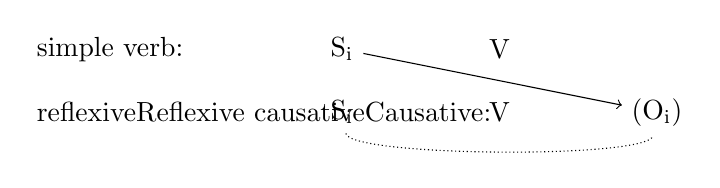
\begin{tikzpicture}[node distance=2cm]

% nodes
\node (x) [anchor=west] at (0, .8) {simple verb:};
\node (x) [anchor=west] at (0, 0) {reflexive\is{Reflexive} causative\is{Causative}:};

\node (S1) at (4, .8) {S\textsubscript{i}};
\node (V1) at (6, .8) {V};
\node (S2) at (4, 0) {S\textsubscript{i}};
\node (V2) at (6, 0) {V};
\node (O) at (8, 0) {(O\textsubscript{i})};

% arrows
\draw [->] (S1) -- (O) ;
\draw[densely dotted] (S2)  to[out=-80,in=-100,distance=.3cm] (O) ;
  

\end{tikzpicture}


}
% \todo[inline]{Add arrow and dotted curve.}

This is illustrated in the following two pairs of examples, first with \textit{riro} ‘become’, then with \textit{takataka} ‘gather’:

\ea\label{ex:8.240}
\gll Ko \textbf{riro} {\ꞌ}ā pē he vārua {\ꞌ}ā. \\
\textsc{prf} become \textsc{cont} like \textsc{pred} spirit \textsc{ident} \\

\glt 
‘He had become like a spirit.’ \textstyleExampleref{[R310.268]} 
\z

\ea\label{ex:8.241}
\gll He uru Taŋaroa ki roto i te vai, he \textbf{haka} \textbf{riro} pa he kahi. \\
\textsc{ntr} enter Tangaroa to inside at \textsc{art} water \textsc{ntr} \textsc{caus} become like \textsc{pred} tuna \\

\glt 
‘Tangaroa entered into the water and turned himself into a tuna.’ \textstyleExampleref{[Fel-046.020]}
\z

\ea\label{ex:8.242}
\gll He oho mai he \textbf{takataka} {\ꞌ}i te hare o te hānautama. \\
\textsc{ntr} go hither \textsc{ntr} gather:\textsc{red} at \textsc{art} house of \textsc{art} pregnant \\

\glt 
‘They came and gathered in the house of the mother-to-be.’ \textstyleExampleref{[Ley-9-55.024]}
\z

\ea\label{ex:8.243}
\gll He \textbf{haka} \textbf{takataka} {\ꞌ}i tū hare era o tū taŋata era. \\
\textsc{ntr} \textsc{caus} gather:\textsc{red} at \textsc{dem} house \textsc{dist} of \textsc{dem} man \textsc{dist} \\

\glt
‘They gathered in the house of that man.’ \textstyleExampleref{[R352.079]} 
\z

These ‘implicit reflexives\is{Reflexive}’ are part of a larger phenomenon: in many cases, causatives do not add a new argument to the verb, so the argument structure of the root is not modified. What addition of \textit{haka} does in such cases, is adding a semantic element, usually an element of agentivity\is{Agentivity}, activity or intensity. For example, while \textit{{\ꞌ}ui} means ‘to ask’, \textit{haka {\ꞌ}ui} is used in the sense ‘to ask persistently and/or repeatedly, to inquire’. Both verbs have the same argument structure, but the causative\is{Causative} verb is more intensive.

\ea\label{ex:8.244}
\gll He \textbf{haka} \textbf{{\ꞌ}ui} mai te aŋa e te ŋā poki repahoa ō{\ꞌ}oku pē nei ē...\\
\textsc{pred} \textsc{caus} ask hither \textsc{art} do \textsc{ag} \textsc{art} \textsc{pl} child friend \textsc{poss.1sg.o} like \textsc{prox} thus\\

\glt
‘My friends kept asking me as follows...’ \textstyleExampleref{[R380.042]} 
\z

\textit{{\ꞌ}Ava{\ꞌ}ava} means ‘to be at a distance’ or ‘to move away, to withdraw’; \textit{haka {\ꞌ}ava{\ꞌ}ava} also has the latter sense, but underlines that the act of withdrawing is volitional. Compare the following pair of examples:

\ea\label{ex:8.245}
\gll Te naonao {\ꞌ}ina he \textbf{{\ꞌ}ava{\ꞌ}ava} rahi mai tō{\ꞌ}ona kona poreko. \\
\textsc{art} mosquito \textsc{neg} \textsc{ntr} distance\_oneself much from \textsc{poss.3sg.o} place born \\

\glt 
‘The mosquito does not go far from its breeding place.’ \textstyleExampleref{[R535.065]} 
\z

\ea\label{ex:8.246}
\gll {\ꞌ}Ina koe ko \textbf{haka} \textbf{{\ꞌ}ava{\ꞌ}ava}. \\
\textsc{neg} \textsc{2sg} \textsc{neg.ipfv} \textsc{caus} distance\_oneself \\

\glt
‘Don’t go away.’ \textstyleExampleref{[R482.045]} 
\z

The same phenomenon can be observed with adjectives. While \textit{haka} + adjective may be a true causative\is{Causative}, expressing that the property is brought about by an external Agent (see (\ref{ex:8.228}–\ref{ex:8.229}) above), it may also express that the subject reaches a state or acquires a property through intentional action. A few examples:

\ea\label{ex:8.246a}
\begin{tabbing}
xxxxxxx \= xxxxxxxxxxxxxxxx \= xxxxxxxxxxxx \= xxxxxxxx \kill
\textit{hāhine} \> ‘to be/draw near’ \> \textit{haka hāhine} \> ‘to approach (volitionally)’\\
\textit{aŋiaŋi} \> ‘to be sure’ \> \textit{haka aŋiaŋi} \> ‘to make sure, verify’\\
\textit{rohirohi} \> ‘to be tired’ \> \textit{haka rohirohi} \> ‘to tire oneself out’
\end{tabbing}
\z

\ea\label{ex:8.247}
\gll He \textbf{haka} \textbf{hāhine} atu o Hotu ki te {\ꞌ}ōpani o tū piha era. \\
\textsc{ntr} \textsc{caus} near away of Hotu to \textsc{art} door of \textsc{dem} room \textsc{dist} \\

\glt 
‘Hotu approached the door of the room.’ \textstyleExampleref{[R301.121]} 
\z

\ea\label{ex:8.248}
\gll Ko haka\_tiu {\ꞌ}ā te repa mai {\ꞌ}uta ki te vaikava  mo \textbf{haka} \textbf{aŋiaŋi} ana ai ko tano {\ꞌ}ā mo hakahonu.\\
\textsc{prf} watch \textsc{cont} \textsc{art} young\_man from inland to \textsc{art} sea  for \textsc{caus} certain:\textsc{red} \textsc{irr} exist \textsc{prf} correct \textsc{cont} for bodysurf\\

\glt 
‘The young men observe the sea to make sure whether the conditions are fit for surfing.’ \textstyleExampleref{[R431.001]} 
\z

\textit{Haka} + adjective or adverb\is{Adverb} may also indicate that the subject acts in a way characterised by the root. As \REF{ex:8.250} shows, this may involve simulating a certain characteristic.\footnote{\label{fn:457}Cf. \citet[14]{Moyle2011} about “similative use” of the causative prefix in \ili{Takuu}.}

\ea\label{ex:8.249}
\gll E \textbf{haka} \textbf{koro{\ꞌ}iti} koe ana vānaŋa mai. \\
\textsc{exh} \textsc{caus} softly \textsc{2sg} \textsc{irr} speak hither \\

\glt 
‘Speak softly (lit. make softly when you speak)!’ \textstyleExampleref{[R408.046]} 
\z

\ea\label{ex:8.250}
\gll Te tire e haŋa rō {\ꞌ}ā mo \textbf{haka} \textbf{{\ꞌ}ata} \textbf{māramarama} i a rāua. \\
\textsc{art} Chile \textsc{ipfv} want \textsc{emph} \textsc{ident} for \textsc{caus} more intelligent \textsc{acc} \textsc{prop} \textsc{3pl} \\

\glt 
‘The Chileans want to pass themselves off as smarter.’ \textstyleExampleref{[R428.006]} 
\z

\subsection{Lexicalised causatives}\label{sec:8.12.5}

A number of \textit{haka} forms have a meaning which cannot quite be predicted from the meaning of the root. Some examples:

\ea
\begin{tabbing}
xxxxxxxxx \= xxxxxxxxxxxxx \= xxxxxxxxxxxxx \= xxxxxxxx \kill
\textit{pāpa{\ꞌ}i} \>  ‘to~write’ \>  \textit{haka~pāpa{\ꞌ}i} \>  ‘to~enrol’\\
\textit{{\ꞌ}omo{\ꞌ}omo} \>  ‘to~suck’ \>  \textit{haka~{\ꞌ}omo{\ꞌ}omo} \>  ‘to~breastfeed’\\
\textit{rivariva} \>  ‘good’ \>  \textit{haka~rivariva} \>  ‘to~improve;~to~prepare’\\
\textit{roŋo} \>  ‘message’ \>  \textit{hakaroŋo} \>  ‘to~listen;~to~perceive’
\end{tabbing}
\z

Another example is found in \REF{ex:8.248} above: \textit{haka honu} ‘bodysurfing’ is a lexicalised causative\is{Causative} from \textit{honu} ‘turtle’. The same sentence also contains the verb \textit{hakatiu} ‘to watch’; even though this is formally a causative, there is no word \textit{tiu} in the Rapa Nui lexicon. There are a few more \textit{haka} forms for which the root as such is not a Rapa Nui word. This includes two very common words: \textit{\mbox{haka{\ꞌ}ou}} ‘again’, \textit{hakarē} ‘to leave (abandon; permit)’. 

\subsection{The causative prefix with nouns}\label{sec:8.12.6}

When the root of the \textit{haka} construction is a noun, the causative\is{Causative} expresses an action which is in some way characterised by the noun. The noun may be the product of the action: \textit{haka N} = ‘to cause the object to be N, to make something into N’, or more generally ‘to make/create N’:

\ea\label{ex:8.251}
\gll He tītiŋi i te ivi ra{\ꞌ}e, he \textbf{haka} \textbf{parehe}.\\
\textsc{ntr} \textsc{pl}:crush \textsc{acc} \textsc{art} bone first \textsc{ntr} \textsc{caus} piece\\

\glt 
‘He crushed the first bone into pieces.’ \textstyleExampleref{[Mtx-3-01.199]}
\z

\ea\label{ex:8.252}
\gll {\ꞌ}I te mahana maha i \textbf{haka} \textbf{kāuŋa} tahi era te ŋā poki. \\
at \textsc{art} day four \textsc{pfv} \textsc{caus} line all \textsc{dist} \textsc{art} \textsc{pl} child \\

\glt
‘On Thursday all the children lined up (formed a line).’ \textstyleExampleref{[R334.139]} 
\z

Other relationships to the noun are possible, whether conventional or creative. In \REF{ex:8.253} the noun refers to something used in the action, or something characterising the direct object as a result of the action. In \REF{ex:8.254} the noun is used in a figurative way (cf. \ili{English} ‘cheeky’). 

\ea\label{ex:8.253}
\gll E \textbf{haka} \textbf{tiare} rō {\ꞌ}ana i a rāua. \\
\textsc{ipfv} \textsc{caus} flower \textsc{emph} \textsc{cont} \textsc{acc} \textsc{prop} \textsc{3pl} \\

\glt 
‘They have adorned themselves with flowers.’ \textstyleExampleref{[R416.415]} 
\z

\ea\label{ex:8.254}
\gll {\ꞌ}Ina ho{\ꞌ}i koe ko \textbf{haka} \textbf{{\ꞌ}āriŋa} ki tu{\ꞌ}u māmā ena.\\
\textsc{neg} indeed \textsc{2sg} \textsc{neg.ipfv} \textsc{caus} face to \textsc{poss.2sg.o} mother \textsc{med}\\

\glt 
‘Don’t be insolent to your mother.’ \textstyleExampleref{[R103.065]} 
\z

\subsection{Lexical causatives}\label{sec:8.12.7}

The term \textit{lexical causative}\is{Causative} refers to a situation where there are two lexemes, unrelated in form, one of which is semantically the causative\is{Causative} of the other. (\citealt[248]{Dixon2012}.) 

There are very few lexical causatives in Rapa Nui; the following two are possible candidates.

\subparagraph{\ref{sec:8.12.7}.1} \textit{Hāŋai} ‘to feed’ can be considered a causative\is{Causative} of \textit{kai} ‘to eat’. Apart from the obvious semantic relationship between the two, there are two reasons to assume a causative\is{Causative} relationship between the two:

%\setcounter{listWWviiiNumvileveli}{0}
\begin{enumerate}
\item 
The morphological causative\is{Causative} \textit{haka kai} does not occur; whenever a causative\is{Causative} of \textit{kai} is called for, \textit{hāŋai} is used. 

\item 
The arguments of \textit{hāŋai} show the same patterns of case-marking as morphological causatives. When the object of eating (the food) is not expressed or implied, the causee (the eater) is expressed as direct object:

\end{enumerate}

\ea\label{ex:8.255}
\gll I tu{\ꞌ}u era he hāŋai \textbf{i} \textbf{a} \textbf{Ure} ka oti rō. \\
\textsc{pfv} arrive \textsc{dist} \textsc{ntr} feed \textsc{acc} \textsc{prop} Ure \textsc{cntg} finish \textsc{emph} \\

\glt
‘When she arrived, she fed Ure completely.’ \textstyleExampleref{[R310.291]} 
\z

But when the object of eating is implied, the causee is marked with \textit{ki}.\footnote{\label{fn:458}There are no examples in the corpus where the causee and the object of eating are both expressed.}

\ea\label{ex:8.256}
\gll He to{\ꞌ}o mai tū kai era, he hāŋai \textbf{ki} \textbf{tū} \textbf{ŋā} \textbf{matu{\ꞌ}a} era o Tiare. \\
\textsc{ntr} take hither \textsc{dem} food \textsc{dist} \textsc{ntr} feed to \textsc{dem} \textsc{pl} parent \textsc{dist} of Tiare \\

\glt
‘They took the food and fed (it) to Tiare’s parents.’ \textstyleExampleref{[R238.009]} 
\z

Not all instances of \textit{hāŋai} can be considered as lexical causatives\is{Causative}, though: the verb is also used in the sense ‘to raise/tend (animals); to raise/rear (children)’.

\subparagraph{\ref{sec:8.12.7}.2} Another possible lexical causative\is{Causative} is \textit{tiŋa{\ꞌ}i} (var. \textit{tiaŋi}) ‘to kill’, causative\is{Causative} of \textit{mate} ‘to die’:

\ea\label{ex:8.257}
\gll He tiŋa{\ꞌ}i i te taŋata, i te vi{\ꞌ}e, i te poki.\\
\textsc{ntr} kill \textsc{acc} \textsc{art} man \textsc{acc} \textsc{art} woman \textsc{acc} \textsc{art} child\\

\glt
‘They killed men, women and children.’ \textstyleExampleref{[Mtx-3-01.250]}
\z

Apart from the sense ‘to kill’, \textit{tīŋa{\ꞌ}i} also has a different (though obviously related) sense: ‘to strike, hit’. Note also that the sense ‘to kill’ is also expressed occasionally by the morphological causative\is{Causative} \textit{haka mate}.

\subparagraph{\ref{sec:8.12.7}.3} A number of causative\is{Causative} verbs were borrowed as a whole from \ili{Tahitian}\is{Tahitian influence}. These are clearly recognizable as borrowings\is{Borrowing}, as they start with \textit{ha{\ꞌ}a-}\is{haa- (causative)@ha{\ꞌ}a- (causative)} ({\textless} Tah. \textit{fa{\ꞌ}a}{}-) rather than \textit{haka}. Most of these are isolated lexical items, the root of which does not occur on its own in Rapa Nui: \textit{ha{\ꞌ}atura} ‘to obey, respect’ (Tah. \textit{tura} ‘respect.N’); \textit{ha{\ꞌ}ati{\ꞌ}a} ‘to permit’ (Tah. \textit{ti{\ꞌ}a} ‘to stand’). For most of these words, it is not at all obvious that \textit{ha{\ꞌ}a-} has a causative\is{Causative} sense in Rapa Nui.

For a few \textit{ha{\ꞌ}a-} forms, however, the root as such was also borrowed into Rapa Nui: \textit{{\ꞌ}ī} ‘to be full’, \textit{ha{\ꞌ}a{\ꞌ}ī} ‘to fill’. As \textit{ha{\ꞌ}a-} is not a productive prefix in Rapa Nui, \textit{ha{\ꞌ}a{\ꞌ}ī} can be considered as a lexical causative\is{Causative} of \textit{{\ꞌ}ī}, rather than a form derived through prefixation of \textit{ha{\ꞌ}a-}.
\is{Causative|)}

\section{Conclusions}\label{sec:8.13}
\largerpage[2]
This chapter has explored the expression of core constituents of verbal clauses.

Rapa Nui patterns with other Polynesian languages in that the S/A argument is marked with \textit{e} or unmarked, while the O argument is marked with \textit{i} or unmarked. However, the resulting case marking patterns are different from those in other languages. At first sight Rapa Nui may seem to have ergative traits, but a close analysis shows that the language is unambiguously accusative. The case marking patterns which seem to deviate from regular accusativity can be explained by the following features:

\begin{itemize}
\item 
obligatory omission of case markers in certain noun phrases, e.g. those containing a prenominal numeral;

\item 
extensive use of the agentive marker \textit{e}, both in transitive and intransitive clauses;

\item 
omission of the object marker \textit{i} in certain clause types;

\item 
a passive construction which is somewhat inconspicuous because of the absence of passive morphology.

\end{itemize}

Agent marking is determined by an interplay of heterogenous factors: syntactic (preverbal subjects are always unmarked), lexico-semantic (some verbs show a strong preference for \textit{e-}marked Agents) and pragmatic (Agents which start to act, tend to be \textit{e}{}-marked). The same is true for object marking: the object marker is omitted under certain conditions, which may be syntactic (OV clauses), lexico-semantic (with certain verbs) or pragmatic (non-salient objects).

Rapa Nui has a passive construction, in which the Patient is expressed as subject while the Agent is an optional oblique (but without morphological changes in the verb). In fact, passivisation in Rapa Nui is part of a wider phenomenon: several (groups of) verbs exhibit variation in argument assignment. For example, the verb \textit{{\ꞌ}ī} ‘to be full’ has two argument structures, with the Container and the Substance as subject, respectively. Variable argument structure can also be observed with transfer verbs like ‘to feed’ and ‘to throw’: with these verbs, either the Patient or the Goal/Recipient is expressed as direct object; the other argument is expressed as an oblique. When the Patient is oblique, it is marked as an instrument (‘he threw the enemy with a spear’). 

Another argument-related operation is the addition of an external Agent to intransitive verbs; this Agent is marked with the preposition \textit{i}.

Rapa Nui has a number of different comitative constructions (‘A with B’). In most of these, a comitative marker is used, followed by the prominence \textit{ko}; this marker is often a plural pronoun (‘Makemake they \textit{ko} Haua’) or collective marker (‘the people together \textit{ko} the priest’). These comitative markers are used in an inclusory way: their number corresponds the total set of referents of both noun phrases. Similar are constructions with comitative sense – but without a comitative marker – in which the first noun phrase is an inclusory pronoun: ‘we \textit{ko} the child’, meaning ‘the child and~I’.

\largerpage[2]
The final topic of this chapter is causativisation. Causativisation is very common in Rapa Nui; moreover, it is very versatile: 

\begin{itemize}
\item 
it can be applied to any verbal predicate and is occasionally applied to nouns as well; 

\item 
it indicates varying types of causation, both direct (‘he made me do it’) and indirect (‘he let me do it, helped me to do it’);

\item 
while a prototypical causative adds an external Agent to the event, some causatives in Rapa Nui do not change the argument structure of the verb, but add an element of intensity or agentivity.

\end{itemize}
\is{Clause!verbal|)}

\chapter[Nonverbal and copular clauses]{Nonverbal and copular clauses}\label{ch:9}
\is{Clause!nominal|(}\section{Introduction}\label{sec:9.1}

This chapter deals with clauses which do not have a lexical verb as predicate. These clauses contain either no verb, an existential verb, or a copula verb. 

The following types can be distinguished and will be discussed in turn: 

\begin{itemize}
\item 
NP NP clauses, i.e. clauses in which both the subject and the predicate are noun phrases (\sectref{sec:9.2});

\item 
existential clauses\is{Clause!existential}, both verbal and non-verbal (\sectref{sec:9.3});

\item 
clauses with a prepositional predicate (\sectref{sec:9.4});

\item 
numerical clauses (\sectref{sec:9.5});

\item 
clauses containing a copula verb (\sectref{sec:9.6}).

\end{itemize}
\section{NP NP clauses}\label{sec:9.2}

When a nominal clause\is{Clause!nominal} consists of two noun phrases, one of them is the subject; for the other noun phrase, there are two possibilities: it may either be referential\is{Referentiality} or non-referential. When the noun phrase is non-referential, it is a true predicate, which gives new information about the subject, expressing that the subject belongs to a certain class. When the non-subject noun phrase is a referential noun phrase, the clause establishes a relation of identity between the two noun phrases, expressing that both are descriptions of the same referent. In this grammar, these two constructions are labelled \textsc{classifying} and \textsc{identifying} clauses\is{Clause!identifying}, respectively.\footnote{\label{fn:459}Various terms are used in the literature. \citet[233]{Dryer2007Clause} distinguishes between “equational clauses” and “true nominal predicate clauses”. The distinction is fundamental in some Polynesian languages; terms used in Pol\is{Clause!equative, equational}ynesian linguistics include: classifying and equative predicates \citep[78]{Bauer1993}, predicational and identificational NPs (\citealt[430]{ChungMason1995}), predicate nominals and equatives (\citealt{DeLacy1999}), class-inclusion and equational sentences \citep[45]{Cook1999}.}

In Rapa Nui, these two types of clauses are distinguished by the use of the predicate marker \textit{he} in classifying clauses\is{Clause!classifying} and the preposition \textit{ko} in identifying clauses\is{Clause!identifying}.

A third type of NP NP clauses, attributive clauses\is{Clause!attributive}, is characterised by the absence of any prenominal marker and the presence of an adjective in the predicate NP.

\subsection{Classifying clauses}\label{sec:9.2.1}
\is{Clause!classifying|(}
In classifying clauses\is{Clause!classifying}, a nominal predicate provides information about the subject by expressing that the subject belongs to a certain class of entities. The predicate is introduced with \textit{he}\is{he (nominal predicate marker)}, which indicates non-referentiality\is{Referentiality} (\sectref{sec:5.3.4}).

The unmarked order\is{Constituent order} in these clauses is Subject–Predicate.

\ea\label{ex:9.1}
\gll A Thor Heyerdahl he científico e tahi.\\
\textsc{prop} Thor Heyerdahl \textsc{ntr} scientist \textsc{num} one\\

\glt 
‘Thor Heyerdahl was a scientist.’ \textstyleExampleref{[R376.007]} 
\z

\ea\label{ex:9.2}
\gll Te toromiro he tumu hauha{\ꞌ}a e tahi. \\
\textsc{art} toromiro \textsc{pred} tree importan \textsc{num} one \\

\glt 
‘The toromiro is an important tree.’ \textstyleExampleref{[R478.053]} 
\z

\ea\label{ex:9.3}
\gll Rā me{\ꞌ}e era pē he tiare he mōrī. \\
\textsc{dist} thing \textsc{dist} like \textsc{pred} flower \textsc{pred} light \\

\glt
‘Those things (that look) like flowers are lights.’ \textstyleExampleref{[R210.199]} 
\z

\is{Constituent order}The predicate may also come first. This happens only when the subject is well-es\-tab\-lished, i.e. topical\is{Topic, topicality} in discourse; it tends to be expressed by a pronoun as in \REF{ex:9.4}, or a generic noun phrase as in \REF{ex:9.5}. In this construction, the predicate is prominent. In \REF{ex:9.5}, for example, the predicate conveys unexpected, surprising information.

\ea\label{ex:9.4}
\gll E ai rō {\ꞌ}ā e tahi taŋata tire, \textbf{he} \textbf{piroto} \textbf{{\ꞌ}avione} a ia. \\
\textsc{ipfv} exist \textsc{emph} \textsc{ident} \textsc{num} one person Chile \textsc{pred} pilot airplane \textsc{prop} \textsc{3sg} \\

\glt 
‘There was one Chilean, he was an airplane pilot.’ \textstyleExampleref{[R378.013]} 
\z

\ea\label{ex:9.5}
\gll \textbf{He} \textbf{taŋata} tau manu era, \textbf{he} \textbf{poki} \textbf{{\ꞌ}a} \textbf{Uho} tau manu era. \\
\textsc{pred} person \textsc{dem} bird \textsc{dist} \textsc{pred} child of\textsc{.a} Uho \textsc{dem} bird \textsc{dist} \\

\glt
‘That bird was a human being, that bird was Uho’s child.’ \textstyleExampleref{[Mtx-7-12.069]}
\z

In \REF{ex:9.6}, Tangaroa (who has transformed himself into a seal, and is mistaken for a seal by the people) wants to emphasise that he is the king, not a real seal as the people think. The predicate \textit{he {\ꞌ}ariki} is counterexpectative and occurs before the subject.\footnote{\label{fn:460}Notice that \textit{ko Taŋaroa}, which is an apposition\is{Apposition} to the predicate, is not fronted but remains in its post-subject position; see sec. \sectref{sec:9.2.5} for more examples of split predicates.} 

\ea\label{ex:9.6}
\gll He raŋi mai te re{\ꞌ}o o te pakia: ‘\textbf{He} \textbf{{\ꞌ}ariki} au ko Taŋaroa’. \\
\textsc{ntr} call hither \textsc{art} voice of \textsc{art} seal \textsc{pred} king \textsc{1sg} \textsc{prom} Tangaroa \\

\glt 
‘The voice of the seal cried: I am king Tangaroa.’ \textstyleExampleref{[Mtx-1-05.008]}
\z

Just as in verbal clauses, the subject of classifying clauses\is{Clause!classifying} may be left out:

\ea\label{ex:9.7}
\gll He aŋi mau {\ꞌ}ā pē nei ē: \textbf{he} \textbf{{\ꞌ}ariki}. \\
\textsc{ntr} true really \textsc{ident} like \textsc{prox} thus \textsc{pred} king \\

\glt 
‘It is true: he is a king.’ \textstyleExampleref{[Fel-46.053]}
\z

\ea\label{ex:9.8}
\gll \textbf{Ta{\ꞌ}e} \textbf{he} \textbf{taŋata}, \textbf{he} \textbf{{\ꞌ}aku{\ꞌ}aku}, pē ira {\ꞌ}ā au. \\
\textsc{conneg} \textsc{pred} person \textsc{pred} spirit like \textsc{ana} \textsc{ident} \textsc{1sg} \\

\glt 
‘That is not a man, it is a spirit, and so am I.’ \textstyleExampleref{[Mtx-7-04.058]}
\z
\is{Clause!classifying|)}

\subsection{Identifying clauses}\label{sec:9.2.2}
\is{ko (prominence marker)!in identifying clauses|(}\is{Clause!identifying|(}
Identifying clauses serve to identify the referent of one noun phrase with the referent of the other noun phrase in the clause. Both NPs are preceded by a \textit{t}{}-determiner (\sectref{sec:5.3.2}) such as the article \textit{te}, indicating that they are referential. In all identifying clauses, one noun phrase is preceded by the prominence marker \textit{ko} (\sectref{sec:4.7.11}). 

A few examples:

\ea\label{ex:9.9}
\gll Te me{\ꞌ}e ena o te pā{\ꞌ}eŋa {\ꞌ}uta ko tō{\ꞌ}oku māmā era. \\
\textsc{art} thing \textsc{med} of \textsc{art} side inland \textsc{prom} \textsc{poss.1sg.o} mother \textsc{dist} \\

\glt 
‘That (person) on the inland side is my mother.’ \textstyleExampleref{[R411.057]} 
\z

\ea\label{ex:9.10}
\gll Pero ko au te suerekao o te hora nei. \\
but \textsc{prom} \textsc{1sg} \textsc{art} governor of \textsc{art} time \textsc{prox} \\

\glt 
‘But I am the governor now (or: the governor now is me).’ \textstyleExampleref{[R201.007]} 
\z

\ea\label{ex:9.11}
\gll Te ŋāŋata mātāmu{\ꞌ}a o Rapa Nui ko te {\ꞌ}ariki era ko Hotu Matu{\ꞌ}a  ananake ko tō{\ꞌ}ona hua{\ꞌ}ai.\\
\textsc{art} men first of Rapa Nui \textsc{prom} \textsc{art} king \textsc{dist} \textsc{prom} Hotu Matu’a  together \textsc{prom} \textsc{poss.3sg.o} family\\

\glt
‘The first people of Rapa Nui were king Hotu Matu’a with his family.’ \textstyleExampleref{[R350.015]} 
\z

Notice that the \textit{ko}{}-marked NP, in the case of a common noun\is{Noun!common}, is always followed by a postnominal demonstrative\is{Demonstrative!postnominal} \textit{nei}, \textit{ena} or \textit{era}; the combination of the article \textit{te} with one of these demonstratives\is{Demonstrative} indicates definiteness\is{Definiteness} (\sectref{sec:4.6.3.1}).

As both noun phrases are referential\is{Referentiality} and definite\is{Definiteness}, and both refer to the same entity, it is not always clear which NP is subject and which is predicate. Constituent order\is{Constituent order} cannot be used as the sole criterion, as both subject and predicate of a nominal clause\is{Clause!nominal} may come first.\footnote{\label{fn:461}See examples (\ref{ex:9.1}–\ref{ex:9.6}) in classifying clauses\is{Clause!classifying}; the same is true in other types of nominal clauses\is{Clause!nominal}, e.g. locative clauses (\sectref{sec:9.4.1}).} It is even questionable whether the term \textit{predicate} is appropriate at all in identifying clauses\is{Clause!identifying} (see \citealt[440]{Anderson2004}): as both noun phrases are referential expressions, they are fundamentally different from predicates, which designate properties or events rather than referring to entities. 

Even so, the terms \textit{subject} and \textit{predicate} may be used in identifying clauses\is{Clause!identifying} in a loose way, in the sense that the subject is the entity to be identified, and the predicate is the identifying expression. In some cases it is clear which NP is the subject, as this NP functions as discourse topic\is{Topic, topicality}. In other cases, however, it is difficult to identify subject and predicate – unless we adopt a simple syntactic definition. As indicated above, in every identifying clause one noun phrase is marked with \textit{ko}, while the other is an unmarked NP. Taking the \textit{ko}{}-marked NP as predicate provides a simple criterion. Moreover, this analysis coincides with the intuitive assignment of subject and predicate in those cases where the distinction is clear: in examples like \REF{ex:9.11}, it is clear that the unmarked NP is subject, while the \textit{ko}-marked NP serves to identify this subject.

In the examples so far, the identifying clause consists of two common noun phrases. When the clause contains a pronoun or proper noun, the use of \textit{ko} is described by the following two rules:

%\setcounter{listWWviiiNumcileveli}{0}
\begin{enumerate}
\item 
If the clause contains a proper noun\is{Noun!proper}, this is always \textit{ko}{}-marked.

\item 
If the clause contains a pronoun\is{Pronoun!personal}, this is usually \textit{ko}{}-marked,\footnote{\label{fn:462}I have not found any exceptions to this rule in the text corpus, though there are a few exceptions in the New Testament translation.} unless the other constituent is a proper noun.

\end{enumerate}

This is illustrated in the following examples.

Common NP\is{Noun!common} + proper noun:

\ea\label{ex:9.12}
\gll Te kona hope{\ꞌ}a o te nehenehe \textbf{ko} \textbf{{\ꞌ}Anakena}. \\
\textsc{art} place last of \textsc{art} beautiful \textsc{prom} Anakena \\

\glt
‘The most beautiful place (of the island) is Anakena.’ \textstyleExampleref{[R350.013]} 
\z

Pronoun + common NP:

\ea\label{ex:9.13}
\gll Pero \textbf{ko} \textbf{au} te suerekao o te hora nei. \\
but \textsc{prom} \textsc{1sg} \textsc{art} governor of \textsc{art} time \textsc{prox} \\

\glt
‘But I am the governor now (or: the governor now is me).’ \textstyleExampleref{[R201.007]} 
\z

Pronoun + proper noun:

\ea\label{ex:9.14}
\gll A au \textbf{ko} \textbf{Omoaŋa}. \\
\textsc{prop} \textsc{1sg} \textsc{prom} Omoanga \\

\glt
‘I am Omoanga.’ \textstyleExampleref{[R314.101]} 
\z

These patterns make sense if we assume that \textit{ko} always marks the predicate. Proper names are inherently highly identifiable\is{Identifiability} (their reference is always unique and unambiguous in a given context), so it is not surprising that they serve as an identifying expression (predicate) rather than as a referent to be identified (subject). The same is true for pronouns. Between proper nouns\is{Noun!proper} and pronouns, the former are identifiable to a higher degree\is{Identifiability}: within a given context, a proper noun has unambiguous unique reference; for a pronoun, more contextual clues may be needed to establish its reference. This can be represented in a \textit{hierarchy of identifiability}\is{Identifiability}:

\ea\label{ex:9.14a}
  proper nouns\is{Noun!proper} {\textgreater} pronouns {\textgreater} common nouns\is{Noun!common}
\z

The idea that \textit{ko} marks the predicate is also confirmed by the fact that an identifying clause may consist of a \textit{ko}-phrase only; this follows from the general rule in Rapa Nui that the predicate is obligatory, while the subject can be omitted:

\ea\label{ex:9.15}
\gll —¿Ko ai koe? —\textbf{Ko} \textbf{au} \textbf{{\ꞌ}ana}. \\
~~~~~\textsc{prom} who \textsc{2sg} ~~~\textsc{prom} \textsc{1sg} \textsc{ident} \\

\glt 
‘—Who are you? —It’s me.’ \textstyleExampleref{[Mtx-7-04.071–072]}
\z

\ea\label{ex:9.16}
\gll —Me{\ꞌ}e era ko Tito. —{\ꞌ}Ēē. \textbf{Ko} \textbf{ia}. \\
~~~thing~ \textsc{dist} \textsc{prom} Tito ~~~yes \textsc{prom} \textsc{3sg} \\

\glt 
‘—That one (in the picture) is Tito. —Yes. It’s him.’ \textstyleExampleref{[R414.163–165]}
\z

In \REF{ex:9.14} above, the pronoun is not marked with \textit{ko} when the other constituent is a proper noun. There are also a few cases in the corpus where a pronoun and a proper noun are both \textit{ko}{}-marked. Two examples are provided below:

\ea\label{ex:9.17}
\gll Ko au ko Totimo. \\
\textsc{prom} \textsc{1sg} \textsc{prom} Totimo \\

\glt 
‘I am Totimo.’ \textstyleExampleref{[R399.193]} 
\z

\ea\label{ex:9.18}
\gll —¿Ko ai koe? —Ko au ko Huri {\ꞌ}Avai. \\
~~~~~\textsc{prom} who \textsc{2sg} ~~~\textsc{prom} \textsc{1sg} \textsc{prom} Huri Avai \\

\glt
‘—Who are you? —I am Huri Avai.’ \textstyleExampleref{[Mtx-3-01.127–128]}
\z

If the pronoun is taken as the subject, these clauses are counterexamples to the claim that only the predicate is marked with \textit{ko}. However, a different analysis is also possible: the pronoun can be analysed as the predicate (with implicit subject), with the proper noun added as apposition\is{Apposition}, ‘It’s me, Totimo’. In both examples above this analysis is plausible. In \REF{ex:9.17}, for example, the situation is as follows: there is a blind girl, Mahina Tea, who knows a boy called Totimo. Totimo walks up to her, embraces her and utters the clause quoted here. An analysis as predicate + apposition\is{Apposition} is appropriate here.\footnote{\label{fn:463}This analysis is reinforced by the fact that in some cases the two constituents are separated by a comma:
\ea \gll 
Ko au, ko Hotu {\ꞌ}Iti te Mata{\ꞌ}iti {\ꞌ}a Hotu Matu{\ꞌ}a.\\
  \textsc{prom} \textsc{1sg} \textsc{prom} Hotu Iti te Mata’iti of\textsc{.a} Hotu Matu’a\\
  \glt 
  ‘It’s me, Hotu Iti te Mata’iti, son of Hotu Matu’a.’ (Ley-2-08.025)\z } 

In other cases this analysis is less plausible, as in the following exchange:

\ea\label{ex:9.19}
\gll —¿Ko ai koe? ... —¡\textbf{Ko} \textbf{au} nei \textbf{ko} \textbf{Vaha} ko to{\ꞌ}o i a Huri {\ꞌ}a Vai! ... —¡{\ꞌ}E \textbf{ko} \textbf{au} nei \textbf{ko} \textbf{Kaiŋa} ko to{\ꞌ}o i a Vaha! \\
~~~~~\textsc{prom} who \textsc{2sg}  ~ ~~~\textsc{prom} \textsc{1sg} \textsc{prox} \textsc{prom} Vaha \textsc{prom} take \textsc{acc} \textsc{prop} huri a Vai  ~ ~~~~and \textsc{prom} \textsc{1sg} \textsc{prox} \textsc{prom} Kainga \textsc{prom} take \textsc{acc} \textsc{prop} Vaha \\

\glt
‘—Who are you? —I am Vaha, who takes (=kills) Huri a Vai! —And I am Kainga, who takes Vaha!’ \textstyleExampleref{[R304.97-101]}
\z

Especially in the last clause, an appositional analysis doesn’t appear to be appropriate. Possibly, these constructions can be analysed as topic + comment constructions (\sectref{sec:8.6.1.3}): ‘(As for) me, I’m Kainga.’\footnote{\label{fn:464}\citet[47]{DeLacy1999} discusses cases in \ili{Māori} where both constituents are \textit{ko}-marked; these are different in that both constituents are a (long) common noun phrase. This enables De Lacy to analyse these as clefts, i.e. biclausal constructions.} 

\subsection{Comparing classifying and identifying clauses}\label{sec:9.2.3}

In the examples of classifying clauses in \sectref{sec:9.2.1} above, the predicate NP clearly indicates that the subject belongs to a certain class of entities; the subject is part of a category described by the predicate. 

In some cases however, the class of entities described by the predicate has only one member, i.e. this class coincides with the referent of the subject. This is illustrated in the following examples:

\ea\label{ex:9.20}
\gll A Tiki \textbf{he} \textbf{poki} o te ra{\ꞌ}ā {\ꞌ}e \textbf{he} \textbf{{\ꞌ}atua} \textbf{rahi} o rāua. \\
\textsc{prop} Tiki \textsc{pred} child of \textsc{art} sun and \textsc{pred} god great of \textsc{3pl} \\

\glt 
‘Tiki was the son of the sun and their high God.’ \textstyleExampleref{[R376.027]} 
\z

\ea\label{ex:9.21}
\gll A au \textbf{he} \textbf{pū{\ꞌ}oko} \textbf{o} \textbf{Rapa} \textbf{Nui} {\ꞌ}i te ao ta{\ꞌ}ato{\ꞌ}a. \\
\textsc{prop} \textsc{1sg} \textsc{pred} head of Rapa Nui at \textsc{art} world all \\

\glt 
‘I am the head (leader) of Rapa Nui in the whole world.’ \textstyleExampleref{[R648.290]} 
\z

\ea\label{ex:9.22}
\gll A ia \textbf{he} \textbf{matu{\ꞌ}a} \textbf{tane} o tō{\ꞌ}oku matu{\ꞌ}a vahine. \\
\textsc{prop} \textsc{3sg} \textsc{pred} parent male of \textsc{poss.1sg.o} parent female \\

\glt
‘He is the father of my mother.’ \textstyleExampleref{[R487.040]} 
\z

These clauses are very similar in sense to identifying clauses\is{Clause!identifying}, which express that two noun phrases have identical reference (\sectref{sec:9.2.2}). In fact, in most examples above, the predicate is translated with a definite noun phrase in \ili{English}, which is characteristic of an identifying clause. Some examples of identifying clauses\is{Clause!identifying} are very similar to the classifying clauses above:

\ea\label{ex:9.23}
\gll He {\ꞌ}ite ia Tu{\ꞌ}u Koihu {\ꞌ}i tū hora era tū ŋā nu{\ꞌ}u era  \textbf{ko} \textbf{tū} \textbf{ŋā} \textbf{tahutahu} \textbf{era}.\\
\textsc{ntr} know then Tu’u Koihu at \textsc{dem} time \textsc{dist} \textsc{dem} \textsc{pl} people \textsc{dist}  \textsc{prom} \textsc{dem} \textsc{pl} witch \textsc{dist}\\

\glt 
‘At that moment Tu’u Koihu knew that those people (whom he saw) were those witches.’ \textstyleExampleref{[R233.023]} 
\z

\ea\label{ex:9.24}
\gll Te hau era, ho{\ꞌ}i, e hī era \textbf{ko} \textbf{te} \textbf{ŋā} \textbf{hau} \textbf{hiro} \textbf{era} e toru kave. \\
\textsc{art} cord \textsc{dist} indeed \textsc{ipfv} to\_fish \textsc{dist} \textsc{prom} \textsc{art} \textsc{pl} cord braid \textsc{dist} \textsc{num} three fibre \\

\glt
‘(in a description of fishing techniques:) The lines they fished with, were those lines braided with three strands.’ \textstyleExampleref{[R539-1.218]}
\z

These examples show that the choice between the two constructions in Rapa Nui is not determined by the criterion of uniqueness, that is, whether or not the predicate defines a single unique entity.\footnote{\label{fn:465}\citet{Lyons1999} mentions uniqueness as one of the necessary conditions for definiteness\is{Definiteness}. Uniqueness is defined as: “there is only one entity satisfying the description used, relative to the context.”} Rather, classifying constructions serve to \textit{describe} the subject by giving new information about it, while identifying clauses\is{Clause!identifying} serve to \textit{identify} a referent with an entity already known to the hearer. The referent of the identifying noun phrase must be accessible\is{Accessibility} to the hearer, otherwise a classifying construction with \textit{he} is used.

To give an example, in the context preceding \REF{ex:9.20} above, there has been no mention of the son of the sun and the high God, so the hearer does not necessarily know that there is such a person as the child of the sun, or that the people in the story had a high God at all. Therefore, this person is not accessible to the hearer. By contrast, in \REF{ex:9.23}, ‘those witches’ refers to witches who have been mentioned earlier in the story; the identifying clause enables the hearer to identify this known entity with the subject ‘those people’. Similarly, in \REF{ex:9.24} the speaker refers to a type of fishing line which he assumes to be known by the hearer (even though it has not been mentioned in the text itself).

The referent of a noun phrase in an identifying clause must not only be unique and accessible\is{Accessibility}, it also needs to be a specific\is{Specific reference}, bounded entity. In the following two examples, the predicate noun phrase could be considered as unique and accessible; nevertheless, it is marked with \textit{he}\is{he (nominal predicate marker)}, i.e. the construction is a classifying clause\is{Clause!classifying}. In \REF{ex:9.25}, the noun phrase refers to priests in general, not to any specific priest. Likewise, in \REF{ex:9.26}, the reference is to adults in general.\footnote{\label{fn:466}These examples are cleft\is{Cleft} constructions, which are discussed in more detail in sec. \sectref{sec:9.2.6} below.}

\ea\label{ex:9.25}
\gll \textbf{He} \textbf{ivi{\ꞌ}atua} \textbf{nō} te kope era e puā era {\ꞌ}i te ta{\ꞌ}u era i a ia te {\ꞌ}ao. \\
\textsc{pred} priest just \textsc{art} person \textsc{dist} \textsc{ipfv} touch \textsc{dist} at \textsc{art} year \textsc{dist} at \textsc{prop} \textsc{3sg} \textsc{art} reign \\

\glt 
‘The priest was the only person (lit. only the priest was the person) who would touch him (te bird man) in the year in which he reigned.’ \textstyleExampleref{[R641.008]} 
\z

\ea\label{ex:9.26}
\gll Te ŋā poki ko {\ꞌ}ite {\ꞌ}ana o ruŋa i te me{\ꞌ}e ta{\ꞌ}ato{\ꞌ}a o te naonao {\ꞌ}e \textbf{he} \textbf{pa{\ꞌ}ari} te me{\ꞌ}e i ta{\ꞌ}e {\ꞌ}ite. \\
\textsc{art} \textsc{pl} child \textsc{prf} know \textsc{cont} of above at \textsc{art} thing all of \textsc{art} mosquito and \textsc{pred} adult \textsc{art} thing \textsc{pfv} \textsc{conneg} know \\

\glt 
‘The children know everything about the mosquitoes, and the adults are the ones who don’t know.’ \textstyleExampleref{[R535.159]} 
\z

We may conclude that a nominal predicate designating an accessible\is{Accessibility}, individuated, bounded entity is marked with \textit{ko}; in all other cases, a classifying construction with \textit{he}\is{he (nominal predicate marker)} is used. A similar difference between \textit{ko} and \textit{he} can be observed with topicalisation in verbal clauses (\sectref{sec:8.6.2}).

As the examples above show, classifying predicates always consist of a common noun phrase. Proper nouns\is{Noun!proper} and pronouns never serve as a classifying predicate; in fact, they are never preceded by \textit{he}. This is to be expected, as proper nouns\is{Noun!proper} and pronouns by definition qualify as identifying predicates: they have unique reference, are accessible in the context, and refer to a specific, bounded entity. On the other hand, they do not designate a class of entities, hence are not suitable as classifying predicates.

\subsection{Constituent order in identifying clauses}\label{sec:9.2.4}
\is{Constituent order}\is{Clause!identifying}
The order of constituents in an identifying clause depends to some extent on the type of noun phrases involved. When both constituents are common noun phrases, the predicate usually occurs after the subject, as illustrated in (\ref{ex:9.23}–\ref{ex:9.24}) and \REF{ex:9.11} above. The predicate may come first when it conveys significant and possibly surprising information as in \REF{ex:9.27}, or when it is a discourse topic established in the preceding context as in \REF{ex:9.28}.\footnote{\label{fn:467}Cf. \citet{Levinsohn2007}: prominence may involve both new information (focal prominence) and established information (thematic\is{Thematicity} prominence).}

\ea\label{ex:9.27}
\gll Ta{\ꞌ}e he {\ꞌ}atua tau me{\ꞌ}e era, he taŋata; \textbf{ko} \textbf{te} \textbf{ŋā} \textbf{io} \textbf{era} \textbf{{\ꞌ}Āmai} tau me{\ꞌ}e era.\\
\textsc{conneg} \textsc{pred} god \textsc{dem} thing \textsc{dist} \textsc{pred} person \textsc{prom} \textsc{art} \textsc{pl} youngster \textsc{dist} Amai \textsc{dem} thing \textsc{dist}\\

\glt 
‘These beings are not gods, they are men; these beings are the Amai guys.’ \textstyleExampleref{[Mtx-7-37.029]}
\z

\ea\label{ex:9.28}
\gll \textbf{Ko} \textbf{te} \textbf{me{\ꞌ}e} \textbf{nei} te me{\ꞌ}e u{\ꞌ}i rahi o te mu{\ꞌ}a {\ꞌ}ā. \\
\textsc{prom} \textsc{art} thing \textsc{prox} \textsc{art} thing see much of \textsc{art} front \textsc{ident} \\

\glt
‘This (= the difficulties mentioned in the previous clause) was something often seen in the past.’ \textstyleExampleref{[R107.009]} 
\z

When the identifying clause contains a pronoun (whether subject or predicate), this is always in an initial position, as illustrated in (\ref{ex:9.13}–\ref{ex:9.14}) above. 

When the clause consists of a proper noun and a common noun phrase, they may occur in either order, as the following examples show. Putting the predicate before the subject gives it more prominence\is{Prominence}. In \REF{ex:9.31}, for example, the predicate \textit{ko Korikē} is contrasted with other persons. In \REF{ex:9.32}, Anakena is singled out between other places on the island.

\ea\label{ex:9.29}
\gll Te kona hope{\ꞌ}a o te nehenehe \textbf{ko} \textbf{{\ꞌ}Anakena}. \\
\textsc{art} place last of \textsc{art} beautiful \textsc{prom} Anakena \\

\glt 
‘The most beautiful place is Anakena.’ \textstyleExampleref{[R350.013]} 
\z

\ea\label{ex:9.30}
\gll Te matu{\ꞌ}a o Hotu Matu{\ꞌ}a \textbf{ko} \textbf{Ta{\ꞌ}ane} \textbf{Arai}. \\
\textsc{art} parent of Hotu Matu’a \textsc{prom} Ta’ane Arai \\

\glt 
‘The father of Hotu Matu’a was Ta’ane Arai.’ \textstyleExampleref{[Ley-2-01.003]}
\z

\ea\label{ex:9.31}
\gll ¿\textbf{Ko} \textbf{Korikē} te me{\ꞌ}e nei {\ꞌ}o ko Titata? ... ¿\textbf{Ko} \textbf{Titata} te me{\ꞌ}e nei? \\
~\textsc{prom} Korike \textsc{art} thing \textsc{prox} or \textsc{prom} Titata  ~ ~\textsc{prom} Titata \textsc{art} thing \textsc{prox} \\

\glt 
‘(pointing at someone in a picture:) Is this Korike or Titata? Is it Titata?’ \textstyleExampleref{[R415.568–572]}
\z

\ea\label{ex:9.32}
\gll \textbf{Ko} \textbf{{\ꞌ}Anakena} \textbf{mau} \textbf{nō} te kona kai māuiui {\ꞌ}ā e noho mai ena. \\
\textsc{prom} Anakena really just \textsc{art} place \textsc{neg.pfv} sick \textsc{cont} \textsc{ipfv} stay hither \textsc{med} \\

\glt 
‘Anakena was the only place where the people who lived there did not get sick.’ \textstyleExampleref{[R231.098]}\textstyleExampleref{} 
\z

\subsection{Split predicates}\label{sec:9.2.5}
\is{Constituent order}\is{Split predicate|(}
When a clause has a pronominal subject and the predicate comes first, certain postnominal modifiers of the predicate are placed after the subject. In \REF{ex:9.33}, \textit{\mbox{ō{\ꞌ}ou}} is a postnominal possessive modifying the predicate \textit{repahoa}; it is separated from the nucleus by the subject \textit{au}. 

\ea\label{ex:9.33}
\gll He repahoa nō \textbf{au} ō{\ꞌ}ou. \\
\textsc{pred} friend just \textsc{1sg} \textsc{poss.2sg.o} \\

\glt
‘I am just your friend.’ \textstyleExampleref{[R308.032]} 
\z

This predicate split is obligatory; clauses like the following do not occur:

\ea\label{ex:9.34}
\textit{*He repahoa nō ō{\ꞌ}ou au.}
\z

As discussed in \sectref{sec:4.6.6}, this process also takes place when the subject is a demonstrative pronoun; this is illustrated in (\ref{ex:9.35}–\ref{ex:9.36}) below. The stranded\is{Stranding} element is often a possessive as in \REF{ex:9.33}; it may also be a numeral as in \REF{ex:9.35}, or a relative clause\is{Clause!relative} as in \REF{ex:9.36}. While in \REF{ex:9.36} the relative clause as a whole is separated from the head noun \textit{famiria}, in \REF{ex:9.37} the relative clause itself is split up: the verb phrase\is{Clause!relative} (\textit{aŋa mau {\ꞌ}ā}) moves along with the head noun, while the direct object is stranded after the subject (\sectref{sec:11.4.5} on raising of relative clause\is{Clause!relative} verbs). 

\ea\label{ex:9.35}
\gll He {\ꞌ}a{\ꞌ}amu nō \textbf{nei} e tahi...\\
\textsc{pred} story just \textsc{prox} \textsc{num} one\\

\glt 
‘This (what follows) is a story...’ \textstyleExampleref{[Luke 11:5]}
\z

\ea\label{ex:9.36}
\gll Famiria hope{\ꞌ}a \textbf{rā} oho mai mai kampō, mai {\ꞌ}Anakena. \\
family last \textsc{dist} go hither from countryside from Anakena \\

\glt 
‘This was the last family who came from the countryside, from Anakena.’ \textstyleExampleref{[R413.889]} 
\z

\ea\label{ex:9.37}
\gll He vi{\ꞌ}e {\ob}aŋa mau {\ꞌ}ā\,{\cb} \textbf{a} \textbf{ia} {\ob}i te me{\ꞌ}e haŋa o te {\ꞌ}Atua\,{\cb}. \\
\textsc{pred} woman {\db}do really \textsc{ident} \textsc{prop} \textsc{3sg} {\db}\textsc{acc} \textsc{art} thing want of \textsc{art} God \\

\glt
‘She is a woman who really does the things God wants.’ \textstyleExampleref{[1 Tim. 5:10]}
\z

Split constituents also occur around the particle \textit{ia}\is{ia ‘then’} ‘then’ (\sectref{sec:4.5.4.1}), which occurs after the first constituent of the clause; postnuclear elements occur after \textit{ia}:

\ea\label{ex:9.38}
\gll Te matu{\ꞌ}a vahine \textbf{ia} o Hēmi he ha{\ꞌ}amata he mana{\ꞌ}u.... \\
\textsc{art} parent female then of Hemi \textsc{ntr} begin \textsc{ntr} think \\

\glt 
‘Then Hemi’s mother started to think...’ \textstyleExampleref{[R476.042]} 
\z

\ea\label{ex:9.39}
\gll {\ꞌ}I tu{\ꞌ}a \textbf{ia} o Kālia e tahi io {\ꞌ}ā{\ꞌ}ana i ohu atu...\\
at back then of Kalia \textsc{num} one young\_man \textsc{poss.3sg.a} \textsc{pfv} shout away\\

\glt 
‘Behind Kalia, one young man of her (family) shouted...’ \textstyleExampleref{[R345.084]} 
\z

\citet[119–120]{Clark1976} analyses this process as extraposition of the second constituent of the predicate over the subject. Alternatively, the split can be described as movement of the predicate with stranding\is{Stranding} of the postnominal modifier; fronting of a constituent is a common process (both crosslinguistically and in Rapa Nui), while it is difficult to see why a modifier would be moved to the right.
\is{Split predicate|)}
\subsection{Clefts}\label{sec:9.2.6}
\is{Cleft|(}
A cleft\is{Cleft} construction consists of two noun phrases, one of which is a simple noun phrase, while the other contains a relative clause\is{Clause!relative}, often without head noun \citep[278]{Payne1997}. Clefts are formally identifying clauses\is{Clause!identifying} – their main constituents are two coreferential NPs – but they express an event or action; the latter is relegated to the relative clause\is{Clause!relative}. The effect of a cleft\is{Cleft} construction is to put the simple NP in focus\is{Focus}.

In Rapa Nui cleft\is{Cleft} constructions, the simple NP comes first and is marked with \textit{ko}, as is expected with predicates of identifying clauses (\sectref{sec:9.2.2}). The second noun phrase contains an anchor noun functioning as head of the relative clause\is{Clause!relative}; this is either a repetition of the noun in focus, or a generic noun like \textit{me{\ꞌ}e}\is{mee ‘thing’@me{\ꞌ}e ‘thing’} ‘thing’. The cleft\is{Cleft} construction is thus similar to the \ili{English} construction ‘Mary was the one who won’,\footnote{\label{fn:468}Cleft constructions of the type ‘X was the one who...’ are often called pseudo-clefts (\citealt[279]{Payne1997}; \citealt[9]{Bauer1991} for \ili{Māori}). On the question whether Rapa Nui also has “real” clefts, i.e. without anchor noun, see sec. \sectref{sec:8.6.2.1}.} though a noun is used instead of ‘one’ and there is no copula verb. As in all relative clauses\is{Clause!relative}, the verb is usually marked with \textit{i}, \textit{e} or unmarked (\sectref{sec:11.4.3}).

A few examples:

\ea\label{ex:9.40}
\gll Ko te nūna{\ꞌ}a era {\ꞌ}a {\ꞌ}Ōrare {\ob}te nūna{\ꞌ}a i rē\,{\cb}. \\
\textsc{prom} \textsc{art} group \textsc{dist} of\textsc{.a} Orare {\db}\textsc{art} group \textsc{pfv} win \\

\glt 
‘(in a report about a music contest:) Orare’s group was the group that won.’ \textstyleExampleref{[R539-3.313]}
\z

\ea\label{ex:9.41}
\gll Ko te ŋā me{\ꞌ}e nei {\ob}te me{\ꞌ}e mo ai o te taŋata  mo oho mo ruku o te hora nei\,{\cb}.\\
\textsc{prom} \textsc{art} \textsc{pl} thing \textsc{prox} {\db}\textsc{art} thing for exist of \textsc{art} person  for go for dive of \textsc{art} time \textsc{prox}\\

\glt 
‘These things (which have just been listed) are the things that people need to go diving nowadays.’ \textstyleExampleref{[R360.002]} 
\z

\ea\label{ex:9.42}
\gll Ko mātou nō {\ob}te me{\ꞌ}e noho o nei\,{\cb}. \\
\textsc{prom} \textsc{1pl.excl} only {\db}\textsc{art} thing stay of \textsc{prox} \\

\glt 
‘(in the description of a house:) We are the only ones living here.’ \textstyleExampleref{[R404.050]} 
\z

\ea\label{ex:9.43}
\gll Ko Timo {\ob}te me{\ꞌ}e {\ꞌ}ori tako{\ꞌ}a o roto nei\,{\cb}. \\
\textsc{prom} Timo {\db}\textsc{art} thing dance also of inside \textsc{prox} \\

\glt
‘Timo is the one who is also dancing inside (= in this picture).’ \textstyleExampleref{[R414.129]} 
\z

The effect of relegating the verb to a relative clause\is{Clause!relative} is that the initial noun phrase is in focus\is{Focus}, while the event or action is backgrounded. Clefts are used when the event or action as such is presupposed; it has already been mentioned as in \REF{ex:9.41}, or can be inferred from the context: in \REF{ex:9.40}, the context of a musical contest presupposes that there is a winner, while the important new information is the identity of the winner. The act of winning is therefore backgrounded, while the noun phrase referring to the winner is put in focus.

The examples so far represent the most common construction, in which clefts are constructed as identifying clauses\is{Clause!identifying} with a \textit{ko}{}-marked predicate. Clefts may also be classifying clauses\is{Clause!classifying}, with a \textit{he}{}-marked predicate. As discussed in \sectref{sec:9.2.1}, identifying clauses\is{Clause!identifying} are used when the predicate refers to a unique individual which is accessible to the hearer; in other cases, classifying clauses\is{Clause!classifying} are used. This happens for example when the noun phrase is generic:

\ea\label{ex:9.44}
\gll Te ŋā poki ko {\ꞌ}ite {\ꞌ}ana o ruŋa i te me{\ꞌ}e ta{\ꞌ}ato{\ꞌ}a o te naonao {\ꞌ}e \textbf{he} \textbf{pa{\ꞌ}ari} {\ob}te me{\ꞌ}e i ta{\ꞌ}e {\ꞌ}ite\,{\cb}. \\
\textsc{art} \textsc{pl} child \textsc{prf} know \textsc{cont} of above at \textsc{art} thing all of \textsc{art} mosquito and \textsc{pred} adult {\db}\textsc{art} thing \textsc{pfv} \textsc{conneg} know \\

\glt 
‘The children know everything about the mosquitoes, and the adults are the ones who don’t know.’ \textstyleExampleref{[R535.159]} 
\z

Classifying\is{Clause!classifying} cleft\is{Cleft} constructions are especially common with the verb \textit{haŋa} ‘want’ and other expressions of volition\is{Verb!volition}/desire (\sectref{sec:3.2.3.1.1} on the nominal tendency of volition verbs). With these verbs, the noun phrase does not contain a full relative clause\is{Clause!relative}, but a bare modifying verb, such as \textit{haŋa} in \REF{ex:9.45}; if the subject of this verb is expressed, it is a possessive pronoun (\textit{tā{\ꞌ}aku} in \REF{ex:9.45}) or a genitive phrase (\sectref{sec:11.4.4}):

\ea\label{ex:9.45}
\gll \textbf{He} \textbf{kāpē} tā{\ꞌ}aku me{\ꞌ}e haŋa. \\
\textsc{pred} coffee \textsc{poss.1sg.a} thing want \\

\glt 
‘Coffee is what I want (lit. my thing want).’ \textstyleExampleref{[R221.024]} 
\z

\ea\label{ex:9.46}
\gll Mō{\ꞌ}ona te me{\ꞌ}e manava mate \textbf{he} \textbf{hoi} \textbf{eke}... \\
\textsc{ben.3sg.o} \textsc{art} thing stomach die{\rmfnm} \textsc{pred} horse climb \\

\glt 
‘For him, the thing (he) liked most was climbing his horse (and going around the island).’ \textstyleExampleref{[R439.008]} 
\z
\footnotetext{\textit{Manava mate} is an idiom expressing love or endearment.}

Clefts also occur in questions, when a verb argument is questioned: identifying clefts with \textit{ko ai}\is{ai ‘who’} ‘who’ (\sectref{sec:10.3.2.1}), classifying clefts with \textit{he aha}\is{aha ‘what’} ‘what’ (\sectref{sec:10.3.2.2}).

As discussed in \sectref{sec:8.6.3}, the actor-emphatic\is{Actor-emphatic construction} (AE) construction also serves to put a noun phrase in focus\is{Focus}. It is not entirely clear which conditions determine the choice between an AE construction and a cleft\is{Cleft}. However, AE’s are only used to put agentive subjects in focus; in order to put non-agentive subjects in focus as in \REF{ex:9.41} or non-subjects as in \REF{ex:9.45}, only clefts can be used.
\is{ko (prominence marker)!in identifying clauses|)}\is{Clause!identifying|)}\is{Cleft|)}

\subsection{Attributive clauses}\label{sec:9.2.7}
\is{Clause!attributive|(}
In an attributive clause, an inherent – and usually permanent – property is attributed to the subject.\footnote{\label{fn:470}Non-permanent properties are expressed as verbal predicates, see sec. \sectref{sec:3.5.1.5}.} This property is in most cases expressed as an adjective. Now an adjective as such cannot serve as a nominal predicate in Rapa Nui, and therefore an anchor noun is needed to fit the adjective into the syntactic structure. This anchor noun is either identical to the subject noun or a generic noun like \textit{me{\ꞌ}e}\is{mee ‘thing’@me{\ꞌ}e ‘thing’} ‘thing’.\footnote{\label{fn:471}In related languages, cognates of \textit{me{\ꞌ}e} also serve as anchor noun for adjectival or verbal predicates; see e.g. \citet[38]{LazardPeltzer2000} on \ili{Tahitian}.} 

The predicate may be marked with \textit{he}\is{he (nominal predicate marker)} as in \REF{ex:9.47}, in which case the clause is a classifying clause\is{Clause!classifying} (\sectref{sec:9.2.1}). This is rare, though; usually the predicate is a bare noun phrase, lacking any determiner.

Below are some examples, with the anchor noun emphasised.

With repetition of the subject noun:

\ea\label{ex:9.47}
\gll Te {\ꞌ}ati ena o te kahu {\ꞌ}i rā noho iŋa \textbf{he} \textbf{{\ꞌ}ati} nuinui e tahi. \\
\textsc{art} problem \textsc{med} of \textsc{art} clothes at \textsc{dist} stay \textsc{nmlz} \textsc{pred} problem big:\textsc{red} \textsc{num} one \\

\glt 
‘The problem of clothing at the time was a big one.’ \textstyleExampleref{[R380.093]} 
\z

\ea\label{ex:9.48}
\gll \textbf{Taŋata} {\ꞌ}uri{\ꞌ}uri te taŋata nei {\ꞌ}e \textbf{taŋata} rakerake. \\
person black:\textsc{red} \textsc{art} person \textsc{prox}\textsc{} and person bad:\textsc{red} \\

\glt
‘This man is dark and ugly.’ \textstyleExampleref{[R372.133]} 
\z

With a generic noun:

\ea\label{ex:9.49}
\gll Māuiui nei \textbf{me{\ꞌ}e} rakerake, me{\ꞌ}e pe{\ꞌ}e. \\
sick \textsc{prox} thing bad:\textsc{red} thing infect \\

\glt 
‘This disease was serious, it was contagious.’ \textstyleExampleref{[R231.318]} 
\z

\ea\label{ex:9.50}
\gll \textbf{Me{\ꞌ}e} {\ꞌ}iti{\ꞌ}iti koe {\ꞌ}i roto i te vaikava. \textbf{Me{\ꞌ}e} nuinui koe mō{\ꞌ}oku... \\
thing small:\textsc{red} \textsc{2sg} at inside at \textsc{art} ocean thing big:\textsc{red} \textsc{2sg} \textsc{ben.1sg.o} \\

\glt
‘You are a little thing in the ocean. You are big to me...’ \textstyleExampleref{[R474.007]} 
\z

These examples show that, as in other nominal clauses\is{Clause!nominal}, either the subject may come first as in \REF{ex:9.47} and \REF{ex:9.49}, or the predicate as in \REF{ex:9.48} and \REF{ex:9.50}.

In the examples above, the property is an adjective. It may also be another type of noun modifier: a verbal clause as in (\ref{ex:9.51}–\ref{ex:9.52}), or a modifying noun as in \REF{ex:9.53}.

\ea\label{ex:9.51}
\gll Me{\ꞌ}e ta{\ꞌ}e kai kōkoma moa māua. \\
thing \textsc{conneg} eat intestines chicken \textsc{1du.excl} \\

\glt 
‘We (are people who) don’t eat chicken intestines.’ \textstyleExampleref{[Ley-8-53.008]}
\z

\ea\label{ex:9.52}
\gll Toko{\ꞌ}a, a Manutara, me{\ꞌ}e vara unu i te {\ꞌ}ava. \\
also \textsc{prop} Manutara thing usually drink \textsc{acc} \textsc{art} liquor \\

\glt 
‘Also, Manutara was (someone who was) given to drinking liquor.’ \textstyleExampleref{[R309.055]} 
\z

\ea\label{ex:9.53}
\gll {\ꞌ}E henua nei, henua ma{\ꞌ}uŋa rahi. \\
and land \textsc{prox} land mountain many \\

\glt
‘And this land is a land of many mountains.’ \textstyleExampleref{[R348.004]} 
\z

As (\ref{ex:9.51}–\ref{ex:9.52}) show, the modifying verb may be preceded by preverbal particles, including the negator \textit{ta{\ꞌ}e}\is{tae (negator)@ta{\ꞌ}e (negator)}.

As in other clause types, the subject of attributive clauses\is{Clause!attributive} may be omitted:

\ea\label{ex:9.54}
\gll {\ꞌ}I nei te {\ꞌ}ariki ana noho, \textbf{kona} rivariva. \\
at \textsc{prox} \textsc{art} king \textsc{irr} stay place good:\textsc{red} \\

\glt 
‘Here the king would live, it was a good place.’ \textstyleExampleref{[Mtx-2-01.031]}
\z

\ea\label{ex:9.55}
\gll \textbf{Kai} ta{\ꞌ}e piropiro, \textbf{kai} rivariva. \\
food \textsc{conneg} rotten:\textsc{red} food good:\textsc{red} \\

\glt 
‘It is not rotten food, it is good food.’ \textstyleExampleref{[R310.382]} 
\z

Finally, Rapa Nui has a somewhat peculiar construction consisting of a bare noun phrase headed by \is{mee ‘thing’@me{\ꞌ}e ‘thing’}\textit{me{\ꞌ}e} or another generic noun, followed by a \textit{he}{}-marked NP. This construction is not very common, but entirely grammatical. It is especially used to express general truths.

\ea\label{ex:9.56}
\gll Me{\ꞌ}e mate he taŋata. \\
thing die \textsc{pred} person \\

\glt 
‘Man is mortal.’ \textstyleExampleref{[R210.073]} 
\z

\ea\label{ex:9.57}
\gll Me{\ꞌ}e rakerake he taŋi ŋā matu{\ꞌ}a. \\
thing bad:\textsc{red} \textsc{pred} cry \textsc{pl} parent \\

\glt 
‘It’s a bad thing, crying for one’s parents.’ \textstyleExampleref{[Ley-9-55.073]}
\z

\ea\label{ex:9.58}
\gll Kona hī kahi pa{\ꞌ}i he hakanonoŋa.\\
place to\_fish tuna in\_fact \textsc{pred} fishing\_zone\\

\glt
‘The \textit{hakanonoŋa} (= certain zones of the sea) are places to fish for tuna.’ \textstyleExampleref{[R200.030]} 
\z

This construction is unusual in that both noun phrases seem to be marked as a nominal predicate. However, a more plausible analysis is also possible: the construction may be a subjectless attributive clause, in which the predicate \textit{\mbox{me{\ꞌ}e} X} is followed by an apposition\is{Apposition} introduced by \textit{he}\is{he (nominal predicate marker)}. \REF{ex:9.56} could be paraphrased as ‘It’s (a) mortal (thing), man is.’ This appositional analysis is suggested by the use of \textit{he} (see \sectref{sec:5.12.1} for the use of \textit{he} in appositions\is{Apposition}), and by the fact that the \textit{he}{}-marked NP always occurs after the \is{mee ‘thing’@me{\ꞌ}e ‘thing’}\textit{me{\ꞌ}e} phrase. 
\is{Clause!attributive|)}

\section{Existential clauses}\label{sec:9.3}
\is{Clause!existential|(}
Existential clauses state the existence of a person or thing. In Rapa Nui, they are either constructed as a verbless clause or with the existential verb \textit{ai}\is{ai ‘to exist’}.\footnote{\label{fn:472}In this respect, Rapa Nui shows characteristics of both \is{Eastern Polynesian}EP languages (where existential clauses are verbless, with a \textit{he}{}-marked Existee as in Rapa Nui), and non-EP languages (where existential clauses\is{Clause!existential} are constructed with the verb \textit{ai}/\textit{iai} (\citealt[101]{Clark1976,Clark1997}.} 

\subsection{Verbless and verbal existential clauses}\label{sec:9.3.1}
\is{Clause!existential}
Verbless existential clauses\is{Clause!existential} contain only one core consituent, which is introduced by \textit{he}; the use of \textit{he}\is{he (nominal predicate marker)} shows that this constituent is predicate rather than subject.\footnote{\label{fn:473}According to \citet[241]{Dryer2007Clause}, it is in many languages unclear whether the theme of an existential clause\is{Clause!existential} should be considered a subject. In many languages, it is clear that the theme is not subject, e.g. in European languages like \ili{Dutch} (‘Er is een hond in de tuin’ = there is a dog in the garden, rather than ‘Een hond is in de tuin’) and \ili{French} (‘Il y a un chien dans le jardin’ = there is a dog in the garden).} This means that existential clauses\is{Clause!existential} conform to the general rule that the predicate is the only obligatory constituent.

\ea\label{ex:9.59}
\gll He taŋata ko Eŋo. \\
\textsc{pred} man \textsc{prom} Engo \\

\glt 
‘There was a man (called) Engo.’ \textstyleExampleref{[Mtx-7-28.001]}
\z

\ea\label{ex:9.60}
\gll \textbf{He} \textbf{repa} e rua te {\ꞌ}īŋoa ko Makita ko Roke{\ꞌ}aua. \\
\textsc{ntr} young\_man \textsc{num} two \textsc{art} name \textsc{prom} Makita \textsc{prom} Roke’aua \\

\glt
‘There were two young men, named Makita and Roke’aua.’ \textstyleExampleref{[R243.001]} 
\z

The noun phrase may contain a prenominal numeral; as discussed in \sectref{sec:5.3.5}, prenominal numerals are in determiner position, hence they replace the predicate marker \textit{he}:

\ea\label{ex:9.61}
\gll \textbf{E} \textbf{tahi} \textbf{poki} te {\ꞌ}īŋoa ko Eva ka ho{\ꞌ}e {\ꞌ}ahuru matahiti. \\
\textsc{num} one child \textsc{art} name \textsc{prom} Eva \textsc{cntg} one ten year \\

\glt 
‘There was a child called Eva, ten years old.’ \textstyleExampleref{[R210.001]} 
\z

Existential clauses can also be expressed with the verb \textit{ai}\is{ai ‘to exist’} ‘to exist’, with the Theme or \textsc{Existee} as subject of the clause. This construction is rare in older texts, but in modern Rapa Nui it is more common than the verbless construction.

Usually \textit{ai} has continuous aspect marking \textit{e V {\ꞌ}ā}\is{e (imperfective)!e V {\ꞌ}ā}\textit{/{\ꞌ}ana} (\sectref{sec:7.2.5.4}), while the verb phrase also has the emphatic particle \textit{rō}\is{ro (emphatic marker)@rō (emphatic marker)}. \textit{E~ai rō {\ꞌ}ā/{\ꞌ}ana} is such a common combination that it almost seems to be a frozen expression. 

\ea\label{ex:9.62}
\gll E ai rō {\ꞌ}ā e tahi poki nei te {\ꞌ}īŋoa ko Mariki. \\
\textsc{ipfv} exist \textsc{emph} \textsc{cont} \textsc{num} one child \textsc{prox} \textsc{art} name \textsc{prom} Mariki \\

\glt 
‘There was a child called Mariki.’ \textstyleExampleref{[R380.001]} 
\z

\ea\label{ex:9.63}
\gll ¿E ai rō {\ꞌ}ā te ika o roto? \\
~\textsc{ipfv} exist \textsc{emph} \textsc{cont} \textsc{art} fish of inside \\

\glt
‘Are there fish inside (the net)?’ \textstyleExampleref{[R241.058]} 
\z

However, \textit{ai}\is{ai ‘to exist’} is used with other aspectuals as well, for example neutral \textit{he} \REF{ex:9.64} and exhortative\is{Exhortative} \textit{e} \REF{ex:9.65}:

\ea\label{ex:9.64}
\gll {\ꞌ}I tō{\ꞌ}ona mahana \textbf{he} \textbf{ai} mai te aŋa he {\ꞌ}āua titi, {\ꞌ}o he rau kato...\\
at \textsc{poss.3sg.o} day \textsc{ntr} exist hither \textsc{art} work \textsc{pred} fence build or \textsc{pred} leaf pick\\

\glt 
‘On some days there was work: building fences or picking leaves...’ \textstyleExampleref{[R380.084]} 
\z

\ea\label{ex:9.65}
\gll Mo oho e tahi taŋata ki tai, \textbf{e} \textbf{ai} te me{\ꞌ}e ta{\ꞌ}ato{\ꞌ}a o te hī. \\
if go \textsc{num} one person to sea \textsc{exh} exist \textsc{art} thing all of \textsc{art} to\_fish \\

\glt 
‘If someone goes to the sea, he needs all the fishing gear (lit. there should be all the things of fishing).’ \textstyleExampleref{[R354.002]} 
\z

\newpage 
\subsection{Existential-locative clauses}\label{sec:9.3.2}
\is{Clause!existential-locative|(}
Many existential clauses\is{Clause!existential} do not just state the existence of something, but rather its existence in a certain place: ‘There is water here’. These clauses can be labelled ‘existential-locative’.\footnote{\label{fn:474}These are different from locative clauses, which predicate the location of a certain referent: ‘The water is here.’ Rapa Nui, like many other languages, employs different constructions for these two clause types. See \citet[241]{Dryer2007Clause} for general discussion.} 

Just like plain existential clauses\is{Clause!existential}, existential-locative clauses may be either verbless as in (\ref{ex:9.66}–\ref{ex:9.67}) or verbal as in (\ref{ex:9.68}–\ref{ex:9.69}). In older texts, they are always verbless.

\ea\label{ex:9.66}
\gll He taote e tahi \textbf{{\ꞌ}i} \textbf{muri} \textbf{i} \textbf{a} \textbf{ia}. \\
\textsc{pred} doctor \textsc{num} one at near at \textsc{prop} \textsc{3sg} \\

\glt 
‘There was a doctor with her.’ \textstyleExampleref{[R210.090]} 
\z

\ea\label{ex:9.67}
\gll He taŋata \textbf{to} \textbf{nei}... Ŋata Vake te {\ꞌ}īŋoa.\\
\textsc{pred} person \textsc{art}:of \textsc{prox} Ngata Vake \textsc{art} name\\

\glt 
‘There was a man here, called Ngata Vake.’ \textstyleExampleref{[Ley-3-02.002]}
\z

\ea\label{ex:9.68}
\gll ¿E ai rō {\ꞌ}ā te ika \textbf{o} \textbf{roto}? \\
~\textsc{ipfv} exist \textsc{emph} \textsc{cont} \textsc{art} fish of inside \\

\glt 
‘Are there fish inside (the net)?’ \textstyleExampleref{[R241.058]} 
\z

\ea\label{ex:9.69}
\gll ¡{\ꞌ}Āhani {\ꞌ}ō e ai rō {\ꞌ}ā te hare hāpī mā{\ꞌ}ohi \textbf{o} \textbf{nei}! \\
~if\_only really \textsc{ipfv} exist \textsc{emph} \textsc{cont} \textsc{art} house school indigenous of \textsc{prox} \\

\glt
‘If only there were an indigenous school here!’ \textstyleExampleref{[R242.061]} 
\z

As the examples above show, the locative adjunct in these constructions is often introduced by \textit{to} (in older Rapa Nui) or \textit{o} (in modern Rapa Nui)\is{to (possessive prep.)}.\footnote{\label{fn:475}\textit{To} is a contraction of the article \textit{te} + the genitive preposition \textit{o} (\sectref{sec:6.2}).} The possessive preposition\is{o (possessive prep.)} \textit{o}, when used in a locative construction, often indicates that a referent belongs to a certain place, i.e. comes from that place or is located there permanently. It may, however, also indicate the location of a referent at a given moment, and therefore be similar in sense to \textit{{\ꞌ}i} (see (\ref{ex:6.44}–\ref{ex:6.46} in \sectref{sec:6.3.1}).
\is{Clause!existential-locative|)}

\subsection{Possessive clauses}\label{sec:9.3.3}
\is{Clause!possessive|(}
Possessive clauses establish a relationship of possession between two entities:\footnote{\label{fn:476}Possessive clauses (‘John has a book’) are different from proprietary clauses\is{Clause!proprietary} (‘The book is John’s’, \sectref{sec:9.4.2}). See \citet{Clark1969}.}  ‘John has a book’ expresses that John is the possessor\is{Possession} of a book. In Rapa Nui, this relation is expressed by an existential clause\is{Clause!existential},\footnote{\label{fn:477}This is common in many languages, see \citet[244]{Dryer2007Clause}.} in which the possessee noun phrase is modified by a possessor\is{Possession}; the construction can be paraphrased as ‘John’s book exists’ or ‘There is John’s book.’

In modern Rapa Nui, possessive clauses\is{Clause!possessive} are constructed as verbal existential clauses\is{Clause!existential}, in which the existential verb \textit{ai}\is{ai ‘to exist’} takes the possessee as subject. \REF{ex:9.70} is literally ‘His house in Hanga Roa existed’, \REF{ex:9.71} is ‘Two their children existed’.

\ea\label{ex:9.70}
\gll E ai rō {\ꞌ}ā tō{\ꞌ}ona hare {\ꞌ}i Haŋa Roa. \\
\textsc{ipfv} exist \textsc{emph} \textsc{cont} \textsc{poss.3sg.o} house at Hanga Roa \\

\glt 
‘He had a house in Hanga Roa.’ \textstyleExampleref{[R250.249]} 
\z

\ea\label{ex:9.71}
\gll He ai e rua rāua ŋā poki. \\
\textsc{ntr} exist \textsc{num} two \textsc{3pl} \textsc{pl} child \\

\glt 
‘They had two children.’ \textstyleExampleref{[R211.002]} 
\z

\ea\label{ex:9.72}
\gll E ai rō {\ꞌ}ā te kona {\ꞌ}oka mahute {\ꞌ}a Kekepuē ko tetu.\\
\textsc{ipfv} exist \textsc{emph} \textsc{cont} \textsc{art} place plant mulberry of\textsc{.a} Kekepue \textsc{prom} huge\\

\glt
‘Kekepue had a huge plantation of mulberries.’ \textstyleExampleref{[Fel-1978.008]}
\z

As these examples show, the possessor\is{Possession} is expressed in the subject noun phrase: it is either a possessive pronoun as in (\ref{ex:9.70}–\ref{ex:9.71}), or a possessive noun phrase as in \REF{ex:9.72}. (For more details, see \sectref{sec:6.2.1} on possessives in the noun phrase, \sectref{sec:6.3.1} on the semantic range of possessive constructions, and \sectref{sec:6.3.2} on the choice between \textit{o} and \textit{{\ꞌ}a}.)

The clause may be preceded by a noun phrase coreferential to the possessor\is{Possession}; this happens especially when the possessor\is{Possession} is a full noun phrase. This noun phrase is left-dislocated\is{Dislocation!left} and is syntactically not a constituent of the clause that follows; the clause as a whole is a topic-comment construction (\sectref{sec:8.6.1.3}). \REF{ex:9.73} can be translated literally as ‘All the tribes, their leaders existed.’

\ea\label{ex:9.73}
\gll {\ob}Ta{\ꞌ}ato{\ꞌ}a mata\,{\cb}\textsubscript{\textup{i}} e ai rō {\ꞌ}ana te rāua\textsubscript{\textup{i}} taŋata pū{\ꞌ}oko. \\
{\db}all tribe \textsc{ipfv} exist \textsc{emph} \textsc{cont} \textsc{art} \textsc{3pl} person head \\

\glt 
‘All the tribes had their leaders.’ \textstyleExampleref{[R371.006]} 
\z

\ea\label{ex:9.74}
\gll {\ob}E tahi vaka {\ꞌ}āpī\,{\cb}\textsubscript{\textup{i}} e ai tako{\ꞌ}a tō{\ꞌ}ona\textsubscript{\textup{i}} taura. \\
{\db}\textsc{num} one boat new \textsc{exh} exist also \textsc{poss.3sg.o} rope \\

\glt
‘A new boat also needs its ropes.’ \textstyleExampleref{[R200.083]} 
\z

In these topic-comment\is{Topic-comment construction} constructions, the possessor\is{Possession} is often not expressed again in the subject NP. \REF{ex:9.75} is literally: ‘We, money exists’; \REF{ex:9.76} is ‘This woman, there were two daughters.’

\ea\label{ex:9.75}
\gll {\ob}A mātou\,{\cb} e ai nei te moni. \\
{\db}\textsc{prop} \textsc{1pl.excl} \textsc{ipfv} exist \textsc{prox} \textsc{art} money \\

\glt 
‘We have money.’ \textstyleExampleref{[R621.027]} 
\z

\ea\label{ex:9.76}
\gll {\ob}Vi{\ꞌ}e nei\,{\cb} e ai rō {\ꞌ}ā e rua poki vahine. \\
{\db}woman \textsc{prox} \textsc{ipfv} exist \textsc{emph} \textsc{cont} \textsc{num} two child female \\

\glt 
‘This woman had two daughters.’ \textstyleExampleref{[R491.008]} 
\z

In older texts, possessive clauses\is{Clause!possessive} may also be constructed as a verbless existential clause\is{Clause!existential}. Instead of the verb \textit{ai} with its subject, these have a \textit{he}\is{he (nominal predicate marker)}{}-marked nominal predicate. The possessor\is{Possession} is expressed as \textit{to}\is{to (possessive prep.)} + NP or a \textit{t-}possessive\is{Pronoun!possessive!t-class} pronoun. 

\ea\label{ex:9.77}
\gll He {\ꞌ}oka nō \textbf{to} \textbf{te} \textbf{hare}. \\
\textsc{pred} pole just \textsc{art}:of \textsc{art} house \\

\glt 
‘The house had only rafters (no supporting poles).’ \textstyleExampleref{[Ley-2-12.007]}
\z

\ea\label{ex:9.78}
\gll He poki \textbf{tā{\ꞌ}ana} e tahi, poki tamāroa. \\
\textsc{pred} child \textsc{poss.3sg.a} \textsc{num} one child male \\

\glt
‘He had a child, a boy.’ \textstyleExampleref{[Ley-9-56.002]}
\z

In modern Rapa Nui, verbless possessive clauses\is{Clause!possessive} only occur in the following circumstances:

When the predicate noun phrase contains a numeral:

\ea\label{ex:9.79}
\gll \textbf{E} \textbf{tahi} ō{\ꞌ}oku hoa repa ko Hoahine te {\ꞌ}īŋoa.\\
\textsc{num} one \textsc{poss.1sg.o} friend friend \textsc{prom} Hoahine \textsc{art} name\\

\glt
‘I have a friend whose name is Hoahine.’ \textstyleExampleref{[R213.014]} 
\z

When the clause is negated, using \textit{{\ꞌ}ina}\is{ina (negator)@{\ꞌ}ina (negator)} (\sectref{sec:10.5.1}):

\ea\label{ex:9.80}
\gll {\ꞌ}\textbf{Ina} pa{\ꞌ}i o māua kona mo noho. \\
\textsc{neg} in\_fact of \textsc{1du.excl} place for stay \\

\glt
‘For we do not have a place to live.’ \textstyleExampleref{[R229.210]} 
\z

As these examples show, in these cases the possessor\is{Possession} is a Ø-possessive\is{Pronoun!possessive!Ø-class} pronoun within the predicate noun phrase. These clauses are different from the old constructions illustrated in (\ref{ex:9.77}–\ref{ex:9.78}), where the possessor\is{Possession} is a separate constituent.\footnote{\label{fn:478}If the possessives in (\ref{ex:9.77}–\ref{ex:9.78}) were part of the predicate noun phrase, the possessor\is{Possession} would be marked with the preposition \textit{o} in \REF{ex:9.77}, and a Ø-possessive\is{Pronoun!possessive!Ø-class} pronoun\is{Pronoun!possessive} in \REF{ex:9.78}.} 
\is{Clause!possessive|)}
\subsection{Conclusion}\label{sec:9.3.4}

Whether an existential clause is verbless or verbal, depends on the type of clause: simple existential, existential-locative, or possessive. However, there is a general development over time in which verbless constructions are replaced by verbal ones. This is summarised in \tabref{tab:63}:

\newpage
\begin{table}
\fittable{
\begin{tabular}{lcccc}
\lsptoprule
  &
  \multicolumn{2}{c}{old texts} & 
  \multicolumn{2}{c}{new texts}
\\
  & 
  verbless  (\textit{he N})&
  verbal  (\textit{ai})& 
  verbless (\textit{he N})& 
  verbal (\textit{ai})\\
\midrule
existential & x& (x)& x& x\\
existential-locative & x& –& x& x\\
possessive & x& –& (x)& x\\
\lspbottomrule
\end{tabular}
}
\caption{Types of existential clauses}
\label{tab:63}
\end{table}

\is{Clause!existential|)}

\section{Prepositional predicates}\label{sec:9.4}

Various types of prepositional phrases may serve as predicate of a nonverbal clause.

\subsection{Locative clauses}\label{sec:9.4.1}
\is{Clause!locative|(}
Locative clauses consist of a subject noun phrase and a prepositional phrase with locative sense as predicate. Either phrase may come first. The locative phrase is often introduced by \textit{{\ꞌ}i}\is{i ‘in, at’@{\ꞌ}i ‘in, at’}, marking stationary location, possibly followed by a locational\is{Locational} as in \REF{ex:9.81}. Other prepositions may also be used, as \REF{ex:9.83} shows.

\ea\label{ex:9.81}
\gll A nua \textbf{{\ꞌ}i} \textbf{roto} i te hare. \\
\textsc{prop} Mum at inside at \textsc{art} house \\

\glt 
‘Mum is in the house.’ \textstyleExampleref{[R333.284]} 
\z

\ea\label{ex:9.82}
\gll \textbf{{\ꞌ}I} {\ꞌ}Anakena te hare noho o Matakaroa... \\
at Anakena \textsc{art} house stay of Matakaroa \\

\glt 
‘In Anakena was the house where Matakaroa lived...’ \textstyleExampleref{[Mtx-3-09.003]}
\z

\ea\label{ex:9.83}
\gll —¿\textbf{Mai} hē rā koe? —\textbf{Mai} tai nei.\\
~~~~from \textsc{cq} \textsc{intens} \textsc{2sg} ~~~from sea \textsc{prox}\\

\glt 
‘—Where are you (coming) from? —From the seaside.’ \textstyleExampleref{[R245.084]} 
\z
\is{Clause!locative|)}

\subsection{Proprietary clauses}\label{sec:9.4.2}
\is{Clause!proprietary|(}
Proprietary clauses (also known as “genitive predicates”, \citealt[248]{Dryer2007Clause}) consist of a subject noun phrase and a predicate expressing a possessor\is{Possession}. In Rapa Nui, the latter is either a noun phrase marked with genitive \textit{o} or \textit{{\ꞌ}a}, or a Ø-possessive\is{Pronoun!possessive!Ø-class} pronoun. (\sectref{sec:6.3.1} on the semantic range of possessive constructions, \sectref{sec:6.3.2} on the choice between \textit{o} and \textit{{\ꞌ}a}.) 

\ea\label{ex:9.84}
\gll Te hare nei, ta{\ꞌ}e ō{\ꞌ}oku; o tā{\ꞌ}aku mā{\ꞌ}aŋa ena ko Puakiva. \\
\textsc{art} house \textsc{prox} \textsc{conneg} \textsc{poss.1sg.o} of \textsc{poss.1sg.a} adopted\_child \textsc{med} \textsc{prom} Puakiva \\

\glt 
‘This house is not mine; it belongs to my adopted child Puakiva.’ \textstyleExampleref{[R229.268]} 
\z

\ea\label{ex:9.85}
\gll A {\ꞌ}Ārahu o te mata era o te Tūpāhotu. \\
\textsc{prop} Arahu of \textsc{art} tribe \textsc{dist} of \textsc{art} Tupahotu \\

\glt 
‘Arahu was of the Tupahotu tribe.’ \textstyleExampleref{[R432.002]} 
\z

\ea\label{ex:9.86}
\gll {\ꞌ}Ā{\ꞌ}ana ho{\ꞌ}i te uka era, {\ꞌ}a Métraux. \\
\textsc{poss.3sg.a} indeed \textsc{art} girl \textsc{dist} of\textsc{.a} Métraux \\

\glt 
‘That girl belongs to him, Métraux.’ \textstyleExampleref{[R416.813]} 
\z

\ea\label{ex:9.87}
\gll Ō{\ꞌ}oku mau {\ꞌ}ana te hape. \\
\textsc{poss.1sg.o} really \textsc{ident} \textsc{art} fault \\

\glt
‘The fault is really mine.’ \textstyleExampleref{[R236.095]} 
\z

As these examples show, the predicate may come after the subject as in (\ref{ex:9.84}–\ref{ex:9.85}), or before the subject as in (\ref{ex:9.86}–\ref{ex:9.87}).

Occasionally, proprietary clauses\is{Clause!proprietary} are constructed with the locative preposition \textit{i}\is{i (preposition)}, which may have a possessive sense (\sectref{sec:4.7.2.3}). \textit{I} in proprietary clauses\is{Clause!proprietary} tends to indicate possession in an abstract sense, e.g. possession of qualities or attributes; however, as \REF{ex:9.89} shows, it is also used with concrete entities.

\ea\label{ex:9.88}
\gll I a tātou mau {\ꞌ}ā te pūai mo haka ma{\ꞌ}itaki i te kāiŋa. \\
at \textsc{prop} \textsc{1pl.incl} really \textsc{ident} \textsc{art} power for \textsc{caus} clean \textsc{acc} \textsc{art} homeland \\

\glt 
‘Ours is the power to clean the island.’ \textstyleExampleref{[R535.240]} 
\z

\ea\label{ex:9.89}
\gll I a mātou te kai ko piropiro {\ꞌ}ā. \\
at \textsc{prop} \textsc{1pl.excl} \textsc{art} food \textsc{prf} rotten:\textsc{red} \textsc{cont} \\

\glt 
‘Ours is the rotten food.’ \textstyleExampleref{[R310.263]} 
\z

The proprietary clause construction also serves to form nominalised actor-emphatic\is{Actor-emphatic construction} clauses (\sectref{sec:8.6.3})\is{Clause!proprietary}.
\is{Clause!proprietary|)}

\subsection{Other prepositional predicates}\label{sec:9.4.3}

Any prepositional phrase may serve as the predicate of a nominal clause\is{Clause!nominal}. This results in clauses that could be labelled “benefactive” \REF{ex:9.90}, “instrumental” \REF{ex:9.91} or “comparative\is{Comparative}” \REF{ex:9.92}; however, these labels should not obscure the fact that these clauses simply follow the general pattern of a NP PP clause. 

\ea\label{ex:9.90}
\gll Te haŋa o te hānau {\ꞌ}e{\ꞌ}epe \textbf{mō{\ꞌ}ona} te kāiŋa nei. \\
\textsc{art} want of \textsc{art} race corpulent \textsc{ben.3sg.o} \textsc{art} homeland \textsc{prox} \\

\glt 
‘What the ‘corpulent race’ wanted was, that the island should be for them.’ \textstyleExampleref{[Ley-3-06.011]}
\z

\ea\label{ex:9.91}
\gll Tō{\ꞌ}ona orara{\ꞌ}a \textbf{hai} pura pere Tomatō. \\
\textsc{poss.3sg.o} living \textsc{ins} only play \textit{toma\_todo} \\

\glt 
‘His living was (=he earned his living) merely by playing \textit{toma todo} (a card game).’ \textstyleExampleref{[R250.145]} 
\z

\ea\label{ex:9.92}
\gll A kōrua ta{\ꞌ}e mau {\ꞌ}ana \textbf{pē} Kava. \\
\textsc{prop} \textsc{2pl} \textsc{conneg} really \textsc{ident} like Kava \\

\glt
‘You are not really like Kava.’ \textstyleExampleref{[R229.488]} 
\z

As with all types of nominal clauses\is{Clause!nominal}, the constituent order is not fixed, though the subject tends to come first, as (\ref{ex:9.90}–\ref{ex:9.92}) show.

\section{Numerical clauses}\label{sec:9.5}
\is{Clause!numerical|(}\is{Numeral}
In numerical clauses,\footnote{\label{fn:479}See \citet[108]{Clark1969} on this term.} the predicate is a numeral phrase, consisting of a numeral with preceding particle (\sectref{sec:4.3.2}). The numeral predicate comes first; it is followed by the subject noun phrase.

\ea\label{ex:9.93}
\gll {\ob}E tahi\,{\cb} {\ob}te rāua poki vahine nehenehe\,{\cb}. \\
{\db}\textsc{num} one {\db}\textsc{art} \textsc{3pl} child female beautiful \\

\glt
‘They had one beautiful daughter (lit. one [was] their beautiful daughter).’ \textstyleExampleref{[R338.001]} 
\z

In this example, the numeral phrase \textit{e tahi} is predicated of the subject \textit{te rāua poki vahine nehenehe}. \textit{E tahi} is not part of the noun phrase that follows, as is indicated by the determiner introducing that noun phrase; numerals within a noun phrase are never followed by a determiner (\sectref{sec:5.4.1}). 

In the following example, the numeral is followed by a \textit{t}{}-possessive\is{Pronoun!possessive!t-class} pronoun, which occupies the determiner position in the noun phrase (\sectref{sec:6.2.1}); again, this indica\is{Numeral}tes that the numeral is not part of the subject NP, but a separate constituent.

\ea\label{ex:9.94}
\gll He tu{\ꞌ}u mai... e tahi paiheŋa, \textbf{e} \textbf{rua} tō{\ꞌ}ona pū{\ꞌ}oko. \\
\textsc{ntr} arrive hither \textsc{num} one dog \textsc{num} two \textsc{poss.3sg.o} head \\

\glt 
‘One day a dog came, which had two heads (lit. two its heads).’ \textstyleExampleref{[R435.003]} 
\z

The following sentence, which is superficially almost identical to \REF{ex:9.93}, has a fundamentally different structure.

\ea\label{ex:9.95}
\gll E tahi rāua poki vahine nehenehe. \\
\textsc{num} one \textsc{3pl} child female beautiful \\

\glt
‘They had one beautiful daughter (lit. one their beautiful daughter).’
\z

This is an existential clause\is{Clause!existential}, which consists of a single NP containing the numeral \textit{e tahi}; the absence of a determiner after \textit{tahi} indicates that the numeral is part of the noun phrase. This is confirmed by the fact that the noun phrase as a whole can be used as constituent of a larger clause, for example as subject of an existential verb:

\ea\label{ex:9.96}
\gll E ai rō {\ꞌ}ana {\ob}e tahi rāua poki vahine\,{\cb}. \\
\textsc{ipfv} exist \textsc{emph} \textsc{cont} {\db}\textsc{num} one \textsc{3pl} child female \\

\glt 
‘They had one daughter (lit. there was one their daughter).’ \textstyleExampleref{[R338.001 revised]} 
\z

Numerical clauses are not very common. It is more common for a numeral to be embedded within a noun phrase, as in \REF{ex:9.95} above. This is also illustrated in (\ref{ex:9.60}–\ref{ex:9.62}) in \sectref{sec:9.3.1}. 
\is{Clause!numerical|)}\is{Numeral}

\section{Copula verbs}\label{sec:9.6}
\is{Verb!copula}\is{Verb!copula|(}
Copula verbs\is{Verb!copula} serve to link a nominal subject to a nominal or otherwise non-verbal predicate. While copula verbs\is{Verb!copula} may have all the morphosyntactic trappings of a verb, they are semantically empty \citep[115]{Payne1997} or nearly empty. 
\is{ai ‘to exist’!as copula verb|(}
Copula verbs\is{Verb!copula} are unusual in Polynesian languages; the only example I am aware of concerns the contact-induced development of verbs ‘have’ and ‘be’ in Mele-Fila and Emae in Vanuatu (\citealt[337]{Clark1986}; \citealt[119]{Clark1994}), though there is a possible example in \ili{Hawaiian} (see Footnote \ref{fn:482} on p.~\pageref{fn:482}).\footnote{\label{fn:480}\citet[154]{Harlow2007Maori} mentions \textit{ai} as a copula verb in older \ili{Māori}; however, as this verb only takes a single argument, it seems to be an existential verb like Rapa Nui \textit{ai} in existential clauses\is{Clause!existential}, rather than a copula. (The example \textit{Kia ai he moenga...} is translated ‘Let there be a bed...’) As \citet[160]{Dixon2010-2} points out, “a defining feature for a copula verb is that it \textit{must} be able to occur in a construction with two core arguments.”}  In Rapa Nui, the existential verb \is{ai ‘to exist’!as copula verb}\textit{ai} is used as a copula verb in some constructions. This use is absent in older texts; possibly it is developing under influence of \ili{Spanish}, where copular clauses have \textit{ser} or \textit{estar} ‘to be’. Another recent introduction is \textit{riro} ‘become’, which equally functions as a copula verb. In the following sections, these verbs will be discussed in turn.

\subsection{\textit{Ai} ‘to exist’ as a copula verb}\label{sec:9.6.1}

\textit{Ai} usually functions as an existential verb ‘to be, exist’ (\sectref{sec:9.3.1}). Existential constructions with \textit{ai} can be analysed as intransitive\is{Verb!intransitive} verbal clause with the Existee as subject. However, \textit{ai} is also used in a construction involving both a subject and a nonverbal predicate. This construction is uncommon, but it does occur. Examples in the text corpus are scarce; more examples are found in the Bible translation, probably due to the higher frequency of subordinate clause constructions in Biblical texts.

At first sight, the following two examples involve a copula verb construction. The verb \textit{ai} (preceded by the subordinators \textit{mo} ‘if’ and \textit{ana} ‘irrealis’, respectively) is followed by two noun phrases: a subject and a \textit{he}\is{he (nominal predicate marker)}{}-marked noun phrase. In both cases, \textit{ai} appears to be a copula verb in a classifying clause\is{Clause!classifying}.

\ea\label{ex:9.97}
\gll Mo \textbf{ai} koe he Kiritō... \\
if exist \textsc{2sg} \textsc{pred} Christ \\

\glt 
‘If you are the Christ...’ \textstyleExampleref{[Mat. 26:63]}
\z

\ea\label{ex:9.98}
\gll {\ꞌ}Ina te {\ꞌ}Atua he tapa atu ana \textbf{ai} koe he hūrio {\ꞌ}o ta{\ꞌ}e he hūrio. \\
\textsc{neg} \textsc{art} God \textsc{pred} consider away \textsc{irr} exist \textsc{2sg} \textsc{pred} Jew or \textsc{conneg} \textsc{pred} Jew \\

\glt
‘God does not consider whether you are a Jew or not a Jew.’ \textstyleExampleref{[Colossians, introduction]}
\z

However, on a closer look, \textit{ai} may not be a copula verb here. As it turns out, \textit{ai} in subordinate clauses can be followed by a complete verbal clause; the latter is no different in structure from a main clause. Below are two examples, again introduced by \textit{mo} and \textit{ana}:

\ea\label{ex:9.99}
\gll Mo \textbf{ai} {\ob}kai oho {\ꞌ}ā koe ki te kona roaroa...\,{\cb} \\
if exist {\db}\textsc{neg.pfv} go \textsc{cont} \textsc{2sg} to \textsc{art} place far:\textsc{red} \\

\glt 
‘If you haven’t been to distant places (lit. if it is you haven’t gone)...’ \textstyleExampleref{[R615.519]} 
\z

\ea\label{ex:9.100}
\gll ¡E u{\ꞌ}i he ra{\ꞌ}e ana \textbf{ai} {\ob}e haŋa rō te taŋata\,{\cb}! \\
~\textsc{exh} look \textsc{ntr} first \textsc{irr} exist {\db}\textsc{ipfv} want \textsc{emph} \textsc{art} person \\

\glt
‘First you must see whether the people want it (lit. whether it is the people want).’ \textstyleExampleref{[R647.248]} 
\z

In (\ref{ex:9.99}–\ref{ex:9.100}) it is clear that \textit{ai} is not the predicate of the clause between brackets. Rather, \textit{ai} is an (existential) verb followed by a complete (independent) clause.\footnote{\label{fn:481}See further \sectref{sec:11.5.1.1} (\textit{mo}) \sectref{sec:11.5.2.2} (\textit{ana}) on the use of \textit{ai} with subordinating markers.} The same analysis is possible for \REF{ex:9.97} above; in that case \textit{koe he Kiritō} is a complete (nominal) clause, in which \textit{ai} does not play a role. The same is true for \REF{ex:9.98}. If this analysis is correct, \textit{ai} in (\ref{ex:9.97}–\ref{ex:9.98}) is not a copula verb. A compelling reason to adopt this analysis of \REF{ex:9.97} is, that the subject of a verb marked with \textit{mo} is normally expressed as a possessive (\sectref{sec:11.5.1.2}). The fact that the subject in \REF{ex:9.97} is nominative \textit{koe}, makes it an unlikely candidate for the subject position of the \textit{mo-}clause. 

In other cases, however, the analysis above is implausible. First, the subject after \textit{mo ai} may be expressed as a possessive, strongly suggesting that it is indeed the subject of the \textit{mo}{}-clause, hence an argument of \textit{ai}. This suggests that \textit{ai} in \REF{ex:9.101} is bivalent (hence copular), taking two arguments just like the transitive\is{Verb!transitive} verb \textit{{\ꞌ}ui} in \REF{ex:9.102}.

\ea\label{ex:9.101}
\gll Mo \textbf{ai} {\ob}ō{\ꞌ}ou\,{\cb} {\ob}he Kiritō\,{\cb}, ka kī mai. \\
if exist {\db}\textsc{poss.2sg.o} {\db}\textsc{pred} Christ \textsc{imp} say hither \\

\glt 
‘If you are the Christ, say so.’ \textstyleExampleref{[Luk. 22:67]}
\z

\ea\label{ex:9.102}
\gll he kona mo \textbf{{\ꞌ}ui} {\ob}ō{\ꞌ}ou\,{\cb} {\ob}i ta{\ꞌ}a me{\ꞌ}e ta{\ꞌ}e {\ꞌ}ite\,{\cb}\\
\textsc{pred} place for ask {\db}\textsc{poss.2sg.o} {\db}\textsc{acc} \textsc{poss.2sg.a} thing \textsc{conneg} know\\

\glt
‘a place for you to ask the things you don’t know’ \textstyleExampleref{[R239.049]} 
\z

Second, a copular analysis of \textit{ai} is plausible when it occurs in a main clause. Although \REF{ex:9.103} below could be interpreted as existential \textit{ai}, this is not very plausible, as there are no unambiguous examples of \textit{ai} in main clauses followed by an independent clause expressing the Existee. A monovalent analysis is even less likely when the two noun phrases occur on either side of the verb, as in \REF{ex:9.104}. 

\ea\label{ex:9.103}
\gll E ai {\ob}kōrua\,{\cb} {\ob}he nu{\ꞌ}u {\ꞌ}ina e tahi hape\,{\cb}. \\
\textsc{exh} exist {\db}\textsc{2pl} {\db}\textsc{pred} people \textsc{neg} \textsc{num} one fault \\

\glt 
‘You should be people without fault.’ \textstyleExampleref{[Mat. 5:48]}
\z

\ea\label{ex:9.104}
\gll {\ob}Tu{\ꞌ}u nu{\ꞌ}u ena\,{\cb} he ai {\ob}he nu{\ꞌ}u ō{\ꞌ}oku\,{\cb}. \\
{\db}\textsc{poss.2sg.o} people \textsc{med} \textsc{ntr} exist {\db}\textsc{pred} people \textsc{poss.1sg.o} \\

\glt
‘Your people will be my people.’ \textstyleExampleref{[Ruth 1:16]}
\z

We may conclude that \textit{ai} is occasionally used as a copula verb. Using \textit{ai} enables a speaker to embed nominal clauses\is{Clause!nominal} into constructions which only allow verbal clauses, for example subordinate clauses as in \REF{ex:9.101}, and exhortations as in \REF{ex:9.103}.

While all examples so far concern classifying clauses\is{Clause!classifying}, other types of verbless clauses may have the copula as well. Here is an example of a locative clause\is{Clause!locative}. Again, the subject is possessive, as the verb \textit{ai} is nominalised. 

\ea\label{ex:9.105}
\gll He koa tō{\ꞌ}ona matu{\ꞌ}a {\ꞌ}o te \textbf{ai} haka{\ꞌ}ou mai {\ob}ō{\ꞌ}ona\,{\cb} {\ob}{\ꞌ}i nei\,{\cb}.\\
\textsc{pred} happy \textsc{poss.3sg.o} parent because\_of \textsc{art} exist again hither {\db}\textsc{poss.3sg.o} {\db}at \textsc{prox}\\

\glt 
‘Her parents were happy because she was here again.’ \textstyleExampleref{[R441.018]}
\is{ai ‘to exist’!as copula verb|)}\z

\subsection{\textit{Riro} ‘to become’}\label{sec:9.6.2}
\is{riro ‘become’|(}
\textit{Riro} ‘to become’ expresses the transformation of an entity into something else. It was borrowed from \ili{Tahitian}\is{Tahitian influence} relatively recently: \textit{riro} is not found in older texts, the oldest occurrences are in the stories collected in the early 1970s by Felbermayer (\citealt{Felbermayer1971,Felbermayer1973,Felbermayer1978}). 

\textit{Riro} occurs in a few stories in which a person turns into an animal. In older versions of these stories, the process of transformation is implicit and the new identity is expressed by a non-verbal clause; in new versions, \textit{riro} is used. The following examples are from two versions of the same story, which tells about a child turning into a fish. In the old version in \REF{ex:9.106}, no verb is used to describe the transformation; the new version in \REF{ex:9.107} employs the verb \textit{riro}.

\ea\label{ex:9.106}
\gll He uru mai te e{\ꞌ}a, he to{\ꞌ}o i tau poki era. \textbf{He} \textbf{ika} tau poki era. \\
\textsc{ntr} enter hither \textsc{art} wave \textsc{ntr} take \textsc{acc} \textsc{dem} child \textsc{dist} \textsc{pred} fish \textsc{dem} child \textsc{dist} \\

\glt 
‘A wave came in and took the child. The child (became) a fish.’ \textstyleExampleref{[Mtx-7-10.019]}
\z

\ea\label{ex:9.107}
\gll He \textbf{riro} rō atu {\ꞌ}ai tū poki era he ika. \\
\textsc{ntr} become \textsc{emph} away \textsc{subs} \textsc{dem} child \textsc{dist} \textsc{pred} fish \\

\glt
‘The child became a fish.’ \textstyleExampleref{[R338.006]} 
\z

As \REF{ex:9.107} shows, the verb \textit{riro} has two arguments: the subject \textit{tū poki era} and a \textit{he}\is{he (nominal predicate marker)}{}-marked noun phrase expressing the class to which the subject belongs after the transformation. Apart from the verb, the clause has the same structure as the verbless classifying clause\is{Clause!classifying} in \REF{ex:9.106}. This shows that \textit{riro} is a true copula verb, linking two noun phrases with an identity relation. Two more examples of the same construction:

\ea\label{ex:9.108}
\gll He riro te rima o Kāiŋa he toto. \\
\textsc{ntr} become \textsc{art} hand of Kainga \textsc{pred} blood \\

\glt 
‘Kainga’s hand became (all) blood(y).’ \textstyleExampleref{[R243.074]} 
\z

\ea\label{ex:9.109}
\gll I pa{\ꞌ}ari era i pohe rō a ia mo riro he oromatu{\ꞌ}a. \\
\textsc{pfv} adult \textsc{dist} \textsc{pfv} desire \textsc{emph} \textsc{prop} \textsc{3sg} for become \textsc{pred} priest \\

\glt 
‘When he was grown up, he desired to become a priest.’ \textstyleExampleref{[R231.004]} 
\z

While the form and meaning of \textit{riro} were borrowed from \ili{Tahitian}\is{Tahitian influence}, its status as a copula verb is unique to Rapa Nui.\footnote{\label{fn:482}There is one possible exception: for \ili{Hawaiian}, \citet[63]{Cook1999} gives an example from an old text (1918) where \textit{he} (which is a nominal predicate marker, as in Rapa Nui) marks the resulting entity after the verb \textit{lilo}, an argument normally marked with \textit{i} (related to \ili{Tahitian} \textit{{\ꞌ}ei} in \REF{ex:9.110}?). Apparently, this construction, which corresponds exactly to the Rapa Nui construction \textit{riro he}, is unknown nowadays.} In \ili{Tahitian}, the resulting entity after \textit{riro} is marked with the preposition \textit{{\ꞌ}ei}:\footnote{\label{fn:483}\ili{Tahitian} \textit{{\ꞌ}ei} has various uses, all of which have to do with a state not yet realised; see \citet[364–365]{AcadémieTahitienne1986}.}

\ea\label{ex:9.110}
\gll {\ꞌ}Ua riro tō {\ꞌ}oe tuahine {\ꞌ}ei pōti{\ꞌ}i purotu. ~ \textup{(\ili{Tahitian})}\\
\textsc{prf} become \textsc{art}:of \textsc{2sg} sister to girl pretty \\

\glt 
‘Your sister has become a beautiful girl.’ \textstyleExampleref{(\citealt[272]{AcadémieTahitienne1986})} 
\z
\is{Verb!copula|)}\is{riro ‘become’|)}

\section{Conclusions}\label{sec:9.7}

This chapter has dealt with various types of clauses, all of which do not have a lexical verb as predicate. Many of these are verbless; others have either the existential verb \textit{ai} or – occasionally – a copula verb.

Regarding clauses with a noun phrase predicate, two types can be distinguished. Classifying clauses contain a true predicate providing information about the subject by including it in a certain class; identifying clauses express an identity relation between two referents. In classifying clauses the predicate has the predicate marker \textit{he}; in identifying clauses, it has the prominence marker \textit{ko}. The identifying construction is only used if the predicate is already known to the hearer as an individual entity.

Rapa Nui has a cleft construction, which consists of an identifying or classifying predicate followed by a subject noun phrase containing a relative clause. Unlike other Polynesian languages, Rapa Nui requires the relative clause to contain a head noun, resulting in the construction sometimes called “pseudo-cleft”.

Like clefts, attributive clauses (those with an adjectival predicate expressing an inherent property) need a head noun in the predicate; in other words, rather than ‘This tomato [is] yellow’, Rapa Nui has ‘This tomato [is] a yellow tomato’. This makes attributive clauses very similar in structure to classifying clauses, but while the predicate marker is obligatory in classifying clauses, in attributive clauses it is usually omitted.

Existential clauses may be verbless (with the Existee as nominal predicate) or verbal (using the verb \textit{ai}, with the Existee as subject). They may be expanded with a possessor to form possessive clauses; these are usually constructed with a verb: ‘His house existed’ = ‘He had a house’. Possession may also be expressed in a topic-comment construction: ‘As for him, there was a house.’

In recent years, Rapa Nui has seen the emergence of two copula verbs: \textit{ai} ‘to be’ and \textit{riro} ‘to become’. This development becomes clear by comparing old and new versions of stories in which a person transforms into an animal: in old versions the transformation is expressed in a nominal clause, in new versions \textit{riro} is used. In copula constructions, the nominal predicate is marked with \textit{he}, just as in nonverbal clauses. \textit{Riro} was borrowed from \ili{Tahitian}, but only in Rapa Nui did it develop into a copula verb.
\is{Clause!nominal|)}

\chapter[Mood and negation]{Mood and negation}\label{ch:10}
\section{Introduction}\label{sec:10.1}

Mood\is{Mood|(} concerns the pragmatic status of a sentence, the speech act performed by uttering the sentence: a sentence can either be a statement (declarative mood), command (imperative\is{Imperative} mood) or question (interrogative mood) (\citealt[95]{Dixon2010-1}; \citealt[294]{Payne1997}). A fourth (minor) speech act is the exclamative\is{Exclamative}, in which the speaker gives an affective response to a fact presumed to be known by the hearer (\citealt[316]{KönigSiemund2007}).

This chapter deals with mood; sections \sectref{sec:10.2}–\ref{sec:10.4} discuss imperative\is{Imperative}, interrogative and exclamative\is{Exclamative} constructions, respectively. Furthermore, this chapter discusses negation (\sectref{sec:10.5}).

\section{Imperative mood}\label{sec:10.2}
\is{Imperative}\subsection{The imperative} \label{sec:10.2.1}
\is{Imperative|(}
Imperatives are expressed by two preverbal markers, which also have an aspectual value: the contiguity marker \is{ka (imperative marker)|(}\is{e (exhortative)|(}\textit{ka} (\sectref{sec:7.2.6}) and the imperfective marker \textit{e} (\sectref{sec:7.2.5}). \textit{Ka} is used for actions which are to be performed immediately; \textit{ka} with imperative\is{Imperative} function is glossed \textsc{imp}(erative). \textit{E} is used for actions which are to be performed in the future or which are to be performed repeatedly or habitually, as well as for general instructions; \textit{e} with imperative\is{Imperative} function is glossed \textsc{exh}(ortative). \textit{Ka} and \textit{e} can be characterised as marking \textsc{direct} and \textsc{indirect} injunctions, respectively. A few examples of both markers:

\ea\label{ex:10.1}
\gll \textbf{Ka} \textbf{e{\ꞌ}a} ki haho \textbf{ka} \textbf{to{\ꞌ}o} mai hai vai mā{\ꞌ}aku mo unu. \\
\textsc{imp} go\_out to outside \textsc{imp} take hither \textsc{ins} water \textsc{ben.1sg.a} for drink \\

\glt 
‘Go outside and bring water for me to drink.’ \textstyleExampleref{[R229.231]} 
\z

\ea\label{ex:10.2}
\gll \textbf{Ka} \textbf{uru} mai kōrua ki roto. \\
\textsc{imp} enter hither \textsc{2pl} to inside \\

\glt 
‘Come in (said to two people).’ \textstyleExampleref{[R229.261]} 
\z

\ea\label{ex:10.3}
\gll \textbf{Ka} \textbf{{\ꞌ}ara} mai koe, e nua ē. \\
\textsc{imp} wake\_up hither \textsc{2sg} \textsc{voc} Mum \textsc{voc} \\

\glt 
‘Wake up, Mum.’ \textstyleExampleref{[R229.315]} 
\z

\ea\label{ex:10.4}
\gll Ana tomo kōrua ki {\ꞌ}uta, \textbf{e} \textbf{u{\ꞌ}i} atu kōrua ki te motu.\\
\textsc{irr} go\_ashore \textsc{2pl} to inland \textsc{exh} look away \textsc{2pl} to \textsc{art} islet\\

\glt 
‘When you go ashore, watch towards the islet.’ \textstyleExampleref{[Ley-2-02.005]}
\z

\ea\label{ex:10.5}
\gll \textbf{E} \textbf{hāpa{\ꞌ}o} kōrua i a Puakiva. \\
\textsc{exh} care\_for \textsc{2pl} \textsc{acc} \textsc{prop} Puakiva \\

\glt
‘Take care of Puakiva.’ \textstyleExampleref{[R229.420–421]}
\z

As these examples show, the subject can be either omitted \REF{ex:10.1} or expressed (\ref{ex:10.2}–\ref{ex:10.5}). If expressed, it is a 2\textsuperscript{nd} person pronoun placed after the verb. Unlike other subject pronouns, it is not preceded by the proper article\is{a (proper article)} \textit{a} (\sectref{sec:5.13.2.1}). 

In a series of commands, only the first imperative\is{Imperative} tends to have an expressed subject:

\ea\label{ex:10.6}
\gll Ka {\ꞌ}ara mai \textbf{koe}, ka kai tā{\ꞌ}au o te kai. \\
\textsc{imp} wake\_up hither \textsc{2sg} \textsc{imp} eat \textsc{poss.2sg.a} of \textsc{art} food \\

\glt
‘Wake up, eat some food (lit. your [part] of the food).’ \textstyleExampleref{[R310.104]} 
\z

As discussed in \sectref{sec:8.4.1}, the direct object has the accusative marker \textit{i} when the subject is expressed (as in \ref{ex:10.5}); when the subject is not expressed, the accusative marker\is{i (accusative marker)} is omitted.

There are clear functional similarities between the imperative\is{Imperative} use of the markers \textit{ka} and \textit{e} and their aspectual uses. 

\begin{itemize}
\item 
Imperative \textit{ka} indicates immediate commands, which are temporally and situationally close to the moment of speech; similarly, \textit{ka} in non-imperative\is{Imperative} clauses indicates temporal contiguity\is{Contiguity, temporal} (\sectref{sec:7.2.6}). The main difference is that, while \textit{ka} in general expresses temporal contiguity\is{Contiguity, temporal} to another event in the discourse, imperative\is{Imperative} \textit{ka} is linked to the extratextual context, i.e. the speech situation. 

\item 
\textit{E} in imperative\is{Imperative} clauses marks future\is{Future} and habitual\is{Aspect!habitual} events, something to be expected of an imperfective marker (\sectref{sec:7.2.5}).\footnote{\label{fn:484}\textit{Ka} is used as an imperative\is{Imperative} marker in various EP languages. In most descriptions, all uses of \textit{ka} are subsumed under a single particle. Imperative or subjunctive \textit{e} is found for example in \ili{Māori} (\citealt[403]{Waite1990}; \citealt[30]{Bauer1993}), \ili{Tahitian} (\citealt[28]{LazardPeltzer2000}) and \ili{Hawaiian} (\citealt[61]{ElbertPukui1979}). \citet{WeberR2003} describes imperative\is{Imperative} \textit{ka} and aspectual \textit{ka} as distinctive particles; he also distinguishes exhortative\is{Exhortative} \textit{e} from imperfective \textit{e}.} 

\end{itemize}

While \textit{ka} and \textit{e} can be followed by any postverbal particle (depending on the function of the clause), in imperatives\is{Imperative} the range of postverbal particles with both aspectuals is limited. As the following example shows, the verb can be followed by evaluatives (\textit{nō}\is{no ‘just’@nō ‘just’} and \textit{rō}\is{ro (emphatic marker)@rō (emphatic marker)}) and directionals\is{Directional} (\textit{mai} and \textit{atu}); postverbal demonstratives\is{Demonstrative!postverbal} and the continuity marker \textit{{\ꞌ}ā/{\ꞌ}ana}\is{a (postverbal)@{\ꞌ}ā (postverbal)} are excluded.

\ea\label{ex:10.7}
\gll Ka haka noho \textbf{nō} \textbf{atu} koe i a au {\ꞌ}i nei. \\
\textsc{imp} \textsc{caus} stay just away \textsc{2sg} \textsc{acc} \textsc{prop} \textsc{1sg} at \textsc{prox} \\

\glt 
‘Let me just stay here.’ \textstyleExampleref{[R229.013]} 
\z

The imperative\is{Imperative} can be used with any verb. It is rarely used with adjectives, but this may have pragmatic rather than syntactic reasons: there are simply not many situations in which it is appropriate to order someone to have a certain property. For an example of an imperative-marked adjective, see \REF{ex:3.90} on p.~\pageref{ex:3.90}.

As the examples above show, the imperative\is{Imperative} has a wide range of pragmatic usages, including commands, requests, invitations and permissions. It is used between persons of equal or of different status; it is not inappropriate to address a higher-status person with an imperative\is{Imperative}. In the Bible translation, the imperative\is{Imperative} is commonly used in prayer; in the following example from the corpus, a chief is addressed in the imperative\is{Imperative}:

\ea\label{ex:10.8}
\gll E te {\ꞌ}ariki ē, e Tu{\ꞌ}u Kōihu ē, ka va{\ꞌ}ai mai koe  i to mātou mōai.\\
\textsc{voc} \textsc{art} king \textsc{voc} \textsc{voc} Tu’u Koihu \textsc{voc} \textsc{imp} give hither \textsc{2sg}  \textsc{acc} \textsc{art}:of \textsc{1pl.excl} statue\\

\glt 
‘O king Tu’u Koihu, give us a statue (lit. our statue).’ \textstyleExampleref{[Mtx-4-01.048]}
\z

Very occasionally, the imperative\is{Imperative} marker is omitted; this happens especially before the causative\is{Causative} marker \textit{haka}, possibly for euphonic reasons, to prevent the sequence \textit{ka~haka}.

\ea\label{ex:10.9}
\gll \textbf{Haka} \textbf{rito} koe, e nua ē, mo kā i to tātou {\ꞌ}umu āpō. \\
\textsc{caus} ready \textsc{2sg} \textsc{voc} Mum \textsc{voc} for kindle \textsc{acc} \textsc{art}:of \textsc{1pl.incl} earth\_oven tomorrow \\

\glt 
‘Get ready, Mum, to light our earth oven tomorrow.’ \textstyleExampleref{[R352.041]} 
\z

\subsection{Third-person injunctions (jussives)}\label{sec:10.2.2}

\textit{Ka} or \textit{e} are also used to express instructions or advice to be carried out by a third-person Agent. This happens for example in procedural texts, which describe how something is done or should be done.

As the following examples show, the subject may occur either before or after the verb, as in declarative clauses.

\ea\label{ex:10.10}
\gll Te taŋata ta{\ꞌ}ato{\ꞌ}a \textbf{ka} \textbf{oho} tahi \textbf{ka} \textbf{uruuru} i te kahu {\ꞌ}uri{\ꞌ}uri. \\
\textsc{art} person all \textsc{imp} go all \textsc{imp} dress:\textsc{red} \textsc{acc} \textsc{art} clothes black:\textsc{red} \\

\glt 
‘All the people must go and put on black clothes.’ \textstyleExampleref{[R210.164]} 
\z

\ea\label{ex:10.11}
\gll Te me{\ꞌ}e nei he ruku \textbf{e} \textbf{ai} te ŋā me{\ꞌ}e nei: he pātia, he hi{\ꞌ}o, he raperape...\\
\textsc{art} thing \textsc{prox} \textsc{pred} dive \textsc{ipfv} exist \textsc{art} \textsc{pl} thing \textsc{prox} \textsc{pred} harpoon \textsc{pred} glass \textsc{pred} swim\_fin\\

\glt 
‘For underwater fishing, you need (lit. there should be) the following things: a harpoon, glasses, fins...’ \textstyleExampleref{[R360.001]} 
\z
\is{ka (imperative marker)|)}\is{e (exhortative)|)}
\subsection{First-person injunctions (hortatives)}\label{sec:10.2.3}
\is{Hortative|(}
First-person injunctions (hortatives)\footnote{\label{fn:485}On the term ‘hortative’, see \citet[305, 313]{KönigSiemund2007}) and \citet[207]{Andrews2007Noun}.} are marked with \textit{ki}, the marker also used in certain purpose clauses\is{Clause!temporal} (\sectref{sec:11.5.3}). As with imperatives\is{Imperative}, the subject is optional; if expressed, it is a pronoun which occurs after the verb and which is not preceded by the proper article\is{a (proper article)} \textit{a}. 

\ea\label{ex:10.12}
\gll Ki noho tātou ki mana{\ꞌ}u pē hē te huru o te vaikava. \\
\textsc{hort} sit \textsc{1pl.incl} \textsc{hort} think like \textsc{cq} \textsc{art} manner of \textsc{art} sea \\

\glt 
‘Let’s sit down and think about what the sea is like.’ \textstyleExampleref{[R334.173]} 
\z

\ea\label{ex:10.13}
\gll Ki iri, e nua ē, ki ruŋa ki te vaka. \\
\textsc{hort} go\_up \textsc{voc} Mum \textsc{voc} to above to \textsc{art} boat \\

\glt 
‘Let’s go out (to sea), Mum, by boat.’ \textstyleExampleref{[R368.024]} 
\z

\ea\label{ex:10.14}
\gll ¿Ki aŋa te {\ꞌ}āriŋa ora mo to mātou korohu{\ꞌ}a? \\
~\textsc{hort} make \textsc{art} face live for \textsc{art}:of \textsc{1pl.excl} old\_man \\

\glt
‘Shall we make a memento (lit. living face) for our father?’ \textstyleExampleref{[Ley-4-06.004]}
\z

As \REF{ex:10.14} shows, \textit{ki} is also used to mark proposals in question form.

The hortative may be introduced by \textit{matu}\is{matu ‘come on’} ‘come on, let’s do it’, an interjection which also occurs in isolation. It can also be introduced by the directional\is{Directional} \textit{mai}. Note that this is an atypical use of the directional\is{Directional}, which normally occurs postverbally (\sectref{sec:7.5}).

\ea\label{ex:10.15}
\gll Matu, e koro ē, ki e{\ꞌ}a ki haho. \\
come\_on \textsc{voc} Dad \textsc{voc} \textsc{hort} go\_out to outside \\

\glt 
‘Come on, Dad, let’s go outside.’ \textstyleExampleref{[R229.107]} 
\z

\ea\label{ex:10.16}
\gll Mai ki turu rō tāua ki tai. \\
hither \textsc{hort} go\_down \textsc{emph} \textsc{1du.incl} to sea \\

\glt 
‘Come, let’s go to the seaside.’ \textstyleExampleref{[R245.112]}\textstyleExampleref{} 
\z
\is{Imperative|)}\is{Hortative|)}

\section{Interrogatives}\label{sec:10.3}
\subsection{Polar questions}\label{sec:10.3.1}
\is{Question!polar|(}\is{Question|(}
Polar questions (also known as yes/no questions) usually do not have a special marker, though the particle \textit{hoki} may be used (see below); nor do they differ from statements in word order. The only difference between polar questions\is{Question!polar} and statements is intonational\is{Intonation}: whereas in statements the final phrase of the sentence is normally pronounced in a low tone, polar questions\is{Question!polar} have a high rise on the final stressed syllable\is{Syllable} (\sectref{sec:2.4.2}; cf. \citealt[27]{DuFeu1995}). Here are a few examples of polar questions\is{Question!polar}:

\ea\label{ex:10.17}
\gll ¿Ko {\ꞌ}ite {\ꞌ}ā koe i te hī? \\
~\textsc{prf} know \textsc{cont} \textsc{2sg} \textsc{acc} \textsc{art} to\_fish \\

\glt 
‘Do you know how to fish?’ \textstyleExampleref{[R245.101]} 
\z

\ea\label{ex:10.18}
\gll ¿{\ꞌ}Ina {\ꞌ}ō koe he oho ki te hāpī? \\
~\textsc{neg} really \textsc{2sg} \textsc{ntr} go to \textsc{art} learn \\

\glt 
‘Don’t you go to school?’ \textstyleExampleref{[R245.086]} 
\z

\ea\label{ex:10.19}
\gll ¿E tano rō hō te me{\ꞌ}e mana{\ꞌ}u era e Tuki mo aŋa? \\
~\textsc{ipfv} correct \textsc{emph} \textsc{dub} \textsc{art} thing think \textsc{dist} \textsc{ag} Tuki for do \\

\glt 
‘Is it correct what Tuki plans to do?’ \textstyleExampleref{[R535.211]} 
\z

\ea\label{ex:10.20}
\gll ¿Hai kai piropiro {\ꞌ}ō ana va{\ꞌ}ai mai ki a māua? \\
~\textsc{ins} food rotten:\textsc{red} really \textsc{irr} give hither to \textsc{prop} \textsc{1du.excl} \\

\glt
‘Are you giving us rotten food?’ \textstyleExampleref{[R310.260]} 
\z

As these examples show, various particles can be added after the first constituent:

\begin{itemize}
\item 
\textit{{\ꞌ}Ō}\is{o (asseverative)@{\ꞌ}ō (asseverative)} in \REF{ex:10.18} and \REF{ex:10.20} indicates counterexpectation\is{Counterexpectation} (\sectref{sec:4.5.4.5}); it is used in rhetorical questions to which a negative answer is expected, or in negative rhetorical questions to which a positive answer is expected.

\item 
\textit{Hō}\is{ho (dubitative)@hō (dubitative)} in \REF{ex:10.19} indicates doubt (\sectref{sec:4.5.4.6}).

\end{itemize}

When a constituent within the clause is questioned, it is in focus\is{Focus} position: it is fronted as in \REF{ex:10.20}.

\is{hoki (polar questions)|(}Polar questions may be marked with \textit{hoki} (glossed \textsc{pq} = polar question), which is placed at the start of the sentence. \textit{Hoki} is less common in modern Rapa Nui than in older texts, but it does occur. It is used especially when the speaker expects a certain answer to the question, whether affirmative as in (\ref{ex:10.21}–\ref{ex:10.22}) or negative as in (\ref{ex:10.23}–\ref{ex:10.24}). For example, in \REF{ex:10.22} the context makes clear that the speaker assumes that the hearer has indeed heard the dream; on the other hand, in \REF{ex:10.23}, the speaker does not believe that the hearer has ever seen a devil.

\ea\label{ex:10.21}
\gll ¿Hoki e ai rō {\ꞌ}ā te famiria? \\
~~\textsc{pq} \textsc{ipfv} exist \textsc{emph} \textsc{cont} \textsc{art} family \\

\glt 
‘You have a family (don’t you)?’ \textstyleExampleref{[R103.093]} 
\z

\ea\label{ex:10.22}
\gll ¿Hoki ko ŋaro{\ꞌ}a {\ꞌ}ā e koe te vārua nei {\ꞌ}a Hina? \\
~~\textsc{pq} \textsc{prf} perceive \textsc{cont} \textsc{ag} \textsc{2sg} \textsc{art} spirit \textsc{prox} of\textsc{.a} Hina \\

\glt 
‘Did you hear Hina’s dream?’ \textstyleExampleref{[R313.087]} 
\z

\ea\label{ex:10.23}
\gll ¿Hoki ko tike{\ꞌ}a {\ꞌ}ā e koe te tātane ra{\ꞌ}e? \\
~~\textsc{pq} \textsc{prf} see \textsc{cont} \textsc{ag} \textsc{2sg} \textsc{art} devil first \\

\glt 
‘Have you ever seen a devil?’ \textstyleExampleref{[R215.029]} 
\z

\ea\label{ex:10.24}
\gll ¿Hoki e ketu rō koe i te hare o te taŋata ki raro? \\
~~\textsc{pq} \textsc{ipfv} raise \textsc{emph} \textsc{2sg} \textsc{acc} \textsc{art} house of \textsc{art} man to below \\

\glt 
‘(one wind to another:) Could you destroy someone’s house (lit. raise down a house of a man)?!’ \textstyleExampleref{[R314.121]}\textstyleExampleref{} 
\z

When a question contains a negation, it depends on the underlying presupposition which answering strategy (‘yes’ or ‘no’) is appropriate. In the following examples, the person asking the question presupposes that the underlying proposition is true; in \REF{ex:10.25} for example, the speaker expects that the person pointed out is indeed Vivika. The positive reply ‘yes’ confirms this expectation. In \REF{ex:10.26}, the asker expects the addressee to want to have him as father; negative response ‘no’ refutes this expectation.

\ea\label{ex:10.25}
\gll —¿Ta{\ꞌ}e ko Vivika? —{\ꞌ}Ēē. Ko ia. \\
~~~~~\textsc{conneg} \textsc{prom} Vivika ~~~yes \textsc{prom} \textsc{3sg} \\

\glt 
‘—Isn’t that Vivika? —Yes, it’s her.’ \textstyleExampleref{[R415.947]} 
\z

\ea\label{ex:10.26}
\gll —¿Kai haŋa {\ꞌ}ō koe ko au {\ꞌ}ā tō{\ꞌ}ou matu{\ꞌ}a?  —{\ꞌ}Ina, tō{\ꞌ}oku mau {\ꞌ}ā.\\
~~~~~\textsc{neg.pfv} want really \textsc{2sg} \textsc{prom} \textsc{1sg} \textsc{ident} \textsc{poss.2sg.o} parent   ~~~\textsc{neg}~ \textsc{poss.1sg.o} really \textsc{ident}\\

\glt
‘—Don’t you want me to be your father? —No, I want my own (father).’ \textstyleExampleref{[Mtx-7-26.036–037]}
\z

On the other hand, when the speaker presupposes that the underlying proposition is not true, this negative expectation can be confirmed with a positive answer:

\ea\label{ex:10.27}
\gll —¿{\ꞌ}Ina he pepe? —{\ꞌ}Ēē. E nohonoho nō {\ꞌ}ā {\ꞌ}i raro. \\
~~~~~\textsc{neg~} \textsc{pred} chair ~~~~yes \textsc{ipfv} sit:\textsc{red} just \textsc{cont} at below \\

\glt 
‘—There were no chairs? —Indeed. They sat on the floor.’ \textstyleExampleref{[R413.635]} 
\is{hoki (polar questions)|)}\z

\is{Question!polar|)}
\subsection{Content questions}\label{sec:10.3.2}
\is{Question!content|(}
Content questions are formed with one of the following question words: \textit{ai} ‘who’, \textit{aha} ‘what’, \textit{hē} ‘where, when, which’, or \textit{hia} ‘how many, how much’. These are always the nucleus of the first constituent of the clause.
Each question word belongs to a different word class, as can be seen from the elements preceding them. For example, \textit{ai} is a pronoun, while \textit{aha} is best categorised as a common noun. In the following sections, these question words will be discussed in turn.

\subsubsection{\textit{Ai/{\ꞌ}ai} ‘who’}\label{sec:10.3.2.1}
\is{ai ‘who’|(}
The question word ‘who’ has two forms: \textit{ai} and \textit{{\ꞌ}ai}.\footnote{\label{fn:486}Reflexes of \textit{ai} occurs in most or all Polynesian languages. In Tongic the form is \textit{hai}, which suggests that the \is{Proto-Polynesian}PPN form was \textit{*hai}. In some \is{Eastern Polynesian}EP languages (\ili{Tahitian}, \ili{Māori}, \ili{Hawaiian}), the form is \textit{vai/wai}. No other language has a form \textit{{\ꞌ}ai} except \ili{Rarotongan}, where the glottal\is{Glottal plosive} is the regular reflex of PEP \textit{*h}, \textit{*f} or \textit{*s} (\sectref{sec:2.5.2}).} \textit{Ai} occurs after prepositions and after the proper article\is{a (proper article)} \textit{a}, while \textit{{\ꞌ}ai} occurs in possessive and benefactive forms. Syntactically, \textit{ai/{\ꞌ}ai} is a pronoun: like personal pronouns\is{Pronoun!personal}, it is preceded by the proper article\is{a (proper article)} \textit{a} after the prepositions \textit{{\ꞌ}i/i} and \textit{ki} (\textit{ki a ai}), it follows immediately after other prepositions (\textit{ko ai}), and is never preceded by a determiner. 

\textit{Ai} is always in focus\is{Focus}. In \textsc{nominal} clauses\is{Clause!nominal}, this means that \textit{ai} is preposed and receives the main clause stress\is{Stress}. It is marked with \textit{ko}\is{ko (prominence marker)}, just like all pronouns used as identifying predicate (\sectref{sec:9.2.2}). Two examples:

\ea\label{ex:10.28}
\gll ¿Ko ai koe? \\
~\textsc{prom} who \textsc{2sg} \\

\glt 
‘Who are you?’ \textstyleExampleref{[R304.097]} 
\z

\ea\label{ex:10.29}
\gll ¿Ko ai te rū{\ꞌ}au era o tu{\ꞌ}a {\ꞌ}ai? \\
~\textsc{prom} who \textsc{art} old\_woman \textsc{dist} of back there \\

\glt 
‘Who is the old woman there in the back?’ \textstyleExampleref{[R416.1092]}
\z

In a verbal clause, when \textit{ai} is a \textsc{core argument} (S, A or O), it is not only preposed and stressed, but the clause takes a focus\is{Focus} construction. Just as in declarative clauses, two constructions are possible: the actor-emphatic or a cleft.

When \textit{ai} is Agent, an actor-emphatic\is{Actor-emphatic construction} construction can be used (\sectref{sec:8.6.3}). In this construction, the Agent is marked as possessive (if the clause is perfective) or benefactive (if the clause is imperfective); this means that the interrogative is \textit{{\ꞌ}a~{\ꞌ}ai} or \textit{mā~{\ꞌ}ai}, respectively. The object is often placed before the verb and tends to be unmarked.

\ea\label{ex:10.30}
\gll ¿{\ꞌ}A {\ꞌ}ai i aŋa te korone nei? \\
~of\textsc{.a} who \textsc{pfv} make \textsc{art} necklace \textsc{prox} \\

\glt 
‘Who made this necklace?’ \textstyleExampleref{[R208.263]} 
\z

\ea\label{ex:10.31}
\gll ¿Mā {\ꞌ}ai koe e hāpa{\ꞌ}o? \\
~for\textsc{.a} who \textsc{2sg} \textsc{ipfv} care\_for \\

\glt 
‘Who will take care of you?’ \textstyleExampleref{[R438.011]} 
\z

\ea\label{ex:10.32}
\gll ¿{\ꞌ}A {\ꞌ}ai kōrua te tautoru atu hai moni...? \\
~of\textsc{.a} who \textsc{2pl} \textsc{art} help away \textsc{ins} money \\

\glt 
‘Who helped you with money...?’ \textstyleExampleref{[R621.024]} 
\z

When \textit{ai} is any core argument (regardless of its semantic role), a cleft\is{Cleft} construction can be used (\sectref{sec:9.2.6}).\footnote{\label{fn:487}\citet{PotsdamPolinsky2011} distinguish three questioning strategies in Polynesian: displacement (= preposing the Wh-constituent), clefts, and pseudo-clefts (=clefts in which the relative clause\is{Clause!relative} has a head noun; in Rapa Nui, this is the only cleft\is{Cleft} strategy possible, see sec. \sectref{sec:9.2.6} and \sectref{sec:8.6.2.1}). They tentatively analyse Rapa Nui as using the displacement strategy, but admit that data are scarce. One example is given of a construction as in \REF{ex:10.36}, as well as a number of oblique examples (which indeed have a displacement structure), and one example of \textit{he aha} in the sense of ‘why’ (which is also an oblique with displacement). However, in Rapa Nui texts, pseudo-clefts abound in questions, both with \textit{ai} ‘who’ (such as in (\ref{ex:10.33}–\ref{ex:10.35})) and with \textit{aha} ‘what’ (such as \REF{ex:10.44} in the next section).} In this construction, \textit{ko ai} is a nominal predicate, followed by a subject containing a relative clause\is{Clause!relative}. The subject noun is usually the generic \is{mee ‘thing’@me{\ꞌ}e ‘thing’}\textit{me{\ꞌ}e}, though other nouns are also used. A few examples:

S/A questioned:

\ea\label{ex:10.33}
\gll ¿Ko ai te me{\ꞌ}e ŋau era i te kiko {\ꞌ}ai? \\
~\textsc{prom} who \textsc{art} thing bite \textsc{dist} \textsc{acc} \textsc{art} meat there \\

\glt 
‘Who is the one biting the meat there?’ \textstyleExampleref{[R416.1310]}
\z

\ea\label{ex:10.34}
\gll ¿Ko ai te nu{\ꞌ}u ra{\ꞌ}e i tu{\ꞌ}u ki ira...? \\
~\textsc{prom} who \textsc{art} people first \textsc{pfv} arrive to \textsc{ana} \\

\glt
‘Who were the first people who arrived there...?’ \textstyleExampleref{[R616.390]} 
\z

O questioned:

\ea\label{ex:10.35}
\gll ¿Ko ai te me{\ꞌ}e ena e kōrua ka haka tere ena?\\
~\textsc{prom} who \textsc{art} thing \textsc{med} \textsc{ag} \textsc{2pl} \textsc{cntg} \textsc{caus} run \textsc{med}\\

\glt
‘(If everybody wants to govern the island,) whom will you govern?’ \textstyleExampleref{[R647.370]} 
\z

Only very occasionally is \textit{ko ai} immediately followed by a verb; this happens especially in older texts. It is impossible to tell whether this is a simple clause, or a cleft\is{Cleft} with headless relative clause (a construction not attested otherwise, \sectref{sec:8.6.2.1}).

\ea\label{ex:10.36}
\gll ¿Ko ai i mate? \\
~\textsc{prom} who \textsc{pfv} die \\

\glt 
‘Who died?’ \textstyleExampleref{[MsE-046.009]}
\z

When a \textsc{possessor}\is{Possession} is questioned, the form \textit{{\ꞌ}ai} is used, preceded by \textit{o} or \textit{{\ꞌ}a}: like all singular pronouns, \textit{{\ꞌ}ai} is subject to the \textit{o}/\textit{a} distinction\is{Possession!o/a distinction} (\sectref{sec:6.3.2}). The clause is a proprietary clause\is{Clause!proprietary} (\sectref{sec:9.4.2}) with fronted predicate. Two examples:

\ea\label{ex:10.37}
\gll ¿O {\ꞌ}ai te hare nei? \\
~of who \textsc{art} house \textsc{prox} \\

\glt 
‘Whose house is this (lit. whose is this house)?’ \textstyleExampleref{[R208.194]} 
\z

\ea\label{ex:10.38}
\gll ¿{\ꞌ}A {\ꞌ}ai te vi{\ꞌ}e era e kī era ko Campana? \\
~of\textsc{.a} who \textsc{art} woman \textsc{dist} \textsc{ipfv} say \textsc{dist} \textsc{prom} Campana \\

\glt 
‘Whose (wife) is the woman called Campana?’ \textstyleExampleref{[R416.1164]}
\z

When \textit{ai} questions an \textsc{oblique} constituent, this constituent is simply fronted.\footnote{\label{fn:488}As (\ref{ex:10.39}–\ref{ex:10.40}) show, if the clause also has a subject, it is usually preverbal. This is usual after most preverbal constituents (\sectref{sec:8.6.1.1}).} 

\ea\label{ex:10.39}
\gll ¿\textbf{Ki} \textbf{a} \textbf{ai} a Omoaŋa i māhani ai {\ꞌ}i {\ꞌ}Ōroŋo? \\
~to \textsc{prop} who \textsc{prop} Omoanga \textsc{pfv} accustomed \textsc{pvp} at Orongo \\

\glt 
‘Who did Omoanga get to know in Orongo?’ \textstyleExampleref{[R616.017]} 
\z

\ea\label{ex:10.40}
\gll ¿\textbf{{\ꞌ}I} \textbf{muri} \textbf{i} \textbf{a} \textbf{ai} a Eva ka noho era {\ꞌ}i a Tire? \\
~at near at \textsc{prop} who \textsc{prop} Eva \textsc{cntg} stay \textsc{dist} at \textsc{prop} Chile \\

\glt 
‘With whom would Eva stay in Chile?’ \textstyleExampleref{[R615.660]} 
\z

\textit{Ai} asks about persons, while \textit{aha} ‘what’ asks about things. To ask about names, \textit{ai} is used. This applies even when the name asked for is the name of an inanimate entity:

\ea\label{ex:10.41}
\gll ¿Ko ai te {\ꞌ}īŋoa o rā kona? \\
~\textsc{prom} who \textsc{art} name of \textsc{dist} place \\

\glt 
‘What is the name of that place?’ \textstyleExampleref{[R124.014]}\textstyleExampleref{} 
\z
\is{ai ‘who’|)}

\subsubsection{\textit{Aha} ‘what, why’}\label{sec:10.3.2.2}
\is{aha ‘what’|(}
Unlike \textit{ai} ‘who’, \textit{aha} ‘what’\footnote{\label{fn:489}Cognates of \textit{aha} ({\textless} \is{Proto-Polynesian}PPN \textit{*hafa}, going back to PAN) occur throughout Polynesian languages, but especially in Eastern Polynesian (outside \is{Eastern Polynesian}EP e.g. in \ili{Kapingamarangi} and \ili{Nukuoro}). Most Tongic and Samoic languages have a reflex of \is{Proto-Polynesian}PPN \textit{*haa} instead (Pollex, see \citealt{GreenhillClark2011}).} is a common noun: it is preceded by the predicate marker \textit{he} or the article \textit{te}, never by the proper article\is{a (proper article)} \textit{a}. Apart from this, it is also used as noun modifier. Like \textit{ai}, \textit{aha} is in focus\is{Focus}: it always occurs initially and is stressed. 

As a \textsc{nominal} predicate, \textit{aha} is preceded by \textit{he}\is{he (nominal predicate marker)}; the construction is a simple classifying clause\is{Clause!classifying} (\sectref{sec:9.2.1}).

\ea\label{ex:10.42}
\gll ¿He aha te me{\ꞌ}e era pē he tiare {\ꞌ}ā? \\
~\textsc{pred} what \textsc{art} thing \textsc{dist} like \textsc{pred} flower \textsc{ident} \\

\glt 
‘What are those things (that look) like flowers?’ \textstyleExampleref{[R210.195]} 
\z

\ea\label{ex:10.43}
\gll ¿He aha kōrua?\\
~\textsc{pred} what \textsc{2pl}\\

\glt 
‘What (kind of people) are you?’ \textstyleExampleref{[Egt-02.137]}
\z

When questioning arguments in a \textsc{verbal} clause, a cleft\is{Cleft} construction is used: \textit{aha} is marked as nominal predicate, while the subject noun phrase consists of an anchor noun (usually \is{mee ‘thing’@me{\ꞌ}e ‘thing’}\textit{me{\ꞌ}e}) followed by a relative clause\is{Clause!relative}. 

Sometimes the S/A argument is questioned; as \textit{aha} questions non-human entites, this is not very common:

\ea\label{ex:10.44}
\gll ¿He aha te me{\ꞌ}e i topa ki a koro? \\
~\textsc{pred} who \textsc{art} thing \textsc{pfv} happen to \textsc{prop} Dad \\

\glt
‘What happened to Dad?’ \textstyleExampleref{[R615.594]} 
\z

More commonly, the O argument is questioned. As in all object relative clauses\is{Clause!relative} (\sectref{sec:11.4.2}), the subject is either marked with \textit{e} as in \REF{ex:10.45}, or the possessive-relative\is{Clause!possessive-relative} construction is used (\sectref{sec:11.4.4}) as in \REF{ex:10.46}.

\ea\label{ex:10.45}
\gll ¿He aha te me{\ꞌ}e i kī atu e Kihi? \\
~\textsc{pred} what \textsc{art} thing \textsc{pfv} say away \textsc{ag} Kihi \\

\glt 
‘What did Kihi say?’ \textstyleExampleref{[R615.738]} 
\z

\ea\label{ex:10.46}
\gll ¿He aha te kōrua me{\ꞌ}e i aŋa i {\ꞌ}Apina? \\
~\textsc{pred} what \textsc{art} \textsc{2pl} thing \textsc{pfv} do at Apina \\

\glt 
‘What did you do in Apina?’ \textstyleExampleref{[R301.197]} 
\z

When \textit{aha} has an \textsc{oblique} role, it is simply preposed as constituent of the verbal clause. As with \textit{ai} ‘who’, the subject is usually preverbal. After prepositions, \textit{aha} is preceded by the article \textit{te} (like all common nouns), with the exception of the instrumental preposition \textit{hai} (which is never followed by a determiner) and benefactive \textit{mo}. \textit{Mo aha} is used to ask about the purpose of an event.

\ea\label{ex:10.47}
\gll ¿{\ꞌ}O te aha a Mako{\ꞌ}i i oho mai ai ki a Paepae? \\
~because\_of \textsc{art} what \textsc{prop} Mako’i \textsc{pfv} go hither \textsc{pvp} to \textsc{prop} Paepae \\

\glt 
‘Why did Mako’i go to Paepae?’ \textstyleExampleref{[R615.699]} 
\z

\ea\label{ex:10.48}
\gll ¿A ruŋa i te aha koe i oho mai ai? \\
~by above at \textsc{art} what \textsc{2sg} \textsc{pfv} go hither \textsc{pvp} \\

\glt 
‘By/on what (means of transport) did you come?’ \textstyleExampleref{[R245.178]} 
\z

\ea\label{ex:10.49}
\gll ¿Hai aha a au ka rēkaro nei ki a Ravira? \\
~\textsc{ins} what \textsc{prop} \textsc{1sg} \textsc{cntg} gift \textsc{prox} to \textsc{prop} Ravira \\

\glt 
‘What (lit. with what) will I give as a present to Ravira?’ \textstyleExampleref{[R175.002]} 
\z

\ea\label{ex:10.50}
\gll E haŋu ē, ¿mo aha koe e {\ꞌ}ui mai ena? \\
\textsc{voc} dear\_child \textsc{voc} ~for what \textsc{2sg} \textsc{ipfv} ask hither \textsc{med} \\

\glt 
‘Dear child, for what (purpose) are you asking (this)?’ \textstyleExampleref{[R250.114]} 
\z

\textit{He aha} is also used in the sense ‘why’. In this case, it is an oblique, which is part of a simple verbal clause with preverbal subject: \textit{he aha S V}. The structure of the sentence is thus different from \textit{he aha} as subject or object, which have a cleft structure \textit{he aha} [NP Rel]; compare \REF{ex:10.51} with (\ref{ex:10.45}–\ref{ex:10.46}) above: 

\ea\label{ex:10.51}
\gll ¿He aha koe e taŋi ena? \\
~\textsc{pred} what \textsc{2sg} \textsc{ipfv} cry \textsc{med} \\

\glt 
‘Why are you crying?’ \textstyleExampleref{[Ley-9-55.064]}
\z

\textit{Aha} is used as an adjective ‘what, which’, especially after time nouns. The noun phrase containing \textit{aha} is clause-initial:

\ea\label{ex:10.52}
\gll ¿Hora aha te manurere ka tu{\ꞌ}u mai? \\
~~time what \textsc{art} airplane \textsc{cntg} arrive hither \\

\glt 
‘What time does the plane arrive?’ \textstyleExampleref{[R208.214]} 
\z

\ea\label{ex:10.53}
\gll ¿Mahana aha a koe ka oho ki Santiago? \\
~day what \textsc{prop} \textsc{2sg} \textsc{cntg} go to Santiago \\

\glt
‘What day are you going to Santiago?’ \textstyleExampleref{[R208.226]} 
\z

As these examples show, the noun is not preceded by a determiner. Cf. the use of \textit{hē} as an adjective (\sectref{sec:10.3.2.3}). 
\is{aha ‘what’|)}

\subsubsection{\textit{Hē} ‘where, when, how, which’}\label{sec:10.3.2.3}
\is{he (content question marker)@hē (content question marker)|(}
\textit{Hē} is used to ask about places, times and situations.\footnote{\label{fn:490}According to Pollex (\citealt{GreenhillClark2011}), \textit{hē} is a reflex of \is{Proto-Polynesian}PPN \textit{*fē} ‘where’, which occurs in a number of Samoic and Tongic languages. However, it is more plausible that \textit{hē} reflects \is{Proto-Polynesian}PNP \textit{*fea} ‘where’, which is widespread both in Samoic and \is{Eastern Polynesian}EP languages (e.g. \ili{Tahitian}, \ili{Hawaiian}, \ili{Marquesan} \textit{hea}, \ili{Māori} \textit{whea}, \ili{Rarotongan}, \ili{Mangarevan} \textit{{\ꞌ}ea}). Cf. \sectref{sec:2.5.2} on monophthongisation of particles.} Because of its wide range of functions, it is glossed ‘\textsc{cq}’ (content question). Syntactically, it is a locational\is{Locational} (\sectref{sec:3.6}): it is immediately preceded by prepositions, without any determiner. Like all question words, it is in focus and always occurs as the first constituent of the clause.

\subparagraph{Location} When preceded by a locative preposition (\textit{{\ꞌ}i} ‘at’ \textit{ki} ‘to’, \textit{mai} ‘from’\textit{, a} ‘by, towards’) or \textit{o} ‘of’, \textit{hē} has a locative sense ‘where’. As the examples show, \textit{hē} may be the predicate of a verbless clause as in (\ref{ex:10.54}–\ref{ex:10.55}), or an oblique in a verbal clause as in (\ref{ex:10.56}–\ref{ex:10.58}). In verbal clauses, the subject is usually preverbal.

\ea\label{ex:10.54}
\gll ¿{\ꞌ}I hē koe {\ꞌ}i te ŋā tiempo nei {\ꞌ}ī a{\ꞌ}a? \\
~at \textsc{cq} \textsc{2sg} at \textsc{art} \textsc{pl} time \textsc{prox} \textsc{imm} \textsc{deic} \\

\glt 
‘Where were you in these times?’ \textstyleExampleref{[R415.349]} 
\z

\ea\label{ex:10.55}
\gll ¿O hē te taŋata era? \\
~of \textsc{cq} \textsc{art} man \textsc{dist} \\

\glt 
‘Where is that man from?’ \textstyleExampleref{[Ley-3-06.003]}
\z

\ea\label{ex:10.56}
\gll ¿{\ꞌ}I hē a koe e noho ena? \\
~at \textsc{cq} \textsc{prop} \textsc{2sg} \textsc{ipfv} stay \textsc{med} \\

\glt 
‘Where do you live?’ \textstyleExampleref{[R399.052]} 
\z

\ea\label{ex:10.57}
\gll ¿A hē nei rā i ŋaro ai?\\
~by \textsc{cq} \textsc{prox} \textsc{intens} \textsc{pfv} disappear \textsc{pvp}\\

\glt 
‘In what direction did (the fish) disappear?’ \textstyleExampleref{[R301.179]} 
\z

\ea\label{ex:10.58}
\gll ¿Ki hē kōrua ko te poki i iri mai ena? \\
~to \textsc{cq} \textsc{2pl} \textsc{prom} \textsc{art} child \textsc{pfv} ascend hither \textsc{med} \\

\glt
‘Where did you and the child go up to?’ \textstyleExampleref{[R229.205]} 
\z

In nominal clauses\is{Clause!nominal}, \textit{hē} is also used without a preceding preposition. Its sense is similar to \textit{{\ꞌ}i hē} ‘where’, but it is only used to ask about things that are situationally close; often, the addressee is directly involved. Compare (\ref{ex:10.59}–\ref{ex:10.60}) with \REF{ex:10.54} and \REF{ex:10.56} above:

\ea\label{ex:10.59}
\gll ¿Hē koe, e vovo ē? \\
~\textsc{cq} \textsc{2sg} \textsc{voc} dear\_girl \textsc{voc} \\

\glt 
‘Where are you, my girl?’ \textstyleExampleref{[R372.030]} 
\z

\ea\label{ex:10.60}
\gll ¿Hē te kona mamae atu?\\
~\textsc{cq} \textsc{art} place pain away\\

\glt 
‘Where is the place (=body part) that hurts?’ \textstyleExampleref{[R481.100]} 
\z

\subparagraph{Situation} \textit{Pē}\is{pe ‘like’@pē ‘like’} \textit{hē} ‘like what, how’ asks about a situation; it is the interrogative counterpart of \textit{pē ira} ‘like that’ (\sectref{sec:4.6.5.2}). It occurs for example in the common greeting \textit{Pē hē koe} ‘how are you’. As with other prepositions, in a verbal clause the subject is usually preverbal. 

\ea\label{ex:10.61}
\gll ¿Pē hē koe, e hoa ē? \\
~like \textsc{cq} \textsc{2sg} \textsc{voc} friend \textsc{voc} \\

\glt 
‘How are you, my friend?’ \textstyleExampleref{[R237.116]} 
\z

\ea\label{ex:10.62}
\gll ¿Pē hē koe i {\ꞌ}ite ai mo tarai i te mōai? \\
~like \textsc{cq} \textsc{2sg} \textsc{pfv} know \textsc{pvp} for carve \textsc{acc} \textsc{art} statue \\

\glt 
‘How did you know how to carve statues?’ \textstyleExampleref{[R647.063]} 
\z

\subparagraph{Time} To ask about time, \textit{hē} is preceded by \textit{{\ꞌ}aŋa-}\is{anza- ‘recent past’@{\ꞌ}aŋa- ‘recent past’} (past) or \textit{a} (future)\is{a- ‘future’}. \textit{{\ꞌ}Aŋahē} is written as one word; \textit{a hē} is written as two words and is homophonic to \textit{a hē} ‘by what place’ (see \REF{ex:10.57} above). The particles \textit{{\ꞌ}aŋa-} and \textit{a} also occur with other roots (\sectref{sec:3.6.4}). As \REF{ex:10.64} shows, \textit{{\ꞌ}aŋahe} is preceded by locative prepositions.

\ea\label{ex:10.63}
\gll ¿\textbf{A} \textbf{hē} tātou ka iri haka{\ꞌ}ou mai mo piroto? \\
~\textsc{fut} \textsc{cq} \textsc{1pl.incl} \textsc{cntg} ascend again hither for soccer \\

\glt 
‘When will we go up again to play soccer?’ \textstyleExampleref{[R155.007]} 
\z

\ea\label{ex:10.64}
\gll ¿Mai {\ꞌ}aŋahē {\ꞌ}ā a Rapa Nui i topa rō ai ki te tire? \\
~from when.\textsc{past} \textsc{ident} \textsc{prop} Rapa Nui \textsc{pfv} happen \textsc{emph} \textsc{pvp} to \textsc{art} Chile \\

\glt 
‘From when did Rapa Nui go over to the Chileans?’ \textstyleExampleref{[R616.673]} 
\z

\subparagraph{Adjectival use} Finally, \textit{hē} is used as an adjective ‘which’. As the examples below show, the questioned noun is preceded by the appropriate preposition marking its semantic role, but does not have a determiner. For example, the questioned NP in \REF{ex:10.65} is \textit{o hua{\ꞌ}ai hē}, not *\textit{o te hua{\ꞌ}ai hē}, even though the preposition \textit{o} must normally be followed by a determiner (\sectref{sec:5.3.2.1}).

\ea\label{ex:10.65}
\gll ¿O hua{\ꞌ}ai \textbf{hē} te rū{\ꞌ}au era {\ꞌ}ai? \\
~~of family \textsc{cq} \textsc{art} old\_woman \textsc{dist} \textsc{deic} \\

\glt 
‘From which family is that woman over there?’ \textstyleExampleref{[R413.305]} 
\z

\ea\label{ex:10.66}
\gll —¿Ko poki \textbf{hē} rā poki hiko era i ta{\ꞌ}a me{\ꞌ}e? —Poki tane. \\
~~~~\textsc{prom} child \textsc{cq} \textsc{dist} child snatch \textsc{dist} \textsc{acc} \textsc{poss.2sg.a} thing ~~~child male \\

\glt
‘—Which child [was the child who] snatched your things? —A boy.’ \textstyleExampleref{[R172.012–014]}
\z

There is no sharp difference in meaning between \textit{hē} and \textit{aha} used as adjective (see (\ref{ex:10.52}–\ref{ex:10.53}) above), except that the latter only occurs with time nouns, while \textit{hē} occurs with any type of noun. Possibly \textit{hē} implies a choice from a closed range, though \REF{ex:10.66} above appears to be a counterexample.
\is{he (content question marker)@hē (content question marker)|)}

\subsubsection{\textit{Hia} ‘how much, how many’}\label{sec:10.3.2.4}
\is{hia ‘how many’|(}
\textit{Hia} ‘how much, how many’ ({\textless} \is{Proto-Polynesian}PPN \textit{*fiha,} with reflexes throughout Polynesia) is a numeral: it is always preceded by one of the numeral particles \textit{e}, \textit{ka} and \textit{hoko} (\sectref{sec:4.3.2}). \textit{Hia} may occur in a noun phrase as in (\ref{ex:10.67}–\ref{ex:10.68}), or as a separate constituent as in (\ref{ex:10.69}–\ref{ex:10.70}). In either case, it is placed at the start of the sentence.

\ea\label{ex:10.67}
\gll ¿E hia māmari o roto te hakapupa? \\
~\textsc{num} how\_many egg of inside \textsc{art} nest \\

\glt 
‘How many eggs are there inside the nest?’ \textstyleExampleref{[R173.019]} 
\z

\ea\label{ex:10.68}
\gll ¿Ka hia matahiti ō{\ꞌ}ou, e pāpātio ē?\\
~\textsc{cntg} how\_many year \textsc{poss.2sg.o} \textsc{voc} uncle \textsc{voc}\\

\glt 
‘How old are you (lit. how many years are yours), uncle?’ \textstyleExampleref{[R416.843]} 
\z

\ea\label{ex:10.69}
\gll ¿E hia tō{\ꞌ}oku tārahu mō{\ꞌ}ou? \\
~\textsc{num} how\_much \textsc{poss.1sg.o} debt \textsc{ben.2sg.o} \\

\glt 
‘How much do I owe you (lit. how much [is] my debt for you)?’ \textstyleExampleref{[R208.200]} 
\z

\ea\label{ex:10.70}
\gll ¿Hoko hia kōrua i oho ai?\\
~\textsc{num.pers} how\_many \textsc{2pl} \textsc{pvp} go \textsc{pvp}\\

\glt 
‘(With) how many did you go?’ \textstyleExampleref{[R124.008]}\textstyleExampleref{} 
\z
\is{hia ‘how many’|)}

\subsection{Dependent questions}\label{sec:10.3.3}
\is{Question!dependent|(}
Dependent questions, i.e. questions in subordinate clauses, occur mainly after speech verbs\is{Verb!speech} and cognitive verbs. 

\subparagraph{Polar questions} Dependent polar questions\is{Question!polar} are optionally introduced by \textit{hoki} as in \REF{ex:10.72}. In \REF{ex:10.71}, \textit{hoki} is not used, but here the question has a tag \textit{{\ꞌ}o {\ꞌ}ina}.

\ea\label{ex:10.72}
\gll He kī ki te {\ꞌ}auario o tū kona era {\ob}\textbf{hoki} e puē rō  mo tari rō {\ꞌ}ai i tō{\ꞌ}ona me{\ꞌ}e\,{\cb}.\\
\textsc{ntr} say to \textsc{art} guard of \textsc{dem} place \textsc{dist} {\db}\textsc{pq} \textsc{ipfv} can \textsc{emph}  for carry \textsc{emph} \textsc{subs} \textsc{acc} \textsc{poss.3sg.o} thing\\

\glt
‘She asked the guard of the place if he could carry her stuff.’ \textstyleExampleref{[R210.205]} 
\z

\ea\label{ex:10.71}
\gll Kai {\ꞌ}ite mai au {\ob}e take{\ꞌ}a haka{\ꞌ}ou rō mai koe {\ꞌ}o {\ꞌ}ina\,{\cb}. \\
\textsc{neg.pfv} know hither \textsc{1sg} {\db}\textsc{ipfv} see again \textsc{emph} hither \textsc{2sg} or \textsc{neg} \\

\glt 
‘I don’t know if you will see me again or not.’ \textstyleExampleref{[R210.072]} 
\z

Alternatively, the question is marked with the irrealis\is{Irrealis} marker \textit{ana} (\sectref{sec:11.5.2.2}):

\ea\label{ex:10.73}
\gll {\ꞌ}O ira a au i {\ꞌ}ui atu ena {\ob}\textbf{ana} haŋa koe mo turu mai  ki nei...\,{\cb}\\
because\_of \textsc{ana} \textsc{prop} \textsc{1sg} \textsc{pfv} ask away \textsc{med} {\db}\textsc{irr} want \textsc{2sg} for go\_down hither  to \textsc{prox}\\

\glt 
‘Therefore I asked you if you wanted to come here...’ \textstyleExampleref{[R315.269]} 
\z

\subparagraph{Content questions} Dependent content questions\is{Question!content} are marked with one of the question words discussed in the previous sections. Just as in main clause questions, the questioned constituent is placed at the start of the clause.

\ea\label{ex:10.74}
\gll Kai {\ꞌ}ite a au {\ob}\textbf{ko} \textbf{ai} a ia\,{\cb}. \\
\textsc{neg.pfv} know \textsc{prop} \textsc{1sg} {\db}\textsc{prom} who \textsc{prop} \textsc{3sg} \\

\glt 
‘I don’t know who she is.’ \textstyleExampleref{[R413.356]} 
\z

\ea\label{ex:10.75}
\gll Ka u{\ꞌ}i a Haŋa Roa {\ob}\textbf{he} aha e ta{\ꞌ}e tu{\ꞌ}u mai nei\,{\cb}. \\
\textsc{imp} look by Hanga Roa {\db}\textsc{pred} what \textsc{ipfv} \textsc{conneg} arrive hither \textsc{prox} \\

\glt 
‘Look towards Hanga Roa why he is not coming.’ \textstyleExampleref{[R229.137]} 
\z

\ea\label{ex:10.76}
\gll ...{\ꞌ}i te ta{\ꞌ}e {\ꞌ}ite {\ob}\textbf{{\ꞌ}i} \textbf{hē} a ia ka noho era\,{\cb}. \\
~~~at \textsc{art} \textsc{conneg} know {\db}at \textsc{cq} \textsc{prop} \textsc{3sg} \textsc{cntg} stay \textsc{dist} \\

\glt 
‘(He was afraid) because he didn’t know where he would stay.’ \textstyleExampleref{[R314.016]} 
\z
\is{Question!dependent|)}

\is{Question|)}\is{Question!content|)}
\section{Exclamatives}\label{sec:10.4}
\is{Exclamative|(}
There are three constructions in Rapa Nui specifically used for exclamations. They are marked with the aspectual \textit{ka}, the preposition \textit{ko} and the deictic particle \textit{{\ꞌ}ai}, respectively. These constructions will be discussed in turn in the next subsections.

\subsection{\textit{Ka} in exclamations}\label{sec:10.4.1}
\is{ka (aspect marker)}
With certain adjectives the continguity marker \textit{ka} (\sectref{sec:7.2.6}) is used in an emphatic sense, often in exclamations. In this construction, the quality expressed by the adjective is emphasised. This construction is only used with a limited number of adjectives, all of which express a positive evaluation: \textit{riva} ‘good’, \textit{reka} ‘pleasant’, \textit{tau} ‘beautiful, handsome’, in older texts also \textit{ma{\ꞌ}itaki} ‘clean; beautiful’. A few examples:

\ea\label{ex:10.77}
\gll ¡\textbf{Ka} \textbf{riva} {\ꞌ}ō! \\
\textsc{cntg} good really \\

\glt 
‘Very good!’ \textstyleExampleref{[R334.319]} 
\z

\ea\label{ex:10.78}
\gll ¡\textbf{Ka} \textbf{tau} te mahana nei {\ꞌ}i te ra{\ꞌ}ā! \\
\textsc{cntg} pretty \textsc{art} day \textsc{prox} at \textsc{art} sun \\

\glt 
‘What a nice sunny day!’ \textstyleExampleref{[Notes]}
\z

\ea\label{ex:10.79}
\gll {\ꞌ}Ai te nuinui o te pū{\ꞌ}oko ko tetu, ¡\textbf{ka} \textbf{ma{\ꞌ}itaki} te pū{\ꞌ}oko! \\
there \textsc{art} big:\textsc{red} of \textsc{art} head \textsc{prom} enormous \textsc{cntg} handsome \textsc{art} head \\

\glt
‘The skull was this big, it was enormous, and how beautiful it was!’ \textstyleExampleref{[Ley-2-10.010]}
\z

This construction is similar in function to \textit{{\ꞌ}ai te} preceding an adjective (\sectref{sec:10.4.3} below); in fact, in \REF{ex:10.79} above the two constructions are used side by side. The choice between the two is lexically determined: while \textit{ka} is only used with adjectives denoting a positive evaluation, \textit{{\ꞌ}ai te} is used with adjectives of size. 

The origin of this use of \textit{ka} may lay in the tendency of \textit{ka} to denote an extent, a use which is for example seen in the construction \textit{ka V rō}\is{ka (aspect marker)!ka V rō} ‘until’ (\sectref{sec:11.6.2.5}) and in the use of \textit{ka} with numerals (\sectref{sec:4.3.2.2}).

\subsection{\textit{Ko} in exclamations}\label{sec:10.4.2}

In modern Rapa Nui, \is{ko (prominence marker)!in exclamations}\textit{ko te} X is used in exclamations to convey a strong emotion about something.\footnote{\label{fn:491}\citet[149]{Moyse-Faurie2011} points out, that predicate (i.e. \textit{ko}{}-marked) noun phrases in Polynesian languages often have an exclamative\is{Exclamative} function.} This usage does not occur in older texts. Sometimes it involves a noun as in \REF{ex:10.80}, but more commonly, exclamative\is{Exclamative} \textit{ko te} is followed by an adjective as in \REF{ex:10.81}. The speaker expresses his or her emotion about the quality expressed, implying that the quality is true to a high degree: ‘How beautiful!’.

\ea\label{ex:10.80}
\gll ¡Ko te manu hope{\ꞌ}a o te tau! \\
~\textsc{prom} \textsc{art} animal last of \textsc{art} pretty \\

\glt 
‘What an extremely pretty animal!’ \textstyleExampleref{[R345.072]} 
\z

\ea\label{ex:10.81}
\gll ¡Ko te tau! \\
~\textsc{prom} \textsc{art} pretty \\

\glt
‘How beautiful!’ \textstyleExampleref{[R412.384]} 
\z

The person or thing possessing the quality in question is marked with the preposition \textit{i} ‘corresponding to’ (\sectref{sec:4.7.2}):

\ea\label{ex:10.82}
\gll ¡Ko te nene \textbf{i} \textbf{te} \textbf{kiko}, \textbf{i} \textbf{te} \textbf{tātou} \textbf{kai}! \\
~\textsc{prom} \textsc{art} sweet at \textsc{art} meat at \textsc{art} \textsc{1pl.incl} food \\

\glt 
‘How tasty is the meat, our food!’ \textstyleExampleref{[R333.543]} 
\z

\ea\label{ex:10.83}
\gll ¡Ko te {\ꞌ}aroha \textbf{i} \textbf{te} \textbf{rū{\ꞌ}au} \textbf{era}! \\
~\textsc{prom} \textsc{art} pity at \textsc{art} old\_woman \textsc{dist} \\

\glt
‘Poor old woman!’ \textstyleExampleref{[R413.103]} 
\z

A similar construction is \textit{ko te aha}\is{aha ‘what’} ‘what’, followed by a noun phrase:

\ea\label{ex:10.84}
\gll ¡Ko te aha te pōhāhā! ¡Ko te aha te {\ꞌ}ua! \\
~\textsc{prom} \textsc{art} what \textsc{art} dark \textsc{~prom} \textsc{art} what \textsc{art} rain \\

\glt 
‘What a darkness! What a rain!’ \textstyleExampleref{[R241.035–036]}
\z

\ea\label{ex:10.85}
\gll ¡Ko te aha te haka {\ꞌ}āriŋa! \\
~\textsc{prom} \textsc{art} what \textsc{art} \textsc{caus} face \\

\glt 
‘What an insolence!’ \textstyleExampleref{[R208.083]} 
\z

\subsection{\textit{{\ꞌ}Ai} in exclamations}\label{sec:10.4.3}

Adjectives of size, such as \textit{nuinui} ‘big’ and \textit{kumi} ‘big, long’, occur in a nominal construction in which they are preceded by the deictic particle \textit{{\ꞌ}ai}\is{ai (deictic)@{\ꞌ}ai (deictic)} (\sectref{sec:4.5.4.1.2}).

\ea\label{ex:10.86}
\gll E ai rō {\ꞌ}ā e rua hare toa, \textbf{{\ꞌ}ai} \textbf{te} \textbf{nuinui} tetu. \\
\textsc{ipfv} exist \textsc{emph} \textsc{cont} \textsc{num} two house store there \textsc{art} big:\textsc{red} enormous \\

\glt 
‘There were two stores, they were enormous.’ \textstyleExampleref{[R239.072]} 
\z

\ea\label{ex:10.87}
\gll {\ꞌ}I roto te hare manupātia. ¡\textbf{{\ꞌ}Ai} \textbf{te} \textbf{kumi}! \\
at inside \textsc{art} house wasp ~there \textsc{art} big \\

\glt 
‘Inside was a wasps’ nest. It was so big!’ \textstyleExampleref{[R133.004]}\textstyleExampleref{} 
\z
\is{Exclamative|)}
\is{Mood|)}
\section{Negation}\label{sec:10.5}
\is{Negation|(}
\is{ina (negator)@{\ꞌ}ina (negator)|(}Rapa Nui has three clausal negators\is{Negation}:
\begin{tabbing}
xxxx \= xxxxxxxx \= xxxxxxxxxxx\kill
\> \textit{{\ꞌ}ina} \>    neutral (discussed in \sectref{sec:10.5.1}–\ref{sec:10.5.2})\\
\> \textit{kai}   \>  perfective (\sectref{sec:10.5.3})\\
\> \textit{(e) ko}   \>  imperfective (\sectref{sec:10.5.4}–\ref{sec:10.5.5})
\end{tabbing}

The neutral character of \textit{{\ꞌ}ina} is shown by the fact that it occurs in a variety of contexts, is always followed by the neutral aspectual \textit{he}\is{he (aspect marker)}, and can be combined in a single clause with one of the other negators\is{Negation}.

While \textit{{\ꞌ}ina} is a phrase head, \textit{(e) ko} and \textit{kai} are preverbal particles which occur in the same position as – and thus replace – the aspectual marker\is{Aspect marker} (\sectref{sec:7.1}). This means that there are fewer aspectual distinctions in negative clauses than in positive ones (cf. \citealt[129]{Dixon2012}).

Apart from the three clausal negators\is{Negation}, Rapa Nui has a constituent negator \textit{\mbox{ta{\ꞌ}e}} (\sectref{sec:10.5.6}) and an existential/noun negator \textit{kore} (\sectref{sec:10.5.7}). 

The verb phrase particle \textit{hia/ia} ‘not yet’, which occurs in combination with different negators\is{Negation}, is discussed in \sectref{sec:10.5.8}.

\subsection{The neutral negator \textit{{\ꞌ}ina}}\label{sec:10.5.1}

\textit{{\ꞌ}Ina} is the most neutral negator; of all the negators\is{Negation}, it has the widest range of use. 

\subsubsection{Verbal clauses}\label{sec:10.5.1.1}

\textit{{\ꞌ}ina} is a common negator in verbal clauses, as the following examples show:

\ea\label{ex:10.88}
\gll \textbf{{\ꞌ}Ina} a Heru he u{\ꞌ}i rō mai hai mata.\\
\textsc{neg} \textsc{prop} Heru \textsc{ntr} watch \textsc{emph} hither \textsc{ins} eye\\

\glt 
‘Heru did not watch (her) with his eyes.’ \textstyleExampleref{[R313.165]} 
\z

\ea\label{ex:10.89}
\gll \textbf{{\ꞌ}Ina} a au he ha{\ꞌ}amā haka{\ꞌ}ou {\ꞌ}i te hora nei. \\
\textsc{neg} \textsc{prop} \textsc{1sg} \textsc{ntr} ashamed again at \textsc{art} time \textsc{prox} \\

\glt 
‘Now I am not ashamed any more.’ \textstyleExampleref{[R334.069]} 
\z

\ea\label{ex:10.90}
\gll \textbf{{\ꞌ}Ina} mau {\ꞌ}ā koe he haŋa mai ki a au.\\
\textsc{neg} really \textsc{ident} \textsc{2sg} \textsc{ntr} love hither to \textsc{prop} \textsc{1sg}\\

\glt 
‘You really don’t love me.’ \textstyleExampleref{[R229.468]} 
\z

\ea\label{ex:10.91}
\gll \textbf{{\ꞌ}Ina}, ho{\ꞌ}i, he ho{\ꞌ}o mau ena, te me{\ꞌ}e nō, ko ai {\ꞌ}ana mo kai. \\
\textsc{neg} indeed \textsc{ntr} sell really \textsc{med} \textsc{art} thing just \textsc{prf} exist \textsc{cont} for eat \\

\glt 
‘They did not sell (the fish); but it was there to eat.’ \textstyleExampleref{[R539-1.365]}
\z

\ea\label{ex:10.92}
\gll He ha{\ꞌ}amata he riri, {\ꞌ}e \textbf{{\ꞌ}ina} he hakaroŋo ki tū vānaŋa era  o tū hoa era ō{\ꞌ}ona.\\
\textsc{ntr} begin \textsc{ntr} angry and \textsc{neg} \textsc{ntr} listen to \textsc{dem} word \textsc{dist}  of \textsc{dem} friend \textsc{dist} \textsc{poss.3sg.o}\\

\glt
‘He began to get angry, and did not listen to the words of his friend.’ \textstyleExampleref{[R237.152]} 
\z

These examples illustrate a number of characteristics of \textit{{\ꞌ}ina}:

\begin{itemize}
\item 
\textit{{\ꞌ}Ina} is almost always clause-initial.

\item 
\textit{{\ꞌ}Ina} is neutral with respect to aspect; the verb is always marked with the neutral aspectual \textit{he}\is{he (aspect marker)}. It occurs in narrative contexts and habitual\is{Aspect!habitual} clauses, and it is used both for actions and states. However, it is used mostly in imperfective contexts; negations of one-time events tend to be expressed with other negators\is{Negation}, though \REF{ex:10.92} shows that this is not a strict rule. 

\item 
The subject of the clause occurs immediately after \textit{{\ꞌ}ina}, before the verb; in other words, the constituent order is SV/AVO. 

\end{itemize}

For the sake of comparison: the unmarked positive counterpart of \REF{ex:10.88} would be:
\ea\label{ex:10.88a}
\gll He u{\ꞌ}i rō mai a Heru hai mata.\\
\textsc{ntr} watch \textsc{emph} hither \textsc{prop} Heru \textsc{ins} eye\\

\glt 
‘Heru watched (her) with his eyes.’ \textstyleExampleref{[R313.165]} 
\z



Only occasionally is the subject in postverbal position. Usually a postverbal subject is marked with the agentive marker \textit{e}\is{e (agent marker)}. In general, preverbal subjects\is{Subject!preverbal} are not \textit{e}{}-marked (\sectref{sec:8.3.1.1}), which could be the reason why the \textit{e}{}-marked subject is placed after the verb.

\ea\label{ex:10.93}
\gll {\ꞌ}Ina he aŋiaŋi \textbf{e} \textbf{tū} \textbf{ŋā} \textbf{{\ꞌ}aku{\ꞌ}aku} \textbf{era} e aha {\ꞌ}ā te {\ꞌ}ariki. \\
\textsc{neg} \textsc{ntr} certain:\textsc{red} \textsc{ag} \textsc{dem} \textsc{pl} spirit \textsc{dist} \textsc{ipfv} what \textsc{cont} \textsc{art} king \\

\glt
‘Those spirits did not know what the king was doing.’ \textstyleExampleref{[R532-06.018]}
\z

In (\ref{ex:10.88}–\ref{ex:10.90}) above, the subject is a proper noun or pronoun. When the subject is a common noun and preverbal, it is usually not preceded by the article \textit{te}, but by the predicate marker \textit{he}\is{he (nominal predicate marker)}. This happens despite the fact that it refers to a definite entity, while \textit{he} normally marks nonreferential noun phrases (\sectref{sec:5.3.4.1}).

\ea\label{ex:10.94}
\gll {\ꞌ}Ina \textbf{he} \textbf{rū{\ꞌ}au} \textbf{nei} he turu mai ki Haŋa Roa. \\
\textsc{neg} \textsc{pred} old\_woman \textsc{prox} \textsc{ntr} go\_down hither to Hanga Roa \\

\glt 
‘This old women did not go down to Hanga Roa.’ \textstyleExampleref{[R380.006]} 
\z

\ea\label{ex:10.95}
\gll Te probrema ho{\ꞌ}i, {\ꞌ}ina \textbf{he} \textbf{māmā} o nā poki o nei. \\
\textsc{art} problem indeed \textsc{neg} \textsc{pred} mother of \textsc{med} child of \textsc{prox} \\

\glt 
‘The problem is, the mother of the child is not here.’ \textstyleExampleref{[R403.051]} 
\z

\ea\label{ex:10.96}
\gll ¿{\ꞌ}Ina {\ꞌ}ō \textbf{he} \textbf{mata} o Hotu {\ꞌ}Iti he taŋitaŋi ki te Tūpāhotu?\\
~~\textsc{neg} really \textsc{pred} tribe of Hotu Iti \textsc{pred} cry:\textsc{red} to \textsc{art} Tupahotu\\

\glt
‘The tribe of Hotu Iti doesn’t mourn for the Tupahotu, does it?’ \textstyleExampleref{[R304.070]} 
\z

\textit{{\ꞌ}Ina} may be followed by the article or another \textit{t}{}-deteminer, but this happens only occasionally:

\ea\label{ex:10.97}
\gll Te {\ꞌ}ati nō {\ꞌ}ina \textbf{te} \textbf{ŋā} \textbf{poki} he haŋa mo {\ꞌ}ite. \\
\textsc{art} problem just \textsc{neg} \textsc{art} \textsc{pl} child \textsc{ntr} want for know \\

\glt 
‘The problem is that the children don’t want to know.’ \textstyleExampleref{[R647.094]} 
\z

In (\ref{ex:10.94}–\ref{ex:10.96}) above, the construction \textit{{\ꞌ}ina he N VP} is a verbal clause in which \textit{he N} is the preverbal subject. However, the same sequence of elements may also be an existential clause\is{Clause!existential}, in which the verb phrase is part of a relative clause\is{Clause!relative} (see (\ref{ex:10.107}–\ref{ex:10.109}) below on the negation of existential clauses\is{Clause!existential}). 

\ea\label{ex:10.98}
\gll {\ꞌ}Ina he tētahi kona o te hakari [i {\ꞌ}ati]. \\
\textsc{neg} \textsc{pred} other place of \textsc{art} body ~\textsc{pfv} problem \\

\glt 
‘(There is) no other part of the body (which) is in trouble.’ \textstyleExampleref{[R481.091]} 
\z

\ea\label{ex:10.99}
\gll {\ꞌ}Ina he hua{\ꞌ}ai rahi [vānaŋa ki te ŋā poki i te re{\ꞌ}o henua].\\
\textsc{neg} \textsc{pred} family many ~speak to \textsc{art} \textsc{pl} child \textsc{acc} \textsc{art} voice land\\

\glt
‘(There are) not many families (who) speak the language of the island to the children.’ \textstyleExampleref{[R533.006]} 
\z

Constructions like (\ref{ex:10.98}–\ref{ex:10.99}) are quite distinct from (\ref{ex:10.94}–\ref{ex:10.96}) above. Firstly, the noun phrase does not refer to a specific entity, but predicates the existence of the category as a whole: ‘there is not...’ In the second place, the verb is marked in ways typical of relative clauses\is{Clause!relative}. While the verb in (\ref{ex:10.94}–\ref{ex:10.96}) has the neutral marker \textit{he}, verbs in relative clauses\is{Clause!relative} are typically marked with the aspectuals \textit{i} or \textit{e} or with zero marking, but not by \textit{he} (\sectref{sec:11.4.3}; \sectref{sec:11.4.5}).\footnote{\label{fn:492}That these two constructions are distinct is confirmed by the fact that \textit{i}, \textit{e} and zero marking never occur after \textit{{\ꞌ}ina} + proper noun or pronoun; they are limited to constructions with a common noun, which are open to an existential analysis.}

A third difference between verbal \textit{{\ꞌ}ina} clauses and existential constructions is, that in the latter the noun phrase after \textit{{\ꞌ}ina} is not always the S/A argument of the verb. This is illustrated in (\ref{ex:10.100}–\ref{ex:10.101}), where the noun phrase following \textit{{\ꞌ}ina} is the Patient. As \REF{ex:10.101} shows, the Agent may be expressed as a possessive, a construction common in relative clauses\is{Clause!possessive-relative} (\sectref{sec:11.4.4}).

\ea\label{ex:10.100}
\gll {\ꞌ}Ina he me{\ꞌ}e i rovā o tū pō era. \\
\textsc{neg} \textsc{pred} thing \textsc{pfv} obtain of \textsc{art} night \textsc{dist} \\

\glt 
‘They did not catch anything (lit. there was no thing obtained) that night.’ \textstyleExampleref{[R359.005]} 
\z

\ea\label{ex:10.101}
\gll ¿{\ꞌ}Ina {\ꞌ}ō he {\ꞌ}a{\ꞌ}amu {\ꞌ}ā{\ꞌ}au i ma{\ꞌ}u mai mai Haŋa Roa?\\
~\textsc{neg} really \textsc{pred} story \textsc{poss.2sg.a} \textsc{pfv} carry hither from Hanga Roa\\

\glt
‘Haven’t you brought any news (lit. are there no stories you brought) from Hanga Roa?’ \textstyleExampleref{[R380.039]} 
\z

Constructions as in (\ref{ex:10.98}–\ref{ex:10.101}) are relatively unusual. More commonly, the noun phrase in negative existential constructions is preceded by the numeral \textit{e tahi} ‘one’. \textit{{\ꞌ}Ina e tahi N} has become the usual way to express ‘not one, no one, nobody’:

\ea\label{ex:10.102}
\gll I oti era te {\ꞌ}ā{\ꞌ}ati, {\ꞌ}ina e tahi kope i {\ꞌ}ite  ko ai te me{\ꞌ}e i rē.\\
\textsc{pfv} finish \textsc{dist} \textsc{art} contest \textsc{neg} \textsc{num} one person \textsc{pfv} know  \textsc{prom} who \textsc{art} thing \textsc{pfv} won\\

\glt 
‘When the contest was finished, no one (lit. not one person) knew who had won.’ \textstyleExampleref{[R448.018]} 
\z

\ea\label{ex:10.103}
\gll {\ꞌ}Ina e tahi taŋata tere o ira; hoko rua mau nō. \\
\textsc{neg} \textsc{num} one person run of \textsc{ana} \textsc{num.pers} two really just \\

\glt 
‘Nobody was sailing there; just the two (of us).’ \textstyleExampleref{[R230.410]} 
\z

All examples so far involve \textit{{\ꞌ}ina} as sole negator in the clause. However, more often than not, \textit{{\ꞌ}ina} as verbal clause negator co-occurs with a second clausal negator, either perfective \textit{kai}\is{kai (negator)} or imperfective \textit{(e) ko}\is{e ko (negator)}. \tabref{tab:64} gives the number of occurrences of \textit{{\ꞌ}ina} in verbal clauses in the text corpus with and without a second negator.

\begin{table}
\begin{tabularx}{.66\textwidth}{Xrrr}
\lsptoprule

&  \textit{{\ꞌ}ina} ... \textit{kai V} &  29.5\%&  (366) \\
&  \textit{{\ꞌ}ina} ... \textit{e ko V} &  19.5\%&  (242)\\
&  \textit{{\ꞌ}ina} ... \textit{ko V} &  21.4\%&  (265)\\
\midrule
\multicolumn{2}{l}{total with other negators\is{Negation}:} &  70.5\%&  (873)\\
\tablevspace
no other negator:  &\textit{{\ꞌ}ina} ... \textit{he V} &  29.5\%&  (366)\\
\lspbottomrule
\end{tabularx}
\caption{Frequencies of single and double negators}
\label{tab:64}
\end{table}

A few examples of double negation:

\ea\label{ex:10.104}
\gll {\ꞌ}Ina a au kai maruaki. \\
\textsc{neg} \textsc{prop} \textsc{1sg} \textsc{neg.pfv} hungry \\

\glt 
‘I am not hungry.’ \textstyleExampleref{[R208.250]} 
\z

\ea\label{ex:10.105}
\gll ¡{\ꞌ}Ina mātou e ko hoa i a koe! \\
~\textsc{neg} \textsc{1pl.excl} \textsc{ipfv} \textsc{neg.ipfv} abandon at \textsc{prop} \textsc{2sg} \\

\glt 
‘We will not leave you alone!’ \textstyleExampleref{[MsE-028.012]}
\z

\ea\label{ex:10.106}
\gll {\ꞌ}Ina e ko kai i te kahi o tō{\ꞌ}ona vaka. \\
\textsc{neg} \textsc{ipfv} \textsc{neg.ipfv} eat \textsc{acc} \textsc{art} tuna of \textsc{poss.3sg.o} boat \\

\glt
‘(The fisherman) would not eat the tuna (caught with) his boat.’ \textstyleExampleref{[Ley-5-27.013]}
\z

\textit{{\ꞌ}Ina} ... \textit{e ko}\is{e ko (negator)} and \textit{{\ꞌ}ina} ... \textit{kai}\is{kai (negator)} are multiple markings of a single negation. The effect of multiple marking may be a slight reinforcement or emphasis; notice however that multiple marking is so common, that it cannot be a highly marked form.\footnote{\label{fn:493}See \citet[91]{Dixon2012} on multiple marking. According to \citet[224]{Payne1985}, there is a strong crosslinguistic tendency for negatives to be reinforced by other elements in the clause.}  As the examples illustrate, the subject is usually preverbal, just like constructions where \textit{{\ꞌ}ina} is the only negator in the clause.

In one situation the use of the double negation is almost exceptionless: the imperative\is{Imperative}. This is discussed in \sectref{sec:10.5.5}.

\subsubsection{Nonverbal clauses}\label{sec:10.5.1.2}

Several types of nonverbal clauses are negated by \textit{{\ꞌ}ina}.

\textsc{Existential} clauses\is{Clause!existential} (\sectref{sec:9.3}) are negated by placing \textit{{\ꞌ}ina} in front of the nominal predicate as in \REF{ex:10.107}. The same is true for subtypes of existential clauses: existential-locative clauses as in \REF{ex:10.108}, possessive clauses as in \REF{ex:10.109}. 

\ea\label{ex:10.107}
\gll Matahiti nei \textbf{{\ꞌ}ina} he taŋata mo hāpī i te ŋā aŋa nei. \\
year \textsc{prox} \textsc{neg} \textsc{pred} person for teach \textsc{acc} \textsc{art} \textsc{pl} work \textsc{prox} \\

\glt 
‘This year there is no one (lit. there is no man) to teach these matters.’ \textstyleExampleref{[R640.016]} 
\z

\ea\label{ex:10.108}
\gll He tike{\ꞌ}a mātou e tahi kāiŋa {\ꞌ}iti{\ꞌ}iti, \textbf{{\ꞌ}ina} he taŋata o ruŋa. \\
\textsc{ntr} see \textsc{1pl.excl} \textsc{num} one homeland small:\textsc{red} \textsc{neg} \textsc{pred} person of above \\

\glt 
‘We saw a small island, there was nobody there.’ \textstyleExampleref{[Egt-02.409]}
\z

\ea\label{ex:10.109}
\gll {\ꞌ}\textbf{Ina} pa{\ꞌ}i o māua kona mo noho. \\
\textsc{neg} in\_fact of \textsc{1du.excl} place for stay \\

\glt
‘For we do not have a place to live.’ \textstyleExampleref{[R229.210]} 
\z

Notice that positive existential clauses are nowadays usually constructed with the existential verb \textit{ai} (\sectref{sec:9.3.1}); negative clauses, however, are constructed without a verb, as these examples show.

\textsc{Locative} clauses (\sectref{sec:9.4.1}) can be negated with \textit{{\ꞌ}ina} in front of the subject. As in verbal clauses, the subject has the predicate marker \textit{he}\is{he (nominal predicate marker)}, even when it has definite reference\is{Referentiality} (see (\ref{ex:10.94}–\ref{ex:10.96}) above). 

\ea\label{ex:10.110}
\gll {\ꞌ}Ina he māmā o nā poki o nei. \\
\textsc{neg} \textsc{pred} mother of \textsc{med} child of \textsc{prox} \\

\glt
‘The mother of that boy is not here.’ \textstyleExampleref{[R403.051]} 
\z

Alternatively, the locative phrase is negated by the constituent negator \textit{ta{\ꞌ}e} (see \REF{ex:10.143} on p.~\pageref{ex:10.143})\is{tae (negator)@ta{\ꞌ}e (negator)}.

\subsubsection{Independent polarity item}\label{sec:10.5.1.3}

Besides negating verbal and nominal clauses\is{Clause!nominal}, \textit{{\ꞌ}ina} also functions as independent polarity item ‘no’:

\ea\label{ex:10.111}
\gll —E Reŋa, ka e{\ꞌ}a mai ki haka hopu atu. —{\ꞌ}Ina, ko hopu {\ꞌ}ā au. \\
~~~\textsc{voc} Renga \textsc{imp} go\_out hither to \textsc{caus} wash away ~~~\textsc{neg}~ \textsc{prf} wash \textsc{cont} \textsc{1sg} \\

\glt 
‘—Renga, come out so I can wash you. —No, I have washed (already).’ \textstyleExampleref{[Mtx-7-15.046]}
\z

\ea\label{ex:10.112}
\gll —I eke rō koe {\ꞌ}i ruŋa i te pahī era? —{\ꞌ}Ina.\\
~~~\textsc{pfv} go\_up \textsc{emph} \textsc{2sg} at above at \textsc{art} ship \textsc{dist} ~~~\textsc{neg}~~\\

\glt 
‘—Did you go on board that ship? —No.’ \textstyleExampleref{[R413.811]}\textstyleExampleref{} 
\z

\subsection{Status and origin of \textit{{\ꞌ}ina}}\label{sec:10.5.2}

In many Polynesian languages, some negators\is{Negation} are verbs, or at least have important characteristics in common with verbs: they occur in the position of the predicate and they are preceded and/or followed by VP elements such as aspectuals (see \citealt[209–211]{Payne1985}; \citealt{Broschart1999} on \ili{Tongan}). The rest of the sentence may be constructed as a subordinate clause, as evidenced by the constituent order (subject\is{Subject!raising} raising) and by the fact that the choice of aspectuals on the main verb is limited in the same way as in other subordinate clauses. The latter happens for example in \ili{Tahitian} (\citealt{LazardPeltzer1999}; \citealt[49]{LazardPeltzer2000}) and \ili{Māori} (\citealt{Hohepa1969Not}; \citealt[139–141]{Bauer1993}).

The question is whether Rapa Nui \textit{{\ꞌ}ina} can be analysed as a matrix verb followed by a subordinate clause.\footnote{\label{fn:494}Note that \textit{{\ꞌ}ina} is not related to verb-like negators\is{Negation} in other Polynesian languages (but see the discussion on \ili{Mangarevan} \textit{inau} below). The latter either do not have a cognate in Rapa Nui or a cognate with a different status; for example, the negative verb \textit{{\ꞌ}ikai} in \ili{Tongan} is related to the negative particle \textit{kai} in Rapa Nui.} \citet[57]{WeberN2003} assumes a biclausal structure, when she analyses subject placement in \textit{{\ꞌ}ina} constructions by a raising rule, in which the subject\is{Subject!raising} is moved to the subject position of the higher clause. \citet[159–160]{Stenson1981} gives several arguments to treat \textit{{\ꞌ}ina} as a matrix verb: it may be separated from the negated verb by the subject (while the otherwise common VSO order is marginal in \textit{{\ꞌ}ina}-clauses); it may co-occur with the negators\is{Negation} \textit{kai} and \textit{e ko}, and unlike the latter, it co-occurs with an aspect marker\is{Aspect marker}. It should be noted, however, that the last two points only show that \textit{{\ꞌ}ina} has a different status from \textit{kai} and \textit{e ko}, without demonstrating its verbal character. After all, the aspect marker\is{Aspect marker} does not occur in front of \textit{{\ꞌ}ina} itself, but in front of the following verb.

Another possible indication for the verbal character of \textit{{\ꞌ}ina} is, that it can be followed by a wide range of verb phrase particles: certain adverbs (\textit{mau} ‘really’, \textit{\mbox{tako{\ꞌ}a}} ‘also’), the emphatic marker \textit{rō}, the directional\is{Directional} \textit{atu}, postverbal demonstratives\is{Demonstrative!postverbal} and the identity marker \textit{{\ꞌ}ā}. This is illustrated in \REF{ex:10.90} above and in the following example:

\ea\label{ex:10.113}
\gll {\ꞌ}Ina \textbf{rō} \textbf{atu} he noho i a au. \\
\textsc{neg} \textsc{emph} away \textsc{ntr} stay at \textsc{prop} \textsc{1sg} \\

\glt 
‘I couldn’t keep (my fishing line) steady (lit. It didn’t stay at all to me).’ \textstyleExampleref{[R230.162]} 
\z

Despite these arguments, there are good reasons not to analyse \textit{{\ꞌ}ina} as a verb followed by a subordinate clause. 

%\setcounter{listWWviiiNumlxivleveli}{0}
\begin{enumerate}
\item 
The most obvious difference between \textit{{\ꞌ}ina} and verbs is, that \textit{{\ꞌ}ina} is never preceded by an aspectual. Verbs are always preceded by aspectuals (with a few well-defined exceptions, see \sectref{sec:7.2.2}).

\item 
In \ili{Māori} and \ili{Tahitian}, one argument for a biclausal analysis of negative constructions is, that the choice of aspectuals with the main verb is limited to precisely those aspectuals occurring in subordinate clauses. In Rapa Nui however, the reverse is true: the main verb after \textit{{\ꞌ}ina} is obligatorily marked with neutral \textit{he}\is{he (aspect marker)}, while those markers typical of subordinate clauses (\textit{i}, \textit{e} and Ø) do not occur. 

\item 
As shown above, \textit{{\ꞌ}ina} can be combined with the negators\is{Negation} \textit{kai}\is{kai (negator)} and \textit{e ko}\is{e ko (negator)}. Both of these are main clause negators\is{Negation}; subordinate clauses are mostly negated with the constituent negator \textit{ta{\ꞌ}e}. \textit{{\ꞌ}Ina} is never combined with the negator \textit{ta{\ꞌ}e}, which suggests that the clause following \textit{{\ꞌ}ina} is a main clause.

\item 
The fact that \textit{{\ꞌ}ina} is almost invariably clause-initial can also be considered as an argument against its verbal status. No verb is as consistently initial as \textit{{\ꞌ}ina}; even auxiliary verbs like \textit{ha{\ꞌ}amata} ‘begin’ may be preceded by subjects and other constituents. Rather, its obligatory initial position places \textit{{\ꞌ}ina} on a par with focus elements like interrogatives (\sectref{sec:10.3.2}) and deictic particles (\sectref{sec:4.5.4.1}).

\end{enumerate}

The main argument for analysing \textit{{\ꞌ}ina} as a matrix verb in a biclausal construction, is that it attracts the subject: after \textit{{\ꞌ}ina}, the subject\is{Subject!preverbal} is usually preverbal. In this respect, \textit{{\ꞌ}ina} constructions are similar to constructions with auxiliary verbs such as \textit{ha{\ꞌ}amata} ‘begin’ (\sectref{sec:11.3.2.1}), and it may be tempting to analyse both along the same lines. However, auxiliary verbs in Rapa Nui are not the only elements that trigger preverbal subject placement. Subjects tend to be preverbal after a wide range of initial elements, including adjuncts and deictic particles (\sectref{sec:8.6.1.1}; cf. Footnote \ref{fn:420} on p.~\pageref{fn:420}). 

We may conclude that \textit{{\ꞌ}ina} is not a verb and that \textit{{\ꞌ}ina} constructions are monoclausal. Even so, it should be noted that \textit{{\ꞌ}ina} is significantly different from other negators\is{Negation}: \textit{{\ꞌ}ina} is a phrase nucleus, while other negators\is{Negation} are prenuclear particles\is{Particle!prenuclear}. \textit{{\ꞌ}Ina} forms a constituent on its own, which may contain various postnuclear particles\is{Particle!postnuclear}. This is confirmed by the fact that second-position particles (which are placed after the first constituent) occur immediately after \textit{{\ꞌ}ina}. Here is an example with \textit{pa{\ꞌ}i} (\sectref{sec:4.5.4.2}):

\ea\label{ex:10.114}
\gll {\ꞌ}Ina, \textbf{pa{\ꞌ}i}, a mātou kai māuiui {\ꞌ}i te rōviro. \\
\textsc{neg} in\_fact \textsc{prop} \textsc{1pl.excl} \textsc{neg.pfv} sick at \textsc{art} smallpox \\

\glt
‘In fact, we were not sick with smallpox.’ \textstyleExampleref{[R539-1.680]}
\z

The fact that \textit{{\ꞌ}ina} is consistently initial, conforms to a general crosslinguistic tendency for negative particles to come first (\citealt[560]{Miestamo2007} and refs. there). It may also be explained by the possible origin of \textit{{\ꞌ}ina}. Unlike other negators\is{Negation} in Rapa Nui, \textit{{\ꞌ}ina} is not widely found in other Polynesian languages. The only plausible cognate I have found is Mangareven \textit{inau}.\footnote{\label{fn:495}\textit{Inau} may in turn be related to \textit{kinau}, found in some languages in West-Polynesia in the sense ‘to persist against something’ (Pollex, \citealt{GreenhillClark2011}). In \ili{East Futunan} and \ili{East Uvean}, this verb has ‘to deny’ as one of its senses.} The latter is used both as independent negator ‘no’ and as verb ‘to deny a proposition; to refuse’ (\citealt[24]{Tregear2009}; \citealt[83]{Rensch1991}).

If \textit{{\ꞌ}ina} is indeed related to \ili{Mangarevan} \textit{inau}, this suggests that it originated as an independent polarity item.\footnote{\label{fn:496}The verbal use in \ili{Mangarevan} may be a secondary development, one which is not unexpected given the great freedom of cross-categorial use in Polynesian languages.} This would confirm Clark’s suggestion (\citealt[104]{Clark1976}) that \textit{{\ꞌ}ina} started out as reinforcement of another negator (‘no, we will not go’) and developed into a clausal negator, a cross-linguistically common process which is known as \isi{Jespersen’s Cycle} (\citealt[566]{Miestamo2007}). This analysis would provide a historical explanation for the fact that \textit{{\ꞌ}ina} is always clause-initial, and the fact that it is often accompanied by another negator. 
\is{ina (negator)@{\ꞌ}ina (negator)|)}
\subsection{The perfective negator \textit{kai}}\label{sec:10.5.3}

\textit{Kai}\is{kai (negator)|(} negates clauses in the perfective\is{Perfective aspect} aspect.\footnote{\label{fn:497}The negator \textit{kai} occurs in a few other Polynesian languages (\ili{Māori}, \ili{Pukapuka}, \ili{Tikopian}) but only as a negative imperative\is{Imperative} marker and/or in the sense ‘lest’ (Pollex, see \citealt{GreenhillClark2011}). More widespread are reflexes of \is{Proto-Polynesian}PPN \textit{*{\ꞌ}ikai}, which has various negative senses in all branches of Polynesian.} It precedes the verb and occurs in the same position as aspectuals. As discussed in \sectref{sec:10.5.1} above, it is often combined with \textit{{\ꞌ}ina}, in which case the subject usually precedes the verb. 

\textit{Kai} is used to negate events in narrative as in (\ref{ex:10.115}–\ref{ex:10.116}), and any past\is{Past} events as in (\ref{ex:10.117}–\ref{ex:10.119}).\footnote{\label{fn:498}The latter point is illustrated somewhat more extensively, to show that \textit{kai} does indeed negate past tense clauses, the positive counterpart of which would have perfective \textit{i}. In this respect my analysis is different from \citet[79]{Englert1978}, who claims that \textit{i}{}-clauses are negated by \textit{ta{\ꞌ}e} (an analysis followed by \citealt[158]{Chapin1978} and \citealt[157]{Stenson1981}). In fact, \textit{ta{\ꞌ}e} is not the default negator of \textit{i}, but is used to negate certain constructions with \textit{i} and \textit{e} (\sectref{sec:10.5.6} below).} If these clauses were positive, the former would be marked with \textit{he}, the latter with perfective \textit{i} or – if the speaker wishes to emphasise their present relevance – perfect \textit{ko V {\ꞌ}ā}\is{ko V {\ꞌ}ā (perfect aspect)}.

\ea\label{ex:10.115}
\gll He hoki mai ki {\ꞌ}uta, \textbf{kai} iri ki te hakanonoŋa. \\
\textsc{ntr} return hither to inland \textsc{neg.pfv} ascend to \textsc{art} fishing\_zone \\

\glt 
‘They returned inland, they did not go out to the \textit{hakanononga} fishing zones.’ \textstyleExampleref{[Ley-6-43.031]}
\z

\ea\label{ex:10.116}
\gll \textbf{Kai} pāhono e Hotu i tū vānaŋa era {\ꞌ}a Tahoŋa. \\
\textsc{neg.pfv} answer \textsc{ag} Hotu \textsc{acc} \textsc{dem} word \textsc{dist} of\textsc{.a} Tahonga \\

\glt 
‘Hotu did not reply to those words of Tahonga.’ \textstyleExampleref{[R301.273]} 
\z

\ea\label{ex:10.117}
\gll ¿He aha rā ia {\ꞌ}ina ho{\ꞌ}i koe \textbf{kai} kī mai? \\
~\textsc{pred} what \textsc{intens} then \textsc{neg} indeed \textsc{2sg} \textsc{neg.pfv} say hither \\

\glt 
‘Why then didn’t you tell me?’ \textstyleExampleref{[R372.050]} 
\z

\ea\label{ex:10.118}
\gll ¿{\ꞌ}Ina koe \textbf{kai} {\ꞌ}ā{\ꞌ}ati i te {\ꞌ}ā{\ꞌ}ati era? \\
~\textsc{neg} \textsc{2sg} \textsc{neg.pfv} compete \textsc{acc} \textsc{art} contest \textsc{dist} \\

\glt 
‘(talking about an event in the past:) Didn’t you compete in that contest?’ \textstyleExampleref{[R415.738]} 
\z

\ea\label{ex:10.119}
\gll E nua, \textbf{kai} kī mai ho{\ꞌ}i koe pē hē te tunu haŋa o te kai era \\
\textsc{voc} Mum \textsc{neg.pfv} say hither indeed \textsc{2sg} like \textsc{cq} \textsc{art} cook \textsc{nmlz} of \textsc{art} food \textsc{dist} \\

\glt 
‘Mum, you didn’t tell me how to cook that food.’ \textstyleExampleref{[R236.091]} 
\z

\textit{Kai} is also used to negate stative verbs\is{Verb!stative}. In positive clauses, these verbs are commonly marked with perfect aspect\is{Aspect!perfect} \textit{ko V {\ꞌ}ā}\is{ko V {\ꞌ}ā (perfect aspect)} (\sectref{sec:7.2.7.2}).

\ea\label{ex:10.120}
\gll {\ꞌ}Ina a au \textbf{kai} maruaki. \\
\textsc{neg} \textsc{prop} \textsc{1sg} \textsc{neg.pfv} hungry \\

\glt 
‘I am not hungry.’ \textstyleExampleref{[R208.250]} 
\z

\ea\label{ex:10.121}
\gll ¡Ko haŋa {\ꞌ}ā a au mo topa atu! ¡\textbf{Kai} haŋa a au mo oho!  \\
~\textsc{prf} want \textsc{cont} \textsc{prop} \textsc{1sg} for descend away ~\textsc{neg.pfv} want \textsc{prop} \textsc{1sg} for go  \\

\glt 
‘I want to get off (the ship)! I don’t want to go!’ \textstyleExampleref{[R210.106–107]}
\z

\ea\label{ex:10.122}
\gll {\ꞌ}Ina a au \textbf{kai} haŋa mo iri atu. \\
\textsc{neg} \textsc{prop} \textsc{1sg} \textsc{neg.pfv} want for ascend hither \\

\glt 
‘I don’t want to go up (to the hospital).’ \textstyleExampleref{[R162.023]} 
\z

In \REF{ex:10.117}, \REF{ex:10.120} and \REF{ex:10.122}, \textit{kai} co-occurs with the neutral negator \textit{{\ꞌ}ina}\is{ina (negator)@{\ꞌ}ina (negator)}. There is little or no semantic or pragmatic difference between clauses with and without \textit{{\ꞌ}ina}, though he examples with \textit{{\ꞌ}ina} may be slightly more emphatic than constructions with \textit{kai} alone.

Just like any verb phrase, a verb phrase marked with \textit{kai} may contain various kinds of postverbal particles, such as directionals\is{Directional} (\textit{mai} in \REF{ex:10.117} and \REF{ex:10.119} above). When the clause has perfect aspect\is{Aspect!perfect}, the continuity marker \textit{{\ꞌ}ā/{\ꞌ}ana}\is{a (postverbal)@{\ꞌ}ā (postverbal)} may be added. This marker is obligatory with the perfect marker \textit{ko} and indicates continuity of a state (\sectref{sec:7.2.5.5}); in combination with \textit{kai} it indicates that the negative state still continues, i.e. that a positive action has not yet taken place, or that a positive state has not yet been reached.

\ea\label{ex:10.123}
\gll E {\ꞌ}iti{\ꞌ}iti nō {\ꞌ}ā a koe; \textbf{kai} {\ꞌ}ite \textbf{{\ꞌ}ana} e tahi me{\ꞌ}e  o te via taŋata.\\
\textsc{ipfv} small:\textsc{red} just \textsc{cont} \textsc{prop} \textsc{2sg} \textsc{neg.pfv} know \textsc{cont} \textsc{num} one thing  of \textsc{art} life person\\

\glt 
‘You are (still) little; you don’t know anything about human life (yet).’ \textstyleExampleref{[R210.052]} 
\z

\ea\label{ex:10.124}
\gll ¿\textbf{Kai} {\ꞌ}ara \textbf{{\ꞌ}ana} {\ꞌ}ō a nua era ko Kava, e ta{\ꞌ}e tu{\ꞌ}u mai nei?\\
~\textsc{neg.pfv} wake\_up \textsc{cont} really \textsc{prop} Mum \textsc{dist} \textsc{prom} Kava \textsc{ipfv} \textsc{conneg} arrive hither \textsc{prox}\\

\glt 
‘Hasn’t mother Kava not woken up (yet), that she doesn’t come?’ \textstyleExampleref{[R229.359]}\textstyleExampleref{} 
\z
\is{kai (negator)|)}
\subsection{The imperfective negator \textit{(e) ko}}\label{sec:10.5.4}

\textit{(E) ko}\is{e ko (negator)|(}\footnote{\label{fn:499}The origin of \textit{ko} is unclear. Pollex (\citealt{GreenhillClark2011}) mentions a negative imperative\is{Imperative} form *\textit{kaua} in Fijian and Polynesian, which could have assimilated {\textgreater} \textit{*kō} {\textgreater} \textit{ko}. The semantic correspondence is tempting, but the evidence for \textit{*kaua} is not very strong; more common is \textit{{\ꞌ}aua}, which occurs throughout Polynesian and which could be at the root of Rapa Nui \textit{{\ꞌ}o} ‘lest’ (\sectref{sec:11.5.4}). Alternatively, \textit{ko} could be a shortening of \textit{kore}, which is the main negator in verbal clauses in Central-Eastern Polynesian languages \citep[100]{Clark1976}. This would explain the fact that \textit{e} is a fixed part of the negation in most contexts: in \is{Central-Eastern Polynesian}CE languages, \textit{kore} fused with preceding aspectuals (esp. \textit{ka} and \textit{e}). NB \textit{kore} itself also occurs in Rapa Nui as a lexical negator (\sectref{sec:10.5.7}).} is the imperfective negator. Like \textit{kai}, it replaces the aspectual in front of the verb. The first element \textit{e} (tentatively glossed as imperfective\is{e (imperfective)}) is almost always included, except in the imperative\is{Imperative}. Like \textit{kai}, \textit{e ko} it can be reinforced with \textit{{\ꞌ}ina}, which triggers preverbal verb placement; compare \REF{ex:10.126} and \REF{ex:10.127} below.

\textit{E ko} has the same range of use as imperfective \textit{e}. Is is used in sentences expressing a future event or intention:

\ea\label{ex:10.125}
\gll A koe, e Vai Ora ē, \textbf{e} \textbf{ko} ai ta{\ꞌ}a rua poki. \\
\textsc{prop} \textsc{2sg} \textsc{voc} Vai Ora \textsc{voc} \textsc{ipfv} \textsc{neg.ipfv} exist \textsc{poss.2sg.a} two child \\

\glt 
‘You, Vai Ora, won’t have another child.’ \textstyleExampleref{[R301.077]} 
\z

\ea\label{ex:10.126}
\gll \textbf{E} \textbf{ko} {\ꞌ}avai e au e tahi taŋata i tā{\ꞌ}aku poki. \\
\textsc{ipfv} \textsc{neg.ipfv} give \textsc{ag} \textsc{1sg} \textsc{num} one person \textsc{acc} \textsc{poss.1sg.a} child \\

\glt 
‘I won’t give my child to anybody.’ \textstyleExampleref{[R229.069]} 
\z

\ea\label{ex:10.127}
\gll {\ꞌ}Ina a au \textbf{e} \textbf{ko} {\ꞌ}avai atu ki a koe i a Puakiva. \\
\textsc{neg} \textsc{prop} \textsc{1sg} \textsc{ipfv} \textsc{neg.ipfv} give away to \textsc{prop} \textsc{2sg} \textsc{acc} \textsc{prop} Puakiva \\

\glt
‘I won’t give Puakiva to you.’ \textstyleExampleref{[R229.010]} 
\z

It also negates habitual\is{Aspect!habitual} actions and general facts.

\ea\label{ex:10.128}
\gll {\ꞌ}Ina a {\ꞌ}Orohe \textbf{e} \textbf{ko} hoa i tō{\ꞌ}ona taina {\ꞌ}iti{\ꞌ}iti. \\
\textsc{neg} \textsc{prop} Orohe \textsc{ipfv} \textsc{neg.ipfv} abandon \textsc{acc} \textsc{poss.3sg.o} sibling small:\textsc{red} \\

\glt 
‘(When they walk to school,) Orohe does not leave his little sister alone.’ \textstyleExampleref{[R166.005]} 
\z

\ea\label{ex:10.129}
\gll Mo ta{\ꞌ}e e{\ꞌ}a o te nu{\ꞌ}u hī ika, \textbf{e} \textbf{ko} ai te ika mo kai. \\
if \textsc{conneg} go\_out of \textsc{art} people to\_fish fish \textsc{ipfv} \textsc{neg.ipfv} exist \textsc{art} fish for eat \\

\glt
‘If the fishermen don’t go out, there is no fish to eat.’ \textstyleExampleref{[R334.261]} 
\z

Finally, \textit{e ko} negates stative verbs\is{Verb!stative}. This includes auxiliaries like \textit{puē}\is{pue ‘can’@puē ‘can’}, as in \REF{ex:10.132}.

\ea\label{ex:10.130}
\gll \textbf{E} \textbf{ko} rivariva te kāiŋa, e ko nahonaho te noho oŋa. \\
\textsc{ipfv} \textsc{neg.ipfv} good:\textsc{red} \textsc{art} homeland \textsc{ipfv} \textsc{neg.ipfv} comfortable \textsc{art} stay \textsc{nmlz} \\

\glt 
‘The land wasn’t good, life was not comfortable (up until now).’ \textstyleExampleref{[R368.103]} 
\z

\ea\label{ex:10.131}
\gll ¿\textbf{E} ko haŋa {\ꞌ}ō koe mo {\ꞌ}ori o tāua? \\
~\textsc{ipfv} \textsc{neg.ipfv} want really \textsc{2sg} for dance of \textsc{1du.incl} \\

\glt 
‘Don’t you want to dance with me (lit. us to dance)?’ \textstyleExampleref{[R315.115]} 
\z

\ea\label{ex:10.132}
\gll \textbf{E} \textbf{ko} puē ho{\ꞌ}i tāua mo hī {\ꞌ}i te kona nei. \\
\textsc{ipfv} \textsc{neg.ipfv} can indeed \textsc{1du.incl} for to\_fish at \textsc{art} place \textsc{prox} \\

\glt 
‘We cannot fish in this place.’ \textstyleExampleref{[R237.149]} 
\z

\subsection{Negation of the imperative}\label{sec:10.5.5}
\is{Imperative}
Negative commands are marked by the imperfective negator \textit{(e) ko}, usually in combination with \textit{{\ꞌ}ina}. While \textit{e} is obligatory in other uses of the imperfective negator, in imperatives\is{Imperative} it is often left out, as in \REF{ex:10.133} and \REF{ex:10.135} below. However, when \textit{{\ꞌ}ina} is not included, as in \REF{ex:10.136}, \textit{e} is obligatory.

As with other uses of \textit{{\ꞌ}ina}\is{ina (negator)@{\ꞌ}ina (negator)}, the subject – if expressed at all – tends to be placed before the verb. 

The following examples show, that \textit{({\ꞌ}ina) (e) ko} negates both immediate commands (marked with \textit{ka} when positive, \sectref{sec:10.2.1}) and non-immediate commands (marked with \textit{e} when positive).

\ea\label{ex:10.133}
\gll Ka mou, \textbf{{\ꞌ}ina} koe \textbf{ko} taŋi haka{\ꞌ}ou. \\
\textsc{imp} quiet \textsc{neg} \textsc{2sg} \textsc{neg.ipfv} cry again \\

\glt 
‘Be quiet, don’t cry anymore.’ \textstyleExampleref{[R229.343]} 
\z

\ea\label{ex:10.134}
\gll E hāpa{\ꞌ}o kōrua i a Puakiva. \textbf{{\ꞌ}Ina} kōrua \textbf{e} \textbf{ko} tiŋa{\ꞌ}i i a ia. \\
\textsc{exh} care\_for \textsc{2pl} \textsc{acc} \textsc{prop} Puakiva \textsc{neg} \textsc{2pl} \textsc{ipfv} \textsc{neg.ipfv} strike \textsc{acc} \textsc{prop} \textsc{3sg} \\

\glt 
‘You two take care of Puakiva. Don’t beat him.’ \textstyleExampleref{[R229.420]} 
\z

\ea\label{ex:10.135}
\gll \textbf{{\ꞌ}Ina} \textbf{ko} pōŋeha \textbf{ko} makenu rahi tako{\ꞌ}a. \\
\textsc{neg} \textsc{neg.ipfv} noise \textsc{neg.ipfv} move much also \\

\glt 
‘Don’t make noise or move a lot.’ \textstyleExampleref{[R210.171]} 
\z

\ea\label{ex:10.136}
\gll \textbf{E} \textbf{ko} oho koe ki te rua hare. \\
\textsc{ipfv} \textsc{neg.ipfv} go \textsc{2sg} to \textsc{art} other house \\

\glt
‘Don’t go to another house.’ \textstyleExampleref{[R310.016]} 
\z

\is{Imperative}First and third person injunctions are negated in the same way. Notice that in \REF{ex:10.138} below, the subject remains in postverbal position.

\ea\label{ex:10.137}
\gll \textbf{{\ꞌ}Ina} a tātou \textbf{ko} eke {\ꞌ}i ruŋa i te tumu era. \\
\textsc{neg} \textsc{prop} \textsc{1pl.incl} \textsc{neg.ipfv} go\_up at above at \textsc{art} tree \textsc{dist} \\

\glt 
‘Let’s not climb that tree.’ \textstyleExampleref{[R481.044]} 
\z

\ea\label{ex:10.138}
\gll \textbf{{\ꞌ}Ina} \textbf{ko} tu{\ꞌ}u haka{\ꞌ}ou {\ꞌ}i te hora era e tahi taŋata. \\
\textsc{neg} \textsc{neg.ipfv} arrive again at \textsc{art} time \textsc{dist} \textsc{num} one person \\

\glt 
‘(When he was in mourning), at that time nobody could go to his house anymore.’ \textstyleExampleref{[R310.160]}\textstyleExampleref{} 
\z
\is{e ko (negator)|)}
\subsection{The constituent negator \textit{ta{\ꞌ}e}}\label{sec:10.5.6}

\textit{Ta{\ꞌ}e}\is{tae (negator)@ta{\ꞌ}e (negator)|(} has a wide range of uses, all of which can be characterised as constituent negation: \textit{ta{\ꞌ}e} is used whenever something other than a main clause is negated, i.e. a subordinate clause or a constituent of a clause.\footnote{\label{fn:500}Cognates of \textit{ta{\ꞌ}e} are widespread; they occur in most Samoic-Outlier languages, as well as in \ili{Tongan} and a number of \is{Central-Eastern Polynesian}CE languages (\ili{Māori}, \ili{Marquesan}, \ili{Mangarevan}). The glottal\is{Glottal plosive} only occurs in those languages that preserved the \is{Proto-Polynesian}PPN glottal\is{Glottal plosive}, such as \ili{Tongan} and Rapa Nui. The initial vowel was assimilated to \textit{e} in all languages except \ili{Tongan} and Rapa Nui, and in most Samoic-Outlier the initial consonant changed to \textit{s-} (or a reflex of \textit{*s-}) or \textit{l-}. As a result, the current form is \textit{see}, \textit{hee} or \textit{lee} in most SO languages, and \textit{tee} in \is{Central-Eastern Polynesian}CE languages. \citet[85–87]{Clark1976} argues for \textit{*ta{\ꞌ}e} as the \is{Proto-Polynesian}PPN form. This had probably assimilated to \textit{*te{\ꞌ}e} in PNP (see also \citealt{Hamp1977}); the question remains whether Rapa Nui \textit{ta{\ꞌ}e} should be explained as subsequent dissimilation, or whether \textit{*ta{\ꞌ}e} survived alongside \textit{*te{\ꞌ}e} in PNP \citep[87]{Clark1976}.

% \todo[inline]{In the next paragraph a reference to Pupu-takao1908, is there a way to have just the abbreviation "Pupu-takao" quoted? If not, it's OK.}
In SO languages, reflexes of \textit{*ta{\ꞌ}e} are the unmarked negator. In \ili{Mangarevan} as well, \textit{tē} seems to be a main clause negator (\citealt[78]{Janeau1908}; examples are found in \citet{Pupu-takao1908}, e.g. Mark 4:40 \textit{Tē kereto ana noti ra kotou?} ‘Do you still not believe?’). In \ili{Marquesan}, on the other hand, \textit{tē} is a preverbal modifier (\citealt[52]{MutuTeìkitutoua2002}.} Besides, \textit{ta{\ꞌ}e} is used to negate the predicate of certain types of nonverbal clauses.

\subparagraph{\ref{sec:10.5.6}.1} \textit{Ta{\ꞌ}e} negates noun phrases which are the \textsc{predicate} of a nonverbal clause. This may be a classifying clause with a \textit{he}{}-marked predicate (\sectref{sec:9.2.1}) as in \REF{ex:10.139},\footnote{\label{fn:501}There is a difference between:
\ea
\textit{Ta{\ꞌ}e he taŋata} \textup{‘It is not a man’ (classifying)}
\z
\ea
\textit{{\ꞌ}Ina he taŋata} \textup{‘There is no man’ (existential, \REF{ex:10.102} in \sectref{sec:10.5.1})}\z} or an identifying clause with a \textit{ko}{}-marked predicate (\sectref{sec:9.2.2}) as in \REF{ex:10.140}.

\ea\label{ex:10.139}
\gll \textbf{Ta{\ꞌ}e} he mōrore te poki nei, {\ꞌ}ā{\ꞌ}au mau te poki nei. \\
\textsc{conneg} \textsc{pred} bastard \textsc{art} child \textsc{prox} \textsc{poss.2sg.a} really \textsc{art} child \textsc{prox} \\

\glt 
‘This child is not a bastard, the child is your own.’ \textstyleExampleref{[Ley-2-07.027]}
\z

\ea\label{ex:10.140}
\gll \textbf{Ta{\ꞌ}e} ko Reŋa Roiti ta{\ꞌ}a me{\ꞌ}e ena. \\
\textsc{conneg} \textsc{prom} Renga Roiti \textsc{poss.2sg.a} thing \textsc{med} \\

\glt
‘That one (lit. ‘your thing’) is not Renga Roiti.’ \textstyleExampleref{[Ley-9-56.092]}
\z

\textit{Ta{\ꞌ}e} does not negate nouns as such: nouns are negated with \textit{kore} (\sectref{sec:10.5.7}). 

\subparagraph{\ref{sec:10.5.6}.2} \textit{Ta{\ꞌ}e} negates \textsc{other phrases}: prepositional phrases serving as arguments in a verbal clause as in (\ref{ex:10.141}–\ref{ex:10.142}), prepositional predicates as in \REF{ex:10.143}, possessive predicates as in \REF{ex:10.144}:

\ea\label{ex:10.141}
\gll ¡\textbf{Ta{\ꞌ}e} ho{\ꞌ}i ki a koe a au i vānaŋa atu ai! \\
~\textsc{conneg} indeed to \textsc{prop} 2S \textsc{prop} \textsc{1sg} \textsc{pfv} talk away \textsc{pvp} \\

\glt 
‘It wasn’t to you I was talking!’ \textstyleExampleref{[R315.135]} 
\z

\ea\label{ex:10.142}
\gll ...mahana va{\ꞌ}ai era i te mauku, \textbf{ta{\ꞌ}e} i te henua \\
~~~day give \textsc{dist} \textsc{acc} \textsc{art} grass \textsc{conneg} \textsc{acc} \textsc{art} land \\

\glt 
‘the day when (king Atamu Tekena) gave the vegetation (to the Chileans), (but) not the land’ \textstyleExampleref{[R649.172]} 
\z

\ea\label{ex:10.143}
\gll Tō{\ꞌ}oku hare \textbf{ta{\ꞌ}e} a te ara ko Tu{\ꞌ}u Kōihu. \\
\textsc{poss.1sg.o} house \textsc{conneg} by \textsc{art} road \textsc{prom} Tu’u Koihu \\

\glt 
‘My house is not by the road Tu’u Koihu.’ \textstyleExampleref{[Notes]}
\z

\ea\label{ex:10.144}
\gll Te hare nei, \textbf{ta{\ꞌ}e} ō{\ꞌ}oku. \\
\textsc{art} house \textsc{prox} \textsc{conneg} \textsc{poss.1sg.o} \\

\glt 
‘This house is not mine.’ \textstyleExampleref{[R229.268]} 
\z

\subparagraph{\ref{sec:10.5.6}.3} \textit{Ta{\ꞌ}e} negates \textsc{nominalised verbs}\is{Verb!nominalised}:

\ea\label{ex:10.145}
\gll Kai puē tako{\ꞌ}a a ia mo hāpī {\ꞌ}o te \textbf{ta{\ꞌ}e} rava o te moni.\\
\textsc{neg.pfv} can also \textsc{prop} \textsc{3sg} for learn because\_of \textsc{art} \textsc{conneg} sufficient of \textsc{art} money\\

\glt 
‘He could not study as well (like his brother), because there was not enough money (lit. because of the not sufficient of the money).’ \textstyleExampleref{[R231.006]} 
\z

\ea\label{ex:10.146}
\gll ¿Ko take{\ꞌ}a {\ꞌ}ā e koe tu{\ꞌ}u \textbf{ta{\ꞌ}e} hakaroŋo ena? \\
~\textsc{prf} see \textsc{cont} \textsc{ag} \textsc{2sg} \textsc{poss.2sg.o} \textsc{conneg} listen \textsc{med} \\

\glt 
‘Do you see how disobedient you were (lit. your not listening)?’ \textstyleExampleref{[R481.117]} 
\z

\subparagraph{\ref{sec:10.5.6}.4} \textit{Ta{\ꞌ}e} negates \textsc{subconstituents}, such as adjectives \REF{ex:10.147} and quantifiers\is{Quantifier} \REF{ex:10.148} in the noun phrase.

\ea\label{ex:10.147}
\gll A Hiero poki \textbf{ta{\ꞌ}e} porio ni \textbf{ta{\ꞌ}e} pāpaku. \\
\textsc{prop} Hiero child \textsc{conneg} fat nor \textsc{conneg} thin \\

\glt 
‘Hiero was neither a fat nor a skinny child.’ \textstyleExampleref{[R315.020]} 
\z

\ea\label{ex:10.148}
\gll Hora nei \textbf{ta{\ꞌ}e} ta{\ꞌ}ato{\ꞌ}a taŋata {\ꞌ}ite o ruŋa. \\
time \textsc{prox} \textsc{conneg} all person know of above \\

\glt 
‘Nowadays, not all people know about it.’ \textstyleExampleref{[R647.206]} 
\z

\subparagraph{\ref{sec:10.5.6}.5} \textit{Ta{\ꞌ}e} also occurs in the verb phrase. It negates \textsc{subordinate clauses} introduced by a subordinating marker. These markers are in the same position as aspectuals (\sectref{sec:11.5}); \textit{\mbox{ta{\ꞌ}e}} occurs between the marker and the verb. Below are examples with \textit{mo} ‘to, in order to’ and \textit{ana} ‘irrealis\is{Irrealis}’:

\ea\label{ex:10.149}
\gll {\ꞌ}E {\ꞌ}ina he puē \textbf{mo} \textbf{ta{\ꞌ}e} u{\ꞌ}i atu. \\
and \textsc{neg} \textsc{ntr} can for \textsc{conneg} look away \\

\glt 
‘And I’m not able not to look at you.’ \textstyleExampleref{[R308.023]} 
\z

\ea\label{ex:10.150}
\gll \textbf{Ana} \textbf{ta{\ꞌ}e} hā{\ꞌ}aki mai koe, he tiŋa{\ꞌ}i mātou i a koe. \\
\textsc{irr} \textsc{conneg} inform hither \textsc{2sg} \textsc{ntr} kill \textsc{1pl.excl} \textsc{acc} \textsc{prop} \textsc{2sg} \\

\glt 
‘If you don’t tell us, we will kill you.’ \textstyleExampleref{[Mtx-7-21.030]}
\z

Subordinate clauses without subordinating marker are also negated by \textit{ta{\ꞌ}e}. In these cases, \textit{ta{\ꞌ}e} co-occurs with an aspect marker\is{Aspect marker}, usually \textit{i} or \textit{e}. As in the examples above, \textit{ta{\ꞌ}e} occurs between the marker and the verb. Below are examples of relative clauses\is{Clause!relative} (\ref{ex:10.151}–\ref{ex:10.152}) (the second without aspectual), a temporal clause\is{Clause!temporal} \REF{ex:10.153}, and the conjunction\is{Conjunction} \textit{{\ꞌ}āhani} \REF{ex:10.154}.

\ea\label{ex:10.151}
\gll Te vānaŋa rapa nui ta{\ꞌ}e he me{\ꞌ}e {\ob}e \textbf{ta{\ꞌ}e} haŋa rō {\ꞌ}ā e au\,{\cb}. \\
\textsc{art} word Rapa Nui \textsc{conneg} \textsc{pred} thing {\db}\textsc{ipfv} \textsc{conneg} like \textsc{emph} \textsc{cont} \textsc{ag} \textsc{1sg} \\

\glt 
‘The Rapa Nui language is not something I don’t like.’ \textstyleExampleref{[R648.251]} 
\z

\ea\label{ex:10.152}
\gll A Julio taŋata {\ob}\textbf{ta{\ꞌ}e} {\ꞌ}ite i te haka tere i te vaka\,{\cb}. \\
\textsc{prop} Julio person {\db}\textsc{conneg} know \textsc{acc} \textsc{art} \textsc{caus} run \textsc{acc} \textsc{art} boat \\

\glt 
‘Julio is a man who does not know how to navigate a boat.’ \textstyleExampleref{[R303.151]} 
\z

\ea\label{ex:10.153}
\gll I \textbf{ta{\ꞌ}e} kore era tu{\ꞌ}u tokerau era he mana{\ꞌ}u mo haka tītika  i te vaka ki Tahiti.\\
\textsc{pfv} \textsc{conneg} lack \textsc{dist} \textsc{poss.2sg.o} wind \textsc{dist} \textsc{ntr} think for \textsc{caus} straight  \textsc{acc} \textsc{art} boat to Tahiti\\

\glt 
‘When the wind did not die down, they decided to steer the boat to Tahiti.’ \textstyleExampleref{[R303.064]} 
\z

\ea\label{ex:10.154}
\gll {\ꞌ}Āhani {\ꞌ}ō tō{\ꞌ}oku nua era i \textbf{ta{\ꞌ}e} mate, {\ꞌ}ī au  {\ꞌ}i muri i a ia {\ꞌ}i te hora nei.\\
if\_only really \textsc{poss.1sg.o} Mum \textsc{dist} \textsc{pfv} \textsc{conneg} die \textsc{imm} \textsc{1sg}  at near in \textsc{prop} \textsc{3sg} in \textsc{art} time \textsc{prox}\\

\glt 
‘If my mother had not died, I would be near her at this time.’ \textstyleExampleref{[R245.007]} 
\z

\subparagraph{\ref{sec:10.5.6}.6} Interestingly, \textit{ta{\ꞌ}e} also occurs in the verb phrase in \textsc{main clauses}, mainly with the aspect markers \textit{i}\is{i (perfective)} and \textit{e}\is{e (imperfective)}. This happens when the verb phrase is preceded by an oblique constituent. As suggested in Footnote \ref{fn:420} on p.~\pageref{fn:420}, this preposed constituent acts somewhat like a subordinating predicate.

\ea\label{ex:10.155}
\gll {\ob}Hai {\ꞌ}arero\,{\cb}, pa{\ꞌ}i, e \textbf{ta{\ꞌ}e} ŋaro ena te haka tere iŋa  o te motu nei.\\
{\db}\textsc{ins} tongue in\_fact \textsc{ipfv} \textsc{conneg} lost \textsc{med} \textsc{art} \textsc{caus} run \textsc{nmlz}  of \textsc{art} island \textsc{prox}\\

\glt 
‘By means of the language, the culture of this island will not be lost.’ \textstyleExampleref{[R647.155]} 
\z

\ea\label{ex:10.156}
\gll {\ob}{\ꞌ}O ira\,{\cb} pa{\ꞌ}i i \textbf{ta{\ꞌ}e} ma{\ꞌ}u ai hai me{\ꞌ}e mo kai. \\
{\db}because\_of \textsc{ana} in\_fact \textsc{pfv} \textsc{conneg} carry \textsc{pvp} \textsc{ins} thing for eat \\

\glt 
‘Therefore they didn’t take anything to eat.’ \textstyleExampleref{[R303.053]} 
\z

\ea\label{ex:10.157}
\gll {\ob}Mai rā mahana\,{\cb} i \textbf{ta{\ꞌ}e} aŋa haka{\ꞌ}ou ai.\\
{\db}from \textsc{dist} day \textsc{pfv} \textsc{conneg} work again \textsc{pvp}\\

\glt 
‘From that day on, she did not work any more.’ \textstyleExampleref{[R441.005]} 
\z

\ea\label{ex:10.158}
\gll ¿{\ob}He aha\,{\cb} e \textbf{ta{\ꞌ}e} aŋa rivariva ena i te rāua aŋa? \\
~~\textsc{pred} what \textsc{ipfv} \textsc{conneg} do good \textsc{med} \textsc{acc} \textsc{art} \textsc{3pl} work \\

\glt
‘Why don’t they do their work well?’ \textstyleExampleref{[R648.249]} 
\z

However, in such cases, main clause negators\is{Negation} are also used. This is illustrated in \REF{ex:10.117} above and in the following example:

\ea\label{ex:10.159}
\gll {\ꞌ}O ira, \textbf{{\ꞌ}ina} \textbf{e} \textbf{ko} ŋaro te kaikai. \\
because\_of \textsc{ana} \textsc{neg} \textsc{ipfv} \textsc{neg.ipfv} lost \textsc{art} string\_figure \\

\glt 
‘Therefore, the (art of making) string figures will not be lost.’ \textstyleExampleref{[R648.133]} 
\z

\subparagraph{10.5.6.7.} Finally, \textit{ta{\ꞌ}e} is used in combination with the other negators\is{Negation} to express \textsc{double negation}; \textit{ta{\ꞌ}e} and the other negator cancel each other out, resulting in a strong affirmation. The other negator may be \textit{kai}\is{kai (negator)} or \textit{e ko}\is{e ko (negator)}; as \REF{ex:10.161} shows, it may be reinforced by \textit{{\ꞌ}ina}\is{ina (negator)@{\ꞌ}ina (negator)}.

\ea\label{ex:10.160}
\gll \textbf{Kai} \textbf{ta{\ꞌ}e} haka {\ꞌ}ite ko ai a ia hai me{\ꞌ}e rivariva aŋa. \\
\textsc{neg.pfv} \textsc{conneg} \textsc{caus} know \textsc{prom} who \textsc{prop} \textsc{3sg} \textsc{ins} thing good:\textsc{red} do \\

\glt 
‘(God) did not fail to make known who he is, by the good things he did.’ (\textstyleExampleref{Acts 14:17]}\textstyleExampleref{} 
\z

\ea\label{ex:10.161}
\gll ...\textbf{{\ꞌ}ina} \textbf{e} \textbf{ko} \textbf{ta{\ꞌ}e} rava{\ꞌ}a te ika.\\
~~~\textsc{neg} \textsc{ipfv} \textsc{neg.ipfv} \textsc{conneg} obtain \textsc{art} fish\\

\glt 
‘(If the mother does not eat the fish caught by her firstborn son,) he will not fail to catch fish.’ \textstyleExampleref{[Ley-5-27.008]}
\z
\is{tae (negator)@ta{\ꞌ}e (negator)|)}
\subsection{The negator \textit{kore}}\label{sec:10.5.7}
\is{kore (negator)|(}
\textit{Kore}\footnote{\label{fn:502}\textit{Kore} is common in \is{Eastern Polynesian}EP languages; in all languages but Rapa Nui, it is either an existential negation (‘there is not’), or negates certain types of verbal clauses. In Rapa Nui, existential clauses\is{Clause!existential} are negated with \textit{{\ꞌ}ina} (\sectref{sec:10.5.1}). \textit{Kore} has the more specific sense ‘to be lacking’. It does not occur in non-EP languages; outside Polynesian, \citet[98]{Clark1976} mentions a verb \textit{ore} in \ili{Sa’a} (Solomon Islands) ‘to remain behind’ and \ili{Lau} (Fiji) ‘to fail, lack’. This may suggest that \textit{kore} originated as a verb meaning ‘to lack’ and developed into something more like a negator in \is{Central-Eastern Polynesian}PCE (\citealt[101–102]{Clark1976}).} is a verb, meaning ‘to lack, be absent, be gone’:

\ea\label{ex:10.162}
\gll E ko \textbf{kore} te {\ꞌ}ura era mā nīrā. \\
\textsc{ipfv} \textsc{neg.ipfv} lack \textsc{art} lobster \textsc{dist} for today.\textsc{fut} \\

\glt 
‘The lobster won’t be lacking (=we will have plenty of lobster) for today.’ \textstyleExampleref{[R230.033]} 
\z

\ea\label{ex:10.163}
\gll He u{\ꞌ}i, ku \textbf{kore} {\ꞌ}ā te taŋi. \\
\textsc{ntr} look \textsc{prf} lack \textsc{cont} \textsc{art} cry \\

\glt 
‘He looked (at his wife); the crying was over.’ \textstyleExampleref{[Ley-9-55.076]}
\z

Besides, \textit{kore} is used to negate nouns, indicating that the entity expressed by the noun does not exist in the given context; as a noun negator it immediately follows the noun in adjective position. When the noun is a modifier as in \REF{ex:10.164}, \textit{kore} can be translated as ‘without N’; in other cases as in (\ref{ex:10.165}–\ref{ex:10.166}), it can be translated as ‘lack of N’:

\ea\label{ex:10.164}
\gll Te ŋā poki \textbf{matu{\ꞌ}a} \textbf{kore} era o koā Eugenio te hāpa{\ꞌ}o.\\
\textsc{art} \textsc{pl} child parent lack \textsc{dist} of \textsc{coll} Eugenio \textsc{art} care\_for\\

\glt 
‘Children without parents, Eugenio and the others took care of them.’ \textstyleExampleref{[R231.308]} 
\z

\ea\label{ex:10.165}
\gll Te {\ꞌ}ati he \textbf{matariki} \textbf{kore} mo oro o rā hora. \\
\textsc{art} problem \textsc{pred} file lack for grate of \textsc{dist} time \\

\glt 
‘The problem was the lack of files to sharpen (the fishhooks) at the time.’ \textstyleExampleref{[R539-1.335]}
\z

\ea\label{ex:10.166}
\gll Ko pakiroki {\ꞌ}ā te taŋata {\ꞌ}i te \textbf{kai} \textbf{kore}.\\
\textsc{prf} thin \textsc{cont} \textsc{art} person at \textsc{art} food lack\\

\glt 
‘The people were skinny from lack of food.’ \textstyleExampleref{[R372.025]} 
\z
\is{kore (negator)|)}

\subsection{\textit{Hia}/\textit{ia} ‘not yet’}\label{sec:10.5.8}
\is{hia ‘not yet’|(}
\textit{Hia} (etymology unknown) is used after negated verbs; the sense of the negator + \textit{hia} is ‘not yet’. \textit{Hia} occurs immediately after the verb, before directionals\is{Directional}:

\ea\label{ex:10.167}
\gll ¡Kai topa \textbf{hia} atu {\ꞌ}ō tā{\ꞌ}aku vānaŋa koe i pāhono rō mai ai! \\
~\textsc{neg.pfv} descend yet away really \textsc{poss.1sg.a} word \textsc{2sg} \textsc{pfv} answer \textsc{emph} hither \textsc{pvp} \\

\glt
‘I hadn’t finished speaking yet when you answered!’ \textstyleExampleref{[R314.139]} 
\z

\textit{Hia} may occur with any negator: \textit{kai} as in \REF{ex:10.167} above, \textit{e ko} \REF{ex:10.168} or \textit{ta{\ꞌ}e} \REF{ex:10.169}.

\ea\label{ex:10.168}
\gll \textbf{E} \textbf{ko} \textbf{{\ꞌ}o{\ꞌ}oa} \textbf{hia} te moa ka kī ena e koe e toru kī iŋa  kai {\ꞌ}ite koe ko ai a au.\\
\textsc{ipfv} \textsc{neg.ipfv} crow yet \textsc{art} chicken \textsc{cntg} say \textsc{med} \textsc{ag} \textsc{2sg} \textsc{num} three say \textsc{nmlz}  \textsc{neg.pfv} know \textsc{2sg} \textsc{prom} who \textsc{prop} \textsc{1sg}\\

\glt 
‘Before the rooster crows, you will say three times that you don’t know who I am.’ \textstyleExampleref{[Jhn. 13:38]}
\z

\ea\label{ex:10.169}
\gll He {\ꞌ}a{\ꞌ}amu, mata \textbf{ta{\ꞌ}e} \textbf{{\ꞌ}ite} \textbf{hia} pē nei ē: he tahutahu. \\
\textsc{ntr} tell while \textsc{conneg} know yet like \textsc{prox} thus \textsc{pred} witch \\

\glt
‘She told it, without knowing yet that (the other person) was a witch.’ \textstyleExampleref{[R532-07.044]}
\z

As (\ref{ex:10.167}–\ref{ex:10.168}) show, \textit{hia} is often used when an action or event is interrupted by another event. In these cases, the function of the negator + \textit{hia} is similar to a temporal marker ‘before’.

Sometimes the variant \textit{ia}\is{ia ‘not yet’} is found. This should not be confused with the sentential particle \textit{ia} ‘then’ (\sectref{sec:4.5.4.1}): while the latter occurs after the verb phrase, \textit{ia} ‘yet’ occurs before other postverbal particles:

\ea\label{ex:10.170}
\gll \textbf{Kai} \textbf{tomo} \textbf{ia} mai {\ꞌ}ā {\ꞌ}i te ahiahi i {\ꞌ}ite tahi rō ai te {\ꞌ}uta i tū parau {\ꞌ}āpī era.\\
\textsc{neg.pfv} go\_ashore yet hither \textsc{cont}\textsc{} at \textsc{art} afternoon \textsc{pfv} know all \textsc{emph} \textsc{pvp} \textsc{art} inland \textsc{acc} \textsc{dem} word new \textsc{dist}\\

\glt 
‘They had not arrived yet in the afternoon when all people ashore knew the news.’ \textstyleExampleref{[R345.015]}\textstyleExampleref{} 
\z
\is{Negation|)}\is{hia ‘not yet’|)}

\newpage 
\section{Conclusions}\label{sec:10.6}

In this chapter, non-declarative moods have been discussed, as well as negation.

Two aspect markers serve to mark imperatives: the contiguity marker \textit{ka} is used for direct commands, imperfective \textit{e} for indirect commands. Though imperatives usually occur in the second person (often with explicit subject), they may occur in the third person as well. For first-person injunctions (e.g. exhortations), the purpose marker \textit{ki} is used. 

Polar questions usually do not have any special marking. Sometimes they are marked with the question marker \textit{hoki}; in addition, the particles \textit{{\ꞌ}ō} and \textit{hō} may be used to add a note of counterexpectation or doubt, respectively.

Content questions are marked by four question words, each of which belongs to a different word class:

\begin{itemize}
\item 
\textit{Ai} ‘who’ is a proper noun; it is often used in an identifying cleft construction, preceded by the default preposition \textit{ko};

\item 
\textit{Aha} ‘what’ is a common noun; it is often used in a classifying cleft construction, preceded by the predicate marker \textit{he};

\item 
\textit{Hē} ‘where, when, how, which’ is a locational; it is preceded by a preposition, without a determiner;

\item 
\textit{Hia} ‘how many’ is a numeral; it is preceded by a numeral particle.

\end{itemize}

Rapa Nui has three main clause negators: neutral \textit{{\ꞌ}ina}, perfective \textit{kai} and imperfective \textit{(e) ko}. \textit{{\ꞌ}Ina} is a phrase head; it may seem to have some properties of a predicate (e.g. triggering subject raising), but the same is true for a number of other clause-initial elements, such as deictic particles, while \textit{{\ꞌ}ina} lacks crucial features of a predicate.

The other two negators are preverbal markers; they are often combined with \textit{{\ꞌ}ina}.

All units other than main clauses are negated by \textit{ta{\ꞌ}e}: noun phrases, nominalised verbs, subconstituents and subordinate clauses. \textit{Ta{\ꞌ}e} is also used to negate certain types of main clauses: those which have an \textit{e}{}- or \textit{i}{}-marked verb, preceded by an initial oblique constituent. This suggests that these clauses have some features of subordinate clauses: the initial oblique functions as a kind of matrix predicate (see Footnote \ref{fn:420} on p.~\pageref{fn:420}).

\chapter[Combining clauses]{Combining clauses}\label{ch:11}
\section{Introduction}\label{sec:11.1}

Clauses can be combined in several ways. Two or more main clauses can be linked by juxtaposition or by using a coordinating conjunction\is{Conjunction} (\sectref{sec:11.2}). Alternatively, one clause may contain another as subordinate clause: various categories of verbs take a clausal complement (\sectref{sec:11.3}); nouns may be modified by a relative clause\is{Clause!relative} (\sectref{sec:11.4}); adverbial clauses serve as an adjunct in a main clause (\sectref{sec:11.6}).

In Rapa Nui, different strategies are used to combine clauses, depending on the type of clause. Some constructions have a conjunction, others have a preverbal subordinating \is{Conjunction}marker, others yet are unmarked.\footnote{\label{fn:503}The latter can be recognised as subordinate clauses by the use of the negator \textit{ta{\ꞌ}e} (see \REF{ex:11.210} on p.~\pageref{ex:11.210}), and by the use of aspectual marker (only \textit{i}, \textit{e} or \textit{ka}; the verb is always followed by a postverbal demonstrative).} Conjunctions only occur in certain types of adverbial clauses and will be discussed in the appropriate subsections of \sectref{sec:11.6}. Preverbal markers cut through the distinction between types of subordinate clauses, therefore they are discussed separately in \sectref{sec:11.5}.

\section{Coordination} \label{sec:11.2}
\is{Coordination|(}\subsection{Asyndetic and syndetic coordination}\label{sec:11.2.1}

Old Rapa Nui did not have a coordinating conjunction\is{Conjunction}. Both phrases and clauses were linked by simple juxtaposition (i.e. asyndetic coordination, see \citealt[7]{Haspelmath2007}). \REF{ex:11.1} shows juxtaposed clauses, while \REF{ex:11.2} contains a string of juxtaposed noun phrases.

\ea\label{ex:11.1}
\gll He oho a te ara, he tike{\ꞌ}a te kohe; he rei hai va{\ꞌ}e, he hati te kohe... \\
\textsc{ntr} go by \textsc{art} road \textsc{ntr} see \textsc{art} \textit{kohe} \textsc{ntr} step \textsc{ins} foot \textsc{ntr} break \textsc{art} \textit{kohe} \\

\glt 
‘He went along the road, he saw a \textit{kohe} plant; he stepped on it, the \textit{kohe} broke...’ \textstyleExampleref{[Ley-2-01.018]}
\z

\ea\label{ex:11.2}
\gll He māmate te taŋata, te vi{\ꞌ}e, te poki, te korohu{\ꞌ}a. \\
\textsc{ntr} \textsc{pl}:die \textsc{art} man \textsc{art} woman \textsc{art} child \textsc{art} old\_man \\

\glt
‘Men, women, children, old people died.’ \textstyleExampleref{[Ley-2-01.010]}
\z

Sometimes the adverbs \textit{tako{\ꞌ}a}\is{tako{\ꞌ}a ‘also’} and \textit{hoki}\is{hoki ‘also’} ‘also’ (\sectref{sec:4.5.3.2}–\ref{sec:4.5.3.3}) are used to link clauses or phrases. In \REF{ex:11.3}, two clauses with similar information about different participants are linked with \textit{tako{\ꞌ}a}. In \REF{ex:11.4}, the last item in a list of noun phrases is marked with \textit{hoki}. The latter happens only in older texts.

\ea\label{ex:11.3}
\gll He to{\ꞌ}o Hereveri i tō{\ꞌ}ona o te tīta{\ꞌ}a henua, he to{\ꞌ}o \textbf{tako{\ꞌ}a}  Te Roŋo i tō{\ꞌ}ona o te tīta{\ꞌ}a.\\
\textsc{ntr} take Hereveri \textsc{acc} \textsc{poss.3sg.o} of \textsc{art} terrain land \textsc{ntr} take also  Te Rongo \textsc{acc} \textsc{poss.3sg.o} of \textsc{art} terrain\\

\glt 
‘Hereveri took his piece of land; Te Rongo took his piece of land as well.’ \textstyleExampleref{[Egt-02.045]}
\z

\ea\label{ex:11.4}
\gll {\ꞌ}I te tapa te matu{\ꞌ}a, a koro, a nua, te uka riva,  te repa riva \textbf{hoki}.\\
at \textsc{art} side \textsc{art} parents \textsc{prop} Dad \textsc{prop} Mum \textsc{prop} girl good  \textsc{prop} young\_man good also\\

\glt 
‘To the side are the parents, the fathers, the mothers, the pretty girls, also the handsome boys.’ \textstyleExampleref{[Ley-5-24.013]}
\z

In modern Rapa Nui, the conjunction\is{Conjunction} \textit{{\ꞌ}e}\is{e ‘and’@{\ꞌ}e ‘and’|(} ‘and’ (probably a \ili{Tahitian} borrowing\is{Tahitian influence}\footnote{\label{fn:504}Concerning the origin of \textit{{\ꞌ}e} in \ili{Tahitian}: although it is phonologically identical to \ili{French} ‘et’, the fact that \textit{{\ꞌ}e} is already common in the 1838 \ili{Tahitian} Bible translation (\citealt{TeBibilia1996}) indicates that it predates \ili{French} influence. A similar conjunction\is{Conjunction} (spelled \textit{e}, \textit{{\ꞌ}e} or \textit{ē}) occurs in \ili{Pa’umotu}, \ili{Rarotongan} and \ili{Mangarevan}, but not in \ili{Marquesan} and \ili{Māori}.}) is used to link clauses and phrases; it occurs in clause- and phrase-initial position.
% \todo[inline]{In fn. 2, "TeBibilia1996" is quoted. It would be nice to have a short reference such as "Te Bibilia 1996", but the system includes the whole title with translation. Is there some option for quoting an abbreviated version?}

In old texts \textit{{\ꞌ}e} is found a few times in Mtx, but not in other corpora (Ley and MsE); this suggests that \textit{{\ꞌ}e} was emerging in the 1930s. In newer texts, it occurs over 3,000 times; this can be (partially) explained by changing speaking and writing styles under the influence of \ili{Spanish} and other languages.

Even though \textit{{\ꞌ}e} is very common nowadays, the most common strategy for linking clauses is still juxtaposition. Juxtaposition is especially used to link clauses referring to successive events in discourse. For example, in narrative, sequences such as the following are common:

\ea\label{ex:11.5}
\gll He tahuti a Eva ki haho, he oŋa ki te vaka, he take{\ꞌ}a tō{\ꞌ}ona koro.\\
\textsc{ntr} run \textsc{prop} Eva to outside \textsc{ntr} look to \textsc{art} boat \textsc{ntr} see \textsc{poss.3sg.o} Dad\\

\glt
‘Eva ran outside, stared at the boat, saw her Dad.’ \textstyleExampleref{[R210.095]} 
\z

In other situations, the conjunction\is{Conjunction} \textit{{\ꞌ}e} tends to be used. \textit{{\ꞌ}E} is common in the following situations (the list is not exhaustive, and neither are these categories mutually exclusive):

%\setcounter{listWWviiiNumcxxvileveli}{0}
\begin{enumerate}
\item 
To mark the final event in a series of three or more events:
\end{enumerate}

\ea\label{ex:11.6}
\gll Ka oho nō koe ka kai \textbf{{\ꞌ}e} ka ha{\ꞌ}uru. \\
\textsc{imp} go just \textsc{2sg} \textsc{imp} eat and \textsc{imp} sleep \\

\glt 
‘Just go, eat and sleep.’ \textstyleExampleref{[R304.013]} 
\z

\ea\label{ex:11.7}
\gll He e{\ꞌ}a haka{\ꞌ}ou a Manutara mai tou hare era he oho \textbf{{\ꞌ}e} he tu{\ꞌ}u  ki te hare o tō{\ꞌ}ona rua taina ko {\ꞌ}Antonio.\\
\textsc{ntr} go\_out again \textsc{prop} Manutara from \textsc{dem} house \textsc{dist} \textsc{ntr} go and \textsc{ntr} arrive  to \textsc{art} house of \textsc{poss.3sg.o} two brother \textsc{prom} Antonio\\

\glt
‘Manutara went out again from the house, he went and arrived at the house of his other brother Antonio.’ \textstyleExampleref{[R309.083]} 
\z

\begin{enumerate}
\setcounter{enumi}{1}
\item 
To link a pair of clauses not referring to successive events; these clauses are often parallel in some way and may involve a contrast between two items:
\end{enumerate}

\ea\label{ex:11.8}
\gll Te {\ꞌ}āriŋa he taŋata mau ena, \textbf{{\ꞌ}e} te hakari he kavakava. \\
\textsc{art} face \textsc{pred} person really \textsc{med} and \textsc{art} body \textsc{ntr} rib \\

\glt 
‘Their faces were like (normal) people, but their bodies were ribs.’ \textstyleExampleref{[R233.021]} 
\z

\ea\label{ex:11.9}
\gll Hora maha nei, \textbf{{\ꞌ}e} hora hitu tātou ka tu{\ꞌ}u iho. \\
hour four \textsc{prox} and hour seven \textsc{1pl.incl} \textsc{cntg} arrive just\_then \\

\glt
‘It is now four o’clock, and seven o’clock we will arrive.’ \textstyleExampleref{[R210.198]} 
\z

\begin{enumerate}
\setcounter{enumi}{2}
\item 
To link subordinate clauses:
\end{enumerate}


\ea\label{ex:11.10}
\gll He hoki koe mo haka mao i tu{\ꞌ}u hāpī \textbf{{\ꞌ}e} mo haka tītika  te aŋa o te misione.\\
\textsc{ntr} return \textsc{1sg} for \textsc{caus} finish \textsc{acc} \textsc{poss.2sg.o} learn and for \textsc{caus} straight  \textsc{art} work of \textsc{art} mission\\

\glt
‘You will return to finish your studies and to direct the mission work.’ \textstyleExampleref{[R231.244]} 
\z

\begin{enumerate}
\setcounter{enumi}{3}
\item 
To indicate a larger break in a sentence. This often involves a shift to a different type of information (indicated by a different aspect marker\is{Aspect marker}) or a shift in subject:
\end{enumerate}

\ea\label{ex:11.11}
\gll E ma{\ꞌ}u mai {\ꞌ}ā a mātou i te rēkaro nei mā{\ꞌ}au,  \textbf{{\ꞌ}e} {\ꞌ}i te hora nei he oho tātou he koa.\\
\textsc{ipfv} carry hither \textsc{cont} \textsc{prop} \textsc{1pl.excl} \textsc{acc} \textsc{art} present \textsc{prox} \textsc{ben.2sg.a}  and at \textsc{art} time \textsc{prox} \textsc{ntr} go \textsc{1pl.incl} \textsc{ntr} happy\\

\glt 
‘We (excl.) bring this present for you, and now we (incl.) will go and have fun.’ \textstyleExampleref{[R210.127]} 
\z

\ea\label{ex:11.12}
\gll He noho rō {\ꞌ}ai a nua he u{\ꞌ}i i te ŋā poki,  \textbf{{\ꞌ}e} hoko tahi nō a koro e iri era ki {\ꞌ}uta.\\
\textsc{ntr} stay \textsc{emph} \textsc{subs} \textsc{prop} Mum \textsc{ntr} look \textsc{acc} \textsc{art} \textsc{pl} child  and \textsc{num.pers} one just \textsc{prop} Dad \textsc{ipfv} ascend \textsc{dist} to inland\\

\glt
‘Mum stayed (and) looked after the children, and Dad went up to the field on his own.’ \textstyleExampleref{[R235.080]} 
\z


When two clauses are both under the scope of a single initial constituent, they are usually juxtaposed without conjunction\is{Conjunction} and without repetition of the initial constituent. Examples are \textit{{\ꞌ}o ira} ‘therefore’ in \REF{ex:11.13} and the interrogative phrase in \REF{ex:11.14}. As \REF{ex:11.14} also shows, verb phrase particles – both the aspectual and the negator \textit{ta{\ꞌ}e} – are repeated in the second clause.

\ea\label{ex:11.13}
\gll {\ꞌ}E \textbf{{\ꞌ}o} \textbf{ira} a mātou i tu{\ꞌ}u mai nei i {\ꞌ}auario nei  i te mōai nei.\\
and because\_of \textsc{ana} \textsc{prop} \textsc{1pl.excl} \textsc{pfv} arrive hither \textsc{prox} \textsc{pfv} guard \textsc{prox}  \textsc{acc} \textsc{art} statue \textsc{prox}\\

\glt 
‘And therefore we have come and put this statue under guard.’ \textstyleExampleref{[R650.034]} 
\z

\ea\label{ex:11.14}
\gll ¿\textbf{He} \textbf{aha} rā ia kōrua \textbf{i} \textbf{ta{\ꞌ}e} oho mai ai  \textbf{i} \textbf{ta{\ꞌ}e} hā{\ꞌ}aki mai ai...?\\
\textsc{pred} what \textsc{intens} then \textsc{2pl} \textsc{pfv} \textsc{conneg} go hither \textsc{pvp}  \textsc{pfv} \textsc{conneg} inform hither \textsc{pvp}\\

\glt 
‘Why didn’t you come and tell me...?’ \textstyleExampleref{[R313.106]} 
\z

When two noun phrases are coordinated in modern Rapa Nui, they are usually linked with \textit{{\ꞌ}e}. When the list is longer than two as in \REF{ex:11.16}, \textit{{\ꞌ}e} occurs only before the last item; the other items are juxtaposed:

\ea\label{ex:11.15}
\gll {\ꞌ}E tako{\ꞌ}a e ai rō {\ꞌ}ana te tenito \textbf{{\ꞌ}e} te europeo noho {\ꞌ}i Tahiti. \\
and also \textsc{ipfv} exist \textsc{emph} \textsc{cont} \textsc{art} Chinese and \textsc{art} European stay at Tahiti \\

\glt 
‘And there are also Chinese and Europeans living on Tahiti.’ \textstyleExampleref{[R348.011]} 
\z

\ea\label{ex:11.16}
\gll He marere he oho rō {\ꞌ}ai te pipihoreko, te manavai  \textbf{{\ꞌ}e} te hare moa.\\
\textsc{ntr} scatter \textsc{ntr} go \textsc{emph} \textsc{subs} \textsc{art} cairn \textsc{art} rock\_garden  and \textsc{art} house chicken\\

\glt
‘The rock piles, the rock gardens and the chicken houses gradually fell apart.’ \textstyleExampleref{[R621.018]} 
\z

When noun phrases marked with prepositions are coordinated, the preposition is repeated, including the accusative marker\is{i (accusative marker)} \textit{i}; the last item may be preceded by \textit{{\ꞌ}e} as in (\ref{ex:11.17}–\ref{ex:11.18}), but juxtaposition is also common, as in (\ref{ex:11.19}–\ref{ex:11.20}):

\ea\label{ex:11.17}
\gll {\ꞌ}I roto i te piha nei a kōrua ka hāpī ena \textbf{i} te tai{\ꞌ}o  \textbf{{\ꞌ}e} \textbf{i} te pāpa{\ꞌ}i.\\
at inside at \textsc{art} room \textsc{prox} \textsc{prop} \textsc{2pl} \textsc{cntg} learn \textsc{med} \textsc{acc} \textsc{art} read  and \textsc{acc} \textsc{art} write\\

\glt 
‘In this (class)room you will learn to read and to write.’ \textstyleExampleref{[R334.043]} 
\z

\ea\label{ex:11.18}
\gll {\ꞌ}I roto i te māhatu \textbf{o} tā{\ꞌ}ana vi{\ꞌ}e \textbf{{\ꞌ}e} \textbf{o} tā{\ꞌ}ana ŋā poki... \\
at inside at \textsc{art} heart of \textsc{poss.3sg.a} woman and of \textsc{poss.3sg.a} \textsc{pl} child \\

\glt 
‘In the heart of his wife and of his children...’ \textstyleExampleref{[R649.087]} 
\z

\ea\label{ex:11.19}
\gll Kā ŋā poki he ma{\ꞌ}u \textbf{i} te keke, \textbf{i} te haraoa, \textbf{i} te me{\ꞌ}e.\\
every \textsc{pl} child \textsc{ntr} carry \textsc{acc} \textsc{art} cake \textsc{acc} \textsc{art} bread \textsc{acc} \textsc{art} thing\\

\glt 
‘All the children carried cakes, bread and (other) things.’ \textstyleExampleref{[R165.001]} 
\z

\ea\label{ex:11.20}
\gll He hiro i te hau mo hī \textbf{o} te kahi \textbf{o} te ika. \\
\textsc{ntr} braid \textsc{acc} \textsc{art} line for to\_fish of \textsc{art} tuna of \textsc{art} fish \\

\glt 
‘He braided lines for fishing tuna (and) (other) fish.’ \textstyleExampleref{[R310.020]}\textstyleExampleref{} 
\z
\is{e ‘and’@{\ꞌ}e ‘and’|)}
In modern Rapa Nui, \ili{Spanish} \textit{pero}\is{pero ‘but’} ‘but’ is often used as adversative conjunction: 

\ea\label{ex:11.21}
\gll He ma{\ꞌ}u mai he tunu i te māmoe \textbf{pero} kai mākona tū nu{\ꞌ}u era.\\
\textsc{ntr} carry hither \textsc{ntr} cook \textsc{acc} \textsc{art} sheep but \textsc{neg.pfv} satiated \textsc{dem} people \textsc{dist}\\

\glt
‘He carried the sheep and cooked it, but the people were not satiated.’ \textstyleExampleref{[R183.033]} 
\z

Despite its frequent use in everyday speech, \textit{pero} is perceived as an intrusion, as witnessed by the fact that it is little used in the written texts in the corpus. In the Bible translation, it is not used at all. As \REF{ex:11.8} above shows, \textit{{\ꞌ}e} is also used in situations where other languages would have an adversative conjunction.

\subsection{Disjunction}\label{sec:11.2.2}

In old texts, disjunction is expressed by juxtaposition:

\ea\label{ex:11.22}
\gll He tia i te nua hai ivi manu, ivi moa, ivi taŋata.\\
\textsc{ntr} sew \textsc{acc} \textsc{art} cape with bone bird bone chicken bone man\\

\glt
‘(The women of old) sewed capes with (needles made of) bird bones, chicken bones (or) human bones.’ \textstyleExampleref{[Ley-5-04.013]}
\z

In modern Rapa Nui, disjunction is expressed by \textit{{\ꞌ}o} ‘or’\is{o ‘or’@{\ꞌ}o ‘or’|(},\footnote{\label{fn:505}This particle should not be confused with preverbal \textit{{\ꞌ}o} ‘lest’ (\sectref{sec:11.5.4}), or with the preposition \textit{{\ꞌ}o} ‘because of’ (\sectref{sec:4.7.2.2}).} a conjunction borrowed from \ili{Spanish} \textit{o}. \textit{{\ꞌ}O} may connect clauses as in (\ref{ex:11.23}–\ref{ex:11.24}) or phrases as in \REF{ex:11.25}:

\ea\label{ex:11.23}
\gll Te ŋā kai {\ꞌ}āpī ra{\ꞌ}e era ana momore, ana pa{\ꞌ}o, \textbf{{\ꞌ}o} ana keri, e ma{\ꞌ}u  to te hare pure {\ꞌ}i ra{\ꞌ}e.\\
\textsc{ntr} \textsc{pl} food new first \textsc{dist} \textsc{irr} \textsc{red}:cut \textsc{irr} chop or \textsc{irr} dig \textsc{ipfv} carry  \textsc{art}:of \textsc{art} house pray at first\\

\glt 
‘The first new food which would be picked, cut or dug up, had to be taken to the church first.’ \textstyleExampleref{[R539-3.150]}
\z

\ea\label{ex:11.24}
\gll ...he oho \textbf{{\ꞌ}o} he hāpī \textbf{{\ꞌ}o} he e{\ꞌ}a he ha{\ꞌ}ere \textbf{{\ꞌ}o} he oho ki kampō.\\
~~~\textsc{ntr} go or \textsc{ntr} learn or \textsc{ntr} go\_out \textsc{ntr} walk or \textsc{ntr} go to countryside\\

\glt 
‘(When his work was finished,) he would go or study or go out for a walk or go to the countryside.’ \textstyleExampleref{[R302.051]} 
\z

\ea\label{ex:11.25}
\gll He {\ꞌ}aiua i te aŋa ki a nua \textbf{{\ꞌ}o} ki a koro. \\
\textsc{ntr} help \textsc{acc} \textsc{art} work to \textsc{prop} Mum or to \textsc{prop} Dad \\

\glt
‘They help Mum or Dad with the work.’ \textstyleExampleref{[R157.001]} 
\z

Unlike \textit{{\ꞌ}e} ‘and’, \textit{{\ꞌ}o} may also connect nouns; in that case, the parts on either side of \textit{{\ꞌ}o} are not complete noun phrases. In the following examples, \textit{{\ꞌ}o} is directly followed by the second noun; prenominal elements, such as determiners and the plural marker \textit{ŋā} in \REF{ex:11.26}, precede the first noun, while the postnominal demonstrative \textit{era} follows the second noun:

\ea\label{ex:11.26}
\gll ...{\ꞌ}i {\ob}te ŋā tāpati \textbf{{\ꞌ}o} {\ꞌ}āva{\ꞌ}e era\,{\cb} e noho era {\ꞌ}i tahatai. \\
~~~at {\db}\textsc{art} \textsc{pl} week or month \textsc{dist} \textsc{ipfv} stay \textsc{dist} at coast \\

\glt 
‘...in the weeks or months they stay on the coast.’ \textstyleExampleref{[R200.047]} 
\z

\ea\label{ex:11.27}
\gll E ma{\ꞌ}u tako{\ꞌ}a koe i {\ob}te me{\ꞌ}e pūtē \textbf{{\ꞌ}o} {\ꞌ}avahata\,{\cb} mo ha{\ꞌ}a{\ꞌ}ī  o ta{\ꞌ}a siera.\\
\textsc{exh} carry also \textsc{2sg} \textsc{acc} {\db}\textsc{art} thing bag or box for fill  of \textsc{poss.2sg.a} sawfish\\

\glt 
‘Also bring a bag or box to put your sawfish in.’ \textstyleExampleref{[R364.031]}\textstyleExampleref{} 
\z
\is{o ‘or’@{\ꞌ}o ‘or’|)}
\is{Coordination|)}
\section{Clausal arguments}\label{sec:11.3}
\is{Clause!complement|(}
This section deals with verbs which take a clausal argument, i.e. an argument containing a predicate. This includes a number of different types of verbs: perception verbs such as \textit{tike{\ꞌ}a} ‘to see’; aspectual verbs such as \textit{ha{\ꞌ}amata} ‘to begin’; cognitive verbs such as \textit{{\ꞌ}ite} ‘to know’; speech verbs such as \textit{kī} ‘to say’, attitude verbs such as \textit{haŋa} ‘to want’; modal verbs such as \textit{puē} ‘can’. These verbs occur in a variety of multiclausal constructions:

%\setcounter{listWWviiiNumxixleveli}{0}
\begin{enumerate}
\item 
Complement clauses introduced by a subordinating marker (usually \textit{mo}):
\end{enumerate}

\ea\label{ex:11.28}
\gll He oho ia a Kihi {\ob}mo taŋi\,{\cb}.\\
\textsc{ntr} go then \textsc{prop} Kihi {\db}for cry\\

\glt
‘Kihi was about to cry.’ \textstyleExampleref{[R215.024]} 
\z

\begin{enumerate}
\setcounter{enumi}{1}
\item 
Nominalised complement clauses\is{Clause!nominalised}, in which the verb is introduced by the article \textit{te}; it may be preceded by the \textsc{acc} marker \textit{i}, as in the following example:
\end{enumerate}

\ea\label{ex:11.29}
\gll {\ꞌ}O ira i ta{\ꞌ}e hōrou ai {\ob}i te vara{\ꞌ}a i te taŋata o ruŋa\,{\cb}. \\
because\_of \textsc{ana} \textsc{pfv} \textsc{conneg} quick \textsc{pvp} {\db}\textsc{acc} \textsc{art} obtain \textsc{acc} \textsc{art} person of above \\

\glt
‘Therefore, they didn’t catch the people on top (of the islet) quickly.’ \textstyleExampleref{[R304.048]} 
\z

\begin{enumerate}
\setcounter{enumi}{2}
\item 
Asyndetic coordination:
\end{enumerate}

\ea\label{ex:11.30}
\gll He ha{\ꞌ}amata te perete{\ꞌ}i {\ob}he hīmene\,{\cb}. \\
\textsc{ntr} begin \textsc{art} cricket {\db}\textsc{ntr} sing \\

\glt
‘The cricket started to sing.’ \textstyleExampleref{[R212.052]} 
\z

\begin{enumerate}
\setcounter{enumi}{3}
\item 
Independent clauses:
\end{enumerate}


\ea\label{ex:11.31}
\gll He u{\ꞌ}i atu, {\ob}ka pū te manu taiko\,{\cb}. \\
\textsc{ntr} look away {\db}\textsc{cntg} approach \textsc{art} bird \textit{taiko} \\

\glt
‘She saw a \textit{taiko} bird come by.’ \textstyleExampleref{[Ley-9-55.078]}
\z


It depends on the matrix verb which type of construction is used. Only types 1 and 2 involve a proper complement, that is, a constituent which is syntactically an argument of the matrix verb. For lack of a better term, constructions of types 3 and 4 will sometimes be referred to as “complement” or “complement clause” in the following sections, but one should bear in mind that this does not imply that they are syntactically a complement of the verb.

Types 3 and 4 are quite similar; in fact, 3 is a subset of 4, with the following two restrictions:

\begin{itemize}
\item 
Asyndetically coordinated clauses generally have identical aspect marking\is{Aspect marker}; in type 4, the aspect marking of the complement clause is independent from that of the main clause.

\item 
While independent clauses may be separated from the matrix clause by markers such as \textit{pē nei ē} ‘like this, as follows’ (see e.g. \REF{ex:11.65} below), this is not possible in asyndetically coordinated clauses.

\end{itemize}

Despite their similarities, types 3 and 4 should be distinguished, as they occur with different verbs.

In addition to these four types of constructions, the same matrix verbs may also have a involve monoclausal constructions: nominal arguments and serial verbs. An example of a serial verb construction with complementation function is the following:

\ea\label{ex:11.32}
\gll {\ꞌ}O ira i hōrou \textbf{i} \textbf{oho} mai era {\ꞌ}i tū mahana era. \\
because\_of \textsc{ana} \textsc{pfv} quick \textsc{pfv} go hither \textsc{dist} at \textsc{dem} day \textsc{dist} \\

\glt
‘Therefore he went quickly that day.’ \textstyleExampleref{[R105.108]} 
\z

In the following subsections, the different categories of verbs mentioned above will be discussed in turn. In \sectref{sec:11.3.7}, the use of these different constructions will be summarised.

\subsection{Perception verbs}\label{sec:11.3.1}
\is{Verb!perception}
Perception verbs like \textit{u{\ꞌ}i} ‘to see, watch’, \textit{hakaroŋo} ‘to listen’ and \textit{ŋaro{\ꞌ}a} ‘to hear’ can be followed by a nominal complement (\sectref{sec:8.6.4.2}), or by a clause which is syntactically independent of the perception verb (type 4 above). The latter will be discussed in the following subsections.

\subsubsection[Use of aspectuals ]{Use of aspectuals} \label{sec:11.3.1.1}

When a perception verb is followed by a clause describing the perceived event, the range of aspect markers in this clause is limited: \textit{ka}, \textit{ko V {\ꞌ}ā}\is{ko V {\ꞌ}ā (perfect aspect)} and \textit{e} are used, while \textit{i} and \textit{he} do not occur. The absence of perfective \textit{i} is not surprising: events which are over and done with are usually not the object of perception. The absence of neutral \textit{he} is not unexpected either: \textit{he} is not able to provide the necessary temporal/aspectual link between the two clauses.

\subparagraph{Contiguity marker \textit{ka}} When the clause expresses an activity or event which is perceived while it is happening, it is often marked with the contiguity marker \textit{ka}. \textit{Ka}\is{ka (aspect marker)} (\sectref{sec:7.2.6}) expresses simultaneity\is{Simultaneity} between the event of perception and the event which is perceived: both take place at the same time. 

\ea\label{ex:11.33}
\gll He u{\ꞌ}i atu, \textbf{ka} \textbf{pū} te manu taiko. \\
\textsc{ntr} look away \textsc{cntg} approach \textsc{art} bird \textit{taiko} \\

\glt 
‘She saw a \textit{taiko} bird come by.’ \textstyleExampleref{[Ley-9-55.078]}
\z

\ea\label{ex:11.34}
\gll He hakaroŋo mai Kaiŋa, \textbf{ka} \textbf{{\ꞌ}ui} \textbf{Vaha}: ‘¿Ko ai koe?’\\
\textsc{ntr} listen hither Kainga \textsc{cntg} ask Vaha ~\textsc{prom} who \textsc{2sg}\\

\glt 
‘Kainga heard Vaha asking: ‘Who are you?’’ \textstyleExampleref{[Mtx-3-01.127]}
\z

\subparagraph{Perfect aspect \textit{ko V {\ꞌ}ā}} When the clause expresses a state of affairs which is perceived, it is marked with the perfect aspect\is{Aspect!perfect} \textit{ko V {\ꞌ}ā}\is{ko V {\ꞌ}ā (perfect aspect)} (\sectref{sec:7.2.7}). This state of affairs may be the result of an event which has taken place before; what is seen is not the event itself but a situation from which the event can be inferred. 

\is{Verb!perception}The \textit{ko}{}-marked complement is often a stative verb or a temporal noun like \textit{pō} ‘night’; the perfect aspect\is{Aspect!perfect} expresses that this state has come about in some way, without specifying how. In \REF{ex:11.35} it is night because it has \textit{become} night, and the ship is far from Rapa Nui because it has been \textit{moving} further and further away. 

\ea\label{ex:11.35}
\gll He u{\ꞌ}i atu \textbf{ko} \textbf{pō} \textbf{{\ꞌ}ā}, {\ꞌ}e \textbf{ko} \textbf{roaroa} \textbf{{\ꞌ}ana} te pahī mai Rapa Nui.\\
\textsc{ntr} look away \textsc{prf} night \textsc{cont} and \textsc{prf} distant:\textsc{red} \textsc{cont} \textsc{art} ship from Rapa Nui\\

\glt 
‘She saw that it was night, and that the ship was far from Rapa Nui.’ \textstyleExampleref{[R210.116]} 
\z

\subparagraph{Imperfective \textit{e}} The third aspectual used after verbs of perception is imperfective \textit{e}, usually followed by the continuity marker \textit{{\ꞌ}ā/{\ꞌ}ana}. While \textit{ko V {\ꞌ}ā}\is{ko V {\ꞌ}ā (perfect aspect)} indicates a state which has come about, \textit{e V {\ꞌ}ā}\is{e (imperfective)!e V {\ꞌ}ā} underlines the continuous nature of a situation, without implying the process by which it has come about (\sectref{sec:7.2.5.4} on \textit{e V {\ꞌ}ā}\is{e (imperfective)!e V {\ꞌ}ā}).

\ea\label{ex:11.36}
\gll {\ꞌ}Ī ka u{\ꞌ}i atu ena ko te repa {\ꞌ}i roto \textbf{e} \textbf{moe} \textbf{rō} \textbf{{\ꞌ}ā}. \\
\textsc{imm} \textsc{cntg} look away \textsc{med} \textsc{prom} \textsc{art} young\_man at inside \textsc{ipfv} lie \textsc{emph} \textsc{cont} \\

\glt 
‘Right then she saw a young man inside, lying down.’ \textstyleExampleref{[R310.045]} 
\z

\ea\label{ex:11.37}
\gll He u{\ꞌ}i atu \textbf{e} \textbf{huri} \textbf{rō} \textbf{{\ꞌ}ā} te {\ꞌ}āriŋa o Heru a ruŋa. \\
\textsc{ntr} look away \textsc{ipfv} turn \textsc{emph} \textsc{cont} \textsc{art} face of Heru by above \\

\glt 
‘They saw that Heru was lying face up.’ \textstyleExampleref{[R313.043]} 
\z
\is{Verb!perception}
\subsubsection[NP + clause]{NP + clause}\label{sec:11.3.1.2}

Often a perception verb is followed first by an object NP expressing the person or thing which is perceived, then a clause specifying what happens to this referent (cf. \ili{English} ‘he saw someone coming’). The object NP in this construction may be marked in several ways: with the accusative marker\is{i (accusative marker)} \textit{i} as in (\ref{ex:11.38}–\ref{ex:11.39}), but also with the topic marker \textit{ko}\is{ko (prominence marker)} as in (\ref{ex:11.40}–\ref{ex:11.41}) (\sectref{sec:8.6.4.5}). The verb in the complement clause is often marked with \textit{ka}\is{ka (aspect marker)}.

\ea\label{ex:11.38}
\gll He u{\ꞌ}i \textbf{i} tū kahu era ō{\ꞌ}ona ko momore tahi {\ꞌ}ā.\textup{} \\
\textsc{ntr} look \textsc{acc} \textsc{dem} clothes \textsc{dist} \textsc{poss.3sg.o} \textsc{prf} \textsc{red}:cut all \textsc{cont} \\

\glt 
‘He saw that those clothes of his were all torn.’ \textstyleExampleref{[R250.017]} 
\z

\ea\label{ex:11.39}
\gll He take{\ꞌ}a \textbf{i} a Hoto Vari ka pū mai. \\
\textsc{ntr} see \textsc{acc} \textsc{prop} Hoto Vari \textsc{cntg} approach hither \\

\glt 
‘He saw Hoto Vari approaching.’ \textstyleExampleref{[R304.004]} 
\z

\ea\label{ex:11.40}
\gll E ha{\ꞌ}uru nō {\ꞌ}ā a Eva he hakaroŋo atu \textbf{ko} te re{\ꞌ}o ka raŋi... \\
\textsc{ipfv} sleep just \textsc{cont} \textsc{prop} Eva \textsc{ntr} listen away \textsc{prom} \textsc{art} voice \textsc{cntg} call \\

\glt 
‘When Eva was sleeping, she heard a voice calling...’ \textstyleExampleref{[R210.180]} 
\z
\is{Verb!perception}
\ea\label{ex:11.41}
\gll {\ꞌ}Ī ka u{\ꞌ}i mai nei \textbf{ko} te kio{\ꞌ}e e rua ka o{\ꞌ}o ka oho atu. \\
\textsc{imm} \textsc{cntg} see hither \textsc{prox} \textsc{prom} \textsc{art} rat \textsc{num} two \textsc{cntg} enter \textsc{cntg} go away \\

\glt
‘There he sees two rats making their way in (lit. entering going).’ \textstyleExampleref{[R310.459]} 
\z

How should these constructions be analysed? At first sight, the complement clause in (\ref{ex:11.38}–\ref{ex:11.41}) can be considered as a relative clause\is{Clause!relative} to the object. One argument against this is the function of the aspect marker\is{Aspect marker}: whereas relative clauses\is{Clause!relative} marked with \textit{ka} usually express an event posterior\is{Posteriority} to that in the surrounding clause(s) (\sectref{sec:11.4.3}), in these examples the \textit{ka}{}-marked clauses express an event \is{Simultaneity}simultaneous to the perception event of the matrix clause. Moreover, as \REF{ex:11.39} shows, the clause may follow a proper noun, even though proper nouns\is{Noun!proper} normally do not take relative clauses\is{Clause!relative}.

A second possibility would be to regard the object NP and the complement clause as two complements of the perception verb. This would mean that perception verbs\is{Verb!perception}, which normally take one complement, take two complements in this construction. Such an analysis would only be plausible if these arguments fulfilled different semantic roles. However, the noun phrase and the clause do not express different semantic roles connected to the action; neither do they express two instances of the same semantic role (*‘I saw him \textit{and} coming’); rather, they are two aspects of a single semantic role: the nominal complement refers to the perceived referent, while the clause expresses an action which is not only performed by that entity, but also part of the same perceived situation. 

Therefore it seems more plausible to consider the nominal complement and the complement clause as a single constituent. The fact that the noun phrase can be marked with \textit{ko}\is{ko (prominence marker)} (which is the default case marker in the absence of other markers) is an argument for this analysis. Constructions (\ref{ex:11.38}–\ref{ex:11.39}) suggest that this noun phrase can be raised to the object position of the matrix verb.
\is{Verb!perception}
\subsection{Aspectual and manner verbs}\label{sec:11.3.2}
\is{Verb!aspectual verb}\subsubsection{\textit{Ha{\ꞌ}amata} ‘begin’}\label{sec:11.3.2.1}
\is{haamata ‘to begin’@ha{\ꞌ}amata ‘to begin’}
\textit{Ha{\ꞌ}amata} ‘begin’ is usually followed by a clause expressing the event which begins. In most cases this clause is juxtaposed, with the same verb marking as \textit{\mbox{ha{\ꞌ}amata}}. Thus, both verbs may be marked with neutral \textit{he} as in \REF{ex:11.42}, perfective \textit{i} as in \REF{ex:11.43}, or perfect \textit{ko V {\ꞌ}ā}\is{ko V {\ꞌ}ā (perfect aspect)} as in \REF{ex:11.44}:

\ea\label{ex:11.42}
\gll \textbf{He} ha{\ꞌ}amata te perete{\ꞌ}i \textbf{he} hīmene. \\
\textsc{ntr} begin \textsc{art} cricket \textsc{ntr} sing \\

\glt 
‘The cricket started to sing.’ \textstyleExampleref{[R212.052]} 
\z

\ea\label{ex:11.43}
\gll Pē ira \textbf{i} ha{\ꞌ}amata ai te tūrita \textbf{i} tu{\ꞌ}u mai ai ki nei.\\
like \textsc{ana} \textsc{pfv} begin \textsc{pvp} \textsc{art} tourist \textsc{pfv} arrive hither \textsc{pvp} to \textsc{prox}\\

\glt 
‘In that way, the tourists started to arrive here.’ \textstyleExampleref{[R376.076]} 
\z

\ea\label{ex:11.44}
\gll {\ꞌ}I tū hora era \textbf{ko} ha{\ꞌ}amata atu \textbf{{\ꞌ}ana} tū {\ꞌ}ua era \textbf{ko} hoa \textbf{{\ꞌ}ā}.\\
at \textsc{dem} time \textsc{dist} \textsc{prf} begin away \textsc{cont} \textsc{dem} rain \textsc{dist} \textsc{prf} throw \textsc{cont}\\

\glt
‘At that time the rain had started to fall.’ \textstyleExampleref{[R536.042]} 
\z

\is{Verb!aspectual verb}This identical marking is not limited to aspect markers\is{Aspect marker}. In \REF{ex:11.45}, both verbs are marked with the negator \textit{kai}. In \REF{ex:11.46}, \textit{ha{\ꞌ}amata} is the verb of a bare relative clause\is{Clause!relative!bare} (\sectref{sec:11.4.5}), which is characterised by the absence of an aspect marker; the complement verb \textit{tu{\ꞌ}u} is likewise unmarked.
\is{haamata ‘to begin’@ha{\ꞌ}amata ‘to begin’}

\ea\label{ex:11.45}
\gll \textbf{Kai} ha{\ꞌ}amata a au \textbf{kai} pa{\ꞌ}o {\ꞌ}ā e tahi miro. \\
\textsc{neg.pfv} begin \textsc{prop} \textsc{1sg} \textsc{neg.pfv} chop \textsc{cont} \textsc{num} one tree \\

\glt 
‘I haven’t yet started to chop down a tree.’ \textstyleExampleref{[R363.091]} 
\z

\ea\label{ex:11.46}
\gll Hora \textbf{ha{\ꞌ}amata} \textbf{tu{\ꞌ}u} mai era o te pere{\ꞌ}oa {\ꞌ}i nei {\ꞌ}ana... \\
time begin arrive hither \textsc{dist} of \textsc{art} car at \textsc{prox} \textsc{ident} \\

\glt
‘When cars started to arrive here...’ \textstyleExampleref{[R539-2.145]}
\z

As (\ref{ex:11.42}–\ref{ex:11.45}) show, the S/A of the second verb is often placed in the subject\is{Subject!raising} position of the matrix clause. However, it may also be placed after the complement verb:

\ea\label{ex:11.47}
\gll He ha{\ꞌ}amata he taŋi \textbf{a} \textbf{Puakiva} ki a Vaha. \\
\textsc{ntr} begin \textsc{ntr} cry \textsc{prop} Puakiva to \textsc{prop} Vaha \\

\glt 
‘Puakiva began to cry for Vaha.’ \textstyleExampleref{[R229.149]} 
\z

\is{Verb!aspectual verb}A second construction is that in which the complement is expressed as a nominalised\is{Verb!nominalised} verb (i.e. preceded by the determiner \textit{te}). This complement may have the accusative marker\is{i (accusative marker)} \textit{i}\is{i (accusative marker)} as in \REF{ex:11.48}, but usually this marker is omitted, as in \REF{ex:11.49}:

\ea\label{ex:11.48}
\gll ...i ha{\ꞌ}amata ai \textbf{i} \textbf{te} \textbf{amo} i te mā{\ꞌ}ea era o te kona ena. \\
~~~\textsc{pfv} begin \textsc{pvp} \textsc{acc} \textsc{art} clean \textsc{acc} \textsc{art} stone \textsc{dist} of \textsc{art} place \textsc{med} \\

\glt 
‘...they started to clear away the stones in that place.’ \textstyleExampleref{[R539-2.213]}
\z

\ea\label{ex:11.49}
\gll He ha{\ꞌ}amata a Kava \textbf{te} \textbf{māuiui}. \\
\textsc{ntr} begin \textsc{prop} Kava \textsc{art} sick \\

\glt
‘Kava started to get ill.’ \textstyleExampleref{[R229.224]} 
\z

Despite the nominalised character of the complement, it still has verbal characteristics: its Patient (\textit{i te mā{\ꞌ}ea era} in \REF{ex:11.48}) is marked with \textit{i}.
\is{haamata ‘to begin’@ha{\ꞌ}amata ‘to begin’}
\is{Verb!aspectual verb}
\subsubsection{\textit{Oti} ‘finish’}\label{sec:11.3.2.2}
\is{oti ‘to finish’}
The verb \textit{oti} has several senses: ‘to be finished, done, over’ (e.g. a story), ‘to run out’, ‘to be the only one’. One common use is ‘to finish doing something’, where \textit{oti} is followed by a complement clause.

The complement verb is nominalised\is{Verb!nominalised}, i.e. marked with the article \textit{te}. Sometimes it is preceded by the accusative marker\is{i (accusative marker)} \textit{i}, in other cases \textit{i} is omitted.\footnote{\label{fn:506}In \ili{Māori}, the complement verb never has the accusative marker\is{i (accusative marker)}; \citet{Hooper1984Unusual} argues that the complement verb is the subject of \textit{oti}.}  As the examples show, the subject of the second verb may be placed in the subject position of \textit{oti}\is{Subject!raising} as in \REF{ex:11.50} and \REF{ex:11.52}, or follow the complement verb as in \REF{ex:11.51} and \REF{ex:11.53}.

\ea\label{ex:11.50}
\gll I oti era tū taŋata era \textbf{i} \textbf{te} \textbf{vānaŋa}...\\
\textsc{pfv} finish \textsc{dist} \textsc{dem} person \textsc{dist} \textsc{acc} \textsc{art} speak\\

\glt 
‘When the man had finished speaking...’ \textstyleExampleref{[R315.377]} 
\z

\ea\label{ex:11.51}
\gll Ko oti {\ꞌ}ā \textbf{i} \textbf{te} \textbf{hopu} Kaiŋa i tō{\ꞌ}ona rima. \\
\textsc{prf} finish \textsc{cont} \textsc{acc} \textsc{art} wash Kainga \textsc{acc} \textsc{poss.3sg.o} hand \\

\glt 
‘Kainga had finished washing his hands.’ \textstyleExampleref{[R243.078]} 
\z

\ea\label{ex:11.52}
\gll ...{\ꞌ}o ira kai hini i oti tahi rō ai tū hare era \textbf{te} \textbf{vera}. \\
~~~because\_of \textsc{ana} \textsc{neg.pfv} delay \textsc{pfv} finish all \textsc{emph} \textsc{pvp} \textsc{dem} house \textsc{dist} \textsc{art} burn \\

\glt 
‘...therefore it wasn’t long before the house was completely burned.’ \textstyleExampleref{[R250.120]} 
\z

\ea\label{ex:11.53}
\gll I oti era \textbf{te} \textbf{kī} au, he turu ko au ko te vi{\ꞌ}e. \\
\textsc{pfv} finish \textsc{dist} \textsc{art} say \textsc{1sg} \textsc{ntr} go\_down \textsc{prom} \textsc{1sg} \textsc{prom} \textsc{art} woman \\

\glt
‘When I had finished saying this, I went down (to the coast) with my wife.’ \textstyleExampleref{[Egt-02.066]}
\z

When the complement verb is transitive, the Patient may be raised to the subject position of \textit{oti}, showing that the complement clause is passivised\is{Passive}: 

\ea\label{ex:11.54}
\gll Ki oti \textbf{te} \textbf{kōrua} \textbf{parau} te tuha{\ꞌ}a {\ꞌ}i te pō{\ꞌ}ā...  \\
when finish \textsc{art} \textsc{2pl} document \textsc{art} distribute at \textsc{art} morning  \\

\glt 
‘When your certificates have been handed out in the morning...’ \textstyleExampleref{[R315.368]} 
\z

\textit{Oti} as a matrix verb with a complement may also be expressed in a serial verb\is{Serial verb} construction. For examples, see (\ref{ex:7.181}–\ref{ex:7.182}) in \sectref{sec:7.7.3}.
\is{oti ‘to finish’}

\subsubsection{\textit{Hōrou} ‘hurry’}\label{sec:11.3.2.3}
\is{horou ‘to hurry’@hōrou ‘to hurry’}
\textit{Hōrou} ‘to hurry, (be) quick’ is used as an adjective or adverb\is{Adverb}, but more commonly it is a main verb taking a clausal argument. This argument can be expressed in a variety of ways: 

\begin{itemize}
\item 
in juxtaposition as in \REF{ex:11.55}, with identical marking of both verbs; 

\item 
as a serial verb\is{Serial verb} as in \REF{ex:11.56}, with repetition of the aspect marker\is{Aspect marker}, but nothing else between the two verbs (\sectref{sec:7.7} on serial verbs); 

\item 
as a nominalised verb\is{Verb!nominalised}, either with accusative marker\is{i (accusative marker)} as in \REF{ex:11.57}, or without as in \REF{ex:11.58}.

\end{itemize}

\ea\label{ex:11.55}
\gll E hōrou koe \textbf{e} \textbf{turu}. \\
\textsc{exh} hurry \textsc{2sg} \textsc{exh} go\_down \\

\glt 
‘Go down quickly.’ \textstyleExampleref{[R231.143]} 
\z

\ea\label{ex:11.56}
\gll {\ꞌ}O ira i hōrou \textbf{i} \textbf{oho} mai era {\ꞌ}i tū mahana era. \\
because\_of \textsc{ana} \textsc{pfv} quick \textsc{pfv} go hither \textsc{dist} at \textsc{dem} day \textsc{dist} \\

\glt 
‘Therefore he went quickly that day.’ \textstyleExampleref{[R105.108]} 
\z

\ea\label{ex:11.57}
\gll {\ꞌ}O ira i ta{\ꞌ}e hōrou ai \textbf{i} \textbf{te} \textbf{vara{\ꞌ}a} i te taŋata o ruŋa. \\
because\_of \textsc{ana} \textsc{pfv} \textsc{conneg} quick \textsc{pvp} \textsc{acc} \textsc{art} obtain \textsc{acc} \textsc{art} person of above \\

\glt 
‘Therefore, they didn’t catch the people on top (of the islet) quickly.’ \textstyleExampleref{[R304.048]} 
\z

\ea\label{ex:11.58}
\gll E ko hōrou te ika \textbf{te} \textbf{pū} mo pātia hai pātia ku hape {\ꞌ}ā  te haha{\ꞌ}u iŋa.\\
\textsc{ipfv} \textsc{neg.ipfv} quick \textsc{art} fish \textsc{art} approach for spear \textsc{ins} spear \textsc{prf} fault \textsc{cont}  \textsc{art} tie \textsc{nmlz}\\

\glt
‘The fish would not come quickly to be speared with a harpoon that had not been tied properly.’ \textstyleExampleref{[R360.019]} 
\z

As \REF{ex:11.58} shows, the subject of the second verb may be raised to the subject\is{Subject!raising} position of \textit{hōrou} (in this case, the Patient is raised, showing that the complement clause is passivised\is{Passive}).

\subsubsection{\textit{Oho} ‘go, about to’}\label{sec:11.3.2.4}
\is{oho ‘to go’}
\textit{Oho} ‘go’ usually refers to physical movement; in this sense, it is the most unmarked motion verb\is{Verb!motion}. \textit{Oho} is also used as an aspectual verb, indicating that an event is about to happen (possibly under influence of \ili{Spanish} \textit{ir}, cf. \citealt[392]{Fischer2007}). In this sense, \textit{oho} is followed by a complement clause introduced by \textit{mo}\is{mo (preverbal)}.

\ea\label{ex:11.59}
\gll He \textbf{oho} ia a Kihi mo taŋi.\\
\textsc{ntr} go then \textsc{prop} Kihi for cry\\

\glt 
‘Kihi was about to cry.’ \textstyleExampleref{[R215.024]} 
\z

\ea\label{ex:11.60}
\gll I \textbf{oho} era a Kekoa mo rere mai... he {\ꞌ}aka he hoki a tu{\ꞌ}a. \\
\textsc{pfv} go \textsc{dist} \textsc{prop} Kekoa for jump hither \textsc{ntr} hesitate \textsc{ntr} return by back \\

\glt 
‘When Kekoa was about to jump... he hesitated and turned back.’ \textstyleExampleref{[R108.010]}\textstyleExampleref{}\is{horou ‘to hurry’@hōrou ‘to hurry’} 
\z

\subsection{Cognitive verbs}\label{sec:11.3.3}
\is{Verb!cognitive}\is{Verb!cognitive}
Cognitive verbs\is{Verb!cognitive} include \textit{{\ꞌ}ite} ‘to know’,\footnote{\label{fn:507}For \textit{{\ꞌ}ite} expressing possibility or ability, see \sectref{sec:11.3.6} below.} \textit{aŋiaŋi} ‘to know, be certain’, \textit{mana{\ꞌ}u} ‘to think’ and the obsolete \textit{ma{\ꞌ}a} ‘know’. They may take a nominal object, which – depending on the verb – is marked with \textit{i} or \textit{ki} (\sectref{sec:8.6.4.2}).

The content of knowledge or thought may also be an event. This is expressed by an independent clause, which can be nominal as in \REF{ex:11.61} or verbal as in (\ref{ex:11.62}–\ref{ex:11.63}). As \REF{ex:11.64} shows, the clause may also be a dependent question. In each example, the bracketed part could function as a clause by itself.

\ea\label{ex:11.61}
\gll Ko \textbf{{\ꞌ}ite} {\ꞌ}ana ho{\ꞌ}i kōrua {\ob}te vārua me{\ꞌ}e mana\,{\cb}. \\
\textsc{prf} know \textsc{cont} indeed \textsc{2pl} {\db}\textsc{art} spirit thing power \\

\glt 
‘You know that spirits are powerful.’ \textstyleExampleref{[R310.023]} 
\z

\ea\label{ex:11.62}
\gll He \textbf{aŋiaŋi} e Ataraŋa {\ob}e ko hoki haka{\ꞌ}ou tū vi{\ꞌ}e era {\ꞌ}ā{\ꞌ}ana\,{\cb}.\\
\textsc{ntr} certain:\textsc{red} \textsc{ag} Ataranga {\db}\textsc{ipfv} \textsc{neg.ipfv} return again \textsc{dem} women \textsc{dist} \textsc{poss.3sg.a}\\

\glt 
‘Ataranga knew for sure that his wife would not return.’ \textstyleExampleref{[R532-01.019]}
\z

\ea\label{ex:11.63}
\gll He \textbf{mana{\ꞌ}u} rō {\ꞌ}ai te taŋata o nei {\ob}ko māmate {\ꞌ}ā a koā Taparahi\,{\cb}.\\
\textsc{ntr} think \textsc{emph} \textsc{subs} \textsc{art} person of \textsc{prox} {\db}\textsc{prf} \textsc{pl}:die \textsc{cont} \textsc{prop} \textsc{coll} Taparahi\\

\glt 
‘The people here thought that Taparahi and the others had died.’ \textstyleExampleref{[R250.243]} 
\z

\ea\label{ex:11.64}
\gll Ko \textbf{{\ꞌ}ite} {\ꞌ}ana ho{\ꞌ}i kōrua {\ob}{\ꞌ}i hē a ia\,{\cb}.\\
\textsc{prf} know \textsc{cont} indeed \textsc{2pl} {\db}at \textsc{cq} \textsc{prop} \textsc{3sg}\\

\glt
‘For you know where she is.’ \textstyleExampleref{[R229.277]} 
\z

The content clause may be introduced by the phrase \textit{pē nei}\is{pe ‘like’@pē ‘like’!pē nei} \textit{ē} ‘like this’ (\sectref{sec:4.6.5.1}).

\ea\label{ex:11.65}
\gll Ko {\ꞌ}ite rivariva {\ꞌ}ā e koe pē nei ē: ko haŋa {\ꞌ}ā a ia  mo oho mo hāpī.\\
\textsc{prf} know good:\textsc{red} \textsc{cont} \textsc{ag} \textsc{2sg} like \textsc{prox} thus \textsc{prf} want \textsc{cont} \textsc{prop} \textsc{3sg}  for go for study\\

\glt 
‘You know very well that she wants to go and study.’ \textstyleExampleref{[R210.066]} 
\z
\is{Verb!cognitive}
\subsection{Speech verbs}\label{sec:11.3.4}
\is{Verb!speech}
As discussed in \sectref{sec:8.6.4.2}, there are two types of speech verbs\is{Verb!speech} in Rapa Nui, ‘say’-type and ‘talk’-type verbs. Only the former, which include e.g. \textit{kī} ‘say’ and \textit{\mbox{{\ꞌ}a{\ꞌ}amu}} ‘tell’, can be followed by a clause (or longer discourse) expressing the content of speech. This can be a direct speech, which usually follows without a specific marker:

\ea\label{ex:11.66}
\gll He kī: ‘¡Ka moe ki raro!’\\
\textsc{ntr} say ~~\textsc{imp} lie to below\\

\glt
‘He said: “Lie down!”’ \textstyleExampleref{[Ley-5-28a.003]}
\z

When the speech verb is followed by an indirect speech, it is often introduced by \textit{pē nei (ē)} ‘like this’ (\sectref{sec:4.6.5.1}):

\ea\label{ex:11.67}
\gll Kai kī atu e te nu{\ꞌ}u hāpa{\ꞌ}o i a koe \textbf{pē} \textbf{nei} \textbf{ē}: a koe he poki {\ꞌ}a Hakahonu.\\
\textsc{neg.pfv} say away \textsc{ag} \textsc{art} people care\_for \textsc{acc} \textsc{prop} \textsc{2sg} like \textsc{prox} thus \textsc{prop} \textsc{2sg} \textsc{ntr} child of\textsc{.a} Hakahonu\\

\glt 
‘The people who took care of you haven’t told you that you are the child of Hakahonu.’ \textstyleExampleref{[R427.016]} 
\z

\textit{Kī} ‘say’ may also be followed by a complement clause introduced by the purpose marker \textit{mo}\is{mo (preverbal)} (\sectref{sec:11.5.1}); usually with a different subject, in the sense ‘tell/ask someone to...’, occasionally with the same subject, in the sense ‘to tell one’s intention’. The identity of the subject can only be known from the context.

\ea\label{ex:11.68}
\gll He kī haka{\ꞌ}ou e rā poki {\ob}mo haka hoki i tā{\ꞌ}ana kōreha\,{\cb}. \\
\textsc{ntr} say again \textsc{ag} \textsc{dist} child {\db}for \textsc{caus} return \textsc{acc} \textsc{poss.3sg.a} eel \\
\is{Verb!speech}
\glt 
‘The child told/asked (them) again to give his eel back.’ \textstyleExampleref{[R532-10.014]}
\z

\ea\label{ex:11.69}
\gll He uru atu he kī {\ob}mo {\ꞌ}aruke i tō{\ꞌ}ona kutu\,{\cb}. \\
\textsc{ntr} enter away \textsc{ntr} say {\db}for delouse \textsc{acc} \textsc{poss.3sg.o} louse \\

\glt 
‘They entered and told (him) they would delouse him.’ \textstyleExampleref{[R310.030]} 
\z
\is{Verb!speech}
\subsection{Attitude verbs}\label{sec:11.3.5}

Under this heading a varied group of verbs is included which involve emotion, mental state, \is{Verb!volition}volition and desire. These include \textit{haŋa} ‘to want’, \textit{pohe} ‘to desire’, \textit{\mbox{ri{\ꞌ}ari{\ꞌ}a}} ‘to fear’, \textit{ha{\ꞌ}amā} ‘to be ashamed’, \textit{mana{\ꞌ}u} ‘to consider, intend, decide’ (for \textit{mana{\ꞌ}u} as cognitive verb, see \sectref{sec:11.3.3}).

These verbs may take a nominal complement introduced by \textit{i} or \textit{ki} (\sectref{sec:8.6.4.2}). They may also take a clausal complement introduced by \textit{mo}\is{mo (preverbal)} (\sectref{sec:11.5.1}):

\ea\label{ex:11.70}
\gll E haŋa rō {\ꞌ}ā a au {\ob}mo kī atu e tahi vānaŋa\,{\cb}. \\
\textsc{ipfv} want \textsc{emph} \textsc{cont} \textsc{prop} \textsc{1sg} {\db}for say away \textsc{num} one thing \\

\glt 
‘I want to say one thing.’ \textstyleExampleref{[R447.025]} 
\z

\ea\label{ex:11.71}
\gll He ha{\ꞌ}amā a Tiare {\ob}mo uru ki roto i te piha hāpī\,{\cb}. \\
\textsc{ntr} ashamed \textsc{prop} Tiare {\db}for enter to inside at \textsc{art} room learn \\

\glt 
‘Tiare was ashamed to enter the classroom.’ \textstyleExampleref{[R334.032]} 
\z

\ea\label{ex:11.72}
\gll He mana{\ꞌ}u ia a ia {\ob}mo oho ki te kona hare o tō{\ꞌ}ona  māmātia era ko Keke\,{\cb}.\\
\textsc{ntr} think then \textsc{prop} \textsc{3sg} {\db}for go to \textsc{art} place house of \textsc{poss.3sg.o}  aunt \textsc{dist} \textsc{prom} Keke\\

\glt
‘She decided to go to the house of her aunt Keke.’ \textstyleExampleref{[R345.090]} 
\z

\is{Verb!volition}As these examples show, the complement clause usually has the same subject as the matrix clause and is unexpressed. A different subject\is{Subject!possessive} is possible, though; this subject is expressed in the same way as in all \textit{mo}\is{mo (preverbal)}{}-clauses (\sectref{sec:11.5.1.2}): usually as possessive, but sometimes with the agent marker \textit{e}\is{e (agent marker)}:

\ea\label{ex:11.73}
\gll {\ꞌ}Ina kai haŋa {\ob}mo oho \textbf{ō{\ꞌ}ou} ki te kona roaroa\,{\cb}. \\
\textsc{neg} \textsc{neg.pfv} want {\db}for go \textsc{poss.2sg.o} to \textsc{art} place distant:\textsc{red} \\

\glt 
‘I don’t want you to go to a distant place.’ \textstyleExampleref{[R210.018]} 
\z

\ea\label{ex:11.74}
\gll Ko haŋa {\ꞌ}ā a au {\ob}mo haka hopu mai \textbf{e} \textbf{koe} i a au  paurō te mahana\,{\cb}.\\
\textsc{prf} want \textsc{cont} \textsc{prop} \textsc{1sg} {\db}for \textsc{caus} bathe hither \textsc{ag} \textsc{2sg} \textsc{acc} \textsc{prop} \textsc{1sg}  every \textsc{art} day\\

\glt 
‘I want you to wash me every day.’ \textstyleExampleref{[R313.178]} 
\z

Negative complements can be introduced by \textit{{\ꞌ}o}\is{o ‘lest’@{\ꞌ}o ‘lest’} ‘lest’ (\sectref{sec:11.5.4}), which expresses an adverse effect to be avoided.

\ea\label{ex:11.75}
\gll {\ꞌ}Ai a Vai Ora ka ri{\ꞌ}ari{\ꞌ}a nō {\ob}\textbf{{\ꞌ}o} māuiui rō {\ꞌ}i te rari\,{\cb}. \\
then \textsc{prop} Vai Ora \textsc{cntg} afraid just {\db}lest sick \textsc{emph} at \textsc{art} wet \\

\glt 
‘Then Vai Ora was afraid (her child) would get ill from being wet.’ \textstyleExampleref{[R301.151]} 
\z

\ea\label{ex:11.76}
\gll Ana haŋa koe {\ob}\textbf{{\ꞌ}o} mana{\ꞌ}u rahi koe ki te poki\,{\cb}, mo tāua {\ꞌ}ana  e hāpa{\ꞌ}o i a rāua ko Kava.\\
\textsc{irr} want \textsc{2sg} {\db}lest think much \textsc{2sg} to \textsc{art} child for \textsc{1du.incl} \textsc{ident}  \textsc{ipfv} care\_for \textsc{acc} \textsc{prop} \textsc{3pl} \textsc{prom} Kava\\

\glt 
‘If you don’t want to worry (lit. if you want lest you think much) about the boy, we will care for him and Kava.’ \textstyleExampleref{[R229.028]} 
\z
\is{Verb!volition}
\subsection{Modal verbs}\label{sec:11.3.6}
\is{Verb!modal}
Various verbs can be used to express modal concepts such as ability, possibility and obligation. These verbs are followed by a complement clause, which is in most cases introduced by \textit{mo}. Most of these verbs are also used in other constructions, e.g. with a nominal complement. If the subject is expressed, it occurs in the main clause (except with \textit{tiene que}, see below).

\textit{Riva} and \textit{rivariva} ‘good’, followed by \textit{mo}\is{mo (preverbal)} \textit{V,} express ability, possibility or permission:

\ea\label{ex:11.77}
\gll {\ꞌ}Ina pa{\ꞌ}i a ia e ko rivariva mo hāpa{\ꞌ}o i a Puakiva. \\
\textsc{neg} in\_fact \textsc{prop} \textsc{3sg} \textsc{ipfv} \textsc{neg.ipfv} good:\textsc{red} for care\_for \textsc{acc} \textsc{prop} Puakiva \\

\glt 
‘She was not able to take care of Puakiva.’ \textstyleExampleref{[R229.003]} 
\z

\ea\label{ex:11.78}
\gll —¿Te ŋā poki e ko riva mo o{\ꞌ}o ki te kona aŋa vaka? —E riva nō.\\
~~~~~\textsc{art} \textsc{pl} child \textsc{ipfv} \textsc{neg.ipfv} good for enter to \textsc{art} place make canoe ~~~\textsc{ipfv} good just\\

\glt 
‘—Can’t the children enter the canoe building site? —They can.’ \textstyleExampleref{[R363.137–138]}
\z

When \textit{{\ꞌ}ite}\is{ite ‘to know’@{\ꞌ}ite ‘to know’} ‘to know’ is followed by \textit{i te V} (i.e. a nominalised verb\is{Verb!nominalised} marked as direct object), it often expresses ability, often a particular skill. Alternatively, it may express a habit or inclination, as in \REF{ex:11.80}.
\is{Verb!modal}

\ea\label{ex:11.79}
\gll Ko {\ꞌ}ite {\ꞌ}ā i te pāpa{\ꞌ}i, i te tai{\ꞌ}o, i te vānaŋa i tētahi {\ꞌ}arero... \\
\textsc{prf} know \textsc{cont} \textsc{acc} \textsc{art} write \textsc{acc} \textsc{art} read \textsc{acc} \textsc{art} speak \textsc{acc} other tongue \\

\glt 
‘He could write, read, speak other languages...’ \textstyleExampleref{[R539-1.052]}
\z

\ea\label{ex:11.80}
\gll {\ꞌ}Ina a au kai {\ꞌ}ite i te kai i te {\ꞌ}ate. \\
\textsc{neg} \textsc{prop} \textsc{1sg} \textsc{neg.pfv} know \textsc{acc} \textsc{art} eat \textsc{acc} \textsc{art} liver \\

\glt 
‘I don’t eat liver, I’m not used to eating liver.’ \textstyleExampleref{[R245.238]} 
\z

\textit{Rova{\ꞌ}a/rava{\ꞌ}a}\is{rova{\ꞌ}a ‘to obtain’} ‘to obtain’, followed by \textit{mo}\is{mo (preverbal)} \textit{V}, is used in the sense ‘to be able, to succeed’:

\ea\label{ex:11.81}
\gll Kai rava{\ꞌ}a e roto mo haka ra{\ꞌ}u mai i te kūpeŋa.\\
\textsc{neg.pfv} obtain \textsc{ag} inside for \textsc{caus} hook hither \textsc{acc} \textsc{art} net\\

\glt 
‘Those inside (the net) did not succeed to hook the net.’ \textstyleExampleref{[R304.128]} 
\z

Possibility is often expressed by \textit{puē}\is{pue ‘can’@puē ‘can’}. This word is borrowed from \is{Spanish influence}\ili{Spanish} \textit{puede}, the third person sg. present tense of \textit{poder} ‘can, be able’,\footnote{\label{fn:508}It is not uncommon for \ili{Spanish} words to be borrowed in the 3\textsuperscript{rd} person sg. present \citep[197]{Makihara2001Adaptation}. The weak pronunciation of intervocalic \textit{d} in Chilean \ili{Spanish} facilitates its elision\is{Elision} (\sectref{sec:2.5.3.1}); the resulting VV sequence coalesces into a single long vowel.} but is used in all persons and numbers. It is followed by \textit{mo V}.
\is{Verb!modal}

\ea\label{ex:11.82}
\gll {\ꞌ}Ina e ko puē mātou mo ho{\ꞌ}o atu i te puka pē ira.  \\
\textsc{neg} \textsc{ipfv} \textsc{neg.ipfv} can \textsc{1pl.excl} for trade away \textsc{acc} \textsc{art} book like \textsc{ana}  \\

\glt 
‘We cannot sell the books like that.’ \textstyleExampleref{[R206.021]} 
\z

\ea\label{ex:11.83}
\gll I puē iho ai ananake mo e{\ꞌ}a mo aŋa i te rāua aŋa misione. \\
\textsc{pfv} can just\_then \textsc{pvp} together for go\_out for do \textsc{acc} \textsc{art} \textsc{3pl} work mission \\

\glt 
‘From then on they could go out together to do their mission work.’ \textstyleExampleref{[R231.281]} 
\z

\ea\label{ex:11.84}
\gll {\ꞌ}I te hora nei ka puē iho nei au mo hāpī rivariva i te pure  ki te taŋata.\\
at \textsc{art} time \textsc{prox} \textsc{cntg} can just\_now \textsc{prox} \textsc{1sg} for teach good:\textsc{red} \textsc{acc} \textsc{art} pray  to \textsc{art} person\\

\glt 
‘Now I can teach the people well how to pray.’ \textstyleExampleref{[R231.195]} 
\z

\textit{Tiene que}\is{tiene que ‘must’}, which expresses both obligation (‘have to’) and necessity (‘must’), is \is{Spanish influence}borrowed from \ili{Spanish} \textit{tiene}, the third person sg. present from \textit{tener}. Just like \textit{puē}, it is used for all persons and numbers. The complementiser \textit{que} was borrowed along with the verb;\footnote{\label{fn:509}In this respect \textit{tiene} is less integrated into the language than \textit{puē}, which takes the Rapa Nui complementiser \textit{mo}. \textit{Puē} is much more common in the text corpus (176x \textit{puē}, 20x \textit{tiene}). The difference in complementiser can also be explained from \ili{Spanish} itself: the auxiliary \textit{poder} (3sg. \textit{puede}) is followed by a bare verb, a construction which would be highly unusual in Rapa Nui, hence the insertion of \textit{mo}.} \textit{que} is followed by a clausal complement, as in \ili{Spanish}.\footnote{\label{fn:510}See \citet[207–210]{Makihara2001Adaptation} for more examples and discussion.}
\is{Verb!modal}

The subject usually comes after the main verb as in \REF{ex:11.86}; in this respect \textit{tiene que} is different from other modal verbs\is{Verb!modal}, where the subject follows the modal verb immediately. However, \REF{ex:11.87} shows that the subject can be raised to the subject position of \textit{tiene}.

\ea\label{ex:11.85}
\gll Tiene\_que ai te hare pure tuai era.\\
must be \textsc{art} house pray old \textsc{dist}\\

\glt 
‘This must be the old church.’ \textstyleExampleref{[R416.060]} 
\z

\ea\label{ex:11.86}
\gll Tiene\_que vānaŋa tāua i te vānaŋa rapa nui. \\
must speak \textsc{1du.incl} \textsc{acc} \textsc{art} talk Rapa Nui \\

\glt 
‘We must speak the Rapa Nui language.’ \textstyleExampleref{\citep[208]{Makihara2001Adaptation}} 
\z

\ea\label{ex:11.87}
\gll Tiene tātou que mana{\ꞌ}u hai forma positiva pē mu{\ꞌ}a. \\
must \textsc{1pl.incl} \textit{que} think \textsc{ins} form positive toward front \\

\glt 
‘From now on, we must think positively.’ \textstyleExampleref{(\citealt[208]{Makihara2001Adaptation})} 
\z
\is{Verb!modal}

\subsection{Summary}\label{sec:11.3.7}

As stated in the introduction to this section, while certain verbs are followed by a complement clause marked with a subordinating marker, other verbs are followed by a juxtaposed clause which is interpreted as semantic complement; yet others are followed by an independent clause. \tabref{tab:65} summarises the use of these strategies for different types of verbs.

\begin{table}

\begin{tabularx}{\textwidth}{Xcccccl}
\lsptoprule 
& 
\parbox{1.2cm}{subord. marker}&
\parbox{1.1cm}{serial verb}& 
\parbox{1.1cm}{nomin. verb}& 
\parbox{2.1cm}{juxtaposition}& 
\parbox{1.0cm}{indep. clause}& 
{§}\\
\midrule
perception verbs &  &  &  &  & x& \ref{sec:11.3.1}\\
\tablevspace
{\textit{ha{\ꞌ}amata}\newline’begin’} &  &  &  & x&  & \ref{sec:11.3.2.1}\\
\tablevspace
{\textit{oti}\newline ‘finish’} &  & x& x&  &  & \ref{sec:11.3.2.2}\\
\tablevspace
{\textit{hōrou}\newline’hurry’} &  & x& x& x&  & \ref{sec:11.3.2.3}\\
\tablevspace
{\textit{oho}\newline ‘go’} & \textit{mo}&  &  &  &  & \ref{sec:11.3.2.4}\\
\tablevspace
cognitive verbs &  &  &  &  & x& \ref{sec:11.3.3}\\
\tablevspace
speech verbs & \textit{mo}&  &  &  & x& \ref{sec:11.3.4}\\
\tablevspace
attitude verbs & \textit{mo, {\ꞌ}o}&  &  &  &  & \ref{sec:11.3.5}\\
\tablevspace
\textit{riva(riva)}\newline ‘able’ & \textit{mo}&  &  &  &  & \ref{sec:11.3.6}\\
\tablevspace
\textit{{\ꞌ}ite} ‘know how to’ &  &  & x&  &  & \ref{sec:11.3.6}\\
\tablevspace
\textit{rova{\ꞌ}a} \newline‘able’ & \textit{mo}&  &  &  &  & \ref{sec:11.3.6}\\
\tablevspace
\textit{puē}\newline ‘can’ & \textit{mo}&  &  &  &  & \ref{sec:11.3.6}\\
\tablevspace
{\textit{tiene} \textit{que} \newline ‘must’} & \textit{(que)}&  &  &  &  & \ref{sec:11.3.6}\\
\lspbottomrule
\end{tabularx}
\caption{Complementation strategies}
% \todo[inline]{Using midrules would make this table easier to read. I suggest we add a dotted (or dashed) line after every other row. How to do that?}
\label{tab:65}
\end{table}
\is{Clause!complement|)}

\section{Relative clauses}\label{sec:11.4}
\is{Clause!relative|(}\subsection{Introduction}\label{sec:11.4.1}

Relative clauses modify the head noun in a noun phrase. In Rapa Nui, as in most languages, the head noun is external to the relative clause\is{Clause!relative} itself; it is a constituent of a higher clause. As this noun has a semantic role both in the higher clause and in the matrix clause, \citet[317]{Dixon2010-2} uses the term \textit{common argument} (CA).

In Rapa Nui, relative clauses\is{Clause!relative} are not marked by special markers or relative pronouns. They have the following syntactic features:

\begin{itemize}
\item 
They follow the head noun and usually occur at the end of the noun phrase.

\item 
They are almost always predicate-initial.

\item 
Most types of relative clauses exhibit a gapping strategy: the common argument is not expressed in the relative clause\is{Clause!relative}.

\item 
The aspectual \textit{he}\is{he (aspect marker)} is rare; the most common aspectuals are \textit{e} and \textit{i}.

\item 
The aspectual is often left out.

\item 
The S/A argument of the relative clause\is{Clause!relative} may be expressed by a pre- or postnominal possessor\is{Possession} modifying the head noun.

\item 
When the common argument is direct object in the relative clause\is{Clause!relative}, the subject is often \textit{e}{}-marked.

\item 
The verb in the relative clause\is{Clause!relative} may be raised to a position adjacent to the head noun.

\end{itemize}

All these features will be discussed and illustrated below. First, a number of preliminary remarks.

\begin{itemize}
\item 
Relative clauses always modify an overt head noun. Headless relative clauses\is{Clause!relative!headless} do not occur in Rapa Nui.

\item 
Relative clauses are always restrictive, i.e. they restrict the reference of the noun phrase. Rapa Nui does not have nonrestrictive relative clauses\is{Clause!relative}, clauses which add information without limiting the reference. If such a clause is called for, a generic noun is placed in apposition\is{Apposition} to the head noun to serve as an anchor for the relative clause\is{Clause!relative} (see (\ref{ex:5.170}–\ref{ex:5.171}) on p.~\pageref{ex:5.170}).

\item 
Relative clauses are used in cleft\is{Cleft} constructions, which serve to put a noun in focus (\sectref{sec:9.2.6}). Clefts are also used to construct a verbal clause after the interrogatives \textit{ai} ‘who’ (\sectref{sec:10.3.2.1}) and \textit{aha} ‘what’ (\sectref{sec:10.3.2.2}).

\end{itemize}
\subsection{Relativised constituents}\label{sec:11.4.2}

In many languages, there are restrictions on the types of constituents that can be relativised. \citet{KeenanComrie1977,KeenanComrie1979} account for this by proposing a “noun phrase accessibility hierarchy”: 

\ea\label{ex:11.88a}
\label{hierarchy}  subject {\textgreater} direct object {\textgreater} indirect object {\textgreater} oblique {\textgreater} possessor\is{Possession}
\z

All languages allow subject relativisation; not all languages allow relativisation of other constituents. A language may have one or more relativisation strategies; according to Keenan \& Comrie, a given strategy will always apply to a continuous segment of this hierarchy. 

This principle holds in many languages, though exceptions have turned up; among Polynesian languages, the hierarchy does not hold in \ili{Māori} (see \citealt{Harlow2007Maori}).

In this section, relativisation of different constituents in Rapa Nui will be discussed and illustrated. At the end of the section, the issue of the noun phrase hierarchy will be revisited.

\subparagraph{\ref{sec:11.4.2}.1~ Subject} Subject relativisation is common. The subject is not expressed in the relative clause\is{Clause!relative}.

\ea\label{ex:11.88}
\gll A Taparahi he poki e tahi {\ob}i poreko ai {\ꞌ}i {\ꞌ}uta\,{\cb}. \\
\textsc{prop} Taparahi \textsc{ntr} child \textsc{num} one {\db}\textsc{pfv} born \textsc{pvp} at inland \\

\glt 
‘Taparahi was a child who was born in the countryside.’ \textstyleExampleref{[R250.001]} 
\z

\ea\label{ex:11.89}
\gll He {\ꞌ}aroha mai ki te nu{\ꞌ}u varavara {\ob}tu{\ꞌ}u ki te kona hoa pahī nei\,{\cb}. \\
\textsc{ntr} greet hither to \textsc{art} people scarce {\db}arrive to \textsc{art} place throw ship \textsc{prox} \\

\glt 
‘They greeted the few people who had come to the place where the ship was launched.’ \textstyleExampleref{[R250.235]} 
\z

\ea\label{ex:11.90}
\gll Ka rahi atu te nu{\ꞌ}u {\ob}e {\ꞌ}aroha mai era hai tāvana teatea\,{\cb}. \\
\textsc{cntg} many away \textsc{art} people {\db}\textsc{ipfv} greet hither \textsc{dist} \textsc{ins} sheet white:\textsc{red} \\

\glt 
‘Numerous were the people who greeted them with white bedsheets.’ \textstyleExampleref{[R210.087]} 
\z

\subparagraph{\ref{sec:11.4.2}.2~ Object} When the object is relativised, it is not expressed in the relative clause\is{Clause!relative}. In object relative clauses\is{Clause!relative}, the subject is often \textit{e}\is{e (agent marker)}\textit{{}-}marked. This conforms to a general pattern: \textit{e}{}-marking of the subject is the rule in transitive clauses without an expressed object (\sectref{sec:8.3.1.1}).

\ea\label{ex:11.91}
\gll Me{\ꞌ}e rahi te me{\ꞌ}e rivariva {\ob}i aŋa e te {\ꞌ}ariki nei ko Hotu Matu{\ꞌ}a  mo tō{\ꞌ}ona nu{\ꞌ}u\,{\cb}.\\
\textsc{ntr} many \textsc{art} thing good:\textsc{red} {\db}\textsc{pfv} do \textsc{ag} \textsc{art} king \textsc{prox} \textsc{prom} Hotu Matu’a  for \textsc{poss.3sg.o} people\\

\glt 
‘Many were the good things king Hotu Matu’a did for his people.’ \textstyleExampleref{[R369.024]} 
\z

\ea\label{ex:11.92}
\gll He take{\ꞌ}a i tū aŋa erc {\ob}e aŋa mai era e Huri {\ꞌ}a Vai\,{\cb}. \\
\textsc{ntr} see \textsc{acc} \textsc{dem} work \textsc{dist} {\db}\textsc{ipfv} do hither \textsc{dist} \textsc{ag} Huri a Vai \\

\glt
‘He saw the thing which Huri a Vai did.’ \textstyleExampleref{[R304.004]} 
\z

Interestingly, the \textit{e}{}-marked subject may precede the verb if it is pronominal, even though preverbal subjects\is{Subject!preverbal} in general are not \textit{e}{}-marked (\sectref{sec:8.3.1.1}), and even though preverbal constituents in relative clauses are rare.

\ea\label{ex:11.93}
\gll He va{\ꞌ}ai tahi e {\ꞌ}Oho Takatore i tū ŋā me{\ꞌ}e ta{\ꞌ}ato{\ꞌ}a era   {\ob}\textbf{e} \textbf{ia} i ma{\ꞌ}u era\,{\cb}.\\
\textsc{ntr} give all \textsc{ag} Oho Takatore \textsc{acc} \textsc{dem} \textsc{pl} thing all \textsc{dist}  {\db}\textsc{ag} \textsc{3sg} \textsc{pfv} carry \textsc{dist}\\

\glt
‘Oho Takatore gave (him) all the things he had brought.’ \textstyleExampleref{[R304.115]} 
\z

Pronominal subjects are not always \textit{e}{}-marked; in the following example, the subject pronoun is marked with the proper article\is{a (proper article)} \textit{a}:

\ea\label{ex:11.94}
\gll Ka hakaroŋo rivariva mai tā{\ꞌ}aku vānaŋa nei {\ob}\textbf{a} \textbf{au}  ka kī atu nei ki a koe\,{\cb}.\\
\textsc{imp} listen good:\textsc{red} hither \textsc{poss.1sg.a} word \textsc{prox} {\db}\textsc{prop} \textsc{1sg}  \textsc{cntg} say away \textsc{prox} to \textsc{prop} \textsc{2sg}\\

\glt 
‘Listen well to my words I am going to say to you.’ \textstyleExampleref{[R229.243]} 
\z

\subparagraph{\ref{sec:11.4.2}.3~ Oblique} When oblique arguments\footnote{\label{fn:511}This includes “indirect objects” (\sectref{sec:8.8.1}).} are relativised, the common argument is expressed pronominally in the relative clause\is{Clause!relative}.\footnote{\label{fn:512}\citet[1]{Silva-Corvalán1978} gives an example of an oblique argument relativised with gapping, but such a construction does not occur anywhere in my the text corpus.} As examples in native texts are scarce, two example from the Bible translation are given.

\ea\label{ex:11.95}
\gll ...nu{\ꞌ}u {\ob}\textbf{ki} \textbf{a} \textbf{rāua} a au i va{\ꞌ}ai ai i te māramarama  mo te rāua aŋa\,{\cb}\\
~~~people {\db}to \textsc{prop} \textsc{3pl} \textsc{prop} \textsc{1sg} \textsc{pfv} give \textsc{pvp} \textsc{acc} \textsc{art} intelligent  for \textsc{art} \textsc{3pl} work\\

\glt 
‘people to whom I have given intelligence for their task’ \textstyleExampleref{[Exo. 28:3]}
\z

\ea\label{ex:11.96}
\gll A au he {\ꞌ}Atua, kope {\ob}\textbf{ki} \textbf{a} \textbf{ia} e ha{\ꞌ}amuri ena e te kōrua tupuna\,{\cb}. \\
\textsc{prop} \textsc{1sg} \textsc{pred} God person {\db}to \textsc{prop} \textsc{3sg} \textsc{ipfv} worship \textsc{med} \textsc{ag} \textsc{art} \textsc{2pl} ancestor \\

\glt 
‘I am God, the one whom your ancestors worshipped.’ \textstyleExampleref{[Mat. 22:32]}
\z

\subparagraph{\ref{sec:11.4.2}.4~ Adjunct} Adjuncts are relativised without being expressed in the relative clause\is{Clause!relative}. These usually express place as in \REF{ex:11.97} or time as in \REF{ex:11.98}, but other adjuncts are possible as in \REF{ex:11.99}.

\ea\label{ex:11.97}
\gll Ki te kona ta{\ꞌ}ato{\ꞌ}a {\ob}e oho era a Hēmi\,{\cb}...\\
to \textsc{art} place all {\db}\textsc{ipfv} go \textsc{dist} \textsc{prop} Hemi\\

\glt 
‘To all the places (where) Hemi went...’ \textstyleExampleref{[R476.004]} 
\z

\ea\label{ex:11.98}
\gll {\ꞌ}i te hora era {\ob}e paka rō {\ꞌ}ā te kōpū\,{\cb} \\
at \textsc{art} time \textsc{dist} {\db}\textsc{ipfv} conspicuous \textsc{emph} \textsc{cont} \textsc{art} belly \\

\glt 
‘at the time (when) the belly was showing (=in a late stage of pregnancy)’ \textstyleExampleref{[R301.004]} 
\z

\ea\label{ex:11.99}
\gll ¿Ko {\ꞌ}ite {\ꞌ}ana ho{\ꞌ}i e koe he aha te ha{\ꞌ}aaura{\ꞌ}a {\ob}au i ta{\ꞌ}e pāhono ai\,{\cb}?\\
~\textsc{prf} know \textsc{cont} indeed \textsc{ag} \textsc{2sg} \textsc{pred} what \textsc{art} meaning  {\db}\textsc{1sg} \textsc{pfv} \textsc{conneg} answer \textsc{pvp}\\

\glt
‘Do you know what the reason was (why) I didn’t answer?’ \textstyleExampleref{[R363.109]} 
\z

In two situations a relativised locative constituent is represented by the pro-form \textit{ira} (\sectref{sec:4.6.5.2}): 

%\setcounter{listWWviiiNumxciiileveli}{0}
\begin{enumerate}
\item 
When the relative clause\is{Clause!relative} is a locative clause, i.e. the relativised phrase is predicate\is{Clause!locative}:
\end{enumerate}

\ea\label{ex:11.100}
\gll He tu{\ꞌ}u ki te kona {\ob}\textbf{{\ꞌ}i} \textbf{ira} te honu\,{\cb}. \\
\textsc{ntr} arrive to \textsc{art} place {\db}at \textsc{ana} \textsc{art} turtle \\

\glt
‘They arrived at the place where the turtle was.’ \textstyleExampleref{[R532-03.008]}
\z

\begin{enumerate}
\setcounter{enumi}{1}
\item 
When a preposition is needed to specify the nature of the locative relationship, for example, when a movement is involved from (\textit{mai}) the referent:
\setcounter{enumi}{1}
\end{enumerate}

\ea\label{ex:11.101}
\gll ...mo oho ō{\ꞌ}ona ki Hiva ki te henua era {\ob}\textbf{mai} \textbf{ira} tō{\ꞌ}ona nu{\ꞌ}u matu{\ꞌ}a era i oho mai ai\,{\cb}. \\
~~~for go \textsc{poss.3sg.o} to Hiva to \textsc{art} land \textsc{dist} {\db}from \textsc{ana} \textsc{poss.3sg.o} people parent \textsc{dist} \textsc{pfv} go hither \textsc{pvp} \\

\glt
‘...to go to Hiva, the country from which his parents had come.’ \textstyleExampleref{[R370.002]} 
\z


As these examples show, the \textit{ira} constituent is in clause-initial position in the relative clause\is{Clause!relative}.

\subparagraph{\ref{sec:11.4.2}.5~ Possessor} Relative clauses with possessor\is{Possession} relativisation are rare, but they do occur. The possessor\is{Possession} is expressed pronominally in the relative clause\is{Clause!relative}, in the same position where it would be in a main clause. In the following example, \textit{te rāua} is coreferential to the head noun \textit{nu{\ꞌ}u}.

\ea\label{ex:11.102}
\gll ...tētahi atu \textbf{nu{\ꞌ}u} tu{\ꞌ}u atu, {\ob}haru tako{\ꞌ}a i \textbf{te} \textbf{rāua} henua e te fiko\,{\cb}.\\
~~~other away people arrive away {\db}grab also \textsc{acc} \textsc{art} \textsc{3pl} land \textsc{ag} \textsc{art} government\\

\glt 
‘...other people who had arrived, whose land the government had also grabbed.’ \textstyleExampleref{[R649.055]} 
\z

\subparagraph{\ref{sec:11.4.2}.6~ Identifying predicates} Predicates\is{Clause!identifying} of identifying clauses (\sectref{sec:9.2.2}) may also be relativised. In this case, the predicate is expressed in the relative clause\is{Clause!relative} as a pronoun preceded by \textit{ko}.\footnote{\label{fn:513}See \sectref{sec:9.2.2} for arguments to consider the \textit{ko}{}-marked pronoun as predicate.} 

\ea\label{ex:11.103}
\gll te kope era {\ob}\textbf{ko} \textbf{ia} te pū{\ꞌ}oko haka tere o te intitucione\,{\cb} \\
\textsc{art} person \textsc{dist} {\db}\textsc{prom} \textsc{3sg} \textsc{art} head \textsc{caus} run of \textsc{art} institute \\

\glt 
‘the person who is the head of the institute’ \textstyleExampleref{[R647.143]} 
\z

\ea\label{ex:11.104}
\gll He {\ꞌ}ui mātou ki te nu{\ꞌ}u {\ob}\textbf{ko} \textbf{rāua} te me{\ꞌ}e i aŋiaŋi o ruŋa i te aŋa nei\,{\cb}.\\
\textsc{ntr} ask \textsc{1pl.excl} to \textsc{art} people {\db}\textsc{prom} \textsc{3pl} \textsc{art} thing \textsc{pfv} certain:\textsc{red} of above at \textsc{art} work \textsc{prox}\\

\glt 
‘We’ll ask the people who are the ones who know about this work.’ \textstyleExampleref{[R535.193]} 
\z

\subparagraph{\ref{sec:11.4.2}.7~ Existential clauses} To relativise existential clauses\is{Clause!existential}, the verb \textit{ai}\is{ai ‘to exist’} ‘to exist’ is used. As discussed in \sectref{sec:9.3}, there are two subtypes of existential clauses\is{Clause!existential}: existential-locative\is{Clause!existential-locative} (‘there is a house in the field’, see \sectref{sec:9.3.2}) and possessive (‘there is his house’ = ‘he has a house’, see \sectref{sec:9.3.3}). An example of a relativised existential-locative is the following:

\ea\label{ex:11.105}
\gll Kona {\ob}ai o te miro o rā hora\,{\cb} ko te hare pure. \\
place {\db}exist of \textsc{art} tree of \textsc{dist} time \textsc{prom} \textsc{art} house prayer \\

\glt
‘The place where there were trees at the time was the church.’ \textstyleExampleref{[R539-1.524]}
\z

In this example the location (\textit{kona}) is relativised, while the Existee (the entity that exists in a given place) is expressed in the relative clause\is{Clause!relative}, marked with the possessive preposition \textit{o}. 

The Existee can also be relativised, with the location expressed in the relative clause\is{Clause!relative}:

\ea\label{ex:11.106}
\gll ...he aha te me{\ꞌ}e {\ob}i ai {\ꞌ}i Rapa Nui\,{\cb} \\
~~~\textsc{pred} what \textsc{art} thing {\db}\textsc{pfv} exist at Rapa Nui \\

\glt
‘(they want to know) what are the things that exist on Rapa Nui’ \textstyleExampleref{[R470.006]} 
\z

In possessive clauses\is{Clause!possessive}, the possessor\is{Possession} can be relativised as in \REF{ex:11.107}; in this case, the possessee is expressed in the relative clause\is{Clause!relative}. The possessee can also be relativised as in (\ref{ex:11.108}–\ref{ex:11.109}), in which case the possessor\is{Possession} is expressed in the relative clause\is{Clause!relative}.

\ea\label{ex:11.107}
\gll Ko {\ꞌ}ata rahi {\ꞌ}ana te ŋā poki {\ob}ai o te veka\,{\cb}. \\
\textsc{prf} more many \textsc{cont} \textsc{art} \textsc{pl} child {\db}exist of \textsc{art} scholarship \\

\glt 
‘The number of children who have a scholarship has increased.’ \textstyleExampleref{[R648.213]} 
\z

\ea\label{ex:11.108}
\gll ¿He aha te {\ꞌ}ati {\ob}ai o te vi{\ꞌ}e nei o ruŋa i te {\ꞌ}a{\ꞌ}amu nei\,{\cb}?\\
{\db}\textsc{pred} what \textsc{art} problem ~exist of \textsc{art} woman \textsc{prox} of above at \textsc{art} story \textsc{prox}\\

\glt 
‘What was the problem that the woman in this story had (lit. that existed of this woman)?’ \textstyleExampleref{[R616.603]} 
\z

\ea\label{ex:11.109}
\gll He haŋu pūai {\ob}ta{\ꞌ}e ai i te ta{\ꞌ}ato{\ꞌ}a taŋata\,{\cb}. \\
\textsc{pred} strength strong {\db}\textsc{conneg} exist at \textsc{art} all person \\

\glt
‘(\textit{Mana}) was a strong force that not everyone had.’ \textstyleExampleref{[R634.002]} 
\z

As these examples show, possessees in the relative clause\is{Clause!relative} are marked with genitive \textit{o} as in \REF{ex:11.107}; possessors are marked either with \textit{o} as in \REF{ex:11.108} or the general-purpose preposition \textit{i} as in \REF{ex:11.109}. 

To summarise: there are two relativising strategies in Rapa Nui: one involving a gap (non-expressed constituent), one involving a resumptive element. It depends on the role of the relativised constituent which strategy is used; this is shown in \tabref{tab:66}.\footnote{\label{fn:514}Existential clauses are not included separately in this table. When the Existee/possessee is relativised, it is the subject of the clause; when the possessor\is{Possession} or location is relativised, it can be considered as an adjunct.}

\begin{table}
\begin{tabularx}{.66\textwidth}{L{39mm}Z{15mm}Z{15mm}} 
\lsptoprule
& {gapping}& {pronoun}\\
\midrule
subject & x& \\
direct object & x& \\
oblique argument &  & x\\
adjunct & x& (x)\\
{possessor\is{Possession}} &  & x\\
identifying predicate &  & x\\
\lspbottomrule
\end{tabularx}
\caption{Relativisation strategies}
\label{tab:66}
\end{table}

We can now look once again at the noun phrase hierarchy given in \REF{ex:11.88a} on p.~\pageref{ex:11.88a} above. As \tabref{tab:66} shows, whether or not the situation in Rapa Nui conforms to Keenan \& Comrie’s generalisation that every relativising strategy involves a continuous segment of the hierarchy, depends on how the syntactic categories of Rapa Nui are mapped to this hierarchy. If oblique arguments (a category including arguments such as Recipients) are taken as a rough equivalent of their category of “indirect object”, the gapping strategy in Rapa Nui does not apply to a continuous segment of the hierarchy: it applies to subjects, direct objects and adjuncts (with the latter, the pronoun strategy also occurs, but marginally), but not to “indirect objects”.

\subsection{Aspect marking in relative clauses}\label{sec:11.4.3}
\is{Clause!relative}
The most common aspect markers\is{Aspect marker} in relative clauses\is{Clause!relative} are perfective \textit{i} and imperfective \textit{e}. \textit{Ka} and \textit{ko} are not unusual either, but \textit{he} is rare. All of these will be briefly discussed in turn.

Perfective \textit{i}\is{i (perfective)} is the most general aspectual in relative clauses\is{Clause!relative}. It may mark events performed at the same time as the events in the main clause as in \REF{ex:11.110}, or completed prior to the events in the main clause as in \REF{ex:11.111}; it may also mark states as in \REF{ex:11.112}.

The verb may be followed by a postverbal demonstrative\is{Demonstrative!postverbal} (including \textit{ai}), but this is optional.

\ea\label{ex:11.110}
\gll {\ꞌ}I tū hora era {\ob}Eva i ŋaro{\ꞌ}a era i tū vānaŋa era {\ꞌ}a koro\,{\cb},  he hakaroŋo atu...\\
at \textsc{dem} time \textsc{dist} {\db}Eva \textsc{pfv} perceive \textsc{dist} \textsc{acc} \textsc{dem} word \textsc{dist} of\textsc{.a} Dad  \textsc{ntr} feel away\\

\glt 
‘At the moment Eva heard those words Dad (spoke), she felt...’ \textstyleExampleref{[R210.075]} 
\z

\ea\label{ex:11.111}
\gll He taŋi ki tū poki era {\ꞌ}ā{\ꞌ}ana {\ob}i to{\ꞌ}o era e Kava\,{\cb}. \\
\textsc{ntr} cry to \textsc{dem} child \textsc{dist} \textsc{poss.3sg.a} {\db}\textsc{pfv} take \textsc{dist} \textsc{ag} Kava \\

\glt 
‘She cried for her child, which had been taken by Kava.’ \textstyleExampleref{[R229.095]} 
\z

\ea\label{ex:11.112}
\gll He oti mau {\ꞌ}ā te taŋata {\ob}i ta{\ꞌ}e māuiui o te kona hare era\,{\cb}.\\
\textsc{ntr} finish really \textsc{cont} \textsc{art} person {\db}\textsc{pfv} \textsc{conneg} sick of \textsc{art} place house \textsc{dist}\\

\glt 
‘He was the only person in the house who wasn’t sick.’ \textstyleExampleref{[R250.091]} 
\z

Imperfective \textit{e}\is{e (imperfective)} in relative clauses\is{Clause!relative} often refers to events which are going on at the time of reference, as in \REF{ex:11.113}. Alternatively, it may indicate events which happen repeatedly or habitually, as in \REF{ex:11.114}. The verb is usually followed by a postverbal demonstrative\is{Demonstrative!postverbal} (\sectref{sec:7.2.5.4}).

\ea\label{ex:11.113}
\gll ...{\ꞌ}i te reka o te rāua ara {\ob}e oho era\,{\cb}. \\
~~~at \textsc{art} entertaining of \textsc{art} \textsc{3pl} way {\db}\textsc{ipfv} go \textsc{dist} \\

\glt 
‘(Eva stopped crying,) because of the enjoyment of the trip they were making.’ \textstyleExampleref{[R210.137]} 
\z

\ea\label{ex:11.114}
\gll Te aŋa {\ꞌ}a Puakiva {\ob}e {\ꞌ}avai era e Pipi\,{\cb}, he apaapa hukahuka... \\
\textsc{art} work of\textsc{.a} Puakiva {\db}\textsc{ipfv} give \textsc{dist} \textsc{ag} Pipi \textsc{pred} gather firewood:\textsc{red} \\

\glt 
‘The work Puakiva got assigned by Pipi, was gathering firewood...’ \textstyleExampleref{[R229.396]} 
\z

Perfect \textit{ko/ku V {\ꞌ}ā}\is{ko V {\ꞌ}ā (perfect aspect)} indicates a state which has come about in some way: with event verbs as in \REF{ex:11.115}, the state is the result of the event described by the verb; with statives as in \REF{ex:11.116}, the situation has resulted from some unspecified process.

\ea\label{ex:11.115}
\gll ...{\ꞌ}e he mataroa repahoa o koro {\ob}ko ma{\ꞌ}u mai {\ꞌ}ā ka rahi atu  te pahu peti\,{\cb}.\\
~~~and \textsc{pred} sailor friend of Dad {\db}\textsc{prf} carry hither \textsc{cont} \textsc{cntg} many away  \textsc{art} can peach\\

\glt 
‘...and some sailors, friends of Dad, who had brought many cans of peaches.’ \textstyleExampleref{[R210.125]} 
\z

\ea\label{ex:11.116}
\gll Ta{\ꞌ}e he tiare; he henua {\ob}ko hāhine {\ꞌ}ā a tātou mo tu{\ꞌ}u\,{\cb}. \\
\textsc{conneg} \textsc{pred} flower \textsc{pred} land {\db}\textsc{prf} near \textsc{cont} \textsc{prop} \textsc{1pl.incl} for arrive \\

\glt 
‘These are not flowers; it is the land which we are close to arriving at.’ \textstyleExampleref{[R210.197]} 
\z

When the contiguity marker \textit{ka}\is{ka (aspect marker)} is used in a relative clause\is{Clause!relative}, the clause expresses an event posterior\is{Posteriority} to the events in the context. In direct speech this means the clause refers to the future\is{Future}, as in \REF{ex:11.117}; in narrative texts the \textit{ka}{}-marked relative clause\is{Clause!relative} is posterior\is{Posteriority} with respect to the time of the main action, as in \REF{ex:11.118}. The verb is always followed by a postverbal demonstrative\is{Demonstrative!postverbal}.

\ea\label{ex:11.117}
\gll Te {\ꞌ}īŋoa o te kai era {\ob}ka ma{\ꞌ}u mai era ki a koe\,{\cb} he ioioraŋi. \\
\textsc{art} name of \textsc{art} food \textsc{dist} {\db}\textsc{cntg} carry hither \textsc{dist} to \textsc{prop} \textsc{2sg} \textsc{pred} \textit{ioioraŋi} \\

\glt 
‘The name of the food they will bring you is \textit{ioioraŋi}.’ \textstyleExampleref{[R310.060]} 
\z

\ea\label{ex:11.118}
\gll He turu ia te taŋata ta{\ꞌ}e ko {\ꞌ}iti ki tū kona era o te pahī {\ob}ka hoa era ki haho i te tai\,{\cb}.\\
\textsc{ntr} go\_down then \textsc{art} man \textsc{conneg} \textsc{prom} little to \textsc{dem} place \textsc{dist} of \textsc{art} ship  {\db}\textsc{cntg} throw \textsc{dist} to outside at \textsc{art} sea\\

\glt 
‘Many (lit. not a few) people went down to the place where the ship would be launched.’ \textstyleExampleref{[R250.211]} 
\z

Neutral \textit{he}\is{he (aspect marker)} is rarely used in relative clauses\is{Clause!relative}. In the few examples I found, its function seems to be similar to \textit{ka}:

\ea\label{ex:11.119}
\gll {\ꞌ}I te mahana era {\ob}he oho\,{\cb}, ko {\ꞌ}ara {\ꞌ}ā a Eva {\ꞌ}i te hora ono  o te pō{\ꞌ}ā.\\
at \textsc{art} day \textsc{dist} {\db}\textsc{ntr} go \textsc{prf} wake\_up \textsc{cont} \textsc{prop} Eva at \textsc{art} time six  of \textsc{art} morning\\

\glt 
‘On the day she was going to leave, Eva woke up at six in the morning.’ \textstyleExampleref{[R210.028]} 
\z

Finally, relative clauses\is{Clause!relative} may be marked with the purpose marker \textit{mo}\is{mo (preverbal)} (\sectref{sec:11.5.1}), in which case they express an event destined to happen:

\ea\label{ex:11.120}
\gll He haka take{\ꞌ}a e Kava i te kona {\ob}\textbf{mo} aŋa o te hare\,{\cb}. \\
\textsc{ntr} \textsc{caus} see \textsc{ag} Kava \textsc{acc} \textsc{art} place {\db}for make of \textsc{art} house \\

\glt 
‘Kava showed (him) the place to build the house.’ \textstyleExampleref{[R229.217]} 
\z

\ea\label{ex:11.121}
\gll E tupa nō {\ꞌ}ana hai taŋata i te uka era {\ob}\textbf{mo} hāipoipo\,{\cb}  {\ꞌ}i ruŋa i tū pahī era.\\
\textsc{ipfv} carry just \textsc{cont} \textsc{ins} person \textsc{acc} \textsc{art} girl \textsc{dist} {\db}for marry  at above at \textsc{dem} ship \textsc{dist}\\

\glt 
‘With (several) people, they carried the girl who was to be married in the boat.’ \textstyleExampleref{[R539-3.034]}
\z

\subsection{Possessive-relative constructions}\label{sec:11.4.4}

In possessive-relative\is{Clause!possessive-relative|(} constructions, the head noun is preceded or followed by a possessor\is{Possession}, which is coreferential to the subject of the relative clause\is{Clause!relative}; the latter is not expressed in the relative clause\is{Clause!relative} itself. (These constructions occur in Rapa Nui as well as in various other Polynesian languages.) Possessive-relative constructions only occur when a constituent other than the subject is relativised; they are found with both object and adjunct relativisation. An example is the following:

\ea\label{ex:11.122}
\gll ¿He aha \textbf{te} \textbf{kōrua} me{\ꞌ}e {\ob}i aŋa {\ꞌ}i {\ꞌ}Apina\,{\cb}? \\
~\textsc{ntr} what \textsc{art} \textsc{2pl} thing {\db}\textsc{pfv} do at Apina \\

\glt
‘What did you do (lit. what [is] your thing did) in Apina?’ \textstyleExampleref{[R301.197]} 
\z

Syntactically, \textit{te kōrua} is a possessive pronoun modifying \textit{me{\ꞌ}e} ‘thing’; it is coreferential to the implied subject of the relative clause\is{Clause!relative}. 

When the possessor\is{Possession} is pronominal, it may either precede the noun as in (\ref{ex:11.123}–\ref{ex:11.124}), or follow it as in \REF{ex:11.125} (\sectref{sec:6.2.1}):

\ea\label{ex:11.123}
\gll ...mo haka oho ki \textbf{tā}\textbf{{\ꞌ}}\textbf{ana} kona era {\ob}i pohe\,{\cb}. \\
~~~for \textsc{caus} go to \textsc{poss.3sg.a} place \textsc{dist} {\db}\textsc{pfv} desire \\

\glt 
‘...to make (the horse) go to the place he wanted (it to go).’ \textstyleExampleref{[R345.087]} 
\z

% \todo[inline]{The following example has extra spacing below, probably because of the footnote. Can this be fixed?}	
\ea\label{ex:11.124}
\gll ¿Pē hē te vai i kōnā ai {\ꞌ}i \textbf{tō{\ꞌ}oku} hora {\ob}rere mai nei\,{\cb}? \\
~like \textsc{cq} \textsc{art} water \textsc{pfv} splash \textsc{pvp} in \textsc{poss.1sg.o} time {\db}jump hither \textsc{prox} \\

\glt 
‘How did the water splash at the time when I jumped?’ \textstyleExampleref{[R108.125]}\footnote{That this is a relative clause\is{Clause!relative}, not just a modifying verb, is shown by the verb phrase particle \textit{mai}.}
\z



\ea\label{ex:11.125}
\gll Te aŋa ra{\ꞌ}e \textbf{{\ꞌ}ā{\ꞌ}ana} {\ob}i aŋa\,{\cb} he hāpa{\ꞌ}o māmoe. \\
\textsc{art} work first \textsc{poss.3sg.a} {\db}\textsc{pfv} do \textsc{pred} care\_for sheep \\

\glt
‘The first work he did, was looking after sheep.’ \textstyleExampleref{[R487.015]} 
\z

When the possessor\is{Possession} is a full noun phrase, it must occur after the noun:

\ea\label{ex:11.126}
\gll {\ꞌ}I tū hora era \textbf{o} \textbf{Kekoa} {\ob}e rere mai era\,{\cb}...\\
at \textsc{dem} time \textsc{dist} of Kekoa {\db}\textsc{ipfv} jump hither \textsc{dist}\\

\glt 
‘At the moment when Kekoa jumped...’ \textstyleExampleref{[R408.024]} 
\z

\ea\label{ex:11.127}
\gll Te kenu \textbf{{\ꞌ}a} \textbf{Hetu{\ꞌ}u} {\ob}i rova{\ꞌ}a ai\,{\cb}, kenu rivariva. \\
\textsc{art} spouse of\textsc{.a} Hetu’u {\db}\textsc{pfv} obtain \textsc{pvp} husband good:\textsc{red} \\

\glt
‘The husband which Hetu’u obtained, was a good husband.’ \textstyleExampleref{[R441.021]}{\rmfnm} 
\z
\footnotetext{Examples such as \REF{ex:11.127} are potentially ambiguous. As discussed above, in object relative clauses\is{Clause!relative} the subject is sometimes preverbal and preceded by the proper article\is{a (proper article)} \textit{a} (see \REF{ex:11.94} in \sectref{sec:11.4.2} above). Now the proper article\is{a (proper article)} \textit{a} is homophonous to the possessive preposition \textit{{\ꞌ}a}, and both may be followed by proper nouns; therefore, in examples such as \REF{ex:11.127}, the subject could also be analysed as a nominative subject marked with the proper article\is{a (proper article)} \textit{a.} However, an analysis as genitive (i.e. \textit{{\ꞌ}a} rather than \textit{a}) is more plausible, as only pronouns occur unambiguously as preverbal subjects\is{Subject!preverbal} in the relative clause\is{Clause!relative}; noun phrase subjects in relative clauses\is{Clause!relative} are always postverbal (see e.g. (\ref{ex:11.91}–\ref{ex:11.92}) above).}

Possessive-relative constructions occur in other Polynesian languages as well. There has been some discussion on the question whether the possessor\is{Possession} is raised from the subject\is{Subject!raising} position of the relative clause\is{Clause!relative} (e.g. \citealt[367]{Harlow2000}; \citealt[185]{Harlow2007Maori}), or whether it is a genuine noun phrase possessor\is{Possession} which happens to be coreferential to the relative clause subject \citep[116]{Clark1976}. In Rapa Nui the second option is more plausible. First, the possessor\is{Possession} can be in the same positions as in any other noun phrase, which suggests that it is no different from other possessors in the noun phrase. Second, as the examples above show, the form of the possessive construction varies between \is{Possession!o/a distinction}\textit{a-} and \textit{o-}possession: \textit{a}{}-possession in \REF{ex:11.123}, \REF{ex:11.125} and \REF{ex:11.127}, \textit{o}{}-possession in \REF{ex:11.124} and \REF{ex:11.126}. As \textit{a-} and \textit{o-}possession express different semantic relationships between possessor\is{Possession} and possessee (\sectref{sec:6.3.2}), this suggests that there is a direct relation between the possessor\is{Possession} and the head noun, even though the primary function of the possessor\is{Possession} seems to be the expression of the relative clause\is{Clause!relative} subject.\footnote{\label{fn:517}\citet{HerdMacdonald2011} make a similar observation for other Polynesian languages. They propose a structure where there is a relation between the possessor\is{Possession} and the relative construction as a whole. This involves a control relation (not raising) between possessor\is{Possession} and relative clause\is{Clause!relative} subject.} And indeed, in most of these cases the choice between \textit{{\ꞌ}a} and \textit{o} is governed by the same principles guiding this choice in possessive constructions in general. In \REF{ex:11.127}, where the relation between possessor\is{Possession} and head noun is one between husband and wife, \textit{{\ꞌ}a} is used (\sectref{sec:6.3.3.1.1}). In \REF{ex:11.125}, the use of \textit{{\ꞌ}a} is possibly motivated by the active relationship of the possessee to the head noun ‘work’ (\sectref{sec:6.3.3.2} item 2). In \REF{ex:11.126}, \textit{o} is used with a temporal noun, again conforming to a general pattern (\sectref{sec:6.3.3.3} item 11). In fact, given the wide range of relationships expressed by possessive constructions in Rapa Nui, all possessive-relatives seem to exhibit some kind of possessive relationship also attested in simple possessive constructions.

If this analysis is correct, the possessor\is{Possession} is not the result of raising, but is a normal noun phrase possessor\is{Possession} which happens to be coreferential to the relative clause\is{Clause!relative} subject. Under coreferentiality\is{Referentiality}, the latter is left unexpressed. 

This analysis is confirmed by the fact that there are also possessive-relative constructions where the possessor\is{Possession} is not the subject of the relative clause\is{Clause!relative}, but an oblique/embed\-ded constituent as in \REF{ex:11.128}:

\largerpage

\ea\label{ex:11.128}
\gll He pura mata \textbf{te} \textbf{kōrua} me{\ꞌ}e {\ob}take{\ꞌ}a mai\,{\cb}. \\
\textsc{pred} only eye \textsc{art} \textsc{2pl} thing {\db}see hither \\

\glt 
‘Your eyes are the only thing that can be seen (lit. mere eyes are your thing seen).’ \textstyleExampleref{[R245.217]}\textstyleExampleref{} 
\z
\is{Clause!possessive-relative|)}
\subsection{Bare relative clauses; verb raising}\label{sec:11.4.5}
\is{Clause!relative!bare}\is{Clause!relative!bare|(}
Bare relative clauses\is{Clause!relative} are relative clauses\is{Clause!relative} in which the verb is not preceded by an aspectual. In Rapa Nui in general, the aspectual is obligatory, except in a few well-defined contexts (\sectref{sec:7.2.2}), one of which is when the verb is adjectival (i.e. functions as noun modifier). Even so, in \sectref{sec:5.7.2.3} I argued that bare relatives are different from adjectival modifiers: unlike the latter, they are truly verbal in that they indicate an event taking place at a specific time; moreover, they can be followed by verb phrase particles and verb arguments. 

Here are a number of examples of bare relative clauses\is{Clause!relative}.

\ea\label{ex:11.129}
\gll He {\ꞌ}aroha mai ki te nu{\ꞌ}u varavara {\ob}tu{\ꞌ}u ki te kona hoa pahī nei\,{\cb}. \\
\textsc{ntr} greet hither to \textsc{art} people scarce {\db}arrive to \textsc{art} place throw ship \textsc{prox} \\

\glt 
‘They greeted the few people who had come to the place where the ship was launched.’ \textstyleExampleref{[R250.235]} 
\z

\ea\label{ex:11.130}
\gll {\ꞌ}Ina he vece {\ob}haka hoki mai i te tarake\,{\cb}. \\
\textsc{neg} \textsc{pred} time {\db}\textsc{caus} return hither \textsc{acc} \textsc{art} corn \\

\glt 
‘At no time (lit. there was not a time) (the buyers) refused the corn (which he offered for sale).’ \textstyleExampleref{[R250.080]} 
\z

\ea\label{ex:11.131}
\gll Ko mātou nō te me{\ꞌ}e {\ob}noho o nei\,{\cb}. \\
\textsc{prom} \textsc{1pl.excl} just \textsc{art} thing {\db}stay of \textsc{prox} \\

\glt 
‘We are the only ones living here.’ \textstyleExampleref{[R404.050]} 
\z

\ea\label{ex:11.132}
\gll Te me{\ꞌ}e nei he hī siera, me{\ꞌ}e {\ob}ai mai mu{\ꞌ}a {\ꞌ}ana  {\ꞌ}ātā ki te hora nei\,{\cb}.\\
\textsc{art} thing \textsc{prox} \textsc{pred} to\_fish sawfish thing {\db}exist from before \textsc{ident}  until to \textsc{art} time \textsc{prox}\\

\glt
‘This thing, fishing for sawfish, is something that has existed from the past until now.’ \textstyleExampleref{[R364.001]} 
\z

These examples show that bare relative clauses\is{Clause!relative} are not limited to one single aspect. In most cases they express a one-time event which has been completed as in \REF{ex:11.129}, i.e. the clause has perfective aspect; however, they may also be habitual\is{Aspect!habitual} as in \REF{ex:11.130}, durative\is{Aspect!durative} as in \REF{ex:11.131}, or stative as in \REF{ex:11.132}.

As these examples also show, the verb tends to come straight after the head noun. Only in \REF{ex:11.129} are noun and verb separated by the adjective \textit{varavara}. Other elements occasionally occurring between noun and verb are quantifiers\is{Quantifier} as in \REF{ex:11.133} and postnominal demonstratives\is{Demonstrative} as in \REF{ex:11.134}:

\ea\label{ex:11.133}
\gll He turu tahi tū nu{\ꞌ}u \textbf{ta{\ꞌ}ato{\ꞌ}a} ha{\ꞌ}aau era. \\
\textsc{ntr} go\_down all \textsc{dem} people all agree \textsc{dist} \\

\glt 
‘All the people who had agreed (on the plan) went down (to the coast).’ \textstyleExampleref{[R250.233]} 
\z

\ea\label{ex:11.134}
\gll ...mo ha{\ꞌ}ateitei i te nu{\ꞌ}u \textbf{era} oho era ki Tahiti. \\
~~~for honour \textsc{acc} \textsc{art} people \textsc{dist} go \textsc{dist} to Tahiti \\

\glt 
‘...to honour the people who went to Tahiti.’ \textstyleExampleref{[R202.003]} 
\z

Even though noun and verb can be separated by these noun phrase elements, there is a strong tendency to place the verb adjacent to the noun. Often \is{Verb!raising}the verb is raised to a position straight after the noun, before other noun phrase elements. In \REF{ex:11.135}, the verb \textit{hatu} is raised to a position before the quantifier\is{Quantifier} \textit{ta{\ꞌ}ato{\ꞌ}a}, while the subject of the relative clause\is{Clause!relative} is stranded after \textit{ta{\ꞌ}ato{\ꞌ}a}. (The status of \textit{era} is discussed below.)

\ea\label{ex:11.135}
\gll He oho tū poki era pē tū me{\ꞌ}e {\ob}hatu\,{\cb} \textbf{ta{\ꞌ}ato{\ꞌ}a} era {\ob}e tū rū{\ꞌ}au era\,{\cb}.\\
\textsc{ntr} go \textsc{dem} child \textsc{dist} like \textsc{dem} thing {\db}advise all \textsc{dist} {\db}\textsc{ag} \textsc{dem} old\_woman \textsc{dist}\\

\glt
‘The boy went (and did) like all the things advised by the old woman.’ \textstyleExampleref{[R310.105]} 
\z

Similarly, in \REF{ex:11.136}, the verb \textit{tu{\ꞌ}u} is raised over the postnominal possessor\is{Possession} \textit{\mbox{{\ꞌ}ā{\ꞌ}ana}}. Notice that even though the relative clause\is{Clause!relative} only consists of a verb, it is still a true relative clause\is{Clause!relative}, not an “adjectival” verb: \textit{tu{\ꞌ}u} refers to a specific event, it is not a time-stable property of the child (\sectref{sec:5.7.2.3}).

\ea\label{ex:11.136}
\gll He vānaŋa ararua ko tū poki {\ob}tu{\ꞌ}u\,{\cb} era {\ꞌ}ā{\ꞌ}ana. \\
\textsc{ntr} talk the\_two \textsc{prom} \textsc{dem} child {\db}arrive \textsc{dist} \textsc{poss.3sg.a} \\

\glt
‘She spoke with her child who had arrived.’ \textstyleExampleref{[R532-01.007]}
\z
\is{Verb!raising}
In \REF{ex:11.137} the verb \textit{hiŋa} is raised both over the particle \textit{{\ꞌ}ā} and the possessor\is{Possession} \textit{o te poki}.\footnote{\label{fn:518}\textit{{\ꞌ}Ā} occurs both in the noun phrase (expressing identity) and in the verb phrase (expressing continuity); here it is a noun phrase particle, modifying the noun: ‘the very same day’.} The same happens in \REF{ex:11.138}, where the possessor\is{Possession} ‘of the morning’ modifies the head noun, while the next phrase ‘to school’ is the part of the relative clause left stranded\is{Clause!relative}.

\ea\label{ex:11.137}
\gll ...{\ꞌ}i te mahana {\ob}hiŋa\,{\cb} era {\ꞌ}ā o te poki? \\
~~~at \textsc{art} day {\db}fall \textsc{dist} \textsc{ident} of \textsc{art} child \\

\glt 
‘(Why didn’t you come and tell me) on the same day the child fell?’ \textstyleExampleref{[R313.106]} 
\z

\ea\label{ex:11.138}
\gll ...mai te hora {\ob}turu\,{\cb} era {\ꞌ}ā o te pō{\ꞌ}ā {\ob}ki te hāpī\,{\cb} ki tū hora era \\
~~~from \textsc{art} time {\db}go\_down \textsc{dist} \textsc{ident} of \textsc{art} morning {\db}to \textsc{art} learn to \textsc{dem} time \textsc{dist} \\

\glt
‘...from the morning time, when he went down to school, until then’ \textstyleExampleref{[R245.009]} 
\z

\is{era (distal)!postnominal}Examples (\ref{ex:11.135}–\ref{ex:11.138}) all involve a demonstrative \textit{era}. Now this demonstrative (as well as \textit{nei} and \textit{ena}) is common both in the noun phrase and in the verb phrase, so \textit{a priori} it may be either a postnominal particle over which the verb has been raised, or a verb phrase particle belonging to the relative clause\is{Clause!relative}. The position of \textit{era} in the examples suggest that the former is the case, as indicated by the brackets. \textit{Era} occurs after the quantifier\is{Quantifier} in \REF{ex:11.135}, but before the possessor\is{Possession} in \REF{ex:11.136} and before the particle \textit{{\ꞌ}ā} in (\ref{ex:11.137}–\ref{ex:11.138}); in other words, \textit{era} occurs in its usual noun phrase position (see the chart in \sectref{sec:5.1}). If \textit{era} were a verb phrase particle, it would be unclear why it is raised with the verb in (\ref{ex:11.136}–\ref{ex:11.138}), but left stranded in \REF{ex:11.135}.

Another reason to consider \textit{era} as postnominal rather than postverbal, is that it co-occurs with the demonstrative \textit{tū}, which is always accompanied by a postnominal de\-mon\-strative\is{Demonstrative!postnominal} (\sectref{sec:4.6.2.1}). When \textit{tū} co-occurs with \textit{era} after the verb, this suggests that the verb has been raised.\footnote{\label{fn:519}Relative clause verbs may have a postverbal demonstrative\is{Demonstrative!postverbal}, even when the head noun also has a demonstrative; see \textit{nu{\ꞌ}u era {\ob}oho era\,{\cb}} in \REF{ex:11.134}. Nevertheless, raised verbs never have a demonstrative of their own: two consecutive demonstratives\is{Demonstrative} never occur (\textit{*nu{\ꞌ}u {\ob}oho\,{\cb} era {\ob}era\,{\cb}}). This can be accounted for by a rule deleting one of two consecutive demonstratives\is{Demonstrative}.} This is illustrated in \REF{ex:11.135} above; the same analysis can be extended to examples such as the following:

\ea\label{ex:11.139}
\gll He kī ki a Kava i \textbf{tū} vānaŋa {\ob}kī\,{\cb} \textbf{era} {\ob}e Pea e tā{\ꞌ}ana kenu\,{\cb}. \\
\textsc{ntr} say to \textsc{prop} Kava \textsc{acc} \textsc{dem} word {\db}say \textsc{dist} {\db}\textsc{ag} Pea \textsc{ag} \textsc{poss.3sg.a} spouse \\
\is{Verb!raising}
\glt 
‘She told Kava the words spoken by her husband Pea.’ \textstyleExampleref{[R229.075]} 
\z

\ea\label{ex:11.140}
\gll E u{\ꞌ}i mai era a \textbf{tū} kona {\ob}kī\,{\cb} \textbf{era} {\ob}e nua\,{\cb}. \\
\textsc{ipfv} look hither \textsc{dist} by \textsc{dem} place ~say \textsc{dist} {\db}\textsc{ag} Mum \\

\glt
‘She looked towards the place Mum had told.’ \textstyleExampleref{[R210.083]} 
\z

In other words, even though \textit{kī era e nua} in \REF{ex:11.140} seems to be a relative clause\is{Clause!relative}, the presence of \textit{tū} suggests that \textit{era}\is{era (distal)!postnominal} is not part of the relative clause, but is a noun phrase particle which has been leapfrogged over by the verb.

Examples such as (\ref{ex:11.139}–\ref{ex:11.140}) are quite common. In fact, the tendency to leave out the aspectual and (if needed) to raise the verb is strongest with definite/anaphoric\is{Anaphora} noun phrases like the ones illustrated here. Leaving out the aspectual has the effect of downplaying the action/event character of the relative clause\is{Clause!relative}: what the relative clause\is{Clause!relative} denotes is not so much an event but rather a fact; this fact is part of the referential description in the noun phrase.
\is{Clause!relative|)}\is{Clause!relative!bare|)}\is{Verb!raising}
\section{Subordinating markers}\label{sec:11.5}

The preverbal markers \textit{mo}, \textit{ana}, \textit{ki}, \textit{{\ꞌ}o} and \textit{mai} are used to mark certain types of clauses. As these markers occur in the same position as aspectuals (\sectref{sec:7.1}), they do not co-occur with the latter, which means that a clause containing one of these particles is not marked for aspect.

In subordinate clauses, these markers are always clause-initial; no constituents are placed before the verb phrase. \textit{Ana}, \textit{ki} and – somewhat marginally – \textit{mo} also occur in main clauses. As their functions in main and subordinate clauses are clearly similar, all their uses will be discussed together in the following sections, with two exceptions:

\begin{itemize}
\item 
The hortative\is{Hortative} use of \textit{ki} is treated in the section on imperatives\is{Imperative} (\sectref{sec:10.2.3}).

\item 
The use of \textit{mo} in complement clauses is discussed in the section on complement clauses (\sectref{sec:11.3}).

\end{itemize}
\subsection{The purpose/conditional marker \textit{mo}}\label{sec:11.5.1}
\is{mo (preverbal)|(}
\textit{Mo} is by far the most common subordinating marker.\footnote{\label{fn:520}Preverbal \textit{mo} probably developed from (or is an extended use of) the benefactive preposition (\sectref{sec:4.7.7}). To my knowledge, Rapa Nui is the only language in which \textit{mo} developed into a preverbal marker. The fact that the subject is often expressed as a possessor (\sectref{sec:11.5.1.2}) may be a trace of the prepositional character of \textit{mo}.} It is used to mark complements of cognitive verbs (\sectref{sec:11.3.3}), speech verbs\is{Verb!speech} (\sectref{sec:11.3.4}), attitude verbs (\sectref{sec:11.3.5}) and modal verbs\is{Verb!modal} (\sectref{sec:11.3.6}). In addition, it marks both purpose clauses\is{Clause!purpose} and conditional clauses\is{Clause!conditional}; these will be discussed in \sectref{sec:11.5.1.1}. \sectref{sec:11.5.1.2} discusses the expression of arguments in \textit{mo-}clauses. Occasionally \textit{mo} occurs in main clauses; this is discussed in \sectref{sec:11.5.1.3}.

\subsubsection{\textit{Mo} in adverbial clauses}\label{sec:11.5.1.1}

\textit{Mo} marks \textsc{purpose} clauses\is{Clause!purpose}. As the examples below show, the \textit{mo}{}-clause usually follows the main clause. 

\ea\label{ex:11.141}
\gll He tahuti a Eva \textbf{mo} eke ki ruŋa i te vaka. \\
\textsc{ntr} run \textsc{prop} Eva for go\_up to above at \textsc{art} boat \\

\glt 
‘Eva ran to get on the boat.’ \textstyleExampleref{[R210.060]} 
\z

\ea\label{ex:11.142}
\gll He haka {\ꞌ}ara i a Tahoŋa \textbf{mo} haka unu hai rā{\ꞌ}au. \\
\textsc{ntr} \textsc{caus} wake\_up \textsc{acc} \textsc{prop} Tahonga for \textsc{caus} drink \textsc{ins} medicine \\

\glt 
‘She woke Tahonga up to give her medicine to drink.’ \textstyleExampleref{[R301.159]} 
\z

\ea\label{ex:11.143}
\gll He moko tētahi taŋata he rutu \textbf{mo} {\ꞌ}a{\ꞌ}aru mai; {\ꞌ}ina kai rava{\ꞌ}a.\\
\textsc{ntr} rush some man \textsc{ntr} gather for grab hither \textsc{neg} \textsc{neg.pfv} obtain\\

\glt
‘Some people rushed together to grab (her); they did not catch her.’ \textstyleExampleref{[Ley-9-55.149]}
\z

\textit{Mo} also marks \textsc{conditional} clauses\is{Clause!conditional}.

\ea\label{ex:11.144}
\gll \textbf{Mo} mate tā{\ꞌ}ue, {\ꞌ}o \textbf{mo} ŋaro, he rahi tu{\ꞌ}u māuiui {\ꞌ}i te {\ꞌ}aroha. \\
if die by\_chance or if lost \textsc{ntr} much \textsc{poss.2sg.o} sick at \textsc{art} pity \\

\glt 
‘If (the bird) dies accidentally, or if it gets lost, you would suffer much from feeling sorry.’ \textstyleExampleref{[R213.027]} 
\z

\ea\label{ex:11.145}
\gll Me{\ꞌ}e ihu pi{\ꞌ}ipi{\ꞌ}i; \textbf{mo} vānaŋa mai, me{\ꞌ}e re{\ꞌ}o huru kē. \\
thing nose crushed:\textsc{red} if talk hither thing voice manner different \\

\glt
‘They are snub-nosed; if they talk, they have a strange voice.’ \textstyleExampleref{[R310.252]} 
\z

Conditional clauses\is{Clause!conditional} usually precede the main clause as in these examples, though this is not a rigid rule. 

As \textit{mo} is a preverbal marker, it is always immediately followed by a verb. This means that \textit{mo} constructions would be impossible with nominal clauses\is{Clause!nominal}, or in contexts where a different preverbal marker is called for (e.g. the negation \textit{kai}). In such cases, the existential verb \textit{ai}\is{ai ‘to exist’} can be employed as an auxiliary verb. \textit{Ai} in turn is followed by a clause which is structured as a main clause (this construction is further discussed in \sectref{sec:9.6.1}).

\ea\label{ex:11.146}
\gll {\ꞌ}E \textbf{mo} \textbf{ai} he tire koe, bueno ka mana{\ꞌ}u pa he tire. \\
and if exist \textsc{ntr} Chilean \textsc{2sg} good \textsc{imp} think like \textsc{pred} Chilean \\

\glt 
‘And if you are a Chilean, OK, think like a Chilean.’ \textstyleExampleref{[R625.098]} 
\z

\ea\label{ex:11.147}
\gll \textbf{Mo} \textbf{ai} kai {\ꞌ}ite i nei hīmene, ka {\ꞌ}ui haka{\ꞌ}ou ia koe.\\
if exist \textsc{neg.pfv} know \textsc{acc} \textsc{prox} song \textsc{imp} ask again then \textsc{2sg}\\

\glt 
‘If you don’t know this song, then ask again.’ \textstyleExampleref{[R615.139]} 
\z

\subsubsection[Arguments in the mo{}-clause]{Arguments in the \textit{mo}{}-clause}\label{sec:11.5.1.2}

\subparagraph{The S/A argument} The S or A argument of the \textit{mo}{}-clause is often coreferential to the subject of the main clause, in which case it is usually not expressed. See e.g. \REF{ex:11.142} above.

When the S/A argument is expressed, it is either as a possessive\is{Subject!possessive} (with preposition \textit{o} or a possessive pronoun of the \textit{o}{}-class) as in (\ref{ex:11.148}–\ref{ex:11.150}), or with the agent marker \textit{e} as in (\ref{ex:11.151}–\ref{ex:11.154})\is{e (agent marker)}. The latter occurs more or less in the same contexts as in main clauses (\sectref{sec:8.3}): in transitive\is{Verb!transitive} VA-clauses without explicit object as in \REF{ex:11.151}; in VOA-clauses as in \REF{ex:11.152}; with verbs like \textit{ŋaro{\ꞌ}a} as in \REF{ex:11.153}; when it is contrasted with other referents as in \REF{ex:11.154}.

\ea\label{ex:11.148}
\gll He oho tātou ki {\ꞌ}Anakena {\ob}mo māta{\ꞌ}ita{\ꞌ}i \textbf{ō{\ꞌ}ou}\,{\cb}. \\
\textsc{ntr} go \textsc{1pl.incl} to Anakena {\db}for observe \textsc{poss.2sg.o} \\

\glt 
‘We’ll go to Anakena for you to watch.’ \textstyleExampleref{[R301.259]} 
\z

\ea\label{ex:11.149}
\gll {\ob}Mo haŋa \textbf{ō{\ꞌ}ou} mo {\ꞌ}ite a hē a au e ŋaro nei\,{\cb}...\\
{\db}if want \textsc{poss.2sg.o} for know by \textsc{cq} \textsc{prop} \textsc{1sg} \textsc{ipfv} disappear \textsc{prox}\\

\glt 
‘If you want to know where I disappear (then come with me).’ \textstyleExampleref{[R212.010]} 
\z

\ea\label{ex:11.150}
\gll Ka hoa hai haraoa, {\ob}mo oho mai \textbf{o} \textbf{te} \textbf{ika} ena mo kai\,{\cb}. \\
\textsc{ipfv} throw \textsc{ins} bread {\db}for go hither of \textsc{art} fish \textsc{med} for eat \\

\glt 
‘Throw bread, so that fish will come to eat.’ \textstyleExampleref{[R301.215]} 
\z

\ea\label{ex:11.151}
\gll {\ꞌ}O ira i {\ꞌ}avai ai i a Puakiva {\ob}mo hāpa{\ꞌ}o \textbf{e} \textbf{te} \textbf{vi{\ꞌ}e} \textbf{nei} \textbf{ko} \textbf{Kava}\,{\cb}.\\
because\_of \textsc{ana} \textsc{pfv} give \textsc{pvp} \textsc{acc} \textsc{prop} Puakiva {\db}for care\_for \textsc{ag} \textsc{art} woman \textsc{prox}  \textsc{prom} Kava\\

\glt 
‘Therefore they gave Puakiva to this woman Kava to take care of. (lit. gave Puakiva to take care by this woman Kava).’ \textstyleExampleref{[R229.006]} 
\z

\ea\label{ex:11.152}
\gll Ka haka noho nō atu koe i a au {\ꞌ}i nei {\ob}mo take{\ꞌ}a nō mai  o Puakiva \textbf{e} \textbf{au}\,{\cb}.\\
\textsc{imp} \textsc{caus} stay just away \textsc{2sg} \textsc{acc} \textsc{prop} \textsc{2sg} at \textsc{prox} {\db}for see just hither  of Puakiva \textsc{ag} \textsc{1sg}\\

\glt 
‘Let me stay here, so I can see Puakiva.’ \textstyleExampleref{[R229.013]} 
\z

\ea\label{ex:11.153}
\gll ¡{\ꞌ}Ī a au ka oho rō hai kona {\ob}mo ŋaro{\ꞌ}a \textbf{e} \textbf{au} te ora\,{\cb}! \\
~\textsc{imm} \textsc{prop} \textsc{1sg} \textsc{cntg} go \textsc{emph} \textsc{ins} place {\db}for perceive \textsc{ag} \textsc{1sg} \textsc{art} life \\

\glt 
‘Now I will go to a place to find (lit. feel) rest!’ \textstyleExampleref{[R214.042]} 
\z

\ea\label{ex:11.154}
\gll Ko haŋa {\ꞌ}ā a au {\ob}mo haka hopu mai \textbf{e} \textbf{koe} i a au  paurō te mahana\,{\cb}.\\
\textsc{prf} want \textsc{cont} \textsc{prop} \textsc{1sg} {\db}for \textsc{caus} bathe hither \textsc{ag} \textsc{2sg} \textsc{acc} \textsc{prop} \textsc{1sg}  every \textsc{art} day\\

\glt
‘I want you (not mother) to wash me every day.’ \textstyleExampleref{[R313.178]} 
\z

The fact that the S/A argument is often expressed as a possessive\is{Subject!possessive}, does not mean that the \textit{mo}{}-clause is nominal. Apart from the possessive constituent, the clause is wholly verbal: the verb is not preceded by a determiner, it may be followed by VP particles such as \textit{mai} in \REF{ex:11.154}, and as the same example also shows, the object may have the accusative marker\is{i (accusative marker)} \textit{i}.

\subparagraph{The O argument} The O argument of a \textit{mo-}clause is either expressed as a direct object – preceded by the accusative marker\is{i (accusative marker)} \textit{i} – or as a possessive. \REF{ex:11.154} above and \REF{ex:11.155} below show \textit{i}{}-marked direct objects; in (\ref{ex:11.156}–\ref{ex:11.157}), the O is expressed as a possessive.

\ea\label{ex:11.155}
\gll ¡Ka haka hāhine mai koe mo u{\ꞌ}i atu \textbf{i} \textbf{tu{\ꞌ}u} \textbf{tau} \textbf{ena}  pē he ra{\ꞌ}ā {\ꞌ}ā!\\
~\textsc{imp} \textsc{caus} near hither \textsc{2sg} for look away \textsc{acc} \textsc{poss.2sg.o} pretty \textsc{med}  like \textsc{pred} sun \textsc{ident}\\

\glt 
‘Come near, so I can see your beauty like the sun!’ \textstyleExampleref{[R301.212]} 
\z

\ea\label{ex:11.156}
\gll Ka oho mai koe, mo u{\ꞌ}i {\ꞌ}iti{\ꞌ}iti \textbf{o} \textbf{te} \textbf{poki} {\ꞌ}ī e ha{\ꞌ}uru {\ꞌ}ana. \\
\textsc{imp} come hither \textsc{2sg} for look little:\textsc{red} of \textsc{art} child \textsc{imm} \textsc{ipfv} sleep \textsc{cont} \\

\glt 
‘Come, to have a look at the child that is sleeping.’ \textstyleExampleref{[R235.047]} 
\z

\ea\label{ex:11.157}
\gll ...he vahivahi mo tatau \textbf{o} \textbf{te} \textbf{pua{\ꞌ}a}, mo hāŋai \textbf{o} \textbf{te} \textbf{oru} {\ꞌ}e mo puru \textbf{o} \textbf{te} \textbf{hoi}.\\
~~~\textsc{ntr} divide:\textsc{red} for to\_milk of \textsc{art} cow for feed of \textsc{art} pig and for close of \textsc{art} horse\\

\glt
‘...he divided (the piece of land) to milk cows, to raise pigs and to enclose horses.’ \textstyleExampleref{[R250.047]} 
\z

I have not noticed any difference between the two constructions. There may be a distinction in prominence, with less significant objects marked as possessive. However this may be, object marking in \textit{mo-}clauses is significantly different from object marking in main clauses: contexts where the object is possessive are not the same contexts where the object would be zero-marked in main clauses (\sectref{sec:8.4.1}).

\subsubsection{\textit{Mo} in main clauses}\label{sec:11.5.1.3}

Occasionally preverbal \textit{mo} is used in main clauses. In these clauses, the subject\is{Subject!preverbal} is always expressed; the constituent order is almost always SV/AVO. When the subject is a pronoun or proper noun, it is marked with \textit{ko}. This structure reminds of clauses with \textit{ko}{}-marked topicalised\is{Topicalisation} subjects (\sectref{sec:8.6.2.1}).

The general sense is that of a subject being destined in some way to perform the action described by the verb. Depending on the context, the clause may express a plan or intention as in \REF{ex:11.158}, an instruction as in \REF{ex:11.159}, or permission as in \REF{ex:11.160}.

\ea\label{ex:11.158}
\gll Ko au \textbf{mo} \textbf{noho} mo tiaki i te tātou hare. \\
\textsc{prom} \textsc{1sg} for stay for guard \textsc{acc} \textsc{art} \textsc{1pl.incl} house \\

\glt 
‘(If you like, you go there.) I will stay and guard our house.’ \textstyleExampleref{[R399.130]} 
\z

\ea\label{ex:11.159}
\gll Ko Teke \textbf{mo} \textbf{teki} atu ki ruŋa ki to{\ꞌ}u miro ena... Ko au \textbf{mo} \textbf{oho}  a te rara mata{\ꞌ}u.\\
\textsc{prom} Teke for jump away to above to \textsc{poss.2sg.o} ship \textsc{med} \textsc{prom} \textsc{1sg} for go  by \textsc{art} side right\\

\glt 
‘Teke is to jump onto your ship... I will go (with my ship) by the righthand side.’ \textstyleExampleref{[MsE\nobreakdash-077.010]}
\z

\ea\label{ex:11.160}
\gll Nu{\ꞌ}u era ka tu{\ꞌ}u ra{\ꞌ}e era ko rāua \textbf{mo} \textbf{o{\ꞌ}o} ra{\ꞌ}e. \\
people \textsc{dist} \textsc{cntg} arrive first \textsc{dist} \textsc{prom} \textsc{3pl} for enter first \\

\glt 
‘The people who arrived first, they could enter first.’ \textstyleExampleref{[R250.071]} 
\z

With a negation, \textit{mo}{}-clauses may express a prohibition or dissuasion. Several negative constructions occur. The constituent negator \textit{ta{\ꞌ}e}\is{tae (negator)@ta{\ꞌ}e (negator)} can be used to negate the subject as in \REF{ex:11.161} or the predicate as in \REF{ex:11.162}. A construction with the clause negator \textit{{\ꞌ}ina}\is{ina (negator)@{\ꞌ}ina (negator)} is also possible, as in \REF{ex:11.163}.

\ea\label{ex:11.161}
\gll \textbf{Ta{\ꞌ}e} māua mo moto haka{\ꞌ}ou. \\
\textsc{conneg} \textsc{1du.excl} for fight again \\

\glt 
‘We should not fight any more.’ \textstyleExampleref{[R211.014]} 
\z

\ea\label{ex:11.162}
\gll ...mo {\ꞌ}ite rō {\ꞌ}ai e te ta{\ꞌ}ato{\ꞌ}a \textbf{ta{\ꞌ}e} mo hopu e tahi {\ꞌ}i ira.\\
~~~for know \textsc{emph} \textsc{cont} \textsc{ag} \textsc{art} all \textsc{conneg} for bathe \textsc{num} one at \textsc{ana}\\

\glt 
‘(Malo put up the stick) so all would know that nobody (lit. not one) could swim there.’ \textstyleExampleref{[R108.030]} 
\z

\ea\label{ex:11.163}
\gll \textbf{{\ꞌ}Ina} e tahi taŋata mo tu{\ꞌ}u haka{\ꞌ}ou ki tū kona era. \\
\textsc{neg} \textsc{num} one person for arrive again to \textsc{dem} place \textsc{dist} \\

\glt
‘Nobody could enter that place any more.’ \textstyleExampleref{[R310.158]}\textstyleExampleref{} 
\z

More work is needed to find out the exact function of \textit{mo} in main clauses, and the syntactic constraints that apply in this construction.
\is{mo (preverbal)|)}

\subsection{The irrealis marker \textit{ana}}\label{sec:11.5.2}
\is{Irrealis}\is{Irrealis|(}
\textit{Ana}\is{ana ‘irrealis’|(} is an irrealis\is{Irrealis} marker.\footnote{\label{fn:521}This particle does not occur in any other language, with the exception of \ili{Māori} \textit{ana} ‘if and when’ \citep[130]{Biggs1973}, which corresponds to the use of Rapa Nui \textit{ana} in conditional/temporal clauses\is{Clause!temporal}.} The irrealis\is{Irrealis} mode, as defined by \citet[244]{Payne1997}, does not assert that the event has happened or will happen. Neither does it assert that the event did \textit{not} happen or will not happen: the irrealis\is{Irrealis} refrains from any claim about the truth of the proposition expressed by the clause. 

\textit{Ana} is mostly used to mark events which may or may not happen, for example intentions, possibilities and obligations; this will be amply illustrated in the following subsections.

In some cases the event has actually happened; this is not inconsistent with the irrealis\is{Irrealis} as defined above. In the following example, the speaker refers back to a question her interlocutor has just asked:

\ea\label{ex:11.164}
\gll ¿Mo aha {\ꞌ}ana koe \textbf{ana} {\ꞌ}ui rō mai?\\
~for what \textsc{ident} \textsc{2sg} \textsc{irr} ask \textsc{emph} hither\\

\glt
‘Why would you ask this?’ \textstyleExampleref{[R315.028]} 
\z

Even though the asking is a real event, the speaker refers to it as something unrealised, perhaps conceived as a more general truth (‘why would anybody ask something like this?’), or as something which is inherently improbable.

\textit{Ana} occurs in the same structural position as aspect markers\is{Aspect marker}; \textit{ana} and aspect markers\is{Aspect marker} are mutually exclusive. Clauses marked by \textit{ana} are therefore not differentiated for aspect (but see \REF{ex:11.184} below).

As \REF{ex:11.164} shows, \textit{ana} can be followed by evaluative markers (\textit{rō}\is{ro (emphatic marker)@rō (emphatic marker)}) and directionals\is{Directional} (\textit{mai}). It cannot be followed by postverbal demonstratives\is{Demonstrative!postverbal} or the VP{}-final particles \textit{{\ꞌ}ā} and \textit{{\ꞌ}ai}.

The following subsections will deal with uses of \textit{ana} in main clauses (\sectref{sec:11.5.2.1}) and subordinate clauses (\sectref{sec:11.5.2.2}), respectively.

\subsubsection{\textit{Ana} in main clauses}\label{sec:11.5.2.1}

\paragraph{} \textit{Ana} is used to express \textsc{intentions}. While the outcome of the intended event is inherently uncertain, the intention itself may be quite firm: \REF{ex:11.165} occurs in a context where two parents have just agreed to call their baby Tahonga; in the quoted sentence, this decision is confirmed.

\ea\label{ex:11.165}
\gll Ko Tahoŋa te {\ꞌ}īŋoa o te tāua poki \textbf{ana} nape. \\
\textsc{prom} Tahonga \textsc{art} name of \textsc{dem} \textsc{1du.incl} child \textsc{irr} call \\

\glt 
‘Tahonga is the name we will call our child.’ \textstyleExampleref{[R301.146]} 
\z

\ea\label{ex:11.166}
\gll Āpō nō tāua \textbf{ana} vānaŋa. \\
tomorrow just \textsc{1du.incl} \textsc{irr} speak \\

\glt 
‘Tomorrow we will talk\textstyleExampleref{.’ [R304.014]} 
\z

\paragraph{} \textit{Ana} may express \textsc{potential} events, events which may or may not happen.

\ea\label{ex:11.167}
\gll A {\ꞌ}uta hō a Vaha \textbf{ana} oho rō. \\
by inland \textsc{dub} \textsc{prop} Vaha \textsc{irr} go \textsc{emph} \\

\glt
‘Vaha might go by the inland way.’ \textstyleExampleref{[Mtx-3-01.142]}
\z

Whether the event will happen or not, may depend on a condition which is stated explicitly. Thus, \textit{ana} may occur in the apodosis, the clause expressing the consequence of a conditional\is{Clause!conditional} or temporal clause\is{Clause!temporal}. 

\ea\label{ex:11.168}
\gll Ki hāhine nō tāua mo tu{\ꞌ}u \textbf{ana} ma{\ꞌ}u iho e au te kai.\\
when close just \textsc{1du.incl} for arrive \textsc{irr} carry just\_then \textsc{ag} \textsc{1sg} \textsc{art} food\\

\glt
‘When we are close to arrival, then I will take the food.’ \textstyleExampleref{[R215.026]} 
\z

Even without a conditional clause\is{Clause!conditional} construction, the occurrence of the event marked by \textit{ana} may be contingent on another event: it is the result of, or at least follows upon, an event expressed in an earlier clause: ‘X, only then Y’. In this case – as in \REF{ex:11.93} above – the verb is usually followed by \textit{iho} ‘just then’. 

\ea\label{ex:11.169}
\gll He me{\ꞌ}e {\ꞌ}o kai vave, e hoki au, \textbf{ana} kai iho. \\
\textsc{pred} thing lest eat yet \textsc{ipfv} return \textsc{1sg} \textsc{irr} eat just\_then \\

\glt 
‘Don’t{\rmfnm} eat yet; I will return, then you can eat.’ \textstyleExampleref{[Mtx-3-01.194]}
\z
\footnotetext{\textit{He me{\ꞌ}e {\ꞌ}o} is a now obsolete construction expressing prohibitions.}

\ea\label{ex:11.170}
\gll A mātou e iri ki te rano {\ꞌ}o ki Ro{\ꞌ}iho \textbf{ana} rova{\ꞌ}a iho te vai. \\
\textsc{prop} \textsc{1pl.excl} \textsc{ipfv} ascend to \textsc{art} crater or to Ro’iho \textsc{irr} obtain just\_then \textsc{art} water \\

\glt
‘We will go up to the crater or to Ro’iho, where we (will/may) find water.’ \textstyleExampleref{[R487.035]} 
\z

As a marker of potentiality, \textit{ana} is also used in content questions. The question may be a real one to which an answer is expected as in \REF{ex:11.171}, or a rhetorical one as in \REF{ex:11.172}:

\ea\label{ex:11.171}
\gll ¿{\ꞌ}I hē māua \textbf{ana} aŋa i nā kai? \\
~at \textsc{cq} \textsc{1du.excl} \textsc{irr} make \textsc{acc} \textsc{med} food \\

\glt 
‘Where will we prepare the meal?’ \textstyleExampleref{[Luke 22:9]}
\z

\ea\label{ex:11.172}
\gll ¿A hē \textbf{ana} tētere te hānau {\ꞌ}e{\ꞌ}epe {\ꞌ}i te ura o te ahi,  {\ꞌ}ina he ara mo tētere?\\
~by \textsc{cq} \textsc{irr} \textsc{pl}:run \textsc{art} race corpulent at \textsc{art} flame of \textsc{art} fire  \textsc{neg} \textsc{pred} way for \textsc{pl}:run\\

\glt 
‘Where could the ‘corpulent race’ flee from the flame of fire, as there was nowhere to flee?’ \textstyleExampleref{[Mtx-3-02.034]}
\z

\paragraph{} \textit{Ana} also has a \textsc{deontic}\is{Deontic mode} use: it is used to express instructions, obligations or norms, as well as permission.

\ea\label{ex:11.173}
\gll \textbf{Ana} tu{\ꞌ}u kōrua ki ira hora pae o te popohaŋa. \\
\textsc{irr} arrive 1p to \textsc{ana} hour five of \textsc{art} dawn \\

\glt 
‘You must arrive there five o’clock in the morning.’ \textstyleExampleref{[R310.272]} 
\z

\ea\label{ex:11.174}
\gll E tahi nō ika mata rāua ko te {\ꞌ}āuke \textbf{ana} kai {\ꞌ}i te mahana. \\
\textsc{num} one just fish raw \textsc{3pl} \textsc{prom} \textsc{art} seaweed \textsc{irr} eat at \textsc{art} day \\

\glt
‘He was allowed to eat just one raw fish with seaweed per day.’ \textstyleExampleref{[Fel-40.11]}
\z

In the second person, deontic\is{Deontic mode} \textit{ana} is similar in function to imperative\is{Imperative} \textit{ka} and exhortative\is{Exhortative} \textit{e}. While the latter two are only used with clause-initial verbs, \textit{ana} is especially used when the verb phrase is non-initial. In \REF{ex:11.176}, initial \textit{e} alternates with non-initial \textit{ana}:

\ea\label{ex:11.175}
\gll Ki tā{\ꞌ}aku vānaŋa \textbf{ana} hakaroŋo mai. \\
to \textsc{poss.1sg.a} word \textsc{irr} listen hither \\

\glt 
‘You must listen to my words.’ \textstyleExampleref{[R229.280]} 
\z

\ea\label{ex:11.176}
\gll E ha{\ꞌ}amuri koe ki a Iehoha ki tu{\ꞌ}u {\ꞌ}Atua  {\ꞌ}e ki a ia mau nō koe \textbf{ana} tāvini.\\
\textsc{exh} worship \textsc{2sg} to \textsc{prop} Jehovah to \textsc{poss.2sg.o} God  and to \textsc{prop} \textsc{3sg} really just \textsc{2sg} \textsc{irr} serve\\

\glt 
‘Worship Jehovah your God, and serve only him.’ \textstyleExampleref{[Mat. 4:10]}
\z

\paragraph{} \textit{Ana} may also mark clauses which express a \textsc{general practice}, something which \textbf{is} normally/usually done in a given situation. This use is found especially in procedural contexts, where the speaker describes how certain things are normally done or should be done. In Rapa Nui, procedures are generally expressed by strings of \textit{he}{}-clauses, with occasional imperatives\is{Imperative} (see \REF{ex:7.5} on p.~\pageref{ex:7.5}). But \textit{ana} may be used as well, especially when the verb is non-initial. 

\ea\label{ex:11.177}
\gll {\ꞌ}I te pō nō te ika nei \textbf{ana} hī. \\
at \textsc{art} night just \textsc{art} fish \textsc{prox} \textsc{irr} to\_fish \\

\glt 
‘This (type of) fish is only fished at night.’ \textstyleExampleref{[R364.007]} 
\z

\ea\label{ex:11.178}
\gll Hai me{\ꞌ}e he raŋaria \textbf{ana} tari mai i te mā{\ꞌ}ea. \\
\textsc{ins} thing \textsc{pred} sled \textsc{irr} transport hither \textsc{acc} \textsc{art} stone \\

\glt
‘(This is what I saw in my youth:) With a sled they would transport the stones.’ \textstyleExampleref{[R107.044]} 
\z

Examples like \REF{ex:11.177} could be considered as deontic\is{Deontic mode}, prescribing how something should be done. However, \REF{ex:11.178} shows that \textit{ana} is used even when the procedure is not an instruction to the present-day hearer, but a description of how something was done in the past. Such contexts can be considered irrealis\is{Irrealis}, as they do not describe events which happened at a specific occasion.\footnote{\label{fn:523}\citet[245]{Payne1997} points out that habitual\is{Aspect!habitual} aspect is less realis\is{Realis} than perfective aspect.} 

\subsubsection{\textit{Ana} in subordinate clauses}\label{sec:11.5.2.2}

\paragraph{} In subordinate clauses, \textit{ana} is used to express a \textsc{condition}: the event may or may not happen, but only if it happens will the event in the main clause take place. The conditional clause\is{Clause!conditional} tends to precede the main clause.

\ea\label{ex:11.179}
\gll \textbf{Ana} haŋa koe {\ꞌ}o mana{\ꞌ}u rahi koe ki te poki, mo tāua {\ꞌ}ana  e hāpa{\ꞌ}o i a rāua ko Kava.\\
\textsc{irr} want \textsc{2sg} lest think much \textsc{2sg} to \textsc{art} child for \textsc{1du.incl} \textsc{ident}  \textsc{ipfv} care\_for \textsc{acc} \textsc{prop} \textsc{3pl} \textsc{prom} Kava\\

\glt 
‘If you don’t want to worry about the child, we will take care of her and Kava.’ \textstyleExampleref{[R229.028]} 
\z

\ea\label{ex:11.180}
\gll E u{\ꞌ}i atu te mata ki a au; \textbf{ana} noho mai au, \textbf{ana} raraŋa mai au i te kete, ku ha{\ꞌ}uru {\ꞌ}ā te hānau {\ꞌ}e{\ꞌ}epe.\\
\textsc{exh} look away \textsc{art} eye to \textsc{prop} \textsc{1sg} \textsc{irr} sit hither \textsc{1sg} \textsc{irr} weave hither \textsc{1sg} \textsc{acc} \textsc{art} basket \textsc{prf} sleep \textsc{cont} \textsc{art} race corpulent\\

\glt
‘Look at me; if I sit down, if I am weaving a basket, (that means that) the ‘corpulent race’ are asleep.’ \textstyleExampleref{[Ley-3-06.025]}
\z

As these examples show, the apodosis is usually marked with an aspectual, i.e. in the realis\is{Realis} mood. Alternatively, the apodosis may also be marked with \textit{ana} (cf. \REF{ex:11.168} above). This can lead to a situation in which both the conditional clause\is{Clause!conditional} and the apodosis are marked with \textit{ana}:

\ea\label{ex:11.181}
\gll \textbf{Ana} haŋa mo hakarere nō {\ꞌ}i Orohie, {\ꞌ}i rā {\ꞌ}ana \textbf{ana} hakarere... \\
\textsc{irr} want for leave just at Orohie at \textsc{dist} \textsc{ident} \textsc{irr} leave \\

\glt
‘If they want to leave (the statue) in Orohie, there they leave it...’ \textstyleExampleref{[Ley-4-06.015]}
\z

In other cases, the question is not \textit{whether} the event in the subordinate clause happens, but \textit{when}: the event is expected to happen or has already happened, and the same is true for the main clause event dependent on it. However, \textit{ana} signals that the clause is still irrealis\is{Irrealis} in some way. It may indicate an event which takes or took place habitually (see the discussion about \REF{ex:11.178} above), or an event which is expected (with more or less certainty) to take place in the future. \textit{Ana} is not used with events which have taken place at a definite moment in the past. 

\ea\label{ex:11.182}
\gll \textbf{Ana} mate te taŋata, te matu{\ꞌ}a, he hohora te moeŋa... \\
\textsc{irr} die \textsc{art} man \textsc{art} parent \textsc{ntr} spread \textsc{art} mat \\

\glt 
‘When a man – a father – dies, they spread out a mat...’ \textstyleExampleref{[Ley-4-08.001]}
\z

\ea\label{ex:11.183}
\gll \textbf{Ana} pō, he tutu hai ahi. \\
\textsc{irr} night \textsc{ntr} kindle \textsc{ins} fire \\

\glt 
‘When it is dark, we will light a fire.’ \textstyleExampleref{[R210.085]} 
\z

\paragraph{} \textit{Ana} also occurs in \textsc{dependent polar questions}\is{Question!polar} (‘whether’):

\ea\label{ex:11.184}
\gll {\ꞌ}Ī {\ꞌ}ō a au he oho he u{\ꞌ}i \textbf{ana} ai ko {\ꞌ}ara {\ꞌ}ana. \\
\textsc{imm} really \textsc{prop} \textsc{1sg} \textsc{ntr} go \textsc{ntr} look \textsc{irr} exist \textsc{prf} wake\_up \textsc{cont} \\

\glt 
‘I’m going straightaway and look whether she has woken up.’ \textstyleExampleref{[R229.366]} 
\z

\is{Interrogative}While \textit{ana} is usually followed by the main verb of the clause, sometimes it is followed by the existential verb \textit{ai}\is{ai ‘to exist’} ‘exist’ (just like \textit{mo}, see \REF{ex:11.146} on p.~\pageref{ex:11.146}); the rest of the clause follows as a complement to this verb. This allows the speaker to use \textit{ana} with a nonverbal clause as in \REF{ex:11.185}, or to express aspect in addition to irrealis\is{Irrealis}, as in \REF{ex:11.184} above, where the main verb is marked with perfect aspect\is{Aspect!perfect} \textit{ko}. 

\ea\label{ex:11.185}
\gll He {\ꞌ}ui e Aio ki tū korohu{\ꞌ}a era \textbf{ana} ai {\ob}pē ira mau te parauti{\ꞌ}a\,{\cb}. \\
\textsc{ntr} ask \textsc{ag} Aio to \textsc{dem} old\_man \textsc{dist} \textsc{irr} exist {\db}like \textsc{ana} really \textsc{art} truth \\

\glt 
‘Aio asked the old man if those things were true (lit. if it was: like that [was] the truth).’ \textstyleExampleref{[R532-14.016]}
\z
\is{Irrealis|)}\is{ana ‘irrealis’|)}
\subsection{The purpose/temporal marker \textit{ki}}\label{sec:11.5.3}
\is{ki (preverbal)|(}
The preverbal marker \textit{ki} is used in subordinate clauses expressing time (‘when’) and purpose (‘in order to, so that’). In main clauses it marks hortatives, i.e. first-person injunctions. In this section, its use in subordinate clauses is discussed; hortatives are discussed in \sectref{sec:10.2.3}. 

Even though \textit{ki} is homophonous to the preposition \textit{ki}, the two are probably etymologically distinct. The verbal marker \textit{ki} is probably derived from \is{Proto-Polynesian}PPN \textit{*kia}, which occurs in many languages with an optative and/or purposive sense.\footnote{\label{fn:524}\textit{Kia} was shortened to \textit{ki} in various languages. \citet[30]{Clark1976} mentions \ili{Kapingamarangi}, \ili{Nukumanu}, \ili{Sikaiana} and \ili{Luangiua}. \ili{Hawaiian} \textit{i} (\citealt[61]{ElbertPukui1979}) seems to represent the same particle. As the particle is \textit{kia}/\textit{{\ꞌ}ia} in most \is{Central-Eastern Polynesian}CE languages, the shortening to \textit{ki} in Rapa Nui must have been an independent development which took place after Rapa Nui broke off from \is{Eastern Polynesian}PEP (\sectref{sec:2.5.2} on the monophthongisation of particles). This process may have taken place relatively recently: there are a few occurrences of \textit{kia} in older texts, mostly in fossilised phrases such as \textit{ka oho,} \textit{kia tika} ‘go straight’ (Mtx-2-03.018; Mtx-6-07.014); see discussion in \citet[429]{Fischer1994}. Nowadays \textit{kia} survives in \textit{kiahio} ‘keep courage, be strong’ (cf. \textit{hiohio} ‘strong’).}  If this is correct, the preposition and the verbal marker \textit{ki} were distinct lexemes in the protolanguage. However, because of the goal-oriented character of preverbal \textit{ki}, it is glossed ‘to’, just like the preposition.

\subparagraph{\ref{sec:11.5.3}.1} For \textsc{purpose clauses}\is{Clause!purpose}, the default marker is \textit{mo} (\sectref{sec:11.5.1.1}). \textit{Ki} is used especially in the following circumstances:

In the first place, after an imperative\is{Imperative} or hortative. 

\ea\label{ex:11.186}
\gll Ka uru mai koe ki roto \textbf{ki} {\ꞌ}avai atu a au i tā{\ꞌ}au o te kai. \\
\textsc{imp} entr hither \textsc{2sg} to inside to give away \textsc{prop} \textsc{1sg} \textsc{acc} \textsc{poss.2sg.a} of \textsc{art} food \\

\glt 
‘Come inside, so I will/can give you your food.’ \textstyleExampleref{[R229.417]} 
\z

\ea\label{ex:11.187}
\gll Ka hōrou mai koe \textbf{ki} oho rō tāua. \\
\textsc{ipfv} hurry hither \textsc{2sg} to go \textsc{emph} \textsc{1du.incl} \\

\glt
‘Hurry up, so we can go.’ \textstyleExampleref{[R313.109]} 
\z

When the \textit{ki}{}-clause has a first person plural subject as in \REF{ex:11.187}, the clause may have hortative overtones: ‘so we (can) go’ {\textgreater} ‘let’s go’.

Secondly, when \textit{mo}\is{mo (preverbal)} would be potentially ambiguous. In \REF{ex:11.188}, the main verb \textit{pohe} is followed by a complement clause marked with \textit{mo}. If the next clause were also marked with \textit{mo}, it could be read as a second complement of \textit{pohe}; to ensure a reading as purpose clause, \textit{ki} is used. The same happens in \REF{ex:11.189}: while the \textit{mo}{}-clause expresses the purpose of the preceding main clause, the \textit{ki}{}-clause after that expresses the ultimate purpose, the higher-order goal of the preceding clauses as a whole.

\ea\label{ex:11.188}
\gll {\ꞌ}Ī e pohe atu ena mo {\ꞌ}ata noho mai \textbf{ki} {\ꞌ}ata keukeu ai tētahi aŋa.\\
\textsc{imm} \textsc{ipfv} desire away \textsc{med} for more stay hither to more labour:\textsc{red} \textsc{pvp} other work\\

\glt 
‘I would like him to stay here a bit more, in order to get other projects done.’ \textstyleExampleref{[R204.005]} 
\z

\largerpage

\ea\label{ex:11.189}
\gll O te hānau {\ꞌ}e{\ꞌ}epe i keri ai i te rua...  mo pae o te hānau momoko, \textbf{ki} noho e hānau {\ꞌ}e{\ꞌ}epe nō.\\
of \textsc{art} race corpulent \textsc{pfv} dig \textsc{pvp} \textsc{acc} \textsc{art} hole  for finished of \textsc{art} race slender to stay \textsc{ag} race corpulent just\\

\glt 
‘The ‘corpulent race’ dug a hole... to exterminate the ‘slender race’, so the ‘corpulent race’ would be the only ones (left).’ \textstyleExampleref{[Ley-3-06.019]}
\z

Thirdly, to express a result\is{Clause!result} not intended by the main-clause subject. This is illustrated in the following two examples. The \textit{ki}{}-clause does not express a purpose which the main-clause subject had in mind; rather, it is a purpose external to the intentions of the subject.

\ea\label{ex:11.190}
\gll ¿He aha te me{\ꞌ}e i me{\ꞌ}e e ia \textbf{ki} aŋiaŋi ai e tātou ko koa {\ꞌ}ā?\\
~\textsc{pred} thing \textsc{art} thing \textsc{pfv} thing \textsc{ag} \textsc{3sg} to certain:\textsc{red} \textsc{pvp} \textsc{ag} \textsc{1pl.incl} \textsc{prf} happy \textsc{cont}\\

\glt 
‘What things did she do so that we (the readers of the story) know that she was happy?’ \textstyleExampleref{[R615.658]} 
\z

\ea\label{ex:11.191}
\gll Māuruuru haka{\ꞌ}ou ki te mau mahiŋo era i {\ꞌ}ui mai era: hē te mātou ra{\ꞌ}atira, \textbf{ki} hakaroŋo atu tā{\ꞌ}ana vānaŋa.\\
thank again to \textsc{art} \textsc{pl} people \textsc{dist} \textsc{pfv} ask hither \textsc{dist} \textsc{cq} \textsc{art} \textsc{1pl.excl} chief to listen away \textsc{poss.3sg.a} word\\

\glt
‘Thanks again to the people who asked: where is our chief, so we can hear his words.’ \textstyleExampleref{[R205.044]} 
\z

As these examples show, the subject of the \textit{ki}{}-clause is expressed in the same way as in main clauses: either unmarked as in (\ref{ex:11.186}–\ref{ex:11.187}) or with the agent marker \textit{e} as in \REF{ex:11.189}. In this respect, \textit{ki}{}-clauses are different from \textit{mo-}clauses, which usually have a possessive subject.

A peculiarity of \textit{ki}{}-clauses with purpose sense, is that the verb is often followed by \textit{ai}, the postverbal demonstrative\is{Demonstrative!postverbal} which otherwise only occurs after \textit{i} (\sectref{sec:7.6.5}). This is illustrated in \REF{ex:11.188} and \REF{ex:11.190} above.

\subparagraph{\ref{sec:11.5.3}.2} \textit{Ki} also marks \textsc{temporal} clauses\is{Clause!temporal}.\footnote{\label{fn:525}The double function of reflexes of PPN \textit{*kia} as both optative/purposive and temporal markers is also found with \ili{Māori} \textit{kia} (\citealt[62, 459]{Bauer1993}) and \ili{Tahitian} \textit{{\ꞌ}ia} (\citealt[138–139]{LazardPeltzer2000}); unlike Rapa Nui, in these languages the particle is not used in temporal clauses referring to the past. In Rapa Nui, the purposive sense of \textit{*kia} has to a large degree been taken over by \textit{mo}, as discussed above.} As the examples below show, these occur in various contexts: with past\is{Past} reference, with future\is{Future} reference, or habitual\is{Aspect!habitual}. \textit{Ki}{}-clauses usually occur before the main clause, but as \REF{ex:11.195} shows, they may also be placed after the main clause.

\ea\label{ex:11.192}
\gll \textbf{Ki} oti a Puakiva te vānaŋa i kī ai e koro... \\
when finish \textsc{prop} Puakiva \textsc{art} talk \textsc{pfv} say \textsc{pvp} \textsc{ag} Dad \\

\glt 
‘When Puakiva had finished speaking, Dad said...’ \textstyleExampleref{[R229.490]} 
\z

\ea\label{ex:11.193}
\gll He haka hū au i te {\ꞌ}umu, \textbf{ki} oti he oho a koe... \\
\textsc{ntr} \textsc{caus} burn \textsc{1sg} \textsc{acc} \textsc{art} earth\_oven when finish \textsc{ntr} go \textsc{prop} \textsc{2sg} \\

\glt 
‘I will light the earth oven, when finished you will go...’ \textstyleExampleref{[R184.007]} 
\z

\ea\label{ex:11.194}
\gll \textbf{Ki} oho ararua e ma{\ꞌ}u te rima. \\
when go the\_two \textsc{exh} hold \textsc{art} hand \\

\glt 
‘When the two of you walk together, hold hands.’ \textstyleExampleref{[R166.004]} 
\z

\ea\label{ex:11.195}
\gll He aŋa tātou he haka hōrou mo turu o tātou ki tai  \textbf{ki} tu{\ꞌ}u mai a nua.\\
\textsc{ntr} work \textsc{1pl.incl} \textsc{ntr} \textsc{caus} quick for go\_down of \textsc{1pl.incl} to sea  when arrive hither \textsc{prop} Mum\\

\glt 
‘We will work quickly, so we can go to the sea when Mum comes.’ \textstyleExampleref{[R229.456]} 
\z

\textit{Ki}{}-marked clauses may indicate a goal or temporal boundary: ‘until’. This occurs for example after the verb \textit{tiaki} ‘wait’.\footnote{\label{fn:526}In other contexts, ‘until’ is more commonly expressed by \textit{ka V rō}\is{ka (aspect marker)!ka V rō}, and/or using \textit{{\ꞌ}ātā} (\sectref{sec:11.6.2.5}).}

\ea\label{ex:11.196}
\gll He tiaki \textbf{ki} hū tahi te hukahuka. \\
\textsc{ntr} wait to burn all \textsc{art} firewood:\textsc{red} \\

\glt 
‘They wait until all the firewood is burned.’ \textstyleExampleref{[R333.460]} 
\z

\ea\label{ex:11.197}
\gll He noho rō atu {\ꞌ}ai o tū nu{\ꞌ}u era {\ꞌ}i ira \textbf{ki} ora riva o te mata o Māhina Tea.\\
\textsc{ntr} stay \textsc{emph} away \textsc{subs} of \textsc{dem} people \textsc{dist} at there to live good of \textsc{art} eye of Mahina Tea\\

\glt
‘The people stayed there until Mahina Tea’s eyes had healed well.’ \textstyleExampleref{[R399.235]} 
\z

The preposition \textit{ki} has the same use, see \REF{ex:4.266} on p.~\pageref{ex:4.266}. This shows that the two particles \textit{ki}, though etymologically distinct, are closely related.

In fact, there is not an absolute distinction between the senses ‘when’ and ‘until’. Whether \textit{ki} is translated as one or the other, mainly depends on whether it is connected to the preceding clause (‘X until Y’) or to the following clause (‘when Y, then Z’). When connected to both, the \textit{ki}{}-clause marks a boundary point or “hinge” between two events:

\ea\label{ex:11.198}
\gll {\ꞌ}I roto e hāpa{\ꞌ}o era \textbf{ki} takataka tahi te tarake  he to{\ꞌ}o mai he huhu.\\
at inside \textsc{ipfv} care\_for \textsc{dist} to/when gather:\textsc{red} all \textsc{art} corn  \textsc{ntr} take hither \textsc{ntr} strip\\

\glt 
‘Inside they stored (the corn) until all the corn was gathered, (then) they would take it and strip it.’ \textstyleExampleref{[R250.068]} 
\z

\ea\label{ex:11.199}
\gll He uru ki raro i te ro{\ꞌ}i he piko, \textbf{ki} roa te hora he e{\ꞌ}a  he tere mai.\\
\textsc{ntr} enter to below at \textsc{art} bed \textsc{ntr} hide to/when long \textsc{art} time \textsc{ntr} go\_out  \textsc{ntr} run hither\\

\glt 
‘He would go under the bed and hide, when/until a long time (had passed), then he would come out and run away.’ \textstyleExampleref{[R250.185]} 
\z
\is{ki (preverbal)|)}

\subsection{\textit{{\ꞌ}O} ‘lest’}\label{sec:11.5.4}
\is{o ‘lest’@{\ꞌ}o ‘lest’|(}
The preverbal marker \textit{{\ꞌ}o}\footnote{\label{fn:527}The origin of \textit{{\ꞌ}o} is unclear. It may be a reflex of \is{Proto-Polynesian}PPN \textit{*{\ꞌ}aua} ‘negative imperative’, which occurs throughout Polynesia (Tongic, Samoic-Outlier and \is{Eastern Polynesian}EP). Cf. also Footnote \ref{fn:499} on p.~\pageref{fn:499} on the origin of the negator \textit{(e) ko}.

Another possible cognate is \ili{Tahitian} \textit{{\ꞌ}o}, which introduces clauses after “des verbes exprimant la crainte, la méfiance, et parfois l’eventualité” (verbs expressing fear, mistrust, and sometimes contingency), and which is followed by a nominalised verb\is{Verb!nominalised} (\citealt[197]{AcadémieTahitienne1986}). However, given the fact that Rapa Nui \textit{{\ꞌ}o} occurs in old texts already, it is relatively unlikely that it is a borrowing from \ili{Tahitian}\is{Tahitian influence}.} indicates a consequence which is to be avoided. It can be translated as ‘lest’ or ‘so that ... not’.

\textit{{\ꞌ}O}{}-marked clauses usually occur after the main clause and are always verb-initial. The subject is expressed in the same way as in main clauses: unmarked as in \REF{ex:11.200}, or with the agent marker \textit{e} as in \REF{ex:11.201}. 

\ea\label{ex:11.200}
\gll He oho a Eva he piko \textbf{{\ꞌ}o} kī rō a koro mo ta{\ꞌ}e oho ki hiva.\\
\textsc{ntr} go \textsc{prop} Eva \textsc{ntr} hide lest say \textsc{emph} \textsc{prop} Dad for \textsc{conneg} go to mainland\\

\glt 
‘Eva went and hid lest Dad would tell her not to go to the mainland.’ \textstyleExampleref{[R210.026]} 
\z

\ea\label{ex:11.201}
\gll He tētere he pipiko tahi \textbf{{\ꞌ}o} vara{\ꞌ}a rō e te Miru i a rāua mo tiaŋi. \\
\textsc{ntr} \textsc{pl}:run \textsc{ntr} \textsc{pl}:hide all lest catch \textsc{emph} \textsc{ag} \textsc{art} Miru \textsc{acc} \textsc{prop} \textsc{3pl} for kill \\

\glt 
‘All of them fled and hid, lest the Miru would catch them to kill them.’ \textstyleExampleref{[R304.039]} 
\z

\ea\label{ex:11.202}
\gll ¿He aha te kōrua me{\ꞌ}e ka aŋa ena \textbf{{\ꞌ}o} ai pē ira? \\
~\textsc{pred} what \textsc{art} \textsc{2pl} thing \textsc{cntg} do \textsc{med} lest exist like \textsc{ana} \\

\glt 
‘What will you do so that it won’t happen?’ \textstyleExampleref{[R648.239]} 
\z

\ea\label{ex:11.203}
\gll E tiaki {\ꞌ}ana hoki Kaiŋa i a Vaha \textbf{{\ꞌ}o} iri atu Vaha  ki ruŋa ki te motu.\\
\textsc{ipfv} wait \textsc{cont} also Kainga \textsc{acc} \textsc{prop} Vaha lest ascend away Vaha  to above to \textsc{art} islet\\

\glt
‘Kainga waited for Vaha, so Vaha wouldn’t climb on the islet.’ \textstyleExampleref{[Mtx-3-01.124]}
\z

In modern Rapa Nui, a verb marked with \textit{{\ꞌ}o} is usually followed by the asseverative particle \textit{rō}\is{ro (emphatic marker)@rō (emphatic marker)} (\sectref{sec:7.4.2}), as illustrated in (\ref{ex:11.200}–\ref{ex:11.201}) above.

Occasionally \textit{{\ꞌ}o} is found in complement clauses expressing a negative complement: \textit{\mbox{ri{\ꞌ}ari{\ꞌ}a} {\ꞌ}o} ‘to fear lest’, \textit{haŋa {\ꞌ}o} ‘to want that not...’ \is{o ‘lest’@{\ꞌ}o ‘lest’|)}(see (\ref{ex:11.75}–\ref{ex:11.76}) in \sectref{sec:11.3.5}). 

\subsection{\textit{Mai} ‘before; while’}\label{sec:11.5.5}
\is{mai ‘while, before’|(}
\textit{Mai}, which is common as a preposition ‘from’ (\sectref{sec:4.7.4}) and as a directional\is{Directional} ‘movement towards deictic centre’ (\sectref{sec:7.5}), also occurs occasionally as a preverbal marker. It indicates an event prior to the event in the main clause: ‘before’.

\ea\label{ex:11.204}
\gll He tunu atu au i to tāua kai \textbf{mai} pō. \\
\textsc{ntr} cook away \textsc{1sg} \textsc{acc} \textsc{art}:of \textsc{1du.incl} food from night \\

\glt
‘I will cook our food, before it gets dark.’ \textstyleExampleref{[R229.140]} 
\z

\textit{Mai} is often reinforced by the constituent negator \textit{ta{\ꞌ}e}\is{tae (negator)@ta{\ꞌ}e (negator)}, which in this construction does not invert the polarity of the clause.

\ea\label{ex:11.205}
\gll ¡Ka hōrou mai, \textbf{mai} \textbf{ta{\ꞌ}e} taŋi te oe!\\
~\textsc{imp} hurry hither from \textsc{conneg} cry \textsc{art} bell\\

\glt
‘Hurry up, before the bell strikes!’ \textstyleExampleref{[R334.077]} 
\z

As these examples show, the event in the \textit{mai}{}-clause indicates the end point of a time frame, which limits the time available to accomplish the action in the main clause. Event A should be done before (\textit{mai}) event B happens.\footnote{\label{fn:528}Interestingly, in \ili{Hawaiian} \textit{mai} marks events to be avoided; it marks both negative imperatives and events (always unpleasant ones) which almost happen, but not quite: \textit{Mai hā{\ꞌ}ule ke keike} ‘The child almost fell’ (\citealt[61–63]{ElbertPukui1979}). This is somewhat similar to temporal \textit{mai} in Rapa Nui, though the latter is limited to subordinate clauses.} 

The event in the \textit{mai}{}-clause may also be something which is to be avoided altogether: A should be done before B happens, so that B will not happen at all.

\ea\label{ex:11.206}
\gll Ka horohorou koe \textbf{mai} \textbf{ta{\ꞌ}e} {\ꞌ}atrasao. \\
\textsc{imp} \textsc{red}:hurry \textsc{2sg} from \textsc{conneg} tardy \\

\glt 
‘Hurry up or you will be late.’ \textstyleExampleref{[R245.019]} 
\z

\ea\label{ex:11.207}
\gll {\ꞌ}Ī au he oho rō {\ꞌ}ai \textbf{mai} \textbf{ta{\ꞌ}e} ma{\ꞌ}urima i a au. \\
\textsc{imm} \textsc{1sg} \textsc{ntr} go \textsc{emph} \textsc{subs} from \textsc{conneg} surprise \textsc{acc} \textsc{prop} \textsc{1sg} \\

\glt 
‘I’m going now, before (=or else) they will catch me.’ \textstyleExampleref{[R304.117]} 
\z

Occasionally, the \textit{mai}{}-clause marks not the boundary of a time frame, but the time frame as such during which the action in the main clause is to be performed: ‘while, as long as’. In this case, the verb is followed by the continuity marker \textit{{\ꞌ}ā/{\ꞌ}ana}\is{a (postverbal)@{\ꞌ}ā (postverbal)} (\sectref{sec:7.2.5.5}):

\ea\label{ex:11.208}
\gll ¿{\ꞌ}O te aha koe i ta{\ꞌ}e hā{\ꞌ}aki mai ai \textbf{mai} noho \textbf{{\ꞌ}ana}  {\ꞌ}i Hiva, {\ꞌ}i te kāiŋa?\\
~because\_of \textsc{art} what \textsc{2sg} \textsc{pfv} \textsc{conneg} inform hither \textsc{pvp} from stay \textsc{cont}  at Hiva at \textsc{art} homeland\\

\glt 
‘Why didn’t you tell me when we still lived in Hiva, in the homeland?’ \textstyleExampleref{[Ley-2-07.028]}
\z

\ea\label{ex:11.209}
\gll {\ꞌ}O ira ka hā{\ꞌ}ere {\ꞌ}i roto i te mā{\ꞌ}eha, \textbf{mai} ai atu \textbf{{\ꞌ}ana} te mōrī. \\
because\_of \textsc{ana} \textsc{imp} walk:\textsc{pl} at inside at \textsc{art} light from exist away \textsc{cont} \textsc{art} light \\

\glt 
‘Therefore walk in the light, while there is still light.’ \textstyleExampleref{[John 12:35]}\textstyleExampleref{} 
\z
\is{mai ‘while, before’|)}

\subsection{Summary}\label{sec:11.5.6}

In the preceding sections, five preverbal markers have been discussed which introduce subordinate clauses; two of these also introduce certain types of main clauses. \tabref{tab:67} summarises the different functions of these markers.

\begin{table}
%\small{
\begin{tabularx}{\textwidth}{L{8mm}L{50mm}L{36mm}L{12mm}}
\lsptoprule
& {clause type} & {gloss} & {§}\\
\midrule
\textit{mo} & complement & that & \ref{sec:11.3}\\
& purpose & to, in order to & \ref{sec:11.5.1.1}\\
& conditional & if & \ref{sec:11.5.1.1}\\
& main clause: destined & be to, be destined to & \ref{sec:11.5.1.3}\\
\tablevspace
%\midrule
\textit{ana} & main clause: intention & will, let’s & \ref{sec:11.5.2.1}\\
& main clause: potential & may, might, could & \ref{sec:11.5.2.1}\\
& main clause: apodosis & (if,) then & \ref{sec:11.5.2.1}\\
& main clause: deontic & must; be allowed to & \ref{sec:11.5.2.1}\\
& main clause: general practice & always, usually & \ref{sec:11.5.2.1}\\
& conditional & if & \ref{sec:11.5.2.2}\\
& temporal & when & \ref{sec:11.5.2.2}\\
& dependent question & whether & \ref{sec:11.5.2.2}\\
\tablevspace
%\midrule
\textit{ki} & hortative & let’s & \ref{sec:10.2.3}\\
& purpose & so, in order to & \ref{sec:11.5.3}\\
& temporal & when; until & \ref{sec:11.5.3}\\
\tablevspace
%\midrule
{\textit{{\ꞌ}o}} & negative purpose & lest & \ref{sec:11.5.4}\\
& negative complement & that not & \ref{sec:11.3.5}\\
\tablevspace
%\midrule
{\textit{mai}} & temporal & before; while & \ref{sec:11.5.5}\\
\lspbottomrule
\end{tabularx}
%}
\caption{Functions of preverbal markers}
% \todo[inline]{Replaced midrules by vertical spacce.}
\label{tab:67}
\end{table}

The sections above also show, that case marking in subordinate clauses follows the same rules as in main clauses: the S/A argument is marked with Ø or \textit{e}, the O argument with \textit{i} or Ø, depending on the factors described in \sectref{sec:8.3}–\ref{sec:8.4}. The only exception is \textit{mo}, where both arguments are often marked as possessive.

\section{Adverbial clauses}\label{sec:11.6}
\is{Clause!adverbial|(}\subsection{Adverbial clause strategies}\label{sec:11.6.1}

Adverbial clauses provide an adverbial modification of the main clause. They can be constructed in various ways:

%\setcounter{listWWviiiNumxxivleveli}{0}
\begin{enumerate}
\item 
using one of the preverbal markers discussed in \sectref{sec:11.5} above;

\item 
using a conjunction\is{Conjunction} (where \textit{conjunction}\is{Conjunction} is defined as a clause-initial word which indicates the function of the clause and which is not part of the verb phrase);

\item 
without any special marking. In this case, the relationship between the subordinate clause and the main clause is indicated by the aspectual marker\is{Aspect marker}, possibly in combination with certain postverbal particles;

\item 
using a nominal construction. Properly speaking, such a construction is not an adverbial clause, but as it fulfils similar functions, it will be mentioned in this section as well.

\end{enumerate}

Type 3 clauses are subordinate, even though they lack a conjunction or subordinating marker; this is indicated by the fact that they are negated with the constituent negator \textit{ta{\ꞌ}e} (\sectref{sec:10.5.6}.5), not by a main clause negator. Here is an example of a negated temporal clause. Cf. also \REF{ex:11.257} on p.~\pageref{ex:11.257} (a reason clause marked with \textit{he}).

\ea\label{ex:11.210}
\gll {\ob}I \textbf{ta{\ꞌ}e} kore era tu{\ꞌ}u tokerau era\,{\cb} he mana{\ꞌ}u mo haka tītika  i te vaka ki Tahiti.\\
{\db}\textsc{pfv} \textsc{conneg} lack \textsc{dist} \textsc{poss.2sg.o} wind \textsc{dist} \textsc{ntr} think for \textsc{caus} straight  \textsc{acc} \textsc{art} boat to Tahiti\\

\glt
‘When the wind did not die down, they decided to steer the boat to Tahiti.’ \textstyleExampleref{[R303.064]} 
\z

In the following subsections, adverbial clauses are discussed, grouped by function: time (\sectref{sec:11.6.2}), purpose (\sectref{sec:11.6.3}), reason/result (\sectref{sec:11.6.4}), condition (\sectref{sec:11.6.6}), concession (\sectref{sec:11.6.7}) and circumstance (\sectref{sec:11.6.8}). This is followed by an overview (\sectref{sec:11.6.9}) summarising the different strategies used.

\subsection{Time}\label{sec:11.6.2}
\is{Clause!temporal|(}
A temporal clause\is{Clause!temporal} is a subordinate clause which provides a temporal framework for the event in the main clause. Rapa Nui has a variety of temporal clause\is{Clause!temporal} constructions. Some of these involve a conjunction\is{Conjunction} or a nominal construction; in others, the temporal relation is expressed by an aspectual marker\is{Aspect marker}.

\subsubsection[Cohesive clauses]{Cohesive clauses}\label{sec:11.6.2.1}
\is{Clause!cohesive|(}
In Rapa Nui discourse – especially in narrative – it is common to find an unmarked subordinate clause at the beginning of a sentence, which provides a temporal framework for the main clause. \citet[116]{WeberR2003} labels these \textit{cohesive}: they connect the events to the preceding context and provide a setting for the events that follow. Two examples: 

\ea\label{ex:11.211}
\gll \textbf{I} \textbf{pō} \textbf{era}, he e{\ꞌ}a mai roto mai te vai te hānau {\ꞌ}e{\ꞌ}epe. \\
\textsc{pfv} night \textsc{dist} \textsc{ntr} go\_out from inside from \textsc{art} water \textsc{art} race corpulent \\

\glt 
‘When it had become night, the ‘corpulent race’ came out of the water.’ \textstyleExampleref{[Ley-3-06.046]}
\z

\ea\label{ex:11.212}
\gll \textbf{I} \textbf{poreko} \textbf{era} a Puakiva, he māuiui a Kuha. \\
\textsc{pfv} born \textsc{dist} \textsc{prop} Puakiva \textsc{ntr} sick \textsc{prop} Kuha \\

\glt
‘After Puakiva was born, (his mother) Kuha got sick.’ \textstyleExampleref{[R229.001]} 
\z

Cohesive clauses are characterised by the following features:

\begin{itemize}
\item 
They precede the main clause.

\item 
They do not have a conjunction\is{Conjunction} or subordinating marker.

\item 
They are always predicate-initial, i.e. nothing precedes the verb phrase.

\item 
The aspectual is usually \textit{i}, though \textit{e} and \textit{ka} are also found.

\item 
The verb is almost always followed by a postverbal demonstrative\is{Demonstrative!postverbal}, usually \textit{era}.\footnote{\label{fn:529}In a representative corpus containing 304 \textit{i}{}-marked cohesive clauses\is{Clause!cohesive}, 281 (92.4\%) have \textit{era}; \textit{ai} occurs in 13 clauses (4.3\%), while the remaining clauses have \textit{nei} (7x), \textit{ena} (1x) or no PVD\is{Demonstrative!postverbal} at all (2x).} 

\end{itemize}

As the examples above show, cohesive clauses\is{Clause!cohesive} marked with perfective \textit{i}\is{i (perfective)} express an event anterior to the event in the main clause (\sectref{sec:7.2.4.2}), which provides the setting for the event in the main clause.

Cohesive clauses marked with imperfective \textit{e}\is{e (imperfective)} indicate events simultaneous to the event in the main clause. They may be continuous\is{Aspect!continuous} as in \REF{ex:11.213} or habitual\is{Aspect!habitual} as in \REF{ex:11.214}:

\ea\label{ex:11.213}
\gll \textbf{E} \textbf{ha{\ꞌ}uru} \textbf{nō} \textbf{{\ꞌ}ā} a Eva he hakaroŋo atu ko te re{\ꞌ}o ka raŋi... \\
\textsc{ipfv} sleep just \textsc{cont} \textsc{prop} Eva \textsc{ntr} listen away \textsc{prom} \textsc{art} voice \textsc{cntg} call \\

\glt 
‘When Eva was still asleep, she heard a voice calling...’ \textstyleExampleref{[R210.080]} 
\z

\ea\label{ex:11.214}
\gll \textbf{E} \textbf{kā} \textbf{era} i tou {\ꞌ}umu era paurō te mahana,  {\ꞌ}ina he {\ꞌ}ō{\ꞌ}otu te {\ꞌ}umu e pō rō era.\\
\textsc{ipfv} kindle \textsc{dist} \textsc{acc} \textsc{dem} earth\_oven \textsc{dist} every \textsc{art} day  \textsc{neg} \textsc{pred} cooked \textsc{art} earth\_oven \textsc{ipfv} night \textsc{emph} \textsc{dist}\\

\glt 
‘When they lighted the earth oven every day, the food was not cooked until night.’ \textstyleExampleref{[R352.013]} 
\z

The contiguity marker \textit{ka}\is{ka (aspect marker)} in cohesive clauses\is{Clause!cohesive} expresses temporal contiguity\is{Simultaneity}: the event in the subordinate clause marks the starting point of the event in the main clause.

\ea\label{ex:11.215}
\gll \textbf{Ka} \textbf{tu{\ꞌ}u} \textbf{mai} \textbf{era} a koro ki te kai he oho a Eva he piko. \\
\textsc{cntg} arrive hither \textsc{dist} \textsc{prop} Dad to \textsc{art} eat \textsc{ntr} go \textsc{prop} Eva \textsc{ntr} hide \\

\glt 
‘When Dad came to eat, Eva would go and hide.’ \textstyleExampleref{[R210.026]} 
\z

\ea\label{ex:11.216}
\gll \textbf{Ka} \textbf{hakame{\ꞌ}eme{\ꞌ}e} \textbf{era} he riri a Taparahi. \\
\textsc{cntg} mock \textsc{dist} \textsc{ntr} angry \textsc{prop} Taparahi \\

\glt 
‘When they mocked, Taparahi would get angry.’ \textstyleExampleref{[R250.151]} 
\z

Perfect aspect \textit{ko V {\ꞌ}ā}\is{ko V {\ꞌ}ā (perfect aspect)} in cohesive clauses\is{Clause!cohesive} (as in main clauses) expresses a state resulting from a process. In cohesive clauses\is{Clause!cohesive}, \textit{ko V {\ꞌ}ā} only occurs with stative verbs\is{Verb!stative}.

\ea\label{ex:11.217}
\gll \textbf{Ko} \textbf{nuinui} \textbf{{\ꞌ}ā} a Te Manu he hāipoipo ki tā{\ꞌ}ana vi{\ꞌ}e.\\
\textsc{prf} big:\textsc{red} \textsc{cont} \textsc{prop} Te Manu \textsc{ntr} marry to \textsc{poss.3sg.a} woman\\

\glt 
‘When Te Manu had grown up, he married a (lit. his) woman.’ \textstyleExampleref{[R245.256]} 
\z

\ea\label{ex:11.218}
\gll \textbf{Ko} \textbf{{\ꞌ}ō{\ꞌ}otu}{\rmfnm} \textbf{mai} \textbf{{\ꞌ}ā} te {\ꞌ}umu he ma{\ꞌ}oa.\\
\textsc{prf} cooked hither \textsc{cont} \textsc{art} earth\_oven \textsc{ntr} open\_earth\_oven\\

\glt 
‘When the (food in the) earth oven is cooked, they open it.’ \textstyleExampleref{[R372.075]} 
\z
\footnotetext{\textit{{\ꞌ}Ō{\ꞌ}otu} is a stative verb meaning ‘to be cooked, done’, not an active verb\is{Verb!active} ‘to cook’.}

Concerning the function of cohesive clauses\is{Clause!cohesive} in discourse: in many cases the preposed clause expresses an event which is predictable from the situation or from the preceding events. The event is just to be expected, and therefore it is backgrounded to a subordinate clause. In the following example, the person in question is on his way to Hanga Oteo. Puna Marengo is a place that lies on the way to Hanga Oteo, so it is only natural that he passes it on the way.

\ea\label{ex:11.219}
\gll He e{\ꞌ}a he oho ki Haŋa {\ꞌ}Ōteo. \textbf{I} \textbf{haka} \textbf{noi} \textbf{atu} \textbf{era} {\ꞌ}i ruŋa o te nihinihi era o Puna Māreŋo, he u{\ꞌ}i atu ko te {\ꞌ}au... \\
\textsc{ntr} go\_out \textsc{ntr} go to Hanga Oteo \textsc{pfv} \textsc{caus} incline away \textsc{dist} at above of \textsc{art} curve:\textsc{red} \textsc{dist} of Puna Marengo \textsc{ntr} look away \textsc{prom} \textsc{art} smoke \\

\glt
‘He went out to Hanga Oteo. When he had come down the slope of Puna Marengo, he saw smoke...’ \textstyleExampleref{[R313.091]} 
\z

The preposed clause is not always closely connected to the preceding context, however. It may also have a transitional function, marking the start of a new scene or episode in the story. Such transitional clauses may express a lapse of time between the previous and the next event, or indicate the point in time at which the next events take place:

\ea\label{ex:11.220}
\gll \textbf{I} \textbf{hinihini} \textbf{era} he oho mai he ha{\ꞌ}i i tū poki era {\ꞌ}ā{\ꞌ}ana. \\
\textsc{pfv} delay:\textsc{red} \textsc{dist} \textsc{ntr} go hither \textsc{ntr} embrace \textsc{acc} \textsc{dem} child \textsc{dist} \textsc{poss.3sg.a} \\

\glt 
‘After that, he went to embrace his child.’ \textstyleExampleref{[R210.068]} 
\z

\ea\label{ex:11.221}
\gll \textbf{I} \textbf{tu{\ꞌ}u} \textbf{nei} \textbf{ki} \textbf{te} \textbf{mahana} \textbf{e} \textbf{tahi} he e{\ꞌ}a haka{\ꞌ}ou te taŋata nei... \\
\textsc{pfv} arrive \textsc{prox} to \textsc{art} day \textsc{num} one \textsc{ntr} go\_out again \textsc{art} man \textsc{prox} \\

\glt 
‘When a certain day came, this man went out again...’ \textstyleExampleref{[R310.025]}\textstyleExampleref{} 
\z
\is{Clause!cohesive|)}

\subsubsection[Other unmarked temporal clauses ]{Other unmarked temporal clauses} \label{sec:11.6.2.2}
\is{Clause!temporal}
Apart from cohesive clauses\is{Clause!cohesive}, there are other temporal clauses\is{Clause!temporal} without a conjunction\is{Conjunction} or subordinator. The only way in which these clauses are marked, is by an aspectual which is different from the aspectual in the main clause. They may be marked with \textit{i}, \textit{e} or \textit{ka}.

\subparagraph{Perfective \textit{i}} In \sectref{sec:7.2.4.2} on perfective \textit{i}\is{i (perfective)}, it was shown that \textit{i}{}-marked clauses may express a restatement, conclusion or clarification of the preceding clause. Subordinate \textit{i}{}-marked clauses are somewhat similar in function; they express an event which is \is{Simultaneity}simultaneous to the event expressed in the preceding clause. 

\ea\label{ex:11.222}
\gll Kai take{\ꞌ}a mai \textbf{i} \textbf{u{\ꞌ}i} \textbf{ai} e māua ko Vai Ora. \\
\textsc{neg.pfv} see hither \textsc{pfv} look \textsc{pvp} \textsc{ag} \textsc{1du.excl} \textsc{prom} Vai Ora \\

\glt 
‘We didn’t see (the fish) when Vai Ora and I looked.’ \textstyleExampleref{[R301.292]} 
\z

\ea\label{ex:11.223}
\gll Me{\ꞌ}e koa atu a Tahoŋa \textbf{i} \textbf{e{\ꞌ}a} \textbf{mai} \textbf{ai} mai {\ꞌ}Ōroŋo. \\
thing happy away \textsc{prop} Tahonga \textsc{pfv} go\_out hither \textsc{pfv} from Orongo \\

\glt 
‘Tahonga was happy when he came back from Orongo.’ \textstyleExampleref{[R301.316]} 
\z

\subparagraph{Imperfective \textit{e}} Temporal clauses may also be marked with imperfective \textit{e}\is{e (imperfective)}. These clauses express a continuous event \is{Simultaneity}simultaneous to the one in the main clause. As discussed in \sectref{sec:7.2.5.4}, \textit{e-}marked verbs in main clauses are followed either by a postverbal demonstrative\is{Demonstrative!postverbal} (PVD) or the continuity marker \textit{{\ꞌ}ā/{\ꞌ}ana}. The same is true in temporal clauses\is{Clause!temporal}: the verb is either followed by a PVD\is{Demonstrative!postverbal} \is{e (imperfective)!e V PVD}as in (\ref{ex:11.224}–\ref{ex:11.225}), or by \textit{{\ꞌ}ā/{\ꞌ}ana}\is{e (imperfective)!e V {\ꞌ}ā} as in (\ref{ex:11.226}–\ref{ex:11.227}).

\ea\label{ex:11.224}
\gll He me{\ꞌ}e mai mai roto mai tau {\ꞌ}ana era \textbf{e} \textbf{vero} \textbf{atu} \textbf{era} hai akaue... \\
\textsc{ntr} thing hither from inside from \textsc{dem} cave \textsc{dist} \textsc{ipfv} throw away \textsc{dist} \textsc{ins} stake \\

\glt 
‘They said from inside the cave, while (the enemy) threw sticks at them...’ \textstyleExampleref{[Mtx-3-02.042]}
\z

\ea\label{ex:11.225}
\gll He oho haka{\ꞌ}ou \textbf{e} \textbf{{\ꞌ}ui} \textbf{era} ki te hare, ki te hare era. \\
\textsc{ntr} go again \textsc{ipfv} ask \textsc{dist} to \textsc{art} house to \textsc{art} house \textsc{dist} \\

\glt 
‘He went again, asking from house to house.’ \textstyleExampleref{[R310.152]} 
\z

\ea\label{ex:11.226}
\gll Ko tu{\ꞌ}u haka{\ꞌ}ou mai {\ꞌ}ā tū ŋā poki era \textbf{e} \textbf{ma{\ꞌ}u} \textbf{rō} \textbf{{\ꞌ}ā}  i te ra{\ꞌ}akau.\\
\textsc{prf} arrive again hither \textsc{cont} \textsc{dem} \textsc{pl} child \textsc{dist} \textsc{ipfv} carry \textsc{emph} \textsc{cont}  \textsc{acc} \textsc{art} castor\_oil\_plant\\

\glt 
‘The children had come back, carrying castor oil leaves.’ \textstyleExampleref{[R313.053]} 
\z

\ea\label{ex:11.227}
\gll Terā ka pāhono mai e Vaha \textbf{e} \textbf{koa} \textbf{rō} \textbf{{\ꞌ}ā}... \\
then \textsc{cntg} answer hither \textsc{ag} Vaha \textsc{ipfv} happy \textsc{emph} \textsc{cont} \\

\glt
‘Then Vaha answered happily...’ \textstyleExampleref{[R304.098]} 
\z

Though all these clauses are similar in function, there is a difference between clauses marked with \textit{e V PVD}\is{Demonstrative!postverbal} and the ones marked with \textit{e V {\ꞌ}ā}\is{e (imperfective)!e V {\ꞌ}ā}. The constructions with a PVD\is{Demonstrative!postverbal} can be characterised as true temporal clauses\is{Clause!temporal}, indicating an event which takes place at the same time as the main event. The clauses with \textit{{\ꞌ}ā} are more like circumstantial\is{Clause!circumstantial} or manner clauses, further defining the nature of the event in the main clause or the manner in which it takes place. They have less the character of an independent event and can often be translated with a participle.

There are two indications for the more participial character of the \textit{{\ꞌ}ā} constructions:

%\setcounter{listWWviiiNumlxxiileveli}{0}
\begin{enumerate}
\item 
With \textit{{\ꞌ}ā}, the subject is always the same as in the main clause; in the PVD\is{Demonstrative!postverbal} construction, the subject can be different, as in \REF{ex:11.224}.

\item 
With \textit{{\ꞌ}ā}, the predicate can be an adjective, as in \REF{ex:11.227}; in the PVD\is{Demonstrative!postverbal} construction, this is rare, unless the adjective indicates a process. (The same is true in main clauses, \sectref{sec:7.2.5.4}).

\end{enumerate}

\subparagraph{Contiguity marker \textit{ka}} Subordinate clauses marked with the contiguity marker \textit{ka} indicate an event which is simultaneous\is{Simultaneity} with the event expressed in the main clause: \is{ka (aspect marker)}

\ea\label{ex:11.228}
\gll He ruku te {\ꞌ}atariki, \textbf{ka} \textbf{noho} \textbf{nō} \textbf{atu} te haŋupotu. \\
\textsc{ntr} dive \textsc{art} firstborn \textsc{cntg} stay just away \textsc{art} last\_child \\

\glt 
‘The eldest dived, while the youngest stayed (ashore).’ \textstyleExampleref{[Mtx-7-30.012]}
\z

\ea\label{ex:11.229}
\gll \textbf{Ka} \textbf{turu} \textbf{nei} tāua, he tu{\ꞌ}u mai a koro era ko Vaha ki nei. \\
\textsc{cntg} go\_down \textsc{prox} \textsc{1du.incl} \textsc{ntr} arrive hither \textsc{prop} Dad \textsc{dist} \textsc{prom} Vaha to \textsc{prox} \\

\glt
‘When we go down, father Vaha will come here.’ \textstyleExampleref{[R229.187]} 
\z

As these examples show, the subordinate clause may precede or follow the main clause. As in \REF{ex:11.229}, the verb is often followed by a postverbal demonstrative\is{Demonstrative!postverbal}.

\subsubsection[Development of hora ‘time’ into a pseudo{}-conjunction]{Development of \textit{hora} ‘time’ into a pseudo-conjunction}\label{sec:11.6.2.3}
\is{Conjunction}
Temporal adjuncts can be expressed by a temporal noun preceded by a preposition; the most general temporal noun is \textit{hora} ‘time’. The adjunct can be further specified by a modifier, e.g. a genitive as in \REF{ex:11.230} or a relative clause\is{Clause!relative} as in \REF{ex:11.231}:

\ea\label{ex:11.230}
\gll \textbf{{\ꞌ}I} \textbf{te} \textbf{hora} \textbf{era} {\ꞌ}ana o tō{\ꞌ}oku māmārū{\ꞌ}au era i oti rō ai  rā oho iŋa.\\
at \textsc{art} time \textsc{dist} \textsc{ident} of \textsc{poss.1sg.o} grandmother \textsc{dist} \textsc{pfv} finish \textsc{emph} \textsc{pvp}  \textsc{dist} go \textsc{nmlz}\\

\glt 
‘In my grandmother’s time this custom (lit. going) finished.’ \textstyleExampleref{[R648.137]} 
\z

\ea\label{ex:11.231}
\gll \textbf{{\ꞌ}I} \textbf{te} \textbf{hora} \textbf{era} e ora nō {\ꞌ}ā tā{\ꞌ}ana kenu era, {\ꞌ}ā{\ꞌ}ana te oho  ki te kona aŋa...\\
at \textsc{art} time \textsc{dist} \textsc{ipfv} live just \textsc{cont} \textsc{poss.3sg.a} husband \textsc{dist} \textsc{poss.3sg.a} \textsc{art} go  to \textsc{art} place work\\

\glt
‘At the time when her husband was still alive, she was the one who would go to work...’ \textstyleExampleref{[R349.005]} 
\z

Now as discussed in \sectref{sec:5.3.2.3}, the article can be omitted before clause-initial nouns followed by a demonstrative like \textit{era}. At the same time, the preposition \textit{{\ꞌ}i} can be omitted as well. This results in constructions like the following:

\ea\label{ex:11.232}
\gll \textbf{Hora} \textbf{ena} e vānaŋa {\ꞌ}ā ki te rua, ¿e u{\ꞌ}i rō {\ꞌ}ā koe  a roto i te mata?\\
time \textsc{med} \textsc{ipfv} talk \textsc{cont} to \textsc{art} other ~\textsc{ipfv} look \textsc{emph} \textsc{cont} \textsc{2sg}  by inside at \textsc{art} eye\\

\glt 
‘When you talk to someone else, do you look (them) in the eyes?’ \textstyleExampleref{[R209.027]} 
\z

\ea\label{ex:11.233}
\gll \textbf{Hora} take{\ꞌ}a \textbf{era} e au, ¡{\ꞌ}ai te nehenehe!\\
time see \textsc{dist} \textsc{ag} \textsc{1sg} ~there \textsc{art} beautiful\\

\glt
‘When I saw her, she was so beautiful!’ \textstyleExampleref{[R413.099]} 
\z

In the constructions above, \textit{hora ena/era} resembles a temporal conjunction\is{Conjunction}; semantic bleaching is taking place, where \textit{hora ena/era} comes to mean little more than ‘when’. Notice however, that the construction is syntactically still a nominal phrase with relative clause\is{Clause!relative}: as \REF{ex:11.233} shows, the aspectual can be omitted, something which is only possible in relative clauses\is{Clause!relative} (\sectref{sec:11.4.5}). (Also, the verb \textit{take{\ꞌ}a} has been raised from the relative clause\is{Clause!relative}.)

\subsubsection{Anteriority: ‘before’}\label{sec:11.6.2.4}

Rapa Nui has a variety of devices to express that the event in the subordinate clause takes place prior to the event in the main clause. One of these is preverbal \textit{mai}, discussed in \sectref{sec:11.5.5}. The following strategies are also used:

\subparagraph{\textit{{\ꞌ}I ra{\ꞌ}e}}\is{rae ‘first’@ra{\ꞌ}e ‘first’} \textit{Ra{\ꞌ}e} is a locational\is{Locational} meaning ‘first’ (\sectref{sec:3.6.4.1}). \textit{{\ꞌ}I ra{\ꞌ}e ki}, followed by a nominalised verb\is{Verb!nominalised}, means ‘before’:

\ea\label{ex:11.234}
\gll Paurō te mahana e {\ꞌ}ara era {\ꞌ}i te pō era {\ꞌ}ā, \textbf{{\ꞌ}i} \textbf{ra{\ꞌ}e} \textbf{ki} te e{\ꞌ}a  o te ra{\ꞌ}ā.\\
every \textsc{art} day \textsc{ipfv} wake\_up \textsc{dist} at \textsc{art} night \textsc{dist} \textsc{ident} at first to \textsc{art} go\_out  of \textsc{art} sun\\

\glt 
‘Every day he woke up early in the morning, before the sun came up.’ \textstyleExampleref{[R448.003]} 
\z

\subparagraph{\textit{Ante}}\is{ante ‘before’} \textit{Ante} ({\textless} Sp. \textit{antes}) is used as an adverb\is{Adverb} meaning ‘before, earlier, previously’. It is also used as a conjunction\is{Conjunction}, followed by \textit{ki} + nominalised verb\is{Verb!nominalised}:

\ea\label{ex:11.235}
\gll Pero \textbf{ante} \textbf{ki} te uru, he oho tahi te ŋā poki he fira ra{\ꞌ}e. \\
but before to \textsc{art} enter \textsc{ntr} go all \textsc{art} \textsc{pl} child \textsc{ntr} line first \\

\glt 
‘But before going in, the children first go and stand in line.’ \textstyleExampleref{[R151.012]} 
\z

\subparagraph{\textit{{\ꞌ}Ō ira}}\is{o ira ‘before’@{\ꞌ}ō ira ‘before’} \textit{{\ꞌ}ō ira} ‘before’\footnote{\label{fn:531}Not to be confused with \textit{{\ꞌ}o ira} ‘therefore’ (\sectref{sec:11.6.4}).} consists of the otherwise unknown particle \textit{{\ꞌ}ō}, followed by the pro-form \textit{ira} (\sectref{sec:4.6.5.2}). It is always followed by a \textit{ka}{}-marked verb. As \REF{ex:11.236} shows, the subject after \textit{{\ꞌ}ō ira} is usually preverbal.

\ea\label{ex:11.236}
\gll Te rāua henua ra{\ꞌ}e i noho ko Perú, \textbf{{\ꞌ}ō\_ira} te Inca ka tu{\ꞌ}u. \\
\textsc{art} \textsc{3pl} land first \textsc{pfv} stay \textsc{prom} Peru  before \textsc{art} Inca \textsc{cntg} arrive \\

\glt 
‘The first land where they lived was Peru, before the Incas arrived.’ \textstyleExampleref{[R376.011]} 
\z

\subparagraph{\textit{Hia}}\is{hia ‘not yet’} The postverbal marker \textit{hia}, combined with a negation, means ‘not yet’; in a multiclause construction it indicates that an event has not happened before another occurs (\sectref{sec:10.5.8}).

\subsubsection{Temporal limit: ‘until’}\label{sec:11.6.2.5}

\is{ka (aspect marker)}‘Until’ is often expressed by the aspectual \textit{ka} (\sectref{sec:7.2.6}) in combination with the emphatic marker \textit{rō} (\sectref{sec:7.4.2}). This is in line with the function of \textit{ka} as a contiguity marker: the event or state expressed in the \textit{ka-}clause marks the temporal boundary of another event, often indicating the natural or expected outcome of an action performed to completion. These \textit{ka-}clauses usually occur sentence-finally.

\ea\label{ex:11.237}
\gll He kai a Te Manu \textbf{ka} \textbf{mākona} \textbf{rō}. \\
\textsc{ntr} eat \textsc{prop} Te Manu \textsc{cntg} satiated \textsc{emph} \\

\glt 
‘Te Manu ate until he was satiated.’ \textstyleExampleref{[R245.067]} 
\z

\ea\label{ex:11.238}
\gll I noho ai a Te Manu {\ꞌ}i muri tū pāpārū{\ꞌ}au era \textbf{ka} \textbf{rova{\ꞌ}a} \textbf{rō}  ho{\ꞌ}e {\ꞌ}ahuru tūma{\ꞌ}a matahiti.\\
\textsc{pfv} stay \textsc{pvp} \textsc{prop} Te Manu at near \textsc{dem} grandfather \textsc{dist} \textsc{cntg} obtain \textsc{emph}  one ten more\_or\_less year\\

\glt
‘Te Manu stayed with his grandfather until he was about ten years old.’ \textstyleExampleref{[R245.159]} 
\z

In the examples above, the subject of the main clause reaches a certain state or end point; for example, in \REF{ex:11.238}, Te Manu reaches a state of satiation after having eaten. The stative verb in the \textit{ka V rō}\is{ka (aspect marker)!ka V rō} clause may also specify the action of the main clause, which is performed – or is to be performed – to a certain extent or in a certain way. (Cf. the use of \textit{ka} before numerals to mark an extent, \sectref{sec:4.3.2.2}).

\ea\label{ex:11.239}
\gll E hatu era ki a {\ꞌ}Ohovehi \textbf{ka} \textbf{rivariva} \textbf{rō}. \\
\textsc{exh} advise \textsc{dist} to \textsc{prop} Ohovehi \textsc{cntg} good:\textsc{red} \textsc{emph} \\

\glt 
‘Advise Ohovehi well!’ \textstyleExampleref{[R310.277]} 
\z

\ea\label{ex:11.240}
\gll He uru atu ararua he here i te kūpeŋa \textbf{ka} \textbf{hiohio} \textbf{rō}. \\
\textsc{ntr} enter away the\_two \textsc{ntr} tie \textsc{acc} \textsc{art} net \textsc{cntg} strong:\textsc{red} \textsc{emph} \\

\glt 
‘The two went in and tied the net firmly.’ \textstyleExampleref{[R310.397]}\textstyleExampleref{} 
\z

A second way to express ‘until’ is by means of \textit{{\ꞌ}ātā}\is{ata ‘until’@{\ꞌ}ātā ‘until’} ({\textless} Sp. \textit{hasta}). \textit{{\ꞌ}Ātā} is used in nominal constructions before the preposition \textit{ki} (see \REF{ex:4.267} on p.~\pageref{ex:4.267}), but also in verbal constructions, followed by \textit{ka V rō}\is{ka (aspect marker)!ka V rō}. As \REF{ex:11.242} shows, \textit{{\ꞌ}ātā} may be shortened to \textit{{\ꞌ}ā}:

\ea\label{ex:11.241}
\gll Mai ki hāpa{\ꞌ}o nō tātou i a ia \textbf{{\ꞌ}ātā} \textbf{ka} nuinui \textbf{rō}.\\
hither \textsc{hort} care\_for just \textsc{1pl.incl} \textsc{acc} \textsc{prop} \textsc{3sg} until \textsc{cntg} big:\textsc{red} \textsc{emph}\\

\glt 
‘Let us take care of him until he is big.’ \textstyleExampleref{[R211.063]} 
\z
%\todo[inline]{In previous version, there were two empty lines between glosses and free translation. I removed spaces in front of \\, see if empty lines are gone.}

\ea\label{ex:11.242}
\gll ...{\ꞌ}ai ka haka teka ka oho ki Haŋa Piko  \textbf{{\ꞌ}ā} tāua \textbf{ka} tomo \textbf{rō} nei.\\
~~~~there \textsc{cntg} \textsc{caus} turn \textsc{cntg} go to Hanga Piko  until \textsc{1du.incl} \textsc{cntg} go\_ashore \textsc{emph} \textsc{prox}\\

\glt 
‘...then we will turn and go to Hanga Piko, until we come ashore.’ \textstyleExampleref{[R230.401]} 
\z

In the third place: less commonly, the conjunction\is{Conjunction} \textit{{\ꞌ}ahara}\is{ahara ‘until’@{\ꞌ}ahara ‘until’} is used, followed by \textit{ka}:

\ea\label{ex:11.243}
\gll He noho rō {\ꞌ}ai tāua \textbf{{\ꞌ}ahara} \textbf{ka} haka hoki rō koe i a au  ki mu{\ꞌ}a ki tō{\ꞌ}oku nu{\ꞌ}u.\\
\textsc{ntr} stay \textsc{emph} \textsc{subs} \textsc{1du.incl} until \textsc{cntg} \textsc{caus} return \textsc{emph} \textsc{2sg} \textsc{acc} \textsc{prop} \textsc{1sg}  to before to \textsc{poss.1sg.o} people\\

\glt 
‘We will stay, until you make me return to my people.’ \textstyleExampleref{[Fel-1978.115]}
\z

Finally, ‘until’ may be expressed by the subordinator \textit{ki}, especially after verbs like \textit{tiaki} ‘wait’ (\sectref{sec:11.5.3}).

\is{Clause!temporal|)}
\subsection{Purpose: bare purpose clauses}\label{sec:11.6.3}
\is{Clause!purpose!bare|(}
Purpose clauses\is{Clause!purpose} are often marked with preverbal \textit{mo} (\sectref{sec:11.5.1.1}) or \textit{ki} (\sectref{sec:11.5.3}). Purpose may also be expressed by a bare verb, i.e. a verb without aspect marker\is{Aspect marker}.\footnote{\label{fn:532}Clauses with a bare verb cannot be analysed as juxtaposed main clauses, as main clause verbs always have an aspect marker, except occasionally when the verb is followed by certain postverbal particles (\sectref{sec:7.2.2}).} This verb is always initial in the clause. Bare purpose clauses\is{Clause!purpose} are found especially after motion verbs\is{Verb!motion}. A few examples:

\ea\label{ex:11.244}
\gll Paurō te mahana e e{\ꞌ}a era te poki ki haho \textbf{māta{\ꞌ}ita{\ꞌ}i} i te raŋi  {\ꞌ}e i te vaikava.\\
every \textsc{art} day \textsc{ipfv} go\_out \textsc{dist} \textsc{art} child to outside observe \textsc{acc} \textsc{art} sky  and \textsc{acc} \textsc{art} ocean\\

\glt 
‘Every morning the child went outside to watch the sky and the sea’ \textstyleExampleref{[R532-07.004]}
\z

\ea\label{ex:11.245}
\gll He oti te kai, he moe te {\ꞌ}ariki ki raro \textbf{haka} \textbf{ora}. \\
\textsc{ntr} finish \textsc{art} eat \textsc{ntr} lie \textsc{art} king to below \textsc{caus} live \\

\glt
‘When the meal was finished, the king lay down to rest.’ \textstyleExampleref{[Ley-2-10.017]}
\z

More commonly, the purpose of an action is expressed by a noun phrase introduced by the preposition \textit{ki}, followed by a bare verb. Here are a few examples:

\ea\label{ex:11.246}
\gll Te poki nei i iri atu ai \textbf{ki} \textbf{te} \textbf{tarake} \textbf{toke}. \\
\textsc{art} child \textsc{prox} \textsc{pfv} ascend away \textsc{pvp} to \textsc{art} corn steal \\

\glt 
‘This boy went (to the field) to steal corn.’ \textstyleExampleref{[R132.003]} 
\z

\ea\label{ex:11.247}
\gll He iri ararua \textbf{ki} \textbf{te} \textbf{rāua} \textbf{hoi} \textbf{{\ꞌ}a{\ꞌ}aru} \textbf{mai}.\\
\textsc{ntr} ascend the\_two to \textsc{art} \textsc{3pl} horse grab hither\\

\glt 
‘Both of them went to grab their horse.’ \textstyleExampleref{[R170.002]} 
\z

\ea\label{ex:11.248}
\gll He turu tahi mātou \textbf{ki} \textbf{te} \textbf{pērīkura} \textbf{māta{\ꞌ}ita{\ꞌ}i} {\ꞌ}i te hare hāpī era. \\
\textsc{ntr} go\_down all \textsc{1pl.excl} to \textsc{art} movie watch at \textsc{art} house learn \textsc{dist} \\

\glt
‘We all went down to watch a movie at school.’ \textstyleExampleref{[R410.010]} 
\z

In these examples, the main verb is a motion verb\is{Verb!motion}; the \textit{ki}{}-marked noun phrase is the Goal of movement. This noun phrase is followed by a bare verb, of which the preceding noun is the Patient.\footnote{\label{fn:533}\citet[424]{Clark1983Review} points out that the same construction occurs in \ili{Marquesan} and \ili{Mangarevan}. Different from what Clark suggests, in Rapa Nui this construction is not limited to generic objects, as \REF{ex:11.247} shows.}  

The noun in this construction is not an incorporated object\is{Object!incorporation} of the following verb: it is the head of a regular noun phrase, marked with the article \textit{te} and preceded by a preposition. A somewhat more plausible analysis would be to consider the verb as incorporated into the noun; however, the directional\is{Directional} \textit{mai} in \REF{ex:11.247} shows that the verb is the head of a true verb phrase. It is best to analyse these constructions simply as a combination of a noun phrase and a bare purpose clause, rather than assuming that the noun phrase + verb are a single constituent. An additional reason to do so is that this construction is not an isolated phenomenon, but an instance (admittedly, the most common instance) of a group of constructions in which a locative noun phrase and a purpose clause occur together. Related constructions include:

\begin{itemize}
\item
a \textit{ki te N V} construction where the noun is not the verb’s Patient:
\end{itemize}

\ea\label{ex:11.249}
\gll I oti era he turu ki raro \textbf{ki} \textbf{te} \textbf{teata} \textbf{māta{\ꞌ}ita{\ꞌ}i}. \\
\textsc{pfv} finish \textsc{dist} \textsc{ntr} go\_down to below to \textsc{art} cinema watch \\

\glt
‘After that, they went down to the cinema to watch (a movie).’ \textstyleExampleref{[R210.145]} 
\z

\begin{itemize}
\item 
a Source noun phrase (with preposition \textit{mai} ‘from’) followed by a bare verb:
\end{itemize}

\ea\label{ex:11.250}
\gll He tu{\ꞌ}u mai tau vi{\ꞌ}e matu{\ꞌ}a era \textbf{mai} \textbf{te} \textbf{kūmara} \textbf{keri}. \\
\textsc{ntr} arrive hither \textsc{dem} woman parent \textsc{dist} from \textsc{art} sweet\_potato dig \\

\glt
‘The mother came (back) from harvesting sweet potatoes.’ \textstyleExampleref{[MsE-094.006]}
\z

\begin{itemize}
\item 
a \textit{ki}{}-marked Goal noun phrase followed by a \textit{mo}{}-marked purpose clause:
\end{itemize}

\ea\label{ex:11.251}
\gll {\ꞌ}I te ahiahi he e{\ꞌ}a a {\ꞌ}Orohe ki ruŋa i te vaka  \textbf{ki} \textbf{te} \textbf{ika} \textbf{mo} \textbf{ma{\ꞌ}u} \textbf{mai}.\\
at \textsc{art} afternoon \textsc{ntr} go\_out \textsc{prop} Orohe to above at \textsc{art} boat  to \textsc{art} fish for carry hither\\

\glt
‘In the afternoon Orohe went out by boat to bring fish.’ \textstyleExampleref{[R160.005]} 
\z

\begin{itemize}
\item 
a \textit{ki}{}-marked Goal noun phrase, with the associated action left implicit:
\end{itemize}

\ea\label{ex:11.252}
\gll —¿Ki hē a kuā {\ꞌ}Orohe i iri ai {\ꞌ}i ruŋa i te vaka?  —\textbf{Ki} \textbf{te} \textbf{rāua} \textbf{ika} {\ꞌ}i ruŋa i te toka.\\
~~~~~to~ \textsc{cq} \textsc{prop} \textsc{coll} Orohe \textsc{pfv} ascend \textsc{pfv} at above at \textsc{art} boat  ~~~to~ \textsc{art} \textsc{3pl} fish at above at \textsc{art} rock\\

\glt
‘—Where did Orohe and the others go by boat? —To their fish (i.e. to catch fish) on the rocks.’ \textstyleExampleref{[R154.038]}\textstyleExampleref{} 
\z

\begin{itemize}
\item 
a \textit{mo}{}-marked Goal noun phrase followed by a purpose clause (the latter may be either bare or marked with \textit{mo}):
\end{itemize}

\ea\label{ex:11.253}
\gll ...{\ꞌ}ai ka ma{\ꞌ}u atu ki hiva \textbf{mo} \textbf{te} \textbf{purumu} \textbf{mo} \textbf{aŋa}. \\
~~~there \textsc{cntg} carry away to mainland for \textsc{art} broom for make \\

\glt
‘...then they transported (the horsehair) to the mainland to make brooms.’ \textstyleExampleref{[R539-02.091]}
\z

These examples suggest that \textit{ki te N V} in (\ref{ex:11.246}–\ref{ex:11.248}) should not be analysed as a special construction involving a single NP+V constituent. Rather, it is a combination of two constituents, a nominal Goal phrase followed by a bare purpose clause, either of which may also occur on its own. 
\is{Clause!purpose!bare|)}

\subsection{Reason}\label{sec:11.6.4}
\is{Clause!reason|(}
Reason clauses can be constructed in several ways. In the first place, reason is often expressed by nominalised\is{Verb!nominalised} clauses marked with the prepositions \textit{{\ꞌ}i} and \textit{{\ꞌ}o} (\sectref{sec:4.7.2.2}). 

Secondly, in modern Rapa Nui, the phrase \is{mee ‘thing’@me{\ꞌ}e ‘thing’!{\ꞌ}i te me{\ꞌ}e ‘because’}\textit{{\ꞌ}i te me{\ꞌ}e (era)} (lit. ‘in the thing’ or ‘because of the thing’) is used as a conjunction\is{Conjunction} introducing a reason clause. As the examples show, the reason clause either precedes or follows the main clause.

\ea\label{ex:11.254}
\gll He ri{\ꞌ}ari{\ꞌ}a \textbf{{\ꞌ}i} \textbf{te} \textbf{me{\ꞌ}e} \textbf{era} ko piri {\ꞌ}ā ki a rāua te ta{\ꞌ}oraha. \\
\textsc{ntr} afraid at \textsc{art} thing \textsc{dist} \textsc{prf} join \textsc{cont} to \textsc{prop} \textsc{3pl} \textsc{art} whale \\

\glt 
‘They are afraid because whales approach them.’ \textstyleExampleref{[R364.038–039]} 
\z

\ea\label{ex:11.255}
\gll Bueno, \textbf{{\ꞌ}i} \textbf{te} \textbf{me{\ꞌ}e} \textbf{era} e {\ꞌ}iti{\ꞌ}iti nō {\ꞌ}ā au {\ꞌ}ina he ha{\ꞌ}ati{\ꞌ}a mai  e tō{\ꞌ}oku pāpā era mo eke ki ruŋa te hoi.\\
good at \textsc{art} thing \textsc{dist} \textsc{ipfv} small:\textsc{red} just \textsc{cont} \textsc{1sg} \textsc{neg} \textsc{ntr} permit hither  \textsc{ag} \textsc{poss.1sg.o} father \textsc{dist} for go\_up to above \textsc{art} horse\\

\glt 
‘OK, because I was little, my father didn’t allow me to mount a horse.’ \textstyleExampleref{[R101.004]} 
\z

Thirdly, the reason clause may also be a subordinate clause marked with the aspectual \textit{he}\is{he (nominal predicate marker)}. That this is a subordinate clause, is shown by the fact that it is negated with the constituent negator \textit{ta{\ꞌ}e}\is{tae (negator)@ta{\ꞌ}e (negator)} (\sectref{sec:10.5.6}); main clauses would have a different negator. 

\ea\label{ex:11.256}
\gll I tu{\ꞌ}u mai ai ki Rapa Nui mai Marite \textbf{he} ai o te aŋa  o tō{\ꞌ}ona matu{\ꞌ}a tane {\ꞌ}i nei.\\
\textsc{pfv} arrive hither \textsc{pvp} to Rapa Nui from America \textsc{ntr}/\textsc{pred} exist of \textsc{art} work  of \textsc{poss.3sg.a} parent male at \textsc{prox}\\

\glt 
‘He came to Rapa Nui from America because his father had work here.’ \textstyleExampleref{[R461.002]} 
\z

\ea\label{ex:11.257}
\gll Te nu{\ꞌ}u nei i tētere ai \textbf{he} \textbf{ta{\ꞌ}e} ha{\ꞌ}ati{\ꞌ}a e te hua{\ꞌ}ai  mo hāipoipo ararua.\\
\textsc{art} people \textsc{prox} \textsc{pfv} \textsc{pl}:run \textsc{pvp} \textsc{ntr}/\textsc{pred} \textsc{conneg} permit \textsc{ag} \textsc{art} family  for marry the\_two\\

\glt
‘These people fled because their family did not allow them to marry.’ \textstyleExampleref{[R303.144]} 
\z

In these constructions, \textit{he} can also be considered as a nominal predicate marker followed by a nominalised verb (hence the double gloss in the examples above)\is{Verb!nominalised}. One reason to do so, is that other nominal constructions are also used to express reasons: in \REF{ex:11.258} a nominalised verb\is{Verb!nominalised} preceded by a possessive pronoun, in \REF{ex:11.259} a subordinate existential construction (an existential main clause would be \textit{{\ꞌ}Ina he me{\ꞌ}e mo kai}):

\ea\label{ex:11.258}
\gll \textbf{Tu{\ꞌ}u} \textbf{ta{\ꞌ}e} \textbf{hakaroŋo} ena ki te vānaŋa o te taote; {\ꞌ}o ira  koe i māuiui haka{\ꞌ}ou ena.\\
\textsc{poss.2sg.o} \textsc{conneg} listen \textsc{med} to \textsc{art} word of \textsc{art} doctor because\_of \textsc{ana}  \textsc{2sg} \textsc{pfv} sick again \textsc{med}\\

\glt 
‘You didn’t listen to the words of the doctor, therefore you got sick again.’ \textstyleExampleref{[R237.087]} 
\z

\ea\label{ex:11.259}
\gll \textbf{He} \textbf{me{\ꞌ}e} \textbf{kore} mo kai, {\ꞌ}o ira au e taŋi nei. \\
\textsc{pred} thing lack for eat because\_of \textsc{ana} \textsc{1sg} \textsc{ipfv} cry \textsc{prox} \\

\glt 
‘There is nothing (lit. the lack of things) to eat, therefore I am crying.’ \textstyleExampleref{[R349.013]} 
\z
\is{Clause!reason|)}

\subsection{Result}\label{sec:11.6.5}

\is{Clause!result|(}Results may be marked by the adverbial connector \textit{{\ꞌ}o}\is{o ‘because of’@{\ꞌ}o ‘because of’} \textit{ira}\is{ira (anaphor)} ‘because of that; therefore’ (the reason preposition \textit{{\ꞌ}o} followed by the pro-form \textit{ira}). As \REF{ex:11.261} shows, it is possible to mark both the reason clause (in this case, a nominal construction) and the result clause.

\ea\label{ex:11.260}
\gll {\ꞌ}Ina pa{\ꞌ}i o māua kona mo noho. \textbf{{\ꞌ}O} \textbf{ira} au i iri mai nei  ki a koe...\\
\textsc{neg} in\_fact of \textsc{1du.excl} place for stay because\_of \textsc{ana} \textsc{1sg} \textsc{pfv} ascend hither \textsc{prox}  to \textsc{prop} \textsc{2sg}\\

\glt 
‘We don’t have a place to live. Therefore I have come up to you...’ \textstyleExampleref{[R229.210–211]}
\z

\ea\label{ex:11.261}
\gll {\ꞌ}I te ta{\ꞌ}e hakaroŋo ō{\ꞌ}ou \textbf{{\ꞌ}o} \textbf{ira} koe i hiŋa ena.\\
at \textsc{art} \textsc{conneg} listen \textsc{poss.2sg.o} because\_of \textsc{ana} \textsc{2sg} \textsc{pfv} fall \textsc{med}\\

\glt
‘Because you didn’t listen, therefore you fell.’ \textstyleExampleref{[R481.136]} 
\z

As these examples show, the subject tends to be placed straight after \textit{{\ꞌ}o ira}. This conforms to a general preference for preverbal subjects\is{Subject!preverbal} after initial oblique constituents (\sectref{sec:8.6.1.1}).
\is{Clause!result|)}
\subsection{Condition} \label{sec:11.6.6}
\is{Clause!conditional|(}\is{Clause!conditional}
Conditional clauses\is{Clause!conditional} can be marked by one of the subordinators \textit{mo} (\sectref{sec:11.5.1.1}) and \textit{ana} (\sectref{sec:11.5.2.2}). 

Condition is not always marked, however: clauses with a conditional sense may also occur without special marking. The verb is marked with one of the aspectuals \textit{i}, \textit{e} or \textit{ka} and followed by a postverbal demonstrative. Two examples:

\ea\label{ex:11.262}
\gll {\ꞌ}E \textbf{i} \textbf{haŋa} \textbf{era} koe mo rere ki ta{\ꞌ}a kona i mana{\ꞌ}u,  he rere rō {\ꞌ}ai koe....\\
and \textsc{pfv} want \textsc{dist} \textsc{2sg} for fly to \textsc{poss.2sg.a} place \textsc{pfv} think  \textsc{ntr} fly \textsc{emph} \textsc{subs} \textsc{2sg}\\

\glt 
‘And if you want to fly to the place you think of, you (can) fly...’ \textstyleExampleref{[R378.006]} 
\z

\ea\label{ex:11.263}
\gll \textbf{Ka} \textbf{hāŋai} \textbf{atu} \textbf{ena} ki a koe, he mate koe. \\
\textsc{cntg} feed away \textsc{med} to \textsc{prop} \textsc{2sg} \textsc{ntr} die \textsc{2sg} \\

\glt
‘If (the two spirits) feed you, you will die.’ \textstyleExampleref{[R310.061]} 
\z

The contiguity marker \textit{ka}\is{ka (aspect marker)} is relatively common in clauses expressing a condition\is{Clause!conditional}. It seems natural that a marker which indicates temporal contiguity\is{Contiguity, temporal} (simultaneous or sequential events) also marks logical contiguity, i.e. contingency of one event on another.

To mark irreal conditions, the conjunction\is{Conjunction} \textit{{\ꞌ}āhani}\is{ahani ‘if only’@{\ꞌ}āhani ‘if only’} (var. \textit{{\ꞌ}ani, {\ꞌ}ahari}) is used.\footnote{\label{fn:534}{\ꞌ}Āhani {\textless} Tah. \textit{{\ꞌ}ahani}, a var. of \textit{{\ꞌ}ahari/{\ꞌ}ahiri/{\ꞌ}ahini}, which is likewise a conjunction introducing an irreal condition clause.}

\ea\label{ex:11.264}
\gll \textbf{{\ꞌ}Āhani} {\ꞌ}ō au he {\ꞌ}ono, ko ho{\ꞌ}o mai {\ꞌ}ā au i te hare e tahi... \\
if\_only really \textsc{1sg} \textsc{pred} rich \textsc{prf} buy hither \textsc{cont} \textsc{1sg} \textsc{acc} \textsc{art} house \textsc{num} one \\

\glt 
‘If I were rich, I would buy a house...’ \textstyleExampleref{[R399.182]} 
\z

\ea\label{ex:11.265}
\gll \textbf{{\ꞌ}Āhani} {\ꞌ}ō tō{\ꞌ}oku nua era i ta{\ꞌ}e mate,  {\ꞌ}ī au {\ꞌ}i muri i a ia {\ꞌ}i te hora nei.\\
if\_only really \textsc{poss.1sg.o} Mum \textsc{dist} \textsc{pfv} \textsc{conneg} die  \textsc{imm} \textsc{1sg} at near at \textsc{prop} \textsc{3sg} at \textsc{art} time \textsc{prox}\\

\glt
‘If my mother hadn’t died, I would be with her now.’ \textstyleExampleref{[R245.007]} 
\z

As these examples show, the subject\is{Subject!preverbal} after \textit{{\ꞌ}āhani} is usually \is{Clause!conditional|)}preverbal (\sectref{sec:8.6.1.1}). 

\subsection{Concession}\label{sec:11.6.7}
\is{Clause!concessive|(}
The aspectual marker\is{Aspect marker} \textit{ka}\is{ka (aspect marker)}, in combination with the directional \textit{atu}\is{atu ‘away’}, can be used in a concessive sense, indicating a circumstance which might be expected to prevent – but actually does not prevent – the event in the main clause.\footnote{\label{fn:535}This does not mean that all \textit{ka V atu} constructions have a concessive sense, see e.g. example \REF{ex:11.263} above.}

\ea\label{ex:11.266}
\gll \textbf{Ka} \textbf{rahi} \textbf{atu} tā{\ꞌ}aku poki, e hāpa{\ꞌ}o nō e au {\ꞌ}ā. \\
\textsc{cntg} many away \textsc{poss.1sg.a} child \textsc{ipfv} care\_for just \textsc{ag} \textsc{1sg} \textsc{ident} \\

\glt
‘Even if I have many children, I will care for them myself.’ \textstyleExampleref{[R229.023]} 
\z

As discussed in \sectref{sec:7.2.6}, \textit{ka} expresses temporal contiguity\is{Contiguity, temporal}; the concessive sense follows in a way from this basic sense. By explicitly juxtaposing two events or situations which are temporally contiguous or simultaneous, the contrast between the two is highlighted.\footnote{\label{fn:536}The same use can be observed for constructions expressing simultaneity in other languages. \ili{English} ‘while’ can be used in the sense ‘even though’ (‘While he had a good job, he did not earn enough to support his expensive tastes.’). The \ili{French} \textit{gérondif}, preceded by ‘tout en’, has a concessive sense (‘La police a des soupçons tout en ignorant l’identité du coupable’ = ‘The police has suspicions, but does not know the identity of the culprit.’).} 

The \textit{ka V atu} construction with concessive sense is especially common with the existential verb \textit{ai}, in the expressions \textit{ka ai atu} ‘even’ and \textit{ka ai atu pē ira/nei} ‘even though; even so’:

\ea\label{ex:11.267}
\gll \textbf{Ka} \textbf{ai} \textbf{atu} te me{\ꞌ}e {\ꞌ}iti{\ꞌ}iti hope{\ꞌ}a, he tau nō ki a au. \\
\textsc{cntg} exist away \textsc{art} thing small:\textsc{red} last \textsc{ntr} pretty just to \textsc{prop} \textsc{1sg} \\

\glt 
‘Even the smallest things are beautiful to me.’ \textstyleExampleref{[R224.037–038]}
\z

\ea\label{ex:11.268}
\gll E haka topa rō mai {\ꞌ}ā mai roto tētahi nūna{\ꞌ}a henua  \textbf{ka} \textbf{ai} \textbf{atu} \textbf{pē} \textbf{nei} ē: {\ꞌ}i te Pacífico {\ꞌ}ā.\\
\textsc{ipfv} \textsc{caus} happen \textsc{emph} hither \textsc{cont} from inside some group land  \textsc{cntg} exist away like \textsc{prox} thus at \textsc{art} Pacific \textsc{ident}\\

\glt 
‘Some groups of islands are excluded (from Oceania), even though they are in the Pacific.’ \textstyleExampleref{[R342.005]} 
\z

A second way to express concession is by means of the preposition \textit{nōatu}\is{noatu ‘no matter’@nōatu ‘no matter’},\footnote{\label{fn:537}\textit{Nōatu} {\textless} \textit{nō} ‘just’ + \textit{atu} ‘away’, but probably borrowed as a whole from \ili{Tahitian} \textit{noātu} (\citealt[310]{AcadémieTahitienne1986}).} followed by a nominalised verb\is{Verb!nominalised}:

\ea\label{ex:11.269}
\gll \textbf{Nōatu} te paŋaha{\ꞌ}a, te mahana te mahana e hāpī ena {\ꞌ}i ira.\\
no\_matter \textsc{art} heavy \textsc{art} day \textsc{art} day \textsc{ipfv} teach \textsc{med} at \textsc{ana}\\

\glt 
‘Even though it's heavy, they teach there day after day.’ \textstyleExampleref{[R537.023]} 
\z

Finally, concession is expressed by the adverbial expression \is{mee ‘thing’@me{\ꞌ}e ‘thing’!te me{\ꞌ}e nō ‘however’}\textit{te me{\ꞌ}e nō} ‘however, even so’, which functions as a coordinating conjunction (\sectref{sec:5.8.2.4}):

\ea\label{ex:11.270}
\gll {\ꞌ}Apa te toe a au he mate; \textbf{te} \textbf{me{\ꞌ}e} \textbf{nō}, {\ꞌ}ī a au e ora nō {\ꞌ}ā.\\
half \textsc{art} remain \textsc{prop} \textsc{1sg} \textsc{ntr} die \textsc{art} thing just \textsc{imm} \textsc{prop} \textsc{1sg} \textsc{ipfv} live just \textsc{cont}\\

\glt 
‘I almost died; even so, I am alive.’ \textstyleExampleref{[R437.050]}\textstyleExampleref{} 
\z
\is{Clause!concessive|)}

\subsection{Circumstance}\label{sec:11.6.8}
\is{Clause!circumstantial|(}
Circumstantial clauses may be expressed by \textit{koia ko}\is{koia ko ‘with’} ‘with’ preceding the verb (\sectref{sec:8.10.4.2}):

%The following has a wrong number in Word-version 5 Oct. From here on, numbering in this file is 1 higher.

\ea\label{ex:11.271}
\gll He hoki mai a Kāiŋa \textbf{koia} \textbf{ko} taŋi.\\
\textsc{ntr} return hither \textsc{prop} Kainga \textsc{com} \textsc{prom} cry\\

\glt
‘Kainga returned crying.’ \textstyleExampleref{[R243.173]} 
\z

Alternatively, \textit{mā}\is{ma ‘with’@mā ‘with’} ‘and, with’ may be used, followed by a nominalised verb.\footnote{\label{fn:538}\textit{Mā} has a limited distribution in Rapa Nui: it is only used in the construction under discussion and in numerals. Both uses are also found in (and were probably borrowed from) \ili{Tahitian} (see Footnote \ref{fn:167} on p.~\pageref{fn:167}).}\is{Verb!nominalised} As \REF{ex:11.273} shows, \textit{mā te} may be assimilated to \textit{mata}.

\ea\label{ex:11.272}
\gll E noho nō {\ꞌ}ā \textbf{mā} \textbf{te} aŋa kore, \textbf{mā} \textbf{te} hupehupe. \\
\textsc{ipfv} stay just \textsc{cont} with \textsc{art} do lack with \textsc{art} lazy \\

\glt 
‘She lived doing nothing, being lazy.’ \textstyleExampleref{[R368.016]} 
\z

\ea\label{ex:11.273}
\gll He {\ꞌ}a{\ꞌ}amu, \textbf{mata} ta{\ꞌ}e {\ꞌ}ite hia pē nei ē: he tahutahu. \\
\textsc{ntr} tell with\_the \textsc{conneg} know yet like \textsc{prox} thus \textsc{ntr} witch \\

\glt 
‘She told (the other woman), without knowing that she was a witch.’ \textstyleExampleref{[R532-07.044]}
\z

When circumstances are states rather than events, they tend to be expressed in a clause in the perfect aspect (\textit{ko V {\ꞌ}ā}), without a special marker. 

\ea\label{ex:11.274}
\gll He taŋi \textbf{ko} \textbf{{\ꞌ}ū} \textbf{{\ꞌ}ā} era pē he pua{\ꞌ}a. \\
\textsc{ntr} cry \textsc{prf} bellow \textsc{cont} \textsc{dist} like \textsc{pred} cow \\

\glt 
‘He cried, howling like a cow.’ \textstyleExampleref{[R210.016]} 
\z

\ea\label{ex:11.275}
\gll He raŋi mai \textbf{ko} \textbf{riri} \textbf{rivariva} \textbf{{\ꞌ}ā}... \\
\textsc{ntr} call hither \textsc{prf} angry good:\textsc{red} \textsc{cont} \\

\glt
‘Very angry, she shouted...’ \textstyleExampleref{[R245.214]} 
\z

I have not found this construction in older texts, so it may be a modern development.

Perfect aspect\is{Aspect!perfect} clauses expressing circumstances are especially common in the construction \textit{ko V {\ꞌ}ā}\is{ko V {\ꞌ}ā (perfect aspect)} \textit{e V era}\is{e (imperfective)!e V PVD}. In this construction, the second clause is marked with \textit{e V era}\is{e (imperfective)!e V PVD} and expresses an action, while the preceding \textit{ko V {\ꞌ}ā} clause expresses a quality (e.g. a feeling or attitude) possessed by the subject performing the action. Even though \textit{e V era}\is{e (imperfective)!e V PVD} in general expresses durative\is{Aspect!durative} actions, in this construction it is not necessarily durative\is{Aspect!durative}. 

\ea\label{ex:11.276}
\gll \textbf{Ko} \textbf{riri} \textbf{{\ꞌ}ā} e kī era ki a nua... \\
\textsc{prf} angry \textsc{cont} \textsc{ipfv} say \textsc{dist} to \textsc{prop} Mum \\

\glt 
‘Angrily she said to Mum...’ \textstyleExampleref{[R210.062]} 
\z

\ea\label{ex:11.277}
\gll He māroa ki ruŋa, \textbf{ko} \textbf{nene} \textbf{{\ꞌ}ā} e u{\ꞌ}i era pe tū haŋa era. \\
\textsc{ntr} stand to above \textsc{prf} tremble \textsc{cont} \textsc{ipfv} look \textsc{dist} toward \textsc{dem} bay \textsc{dist} \\

\glt
‘He stood up and looked trembling towards that bay.’ \textstyleExampleref{[R408.128]} 
\z

Notice that \textit{e V era}\is{e (imperfective)!e V PVD} is obligatory when the circumstantial \textit{ko V {\ꞌ}ā}\is{ko V {\ꞌ}ā (perfect aspect)} clause comes first; when the circumstantial clause follows the main clause, the main clause may be \textit{he}{}-marked, as in (\ref{ex:11.274}–\ref{ex:11.275}) above.
\is{Clause!circumstantial|)}

\subsection{Summary}\label{sec:11.6.9}

Events which modify the event in the main clause, can be expressed in several ways. Certain interclausal relationships are expressed using a subordinating marker or conjunction. In other cases no special marker is used; even so, the modifying clause is subordinate, as is shown by the fact that these clauses are negated by the subordinate negator \textit{ta{\ꞌ}e} rather than a main clause negator. The various strategies are summarised in \tabref{tab:68}.

\begin{table}[t]
\resizebox{\textwidth}{!}{
\small
\begin{tabular}{p{15mm}p{10mm}p{14mm}p{17mm}p{15mm}p{16mm}p{14mm}}
\lsptoprule
& § & {subord. marker}& {conjunction}& no subord.\newline marking& {nominal}& {adverbial connector}\\
\midrule
temporal & \ref{sec:11.6.2.1}–\ref{sec:11.6.2.3} &  & \textit{hora}\newline ‘time’& A/M V PVD&  & \\
\tablevspace
‘before’ & \ref{sec:11.6.2.4} &  & \textit{{\ꞌ}ō ira}\newline ‘before’&  & \textit{{\ꞌ}i ra{\ꞌ}e}\newline ‘first’;\newline  \textit{ante}\newline ‘before’& \\
\tablevspace
‘until’ & \ref{sec:11.6.2.5} & \textit{ki} ‘to’& \textit{{\ꞌ}ātā}\newline ‘until’;\newline \textit{{\ꞌ}ahara}\newline ‘until’& \textit{ka V rō}&  & \\
\tablevspace
purpose & \ref{sec:11.6.3} & \textit{mo} ‘for’;\newline \textit{ki} ‘to’&  & bare verb&  & \\
\tablevspace
reason & \ref{sec:11.6.4} &  & \textit{{\ꞌ}i te me{\ꞌ}e}\newline ‘because’&  & \textit{{\ꞌ}i} ‘at’;\textit{{\ꞌ}o}\newline ‘because of’;\newline \textit{he} ‘\textsc{pred}’& \\
\tablevspace
result & \ref{sec:11.6.5} &  &  &  &  & \textit{{\ꞌ}o ira}\newline ‘therefore’\\
\tablevspace
condition & \ref{sec:11.6.6} & \textit{mo} ‘if’;\newline \textit{ana} ‘\textsc{irr}’&  & A/M V PVD&  & \\
\tablevspace
irreal condition & \ref{sec:11.6.6} &  & \textit{{\ꞌ}āhani}\newline ‘if~only’&  &  & \\
\tablevspace
concession & \ref{sec:11.6.7} &  &  & \textit{ka V atu}& \textit{nōatu}\newline ‘no matter’& \textit{te me{\ꞌ}e nō}\newline ‘however’\\
\lspbottomrule
\end{tabular}
}
\caption{Overview of adverbial clauses}
% \todo[inline]{top-align}
\label{tab:68}
\end{table}
\is{Clause!adverbial|)}
\section{Conclusions}\label{sec:11.7}

This chapter has explored the ways in which clauses are combined. A common way to combine clauses is simple juxtaposition. In fact, older Rapa Nui did not have any coordinating conjunction. In modern Rapa Nui \textit{{\ꞌ}e} ‘and’ is used, but juxtaposition is still the default strategy for coordinating clauses. Juxtaposition is not only used to express sequential events, but also to express semantic complements of the verbs \textit{ha{\ꞌ}amata} ‘begin’ and \textit{hōrou} ‘hurry’. 

Rapa Nui has various strategies to express the argument of a matrix verb. Only some of these involve a proper complement clause, i.e. a clause which is syntactically dependent on the main verb; they may involve the subordinating marker \textit{mo} ‘for, in order to’, or a nominalised complement. Other verbs are followed by a juxtaposed clause or an independent clause.

The subordinator \textit{mo} marks both complement clauses and adverbial clauses; interestingly, it marks both purpose and condition. The marker \textit{ana} has an even wider range of functions, all of which can be characterised as irrealis: an \textit{ana-}marked clause refrains from claiming the truth of the proposition expressed. \textit{Ana}{}-marked clauses express intentions, potential events and obligations, but also general truths. In subordinate clauses, \textit{ana} marks conditional clauses and dependent questions.

Relative clauses in Rapa Nui are not marked by a conjunction or preverbal marker, but they have various distinctive properties: they are invariably verb-initial and the choice of aspectuals is limited. A peculiar feature is, that the aspect marker may be left out (in most other clause types, unmarked verbs are rare or nonexistent). In these “bare relative clauses”, the verb is often raised to a position immediately after the head noun, before any postnominal markers.

A wide range of constituents can be relativised; most of these are not expressed in the relative clause, others are expressed as a pronoun. The distribution of these two constructions does not entirely conform to the noun phrase hierarchy proposed by \citet{KeenanComrie1977}: while subjects, objects and adjuncts are left unexpressed, oblique arguments (which are higher in the hierarchy than adjuncts) are expressed pronominally, just like constituents low in the hierarchy like possessors.

There is a tendency to express the entity which is subject of the relative clause as a possessor before or after the head noun: ‘your thing [did yesterday]’ = ‘the thing you did yesterday’. Syntactically there is nothing special about these constructions: the possessor is no different from other possessors in the noun phrase; the relative clause is no different from other relative clauses, apart from the fact that the subject is not expressed.


\chapter{Language sample}\label{sec:Appendix:A}
Information on the language sample used in the study is listed in Tables~\ref{tab:A.1}--\ref{tab:A.4}.

\section*{Key to reading tables}
\begin{description}[leftmargin=*]
\item[(ISO) ISO 693-3:] ISO 693-3 code for language used in survey.
\item[Language:] Dialect is given in parentheses where relevant.
\item[(MA) Macro-area:] Following \textcites[268]{Dryer1989}[83, 133--135]{Dryer1992}.
    {\sloppy\begin{description}[labelindent=1cm,itemindent=*]
    \item[(A) Africa:] continent of Africa, including Semitic languages of southwest Asia. 
    \item[(ANG) Australia \& New Guinea:] Australian continent and Melanesia, excluding Austronesian languages of Melanesia. 
    \item[(EA) Eurasia:] Eurasian landmass, excluding Semitic and languages from families of southeast Asia as defined below, and including the Munda languages of Austro-Asiatic. 
    \item[(NA) North America:] North American continent, including languages of Mexico, Mayan and Aztecan languages in Central America, and some branches of Chibchan-Paezan. 
    \item[(SA) South America:] South American continent, including languages of Central America except Mayan and Aztecan languages, and some Chibchan-Paezan branches. 
    \item[(SEA) Southeast Asia \& Oceania:] Southeast Asian region, including all Sino-Tibetan, Tai-Kadai, Hmong-Mien, and Austro-Asiatic languages excluding Munda, and Oceania region (Austronesian languages).
    \end{description}}
\item[(Tlf) Top-level family and Subfamily:] Following genealogical classifications listed in Glottolog 3.3 \citep{HammarströmEtAl2018}.
\item[(Pop) Speaker Population:] L1 speaker population figure for language (or specific dialect) given in Ethnologue 21 (\citealt{SimonsFennig2018}). An asterisk indicates that another source was used for population estimate; these can be found beneath the table.
\item[Date:] Date given in Ethnologue 21 (\citealt{SimonsFennig2018}) for speaker population figure.
\item[(Vit) Vitality Status:] Following Ethnologue 21 (\citealt{SimonsFennig2018}). 
    \begin{description}[labelindent=1cm]
    \item[(I) Institutional:] language has wide use in the home and community and official status at educational, provincial, national, and/or international levels. 
    \item[(D) Developing:] language is used in the home, community, and sometimes broader contexts, and in initial stages of developing a system of writing and standardization. 
    \item[(V) Vigorous:] language is used in the home and community by speakers of all generations, but has not yet developed a system of graphization or standardization. 
    \item[(T) In trouble:] language is currently in the process of losing intergenerational transmission, with the community shifting to other languages for daily use, but there are still speakers of child-bearing age. 
    \item[(†) Dying:] language has lost intergenerational transmission entirely, and all fluent speakers are above child-bearing age.
    \end{description}
\end{description}

% {\tiny\begin{longtable}{llllllrlc}
% \lsptoprule {ISO} & {Language} & {S} & {MA} & {Top-level family} & {Subfamily} &  {Pop} & {Date} & {Vit}\\\midrule\endfirsthead%
% \midrule {ISO} & {Language} & {S} & {MA} & {Top-level family} & {Subfamily} &  {Pop} & {Date} & {Vit}\\\midrule\endhead%
% \endfoot\lspbottomrule\endlastfoot
\begin{table}\footnotesize
\caption{Portion of language sample with Simple syllable structure.\label{tab:A.1}}
\begin{tabularx}{\textwidth}{lQlQQrlc}
\lsptoprule {ISO} & {Language}  & {MA} & {Tlf} & {Subfamily} & \multicolumn{1}{c}{Pop} & {Date} & {Vit}\\\midrule
 hts & {{Hadza}} &  A & {(isolate)} &  &  950 & 2013 & T\\
 grj & {{Southern Grebo}} &  A & {Atlantic-Congo} & {\textit{Volta-Congo}} &  65,000 & 2012 & V\\
 yor & {{Yoruba}} &  A & {Atlantic-Congo} & {\textit{Volta-Congo}} &  19,043,700 & 1993 & I\\
 mhi & {{Ma’di}} &  A & {Central Sudanic} & {\textit{Moru-Madi}} &  293,000 & 2014 & D\\
 bbo & {{Southern Bobo Madaré}} &  A & {Mande} & {\textit{Western Mande}} &  181,000 & 2009 & D\\
 svs & {{Savosavo}} &  ANG & {(isolate)} &  &  2,420 & 1999 & V\\
 kbk & {{Grass Koiari}} &  ANG & {Koiarian} & {\textit{Koiaric}} &  1,700 & 2000 & V\\
 roo & {{Rotokas}} &  ANG & {North Bougainville} & {\textit{{Rotokas}-Askopan}} &  4,320 & 1981 & D\\
 kjs & {{East Kewa}} &  ANG & {Nuclear Trans New Guinea} & {\textit{Enga-Kewa-Huli}} &  45,000 & 2000 & D\\
 tow & {{Towa}} &  NA & {Kiowa-Tanoan} &  &  1,790 & 2007 & T\\
 mio & {{Pinotepa Mixtec}} &  NA & {Oto\-mang\-uean} & {\textit{Eastern Otomanguean}} &  20,000 & 1990 & V\\
 ute & {{Ute}} &  NA & {Uto-Aztecan} & {\textit{Northern Uto-Aztecan}} &  920 & 2007 & T\\
 ura & {{Urarina}} &  SA & {(isolate)} &  &  3,000 & 2002 & D\\
 wba & {{Warao}} &  SA & {(isolate)} &  &  28,100 & 2007 & V\\
 apu & {{Apurinã}} &  SA & {Arawakan} & {\textit{Southern Maipuran}} &  2,870 & 2006 & T\\
 huu & {{Murui Huitoto}} &  SA & {Huitotoan} & {\textit{Nuclear Witotoan}} &  2,000 & 2016 & T\\
 cav & {{Cavineña}} &  SA & {Pano-Tacanan} & {\textit{Tacanan}} &  600 & 2011 & T\\
 cub & {{Cubeo}} &  SA & {Tucanoan} & {\textit{Eastern Tucanoan}} &  6,260 & 2008 & I\\
 dru & {{{Rukai} (Budai dialect)}} &  SEA & {Austronesian} &  &  10,500 & 2002 & D\\
 mri & {{Maori}} &  SEA  & {Austronesian} & {\textit{Malayo-Polynesian}} &  158,640 & 2013 & T\\
 khc & {{{Tukang Besi} North}} &  SEA  & {Austronesian} & {\textit{Malayo-Polynesian}} &  120,000 & 1995 & V\\
 sxr & {{Saaroa}} &  SEA  & {Austronesian} & {\textit{Tsouic}} &  10 & 2012 & †\\
 iii & {{Sichuan Yi}} &  SEA & {Sino-Tibetan} & {\textit{Burmo-Qiangic}} &  2,000,000 & 2004 & I\\
 \lspbottomrule
% \end{longtable}}
\end{tabularx}
\end{table}


 
\begin{table}\footnotesize
\begin{tabularx}{\textwidth}{lQlQQrlc}
\lsptoprule {ISO} & {Language} & {MA} & {Tlf} & {Subfamily} & \multicolumn{1}{c}{Pop} & {Date} & {Vit}\\\midrule
 ktb & {{Kambaata}} &  A & {Afro-Asiatic} & {\textit{Cushitic}} &  743,000 & 2007 & I\\
 ewe & {{Ewe}} &  A & {Atlantic-Congo} & {\textit{Volta-Congo}} &  4,184,000 & 2013 & I\\
 fvr & {{Fur}} &  A & {Furan} &  &  745,800 & 2004 & D\\
 knc & {{Kanuri}} &  A & {Saharan} & {\textit{Western Saharan}} &  3,290,500 & 1985 & I\\
 ayz & {{Maybrat}} &  ANG & {{Maybrat}-Karon} &  &  20,000 & 1987 & D\\
 kms & {{Kamasau}} &  ANG & {Nuclear Torricelli} & {\textit{Marienberg}} &  960 & 2003 & T\\
 spl & {{Selepet}} &  ANG & {Nuclear Trans New Guinea} & {\textit{Finisterre-Huon}} &  7,000 & 1988 & D\\
 aly & {{Alyawarra}} &  ANG & {Pama-Nyungan} & {\textit{Arandic-Thura-Yura}} &  1,660 & 2006 & D\\
 khr & {{Kharia}} &  EA & {Austroasiatic} & {\textit{Mundaic}} &  241,580 & 2001 & D\\
 tel & {{Telugu}} &  EA & {Dravidian} & {\textit{South Dravidian}} &  74,244,300 & 2001 & I\\
 dry & {{Darai}} &  EA & {Indo-Europ.} & {\textit{Indo-Iranian}} &  11,700 & 2011 & T\\
 mjg & {{Tu}} &  EA & {Mongolic} & {\textit{Southern Periphery Mongolic}} &  152,000 & 2000 & T\\
 kca & {{Eastern Khanty}} &  EA & {Uralic} & {\textit{Khantyic}} &  2,000 & 2007 & T\\
 kyh & {{Karok}} &  NA & {(isolate)} &  &  12 & 2007 & †\\
 scs & {{{North Slavey} (Hare dialect)}} &  NA & {Athabaskan-Eyak-Tlingit} & {\textit{Athabaskan-Eyak}} &  710 & 2007 & T\\
 kal & {{Kalaallisut}} &  NA & {Eskimo-Aleut} & {\textit{Eskimo}} &  44,000 & 2007 & I\\
 cho & {{Choctaw}} &  NA & {Muskogean} & {\textit{Western Muskogean}} &  10,400 & 2010 & T\\
 car & {{Carib}} &  SA & {Cariban} & {\textit{Guianan}} &  7,358 & 2001 & T\\
 qvi & {{Imbabura Highland Quechua}} &  SA & {Quechuan} & {\textit{Quechua II}} &  150,000 & 2007 & D\\
 cod & {{Cocama-Cocamilla}} &  SA & {Tupian} & {\textit{Maweti-Guarani}} &  250 & 2007 & †\\
 pac & {{Pacoh}} &  SEA  & {Austroasiatic} & {\textit{Katuic}} &  32,500 & 2002 & T\\
 pwn & {{Paiwan}} &  SEA  & {Austronesian} &  &  66,100 & 2002 & D\\
 mji & {{{Kim Mun}\footnote{(Vietnam dialect)}}} &  SEA  & {Hmong-Mien} & {\textit{Mienic}} &  374,500 & 2000 & V\\
 aot & {{Atong}} &  SEA  & {Sino-Tibetan} & {\textit{Brahmaputran}} &  10,000 & n.d. & T\\
 yue & {{Cantonese}} &  SEA  & {Sino-Tibetan} & {\textit{Sinitic}} &  62,967,910 & 2013 & I\\
 lao & {{Lao}} &  SEA  & {Tai-Kadai} & {\textit{Kam-Tai}} &  3,253,700 & 2005 & I\\
\lspbottomrule
\end{tabularx}
\caption{Portion of language sample with Moderately Complex syllable structure.\label{tab:A.2}}
\end{table}


 
\begin{table}\footnotesize
\begin{tabularx}{\textwidth}{lQlQQrlc}
\lsptoprule {ISO} & {Language} & {MA} & {Tlf} & {Subfamily} & \multicolumn{1}{c}{Pop} & {Date} & {Vit}\\\midrule
 mpi & {{{Mpade} (Makari dialect)}} &  A & {Afro-Asiatic} & {\textit{Chadic}} &  16,000 & 2004 & T\\
 dyo & {{Jola-Fonyi}} &  A & {Atlantic-Congo} & {\textit{North-Central Atlantic}} &  397,100 & n.d. & D\\
 lun & {{Lunda}} &  A & {Atlantic-Congo} & {\textit{Volta-Congo}} &  403,000 & 2010 & I\\
 mdx & {{{Dizin} (Central dialect)}} &  A & {Dizoid} &  &  33,900 & 2010 & I\\
 tbi & {{Gaam}} &  A & {Eastern Jebel} &  &  67,200 & 2000 & V\\
 mpc & {{Mangarrayi}} &  ANG & {{Mangarrayi}-Maran} &  &  12 & 2006 & †\\
 nir & {{Nimboran}} &  ANG & {Nimboranic} &  &  2,000 & 1987 & †\\
 opm & {{Oksapmin}} &  ANG & {Nuclear Trans New Guinea} & {\textit{Asman-Awyu-Ok}} &  8,000 & 1991 & D\\
 bcj & {{Bardi}} &  ANG & {Nyulnyulan} & {\textit{Western Nyulnyulan}} &  160 & 2006 & †\\
 ung & {{Ngarinyin}} &  ANG & {Worrorran} &  &  57 & 2006 & T\\
 bsk & {{Burushaski}} &  EA & {(isolate)} &  &  96,800 & 2004 & V\\
 eus & {{Basque}} &  EA & {(isolate)} &  &  545,800 & 2012 & I\\
 niv & {{{Nivkh} (West Sakhalin dialect)}} &  EA & {(isolate)} &  &  15\footnote{Population figure from \citet{BotmaShiraishi2014}.} & 2014 & †\\
 bak & {{Bashkir}} &  EA & {Turkic} & {\textit{Common Turkic}} &  1,245,990 & 2010 & I\\
 ket & {{Ket}} &  EA & {Yeniseian} & {\textit{Northern Yeniseian}} &  2010 & 2010 & †\\
 pay & {{Pech}} &  NA & {Chibchan} &  &  990 & 1993 & †\\
 tzh & {{Tzeltal}} &  NA & {Mayan} & {\textit{Core Mayan}} &  372,000 & 2000 & D\\
 lkt & {{Lakota}} &  NA & {Siouan} & {\textit{Core Siouan}} &  2,200 & 1997 & T\\
 kbc & {{Kadiwéu}} &  SA & {Guaicuruan} &  &  1,590 & 2006 & T\\
 wmd & {{Mamaindê}} &  SA & {Nambiquaran} & {\textit{Nambikwara Complex}} &  330 & 2007 & T\\
 apn & {{Apinayé}} &  SA & {Nuclear-Macro-Je} & {\textit{Je}} &  1,260 & 2003 & D\\
 cap & {{Chipaya}} &  SA & {Uru-Chipaya} &  &  1,200 & 1995 & D\\
 kpm & {{Koho}} &  SEA  & {Austroasiatic} & {\textit{Bahnaric}} &  166,000 & 2009 & D\\
 lpa & {{Lelepa}} &  SEA  & {Austronesian} & {\textit{Malayo-Polynesian}} &  400 & 1989 & V\\
 lep & {{Lepcha}} &  SEA  & {Sino-Tibetan} & {\textit{Himalayish}} &  69,800 & 2001 & V\\
\lspbottomrule
\end{tabularx}
\caption{Portion of language sample with Complex syllable structure.\label{tab:A.3}}
\end{table}


 
\begin{table}\footnotesize
\begin{tabularx}{\textwidth}{lQlQQrlc}
\lsptoprule {ISO} & {Language} & {MA} & {Tlf} & {Subfamily} & \multicolumn{1}{c}{Pop} & {Date} & {Vit}\\\midrule
 shi & {{Tashlhiyt}} &  A & {Afro-Asiatic} & {\textit{Berber}} &  3,896,000 & 2004 & D\\
 dow & {{Doyayo}} &  A & {Atlantic-Congo} & {\textit{Volta-Congo}} &  18,000 & 1985 & D\\
 bcq & {{Bench}} &  A & {Ta-Ne-Omotic} &  &  348,000 & 2007 & I\\
 mcr & {{Menya}} &  ANG & {Angan} & {\textit{Nuclear Angan}} &  20,000 & 1998 & D\\
 kjn & {{Kunjen}} &  ANG & {Pama-Nyungan} & {\textit{Paman}} &  20 & 1991 & †\\
 amp & {{Alamblak}} &  ANG & {Sepik} & {\textit{Sepik Hill}} &  1,530 & 2000 & D\\
 wut & {{Wutung}} &  ANG & {Sko} & {\textit{Nuclear Skou-Serra-Piore}} &  900 & 2003 & V\\
 kbd & {{Kabardian}} &  EA & {Abkhaz-Adyge} & {\textit{Circassian}} &  1,628,500 & 2010 & D\\
 itl & {{Itelmen}} &  EA & {Chukotko-Kamchatkan} &  &  80 & 2010 & †\\
 als & {{Albanian\footnote{(Tosk dialect)}}} &  EA & {Indo-Europ.} & {\textit{Albanian}} &  1,841,400 & 2012 & I\\
 pol & {{Polish}} &  EA & {Indo-Europ.} & {\textit{Balto-Slavic}} &  40,248,740 & 2013 & I\\
 kat & {{Georgian}} &  EA & {Kartvelian} & {\textit{Georgian-Zan}} &  4,347,320 & 1993 & I\\
 lez & {{Lezgian}} &  EA & {Nakh-Daghestanian} & {\textit{Daghestanian}} &  616,760 & 2010 & I\\
 pqm & {{P.-Maliseet}} &  NA & {Algic} & {\textit{Algonquian}} &  590 & 2011 & T\\
 coc & {{Cocopa}} &  NA & {Cochimi-Yuman} & {\textit{Yuman}} &  350 & 1998 & T\\
 moh & {{Mohawk}} &  NA & {Iroquoian} & {\textit{Northern Iroquoian}} &  3,540 & 1999 & T\\
 yak & {{Yakama Sahaptin}} &  NA & {Sahaptian} & {\textit{Sahaptin}} &  5\footnote{Population figure from \citet{HargusBeavert2006}.} & 2006 & †\\
 thp & {{Thompson}} &  NA & {Salishan} & {\textit{Interior Salish}} &  130 & 2014 & T\\
 ood & {{Tohono O’odham}} &  NA & {Uto-Aztecan} & {\textit{Southern Uto-Aztecan}} &  14,094 & 2007 & T\\
 nuk & {{Nuu-chah-nulth}} &  NA & {Wakashan} & {\textit{Southern Wakashan}} &  130 & 2014 & †\\
 kbh & {{Camsá}} &  SA & {(isolate)} &  &  4,000 & 2008 & D\\
 pib & {{Yine}} &  SA & {Arawakan} & {\textit{Southern Maipuran}} &  4,000 & 2000 & D\\
 teh & {{Tehuelche}} &  SA & {Chonan} & {\textit{Continental Chonan}} &  5\footnote{Population figure from \textit{aoNEK FILMS} (2012), includes semi-speakers.} & 2012 & †\\
 alc & {{Qawasqar}} &  SA & {Kawesqar} & {\textit{North Central Alacalufan}} &  12 & 2006 & †\\
 sea & {{Semai}} &  SEA  & {Austroasiatic} & {\textit{Aslian}} &  10,000 & 2007 & I\\
\lspbottomrule
\end{tabularx}
\caption{Portion of language sample with Highly Complex syllable structure.\label{tab:A.4}}
\end{table}

\chapter{Useful phrases}
\hypertarget{Toc75352721}{}
This appendix contains a number of phrases that can be useful when communicating with Fwe speakers. A learner’s grammar or handbook of Fwe has, to my knowledge, never been made. Although the purpose of the current grammar is not the instruction of those who intend to learn Fwe as a second language, it is nonetheless hoped that the remarks made here can be of use.


When greeting Fwe speakers, non-verbal communication is as important as verbal communication. A practice that is widely spread across Western Zambia and the Zambezi region involves repeatedly clapping the hands, as a sign of respect. A typical greeting consists of clapping the hands once or twice, shaking the other person’s hand, and clapping the hands again. This process is repeated, depending on the relative importance of the participants, and the degree of respect that is due. Even more respect is expressed by bending the knees.

The morning greeting is \textit{mbùtí mwàbûːkì}, literally ‘how did you wake up?’, comparable to English ‘good morning’. It can be shortened to \textit{mwàbûːkì}.


\ea
mbùtí mwàbûːkì\\
\gll N-bu-tí    mu-a-búːk-i\\
\textsc{cop}{}-\textsc{np}\textsubscript{14}{}-how  \textsc{sm}\textsubscript{2PL}{}-\textsc{pst}{}-wake-\textsc{npst}.\textsc{pfv}\\
\glt ‘Good morning.’ (Lit. ‘How did you wake up?’)
\z

\ea
mwàbûːkì\\
\gll mu-a-búːk-i\\
\textsc{sm}\textsubscript{2PL}{}-\textsc{pst}{}-wake-\textsc{npst}.\textsc{pfv} \\
\glt ‘Good morning.’ (Lit. ‘Did you wake up?’)
\z



The answer to the morning greeting is \textit{twàbúːkì nênjà}, literally ‘we woke up well’, comparable to English good morning. It can be shortened to \textit{twàbûːkì}, or to \textit{nênjà}.


\ea
twàbúːkì nênjà\\
\gll tu-a-búːk-i      nénja\\
\textsc{sm}\textsubscript{1PL}{}-\textsc{pst}{}-wake-\textsc{npst}.\textsc{pfv}  well\\
\glt ‘Good morning.’ (Lit. ‘We woke up well.’)
\z


\ea
\glll twàbûːkì  \\
tu-a-búːk-i\\
\textsc{sm}\textsubscript{1PL}{}-\textsc{pst}{}-wake-\textsc{npst}.\textsc{pfv}\\
\glt ‘Good morning.’ (Lit. ‘We woke up.’)
\z


\ea
\glll nênjà\\
nénja\\
well\\
\glt ‘[We woke up] well.’
\z


Morning greetings are appropriate to about midday. From midday onwards, a different greeting is used, \textit{mbùtí mwàríꜝshárì}, comparable to English ‘good afternoon’, though with a literal meaning ‘how have you stayed?’. As with the morning greeting, \textit{mbùtí} can be left out.


\ea
mbùtí mwàríꜝshárì\\
\gll N-bu-tí    mu-a-rí-shar-í̲\\
\textsc{cop}{}-\textsc{np}\textsubscript{14}{}-how  \textsc{sm}\textsubscript{2PL}{}-\textsc{pst}{}-stay-\textsc{npst}.\textsc{pfv}\\
\glt ‘Good afternoon.’ (Lit. ‘How have you stayed?’)
\z


\ea
\glll mwàríꜝshárì\\
mu-a-rí-shar-í̲\\
\textsc{sm}\textsubscript{2PL}{}-\textsc{pst}{}-stay-\textsc{npst}.\textsc{pfv}\\
\glt ‘Good afternoon.’ (Lit. ‘Have you stayed?’)
\z


The answer to the afternoon greeting is \textit{twàríshàrí nênjà}, which can be shortened to \textit{twàríꜝ}\textit{shárì}. A correct response to the afternoon greeting is also \textit{nênjà}.


\ea
twàríshàrí nênjà\\
\gll tu-a-rí-shar-í̲    nénja\\
\textsc{sm}\textsubscript{1PL}{}-\textsc{pst}{}-stay-\textsc{npst}.\textsc{pfv}  well\\
\glt ‘Good afternoon.’ (Lit. ‘We’ve stayed well.’)
\z


\ea
\glll twàríꜝshárì\\
tu-a-rí-shar-í̲\\
\textsc{sm}\textsubscript{1PL}{}-\textsc{pst}{}-stay-\textsc{npst}.\textsc{pfv}\\
\glt ‘Good afternoon.’ (Lit. ‘We’ve stayed.’)
\z


\ea
\glll nênjà\\
nénja\\
well\\
\glt ‘[We’ve stayed] well.’
\z


Afternoon greetings are appropriate from midday until the end of the day. All greetings are reciprocal; after the first participants has asked after the well-being of the second, the second inquires after the well-being of the first.

Like greeting, thanking involves non-verbal expressions of respect such as (repeated) clapping, handshaking, and bowing, depending on the level of respect and gratitude one wishes to express. There is a Namibian and a Zambian variant, one with \textit{kí-} using the form of the reflexive prefix as it is used in Zambina Fwe, and one with \textit{rí-} using the form of the reflexive prefix as it is used in Namibian Fwe.


\ea
Namibian Fwe\\
\glll twàrítùmêrì\\
tu-a-rí-tumé̲r-i\\
\textsc{sm}\textsubscript{1PL}{}-\textsc{pst}{}-\textsc{refl}{}-thank-\textsc{npst}.\textsc{pfv}\\
\glt ‘Thank you.’
\z

\ea
Zambian Fwe\\
\glll twàkítùmêrì\\
tu-a-kí-tumé̲r-i\\
\textsc{sm}\textsubscript{1PL}{}-\textsc{pst}{}-\textsc{refl}{}-thank-\textsc{npst}.\textsc{pfv}\\
\glt ‘Thank you.’
\z



The expression for thanking can take a first person plural subject marker, or, less commonly, a first person singular subject marker, \textit{ndàrítùmêrì / ndàkítùmêrì}.

The verb \textit{tùmèlà} is not of Fwe origin, as the lack of vowel and nasal harmony in the putative applicative suffix \textit{{}-el} show. It is evidently borrowed from the Lozi verb \textit{ku itumela} ‘be thankful’, which is inflected as \textit{ni itumezi} to mean ‘thank you’ \citep{Burger1960}.

As in many African/Bantu languages, the expressions for goodbye depend on who stays and who goes. To bid farewell to someone who leaves, the person who stays says \textit{mùyéndè nênjà}, literally ‘go well’. The person who leaves bids farewell to the person who stays with \textit{mùsìyàré nênjà} ‘stay well’.


\ea
mùyéndè nênjà\\
\gll mu-é̲nd-e    nénja\\
\textsc{sm}\textsubscript{2PL}{}-go-\textsc{pfv}.\textsc{sbjv}  well\\
\glt ‘Goodbye (said to someone who leaves).’
\z

\largerpage[2]
\ea
mùsìyàré nênjà\\
\gll mu-siar-é̲    nénja\\
\textsc{sm}\textsubscript{2PL}{}-stay-\textsc{pfv}.\textsc{sbjv}  well\\
\glt ‘Goodbye (said to someone who stays).’
\z



  

%Email Martin, 18Nov16: Do not include summary at the end.
%\addchap{Summary}

% \todo[inline]{Summary is in smaller font and paragraphs are not indented. I want blank lines between the chapters, so I added subparagraphs. Any other solution would be fine as well.}

This dissertation describes the grammar of Rapa Nui, the language of Easter Island. It is mainly based on the analysis of an extensive and varied corpus of texts, dating from c. 1920 till the present.

\medskip Chapter 1 provides a short overview of the origins and history of the Rapa Nui people. The provenance and date of settlement of the island bear on the question of Rapa Nui’s position in the Polynesian language family and the status of its protolanguage, Proto-Eastern Polynesian (PEP). Re-examination of the evidence for Eastern Polynesian and Central-Eastern Polynesian shows that the evidence for the latter is much weaker than hitherto assumed; this suggests that Rapa Nui split off at a time when PEP was already diverging.

34 innovations are identified which set Rapa Nui apart from its closest relatives, as well as 11 innovations which took place in the last century. Some of the latter are due to \ili{Spanish} and \ili{Tahitian} influence; both languages have exerted a massive influence on Rapa Nui. Even so, in its grammar Rapa Nui has maintained its integrity vis-à-vis \ili{Spanish} and \ili{Tahitian}.

\medskip Chapter 2 provides a concise treatment of the phonology. The phoneme inventory is small, with 10 consonants, 5 short and 5 long vowels. Unlike most other Polynesian languages, Rapa Nui retained the Proto-Polynesian glottal plosive, which is contrastive both word-initially and -medially. Utterance-initially the glottal plosive is not contrastive; this means, for example, that there is no phonetic contrast between \textit{{\ꞌ}e} “and” and \textit{e} “\textsc{ipfv}”, despite the difference in spelling.

All words in Rapa Nui consist of bimoraic trochaic feet; only the first foot may be degenerate. This means that a heavy \isi{syllable} is never followed by an odd number of light syllables. All VV sequences are bisyllabic; diphthongs do not occur. The final foot of the word is stressed; in connected speech, the final foot of the phrase is stressed. As a consequence, postnuclear particles often receive the main stress, with secondary stress falling on the nucleus of the phrase.

Utterance-final vowel \isi{devoicing} after voiceless consonants is common and affects all vowels.

Lexicalised sound changes are pervasive: \isi{metathesis}, vowel changes, insertion and deletion of glottals, monophthongisation et cetera. Borrowings are usually adjusted to the Rapa Nui phoneme inventory and metrical structure.

Two types of \isi{reduplication} can be distinguished, monomoraic (type 1) and bimoraic (type 2). There is no principal distinction between full and partial \isi{reduplication}; full \isi{reduplication} is merely the result of type 2 \isi{reduplication} of bimoraic words. Vowel lengthening and shortening in the base or the reduplicant can be derived from a number of metrical constraints.

\medskip Chapter 3 discusses nouns and verbs and their subcategories. For Polynesian languages, the existence of a noun-verb distinction in the lexicon has often been denied, but there are good reasons to maintain this distinction. The semantic relation between nominal and verbal uses of a word is often unpredictable, hence lexically specified. Moreover, words that are the nucleus of a \isi{noun phrase} (hence “nouns” according to a syntactic approach often propagated) may either be true nouns with a nominal sense and syntax, or have a verbal sense, function and syntax. This can be accounted for by a prototypical approach to noun- and verbhood, which allows for non-prototypical forms and constructions without abolishing the noun/verb distinction. Moreover, a distinction must be made between lexical and syntactic nominalisation.

Nouns can be divided into common nouns (which take determiners), proper nouns (which take the proper article \textit{a}) and locationals (which take neither).

There is evidence for an adjective category as a subclass of the verb, though this can only be based on a range of “soft” criteria.

\medskip Chapter 4 deals with other word classes: pronouns, numerals, quantifiers, adverbs, demonstratives and prepositions. The inventory of numerals and quantifiers has been heavily influenced by \ili{Tahitian}. Even so, the syntax of \ili{Tahitian} quantifiers was not adopted; the borrowed quantifiers have syntactic characteristics (such as their position in the \isi{noun phrase}) not found in \ili{Tahitian}. Another new \isi{quantifier} is \textit{me{\ꞌ}e rahi} “much/many”; originally a noun+adjective combination functioning as nominal predicate, it developed into a prenominal quantifer.

Rapa Nui is the only Polynesian language to have a set of definite numerals, formed by \isi{reduplication} of the cardinal numerals. 

Rapa Nui has two similar sets of demonstrative forms. The first set functions as demonstrative determiners and deictic locationals (“here, there”); the second set functions as postnominal and postverbal demonstratives, and marginally as demonstrative pronouns. Both sets exhibit a three-way distance distinction (proximal, medial and distal), though the distal forms are the default choice in many contexts. An additional demonstrative determiner \textit{tū} is not specified for distance. Together, determiners and postnominal demonstratives mark noun phrases for \isi{definiteness} and anaphora.

The \isi{preposition} \textit{ko} has a variety of uses: it marks highlighted topics, constituents in focus, appositions, certain nominal predicates et cetera. In view of this diversity, \textit{ko} is best analysed as the default \isi{preposition} for noun phrases that do not have an argument role, nor are marked by other prepositions.

\medskip Chapter 5 discusses the elements of the \isi{noun phrase}. The common \isi{noun phrase} contains 17 different slots. Quantifiers and numerals occur in several different positions; for example, certain quantifiers occur before, others after the determiner. Numerals after the noun tend to have a more specific sense than numerals before the noun.

The article \textit{te} marks referentiality, not \isi{definiteness} or specificity. \textit{te} (or another \textit{t}{}-determiner) is obligatory in most syntactic contexts and excluded in others. The determiner \textit{he} marks noun phrases as predicates.

The \isi{noun phrase} may also contain a plural marker, a selection of adverbs, a deictic \isi{particle} and a postnominal demonstrative. 

Proper nouns can be modified by the same elements as common nouns, except quantifying elements. They take the proper article \textit{a} in certain contexts; different from what the label “article” may suggest, \textit{a} is not in determiner position. 

\medskip Chapter 6 discusses \isi{possession}. Possessive forms are used in a wide range of constructions; for example, they may express the S/A argument in certain subordinate clauses and – occasionally – in main clauses. 

Like most Polynesian languages, Rapa Nui exhibits a contrast between \textit{a}{}- and \textit{o}{}-possessive forms, but only in singular pronouns and with proper nouns. Which form is used, depends on the semantic relation between \isi{possessor} and \isi{possessee}. \textit{a}{}-forms are used when the \isi{possessor} has an active and/or dominant role with respect to the \isi{possessee}. The use of \textit{o-}forms, on the other hand, encompasses such a wide range of relationships, that \textit{o} must be regarded as the default possessive form. This is also suggested by the fact that in plural pronouns and with common nouns, where the \textit{a/o} distinction was neutralised, only the \textit{o}{}-forms have been maintained.

\medskip Chapter 7 deals with the elements of the verb phrase. In most contexts, the verb is obligatorily preceded by a preverbal marker, which may express \isi{aspect}, mood, subordination or \isi{negation}. This means that aspectual distinctions are neutralised in clauses containing a preverbal subordinator or negator. 

Rapa Nui has five aspectual markers. Four of these are common in Polynesian languages; the fifth, neutral \textit{he}, developed from the nominal predicate marker. \textit{he} is by far the most common \isi{aspect} marker, used for example to mark theme line events in discourse.

Of the Proto-Polynesian set of \isi{directional} markers, only two were retained in Rapa Nui, \textit{mai} “toward deictic centre” and \textit{atu} “away from deictic centre”. Apart from their deictic use, where they indicate orientation with respect to speaker and/or hearer, directionals serve to single out participants or locations in discourse as deictic centre. Examples from different narrative texts show that this deictic centre may be either stable or shifting. With motion, speech and perception verbs, directionals mark orientation; with certain (groups of) verbs there is a statistical preference for one \isi{directional} over the other.

Rapa Nui is the only Polynesian language to have a serial verb construction in which the preverbal marker is repeated. In this construction, two or more verbs together form a single verb phrase; this predicate has a single argument structure and expresses a single event or macro-event.

\medskip The verbal clause is discussed in Chapter 8. The default \isi{constituent order} is VS/VAO; other orders occur, with frequencies depending on the degree of variation from the default order.

Rapa Nui is an accusative language: S/A is unmarked or has the agent marker \textit{e}; O has the accusative marker \textit{i.} The accusative character of the language is somewhat obscured by the high frequency of the agent marker \textit{e}. Unlike its cognates in other Polynesian languages, \textit{e} is used in \isi{intransitive} as well as transitive clauses. Its use depends on a combination of semantic, syntactic and pragmatic factors. For example, it is very common with verbs of uncontrolled perception; it is obligatory in VOA clauses; it is common with subjects high in agentivity. Another factor obscuring the accusative character of the language is the frequent omission of the accusative marker \textit{i}. This too is motivated by syntactic and pragmatic factors; for example: \textit{i} tends to be omitted with the verb \textit{rova{\ꞌ}a} “obtain” and with non-salient non-human objects, and is excluded with preverbal objects.

Despite the absence of a \isi{passive} suffix, Rapa Nui has a \isi{passive} construction, which is characterised by VOA order, absence of the accusative marker and presence of the agent marker. 

Rapa Nui has various non-canonical constructions, among which are topicalised arguments, as well as the actor-emphatic construction, in which the S/A argument is expressed as a \isi{possessor}.

Rapa Nui has a variety of comitative constructions (“with”); two or more concomitant elements may be connected by a dual or plural pronoun or by a collective \isi{quantifier} (“together”). For a looser connection, the connector \textit{koia ko} “with” is used. 

The \isi{causative} construction is extremely common. It can be applied to any verb or adjective and may express various types of causation. In some cases a \isi{causative} form does not change the argument structure of the verb, but adds an element of intentionality or intensity.

\medskip Chapter 9 discusses clauses without a lexical verb. One major type concerns clauses with a nominal predicate. There is a distinction between classifying clauses, in which the predicate (marked with \textit{he}) expresses a category to which the subject belongs, and identifying clauses, in which the predicate (marked with \textit{ko} + determiner) identifies the subject with a certain referent. The latter construction is only used when the predicate meets strict requirements of identifiability.

Adjectives are used as verbal predicates to express non-inherent (and potentially transient) properties of the subject (Chapter 3). They cannot be used by themselves as nominal predicates; for an adjective to express an inherent property of the subject, it must be embedded in a \isi{noun phrase}: “this horse is a black horse”. This means that attributive clauses are similar in form to classifying clauses; however, the nominal predicate marker \textit{he} is usually omitted.

Existential clauses show a shift over time: in older texts they are predominantly verbless, in modern Rapa Nui the existential verb \textit{ai} is more common. 

In modern Rapa Nui, a \isi{copula} verb construction is emerging: the existential verb \textit{ai} is occasionally used as a \isi{copula} “to be”; \textit{riro} “to become” was borrowed from \ili{Tahitian} and became a \isi{copular} verb.

\medskip Chapter 10 deals with clause types other than positive declarative clauses: imperatives, interrogatives and exclamatives. Negation is discussed as well. 

Polar questions are often marked by \isi{intonation} only, though there is an optional marker \textit{hoki}. For content questions, there is a set of four question words, all of which belong to different word classes: \textit{ai} “who” is a \isi{proper noun}, \textit{aha} “what” is a common noun, \textit{hia} “how much/many” is a numeral, \textit{hē} “which, when, where” is an adjective. Question constituents are always fronted and in focus; “who” and “what” questions are often constructed as clefts.

Rapa Nui has a neutral negator \textit{{\ꞌ}ina} and preverbal negators \textit{kai} (perfective) and \textit{e~ko} (\isi{imperfective}). The latter can both be reinforced by \textit{{\ꞌ}ina}. \textit{{\ꞌ}ina} is a phrase nucleus which has some predicate-like properties; in this respect \textit{{\ꞌ}ina} is similar to other clause-initial elements. On the other hand, there is no reason to analyse \textit{{\ꞌ}ina} as a verb, unlike nuclear negations in other Polynesian languages.

Negations in other contexts than main clauses are expressed by \textit{ta{\ꞌ}e}.

\medskip Chapter 11 discusses the combination of clauses into sentences. There are various strategies to combine clauses: syndetic and asyndetic coordination, juxtaposition of independent clauses, subordinating conjunctions and preverbal subordinators. 

Relative clauses follow the head noun without a special marker. Any constituent can be relativised; most \isi{relative clause} constructions involve gapping, while a few non-core constituents involve a resumptive pronoun. These two strategies do not entirely conform to the \isi{noun phrase} accessibility hierarchy, as formulated by \citet{KeenanComrie1977}. 

A particularity of relative clauses is, that the preverbal marker may be omitted, something which is uncommon otherwise in Rapa Nui. In this case, the verb of the \isi{relative clause} tends to occur immediately after the head noun, before other \isi{noun phrase} elements.

Rapa Nui has a set of preverbal modal markers, the most common of which are \textit{mo} “if; in order to” and \textit{ana} “irrealis”. The latter has a wide range of functions, including intention, potentiality, obligation, general practice and condition.



% % copy the lines above and adapt as necessary

%%%%%%%%%%%%%%%%%%%%%%%%%%%%%%%%%%%%%%%%%%%%%%%%%%%%
%%%                                              %%%
%%%             Backmatter                       %%%
%%%                                              %%%
%%%%%%%%%%%%%%%%%%%%%%%%%%%%%%%%%%%%%%%%%%%%%%%%%%%% 
\is{some term| see {some other term}}
\il{some language| see {some other language}}
\issa{some term with pages}{some other term also of interest}
\ilsa{some language with pages}{some other lect also of interest}
 

{\sloppy
\backmatter 
\phantomsection 
\addcontentsline{toc}{chapter}{\lsIndexTitle} 
\addcontentsline{toc}{section}{\lsNameIndexTitle}
\ohead{\lsNameIndexTitle} 
\printindex 
\cleardoublepage
  
\phantomsection 
\addcontentsline{toc}{section}{\lsLanguageIndexTitle}
\ohead{\lsLanguageIndexTitle} 
\printindex[lan] 
\cleardoublepage
  
\phantomsection 
\addcontentsline{toc}{section}{\lsSubjectIndexTitle}
\ohead{\lsSubjectIndexTitle} 
\printindex[sbj]
\ohead{} 
 
} 
\end{document} 

% you can create your book by running
% xelatex main.tex
%
% you can also try a simple 
% make
% on the commandline
